% Options for packages loaded elsewhere
\PassOptionsToPackage{unicode}{hyperref}
\PassOptionsToPackage{hyphens}{url}
%
\documentclass[
]{book}
\usepackage{amsmath,amssymb}
\usepackage{lmodern}
\usepackage{iftex}
\ifPDFTeX
  \usepackage[T1]{fontenc}
  \usepackage[utf8]{inputenc}
  \usepackage{textcomp} % provide euro and other symbols
\else % if luatex or xetex
  \usepackage{unicode-math}
  \defaultfontfeatures{Scale=MatchLowercase}
  \defaultfontfeatures[\rmfamily]{Ligatures=TeX,Scale=1}
\fi
% Use upquote if available, for straight quotes in verbatim environments
\IfFileExists{upquote.sty}{\usepackage{upquote}}{}
\IfFileExists{microtype.sty}{% use microtype if available
  \usepackage[]{microtype}
  \UseMicrotypeSet[protrusion]{basicmath} % disable protrusion for tt fonts
}{}
\makeatletter
\@ifundefined{KOMAClassName}{% if non-KOMA class
  \IfFileExists{parskip.sty}{%
    \usepackage{parskip}
  }{% else
    \setlength{\parindent}{0pt}
    \setlength{\parskip}{6pt plus 2pt minus 1pt}}
}{% if KOMA class
  \KOMAoptions{parskip=half}}
\makeatother
\usepackage{xcolor}
\IfFileExists{xurl.sty}{\usepackage{xurl}}{} % add URL line breaks if available
\IfFileExists{bookmark.sty}{\usepackage{bookmark}}{\usepackage{hyperref}}
\hypersetup{
  pdftitle={The Autumn of the Middle Ages},
  pdfauthor={Johan Huizinga},
  hidelinks,
  pdfcreator={LaTeX via pandoc}}
\urlstyle{same} % disable monospaced font for URLs
\usepackage{graphicx}
\makeatletter
\def\maxwidth{\ifdim\Gin@nat@width>\linewidth\linewidth\else\Gin@nat@width\fi}
\def\maxheight{\ifdim\Gin@nat@height>\textheight\textheight\else\Gin@nat@height\fi}
\makeatother
% Scale images if necessary, so that they will not overflow the page
% margins by default, and it is still possible to overwrite the defaults
% using explicit options in \includegraphics[width, height, ...]{}
\setkeys{Gin}{width=\maxwidth,height=\maxheight,keepaspectratio}
% Set default figure placement to htbp
\makeatletter
\def\fps@figure{htbp}
\makeatother
\setlength{\emergencystretch}{3em} % prevent overfull lines
\providecommand{\tightlist}{%
  \setlength{\itemsep}{0pt}\setlength{\parskip}{0pt}}
\ifLuaTeX
  \usepackage{selnolig}  % disable illegal ligatures
\fi
\usepackage[pages=some]{background} 

\title{The Autumn of the Middle Ages}
\author{Johan Huizinga}
\date{1996}
\backgroundsetup{firstpage = true, scale = 1, angle = 0, opacity = 1, contents = {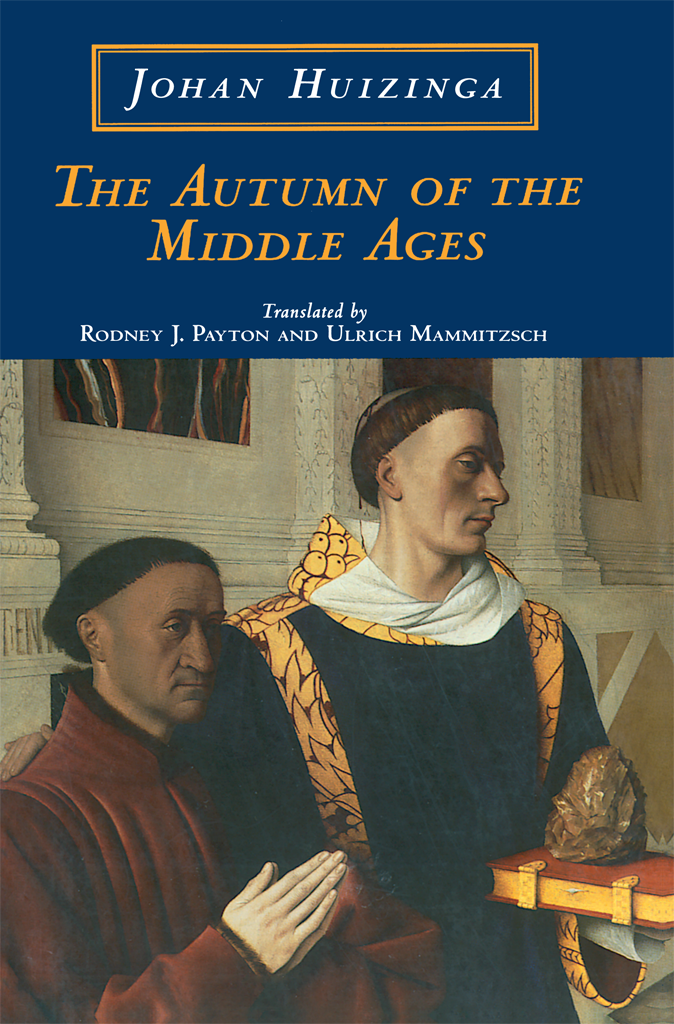
\includegraphics[width = \paperwidth, height = \paperheight] {include/html/images/1_1}}}

\begin{document}
\maketitle
\pagenumbering{gobble}

\protect\hypertarget{00_Cover.xhtml}{}{}

\protect\hypertarget{02_Copyright.xhtml}{}{}

\protect\hypertarget{02_Copyright.xhtmlux5cux23page_iv}{}{}JOHAN
HUIZINGA, born in 1872, became professor of history at the University of
Leiden in 1915 and taught there until 1942, when the Nazis closed the
university and held him hostage until shortly before his death in 1945.
His other books include \emph{Erasmus and the Age of Reformation, Homo
Ludens: A Study of the Play Element in Culture}, and \emph{Men and
Ideas: History, the Middle Ages, the Renaissance}.

RODNEY PAYTON is professor of Liberal Studies at Western Washington
University. He is the author of \emph{A Modern Reader's Guide to Dante's
Inferno}. ULRICH MAMMITZSCH (d. 1990) was professor of Liberal Studies
at Western Washington University. He is the author of \emph{Evolution of
the Garbhadhatu Mandala} and the translator of Dietrich Seckel's
\emph{The Buddhist Art of East Asia}.

The University of Chicago Press, Chicago 60637

© 1996 by The University of Chicago

All rights reserved. Published 1996

Paperback edition 1996.

Printed in the United States of America

11 10 09 08 07 06 05 04 0 3 02~~~~~~ 3 4 5 6 7

ISBN 0-226-35992-1 (cloth)

ISBN: 0-226-35994-8

ISBN 978-0-226-76768-0 (ebook)

This translation is based on the 1921 edition of \emph{Herfsttij der
Middeleeuwen}.

Library of Congress Cataloging-in-Publication Data

Huizinga, Johan, 1872--1945.

{[}Herfsttij der Middeleeuwen. English{]}

The autumn of the Middle Ages /Johan Huizinga ; translated by Rodney J.
Payton and Ulrich Mammitzsch.

p.~~~~~~~cm.

Includes bibliographical references and index.

1. France---Civilization---1328--1600. 2. Netherlands---Civilization. 3.
Civilization, Medieval. I. Title.

DC33.2.H83~~~1996

944'025---dc20

95-613

CIP


\includegraphics{include/html/images/5_1.png}
The paper used in this publication meets the minimum requirements of the
American National Standard for Information Sciences---Permanence of
Paper for Printed Library Materials, ANSI Z39.48-1992.

\tableofcontents

\frontmatter

\chapter{TRANSLATOR'S INTRODUCTION}

THE IDEA OF THIS TRANSLATION HAD ITS MOMENT of conception in Karl J.
Weintraub's class in History of Culture at the University of Chicago
(now more than twenty years ago) when Weintraub commented, with some
heat, on the deficiencies of the English translation of \emph{Herfsttij
der Middeleeuwen} that we students were using when it was compared to
the elegance of the Dutch edition he had on the lectern. The tiny
margins of my crumbling paperback are filled with all my efforts to get
down the corrections. When I began my own teaching of Huizinga's text,
which I had come to treasure, those illegible notes suggested that what
I was professing fell far short and an examination of the original
showed me that Weintraub's observations were justified. Yet, in spite of
the shortcomings of the translation, my students always responded well
to Huizinga. Later Professor Weintraub commented to me that it was an
indication of the power of its subject and style that Huizinga's book
commonly captivated readers in spite of the ``very inferior, crippled
version''\textsuperscript{\protect\hypertarget{05_TRANSLATOR_S_INTRODUCTION.xhtmlux5cux23id_2247}{\protect\hyperlink{23_NOTES.xhtmlux5cux23id_2248}{1}}}
in which it appeared in English.

Therefore when my colleague Ulrich Mammitzsch, now deceased, and I
agreed to attempt a new translation there was a certain feeling of being
the rescuers of something fine that had been corrupted and undervalued.
However, this feeling was somewhat challenged by the fact that Huizinga
not only authorized the English translation, but also apparently
collaborated with Fritz Hopman in producing it as a variant version of
the book. He specifically approved the results in the preface he wrote
for the translation.

This English edition is not a simple translation of the original Dutch
(second edition 1921, first 1919), but the result of a work of
adaptation, reduction and consolidation under the author's direction.
The references, here left out, may be found in full in the original.
.~.~.

\protect\hypertarget{05_TRANSLATOR_S_INTRODUCTION.xhtmlux5cux23page_x}{}{}The
author wishes to express his sincere thanks to .~.~. Mr. F. Hopman, of
Leiden, whose clear insight into the exigencies of translation rendered
the recasting possible, and whose endless patience with the wishes of an
exacting author made the difficult task a work of friendly
cooperation.\textsuperscript{\protect\hypertarget{05_TRANSLATOR_S_INTRODUCTION.xhtmlux5cux23id_2245}{\protect\hyperlink{23_NOTES.xhtmlux5cux23id_2246}{2}}}

Even given this endorsement by the author, I think that any studious
reader of both the Dutch (or the very accurate German translation) and
the English would conclude that the original is a much better book. The
original is nearly one-third longer and has many more citations of
original material. In the Hopman translation, blocks of text are
inexplicably moved around, and sometimes Hopman's usually good English
fails him as when he translates ``mystiek en détail'' as ``mysticism by
retail.'' It seems that Huizinga ultimately must have thought the
original better, as none of the ``adaptation, reduction and
consolidation'' found its way into subsequent Dutch printings or foreign
translations of the book with the exception of the revised arrangement
of chapters.

The route by which Huizinga arrived at the Hopman translation can be
traced in the \emph{Briefwisseling (Correspondence)}, if not, entirely,
his motivation for taking
it.\textsuperscript{\protect\hypertarget{05_TRANSLATOR_S_INTRODUCTION.xhtmlux5cux23id_2243}{\protect\hyperlink{23_NOTES.xhtmlux5cux23id_2244}{3}}}
Huizinga had begun negotiations with the French publisher Edouard
Champion of Paris, who preferred a shortened version of the book and
without the references. This project fell through, owing to
disagreements over the rights of publication of the French edition in
Holland in 1923 (letter 457), and Huizinga was left with the condensed,
but unpublished, French manuscript. (An accurate French edition was
eventually published by the firm of Payot in 1932, in a translation by
Julia Bastin {[}letter 559{]}.) In 1923, Huizinga was also negotiating
with Edward Arnold and Company about an English edition, and, owing to
the fact that Arnold had no one in their office who could read Dutch,
they reviewed it in the condensed French version. Sir Rennell Rodd, a
diplomat, poet, and historian, and Arnold's reviewer, thought the
original form of the book would sell only to scholars and preferred it
in its French form, which he thought might have a popular audience
(letter 462) and, although Huizinga protested, he did not do so very
strongly (letter 466). An abridgment on the lines of the French
manuscript was ultimately ageed upon (letters 472 and 477) and the
Hopman version, called \emph{The Waning of the Middle Ages}, is the
result.

\protect\hypertarget{05_TRANSLATOR_S_INTRODUCTION.xhtmlux5cux23page_xi}{}{}All
this was taking place while the final arrangements for the German
edition were being set. The German edition is precise in all
particulars, but the fourteen original Dutch chapters are broken up into
twenty-three, which are more even in length. This was Huizinga's own
idea, evidently incorporated in the unpublished French translation and
eventually carried forward in the English as well (letter 470).

Thus Huizinga clearly preferred a complete translation of
\emph{Herfsttij}, although he did think the chapter divisions could be
improved. His quarrel with Champion over distribution rights, however,
suggests that remuneration was an important issue, as he raised
practically no objections to the condensation ultimately produced by
Hopman for Arnold and Company. It is possible, too, given that the
prospect of a wide market for the book might have had something to do
with his thinking, that in obtaining an English edition Huizinga was
also looking forward to the American market. Huizinga wrote two books
about America, both gently
critical.\textsuperscript{\protect\hypertarget{05_TRANSLATOR_S_INTRODUCTION.xhtmlux5cux23id_2241}{\protect\hyperlink{23_NOTES.xhtmlux5cux23id_2242}{4}}}
Like his contemporary Freud, Huizinga thought American life suffered
from its lack of social forms; he considered Americans to be
materialistic and far, far too hasty in the pursuit of their affairs. He
invented a motto for America, ``This Here, and Soon,'' to characterize
this haste, which, he thought, all too often, led to superficiality.
Perhaps this perception caused him to believe that a simplified and less
allusive \emph{Autumn} might succeed best in the American market. The
fourteen uneven Dutch chapters became the twenty-three short chapters as
in the German edition, much more suitable for daily classroom
assignments and for a people with a short attention span. The work of
preparing the English translation was given to Fritz Hopman, a student
of English literature and journalist, who at one time was chairman of
the Maatschappij der Nederlandse Letterkunde (Dutch Literature Society).
He was in financial difficulties in 1924, and Huizinga was probably glad
to be able to provide him with
work.\textsuperscript{\protect\hypertarget{05_TRANSLATOR_S_INTRODUCTION.xhtmlux5cux23id_2239}{\protect\hyperlink{23_NOTES.xhtmlux5cux23id_2240}{5}}}

F. W. N. Hugenholtz's study of the history of the text, \emph{The Fame
of a
Masterwork},\textsuperscript{\protect\hypertarget{05_TRANSLATOR_S_INTRODUCTION.xhtmlux5cux23id_2237}{\protect\hyperlink{23_NOTES.xhtmlux5cux23id_2238}{6}}}
shows that the first recognition of the book's importance came, not from
Huizinga's Dutch colleagues, but in German reviews. The Dutch were
inclined to consider \emph{The Autumn of the Middle
Ages\textsuperscript{\protect\hypertarget{05_TRANSLATOR_S_INTRODUCTION.xhtmlux5cux23id_2235}{\protect\hyperlink{23_NOTES.xhtmlux5cux23id_2236}{7}}}}
far too literary for serious history and mistakenly thought its approach
to be old-fashioned rather than realizing that it was truly a
revolutionary innovation. \emph{Autumn} was Huizinga's first major work
published after he became professor of history at
\protect\hypertarget{05_TRANSLATOR_S_INTRODUCTION.xhtmlux5cux23page_xii}{}{}Leiden,
and Leiden was not at that time Holland's ``first'' university, nor was
Huizinga the most famous professor of history. Defensive, in the face of
native criticism of the work he might, indeed, have considered the
English translation a step to a further revision (the second Dutch
edition had appeared in 1921, the Hopman translation came out in 1924).
It seems to me, that much of what is left out of the Hopman version are
elements which contribute to the ``literary,'' that is to say aesthetic
character of the book and this might be a direct response to his Dutch
critics.

There is another possible reason for the truncated English version.
Probably anyone who reads \emph{Autumn} will notice that it reveals a
great deal of the private side of Huizinga himself. In it, the reader
sees not only Huizinga's opinions and strong convictions, but glimpses
his passions and, I think, his spiritual side as well. Perhaps he
realized this and the drawing back so apparent in the original English
is an instinctive reaction that he also exhibited in other
circumstances.

In his brief autobiography written at the very end of his
life\textsuperscript{\protect\hypertarget{05_TRANSLATOR_S_INTRODUCTION.xhtmlux5cux23id_2233}{\protect\hyperlink{23_NOTES.xhtmlux5cux23id_2234}{8}}}
Huizinga reveals that he consistently hid his true self even from his
colleagues and students. ``It is not false modesty when I say that,
though I have been known as an early riser since childhood, I never rose
quite as early as people believed.'' The relationship of his work to his
private self was frequently misjudged by others. Huizinga almost seems
pleased at their confusion.

Regarding my biography of Erasmus, many people have expressed the view
that here was a man after my own heart. As far as I can tell, nothing
could be farther from the truth for, much though I admire Erasmus, he
inspires me with little sympathy and, as soon as the work was done, I
did my best to put him out of my mind. I remember a conversation in
January 1932 with a German colleague who contended that \emph{Erasmus}
was much more my line of country than the \emph{Waning of the Middle
Ages} with which, he claimed, I must have struggled manfully. I thought
about the matter for a moment and then I had to smile. In fact, my
historical and literary studies never struck me as partaking of the
nature of struggle in any way, nor any of my work as a great challenge.
Indeed, the whole idea of having to overcome enormous obstacles was as
alien to me as having to compete in a
\protect\hypertarget{05_TRANSLATOR_S_INTRODUCTION.xhtmlux5cux23page_xiii}{}{}race,
as alien as the spirit of competition whose importance in cultural life
I myself have emphasized in my \emph{Homo Ludens}.

When he finds himself on the edge of a deep personal revelation,
Huizinga goes so far, and no further.

.~.~. In September 1899, I was granted two weeks' extra leave,
immediately after beginning of term, to attend the Congress of
Orientalists in Rome. I went there with J. P. Vogel, who intended to go
on to India, and with André Jolles with whom I had started a close
friendship in the autumn of 1896. This friendship was to play a large
part in my life for more than 35 years, until 9th October 1933 when it
was abruptly cut short---and not by me. I could write a whole book on my
relation with Jolles, so full is my mind of him and despite all that has
happened---my heart as well.

Huizinga's later works do not reveal the personality of the author as
much as \emph{Autumn} does. A prominent sense of the author only again
becomes apparent in his great moral essay of the thirties, \emph{In the
Shadow of
Tomorrow.\textsuperscript{\protect\hypertarget{05_TRANSLATOR_S_INTRODUCTION.xhtmlux5cux23id_2231}{\protect\hyperlink{23_NOTES.xhtmlux5cux23id_2232}{9}}}}

Given Huizinga's importance to historiography, the fact that the English
translation is a variant text has not been given enough attention. With
the single exception of Weintraub, no one, to my knowledge, has pointed
out the critical importance of that fact, even though the introduction
might have served as a warning to a professionally critical discipline.
Is it possible that English-speaking historians have been discussing
this book with their foreign colleagues without realizing that they were
reading a significantly different text? If this is so, it is a primary
justification for the present translation.

Hopman's work does have the virtue of being graceful. He did have an
excellent grasp of English vocabulary, and his rendition is sometimes
lovely, but it is not literal and sometimes something more than a
literal quality is missing. It is not proper for a translator in the
second place to judge too harshly the work of a predecessor, but a
reader deserves some indication why one translation should be preferred
over another. The most glaring changes in the Hopman from the Dutch
second edition are the many omissions of
\protect\hypertarget{05_TRANSLATOR_S_INTRODUCTION.xhtmlux5cux23page_xiv}{}{}examples
drawn from the (in most instances) medieval French sources that Huizinga
cites in the original language (although there are a few instances where
Hopman includes examples not in the Dutch edition). The present
translators felt that the original divisions of the text much more
clearly reflected the organization of Huizinga's argument in spite of
their rather uneven lengths and Huizinga's second thoughts about the
matter. Finally, the Hopman translation omits, as its introduction
points out, the documentation. These alterations are restored in this
translation.

Much more serious issues are those alterations by Hopman that tend to
distort Huizinga's meaning. Hopman is sometimes prone to pull Huizinga's
punches. For instance, one of the most significant elements in
\emph{Autumn} is its assertions about the proper use of sources, an
issue addressed several times. Here is a representative passage in this
translation:

Daily life offered unlimited range for acts of flaming passion and
childish imagination. Our medieval historians who prefer to rely as much
as possible on official documents because the chronicles are unreliable
fall thereby victim to an occasionally dangerous error. The documents
tell us little about the difference in tone that separates us from those
times; they let us forget the fervent pathos of medieval life. Of all
the passions permeating medieval life with their color, only two are
mentioned, as a rule by legal documents: greed and quarrelsomeness. Who
has not frequently wondered about the nearly incredible violence and
stubbornness with which greed, pugnacity, or vindictiveness rise to
prominence in the court documents of that period! It is only in the
general context of the passions which inflame every sphere of life that
these tensions become acceptable and intelligible to us. This is why the
authors of the chronicles, no matter how superficial they may be with
respect to the actual facts and no matter how often they may err in
reporting them, are indispensable if we want to understand that age
correctly.

And here is the same passage in Hopman:

A scientific historian of the Middle Ages, relying first and foremost on
official documents, which rarely refer to the
\protect\hypertarget{05_TRANSLATOR_S_INTRODUCTION.xhtmlux5cux23page_xv}{}{}passions,
except violence and cupidity, occasionally runs the risk of neglecting
the difference of tone between the life of the expiring Middle Ages and
that of our own days. Such documents would sometimes make us forget the
vehement pathos of medieval life, of which the chroniclers, however
defective as to material facts, always keep us in mind.

Not only has Hopman made a strong statement weak, his version misses the
nuance of just how passionate Huizinga was about the passions of the
Middle Ages.

Similar distortions frequently occur. Here is Hopman's translation of a
passage about the profane interest in such things as Mary's marital
relationship with Joseph:

This familiarity with sacred things is, on the one hand, a sign of deep
and ingenuous faith; on the other, it entails irreverence whenever
mental contact with the infinite fails. Curiosity, ingenuous though it
be, leads to profanation.

Here is this translation:

This fatuous familiarity with God in daily life has to be seen in two
ways. On the one hand it testifies to the absolute stability and
immediacy of faith, but where this familiarity becomes habitual, it
increases the danger that the godless (who are always with us), but also
the pious, in moments of insufficient religious tension, continuously
profane faith more or less consciously and intentionally.

For the student interested in historiography itself, perhaps the
omissions of theoretical statements are the most serious. In the famous
discussion of the three routes to the beautiful life in the second
chapter, Hopman omits this statement of serious interest to anyone
concerned with Huizinga's definitions of culture and civilization and
with the movement of his thinking towards the theoretical statement of
\emph{Homo
Ludens},\textsuperscript{\protect\hypertarget{05_TRANSLATOR_S_INTRODUCTION.xhtmlux5cux23id_2229}{\protect\hyperlink{23_NOTES.xhtmlux5cux23id_2230}{10}}}
which defines the role of play in culture.

The great divide in the perception of the beauty of life comes much more
between the Renaissance and the Modern Period than between the Middle
Ages and the Renaissance. The turnabout occurs at the point where art
and life begin to diverge. It is the point where art begins to be no
longer
\protect\hypertarget{05_TRANSLATOR_S_INTRODUCTION.xhtmlux5cux23page_xvi}{}{}in
the midst of life, as a noble part of the joy of life itself, but
outside of life as something to be highly venerated, as something to
turn to in moments of edification or rest. The old dualism separating
God and world has thus returned in another form, that of the separation
of art and life. Now a line has been drawn right through the enjoyments
offered by life. Henceforth they are separated into two halves---one
lower, one higher. For medieval man they were all sinful without
exception; now they are all considered permissible, but their ethical
evaluation differs according to their greater or lesser degree of
spirituality.

The things which can make life enjoyable remain the same. They are, now
as before, reading, music, fine arts, travel, the enjoyment of nature,
sports, fashion, social vanity (knightly orders, honorary offices,
gatherings) and the intoxication of the senses. For the majority, the
border between the higher and lower levels seems now to be located
between the enjoyment of nature and sports. But this border is not firm.
Most likely sport will sooner or later again be counted among the higher
enjoyments---at least insofar as it is the art of physical strength and
courage. For medieval man the border lay, in the best of cases, right
after reading; the enjoyment of reading could only be sanctified through
striving for virtue or wisdom. For music and the fine arts, it was their
service to faith alone which was recognized as being good. Enjoyment
\emph{per se} was sinful. The Renaissance had managed to free itself
from the rejection of all the joy of life as something sinful, but had
not yet found a new way of separating the higher and lower enjoyments of
life; the Renaissance wanted an unencumbered enjoyment of all of life.
The new distinction is the result of the compromise between the
Renaissance and Puritanism that is at the base of modern spiritual
attitudes. It amounted to a mutual capitulation in which the one side
insisted on saving beauty while the other insisted on the condemnation
of sin. Strict Puritanism, just as did the Middle Ages, still condemned
as basically sinful and worldly the entire sphere of the beautification
of life with an exception being made in cases where such efforts assumed
expressly religious forms and sanctified themselves through their use in
the service of faith. Only
\protect\hypertarget{05_TRANSLATOR_S_INTRODUCTION.xhtmlux5cux23page_xvii}{}{}after
the Puritan worldview lost its intensity did the Renaissance
receptiveness to all the joys of life gain ground again; perhaps even
more ground than before because, beginning with the eighteenth century
there is a tendency to regard the natural \emph{per se} an element of
the ethically good. Anyone attempting to draw the dividing line between
the higher and lower enjoyment of life according to the dictates of
ethical consciousness would no longer separate art from sensuous
enjoyment, the enjoyment of nature from the cult of the body, the
elevated from the natural, but would only separate egotism, lies, and
vanity from purity.

There are many such issues to which we could point, not in the spirit of
demeaning a translation that has served Huizinga well, but in the sense
that having done its work and brought the importance of the mind of
Huizinga to the attention of the English-speaking world, it is now
obsolete and a more critical and deeper look at Huizinga requires access
to a version of the work closer to that known by the rest of the world.

This translation was made from the second Dutch edition of 1921. Seen
from the vantage point of the second edition, the first has a tentative
character that Huizinga eliminated in his revision. Huizinga made
further minor revisions in later editions, but the second represents his
thinking at its most seminal stage. We compared our work carefully with
the German translation of 1924, which, Huizinga notes, follows the
second Dutch edition exactly. We have included not only the preface to
the Dutch edition, but also the preface that Huizinga wrote for the
German translation, for the insight it gives into the title and its
comment on the question of translation itself. We have restored the
documentation and added a few translators' notes to clarify Huizinga's
references to things that might be common knowledge or self-evident to a
Dutch reader but not necessarily so to others. This version also
includes translations of the citations that Huizinga makes in the
original languages. Such translations have become customary in later
editions, although they do not appear in the Dutch original we followed.
Our translations follow Hopman, but we have made several alterations
according to our own judgment.

*~~~*~~~*

\protect\hypertarget{05_TRANSLATOR_S_INTRODUCTION.xhtmlux5cux23page_xviii}{}{}Ulrich
Mammitzsch, my colleague and co-translator, was a noted specialist in
Buddhist art and literature, but his formidable erudition extended to
great works of all cultures and he was as pleased to discuss Schiller as
he was his beloved mandalas. He felt a special affinity for Huizinga,
who began his academic life as a student of Eastern culture, and who had
a love of literature much like Ulrich's. Mostly, however, Ulrich's
dedication to Huizinga was because they were alike in their
high-mindedness. As Ulrich Mammitzsch fled the East Zone, not because of
political theory, but because he found the Communists to be unethical,
so Johan Huizinga was brought to denounce the Nazis from the first
principles of civilized behavior. The two minds spoke to one another
directly and I will never forget Ulrich's excitement as we read
Huizinga's description of the tension in the life of medieval common
people, strung between the church and the nobility---a tension which,
Ulrich exclaimed, he had seen the last of as a child in rural Germany
before the war. He read the book from the inside, so to speak, and I
would like to attribute whatever virtues this translation has to his
insightful sensitivity.

\emph{RODNEY J. PAYTON}

\chapter{PREFACE TO THE FIRST AND SECOND DUTCH EDITIONS}

IN MOST INSTANCES IT IS THE ORIGIN OF THE NEW that attracts the
attention of the mind to the past. We want to know how the new ideas and
the forms of life that shine in their fullness during later times came
to be. We view past ages primarily in terms of the promise they hold for
those that follow. How eagerly the Middle Ages have been scrutinized for
evidence of the first sprouts of modern culture, so eagerly that it
sometimes must appear as if the intellectual history of the Middle Ages
was nothing but the advent of the Renaissance. Did we not see everywhere
in this age, which was once regarded as rigid and dead, new growths that
all seemed to point to future perfection? Yet in our search for newly
arising life it is easily forgotten that in history, as in nature, the
processes of death and birth are eternally in step with one another. Old
forms of thought die out while, at the same time and on the same soil, a
new crop begins to bloom.

This book is an attempt to view the time around the fourteenth and
fifteenth centuries, not as announcing the Renaissance, but as the end
of the Middle Ages, as the age of medieval thought in its last phase of
life, as a tree with overripe fruits, fully unfolded and developed. The
luxuriant growth of old compelling forms over the living core of
thought, the drying and rigidifying of a previously valid store of
thought: this is the main content of the following pages. In writing
this text, my eye was trained on the depth of the evening sky, a sky
steeped blood red, desolate with threatening leaden clouds, full of the
false glow of copper. Looking back at what I have written, the question
arises whether, if my eye had dwelt still longer on the evening sky, the
turbid colors may yet have dissolved into utter clarity. It also seems
quite possible that the image, now that I have given it contours and
colors, may yet have become more gloomy and less serene than I had
perceived it
\protect\hypertarget{06_PREFACE_TO_THE_DUTCH_EDITION.xhtmlux5cux23page_xx}{}{}when
I started my labors. It can easily happen to one who has his vision
trained downward that what he perceives becomes too decrepit and wilted,
that too much of the shadow of death has been allowed to fall upon his
work.

The point of departure for this work was the attempt to better
understand the work of the van Eycks and that of their successors and to
understand it within the context of the entire life of that age. The
Burgundian community was the frame of reference that I had in mind: it
seemed possible to view this community as a civilization in its own
right, just like the Italian community of the fourteenth century; the
title of the work was first set as \emph{The Century of Burgundy}. But
as the scope of this civilization was viewed in a wider perspective,
certain limitations had to be abandoned. Just to retain the notion of a
postulated unity of Burgundian culture meant that non-Burgundian France
had to be given at least as much attention. Thus the place of Burgundy
was taken by the dual entities of France and the Netherlands and that in
a very different way. While in viewing the dying medieval culture the
Dutch element lags behind the French, there are areas where that element
has its own significance: in the life of piety and that of art. These
are given the opportunity to speak in greater detail.

There is no need to defend the crossing of the fixed geographic
boundaries in the tenth chapter so as to call on, next to Ruusbroec and
Denis the Carthusian, on Eckhardt, Suso, and Tauler as witnesses. How
little my story is justified by the writings I have studied from the
fourteenth and fifteenth centuries compared to all those I wanted to
read. How much I would have liked to place, next to the evolution of the
main types of the different intellectual traditions on which some of the
notions of these figures are often based, yet still others. But if I
relied among the historiographers on Froissart and Chastellain more than
on others, among the poets on Eustache Deschamps, among the theologians
on Jean de Gerson and Denis the Carthusian, among the painters on Jan
van Eyck---so is this not only the result of the limitation of my
material, but even more so the result of the richness of their works and
the singularly keen way in which their expressions are the preeminent
mirror of the spirit of their age.

It is the forms of life and thought that are used as evidence here. To
capture the essential content that rests in the form: is this not the
proper task of historical study?

\chapter{PREFACE TO THE GERMAN TRANSLATION}

THE NEED TO BETTER UNDERSTAND THE ART OF THE van Eyck brothers and that
of their successors and to view these artists in the context of the life
of their time provided the first impetus for this book. But a different,
in many respects more comprehensive image emerged during the course of
the investigation. It became evident that the fourteenth and fifteenth
centuries in France and in the Netherlands in particular are much more
suited to give us a sense of the end of the Middle Ages and of the last
manifestation of medieval culture than they are to demonstrate to us the
awakening Renaissance.

Our minds prefer to concern themselves with ``origins'' and
``beginnings.'' In most instances the promise that ties one age to its
successor appears to be more important than the memories that link it to
its predecessor. As a result, the search to find the first sprouts of
modern culture in medieval culture was carried out so eagerly and to the
point that the term medieval period itself came to be questioned and it
appeared as if this epoch was barely something other than the age that
ushered in the Renaissance. But dying and becoming keep just as much
pace with each other in history as in nature. To trace the vanishing of
overripe cultural forms is not less significant---and by no means less
fascinating---than to trace the arising of new forms. We do more
justice, not only to artists like the van Eycks, but also to {[}poets
such as{]} Eustache Deschamps, historiographers such as Froissart and
Chastellain, theologians such as Jean de Gerson and Denis the
Carthusian, and to all representatives of the spirit of this age if we
view them not as initiating and heralding what is to come, but rather as
completing the forms of an age in its final stage.

The author was, at the time he wrote this book, less aware than now of
the danger of comparing historical periods to the seasons of the year;
he asks therefore that the title of the book be taken
\protect\hypertarget{07_PREFACE_TO_THE_GERMAN_TRANSLATIO.xhtmlux5cux23page_xxii}{}{}only
as a figure of speech that is intended to capture the general mood of
the whole.

The translation follows exactly the second revised Dutch edition of 1921
(the first appeared in 1919). If the German tongue still tastes in
places the flavor of the Dutch original, we should remind ourselves that
a translation in the strict sense of the word is an impossibility even
in so closely related languages such as German and Dutch. Why should we
be so eager to obliterate fearfully the traces of what is foreign in
that which is of foreign origin?

Many have supported this work of translation in a valuable way. We owe a
debt of gratitude, next to the translator, primarily to our friends
Prof. André Jolles (Leipzig), Prof. W. Vogelsang (Utrecht), and Paul
Lehman (Munich). My sincere expression of thanks for his valuable
contribution to this work go to Prof. Eugene Lerch, who took it upon
himself to translate the French quotations found in the appended
section.

Leiden

November 1923

\mainmatter

\chapter{THE PASSIONATE INTENSITY OF LIFE}

WHEN THE WORLD WAS HALF A THOUSAND YEARS younger all events had much
sharper outlines than now. The distance between sadness and joy, between
good and bad fortune, seemed to be much greater than for us; every
experience had that degree of directness and absoluteness that joy and
sadness still have in the mind of a child. Every event, every deed was
defined in given and expressive forms and was in accord with the
solemnity of a tight, invariable life style. The great events of human
life---birth, marriage, death---by virtue of the sacraments, basked in
the radiance of the divine mystery. But even the lesser events---a
journey, labor, a visit---were accompanied by a multitude of blessings,
ceremonies, sayings, and conventions.

There was less relief available for misfortune and for sickness; they
came in a more fearful and more painful way. Sickness contrasted more
strongly with health. The cutting cold and the dreaded darkness of
winter were more concrete evils. Honor and wealth were enjoyed more
fervently and greedily because they contrasted still more than now with
lamentable poverty. A fur-lined robe of office, a bright fire in the
oven, drink and jest, and a soft bed still possessed that high value for
enjoyment that perhaps the English novel, in describing the joy of life,
has affirmed over the longest period of time. In short, all things in
life had about them something glitteringly and cruelly public. The
lepers, shaking their rattles and holding processions, put their
deformities openly on display. Every estate, order, and craft could be
recognized by its dress. The notables, never appearing without the
ostentatious display of their weapons and liveried servants, inspired
awe and envy. The administration of justice, the sales of goods,
weddings and funerals---all announced themselves through processions,
shouts, lamentations and music. The lover carried the emblem of his
lady, the member
\protect\hypertarget{08_Chapter_One__THE_PASSIONATE_INTE.xhtmlux5cux23page_2}{}{}the
insignia of his fraternity, the party the colors and coat of arms of its
lord.

In their external appearance, too, town and countryside displayed the
same contrast and color. The city did not dissipate, as do our cities,
into carelessly fashioned, ugly factories and monotonous country homes,
but, enclosed by its walls, presented a completely rounded picture that
included its innumerable protruding towers. No matter how high and
weighty the stone houses of the noblemen or merchants may have been,
churches with their proudly rising masses of stone, dominated the city
silhouettes.

Just as the contrast between summer and winter was stronger then than in
our present lives, so was the difference between light and dark, quiet
and noise. The modern city hardly knows pure darkness or true silence
anymore, nor does it know the effect of a single small light or that of
a lonely distant shout.

From the continuing contrast, from the colorful forms with which every
phenomenon forced itself on the mind, daily life received the kind of
impulses and passionate suggestions that is revealed in the vacillating
moods of unrefined exuberance, sudden cruelty, and tender emotions
between which the life of the medieval city was suspended.

But one sound always rose above the clamor of busy life and, no matter
how much of a tintinnabulation, was never confused with other noises,
and, for a moment, lifted everything into an ordered sphere: that of the
bells. The bells acted in daily life like concerned good spirits who,
with their familiar voices, proclaimed sadness or joy, calm or unrest,
assembly or exhortation. People knew them by familiar names: Fat
Jacqueline, Bell Roelant; everyone knew their individual tones and
instantly recognized their meaning. People never became indifferent to
these sounds, no matter how overused they were. During the notorious
duel between two burghers of Valenciennes in 1455 that kept the city and
the entire court of Burgundy in extraordinary suspense, the great bell
sounded as long as the fight lasted, ``laquelle fait hideux a
oyr''\protect\hypertarget{08_Chapter_One__THE_PASSIONATE_INTE.xhtmlux5cux23id_2303}{\protect\hyperlink{23_NOTES.xhtmlux5cux23id_2304}{*\textsuperscript{11}}}
says
Chastellain,\textsuperscript{\protect\hypertarget{08_Chapter_One__THE_PASSIONATE_INTE.xhtmlux5cux23id_2226}{\protect\hyperlink{23_NOTES.xhtmlux5cux23page_398}{2}}}
``Sonner l'effroy,'' ``faire l'effroy ``was what the ringing of the
alarm bell was
called.\textsuperscript{\protect\hypertarget{08_Chapter_One__THE_PASSIONATE_INTE.xhtmlux5cux23id_2224}{\protect\hyperlink{23_NOTES.xhtmlux5cux23id_2225}{3}}}
How deafening the sound must have been when the bells of all the
churches and cloisters of Paris pealed all day, or even all night,
because a pope had been
\protect\hypertarget{08_Chapter_One__THE_PASSIONATE_INTE.xhtmlux5cux23page_3}{}{}elected
who was to end the schism or because peace had been arranged between
Burgundy and
Armagnac.\textsuperscript{\protect\hypertarget{08_Chapter_One__THE_PASSIONATE_INTE.xhtmlux5cux23id_2222}{\protect\hyperlink{23_NOTES.xhtmlux5cux23id_2223}{4}}}

Processions must have also been deeply moving. During sad times---and
these came often---they could occasionally take place day after day even
for weeks on end. In 1412, when the fatal conflict between the houses of
Orléans and Burgundy had finally led to open civil war, King Charles VI
seized the oriflamme so that he and John the Fearless could fight
against the Armagnacs, who, by virtue of their alliance with England,
had become traitors to their country. Daily processions were ordered to
be held in Paris as long as the king was on foreign soil. They continued
from the end of May into July and involved ever different groups, orders
or guilds, ever different routes and ever different relics: ``les plus
piteuses processions qui oncques eussent été veues de aage de
homme.''\protect\hypertarget{08_Chapter_One__THE_PASSIONATE_INTE.xhtmlux5cux23id_2252}{\protect\hyperlink{23_NOTES.xhtmlux5cux23id_2251}{*\textsuperscript{2}}}
All were barefoot with empty stomachs, members of parliament and poor
burghers alike; every one who was able carried a candle or a torch.
There were always many small children with them. Even the poor country
folk from the villages around Paris came running on bare feet.
Processions were joined or watched, ``en grant pleur, en grant lermes,
en grant
devocion.''\protect\hypertarget{08_Chapter_One__THE_PASSIONATE_INTE.xhtmlux5cux23id_2250}{\protect\hyperlink{23_NOTES.xhtmlux5cux23id_2249}{†\textsuperscript{3}}}
And heavy rain fell almost constantly during the entire
period.\textsuperscript{\protect\hypertarget{08_Chapter_One__THE_PASSIONATE_INTE.xhtmlux5cux23id_2220}{\protect\hyperlink{23_NOTES.xhtmlux5cux23id_2221}{5}}}

Then there were the princely entry processions prepared with all the
varied formal skills at the disposal of the main actors. And, with
uninterrupted frequency, there were executions. The gruesome fascination
and coarse compassion stirred at the place of execution became an
important element in the spiritual nourishment of the people. For
dealing with vicious robbers and murderers the courts invented terrible
punishments: in Brussels a young arsonist and murderer was tied with a
chain so that he could move in a circle about a stake surrounded by
burning bundles of fagots. He introduced himself to the people in moving
words as a warning example: ``et tellement fit attendrir les coeurs que
tout le monde fondoit en larmes de compassion.'' ``Et fut sa fin
reccommandée la plus belle que l'on avait oncques
vue.''\textsuperscript{\protect\hypertarget{08_Chapter_One__THE_PASSIONATE_INTE.xhtmlux5cux23id_2218}{\protect\hyperlink{23_NOTES.xhtmlux5cux23id_2219}{6}}}\protect\hypertarget{08_Chapter_One__THE_PASSIONATE_INTE.xhtmlux5cux23id_2256}{\protect\hyperlink{23_NOTES.xhtmlux5cux23id_2255}{‡\textsuperscript{4}}}
During the Burgundian reign of terror in Paris, Messire Nansart du Bois,
an Armagnac,
\protect\hypertarget{08_Chapter_One__THE_PASSIONATE_INTE.xhtmlux5cux23page_4}{}{}was
beheaded. Not only did he grant forgiveness to the executioner, who, as
was customary, requested it, but he even asked to be kissed by him.
``Foison de peuple y avoit, qui quasi tous ploroient à chaudes
larmes.''\textsuperscript{\protect\hypertarget{08_Chapter_One__THE_PASSIONATE_INTE.xhtmlux5cux23id_2216}{\protect\hyperlink{23_NOTES.xhtmlux5cux23id_2217}{7}}}\protect\hypertarget{08_Chapter_One__THE_PASSIONATE_INTE.xhtmlux5cux23id_2254}{\protect\hyperlink{23_NOTES.xhtmlux5cux23id_2253}{*\textsuperscript{5}}}
Frequently the sacrificial victims were great lords; in those cases the
people had the even greater satisfaction of witnessing stern justice and
a more forceful warning about the insecurity of high position than would
be conveyed by a painting or a \emph{danse
macabre}.\textsuperscript{\protect\hypertarget{08_Chapter_One__THE_PASSIONATE_INTE.xhtmlux5cux23id_2214}{\protect\hyperlink{23_NOTES.xhtmlux5cux23id_2215}{8}}}
The authorities took pains that nothing was lacking in the impression
the spectacle made. The nobles took their last walk bedecked in the
symbols of their greatness. Jean de Montaigu, grand maitre d'hotel of
the king and a victim of the hatred of John the Fearless, travels to the
gallows seated high on top of a cart. Two trumpeters precede him. He is
dressed in his robes of state, cap, vest, and pants---half white, half
red---with golden spurs on his feet. The beheaded body was left hanging
on the gallows still wearing those golden spurs. The wealthy canon
Nicholas d'Orgemont---who fell victim to the vendetta of the Armagnacs
in 1416---was carried through Paris on a garbage cart, clad in a wide
purple cloak and cap of the same color to witness the execution of two
of his comrades before he was led away to lifelong captivity: ``au pain
de doleur et à eaue
d'angoisse.''\protect\hypertarget{08_Chapter_One__THE_PASSIONATE_INTE.xhtmlux5cux23id_2257}{\protect\hyperlink{23_NOTES.xhtmlux5cux23id_2258}{†\textsuperscript{6}}}
The head of Maître Oudart de Bussy, who had turned down a place in
parliament, was exhumed by special order of Louis XI and, dressed with a
crimson, fur-lined hood, ``selon la mode des conseillers de
parlement,''\protect\hypertarget{08_Chapter_One__THE_PASSIONATE_INTE.xhtmlux5cux23id_2259}{\protect\hyperlink{23_NOTES.xhtmlux5cux23id_2261}{‡\textsuperscript{7}}}
was put on display with an attached explanatory poem in the town square
of Hesdin. The king himself writes about this case with grim
humor.\textsuperscript{\protect\hypertarget{08_Chapter_One__THE_PASSIONATE_INTE.xhtmlux5cux23id_2212}{\protect\hyperlink{23_NOTES.xhtmlux5cux23id_2213}{9}}}

Rarer than the processions and executions were the sermons given by
itinerant preachers who came, from time to time, to stir the people with
their words. We, readers of newspapers, can hardly imagine anymore the
tremendous impact of the spoken word on naive and ignorant minds. The
popular preacher Brother Richard, who may have served Jeanne d'Arc as
father confessor, preached in Paris in 1429 for ten days running. He
spoke from five until ten
\protect\hypertarget{08_Chapter_One__THE_PASSIONATE_INTE.xhtmlux5cux23page_5}{}{}or
eleven o'clock in the morning in the Cemetery of the Innocents---where
the famous \emph{danse macabre} had been painted---with his back to the
bone chambers where skulls were piled up above the vaulted walkways to
be viewed by the visitors. When he informed his audience after his tenth
sermon that it would have to be his last since he had not received
permission for any more, ``les gens grans et petiz plouroient si
piteusement et si fondement, comme s'ilz veissent porter en terre leurs
meilleurs amis, et lui
aussi.''\protect\hypertarget{08_Chapter_One__THE_PASSIONATE_INTE.xhtmlux5cux23id_2260}{\protect\hyperlink{23_NOTES.xhtmlux5cux23id_2263}{*\textsuperscript{8}}}
When he finally leaves Paris, the people believe that the next Sunday he
will still preach at St. Denis; a large number, perhaps as many as six
thousand, according to the Burgher of Paris, leave the city on Saturday
evening and spend the night out in the fields in order to secure good
places.\textsuperscript{\protect\hypertarget{08_Chapter_One__THE_PASSIONATE_INTE.xhtmlux5cux23id_2210}{\protect\hyperlink{23_NOTES.xhtmlux5cux23id_2211}{10}}}

Antoine Fradin, a Franciscan, was also prohibited from preaching in
Paris, because he railed against evil government. But this is precisely
what made him so beloved by the people. They guarded him day and night
in the monastery of the Cordeliers; the women stood watch with their
ammunition of ashes and stones ready. People laughed at the proclamation
prohibiting the watch: the king knows nothing about it! When Fradin is
finally banned and has to leave the city, the people give him an escort,
``crians et soupirans moult fort son
departement.''\textsuperscript{\protect\hypertarget{08_Chapter_One__THE_PASSIONATE_INTE.xhtmlux5cux23id_2208}{\protect\hyperlink{23_NOTES.xhtmlux5cux23id_2209}{11}}}\protect\hypertarget{08_Chapter_One__THE_PASSIONATE_INTE.xhtmlux5cux23id_2262}{\protect\hyperlink{23_NOTES.xhtmlux5cux23id_2264}{†\textsuperscript{9}}}

In all cities where the saintly Dominican Vincent Ferrer comes to
preach, the people, the magistrates, the clergy---including bishops and
prelates---go out to welcome him, singing his praises. He travels with a
large numbers of supporters, who, every evening after sunset, go on
processions with flagellations and songs. In every town he is joined by
new followers. He has carefully arranged for the food and lodging of all
his companions by employing men of spotless reputation as his
quartermasters. Numerous priests from different orders travel with him
so that they can assist him in taking confessions and celebrating mass.
A few notaries accompany him to record the legal reconciliations that
the holy preacher manages to arrange wherever he goes. When he preaches,
a wooden frame has to protect him and his entourage against the
\protect\hypertarget{08_Chapter_One__THE_PASSIONATE_INTE.xhtmlux5cux23page_6}{}{}throngs
who want to kiss his hand or his gown. Work comes to a standstill as
long as he speaks. It was a rare occasion when he failed to move his
audience to tears, and when he spoke of Judgment Day and the pains of
hell or of the sufferings of the Lord, he, just as his audience, broke
into such great tears that he had to remain silent, for a time, until
the weeping had stopped. The penitents fell to their knees before all
the onlookers to tearfully confess their great
sins.\textsuperscript{\protect\hypertarget{08_Chapter_One__THE_PASSIONATE_INTE.xhtmlux5cux23id_2206}{\protect\hyperlink{23_NOTES.xhtmlux5cux23id_2207}{12}}}
When the famous Olivier Maillard gave the Lenten sermon at Orléans in
1485, so many people climbed on the roofs of the houses that the roofers
submitted claims for sixty-four days of repair
work.\textsuperscript{\protect\hypertarget{08_Chapter_One__THE_PASSIONATE_INTE.xhtmlux5cux23id_2204}{\protect\hyperlink{23_NOTES.xhtmlux5cux23id_2205}{13}}}

All this has the atmosphere of the English-American revivals or of the
Salvation Army, but boundlessly extended and much more publicly exposed.
There is no reason to suspect that the descriptions of Ferrer's impact
are pious exaggerations by his biographers. The sober and dry Monstrelet
describes in almost the same manner the impact of the sermons of a
certain Brother Thomas---claiming to be a Carmelite, but later found to
be an imposter---in northern France and Flanders in 1498. He, too, was
escorted into the city by the magistrate while nobles held the reins of
his mules; and for his sake many, among them notables whom Monstrelet
identifies by name, left home and servants to follow him wherever he
went. The prominent burghers erected high pulpits for him and draped
them with the most expensive tapestries they could find.

Next to the popular preacher's accounts of the Passion and the Last
Things, his attacks on luxury and vanity deeply moved his listeners. The
people, Monstrelet writes, were particularly grateful to and fond of
Brother Thomas because he attacked ostentation and displays of vanity
and especially because he heaped criticism on nobility and clergy. He
liked to set small boys (with the promise of indulgences, claims
Monstrelet) on those noble ladies who ventured among the congregation
wearing their high coiffures, crying ``au hennin! au
hennin!''\textsuperscript{\protect\hypertarget{08_Chapter_One__THE_PASSIONATE_INTE.xhtmlux5cux23id_2202}{\protect\hyperlink{23_NOTES.xhtmlux5cux23id_2203}{14}}}
so that women during the entire period no longer dared to wear hennins
and began to wear hoods like the
Beguines.\textsuperscript{\protect\hypertarget{08_Chapter_One__THE_PASSIONATE_INTE.xhtmlux5cux23id_2200}{\protect\hyperlink{23_NOTES.xhtmlux5cux23id_2201}{15}}}
``Mais à l'exemple du lymeçon,'' says the faithful chronicler, ``lequel
quand on passe près de luy retrait ses cornes par dedens et quand il ne
ot plus riens les reboute dehors, ainsy firent ycelles. Car en assez
brief terme après que ledit prescheur se fust départy du pays, elles
mesmes recommencèrent comme devant et
\protect\hypertarget{08_Chapter_One__THE_PASSIONATE_INTE.xhtmlux5cux23page_7}{}{}oublièrent
sa doctrine, et reprinrent petit à petit leur viel estat, tel ou plus
grant qu'elles avoient accoustumé de
porter.''\textsuperscript{\protect\hypertarget{08_Chapter_One__THE_PASSIONATE_INTE.xhtmlux5cux23id_2198}{\protect\hyperlink{23_NOTES.xhtmlux5cux23id_2199}{16}}}\protect\hypertarget{08_Chapter_One__THE_PASSIONATE_INTE.xhtmlux5cux23id_2267}{\protect\hyperlink{23_NOTES.xhtmlux5cux23id_2266}{*\textsuperscript{10}}}

Brother Richard, as well as Brother Thomas, lit funeral pyres of the
vanities, just as Florence was to do in 1497 to such an unprecedented
extent, and with such irreplaceable losses for art, at the will of
Savonarola. In Paris and Artois, in 1428 and 1429, such actions remained
confined to the destruction of playing cards, game boards, dice, hair
ornaments, and various baubles that were willingly handed over by men
and women. In fifteenth-century France and Italy, these funeral pyres
were a frequently repeated expression of the deep piety aroused by the
preachers.\textsuperscript{\protect\hypertarget{08_Chapter_One__THE_PASSIONATE_INTE.xhtmlux5cux23id_2196}{\protect\hyperlink{23_NOTES.xhtmlux5cux23id_2197}{17}}}
The turning away from vanity and lust on the part of the remorseful had
become embodied in ceremonial form; passionate piety was stylized into
solemn communal acts, just as those times tended to turn everything into
stylized forms.

We have to transpose ourselves into this impressionability of mind, into
this sensitivity to tears and spiritual repentance, into this
susceptibility, before we can judge how colorful and intensive life was
then.

Scenes of public mourning appeared to be responses to genuine
calamities. During the funeral of Charles VII, the people lost their
composure when the funeral procession came into view: all court
officials ``vestus de dueil angoisseux, lesquelz il faisoit moult piteux
veoir; et de la grant tristesse et courroux qu'on leur veoit porter pour
la mort de leur dit maistre, furent grant pleurs et lamentacions faictes
parmy tout ladicte
ville.''\protect\hypertarget{08_Chapter_One__THE_PASSIONATE_INTE.xhtmlux5cux23id_2269}{\protect\hyperlink{23_NOTES.xhtmlux5cux23id_2268}{†\textsuperscript{11}}}
There were six page boys of the king riding six horses draped entirely
in black velvet: ``Et Dieu scet le doloreux et piteux dueil qu'ilz
faisoient pour leur dit maistre.'' One of the lads was so saddened that
he did not eat nor drink for four days, said the people with great
emotion.\textsuperscript{\protect\hypertarget{08_Chapter_One__THE_PASSIONATE_INTE.xhtmlux5cux23id_2194}{\protect\hyperlink{23_NOTES.xhtmlux5cux23id_2195}{18}}}\protect\hypertarget{08_Chapter_One__THE_PASSIONATE_INTE.xhtmlux5cux23id_2271}{\protect\hyperlink{23_NOTES.xhtmlux5cux23id_2274}{‡\textsuperscript{12}}}

\protect\hypertarget{08_Chapter_One__THE_PASSIONATE_INTE.xhtmlux5cux23page_8}{}{}But
a surplus of tears came not only from great mourning, a vigorous sermon,
or the mysteries of faith. Each secular festival also unleashed a flood
of tears. An envoy from the King of France to Philip the Good repeatedly
breaks into tears during his address. When young John of Coimbra is
given his farewell at the Burgundian court, everyone weeps loudly, just
as happened on the occasion when the Dauphin was welcomed or during the
meeting of the Kings of England and France at Ardres. King Louis XI was
observed to shed tears while making his entry into Arras; during his
time as Crown Prince at the court of Burgundy, he is described by
Chastellain as sobbing or crying on several
occasions.\textsuperscript{\protect\hypertarget{08_Chapter_One__THE_PASSIONATE_INTE.xhtmlux5cux23id_2192}{\protect\hyperlink{23_NOTES.xhtmlux5cux23id_2193}{19}}}
Understandably, these accounts are exaggerated: compare them to the
``there wasn't a dry eye in the house'' of a newspaper report. In his
description of the peace congress at Arras in 1435, Jean Germain makes
the audience fall to the ground filled with emotions, speechless,
sighing, sobbing and crying during the moving addresses by the
delegates.\textsuperscript{\protect\hypertarget{08_Chapter_One__THE_PASSIONATE_INTE.xhtmlux5cux23id_2190}{\protect\hyperlink{23_NOTES.xhtmlux5cux23id_2191}{20}}}
This, most likely, did not happen in this manner, but the bishop of
Chalons found that it had to be that way. In the exaggeration, one can
detect the underlying truth. The same holds true for the floods of tears
ascribed to the sensitive minds of the eighteenth century; weeping was
both edifying and beautiful. Furthermore, who does not know, even today,
the strong emotions, even goose flesh and tears, solemn entry
processions can arouse even if the prince who is at the center of all
this pomp leaves us indifferent? During those times, such an unmediated
emotional state was filled with a half-religious veneration of pomp and
greatness and vented itself in genuine tears.

Those who do not comprehend this difference in susceptibility between
the fifteenth century and our time may be able to come to appreciate it
through a small example from a sphere divorced from that of tears; that
is, the sphere of sudden rage. To us, there is hardly a game more
peaceful and quiet than chess. La Marche says that during chess games
fights break out ``et que le plus saige y pert
patience.''\textsuperscript{\protect\hypertarget{08_Chapter_One__THE_PASSIONATE_INTE.xhtmlux5cux23id_2188}{\protect\hyperlink{23_NOTES.xhtmlux5cux23id_2189}{21}}}\protect\hypertarget{08_Chapter_One__THE_PASSIONATE_INTE.xhtmlux5cux23id_2305}{\protect\hyperlink{23_NOTES.xhtmlux5cux23id_2306}{*\textsuperscript{13}}}
A conflict between royal princes over a chessboard was still as
plausible as a motive in the fifteenth century as in Carolingian
romance.

Daily life offered unlimited range for acts of flaming passion and
childish imagination. Our medieval historians who prefer to rely
\protect\hypertarget{08_Chapter_One__THE_PASSIONATE_INTE.xhtmlux5cux23page_9}{}{}as
much as possible on official documents because the chronicles are
unreliable fall thereby victim to an occasionally dangerous error. The
documents tell us little about the difference in tone that separates us
from those times; they let us forget the fervent pathos of medieval
life. Of all the passions permeating medieval life with their color,
only two are mentioned, as a rule by legal documents: greed and
quarrelsomeness. Who has not frequently wondered about the nearly
incredible violence and stubbornness with which greed, pugnacity, or
vindictiveness rise to prominence in the court documents of that period!
It is only in the general context of the passions that inflame every
sphere of life that these tensions become acceptable and intelligible to
us. This is why the authors of the chronicles, no matter how superficial
they may be with respect to the actual facts and no matter how often
they may err in reporting them, are indispensable if we want to
understand that age correctly.

In many respects life still wore the color of fairy tales. If the court
chroniclers, learned and respected men who knew their princes
intimately, were unable to see and describe these distinguished persons
other than in terms of archaic and hieratic figures, how great the magic
splendor of royalty must have been in the naive imagination of the
people. Here is an example of that fairy-tale quality from the
historical writings of Chastellain: The young Charles the Bold, still
the count of Charolais, has arrived from Sluis of Gorkum, and learns
there that his father, the duke, has canceled his pension and all of his
benefices. Chastellain now proceeds to describe how the count assembles
all his retainers, down to the kitchen boys, and informs them of his
misfortunes in a moving address in which he proclaims his respect for
his father, his concern for the wellbeing of his people, and his love
for them all. Those who have means of their own he asks to await his
fate along with him; those who are poor he sets free to go and, if they
should happen to learn that the count's fortune had taken a turn for the
better, ``return then and you shall find your positions waiting, and you
shall be welcomed by me, and I shall reward the patience you have shown
for my sake.'' ``Lors oyt-l'on voix lever et larmes espandre et clameur
ruer par commun accord: Nous tous, nous tous, monseigneur, vivrons
avecques vous et
mourrons.''\protect\hypertarget{08_Chapter_One__THE_PASSIONATE_INTE.xhtmlux5cux23id_2273}{\protect\hyperlink{23_NOTES.xhtmlux5cux23id_2272}{*\textsuperscript{14}}}
Deeply moved,
\protect\hypertarget{08_Chapter_One__THE_PASSIONATE_INTE.xhtmlux5cux23page_10}{}{}Charles
accepts their offer of fidelity: ``Or vivez doncques et souffrez; et moy
je souffreray pour vous, premier que vous ayez
faute.''\protect\hypertarget{08_Chapter_One__THE_PASSIONATE_INTE.xhtmlux5cux23id_2277}{\protect\hyperlink{23_NOTES.xhtmlux5cux23id_2276}{*\textsuperscript{15}}}
Thereupon the noblemen approach and offer him all their possessions,
``disant l'un: j'ay mille, l'autre: dix mille, l'autre: j'ay cecy, j'ay
cela pour mettre pour vous et pour attendre tout vostre
advenir.''\protect\hypertarget{08_Chapter_One__THE_PASSIONATE_INTE.xhtmlux5cux23id_2275}{\protect\hyperlink{23_NOTES.xhtmlux5cux23id_2280}{†\textsuperscript{16}}}
And everything went on as usual and there was not a single chicken
lacking in the kitchen because of all
this.\textsuperscript{\protect\hypertarget{08_Chapter_One__THE_PASSIONATE_INTE.xhtmlux5cux23id_2186}{\protect\hyperlink{23_NOTES.xhtmlux5cux23id_2187}{22}}}

The embellishments of this picture are, of course, Chastellain's. We do
not know how far his report stylized what had actually happened. But
what really matters is that he sees the prince in the simple forms of
the folk ballads. To him, the entire situation is totally dominated by
the most primitive emotions of mutual loyalty, which express themselves
with epic simplicity.

While the mechanism of the administration of the state and the state
budget had in reality already assumed complicated forms, politics were
embodied in the minds of the people in particular, invariable, simple
figures. The political references with which the people live are those
of the folk song and chivalric romances. Similarly, the kings of the
period are reduced to a few types, each of which more or less correspond
to a motif from song or adventure story: the noble, just prince, the
prince betrayed by evil counselors, the prince as avenger of his
family's honor, the prince supported by his followers during reverses in
his fortune. The subjects of a late medieval state, carrying a heavy
burden and being without any voice in the administration of the taxes,
lived in constant apprehension that their pennies would be wasted,
suspecting that they were not actually spent for the benefit and welfare
of the country. This suspicion directed towards the administration of
the state was transposed into the simplified notion that the king is
surrounded by greedy, tricky advisers or that the ostentation and
wastefulness of the royal court was to blame for the poor state of the
country. Thus political questions were reduced, in the popular mind, to
the typical events of a fairy tale. Philip the Good understood what sort
of language would be intelligible to the people. During his
festivi\protect\hypertarget{08_Chapter_One__THE_PASSIONATE_INTE.xhtmlux5cux23page_11}{}{}ties
in The Hague in 1456 he had displayed in a room adjacent to the Knight's
Hall precious utensils worth thirty thousand marks in order to impress
the Dutch and Frisians who believed that he lacked the funds to take
over the Bishopric of Utrecht. Everyone could come there to see the
display. Moreover, two boxes containing one hundred thousand golden
lions each had been brought from Lille. People were allowed to try to
lift them, but tried in
vain.\textsuperscript{\protect\hypertarget{08_Chapter_One__THE_PASSIONATE_INTE.xhtmlux5cux23id_2185}{\protect\hyperlink{23_NOTES.xhtmlux5cux23page_399}{23}}}
Can anyone imagine a more pedagogically skillful mixture of state credit
and county-fair amusement?

The lives and deeds of the princes occasionally display a fantastic
element that is reminiscent of the Caliph of \emph{Thousand and One
Nights}. In the midst of coolly calculated political undertakings, the
heroes may occasionally display a daring bravado, or even risk their
lives and personal achievements on a whim. Edward III gambled with his
own life, that of the Prince of Wales, and the fate of his country by
attacking a fleet of Spanish merchant vessels in order to exact
vengeance for some acts of
piracy.\textsuperscript{\protect\hypertarget{08_Chapter_One__THE_PASSIONATE_INTE.xhtmlux5cux23id_2183}{\protect\hyperlink{23_NOTES.xhtmlux5cux23id_2184}{24}}}
Philip the Good had taken it into his head to marry one of his archers
to the daughter of a rich brewer in Lille. When the father resisted and
involved the parliament of Paris in the affair, the enraged duke
suddenly broke off the important affairs of state that had kept him in
Holland and, even though it was the holy season preceding Easter,
undertook a dangerous sea voyage from Rotterdam to Sluis to have his.
own
way.\textsuperscript{\protect\hypertarget{08_Chapter_One__THE_PASSIONATE_INTE.xhtmlux5cux23id_2181}{\protect\hyperlink{23_NOTES.xhtmlux5cux23id_2182}{25}}}
Another time in a blinding rage over a quarrel with his son, he ran away
from Brussels and lost his way in the forest like a truant schoolboy.
When he finally returns, the delicate task of getting him back to his
normal routine falls to the knight Phillipe Pot. This adroit courtier
finds the right words: ``Bonjour monseigneur, bonjour qu'est cecy?
Faites-vous du roy Artus maintenant ou de messire
Lancelot?''\textsuperscript{\protect\hypertarget{08_Chapter_One__THE_PASSIONATE_INTE.xhtmlux5cux23id_2179}{\protect\hyperlink{23_NOTES.xhtmlux5cux23id_2180}{26}}}\protect\hypertarget{08_Chapter_One__THE_PASSIONATE_INTE.xhtmlux5cux23id_2279}{\protect\hyperlink{23_NOTES.xhtmlux5cux23id_2278}{*\textsuperscript{17}}}

How caliph-like it seems to us when the same duke, being told by his
physician to have his head shaved, issues an order that all noblemen are
to follow his example and orders Peter von Hagenbach to strip the hair
from any who fail to
comply.\textsuperscript{\protect\hypertarget{08_Chapter_One__THE_PASSIONATE_INTE.xhtmlux5cux23id_2177}{\protect\hyperlink{23_NOTES.xhtmlux5cux23id_2178}{27}}}
Or when the young King Charles VI of France, riding on one horse with a
friend in order to witness the entry procession of his own bride,
Isabella of Bavaria, was, in the press of the crowd, thrashed by the
guards.\textsuperscript{\protect\hypertarget{08_Chapter_One__THE_PASSIONATE_INTE.xhtmlux5cux23id_2175}{\protect\hyperlink{23_NOTES.xhtmlux5cux23id_2176}{28}}}
\protect\hypertarget{08_Chapter_One__THE_PASSIONATE_INTE.xhtmlux5cux23page_12}{}{}A
poet complains that princes promote their jesters or musicians to the
position of councilor or minister as indeed happened to Coquinet the
Fool of
Burgundy.\textsuperscript{\protect\hypertarget{08_Chapter_One__THE_PASSIONATE_INTE.xhtmlux5cux23id_2173}{\protect\hyperlink{23_NOTES.xhtmlux5cux23id_2174}{29}}}

Politics are not yet completely in the grip of bureaucracy and protocol;
at any moment the prince may abandon them and look elsewhere for
guidelines for his administration. Fifteenth-century princes repeatedly
consulted visionary ascetics and renowned popular preachers on matters
of state. Denis the Carthusian and Vincent Ferrer served as political
advisers; the noisy popular preacher Olivier Maillard was privy to the
most secret negotiations between princely
courts.\textsuperscript{\protect\hypertarget{08_Chapter_One__THE_PASSIONATE_INTE.xhtmlux5cux23id_2171}{\protect\hyperlink{23_NOTES.xhtmlux5cux23id_2172}{30}}}
Because of this, an element of religious
tension\textsuperscript{\protect\hypertarget{08_Chapter_One__THE_PASSIONATE_INTE.xhtmlux5cux23id_2169}{\protect\hyperlink{23_NOTES.xhtmlux5cux23id_2170}{31}}}
exists in the highest realms of politics.

At the end of the fourteenth and beginning of the fifteenth centuries,
the people, observing the higher realms of princely life and fate, must
have, more than ever, thought of it as a bloody romantic sphere filled
with dramas of unmitigated tragedy, and the most moving falls from
majesty and glory. During the same September month of 1399 when the
English Parliament, meeting in Westminster, learned that King Richard II
had been defeated and imprisoned by his cousin Lancaster and had
resigned the throne, the German electors were gathered in Mainz to
depose their king, Wenzel of Luxemburg. The latter was just as
vacillating in spirit, incapable of ruling and as moody as his cousin in
England, but did not come to as tragic an end as Richard. Wenzel
remained for many years King of Bohemia, while Richard's deposition was
followed by his mysterious death in prison, which recalled the murder of
his grand-father, Edward II, also in prison, seventy years before. Was
not the crown a tragic possession, fraught with danger? In a third large
kingdom of Christendom a madman, Charles VI, occupied the throne and the
country was soon to be ruined by unrestrained factionalism. The jealousy
between the houses of Orléans and Burgundy erupted into open hostilities
in 1407: Louis of Orléans, the brother of the king, fell victim to vile
murderers hired by his cousin the duke of Burgundy, John the Fearless.
Twelve years later, vengeance: John the Fearless was treacherously
murdered during the solemn meeting on the bridge of Montereau. These two
princely murders with their never ending trail of revenge and strife
left an undertone of dark hatred in the history of France for a whole
century. The popular mind views the misfortunes such as befell France
\protect\hypertarget{08_Chapter_One__THE_PASSIONATE_INTE.xhtmlux5cux23page_13}{}{}in
the light of the great dramatic motifs; it cannot comprehend causes
other than personalities and passions.

The Turks appear in the midst of all this and threaten more ominously
than before. A few years earlier, 1396, they had destroyed the splendid
French army of knights that had recklessly ventured to face them under
the same John the Fearless, then still count of Nevers, near Nicopolis.
And Christendom was torn apart by the Great Schism, which by now had
lasted a quarter of a century. Two individuals called themselves pope,
neither one recognized in heartfelt conviction by a number of Western
countries. As soon as the Council of Pisa of 1409 had ignominiously
failed in its attempt to restore the unity of the church, there would be
three who would compete for the papal title. The stubborn Aragonese,
Peter von Luna, who hung on in Avignon as Benedict XIII, was known in
popular parlance as ``The Pope of the Moon.'' Did this title have the
ring of near insanity for simple folks?

In these centuries a good many dethroned kings made the rounds of the
princely courts---usually short of money and rich in plans, bathed in
the splendor of the mysterious East from which they came: Armenia,
Cyprus, and even Constantinople; every one of them a figure from the
picture of the Wheel of Fortune
(\protect\hyperlink{20_ILLUSTRATIONS_FOLLOW_PAGE.xhtmlux5cux23id_2}{plate
1}) from which kings with scepters and crowns came tumbling down. René
of Anjou was not one of this number. Though a king without a crown, he
lived very well on his wealthy estates in Anjou in Provence. But nobody
embodied more clearly the vagaries of princely fortune than this prince
from the House of France who had missed the best opportunities time and
again, who had reached for the crowns of Hungary, Sicily, and Jerusalem
and suffered nothing but defeats, narrow escapes, and long periods of
imprisonment. This poet-king without a throne, who delighted in poems of
hunting and the art of miniatures, must have been of deep frivolity of
mind or he would have been cured by his fate. He had seen almost all of
his children die and the daughter who was left to him suffered a fate
that in its dark sadness was worse than his own. Margaret of Anjou, full
of intelligence, honor, and passion, had, at the age of sixteen married
King Henry VI of England, who was weak-minded. The English court was a
hell of hatred. Nowhere else had suspicions of royal relatives, charges
against powerful servants of the crown, and secretive and judicial
murders for the sake
\protect\hypertarget{08_Chapter_One__THE_PASSIONATE_INTE.xhtmlux5cux23page_14}{}{}of
security and partisanship so permeated the political scene as in
England. Margaret lived for many years in this atmosphere of persecution
and fear before the great family feud between the Lancasters, the house
of her husband, and the Yorks, that of her numerous and active cousins,
broke out into open, bloody strife. Margaret lost crown and possessions.
The changing fortunes of the War of the Roses meant most terrifying
dangers and bitter poverty for her. Finally, secure in asylum at the
Burgundian court, she gave in her own words to Chastellain, the court
chronicler, the moving report of her misfortunes and her aimless
wanderings: how she and her young son had been at the mercy of
highwaymen, how she had had to beg a Scottish archer for a penny as
offering during a mass, ``qui demy à dur et à regret luy tira un gros
d'Escosse de sa bourse et le luy
presta.''\protect\hypertarget{08_Chapter_One__THE_PASSIONATE_INTE.xhtmlux5cux23id_2283}{\protect\hyperlink{23_NOTES.xhtmlux5cux23id_2282}{*\textsuperscript{18}}}
The good chronicler, moved by so much suffering, dedicated for her
consolation a tract, the \emph{Temple of
Bocace}\textsuperscript{\protect\hypertarget{08_Chapter_One__THE_PASSIONATE_INTE.xhtmlux5cux23id_2167}{\protect\hyperlink{23_NOTES.xhtmlux5cux23id_2168}{32}}}---``Alcun
petit traité de fortune, prenant pied sur son inconstance et déceveuse
nature.''\protect\hypertarget{08_Chapter_One__THE_PASSIONATE_INTE.xhtmlux5cux23id_2281}{\protect\hyperlink{23_NOTES.xhtmlux5cux23id_2285}{†\textsuperscript{19}}}
He believed, in accordance with the standard recipe of those days, that
he could not comfort the troubled princess better than with this gloomy
gallery of princely misfortunes. Neither of them could know that the
worst was yet to come. In 1471 near Tewkesbury, the Lancasters were
decisively beaten, Margaret's only son was killed in the battle or
murdered shortly thereafter, her husband was secretly killed; she
herself spent five years in the Tower, only to be sold by Edward IV to
Louis XI, to whom she had to cede the legacy of her father, King René,
as a show of gratitude for her liberation.

Hearing of genuine royal children suffering such fates, how could the
Burgher of Paris not believe the stories of lost crowns and banishment
that vagabonds occasionally told to evoke sympathy and compassion? In
1427 a band of Gypsies appeared in Paris and represented themselves as
penitents, ``ung duc et ung conte et dix hommes tous à
cheval,''\protect\hypertarget{08_Chapter_One__THE_PASSIONATE_INTE.xhtmlux5cux23id_2284}{\protect\hyperlink{23_NOTES.xhtmlux5cux23id_2289}{‡\textsuperscript{20}}}
The rest, 120 people, had to remain outside the city. They claimed to
have come from Egypt and said that the Pope had made them do penitence
for having left the
Chris\protect\hypertarget{08_Chapter_One__THE_PASSIONATE_INTE.xhtmlux5cux23page_15}{}{}tian
faith. As punishment they had to spend seven years wandering without
ever sleeping in a bed. They said that they had originally numbered
about 1,200, but that their king and queen and all the others had died
on the road. As the only mitigation, they claimed, the Pope had ordered
that each bishop and abbot should give them ten pounds tournois. The
inhabitants of Paris came in huge throngs to see the strange little band
and to have the Gypsy women read their palms. These managed to move the
money from the purses of the people to their own, ``par art magicque ou
autrement.''\textsuperscript{\protect\hypertarget{08_Chapter_One__THE_PASSIONATE_INTE.xhtmlux5cux23id_2165}{\protect\hyperlink{23_NOTES.xhtmlux5cux23id_2166}{33}}}\protect\hypertarget{08_Chapter_One__THE_PASSIONATE_INTE.xhtmlux5cux23id_2288}{\protect\hyperlink{23_NOTES.xhtmlux5cux23id_2287}{*\textsuperscript{21}}}

An aura of adventure and passion surrounded the life of princes, but it
was not only the popular imagination that saw it that way. Modern man
has, as a rule, no idea of the unrestrained extravagance and
inflammability of the medieval heart. Those who only consult official
documents, which are correctly held to contain the most reliable
information for our understanding of history, could fashion for
themselves from this piece of medieval history a picture that would not
be substantially different from a description of ministerial and
ambassadorial politics of the eighteenth century. But such a picture
would lack an important element: the crass colors of the tremendous
passions that inspired the people as well as the princes. There is, no
doubt, a passionate element remaining in contemporary politics, but,
with the exception of days of turmoil and civil war, it encounters more
checks and obstacles. It is led in hundreds of ways into fixed channels
by the complicated mechanisms of communal life. During the fifteenth
century the immediate emotional affect is still directly expressed in
ways that frequently break through the veneer of utility and
calculation. If emotions go hand in hand with a sense of power, as in
the case of princes, the effect is doubled. Chastellain, in his stilted
way, expresses this quite bluntly: Small wonder, he says, that princes
are frequently locked in hostilities with one another, ``puisque les
princes sont hommes, et leurs affaires sont haulx et agus, et leurs
natures sont subgettes à passions maintes comme à haine et envie, et
sont leurs coeurs vray habitacle d'icelles des passions à cause de leur
gloire en
régner.''\textsuperscript{\protect\hypertarget{08_Chapter_One__THE_PASSIONATE_INTE.xhtmlux5cux23id_2163}{\protect\hyperlink{23_NOTES.xhtmlux5cux23id_2164}{34}}}\protect\hypertarget{08_Chapter_One__THE_PASSIONATE_INTE.xhtmlux5cux23id_2286}{\protect\hyperlink{23_NOTES.xhtmlux5cux23id_2291}{†\textsuperscript{22}}}
Does this not corne close to what Burckhardt called ``the pathos of
rule?''

\protect\hypertarget{08_Chapter_One__THE_PASSIONATE_INTE.xhtmlux5cux23page_16}{}{}Whoever
would write a history of the House of Burgundy would have to let the
motif of revenge sound through their narrative like a pedal point, as
black as a catafalque, advising each one at every turn and in battle
giving to each heart its bitter thirst and the taste of broken pride.
Certainly, it would be very naive to return to the all too uncomplicated
view of its history that the fifteenth century itself had. It will not
do, of course, to trace the power struggle from which arose the
centuries-long quarrel between France and the Hapsburgs to the blood
feud between Orléans and Burgundy, the two branches of the House of
Valois. But we should be aware, more than is generally the rule in
researching general political and economic causes, that for
contemporaries, be they observers or participants in the great legal
battles, blood revenge was the essential element that dominated the
actions and fates of princes and countries. For them Philip the Good is
the foremost of the avengers, ``celluy qui pour vengier l'outraige fait
sur la personne du duc Jehan soustint la gherre seize
ans.''\textsuperscript{\protect\hypertarget{08_Chapter_One__THE_PASSIONATE_INTE.xhtmlux5cux23id_2161}{\protect\hyperlink{23_NOTES.xhtmlux5cux23id_2162}{35}}}\protect\hypertarget{08_Chapter_One__THE_PASSIONATE_INTE.xhtmlux5cux23id_2290}{\protect\hyperlink{23_NOTES.xhtmlux5cux23id_2292}{*\textsuperscript{23}}}
Philip took it upon himself as a sacred duty, ``en toute criminelle et
mortelle aigreur, il tireroit à la vengeance du mort, si avant que Dieu
luy vouldroit permettre; et y mettroit corps et âme, substance et pays
tout en l'adventure et en la disposition de fortune, plus réputant
oeuvre salutaire et agréable à Dieu de y entendre que de la
laisser.''\protect\hypertarget{08_Chapter_One__THE_PASSIONATE_INTE.xhtmlux5cux23id_2296}{\protect\hyperlink{23_NOTES.xhtmlux5cux23id_2295}{†\textsuperscript{24}}}
The Dominican who preached the funeral service for the murdered duke
caused considerable outrage because he dared to point out the Christian
duty of not taking
revenge.\textsuperscript{\protect\hypertarget{08_Chapter_One__THE_PASSIONATE_INTE.xhtmlux5cux23id_2159}{\protect\hyperlink{23_NOTES.xhtmlux5cux23id_2160}{36}}}
La Marche spoke as if honor and revenge were both political desires of
the lands ruled by the duke: all estates of his lands joined his cry for
revenge, he
said.\textsuperscript{\protect\hypertarget{08_Chapter_One__THE_PASSIONATE_INTE.xhtmlux5cux23id_2157}{\protect\hyperlink{23_NOTES.xhtmlux5cux23id_2158}{37}}}

The treaty of Arras in 1435, which was supposed to bring peace between
France and Burgundy, begins with penance for the murder at Montereau: a
chapel should be dedicated in the church of Noreau where John had first
been buried, a requiem should be sung there everyday until the end of
time, there should be in the same city a
\protect\hypertarget{08_Chapter_One__THE_PASSIONATE_INTE.xhtmlux5cux23page_17}{}{}Carthusian
monastery, a cross on the bridge itself where the murder happened, and a
mass should be held in the Carthusian church at Dijon where the
Burgundian dukes are
buried.\textsuperscript{\protect\hypertarget{08_Chapter_One__THE_PASSIONATE_INTE.xhtmlux5cux23id_2155}{\protect\hyperlink{23_NOTES.xhtmlux5cux23id_2156}{38}}}
But these were only a part of all the public penances and debasements
demanded by Chancellor Rolin in the name of the duke: churches with
chapters not only at Montereau but also at Rome, Ghent, Paris, Santiago
de Compostella, and Jerusalem must carve the narrative in
stone.\textsuperscript{\protect\hypertarget{08_Chapter_One__THE_PASSIONATE_INTE.xhtmlux5cux23id_2153}{\protect\hyperlink{23_NOTES.xhtmlux5cux23id_2154}{39}}}

A thirst for revenge dressed in such belabored forms must have dominated
the intellect. And what could the people better comprehend of the
politics of their princes than these simple, primitive motives of hatred
and revenge? The attachment to the prince was childish-impulsive in
character; it was a direct feeling of fidelity and community. It was an
extension of the strong old emotion that bound the oath-taker to the
bailiff and the vassals to their lord. This same emotion blazed into
reckless passions during feuds and strife. It was the feeling of party,
not of statehood. The later medieval period was the time of the great
party conflicts. In Italy, these parties consolidated as early as the
thirteenth century, in France and in the Netherlands they popped up
everywhere during the fourteenth century. Anyone who studies the history
of that period will at times be shocked at the inadequacy of the efforts
of modern historians to explain these parties in terms of
economic-political causes. Opposing economic interests, held to be
basic, are purely mechanical constructions. No one, even with the best
of intentions, can find them by reading the sources. This is not an
attempt to deny the presence of economic causes in the formation of
these party groups, but, dissatisfied with the efforts made to explain
them to date, one might well be justified in asking whether a
political-psychological view could not offer greater advantages than the
economic-political for an explanation of late medieval party conflicts.

What the sources reveal about the rise of the parties is approximately
this: in purely feudal times, separate and isolated feuds can be seen
everywhere, in which one cannot find any other economic motive than envy
by one side of the wealth and possessions of the other. But in addition
to the question of material wealth, there is not less importantly that
of honor. Family pride and the thirst for vengeance or the passionate
loyalty on the part of supporters are, in such cases, primary
motivations. To the degree that the power
\protect\hypertarget{08_Chapter_One__THE_PASSIONATE_INTE.xhtmlux5cux23page_18}{}{}of
the state is consolidating and spreading, all these family feuds are
polarizing themselves, so to speak, along the lines of regional power
and are coagulating into parties that perceive even the cause of their
divisions in no other terms than those based on a foundation of
solidarity and shared honor. Do we see any more deeply into these causes
if we postulate economic conflicts? When an acute contemporary observer
declares that no one could discover valid reasons for the hatred between
Hoecken and Kabeljauen in
Holland,\textsuperscript{\protect\hypertarget{08_Chapter_One__THE_PASSIONATE_INTE.xhtmlux5cux23id_2151}{\protect\hyperlink{23_NOTES.xhtmlux5cux23id_2152}{40}}}
we should not shrug our shoulders in contempt and pretend to be smarter
than he is. There is, in fact, no single satisfactory explanation why
the Edmonds were Kabeljauisch and the Wassenaers, Hoeckish. The economic
contrasts that typify these families are only the products of their
position vis-à-vis the prince as followers of this or that
party.\textsuperscript{\protect\hypertarget{08_Chapter_One__THE_PASSIONATE_INTE.xhtmlux5cux23id_2149}{\protect\hyperlink{23_NOTES.xhtmlux5cux23id_2150}{41}}}

How violent the emotions caused by the attachment to the prince could
become can be read on any page of medieval history. The author of the
miracle play \emph{Little Mary of Nymwegen} shows us how Little Mary's
evil aunt, after she and the neighbor ladies work themselves up to the
point of exhaustion over the conflict between Arnold and Adolf of
Geldern,\textsuperscript{\protect\hypertarget{08_Chapter_One__THE_PASSIONATE_INTE.xhtmlux5cux23id_2147}{\protect\hyperlink{23_NOTES.xhtmlux5cux23id_2148}{42}}}
finally hangs herself because she is upset that the old duke has been
freed from captivity. The intent of the author is to warn of the dangers
of such partisanship; for that reason he picks an extreme example, a
suicide out of partisanship---doubtlessly overdone, but evidence for the
party feeling about which the sensitive poet spoke.

There are, however, more comforting examples. The Sheriffs of Abbeville
had the bells rung in the middle of the night because a messenger had
come from Charles of Charolais with the request to pray for the recovery
of his father. The frightened citizens crowded the church, lit hundreds
of candles, knelt or lay in tears throughout the night while the bells
kept on
ringing.\textsuperscript{\protect\hypertarget{08_Chapter_One__THE_PASSIONATE_INTE.xhtmlux5cux23id_2145}{\protect\hyperlink{23_NOTES.xhtmlux5cux23id_2146}{43}}}

When the people of Paris---in 1429 still favoring the English-Burgundian
side\textsuperscript{\protect\hypertarget{08_Chapter_One__THE_PASSIONATE_INTE.xhtmlux5cux23id_2143}{\protect\hyperlink{23_NOTES.xhtmlux5cux23id_2144}{44}}}---learned
that Brother Richard, who had just a short time before moved them with
his sermons, was an Armagnac who surreptitiously won over the towns he
visited, they cursed him in the name of God and all the saints; and in
place of the tin penny bearing the name of Jesus that he had given them,
they took up the cross of St. Andrew, the sign of the Burgundian party.
People resumed the practice of playing dice against which Brother
\protect\hypertarget{08_Chapter_One__THE_PASSIONATE_INTE.xhtmlux5cux23page_19}{}{}Richard
had railed so much, ``en despit de
luy,''\protect\hypertarget{08_Chapter_One__THE_PASSIONATE_INTE.xhtmlux5cux23id_2294}{\protect\hyperlink{23_NOTES.xhtmlux5cux23id_2293}{*\textsuperscript{25}}}
comments the Burgher de
Paris.\textsuperscript{\protect\hypertarget{08_Chapter_One__THE_PASSIONATE_INTE.xhtmlux5cux23id_2141}{\protect\hyperlink{23_NOTES.xhtmlux5cux23id_2142}{45}}}

It would be natural to assume that the schism between Avignon and Rome,
since it had no basis in dogma, could not arouse the passions of faith:
in any case, not in places far from the centers of those events, where
both popes were only known by name, and which were not directly affected
by the split. But here too, the schism immediately evoked keen and
violent partisanship even to the point of confrontations between
believers and nonbelievers. When Bruges changes from the Roman pope to
that of Avignon, numerous people leave home and city, profession or
benefice, so that they may live in Liege or in another area in
conformity to the obedience owed to Urban by their
party.\textsuperscript{\protect\hypertarget{08_Chapter_One__THE_PASSIONATE_INTE.xhtmlux5cux23id_2139}{\protect\hyperlink{23_NOTES.xhtmlux5cux23id_2140}{46}}}
Before the battle of Rosebeke in 1382, the leaders of the French troops
are in doubt whether the oriflamme, the sacred royal flag only to be
used in holy war, can be unfurled in a battle against the Flemish
rebels. The decision to do so is made because the Flemish are Urbanites
and thus
infidels.\textsuperscript{\protect\hypertarget{08_Chapter_One__THE_PASSIONATE_INTE.xhtmlux5cux23id_2137}{\protect\hyperlink{23_NOTES.xhtmlux5cux23id_2138}{47}}}
The French political agent and writer Pierre Salmon, on the occasion of
his visit to Utrecht, is unable to find a priest who will let him
celebrate Easter, ``pour ce qu'ils disoient que je estoie scismatique et
que je créoie en Benedic
l'antipape,''\protect\hypertarget{08_Chapter_One__THE_PASSIONATE_INTE.xhtmlux5cux23id_2385}{\protect\hyperlink{23_NOTES.xhtmlux5cux23id_2386}{†\textsuperscript{26}}}
so that he, alone in a chapel, has to offer confession as if he were
before a priest and heard mass in a Carthusian
monastery.\textsuperscript{\protect\hypertarget{08_Chapter_One__THE_PASSIONATE_INTE.xhtmlux5cux23id_2135}{\protect\hyperlink{23_NOTES.xhtmlux5cux23id_2136}{48}}}

The highly emotional character of partisanship and princely allegiance
was still further enhanced by the powerfully suggestive effect of all
the party signs, colors, emblems, devices, mottoes, which many times
alternated in colorful succession, usually pregnant with murder and
mayhem, but occasionally also with humor. In 1380 as many as two
thousand persons came out to welcome the young Charles VI to Paris, all
dressed alike, half green, half white. Three times between 1411 and
1413, all of Paris suddenly displayed different insignia, purple caps
with the cross of St. Andrew, white caps, and then purple again. Even
priests and women and children wore them. During the Burgundian reign of
terror in Paris in 1411, the Armagnacs were excommunicated every Sunday
to the sound of
\protect\hypertarget{08_Chapter_One__THE_PASSIONATE_INTE.xhtmlux5cux23page_20}{}{}the
church bells. The figures of saints were crowned with the cross of St.
Andrew; it was even claimed that a few priests did not want to make the
sign of the cross in the straight way the Lord was crucified, but made a
slanted
version.\textsuperscript{\protect\hypertarget{08_Chapter_One__THE_PASSIONATE_INTE.xhtmlux5cux23id_2133}{\protect\hyperlink{23_NOTES.xhtmlux5cux23id_2134}{49}}}

The blind passion with which a man supported his party and his lord and,
at the same time, pursued his own interests was, in part, an expression
of an unmistakable, stone-hard sense of right that medieval man thought
proper. It demonstrated an unshakable certainty that every deed
justified ultimate retribution. The sense of justice was still three
quarters heathen and dominated by a need for vengeance. Though the
church sought to soften judicial usage, by pressing for meekness, peace
and reconciliation, it failed to change the actual sense of justice. On
the contrary, that sense was rendered sterner still by adding to the
need for retribution the hatred of sin. All too often sin was, for these
agitated minds, whatever their enemy did. The sense of justice had
gradually escalated to an extreme tension between the two poles of a
barbaric notion of an eye for an eye, a tooth for a tooth and that of a
religious abhorrence of sin, while the role of the state, to punish
severely, came to be considered more and more an urgent necessity. The
sense of insecurity, which in any crisis looks to the power of the state
to implement a reign of terror, became chronic in the later Middle Ages.
The conception of atonement by transgressors gradually faded into an
almost idyllic vestige of an ancient naiveté while the notion that
transgressions were both threats to the community and attacks on the
majesty of God gained ground. The end of the Middle Ages was an
intoxicating time when painful justice and judicial cruelty were in full
bloom. People did not doubt for an instant that the criminal deserved
his punishment. Intense satisfaction was derived from exemplary deeds of
justice performed by the princes themselves. From time to time the
authorities waged campaigns of stern justice, sometimes against robbers
and petty thieves, sometimes against witches and magicians, sometimes
against sodomy.

What strikes us about the judicial cruelty of the later Middle Ages is
not the perverse sickness of it, but the dull, animal-like enjoyment,
the country fair--like amusement, it provided for the people. The people
of Mons paid far too high a price for a robber chief, merely for the
pleasure of quartering him, ``dont
\protect\hypertarget{08_Chapter_One__THE_PASSIONATE_INTE.xhtmlux5cux23page_21}{}{}le
peuple fust plus joyeulx que si un nouveau corps sainct estoit
ressuscité.''\textsuperscript{\protect\hypertarget{08_Chapter_One__THE_PASSIONATE_INTE.xhtmlux5cux23id_2131}{\protect\hyperlink{23_NOTES.xhtmlux5cux23id_2132}{50}}}\protect\hypertarget{08_Chapter_One__THE_PASSIONATE_INTE.xhtmlux5cux23id_2387}{\protect\hyperlink{23_NOTES.xhtmlux5cux23id_2388}{*\textsuperscript{27}}}
During the imprisonment of Maximilian at Bruges in 1488, the rack stands
on a high platform in sight of the imprisoned king. The people cannot
get enough of the spectacle of magistrates, suspected of treason,
undergoing repeated torture. The people delay executions, which the
victims themselves request, for the enjoyment of seeing them subjected
to even more
sufferings.\textsuperscript{\protect\hypertarget{08_Chapter_One__THE_PASSIONATE_INTE.xhtmlux5cux23id_2129}{\protect\hyperlink{23_NOTES.xhtmlux5cux23id_2130}{51}}}

The unchristian extreme to which this mixture of faith and thirst for
revenge led is shown by the prevailing custom in England and France of
refusing individuals under the sentence of death not only extreme
unction, but also confession. There was no intent to save souls; rather,
the intent was to intensify the fear of death by the certainty of the
punishments of hell. In vain, Pope Clement V ordered, in 1311, that
prisoners condemned to death at least be given the sacrament of penance.
The political idealist Philippe de Mézières lobbied repeatedly that this
be done, first with Charles V of France, then with Charles VI. But the
Chancellor Pierre d'Orgemone, whose ``forte cervelle,'' says Mézières,
was more difficult to move than a millstone, resisted, and the wise,
peace-loving Charles V declared that the custom was not to be changed in
his lifetime. Only after the voice of Jean de Gerson had joined that of
Mézières in five considerations against this abuse did a royal edict of
February 12, 1397, order that the condemned be granted confession.
Pierre de Craon, to whose efforts the decision has to be credited, had a
stone cross erected at the gallows in Paris so that the Minorites could
assist the condemned
there.\textsuperscript{\protect\hypertarget{08_Chapter_One__THE_PASSIONATE_INTE.xhtmlux5cux23id_2127}{\protect\hyperlink{23_NOTES.xhtmlux5cux23id_2128}{52}}}
However, even then the old custom did not disappear from popular usage;
as late as shortly after 1500, the bishop of Paris, Etienne Ponchier,
found it necessary to reissue the edict of Clement V. In 1427 a robber
baron was hanged in Paris; during the execution a respected official,
grand treasurer in the service of the regent, vents his hatred of the
condemned by preventing the confession that the prisoner had requested.
Using abusive language, he follows the condemned up the ladder, hits him
with a stick, and attacks the executioner because he has admonished the
victim to think of the bliss of his soul. The
\protect\hypertarget{08_Chapter_One__THE_PASSIONATE_INTE.xhtmlux5cux23page_22}{}{}hangman,
terrified, hurries his task; the rope breaks, the poor victim falls to
the ground, breaks his legs and ribs and must move up the ladder once
more.\textsuperscript{\protect\hypertarget{08_Chapter_One__THE_PASSIONATE_INTE.xhtmlux5cux23id_2125}{\protect\hyperlink{23_NOTES.xhtmlux5cux23id_2126}{53}}}

During medieval times, all those emotions were missing that have made us
cautious and tentative in matters of justice: the insight into
diminished capacity, the concept of judicial fallibility, the awareness
that society has to share in the blame for the guilt of individuals, the
question whether an individual ought not be rehabilitated rather than
made to suffer. Or, perhaps, better stated: a vague sense of all this is
not lacking, but rather concentrates itself, unverbalized, in instant
impulses of charity and forgiveness (unconcerned with the issue of
guilt) which could suddenly break through the cruel satisfaction over
the administration of justice. While we administer a hesitant,
toned-down justice, partially filled with a guilty conscience, the
Middle Ages knew only two extremes: the full measure of cruel punishment
or mercy. In granting mercy the question whether the guilty person
deserved mercy for any particular reason was asked much less frequently
than now: for any transgression, even the most blatant, full pardon
could be granted at any time. In practice, it was not only pure mercy
that tipped the scale in favor of acquittal. It is surprising with what
equanimity contemporaries report how intervention by respected relatives
had secured for a convict ``lettres de rémission.'' Yet most of these
letters do not apply to prominent lawbreakers, but to poor common folk
who did not have highly placed
advocates.\textsuperscript{\protect\hypertarget{08_Chapter_One__THE_PASSIONATE_INTE.xhtmlux5cux23id_2123}{\protect\hyperlink{23_NOTES.xhtmlux5cux23id_2124}{54}}}

The direct juxtaposition of hard-heartedness and mercy characterizes
customs outside the administration of justice. On the one side,
frightful harshness towards the wretched and handicapped; on the other,
unlimited compassion and the most intimate empathy with the poor, sick,
and irrational, which we, in conjunction with cruelty, still know from
Russian literature. Satisfaction with an execution was accompanied, and,
at least to a certain degree justified, by a strong sense of right. The
incredible harshness, the lack of tender sentiment, the cruel mockery,
the secret joy behind the pleasure of watching others suffer lacked even
this element of justice satisfied. The chronicler Pierre de Fenin closes
his report on the end of a band of robbers with the words, ``et
faisoit-on grant risée, pour ce que c'estoient tous gens de povre
estat.''\textsuperscript{\protect\hypertarget{08_Chapter_One__THE_PASSIONATE_INTE.xhtmlux5cux23id_2121}{\protect\hyperlink{23_NOTES.xhtmlux5cux23id_2122}{55}}}\protect\hypertarget{08_Chapter_One__THE_PASSIONATE_INTE.xhtmlux5cux23id_2389}{\protect\hyperlink{23_NOTES.xhtmlux5cux23id_2390}{*\textsuperscript{28}}}

\protect\hypertarget{08_Chapter_One__THE_PASSIONATE_INTE.xhtmlux5cux23page_23}{}{}In
Paris in 1425 an ``esbatement'' was held in which four armored blind men
were made to fight for a pig. In the days before they were seen in their
battle dress throughout the city, a bagpiper and a man with a huge
banner on which the pig is depicted, preceded
them.\textsuperscript{\protect\hypertarget{08_Chapter_One__THE_PASSIONATE_INTE.xhtmlux5cux23id_2119}{\protect\hyperlink{23_NOTES.xhtmlux5cux23id_2120}{56}}}

Velázquez has shown us the touching facial expressions of the female
dwarfs who as fools occupied positions of honor at the Spanish court of
his time
(\protect\hyperlink{20_ILLUSTRATIONS_FOLLOW_PAGE.xhtmlux5cux23id_3}{plate
2}). They were prized diversions at the princely courts of the fifteenth
century. During the artful
\emph{entremets}\textsuperscript{\protect\hypertarget{08_Chapter_One__THE_PASSIONATE_INTE.xhtmlux5cux23id_2117}{\protect\hyperlink{23_NOTES.xhtmlux5cux23id_2118}{57}}}
of the great courts they displayed their skills and their deformities.
Madame d'Or, the golden blonde female dwarf of Philip of Burgundy, was
well known. She was made to wrestle with the acrobat
Hans.\textsuperscript{\protect\hypertarget{08_Chapter_One__THE_PASSIONATE_INTE.xhtmlux5cux23id_2115}{\protect\hyperlink{23_NOTES.xhtmlux5cux23id_2116}{58}}}
To the wedding of Charles the Bold and Margaret of York in 1468 came
Madame de Beaugrant, ``la naine de Mademoiselle de
Bourgogne,''\protect\hypertarget{08_Chapter_One__THE_PASSIONATE_INTE.xhtmlux5cux23id_2391}{\protect\hyperlink{23_NOTES.xhtmlux5cux23id_2392}{*\textsuperscript{29}}}
dressed as a shepherdess, riding around on a golden lion larger than a
horse. The Lion could open and close his mouth and sang a song of
welcome. The little shepherd girl is given to the young duchess as a
gift and is sat on the
table.\textsuperscript{\protect\hypertarget{08_Chapter_One__THE_PASSIONATE_INTE.xhtmlux5cux23id_2113}{\protect\hyperlink{23_NOTES.xhtmlux5cux23id_2114}{59}}}
We know of no laments over the lot of these little women, but we do have
items from expense accounts that tell us more about them. These accounts
report how a duchess had one such little dwarf removed from the house of
her parents, how the father or mother came to deliver her, and how they
came now and then for a visit and were given a gratuity: ``au pere de
Belon la folle, qui estoit venu veoir sa fille .~.~. ``
\protect\hypertarget{08_Chapter_One__THE_PASSIONATE_INTE.xhtmlux5cux23id_2393}{\protect\hyperlink{23_NOTES.xhtmlux5cux23id_2394}{†\textsuperscript{30}}}
Did the father go home well pleased and highly honored by the court
position of his daughter? During the same year a locksmith of Blois
delivered two iron necklaces, one ``pour attacher Belon la folle et
l'autre por mettre au col de la cingesse de Madame la
Duchesse.''\textsuperscript{\protect\hypertarget{08_Chapter_One__THE_PASSIONATE_INTE.xhtmlux5cux23id_2111}{\protect\hyperlink{23_NOTES.xhtmlux5cux23id_2112}{60}}}\protect\hypertarget{08_Chapter_One__THE_PASSIONATE_INTE.xhtmlux5cux23id_2395}{\protect\hyperlink{23_NOTES.xhtmlux5cux23id_2396}{‡\textsuperscript{31}}}

How the mentally ill were treated can be ascertained from a report about
the provisions made for Charles VI, who, as king, enjoyed treatment that
contrasted favorably with that afforded all others. To bring a wretched
mental case to his senses, no better method was conceived than to have
him frightened by twelve blackened individuals as if devils had come to
take him
away.\textsuperscript{\protect\hypertarget{08_Chapter_One__THE_PASSIONATE_INTE.xhtmlux5cux23id_2109}{\protect\hyperlink{23_NOTES.xhtmlux5cux23id_2110}{61}}}

\protect\hypertarget{08_Chapter_One__THE_PASSIONATE_INTE.xhtmlux5cux23page_24}{}{}There
is a degree of naiveté in the hard-heartedness of the time that makes
our condemnation die on our lips. In the middle of an outbreak of plague
that afflicted Paris, the dukes of Burgundy and Orléans called for the
installation of a ``cour d'amour'' to divert the
people.\textsuperscript{\protect\hypertarget{08_Chapter_One__THE_PASSIONATE_INTE.xhtmlux5cux23id_2107}{\protect\hyperlink{23_NOTES.xhtmlux5cux23id_2108}{62}}}
During a break in the cruel slaughter of the Armagnacs in 1418, the
people of Paris founded the Brotherhood of St. Andrew in the Church of
St. Eustatius; every priest and layman carried a wreath of red roses:
the church is full of them and smells, ``comme s'il fust lavé d'eau
rose.''\textsuperscript{\protect\hypertarget{08_Chapter_One__THE_PASSIONATE_INTE.xhtmlux5cux23id_2105}{\protect\hyperlink{23_NOTES.xhtmlux5cux23id_2106}{63}}}\protect\hypertarget{08_Chapter_One__THE_PASSIONATE_INTE.xhtmlux5cux23id_2397}{\protect\hyperlink{23_NOTES.xhtmlux5cux23id_2398}{*\textsuperscript{32}}}
When the witch trials that had descended upon Arras in 1461 like a
hellish plague were finally canceled, the burghers celebrated the
victory of law with a competition of performances of ``folies
moralisées''; first prize was a silver fleur-de-lis, fourth prize, two
capons: the martyred victims were by this time long
dead.\textsuperscript{\protect\hypertarget{08_Chapter_One__THE_PASSIONATE_INTE.xhtmlux5cux23id_2103}{\protect\hyperlink{23_NOTES.xhtmlux5cux23id_2104}{64}}}

So intense and colorful was life that it could stand the mingling of the
smell of blood and roses. Between hellish fears and the most childish
jokes, between cruel harshness and sentimental sympathy the people
stagger---like a giant with the head of a child, hither and thither.
Between the absolute denial of all worldly joys and a frantic yearning
for wealth and pleasure, between dark hatred and merry conviviality,
they live in extremes.

From the brighter half of their lives little has come down to us: it
seems as if the gay mildness and serenity of soul of the fifteenth
century have been swallowed into paintings and crystalized in the
transparent purity of their lofty music. The laughter of that generation
is dead, their untroubled joy and natural zest for life lives only in
folk song and farce. This is enough to add to our nostalgia for the lost
beauty of other times, a longing for the sunlight of the century of the
Van Eycks. But those who really delve into that time must frequently try
very hard in order to capture its brighter aspects since, outside the
sphere of art, darkness rules. In the dire warnings of the preachers, in
the tired sighs of the greatest literature, in the monotonous reports of
the chronicles and sources, we hear only the cries of motley sins and
the lamentations of misery.

Post-Reformation times no longer saw the cardinal sins of pride, anger,
and greed in the purple full-bloodedness and shameless assertiveness
with which they walked among the humanity of the fifteenth century. The
unlimited arrogance of Burgundy! The
\protect\hypertarget{08_Chapter_One__THE_PASSIONATE_INTE.xhtmlux5cux23page_25}{}{}whole
history of that family, from the deeds of knightly bravado, in which the
fast-rising fortunes of the first Philip take root, to the bitter
jealousy of John the Fearless and the black lust for revenge in the
years after his death, through the long summer of that other magnifico,
Philip the Good, to the deranged stubbornness with which the ambitious
Charles the Bold met his ruin---is this not a poem of heroic pride?
Their lands were the scene of the most intensive lives of the West:
Burgundy, as dark with power as with wine, ``la colérique
Picardie,''\protect\hypertarget{08_Chapter_One__THE_PASSIONATE_INTE.xhtmlux5cux23id_2399}{\protect\hyperlink{23_NOTES.xhtmlux5cux23id_2400}{*\textsuperscript{33}}}
greedy, rich Flanders. These are the same lands in which the splendor of
painting, sculpture, and music flower, and where the most violent code
of revenge ruled and the most brutal barbarism spread among the
aristocracy and
burghers.\textsuperscript{\protect\hypertarget{08_Chapter_One__THE_PASSIONATE_INTE.xhtmlux5cux23id_2102}{\protect\hyperlink{23_NOTES.xhtmlux5cux23page_401}{65}}}

That age is more conscious of greed than of any other evil. Pride and
greed can be placed beside one another as the sins of the old and the
new times. Pride is the sin of the feudal and hierarchic period during
which possessions and wealth circulate very little. A sense of power is
not primarily tied to wealth, it is rather more personal, and power, in
order to make itself known, has to manifest itself through imposing
displays: a numerous following of faithful retainers, precious
adornments, and the impressive appearance of the powerful. The feeling
of being more than other men is constantly nourished by feudal and
hierarchic thought with living forms: through kneeling obeisance and
allegiance, solemn respect and majestic splendor, which, all taken
together, make superiority appear as something substantial and
sanctioned.

Pride is a symbolic and theological sin; it is rooted deeply in the soil
of every conception of life and the world. \emph{Superbia} was the root
of all evil: Lucifer's pride was the beginning and cause of all ruin. So
Augustine saw it, and it remained so in the minds of those who came
after: pride is the source of all sins, they come forth from it as if
from their root and
stem.\textsuperscript{\protect\hypertarget{08_Chapter_One__THE_PASSIONATE_INTE.xhtmlux5cux23id_2100}{\protect\hyperlink{23_NOTES.xhtmlux5cux23id_2101}{66}}}

But next to the scripture from which this notion comes, \emph{A superbia
initium sumpsit omnis
perdito},\textsuperscript{\protect\hypertarget{08_Chapter_One__THE_PASSIONATE_INTE.xhtmlux5cux23id_2098}{\protect\hyperlink{23_NOTES.xhtmlux5cux23id_2099}{67}}}\protect\hypertarget{08_Chapter_One__THE_PASSIONATE_INTE.xhtmlux5cux23id_2401}{\protect\hyperlink{23_NOTES.xhtmlux5cux23id_2402}{†\textsuperscript{34}}}
there is another, \emph{Radix omnium malorum est
cupiditas}.\textsuperscript{\protect\hypertarget{08_Chapter_One__THE_PASSIONATE_INTE.xhtmlux5cux23id_2096}{\protect\hyperlink{23_NOTES.xhtmlux5cux23id_2097}{68}}}\protect\hypertarget{08_Chapter_One__THE_PASSIONATE_INTE.xhtmlux5cux23id_2403}{\protect\hyperlink{23_NOTES.xhtmlux5cux23id_2404}{‡\textsuperscript{35}}}
Following this, one could regard greed as the root of all evil. Because
of this, \emph{cupiditas}, which, as such, has
\protect\hypertarget{08_Chapter_One__THE_PASSIONATE_INTE.xhtmlux5cux23page_26}{}{}no
place in the list of deadly sins, was understood as \emph{avaritia}, as
it in fact appears in another reading of the
text.\textsuperscript{\protect\hypertarget{08_Chapter_One__THE_PASSIONATE_INTE.xhtmlux5cux23id_2094}{\protect\hyperlink{23_NOTES.xhtmlux5cux23id_2095}{69}}}
And it appears that since about the twelfth century, the conviction had
gained credence that it was unrestrained greed that ruined the world and
thus replaced pride in the minds of the people as the first and most
fatal of sins. The old primacy theology assigns to superbia is drowned
out by the steadily rising chorus that blames all the misery of the
times to ever-increasing greed. How Dante had cursed it: \emph{la cieca
cupidigia}!

But greed lacks the symbolic and theological character of pride; it is
the natural and material sin, the purely earthly passion. It is the sin
of that period of time in which the circulation of money has changed and
loosened the conditions for the deployment of power. Judging human worth
becomes an arithmetical process. Now there is much greater leeway for
the satisfaction of unrestrained desires and for the accumulation of
treasures. And these treasures have not yet that ghostly intangibility
that modern credit procedures have bestowed on capital; it is still
yellow gold itself that is in the forefront of fantasy. And the
utilization of wealth does not yet have that automatic and mechanical
character of the routine investment of money: satisfaction still lies in
the most drastic extremes of avidity and prodigality. In this
extravagance greed enters into marriage with the older pride. Pride was
still strong and alive: hierarchic, feudal thought had lost none of its
bloom, the lust for pomp and splendor, finery and pageantry was still
crimson.

It is precisely this affinity with a primitive pride that bestows on the
avidity or greed of the later medieval period its direct, passionate,
desperate quality that later times seem to have entirely lost.
Protestantism and the Renaissance have given greed an ethical value;
they have legalized it as useful to promote welfare. Its stigma has
given way to the degree that the denial of all earthly goods are praised
with less conviction. In late medieval times, by contrast, the mind was
still able to positively grasp the distinction, not yet lost, between
sinful greed versus charity or freely willed poverty.

Throughout the literature and chronicles of the time, from proverb to
pious tract, there echoes the bitter hatred of the rich, the complaint
over the greed of the great. Sometimes it sounds like a dark
anticipation of class struggle, expressed through moral out
\protect\hypertarget{08_Chapter_One__THE_PASSIONATE_INTE.xhtmlux5cux23page_27}{}{}rage.
In this area, we can get a sense of the rich tone of life of this time
equally well from documents or narrative sources, but it is the legal
documents that reveal the most unabashed greed.

It was possible, in 1436, for the services in one of the best-attended
churches in Paris to be suspended for twenty-two days because the bishop
refused to reconsecrate the church until he had received a certain
number of pennies from two beggars, who had desecrated the church with a
bloody stain during a scuffle, and who, being poor, did not have the
money. The bishop, Jacques du Chatelier, was considered, ``ung homme
très pompeux, convoicteux, plus mondain que son estat ne
requeroit.''\protect\hypertarget{08_Chapter_One__THE_PASSIONATE_INTE.xhtmlux5cux23id_2405}{\protect\hyperlink{23_NOTES.xhtmlux5cux23id_2406}{*\textsuperscript{36}}}
However, in 1441, under his successor, Denys des Moulins, it happened
again. This time, for four months, no funerals or processions could be
held at the Cemetery of the Innocents, the most famous and sought-after
in Paris, because the bishop demanded more for these services than the
church could raise. The bishop was called, ``homme très pou piteux à
quelque personne, s'il ne recevoit argent ou aucun don qui le vaulsist,
et pour vray on disoit qu'il avait plus de cinquante procès en
Parlement, car de lui n'avoit on rien sans
procès.''\textsuperscript{\protect\hypertarget{08_Chapter_One__THE_PASSIONATE_INTE.xhtmlux5cux23id_2092}{\protect\hyperlink{23_NOTES.xhtmlux5cux23id_2093}{70}}}\protect\hypertarget{08_Chapter_One__THE_PASSIONATE_INTE.xhtmlux5cux23id_2407}{\protect\hyperlink{23_NOTES.xhtmlux5cux23id_2408}{†\textsuperscript{37}}}
One would only have to trace in detail the history of one of the
``nouveaux riches'' of that time, the d'Orgemont family, for example, in
all its base stinginess and legal wrangling, in order to understand the
tremendous hatred of the people and the scorn that the preachers and
poets alike were constantly pouring out against the
rich.\textsuperscript{\protect\hypertarget{08_Chapter_One__THE_PASSIONATE_INTE.xhtmlux5cux23id_2090}{\protect\hyperlink{23_NOTES.xhtmlux5cux23id_2091}{71}}}

The people could not perceive their own fates and the events of their
time other than as a continuous succession of economic mishandling,
exploitation, war and robbery, inflation, want, and pestilence. The
chronic form that war tended to take, the constant threats to the town
and the country from all kinds of dangerous riffraff, the eternal threat
from a harsh and unreliable administration of justice, and on top of all
this, the pressure of the fear of hell and the anxiety about devils and
witches, nourished a feeling of general insecurity that tended to paint
life's background in dark colors. It
\protect\hypertarget{08_Chapter_One__THE_PASSIONATE_INTE.xhtmlux5cux23page_28}{}{}was
not only the life of the poor and small that was insecure. In the lives
of the nobility and magistrates too, dramatic turns of fate and constant
dangers became almost the rule. Mathieu d'Escouchy, a Picard, is one of
those chroniclers of which there were so many in the fifteenth century;
his chronicle, simple, exact and impartial, filled with the conventional
veneration for the knightly ideal and with the traditional moralizing
tendency, lets us assume himself to be an honorable writer who dedicated
his talent to accurate historical work. But what a picture of the life
of the author of this historical work is shown us by the editor of the
original
sources!\textsuperscript{\protect\hypertarget{08_Chapter_One__THE_PASSIONATE_INTE.xhtmlux5cux23id_2088}{\protect\hyperlink{23_NOTES.xhtmlux5cux23id_2089}{72}}}
Mathieu d'Escouchy began his professional career as counselor, alderman,
juror, and bailiff {[}\emph{prévôt}{]} of the city of Péronne between
1440 and 1450. From the beginning, we find him in a kind of feud with
the family of the city attorney, Jean Froment, a feud that is carried
out in the courts. Soon the attorney prosecutes d'Escouchy on charges of
forgery and murder, then for ``excès et attemptaz.'' The bailiff, on his
side, threatens the widow of his enemy with an investigation into the
witchcraft of which she is suspected. But the widow succeeds in getting
an injunction that forces d'Escouchy to put the investigation in the
hands of the court. The matter comes before the Parliament of Paris and
d'Escouchy ends up in prison for the first time. Six more times we find
him accused and under arrest, and once a prisoner of war. In every
instance these were serious criminal cases, and more than once he was
kept in heavy chains. The battle of mutual accusations between the
families of Froment and d'Escouchy is interrupted by a violent clash
during which the son of Froment injures d'Escouchy. Both hire assassins
to take their opponent's life. After this long drawn out feud drops out
of our historical horizon, attacks from elsewhere appear. This time the
bailiff is wounded by a monk. New complaints, then, in 1461:
d'Escouchy's move to Nesle apparently under suspicion of wrongdoing. But
this does not hinder him from advancing his career. He becomes bailiff,
alderman, of Ribemont, procurator of the king in Saint Quentin, and is
elevated to the nobility. After new attacks, incarcerations and
penances, we find him again serving in a war. In 1465 he fights at
Montlhéry for the king against Charles the Bold and is taken prisoner.
From a later campaign he returns a cripple. He marries, but that does
not mean the beginning of a quiet life for him. We find him charged with
forging seals, being
\protect\hypertarget{08_Chapter_One__THE_PASSIONATE_INTE.xhtmlux5cux23page_29}{}{}taken
as a prisoner to Paris, ``comme larron et
murdrier,''\protect\hypertarget{08_Chapter_One__THE_PASSIONATE_INTE.xhtmlux5cux23id_2409}{\protect\hyperlink{23_NOTES.xhtmlux5cux23id_2410}{*\textsuperscript{38}}}
again in a new feud with a magistrate of Compiégne, made under torture
to confess his guilt, prevented from appealing, sentenced,
rehabilitated, sentenced anew, until the traces of this life of hatred
and persecution finally disappear from the documents.

Such biographies, full of sudden turns, are found whenever we study the
lives of individuals identified in the sources of that period. One
reads, for instance, the examples collected by Pierre Champion of all
those whom Villon considered or named in his
will,\textsuperscript{\protect\hypertarget{08_Chapter_One__THE_PASSIONATE_INTE.xhtmlux5cux23id_2086}{\protect\hyperlink{23_NOTES.xhtmlux5cux23id_2087}{73}}}
or in the notes by Tutetey on the diary of the Burgher of Paris. It is
always litigations, crimes, conflicts, and persecutions without end that
we meet. And we are dealing here with the lives of people randomly
brought to light by court, church, or other documents. Chronicles, like
that of Jacques du Clercq, which are just a collection of misdeeds may
paint too dark a picture of those times. Even the ``lettres de
rémission,'' which put daily life before our eyes in such lively
precision, point only to the dark side of life, because they deal with
nothing but crime. Yet any other probe into randomly chosen material,
only confirms our dark vision.

It is an evil world. The fires of hatred and violence burn fiercely.
Evil is powerful, the devil covers a darkened earth with his black
wings. And soon the end of the world is expected. But mankind does not
repent, the church struggles, and the preachers and poets warn and
lament in vain.
\chapter{THE CRAVING FOR A MORE BEAUTIFUL LIFE}

EVERY AGE YEARNS FOR A MORE BEAUTIFUL WORLD. The deeper the desperation
and the depression about the confusing present, the more intense that
yearning. Towards the end of the Middle Ages the ground tone underlying
life is one of bitter despondency. The note of an assertive joy of life
and of a strong confidence in an individual's powers, which permeates
the history of the Renaissance and that of the age of Enlightenment, is
barely audible in the French-Burgundian world of the fifteenth century.
Was life really more unhappy then than usual? It may, at times, seem to
be the case. Wherever one looks in the sources of that period, in the
chronicles, in poetry, in sermons and religious tracts and even official
documents---with few exceptions, only the traces of strife, hatred and
malevolence, greed and poverty seem to have survived. One may well ask,
was this age incapable of enjoying nothing but cruelty, arrogant pride,
and intemperance? Is joyfulness and quiet happiness nowhere to be found?
To be sure, the age left in its records more traces of its suffering
than of its happiness. Its misfortunes became its history. But an
instinctive conviction tells us that the sum total of happiness, serene
joy, and sweet rest given to man cannot differ very much in one period
from that in another. The splendor of late medieval happiness has still
not completely vanished; it survives in folk song, in music, in the
quiet horizons of landscape paintings and in the sober faces seen in the
portraits.

But in the fifteenth century, it is tempting to say, it was not yet
customary, it was not in good taste, to loudly praise life and the
world. Those given to the serious contemplation of the course of daily
events, and who subsequently pronounced judgment on life, were
accustomed to dwell on only suffering and despair. They saw time coming
to an end and everything earthly inclining to ruin. The optimism that
was to rise beginning with the Renaissance, and
\protect\hypertarget{09_Chapter_Two__THE_CRAVING_FOR_A_M.xhtmlux5cux23page_31}{}{}to
fully bloom during the eighteenth century, was still unknown to the
French mind of the fifteenth century. Which group is it who are the
first to speak, full of hope and satisfaction, about their own times?
Not poets, much less religious thinkers; not even statesmen, but rather
scholars, the humanists. It is the exultation over rediscovered antique
wisdom that first elicits jubilation about the present; this is an
intellectual triumph. Ulrich von Hutten's well-known dictum ``O
saeculum, O literae! Juvat Vivere!'' (``O century, O literature! It is a
joy to live!'') is usually taken in much too wide a sense. It is the
enthusiastic man of letters rather than the whole man who is jubilating
here. One could easily cite, from the beginning of the sixteenth
century, a number of familiar shouts of joy about the splendor of the
times, but the facts would make one notice that they are almost
exclusively directed towards the regained intellectual world and are by
no means dithyrambic expressions of the joy of life in all its fullness.
Even the mood of the humanists is tempered by the old, pious turning
from the world. Better than from Hutten's too often cited dictum, this
can be ascertained from the letters Erasmus wrote around 1517---but no
longer from those written only a little later, because the optimism that
had prompted this joyous mood soon leaves him.

Erasmus writes, early in 1517, to Wolfgang Fabricius
Capito:\textsuperscript{\protect\hypertarget{09_Chapter_Two__THE_CRAVING_FOR_A_M.xhtmlux5cux23id_2084}{\protect\hyperlink{23_NOTES.xhtmlux5cux23id_2085}{1}}}
``I am truly no longer so keen on life, perhaps because I have already
lived almost too long as far as I am concerned---I have already begun my
51st year---perhaps because I see in this life nothing so glorious or
pleasant as to be worthy of pursuit for someone whom the Christian faith
has taught to truly believe that for those who devote their strength to
piety a much happier life awaits. Yet now, I could almost fancy becoming
young again for a short while if only because I can almost sense that a
golden age is about to arise in the near future.'' He then describes how
all the princes of Europe are in agreement and lean towards peace (so
dear to him), and continues, ``I cannot but hold the firm expectation
that there will be in part a new revival and in part a new unfolding not
only of law-abiding customs and Christian piety but also of a cleansed
and
genuine\textsuperscript{\protect\hypertarget{09_Chapter_Two__THE_CRAVING_FOR_A_M.xhtmlux5cux23id_2082}{\protect\hyperlink{23_NOTES.xhtmlux5cux23id_2083}{2}}}
literature and a very beautiful science.'' Through protection by the
princes, needless to say. ``We owe it to their pious minds that we
witness the awakening and arising of glorious minds---as if in response
to a given signal---all pledging to each other the restoration of good
literature {[}\emph{ad restituendas optimas litems}{]}.''

\protect\hypertarget{09_Chapter_Two__THE_CRAVING_FOR_A_M.xhtmlux5cux23page_32}{}{}Here
we have a pure expression of what the sixteenth century knew of
optimism. The basic sentiment of the Renaissance and humanism is
actually something entirely different from the unrestrained lust for
life that is usually held to be its basic tone. The affirmation of life
on the part of Erasmus is shy and a little stiff and, above all, very
intellectual. Nevertheless, it is a voice that could not yet be heard,
during the fifteenth century, outside of Italy. Intellectuals in France
and in the Burgundian provinces around 1400 still prefer to pile their
scorn of life and the times on rather thickly and, in a peculiar way
(but not without parallel; consider Byronism), the closer they are to
secular life, the darker their mood. Those who express that deep
melancholy, so characteristic of that time, most vigorously, are not
primarily those who have permanently retired from the world into
monasteries or scholarship. Mostly they are the chroniclers and the
fashionable court poets, given their lack of higher culture and their
inability to gain from the joys they perceive any expectations of a turn
for the better, who never tire of lamenting the debilities of an aged
world and despairing of peace and justice. No one has repeated the
lamentation, that all good things have left the world, more interminably
than Eustache Deschamps.

\emph{Temps de doleur et de temptacion},

\emph{Aages de plour, d'envie et de tourment},

\emph{Temps de langour et de dampnacion},

\emph{Aages meneur près du definement},

\emph{Temps plains d'orreur qui tout fait faussement},

\emph{Aages menteur, plain d'orgueil et d'envie},

\emph{Temps sanz honeur et sanz vray jugement},

\emph{Aage en tristour qui abrege la
vie}.\textsuperscript{\protect\hypertarget{09_Chapter_Two__THE_CRAVING_FOR_A_M.xhtmlux5cux23id_2080}{\protect\hyperlink{23_NOTES.xhtmlux5cux23id_2081}{3}}}\emph{\protect\hypertarget{09_Chapter_Two__THE_CRAVING_FOR_A_M.xhtmlux5cux23id_2411}{\protect\hyperlink{23_NOTES.xhtmlux5cux23id_2412}{*\textsuperscript{1}}}}

Dozens of his ballads were composed in this spirit---monotonous, weak
variations of the same dull theme. A pronounced melancholy must have
dominated the higher estates; why else would
\protect\hypertarget{09_Chapter_Two__THE_CRAVING_FOR_A_M.xhtmlux5cux23page_33}{}{}the
nobility have allowed its favorite poet to repeat these sentiments with
such frequency?

\emph{Toute léesse deffaut},

\emph{Tous cueurs ont prins par assaut}

\emph{Tristesse et
merencolie}.\textsuperscript{\protect\hypertarget{09_Chapter_Two__THE_CRAVING_FOR_A_M.xhtmlux5cux23id_2078}{\protect\hyperlink{23_NOTES.xhtmlux5cux23id_2079}{4}}}\protect\hypertarget{09_Chapter_Two__THE_CRAVING_FOR_A_M.xhtmlux5cux23id_2413}{\protect\hyperlink{23_NOTES.xhtmlux5cux23id_2414}{*\textsuperscript{2}}}

Three quarters of a century after Deschamps, Jean Merchinot still sings
in the same key:

\emph{O miserable et très dolente vie!} .~.~.

\emph{La guerre avons, mortalité, famine};

\emph{Le froid, le chaud, le jour, le nuit nous mine};

\emph{Puces, cirons et tant d'autre vermine}

\emph{Nous guerroyent. Bref, miserere domine}

\emph{Noz meschans corps, dont le vivre est très
court}.\protect\hypertarget{09_Chapter_Two__THE_CRAVING_FOR_A_M.xhtmlux5cux23id_2415}{\protect\hyperlink{23_NOTES.xhtmlux5cux23id_2416}{†\textsuperscript{3}}}

He, too, endlessly repeats the bitter conviction that everything in the
world is going badly; justice is mislaid, the powerful plunder the weak,
and the weak, in turn, plunder each other. According to his own
confession, his hypochondria even takes him to the brink of suicide. He
describes himself:

\emph{Et je, le pouvre escrivain},

\emph{Au cueur triste, faible et vain},

\emph{Voyant de chascun le dueil},

\emph{Soucy me tient en sa main};

\emph{Toujours les larmes à l'oeil},

\emph{Rien fors mourir je ne
vueil}.\textsuperscript{\protect\hypertarget{09_Chapter_Two__THE_CRAVING_FOR_A_M.xhtmlux5cux23id_2076}{\protect\hyperlink{23_NOTES.xhtmlux5cux23id_2077}{5}}}\protect\hypertarget{09_Chapter_Two__THE_CRAVING_FOR_A_M.xhtmlux5cux23id_2417}{\protect\hyperlink{23_NOTES.xhtmlux5cux23id_2418}{‡\textsuperscript{4}}}

All the examples of the nobility's mood of life testify to a
senti\protect\hypertarget{09_Chapter_Two__THE_CRAVING_FOR_A_M.xhtmlux5cux23page_34}{}{}mental
need for a dark costume for the soul. Nearly everyone declares that he
had seen nothing but misery, that one had to be prepared for something
worse and that he would not want to repeat the life he had lived so far.
``Moi douloreux homme, né en eclipse de ténèbres en espesses bruynes de
lamentation,''\protect\hypertarget{09_Chapter_Two__THE_CRAVING_FOR_A_M.xhtmlux5cux23id_2419}{\protect\hyperlink{23_NOTES.xhtmlux5cux23id_2420}{*\textsuperscript{5}}}
so Chastellain announces
himself.\textsuperscript{\protect\hypertarget{09_Chapter_Two__THE_CRAVING_FOR_A_M.xhtmlux5cux23id_2074}{\protect\hyperlink{23_NOTES.xhtmlux5cux23id_2075}{6}}}
``Tant a souffert La
Marchent''\protect\hypertarget{09_Chapter_Two__THE_CRAVING_FOR_A_M.xhtmlux5cux23id_2421}{\protect\hyperlink{23_NOTES.xhtmlux5cux23id_2422}{†\textsuperscript{6}}}
the court poet and chronicler of Charles the Bold selects as his motto;
life has a bitter taste for him and his portrait shows us those morose
features that attract our attention in so many pictures of that
period.\textsuperscript{\protect\hypertarget{09_Chapter_Two__THE_CRAVING_FOR_A_M.xhtmlux5cux23id_2072}{\protect\hyperlink{23_NOTES.xhtmlux5cux23id_2073}{7}}}

Is there a life---equally full of earthly arrogant pride and boastful
pleasure-seeking and at the same time crowned by so much success---as
that of Philip the Good? But even it reveals the despair of the time
lurking below its facade. When informed of the death of his one-year-old
infant boy he says, ``If only God deigned to let me die so young, I
would have considered myself
fortunate.''\textsuperscript{\protect\hypertarget{09_Chapter_Two__THE_CRAVING_FOR_A_M.xhtmlux5cux23id_2070}{\protect\hyperlink{23_NOTES.xhtmlux5cux23id_2071}{8}}}

Isn't it strange that during this time, in the word ``melancholy,'' the
meanings of depression, serious contemplation, and imagination come
together? This shows how any serious endeavor of the mind would, of
necessity, take it into somber moods. Froissart tells us about Philip
van Artevelde, who is musing over a message just received, ``quant il
eut merancoliet une espasse, il s'avisa que il rescriproit aus
commissaires dou roi de
France,''\protect\hypertarget{09_Chapter_Two__THE_CRAVING_FOR_A_M.xhtmlux5cux23id_2423}{\protect\hyperlink{23_NOTES.xhtmlux5cux23id_2424}{‡\textsuperscript{7}}}
etc. Deschamps says about something so ugly that it is beyond all power
of imagination, ``No painter is so `merencolieux' that he would be able
to paint
it.''\textsuperscript{\protect\hypertarget{09_Chapter_Two__THE_CRAVING_FOR_A_M.xhtmlux5cux23id_2068}{\protect\hyperlink{23_NOTES.xhtmlux5cux23id_2069}{9}}}

In the pessimism of all these overburdened, disappointed, and fatigued
individuals there is a religious element, but only a very weak one.
Their world-weariness certainly echoes the expectation of the
approaching end of the world that was poured into minds everywhere by
the popular preaching of the revived mendicant orders, with renewed
threats and intensified imaginative power. The dark and confusing times,
the chronic misery of war were well suited to reinforce these thoughts.
There seems to have been, during the last years of the fourteenth
century, a popular belief that nobody had been admitted to paradise
since the Great Schism
be\protect\hypertarget{09_Chapter_Two__THE_CRAVING_FOR_A_M.xhtmlux5cux23page_35}{}{}gan.\textsuperscript{\protect\hypertarget{09_Chapter_Two__THE_CRAVING_FOR_A_M.xhtmlux5cux23id_2066}{\protect\hyperlink{23_NOTES.xhtmlux5cux23id_2067}{10}}}
Just turning away from the vain glitter of courtly life made people
ready to bid farewell to the world. For all that, the mood of depression
as expressed by nearly all princely liegemen and courtiers had hardly
any religious substance. At best, religious notions slightly colored the
general sense of life's malaise. This penchant for scorning life and the
world is a far cry from an essentially religious conviction. The world,
says Deschamps, is like a childlike old man; he was innocent in the
beginning, then for a long time wise, just, virtuous and brave:

\emph{Or est laches, chetis et molz},

\emph{Vieulx convoiteus et mal parlant};

\emph{Je ne voy que foies et folz} .~.~.

\emph{La fin s'approche, en verité .} ..

\emph{Tout va mal} .~.~.
\textsuperscript{\protect\hypertarget{09_Chapter_Two__THE_CRAVING_FOR_A_M.xhtmlux5cux23id_2064}{\protect\hyperlink{23_NOTES.xhtmlux5cux23id_2065}{11}}}\protect\hypertarget{09_Chapter_Two__THE_CRAVING_FOR_A_M.xhtmlux5cux23id_2425}{\protect\hyperlink{23_NOTES.xhtmlux5cux23id_2426}{*\textsuperscript{8}}}

There is not only weariness with the world, but also an actual dread of
life, a fearful shrinking away because of life's inevitable suffering;
this is the mental attitude that underlies Buddhism: an irresolute
turning away from the effort of everyday life, fear and disgust in
anticipation of disease and old age. Blasé individuals shared this dread
of life with those who had never succumbed to the temptations of the
world because they had always shied away from life.

The poems of Deschamps overflow with miserable aspersions about life. He
is fortunate who has no children because small children are nothing but
wails and stinks, trouble and worry. They have to be clothed, given
shoes, fed, and are always in danger of falling or hurting themselves.
They become sick and die, or else they grow up and turn bad; they are
put in jail. Nothing but trouble and disappointment, there is no
happiness to reward all the worries, efforts, and expenses of their
education. There is no greater misfortune than to have deformed
children. The poet has no loving words for them; deformed people have
black hearts, he has the scripture say. He who is unmarried is fortunate
because it is terrible to live with a bad woman and one has to be
constantly afraid of losing a
\protect\hypertarget{09_Chapter_Two__THE_CRAVING_FOR_A_M.xhtmlux5cux23page_36}{}{}good
one. As well as fleeing from misfortune one must shy away from good
fortune. In old age the poet sees nothing but evil and disgust, a
miserable physical and mental decay, laughable and calamitous. Old age
comes early, for woman at thirty, for men at fifty, and sixty is the
normal end of their life
span.\textsuperscript{\protect\hypertarget{09_Chapter_Two__THE_CRAVING_FOR_A_M.xhtmlux5cux23id_2062}{\protect\hyperlink{23_NOTES.xhtmlux5cux23id_2063}{12}}}
How far one is here from the pure ideality with which Dante described
the dignity of the noble elder in his
\emph{Convivio}.\textsuperscript{\protect\hypertarget{09_Chapter_Two__THE_CRAVING_FOR_A_M.xhtmlux5cux23id_2060}{\protect\hyperlink{23_NOTES.xhtmlux5cux23id_2061}{13}}}

A pious tendency, rarely found in Deschamps, may on occasion elevate
reflections on the dread of life, but the basic mood of discouraged
failure is always more strongly felt than genuine piety. Serious
admonitions to saintliness echo these negative elements more than they
reflect a genuine will for sanctification. The irreproachable Jean de
Gerson, the Chancellor of the University of Paris, writing a treatise
for his sister about the superiority of virginity, cites among his
arguments a long list of sufferings and pains bound up with marriage. A
husband may turn out to be a drunkard, or be extravagant or miserly. But
even if he is a solid and good individual there may be a bad harvest, or
epidemic, or shipwrecks may rob him of his worldly possessions. How
miserable is pregnancy, how many women die in childbirth! Does a nursing
mother ever enjoy undisturbed sleep, what about merriment and joy? Her
children may turn out to be malformed or disobedient, her husband may
die and the widowed mother be left to face a life of worry and
poverty.\textsuperscript{\protect\hypertarget{09_Chapter_Two__THE_CRAVING_FOR_A_M.xhtmlux5cux23id_2059}{\protect\hyperlink{23_NOTES.xhtmlux5cux23page_402}{14}}}

Daily reality is viewed in terms of the deepest depression whenever the
childlike joy of life or blind hedonism gives way to meditation. Where
is that more beautiful world for which every age is bound to yearn?

Those yearning for a better life, at all times, have seen three paths to
the distant goal before them. The first of these ordinarily leads away
from the world: the path of denial. The more beautiful life seems to be
attainable only in the world beyond; it will prove to be a deliverance
from all earthly concerns. All the attention wasted on the world delays
the promised bliss. This path has been followed in every higher culture.
Christianity had impressed this struggle on consciousness, both as the
purpose of an individual life and as the basis of culture, to such a
degree that it almost entirely prevented people from following the
second path for a long time.

The second path was that leading to the improvement and perfection of
the world itself. The Middle Ages hardly knew this way.
\protect\hypertarget{09_Chapter_Two__THE_CRAVING_FOR_A_M.xhtmlux5cux23page_37}{}{}To
them, the world was as good and as bad as it could be; that is, all
arrangements, since God had made them, were good: it was man's
sinfulness that made the world miserable. For this age, a conscious
striving for the improvement or reform of social and political
institutions was not the mainspring of thought and deed. To be virtuous
in the practice of one's own profession is the only way to benefit the
world, and even given this fact, the real goal is still the other life.
Moreover, wherever a new social form is actually created, it is seen in
principle as a restoration of good old tradition, or as a fight against
abuses by virtue of a deliberate delegation of power from the proper
authorities. The conscious creation of structures, thought of as truly
new, is rare even in the many-faceted legislative work carried out by
the French monarchy after Saint Louis. This work was imitated by the
dukes of Burgundy in their hereditary territories, but that those labors
actually constituted a development of the organization of the state in
the direction of more functional forms is a fact of which they were not
yet, or barely, aware. They issued ordinances or created offices because
this was in tune with their immediate task of promoting the general
welfare, not out of a serious vision on their part of a political
future.

Nothing contributed so much to the general mood of fearfulness and
pessimism about future times than this lack of a firm determination on
the part of all to make the world a better and happier place. This world
was not included in the promise of better things to come. To those
yearning for something better and yet unwilling to bid farewell to the
world and all its splendor, nothing was left but despair; nowhere could
they see hope or joy anymore. The world would only endure for a short
time and only misery remained for those in it.

Once the path of the positive improvement of the world is taken, a new
era is born in which the dread of life can give way to courage and hope.
This insight waits until the eighteenth century to appear. The
Renaissance owes its energetic affirmation of life to different sorts of
satisfactions. It is only the eighteenth century that makes the
perfectibility of man and society its chief dogma, and the social
struggle of the following century lost only the naiveté of its
predecessor, not its courage and optimism.

The third path to a better world leads through a land of dreams. It is
the most comfortable, but one in which the goal remains at an unchanging
distance. If earthly reality is so hopelessly miserable
\protect\hypertarget{09_Chapter_Two__THE_CRAVING_FOR_A_M.xhtmlux5cux23page_38}{}{}and
the denial of the world so difficult, this leaves us to color life with
lustrous tones, to live in a dreamland of shining fantasies, and to
soften reality in the ecstasy of the ideal. It requires only a simple
theme, a single chord, to begin the heart-stirring fugue: a glance at
the dreamy bliss of a more beautiful past time suffices, one glimpse of
its heroism and its virtue, or just the gay sunshine of life in nature
and its enjoyment. All literary culture since antiquity was based on two
themes: the heroic and the bucolic. The Middle Ages, the Renaissance,
and both the eighteenth and nineteenth centuries managed nothing more
than new variations on the old song.

But is this third path to a better life, this fleeing from harsh reality
into a beautiful illusion, only a concern of literary culture? Surely it
is more than that. Just as the other two paths, it affects the form and
content of communal life; and it affects that life the more strongly the
more primitive the culture is.

The impact of the three above-mentioned intellectual attitudes on real
life itself differs considerably. The most intimate and consistent
contact between the labor of life and the ideal goal is found when the
idea points to the improvement and perfection of the world itself. In
these instances both man's inspirational strength and his confidence
flow into material work. Immediate reality is charged with energy. To
follow one's life's calling means striving to attain the ideal of a
better world. If you wish, here too a blissful dream is the motivating
element. To a certain degree, every culture strives towards the creation
of a dream world in reality through the transformation of social forms.
But while in the other instances we encounter only a mental
transformation, the setting up of imaginary perfections in place of the
harsh reality one wants to forget, here the object of the dream is
reality itself. The idea is to transform reality, to cleanse and improve
it. The world appears to be on the good path towards the ideal, if only
people would go on working. The ideal form of life seems to be only
slightly distant from the life of labor; there is only a minute tension
between reality and the dream. Wherever striving for the highest
production and cheapest distribution of goods suffices, where the ideal
consists of welfare, freedom, and culture, there are comparatively few
demands placed on the art of life. There is no longer any need for men
to playact the roles of nobleman or hero, wise man or refined courtier.

The first of these three intellectual attitudes, that of world denial,
exercises an entirely different influence on real life. Homesickness
\protect\hypertarget{09_Chapter_Two__THE_CRAVING_FOR_A_M.xhtmlux5cux23page_39}{}{}for
eternal bliss renders us indifferent towards the events and forms of
earthly existence, desiring only that virtue be generated and maintained
in them. The forms of life and society are left as they are, but one
strives to permeate them with transcendent morality. This prevents the
turning away from the world from having an entirely negative effect on
the earthly community as merely denial and abstinence, but allows it to
radiate back on society in the form of godly work and practical charity.

But what is the impact of the third attitude on life? Does the yearning
for a better life correspond to a dreamed-of ideal? This attitude
changes the forms of life into forms of art. But this path does not
express its dream of beauty only in artworks as such: it aims at
ennobling life itself with beauty and fills communal life with play and
forms. Here are found the highest demands on the personal art of living,
demands that only an elite can try to meet with an artful life of
play.\textsuperscript{\protect\hypertarget{09_Chapter_Two__THE_CRAVING_FOR_A_M.xhtmlux5cux23id_2057}{\protect\hyperlink{23_NOTES.xhtmlux5cux23id_2058}{15}}}
The imitation of heroes and sages is not for everyone; painting life
with either heroic or idyllic colors is an expensive pastime and, as a
rule, is only partially successful. The struggle to realize the dream of
beauty within the forms of society itself has an aristocratic character
in its \emph{vitium originis}.

Now we have come to the point from which we intend to view the culture
of late medieval times: the point of the beautification of aristocratic
life with the forms of the ideal---the artistic light of chivalric
romanticism spread over life, with the world costumed in the garb of the
round table. The tension between the forms of life and reality is
extremely high; the light is false and overdone.

The desire for the beautiful life is generally held to be the most
characteristic feature of the Renaissance. Then we witness the greatest
harmony in satisfying the thirst for beauty, equally in works of art and
in life itself. Art served life and life served art as never before. But
here the line between the Middle Ages and the Renaissance is too sharply
drawn. The passionate desire to dress life in beauty, the refinement of
the art of living, the colorful products of a life lived in imitation of
an ideal are much older than the Italian quattrocento. The very motifs
of the beautification of life that the Florentines expanded upon are
nothing but old medieval forms; Lorenzo de'Medici, even as did Charles
the Bold, paid homage to the old knightly ideal as the noble form of
life. He even saw in it a model of sorts, its barbarian splendor
notwithstanding. Italy discovered new aspects of the beauty of life and
gave life a new
\protect\hypertarget{09_Chapter_Two__THE_CRAVING_FOR_A_M.xhtmlux5cux23page_40}{}{}tone,
but the attitude toward life that is usually seen as characteristic of
the Renaissance---the striving to transform or even elevate one's own
life to a higher level of artistic form---was by no means invented by
the Renaissance.

The great divide in the perception of the beauty of life comes much more
between the Renaissance and the modern period than between the Middle
Ages and the Renaissance. The turnabout occurs at the point where art
and life begin to diverge. It is the point where art begins to be no
longer in the midst of life, as a noble part of the joy of life itself,
but outside of life as something to be highly venerated, as something to
turn to in moments of edification or rest. The old dualism separating
God and world has thus returned in another form, that of the separation
of art and life. Now a line has been drawn right through the enjoyments
offered by life. Henceforth they are separated into two halves---one
lower, one higher. For medieval man they were all sinful without
exception; now they are all considered permissible, but their ethical
evaluation differs according to their greater or lesser degree of
spirituality.

The things that can make life enjoyable remain the same. They are, now
as before, reading, music, fine arts, travel, the enjoyment of nature,
sports, fashion, social vanity (knightly orders, honorary offices,
gatherings), and the intoxication of the senses. For the majority, the
border between the higher and lower levels seems now to be located
between the enjoyment of nature and sports. But this border is not firm.
Most likely sport will sooner or later again be counted among the higher
enjoyments---at least insofar as it is the art of physical strength and
courage. For medieval man the border lay, in the best of cases, right
after reading; the enjoyment of reading could only be sanctified through
striving for virtue or wisdom. For music and the fine arts, it was their
service to faith alone that was recognized as being good. Enjoyment
\emph{per se} was sinful. The Renaissance had managed to free itself
from the rejection of all the joy of life as something sinful, but had
not yet found a new way of separating the higher and lower enjoyments of
life; the Renaissance wanted an unencumbered enjoyment of all of life.
The new distinction is the result of the compromise between the
Renaissance and Puritanism that is at the base of modern spiritual
attitudes. It amounted to a mutual capitulation in which the one side
insisted on saving beauty while the other insisted on the condemnation
of sin. Strict Puritanism, just as did the Middle Ages, still condemned
\protect\hypertarget{09_Chapter_Two__THE_CRAVING_FOR_A_M.xhtmlux5cux23page_41}{}{}as
basically sinful and worldly the entire sphere of the beautification of
life with an exception being made in cases where such efforts assumed
expressly religious forms and sanctified themselves through their use in
the service of faith. Only after the Puritan worldview lost its
intensity did the Renaissance receptiveness to all the joys of life gain
ground again; perhaps even more ground than before, because beginning
with the eighteenth century there is a tendency to regard the natural
\emph{per se} as an element of the ethically good. Anyone attempting to
draw the dividing line between the higher and lower enjoyment of life
according to the dictates of ethical consciousness would no longer
separate art from sensuous enjoyment, the enjoyment of nature from the
cult of the body, the elevated from the natural, but would only separate
egotism, lies, and vanity from purity.

Towards the end of the medieval period, even as a new spirit began to
stir, there was, in principle, still only the old choice between God and
the world: the total rejection of all the splendor and beauty of earthly
life or a daring acceptance of it that ran the risk of harming the soul.
The beauty of the world became twice as tempting because its sinfulness
was recognized; surrendering oneself to it meant, therefore, to enjoy it
with unbridled passion. But those who could not do without beauty and
yet were unwilling to surrender to the world had no choice but to
ennoble beauty. They were able to sanctify the entire sector of art and
literature---where admiration constituted the essence of enjoyment---by
putting it in the service of faith. And if it was actually the enjoyment
of color and line that inspired the connoisseurs of painting and
miniatures, the stamp of sinfulness was removed from the enjoyment of
these objects because of their sacred subject matter. But what about
beauty with a high degree of sinfulness? How could all that, the cult of
the body of the knightly sports, courtly life, pride and the avidity for
office and honor, and the mesmerizing mystery of love, how could these
be made noble and elevated after faith had scorned and condemned them?
Here the middle path that led to the land of dreams helped: one dressed
everything in the beautiful light of the old fantastic ideals.

The strict cultivation of the beautiful life in the form of a heroic
ideal is the characteristic that ties French knightly culture after the
twelfth century to the Renaissance. The worship of nature was still too
weak to take the beauty of the world in all its nakedness into
\protect\hypertarget{09_Chapter_Two__THE_CRAVING_FOR_A_M.xhtmlux5cux23page_42}{}{}its
service with full conviction as the Greek mind had done: the idea of sin
was too powerful for that. Only in so much as people could wrap
themselves in the garment of virtue could beauty be brought to culture.

The whole aristocratic life of the later Middle Ages, whether one thinks
of France and Burgundy or of Florence, is an attempt to play out a
dream. It is always the same dream, that of the old heroes and sages, of
knight and maid, of simple and amusing shepherds. France and Burgundy
always play the piece in the old style; Florence composes on the set
theme a new and more beautiful variation.

Noble and princely life has reached up to its highest possible
expression; all the forms of life are equally elevated to the level of
mysteries, embellished with color and adornment, masked as virtue. The
events of life and the changes of emotion they trigger in us are here
framed in beautiful and elevating forms. I well understand that all this
is not specifically medieval; it had already arisen in the primitive
stages of culture, one can denominate it in chinoiserie and
Byzantianism, and it did not die with the Middle Ages, as the Sun King
proves.

The stateliness of the court is the arena wherein the aesthetic of the
form of life can unfold most fully. It is well known how much importance
the Burgundian princes attached to everything that bore on the splendor
and stateliness of their courts. Next to military glory, says
Chastellain, the courtly ritual is the most important thing demanding
attention and its regulation and maintenance are of highest
necessity.\textsuperscript{\protect\hypertarget{09_Chapter_Two__THE_CRAVING_FOR_A_M.xhtmlux5cux23id_2055}{\protect\hyperlink{23_NOTES.xhtmlux5cux23id_2056}{16}}}
Olivier de la Marche, the Master of Ceremonies of Charles the Bold, at
the instigation of the English king Edward IV, wrote a tract about
ritual at the court of Charles, urging this model of ceremony and
etiquette as worthy of
emulation.\textsuperscript{\protect\hypertarget{09_Chapter_Two__THE_CRAVING_FOR_A_M.xhtmlux5cux23id_2053}{\protect\hyperlink{23_NOTES.xhtmlux5cux23id_2054}{17}}}
The Hapsburgs inherited the beautifully elaborate court life of Burgundy
and later exported it to Spain and Austria, at which courts it remained
the bulwark of this high artificiality until recently. The court of
Burgundy was praised by all as the wealthiest and best
ordered.\textsuperscript{\protect\hypertarget{09_Chapter_Two__THE_CRAVING_FOR_A_M.xhtmlux5cux23id_2051}{\protect\hyperlink{23_NOTES.xhtmlux5cux23id_2052}{18}}}
Charles the Bold, above all, known as a man of violent disposition,
given to discipline and order but leaving nothing but disorder behind
him, had a passion for the most formal forms of life. The old illusion
that the prince himself heard the grievances of the poor and powerless
and adjudicated them on the spot was dressed by him in a beautiful form.
Two or three times
\protect\hypertarget{09_Chapter_Two__THE_CRAVING_FOR_A_M.xhtmlux5cux23page_43}{}{}a
week, after lunch, he had a public audience during which anyone could
approach him with petitions. All the noblemen of his house had to be
present; none dared to be absent. Carefully ordered according to rank,
they were seated on both sides of the passage leading to the high seat
of the duke. Kneeling at his feet were the two \emph{maistres des
requestes}, the \emph{audiencier}, and a secretary. They read the
petitions or dealt with them as instructed by the prince. Behind
balustrades placed around the hall were the lower ranking members of the
court. On the surface, says Chastellain, it was ``un chose magnifique et
de grand
los,''\protect\hypertarget{09_Chapter_Two__THE_CRAVING_FOR_A_M.xhtmlux5cux23id_2427}{\protect\hyperlink{23_NOTES.xhtmlux5cux23id_2428}{*\textsuperscript{9}}}
but the involuntary spectators were thoroughly bored and he doubted that
this method of administering justice was successful. It was,
nonetheless, something that he had never seen done by any other
prince.\textsuperscript{\protect\hypertarget{09_Chapter_Two__THE_CRAVING_FOR_A_M.xhtmlux5cux23id_2049}{\protect\hyperlink{23_NOTES.xhtmlux5cux23id_2050}{19}}}

Recreation, too, at the court of Charles the Bold had to take on
beautiful forms. ``Tournoit toutes ses manières et ses moeurs à sens une
part du jour, et avecques jeux et ris entremeslés, se delitoit en beau
parler et en amonester ses nobles à vertu, comme un orateur. Et en
cestuy regart, plusieurs fois, s'est trouvé assis en un hautdos paré et
ses nobles devant luy, là où il leur fit diverses remonstrances selon
les divers temps et causes. Et toujours, comme prince et chef sur tous,
fut richement et magnifiquement habitué sur tous les
autres.''\textsuperscript{\protect\hypertarget{09_Chapter_Two__THE_CRAVING_FOR_A_M.xhtmlux5cux23id_2047}{\protect\hyperlink{23_NOTES.xhtmlux5cux23id_2048}{20}}}\protect\hypertarget{09_Chapter_Two__THE_CRAVING_FOR_A_M.xhtmlux5cux23id_2429}{\protect\hyperlink{23_NOTES.xhtmlux5cux23id_2430}{†\textsuperscript{10}}}
This conscious effort to make an art form of life is actually a perfect
realization of the Renaissance, its stiff and naive forms
notwithstanding. What Chastellain calls his ``haute magnificence de
coeur pour estre vu et regardé en singulières
choses''\protect\hypertarget{09_Chapter_Two__THE_CRAVING_FOR_A_M.xhtmlux5cux23id_2431}{\protect\hyperlink{23_NOTES.xhtmlux5cux23id_2432}{‡\textsuperscript{11}}}
is the characteristic quality of Burckhardt's Renaissance man.

The hierarchical arrangements of the courtly household have a
Rabelaisian exuberance wherever they involve meals and the kitchen. The
courtly table of Charles the Bold, with all the panetiers and carvers
and wine pourers and chefs, whose services were regulated with nearly
liturgical dignity, resembled the performance
\protect\hypertarget{09_Chapter_Two__THE_CRAVING_FOR_A_M.xhtmlux5cux23page_44}{}{}of
a grand and solemn play. The entire court ate in groups of ten in
separate rooms, served and attended, as was the duke, with scrupulous
observance of rank and standing. Everything was so well regulated that
all these groups, after finishing their meal, still had time to greet
the duke who was still sitting at his table, ``pour luy donner
gloire.''\textsuperscript{\protect\hypertarget{09_Chapter_Two__THE_CRAVING_FOR_A_M.xhtmlux5cux23id_2045}{\protect\hyperlink{23_NOTES.xhtmlux5cux23id_2046}{21}}}

In the kitchen (one should try to imagine the heroic kitchen with its
seven giant hearths, now all that is left of the ducal palace in Dijon)
sits the on-duty chef in an armchair, located between hearth and buffet,
from which he is able to overlook the entire room. In his hand he must
hold a large wooden spoon ``which serves him two purposes: one, to taste
soup and sauces; the other to spur the kitchen boys to their duty and,
if necessary, to spank them.'' On rare occasions, as for example, when
the first truffles or the first herring are served, the chef
himself---holding a torch---may do the honors.

To the stilted courtier who describes all this for us, these are sacred
mysteries about which he speaks with respect and in a kind of scholastic
scientific manner. When I was a page boy, La Marche says, I was still
too young to understand questions of \emph{préséance} and
ceremonial.\textsuperscript{\protect\hypertarget{09_Chapter_Two__THE_CRAVING_FOR_A_M.xhtmlux5cux23id_2043}{\protect\hyperlink{23_NOTES.xhtmlux5cux23id_2044}{22}}}
He puts before his readers important questions of precedence and court
service in order to answer them on the basis of his mature insights. Why
must the cook and not the \emph{écuyer de cuisine} be present at the
master's meal? In what manner must the cook come into employment at the
court? Who should replace him in case of his absence: the \emph{hateur}
or the \emph{potagier}? Here I answer, says the wise man: when a cook is
to be employed at the court of a prince, the \emph{maîtres d'hôte}, the
\emph{écuyers de cuisine}, and all those employed in the kitchen speak
up one by one and by solemn choice made by everyone of them under his
oath, the cook takes his position. And to the second question: neither
the \emph{hateur} nor the \emph{potagier} may replace him but only an
individual chosen by a similar election may substitute for the cook. Why
do the panetiers and cupbearers hold the first and second ranks above
the meat carvers and cooks? Because their office concerns bread and
wine---holy objects glorified by virtue of the
sacrament.\textsuperscript{\protect\hypertarget{09_Chapter_Two__THE_CRAVING_FOR_A_M.xhtmlux5cux23id_2041}{\protect\hyperlink{23_NOTES.xhtmlux5cux23id_2042}{23}}}

One can see in this instance that there is an actual connection between
the sphere of faith and that of court etiquette. It does not overstate
the case to claim that every means of beautifying and ennobling the
forms of life contain a liturgical element that raises the observance of
these forms almost to a religious realm. Only
\protect\hypertarget{09_Chapter_Two__THE_CRAVING_FOR_A_M.xhtmlux5cux23page_45}{}{}this
can explain the extraordinary importance people give to all questions of
precedence and etiquette, and not only during late medieval times.

Quarrels over royal precedence resulted in the establishment of a
regular department of state service in the pre-Romanov days of the
Russian empire. Though the western states of medieval times did not
create departments, envy about precedence played an important role. It
would be easy to gather examples to illustrate this, but here we need
only to show how the forms of life were elaborated into beautiful and
uplifting games and the wild growth of these games into empty display.
Here are just a few examples to demonstrate this. Formal beauty may
occasionally completely push practical action aside. Immediately before
the battle of Crécy, four French knights reconnoitered the English order
of battle. The king, quite impatiently awaiting their report and slowly
riding across the field, halts his horse when he sees them returning.
They manage to make their way to the presence of the king through the
throng of warriors. ``What news do you have, messiers?'' asks the king.
They look at each other without speaking a word because none of them
wants to speak ahead of his comrades. And one says to the other, ``Sire,
you tell it, you speak to the King, I will not speak ahead of you.'' So
they debate a while, back and forth, because no one wants to speak
first, ``par honneur.'' Finally, the king orders one of them to
report.\textsuperscript{\protect\hypertarget{09_Chapter_Two__THE_CRAVING_FOR_A_M.xhtmlux5cux23id_2039}{\protect\hyperlink{23_NOTES.xhtmlux5cux23id_2040}{24}}}
Practicality had to give way to beautiful form even more so in the case
of Messire Gaultier Rallart, \emph{Chevalier du guet} in Paris in 1418.
This chief of police never went on his rounds unless he was accompanied
by three or four musicians who preceded him. They played so lustily that
people said he was practically warning the crooks, ``Flee, for I am
coming!''\textsuperscript{\protect\hypertarget{09_Chapter_Two__THE_CRAVING_FOR_A_M.xhtmlux5cux23id_2037}{\protect\hyperlink{23_NOTES.xhtmlux5cux23id_2038}{25}}}
This is not an isolated case. There is another case in 1465. The bishop
of Evreux, Jean Balure, makes his nightly round in Paris accompanied by
clarinets, trumpets and other musical instruments, ``qui n'estoit pas
acoustumé de faire à gens faisans
guet.''\textsuperscript{\protect\hypertarget{09_Chapter_Two__THE_CRAVING_FOR_A_M.xhtmlux5cux23id_2035}{\protect\hyperlink{23_NOTES.xhtmlux5cux23id_2036}{26}}}\protect\hypertarget{09_Chapter_Two__THE_CRAVING_FOR_A_M.xhtmlux5cux23id_2433}{\protect\hyperlink{23_NOTES.xhtmlux5cux23id_2434}{*\textsuperscript{12}}}
The honors due rank and status were strictly observed even at the
scaffold: that of the \emph{connétable} de Saint Pol is richly decorated
with embroidered lilies, the prayer pillow and the blindfold are of
crimson velvet, and the hangman is one who has never hanged anyone
before---a rather dubious privilege for the
condemned.\textsuperscript{\protect\hypertarget{09_Chapter_Two__THE_CRAVING_FOR_A_M.xhtmlux5cux23id_2033}{\protect\hyperlink{23_NOTES.xhtmlux5cux23id_2034}{27}}}

\protect\hypertarget{09_Chapter_Two__THE_CRAVING_FOR_A_M.xhtmlux5cux23page_46}{}{}Competition
in courtliness and politeness---now characteristically \emph{petit
bourgeois}---was extraordinarily strongly developed in the life of the
courts of the fifteenth century. It was regarded as a personal and
unbearable disgrace not to yield to the higher ranking their proper
place. Burgundian dukes gave painfully correct precedence to their royal
relations of France. John the Fearless treated his young
daughter-in-law, Michelle de France, at all times with exaggerated
respect; he called her madame, always knelt before her and offered to
serve her constantly---something she was, however, not prepared to
tolerate.\textsuperscript{\protect\hypertarget{09_Chapter_Two__THE_CRAVING_FOR_A_M.xhtmlux5cux23id_2031}{\protect\hyperlink{23_NOTES.xhtmlux5cux23id_2032}{28}}}
When Duke Philip the Good learns that his cousin the dauphin, heir to
the throne of France, has escaped to Brabant during a conflict with his
father the king, he interrupts the siege of Deventer, part of an
expedition to bring Frisia under his control, and hurries back to
Brussels to welcome his noble guest. The closer the time of their
meeting comes, the greater the competition over who will outdo the other
in paying homage. Philip is in mortal fear that the dauphin will come
out to meet him. He travels posthaste and sends messenger after
messenger to make the dauphin wait in place for him. If the dauphin
comes to meet him in person, he vows, he'll turn around and travel so
far that the dauphin will never find him because the duke will be so
ridiculed and shamed that the whole world will never let him forget it.
Philip enters Brussels modestly departing from the usual pomp; he
hastily dismounts in front of the palace and enters it. He runs forward,
then he sees the dauphin who, with the duchess, has left his chamber and
who approaches Philip in the courtyard with open arms. Immediately the
old duke bares his head, kneels down for a short moment, and runs
forward in great haste. The duchess holds on to the dauphin to keep him
from taking another step while the dauphin tries in vain to hold the
duke on his feet and to keep him from kneeling down. Failing this, he
tries to get the duke to stand up. Both weep with emotion, says
Chastellain, and all the bystanders weep with them.

For the duration of the stay by this man who, as king, was soon to
become the worst enemy of his house, the duke outdoes himself in
displays of Chinese servility. He calls himself and his son ``de si
meschans
gens,''\protect\hypertarget{09_Chapter_Two__THE_CRAVING_FOR_A_M.xhtmlux5cux23id_2307}{\protect\hyperlink{23_NOTES.xhtmlux5cux23id_2308}{*\textsuperscript{13}}}
he exposes his sixty-year-old head to the rain, and offers the dauphin
all his
lands.\textsuperscript{\protect\hypertarget{09_Chapter_Two__THE_CRAVING_FOR_A_M.xhtmlux5cux23id_2029}{\protect\hyperlink{23_NOTES.xhtmlux5cux23id_2030}{29}}}
``Celuy qui se humilie devant
\protect\hypertarget{09_Chapter_Two__THE_CRAVING_FOR_A_M.xhtmlux5cux23page_47}{}{}son
plus grand, celuy accroist et multiplie son honneur envers soymesme, et
de quoy la bonté mesme luy resplend et redonde en
face'':\protect\hypertarget{09_Chapter_Two__THE_CRAVING_FOR_A_M.xhtmlux5cux23id_2435}{\protect\hyperlink{23_NOTES.xhtmlux5cux23id_2436}{*\textsuperscript{14}}}
with these words Chastellain ends his report about how the Count of
Charolais stubbornly refused before a meal to use the same wash basin as
Queen Margaret of England and her young son. The noblemen talked about
it all day: the case was brought before the old duke, who had two
noblemen argue the pros and cons of Charles's attitude. The feudal sense
of honor was still alive to the degree that such things were apparently
still held to be meaningful, beautiful, and edifying. How else are we to
understand that refusals to accept precedence could, as a rule, be
continued for a quarter of an
hour?\textsuperscript{\protect\hypertarget{09_Chapter_Two__THE_CRAVING_FOR_A_M.xhtmlux5cux23id_2027}{\protect\hyperlink{23_NOTES.xhtmlux5cux23id_2028}{30}}}
The longer the refusal, the more impressed the bystanders. Someone
entitled to have his hand kissed hides his hand to avoid the honor. The
queen of Spain hides her hand in this manner to thwart the young
archduke Philip the Beautiful, but the latter, after having waited for a
while, unexpectedly seizes her hand and kisses it. The entire Spanish
court broke out in laughter on this occasion because the queen was no
longer expecting this
gesture.\textsuperscript{\protect\hypertarget{09_Chapter_Two__THE_CRAVING_FOR_A_M.xhtmlux5cux23id_2025}{\protect\hyperlink{23_NOTES.xhtmlux5cux23id_2026}{31}}}

All spontaneous displays of tenderness in social relations are carefully
turned into form. It is precisely prescribed which of the ladies at
court had to go about holding hands, and even which one or the other had
to take the initiative. The invitation, a wave or a call, is a technical
term \emph{(hucher)} in the vocabulary of the old court lady who
describes Burgundian court
etiquette.\textsuperscript{\protect\hypertarget{09_Chapter_Two__THE_CRAVING_FOR_A_M.xhtmlux5cux23id_2023}{\protect\hyperlink{23_NOTES.xhtmlux5cux23id_2024}{32}}}
The formality of preventing a departing guest from leaving is carried to
the most vexing extremes. The wife of Louis XI is for a few days the
guest of Philip of Burgundy; Louis has set a certain day for her return,
but the duke refuses to let her go, disregarding the fervent pleas of
her attendants and even the queen's own fear of her husband's
rage.\textsuperscript{\protect\hypertarget{09_Chapter_Two__THE_CRAVING_FOR_A_M.xhtmlux5cux23id_2021}{\protect\hyperlink{23_NOTES.xhtmlux5cux23id_2022}{33}}}
Goethe said: ``There is no external sign of courtesy without a deep
ethical cause,'' but Emerson called courtesy ``virtue gone to seed.'' It
is perhaps not justifiable to claim that this ethical cause was still
any longer felt during the fifteenth century, but surely the aesthetic
value was located somewhere between the honest display of affection and
barren social form.

\protect\hypertarget{09_Chapter_Two__THE_CRAVING_FOR_A_M.xhtmlux5cux23page_48}{}{}It
goes without saying that these overelaborated embellishments of life
took place above all at the princely courts, where sufficient time and
space were available. But that they also permeated the lower spheres of
society is proven by the fact that these forms are preserved today
precisely among the \emph{petite bourgeoisie} (not to speak of the
courts themselves). The customs of urging guests repeatedly to have
still another helping of a particular dish, of encouraging them to stay
a little longer, of refusing to go ahead of someone, have for the most
part disappeared during the last half-century from the etiquette of the
higher bourgeoisie. But during the fifteenth century these forms were
still in full bloom. Yet while they are most painfully observed, they
are the target of biting satire. Above all, it is at church where the
stage for beautiful and lengthy displays of civility is found. Most
obviously during the \emph{offrande}, because nobody wants to be the
first to put his alms on the altar.

\emph{``Passez.''---``Non feray.''---``Or avant!}

\emph{Certes si ferez, ma cousine.''}

---\emph{``Non feray.''}---\emph{``Huchez no voisine},

\emph{Qu'elle doit mieux devant offrir.''}

---\emph{``Vous ne le devriez souffrir.''}

\emph{Dist la voisine: ``n'appartient}

\emph{A moy: offrez, qu'à vous ne tient}

\emph{Que li prestres ne se
delivre}.''\textsuperscript{\protect\hypertarget{09_Chapter_Two__THE_CRAVING_FOR_A_M.xhtmlux5cux23id_2019}{\protect\hyperlink{23_NOTES.xhtmlux5cux23id_2020}{34}}}\emph{\protect\hypertarget{09_Chapter_Two__THE_CRAVING_FOR_A_M.xhtmlux5cux23id_2437}{\protect\hyperlink{23_NOTES.xhtmlux5cux23id_2438}{*\textsuperscript{15}}}}

Finally after the social superior among them had at last taken the lead,
all the time humbly protesting that he did so only to end the stalemate,
the quarrel starts over again about who will first kiss \emph{la paix},
the wooden, silver, or ivory plate that had found its way into the mass,
following the Agnus Dei, during late medieval times replacing the kiss
of peace that had been given mouth to
mouth.\textsuperscript{\protect\hypertarget{09_Chapter_Two__THE_CRAVING_FOR_A_M.xhtmlux5cux23id_2017}{\protect\hyperlink{23_NOTES.xhtmlux5cux23id_2018}{35}}}
Because the \emph{paix} was passed from hand to hand among the prominent
members of the congregation, who most courteously refused
\protect\hypertarget{09_Chapter_Two__THE_CRAVING_FOR_A_M.xhtmlux5cux23page_49}{}{}to
kiss it first, it became a standard and protracted disturbance of church
services.

\emph{Respondre doit la jeune fame}:

---\emph{Prenez, je ne prendray pas, dame}.

---\emph{Si ferez, prenez, douce amie}.

---\emph{Certes, je ne le prandray mie};

\emph{L'en me tendroit pour un sote}

---\emph{Baillez, damoiselle Masrote}.

---\emph{Non feray, Jhesucrist m'en gart}!

\emph{Portez à ma dame Ermagart}.

---\emph{Dame, prenez}.---\emph{Saincte Marie},

\emph{Portez la paix a la baille}.

---\emph{Non, mais à la gouverner
esse}.\textsuperscript{\protect\hypertarget{09_Chapter_Two__THE_CRAVING_FOR_A_M.xhtmlux5cux23id_2015}{\protect\hyperlink{23_NOTES.xhtmlux5cux23id_2016}{36}}}\protect\hypertarget{09_Chapter_Two__THE_CRAVING_FOR_A_M.xhtmlux5cux23id_2439}{\protect\hyperlink{23_NOTES.xhtmlux5cux23id_2440}{*\textsuperscript{16}}}

At last, she accepts it. Even a saintly, world-renouncing man like Franz
von Paula considers it his duty to participate in this affectation, and
his pious admirers credit this as a sign of true humility, proving that
the ethical content had not altogether vanished from these
formalities.\textsuperscript{\protect\hypertarget{09_Chapter_Two__THE_CRAVING_FOR_A_M.xhtmlux5cux23id_2013}{\protect\hyperlink{23_NOTES.xhtmlux5cux23id_2014}{37}}}
The importance of these forms, incidentally, is clearly evident in the
fact that the precedence that people so civilly forced upon one another
in church, was, on the other hand, the cause of volatile and stubborn
quarrels.\textsuperscript{\protect\hypertarget{09_Chapter_Two__THE_CRAVING_FOR_A_M.xhtmlux5cux23id_2011}{\protect\hyperlink{23_NOTES.xhtmlux5cux23id_2012}{38}}}
Yielding precedence was a beautiful and praiseworthy denial of a lively
noble or bourgeois arrogance.

The entire church visit thus became a kind of minuet, since the quarrel
resumed upon leaving the church. Then came the competition to get the
higher ranking individuals to walk on the right side, the question of
who would cross a plank bridge or enter a narrow alley. Arriving at
home, one had to invite the entire company to come inside for a
drink---something that Spanish custom still requires---while the
invitees, in turn, were obliged to refuse in a most polite manner;
whereupon the would-be host had to accompany
\protect\hypertarget{09_Chapter_Two__THE_CRAVING_FOR_A_M.xhtmlux5cux23page_50}{}{}them
part of their way: all this again amidst displays of polite refusal by
those
accompanied.\textsuperscript{\protect\hypertarget{09_Chapter_Two__THE_CRAVING_FOR_A_M.xhtmlux5cux23id_2009}{\protect\hyperlink{23_NOTES.xhtmlux5cux23id_2010}{39}}}

There is something touching about these beautiful forms, particularly if
we remind ourselves that they are the blossoms that arise from the
serious struggle with its own arrogance and rage of a race prone to
violence and passion. The formal denial of pride frequently fails and,
time and again, crass rudeness breaks through the ornate forms. John of
Bavaria is a guest in Paris; the luminaries of the city entertain him
lavishly but the elector of Liege takes all their money in a game of
chance. One of the princes can stand it no longer and cries out: ``What
the devil kind of a priest is this? How? Shall he take all of our
money?'' Whereupon John replies, ``I am no priest and I don't need your
money.'' And he took the money and tossed it all over the room. ``Dont y
pluseurs orent grant mervelle de sa grant
liberaliteit.''\textsuperscript{\protect\hypertarget{09_Chapter_Two__THE_CRAVING_FOR_A_M.xhtmlux5cux23id_2008}{\protect\hyperlink{23_NOTES.xhtmlux5cux23page_403}{40}}}\protect\hypertarget{09_Chapter_Two__THE_CRAVING_FOR_A_M.xhtmlux5cux23id_2441}{\protect\hyperlink{23_NOTES.xhtmlux5cux23id_2442}{*\textsuperscript{17}}}
Hue de Lannoy hits someone with an iron glove while the victim is
kneeling in accusation before the duke; the Cardinal of Bar calls a
priest a liar and a low dog in the presence of the
king.\textsuperscript{\protect\hypertarget{09_Chapter_Two__THE_CRAVING_FOR_A_M.xhtmlux5cux23id_2006}{\protect\hyperlink{23_NOTES.xhtmlux5cux23id_2007}{41}}}

The formal sense of honor is so strong that an affront against
etiquette, as is still the case among many Oriental people, wounds like
a mortal insult because it causes the beautiful illusion that one's own
life is high and pure---something found at the bottom of any unveiled
reality---to collapse. To John the Fearless it is a matter of unerasable
shame that he has greeted Capeluche, the hangman of Paris, who meets him
dressed in full regalia, like a nobleman and touched his hand; only the
death of the hangman will redress this
outrage.\textsuperscript{\protect\hypertarget{09_Chapter_Two__THE_CRAVING_FOR_A_M.xhtmlux5cux23id_2004}{\protect\hyperlink{23_NOTES.xhtmlux5cux23id_2005}{42}}}
During the state banquet at the coronation of Charles VI in 1380, Philip
of Burgundy forces his way to the seat between the king and the duke of
Anjou to which he is entitled as the senior of the two; both their
entourages approach with shouts and threats to settle the dispute with
force, but the king settles it by giving in to the demands of the
Burgundian.\textsuperscript{\protect\hypertarget{09_Chapter_Two__THE_CRAVING_FOR_A_M.xhtmlux5cux23id_2002}{\protect\hyperlink{23_NOTES.xhtmlux5cux23id_2003}{43}}}
Amidst the serious life on the campaigns, too, violations of forms are
not tolerated. The King of England resents that I'lsle Adam appears
before him in a garb of ``blanc gris'' and looks at him face to
face.\textsuperscript{\protect\hypertarget{09_Chapter_Two__THE_CRAVING_FOR_A_M.xhtmlux5cux23id_2000}{\protect\hyperlink{23_NOTES.xhtmlux5cux23id_2001}{44}}}
An English commander sends a peace emissary from the besieged city of
Sens to a barber for a shave before receiving
him.\textsuperscript{\protect\hypertarget{09_Chapter_Two__THE_CRAVING_FOR_A_M.xhtmlux5cux23id_1998}{\protect\hyperlink{23_NOTES.xhtmlux5cux23id_1999}{45}}}

The splendid order of the court of Burgundy that was praised
\protect\hypertarget{09_Chapter_Two__THE_CRAVING_FOR_A_M.xhtmlux5cux23page_51}{}{}by
contemporaries\textsuperscript{\protect\hypertarget{09_Chapter_Two__THE_CRAVING_FOR_A_M.xhtmlux5cux23id_1996}{\protect\hyperlink{23_NOTES.xhtmlux5cux23id_1997}{46}}}
reveals its true significance only if it is viewed side by side with the
confusion customary at the much older French court. Deschamps in a
number of ballads decries the misery of court life. His laments mean
something more than the usual disapproval of the life of a courtier,
about which we will talk later on. Poor food and poor lodgings, constant
clamor and confusion, curses and quarrels, envy and mockery: it is a
cesspool of sin, a gateway to
hell.\textsuperscript{\protect\hypertarget{09_Chapter_Two__THE_CRAVING_FOR_A_M.xhtmlux5cux23id_1994}{\protect\hyperlink{23_NOTES.xhtmlux5cux23id_1995}{47}}}
In spite of the pious veneration of royalty and the proud edifice of
grand ceremonies, the decorum of the most significant of events is
pitifully lost on more than one occasion. During the funeral of Charles
VI at St. Denis in 1422, massive disputes arise between the monks of the
abbey and the guild of the salt-weighers \emph{(henouars)} over the
state robe and other items of clothing covering the royal corpse; each
of the parties insist that it has a claim to them and they engage in a
tug-of-war and nearly come to blows. But the duke of Bedford turned the
case over to the courts, ``et fut le corps
enterré!''\textsuperscript{\protect\hypertarget{09_Chapter_Two__THE_CRAVING_FOR_A_M.xhtmlux5cux23id_1992}{\protect\hyperlink{23_NOTES.xhtmlux5cux23id_1993}{48}}}\protect\hypertarget{09_Chapter_Two__THE_CRAVING_FOR_A_M.xhtmlux5cux23id_2443}{\protect\hyperlink{23_NOTES.xhtmlux5cux23id_2444}{*\textsuperscript{18}}}
The same quarrel is repeated in 1461 during the funeral of Charles VII.
Having arrived at the Croix aux Fiens on their way to St. Denis, the
salt-weighers, after an exchange of words with the monks of the abbey,
refuse to carry the royal corpse any further unless they are paid ten
Parisian pounds to which they claim to be entitled. They leave the bier
in the middle of the road and the funeral procession is held up for
considerable time. The burghers of St. Denis are on the verge of
assuming the duties themselves when the \emph{grand écuyer} promises
payment out of his own pocket to the \emph{henouars}. Thereupon the
procession continues and finally reaches the church at nearly eight
o'clock in the evening. Immediately following the funeral a new dispute
over the state robe ensues between the monks and the royal \emph{grand
écuyer}
himself.\textsuperscript{\protect\hypertarget{09_Chapter_Two__THE_CRAVING_FOR_A_M.xhtmlux5cux23id_1990}{\protect\hyperlink{23_NOTES.xhtmlux5cux23id_1991}{49}}}
Similar tumultuous confrontations over the ownership of the utensils of
a festive event were a regular part of the festivals, so to speak;
disrupting a form had itself become a
form.\textsuperscript{\protect\hypertarget{09_Chapter_Two__THE_CRAVING_FOR_A_M.xhtmlux5cux23id_1988}{\protect\hyperlink{23_NOTES.xhtmlux5cux23id_1989}{50}}}

The general public, which even during the seventeenth century was still
a mandatory participant in all the important events of royal life, cause
the largest festive occasions, in particular, to frequently lack any
semblance of order. During the 1380 coronation banquet the throng of
spectators, participants, and servants was so great that the king's
waiters, especially hired for the purpose, the
\emph{\protect\hypertarget{09_Chapter_Two__THE_CRAVING_FOR_A_M.xhtmlux5cux23page_52}{}{}connétable}
and the marshal of Sancerre had to serve the dishes from
horseback.\textsuperscript{\protect\hypertarget{09_Chapter_Two__THE_CRAVING_FOR_A_M.xhtmlux5cux23id_1986}{\protect\hyperlink{23_NOTES.xhtmlux5cux23id_1987}{51}}}
When Henry VI of England is crowned king in Paris in 1431, the people
crowd into the great hall of the palace at early morning, some to watch,
some to pilfer, and some to sneak a bite or two. The lords of
parliament, those of the university, the \emph{prévôt des marchands},
and the aldermen are barely able to push their way to the banquet and,
when they get there, find that the tables meant for them have been taken
by a number of craftsmen. Attempts are made to remove them, ``mais quant
on en faisoit lever ung ou deux, il s'en asseoit VI ou VIII d'autre
costé.''\textsuperscript{\protect\hypertarget{09_Chapter_Two__THE_CRAVING_FOR_A_M.xhtmlux5cux23id_1984}{\protect\hyperlink{23_NOTES.xhtmlux5cux23id_1985}{52}}}\protect\hypertarget{09_Chapter_Two__THE_CRAVING_FOR_A_M.xhtmlux5cux23id_2445}{\protect\hyperlink{23_NOTES.xhtmlux5cux23id_2446}{*\textsuperscript{19}}}
At the coronation of Louis XI in 1461 the Cathedral of Reims is closed
early and carefully guarded as a precaution that only as many people be
admitted to the church as the choir can safely hold. However, the place
near the high altar where the anointment takes place is so crowded that
there is hardly any room for the prelate assisting the bishop to move
and the princes of the blood on their seats of honor are in acute
physical
danger.\textsuperscript{\protect\hypertarget{09_Chapter_Two__THE_CRAVING_FOR_A_M.xhtmlux5cux23id_1982}{\protect\hyperlink{23_NOTES.xhtmlux5cux23id_1983}{53}}}

The church in Paris only reluctantly tolerated the fact that it was
(until 1622) the \emph{suffragan} of the Archbishopric of Sens. The
archbishop was made to feel in every way that his authority was not
appreciated and there was constant reference to the exemption granted by
the pope. On February 2, 1492, the archbishop of Sens celebrates a mass
in Notre Dame in Paris in the presence of the king. Before the king
leaves the church, the archbishop, blessing the crowd, retreats with the
priest's cross carried ahead of him. Two of the canons advance with a
large number of ecclesiastics, get their hands on the cross and damage
it, twist the hand of the man carrying it, and start a tumultuous scene
during which the servants of the archbishop have some of their hair
pulled out. When the archbishop attempts to end the quarrel, ``sans lui
mot dire, vinrent prés de lui; Lhuillier {[}Dean of the cathedral{]} lui
baille du coude dans l'estomac, les autres romprient le chapeau
pontifical et les cordons
d'icelluy.''\protect\hypertarget{09_Chapter_Two__THE_CRAVING_FOR_A_M.xhtmlux5cux23id_2448}{\protect\hyperlink{23_NOTES.xhtmlux5cux23id_2447}{†\textsuperscript{20}}}
The other canon chases the archbishop ``disant plusieurs injures en luy
mectant le doigt au visage, et prenant son bras tant que dessira son
rochet, et n'eust esté que n'eust mis
\protect\hypertarget{09_Chapter_Two__THE_CRAVING_FOR_A_M.xhtmlux5cux23page_53}{}{}sa
main au devant, l'eust frappé au
visage.''\protect\hypertarget{09_Chapter_Two__THE_CRAVING_FOR_A_M.xhtmlux5cux23id_2449}{\protect\hyperlink{23_NOTES.xhtmlux5cux23id_2450}{*\textsuperscript{21}}}
This resulted in a lawsuit that lasted thirteen
years.\textsuperscript{\protect\hypertarget{09_Chapter_Two__THE_CRAVING_FOR_A_M.xhtmlux5cux23id_1980}{\protect\hyperlink{23_NOTES.xhtmlux5cux23id_1981}{54}}}

The passionate and violent mind of the time, hardened and at the same
time prone to tears; on the one side despairing of the world, yet on the
other reveling in its colorful beauty, could not exist without the
strictest formalized behavior. It was essential that the excitement be
fixed in a firm frame of standardized forms. Only in this way could life
attain a regulated ordering. Thus one's own experiences and those of
others were turned into a beautiful, intellectually pleasing
presentation; people enjoyed the exaggerated spectacle of suffering and
joy under stage lights. The means for a purely spiritual expression was
still lacking. Only the aesthetic shaping of emotions allowed that high
degree of expression demanded by the times.

This does not mean, of course, that these life forms, above all those
relating to the great holy events of birth, marriage, and death, were
implemented with such meaning in mind. Customs and ceremonies grow out
of primitive beliefs and cults. But the original meaning that
constituted their essence has long been lost from consciousness. In its
place the forms have been filled with new aesthetic value.

The dressing of sentiment in the garb of a suggestive form reaches its
highest development in mourning. There were unlimited possibilities for
a splendid exaggeration of sorrow, the counterpart of the hyperbolic
expressions of joy during the grandiose court festivities. We do not
intend to offer at this point a detailed description of all that somber
splendor of black dresses and the lavish display of the funeral
ceremonies that accompanied the death of every prince. This is not a
characteristic exclusively belonging to the later Middle Ages;
monarchies preserve it in our time, and the bourgeois hearse is one of
its products. The suggestiveness of the black, used for the clothing not
only of the court, but also of the magistrates, the members of the
guilds, and ordinary people on the occasion of a princely death, must
have been made much stronger by the contrast to the ordinarily rich and
varied colors of medieval city life. The funeral pomp displayed over the
murdered
\protect\hypertarget{09_Chapter_Two__THE_CRAVING_FOR_A_M.xhtmlux5cux23page_54}{}{}John
the Fearless was tailored with the most deliberate of intentions for
maximum (and in part political) effect. The retinue of warriors
accompanying Philip to greet the Kings of England and France displays
two thousand black pennons with black standards and banners seven yards
long, the fringes of black lace, all embroidered or painted with golden
escutcheons. The duke's throne and coach of state have been painted
black for the
occasion.\textsuperscript{\protect\hypertarget{09_Chapter_Two__THE_CRAVING_FOR_A_M.xhtmlux5cux23id_1978}{\protect\hyperlink{23_NOTES.xhtmlux5cux23id_1979}{55}}}
At a splendid meeting at Troyes, Philip accompanies the Queens of France
and England in a velvet mourning garb that trails across the back of his
horse and down to the
ground.\textsuperscript{\protect\hypertarget{09_Chapter_Two__THE_CRAVING_FOR_A_M.xhtmlux5cux23id_1976}{\protect\hyperlink{23_NOTES.xhtmlux5cux23id_1977}{56}}}
He and his entourage continued to wear black for a considerable period
after
that.\textsuperscript{\protect\hypertarget{09_Chapter_Two__THE_CRAVING_FOR_A_M.xhtmlux5cux23id_1974}{\protect\hyperlink{23_NOTES.xhtmlux5cux23id_1975}{57}}}

On occasion an exception in the midst of all that black could enhance
the impact: while the entire French court, including the queen, wears
black, the king mourns wearing
red.\textsuperscript{\protect\hypertarget{09_Chapter_Two__THE_CRAVING_FOR_A_M.xhtmlux5cux23id_1972}{\protect\hyperlink{23_NOTES.xhtmlux5cux23id_1973}{58}}}
And in 1393 the Parisians viewed with consternation the all-white
funeral procession for the King of Armenia, Leo of Lusignan, who had
died in
exile.\textsuperscript{\protect\hypertarget{09_Chapter_Two__THE_CRAVING_FOR_A_M.xhtmlux5cux23id_1970}{\protect\hyperlink{23_NOTES.xhtmlux5cux23id_1971}{59}}}

There is no doubt that black mourning dress frequently enclosed a large
measure of genuine and passionate grief. Given the medievals' fear of
death, strong family attachments, and intense loyalty to their lord, the
death of a prince was a truly depressing event. Add to this an injury to
the honor of a proud family that made revenge a sacred duty, as was the
case with respect to the murder of the duke of Burgundy in 1419, and the
expressions of pain and pomp in all their exaggerated forms could well
be appropriate to the intensity of the mood. Chastellain deals profusely
with the aesthetics of the way the news of the duke's death was
transmitted; he invents the long speech, and the weighty and halting
style of its dignified rhetoric, with which, at Ghent, the bishop of
Tournay gradually prepares the young duke for the terrible news, and he
invents the dignified expressions of lament by Philip and his wife,
Michelle of France. But we have no reason to doubt the heart of his
report: that the news leads to a nervous breakdown on the part of the
young duke and that his wife, too, fell into a swoon. The terrible
confusion at court, the loud laments in the city---in short, all the
intense, unbridled pain with which the news was received---is not to be
doubted.\textsuperscript{\protect\hypertarget{09_Chapter_Two__THE_CRAVING_FOR_A_M.xhtmlux5cux23id_1968}{\protect\hyperlink{23_NOTES.xhtmlux5cux23id_1969}{60}}}
Chastellain's report about the expression of pain on the part of Charles
the Bold at the passing of Philip in 1467 has elements of truth in it.
In this instance the blow was less violent; the old and nearly childish
duke had deteriorated
\protect\hypertarget{09_Chapter_Two__THE_CRAVING_FOR_A_M.xhtmlux5cux23page_55}{}{}for
a long time. Relations between the duke and his son had been anything
but cordial during the last years. This prompted Chastellain himself to
remark that he was astonished to see Charles break down in tears, cry,
wring his hands and fall to the ground at the deathbed, ``et ne tenoit
règle, ne mesure, et tellement qu'il fit chacun s'esmerveiller de sa
démesurée
douleur.''\protect\hypertarget{09_Chapter_Two__THE_CRAVING_FOR_A_M.xhtmlux5cux23id_2451}{\protect\hyperlink{23_NOTES.xhtmlux5cux23id_2452}{*\textsuperscript{22}}}
In the city of Bruges where the duke had died, there too, ``estoit pitié
de oyr toutes manières de gens crier et plorer et faire leurs diverses
lamentaions et
regrets.''\textsuperscript{\protect\hypertarget{09_Chapter_Two__THE_CRAVING_FOR_A_M.xhtmlux5cux23id_1966}{\protect\hyperlink{23_NOTES.xhtmlux5cux23id_1967}{61}}}\protect\hypertarget{09_Chapter_Two__THE_CRAVING_FOR_A_M.xhtmlux5cux23id_2453}{\protect\hyperlink{23_NOTES.xhtmlux5cux23id_2454}{†\textsuperscript{23}}}

It is difficult to tell, from this and similar reports, how far the
court style went and how much a noisy display of suffering was
considered appropriate and beautiful and how profound the really intense
emotions, characteristic of these times, were. There is certainly still
a primitive element in it: the loud lament over the dead person that is
formalized in the cries of the hired women mourners, that becomes art in
the \emph{plourants}, and that bestows something so deeply moving upon
grave sculptures, particularly during this period, is a very ancient
cultural element.

The combination of primitivity, high sensitivity, and beautiful form can
also be sensed in the great fear of conveying the news of a death to a
great prince of the Middle Ages. The news of the death of her father is
kept from the duchess of Charolais as long as she is pregnant with the
future Mary of Burgundy; any news of a death remotely of concern to him
is kept from Philip the Good on his sickbed, which means, among other
things, that Adolf of Cleve is not permitted to wear mourning dress
after the death of his wife. When the duke managed to ``get wind''
(Chastellain himself uses the term ``avoit esté en vent un peu de ceste
mort'') of the death of his chancellor, Nicolas Rolin, he asked the
bishop of Tournay, who had come to see him, whether it was true that the
chancellor had died. ``Monseigneur,'' says the bishop, ``in truth he may
be dead because he is old and broken in body and spirit and will hardly
live for long.'' ``Déa!'' says the duke, ``I don't ask that, I ask
whether he is `mort de mort et
trespassé.''\protect\hypertarget{09_Chapter_Two__THE_CRAVING_FOR_A_M.xhtmlux5cux23id_2455}{\protect\hyperlink{23_NOTES.xhtmlux5cux23id_2456}{‡\textsuperscript{24}}}
``Well,
monsei\protect\hypertarget{09_Chapter_Two__THE_CRAVING_FOR_A_M.xhtmlux5cux23page_56}{}{}gneur,''
the bishop replies, ``he has not died, but he is paralyzed on one side
and is as good as dead.'' The duke gets angry, ``Vechy
merveilles!\protect\hypertarget{09_Chapter_Two__THE_CRAVING_FOR_A_M.xhtmlux5cux23id_2457}{\protect\hyperlink{23_NOTES.xhtmlux5cux23id_2458}{*\textsuperscript{25}}}
Tell me clearly now, whether he is dead.'' Only then does the bishop
admit: ``Yes, truly, monseigneur, he has really
died.''\textsuperscript{\protect\hypertarget{09_Chapter_Two__THE_CRAVING_FOR_A_M.xhtmlux5cux23id_1964}{\protect\hyperlink{23_NOTES.xhtmlux5cux23id_1965}{62}}}
Does not this strange way of conveying the news of a death reveal more
of an old superstitious form than mere consideration for a sick person
whom all this hesitation could only irritate? All this is part of that
sort of thinking that prompted Louis XI never again to wear clothes he
had worn when he received any kind of bad news; nor to ride again a
horse on which he had been mounted on one of those occasions. Indeed, he
even had a section of the Forest of Loches cut down because it was there
that he had learned of the death of his newborn
son.\textsuperscript{\protect\hypertarget{09_Chapter_Two__THE_CRAVING_FOR_A_M.xhtmlux5cux23id_1962}{\protect\hyperlink{23_NOTES.xhtmlux5cux23id_1963}{63}}}
``M. le chancellier,'' he writes on May 25, 1483, ``je vous mercye des
lettres etc. mais je vous pry que m'en envoyés plus par celluy qui les
m'a aportées, car je luy ay trouvé le visage terriblement changé depuis
que je ne le vitz, et vous prometz par ma foy qu'il m'a fait grant peur;
et
adieu.''\textsuperscript{\protect\hypertarget{09_Chapter_Two__THE_CRAVING_FOR_A_M.xhtmlux5cux23id_1960}{\protect\hyperlink{23_NOTES.xhtmlux5cux23id_1961}{64}}}\protect\hypertarget{09_Chapter_Two__THE_CRAVING_FOR_A_M.xhtmlux5cux23id_2459}{\protect\hyperlink{23_NOTES.xhtmlux5cux23id_2460}{†\textsuperscript{26}}}

No matter what old taboo notions may be hidden in the mourning customs,
their living cultural value is that they bestow on sorrow a form and
turn it into something beautiful and lofty. They bestow a rhythm on
pain, transpose real life into the sphere of drama and dress it in the
cothurnus.\textsuperscript{\protect\hypertarget{09_Chapter_Two__THE_CRAVING_FOR_A_M.xhtmlux5cux23id_1958}{\protect\hyperlink{23_NOTES.xhtmlux5cux23id_1959}{65}}}
In a primitive culture---I have, for example, the Irish in
mind---mourning customs and funeral poetry are still an unbroken whole.
Court mourning during Burgundian times can only be understood if viewed
in relation to elegy. The displays of mourning demonstrated in beautiful
form how totally powerless the affected individual is in the face of
suffering. The higher the rank the more heroic the display of pain. The
Queen of France had to stay an entire year in the room where she was
told of the death of her husband. In the case of princesses, six weeks
were the norm. After Madame de Charolais, Isabella de Bourbon, had been
told of the death of her father, she did attend the funeral at
Couwenberg Castle but thereafter remained for six
\protect\hypertarget{09_Chapter_Two__THE_CRAVING_FOR_A_M.xhtmlux5cux23page_57}{}{}weeks
in her room---all the time lying on her bed, propped up by pillows, but
clothed in \emph{barbette}, cap, and overcoat. The room is draped
entirely in black. On the floor is a large black sheet in place of a
soft carpet, and the antechamber is similarly draped in black. Noble
women are confined to bed solely for the death of their husband for six
weeks, only ten days for father or mother, but for the rest of the six
weeks they remain seated before the bed on a large sheet of black cloth.
The death of the eldest brother requires six weeks of confinement to a
room, but not to the
bed.\textsuperscript{\protect\hypertarget{09_Chapter_Two__THE_CRAVING_FOR_A_M.xhtmlux5cux23id_1956}{\protect\hyperlink{23_NOTES.xhtmlux5cux23id_1957}{66}}}
This makes it clear why, in a time that held this kind of high
ceremonial in such honor, one of the most mentioned of the shocking
circumstances surrounding the murder of John the Fearless in 1419 was
that he was buried dressed only in vest, trousers, and
shoes.\textsuperscript{\protect\hypertarget{09_Chapter_Two__THE_CRAVING_FOR_A_M.xhtmlux5cux23id_1954}{\protect\hyperlink{23_NOTES.xhtmlux5cux23id_1955}{67}}}

The emotion of grief, dressed in beautiful forms and assimilated in this
manner, is easily dealt with; the urge to dramatize life leaves room
``behind the scene'' where nobly embellished pathos can be denied. There
is a naive separation between ``state'' and real life that is revealed
in the writings of the old court lady Alienor de Poitiers, who still
venerates all these external displays as if they were high mysteries.
Following the description of Isabella of Bourbon's magnificent mourning
she declares, ``Quand Madame estoit en son particulier, elle n'estoit
point toujours couchee, ni en une
chambre.''\protect\hypertarget{09_Chapter_Two__THE_CRAVING_FOR_A_M.xhtmlux5cux23id_2461}{\protect\hyperlink{23_NOTES.xhtmlux5cux23id_2462}{*\textsuperscript{27}}}
The princess receives in this state, but only as a beautiful formality.
Alienor adds in a similar vein, ``It is proper to wear mourning clothes
for two years in memory of a husband if you can't avoid remarriage.''
Speedy remarriage was frequent, particularly among the highest estates,
the princes with the most famous names. The duke of Bedford, Regent of
France for the young Henry VI, remarried after only five months.

Next to mourning, confinement during childbirth offered ample
opportunities for serious pomp and hierarchical distinctions of
ostentation. There, colors have meaning. Green, which was the usual
color for the middle-class crib and the
\emph{vuurmand}\textsuperscript{\protect\hypertarget{09_Chapter_Two__THE_CRAVING_FOR_A_M.xhtmlux5cux23id_1953}{\protect\hyperlink{23_NOTES.xhtmlux5cux23page_404}{68}}}
as late as the nineteenth century, was in the fifteenth century the
prerogative of queens and princesses. The confinement room of the Queen
of France was of green silk (earlier on, it was entirely in white). Even
countesses were not permitted to have ``la chambre verde.'' Fabrics,
\protect\hypertarget{09_Chapter_Two__THE_CRAVING_FOR_A_M.xhtmlux5cux23page_58}{}{}furs,
and the colors of blankets and bedspreads were prescribed. On the
dressing table in the room of Isabella of Bourbon, two large candles in
silver holders burn continuously because the shutters of the lying-in
room are kept closed for fourteen days. Most remarkable however are the
stately beds that, like the carriages at the burial of the King of
Spain, remain empty. The young mother lies on a couch in front of the
fire and the child, Mary of Burgundy, in a cradle in the nursery. In
addition, in the confinement room there are two large beds in an
artistic ensemble with green drapes. They are made, with covers turned,
as if for someone to sleep in them. In the nursery, there are in
addition two large bedsteads in green and violet and still another large
bed in an antechamber, or \emph{chambre de parement}, that is entirely
draped in crimson-colored satin which was donated to John the Fearless
by the city of Utrecht; the room was therefore called ``la chambre
d'Utrecht.'' During the baptism ceremonies the beds served ceremonial
functions.\textsuperscript{\protect\hypertarget{09_Chapter_Two__THE_CRAVING_FOR_A_M.xhtmlux5cux23id_1951}{\protect\hyperlink{23_NOTES.xhtmlux5cux23id_1952}{69}}}

The aesthetics of formality revealed itself in the everyday look of town
and countryside: the strict hierarchy of fabrics, colors, and furs
placed the different estates in an eternal frame of reference that both
enhanced and protected a sense of their dignity. But the aesthetic of
emotional swings was not limited to festive rejoicing and sorrowing on
the occasions of birth, marriage, and death, where processions were a
function of the necessary ceremonies. Every ethical action was
preferably seen in terms of a beautifully embellished form. There is
such an element in the admiration for the humility and self-flagellation
of a saint, for the repentance of a sinner such as the ``moult belle
contrition de ses
Péchés''\protect\hypertarget{09_Chapter_Two__THE_CRAVING_FOR_A_M.xhtmlux5cux23id_2463}{\protect\hyperlink{23_NOTES.xhtmlux5cux23id_2464}{*\textsuperscript{28}}}
of Agnes
Sorel.\textsuperscript{\protect\hypertarget{09_Chapter_Two__THE_CRAVING_FOR_A_M.xhtmlux5cux23id_1949}{\protect\hyperlink{23_NOTES.xhtmlux5cux23id_1950}{70}}}
Every relationship in life is stylized. In contrast to the modern
preoccupation with hiding and obscuring intimate relations, medieval man
strove to express them as a form and as a spectacle for others. Thus
friendship had its elaborated form in the life of the fifteenth century.
Side by side with the older brotherhood of blood and the brotherhood of
arms, honored by commoners and nobles alike, a form of sentimental
friendship, known as ``mignon,''
existed.\textsuperscript{\protect\hypertarget{09_Chapter_Two__THE_CRAVING_FOR_A_M.xhtmlux5cux23id_1947}{\protect\hyperlink{23_NOTES.xhtmlux5cux23id_1948}{71}}}
The princely ``mignon'' is a formal institution that survived during all
of the sixteenth and part of the seventeenth century. The term applies
to the relationship between James I of England and Robert Carr and
George Villiers; William of Orange
\protect\hypertarget{09_Chapter_Two__THE_CRAVING_FOR_A_M.xhtmlux5cux23page_59}{}{}at
the time of the abdication of Charles V should be seen from this vantage
point. ``Twelfth Night'' can only be understood if we keep this
particular form of sentimental friendship in mind while considering the
behavior of the duke towards the pretender Cesario. This relationship is
a parallel to courtly love. ``Sy n'as dame ne mignon,'' says
Chastellain.\textsuperscript{\protect\hypertarget{09_Chapter_Two__THE_CRAVING_FOR_A_M.xhtmlux5cux23id_1945}{\protect\hyperlink{23_NOTES.xhtmlux5cux23id_1946}{72}}}
But any signs that would place it in the tradition of Greek friendship
fail to appear. The openness with which mignoncy is treated in an age
that was horrified by the \emph{crimen nefandum} silences any suspicion.
Bernardino of Siena holds up as models to his Italian compatriots, among
whom sodomy was widely
spread,\textsuperscript{\protect\hypertarget{09_Chapter_Two__THE_CRAVING_FOR_A_M.xhtmlux5cux23id_1943}{\protect\hyperlink{23_NOTES.xhtmlux5cux23id_1944}{73}}}
France and Germany, where it was unknown. Only princes who are very much
hated are on occasion charged with illicit relations with an official
favorite, as in the case of Richard II of England with Robert de
Vere.\textsuperscript{\protect\hypertarget{09_Chapter_Two__THE_CRAVING_FOR_A_M.xhtmlux5cux23id_1941}{\protect\hyperlink{23_NOTES.xhtmlux5cux23id_1942}{74}}}
Under these circumstances, mignonism is a harmless relationship, which
honors those so favored and is freely admitted by them. Commines himself
recounts how he had enjoyed the honor of having the distinction of
receiving royal favors from Louis XI and how he went about dressed like
him.\textsuperscript{\protect\hypertarget{09_Chapter_Two__THE_CRAVING_FOR_A_M.xhtmlux5cux23id_1939}{\protect\hyperlink{23_NOTES.xhtmlux5cux23id_1940}{75}}}
Because it is the clear mark of the relationship, the king always has at
his side a \emph{mignon en titre}, wearing the same dress as he, on whom
he may lean for support during
receptions.\textsuperscript{\protect\hypertarget{09_Chapter_Two__THE_CRAVING_FOR_A_M.xhtmlux5cux23id_1937}{\protect\hyperlink{23_NOTES.xhtmlux5cux23id_1938}{76}}}
Frequently two friends of same age but different rank also dress alike,
sleep in the same room, and occasionally even in the same
bed.\textsuperscript{\protect\hypertarget{09_Chapter_Two__THE_CRAVING_FOR_A_M.xhtmlux5cux23id_1935}{\protect\hyperlink{23_NOTES.xhtmlux5cux23id_1936}{77}}}
Such inseparable friendship exists between the young Gaston de Foix and
his bastard brother, which friendship came to such a tragic end; between
Louis of Orléans (then still of Touraine) and Pierre de
Craon,\textsuperscript{\protect\hypertarget{09_Chapter_Two__THE_CRAVING_FOR_A_M.xhtmlux5cux23id_1933}{\protect\hyperlink{23_NOTES.xhtmlux5cux23id_1934}{78}}}
between the young duke of Cleve and Jacques de Lalaing. In the same
mode, princesses have a trusted female friend, dressed like them and
called
\emph{mignonne}.\textsuperscript{\protect\hypertarget{09_Chapter_Two__THE_CRAVING_FOR_A_M.xhtmlux5cux23id_1931}{\protect\hyperlink{23_NOTES.xhtmlux5cux23id_1932}{79}}}

All these beautifully stylized life forms, serving the task of lifting
harsh reality into the sphere of noble harmonies, were part of the great
art of living without having any direct impact on art itself in the
narrow sense of the word. The forms of social etiquette with their
friendly appearance of unforced altruism and accommodating recognition
of others, the splendor of the court and court etiquette with all its
hieratic majesty and seriousness, the gay adornments of marriage and
confinement---all this passed in beauty without leaving any traces in
art and literature. The means of expression joining them to each other
is not art but fashion. Actually, fashion generally is much closer to
art than academic aesthetics are willing to
\protect\hypertarget{09_Chapter_Two__THE_CRAVING_FOR_A_M.xhtmlux5cux23page_60}{}{}admit.
As an artificial emphasis on physical beauty and movement, it is
intimately linked to one of the arts, i.e. dance, but in other respects
the realm of fashion, or better, that of ensemble fitted to an occasion,
borders in the fifteenth century much more directly on art than we are
inclined to assume. It does so not only because the frequent use of
jewels and the use of metals in the fashioning of the garb of warriors
added a direct craft element to costumes; fashion shares essential
qualities with art itself: style and rhythm are just as indispensable to
it as they are to art. During late medieval times, fashion in costume
constantly expressed a measure of the style of life that finds only a
pale reflection even in today's coronation festivities. In daily life
the differences in fur and color, cap and bonnet indicated the strict
order of the estates, the splendid dignities, states of joy and sadness,
and tender relations between friends and lovers.

The aesthetics of all of life's circumstances and life's conditions were
elaborated with the greatest possible emphasis. The higher the substance
of beauty and ethicality of these relationships, so much the better
could they be expressed as a true art. Courtliness and etiquette could
only express themselves in life itself, in clothing and jewelry.
Mourning, on the other hand, found still another emphatic means of
expression in a durable and powerful art form---the tomb monument; the
cultural value of mourning was enhanced by its relation to liturgy. But
still richer were the aesthetic flowers of the three elements of life:
courage, honor, and love.
\chapter{THE HEROIC DREAM}

AT THE END OF THE EIGHTEENTH CENTURY WHEN medieval cultural forms were
absorbed as new values of the eighteenth century itself, in other words
at the beginning of the Romantic era, the medieval world was seen, first
and foremost, as the world of knighthood. The Romantics were inclined to
think the term ``medieval'' simply meant ``when knighthood was in
flower.'' More than anything else, they saw in the time the nodding of
plumed helmets. As paradoxical as this may sound today, they were in
many respects correct. By now, more thorough studies have taught us that
chivalry was only a part of the culture of the period and that political
and social development took place, for the most part, outside of that
form. The period of genuine feudality and the flourishing of knighthood
ended during the thirteenth century. What follows is the urban-princely
period of the medieval era, during which the dominant factors in state
and society are the commercial power of the bourgeoisie and, based on
it, the monetary powers of the princes. With the advantage of our
hindsight we are accustomed, and justifiably so, to look much more to
Ghent and Augsburg, much more to emerging capitalism and the newly
arising forms of the state, than to the nobility, whose power, here more
so, there less so, was already ``broken'' everywhere. Historical
research itself has been democratized since the days of Romanticism. But
those who are accustomed to look at late medieval times under their
political-economic aspects cannot help but notice over and over that the
sources, particularly the narrative sources, give much more attention to
the nobility and their bustle than fits our understanding. This is true
not only for later medieval times, but also for the seventeenth century.

The reason for this is the fact that the life form of the nobility still
retains its relevance over society long after the nobility as social
structure had lost its dominant meaning. The nobility undoubtedly
\protect\hypertarget{10_Chapter_Three__THE_HEROIC_DREAM.xhtmlux5cux23page_62}{}{}still
occupied the first place as a social element in the mind of the
fifteenth century, but contemporaries are considered to have placed its
importance much too high and that of the bourgeoisie much too low. They
failed to realize that the real impetus for social development was
located somewhere else than in the life and actions of a warring
nobility. This kind of reasoning would blame contemporaries for that
mistake and the age of Romanticism for uncritically adopting their view
while claiming that modern historical research has unearthed the true
facts of late medieval life. This is true as far as political and
economic life is concerned. But if we desire to understand cultural
life, we have to be aware that the illusion itself retained its value as
truth for those who lived it. Even if the noble life forms had been
nothing more than the mere surface veneer of life, the task of the
historian would still be to understand life in terms of the luster of
that finish.

But it was much more than a mere veneer. During medieval times the
concept of the division of society into estates permeates all the fibers
of theological and political reflections. This concept was by no means
limited to the well-known three: clergy, nobility, and third estate. The
term estate has not only a greater value, but also a more far-reaching
meaning. Generally speaking, any group, any function, any profession was
regarded as an estate, which meant that in addition to the division of
society into three estates, another such division into twelve estates
was
possible.\textsuperscript{\protect\hypertarget{10_Chapter_Three__THE_HEROIC_DREAM.xhtmlux5cux23id_1929}{\protect\hyperlink{23_NOTES.xhtmlux5cux23id_1930}{1}}}
Because estate is ``state,'' or ``ordo,'' it contains the notion of an
entity willed by God. During the Middle Ages the word estate or
``ordre'' includes a large number of human groupings that, to our
understanding, are rather unalike: the estates that we understand, the
professions, stand next to the married state as well as to that of
virginity; of the state of sin, \emph{estat de péchié}; of the four
\emph{estats de corps et de
bouche\protect\hypertarget{10_Chapter_Three__THE_HEROIC_DREAM.xhtmlux5cux23id_2465}{\protect\hyperlink{23_NOTES.xhtmlux5cux23id_2466}{*\textsuperscript{1}}}}
at court (panetiers, wine handlers, meat cutters, and kitchen chefs); of
the sacerdotal orders (priest, deacon, subdeacon, etc.); of the monastic
orders; and of the orders of knights. In medieval thought the term
``estate'' or ``order'' is held together in all these cases by an
awareness that each of these groups represents a divine institution,
that it is an organ of the world edifice that is just as indispensable
and just as hierarchically dignified as the heavenly throne and the
powers of the angelic ranks.

\protect\hypertarget{10_Chapter_Three__THE_HEROIC_DREAM.xhtmlux5cux23page_63}{}{}In
this beautiful image of state and society every estate was assigned a
function corresponding, not to its proven utility, but to its degree of
holiness or to its splendor. The degeneration of spirituality, the decay
of chivalric virtue, could thus be lamented without abandoning even a
small part of the ideal image; the sins of men may prevent the
realization of the ideal, but the ideal remains the basis and the guide
for social thought. The medieval image of society is static, not
dynamic.

Chastellain, the court historiographer of Philip the Good and Charles
the Bold, whose rich work is here again the best mirror of the thought
of the time, sees the society of his day in a wondrous glow. In him we
meet a man, born among the meadows of Flanders, who had before his eyes
the most splendid unfolding of bourgeois power in the Netherlands, but
who was nonetheless so blinded by the external splendor of ostentatious
Burgundian life that he regarded knightly courage and knightly virtue as
the sources of all the strength within the state.

God created the common people to work, to till the soil, to sustain life
through commerce; he created the clergy for works of faith; but he
created the nobility to extol virtue, administer justice, and so that
the beautiful members of this estate may, through their deeds and
customs, be a model for others. Chastellain assigns to the nobility the
highest tasks of the state, the protection of the church, the spreading
of the faith, the defense of the people against oppression, the
supervision of the general welfare, the struggle against violence and
tyranny, the stabilization of peace. Their qualities are truth, bravery,
integrity, and kindness. The nobility of France, says this pompous
panegyrist, meet this ideal
standard.\textsuperscript{\protect\hypertarget{10_Chapter_Three__THE_HEROIC_DREAM.xhtmlux5cux23id_1927}{\protect\hyperlink{23_NOTES.xhtmlux5cux23id_1928}{2}}}
We sense in Chastellain's entire work that he actually looked at the
events of his time through these rose-colored glasses.

This underestimation of the bourgeoisie resulted from the fact that the
stereotype usually associated with the third estate had not been
corrected by reality. This stereotype was still as simple and as summary
in nature as a calendar picture or a bas-relief depicting the labors of
the season: the toiling worker in the field, the industrious craftsman,
or the busy merchant. The figure of the powerful patrician who was
pushing the nobility from its place, the fact that the nobility
constantly renewed itself with the blood and the strength of the
bourgeoisie, had as little room in this lapidary type as the figure of
the combative guild brother and his ideal of
free\protect\hypertarget{10_Chapter_Three__THE_HEROIC_DREAM.xhtmlux5cux23page_64}{}{}dom.
In the concept of the third estate, the bourgeoisie and the workers
remained undifferentiated up until the time of the French Revolution.
The figure of the poor farmer or of the indolent and wealthy
burgher\textsuperscript{\protect\hypertarget{10_Chapter_Three__THE_HEROIC_DREAM.xhtmlux5cux23id_1925}{\protect\hyperlink{23_NOTES.xhtmlux5cux23id_1926}{3}}}
take turns in dominating the foreground of the picture of the third
estate but they do not attain a depiction in accord with their real
economic and political functions. A reform program conceived in 1412 by
an Augustine monk put forth in all seriousness that every person outside
of the nobility should be forced to do manual or field labor or be
ordered to leave the
country.\textsuperscript{\protect\hypertarget{10_Chapter_Three__THE_HEROIC_DREAM.xhtmlux5cux23id_1923}{\protect\hyperlink{23_NOTES.xhtmlux5cux23id_1924}{4}}}

This alone explains why someone like Chastellain, whose susceptibility
to ethical illusions equals his political naiveté, would assign, next to
the lofty qualities of the nobility, only low and slavish qualities to
the third estate: ``Pour venir au tiers membre qui fait le royaume
entier, c'est l'estat des bonnes villes, des marchans et des gens de
labeur, des quels ils ne convient faire si longue exposition que des
autres, pour cause que de soy il n'est gaires capable de hautes
attributions, parce qu'il est au degré servile. {[}O kevels van
Vlaanderen!{]}''\protect\hypertarget{10_Chapter_Three__THE_HEROIC_DREAM.xhtmlux5cux23id_2467}{\protect\hyperlink{23_NOTES.xhtmlux5cux23id_2468}{*\textsuperscript{2}}}
The virtues of this estate are humility and industry, obedience to their
king and a willingness to please their
lords.\textsuperscript{\protect\hypertarget{10_Chapter_Three__THE_HEROIC_DREAM.xhtmlux5cux23id_1921}{\protect\hyperlink{23_NOTES.xhtmlux5cux23id_1922}{5}}}

Is it possible that this total lack of insight into a future of
bourgeois liberties and power contributes to the pessimism of
Chastellain and kindred spirits whose expectations focused entirely on
the nobility?

Even wealthy burghers are still summarily called ``villains'' by
Chastellain.\textsuperscript{\protect\hypertarget{10_Chapter_Three__THE_HEROIC_DREAM.xhtmlux5cux23id_1919}{\protect\hyperlink{23_NOTES.xhtmlux5cux23id_1920}{6}}}
He has not the faintest notion of bourgeoisie honor. Philip the Good
habitually abused his powers in order to marry off his ``archers,''
usually members of the lower nobility, or other servants of his house,
to wealthy bourgeois widows or daughters. Parents had their daughters
marry as early as possible to thwart such advances. One widow is known
to have married only two days after her husband's funeral for the same
reason.\textsuperscript{\protect\hypertarget{10_Chapter_Three__THE_HEROIC_DREAM.xhtmlux5cux23id_1917}{\protect\hyperlink{23_NOTES.xhtmlux5cux23id_1918}{7}}}
The duke at one time encountered the stubborn resistance of a Lille
brewer who refused to let his daughter submit to such a union. The duke
had the girl abducted to a safe place whereupon the enraged father
\protect\hypertarget{10_Chapter_Three__THE_HEROIC_DREAM.xhtmlux5cux23page_65}{}{}moved,
lock, stock, and barrel, to Tournay, where, outside of the duke's
territory, he was able, without impediment, to put the matter before the
parliament in Paris. He reaps only pain and sorrow for his efforts and
falls ill. The end of the story is highly characteristic of Philip's
impulsive character and does not, according to our standards, do him
proud.\textsuperscript{\protect\hypertarget{10_Chapter_Three__THE_HEROIC_DREAM.xhtmlux5cux23id_1915}{\protect\hyperlink{23_NOTES.xhtmlux5cux23id_1916}{8}}}
He returns the girl to her mother, who had come to him as a supplicant,
but grants her request only after having mocked and humiliated her.
Chastellain, usually not afraid to criticize his lord, in this case
throws his sympathies entirely on the side of the duke. For the offended
father he can only find words such as ``ce rebelle brasseur
rustique''\protect\hypertarget{10_Chapter_Three__THE_HEROIC_DREAM.xhtmlux5cux23id_2469}{\protect\hyperlink{23_NOTES.xhtmlux5cux23id_2470}{*\textsuperscript{3}}}
and ``et encore si meschant
vilain.''\textsuperscript{\protect\hypertarget{10_Chapter_Three__THE_HEROIC_DREAM.xhtmlux5cux23id_1913}{\protect\hyperlink{23_NOTES.xhtmlux5cux23id_1914}{9}}}\protect\hypertarget{10_Chapter_Three__THE_HEROIC_DREAM.xhtmlux5cux23id_2471}{\protect\hyperlink{23_NOTES.xhtmlux5cux23id_2472}{†\textsuperscript{4}}}

Chastellain admits the great financier Jacques Coeur to his \emph{Temple
de Bocace}, a kind of hall of honor for the fame and the misfortunes of
the nobility, but not without a few words of explanation, in contrast to
Gilles de
Rais,\textsuperscript{\protect\hypertarget{10_Chapter_Three__THE_HEROIC_DREAM.xhtmlux5cux23id_1911}{\protect\hyperlink{23_NOTES.xhtmlux5cux23id_1912}{10}}}
who is admitted on account of his high birth without much ado in spite
of the horrible misdeeds he had
committed.\textsuperscript{\protect\hypertarget{10_Chapter_Three__THE_HEROIC_DREAM.xhtmlux5cux23id_1909}{\protect\hyperlink{23_NOTES.xhtmlux5cux23id_1910}{11}}}
Chastellain considers it superfluous to list the names of the burghers
who lost their lives in the bitter fighting in the defense of
Ghent.\textsuperscript{\protect\hypertarget{10_Chapter_Three__THE_HEROIC_DREAM.xhtmlux5cux23id_1907}{\protect\hyperlink{23_NOTES.xhtmlux5cux23id_1908}{12}}}

Despite this disdain of the third estate, there is in the ideal of
knighthood itself, and in the cultivation of virtue and duties held up
to the nobility, an ambiguous element revealing a less arrogant
aristocratic attitude towards the people. Side by side with the mockery
of peasants, full of hatred and contempt, as we encounter it in the
Flemish \emph{Kerelslied} and the \emph{Proverbes del vilain} there
exists during the Middle Ages a countercurrent of empathy with poor
people and their miserable lot.

\emph{Si fault de faim perir les innocens}

\emph{Dont les grans loups font chacun jour ventrée}.

\emph{Qui amassent a milliers et a cens}

\emph{Les faulx tresors; c'est le grain, c'est la blée},

\emph{Le sang, les os qui ont la terre arée}

\emph{Des povres gens, dont leur esperit crie}

\emph{Vengence à Dieu, vé à seignourie} .~.~.
\textsuperscript{\protect\hypertarget{10_Chapter_Three__THE_HEROIC_DREAM.xhtmlux5cux23id_1905}{\protect\hyperlink{23_NOTES.xhtmlux5cux23id_1906}{13}}}\protect\hypertarget{10_Chapter_Three__THE_HEROIC_DREAM.xhtmlux5cux23id_2473}{\protect\hyperlink{23_NOTES.xhtmlux5cux23id_2474}{‡\textsuperscript{5}}}

\protect\hypertarget{10_Chapter_Three__THE_HEROIC_DREAM.xhtmlux5cux23page_66}{}{}There
is always this same note of sorrow: the poor people are visited by wars
and drained of their wealth by officialdom, they live in scarcity and
misery. Everyone feeds off the peasants while they suffer patiently,
``le prince n'en sçait
riens,''\protect\hypertarget{10_Chapter_Three__THE_HEROIC_DREAM.xhtmlux5cux23id_2475}{\protect\hyperlink{23_NOTES.xhtmlux5cux23id_2476}{*\textsuperscript{6}}}
and, if they occasionally grumble and denounce the authorities, ``povres
brebis, povre fol
peuple,''\protect\hypertarget{10_Chapter_Three__THE_HEROIC_DREAM.xhtmlux5cux23id_2477}{\protect\hyperlink{23_NOTES.xhtmlux5cux23id_2478}{†\textsuperscript{7}}}
with one word the lord will restore them to calm and reason. In France
where the entire country was gradually dragged into the pitiful
devastations and uncertainties of the Hundred Years War, one theme of
the lament rises to the surface: the peasants are plundered, burned out
of their homes, and mistreated at the hands of their own and enemy war
parties. They are robbed of their draft animals and are chased from
their homes and their lands. The lament, couched in these terms, never
ends. It is echoed by the great reform-minded clerics around 1400: by
Nicolas de Clémanges in his \emph{Liber de lapsu et reparatione
justitiae},\textsuperscript{\protect\hypertarget{10_Chapter_Three__THE_HEROIC_DREAM.xhtmlux5cux23id_1904}{\protect\hyperlink{23_NOTES.xhtmlux5cux23page_405}{14}}}
by Gerson in the courageous and moving political sermon that he gave on
November 7, 1405, at the palace of the queen in Paris on the theme
``vivat rex'': ``Le pauvre homme n'aura pain à manger, sinon par
advanture aucun peu de seigle ou d'orge; sa pauvre femme gerra, et
auront quatre au six petits enfans au fouyer, ou au four, qui par
advanture sera chauld; demanderont du pain, crieront à la rage de faim.
La pauvre mère si n'aura que bouter es dens que un peu de pain ou il y
ait du sel. Or, devroit bien suffire cette misere:---viendront ces
paillars que chergeront tout .~.~. tout sera prins, et happé; et querez
qui
paye.''\textsuperscript{\protect\hypertarget{10_Chapter_Three__THE_HEROIC_DREAM.xhtmlux5cux23id_1902}{\protect\hyperlink{23_NOTES.xhtmlux5cux23id_1903}{15}}}\protect\hypertarget{10_Chapter_Three__THE_HEROIC_DREAM.xhtmlux5cux23id_2479}{\protect\hyperlink{23_NOTES.xhtmlux5cux23id_2480}{‡\textsuperscript{8}}}
Jean Jouvenel, bishop of Beauvaix, holds up the misery of the people to
the estates in bitter laments at Blois in 1433 and at Orléans in
1439.\textsuperscript{\protect\hypertarget{10_Chapter_Three__THE_HEROIC_DREAM.xhtmlux5cux23id_1900}{\protect\hyperlink{23_NOTES.xhtmlux5cux23id_1901}{16}}}
Together with the laments of the other estates about their difficulties,
presented in form of a debate, the theme of the people's misery reoccurs
in Alain
Char\protect\hypertarget{10_Chapter_Three__THE_HEROIC_DREAM.xhtmlux5cux23page_67}{}{}tier's
\emph{Quadriloge
invectif}\textsuperscript{\protect\hypertarget{10_Chapter_Three__THE_HEROIC_DREAM.xhtmlux5cux23id_1898}{\protect\hyperlink{23_NOTES.xhtmlux5cux23id_1899}{17}}}
and in Robert Gaguin's \emph{Debat du laboureur, du prestre et du
gendarme},\textsuperscript{\protect\hypertarget{10_Chapter_Three__THE_HEROIC_DREAM.xhtmlux5cux23id_1896}{\protect\hyperlink{23_NOTES.xhtmlux5cux23id_1897}{18}}}
which was inspired by Chartier's work. The chroniclers could not help
resuming the topic time and again; their subject matter demanded
it.\textsuperscript{\protect\hypertarget{10_Chapter_Three__THE_HEROIC_DREAM.xhtmlux5cux23id_1894}{\protect\hyperlink{23_NOTES.xhtmlux5cux23id_1895}{19}}}
Molinet composed a \emph{Resource du petit
peuple.\textsuperscript{\protect\hypertarget{10_Chapter_Three__THE_HEROIC_DREAM.xhtmlux5cux23id_1892}{\protect\hyperlink{23_NOTES.xhtmlux5cux23id_1893}{20}}}}
Meschinot, a serious-minded man, repeats over and over again his warning
about the growing devastations of the people.

O \emph{Dieu voyez du commun l'indigence},

\emph{Pourvoyez-y à toute diligence}:

\emph{Las! par faim, froid, paour et misere tremble}.

\emph{S'il a peché ou commis négligence}

\emph{Encontre vous, il demande indulgence}.

\emph{N'est-ce pitieé des biens que l'on lui emble?}

\emph{Il n'a plus bled pour porter au molin},

\emph{Ou lui oste draps de laine et de lin},

\emph{L'eaue, sans plus, lui demeure pour
boire}.\textsuperscript{\protect\hypertarget{10_Chapter_Three__THE_HEROIC_DREAM.xhtmlux5cux23id_1890}{\protect\hyperlink{23_NOTES.xhtmlux5cux23id_1891}{21}}}\emph{\protect\hypertarget{10_Chapter_Three__THE_HEROIC_DREAM.xhtmlux5cux23id_2309}{\protect\hyperlink{23_NOTES.xhtmlux5cux23id_2310}{*\textsuperscript{9}}}}

In a volume of complaints handed to the king on the occasion of the
assembly of the estates at Tours in 1484, the lament even assumes the
character of a political
treatise.\textsuperscript{\protect\hypertarget{10_Chapter_Three__THE_HEROIC_DREAM.xhtmlux5cux23id_1888}{\protect\hyperlink{23_NOTES.xhtmlux5cux23id_1889}{22}}}
However, everything remains on the level of a completely stereotyped and
negative pity and never becomes a political program. There is still no
indication of any well-thought-out ideas of social reform in it, and
therefore the same theme will continue to be sung by La Bruyère and by
Fénelon until deep into the eighteenth century, and, because there is no
reform, the laments of the older Mirabeau, ``l'ami des hommes,'' are
little different even though they already sound the note of future
resistance.

It was to be expected that those glorifiers of the late medieval ideal
of knighthood chimed in with these confessions of pity for the people;
this was demanded by the knight's duty to protect the weak. The idea
that true nobility is based only on virtue and that, basically, all men
are equal also was a part of the ideal of
knight\protect\hypertarget{10_Chapter_Three__THE_HEROIC_DREAM.xhtmlux5cux23page_68}{}{}hood
and was equally stereotyped and theoretical. The historical-cultural
significance of both these sentiments may well be overestimated on
occasion. Recognition of the nobility of heart is celebrated as a
triumph of the Renaissance. There are plenty of references to the fact
that Poggio expresses this idea in his \emph{De nobilitate}. We used to
find this old egalitarianism echoed in the revolutionary tenor of John
Ball's ``when Adam delved and Eve span, where was then the gentleman?''
and imagined that noblemen would tremble when they heard this text.

Both ideas were long commonplaces of courtly literature itself just as
they were in the salons of the \emph{ancien régime}. The idea of the
true nobility of the heart originated with the glorification of courtly
love in the poetry of the troubadours. It remains an ethical reflection
without any socially active reality.

\emph{Dont vient a tous souveraine noblesce?}

\emph{Du gentil cuer, paré de nobles mours}.

.\emph{~.~. Nulz n'est villains se du cuer ne lui
muet}.\textsuperscript{\protect\hypertarget{10_Chapter_Three__THE_HEROIC_DREAM.xhtmlux5cux23id_1886}{\protect\hyperlink{23_NOTES.xhtmlux5cux23id_1887}{23}}}\emph{\protect\hypertarget{10_Chapter_Three__THE_HEROIC_DREAM.xhtmlux5cux23id_2481}{\protect\hyperlink{23_NOTES.xhtmlux5cux23id_2482}{*\textsuperscript{10}}}}

The idea of equality had been borrowed by the church fathers from Cicero
and Seneca. Gregory the Great had left for the approaching medieval age
the dictum that ``Omnes namque homines natura aequales sumus.'' This
adage had been repeated in the most varied colors and shades without,
however, diminishing true inequality, since, to medieval man, the
central point of this idea was the imminent equality of death and not a
hopelessly distant equality in life. In Eustache Deschamps this idea is
expressed in close linkage with the notion of the \emph{danse macabre},
which must have been a source of solace for the injustice of the world
during late medieval times. Adam himself addresses his descendants as
follows:

\emph{Enfans, enfans de moy, Adam, venuz},

\emph{Qui après Dieu suis peres premerain}

\emph{Creé de lui, tous estes descenduz}

\emph{Naturelment de ma coste et d'Evain};

\emph{Vo mere fut. Comment est l'un villain}

\emph{Et l'autre prant le nom de gentillesce}

\emph{\protect\hypertarget{10_Chapter_Three__THE_HEROIC_DREAM.xhtmlux5cux23page_69}{}{}De
vous freres? dont vient tele noblesce?}

\emph{Je ne le sçay, se ce n'est des vertus},

\emph{Et les villains de tout vice qui blesce};

\emph{Vous estes tous d'une pel revestus}.

\emph{Quant Dieu me fist de la boe ou je fus},

\emph{Homme mortel, faible, pesant et vain},

\emph{Eve de moy, il nous crea tous nuz},

\emph{Mais l'esperit nous inspira a plain}

\emph{Perpetuel, puis eusmes soif et faim},

\emph{Labour, dolour, et enfans en tristesce};

\emph{Pour noz pechiez enfantent a destresce}

\emph{Toutes femmes; vilment estes conçuz}.

\emph{Dont vient ce nom: villain, qui les cuers blesce?}

\emph{Vous estes tous d'une pel revestuz}.

\emph{Les roys puissans, les contes et les dus},

\emph{Li gouverneur du peuple et souverain},

\emph{Quant ilz naissent, de quoi sont ilz vestuz?}

\emph{D'une orde pel}.

.~.~. \emph{Prince, pensez, sanz avoir en desdain}

\emph{Les povres gens, que la mort tient le
frain}.\textsuperscript{\protect\hypertarget{10_Chapter_Three__THE_HEROIC_DREAM.xhtmlux5cux23id_1884}{\protect\hyperlink{23_NOTES.xhtmlux5cux23id_1885}{24}}}\emph{\protect\hypertarget{10_Chapter_Three__THE_HEROIC_DREAM.xhtmlux5cux23id_2483}{\protect\hyperlink{23_NOTES.xhtmlux5cux23id_2484}{*\textsuperscript{11}}}}

In conformity with this idea, passionate defenders of the ideal of
knighthood at times intentionally list the deeds of peasant heroes in
order to point out to the nobility ``that sometimes those whom they
regard as peasants possess the greatest
courage.''\textsuperscript{\protect\hypertarget{10_Chapter_Three__THE_HEROIC_DREAM.xhtmlux5cux23id_1882}{\protect\hyperlink{23_NOTES.xhtmlux5cux23id_1883}{25}}}

\protect\hypertarget{10_Chapter_Three__THE_HEROIC_DREAM.xhtmlux5cux23page_70}{}{}Here
is the basis of all of these ideas: the nobility is called to sustain
and purify the world by fulfilling the ideal of knighthood. The true
life of nobility and the true virtue of nobility are the remedy for evil
times: the well-being and tranquility of church and kingdom and the
strength of justice depend on
it.\textsuperscript{\protect\hypertarget{10_Chapter_Three__THE_HEROIC_DREAM.xhtmlux5cux23id_1880}{\protect\hyperlink{23_NOTES.xhtmlux5cux23id_1881}{26}}}
War entered the world with Cain arid Abel and since then has
proliferated between the good and the bad. To start it is bad. The very
noble and very distinguished state of knighthood is therefore instituted
in order to protect, defend, and preserve tranquility for the people
upon whom the misery of war is usually visited most
painfully.\textsuperscript{\protect\hypertarget{10_Chapter_Three__THE_HEROIC_DREAM.xhtmlux5cux23id_1878}{\protect\hyperlink{23_NOTES.xhtmlux5cux23id_1879}{27}}}
Two things are put in the world by the will of God, we are told in the
biography of one of the purest representatives of the late medieval
ideal of knighthood, Boucicaut, like two pillars in order to support the
order of divine and human laws; without them the world would be nothing
but confusion. These two pillars are knighthood and scholarship,
``chevalerie et science, qui moult bien conviennent
ensemble.''\textsuperscript{\protect\hypertarget{10_Chapter_Three__THE_HEROIC_DREAM.xhtmlux5cux23id_1876}{\protect\hyperlink{23_NOTES.xhtmlux5cux23id_1877}{28}}}\protect\hypertarget{10_Chapter_Three__THE_HEROIC_DREAM.xhtmlux5cux23id_2485}{\protect\hyperlink{23_NOTES.xhtmlux5cux23id_2486}{*\textsuperscript{12}}}
\emph{Science, Foy, et Chevalerie} are the three lilies \emph{of Le
Chapel des fleurs de lis} of Philippe de Vitri; they represent the three
estates. Knighthood is called to protect and guard the other
two.\textsuperscript{\protect\hypertarget{10_Chapter_Three__THE_HEROIC_DREAM.xhtmlux5cux23id_1874}{\protect\hyperlink{23_NOTES.xhtmlux5cux23id_1875}{29}}}
The equivalence of knighthood and scholarship, also revealed by the
tendency to attach to the doctor's degree the same privileges as to the
title of knighthood, demonstrates the high ethical substance of the
ideal of knighthood. It places the veneration of higher aspirations and
daring next to a higher knowledge and ability. There is a need to see in
man a higher potentiality and a need to express this in the fixed forms
of two, mutually equal consecrations for higher tasks in life. But of
these two, the ideal of knighthood was much more generally and strongly
effective, because it combined, together with the ethical element, many
aesthetic elements that were intelligible to everyone.

Medieval thought in general is permeated in all regards by elements of
faith: in a similar manner the thought of that more limited group that
moves in the spheres of the court and the nobility is saturated by the
ideal of knighthood. Even notions of faith themselves are incorporated
and succumb to the spell of the idea of knighthood: the feat of arms of
the Archangel Michael was ``la première milicie et prouesse
chevaleureuse qui oncques fut mis en
\protect\hypertarget{10_Chapter_Three__THE_HEROIC_DREAM.xhtmlux5cux23page_71}{}{}exploict.''\protect\hypertarget{10_Chapter_Three__THE_HEROIC_DREAM.xhtmlux5cux23id_2487}{\protect\hyperlink{23_NOTES.xhtmlux5cux23id_2488}{*\textsuperscript{13}}}
The Archangel is the ancestor of knighthood; the ``milicie terrienne et
chevalerie
humaine''\protect\hypertarget{10_Chapter_Three__THE_HEROIC_DREAM.xhtmlux5cux23id_2489}{\protect\hyperlink{23_NOTES.xhtmlux5cux23id_2490}{†\textsuperscript{14}}}
is an earthly replication of the host of angels surrounding God's
throne.\textsuperscript{\protect\hypertarget{10_Chapter_Three__THE_HEROIC_DREAM.xhtmlux5cux23id_1872}{\protect\hyperlink{23_NOTES.xhtmlux5cux23id_1873}{30}}}

Does this high expectation respecting the fulfillment of duty by the
nobility lead to any more precise definition of the political ideas
concerning its duties? One thing is certain: the aspirations for
universal peace are based on harmony among the kings, the conquest of
Jerusalem, and the expulsion of the Turks. Philippe de Mézières, never
tiring of devising ever new schemes, dreamed of an order of knights that
would surpass the old power of the Templars and Hospitaliers. In his
\emph{Songe du vieil pélerin} he worked out a plan that seemed to
guarantee the bliss of the entire world for the foreseeable future. The
young King of France---the tract was written in 1388 when there were
still high hopes attached to the hapless Charles VI---will readily make
peace with Richard of England, just as young and as innocent of the
current quarrels as he. They would have to negotiate personally about
this peace, and should tell each other of the wondrous revelations that
had foretold the peace to them. They would have to discard all the petty
concerns that would raise obstacles if the negotiations were to be
trusted to the clergy, legal scholars, or military leaders. The King of
France should generously give up a few border towns and castles.
Immediately following the conclusion of peace, preparations for a
crusade should be made. All disputes and feuds should be ended
everywhere and the tyrannical administration of the territories be
reformed; a general council should arouse the princes of Christendom to
go to war in case sermons were not sufficient to convert the Tartars,
Turks, Jews, and
Saracens.\textsuperscript{\protect\hypertarget{10_Chapter_Three__THE_HEROIC_DREAM.xhtmlux5cux23id_1870}{\protect\hyperlink{23_NOTES.xhtmlux5cux23id_1871}{31}}}
These far-reaching plans were possibly the subject of conversations
during the friendly meetings between Mézières and the young Louis of
Orléans in the Celestine monastery in Paris. Louis of Orléans himself
also entertained such dreams of peace and crusades, though they were
tempered by concerns of practical and self-serving
politics.\textsuperscript{\protect\hypertarget{10_Chapter_Three__THE_HEROIC_DREAM.xhtmlux5cux23id_1868}{\protect\hyperlink{23_NOTES.xhtmlux5cux23id_1869}{32}}}

The image of a society sustained by the ideal of knighthood coats the
world with a peculiar color. This color peels off rather easily. If one
consults the familiar French chroniclers of the fourteenth and
\protect\hypertarget{10_Chapter_Three__THE_HEROIC_DREAM.xhtmlux5cux23page_72}{}{}fifteenth
centuries, such as the keen Froissart, the matter-of-fact Monstrelet and
d'Escouchy, the deliberate Chastellain, the courtly Olivier de la
Marche, the bombastic Molinet, they all---with the exception of Commines
and Thomas Basin---begin with high-sounding declarations that they write
for the glorification of knightly virtue and glorious feats of
arms.\textsuperscript{\protect\hypertarget{10_Chapter_Three__THE_HEROIC_DREAM.xhtmlux5cux23id_1866}{\protect\hyperlink{23_NOTES.xhtmlux5cux23id_1867}{33}}}
But none of them can stick to it, although Chastellain manages to keep
it up longest. While Froissart, himself the author of a hyperromantic
knightly epic, \emph{Méliador}, indulges his spirit in the ideal
\emph{prouesse} and \emph{grand opertises d'armes}, his journalistic pen
continuously writes a record of treason and cruelty, crafty greed and
dominance, of a profession of arms that had become entirely devoted to
the making of profit. Molinet, disregarding for the moment style and
language, constantly forgets his chivalrous intention and reports events
clearly and simply; he only occasionally recalls the noble, uplifting
task he has set for himself. The knightly tenor is even more superficial
in the writings of Monstrelet.

It is as if the spirit of these writers---a superficial spirit, one has
to admit---employed the fiction of knighthood as a corrective for the
incomprehensibility their own time had for them. It was the only form
that allowed for even an imperfect understanding of events. In reality,
wars and politics in those days were extremely formless and seemed
disconnected. War appeared in most instances as a chronic process of
isolated campaigns scattered over large areas, diplomacy as a verbose
and deficient instrument that was in one respect dominated by very
general traditional ideas and in another by a hopelessly tangled complex
of individual petty legal questions. Incapable of discerning in all this
a real social development, historiography employed the fiction of the
ideal of knighthood and thus traced everything back to a beautiful image
of princely honor and knightly virtue, to a pretty game of noble rules
that created the illusion of order. If we compare this historical
standard to the insight of a historian like Thucydides, we find it to be
a rather low vantage point. History becomes a dry report of beautiful or
seemingly beautiful feats of arms and ceremonial state occasions. Who,
then, given this vantage point, are the proper witnesses of history? The
heralds and kings of
arms,\textsuperscript{\protect\hypertarget{10_Chapter_Three__THE_HEROIC_DREAM.xhtmlux5cux23id_1864}{\protect\hyperlink{23_NOTES.xhtmlux5cux23id_1865}{34}}}
in Froissart's opinion: they are present at those noble events and are
officially called upon to judge them; they are experts in matters of
fame and honor, and fame and honor are the motifs of
historiography.\textsuperscript{\protect\hypertarget{10_Chapter_Three__THE_HEROIC_DREAM.xhtmlux5cux23id_1863}{\protect\hyperlink{23_NOTES.xhtmlux5cux23page_406}{35}}}
The statutes of the Golden
\protect\hypertarget{10_Chapter_Three__THE_HEROIC_DREAM.xhtmlux5cux23page_73}{}{}Fleece
mandated the recording of knightly feats of arms; Lefèvre de Saint Remy,
called Toison
d'or\textsuperscript{\protect\hypertarget{10_Chapter_Three__THE_HEROIC_DREAM.xhtmlux5cux23id_1861}{\protect\hyperlink{23_NOTES.xhtmlux5cux23id_1862}{36}}}
or the Herald Berry, is the model for king of arms historiographers.

As the ideal of the beautiful life the idea of knighthood has a
particular form. In its essence, it is an aesthetic ideal, built out of
colorful fantasies and uplifting sentiments. But it aspires to be an
ethical ideal: medieval thought could only turn it into an ideal of life
by linking it with piety and virtue. Knighthood always fails in that
ethical function because it is dragged down by its sinful origin; the
core of the ideal is pride elevated into beauty. Chastellain completely
understands this when he says, ``La gloire des princes pend en orgueil
et en haut péril emprendre; toutes principales puissances conviengnent
en un point estroit qui se dit
orgueil.''\textsuperscript{\protect\hypertarget{10_Chapter_Three__THE_HEROIC_DREAM.xhtmlux5cux23id_1859}{\protect\hyperlink{23_NOTES.xhtmlux5cux23id_1860}{37}}}\protect\hypertarget{10_Chapter_Three__THE_HEROIC_DREAM.xhtmlux5cux23id_2491}{\protect\hyperlink{23_NOTES.xhtmlux5cux23id_2492}{*\textsuperscript{15}}}
Taine says that honor is born from pride---stylized and elevated---the
pole of the noble life. While the essential impetus for middle or
subordinate social relationships comes from advantage, pride is the
great motivating power of the aristocracy: ``or parmi les sentiments
profonds de l'homme, il n'en est pas qui soit plus proper à se
transformer en probité, patriotisme et conscience, car l'homme fier à
besoin de son propre respect, et, pour l'obtenir il est tenté de le
mériter.''\textsuperscript{\protect\hypertarget{10_Chapter_Three__THE_HEROIC_DREAM.xhtmlux5cux23id_1857}{\protect\hyperlink{23_NOTES.xhtmlux5cux23id_1858}{38}}}\protect\hypertarget{10_Chapter_Three__THE_HEROIC_DREAM.xhtmlux5cux23id_2493}{\protect\hyperlink{23_NOTES.xhtmlux5cux23id_2494}{†\textsuperscript{16}}}
Taine undoubtedly tends to view the aristocracy in too favorable a
light. The real history of aristocracies reveals a picture in which
pride and unabashed self-aggrandizement go together very well. In spite
of all this, Taine's words remain a valid definition of the aristocratic
ideal of life. They have a certain kinship with Burckhardt's definition
of the Renaissance sense of honor: ``This is that enigmatic mixture of
conscience and egotism which still is left to modern man after he has
lost, whether by his own fault or not, everything else, faith, love, and
hope. This sense of honor is compatible with much selfishness and great
vices, and is capable of incredible deceites; but likewise,
nevertheless, everything noble that has been left in a personality can
take this feeling of honor as a point of departure and gain new strength
from this
source.''\textsuperscript{\protect\hypertarget{10_Chapter_Three__THE_HEROIC_DREAM.xhtmlux5cux23id_1855}{\protect\hyperlink{23_NOTES.xhtmlux5cux23id_1856}{39}}}

\protect\hypertarget{10_Chapter_Three__THE_HEROIC_DREAM.xhtmlux5cux23page_74}{}{}The
preoccupation with personal honor and fame---seemingly arising from a
high sense of honor at one time and from unrefined pride at
another---has been posited by Burckhardt to be the characteristic
quality of Renaissance
man.\textsuperscript{\protect\hypertarget{10_Chapter_Three__THE_HEROIC_DREAM.xhtmlux5cux23id_1853}{\protect\hyperlink{23_NOTES.xhtmlux5cux23id_1854}{40}}}
In contrast to the particular honor and fame appropriate to a given
estate, which still inspired genuinely medieval societies outside Italy,
he describes the general-human honor and fame that the Italian mind,
strongly influenced by classical antiquity, had aspired to since Dante.
It seems to me that this is one of the points where Burckhardt has
judged the distance between medieval and Renaissance times and between
western Europe and Italy to be too great. That Renaissance love of fame
and the preoccupation with honor is at the core of the knightly vision
and is of French origin. The honor of a particular estate has broadened
into a more general application, has been freed from the feudal
sensibilities and fertilized by ideas from classical antiquity. The
passionate desire to be praised by posterity is just as well known to
the courtly knight of the twelfth century and the unrefined French and
German mercenaries of the fourteenth century as it is to the beautiful
minds of the Quattrocento. The agreement for the \emph{Combat des
Trente} (March 27, 1351) between Robert de Beaumanoir and the English
captain Robert Bamborough is concluded by the latter with the words,
``and let us so act, that people in times to come will speak of it in
halls and palaces, in markets and elsewhere throughout the
world.''\textsuperscript{\protect\hypertarget{10_Chapter_Three__THE_HEROIC_DREAM.xhtmlux5cux23id_1851}{\protect\hyperlink{23_NOTES.xhtmlux5cux23id_1852}{41}}}
Chastellain, whose esteem for the ideal of knighthood is entirely
medieval, nonetheless gives complete expression to the Renaissance
spirit when he says,

\emph{Honneur semont toute noble nature}

\emph{D'aimer tout ce qui noble est en son estre}.

\emph{Noblesse aussi y adjoint sa
droiture}.\textsuperscript{\protect\hypertarget{10_Chapter_Three__THE_HEROIC_DREAM.xhtmlux5cux23id_1849}{\protect\hyperlink{23_NOTES.xhtmlux5cux23id_1850}{42}}}''\emph{\protect\hypertarget{10_Chapter_Three__THE_HEROIC_DREAM.xhtmlux5cux23id_2495}{\protect\hyperlink{23_NOTES.xhtmlux5cux23id_2496}{*\textsuperscript{17}}}}

Elsewhere he states that honor was more precious to Jews and heathens
and was observed more carefully among them for its own sake because of
the expectation of earthly praise, while Christians, through faith and
the Light, are honored in the expectation of heavenly
rewards.\textsuperscript{\protect\hypertarget{10_Chapter_Three__THE_HEROIC_DREAM.xhtmlux5cux23id_1847}{\protect\hyperlink{23_NOTES.xhtmlux5cux23id_1848}{43}}}

\protect\hypertarget{10_Chapter_Three__THE_HEROIC_DREAM.xhtmlux5cux23page_75}{}{}Froissart
is one of the earliest to recommend bravery, without any religious or
direct ethical motivation, for the sake of fame and honor and---being
the \emph{enfant terrible} that he is---for the sake of one's
career.\textsuperscript{\protect\hypertarget{10_Chapter_Three__THE_HEROIC_DREAM.xhtmlux5cux23id_1845}{\protect\hyperlink{23_NOTES.xhtmlux5cux23id_1846}{44}}}

The quest for knighthood and honor is inseparably tied to a hero
veneration in which medieval and Renaissance elements are intertwined.
Knightly life is a life without historical dimensions. It makes little
difference whether its heroes are those of the Round Table or those of
classical antiquity. Alexander had already been fully incorporated into
the ideal world of knighthood by the time when chivalrous romances
flourished. The phantasmagoric realm of classical antiquity was not yet
separated from that of the Round Table. King René describes in a poem a
colorful combination. How he has seen the gravestones of Lancelot,
Caesar, David, Hercules, Paris, Troilus, among others, all marked with
their particular coat of
arms.\textsuperscript{\protect\hypertarget{10_Chapter_Three__THE_HEROIC_DREAM.xhtmlux5cux23id_1843}{\protect\hyperlink{23_NOTES.xhtmlux5cux23id_1844}{45}}}
Knighthood itself was considered to be Roman. ``Et bien entretenoit,''
it is said of Henry IV of England, ``la discipline de chevalerie, comme
jadis faisoient les
Rommains.''\textsuperscript{\protect\hypertarget{10_Chapter_Three__THE_HEROIC_DREAM.xhtmlux5cux23id_1841}{\protect\hyperlink{23_NOTES.xhtmlux5cux23id_1842}{46}}}\protect\hypertarget{10_Chapter_Three__THE_HEROIC_DREAM.xhtmlux5cux23id_2497}{\protect\hyperlink{23_NOTES.xhtmlux5cux23id_2498}{*\textsuperscript{18}}}
The rise of classicism brings some clarity to the historical picture of
antiquity. The Portuguese nobleman Vasco de Lucena, who translated
Quintus Curtius for Charles the Bold, explains to Charles that he is
presenting an authentic Alexander, just as Maerlant had done a century
and a half earlier, an Alexander whose story had been stripped of the
lies with which all the ordinary histories had disfigured
it.\textsuperscript{\protect\hypertarget{10_Chapter_Three__THE_HEROIC_DREAM.xhtmlux5cux23id_1839}{\protect\hyperlink{23_NOTES.xhtmlux5cux23id_1840}{47}}}
But the intent to offer to the king a model worthy of emulation is
stronger than ever and few princes are as self-conscious in their desire
to equal the ancients through great and splendid deeds as is Charles the
Bold. From his youth he had the heroic deeds of Gawain and Lancelot read
to him; later, classical antiquity gained the upper hand. There were
regularly a few hours of reading in ``les haultes histories de
Romme''\protect\hypertarget{10_Chapter_Three__THE_HEROIC_DREAM.xhtmlux5cux23id_2501}{\protect\hyperlink{23_NOTES.xhtmlux5cux23id_2502}{†\textsuperscript{19}}}
before going to
sleep.\textsuperscript{\protect\hypertarget{10_Chapter_Three__THE_HEROIC_DREAM.xhtmlux5cux23id_1837}{\protect\hyperlink{23_NOTES.xhtmlux5cux23id_1838}{48}}}
Most pleasing to him were the heroes of antiquity: Caesar, Hannibal, and
Alexander, ``lesques il vouloit ensuyre et
contrefaire.''\textsuperscript{\protect\hypertarget{10_Chapter_Three__THE_HEROIC_DREAM.xhtmlux5cux23id_1835}{\protect\hyperlink{23_NOTES.xhtmlux5cux23id_1836}{49}}}\protect\hypertarget{10_Chapter_Three__THE_HEROIC_DREAM.xhtmlux5cux23id_2499}{\protect\hyperlink{23_NOTES.xhtmlux5cux23id_2500}{†\textsuperscript{20}}}
All his contemporaries place great emphasis on these deliberate
emulations as the impetus for his own deeds, ``Il désiroit grand
\protect\hypertarget{10_Chapter_Three__THE_HEROIC_DREAM.xhtmlux5cux23page_76}{}{}gloire''---says
Commines---``qui estoit ce qui plus le mettoit en ses guerres que nulle
autre chose; et eust bien voulu ressembler à ses anciens princes dont il
a esté tant parlé après leur
mort.''\textsuperscript{\protect\hypertarget{10_Chapter_Three__THE_HEROIC_DREAM.xhtmlux5cux23id_1833}{\protect\hyperlink{23_NOTES.xhtmlux5cux23id_1834}{50}}}\protect\hypertarget{10_Chapter_Three__THE_HEROIC_DREAM.xhtmlux5cux23id_2503}{\protect\hyperlink{23_NOTES.xhtmlux5cux23id_2504}{*\textsuperscript{21}}}
Chastellain saw him put to use for the first time that high feeling for
great deeds and beautiful gestures in the ancient style. This occasion
was provided when he made his first entry as duke into Mechelen in 1467.
He went there to punish a rebellion. The matter was formally
investigated and handled by the court. One of the rebels was sentenced
to death while others were exiled forever. The scaffold is erected on
the town square; the duke takes his seat opposite; the condemned man has
already knelt down; the executioner bares his sword; at that moment
Charles, who has kept his intentions secret up to this point, calls out:
``Stop! Take off his blindfold and let him stand up.''

``Et me parcus de lors''---says Chastellain---``que le coeur luy estoit
en haut singulier propos pour le temps à venir et pour acquérir gloire
et renommée en singulière
oeuvre.''\textsuperscript{\protect\hypertarget{10_Chapter_Three__THE_HEROIC_DREAM.xhtmlux5cux23id_1831}{\protect\hyperlink{23_NOTES.xhtmlux5cux23id_1832}{51}}}\protect\hypertarget{10_Chapter_Three__THE_HEROIC_DREAM.xhtmlux5cux23id_2505}{\protect\hyperlink{23_NOTES.xhtmlux5cux23id_2506}{†\textsuperscript{22}}}

The example of Charles the Bold is quite suitable to convince us that
the spirit of the Renaissance and its yearning for the beautiful life of
antiquity has its direct roots in the ideal of knighthood. If compared
to the Italian virtuoso, there is merely a difference in degrees of
literacy and in taste. Charles still reads his classics in translations,
and his style of life is still flamboyantly Gothic.

The same inseparability of knightly and Renaissance elements can be
found in the cult of the Nine Worthies, ``les neuf preux.'' This group
of nine heroes---three pagans, three Jews, three Christians---appears
first in chivalric literature: the earliest account is found around 1312
in the ``Voeux du paon'' by Jacques de
Longuyon.\textsuperscript{\protect\hypertarget{10_Chapter_Three__THE_HEROIC_DREAM.xhtmlux5cux23id_1829}{\protect\hyperlink{23_NOTES.xhtmlux5cux23id_1830}{52}}}
The choice of heroes betrays the close linkage with knightly
romanticism: Hector, Caesar, Alexander; Joshua, David, Judas Maccabaeus;
Arthur, Charlemagne, and Godfrey of Bouillon. Eustache Deschamps adopts
this idea from his teacher, Guillaume de Machaut, and devotes numerous
poems to
it.\textsuperscript{\protect\hypertarget{10_Chapter_Three__THE_HEROIC_DREAM.xhtmlux5cux23id_1827}{\protect\hyperlink{23_NOTES.xhtmlux5cux23id_1828}{53}}}
It is likely that the
\protect\hypertarget{10_Chapter_Three__THE_HEROIC_DREAM.xhtmlux5cux23page_77}{}{}taste
for symmetry that was so characteristic of the late medieval mind
accounts for the fact that he added nine brave women to the list of
brave men. For this purpose he chose a number of classical figures, some
rather peculiar, from Justin and other literary sources. He included
Penthesilea, Tomyris, Semiramis, and mangled most of the names
considerably. This did not hinder the popularity of the idea and so
\emph{preux} and \emph{preuses} can be found in later works, such as
\emph{Le Jouvencel}. They are depicted on tapestries, coats of arms are
designed for them, and all eighteen lead the procession when Henry VI of
England makes his entry into Paris in
1431.\textsuperscript{\protect\hypertarget{10_Chapter_Three__THE_HEROIC_DREAM.xhtmlux5cux23id_1825}{\protect\hyperlink{23_NOTES.xhtmlux5cux23id_1826}{54}}}

What demonstrates how very much alive these notions remained during the
fifteenth century and later is the fact that they became the object of
parody. Molinet has fun with nine \emph{preux de
gourmandise};\textsuperscript{\protect\hypertarget{10_Chapter_Three__THE_HEROIC_DREAM.xhtmlux5cux23id_1823}{\protect\hyperlink{23_NOTES.xhtmlux5cux23id_1824}{55}}}
Francis I dresses occasionally \emph{à l'antique} in order to represent
one of the
\emph{preux}.\textsuperscript{\protect\hypertarget{10_Chapter_Three__THE_HEROIC_DREAM.xhtmlux5cux23id_1821}{\protect\hyperlink{23_NOTES.xhtmlux5cux23id_1822}{56}}}

But Deschamps has expanded this notion in yet another way than merely by
adding female pendants. By adding to the nine a contemporary Frenchman,
Bertrand du Guesclin, as the tenth \emph{preux}, he tied the veneration
of heroic virtue to the here and now, and thus transposed the
\emph{preux} into the sphere of rising French military
patriotism.\textsuperscript{\protect\hypertarget{10_Chapter_Three__THE_HEROIC_DREAM.xhtmlux5cux23id_1819}{\protect\hyperlink{23_NOTES.xhtmlux5cux23id_1820}{57}}}
This idea, too, was successful: Louis of Orléans saw to it that the
image of the courageous \emph{connétable} was included as the tenth
\emph{preux} in the grand hall of
Coucy.\textsuperscript{\protect\hypertarget{10_Chapter_Three__THE_HEROIC_DREAM.xhtmlux5cux23id_1817}{\protect\hyperlink{23_NOTES.xhtmlux5cux23id_1818}{58}}}
There were good reasons for the special attention Louis devoted to the
memory of du Guesclin; the \emph{connétable} had held him during his
baptism and had at that time placed a sword in his hand. The figure of
this brave and calculating Breton warrior came to be venerated as a
national military hero. It should be noted that during the fifteenth
century this veneration did not give first place to Jeanne d'Arc. Any
number of military leaders who had fought either side by side with her
or against her held a much larger and more honored place in the
imagination of their contemporaries than did the peasant girl from
Domrémy. People spoke of her without emotion or veneration, and rather
as a curiosity. Chastellain, who managed to shift from his Burgundian
sentiments to a pathetic French loyalty whenever the occasion demanded,
composed a \emph{mystère} on the death of Charles VII in which all the
leaders who had fought for him against the English---Dunois, Jean de
Bueil, Xaintrailles, la Hire, and a large number of less well known
individuals---like a hall of fame
\protect\hypertarget{10_Chapter_Three__THE_HEROIC_DREAM.xhtmlux5cux23page_78}{}{}for
the brave, recite a verse recalling their
deeds.\textsuperscript{\protect\hypertarget{10_Chapter_Three__THE_HEROIC_DREAM.xhtmlux5cux23id_1815}{\protect\hyperlink{23_NOTES.xhtmlux5cux23id_1816}{59}}}
They remind one, for a moment at least, of a gallery of Napoleonic
generals. But the Maid is not among them.

The Burgundian princes kept in their treasure rooms a number of relics
of a romantic sort that were linked to heroes: a sword of St. George,
decorated with his coat of arms; a sword that had belonged to ``messire
Bertram de Claiquin'' (du Guesclin); a tooth of the boar of Garin le
Loherain; the psalter from which St. Louis studied during
childhood.\textsuperscript{\protect\hypertarget{10_Chapter_Three__THE_HEROIC_DREAM.xhtmlux5cux23id_1813}{\protect\hyperlink{23_NOTES.xhtmlux5cux23id_1814}{60}}}
How much the fantastic aspects of knighthood and religion are merging
here! One more step, and we have arrived at the collarbone of Livy that
was received by Pope Leo X with all solemnity as if it were a
relic.\textsuperscript{\protect\hypertarget{10_Chapter_Three__THE_HEROIC_DREAM.xhtmlux5cux23id_1811}{\protect\hyperlink{23_NOTES.xhtmlux5cux23id_1812}{61}}}

The literary form of late medieval hero veneration is the biography of
the perfect knight. Some, like Gilles de Trazegnies, had already become
legendary figures; but the most important biographies deal with
contemporaries, as, for example, Boucicaut, Jean de Bueil, and Jacques
de Lalaing.

Jean le Meingre, usually called \emph{Maréchal} Boucicaut, had served
his country during a serious crisis. He was with John the Fearless at
Nicopolis in 1396 when the French knightly nobility had carelessly
ventured forth to drive the Turks out of Europe and were annihilated by
Sultan Bayazid. He was captured again in 1415 at Agincourt and died in
captivity six years later. One of his admirers recorded his deeds in
1409, while he was still alive. This account was based on very good
information and
documentation;\textsuperscript{\protect\hypertarget{10_Chapter_Three__THE_HEROIC_DREAM.xhtmlux5cux23id_1809}{\protect\hyperlink{23_NOTES.xhtmlux5cux23id_1810}{62}}}
however, it is not like a piece of contemporary history, but rather like
the depiction of an ideal knight. The reality of a life of sudden
reversals disappears under the beautiful gloss of the knightly image.
The terrible catastrophe at Nicopolis appears only in muted colors in
this \emph{Livre des faicts}. Boucicaut is presented as the type of the
simple and pious and yet courtly and well-read knight. The contempt for
wealth, mandatory for a true knight, is revealed in the words of
Boucicaut's father, who did not intend either to enlarge or to reduce
the size of his inherited estate when he said: my children, be honest
and brave and you will therefore not lack anything; and if you are
worthless it would be a pity to leave you too
much.\textsuperscript{\protect\hypertarget{10_Chapter_Three__THE_HEROIC_DREAM.xhtmlux5cux23id_1807}{\protect\hyperlink{23_NOTES.xhtmlux5cux23id_1808}{63}}}
Boucicaut's piety is of a strictly puritan nature. He gets up early and
spends about three hours in prayer. No matter how much pressed for time
or how busy, he kneels to hear mass twice a day. On Fridays he wears
black, on Sundays and holy days he makes a pilgrimage on
\protect\hypertarget{10_Chapter_Three__THE_HEROIC_DREAM.xhtmlux5cux23page_79}{}{}foot
or has someone read to him from the lives of the saints or from the
histories of ``des vaillans trepassez, soit Romains ou
autres,''\protect\hypertarget{10_Chapter_Three__THE_HEROIC_DREAM.xhtmlux5cux23id_2507}{\protect\hyperlink{23_NOTES.xhtmlux5cux23id_2508}{*\textsuperscript{23}}}
or he engages in pious conversation. He is temperate and frugal, speaks
little, and if he does, mostly about God, the saints, the virtues, or
chivalry. He inspires all his servants to be devout and above reproach
and he makes them give up
cursing.\textsuperscript{\protect\hypertarget{10_Chapter_Three__THE_HEROIC_DREAM.xhtmlux5cux23id_1805}{\protect\hyperlink{23_NOTES.xhtmlux5cux23id_1806}{64}}}
He is an active proponent of the noble and chaste service to women; he
honors all women for the sake of one and founds the Ordre de l'écu verd
à la dame blanche for the defense of women that earned him the praise of
Christine de
Pisan.\textsuperscript{\protect\hypertarget{10_Chapter_Three__THE_HEROIC_DREAM.xhtmlux5cux23id_1803}{\protect\hyperlink{23_NOTES.xhtmlux5cux23id_1804}{65}}}
In Genoa, where he had gone in 1401 to run the government for Charles
VI, when at one time he politely bowed to two ladies who had greeted
him, his page boy said, ``\,'Monseigneur, qui sont ces deux femmes à qui
vous avez si grans reverences faictes?'---'Huguenin,' dit-il, `je ne
scay.' Lors luy dist: `Monseigneur, elles sont filles
communes.'---'Filles communes,' dist-il, `Huguenin, j'ayme trop mieulx
faire reverence à dix filles communes que avoir failly à une femme de
bien.'\,''\textsuperscript{\protect\hypertarget{10_Chapter_Three__THE_HEROIC_DREAM.xhtmlux5cux23id_1802}{\protect\hyperlink{23_NOTES.xhtmlux5cux23page_407}{66}}}\protect\hypertarget{10_Chapter_Three__THE_HEROIC_DREAM.xhtmlux5cux23id_2509}{\protect\hyperlink{23_NOTES.xhtmlux5cux23id_2510}{†\textsuperscript{24}}}
\protect\hypertarget{10_Chapter_Three__THE_HEROIC_DREAM.xhtmlux5cux23id_2511}{\protect\hyperlink{23_NOTES.xhtmlux5cux23id_2512}{‡\textsuperscript{25}}}
His motto read, ``Ce que vous vouldrez''{}'66‡ deliberately kept
mysterious as befits a slogan. Does he have in mind the surrender of his
will to the lady to whom he is truly dedicated? Or should we view it as
a generally relaxed attitude towards life such as we would expect to
encounter only in much later times?

The beautiful portrait of the ideal knight was painted in these colors
of piety and restraint, simplicity and loyalty. It is only to be
expected that the real Boucicaut did not conform to this image in every
respect. Violence and greed for gold, the usual concerns for his
estate---these were no strangers even to this noble
figure.\textsuperscript{\protect\hypertarget{10_Chapter_Three__THE_HEROIC_DREAM.xhtmlux5cux23id_1800}{\protect\hyperlink{23_NOTES.xhtmlux5cux23id_1801}{67}}}

But the model knight came also to be seen in an entirely different hue.
The biographic novel about Jean de Bueil, called Le Jouvencel, was
written about half a century later than the life of Boucicaut and this
explains in part the difference in perception. Jean de Bueil was a
captain who had fought under the flag of Jeanne d'Arc, later
participated in the Praguerie uprising (1440) and in the war ``du
\protect\hypertarget{10_Chapter_Three__THE_HEROIC_DREAM.xhtmlux5cux23page_80}{}{}bien
public,'' and died in 1477. While out of favor with the king (about
1465), he had suggested that three of his servants write the story of
his life, to be entitled \emph{Le
Jouvencel}.\textsuperscript{\protect\hypertarget{10_Chapter_Three__THE_HEROIC_DREAM.xhtmlux5cux23id_1798}{\protect\hyperlink{23_NOTES.xhtmlux5cux23id_1799}{68}}}
In contrast to the life of Boucicaut, where the historical form has a
romantic spirit, \emph{Le Jouvencel} reveals, in its invented form, real
facts, at least in its first part. It is probably the result of its
multiple authorship that the story continues to lose itself in a
sugarcoated romanticism. There is found the story of the terrifying
campaign of the French marauders in Swiss territory in 1444 and that of
the battle of St. Jacob on the Birs, where the peasants of the Basel
region met their Thermopylae, stories adorned with the phony
embellishments of hackneyed pastoral
\emph{Minnelieder}.\textsuperscript{\protect\hypertarget{10_Chapter_Three__THE_HEROIC_DREAM.xhtmlux5cux23id_1796}{\protect\hyperlink{23_NOTES.xhtmlux5cux23id_1797}{69}}}

In stark contrast, the first part \emph{of Le Jouvencel} offers a simple
and genuine picture of the reality of war in those days such as is
rarely found anywhere else. Incidentally, these authors, too, do not
mention Jeanne d'Arc, who had been a comrade-in-arms of their lord. It
is his heroic deeds they glorify. How well he must have told them his
war stories. Here we find the announcement of the early stirring of
France's military spirit that was later to bring forth the figure of the
musketeer, the \emph{grognuard}, and the \emph{poilu}. The attempt to
glorify knighthood only betrays itself in the opening passages, where
young people are exhorted to become acquainted through this story with a
life at arms and are warned against the follies of pride, envy, and
greed. Both the pious and the \emph{Minne} elements, so strong in
Boucicaut, are absent in the first part of \emph{Le Jouvencel}. What we
do encounter here is the misery of war, its deprivations and monotony
and the brash courage needed to endure those deprivations and face its
dangers. A castellan musters his garrison and counts only fifteen
horses, all emaciated nags; most are not shoed. On each horse he puts
two men, most of these one-eyed or crippled. To mend the captain's
clothing, attempts are made to capture the enemy's laundry. A stolen cow
is returned to the enemy captain, upon his request, with all civilities.
A description of a nightly patrol across the fields lets us breathe the
night air and sense the mighty
quiet.\textsuperscript{\protect\hypertarget{10_Chapter_Three__THE_HEROIC_DREAM.xhtmlux5cux23id_1794}{\protect\hyperlink{23_NOTES.xhtmlux5cux23id_1795}{70}}}
\emph{Le Jouvencel} marks the transition from the type of knight to the
type of national military man. The hero of the book releases his
unfortunate prisoners on condition that they become good Frenchmen.
Having attained high honors, he yearns back to that life of adventure
and freedom.

Such a realistic knightly figure (which, as already mentioned, is
\protect\hypertarget{10_Chapter_Three__THE_HEROIC_DREAM.xhtmlux5cux23page_81}{}{}not
consistently presented as such to the end of the story) could as yet not
be fashioned by Burgundian literature, which was too old-fashioned, too
solemn, and too much more a captive of feudal ideas than pure French
literature to be ready for such a task. Jacques de Lalaing, compared to
Le Jouvencel, is an old-fashioned curiosity, described in terms of the
clichés of earlier knight-errants such as Gillon de Trazegnies. The book
about the deeds of this venerated Burgundian hero tells more of romantic
tournaments than about real
war.\textsuperscript{\protect\hypertarget{10_Chapter_Three__THE_HEROIC_DREAM.xhtmlux5cux23id_1792}{\protect\hyperlink{23_NOTES.xhtmlux5cux23id_1793}{71}}}

The psychology of wartime bravery has perhaps never been expressed,
earlier or later, as simply and as truly as in the following words from
\emph{Le
Jouvencel:\textsuperscript{\protect\hypertarget{10_Chapter_Three__THE_HEROIC_DREAM.xhtmlux5cux23id_1790}{\protect\hyperlink{23_NOTES.xhtmlux5cux23id_1791}{72}}}}

C'est joyeuse chose que la guerre .~.~. On s'entr'ayme tant à la guerre.
Quant on voit sa querelle bonne et son sang bien combatre, la larme en
vient à l'ueil. Il vient une doulceur au cueur de loyaulté et de pitié
de veoir son amy, qui si vaillamment expose son corps pour faire et
accomplir le commandement de nostre createur. Et puis on se dispose
d'aller mourir ou vivre avec luy, et pour amour ne l'abandonner point.
En cela vient une délectation telle que, qui ne l'a essaiié, il n'est
homme qui sceust dire quel bien c'est. Pensez-vous que homme qui face
cela craigne la mort? Nennil; car il est tant reconforté il est si ravi,
qu'il ne scet où il est. Vraiement il n'a paour de
rien.\protect\hypertarget{10_Chapter_Three__THE_HEROIC_DREAM.xhtmlux5cux23id_2513}{\protect\hyperlink{23_NOTES.xhtmlux5cux23id_2514}{*\textsuperscript{26}}}

This could just as well have come from a modern soldier as from a knight
of the fifteenth century. It has nothing to do with the knightly ideal
\emph{per se}, but reflects the emotions constituting the background of
pure fighting courage itself: the trembling stepping away from narrow
egoism into the excitement of facing mortal danger, the deeply touching
experience of the bravery of one's comrades,
\protect\hypertarget{10_Chapter_Three__THE_HEROIC_DREAM.xhtmlux5cux23page_82}{}{}the
enjoyment of loyalty and self-sacrifice. This primitive ascetic
excitement is the basis on which the ideal of knighthood was built into
a noble fantasy of male perfection, a close kin of the Greek
\emph{kalokagathia}, a purposeful striving for the beautiful life that
energetically inspired a number of centuries---but also a mask behind
which a world of greed and violence could hide.

Wherever the ideal of knighthood is professed in its purest form,
emphasis is placed on the ascetic element. In its first flowering it was
paired naturally, or even necessarily, with the monkish ideal in the
spiritual orders of knighthood at the time of the Crusades. But as
reality time and again gave a cruel lie to the ideal, it sank more and
more back into the realm of imagination, where it was able to preserve
features of noble asceticism that were rarely evident in the midst of
social realities. The knight-errant, as well as the Templar, is poor and
free of earthly ties. That ideal of the noble propertyless warrior, says
William James, still dominates, ``sentimentally if not practically, the
military and aristocratic view of life. We glorify the soldier as the
man absolutely unencumbered. Owning nothing but his bare life, and
willing to toss that up at any moment when the cause commands him, he is
the representative of unhampered freedom in ideal
directions.''\textsuperscript{\protect\hypertarget{10_Chapter_Three__THE_HEROIC_DREAM.xhtmlux5cux23id_1788}{\protect\hyperlink{23_NOTES.xhtmlux5cux23id_1789}{73}}}

Linking the knightly ideal with the higher elements of religious
consciousness, compassion, justice, and fidelity is therefore by no
means artificial or superficial. Yet, on the other hand, they are also
not that which turns knighthood into the beautiful form of life
\emph{kat'exochen} {[}par excellence{]}. Neither could knighthood's
immediate roots in the manly lust for combat have been elevated if love
for women had not been the burning passion that bestowed the warmth of
life on that complex of emotion and idea.

The profound ascetic element of courageous self-sacrifice that is
characteristic of the knightly ideal is most intimately tied to the
erotic base of this view of life and is perhaps merely the ethical
transformation of an unsatisfied desire. It is not only in literature
and the fine arts that the yearning for love receives its shaping and
its stylization. The desire to give love a noble style and noble form
finds also a broad arena for its unfolding in the forms of life
themselves; in courtly intimacy, social games, jokes and sport. Here,
too, love is continuously sublimated and romanticized: in this, life
imitates literature, but in the final analysis, it is literature that
learns everything from life. The knightly view of love is not based in
\protect\hypertarget{10_Chapter_Three__THE_HEROIC_DREAM.xhtmlux5cux23page_83}{}{}literature
but rather in life. The motif of the knight and his beloved is rooted in
the real conditions of life.

The knight and his beloved, the hero for the sake of love, constitute
the most primary and unchanging romantic motif that arises and must
arise everywhere anew. It is the direct transformation of sensual
passion into an ethical or quasi-ethical self-denial. It arises directly
from the need, known to every sixteen-year-old male, to display his
courage before a woman, to expose himself to dangers and to be strong,
to suffer and to shed his blood. The expression and fulfillment of this
desire, which seem to be unobtainable, are replaced and
elevated\textsuperscript{\protect\hypertarget{10_Chapter_Three__THE_HEROIC_DREAM.xhtmlux5cux23id_1786}{\protect\hyperlink{23_NOTES.xhtmlux5cux23id_1787}{74}}}
to the dream of heroic deeds for love. This immediately posits death as
an alternative to fulfillment, and satisfaction is, so to speak, thus
guaranteed in either direction.

But the dream of a heroic deed for love, a deed that now fills and
infatuates the heart, grows and grows like a luxuriant plant. The
initially simple theme has soon spent its force and the mind craves new
settings of the same theme. Passion itself imposes stronger colors on
the dream of suffering and renunciation. The heroic deed has to consist
of freeing or rescuing the woman from even the gravest of danger. A
stronger stimulus is thus added to the original motif. At first it is
the subject himself who wants to suffer for his woman, but soon this
motif is joined by that of the wish to rescue the very object of his
desires from suffering. I wonder if at base we can always trace the
rescue back to the act of preserving virginity, of fending off another
and securing the woman for the rescuer himself? In any event, this is
the highest knightly-erotic motif: the young hero who liberates the
virgin. Even if the enemy occasionally is an unsuspecting dragon, the
sexual element remains just beneath the surface.

Liberating the virgin is the most original romantic motif, forever
young. How is it possible that a nowadays outdated explanation of myth
saw in this the image of a natural phenomenon while the directness of
the thought could be tested daily by
everyone!\textsuperscript{\protect\hypertarget{10_Chapter_Three__THE_HEROIC_DREAM.xhtmlux5cux23id_1784}{\protect\hyperlink{23_NOTES.xhtmlux5cux23id_1785}{75}}}
Although in literature the motif may be avoided for a time because of
excessive repetition, it always comes back again in new forms, as, for
instance, in the romance of the cinematic cowboy. There is no doubt that
in the individual conception of love outside of literature it has always
remained strong.

It is difficult to ascertain to what extent the conception of the
hero-lover reveals the masculine or how far the feminine view of
\protect\hypertarget{10_Chapter_Three__THE_HEROIC_DREAM.xhtmlux5cux23page_84}{}{}love.
Is it in the image of willful suffering that a male wishes to see
himself, or is it the will of the female that he show himself this way?
The former is more likely. In general, the depiction of love as a
cultural form expresses the male conception almost exclusively, at least
until most recent times. The view of love held by woman always remains
hidden and veiled. It is a tender and deep mystery. And it does not even
need the romantic elevation into the heroic. Through its character of
self-sacrifice and its unbreakable link to motherhood, this view extols
itself without heroic fantasy and subservience to the egotistically
erotic. Womanly expressions of love are missing from literature not only
because literature originated primarily among men, but also because for
women, as far as love is concerned, the literary element is much less
indispensable.

The figure of the noble savior who willingly suffers for the sake of his
beloved is primarily a product of the male imagination, showing man as
he wishes to see himself. The tension in his dream of the liberator
increases whenever he appears with his true identity hidden and is only
recognized after the heroic deed is done. The romantic motif of the
hidden identity of the hero is most certainly rooted in the female
conception of love. In the ultimate realization of the image of manly
strength and courage in the form of the warrior on horseback, female
yearning to worship strength and masculine physical pride flow together.

Medieval society cultivated these primitive romantic motifs with boyish
insatiability. While the higher literary forms were refined into more
ethereal, reserved or spiritual and titillating expressions of desire,
the knightly novel repeated, time and again, examples of a fascination
that is not always intelligible to us. We frequently are of the opinion
that the age should have long outgrown these childish imaginations and
take Froissart's \emph{Méliador} or \emph{Perceforest} to be late
flowers of the knightly adventure story and anachronisms in their own
time. But this is as little the case then as it is in the case of the
sensational novels of our own time; however, all this is not pure
literature, but, so to speak, applied art. It is the need for models for
the erotic imagination that keeps this literature alive and continuously
renews it. There is a revival in the middle of the Renaissance in the
Amadis novels. If La Noue can still assure us in the latter part of the
sixteenth century that the Amadis novels caused an ``esprit de vertige''
among the same generation that had undergone the tempering of the
Renaissance and humanism, how
\protect\hypertarget{10_Chapter_Three__THE_HEROIC_DREAM.xhtmlux5cux23page_85}{}{}great
the romantic receptiveness must have been among the entirely
unsophisticated generation of 1400!

The enchantment of the romance of love was not only to be experienced in
reading, but also in games and performances. There are two forms in
which the game may appear: dramatic representations and sport. The
latter form was by far the most important during medieval times. Drama
was still, to a great extent, filled with other, pious, subject matter:
romantic issues were only exceptions. Medieval sport, on the other hand,
and first of all the tournament, was by itself dramatic to a high degree
and possessed at the same time a highly erotic ambiance. Sports retain
at all times such a dramatic and erotic element; today's rowing or
soccer contests contain much more of the emotional qualities of a
medieval tournament than athletes and spectators themselves are perhaps
conscious of. But while modern sports have returned to a natural, almost
Greek simplicity and beauty, medieval, or at least late medieval,
tournaments were a sport overladen with embellishments and heavily
elaborated, in which the dramatic and romantic element was so
deliberately worked out that it virtually came to serve the function of
drama itself.

The late Middle Ages is one of the end periods in which the cultural
life of the higher circles has become, almost in its entirety, social
play. Reality is crass, hard, and cruel; one turns back to the beautiful
dream of the knightly ideal and builds the game of life on this
foundation. One plays masked as Lancelot. All this is a tremendous
self-deception, the glaring unreality of which is only bearable because
the lie is denied by faint mockery. The entire knightly culture of the
fifteenth century is dominated by a precarious balance between
sentimental seriousness and easy derision. All those knightly terms of
honor and fidelity and noble
\emph{Minne\textsuperscript{\protect\hypertarget{10_Chapter_Three__THE_HEROIC_DREAM.xhtmlux5cux23id_1782}{\protect\hyperlink{23_NOTES.xhtmlux5cux23id_1783}{76}}}}
are handled with perfect seriousness, but the rigid face occasionally
relaxes for a moment into a smile. Where else but in Italy could this
mood first turn into deliberate parody: in Pulci's \emph{Morgante} and
Bonardo's \emph{Orlando Innamorato}. But even then and there, the
knightly-romantic sentiment emerges victorious again because, in
Ariosto, open mockery gives way to a wondrous transcendence of pain and
seriousness. The knightly fantasy has found its most classical
expression.

How can we doubt the seriousness of the knightly ideal in French society
around 1400? In the noble Boucicaut, the literary type of
\protect\hypertarget{10_Chapter_Three__THE_HEROIC_DREAM.xhtmlux5cux23page_86}{}{}the
model knight, the romantic foundation of the knightly ideal of life is
still as strong as anywhere. It is love, he says, which is strongest in
making young hearts avid for noble knightly struggles. He himself serves
his lady in the old courtly forms: ``Toutes servoit, toutes honnoroit
pour l'amour d'un. Son parler estoit gracieux, courtois et craintif
devant sa
dame.''\textsuperscript{\protect\hypertarget{10_Chapter_Three__THE_HEROIC_DREAM.xhtmlux5cux23id_1780}{\protect\hyperlink{23_NOTES.xhtmlux5cux23id_1781}{77}}}\protect\hypertarget{10_Chapter_Three__THE_HEROIC_DREAM.xhtmlux5cux23id_2515}{\protect\hyperlink{23_NOTES.xhtmlux5cux23id_2516}{*\textsuperscript{27}}}

The contrast between the literary vision of the life of a man like
Boucicaut and the bitter reality of his career is almost
incomprehensible for us. As a participant and a leader, he was
constantly involved in the roughest politics of his time. In 1388 he
made his first political journey to the East. He passes the time during
that journey by engaging two or three of his comrades-in-arms, Philippe
d'Artois, his seneschal, and a certain Creseque, in a poetic defense of
the noble true \emph{Minne} that is proper for the perfect knight:
\emph{Le livre des cents
ballades}.\textsuperscript{\protect\hypertarget{10_Chapter_Three__THE_HEROIC_DREAM.xhtmlux5cux23id_1778}{\protect\hyperlink{23_NOTES.xhtmlux5cux23id_1779}{78}}}
Well, why not? But seven years later, when he served as mentor to the
young Count of Nevers (the later John the Fearless) in the ill-conceived
knightly adventure of the military campaign against Sultan Bayazid, when
he witnessed the terrible catastrophe of Nicopolis where his three
fellow poets lost their lives, when the noble youth of France, taken
prisoner, were butchered before his very eyes, would not one assume that
a serious warrior would have turned cool towards that courtly game and
that knightly fancy? It had to teach him, we are inclined to believe, to
no longer see the world through colored glasses. But no, his mind
remains dedicated to the cult of antique knighthood, as evidenced by his
founding of the Ordre de l'écu verd à la dame blanche for the protection
of oppressed women. This was his way of taking his position in the
artful literary quarrel between the strict and the frivolous ideals of
love that in the French court circles of 1400 was an exciting pastime.

The entire presentation of noble love in literature and social life
frequently strikes us as intolerably stale and ridiculous. That is the
fate of any romantic form that has lost its power as an instrument of
passion. In the works of many of the artful poets, passion has vanished
from the expensively arranged tournaments; it can only be heard in very
rare voices. But the importance of all this, given that it was inferior
as literature or art, as a beautification of life or
\protect\hypertarget{10_Chapter_Three__THE_HEROIC_DREAM.xhtmlux5cux23page_87}{}{}as
an expression of sentiment can only be fathomed if one can again fill
the literature itself with living passion. What use is there in reading
\emph{Minne} poetry and descriptions of tournaments for facts and
historical detail without seeing the gull-like arches of the brows, the
dark shining eyes and delicate foreheads, now dust for centuries, but
which once were more important than the whole of that literature which
remains piled up like rubble?

Only an occasional glimmer allows us to clearly realize exactly the
passionate importance of this cultural form. In the poem ``Le voeu du
Heron,'' Jean de Beaumont, urged to take his knightly vow of combat,
says:

\emph{Quant sommes ès tavernes, de ces fors vins buvant},

\emph{Et ces dames delès qui nous vont regardant},

\emph{A ces gorgues polies, ces coliés triant},

\emph{Chil oeil vair resplendissent de biauté souriant},

\emph{Nature nous semont d'avoir coeur désirant},

.~.~. \emph{Adonc conquerons-nous Yaumont et
Agoulant}\textsuperscript{\protect\hypertarget{10_Chapter_Three__THE_HEROIC_DREAM.xhtmlux5cux23id_1776}{\protect\hyperlink{23_NOTES.xhtmlux5cux23id_1777}{79}}}

\emph{Et li autre conquierrent Olivier et Rollant}.

\emph{Mais, quant sommes as camps sus nos destriers courants},

\emph{Nos escus à no col et nos lansses bais(s)ans},

\emph{Et le froidure grande nous va tout engelant},

\emph{Li membres nous effondrent, et derrière et devant},

\emph{Et nos ennemies sont envers nous approchant},

\emph{Adonc vorrièmes estre en un chélier si grant}

\emph{Que jamais ne fussions veu tant ne
quanti}.\textsuperscript{\protect\hypertarget{10_Chapter_Three__THE_HEROIC_DREAM.xhtmlux5cux23id_1774}{\protect\hyperlink{23_NOTES.xhtmlux5cux23id_1775}{80}}}\emph{\protect\hypertarget{10_Chapter_Three__THE_HEROIC_DREAM.xhtmlux5cux23id_2517}{\protect\hyperlink{23_NOTES.xhtmlux5cux23id_2518}{*\textsuperscript{28}}}}

``Helas,'' Philippe de Croy writes from the headquarters of Charles the
Bold near Neuss, ``où sont dames pour nous entretenir,
\protect\hypertarget{10_Chapter_Three__THE_HEROIC_DREAM.xhtmlux5cux23page_88}{}{}pour
nous amonester de bien faire, ne pour nous enchargier emprinses,
devises, volets ne
guimpes!''\textsuperscript{\protect\hypertarget{10_Chapter_Three__THE_HEROIC_DREAM.xhtmlux5cux23id_1772}{\protect\hyperlink{23_NOTES.xhtmlux5cux23id_1773}{81}}}\protect\hypertarget{10_Chapter_Three__THE_HEROIC_DREAM.xhtmlux5cux23id_2519}{\protect\hyperlink{23_NOTES.xhtmlux5cux23id_2520}{*\textsuperscript{29}}}

The erotic element of the knightly tournament is most directly revealed
in such customs as the wearing of the beloved's veil or other garment
that carries the fragrance of her hair or of her body. Caught up in the
excitement of combat, women offer one piece of jewelry after another;
when the game is over, they sit there bareheaded with their arms
stripped of their
sleeves.\textsuperscript{\protect\hypertarget{10_Chapter_Three__THE_HEROIC_DREAM.xhtmlux5cux23id_1770}{\protect\hyperlink{23_NOTES.xhtmlux5cux23id_1771}{82}}}
This becomes a symbol of keen attraction in the poem from the second
half of the thirteenth century about the three knights and the
shirt.\textsuperscript{\protect\hypertarget{10_Chapter_Three__THE_HEROIC_DREAM.xhtmlux5cux23id_1768}{\protect\hyperlink{23_NOTES.xhtmlux5cux23id_1769}{83}}}
A lady whose husband is not fond of fighting but is otherwise full of
noble gentility sends her chemise to the three knights, who serve her in
\emph{Minne}. They are to wear it, as battle dress, in the tournament
that her husband is about to hold, without any armor or other protection
than helmet and greaves. The first and second knight shy away from this.
The third, who is poor, holds the shirt in his arms throughout the night
and kisses it passionately. He appears in the tournament wearing the
shirt as his battle dress without any armor underneath it; the shirt
becomes torn and soiled with his blood; he is seriously wounded. His
extraordinary bravery is noticed and the prize is awarded him; the lady
gives her heart to him. Now her beloved asks a favor in return. He sends
the bloody shirt back to her so that she can wear it, bloody and torn,
over her dress during the feast that concludes the tournament. She
embraces it tenderly and attends the feast in her bloodied piece of
clothing; most of those in attendance criticize her, her husband is
embarrassed, and the narrator asks: which of the lovers has done more
for the other?

This passionate sphere in which alone the tournament had significance
explains why the church fought the custom for such a long time with such
determination. That tournaments actually became the cause of sensational
cases of adultery is testified to, for example, in 1389 by the monk of
Saint Denis and, based on his authority, Jean Juvenal des
Ursins.\textsuperscript{\protect\hypertarget{10_Chapter_Three__THE_HEROIC_DREAM.xhtmlux5cux23id_1766}{\protect\hyperlink{23_NOTES.xhtmlux5cux23id_1767}{84}}}
Canon law had long before prohibited tournaments; originally useful as
training for combat, it was said, they could no longer be tolerated
because of numerous
abuses.\textsuperscript{\protect\hypertarget{10_Chapter_Three__THE_HEROIC_DREAM.xhtmlux5cux23id_1764}{\protect\hyperlink{23_NOTES.xhtmlux5cux23id_1765}{85}}}
They drew criticism from the
moralists.\textsuperscript{\protect\hypertarget{10_Chapter_Three__THE_HEROIC_DREAM.xhtmlux5cux23id_1762}{\protect\hyperlink{23_NOTES.xhtmlux5cux23id_1763}{86}}}
Petrarch asked pedantically, where do we read that Cicero and Scipio
held
tourna\protect\hypertarget{10_Chapter_Three__THE_HEROIC_DREAM.xhtmlux5cux23page_89}{}{}ments?
And the Burgher of Paris shrugged his shoulders. ``Prindrent par ne scay
quelle folle entreprinse champ de
bataille,''\protect\hypertarget{10_Chapter_Three__THE_HEROIC_DREAM.xhtmlux5cux23id_2521}{\protect\hyperlink{23_NOTES.xhtmlux5cux23id_2522}{*\textsuperscript{30}}}
he says about a famous
tournament.\textsuperscript{\protect\hypertarget{10_Chapter_Three__THE_HEROIC_DREAM.xhtmlux5cux23id_1760}{\protect\hyperlink{23_NOTES.xhtmlux5cux23id_1761}{87}}}

The world of the nobility, on the other hand, gives everything related
to tournaments and knightly contests an importance that is not even
granted to modern sports. It was a very old custom to have a memorial
stone placed on the site where a famous duel had been fought. Adam of
Bremen knew of one such stone at the border between Holstein and Vargia
where a German warrior had once killed the leader of the
Vends.\textsuperscript{\protect\hypertarget{10_Chapter_Three__THE_HEROIC_DREAM.xhtmlux5cux23id_1758}{\protect\hyperlink{23_NOTES.xhtmlux5cux23id_1759}{88}}}
During the fifteenth century such memorials were still dedicated in
commemoration of famous knightly duels. Near Saint Orner La croix
Pélerine remembered the fight between Hautbourdin, the bastard of Saint
Pol, with a Spanish knight during the time of the famous Pas d'armes de
la Pélerine. Half a century later, Bayard takes time prior to a
tournament for a pilgrimage to that
cross.\textsuperscript{\protect\hypertarget{10_Chapter_Three__THE_HEROIC_DREAM.xhtmlux5cux23id_1756}{\protect\hyperlink{23_NOTES.xhtmlux5cux23id_1757}{89}}}
The decor and garments that had been used during the Pas d'armes de la
Fontaine des Pleurs were dedicated after the tournament to our Beloved
Lady of Boulogne and displayed in the
church.\textsuperscript{\protect\hypertarget{10_Chapter_Three__THE_HEROIC_DREAM.xhtmlux5cux23id_1754}{\protect\hyperlink{23_NOTES.xhtmlux5cux23id_1755}{90}}}

Medieval swordplay differs, as already indicated above, from Greek and
from modern athletics by its much reduced degree of naturalness. To
increase its warlike tone it relies on the excitement of aristocratic
pride and aristocratic honor, on its romantic-erotic and artistic
splendor. It is overladen with splendor and ornamentation, and
overfilled with colorful fantasy. In addition to being play and exercise
it is also applied literature. The desires and the dreams of poetic
hearts seek a dramatic representation, a staged fulfillment in life
itself. Real life was not beautiful enough; it was harsh, cruel, and
treacherous. There was little room in courtly and military careers for
feelings of courage that arose out of love, but the soul is filled with
such sentiments, and people want to experience them and to create a more
beautiful life in precious play. The element of genuine courage is most
certainly of no less value in a knightly tournament than in a pentathon
competition. Its explicitly erotic character was the cause of its bloody
intensity. In its motives the tournament is closest to the contests of
the Indian epics; in the \emph{Mahâbhârata}, too, fighting over a woman
is the central idea.

\protect\hypertarget{10_Chapter_Three__THE_HEROIC_DREAM.xhtmlux5cux23page_90}{}{}The
fantasy in which the tournament was dressed was that of the Arthur
novels, that is, the childish conceptions of the fairy tale: the dream
adventure with its shifting of dimensions into giants and dwarfs is
joined to the sentimentality of courtly love.

For \emph{a pas d'armes} of the fifteenth century a freely invented
romantic circumstance was artificially constructed. It was centered in a
novel-like setting given a fitting name: \emph{la fontaine des pleurs,
l'arbre
Charlemagne\protect\hypertarget{10_Chapter_Three__THE_HEROIC_DREAM.xhtmlux5cux23id_2523}{\protect\hyperlink{23_NOTES.xhtmlux5cux23id_2524}{*\textsuperscript{31}}}}
The fountain is especially
constructed.\textsuperscript{\protect\hypertarget{10_Chapter_Three__THE_HEROIC_DREAM.xhtmlux5cux23id_1752}{\protect\hyperlink{23_NOTES.xhtmlux5cux23id_1753}{91}}}
For an entire year an unknown knight on the first of each month will
pitch a tent in front of the fountain. Inside the tent a lady (only a
painting) sits and holds a unicorn that carries three shields. Any
knight touching one of the shields or having them touched by his herald
obligates himself to take part in a certain duel. The conditions of this
duel are precisely described in the detailed ``chapitres'' that are at
the same time invitations and rules for the
tournament.\textsuperscript{\protect\hypertarget{10_Chapter_Three__THE_HEROIC_DREAM.xhtmlux5cux23id_1750}{\protect\hyperlink{23_NOTES.xhtmlux5cux23id_1751}{92}}}
The shields have to be touched while on horseback and for this reason
horses are always available for the knights. In another example: at the
\emph{Emprise du dragon} four knights wait at a crossroads; no lady may
pass this crossroads without having one knight break two lances for her.
Otherwise she has to leave a
keepsake.\textsuperscript{\protect\hypertarget{10_Chapter_Three__THE_HEROIC_DREAM.xhtmlux5cux23id_1749}{\protect\hyperlink{23_NOTES.xhtmlux5cux23page_408}{93}}}
Actually, this childish game of forfeits is nothing but a lower form of
the usual age-old warrior and \emph{Minne} plays. This relationship is
clearly shown by a provision such as the following article from the
\emph{Chapitres de la Fontaine des pleurs}: Anyone thrown to the ground
during combat has to wear for a whole year a golden bracelet with a lock
attached until he finds the lady who has the small key fitting the lock
and can free him when he offers his services to her. In another conceit
the case is based on a giant who has been captured by a dwarf, complete
with a golden tree and a \emph{dame de l'isle
celée},\protect\hypertarget{10_Chapter_Three__THE_HEROIC_DREAM.xhtmlux5cux23id_2526}{\protect\hyperlink{23_NOTES.xhtmlux5cux23id_2525}{†\textsuperscript{32}}}
or on a ``noble chevalier esclave et serviteur à la belle géande à la
blonde perruque, la plus grande du
monde.''\textsuperscript{\protect\hypertarget{10_Chapter_Three__THE_HEROIC_DREAM.xhtmlux5cux23id_1747}{\protect\hyperlink{23_NOTES.xhtmlux5cux23id_1748}{94}}}\protect\hypertarget{10_Chapter_Three__THE_HEROIC_DREAM.xhtmlux5cux23id_2527}{\protect\hyperlink{23_NOTES.xhtmlux5cux23id_2528}{‡\textsuperscript{33}}}
The anonymity of the knight is a standard feature. He is called \emph{le
blanc chevalier, le chevalier mesconnu, le chevalier à la
pélerine},\protect\hypertarget{10_Chapter_Three__THE_HEROIC_DREAM.xhtmlux5cux23id_2529}{\protect\hyperlink{23_NOTES.xhtmlux5cux23id_2530}{§\textsuperscript{34}}}
or he may even appear as a hero
\protect\hypertarget{10_Chapter_Three__THE_HEROIC_DREAM.xhtmlux5cux23page_91}{}{}from
a novel and be called Swan Knight; or he may carry the arms of Lancelot,
Tristan, or
Palamedes.\textsuperscript{\protect\hypertarget{10_Chapter_Three__THE_HEROIC_DREAM.xhtmlux5cux23id_1745}{\protect\hyperlink{23_NOTES.xhtmlux5cux23id_1746}{95}}}

In most instances an extra touch of melancholy is spread over the scene:
this is already seen in the name \emph{Fontaine des pleurs}; the shields
are white, violet and black---all dotted with white tears; they are
touched out of compassion for the \emph{Dame de pleurs}. King René
appears at the \emph{Emprise du dragon} in the black of mourning---and
not without reason!---because he has just bid farewell to his daughter
Margaret, who has become Queen of England. The horse is black, draped
with a mourning saddlecloth; the lance is black; the shield black and
dotted with silver
tears.\textsuperscript{\protect\hypertarget{10_Chapter_Three__THE_HEROIC_DREAM.xhtmlux5cux23id_1743}{\protect\hyperlink{23_NOTES.xhtmlux5cux23id_1744}{96}}}
In \emph{l'arbre Charlemagne} the shield is black and violet with gold
and black tears. This somber key does not always prevail; in another
instance the insatiable lover of beauty King René holds the
\emph{Joyesse garde} near Saumur. For forty days he celebrates feasts in
the wooden castle ``de la joyesse garde'' with his wife and daughter and
with Jeanne de Laral, who was to become his second wife. The feast is
secretly prepared for her. The castle has been put up, painted, and hung
with tapestry specifically for that purpose. Everything is red and
white. For his \emph{pas d'armes de la bergère} everything is kept in
the style of shepherds, the knights and ladies as shepherds and
shepherdesses complete with staff and bagpipe. All in gray with touches
of gold and
silver.\textsuperscript{\protect\hypertarget{10_Chapter_Three__THE_HEROIC_DREAM.xhtmlux5cux23id_1741}{\protect\hyperlink{23_NOTES.xhtmlux5cux23id_1742}{97}}}

The great game of the beautiful life played as the dream of noble
courage and fidelity had another form than that of the tournament. The
second form, equally important, was that of the knightly orders. While
it may not be easy to show a direct link, no one even casually familiar
with the customs of primitive people will have any doubt that the roots
of knightly orders, just as those of the tournaments and the chivalric
initiations themselves, go back to the sacred customs of a distant past.
The ceremony conferring knighthood is an ethically and socially
elaborated puberty ritual, granting arms to the young warrior. The
staged combat itself is of ancient origin and was once full of sacred
meaning. The chivalric orders cannot be separated from the male bands of
primitive peoples.

But this link can only be suggested here as an unproven thesis; we are
not concerned at this moment with confirming an ethnological hypothesis,
but rather with envisioning the ideal value of fully
\protect\hypertarget{10_Chapter_Three__THE_HEROIC_DREAM.xhtmlux5cux23page_92}{}{}developed
knighthood. Who would deny that in all this some of the primitive still
survives?

To be sure, the Christian element in the idea is so strong that an
explanation founded on purely medieval ecclesiastical and political
conditions alone could also be convincing provided one did not realize
that universal primitive parallels furnish still more basic
explanations.

The first knightly orders, the three great orders of the Holy Land and
the three Spanish
orders,\textsuperscript{\protect\hypertarget{10_Chapter_Three__THE_HEROIC_DREAM.xhtmlux5cux23id_1739}{\protect\hyperlink{23_NOTES.xhtmlux5cux23id_1740}{98}}}
arose as the purest embodiment of the medieval spirit from a combination
of the monastic and knightly ideals at a time when the fight against
Islam had become a wondrous reality. They had grown into large political
and economic institutions, vast conglomerates of wealth and financial
power. Their political usefulness had pushed both their spiritual
character and the chivalric play element into the background while their
economic success, in turn, had eaten away their political usefulness. As
long as the Templars and Hospitalers flourished and were still active in
the Holy Land itself the knightly way of life had served a real
political function and the knightly orders really were practical
organizations serving functions of great significance.

In the fourteenth and fifteenth centuries, however, knightly practice
was only an elevated form of life and as a result the element of noble
play that was at its very heart had again come to the foreground in the
newer chivalric orders. Not that they had become only play. As idea, the
orders are still filled with ethical and political aspiration. But this
is now illusion and dream, vain scheming. The peculiar idealist Philippe
de Mézières saw the remedy for his age in a new knightly order that he
called the \emph{Ordre de la
\textsuperscript{\protect\hypertarget{10_Chapter_Three__THE_HEROIC_DREAM.xhtmlux5cux23id_1737}{\protect\hyperlink{23_NOTES.xhtmlux5cux23id_1738}{Passion.''99}}}}
He wanted all estates included in it. Incidentally, the great chivalric
orders of the Crusades had already made use of warriors without noble
status. The grand master and the knights should come from the ranks of
the nobility, the clergy should provide the patriarch and his
suffragans; burghers should become brothers; and rural people and
craftsmen servants. The order will thus be a solid amalgamation of the
estates for the great struggle against the Turks. There should be four
vows. Two are traditional, shared by the monks and the spiritual
knights: poverty and obedience. But in place of absolute celibacy
Philippe de Mézières put conjugal chastity. He wanted to permit marriage
for the practical reason that the oriental climate required it and that
it would make the order more
\protect\hypertarget{10_Chapter_Three__THE_HEROIC_DREAM.xhtmlux5cux23page_93}{}{}desirable.
The fourth vow, unknown to earlier orders, is the \emph{summa
perfectio}, the highest personal ethical perfection. Here is the
colorful picture of a knightly order in which all ideals come together
in actions ranging from the making of political plans all the way to the
struggle for salvation.

The word \emph{Ordre} mixed a number of meanings without distinguishing
among them, encompassing highest holiness as well as the most pragmatic
cooperatives. It could mean social status just as well as priestly
consecration, or refer to monastic or chivalric orders. That the word
``ordre'' in the sense of knightly order still retained some spiritual
significance is shown by the fact that the word ``religion'' was used in
its place, a usage that normally would perhaps be restricted only to the
cloistered orders. Chastellain calls the Golden Fleece \emph{une
religion} as if it were a cloistered order and speaks of it with the
kind of awe reserved for a holy
mystery.\textsuperscript{\protect\hypertarget{10_Chapter_Three__THE_HEROIC_DREAM.xhtmlux5cux23id_1735}{\protect\hyperlink{23_NOTES.xhtmlux5cux23id_1736}{100}}}
Olivier de la Marche speaks of a Portuguese as a ``chevalier de la
religion de
Avys.''\textsuperscript{\protect\hypertarget{10_Chapter_Three__THE_HEROIC_DREAM.xhtmlux5cux23id_1733}{\protect\hyperlink{23_NOTES.xhtmlux5cux23id_1734}{101}}}
But there is not only the reverential awe of that pompous Polonius
Chastellain to testify to the pious meaning of the Golden Fleece; church
attendance and the Mass occupy a dominant position within the entire
ritual of the order: the knights sit on the seats of the lords of the
cathedral, the memorial services for members who have passed away are
conducted in the strictest ecclesiastical style.

Small wonder therefore that membership in a knightly order was felt to
be a strong, sacred bond. The knights of the Order of Stars of King John
II are obligated, if possible, to abandon membership in all other
orders.\textsuperscript{\protect\hypertarget{10_Chapter_Three__THE_HEROIC_DREAM.xhtmlux5cux23id_1731}{\protect\hyperlink{23_NOTES.xhtmlux5cux23id_1732}{102}}}
The duke of Bedford, intending to tie young Philip of Burgundy closer to
England, wants to foist the Order of the Garter on him but the
Burgundian, fully realizing that this would bind him forever to the
English king, finds a way to politely evade the
honor.\textsuperscript{\protect\hypertarget{10_Chapter_Three__THE_HEROIC_DREAM.xhtmlux5cux23id_1729}{\protect\hyperlink{23_NOTES.xhtmlux5cux23id_1730}{103}}}
When Charles the Bold accepted the garter and even wore it, Louis XI
regarded this as a breach of the treaty of Péronne, which enjoined the
duke not to enter into an alliance with England without the king's
assent.\textsuperscript{\protect\hypertarget{10_Chapter_Three__THE_HEROIC_DREAM.xhtmlux5cux23id_1727}{\protect\hyperlink{23_NOTES.xhtmlux5cux23id_1728}{104}}}
The English custom of not accepting foreign orders may be regarded as a
traditional reminder of the notion that the honor obligates the
recipient to remain faithful to the prince who awards it.

That touch of sanctity notwithstanding, we may assume that among the
princely circles of the fourteenth and fifteenth centuries there was a
feeling that many regarded these artfully contrived new
\protect\hypertarget{10_Chapter_Three__THE_HEROIC_DREAM.xhtmlux5cux23page_94}{}{}knightly
orders as empty pastimes. Why else the endlessly repeated, insistent
assurances that all this was in aid of higher, most important purposes?
Philip of Burgundy, the noble duke, founded his Toison d'or, says the
poet Michault:

\emph{Non point pour jeu ne pour esbatement},

\emph{Mais à la fin que soit attribuée}

\emph{Loenge à Dieu trestout premièrement}

\emph{Et aux bons gloire et haulte
renommée}.\textsuperscript{\protect\hypertarget{10_Chapter_Three__THE_HEROIC_DREAM.xhtmlux5cux23id_1725}{\protect\hyperlink{23_NOTES.xhtmlux5cux23id_1726}{105}}}\emph{\protect\hypertarget{10_Chapter_Three__THE_HEROIC_DREAM.xhtmlux5cux23id_2531}{\protect\hyperlink{23_NOTES.xhtmlux5cux23id_2532}{*\textsuperscript{35}}}}

Guillaume Fillastre, too, promises in the preface of his work about the
Golden Fleece to explain its importance so that one would realize that
the order was not a matter of vanity or a matter of trifling importance.
Your father, he addresses Charles the Bold, ``n'a pas comme dit est, en
vain instituée ycelle
ordre.''\textsuperscript{\protect\hypertarget{10_Chapter_Three__THE_HEROIC_DREAM.xhtmlux5cux23id_1723}{\protect\hyperlink{23_NOTES.xhtmlux5cux23id_1724}{106}}}\protect\hypertarget{10_Chapter_Three__THE_HEROIC_DREAM.xhtmlux5cux23id_2533}{\protect\hyperlink{23_NOTES.xhtmlux5cux23id_2534}{†\textsuperscript{36}}}

It became necessary to emphasize the high intentions of the order if the
Golden Fleece were to take the first place Philip's pride craved for it.
Since the middle of the fourteenth century, the founding of chivalric
orders had become almost a fashion. Every prince simply had to have an
order of his own and even noble houses of high status did not want to be
left behind. There is Boucicaut with his Ordre de l'écu verd à la dame
blanche for the defense of courtly \emph{Minne} and oppressed women.
There is King John with his Chevaliers Nostre Dame de la Noble Maison
(1351), usually called the Order of the Stars after their insignia. In
the noble house at Saint Ouen near Saint Denis they had a \emph{table
d'oneur} at which the three bravest princes, the three bravest
bannerets,\textsuperscript{\protect\hypertarget{10_Chapter_Three__THE_HEROIC_DREAM.xhtmlux5cux23id_1721}{\protect\hyperlink{23_NOTES.xhtmlux5cux23id_1722}{107}}}
and the three bravest knights had to sit during their festivities. There
was further Pierre de Lusignan with his Order of the Sword, which
demanded of its members a pure life and put around their necks as witty
symbol a golden chain with its links formed in the shape of the letter
S, which signified ``silence.'' Amadeus of Savoy founded the Annouciade;
Louis de Bourbon the Golden Shield and the Thistle; Enguerrand de Coucy,
who had hoped for an imperial crown, the crown reversed; Louis of
Orléans the Order of the Porcupine. The Bavarian dukes of
Holland-Henegowen had their Order of Antonious,
\protect\hypertarget{10_Chapter_Three__THE_HEROIC_DREAM.xhtmlux5cux23page_95}{}{}complete
with the T-shaped cross and little bell that attract our attention in
numerous
portraits.\textsuperscript{\protect\hypertarget{10_Chapter_Three__THE_HEROIC_DREAM.xhtmlux5cux23id_1719}{\protect\hyperlink{23_NOTES.xhtmlux5cux23id_1720}{108}}}

The founding of such orders was frequently used to celebrate important
events, such as happened in the case of Louis Bourbon's return from his
term as an English prisoner of war, or, in other cases to make a
political point as, for example, with Orléans's \emph{porc-epic}, which
turned its quills towards Burgundy. Sometimes the pious character,
always significant, very strongly prevailed, as in the founding of an
order of St. George in the Franche-Comté when Philibert de Miolans
returned from the East with relics of that saint. At times the orders
are not much more than ordinary brotherhoods of mutual protection, such
as that of the Hazewind, founded by the nobles of the dukedom of Bar in
1416.

The reason for the success of the Golden Fleece, surpassing that of all
other newer orders, is the wealth of the Burgundians. The special
splendor of the order may have contributed just as much as the
fortuitous choice of the symbol itself. Initially the name of the Golden
Fleece evoked only the legend of Colchis. The legend of Jason was
generally known; Froissart had it told by a shepherd in a
pastorale.\textsuperscript{\protect\hypertarget{10_Chapter_Three__THE_HEROIC_DREAM.xhtmlux5cux23id_1717}{\protect\hyperlink{23_NOTES.xhtmlux5cux23id_1718}{109}}}
But Jason as a hero of legend was suspect; he had broken his vow of
fidelity and this theme was bound to trigger unwelcome insinuations
concerning the policy of the Burgundians towards France. Alain Charrier
put it this way in a poem:

\emph{A Dieu et aux gens detestables}

\emph{Est menterie et trahison}.

\emph{Pour ce n'est point mis à la table}

\emph{Des preux l'image de Jason},

\emph{Qui pour emporter la toison}

\emph{De Colcos se veult parjurer}.

\emph{Larrecin ne se peult
celer}.\textsuperscript{\protect\hypertarget{10_Chapter_Three__THE_HEROIC_DREAM.xhtmlux5cux23id_1715}{\protect\hyperlink{23_NOTES.xhtmlux5cux23id_1716}{110}}}\emph{\protect\hypertarget{10_Chapter_Three__THE_HEROIC_DREAM.xhtmlux5cux23id_2535}{\protect\hyperlink{23_NOTES.xhtmlux5cux23id_2536}{*\textsuperscript{37}}}}

Jean Germain, the learned bishop of Chalons and chancellor of the order,
brought to Philip's attention the fleece that Gideon had spread on the
ground and on which the heavenly dew fell. This was an especially good
idea because this Fleece of Gideon was one
\protect\hypertarget{10_Chapter_Three__THE_HEROIC_DREAM.xhtmlux5cux23page_96}{}{}of
the most fitting symbols of the fertilization of Mary's womb. The
biblical hero thus came to replace the heathen as patron of the Golden
Fleece. This enabled Jacques de Clercq to claim that Philip had
deliberately refrained from selecting Jason because he had broken his
vow of
fidelity.\textsuperscript{\protect\hypertarget{10_Chapter_Three__THE_HEROIC_DREAM.xhtmlux5cux23id_1713}{\protect\hyperlink{23_NOTES.xhtmlux5cux23id_1714}{111}}}
A court poet of Charles the Bold called the order ``Gedeonis
signa.''\textsuperscript{\protect\hypertarget{10_Chapter_Three__THE_HEROIC_DREAM.xhtmlux5cux23id_1711}{\protect\hyperlink{23_NOTES.xhtmlux5cux23id_1712}{112}}}
But others, such as the chronicler Theodericus Pauli, continue to speak
of the ``Vellus Jasonis.'' Jean Germains's successor as chancellor of
the order, Bishop Guillaume Fillastre, went further than his predecessor
and discovered four additional fleeces in the Holy Scripture: one of
Jacob, one of King Mesa of Moab, one of Job, and one of
David.\textsuperscript{\protect\hypertarget{10_Chapter_Three__THE_HEROIC_DREAM.xhtmlux5cux23id_1709}{\protect\hyperlink{23_NOTES.xhtmlux5cux23id_1710}{113}}}
He said that each of these represented a virtue and that he intended to
devote a book to each of the six. This was obviously too much of a good
thing. Fillastre had the spotted sheep of Jacob serve as symbol of
\emph{justifia};\textsuperscript{\protect\hypertarget{10_Chapter_Three__THE_HEROIC_DREAM.xhtmlux5cux23id_1707}{\protect\hyperlink{23_NOTES.xhtmlux5cux23id_1708}{114}}}
he had simply taken all instances where the Vulgate uses the word
``Vellus''---a rather peculiar demonstration of the flexibility of
allegory. There is no indication that his idea met with sustained
applause.

The pomp and festivities of the Golden Fleece have been described often
enough; to mention them here would only add further material to what has
been said above in
\protect\hyperlink{09_Chapter_Two__THE_CRAVING_FOR_A_M.xhtmlux5cux23page_30}{chapter
2} about the pomp of courtly life. One single feature of the order's
customs deserves to be cited here because it reveals so clearly the
character of a primitive and sacred play. The order counts among its
members next to its knights, its officers: the chancellor, the
treasurer, the secretary, and, further, the king of arms with his staff
of heralds and pursuivants. The latter group, specifically charged with
the service of the noble knightly game, are given symbolic names. The
king of arms himself has the name Toison d'or, as for example, Jean
Lefèvre de Saint Remy and Nicolas of Hames, the latter known from the
union of Dutch nobles in 1565. The heralds are given territorial names:
Charolais, Zélande. The First of the Pursuivants is named Fusil, after
the flint stone in the insignia chain of the order, the emblem of Philip
the Good. Others have names with romantic flavor, like Montreal, or of
virtues, like Persévérance; or names borrowed from the allegory of the
\emph{Roman de la rose}, for example, Humble Requeste, Doulce Pensée,
Léal Poursuite. During the great festival such pursuivants were solemnly
baptized with these names by the grand master, who sprinkled wine over
them.
\protect\hypertarget{10_Chapter_Three__THE_HEROIC_DREAM.xhtmlux5cux23page_97}{}{}He
also changed their names on the occasion of their elevation to higher
rank.\textsuperscript{\protect\hypertarget{10_Chapter_Three__THE_HEROIC_DREAM.xhtmlux5cux23id_1705}{\protect\hyperlink{23_NOTES.xhtmlux5cux23id_1706}{115}}}

The vows imposed by the chivalric orders are merely a firm collective
form of the personal knightly vows to perform some kind of heroic deed.
This is perhaps the point where the foundations of the knightly ideal
can best be viewed in their interlocking relationships. Those who might
be inclined to regard the connection between the act of being dubbed a
knight, the tournament, knightly orders, and primitive customs as a mere
suggestion will find that the barbaric character of the knightly vow
lurks so close to the surface that doubt is no longer possible. We are
dealing with genuine survivals, which have parallels in the ancient
Indian \emph{vratam}, in the \emph{Nasoräerschaft} of the Jews, and,
perhaps most directly, in the practices of the Vikings during their
legendary period.

The ethnological problem is not at issue here, but rather the question
of what significance the vows had in late medieval spiritual life. Three
values are possible. The knightly vows may have a religious-ethical
meaning that places them at the same level as clerical vows; their
content and meaning can also be of a romantic-erotic sort; and, finally,
the vows may have degenerated into a courtly game without any
significance other than that of a pastime. Actually, all these existed
together at the same time; the idea of the vow vacillates between the
highest dedication of life in the service of the most solemn ideal and
the most conceited mockery of the elaborate social game that found only
amusement in courage, love, and concerns of state. The play element
predominates; the vows became, for the most part, embellishments of
court festivities. But they always remained tied to the most serious
military undertakings: the invasion of France by Edward III, Philip the
Good's envisioned crusade.

It is as in the case of the tournaments: as tasteless and as worn as the
ready-made romanticism of the \emph{pas d'armes} may appear to us, so
too, the vow ``of the pheasant,'' ``of the peacock,'' and ``of the
egret'' seem to be equally vain and insincere, if we are not sensitive
to the passion that permeated all this. It is the dream of the more
beautiful life just as the festivities and forms of the Florentines of
Cosimo, Lorenzo, and Giuliana were this dream. In Italy it attained
eternal beauty, but here the dream's magic vanished with those who
dreamed it.

\protect\hypertarget{10_Chapter_Three__THE_HEROIC_DREAM.xhtmlux5cux23page_98}{}{}The
link between the ascetic and the erotic that is at the base of the
fantasy of the hero who frees the virgin or sheds his blood for her, the
central motif of tournament romanticism, reveals itself in another and
perhaps more striking aspect in the knightly vow. In his instructions
for his daughter, the knight De la Tour Landry tells us of a peculiar
order of noblemen and noblewomen given to the practice of \emph{Minne}
that had existed during his days of youth in Poitou and elsewhere. They
called themselves ``Galois et Galoises'' and observed ``une ordonnance
moult
sauvaige,''\protect\hypertarget{10_Chapter_Three__THE_HEROIC_DREAM.xhtmlux5cux23id_2537}{\protect\hyperlink{23_NOTES.xhtmlux5cux23id_2538}{*\textsuperscript{38}}}
the most important element of which was that they had to keep a fire
burning in the fireplace and dress themselves warmly in furs and padded
hoods during the summer while during the winter they were permitted to
wear nothing but a furless coat. They were not allowed any cloak or
other protection, hat, gloves or mittens, no matter how freezing the
temperature. During winter they scattered green leaves on the floor and
hid the chimney behind green branches, and on their bed they had only a
thin blanket. This wonderful aberration, so peculiar that the writer is
not likely to have invented it, can hardly be regarded as anything but
as an ascetic intensification of erotic attraction. Though not perfectly
clear in all details, and most likely strongly exaggerated, only minds
completely lacking in ethnological knowledge would take all this to be
the invention of a chatty old
man.\textsuperscript{\protect\hypertarget{10_Chapter_Three__THE_HEROIC_DREAM.xhtmlux5cux23id_1703}{\protect\hyperlink{23_NOTES.xhtmlux5cux23id_1704}{116}}}
The primitive character of the Galois and Galoises is further emphasized
by the rule of their order that the husband had to leave his entire
house and his wife to the Galois who was his guest in order to go to the
Galoise of his visitor; failure to do so meant total disgrace. According
to the knight De la Tour Landry, many members of the order had died of
cold: ``Si doubte moult que ces Galois et Galoises qui moururent en cest
etat et en cestes amouretes furent martirs
d'amours.''\textsuperscript{\protect\hypertarget{10_Chapter_Three__THE_HEROIC_DREAM.xhtmlux5cux23id_1701}{\protect\hyperlink{23_NOTES.xhtmlux5cux23id_1702}{117}}}\protect\hypertarget{10_Chapter_Three__THE_HEROIC_DREAM.xhtmlux5cux23id_2539}{\protect\hyperlink{23_NOTES.xhtmlux5cux23id_2540}{†\textsuperscript{39}}}

There are more examples that betray the primitive character of the
knightly vows. As, for example, the poem describing the vows that Robert
of Artois urged on the King of England, Edward III, and his noblemen in
order to start the war against France: ``Le voeu de héron.'' It is a
story of little historical value but the spirit of
\protect\hypertarget{10_Chapter_Three__THE_HEROIC_DREAM.xhtmlux5cux23page_99}{}{}barbarian
crudeness that it reveals is well suited to acquaint us with the nature
of the knightly vows.

The duke of Salisbury is sitting at the feet of his lady during a feast.
When his turn to take a vow has arrived, he asks his beloved to put a
finger on his right eye. Even two, she answers and closes the right eye
of the knight with two fingers. ``Belle, est-il bien clos?'' he asks.
``Oyl,
certainement.''\protect\hypertarget{10_Chapter_Three__THE_HEROIC_DREAM.xhtmlux5cux23id_2541}{\protect\hyperlink{23_NOTES.xhtmlux5cux23id_2542}{*\textsuperscript{40}}}
``Well, then,'' says Salisbury, ``then I vow to God the Almighty and his
sweet mother, not to open this eye again, no matter what pain and
suffering this may cause, until I have lit the flame in France, the
country of the enemy, and have fought the men of King Philip:''

\emph{Or aviegne qu'aviegne, car il n'est autrement}.

---\emph{Adonc osta son doit la puchelle au cors gent},

\emph{Et li iex clos demeure, si que virent la
gent}.\textsuperscript{\protect\hypertarget{10_Chapter_Three__THE_HEROIC_DREAM.xhtmlux5cux23id_1699}{\protect\hyperlink{23_NOTES.xhtmlux5cux23id_1700}{118}}}\protect\hypertarget{10_Chapter_Three__THE_HEROIC_DREAM.xhtmlux5cux23id_2543}{\protect\hyperlink{23_NOTES.xhtmlux5cux23id_2544}{†\textsuperscript{41}}}

In Froissart we can read of the reality reflected by this literary
motif; Froissart tells us that he actually saw English gentlemen who had
one eye covered with a piece of cloth so that they could fulfill their
vow of seeing with only one eye until they had performed heroic deeds in
France.\textsuperscript{\protect\hypertarget{10_Chapter_Three__THE_HEROIC_DREAM.xhtmlux5cux23id_1697}{\protect\hyperlink{23_NOTES.xhtmlux5cux23id_1698}{119}}}

This primitive crudeness of the ``voeu du héron'' is still more evident
in the vow of Jehan de Faukemont, who will not spare monastery or altar,
pregnant woman or child, friends or relatives, in order to serve King
Edward. At the end the queen, Philippa of Hennegowen, asks her husband
for permission to be also allowed to take a vow.

\emph{Adonc, dist la roine, je sai bien, que piecha}

\emph{Que sui grosse d'enfant, que mon corps senti l'a}.

\emph{Encore n'a il gaires, qu'en mon corps se tourna}.

\emph{Et je voue et prometh à Dieu qui me créa .~.~}.

\emph{Qui la li fruis de moi de mon corps n'istera},

\emph{Si m'en arés menée au païs par de-là}

\emph{Pour avanchier le veu que vo corps voué a};

\emph{\protect\hypertarget{10_Chapter_Three__THE_HEROIC_DREAM.xhtmlux5cux23page_100}{}{}Et
s'il en voelh isir, quant besoins n'en sera},

\emph{D'un grant coutel d'achier li miens corps s'ochira};

\emph{Serai m'asme perdue et li fruis perira!
\protect\hypertarget{10_Chapter_Three__THE_HEROIC_DREAM.xhtmlux5cux23id_2871}{\protect\hyperlink{23_NOTES.xhtmlux5cux23id_2872}{*\textsuperscript{42}}}}

This blasphemous vow is met with a chilled silence. The poet only says:

\emph{Et quant li rois l'entent, moult forment l'en pensa},

\emph{Et dist: certainement, nul plues ne
vouera}.\protect\hypertarget{10_Chapter_Three__THE_HEROIC_DREAM.xhtmlux5cux23id_2873}{\protect\hyperlink{23_NOTES.xhtmlux5cux23id_2874}{†\textsuperscript{43}}}

Hair and beard, everywhere bearers of magical power have a special
meaning in medieval vows. Benedict XIII, pope of Avignon but actually a
prisoner there, swore not to have his beard cut as a sign of his travail
until his freedom was
restored.\textsuperscript{\protect\hypertarget{10_Chapter_Three__THE_HEROIC_DREAM.xhtmlux5cux23id_1695}{\protect\hyperlink{23_NOTES.xhtmlux5cux23id_1696}{120}}}
When Lumey takes the same vow with respect to taking revenge for the
count of Egmont, we encounter one of the last remnants of a custom that
had sacred meaning in the distant past.

The meaning of a vow, as a rule, is that someone imposes on himself an
austerity as a stimulant to the completion of the vow. In most cases the
austerity is linked to food. The first to be taken as knight into his
Chevalerie de la Passion by Philippe de Mézières was a Pole who had for
nine years not eaten or drunk while sitting
down.\textsuperscript{\protect\hypertarget{10_Chapter_Three__THE_HEROIC_DREAM.xhtmlux5cux23id_1693}{\protect\hyperlink{23_NOTES.xhtmlux5cux23id_1694}{121}}}
Bertrand du Guesclin is very hasty with respect to such vows. Once there
was a challenge from an English warrior: Bertrand declared that he would
only have three wine soups in the name of the Trinity until he had
fought the challenger. In another instance he had pledged not to eat
meat or take off his clothes until he had taken Montcontour, or even
that he would not eat until he had clashed with the
English.\textsuperscript{\protect\hypertarget{10_Chapter_Three__THE_HEROIC_DREAM.xhtmlux5cux23id_1691}{\protect\hyperlink{23_NOTES.xhtmlux5cux23id_1692}{122}}}

Naturally, the nobleman of the fourteenth century was no longer
conscious of the magical significance of this fasting. To us, the
\protect\hypertarget{10_Chapter_Three__THE_HEROIC_DREAM.xhtmlux5cux23page_101}{}{}underlying
motif is very evident from the manifold use of bonds as emblems of a
vow. On January 1, 1415, Duke Jean de Bourbon, ``désirant eschiver
oisiveté, pensant y acquerir bonne renommée et la grâce de la très-belle
de qui nous sommes serviteurs,''
\protect\hypertarget{10_Chapter_Three__THE_HEROIC_DREAM.xhtmlux5cux23id_2875}{\protect\hyperlink{23_NOTES.xhtmlux5cux23id_2876}{*\textsuperscript{44}}}
takes the vow, together with sixteen other knights and page boys, to
wear every Sunday for two years a bond like that of a prisoner on his
left leg---the knights' in gold, the pageboys' in silver---until he had
found sixteen knights ready to fight the band in a battle on foot ``à
outrance.''\textsuperscript{\protect\hypertarget{10_Chapter_Three__THE_HEROIC_DREAM.xhtmlux5cux23id_1689}{\protect\hyperlink{23_NOTES.xhtmlux5cux23id_1690}{123}}}\protect\hypertarget{10_Chapter_Three__THE_HEROIC_DREAM.xhtmlux5cux23id_2877}{\protect\hyperlink{23_NOTES.xhtmlux5cux23id_2878}{†\textsuperscript{45}}}
Jacques de Lalaing in 1445 meets a Sicilian knight in Antwerp, Jean de
Boniface, who as ``chevalier aventureux'' has come from the court of
Aragon. On his left leg he has an iron, just like slaves used to wear,
and, hanging on a golden bracelet, an ``emprise'' that signifies his
readiness to
fight.\textsuperscript{\protect\hypertarget{10_Chapter_Three__THE_HEROIC_DREAM.xhtmlux5cux23id_1687}{\protect\hyperlink{23_NOTES.xhtmlux5cux23id_1688}{124}}}
In the novel of the Petit Jehan de Saintré the knight Loiselench wears
two golden rings on arm and leg, each on a golden chain, until he finds
a knight who ``liberates'' him from his
enterprise.\textsuperscript{\protect\hypertarget{10_Chapter_Three__THE_HEROIC_DREAM.xhtmlux5cux23id_1685}{\protect\hyperlink{23_NOTES.xhtmlux5cux23id_1686}{125}}}
This is what is called ``délivrer''; thus the sign is touched when one
goes ``pour chevalier''; it is torn off if mortal combat is intended. La
Curne de Sainte Palaye noticed that, according to Tacitus, the very same
custom was found among the ancient
Chatten.\textsuperscript{\protect\hypertarget{10_Chapter_Three__THE_HEROIC_DREAM.xhtmlux5cux23id_1683}{\protect\hyperlink{23_NOTES.xhtmlux5cux23id_1684}{126}}}
The bonds worn by the penitent on their pilgrimages or those that pious
ascetics put on themselves are related to these ``enterprises'' of the
late medieval knights.

The most famous solemn vow of the fifteenth century, the \emph{Voeux du
Faisan}, was taken in 1454 in Lille during a court festival given by
Philip the Good in preparation for the crusade. What it still reveals of
all this is not much more than a beautiful courtly form. Not that the
custom of taking a spontaneous vow during an emergency or moment of
strong emotion had lost any of its power. This custom has such deep
psychological roots that it is bound neither to education nor faith. The
knightly vow as cultural form, however, as a custom elevated to an
embellishment of life, reaches its last phase in the splendid
extravagances of the Burgundian court.

The theme of the action is still always the unmistakable old theme. Vows
are taken during feasts, an oath is made in the name of a bird that is
served and later eaten. The Vikings, too, knew the
\protect\hypertarget{10_Chapter_Three__THE_HEROIC_DREAM.xhtmlux5cux23page_102}{}{}competition
in vows taken during drunken feasts; one of the forms is to touch the
wild boar as it is being
served.\textsuperscript{\protect\hypertarget{10_Chapter_Three__THE_HEROIC_DREAM.xhtmlux5cux23id_1681}{\protect\hyperlink{23_NOTES.xhtmlux5cux23id_1682}{127}}}
The pheasant of the famous feast at Lille seems to have been
alive.\textsuperscript{\protect\hypertarget{10_Chapter_Three__THE_HEROIC_DREAM.xhtmlux5cux23id_1679}{\protect\hyperlink{23_NOTES.xhtmlux5cux23id_1680}{128}}}
The vow was taken in the name of God and his Mother, of ladies and the
bird.\textsuperscript{\protect\hypertarget{10_Chapter_Three__THE_HEROIC_DREAM.xhtmlux5cux23id_1677}{\protect\hyperlink{23_NOTES.xhtmlux5cux23id_1678}{129}}}
It is not too daring to assume that the Deity in this instance was not
the original recipient of the vow: actually many vows are taken only in
the name of the ladies or of birds. There is little variety in the
austerities the oath takers imposed upon themselves. Most are related to
sleep or food. This knight is not allowed to sleep in a bed on Sundays
until he has fought a Saracen, nor may he stay for fourteen consecutive
days in the same city. Another may not eat meat on Friday until he has
touched the banner of the great Turk; yet another piles ascetic practice
on top of ascetic practice: he is not allowed to wear any armor at all,
drink wine on Sundays, sleep in a bed, sit at a table, and he has to
wear a hair shirt. The manner in which the heroic deed required by the
vow is to be carried out is described in precise
detail.\textsuperscript{\protect\hypertarget{10_Chapter_Three__THE_HEROIC_DREAM.xhtmlux5cux23id_1675}{\protect\hyperlink{23_NOTES.xhtmlux5cux23id_1676}{130}}}

How serious is this all? When messire Philippe Pot takes the vow to keep
his right arm bare of any armor during the campaign against the Turks,
the duke has the following comment added below the vow (which was
registered in writing): ``Ce n'est pas le plaisir de mon très redoubté
seigneur, que messire Phelippe Pot voise en sa compaignie ou saint
voyage qu'il a voué, le bras désarmé; mais il est content qu'il voist
aveuc lui armé bien et soufisamment ainsi qu'il
appartient.''\textsuperscript{\protect\hypertarget{10_Chapter_Three__THE_HEROIC_DREAM.xhtmlux5cux23id_1673}{\protect\hyperlink{23_NOTES.xhtmlux5cux23id_1674}{131}}}\protect\hypertarget{10_Chapter_Three__THE_HEROIC_DREAM.xhtmlux5cux23id_2879}{\protect\hyperlink{23_NOTES.xhtmlux5cux23id_2880}{*\textsuperscript{46}}}
Obviously a vow was still regarded as serious and dangerous. The vow by
the duke himself stirs emotions
everywhere.\textsuperscript{\protect\hypertarget{10_Chapter_Three__THE_HEROIC_DREAM.xhtmlux5cux23id_1671}{\protect\hyperlink{23_NOTES.xhtmlux5cux23id_1672}{132}}}

Others take cautiously conditioned vows that testify both to serious
intent and to self-satisfaction with a beautiful
pretense.\textsuperscript{\protect\hypertarget{10_Chapter_Three__THE_HEROIC_DREAM.xhtmlux5cux23id_1669}{\protect\hyperlink{23_NOTES.xhtmlux5cux23id_1670}{133}}}
On some occasions the vows are addressed to the ``much beloved'' who is
but a pale remnant of
herself.\textsuperscript{\protect\hypertarget{10_Chapter_Three__THE_HEROIC_DREAM.xhtmlux5cux23id_1667}{\protect\hyperlink{23_NOTES.xhtmlux5cux23id_1668}{134}}}
A mocking element is not lacking even in the grim \emph{Voeu du héron}:
Robert of Artois offers the king, pictured here as not very belligerent,
the heron as the most timid of birds. After Edward has taken his vow,
all break out in laughter. Jean de Beaumont took the \emph{Voeu du
héron} in the words
\protect\hypertarget{10_Chapter_Three__THE_HEROIC_DREAM.xhtmlux5cux23page_103}{}{}already
mentioned
earlier,\textsuperscript{\protect\hypertarget{10_Chapter_Three__THE_HEROIC_DREAM.xhtmlux5cux23id_1665}{\protect\hyperlink{23_NOTES.xhtmlux5cux23id_1666}{135}}}
which reveal with faint mockery the passionate nature of vows made under
the influence of wine and under the eyes of the ladies. According to
another story, he loudly took a cynical vow, in the name of the heron,
that he would serve that lord from whom he could expect to get the most.
Whereupon the English lords
laughed.\textsuperscript{\protect\hypertarget{10_Chapter_Three__THE_HEROIC_DREAM.xhtmlux5cux23id_1663}{\protect\hyperlink{23_NOTES.xhtmlux5cux23id_1664}{136}}}
What mood, in spite of all the solemn importance with which the
\emph{Voeux du Faisan} were received, must have prevailed at the table
when Jennet de Rebreviette took the vow that he, in case he did not
receive the favor of his lady before the campaign started, would upon
his return from the East marry the first woman or maiden who had 20,000
crowns---``se elle
veult.''\textsuperscript{\protect\hypertarget{10_Chapter_Three__THE_HEROIC_DREAM.xhtmlux5cux23id_1661}{\protect\hyperlink{23_NOTES.xhtmlux5cux23id_1662}{137}}}\protect\hypertarget{10_Chapter_Three__THE_HEROIC_DREAM.xhtmlux5cux23id_2881}{\protect\hyperlink{23_NOTES.xhtmlux5cux23id_2882}{*\textsuperscript{47}}}
Yet the same Rebreviette as ``pouvre escuier''
\protect\hypertarget{10_Chapter_Three__THE_HEROIC_DREAM.xhtmlux5cux23id_2883}{\protect\hyperlink{23_NOTES.xhtmlux5cux23id_2884}{†\textsuperscript{48}}}
ventures forth and fights against the Moors at Ceuta and Granada.

So the exhausted aristocracy laughs at its own ideal. Having dressed and
painted their passionate dream of a beautiful life with all their powers
of imagination and artfulness and wealth and molded it into a plastic
form, they then pondered and realized that life was really not so
beautiful---and then laughed.

It was only a vain illusion, that knightly glory, only style and
ceremony, a beautiful and insincere play! The real history of the late
medieval period, we are told by the researcher who traces the
development of the state and of economics in the documents, has little
to do with the phony knightly renaissance; it was old varnish that had
begun to peel off. The men who made history were by no means dreamers
but were very calculating, sober politicians or merchants, be they
princes, noblemen, prelates or burghers.

This they certainly were. But the history of culture has just as much to
do with dreams of beauty and the illusions of a noble life as with
population figures and statistics. A more recent scholar, having studied
today's society in terms of the growth of banks and traffic, of
political and military conflicts, would be able to state at the end of
his studies: ``I have noticed very little about music, which obviously
had little meaning for this culture.''

It seems to be that way if the history of the Middle Ages is described
for us from political and economic documents. But it may well be that
the knightly ideal, artificial and worn-out as it
\protect\hypertarget{10_Chapter_Three__THE_HEROIC_DREAM.xhtmlux5cux23page_104}{}{}may
have been, still continued to exert a more powerful influence on the
purely political history of the late Middle Ages than is usually
imagined.

The charm of the noble life form is so great that even burghers succumb
to it wherever they can. We imagine the Flemish heroes Jacob and Philipp
van Artevelde to be true men of the third estate---proud of their
bourgeois stature and simplicity. On the contrary: Philipp van Artevelde
lived in princely splendor, every day he had musicians perform in front
of his lodging, every meal he had served on silver dishes as if he were
the count of Flanders. He dressed in purple, red, and ``menu vair'' like
a duke of Brabant or count of Hennegowen. He rode on horseback in the
style of a prince, an unfurled banner carried ahead of him to display
his coat of arms, a sable with three silver
hats.\textsuperscript{\protect\hypertarget{10_Chapter_Three__THE_HEROIC_DREAM.xhtmlux5cux23id_1659}{\protect\hyperlink{23_NOTES.xhtmlux5cux23id_1660}{138}}}
Who appears to be more modern to us than the leading financier of the
fifteenth century, Jacques Coeur, the outstanding banker of Charles VII?
If we are to believe his biographer, Jacques de Lalaing, this great
banker took a lively interest in the old-fashioned knight-errantry of
the Hennegowen hero Philipp van
Artevelde.\textsuperscript{\protect\hypertarget{10_Chapter_Three__THE_HEROIC_DREAM.xhtmlux5cux23id_1657}{\protect\hyperlink{23_NOTES.xhtmlux5cux23id_1658}{139}}}

All higher forms of the bourgeois life of modern times are based on
imitations of noble life forms. Just as the bread served on a
``serviette'' (napkin) and the word ``serviette'' itself have their
origin in medieval courtly
stateliness,\textsuperscript{\protect\hypertarget{10_Chapter_Three__THE_HEROIC_DREAM.xhtmlux5cux23id_1655}{\protect\hyperlink{23_NOTES.xhtmlux5cux23id_1656}{140}}}
the most bourgeois of the prenuptial pranks are offsprings of the
grandiose ``entremets'' of Lille. In order to fully understand the
meaning of the knightly ideal in cultural-historical terms one would
have to trace it to Shakespeare's and Moliere's time, or even to the
modern gentleman. But in this instance we are concerned with exploring
the effect of that ideal on real life during the waning Middle
Ages\textsuperscript{\protect\hypertarget{10_Chapter_Three__THE_HEROIC_DREAM.xhtmlux5cux23id_1653}{\protect\hyperlink{23_NOTES.xhtmlux5cux23id_1654}{141}}}
themselves. Could politics and warfare actually be controlled by the
knightly idea? Undoubtedly yes, if not by its merits then by its
weaknesses. Just as the tragic blunders of today arise from the frenzy
of nationalism and cultural arrogance, those of the medieval period
arose more than once from chevaleresque notions. Did not the motive for
the creation of the new Burgundian state, the gravest mistake France
could have committed, rise from a knightly impulse? King John, that
knightly maniac, hands the dukedom in 1363 to his young son who had
stood with him at Poitiers when the elder son fled. The same holds true
for the conscious notion that was intended to justify the later
anti-French policy of the Burgundians to their
contem\protect\hypertarget{10_Chapter_Three__THE_HEROIC_DREAM.xhtmlux5cux23page_105}{}{}poraries:
vengeance for Montereau, the defense of knightly honor. I am well aware
that all this could also be explained as the results of calculating or
even farsighted politics, but this does not keep the contemporaries from
regarding the value and lesson of the facts of 1363 as a case of
knightly courage that had received princely rewards. The Burgundian
state in its rapid unfolding is an edifice of political insight and
purposefully sober calculation. But what one may call the Burgundian
idea always takes on the forms of the knightly ideal. The nicknames of
the dukes---\emph{Sans Peur, Le Hardi, Qui qu'en Hongue}, which was
replaced in the case of Philip with \emph{Le Bon}---are all deliberate
inventions of court literature so that the prince can be seen in the
light of the knightly
ideal.\textsuperscript{\protect\hypertarget{10_Chapter_Three__THE_HEROIC_DREAM.xhtmlux5cux23id_1651}{\protect\hyperlink{23_NOTES.xhtmlux5cux23id_1652}{142}}}

One great political quest was inseparably tied to the knightly ideal:
the crusade, Jerusalem! The thought of Jerusalem was constantly before
the eyes of all the princes of Europe as the most noble political idea
and continued to spur them into action. There was here a peculiar
contradiction between practical political interest and political idea.
Christendom of the fourteenth and fifteenth centuries faced an Oriental
question of the highest urgency: defense against the Turks, who had
already taken Adrianopolis (1378) and destroyed the Serbian Empire
(1389). Danger loomed in the Balkans. But Europe's first and most
imperative political task could not yet be separated from the idea of a
crusade. The Turkish question could only be viewed as part of the great
holy task that earlier times had failed to accomplish: the liberation of
Jerusalem.

This conception put the knightly ideal in the foreground. In this
context it could and was bound to have a particularly powerful effect.
The religious content of the knightly ideal found its highest expression
in this quest, and the liberation of Jerusalem could be nothing but holy
and noble knightly work. The limited success in combating the Turks may
be explained to a certain degree by the very fact that the
religious-knightly ideal was so prominent in shaping the political
response to the Orient. The expeditions that required, above all, exact
calculation and patient preparation were conceived and implemented under
a very high tension that led not to a calm consideration of that which
was attainable, but to a romanticizing of the plan: a tension that was
bound either to remain fruitless or to become fatal. The catastrophe of
Nicopolis in 1396 proved how dangerous it was to mount a serious
expedition against a very militant enemy in the old-fashioned style of
those knightly
\protect\hypertarget{10_Chapter_Three__THE_HEROIC_DREAM.xhtmlux5cux23page_106}{}{}jaunts
into Prussia or Lithuania where the objective was merely to put to death
a few poor heathens. Who was it who designed the plans for the Crusades?
Dreamers like Philippe de Mézières, who dedicated his life to them and
political fantasizers, one of whom was Philip the Good, all his clever
calculations notwithstanding.

The liberation of Jerusalem remained a compelling and vital task for all
kings. In 1422, Henry V of England lay dying. The young conqueror of
Rouen and Paris was taken away right in the middle of the work with
which he had caused France so much misery. The physicians told him that
he had less than two hours to live; the confessor and other clerics have
come, the seven penitential psalms are read. As the clergymen recite the
words ``Bénigne fac, Domine, in bona voluntate tue Sion, ut aedificentur
muri
Jerusalem,''\textsuperscript{\protect\hypertarget{10_Chapter_Three__THE_HEROIC_DREAM.xhtmlux5cux23id_1649}{\protect\hyperlink{23_NOTES.xhtmlux5cux23id_1650}{143}}}\protect\hypertarget{10_Chapter_Three__THE_HEROIC_DREAM.xhtmlux5cux23id_2885}{\protect\hyperlink{23_NOTES.xhtmlux5cux23id_2886}{*\textsuperscript{49}}}
the king makes them stop and, with a loud voice, says that it had been
his intention to conquer Jerusalem once peace had been restored in
France, ``se ce eust été le plaisir de Dieu son createur de la laisser
vivre son
aage.''\protect\hypertarget{10_Chapter_Three__THE_HEROIC_DREAM.xhtmlux5cux23id_2887}{\protect\hyperlink{23_NOTES.xhtmlux5cux23id_2888}{†\textsuperscript{50}}}
Then he lets the reading of the penitential psalms be concluded and dies
shortly
thereafter.\textsuperscript{\protect\hypertarget{10_Chapter_Three__THE_HEROIC_DREAM.xhtmlux5cux23id_1647}{\protect\hyperlink{23_NOTES.xhtmlux5cux23id_1648}{144}}}

The Crusades had also for a long time been a pretext for imposing
special levies: even Philip the Good had generously availed himself of
that opportunity. Yet this could hardly be said to have been only a
hypocritical use of the planned crusade for the sake of financial
gain.\textsuperscript{\protect\hypertarget{10_Chapter_Three__THE_HEROIC_DREAM.xhtmlux5cux23id_1645}{\protect\hyperlink{23_NOTES.xhtmlux5cux23id_1646}{145}}}
It seems to have been a mixture of serious concerns and of the intent to
secure for himself higher fame than that of the Kings of France and
England, whose rank was superior to his own, by pursuing this
particularly useful and, at the same time, especially knightly plan, to
be the savior of Christendom. ``Le voyage de Turquie''
\protect\hypertarget{10_Chapter_Three__THE_HEROIC_DREAM.xhtmlux5cux23id_2889}{\protect\hyperlink{23_NOTES.xhtmlux5cux23id_2890}{‡\textsuperscript{51}}}
remained his trump card that he did not play. Chastellain takes pains to
stress that the duke was serious about this but that there were
important considerations: the times were not ripe, influential people
were shaking their heads that the prince intended to undertake such a
dangerous campaign given his age; territories and dynasty would both be
in peril. While the pope sent him the flag of the cross that was
received by Philip in the Hague with all humility and respect in a
solemn procession, while vows to take
\protect\hypertarget{10_Chapter_Three__THE_HEROIC_DREAM.xhtmlux5cux23page_107}{}{}the
journey were made during the festivities in Lille and afterwards, while
Joffrey de Toisy reconnoitered the Syrian ports and Jean Chevrot, bishop
of Tournay, supervised collections, and Guillaume Fillastre held his
entire train in readiness and had already confiscated ships for the
campaign, there prevailed, in the midst of all this, a vague premonition
that the campaign might not take place in spite of
everything.\textsuperscript{\protect\hypertarget{10_Chapter_Three__THE_HEROIC_DREAM.xhtmlux5cux23id_1643}{\protect\hyperlink{23_NOTES.xhtmlux5cux23id_1644}{146}}}
The duke's own vow had a somewhat qualified ring to it; he would venture
out if the territories, which God had entrusted to be governed by him,
would enjoy peace and
security.\textsuperscript{\protect\hypertarget{10_Chapter_Three__THE_HEROIC_DREAM.xhtmlux5cux23id_1641}{\protect\hyperlink{23_NOTES.xhtmlux5cux23id_1642}{147}}}

Announcing military campaigns, excepting the ideal of the crusade,
seemed to have been a popular technique in the clamor for political
prestige. These noisily proclaimed campaigns were prepared in great
detail, but failed to materialize or had very little consequence, as,
for example, the English expedition against Flanders in 1383; or the
campaign of Philip the Bold against England in 1387, in which a splendid
fleet was assembled and made ready to sail from the port of Sluis; or
the campaign of Charles VI against Italy in 1391.

A very special form of knightly fiction used as political propaganda was
the repeatedly announced but never accomplished princely duel. I have
elsewhere detailed how the quarrels between the states of the fifteenth
century were still regarded as quarrels between parties, as personal
``querelles.''\textsuperscript{\protect\hypertarget{10_Chapter_Three__THE_HEROIC_DREAM.xhtmlux5cux23id_1639}{\protect\hyperlink{23_NOTES.xhtmlux5cux23id_1640}{148}}}
The cause one served was called ``la querelle des Bourguignons.'' What
was more natural than that the princes themselves should fight it out
just as still proposed in casual political rhetoric? This solution that
arose from both a primitive sense of justice and from the knightly
imagination actually appeared time and again on the agenda. Reading
about the detailed preparations for the princely duels, one wonders if
this was only a beautiful game of conscious hypocrisy, again the search
for a beautiful life, or whether the knightly adversaries really
expected to do battle against each other. There is no doubt that the
historians of that period took such challenges just as seriously as the
belligerent princes themselves. In 1383 Richard II commissioned his
uncle, John of Lancaster, to negotiate peace with the King of France
and, as a proper means thereto, a duel between the two kings or between
Richard and his three uncles and Charles and his
uncles.\textsuperscript{\protect\hypertarget{10_Chapter_Three__THE_HEROIC_DREAM.xhtmlux5cux23id_1637}{\protect\hyperlink{23_NOTES.xhtmlux5cux23id_1638}{149}}}
Monstrelet devotes considerable space, right at the beginning of his
chronicle, to the challenge by Louis of Orléans to King Henry
\protect\hypertarget{10_Chapter_Three__THE_HEROIC_DREAM.xhtmlux5cux23page_108}{}{}IV
of
England.\textsuperscript{\protect\hypertarget{10_Chapter_Three__THE_HEROIC_DREAM.xhtmlux5cux23id_1635}{\protect\hyperlink{23_NOTES.xhtmlux5cux23id_1636}{150}}}
To the impetuous and brilliant mind of Orléans, which had scope for
fiery devotion, the appreciation of the arts, fantastic ideals of
knightly combat and courtly love, side by side with debauchery,
cynicism, and the magical arts, such a duel might also have well been a
passionate undertaking. The same holds true for the pompous mind of
Philip the Good. He, in his turn, provided the most imposing elaboration
of the theme backed by all the resources of his wealth and his love of
splendor. It was Humphrey of Gloucester whom he challenged in the noble
manner in 1425. In the challenge there is clear reference to the motif
of \emph{noblesse oblige}: ``pour éviter effusion de sang chrestien et
la destruction du peuple, dont en mon cuer ay compacion .~.~. que par
mon corps sans plus ceste querelle soit menée à fin, sans y aler avant
par voies de guerres dont il convendroit mains gentilz hommes et
aultres, tant de vostre ost comme du mien, finer leurs jours
piteusement.''\textsuperscript{\protect\hypertarget{10_Chapter_Three__THE_HEROIC_DREAM.xhtmlux5cux23id_1633}{\protect\hyperlink{23_NOTES.xhtmlux5cux23id_1634}{151}}}\protect\hypertarget{10_Chapter_Three__THE_HEROIC_DREAM.xhtmlux5cux23id_2891}{\protect\hyperlink{23_NOTES.xhtmlux5cux23id_2892}{*\textsuperscript{52}}}
All the props for the battle were ready: the costly armor and the
splendid garments to be worn by the duke were prepared; work was in
progress on the tents, the standards and banners, the coats for the
heralds and pursuivants, all displaying in profusion the court of arms
of the ducal realm, the tinderbox and the cross of St. Andrew. Philip
was in training: ``tant en abstinence de sa bouche comme en prenant
painne pour luy mettre en
alainne.''\textsuperscript{\protect\hypertarget{10_Chapter_Three__THE_HEROIC_DREAM.xhtmlux5cux23id_1631}{\protect\hyperlink{23_NOTES.xhtmlux5cux23id_1632}{152}}}
In his park at Hesdin he practiced daily under experienced fencing
masters.\textsuperscript{\protect\hypertarget{10_Chapter_Three__THE_HEROIC_DREAM.xhtmlux5cux23id_1629}{\protect\hyperlink{23_NOTES.xhtmlux5cux23id_1630}{153}}}
The bills inform us of the cost of all of this. The expensive tent
fashioned for the purpose could be seen in Lille as late as
1460.\textsuperscript{\protect\hypertarget{10_Chapter_Three__THE_HEROIC_DREAM.xhtmlux5cux23id_1627}{\protect\hyperlink{23_NOTES.xhtmlux5cux23id_1628}{154}}}
But the duel never took place.

This did not stop Philip from later issuing a new challenge to the duke
of Saxony during their quarrel over Luxembourg. At the feast at Lille
when Philip was almost sixty years old, his vow to launch a crusade
stated that he would be only too willing to do battle with the great
Turk \emph{corps à
corps}\protect\hypertarget{10_Chapter_Three__THE_HEROIC_DREAM.xhtmlux5cux23id_2893}{\protect\hyperlink{23_NOTES.xhtmlux5cux23id_2894}{†\textsuperscript{53}}}
if the latter wanted it that
way.\textsuperscript{\protect\hypertarget{10_Chapter_Three__THE_HEROIC_DREAM.xhtmlux5cux23id_1626}{\protect\hyperlink{23_NOTES.xhtmlux5cux23page_410}{155}}}
The stubborn combative spirit of Philip the Good still echoes in a short
story by Bandello about how Philip had once been
\protect\hypertarget{10_Chapter_Three__THE_HEROIC_DREAM.xhtmlux5cux23page_109}{}{}kept
by great effort on the part of his noblemen from a duel of
honor.\textsuperscript{\protect\hypertarget{10_Chapter_Three__THE_HEROIC_DREAM.xhtmlux5cux23id_1624}{\protect\hyperlink{23_NOTES.xhtmlux5cux23id_1625}{156}}}

This form still survived in the Italy of the high Renaissance. Francesco
Gonzaga challenged Cesare Borgia to a duel. With sword and dagger he
intended to free Italy from the feared and hated enemy. The duel was
averted through the mediation of King Louis XII of France and the case
ended with a moving
reconciliation.\textsuperscript{\protect\hypertarget{10_Chapter_Three__THE_HEROIC_DREAM.xhtmlux5cux23id_1622}{\protect\hyperlink{23_NOTES.xhtmlux5cux23id_1623}{157}}}
Even Charles V at least twice formally proposed that his quarrels with
Francis I be settled by a personal duel, the first time after Francis
had returned from captivity and, in the opinion of the Emperor, had
broken his word, and then again in
1536.\textsuperscript{\protect\hypertarget{10_Chapter_Three__THE_HEROIC_DREAM.xhtmlux5cux23id_1620}{\protect\hyperlink{23_NOTES.xhtmlux5cux23id_1621}{158}}}

Duels arranged to settle a point of law, judicial duels, and those that
were spontaneous all had a strong survival in custom and thought
particularly in Burgundy and in the quarrelsome north of France. Both
high and low hailed duels as producing truly decisive results. These
concepts, taken by themselves, had little to do with the knightly ideal;
they were much older. Knightly culture bestowed on the duel a certain
respectability, but duels were also favored outside the circles of
nobility. In cases not involving the nobility, duels immediately reveal
the full brutality of the age. The knights themselves enjoyed the
spectacle much more if their code of honor was not involved in it.

Most remarkable, in this connection, is the concern displayed by
noblemen and historians for a judicial duel between two burghers at
Valenciennes in
1455.\textsuperscript{\protect\hypertarget{10_Chapter_Three__THE_HEROIC_DREAM.xhtmlux5cux23id_1618}{\protect\hyperlink{23_NOTES.xhtmlux5cux23id_1619}{159}}}
This was a great rarity, since nothing like it had taken place for about
a hundred years. The citizens of Valenciennes wanted to see it happen at
any cost because to them it meant the maintenance of an old privilege;
but the count of Charolais who was in charge of the administration
during Philip's absence (in Germany) felt differently and managed to
have it postponed month by month while the two litigants, Jacotin
Plouvier and Mahuot, were held back like two expensive fighting cocks.
As soon as the aging count had returned from his trip to see the
Emperor, the decision was made that the battle should take place. Philip
was anxious to witness it himself; it was only for this reason that he
chose to travel via Valenciennes on his trip from Bruges to Louvain.
While knightly spirits like Chastellain and La Marche usually do not
provide a realistic account of the festive \emph{pas d'armes} of knights
and noblemen in spite of all their efforts to do so, in this instance
they record the most clearly seen picture. The crude
Flem\protect\hypertarget{10_Chapter_Three__THE_HEROIC_DREAM.xhtmlux5cux23page_110}{}{}ing
whom Chastellain was is revealed here under his enveloping
houpelande,\textsuperscript{\protect\hypertarget{10_Chapter_Three__THE_HEROIC_DREAM.xhtmlux5cux23id_1616}{\protect\hyperlink{23_NOTES.xhtmlux5cux23id_1617}{160}}}
which was splendid in gold with a pattern of red squares. No detail of
the ``moult belle serimonie''
\protect\hypertarget{10_Chapter_Three__THE_HEROIC_DREAM.xhtmlux5cux23id_2895}{\protect\hyperlink{23_NOTES.xhtmlux5cux23id_2896}{*\textsuperscript{54}}}
escapes him; his description of the circles of the barriers and benches
at the scene is precise.

Each of the poor sacrificial victims has his fencing master at his side.
Jacotin as plaintiff appears first, bareheaded with his hair cut short
and looking very pale. His entire body has been sewn into a dress of
cordovan leather, all just one piece, and he wears nothing underneath.
After a few pious obeisances and the welcoming of the duke, who is
seated behind a latticed screen, the two combatants are seated opposite
one another on two chairs draped in black, and wait until the
preparations are completed. The notables in the circle make their
comments in subdued voices about the chances of the opponents; nothing
escapes them: Mahuot was pale as snow when he kissed the New Testament!
Two servants come in and cover the warriors with fat from their necks
down to their ankles. In the case of Jacotin the fat is immediately
absorbed into the leather, but not in the case of Mahuot; for which of
the two is this a favorable sign? Their hands are covered with ashes,
they put sugar into their mouths. Then they are given clubs and shields
on which there are painted images of saints, which are kissed by the
combatants. They hold their shields with the points upward and have in
their hands ``une bannerolle de devocion,'' a ribbon with a pious motto.

Mahuot, who is short, opens the duel by scooping up sand with the tip of
his shield and flipping it into the eyes of Jacotin. This is followed by
intense club fighting that ends with Mahuot's fall; his opponent throws
himself on top of Mahuot and rubs sand in his mouth and eyes. But Mahuot
manages to get his enemy's finger between his teeth. To free himself,
Jacotin presses his thumb into his tormentor's eye and, in spite of
Mahuot's cries for mercy, twists his arms behind him and turns Mahuot on
his back and proceeds to break his spine. Mahuot, in his death throes,
pleads in vain to be allowed to confess; then he cries out,''O
monseigneur de Bourgogne, je vou ay si bien servi en vostre guerre de
Gand! O monsigneur, pour Dieu, je vous prie mercy, sauvez-moy la
vie!''\protect\hypertarget{10_Chapter_Three__THE_HEROIC_DREAM.xhtmlux5cux23id_2897}{\protect\hyperlink{23_NOTES.xhtmlux5cux23id_2898}{†\textsuperscript{55}}}
\protect\hypertarget{10_Chapter_Three__THE_HEROIC_DREAM.xhtmlux5cux23page_111}{}{}At
this point Chastellain's report breaks off; some pages are missing. From
other sources we know how the half-dead Mahuot is hanged by the
executioner.

Did Chastellain, after his energetic description of these revolting
cruelties end his account with noble knightly contemplations? La Marche
did. He tells us about the shame felt by the noblemen after the event
for having seen such a thing. Thereupon, this incorrigible court poet
continues, God allowed a knightly duel to follow that ended without
injuries.

The conflict between the chivalric spirit and reality is most clearly
revealed when the knightly ideal attempts to establish its validity in
the midst of real war. No matter how much the knightly ideal may have
infused fighting courage with form and vigor, as a rule it had a more
retarding than promoting effect on the conduct of war because it
sacrificed the demands of strategy for those of the beautiful life.
Repeatedly the best leaders, on occasion even the kings, exposed
themselves to the dangers of a romantic war adventure. Edward III risks
his life in a questionable raid on some Spanish naval
transports.\textsuperscript{\protect\hypertarget{10_Chapter_Three__THE_HEROIC_DREAM.xhtmlux5cux23id_1614}{\protect\hyperlink{23_NOTES.xhtmlux5cux23id_1615}{161}}}
The knights of King John's Order of Stars have to take an oath that they
will not retreat in battle more than four ``arpents''; failing that they
must either die or surrender, a peculiar rule of the game that,
according to Froissart, immediately cost about ninety knights their
lives.\textsuperscript{\protect\hypertarget{10_Chapter_Three__THE_HEROIC_DREAM.xhtmlux5cux23id_1612}{\protect\hyperlink{23_NOTES.xhtmlux5cux23id_1613}{162}}}
When Henry V of England in 1415 moved towards the enemy on the eve of
the battle of Agincourt, he mistakenly advanced one evening past the
village that his officials had designated as his quarters for the night.
Now the king, ``comme celuy qui gardoit le plus les cérimonies d'honneur
très loable,''
\protect\hypertarget{10_Chapter_Three__THE_HEROIC_DREAM.xhtmlux5cux23id_2899}{\protect\hyperlink{23_NOTES.xhtmlux5cux23id_2900}{*\textsuperscript{56}}}
had just issued the order that the knights sent out on reconnaissance
missions should take off their battle dress so as to spare them the
shame of retreating in armor on their way back to camp. Since in this
instance he himself had advanced too far in his battle dress he could
not turn back, he therefore spent the night at the place he had reached
and had his advanced troops move forward
accordingly.\textsuperscript{\protect\hypertarget{10_Chapter_Three__THE_HEROIC_DREAM.xhtmlux5cux23id_1610}{\protect\hyperlink{23_NOTES.xhtmlux5cux23id_1611}{163}}}

During the deliberations over the great French invasion of Flanders in
1382 the knightly spirit continuously resisted the requirements of
strategy. ``Se nous querons autres chemins que le droit'' it is argued
against the advice given by Clisson and Coucy to invade
\protect\hypertarget{10_Chapter_Three__THE_HEROIC_DREAM.xhtmlux5cux23page_112}{}{}along
unexpected detours, ``nous ne monsterons pas que soions droites gens
d'armes.''\textsuperscript{\protect\hypertarget{10_Chapter_Three__THE_HEROIC_DREAM.xhtmlux5cux23id_1608}{\protect\hyperlink{23_NOTES.xhtmlux5cux23id_1609}{164}}}\protect\hypertarget{10_Chapter_Three__THE_HEROIC_DREAM.xhtmlux5cux23id_2901}{\protect\hyperlink{23_NOTES.xhtmlux5cux23id_2902}{*\textsuperscript{57}}}
The same holds for a raid by the French on the English coast near
Dartmouth in 1404. The leader, Guillaume du Châtel, plans to attack the
English on their flank because they have protected themselves on the
beach by a trench. But the Sire de Jaille calls the defenders a troop of
peasants; it would be shameful to avoid meeting such opponents head-on;
he urges the others not to be afraid. These words hit home with Du
Châtel: ``It is unknown to the noble heart of a Breton that he be
afraid; now I shall challenge vagrant fortune even though I see death
rather than victory ahead.'' He adds the vow that he will not beg for
mercy, then goes on the attack. He is killed and his troops are
completely
defeated.\textsuperscript{\protect\hypertarget{10_Chapter_Three__THE_HEROIC_DREAM.xhtmlux5cux23id_1606}{\protect\hyperlink{23_NOTES.xhtmlux5cux23id_1607}{165}}}
During the campaign in Flanders there is constant shuffling for
positions in the advance guard; a knight put in charge of the rear guard
stubbornly resists such
duties.\textsuperscript{\protect\hypertarget{10_Chapter_Three__THE_HEROIC_DREAM.xhtmlux5cux23id_1604}{\protect\hyperlink{23_NOTES.xhtmlux5cux23id_1605}{166}}}

The actual application of the knightly ideal to warfare consisted of
agreed-upon
\emph{aristies},\textsuperscript{\protect\hypertarget{10_Chapter_Three__THE_HEROIC_DREAM.xhtmlux5cux23id_1602}{\protect\hyperlink{23_NOTES.xhtmlux5cux23id_1603}{167}}}
be they of two combatants or of groups of equal numbers. The best-known
case is the famous \emph{Combat des Trente} that was fought in 1351 near
Ploërnel in Brittany between thirty Frenchmen led by Beaumanoir and a
group of Englishmen, Germans, and Bretons. Froissart found it to be
extraordinarily beautiful but comments at the end, ``Li aucun le
tenoient à proèce, et li aucun à outrage et grant
outrecuidance.''\textsuperscript{\protect\hypertarget{10_Chapter_Three__THE_HEROIC_DREAM.xhtmlux5cux23id_1600}{\protect\hyperlink{23_NOTES.xhtmlux5cux23id_1601}{168}}}\protect\hypertarget{10_Chapter_Three__THE_HEROIC_DREAM.xhtmlux5cux23id_2903}{\protect\hyperlink{23_NOTES.xhtmlux5cux23id_2904}{†\textsuperscript{58}}}
A duel between Guy de la Tremoille and the English nobleman Pierre de
Courtenay in 1386 that was intended to prove the superiority of either
the English or the French was prohibited by the French regents Burgundy
and Berry and only stopped at the very last
moment.\textsuperscript{\protect\hypertarget{10_Chapter_Three__THE_HEROIC_DREAM.xhtmlux5cux23id_1598}{\protect\hyperlink{23_NOTES.xhtmlux5cux23id_1599}{169}}}
Le Jouvencel shares in this disapproval of such a useless form of
demonstrating bravery. We had already emphasized earlier how in his case
the knight gave way to the commander. When the duke of Bedford proposes
a fight of twelve against twelve, \emph{Le Jouvencel's} chronicler has
the French leader respond: ``There is a general dictum not to do
anything proposed by your enemy. We are here to drive you out of your
positions and that is work enough.'' And the challenge is refused.
Elsewhere Le Jouvencel had
\protect\hypertarget{10_Chapter_Three__THE_HEROIC_DREAM.xhtmlux5cux23page_113}{}{}one
of his officers prohibit such a duel by explaining (he resumes this
explanation at the end) that he would never give permission for
something like this to happen. These are forbidden things. Those who
demand such a duel intend to take something away from their opponent;
that is, their honor, and to claim for themselves vainglory, which is of
little value, while in the meantime they are negligent in their service
to their king and the public
good.\textsuperscript{\protect\hypertarget{10_Chapter_Three__THE_HEROIC_DREAM.xhtmlux5cux23id_1596}{\protect\hyperlink{23_NOTES.xhtmlux5cux23id_1597}{170}}}

This sounds like the voice of the new age. Yet the custom of fighting
duels between opposing forces survives until after the Middle Ages. We
know of the \emph{Sfida de Barletta}, the fight between Bayard and
Sotomaya in 1501; during the Netherlands war we have the fight between
Bréauté and Lekkerbeetje on the heather near Vught in 1600 and that of
Lodewijk van de Kethulle against an Albanesian knight at Deventer in
1591.

In most instances, knightly notions are pushed into the background by
considerations of warfare and tactics. But the idea that even battles in
open field are nothing but honestly arranged duels for justice always
comes to the fore, though it is seldom given its due vis-à-vis the
demands of the necessities of war. Heinrich of Trastamara wants to fight
it out with the enemy in open field at any price. He voluntarily
abandons his advantageous position and loses the battle at Najera (or
Navarete). An English contingent proposes to the Scots in 1333 that they
come down from their advantageous position onto the plain so that they
may fight each other there. Failing to gain access to Calais in order to
liberate the town, the French king politely proposes to the English that
they should designate a site for battle somewhere else; Willem of
Hennegowen goes one step further. He proposes to the French king a
three-day armistice so that there would be time to build a bridge that
would allow the armies to get close to each other for
battle.\textsuperscript{\protect\hypertarget{10_Chapter_Three__THE_HEROIC_DREAM.xhtmlux5cux23id_1594}{\protect\hyperlink{23_NOTES.xhtmlux5cux23id_1595}{171}}}
In all these instances, the knightly offers were declined; strategic
interests retained the upper hand, as was the case with Philip the Good,
who faced a serious conflict with his knightly honor when he was offered
battle three times on the same day but declined to accept.
\textsuperscript{\protect\hypertarget{10_Chapter_Three__THE_HEROIC_DREAM.xhtmlux5cux23id_1592}{\protect\hyperlink{23_NOTES.xhtmlux5cux23id_1593}{172}}}

Yet there remained plenty of opportunities to beautify warfare even in
cases where the knightly ideal had to give way to reality. What an aura
of pride must have been exuded by the colorful and boastful battle armor
itself. On the eve of the battle of Agincourt
\protect\hypertarget{10_Chapter_Three__THE_HEROIC_DREAM.xhtmlux5cux23page_114}{}{}the
armies, encamped opposite each other, stirred up their courage in the
darkness with the music of trumpets and trombones. There were serious
complaints that the French did not have enough of them ``pour eux
resjouyr'' and therefore remained in a subdued
mood.\textsuperscript{\protect\hypertarget{10_Chapter_Three__THE_HEROIC_DREAM.xhtmlux5cux23id_1590}{\protect\hyperlink{23_NOTES.xhtmlux5cux23id_1591}{173}}}

Towards the end of the fifteenth century mercenaries with large drums
based on oriental models made their
appearance.\textsuperscript{\protect\hypertarget{10_Chapter_Three__THE_HEROIC_DREAM.xhtmlux5cux23id_1588}{\protect\hyperlink{23_NOTES.xhtmlux5cux23id_1589}{174}}}
The drum with its hypnotic, unmusical effect is a fitting sign of the
transition from the chivalric to the modern-military period; it is an
element in the mechanization of war. In 1400 the entire beautiful and
half-playful suggestion of personal competition for fame and honor is
still in full bloom. By means of individualized helmet insignia,
weapons, banners, and battle cries, combat retains its individual
character and an element of sport. Throughout the entire day, a man
could hear different individuals raise their cries in a competitive game
of arrogant
pride.\textsuperscript{\protect\hypertarget{10_Chapter_Three__THE_HEROIC_DREAM.xhtmlux5cux23id_1586}{\protect\hyperlink{23_NOTES.xhtmlux5cux23id_1587}{175}}}
Prior to and after the battle the creation of new knights and the
raising of others in rank seal the game: knights are promoted to the
rank of banneret by having the tails of their banner cut
off.\textsuperscript{\protect\hypertarget{10_Chapter_Three__THE_HEROIC_DREAM.xhtmlux5cux23id_1584}{\protect\hyperlink{23_NOTES.xhtmlux5cux23id_1585}{176}}}
The famous camp of Charles the Bold near Neuss had all the festive
splendor of the stateliness of a court: some had their tents ``par
plaisance'' in the form of a castle complete with surrounding galleries
and
gardens.\textsuperscript{\protect\hypertarget{10_Chapter_Three__THE_HEROIC_DREAM.xhtmlux5cux23id_1582}{\protect\hyperlink{23_NOTES.xhtmlux5cux23id_1583}{177}}}

The feats of war had to be recorded within the frame of reference
provided by knightly notions. Attempts were made to distinguish between
battles and mere engagements on technical grounds because each battle
had to have its fixed location and name in the annals of fame.
Monstrelet says, ``Si fut de ce jour en avant ceste besongne appellée la
recontre de Mons en Vimeu. Et ne fu declairée à estre bataille, pour ce
que les parties rencontrèrent l'un l'autre aventureusement, et qu'il n'y
avoit comme nulles bannières
desploiées.''\textsuperscript{\protect\hypertarget{10_Chapter_Three__THE_HEROIC_DREAM.xhtmlux5cux23id_1580}{\protect\hyperlink{23_NOTES.xhtmlux5cux23id_1581}{178}}}\protect\hypertarget{10_Chapter_Three__THE_HEROIC_DREAM.xhtmlux5cux23id_2905}{\protect\hyperlink{23_NOTES.xhtmlux5cux23id_2906}{*\textsuperscript{59}}}
Henry V of England solemnly christens his great victory ``pour tant que
toutes batailles doivent porter le nom de la prochaine forteresse où
elles sont
faictes,''\protect\hypertarget{10_Chapter_Three__THE_HEROIC_DREAM.xhtmlux5cux23id_2907}{\protect\hyperlink{23_NOTES.xhtmlux5cux23id_2908}{†\textsuperscript{60}}}
as the battle of
Agincourt.\textsuperscript{\protect\hypertarget{10_Chapter_Three__THE_HEROIC_DREAM.xhtmlux5cux23id_1578}{\protect\hyperlink{23_NOTES.xhtmlux5cux23id_1579}{179}}}
Remaining for the night on the battlefield was regarded as the accepted
sign of
victory.\textsuperscript{\protect\hypertarget{10_Chapter_Three__THE_HEROIC_DREAM.xhtmlux5cux23id_1576}{\protect\hyperlink{23_NOTES.xhtmlux5cux23id_1577}{180}}}

\protect\hypertarget{10_Chapter_Three__THE_HEROIC_DREAM.xhtmlux5cux23page_115}{}{}The
personal bravery of the prince in battle occasionally has a rather
artificial character. Froissart's description of a fight between Edward
III and a French nobleman near Calais contains expressions that allow us
to assume that they were not bitterly serious, ``Là se combati li rois à
monsigneur Ustasse moult longuement et messires Ustasse à lui, et tant
que il les faisoit moult plaisant veoir.''
\protect\hypertarget{10_Chapter_Three__THE_HEROIC_DREAM.xhtmlux5cux23id_2909}{\protect\hyperlink{23_NOTES.xhtmlux5cux23id_2910}{*\textsuperscript{61}}}
The Frenchman finally surrenders and the fight is concluded with a
supper offered to his prisoner by the
king.\textsuperscript{\protect\hypertarget{10_Chapter_Three__THE_HEROIC_DREAM.xhtmlux5cux23id_1574}{\protect\hyperlink{23_NOTES.xhtmlux5cux23id_1575}{181}}}
In the battle of Saint Richier, Philip of Burgundy had somebody else
wear his splendid armor because of the danger it attracted, but it was
explained that this was done so that he could prove himself better as an
ordinary
combatant.\textsuperscript{\protect\hypertarget{10_Chapter_Three__THE_HEROIC_DREAM.xhtmlux5cux23id_1572}{\protect\hyperlink{23_NOTES.xhtmlux5cux23id_1573}{182}}}
When the young dukes of Berry and Brittany follow Charles the Bold in
his ``guerre du bien public'' they wear, as Commines was told, fake
armor of satin with gilded
nails.\textsuperscript{\protect\hypertarget{10_Chapter_Three__THE_HEROIC_DREAM.xhtmlux5cux23id_1570}{\protect\hyperlink{23_NOTES.xhtmlux5cux23id_1571}{183}}}

Everywhere lies shine through the holes in the stately knightly dress.
Reality continuously denies the ideal. Therefore it withdraws further
and further back into the sphere of literature, festival, and play; only
here the illusion of the beautiful knightly life remains. Here one is
with the caste among whom such feelings have their only validity.

It is astonishing how instantly the knightly ideal fails whenever it has
to assert itself in confrontations with unequals. Whenever the lower
classes are confronted, any need for knightly loftiness disappears.
Noble Chastellain does not have the least understanding of the stubborn
bourgeois honor of the wealthy brewer who does not want to give his
daughter to a soldier of the duke and who risks his life and wealth to
resist the
duke.\textsuperscript{\protect\hypertarget{10_Chapter_Three__THE_HEROIC_DREAM.xhtmlux5cux23id_1568}{\protect\hyperlink{23_NOTES.xhtmlux5cux23id_1569}{184}}}
Froissart reports, without any respect, how Charles VI asks to see the
body of Philipp van Artevelde. ``Quant on l'eust regardé un espasse on
le osta de là et fu pendus à un arbre. Velà le darraine fin de che
Phillippe
d'Artevelle.''\textsuperscript{\protect\hypertarget{10_Chapter_Three__THE_HEROIC_DREAM.xhtmlux5cux23id_1566}{\protect\hyperlink{23_NOTES.xhtmlux5cux23id_1567}{185}}}\protect\hypertarget{10_Chapter_Three__THE_HEROIC_DREAM.xhtmlux5cux23id_2911}{\protect\hyperlink{23_NOTES.xhtmlux5cux23id_2912}{†\textsuperscript{62}}}
The king was not above kicking the body, ``en le traitant de
vilain.''\textsuperscript{\protect\hypertarget{10_Chapter_Three__THE_HEROIC_DREAM.xhtmlux5cux23id_1564}{\protect\hyperlink{23_NOTES.xhtmlux5cux23id_1565}{186}}}\protect\hypertarget{10_Chapter_Three__THE_HEROIC_DREAM.xhtmlux5cux23id_2913}{\protect\hyperlink{23_NOTES.xhtmlux5cux23id_2914}{‡\textsuperscript{63}}}
The most cruel atrocities of the nobility were committed against the
burghers of Ghent during the war of 1382. They sent to the city forty
grain merchants with their limbs cut
\protect\hypertarget{10_Chapter_Three__THE_HEROIC_DREAM.xhtmlux5cux23page_116}{}{}off
and their eyes gouged out. This did not for a moment lessen Froissart's
passion for
knighthood.\textsuperscript{\protect\hypertarget{10_Chapter_Three__THE_HEROIC_DREAM.xhtmlux5cux23id_1562}{\protect\hyperlink{23_NOTES.xhtmlux5cux23id_1563}{187}}}
Chastellain, who revels in the heroic deeds of Jacques de Lalaing and
the like, mentions without showing any sympathy, that an unknown
apprentice from Ghent had dared to attack Lalaing all by
himself.\textsuperscript{\protect\hypertarget{10_Chapter_Three__THE_HEROIC_DREAM.xhtmlux5cux23id_1560}{\protect\hyperlink{23_NOTES.xhtmlux5cux23id_1561}{188}}}
La Marche comments somewhat naively about the heroic deeds of a commoner
from Ghent that would have been important if they had been accomplished
by ``un homme de
bien.''\textsuperscript{\protect\hypertarget{10_Chapter_Three__THE_HEROIC_DREAM.xhtmlux5cux23id_1559}{\protect\hyperlink{23_NOTES.xhtmlux5cux23page_411}{189}}}\protect\hypertarget{10_Chapter_Three__THE_HEROIC_DREAM.xhtmlux5cux23id_2915}{\protect\hyperlink{23_NOTES.xhtmlux5cux23id_2916}{*\textsuperscript{64}}}

Reality pressed the mind in every which way to deny the knightly ideal.
Military strategy had long ago abandoned the tournament element; the
wars of the fourteenth and fifteenth centuries resorted to stealth and
surprise. They were wars of raids and predatory attacks. The English had
first introduced the practice of having the knights dismount during
battle, and this was adopted by the
French.\textsuperscript{\protect\hypertarget{10_Chapter_Three__THE_HEROIC_DREAM.xhtmlux5cux23id_1557}{\protect\hyperlink{23_NOTES.xhtmlux5cux23id_1558}{190}}}
Eustache Deschamps comments mockingly that this was done to keep them
from
fleeing.\textsuperscript{\protect\hypertarget{10_Chapter_Three__THE_HEROIC_DREAM.xhtmlux5cux23id_1555}{\protect\hyperlink{23_NOTES.xhtmlux5cux23id_1556}{191}}}
It is useful to fight at sea, says Froissart, because there the men
cannot run away and
vanish.\textsuperscript{\protect\hypertarget{10_Chapter_Three__THE_HEROIC_DREAM.xhtmlux5cux23id_1553}{\protect\hyperlink{23_NOTES.xhtmlux5cux23id_1554}{192}}}
The extraordinary naiveté of the knightly notions as military principles
manifests itself in the \emph{Débat des hérauts d'armes de France et
d'Angleterre}, a tract from about 1455, in which the supremacy of France
or England is contested in the form of a debate. The English herald
asked his French counterpart why his king, in contrast to the English
king, does not maintain a great fleet. The French herald answers that
his king does not need to do that, and, moreover, that the French
nobility likes war on land more than that at sea for various reasons,
``car il y a danger et perdicion de vie, et Dieu scet quelle pitié quant
il fait une tourmente, et si est la malladie de la mer forte à endurer à
plusieurs gens. Item, et la dure vie dont il fault vivre, qui n'est pas
bien consonante à
noblesse.''\textsuperscript{\protect\hypertarget{10_Chapter_Three__THE_HEROIC_DREAM.xhtmlux5cux23id_1551}{\protect\hyperlink{23_NOTES.xhtmlux5cux23id_1552}{193}}}\protect\hypertarget{10_Chapter_Three__THE_HEROIC_DREAM.xhtmlux5cux23id_2917}{\protect\hyperlink{23_NOTES.xhtmlux5cux23id_2918}{†\textsuperscript{65}}}
Though still of only negligible effect, the use of cannons already
foreshadowed future changes in warfare. It is like an ironic symbolism
that the pride of knight-errantry, ``à la mode de bourgogne,''
\protect\hypertarget{10_Chapter_Three__THE_HEROIC_DREAM.xhtmlux5cux23id_2919}{\protect\hyperlink{23_NOTES.xhtmlux5cux23id_2920}{‡\textsuperscript{66}}}
Jacques de Lalaing, was killed by a fiery
cannonball.\textsuperscript{\protect\hypertarget{10_Chapter_Three__THE_HEROIC_DREAM.xhtmlux5cux23id_1549}{\protect\hyperlink{23_NOTES.xhtmlux5cux23id_1550}{194}}}

\protect\hypertarget{10_Chapter_Three__THE_HEROIC_DREAM.xhtmlux5cux23page_117}{}{}The
noble-military career had a financial side to it that was often openly
admitted. Every page of the histories of late medieval warfare gives us
to understand how important prominent prisoners were for the sake of
exacting ransom. Froissart does not fail to mention how much the
originator of a successful surprise raid gained financially as a result
of
it.\textsuperscript{\protect\hypertarget{10_Chapter_Three__THE_HEROIC_DREAM.xhtmlux5cux23id_1547}{\protect\hyperlink{23_NOTES.xhtmlux5cux23id_1548}{195}}}
But in addition to the immediate advantages of war, pensions and rents
and government posts played a major role in the lives of the knights.
Career advancement is publicly acknowledged as a goal. ``Je sui uns
povres horns qui desire mon avancement,''
\protect\hypertarget{10_Chapter_Three__THE_HEROIC_DREAM.xhtmlux5cux23id_2921}{\protect\hyperlink{23_NOTES.xhtmlux5cux23id_2922}{*\textsuperscript{67}}}
says Eustache de Ribeumont. Froissart endlessly explains \emph{his fait
diverse} of knightly warfare among others as example of those brave men
``qui se désirent à avanchier par
armes.''\textsuperscript{\protect\hypertarget{10_Chapter_Three__THE_HEROIC_DREAM.xhtmlux5cux23id_1545}{\protect\hyperlink{23_NOTES.xhtmlux5cux23id_1546}{196}}}\protect\hypertarget{10_Chapter_Three__THE_HEROIC_DREAM.xhtmlux5cux23id_2923}{\protect\hyperlink{23_NOTES.xhtmlux5cux23id_2924}{†\textsuperscript{68}}}

Deschamps has a ballad in which the knights, pages, and sergeants of the
Burgundian court yearn with great anticipation for payday with the
refrain

\emph{Et quant venra le
tresorier?}\textsuperscript{\protect\hypertarget{10_Chapter_Three__THE_HEROIC_DREAM.xhtmlux5cux23id_1543}{\protect\hyperlink{23_NOTES.xhtmlux5cux23id_1544}{197}}}\protect\hypertarget{10_Chapter_Three__THE_HEROIC_DREAM.xhtmlux5cux23id_2925}{\protect\hyperlink{23_NOTES.xhtmlux5cux23id_2926}{‡\textsuperscript{69}}}

To Chastellain it is natural and fitting that someone striving for
earthly fame is stingy and calculating ``fort veillant et entendant à
grand somme de deniers, soit en pensions, soits en rentes, soit en
governemens ou en
pratiques.''\textsuperscript{\protect\hypertarget{10_Chapter_Three__THE_HEROIC_DREAM.xhtmlux5cux23id_1541}{\protect\hyperlink{23_NOTES.xhtmlux5cux23id_1542}{198}}}
As a matter of fact, the noble Boucicaut himself, who was the model of
all knights, seems not to have been entirely free from a certain greed
for
money.\textsuperscript{\protect\hypertarget{10_Chapter_Three__THE_HEROIC_DREAM.xhtmlux5cux23id_1539}{\protect\hyperlink{23_NOTES.xhtmlux5cux23id_1540}{199}}}
The sober Commines ranks a nobleman according to his stipend as ``un
gentilhomme de vingt
escuz.''\textsuperscript{\protect\hypertarget{10_Chapter_Three__THE_HEROIC_DREAM.xhtmlux5cux23id_1537}{\protect\hyperlink{23_NOTES.xhtmlux5cux23id_1538}{200}}}\protect\hypertarget{10_Chapter_Three__THE_HEROIC_DREAM.xhtmlux5cux23id_2927}{\protect\hyperlink{23_NOTES.xhtmlux5cux23id_2928}{§\textsuperscript{70}}}

Among the loud voices glorifying knightly warfare there can be heard
occasional voices rejecting the knightly ideal. Sometimes they are sober
voices, sometimes they are derisive. Noblemen on occasion recognize the
dressed-up misery and falsity of such a life of war and
tournaments.\textsuperscript{\protect\hypertarget{10_Chapter_Three__THE_HEROIC_DREAM.xhtmlux5cux23id_1535}{\protect\hyperlink{23_NOTES.xhtmlux5cux23id_1536}{201}}}
It does not come as a surprise that Louis XI and Philippe de Commines,
two sarcastic minds who had nothing but scorn and contempt for
knighthood, found each other. Commines's description of the battle of
Montlhéry is entirely
mod\protect\hypertarget{10_Chapter_Three__THE_HEROIC_DREAM.xhtmlux5cux23page_118}{}{}ern
in its sober realism. There are no beautiful heroic deeds, no invented
dramatic events, but only the report of continual advance and retreat,
hesitation and fear, all told with light sarcasm. He delights in
reporting shameful flights with bravery restored when the moment of
danger had passed. He rarely uses the word ``honneur'' and treats honor
almost like a necessary evil. ``Mon advis est que s'il eust voulu s'en
aller ceste nuyt, il eust bien faict. .~.~. Mais sans doubte là où il
avoit de l'honneur, il n'eust point voulu estre reprins de
couardise.''\protect\hypertarget{10_Chapter_Three__THE_HEROIC_DREAM.xhtmlux5cux23id_3081}{\protect\hyperlink{23_NOTES.xhtmlux5cux23id_3082}{*\textsuperscript{71}}}
Even where he reports bloody encounters, one searches in vain for the
vocabulary of knighthood; he does not know the words bravery or
chivalry.\textsuperscript{\protect\hypertarget{10_Chapter_Three__THE_HEROIC_DREAM.xhtmlux5cux23id_1533}{\protect\hyperlink{23_NOTES.xhtmlux5cux23id_1534}{202}}}

Does Commines inherit his sober mind from his Zealand mother, Margretha
of Arnemuiden? It appears that in Holland, the presence of the vain
adventurer William IV of Hennegouw notwithstanding, the knightly spirit
died away quite early, while the Hennegouw with which it was united had
always been the true land of knightly nobility. During the \emph{Combat
des Trente} the best man on the English side was a certain Crokart,
formerly a servant of the Lords of Arkel. He had acquired a large
fortune during the war, estimated to be worth about sixty thousand
crowns, and a stable of thirty horses; he had also acquired considerable
fame for bravery, which had prompted the King of France to offer him a
knighthood and a respectable marriage in the event that he would become
French. This Crokart returned to Holland with his fame and fortune and
held forth in grand style. But the Dutch notables knew well who he was
and ignored him. He finally returned to the country where knightly fame
was more
favored.\textsuperscript{\protect\hypertarget{10_Chapter_Three__THE_HEROIC_DREAM.xhtmlux5cux23id_1531}{\protect\hyperlink{23_NOTES.xhtmlux5cux23id_1532}{203}}}

When Jean de
Nevers\textsuperscript{\protect\hypertarget{10_Chapter_Three__THE_HEROIC_DREAM.xhtmlux5cux23id_1529}{\protect\hyperlink{23_NOTES.xhtmlux5cux23id_1530}{204}}}
prepared himself for his journey to Turkey where he was to find
Nicopolis, Froissart had the Duke Albert of Bavaria, the duke of
Holland, Zealand, and Hennegouw, say to his son William, ``Guillemme
puisque tu as la voulenté de voyagier et aler en Honguerie et en Turquie
et quérir les armes sur gents et pays qui onques riens ne nous
foufirent, ne nul article de raison tu n'y as d'y aler fors que pour la
vayne gloire de ce monde, laisse Jean de Bourgoigne et nos cousins de
France faire leur emprises,
\protect\hypertarget{10_Chapter_Three__THE_HEROIC_DREAM.xhtmlux5cux23page_119}{}{}et
fay la tienne à par toy, et t'en va en Frise et conquiers nostre
héritage.''\textsuperscript{\protect\hypertarget{10_Chapter_Three__THE_HEROIC_DREAM.xhtmlux5cux23id_1527}{\protect\hyperlink{23_NOTES.xhtmlux5cux23id_1528}{205}}}\protect\hypertarget{10_Chapter_Three__THE_HEROIC_DREAM.xhtmlux5cux23id_3083}{\protect\hyperlink{23_NOTES.xhtmlux5cux23id_3084}{*\textsuperscript{72}}}

Of all the lands under the Burgundian duke the nobility of Holland had
by far the weakest representation during the Vows of the Cross taken at
the festivities in Lille. When after the festivities still more written
vows were collected in all territories, twenty-seven came from Artois,
fifty-four from Flanders, twenty-seven from Hennegouw, and four from
Holland, and even those sound quite conditional and
cautious.\textsuperscript{\protect\hypertarget{10_Chapter_Three__THE_HEROIC_DREAM.xhtmlux5cux23id_1525}{\protect\hyperlink{23_NOTES.xhtmlux5cux23id_1526}{206}}}

But knighthood could hardly have been the life ideal of centuries if it
had not contained high values for the development of society, if it had
not been socially, ethically, and aesthetically necessary. The power of
this ideal had once rested in its beautiful exaggeration. It seems as if
the medieval mind in all its bloody passions could only be guided by an
ideal that was fixed much too highly: this was done by the church, and
was done by the knightly spirit as well. ``Without this violence of
direction, which men and women have, without a spice of bigot and
fanatic, no excitement, no efficiency. We aim above the mark to hit the
mark. Every act hath some falsehood of exaggeration in
it.''\textsuperscript{\protect\hypertarget{10_Chapter_Three__THE_HEROIC_DREAM.xhtmlux5cux23id_1523}{\protect\hyperlink{23_NOTES.xhtmlux5cux23id_1524}{207}}}

But the more a cultural ideal is filled with the claims to the highest
virtues, the greater the disharmony between the life form and reality.
Only a time still able to close its eyes to gross reality and receptive
to the highest illusion could uphold the knightly ideal with its still
half-religious content. The unfolding new culture soon forced the
abandonment of the all too lofty aspirations of the old life forms. The
knight is transformed into the French \emph{gentilhomme} of the
seventeenth century, who, though still maintaining a number of concepts
of state and honor, no longer claims to be a warrior for matters of
faith or a defender of the weak and oppressed. The place of the type of
French nobleman is taken---modified and refined---by the ``gentleman,''
who is derived directly from the type of the old knight. During the
successive transformations of the
\protect\hypertarget{10_Chapter_Three__THE_HEROIC_DREAM.xhtmlux5cux23page_120}{}{}ideal
the outermost shells, each having become a lie, are peeled away time and
again.

The knightly life form was overburdened with ideals of beauty, virtue,
and utility. If viewed with a sober sense of reality, as does Commines,
all this highly praised chivalry appeared to be as useless and phony as
a fabricated, ridiculously anachronistic comedy. The true driving forces
that prompted human action and determined the fate of states and
communities lay elsewhere. As the social usefulness of the knightly
ideal had already become extremely weak, so it was that the ethical
aspect, the practice of virtue, which also had been claimed by the
knightly ideal, was even weaker. Seen from a truly spiritual point of
view, all that noble life was nothing but open sin and vanity. The ideal
failed also from a purely aesthetic point of view: even the beauty of
that life form could be denied in every respect. Though the knightly
ideal may on occasion appear to be desirable to some burghers, a great
feeling of fatigue and overindulgence arises among the nobility itself.
The beautiful play of courtly life was so colored, so false, so
paralyzing. Away from the painfully constructed art of life towards that
of secure simplicity and peace!

There were then two ways to preserve the knightly ideal: the one to move
towards real, active life and the modern spirit of inquiry, the other
that of denial of the world. But the latter, like the Y of
Pythagoras,\textsuperscript{\protect\hypertarget{10_Chapter_Three__THE_HEROIC_DREAM.xhtmlux5cux23id_1521}{\protect\hyperlink{23_NOTES.xhtmlux5cux23id_1522}{208}}}
split into two: the main line was that of the genuinely spiritual life,
the secondary line kept close to the edge of the world and its
pleasures. The yearning for the beautiful life was so strong that even
in places where the vanity and degeneration of courtly and combative
life were recognized, there still seemed to be a path to a beautiful
earthly life, to a sweeter and brighter dream. The old illusion of the
pastoral life still radiated its promise of natural bliss with the full
glow it had possessed since Theocritus. It seemed to be possible to
achieve the great liberation without a struggle through a flight from
the hate- and envy-filled scramble for vain honors and vain rank, from
oppressive, overburdened luxury and splendor, and from cruel, dangerous
war.

The praise of the simple life was a theme that medieval literature had
already adopted from antiquity. It is not identical with the pastorale:
the two forms are a positive and a negative expression of one and the
same emotion. The pastorale describes a positive contrast to courtly
life. The negative expression describes a flight
\protect\hypertarget{10_Chapter_Three__THE_HEROIC_DREAM.xhtmlux5cux23page_121}{}{}from
the court, from the praise of the \emph{aurea mediocritas} (the Golden
Mean); it denies the aristocratic life ideal, a denial expressed through
scholarship, solitary quietude, or work. The motifs are continuously
fusing. As early as the twelfth century John of Salisbury and Walter
Mapes had written their tracts ``de nugis curialium'' on the theme of
the shortcomings of courtly life. In fourteenth-century France the
classic expression of this theme is found in a poem by Philippe de
Vitri, bishop of Meaux, who was both a composer and a poet and was
praised by Petrarch. In this poem, ``Le dit de Franc
Gontier,''\textsuperscript{\protect\hypertarget{10_Chapter_Three__THE_HEROIC_DREAM.xhtmlux5cux23id_1519}{\protect\hyperlink{23_NOTES.xhtmlux5cux23id_1520}{209}}}
the fusion with the pastorale is perfect:

\emph{Soubz feuille vert, sur herbe delitable}

\emph{Lez ru bruiant et prez clere fontaine}

\emph{Trouvay fichee une borde portable},

\emph{Ilec mengeoit Gontier o dame Helayne}

\emph{Fromage frais, laict, burre fromaigee},

\emph{Craime, matton, pomme, nois, prune, poire},

\emph{aulx et oignons, escaillogne froyee}

\emph{Sur crouste bise, a gros sel, pour mieulx boire.
\protect\hypertarget{10_Chapter_Three__THE_HEROIC_DREAM.xhtmlux5cux23id_3085}{\protect\hyperlink{23_NOTES.xhtmlux5cux23id_3086}{*\textsuperscript{73}}}}

After the meal they kiss one another, ``et bouche et nez, polie et bien
barbue'';\protect\hypertarget{10_Chapter_Three__THE_HEROIC_DREAM.xhtmlux5cux23id_3087}{\protect\hyperlink{23_NOTES.xhtmlux5cux23id_3088}{†\textsuperscript{74}}}
thereupon Gontier goes to the forest to chop down a tree while Lady
Helayne does the wash.

\emph{J'oy Gontier en abatant son arbe}

\emph{Dieu mercier de sa vie seüre};

\emph{``Ne scay''}---\emph{dit-il}---\emph{``que sont pilliers de
marbre},

\emph{Pommeaux lusisans, murs vestus de paincture};

\emph{Je n'ay paour de traïson tissue}

\emph{Soubz beau semblant, ne qu'empoisonné soye}

\emph{En vaisseau d'or. Je n'ay la teste nue}

\emph{Devant thirant, ne genoil qui s'i ploye}.

\emph{Verge d'ussier jamais ne me deboute},

\emph{\protect\hypertarget{10_Chapter_Three__THE_HEROIC_DREAM.xhtmlux5cux23page_122}{}{}Car
jusques la ne m'esprent convoitise},

\emph{Ambition, ne lescherie gloute}.

\emph{Labour me paist en joieuse franchise};

\emph{Moult j'ame Helayne et elle moy sans faille},

\emph{Et c'est assez. De tombel n'avons cure.''}

\emph{Lors je dy: ``Las! serf de court ne vault maille},

\emph{Mais Franc Gontier vault en or jame
pure.''\protect\hypertarget{10_Chapter_Three__THE_HEROIC_DREAM.xhtmlux5cux23id_3089}{\protect\hyperlink{23_NOTES.xhtmlux5cux23id_3090}{*\textsuperscript{75}}}}

For coming generations this poem remained the classic expression of the
ideal of the simple life replete with security and independence, its
enjoyment of moderation, good health, work, and natural, uncomplicated
love in marriage.

Eustache Deschamps sang the praise of the simple life and rejection of
the court in a number of ballads. Among others he presents a faithful
imitation of Franc Gontier:

\emph{En retounant d'un court souveraine}

\emph{Où j'avoie longuement sejourné},

\emph{En un bosquet, dessus une fontaine}

\emph{Trouvay Robin le franc, enchapelé},

\emph{Chapeauls de flours avoit cilz ajublé}

\emph{Dessus son chief et Marion sa drue} .~.~.
\textsuperscript{\protect\hypertarget{10_Chapter_Three__THE_HEROIC_DREAM.xhtmlux5cux23id_1517}{\protect\hyperlink{23_NOTES.xhtmlux5cux23id_1518}{210}}}\protect\hypertarget{10_Chapter_Three__THE_HEROIC_DREAM.xhtmlux5cux23id_3091}{\protect\hyperlink{23_NOTES.xhtmlux5cux23id_3092}{†\textsuperscript{76}}}

He expands the theme by ridiculing military life and knighthood. In
simple seriousness he bewails the misery and cruelty of war; there is no
estate worse than that of the warrior; the seven cardinal sins are his
daily work; greed and the vain quest for fame constitute the essence of
war:

.~.~.
\protect\hypertarget{10_Chapter_Three__THE_HEROIC_DREAM.xhtmlux5cux23page_123}{}{}\emph{Je
vueil mener d'or en avant}

\emph{Estat moien, c'est mon oppinion},

\emph{Guerre laissier et vivre en labourant}:

\emph{guerre mener n'est que
dampnacion}.\textsuperscript{\protect\hypertarget{10_Chapter_Three__THE_HEROIC_DREAM.xhtmlux5cux23id_1515}{\protect\hyperlink{23_NOTES.xhtmlux5cux23id_1516}{211}}}\emph{\protect\hypertarget{10_Chapter_Three__THE_HEROIC_DREAM.xhtmlux5cux23id_3093}{\protect\hyperlink{23_NOTES.xhtmlux5cux23id_3094}{*\textsuperscript{77}}}}

Or he mockingly curses those who might want to challenge him, or has a
lady expressedly order him not to fight a duel that has been forced on
him for her
sake.\textsuperscript{\protect\hypertarget{10_Chapter_Three__THE_HEROIC_DREAM.xhtmlux5cux23id_1513}{\protect\hyperlink{23_NOTES.xhtmlux5cux23id_1514}{212}}}

But mostly the poem is about the theme of the \emph{aurea mediocritas}
itself.

\emph{Je ne requier à Dieu fors qu'il me doint}

\emph{En ce monde lui server et loer},

\emph{Vivre pour moy, cote entiere ou pourpoint},

\emph{Aucun cheval pour mon labour porter},

\emph{Et qui je puisse mon estat gouverner}

\emph{Moiennement, en grace, sanz envie},

\emph{Sanz trop avoir et sanz pain demander},

\emph{Car au jour d'ui est la plus seure
vie}.\textsuperscript{\protect\hypertarget{10_Chapter_Three__THE_HEROIC_DREAM.xhtmlux5cux23id_1511}{\protect\hyperlink{23_NOTES.xhtmlux5cux23id_1512}{213}}}\protect\hypertarget{10_Chapter_Three__THE_HEROIC_DREAM.xhtmlux5cux23id_3095}{\protect\hyperlink{23_NOTES.xhtmlux5cux23id_3096}{†\textsuperscript{78}}}

Seeking fame and fortune brings nothing but misery. The poor man is
satisfied and happy and lives an undisturbed and long life:

.~.~. \emph{Un ouvrier et uns povres chartons}

\emph{Va mauvestuz, deschirez et deschaulz}

\emph{Mais en ouvrant prant en gré ses travaulz}

\emph{Et liement fait son euvre fenir}.

\emph{Par nuit dort bien; pour ce uns telz cueurs loiaulx}

\emph{Voit quatre roys et leur regne
fenir}.\textsuperscript{\protect\hypertarget{10_Chapter_Three__THE_HEROIC_DREAM.xhtmlux5cux23id_1509}{\protect\hyperlink{23_NOTES.xhtmlux5cux23id_1510}{214}}}\protect\hypertarget{10_Chapter_Three__THE_HEROIC_DREAM.xhtmlux5cux23id_3097}{\protect\hyperlink{23_NOTES.xhtmlux5cux23id_3098}{‡\textsuperscript{79}}}

\protect\hypertarget{10_Chapter_Three__THE_HEROIC_DREAM.xhtmlux5cux23page_124}{}{}The
poet liked the idea that the simple laborer outlived four kings so much
that he made repeated use of
it.\textsuperscript{\protect\hypertarget{10_Chapter_Three__THE_HEROIC_DREAM.xhtmlux5cux23id_1507}{\protect\hyperlink{23_NOTES.xhtmlux5cux23id_1508}{215}}}

The editor of Deschamps's poetry, Gaston Raynaud, argues that all the
poems with this
tendency,\textsuperscript{\protect\hypertarget{10_Chapter_Three__THE_HEROIC_DREAM.xhtmlux5cux23id_1505}{\protect\hyperlink{23_NOTES.xhtmlux5cux23id_1506}{216}}}
usually among the best Deschamps wrote, should be assigned to the late
period when he, removed from office, abandoned and disappointed, had
gained insight into the vanity of courtly
life.\textsuperscript{\protect\hypertarget{10_Chapter_Three__THE_HEROIC_DREAM.xhtmlux5cux23id_1503}{\protect\hyperlink{23_NOTES.xhtmlux5cux23id_1504}{217}}}
This would mean that he had also turned inward, but might it not also be
a reaction, an expression of general fatigue? It seems to me that the
nobility itself favored and demanded these productions, in the midst of
their lives of driving passion and splendor, from a court poet who at
other times prostituted his talents to satisfy their crudest need for
laughter.

Around 1400 the theme of the disapproval of courtly life is further
elaborated within the circle of the earliest French humanists, who were
in part identical with the reform party of the great church councils.
Pierre d'Ailly himself, a great theologian and church politician,
composed, as a companion piece to ``Franc Gontier,'' a picture of the
tyrant whose slavish life is filled with anxiety. His brothers-in-spirit
used for the purpose of their critiques of courtly life the newly
rediscovered form of letters, as in the case of Nicholas de
Clémanges\textsuperscript{\protect\hypertarget{10_Chapter_Three__THE_HEROIC_DREAM.xhtmlux5cux23id_1501}{\protect\hyperlink{23_NOTES.xhtmlux5cux23id_1502}{218}}}
and his correspondent Jean de
Montreuil.\textsuperscript{\protect\hypertarget{10_Chapter_Three__THE_HEROIC_DREAM.xhtmlux5cux23id_1499}{\protect\hyperlink{23_NOTES.xhtmlux5cux23id_1500}{219}}}
The Milanese Ambrosius de Millis, secretary to the duke of Orléans,
belonged to this circle and wrote a literary letter to a Gontier Col in
which he has a courtier warn his friend against entering court
service.\textsuperscript{\protect\hypertarget{10_Chapter_Three__THE_HEROIC_DREAM.xhtmlux5cux23id_1497}{\protect\hyperlink{23_NOTES.xhtmlux5cux23id_1498}{220}}}
This letter, itself long forgotten, was translated by Alain Chartier,
the famous court poet, or was at least published in its translated
version with the title \emph{Le Curial} under his
name.\textsuperscript{\protect\hypertarget{10_Chapter_Three__THE_HEROIC_DREAM.xhtmlux5cux23id_1495}{\protect\hyperlink{23_NOTES.xhtmlux5cux23id_1496}{221}}}
\emph{Le Curial} was later retranslated into Latin by the humanist
Robert
Gaguin.\textsuperscript{\protect\hypertarget{10_Chapter_Three__THE_HEROIC_DREAM.xhtmlux5cux23id_1493}{\protect\hyperlink{23_NOTES.xhtmlux5cux23id_1494}{222}}}

A certain Charles de Rochefort handled the theme in the form of an
allegorical poem in the style of the \emph{Roman de la rose}. His
\emph{L'abuzé} was ascribed to King
René.\textsuperscript{\protect\hypertarget{10_Chapter_Three__THE_HEROIC_DREAM.xhtmlux5cux23id_1491}{\protect\hyperlink{23_NOTES.xhtmlux5cux23id_1492}{223}}}
Jean Meschinot composed poems like those of all his predecessors:

\emph{La cour est un mer, dort sourt}

\emph{Vagues d'orgueil, d'envie orages}

. \emph{.~.~. . .~.~. . .~.~. . .~.~. . .~.~. . .~.~. .} .

\emph{Ire esmeut debats et outrages},

\emph{que les nefs jettent souvent bas};

\emph{\protect\hypertarget{10_Chapter_Three__THE_HEROIC_DREAM.xhtmlux5cux23page_125}{}{}Traison
y fait son personnage}

\emph{nage aultre part pour tes
ebats}.\textsuperscript{\protect\hypertarget{10_Chapter_Three__THE_HEROIC_DREAM.xhtmlux5cux23id_1490}{\protect\hyperlink{23_NOTES.xhtmlux5cux23page_412}{224}}}\emph{\protect\hypertarget{10_Chapter_Three__THE_HEROIC_DREAM.xhtmlux5cux23id_3099}{\protect\hyperlink{23_NOTES.xhtmlux5cux23id_3100}{*\textsuperscript{80}}}}

The old theme had not lost its fascination as late as the sixteenth
century.\textsuperscript{\protect\hypertarget{10_Chapter_Three__THE_HEROIC_DREAM.xhtmlux5cux23id_1488}{\protect\hyperlink{23_NOTES.xhtmlux5cux23id_1489}{225}}}

Security, quietude, and independence are the good things of life and for
their sake people want to flee the court in order to lead a simple life
of work and moderation in the midst of nature. This is the negative side
of the ideal. But the positive side is not so much the enjoyment of work
and simplicity itself, but the comfort of natural love. The pastoral
ideal leads us directly to the forms of erotic culture.

\chapter{THE FORMS OF LOVE}

EVER SINCE THE PROVENÇAL TROUBADOURS OF THE twelfth century first gave
voice to the melody of unsatisfied desire, the violins of love had sung
ever higher until only Dante could play the instrument purely.

The medieval mind took one of its most important turns when it developed
for the first time an ideal of love with a negative groundtone. To be
sure, antiquity had also sung of the yearning and pain of love, but did
that yearning not merely imply delay and the titillation of the
certainty of fulfillment? And in the love stories of antiquity that did
end sadly, the unavailability of the beloved was not at issue, but
rather a previously satisfied love that was dramatically ended by death
itself, as in the case of Cephalus and Procris or Pyramus and Thisbe.
The feeling of pain in those stories lay not in erotic frustration, but
in the sadness of fate. It is first in the courtly \emph{Minne} of the
troubadours that frustration itself becomes the vital concern. An
intellectual form of erotic thought had been created that was able to
encompass a superabundance of ethical content, without having, on
account of it, to entirely abandon the connection with the natural love
of women. The courtly service of women that idealized itself by never
demanding fulfillment had arisen from sensual love itself. In
\emph{Minne}, love became the field in which all aesthetic and ethical
perfection was allowed to blossom. The noble lover, according to the
theory of courtly \emph{Minne}, was made virtuous and pure by his love.
In lyric poetry the spiritual element more and more gained the upper
hand until, finally, the effect of love is a state of sacred insight and
piety: \emph{La vita
nuova}.\textsuperscript{\protect\hypertarget{11_Chapter_Four__THE_FORMS_OF_LOVE.xhtmlux5cux23id_1486}{\protect\hyperlink{23_NOTES.xhtmlux5cux23id_1487}{1}}}

This had to be followed by a new turn of direction. In the \emph{dolce
stil
nuovo,\protect\hypertarget{11_Chapter_Four__THE_FORMS_OF_LOVE.xhtmlux5cux23id_3101}{\protect\hyperlink{23_NOTES.xhtmlux5cux23id_3102}{*\textsuperscript{1}}}}
Dante and his contemporaries had reached a point
be\protect\hypertarget{11_Chapter_Four__THE_FORMS_OF_LOVE.xhtmlux5cux23page_127}{}{}yond
which one cannot pass. Petrarch stands hesitatingly between the ideal of
spiritual love and the new inspiration of antiquity. And from Petrarch
to Lorenzo de'Medici the love song in Italy returns to the path of
natural sensuality that had permeated the admired models of antiquity.
The artificially elaborated system of the courtly \emph{Minne} was
abandoned.

In France, and in those lands that were under the spell of the French
spirit, a different turn was taken. In those countries the development
of erotic thought after the high flowering of the courtly lyric was not
as simple. The forms of the old system remain, but they are filled with
a new spirit. There, even before the \emph{Vita nuova} had found the
true harmonies of a spiritualized passion, the \emph{Roman de la rose}
had partially filled the forms of courtly \emph{Minne} with new content.
For about two centuries this work by Guillaume de Lorris and Jean
Clopinel (or
Chopinel),\textsuperscript{\protect\hypertarget{11_Chapter_Four__THE_FORMS_OF_LOVE.xhtmlux5cux23id_1484}{\protect\hyperlink{23_NOTES.xhtmlux5cux23id_1485}{2}}}
begun before 1240 and completed before 1280, not only completely
dominated the forum of aristocratic love, but, because of its wealth of
encyclopedic digressions into all sorts of other arenas, was also the
treasure house from which educated people drew the most lively elements
of their intellectual development. It is impossible to overestimate the
importance of the fact that the ruling class of an entire period
obtained, in this manner, its view of life and its erudition in the form
of an \emph{ars
amandi.\protect\hypertarget{11_Chapter_Four__THE_FORMS_OF_LOVE.xhtmlux5cux23id_3103}{\protect\hyperlink{23_NOTES.xhtmlux5cux23id_3104}{*\textsuperscript{2}}}}
During no other age did the ideal of worldly erudition enter into such
intimate union with the love of women than from the twelfth to the
fifteenth centuries. All Christian and social virtues, the entire
structure of the forms of life, were fitted into the framework of true
love by the system of \emph{Minne}. The erotic view of life, either in
its older, purely courtly form or in its embodiment in the \emph{Roman
de la rose}, can be placed on the same level with its contemporary,
scholasticism. Both represent a great effort by the medieval mind to
comprehend everything that pertains to life from a single point of view.

The entire struggle to beautify life is concentrated in the colorful
presentation of the forms of love. Those who sought beauty in honor and
rank, or who endeavored to embellish their lives with splendor and
stateliness, in short, those who sought the beauty of life in pride,
were constantly reminded of the vanity of these things. In love,
however, there appeared to be a purpose and reality for
\protect\hypertarget{11_Chapter_Four__THE_FORMS_OF_LOVE.xhtmlux5cux23page_128}{}{}all
those who had not entirely taken leave of that earthly bliss, which was
the enjoyment of beauty itself. In this there was no need to create a
beautiful life from noble forms or to emphasize high status. Here
dwelled the most profound beauty, the highest bliss itself, which needed
only to be given color and form. Every beautiful object, every flower,
and every sound could contribute something to the building of love's
life form.

The effort to stylize love was more than a vain game. The power of
passion itself required that late medieval society transform the life of
love into a beautiful play with noble rules. Here above all, if men were
not to fall into crude barbarism, there was a need to frame emotions
within fixed forms. Among the lower estates it was left to the church to
tame unrestrained outbursts, and the church met its task as well as
could be managed under the circumstances. The aristocracy, which felt
itself to be somewhat independent of the church since it possessed a
modicum of culture from outside the ecclesiastical realm, fashioned an
obstacle to disorder out of refined eroticism itself; literature,
fashion, and the forms of etiquette exercised in this way a normative
influence on the life of love.

Or at least, these three created a beautiful illusion within which
people could imagine themselves to live, in spite of the fact that even
among the upper classes life remained extraordinarily crude. Ordinary
behavior had a character of free-spirited insolence that later times
have lost. The duke of Burgundy had the bathhouses of Valenciennes put
in order for the English envoys expected there ``pour eux et pour
quiconque avoient de famille, voire bains estorés de tout ce qu'il faut
au mestier de Vénus, à prendre par choix et par élection ce que on
désiroit mieux, et tout aux frais du
duc.''\textsuperscript{\protect\hypertarget{11_Chapter_Four__THE_FORMS_OF_LOVE.xhtmlux5cux23id_1482}{\protect\hyperlink{23_NOTES.xhtmlux5cux23id_1483}{3}}}\protect\hypertarget{11_Chapter_Four__THE_FORMS_OF_LOVE.xhtmlux5cux23id_3105}{\protect\hyperlink{23_NOTES.xhtmlux5cux23id_3106}{*\textsuperscript{3}}}
The virtuous behavior of his son, Charles the Bold, was suspected by
many to be inappropriate for a
prince.\textsuperscript{\protect\hypertarget{11_Chapter_Four__THE_FORMS_OF_LOVE.xhtmlux5cux23id_1480}{\protect\hyperlink{23_NOTES.xhtmlux5cux23id_1481}{4}}}
Among the mechanical pranks of the pleasure house at Hesdin the bills
mention ``ung engien pour moullier les dames en marchant par
dessoubz.''\textsuperscript{\protect\hypertarget{11_Chapter_Four__THE_FORMS_OF_LOVE.xhtmlux5cux23id_1478}{\protect\hyperlink{23_NOTES.xhtmlux5cux23id_1479}{5}}}\protect\hypertarget{11_Chapter_Four__THE_FORMS_OF_LOVE.xhtmlux5cux23id_3107}{\protect\hyperlink{23_NOTES.xhtmlux5cux23id_3108}{†\textsuperscript{4}}}

Yet this crudity is not simply a failure of the ideal. Even as
\protect\hypertarget{11_Chapter_Four__THE_FORMS_OF_LOVE.xhtmlux5cux23page_129}{}{}ennobled
love had a style of its own, so too did license itself, and a much older
one at that. It may be called the epithalamic style. In matters of
notions of love, a refined society, such as that of the waning Middle
Ages, inherits so many ancient motifs that the erotic styles must
compete or merge with one another. The style of courtly \emph{Minne} was
confronted by the primitive form of eroticism, with much older roots and
an equally vital significance, which glorified the sexual union itself.
Although in Christian culture its value was replaced by sacred mystery,
eroticism remained as alive as \emph{Minne}.

The entire epithalamic apparatus with its shameless laughter and its
phallic symbolism had once been a part of the sacred rites of the
wedding festivity itself. The consummation of marriage and the wedding
ceremony had once been inseparable: a great mystery that focused on
copulation. Then came the church and claimed sanctity and mystery for
itself by transposing both the marriage and its consummation into the
sacrament of a solemn union. The secondary aspects of the mystery, such
as the procession, the song, and the shout of jubilation, were left to
the wedding festivities. But, stripped of their sacred power, they were
expressed with even more lascivious abandon and the church was never
able to tame them. No churchly ethic could repress the exuberant cry of
life in the ``Hymen, O Hymenäe''! No puritanical mind could banish from
custom the shamelessly open character of the wedding night. Even the
seventeenth century still knew this open character in its full bloom.
Only modern individual sensitivity, which desires to hide in stillness
and darkness that which belongs to the two individuals alone, has broken
with these public displays.

If we remember that as late as 1641 at the wedding of the young Prince
of Orange with Mary of England, the practical jokes rendered the
bridegroom, a boy still, nearly incapable of consummating the marriage,
we will not be astonished at the frivolous abandon with which princely
and noble marriages used to be celebrated around 1400. The obscene grin
with which Froissart describes the marriage of Charles VI with Isabella
of
Bavaria,\textsuperscript{\protect\hypertarget{11_Chapter_Four__THE_FORMS_OF_LOVE.xhtmlux5cux23id_1476}{\protect\hyperlink{23_NOTES.xhtmlux5cux23id_1477}{6}}}
or the Epithalamium that Deschamps dedicated to Anton of Burgundy are
examples for
us.\textsuperscript{\protect\hypertarget{11_Chapter_Four__THE_FORMS_OF_LOVE.xhtmlux5cux23id_1474}{\protect\hyperlink{23_NOTES.xhtmlux5cux23id_1475}{7}}}
The \emph{Cent nouvelles nouvelles} tell us, as something quite
ordinary, of a couple who were married during early mass and, after a
light meal, immediately went to
bed.\textsuperscript{\protect\hypertarget{11_Chapter_Four__THE_FORMS_OF_LOVE.xhtmlux5cux23id_1472}{\protect\hyperlink{23_NOTES.xhtmlux5cux23id_1473}{8}}}
All the jokes
concern\protect\hypertarget{11_Chapter_Four__THE_FORMS_OF_LOVE.xhtmlux5cux23page_130}{}{}ing
weddings or sex in general were considered suitable for gatherings of
ladies. The \emph{Cent nouvelles
nouvelles\protect\hypertarget{11_Chapter_Four__THE_FORMS_OF_LOVE.xhtmlux5cux23id_3109}{\protect\hyperlink{23_NOTES.xhtmlux5cux23id_3110}{*\textsuperscript{5}}}}
introduce themselves, even though with some irony, as ``glorieuse et
édificant
euvre,''\protect\hypertarget{11_Chapter_Four__THE_FORMS_OF_LOVE.xhtmlux5cux23id_3111}{\protect\hyperlink{23_NOTES.xhtmlux5cux23id_3112}{†\textsuperscript{6}}}
as stories ``moult plaisants à reconter en toute bonne
compagnie,''\protect\hypertarget{11_Chapter_Four__THE_FORMS_OF_LOVE.xhtmlux5cux23id_3113}{\protect\hyperlink{23_NOTES.xhtmlux5cux23id_3114}{‡\textsuperscript{7}}}
A noble versesmith composed a lascivious ballade at the request of
Madame de Bourgogne and all of the ladies and maidens of her
court.\textsuperscript{\protect\hypertarget{11_Chapter_Four__THE_FORMS_OF_LOVE.xhtmlux5cux23id_1470}{\protect\hyperlink{23_NOTES.xhtmlux5cux23id_1471}{9}}}

It is clear that things such as these were not regarded as violations of
the high and rigid ideals of honor and propriety. This is a
contradiction that should not be explained by imagining the noble forms
and the high degree of prudishness displayed by the Middle Ages in other
areas to be hypocritical. Just as little as we can call their
shamelessness a saturnalian throwing off of restraints. Still further
off the mark is the impression that the epithalamic obscenities are a
sign of decadence or aristocratic overrefinement. The double meanings,
the indecencies, the lascivious dissimulations are at home in the
epithalamic style because they originated there. They become
understandable if seen against their ethnological background: as the
weakened remnants of the phallic symbolism of primitive culture, as
debased mysteries. What once, at a time when the borders between play
and seriousness had not been drawn by culture, joined the sacredness of
ritual to the exuberance of the joy of life could only be handled, in a
Christian society, as titillating mockery and stimulating jest. In
direct contradiction to piety and \emph{courteoisie} sexual notions
survived in nuptial customs with their vitality intact.

One may, if so inclined, regard the whole comic-erotic genre as wild
sprouts from the stem of the epithalamium---the story, the farce, the
ditty. The link to the source, however, has long been lost: the literary
genre has become independent, the comic effect an end in itself. The
comic art remains the same as that of the epithalamium; it depends
throughout on a symbolic representation of sexual matters or the
depiction of the sexual act in the image of a profession. Almost any
craft, any occupation, yielded its form to erotic metaphor, then just as
well as now. It is obvious that during the fourteenth and fifteenth
centuries, the tournament, the hunt, and music provided the subject
matter for this
purpose.\textsuperscript{\protect\hypertarget{11_Chapter_Four__THE_FORMS_OF_LOVE.xhtmlux5cux23id_1468}{\protect\hyperlink{23_NOTES.xhtmlux5cux23id_1469}{10}}}
Both the
\protect\hypertarget{11_Chapter_Four__THE_FORMS_OF_LOVE.xhtmlux5cux23page_131}{}{}treatment
of love stories in the form of legal disputes and the \emph{arrestz
d'amour} are to be understood from the vantage point of this category of
parody. There was still another domain favored to provide a garb for
sexual matters; this was the church. The Middle Ages were
extraordinarily open in expressing sexual matters in technical
ecclesiastical terminology. In the \emph{Cent nouvelles nouvelles}, the
use of words such as \emph{bénir} or \emph{confesser} in an indecent
sense or the play of words like \emph{saints} or \emph{seins} is
untiringly repeated. In refined examples, however, the
ecclesiastical-erotic allegory becomes a literary form in itself. The
poetic circle around Charles d'Orléans veils the lamentations of love in
the forms of monastic asceticism, liturgy, and martyrdom. Echoing the
recently successful reform of the Franciscan monastic life around 1400,
these poets call themselves \emph{Les amoureux de l'observance}. This is
like an ironic byplay to the sacred seriousness of the \emph{dolce stil
nuovo}. The desecrating tendency is halfway atoned for by the intensity
of the amorous sentiments.

\emph{Ce sont idi les dix commandemens},

\emph{Vray Dieu d'amours .~.~}.
\protect\hypertarget{11_Chapter_Four__THE_FORMS_OF_LOVE.xhtmlux5cux23id_3115}{\protect\hyperlink{23_NOTES.xhtmlux5cux23id_3116}{*\textsuperscript{8}}}

So the poet profanes the Ten Commandments, or here, the oath taken on
the New Testament:

\emph{Lors m'appella, et me fist les mains mettre}

\emph{Sur ung livre, en me faisant promettre}

\emph{Que feroye loyaument mon devoir}

\emph{Des points
d'amour}.\textsuperscript{\protect\hypertarget{11_Chapter_Four__THE_FORMS_OF_LOVE.xhtmlux5cux23id_1466}{\protect\hyperlink{23_NOTES.xhtmlux5cux23id_1467}{11}}}\protect\hypertarget{11_Chapter_Four__THE_FORMS_OF_LOVE.xhtmlux5cux23id_3117}{\protect\hyperlink{23_NOTES.xhtmlux5cux23id_3118}{†\textsuperscript{9}}}

Of a dead lover, he says:

\emph{Et j'ay espoir que brief ou {[}au{]} paradis}

\emph{Des amoureux sera moult hault assis},

\emph{Comme martir et très honnoré
saint}.\protect\hypertarget{11_Chapter_Four__THE_FORMS_OF_LOVE.xhtmlux5cux23id_3119}{\protect\hyperlink{23_NOTES.xhtmlux5cux23id_3120}{‡\textsuperscript{10}}}

\protect\hypertarget{11_Chapter_Four__THE_FORMS_OF_LOVE.xhtmlux5cux23page_132}{}{}And
of his own dead beloved:

\emph{J'ay fait l'obseque de ma dame}

\emph{Dedens le moustier amoureux},

\emph{Et le service pour son ame}

\emph{A chanté Penser doloreux}.

\emph{Mains sierges de soupirs piteux}

\emph{Ont esté en son luminaire},

\emph{Aussi j'ay fait la tombe faire}

\emph{De regrets} .~.~.
\textsuperscript{\protect\hypertarget{11_Chapter_Four__THE_FORMS_OF_LOVE.xhtmlux5cux23id_1464}{\protect\hyperlink{23_NOTES.xhtmlux5cux23id_1465}{12}}}\protect\hypertarget{11_Chapter_Four__THE_FORMS_OF_LOVE.xhtmlux5cux23id_3121}{\protect\hyperlink{23_NOTES.xhtmlux5cux23id_3122}{*\textsuperscript{11}}}

In the candid poem ``L'amant rendu cordelier de l'observance
d'amour,''\protect\hypertarget{11_Chapter_Four__THE_FORMS_OF_LOVE.xhtmlux5cux23id_3123}{\protect\hyperlink{23_NOTES.xhtmlux5cux23id_3124}{†\textsuperscript{12}}}
which describes the admittance of a despairing lover into the Monastery
of the Martyrs of Love, the entire comic effect promised by the
ecclesiastical parody is worked out to the last detail. Does this not
indicate that the erotic, time and again and no matter how perversely,
is drawn towards reestablishing that contact with the holy that it lost
a long time ago?

Eroticism, in order to be culture, had to find at any price a style, a
form, which could hold it in bounds, an expression that could veil it.
And even where it rejected that form and lowered itself from
questionable allegory to realistic and unveiled treatment of sexual
activities, eroticism still remained, though unintentionally, stylized.
An unsophisticated mind may easily mistake the entire genre for erotic
naturalism. This genre, where men never tire and women are always
willing, is just as much a romantic fiction as the most noble courtly
\emph{Minne}. What other than romanticism is the cowardly neglect of all
the natural and social complications of love, the beautiful gloss of
undisturbed pleasure as cover for all the false, self-seeking, and
tragic elements in sexual activities? Here again we encounter that great
cultural motive: the craving for a beautiful life, the need to make life
appear more beautiful than it is revealed by reality. Here the life of
love is forced into a form that conforms to a fantastic desire but does
it now by emphasizing the animal side of humanity. Here is another life
ideal: the ideal of chastelessness.

\protect\hypertarget{11_Chapter_Four__THE_FORMS_OF_LOVE.xhtmlux5cux23page_133}{}{}Reality
is at any time more wretched and cruder than the refined literary ideal
of love sees it, but it is also purer and more ethical than it is
represented by that shallow eroticism which is usually regarded as
naturalistic. Eustache Deschamps, the professional poet, lowers himself
in many ballades, in which he has a speaking part, to the most debased
transgressions. But he is not the real hero of those indecent scenes,
and amongst them we suddenly find a tender poem in which he points out
to his daughter the virtues of her dead
mother.\textsuperscript{\protect\hypertarget{11_Chapter_Four__THE_FORMS_OF_LOVE.xhtmlux5cux23id_1462}{\protect\hyperlink{23_NOTES.xhtmlux5cux23id_1463}{13}}}

As a source of literature and culture the whole epithalamic genre, with
all its facets and ramifications, remains of secondary importance. It
has as its theme full and complete satisfaction. It is overtly erotic.
But that which can serve to shape and adorn life is the covertly erotic,
whose theme is the possibility of satisfaction, the promise, the
longing, the deprivation, anticipated happiness. Here, the greatest
satisfaction is found in that which is unexpressed, disguised by the
thin veils of expectation. Because of this, indirect eroticism is much
more viable and embraces a much wider sphere of life. And it knows love
not only in its major key, or in its laughing mask, but is also capable
of transforming the pain of love into beauty and has, therefore, an
infinitely higher value for life. It can embrace the ethical elements of
faithfulness, of courage, of noble gentility, and being thus bonded with
virtues in addition to love, may strive for the ideal.

Completely in agreement with the the general spirit of the later Middle
Ages, which desired all thought to be captured in the most detailed
images and systems, the \emph{Roman de la rose} succeeded in bestowing
on erotic culture in its entirety such a colorful, self-contained, and
rich form that it was like a treasury of profane liturgy, doctrine, and
legend. The hermaphroditism of the \emph{Roman de la rose}, a work of
two authors of vastly different nature and perception, rendered it even
more usable as a bible of erotic culture. Texts for the most diverse
usages can be found in it.

Guillaume de Lorris, the first poet, paid homage to all the old courtly
ideals. The graceful plan and the gay, charming imagination of the work
have to be attributed to him. The theme of the dream frequently
reoccurs. Early on, the poet sees himself awake on a May morning so that
he might hear the nightingale and the lark. His path leads him along a
stream to the wall of the mysterious garden of love. On the wall he sees
the images of hatred, betrayal,
\protect\hypertarget{11_Chapter_Four__THE_FORMS_OF_LOVE.xhtmlux5cux23page_134}{}{}perfidity,
rapaciousness, greed, melancholy, false piety, poverty, envy, and age.
The anti-courtly qualities. But Dame Oiseuse (laziness), the friend of
Déduit (amusement), opens the gate for him. Inside, Liesse (gaiety)
leads the dance. The God of Love dances with Beauty in the round dance,
and Wealth, Charity, Frankness (Franchise), Courtly Manners
(Courteoisie), and Youth take part. While the poet is absorbed in
admiration of the Rosebud that he has noticed near the Narcissus
Fountain, the God of Love shoots him with his arrows: Beauté, Simplesse,
Courteoisie, Compagnie, and Beau-Semblant. The poet declares himself to
be the liegeman \emph{(homme lige)} of Love. Amour locks his heart with
a key and explains the Commandments of Love, the pains of Love and its
comforts \emph{(biens)}; these last are Espérance, Doux-Penser,
Doux-Parler, and Doux-Regard.

Bel-Accueil, the son of Courteoisie, summons him to the Rose, but at
that momemt the guardians of the Rose appear, Danger, Male-Bouche, Peur,
and Honte, and drive him away. Now the complications begin. Raison
descends from his high tower to plead with the lover; Ami consoles him,
and Venus turns all her charms against Chasteté. Franchise and Pitié
bring him back to Bel-Accueil, who permits him to kiss the Rose.
However, Male-Bouche spreads the alarm, Jalousie comes running, and a
strong wall is built around the Rose. Bel-Accueil is imprisoned in a
tower. Danger and his servants guard the gates. With the lament of the
lover, the work of Guillaume de Lorris comes to an end.

Then, most likely a good time later, Jean de Meun {[}also known as Jean
Clopinel{]} enters with a much more voluminous sequel. The further
course of events---the attack and conquest of the castle of the Rose by
Amour and all his allies, that is the courtly virtues assisted by Bien
Celer and Faux-Semblant---nearly drowns in a flood of diversions,
contemplations, and narrations by means of which the second poet turns
the work into a veritable encyclopedia. But most importantly, here
speaks a mind so unself-conscious, so coolly skeptical and cynically
hardened, such as the Middle Ages rarely produced. And at the same time,
a mind with a command of the French language equaled by few. The naive
and easy idealism of Guillaume de Lorris is tarnished by the negating
spirit of Jean de Meun. De Meun did not believe in ghosts or magicians,
in true love or feminine honor, but he had a sense of pathological
problems
\protect\hypertarget{11_Chapter_Four__THE_FORMS_OF_LOVE.xhtmlux5cux23page_135}{}{}and
he put in the mouths of Venus, Nature, and Genius the most daring
defense of life's sensual urges.

When Amour fears that he and his army may be defeated, he dispatches
Franchise and Doux-Regard to his mother, Venus, who answers his call and
comes to him riding her chariot drawn by doves. Told by Amour how things
stand, she vows that she will no longer tolerate any woman remaining
chaste and urges Amour to take the same oath in respect to men. He does,
and the entire army takes the oath with him.

In the meantime, Nature is at her forge, busy with her task of
preserving the species in her eternal struggle with Death. She bitterly
complains that of all her creatures only humanity disobeys her
commandment and refrains from procreation. On her orders, Genius, her
priest, after a long confession during which she explains her works to
him, joins the army of Love to impose Nature's curse on all those who
defy her commandments. Amour dresses Genius in a sacramental gown, with
a ring, a staff, and a miter; Venus, laughing loudly, puts a burning
candle in his hand

\emph{Qui ne fu pas de cire
vierge\protect\hypertarget{11_Chapter_Four__THE_FORMS_OF_LOVE.xhtmlux5cux23id_3125}{\protect\hyperlink{23_NOTES.xhtmlux5cux23id_3126}{*\textsuperscript{13}}}}

The excommunication begins with a rejection of virginity, the audacious
symbolism of which amounts to a wondrous mysticism. Hell for those who
fail to observe the laws of Nature and Love! For the others, the
flowering fields where the Son of the Virgin tends his white sheep that
graze in eternal bliss on the flowers and plants that bloom there to all
eternity.

After Genius has tossed the candle, whose flame sets all the world on
fire, into the fortress, the final battle for the tower begins. Venus
herself tosses her torch, Honte and Peur flee, and Bel-Accueil allows
the lover to pluck the Rose.

Here, anew, the sexual motive is with full consciousness placed in the
center of things and dressed in such artificial mystery, indeed, with so
much sanctity, that a more pronounced challenge to the Christian ideal
of life is not possible. In its perfectly pagan tendency, the
\emph{Roman de la rose} may be regarded as a step towards the
Renaissance. In its external form, it is seemingly genuinely
medi\protect\hypertarget{11_Chapter_Four__THE_FORMS_OF_LOVE.xhtmlux5cux23page_136}{}{}eval.
What can be more medieval than the personification of emotional
reactions and the circumstances of love taken to their extremes? The
figures of the \emph{Roman de la rose}, Bel-Accueil, Doux-Regard,
Faux-Semblant, Male-Bouche, Danger, Honte, Peur, are at the same level
as the truly medieval representations of the virtues and sins in human
form. They are allegories, or something more, half believed in
mythologems. Where is the division between these representations and the
nymphs, satyrs, and ghosts that awaken to new life in the Renaissance?
They are taken from another sphere, but their value to the imagination
is the same. The external character of the figures of the \emph{Rose}
are occasionally reminiscent of the fantastic flowery figures of
Botticelli.

Here the dream of love was depicted in a form that was both artificial
and passionate. The detailed allegory satisfied all the needs of the
medieval imagination. Without the personifications, the mind would not
have been able either to express or to follow the shifts in emotion. The
whole colorful fabric and elegant lines of this incomparable puppet show
were necessary in order to form a conceptual system of love that people
could use to communicate with one another. The figures of Danger, Nouvel
Penser, Male-Bouche were used like the handy terms of a scientific
psychology. The basic theme carried throughout the poem is in a
passionate key since in the place of the pale service to a married woman
who was elevated to the clouds by the troubadours as the unreachable
object of their longing, there now comes again the most natural erotic
motif: the potent attraction of the secret of virginity, symbolized as
the Rose, which can only be won by art and endurance.

In theory, love in the \emph{Roman de la rose} remained courtly and
noble. The Garden of the Joy of Life is open only to the chosen and only
through Love. Whoever wishes to enter must be free of hate,
unfaithfulness, perfidy, rapaciousness, greed, envy, old age, and
hypocrisy. The positive virtues, however, which must be mustered against
all these prove the ideal is no longer ethical as it was in courtly
\emph{Minne}, but rather is purely aristocratic. The virtues are:
carefreeness, receptability to enjoyment, gaiety of spirit, love,
beauty, wealth, gentleness, freedom of spirit \emph{(franchise)}, and
\emph{Courteoisie}. These are no longer changes in the lover who is
ennobled by the reflected glory of the beloved, but are the appropriate
means used to win her. And it is no longer the veneration of the woman,
misguided as it may have been, which inspires the work, but rather,
\protect\hypertarget{11_Chapter_Four__THE_FORMS_OF_LOVE.xhtmlux5cux23page_137}{}{}at
least in the case of the second poet, Jean Clopinel, the mocking
contempt of her weaknesses, a contempt that has its sources in the
sensual nature of this mode of love itself.

But in spite of its strong hold on the minds of the time, the
\emph{Roman de la rose} was unable to completely replace the older
conception of love. Next to the glorification of flirtation, the idea of
pure, knightly, faithful, and self-denying love held its own because it
was an essential component of the knightly life ideal. It became a
subject of courtly debate, in that colorful circle of abundant,
aristocratic life around the French king and his uncles of Berry and
Burgundy, which idea of love should have priority in the life of the
true nobleman: that of genuine \emph{Courteoisie}, with its yearning
faithfulness and service dedicated in honor of a lady, or that of the
\emph{Roman de la rose}, where faithfulness was only a means in the
service of the hunt for a woman. The noble knight Boucicaut and his
comrades had made themselves the advocates of knightly faithfulness
during a journey to the East in 1388 and had passed the time in the
composition of the \emph{Livre des cent ballades}. The decision between
flirtation and faithfulness they left to the \emph{beaux-esprits} of the
courts.

The words with which Christine de Pisan entered the fray a few years
later sprang from a deeper seriousness. This courageous defender of
female honor and female rights turned to the God of Love in a poetic
letter that contained the complaint of womankind against all the
betrayal and dishonor by the world of
men.\textsuperscript{\protect\hypertarget{11_Chapter_Four__THE_FORMS_OF_LOVE.xhtmlux5cux23id_1460}{\protect\hyperlink{23_NOTES.xhtmlux5cux23id_1461}{14}}}
She rejected with outrage the lessons of the \emph{Roman de la rose}. A
few agreed with her, but the work of Jean de Meun continued to have its
share of passionate admirers and defenders. In the ensuing literary
controversy a number of attackers and defenders had their say. The
champions who upheld the \emph{Rose} were of no mean stature. Many wise,
scientific, highly learned men---we are assured by the provost of Lille,
Jean de Montreuil---held the \emph{Roman de la rose} so highly as to pay
it almost divine reverence \emph{(paene ut colerent)} and would rather
have rent their shirt than that book!

It is not easy for us to understand the intellectual and emotional
conditions that gave rise to this defense. It was not frivolous court
pages but earnest high-ranking officials, some even clerics such as the
above-mentioned provost of Lille, Jean de Montreuil, secretary to the
Dauphin (later duke of Burgundy), who corresponded about this issue with
his friends Gontier and Pierre Col in poetic letters written in Latin
and who urged others to take up the burden of
\protect\hypertarget{11_Chapter_Four__THE_FORMS_OF_LOVE.xhtmlux5cux23page_138}{}{}defending
Jean de Meun. What is most peculiar is that this circle that appointed
itself defenders of that colorful, abundant medieval work is the same in
which the first growth of French humanism was cultivated. Jean de
Montreuil is the author of a large number of Ciceronian letters full of
humanist attitudes, humanist rhetoric, and humanist vanity. He and his
friends Gontier and Pierre Col carry on a correspondence with that
earnest, reform-minded theologian Nicolas de Clémanges.

Jean de Montreuil was certainly serious about his literary point of
view. The more I study the mysteries of importance and the importance of
the mysteries of this deep and famous work of the master Jean de Meun,
he wrote to an unknown legal scholar who had attacked the \emph{Rose},
the more I am astonished by your disapproval.---Until his last breath he
will defend the book, and there are many who will do the same with their
pens, voices, and
hands.\textsuperscript{\protect\hypertarget{11_Chapter_Four__THE_FORMS_OF_LOVE.xhtmlux5cux23id_1458}{\protect\hyperlink{23_NOTES.xhtmlux5cux23id_1459}{15}}}

In order to prove that this controversy was more than only a part of the
great social game of courtly life, I avail myself, finally, of a man who
said that when he spoke he did so for the sake of the highest morality
and the purest doctrine: the famous theologian and Chancellor of the
University of Paris, Jean de Gerson. From his library, on the evening of
May 18, 1402, he wrote a tract against the \emph{Roman de la rose}. The
tract is an answer to the attack on an earlier treatise by Gerson
launched by Pierre
Col,\textsuperscript{\protect\hypertarget{11_Chapter_Four__THE_FORMS_OF_LOVE.xhtmlux5cux23id_1456}{\protect\hyperlink{23_NOTES.xhtmlux5cux23id_1457}{16}}}
and even that had not been the first writing of Gerson on the subject of
the \emph{Rose}. The book seemed to him to be a dangerous plague, the
source of all immorality; he intended to attack it at every opportunity.
Repeatedly he mounted a campaign against the corrupting influence ``du
vicieux romant de la
rose.''\textsuperscript{\protect\hypertarget{11_Chapter_Four__THE_FORMS_OF_LOVE.xhtmlux5cux23id_1454}{\protect\hyperlink{23_NOTES.xhtmlux5cux23id_1455}{17}}}\protect\hypertarget{11_Chapter_Four__THE_FORMS_OF_LOVE.xhtmlux5cux23id_3127}{\protect\hyperlink{23_NOTES.xhtmlux5cux23id_3128}{*\textsuperscript{14}}}
If he had a copy of the \emph{Rose}---he said---which was the only one
in the world and worth a thousand pounds, he would rather burn it than
sell it and turn it over to the public.

Gerson took the form of his argument from his opponent: an allegorical
vision. When he awakes one morning, he feels his heart flee from him,
``moyennant les plumes et les eles de diverses pensees, d'un lieu en
autre jusques à la court saincte de
crestienté.''\protect\hypertarget{11_Chapter_Four__THE_FORMS_OF_LOVE.xhtmlux5cux23id_3129}{\protect\hyperlink{23_NOTES.xhtmlux5cux23id_3130}{†\textsuperscript{15}}}
There he meets Justice, Conscience, and Knowledge and hears how
\protect\hypertarget{11_Chapter_Four__THE_FORMS_OF_LOVE.xhtmlux5cux23page_139}{}{}Chasteté
accuses Fol amoureux (namely, Jean de Meun) of having banished her and
all her disciples from the earth. Her ``bonnes gardes'' have been
represented as the evil figures of the \emph{Rose}: ``Honte, Paour, et
Dangier le bon portier, qui ne oseroit ne daigneroit ottroyer neïs (pas
même) un vilain baisier ou dissolu regart ou ris attraiant ou parole
legiere.''\protect\hypertarget{11_Chapter_Four__THE_FORMS_OF_LOVE.xhtmlux5cux23id_3131}{\protect\hyperlink{23_NOTES.xhtmlux5cux23id_3132}{*\textsuperscript{16}}}
Chastity continues to direct a number of charges against Fol amoureux:
that he spreads, with the help of the damnable Old
Woman,\textsuperscript{\protect\hypertarget{11_Chapter_Four__THE_FORMS_OF_LOVE.xhtmlux5cux23id_1452}{\protect\hyperlink{23_NOTES.xhtmlux5cux23id_1453}{18}}}
the doctrine ``comment toutes jeunes filles doivent vendre leurs corps
tost et chierement sans paour et sans vergoigne, et qu'elles ne
tiengnent compte de decevoir ou
parjurer,''\protect\hypertarget{11_Chapter_Four__THE_FORMS_OF_LOVE.xhtmlux5cux23id_3133}{\protect\hyperlink{23_NOTES.xhtmlux5cux23id_3134}{†\textsuperscript{17}}}
He mocks marriage and the monastic life; he turns all imaginations to
carnal desire, and, worst of all, has Venus, Nature, and even lady
Raison mingle the notions of Paradise and the Christian mysteries with
those of sensual enjoyment.

This is indeed where danger was lurking. The great work with its linking
of sensuality, derisive cynicism, and elegant symbolism awakened in the
mind a sensuous mysticism that was bound to appear to the serious
theologian as an abyss of sinfulness. How daring Gerson's adversary had
been in his
claims!\textsuperscript{\protect\hypertarget{11_Chapter_Four__THE_FORMS_OF_LOVE.xhtmlux5cux23id_1450}{\protect\hyperlink{23_NOTES.xhtmlux5cux23id_1451}{19}}}
Only the Fol amoureux himself can judge the value of unrestrained
passion. Those who do not know it see it only in a mirror and as a dark
mystery. That is to say that he borrowed for earthly love the holy word
from the letter to the Corinthians so that he could speak of earthly
love as the mystic speaks of his ecstasy! He dared to claim that
Solomon's high song had been composed to praise Pharaoh's daughter.
Those who had denounced the book of the \emph{Rose} had bent their knee
before Baal since Nature did not intend that one man would be enough for
a woman, and the genius of nature is God. Verily, he even dares to
misuse Luke
2:23\textsuperscript{\protect\hypertarget{11_Chapter_Four__THE_FORMS_OF_LOVE.xhtmlux5cux23id_1448}{\protect\hyperlink{23_NOTES.xhtmlux5cux23id_1449}{20}}}
to prove with the help of the gospel itself that formerly the female
sexual organ, the Rose of the novel, had been sacred. And, fully
confident in all these blasphemies, he calls on the defenders of this
work, on a number of witnesses, and threatens that Gerson himself will
fall victim to an irrational love as had happened to other theologians
before him.

\protect\hypertarget{11_Chapter_Four__THE_FORMS_OF_LOVE.xhtmlux5cux23page_140}{}{}The
power of the \emph{Roman de la rose} was not broken by Gerson's attack.
In 1444 a canon of Liseux, Estienne Legris, offered Jean Lebégue,
secretary of the chamber of accounts in Paris, a \emph{Répertoire du la
roman de la Rose} that he had
written.\textsuperscript{\protect\hypertarget{11_Chapter_Four__THE_FORMS_OF_LOVE.xhtmlux5cux23id_1446}{\protect\hyperlink{23_NOTES.xhtmlux5cux23id_1447}{21}}}
As late as the end of the fifteenth century Jean Molinet could claim
that quotations from the \emph{Rose} were as familiar as common
proverbs.\textsuperscript{\protect\hypertarget{11_Chapter_Four__THE_FORMS_OF_LOVE.xhtmlux5cux23id_1444}{\protect\hyperlink{23_NOTES.xhtmlux5cux23id_1445}{22}}}
He felt called to offer a moralizing commentary on the entire work in
which the well at the beginning of the poem becomes the symbol of
baptism, the nightingale calling to love becomes the voice of the
preacher and theologian, and the Rose, Jesus himself. Clement Marot made
a modernized version of the \emph{Rose}, and Ronsard himself still uses
allegorical figures such as Belacueil, Fausdanger,
etc.\textsuperscript{\protect\hypertarget{11_Chapter_Four__THE_FORMS_OF_LOVE.xhtmlux5cux23id_1442}{\protect\hyperlink{23_NOTES.xhtmlux5cux23id_1443}{23}}}

While dignified scholars fought their literary battles, the aristocrats
took the controversy as a welcome occasion for staging entertaining
festivities and pompous amusements. Boucicaut, who was praised by
Christine de Pisan for his defense of the old idea of knightly
faithfulness, may have found in her work the inspiration for the
founding of his Ordre de l'écu verd à la dame blanche for the defense of
unfortunate women. But he could not compete with the Duke of Burgundy,
and his order immediately found itself overshadowed by the grandiose
inception of the Cour d'amours, which was founded on Feburary 14, 1401,
in the Hotel d'Artois in Paris. The Cour d'amours was a splendidly
furnished literary salon. Philip the Bold, duke of Burgundy, that crafty
old statesman, whom one would not expect to have been interested in such
matters, had requested that the king found the Cour d'amours in order to
distract people from the epidemic of plague then visited upon Paris,
``pour passer partie du tempz plus gracieusement et affin de trouver
esveil de nouvelle
joye.''\textsuperscript{\protect\hypertarget{11_Chapter_Four__THE_FORMS_OF_LOVE.xhtmlux5cux23id_1440}{\protect\hyperlink{23_NOTES.xhtmlux5cux23id_1441}{24}}}\protect\hypertarget{11_Chapter_Four__THE_FORMS_OF_LOVE.xhtmlux5cux23id_3135}{\protect\hyperlink{23_NOTES.xhtmlux5cux23id_3136}{*\textsuperscript{18}}}
The Cour d'amours was based upon the virtues of humility and
faithfulness, ``à l'onneur, loenge et recommandacion et service de
toutes dames et damoiselles.'' The numerous members were graced with the
most glorious titles: both the founders and Charles VI were \emph{Grands
conservateurs}; among the \emph{conservateurs} were John the Fearless,
his brother Anton of Brabant, and his younger son Philip. There was a
Prince d'amour, Pierre de Hauteville from Hennegouw; then there were
Ministres, Auditeurs, Chevaliers d'honneur, Conseillers, Chevaliers
trésoriers,
\protect\hypertarget{11_Chapter_Four__THE_FORMS_OF_LOVE.xhtmlux5cux23page_141}{}{}Grands
Veneurs, Ecuyers d'amour, Maîtres des requêtes, Secrétaires; in short,
the entire apparatus of the court and the government was imitated
therein. Princes and prelates could be found in it, along with burghers
and the lower clergy. The functions and ceremonies were minutely
regulated. It was like a Toastmasters' club. The members were given the
task of responding with refrains in all the existing verse forms:
``ballades couronnés ou chapelées,'' chansons, sirventois, complaintes,
rondeaux, lais, virelais, etc. Debates were to be carried out, ``en
forme d'amoureux procès, pour différentes opinions soustenir.''
\protect\hypertarget{11_Chapter_Four__THE_FORMS_OF_LOVE.xhtmlux5cux23id_3137}{\protect\hyperlink{23_NOTES.xhtmlux5cux23id_3138}{*\textsuperscript{19}}}
Ladies would award the prizes, and it was forbidden to compose verses
that dishonored the female gender.

How truly Burgundian this pompous endeavor, solemn forms for light
amusement. It is striking, and yet understandable, that the court
preserves the strict ideal of noble fidelity. But if we were to suppose
that the nearly seven hundred members of which we know during the
fifteen years we hear of the existence of the society were all like
Boucicaut, honest followers of Christine de Pisan and therefore enemies
of the \emph{Roman de la rose}, we would be in conflict with the facts.
Whatever is known of the behavior of Anton of Brabant and other high
officials of the order renders them unsuitable to be defenders of female
honor. One of the members, a certain Regnault d'Azincourt, is the
instigator of a failed attempt to kidnap, in the grand style, a young
merchant widow, using twenty horses and bringing a priest with
him.\textsuperscript{\protect\hypertarget{11_Chapter_Four__THE_FORMS_OF_LOVE.xhtmlux5cux23id_1438}{\protect\hyperlink{23_NOTES.xhtmlux5cux23id_1439}{25}}}
Another member, the count of Tonnerre, is guilty of a similar offense.
And, just to prove conclusively that the order was nothing but a
beautiful social game, the adversaries of Christine de Pisan, in the
literary battle over the \emph{Roman de la rose}, themselves were
members: Jean de Montreuil and Gontier and Pierre
Col.\textsuperscript{\protect\hypertarget{11_Chapter_Four__THE_FORMS_OF_LOVE.xhtmlux5cux23id_1436}{\protect\hyperlink{23_NOTES.xhtmlux5cux23id_1437}{26}}}

The forms of love of that time can be learned from literature, but we
have to try to understand how the forms of love operated in life itself.
A complete system of prescribed forms was available to fill a young life
with aristocratic conventions. How many signs and symbols of love have
later centuries gradually surrendered! In place of Amour alone there was
the entire peculiar personal mythology of the \emph{Roman de la rose}.
Doubtlessly, Bel-Accueil, Doux-Penser, Faux-Semblant, and the others
also lived in the
\protect\hypertarget{11_Chapter_Four__THE_FORMS_OF_LOVE.xhtmlux5cux23page_142}{}{}imagination
outside of literary works. There were also the whole range of tender
meanings of colors in clothing, in flowers, and in decorations. Color
symbolism, which has not yet been entirely forgotten, had a very
important place in the life of love in the Middle Ages. Those who could
not understand it found a guide in \emph{Le blason des couleurs} that
was written around 1458 by the Herald Sizilien, turned into verse in the
sixteenth century and ridiculed by Rabelais, not so much because he
despised the subject matter, but because he had given some thought to
writing about it
himself.\textsuperscript{\protect\hypertarget{11_Chapter_Four__THE_FORMS_OF_LOVE.xhtmlux5cux23id_1435}{\protect\hyperlink{23_NOTES.xhtmlux5cux23page_413}{27}}}

When Guillaume de Machaut sees his unknown beloved for the first time,
he is delighted that she is wearing a hood of a sky-blue material,
trimmed with green parrots, to go with her white dress, because green is
the color of new love and blue that of love which is true. Later, when
the beautiful time of his poetic love is over, he dreams that her
likeness which hangs over his bed has its head turned away and is
completely dressed in green, ``qui nouvelleté
signifie.''\protect\hypertarget{11_Chapter_Four__THE_FORMS_OF_LOVE.xhtmlux5cux23id_3139}{\protect\hyperlink{23_NOTES.xhtmlux5cux23id_3140}{*\textsuperscript{20}}}
He composes a ballade of reproach:

\emph{En lieu de bleu, dame, vous vestez
vert}.\textsuperscript{\protect\hypertarget{11_Chapter_Four__THE_FORMS_OF_LOVE.xhtmlux5cux23id_1433}{\protect\hyperlink{23_NOTES.xhtmlux5cux23id_1434}{28}}}\protect\hypertarget{11_Chapter_Four__THE_FORMS_OF_LOVE.xhtmlux5cux23id_3141}{\protect\hyperlink{23_NOTES.xhtmlux5cux23id_3142}{†\textsuperscript{21}}}

Rings, veils, all the treasures and little gifts of love have their
special functions and their mysterious devices and emblems that
frequently degrade into artfully contrived rebuses. The Dauphin went
into battle in 1414 with a banner that had on it in gold a ``K,'' a swan
\emph{(cygne)}, and an ``L,'' which stood for the name of a
lady-in-waiting called Cassinelle who served his mother
Isabeau.\textsuperscript{\protect\hypertarget{11_Chapter_Four__THE_FORMS_OF_LOVE.xhtmlux5cux23id_1431}{\protect\hyperlink{23_NOTES.xhtmlux5cux23id_1432}{29}}}
Rabelais, a century later, mocks the ``glorieux de court de
transporteurs de
noms,''\protect\hypertarget{11_Chapter_Four__THE_FORMS_OF_LOVE.xhtmlux5cux23id_3143}{\protect\hyperlink{23_NOTES.xhtmlux5cux23id_3144}{‡\textsuperscript{22}}}
who in their mottoes represent \emph{espoir} by a sphere, \emph{peine}
by \emph{pennes d'oiseaux}, and \emph{melancholie} by a columbine
\emph{(ancholie)}.\textsuperscript{\protect\hypertarget{11_Chapter_Four__THE_FORMS_OF_LOVE.xhtmlux5cux23id_1429}{\protect\hyperlink{23_NOTES.xhtmlux5cux23id_1430}{30}}}
Coquillart speaks of a

\emph{Mignonne de haulte entreprise}

\emph{Qui porte des devises à
tas}.\textsuperscript{\protect\hypertarget{11_Chapter_Four__THE_FORMS_OF_LOVE.xhtmlux5cux23id_1427}{\protect\hyperlink{23_NOTES.xhtmlux5cux23id_1428}{31}}}\protect\hypertarget{11_Chapter_Four__THE_FORMS_OF_LOVE.xhtmlux5cux23id_3145}{\protect\hyperlink{23_NOTES.xhtmlux5cux23id_3146}{§\textsuperscript{23}}}

Then there were for keenly infatuated minds games such as \emph{Le
\protect\hypertarget{11_Chapter_Four__THE_FORMS_OF_LOVE.xhtmlux5cux23page_143}{}{}roi
qui ne ment, Le chastel d'amours, Ventes d'amour}, and \emph{Jeux à
vendre.\protect\hypertarget{11_Chapter_Four__THE_FORMS_OF_LOVE.xhtmlux5cux23id_3147}{\protect\hyperlink{23_NOTES.xhtmlux5cux23id_3148}{*\textsuperscript{24}}}}
The girl would call out the name of a flower or something else. The boy
had to respond with a rhyme that contained a compliment:

\emph{Je vous vens la passerose},

---\emph{Belle, dire ne vous ose}

\emph{Comment Amours vers vous me tire},

\emph{Si l'apercevez tout sanz
dire}.\textsuperscript{\protect\hypertarget{11_Chapter_Four__THE_FORMS_OF_LOVE.xhtmlux5cux23id_1425}{\protect\hyperlink{23_NOTES.xhtmlux5cux23id_1426}{32}}}\protect\hypertarget{11_Chapter_Four__THE_FORMS_OF_LOVE.xhtmlux5cux23id_3149}{\protect\hyperlink{23_NOTES.xhtmlux5cux23id_3150}{†\textsuperscript{25}}}

The \emph{chastel d'amours} was such a question-and-answer game based on
the figures of the \emph{Roman de la rose}:

\emph{Du chastel d'Amours vous demant}:

\emph{Dites le premier fondement!}

---\emph{Amer loyaument}.

\emph{Or me nommez le mestre mur}

\emph{Qui joli le font, fort et seur!}

---\emph{Celer sagement}.

\emph{Dites moy qui sont li crenel},

\emph{Les fenestres et li carrel!}

---\emph{Regart atraiant}.

\emph{Amis, nommez moy le portier!}

---\emph{Dangier mauparlant}.

\emph{Qui est la clef qui le puet deffermer?}

---\emph{Prier
courtoisement}.\textsuperscript{\protect\hypertarget{11_Chapter_Four__THE_FORMS_OF_LOVE.xhtmlux5cux23id_1423}{\protect\hyperlink{23_NOTES.xhtmlux5cux23id_1424}{33}}}\protect\hypertarget{11_Chapter_Four__THE_FORMS_OF_LOVE.xhtmlux5cux23id_3151}{\protect\hyperlink{23_NOTES.xhtmlux5cux23id_3152}{‡\textsuperscript{26}}}

A great part of courtly conversation had been taken up since the time of
the troubadours by questions of the casuistry of love. It may be
regarded as raising nosiness and slander to a literary form. Mealtime at
the court of Louis d'Orléans was enlivened by ``beaulx livres, dits,
ballads'' and ``demandes
gracieuses.''\textsuperscript{\protect\hypertarget{11_Chapter_Four__THE_FORMS_OF_LOVE.xhtmlux5cux23id_1421}{\protect\hyperlink{23_NOTES.xhtmlux5cux23id_1422}{34}}}
These last were
\protect\hypertarget{11_Chapter_Four__THE_FORMS_OF_LOVE.xhtmlux5cux23page_144}{}{}preferably
put before poets for a decision. A company of ladies and gentlemen came
to Machaut with a number of ``partures d'amour et de ses
aventures.''\textsuperscript{\protect\hypertarget{11_Chapter_Four__THE_FORMS_OF_LOVE.xhtmlux5cux23id_1419}{\protect\hyperlink{23_NOTES.xhtmlux5cux23id_1420}{35}}}\protect\hypertarget{11_Chapter_Four__THE_FORMS_OF_LOVE.xhtmlux5cux23id_3153}{\protect\hyperlink{23_NOTES.xhtmlux5cux23id_3154}{*\textsuperscript{27}}}
He had defended, in his \emph{Jugement d'amour}, the thesis that a lady
who lost her lover to death should be less pitied than the lover whose
beloved is unfaithful. Every love affair was judged in this way,
according to strict norms.---``Beau sire, what would you prefer, that
evil things were said about your beloved and you found her to be
faithful, or that people praised her and you found her to be
unfaithful?''---Whereupon the highly formal concept of honor and the
strict duty of the lover to guard the public honor of the beloved,
required the answer: ``Dame, j'aroie plus chier que j'en oïsse bien dire
et y trouvasse
mal.''\protect\hypertarget{11_Chapter_Four__THE_FORMS_OF_LOVE.xhtmlux5cux23id_3155}{\protect\hyperlink{23_NOTES.xhtmlux5cux23id_3156}{†\textsuperscript{28}}}
If a lady is neglected by her first lover, does she act unfaithfully if
she takes a second, who is more forthcoming? May a knight, who has
abandoned all hope of ever seeing his lady, who is kept under lock and
key by a jealous husband, finally seek a new love? If a knight turning
from his beloved to a lady of higher birth, and spurned by the latter,
returns to the former, may her honor permit her to forgive
him?\textsuperscript{\protect\hypertarget{11_Chapter_Four__THE_FORMS_OF_LOVE.xhtmlux5cux23id_1417}{\protect\hyperlink{23_NOTES.xhtmlux5cux23id_1418}{36}}}
It is only a small step from this kind of casuistry to dealing with
questions of love entirely in a legal format as is done by Martial
d'Auvergne in the \emph{Arrestz d'amour}.

All of these conventions of love are known only through the way they are
reflected in literature, but they were at home in real life. The code of
courtly terms, rules, and forms did not seek only to turn conventions
into poems, but also to apply them in aristocratic life or, at least, in
conversation. It is, however, difficult to sense the life of that time
behind the veil of poetry, because even where real love is described as
exactly as possible, the description is made under the influence of the
technical apparatus of the readymade illusion of the conventions of
love, and presented within the format of the literary stylization. Such
is the case in Guillaume de Machaut's fourteenth-century story, overly
long and tedious, of the poetic love of the aged poet and a certain
Bettina,\textsuperscript{\protect\hypertarget{11_Chapter_Four__THE_FORMS_OF_LOVE.xhtmlux5cux23id_1415}{\protect\hyperlink{23_NOTES.xhtmlux5cux23id_1416}{37}}}
called \emph{Le livre de voir-dit} (``The Book of the True
Event'').\textsuperscript{\protect\hypertarget{11_Chapter_Four__THE_FORMS_OF_LOVE.xhtmlux5cux23id_1413}{\protect\hyperlink{23_NOTES.xhtmlux5cux23id_1414}{38}}}
He must have been nearly sixty years old when Péronelle
d'Armentières,\textsuperscript{\protect\hypertarget{11_Chapter_Four__THE_FORMS_OF_LOVE.xhtmlux5cux23id_1411}{\protect\hyperlink{23_NOTES.xhtmlux5cux23id_1412}{39}}}
about eighteen and of a noble family of Champagne, sent him her first
\protect\hypertarget{11_Chapter_Four__THE_FORMS_OF_LOVE.xhtmlux5cux23page_145}{}{}rondel.
He was very famous and knew nothing of her. Nevertheless, she offered
him her heart and requested that he begin a poetic correspondence about
love with her. The poor poet, sickly, blind in one eye and troubled by
gout, is immediately inflamed. He answers her rondel, and an exchange of
letters and poems begins. Péronelle is proud of this literary
connection; at first she makes no effort to keep it a secret. She
insists that the poems tell the whole truth about their love and that
her letters and poems be included in his account. He fulfills these
requests with pleasure: ``je feray à vostre gloire et loenge, chose dont
il sera bon
mémoire.''\textsuperscript{\protect\hypertarget{11_Chapter_Four__THE_FORMS_OF_LOVE.xhtmlux5cux23id_1409}{\protect\hyperlink{23_NOTES.xhtmlux5cux23id_1410}{40}}}
``Et mon très-dous cuer,'' he writes to her, ``vous estes courrecié de
ce nous avons si tart commencié? {[}How could she have started
earlier?{]} Par Dieu aussi suis-je (with more justification); mais
ves-cy le remède; menons si bonne vie que nous porrons, en lieu et en
temps, que nous recompensons le temps que nous avons perdu; et qu'on
parle de nos amours jusques à cent ans cy après, en tout bien et en tout
honneur; car s'il y avoit mal, vous le celeriés à Dieu, se vous
poviés.''\textsuperscript{\protect\hypertarget{11_Chapter_Four__THE_FORMS_OF_LOVE.xhtmlux5cux23id_1407}{\protect\hyperlink{23_NOTES.xhtmlux5cux23id_1408}{41}}}\protect\hypertarget{11_Chapter_Four__THE_FORMS_OF_LOVE.xhtmlux5cux23id_2311}{\protect\hyperlink{23_NOTES.xhtmlux5cux23id_2312}{*\textsuperscript{29}}}

But what was within the bounds of an honorable love in those days we
learn from the narrative passages inserted by Machaut to string the
letters and poems together. The poet receives her painted portrait,
which he has requested, and he venerates it like his god on earth. He
looks forward to their first encounter with great trepidation because of
his physical handicaps. His joy knows no bounds when his young beloved
is not horrified by his appearance. She lies down under a cherry tree to
sleep, or pretend to sleep, in his lap. She grants him greater favors. A
pilgrimage to St. Denis and the Foire du Lendit offers the opportunity
to spend a few days together. By noon of one day, the party is dead
tired because of the throngs and the heat; it is the middle of June.
They find shelter in the overcrowded town with a man who offers them a
room with two beds. In the darkened room, Péronelle's sister-in-law lies
down for a nap. Péronelle and her chambermaid lie down on the
\protect\hypertarget{11_Chapter_Four__THE_FORMS_OF_LOVE.xhtmlux5cux23page_146}{}{}other
bed. She makes the shy poet lie down between them; he lies there still
as death for fear of disturbing them. When she awakes, she orders him to
embrace her. As the end of their short journey approaches and she
becomes aware of his sadness, she permits him to come to her and make
his farewells. Though he continues to speak of ``onneur'' and
``onnesté'' on this occasion too, his rather blunt account does not make
it clear what else she could have denied him. She gives him the small
golden key of her honor, her treasure, to guard carefully, but what was
left to guard should perhaps be understood as her reputation before her
fellowmen.\textsuperscript{\protect\hypertarget{11_Chapter_Four__THE_FORMS_OF_LOVE.xhtmlux5cux23id_1405}{\protect\hyperlink{23_NOTES.xhtmlux5cux23id_1406}{42}}}

The poet was not destined to have any more such luck and, lacking any
turns of fate, filled the second half of his book with endless tales
from mythology. Finally, Péronelle tells him that their relationship
must come to an end, probably because of her impending marriage. He,
however, decides to remain in love with her and to venerate her. After
their deaths, his spirit will ask God to continue to call her beatified
soul Toute-belle.

The \emph{Voir-Dit} tells us more about the customs, and also about the
emotions, than most of the amorous literature of that time. There is,
first, the extraordinary liberties the young girl could take without
causing a scandal. Next, there is the naive imperturbability with which
everything down to the most intimate acts takes place in the presence of
others, be it sister-in-law, lady-in-waiting, or secretary. During the
tryst under the cherry tree, the secretary even devises a charming
trick: while Péronelle is asleep, he places a green leaf on her mouth
and tells Machaut that he should kiss the leaf. When the poet finally
dares to do so, the secretary pulls the leaf away so that their lips
meet.\textsuperscript{\protect\hypertarget{11_Chapter_Four__THE_FORMS_OF_LOVE.xhtmlux5cux23id_1403}{\protect\hyperlink{23_NOTES.xhtmlux5cux23id_1404}{43}}}
Equally remarkable is the congruence of amorous and religious duties.
The fact that Machaut, as canon of the cathedral of Rheims, was a member
of the clergy, should not be taken too seriously. The lower orders of
clergy, which sufficed for canonical duties, did not at that time take
the vows of celibacy very seriously. Even Petrarch was a canon. That a
pilgrimage was chosen for a \emph{rendez-vous} was also not unusual.
Amorous adventures while on pilgrimage were very popular. But that
pilgrimage carried out by Machaut and Péronelle was done with great
seriousness, ``très
devotement.''\textsuperscript{\protect\hypertarget{11_Chapter_Four__THE_FORMS_OF_LOVE.xhtmlux5cux23id_1401}{\protect\hyperlink{23_NOTES.xhtmlux5cux23id_1402}{44}}}\protect\hypertarget{11_Chapter_Four__THE_FORMS_OF_LOVE.xhtmlux5cux23id_3157}{\protect\hyperlink{23_NOTES.xhtmlux5cux23id_3158}{*\textsuperscript{30}}}
At an earlier get-together, they hear mass; he sits behind her:

.~.~.
\protect\hypertarget{11_Chapter_Four__THE_FORMS_OF_LOVE.xhtmlux5cux23page_147}{}{}\emph{Quant
on dist: Agnus dei},

\emph{Foy que je doy à Saint Crepais},

\emph{Doucement me donna la pais},

\emph{entre deux pilers du moustier}

\emph{Et j'en avoie bien mestier},

\emph{Car mes cuers amoureus estoit}

\emph{Troublés, quant si tost se
partoit}.\textsuperscript{\protect\hypertarget{11_Chapter_Four__THE_FORMS_OF_LOVE.xhtmlux5cux23id_1399}{\protect\hyperlink{23_NOTES.xhtmlux5cux23id_1400}{45}}}\emph{\protect\hypertarget{11_Chapter_Four__THE_FORMS_OF_LOVE.xhtmlux5cux23id_3159}{\protect\hyperlink{23_NOTES.xhtmlux5cux23id_3160}{*\textsuperscript{31}}}}

The ``pais'' was a small plate that was passed around to be kissed in
place of the ``Kiss of Peace'' that was given mouth to
mouth.\textsuperscript{\protect\hypertarget{11_Chapter_Four__THE_FORMS_OF_LOVE.xhtmlux5cux23id_1397}{\protect\hyperlink{23_NOTES.xhtmlux5cux23id_1398}{46}}}
In this case, the meaning is that Péronelle offered him her own lips. He
awaits her in the garden, reciting his breviary. Upon beginning a novena
(a nine-day sequence of certain prayers) he takes a silent vow while
entering the church that he will on each of the nine days compose a new
poem about love. This does not keep him from speaking of the great
devotion with which he
prays.\textsuperscript{\protect\hypertarget{11_Chapter_Four__THE_FORMS_OF_LOVE.xhtmlux5cux23id_1395}{\protect\hyperlink{23_NOTES.xhtmlux5cux23id_1396}{47}}}

We should not assume that there were frivolous or profane intentions
behind all of this. Guillaume de Machaut, all else being said, is an
earnest and high-minded poet. We are encountering here the almost
incomprehensible way in which, in pre-Tridentine days, the exercise of
faith was interwoven with daily life. Soon we will have to say more
about this.

The emotion revealed by the letters and the description of this historic
love affair is soft, sweetish, and a little sickly. The expression of
emotion remains veiled in the narrative flow of words, rationalizing and
deliberating, and in the garb of allegorical phantasies and dreams.
There is something touching about the deep emotions with which the
graying poet describes his own glorious good fortune and the outstanding
qualities of Toute-Belle while failing to realize that she is only
playing with him and with her own heart.

At almost the same time as Machaut's \emph{Voir-Dit} there appears
another work that is in certain ways comparable: \emph{Le livre du
chevalier de la Tour Landry pour l'enseignement de ses
filles}.\textsuperscript{\protect\hypertarget{11_Chapter_Four__THE_FORMS_OF_LOVE.xhtmlux5cux23id_1393}{\protect\hyperlink{23_NOTES.xhtmlux5cux23id_1394}{48}}}
It is an aristocratic work just as much as the romance of Machaut and
Péronelle d'Armentières, which was played out in Champagne and in Paris.
\protect\hypertarget{11_Chapter_Four__THE_FORMS_OF_LOVE.xhtmlux5cux23page_148}{}{}The
Knight de la Tour Landry takes us to Anjou and Poitou. Here, though,
there is no aged poet in love, but a somewhat prosaic father who offers
reminiscences of his youth, anecdotes and stories ``pour mes filles
aprandre à roumancier.'' We would say, to teach them the civilized forms
of love. But the instructions are far from being romantic. Rather the
examples and admonishments that the careful nobleman holds up to his
daughters tend to be warnings against romantic flirtations. Be on guard
against silver-tongued people who are always ready with ``faux regars
longs et pensifs et petits soupirs et de merveilleuses contenances
affectées et ont plus de paroles à main que autres
gens.''\textsuperscript{\protect\hypertarget{11_Chapter_Four__THE_FORMS_OF_LOVE.xhtmlux5cux23id_1391}{\protect\hyperlink{23_NOTES.xhtmlux5cux23id_1392}{49}}}\protect\hypertarget{11_Chapter_Four__THE_FORMS_OF_LOVE.xhtmlux5cux23id_3161}{\protect\hyperlink{23_NOTES.xhtmlux5cux23id_3162}{*\textsuperscript{32}}}
Don't be too accommodating. As a youth he had once been taken by his
father to a castle to make the acquaintance of the daughter of the lord
of the manor with a view to a prospective engagement. The girl had
received him with particular kindness. To find out her true qualities he
had spoken with her about all kinds of things. The talk turned to
prisoners, and the youth paid the girl a dignified compliment, ``\,'Ma
demoiselle, il vaudroit mieulx cheoir à estre vostre prisonnier que à
tout plain d'autres, et pense que vostre prison ne seroit pas si dure
comme celle des Angloys.'---Se me respondit, qu'elle avoyt vue nagaires
cel qu'elle vouldroit bien qu'il feust son prisonnier. Et lors je luy
demanday se elle luy feroit male prison, et elle ne dit que nennil dt
qu'elle le tandroit ainsi chier comme son propre corps, et je lui dis
que celui estoit bien eureux d'avoir si doulce et si noble prison. Que
vous dirai-je? Elle avoit assez de langaige et lui sambloit bien, selon
ses parolles, qu'elle savoit assez, et si avoit l'ueil bien vif et
legier.'' Upon taking leave she asked him two or three times to come
again as if she had already known him for a long time. ``Et quant nous
fumes partis, mon seigneur de père me dist: Que te samble de celle que
tu as veue. Dy m'en ton avis.'' But her all too ready encouragement had
cooled any ardor for a closer acquaintanceship. ``Mon seigneur, elle me
samble belle et bonne, maiz je ne luy seray jà plus de près que je suis,
si vous
plaist.''\protect\hypertarget{11_Chapter_Four__THE_FORMS_OF_LOVE.xhtmlux5cux23id_3163}{\protect\hyperlink{23_NOTES.xhtmlux5cux23id_3164}{†\textsuperscript{33}}}
So the engagement did not take place, and the knight later
\protect\hypertarget{11_Chapter_Four__THE_FORMS_OF_LOVE.xhtmlux5cux23page_149}{}{}naturally
found out things that gave him no cause for
regret.\textsuperscript{\protect\hypertarget{11_Chapter_Four__THE_FORMS_OF_LOVE.xhtmlux5cux23id_1389}{\protect\hyperlink{23_NOTES.xhtmlux5cux23id_1390}{50}}}
Similar little bits taken directly from life that would inform us how
customs adapted themselves to the ideal are unfortunately exceedingly
rare for the centuries with which we are concerned. If only the Knight
de la Tour Landry had told us still more about his life! Most of his
reminiscences are of a general nature. He desires for his daughters most
of all a good marriage. And marriage had little to do with love. He
presents a detailed ``debat'' between himself and his wife about what is
permissible in matters of love, ``le fait d'amer par
amours.''\protect\hypertarget{11_Chapter_Four__THE_FORMS_OF_LOVE.xhtmlux5cux23id_2313}{\protect\hyperlink{23_NOTES.xhtmlux5cux23id_2314}{*\textsuperscript{34}}}
He believes that in certain circumstances a girl may well find honorable
love, for example, ``en esperance de
mariage.''\protect\hypertarget{11_Chapter_Four__THE_FORMS_OF_LOVE.xhtmlux5cux23id_2316}{\protect\hyperlink{23_NOTES.xhtmlux5cux23id_2315}{†\textsuperscript{35}}}
His wife is opposed. It is better for a girl not to fall in love at all,
not even with her husband, as it keeps her from true piety. ``Car j'ay
ouy dire à plusieurs, qui avoient esté amoureuses en leur juenesce, que
quant elles estoient à l'eglise, que la pensée et la
merencollie\textsuperscript{\protect\hypertarget{11_Chapter_Four__THE_FORMS_OF_LOVE.xhtmlux5cux23id_1387}{\protect\hyperlink{23_NOTES.xhtmlux5cux23id_1388}{51}}}
leur faisoit plus souvent penser a ces estrois pensiers et dliz de leurs
amours que ou (au) service de
Dieu,\textsuperscript{\protect\hypertarget{11_Chapter_Four__THE_FORMS_OF_LOVE.xhtmlux5cux23id_1385}{\protect\hyperlink{23_NOTES.xhtmlux5cux23id_1386}{52}}}
et est l'art d'amours de telle nature que quant l'en (on) est plus au
divin office, c'est tant comme le prestre tient nostre seigneur sur
l'autel, lors leur venoit plus de menus
pensiers.''\textsuperscript{\protect\hypertarget{11_Chapter_Four__THE_FORMS_OF_LOVE.xhtmlux5cux23id_1383}{\protect\hyperlink{23_NOTES.xhtmlux5cux23id_1384}{53}}}\protect\hypertarget{11_Chapter_Four__THE_FORMS_OF_LOVE.xhtmlux5cux23id_2317}{\protect\hyperlink{23_NOTES.xhtmlux5cux23id_2318}{‡\textsuperscript{36}}}
With this deep psychological observation, Machaut and Péronelle would be
in agreement. But aside from that, what a difference in perception
between the poet and the knight! But how do we reconcile the strictness
of the father with the fact that in order to instruct his daughters he
repeatedly
\protect\hypertarget{11_Chapter_Four__THE_FORMS_OF_LOVE.xhtmlux5cux23page_150}{}{}uses
stories that, given their salacious content, would not be misplaced
among those of the \emph{Cent nouvelles nouvelles?}

This loose fit between the beautiful forms of the courtly ideal of love
and the reality of engagement and marriage means that the element of
play, of conversation, of literary conventions could unfold with little
restraint in anything having to do with the refined art of love. There
was no room for the ideal of love, for the fiction of faithfulness and
sacrifice, in the very material considerations that enter into a
marriage, above all an aristocratic marriage. They could only be
experienced in the form of beguiling or heart-thrilling play. The
tournament provided the game of romantic love its heroic form, the
pastoral, the idyllic.

The pastoral in its real significance is something more than a mere
literary genre. We are not dealing here with a description of the real
life of the shepherd and its simple and natural enjoyments, but rather
with its echoed life. The pastoral is an \emph{imitatio}. There is a
fiction that in pastoral life the undisturbed naturalness of love finds
its essential expression. There is where one can escape, if not in
reality, then in dreams. Time and again the pastoral serves as the means
to liberate the spirit from the clutch of a highly pressured, dogmatic,
and formalized view of love. There is a yearning for deliverance from
the oppressive requirements of knightly faithfulness and veneration and
from the colorful apparatus of allegory as well as from the crudity, the
greed, the social sins, of the life of love in reality. An easy,
satisfied, and simple love amidst the innocent enjoyments of nature
seems most desirable. That is what appeared to be the lot of Robin and
Marion and of Gontier and Helayne; they were the lucky ones, worthy of
envy. The much maligned peasant, in his turn, became the ideal.

But the late Middle Ages are still so genuinely aristocratic and
vulnerable to beautiful illusions that passion for the life of nature
could not yet lead to a vigorous realism except that it be linked in
practice to an artful ornamentation of courtly customs. When the
aristocracy of the fifteenth century played shepherd and shepherdess the
genuine veneration of nature and the admiration of simplicity and work
are still very weak. When, three centuries later, Marie-Antoinette milks
cows and makes butter in the Trianon, the ideal is already filled with
the seriousness of the physiocrats. Nature and work have already become
the great sleeping deities of the time, yet aristocratic culture still
managed to make a game of it all.
\protect\hypertarget{11_Chapter_Four__THE_FORMS_OF_LOVE.xhtmlux5cux23page_151}{}{}When
the intellectual Russian youth around 1870 placed themselves among the
people, to live like peasants for the sake of the peasants, at that
point the ideal became bitterly serious. But then too, it turned out
that its realization was a delusion.

There is a poetic form that represents the middle ground between the
pastoral proper and reality. This is the pastorelle, the short poem that
sings of the opportune adventure between the knight and the country
girl. In these, the overtly erotic found a fresh and elegant form, which
raised it above the obscene and yet still managed to retain all the
charm of naturalism. They bring to mind certain scenes from Guy de
Maupassant.

The sentiment is truly pastoral only at the moment when the lover begins
to feel himself to be a shepherd. In this, any contact with reality
vanishes. All the elements of the courtly system of love are merely
transported into a rural setting; a sunny dreamland engulfs yearning in
a mist of flute tunes and bird twitters. It is a gay sound; even the
sorrows of love, yearning, and lamentation, even the agony of those who
are abandoned dissolve in the lovely sound. In the pastoral, the erotic
always finds that indispensable contact with the joys of nature. Thus,
the pastoral became the field wherein the literary feeling for nature
developed. In the beginning it was not yet concerned with the
description of the beauty of nature, but rather with the immediate
enjoyment of sun and summer, shade and fresh water, flowers and birds.
The observation of nature and its description is only a secondary
consideration, the main concern is the dream of love. As a by-product,
nature poetry offers quite a bit of charming realism. The description of
life on the land in a poem such as ``Le dit de la pastoure'' by
Christine de Pisan creates a new genre.

Once it has taken its place as a courtly ideal, the simple life becomes
a mask. Everything can be put in a country costume. The imaginative
spheres of the pastoral and the knightly romance merge. Tournaments were
held in pastoral dress. King René calls his the \emph{Pas d'armes de la
bergère}.

His contemporaries seem to have seen in this comedy something really
genuine; Chastellain gives René's pastoral vision a place among the
wonders of the world:

\emph{J'ay un roi de Cécille}

\emph{Vu devenir berger}

\emph{\protect\hypertarget{11_Chapter_Four__THE_FORMS_OF_LOVE.xhtmlux5cux23page_152}{}{}Et
sa femme gentille}

\emph{De se mesme mestier},

\emph{Portant la pannetière},

\emph{La houlette et chappeau},

\emph{Logeans sur la bruyère}

\emph{Auprès le leur
trouppeau}.\textsuperscript{\protect\hypertarget{11_Chapter_Four__THE_FORMS_OF_LOVE.xhtmlux5cux23id_1381}{\protect\hyperlink{23_NOTES.xhtmlux5cux23id_1382}{54}}}\emph{\protect\hypertarget{11_Chapter_Four__THE_FORMS_OF_LOVE.xhtmlux5cux23id_2929}{\protect\hyperlink{23_NOTES.xhtmlux5cux23id_2930}{*\textsuperscript{37}}}}

In another instance, the pastoral served to dress a slanderous political
satire. There is no stranger work of art than the long shepherd poem
``Le
pastoralet,''\textsuperscript{\protect\hypertarget{11_Chapter_Four__THE_FORMS_OF_LOVE.xhtmlux5cux23id_1379}{\protect\hyperlink{23_NOTES.xhtmlux5cux23id_1380}{55}}}
in which a partisan of the Burgundians tells in charming guise of the
murder of Louis de Orléans so that the misdeed of John the Fearless is
excused and all the Burgundian hatred of the Duke of Orléans is vented.
Léonet is John's shepherd name, Tristifer that of Orléans; the fantasy
of dance and floral decoration is done in a strange manner. Even the
battle of Agincourt is done in pastoral
guise.\textsuperscript{\protect\hypertarget{11_Chapter_Four__THE_FORMS_OF_LOVE.xhtmlux5cux23id_1377}{\protect\hyperlink{23_NOTES.xhtmlux5cux23id_1378}{56}}}

The pastoral element was never missing from court festivities. It was
exceptionally suited for the masquerades that as ``entremets'' provided
glamor for festive meals and that were especially suited for political
allegories. The picture of the prince as shepherd and the people as his
flock had already been presented from another side: from the
representation of the original form of the state by the church fathers.
The patriarchs had lived as herdsmen; the proper role of authority, for
the secular as well as the spiritual, was not to rule, but to guard.

\emph{Seigneur, tu es de Dieu bergier};

\emph{garde ses bestes loyaument},

\emph{Mets les en champ ou en vergier},

\emph{Mais ne les perds aucunement},

\emph{Pour ta peine auras bon paiement}

\emph{En bien le gardant, et se non},

\emph{A male heure reçus ce
nom}.\textsuperscript{\protect\hypertarget{11_Chapter_Four__THE_FORMS_OF_LOVE.xhtmlux5cux23id_1375}{\protect\hyperlink{23_NOTES.xhtmlux5cux23id_1376}{57}}}\protect\hypertarget{11_Chapter_Four__THE_FORMS_OF_LOVE.xhtmlux5cux23id_2931}{\protect\hyperlink{23_NOTES.xhtmlux5cux23id_2932}{†\textsuperscript{38}}}

\protect\hypertarget{11_Chapter_Four__THE_FORMS_OF_LOVE.xhtmlux5cux23page_153}{}{}In
these verses from Jean Meschinot's ``Lunettes des princes'' there is no
mention of a truly pastoral image. However, as soon as there is an
attempt to represent something like this visually, the two notions, the
prince as caretaker and the simple shepherd, automatically merge. One
\emph{entremet} at a wedding fest in Bruges in 1468 glorified earlier
princesses as the ``nobles bergieres qui par cy devant ont esté
pastoures et gardes des brebis de
pardeça.''\textsuperscript{\protect\hypertarget{11_Chapter_Four__THE_FORMS_OF_LOVE.xhtmlux5cux23id_1373}{\protect\hyperlink{23_NOTES.xhtmlux5cux23id_1374}{58}}}\protect\hypertarget{11_Chapter_Four__THE_FORMS_OF_LOVE.xhtmlux5cux23id_2933}{\protect\hyperlink{23_NOTES.xhtmlux5cux23id_2934}{*\textsuperscript{39}}}
A play in Valenciennes in 1493 to celebrate the return of Marguerite of
Austria from France showed how the country had recovered from its
devastations ``le tout en
bergerie.''\textsuperscript{\protect\hypertarget{11_Chapter_Four__THE_FORMS_OF_LOVE.xhtmlux5cux23id_1371}{\protect\hyperlink{23_NOTES.xhtmlux5cux23id_1372}{59}}}\protect\hypertarget{11_Chapter_Four__THE_FORMS_OF_LOVE.xhtmlux5cux23id_2935}{\protect\hyperlink{23_NOTES.xhtmlux5cux23id_2936}{†\textsuperscript{40}}}
We all know the political pastoral in \emph{De
Leeuwendalers}.\textsuperscript{\protect\hypertarget{11_Chapter_Four__THE_FORMS_OF_LOVE.xhtmlux5cux23id_1369}{\protect\hyperlink{23_NOTES.xhtmlux5cux23id_1370}{60}}}
The note of prince as shepherd is also audible in the
\emph{Wilhelmus}:\textsuperscript{\protect\hypertarget{11_Chapter_Four__THE_FORMS_OF_LOVE.xhtmlux5cux23id_1367}{\protect\hyperlink{23_NOTES.xhtmlux5cux23id_1368}{61}}}

\emph{Oirlof myn arme schapen}

\emph{Die syt in groter noot},

\emph{Uw herder sal niet slapen},

\emph{Al syt gy nu
verstroyt}.\protect\hypertarget{11_Chapter_Four__THE_FORMS_OF_LOVE.xhtmlux5cux23id_2937}{\protect\hyperlink{23_NOTES.xhtmlux5cux23id_2938}{‡\textsuperscript{41}}}

Even in real war, people played with the notion of the pastoral. Charles
the Bold's bombardment of Granson was called ``le berger et la
bergère.''\protect\hypertarget{11_Chapter_Four__THE_FORMS_OF_LOVE.xhtmlux5cux23id_2939}{\protect\hyperlink{23_NOTES.xhtmlux5cux23id_2940}{§\textsuperscript{42}}}
When the French mocked the Flemings, calling them shepherds unfit for
war, Phillip of Ravenstein showed up on the field with twenty-four
nobles dressed as shepherds with crooks and bread
baskets.\textsuperscript{\protect\hypertarget{11_Chapter_Four__THE_FORMS_OF_LOVE.xhtmlux5cux23id_1365}{\protect\hyperlink{23_NOTES.xhtmlux5cux23id_1366}{62}}}

Even as true knightly devotion set against the ideas of the \emph{Roman
de la rose} provided the material for an elegant literary war, so too
the pastoral ideal became the subject of such a struggle. Here too, the
falsity was too obvious and had to be masked. How little did the
hyperbolically contrived, wastefully colored life of the late Middle
Ages resemble the ideal of simplicity, freedom, and carefree true love
in the midst of nature! The theme of Philippe de Vitri's ``Franc
Gontier,'' the type of the simplicity of the Golden Age, was
\protect\hypertarget{11_Chapter_Four__THE_FORMS_OF_LOVE.xhtmlux5cux23page_154}{}{}given
endless variations. Everyone claimed to hunger for Franc Gontier's meal
in the shade with Lady Helayne, for his menu of cheese, butter, cream,
apples, onions, and brown bread, for his lusty wood chopping work, his
sense of freedom and lack of care:

\emph{Mon pain est bon; ne faut que nulz me veste};

\emph{L'eaue est saine qu'à boire sui enclin},

\emph{je ne doubte ne tirant ne
venin}.\textsuperscript{\protect\hypertarget{11_Chapter_Four__THE_FORMS_OF_LOVE.xhtmlux5cux23id_1363}{\protect\hyperlink{23_NOTES.xhtmlux5cux23id_1364}{63}}}\protect\hypertarget{11_Chapter_Four__THE_FORMS_OF_LOVE.xhtmlux5cux23id_2941}{\protect\hyperlink{23_NOTES.xhtmlux5cux23id_2942}{*\textsuperscript{43}}}

Sometimes the poets temporarily misstep. The same Eustache Deschamps who
repeatedly sang the life of Robin and Marion and the praise of natural
simplicity and a life filled with work regrets that the court dances to
the music of the cornemuse, ``cet instrument des hommes
bestiaulx.''\textsuperscript{\protect\hypertarget{11_Chapter_Four__THE_FORMS_OF_LOVE.xhtmlux5cux23id_1361}{\protect\hyperlink{23_NOTES.xhtmlux5cux23id_1362}{64}}}\protect\hypertarget{11_Chapter_Four__THE_FORMS_OF_LOVE.xhtmlux5cux23id_2943}{\protect\hyperlink{23_NOTES.xhtmlux5cux23id_2944}{†\textsuperscript{44}}}
But it took the much deeper sensitivity and sharp skepticism of François
Villon to see through all the falsity of the beautiful dream. There is a
merciless mockery in the ballade ``Les contrediz Franc Gontier.''
Cynically, Villon compares the lightheartedness of that ideal countryman
with his meal of onions ``qui causent fort
alaine''\protect\hypertarget{11_Chapter_Four__THE_FORMS_OF_LOVE.xhtmlux5cux23id_2945}{\protect\hyperlink{23_NOTES.xhtmlux5cux23id_2946}{‡\textsuperscript{45}}}
and his love under the roses with the comfortable life of the fat priest
who has comfort and joy in a well-furnished room with a fire in the
fireplace, good wine, and a soft bed. The brown bread and the water of
Franc Gontier? ``Tous les oyseaulx d'ici en
Babiloine''\protect\hypertarget{11_Chapter_Four__THE_FORMS_OF_LOVE.xhtmlux5cux23id_2947}{\protect\hyperlink{23_NOTES.xhtmlux5cux23id_2948}{§\textsuperscript{46}}}
would not be able to make Villon suffer such fare even one
morning.\textsuperscript{\protect\hypertarget{11_Chapter_Four__THE_FORMS_OF_LOVE.xhtmlux5cux23id_1359}{\protect\hyperlink{23_NOTES.xhtmlux5cux23id_1360}{65}}}

Even as did the beautiful dream of the knightly ideal, the other forms
in which sex tried to become culture had to be recognized as false and
full of lies. Neither the infatuated ideal of noble, chaste, knightly
faithfulness, nor the refined lust of the \emph{Roman de la rose}, nor
the sweet, comfortable fantasy of the pastoral could hold their own
against the storm of life itself. The storm blew from all sides. From
the spiritual side came the curse on everything, since sex is the sin
that ruins the world. At the bottom of the chalice of the \emph{Roman de
la rose}, the moralist sees all the bitter sediment. ``Whence,'' cries
Gerson, ``whence the bastards, whence the murder
\protect\hypertarget{11_Chapter_Four__THE_FORMS_OF_LOVE.xhtmlux5cux23page_155}{}{}of
children, the abortions, whence the hatred and poisoning in
marriage?''\textsuperscript{\protect\hypertarget{11_Chapter_Four__THE_FORMS_OF_LOVE.xhtmlux5cux23id_1357}{\protect\hyperlink{23_NOTES.xhtmlux5cux23id_1358}{66}}}

From the side of woman, another charge rings out. All these conventional
forms of love are the work of men. Even when it is enjoyed in idealized
forms, erotic culture is through and through the product of male
self-seeking. What else is the constantly repeated mocking of marriage
and the weaknesses of women, their unfaithfulness and conceit, but a
cover for male self-centeredness? To all this defamation I only respond,
says Christine de Pisan, that it is not women who wrote these
books.\textsuperscript{\protect\hypertarget{11_Chapter_Four__THE_FORMS_OF_LOVE.xhtmlux5cux23id_1355}{\protect\hyperlink{23_NOTES.xhtmlux5cux23id_1356}{67}}}

Actually, in the entire erotic as well as the pious literature of the
Middle Ages there is hardly a trace of genuine pity for women, for their
weakness and the pain and danger that love causes them. Pity had
formalized itself into the fiction of the liberation of the virgin that
was really only sensual stimulation and self-satisfaction. After the
author of the \emph{Quinze joyes de manage} had listed all the
weaknesses of women in a mutely toned and finely colored satire, he
offers to describe the neglect of
women,\textsuperscript{\protect\hypertarget{11_Chapter_Four__THE_FORMS_OF_LOVE.xhtmlux5cux23id_1353}{\protect\hyperlink{23_NOTES.xhtmlux5cux23id_1354}{68}}}
but he does not do it. For the expression of a tender womanly voice, one
has to turn to the poetry of Christine herself:

\emph{Dolce chose est que mariage},

\emph{Je le puis bien par moy prouver} .~.~.
\textsuperscript{\protect\hypertarget{11_Chapter_Four__THE_FORMS_OF_LOVE.xhtmlux5cux23id_1351}{\protect\hyperlink{23_NOTES.xhtmlux5cux23id_1352}{69}}}\protect\hypertarget{11_Chapter_Four__THE_FORMS_OF_LOVE.xhtmlux5cux23id_2949}{\protect\hyperlink{23_NOTES.xhtmlux5cux23id_2950}{*\textsuperscript{47}}}

But how weak the voice of a single woman sounds against the choir of
ridicule in which the flat voices of licentiousness and pious morality
come together. There is only a small distance between the homiletic
contempt of women and the coarse denial of ideal love by prosaic
sensuality.

The beautiful play of love as a form of life continued to be played in
the knightly style, and in the pastoral, and in the artificial dress of
the rose allegory and even though, from all sides, there could be heard
the sound of the denial of all these conventions, they retained their
value for life and culture until long after the Middle Ages because
there are only a few forms in which the ideal of love can dress itself
in any age.

\chapter{THE VISION OF DEATH}

NO OTHER AGE HAS SO FORCEFULLY AND CONTINUously impressed the idea of
death on the whole population as did the fifteenth century, in which the
call of the memento mori
\protect\hypertarget{12_Chapter_Five__THE_VISION_OF_DEAT.xhtmlux5cux23id_2952}{\protect\hyperlink{23_NOTES.xhtmlux5cux23id_2951}{*\textsuperscript{1}}}
echoes throughout the whole of life. Denis the Carthusian, in the book
he wrote for the guidance of the nobleman, makes the exhortation that
``when he goes to bed, he should imagine not that he is putting himself
to bed, but that others are laying him in his
grave.''\textsuperscript{\protect\hypertarget{12_Chapter_Five__THE_VISION_OF_DEAT.xhtmlux5cux23id_1349}{\protect\hyperlink{23_NOTES.xhtmlux5cux23id_1350}{1}}}
In earlier times, too, religion had been very serious about reinforcing
the constant preoccupation with death, but the pious tracts of the early
medieval period had only reached those who had already taken the path
that put the world behind them. It was only after the rise of the
popular preachers of the mendicant orders that the admonitions rose to a
threatening chorus that echoed through the world with the force of a
fugue. Towards the end of the medieval period, the voice of the
preachers was joined by a new kind of pictorial representation that,
mostly in the form of woodcuts, reached all levels of society. These two
forceful means of expression, the sermon and the picture, could only
express the concept of death in very simple, direct, and lively images,
abrupt and sharp. The contents of earlier monastic meditations about
death were now condensed into a superficial, primitive, popular, and
lapidary image and in this form held up to the multitudes in sermons and
representations. This image of death was able to contain only one of the
large number of conceptions related to death, and that was
perishability. It seems as if the late medieval mind could see no other
aspect of death than that of decay.

There were three themes that furnished the melody for the never ending
lament about the end of all earthly glory. First there was the
\protect\hypertarget{12_Chapter_Five__THE_VISION_OF_DEAT.xhtmlux5cux23page_157}{}{}motif
that asked, where have all those gone who once filled the earth with
their glory? Then there was the motif of the horrifying sight of the
decomposition of all that had once constituted earthly beauty. The last
was the motif of the \emph{danse macabre} or \emph{Totentanz}, the dance
of death, which whirls away people of any age or profession.

Compared to the two final motifs in their oppressive dreadfulness, the
first, where has all the former splendor gone?, is only a soft elegiac
sigh. It is of ancient vintage and is known throughout the world of
Christianity and Islam. It originated in Greek paganism, the church
fathers knew it, and Byron perpetuates
it.\textsuperscript{\protect\hypertarget{12_Chapter_Five__THE_VISION_OF_DEAT.xhtmlux5cux23id_1347}{\protect\hyperlink{23_NOTES.xhtmlux5cux23id_1348}{2}}}
In the later Middle Ages it enjoyed a period of unusual popularity. It
can be found in the heavily rhymed hexameters of the Cluniac monk
Bernard of Morlay around 1140:

\emph{Est ubi gloria nunc Babylonia? nunc ubi dims}

\emph{Nabugodonosor}, \emph{et Darii vigor, illeque Cyrus?}

\emph{Qualiter orbita viribus inscita (?) praeterierunt},

\emph{Fama relinquiter, iliaque figitur, hi putruerunt}.

\emph{Nunc ubi curia, pompaque Julia? Caesar abisti!}

\emph{Te truculentior, orbe potentior ipse fuisti}.

. \emph{.~.~. . .~.~. . .~.~. . .~.~. . .~.~. . .~.~}.

\emph{Nunc ubi Marius atque fabricius inscius auri?}

\emph{Mors ubi nobilis et memorabilis actio Pauli?}

\emph{Diva philippica vox ubi coelica nunc Ciceronis?}

\emph{Pax ubi civibus atque rebellibus ira Catonis?}

\emph{Nunc ubi Regulus? aut ubi Romulus, aut ubi Remus?}

\emph{stat rosa pristina nomine, nomina nuda tenemus?}
\textsuperscript{\protect\hypertarget{12_Chapter_Five__THE_VISION_OF_DEAT.xhtmlux5cux23id_1345}{\protect\hyperlink{23_NOTES.xhtmlux5cux23id_1346}{3}}
\emph{\protect\hypertarget{12_Chapter_Five__THE_VISION_OF_DEAT.xhtmlux5cux23id_2955}{\protect\hyperlink{23_NOTES.xhtmlux5cux23id_2956}{*\textsuperscript{2}}}}}

It sounds again, this time less pedantically, in verses that retain the
sound of the rhymed hexameters in spite of their shorter structure,
\protect\hypertarget{12_Chapter_Five__THE_VISION_OF_DEAT.xhtmlux5cux23page_158}{}{}in
the Franciscan verses of the thirteenth century. Jacopone of Todi, the
jester of the Lord, is most likely the poet of the verses that appeared
under the title ``Cur mundis militat sub vana gloria.'' They include the
lines:

\emph{Die ubi Salomon, olim tant nobilis}

\emph{Vel Sampson ubi est, dux invincibilis}

\emph{Et pulcher Absalon, vultu mirabilis},

\emph{Aut dulcis Jonathas, multum amabilis?}

\emph{Quo Cesar abiit, celsus imperio?}

\emph{Quo Dives splendidus totus in prandio?}

\emph{Dic ubi Tullius, clarus eloquio}

\emph{Vel Aristoteles, summus
ingenio?}\textsuperscript{\protect\hypertarget{12_Chapter_Five__THE_VISION_OF_DEAT.xhtmlux5cux23id_1343}{\protect\hyperlink{23_NOTES.xhtmlux5cux23id_1344}{4}}}\protect\hypertarget{12_Chapter_Five__THE_VISION_OF_DEAT.xhtmlux5cux23id_2953}{\protect\hyperlink{23_NOTES.xhtmlux5cux23id_2954}{*\textsuperscript{3}}}

Deschamps sets the same theme in verse several times, Gerson uses it in
a sermon; Denis the Carthusian treats it in his tract about the ``Four
Last Things.'' Chastellain turns it into a long poem, \emph{Le pas de la
mort}, not to mention his other efforts in the same
vein.\textsuperscript{\protect\hypertarget{12_Chapter_Five__THE_VISION_OF_DEAT.xhtmlux5cux23id_1341}{\protect\hyperlink{23_NOTES.xhtmlux5cux23id_1342}{5}}}
Villon manages to add a new touch, that of gentle sorrow, in the
``Ballade des dames du temps jadis'' with the refrain:

\emph{Mais où sont les neiges
d'antan}?\textsuperscript{\protect\hypertarget{12_Chapter_Five__THE_VISION_OF_DEAT.xhtmlux5cux23id_1339}{\protect\hyperlink{23_NOTES.xhtmlux5cux23id_1340}{6}}}\protect\hypertarget{12_Chapter_Five__THE_VISION_OF_DEAT.xhtmlux5cux23id_2957}{\protect\hyperlink{23_NOTES.xhtmlux5cux23id_2958}{†\textsuperscript{4}}}

And soon he garnishes it with irony in the ballade about noblemen where,
while thinking about the kings, poets, and princes of his time, it
occurs to him:

\emph{Hélas! et le bon roy d'Espaigne}

\emph{Duquel je ne sçray pas le
nom?}\textsuperscript{\protect\hypertarget{12_Chapter_Five__THE_VISION_OF_DEAT.xhtmlux5cux23id_1337}{\protect\hyperlink{23_NOTES.xhtmlux5cux23id_1338}{7}}}\protect\hypertarget{12_Chapter_Five__THE_VISION_OF_DEAT.xhtmlux5cux23id_2959}{\protect\hyperlink{23_NOTES.xhtmlux5cux23id_2960}{‡\textsuperscript{5}}}

The brave courtier Olivier de la Marche would not have dared to make
such a joke in his ``Parement et triumphe des dames,'' in
\protect\hypertarget{12_Chapter_Five__THE_VISION_OF_DEAT.xhtmlux5cux23page_159}{}{}which
he thinks about all the dead princesses of his own time in the context
of this same theme.

What is left of all human glory and splendor? Memories, a name. But the
sadness of this thought was not satisfying enough given the need for a
sharp shudder in the face of death. Consequently, the age looks in the
mirror of visible terror, and finds there, in the image of the rotting
corpse, perishability condensed into a shorter frame of time.

The mind of world-denying medieval man had always liked to dwell amidst
dust and worms; in the ecclesiastical tracts about the decay of the
world, all the horrifying ideas about decomposition had already been
evoked. But the elaboration of details only comes later; it is only
towards the end of the fourteenth century that the visual arts take up
the
motif.\textsuperscript{\protect\hypertarget{12_Chapter_Five__THE_VISION_OF_DEAT.xhtmlux5cux23id_1335}{\protect\hyperlink{23_NOTES.xhtmlux5cux23id_1336}{8}}}
A certain degree of skill in realistic expression is required for
dealing properly with this motif in sculpture or painting. This power
was attained around 1400. At the same time, the motif spread from
ecclesiastical to popular literature. Until late in the sixteenth
century, gravestones depict the disgustingly varied notion of the naked
corpse, with cramped hands and feet, gaping mouth, with worms writhing
in the intestines. The mind is over and again invited to dwell on this
frightful image. Is it not strange that they dare not take the further
step of seeing that decay itself will perish and turn into earth and
flowers?

Is it truly pious thinking that entangles itself in this loathing of the
purely earthly side of death? Or is it the reaction of an all too
intense sensuality that can only awaken itself from its intoxication
with life in this manner? Or is it the dread of life that so strongly
permeates the age the mood of disappointment and discouragement of one
who has fought and won and now would prefer a complete surrender to that
which is transcendent, but somehow is still too close to earthly passion
to be able to make that surrender? All these elements of feeling are
united in these expressions of the concept of death.

The fear of life: the denial of beauty and joy because suffering and
pain are bound up with them. There is an astonishing similarity between
the ancient Indian, that is the Buddhist, and the medieval Christian
expressions of this sentiment. There, too, is found the incessant
preoccupation with disgusting age, sickness, and death, there too, the
exaggerated depiction of putrefaction. The naive Indian ascetics even
had their own poetic genre, bîbhatsa-rasa, or the
\protect\hypertarget{12_Chapter_Five__THE_VISION_OF_DEAT.xhtmlux5cux23page_160}{}{}sentiment
of abhorrence, which was divided into three subdivisions depending on
whether the sentiment was caused by disgust, terror, or
lust.\textsuperscript{\protect\hypertarget{12_Chapter_Five__THE_VISION_OF_DEAT.xhtmlux5cux23id_1333}{\protect\hyperlink{23_NOTES.xhtmlux5cux23id_1334}{9}}}
The Christian monk thought he had put it so well when he pointed to the
superficiality of physical beauty. ``The beauty of the body is that of
skin alone. If people could see what is underneath the skin, as it is
said in Boethia that the lynx can do, they would find the sight of woman
abhorrent. Her charm consists of slime and blood, of wetness and gall.
If anyone considers what is hidden in the nostrils and in the throat and
in the belly, he will always think of filth. And if we cannot bring
ourselves to touch slime and filth with our fingertips, how can we bring
ourselves to embrace the dirt bag
itself?\textsuperscript{\protect\hypertarget{12_Chapter_Five__THE_VISION_OF_DEAT.xhtmlux5cux23id_1331}{\protect\hyperlink{23_NOTES.xhtmlux5cux23id_1332}{10}}}

The discouraged refrain of contempt for the world was codified for the
later Middle Ages in many tracts, but above all in that of Pope Innocent
III, \emph{De contemptu mundi}. It is strange that this powerful
statesman, favored by good fortune, holder of the throne of St. Peter,
concerned about so many earthly things and interests and actively
involved in them, could in his earlier years have been the author of
such a scornful view of life. ``Concipit mulier cum immunditia et
fetore, park cum tristitia et dolore, nutrit cum angustia et labore,
custodit cum instantia et
timore.''\textsuperscript{\protect\hypertarget{12_Chapter_Five__THE_VISION_OF_DEAT.xhtmlux5cux23id_1329}{\protect\hyperlink{23_NOTES.xhtmlux5cux23id_1330}{11}}}
(``Woman conceives in impurity and stench. She gives birth in sorrow and
pain. She suckles with strain and effort. She wakes full of dread and
fear.'') O, those laughing joys of motherhood!---``quis unquam vel
unicam diem totam duxit in sua delectatione jucundam .~.~. quern denique
visus vel auditus vel aliquis ictus non offenderit?'' (``Who has ever
spent a single day totally immersed in pleasure .~.~. without being hurt
by the sight of something, the sound of something or the impact of
something?'')\textsuperscript{\protect\hypertarget{12_Chapter_Five__THE_VISION_OF_DEAT.xhtmlux5cux23id_1327}{\protect\hyperlink{23_NOTES.xhtmlux5cux23id_1328}{12}}}
Is this Christian wisdom or the pouting of a spoiled child?

There is, undoubtedly, in all of this a spirit of tremendous materialism
that could not bear the thought of the passing of beauty without
despairing of beauty itself. And one should note how (especially in
literature, less in the fine arts) female beauty in particular was
deplored. Here there is hardly any difference between the religious
admonition to think on death and the fleeting nature of earthly things
and the regret of an aging courtesan over the decay of beauty that she
can no longer offer.

We have first an example in which the edifying admonition is
\protect\hypertarget{12_Chapter_Five__THE_VISION_OF_DEAT.xhtmlux5cux23page_161}{}{}still
in the foreground. In the Celestine monastery in Avignon there existed,
before the Revolution, a wall painting that tradition ascribed to the
artistic founder of the cloister, King René himself. It showed a female
corpse, standing upright, wearing an elegant headdress, wrapped in her
shroud; worms were devouring her body. The first lines of the
inscription read:

\emph{Une fois sur toute femme belle}

\emph{Mais par la mort suis devenue telle}.

\emph{Ma chair estoit très belle, fraische et tendre}

\emph{Or est-elle toute tournée en cendre}.

\emph{Mon corps estoit très plaisant et très gent},

\emph{Je me souloye souvent vestrir de soye},

\emph{Or en droict fault que toute nue je soye}.

\emph{Forrée estoit de gris et de menu vair},

\emph{En grand palais me logeois à mon vueil},

\emph{Or suis logiée en ce petit cercueil}.

\emph{Ma chambre estoit de beaux tapis ornée}

\emph{Or est d'aragnes ma fosse
environée}.\textsuperscript{\protect\hypertarget{12_Chapter_Five__THE_VISION_OF_DEAT.xhtmlux5cux23id_1326}{\protect\hyperlink{23_NOTES.xhtmlux5cux23page_415}{13}}}\emph{\protect\hypertarget{12_Chapter_Five__THE_VISION_OF_DEAT.xhtmlux5cux23id_2961}{\protect\hyperlink{23_NOTES.xhtmlux5cux23id_2962}{*\textsuperscript{6}}}}

That these admonitions had their desired effect is proven by the legend
that arose later that the royal artist himself, the lover of life and
beauty \emph{par excellence}, had looked at his beloved three days after
her burial and had then painted her.

The sentiment moves slightly in the direction of sensuality once the
warning about perishability is not illustrated by the gruesome corpse of
someone else, but when the issue is the bodies of the living, now still
beautiful but soon food for the worms. Olivier de la Marche ends his
didactic allegorical poem about female clothing, ``Le parement et
triumphe des
dames,''\protect\hypertarget{12_Chapter_Five__THE_VISION_OF_DEAT.xhtmlux5cux23id_2963}{\protect\hyperlink{23_NOTES.xhtmlux5cux23id_2964}{†\textsuperscript{7}}}
with death who holds the mirror up to all beauty and conceit:

\emph{\protect\hypertarget{12_Chapter_Five__THE_VISION_OF_DEAT.xhtmlux5cux23page_162}{}{}Ces
doulx regards, ces yeulz faiz pour plaisance},

\emph{Pensez y bien, ilz perdront leur clarté}

\emph{Nez et sourcilz, la bouche d'eloquence}

\emph{Se pourrione} .~.~.
\textsuperscript{\protect\hypertarget{12_Chapter_Five__THE_VISION_OF_DEAT.xhtmlux5cux23id_1324}{\protect\hyperlink{23_NOTES.xhtmlux5cux23id_1325}{14}}}\protect\hypertarget{12_Chapter_Five__THE_VISION_OF_DEAT.xhtmlux5cux23id_2965}{\protect\hyperlink{23_NOTES.xhtmlux5cux23id_2966}{*\textsuperscript{8}}}

So far this is still an honest memento mori, but it edges imperceptibly
into a dispirited, worldly and self-seeking complaint about the
disadvantages of old age:

Se \emph{vous vivez le droit cours de nature}

\emph{Dont LX ans est pour ung bien grant nombre},

\emph{Vostre beaulté changera en laydure},

\emph{Vostre santé en maladie obscure},

\emph{Et ne ferez en ce monde que encombre}.

\emph{Se fille avez, vous luy serez ung umbre},

\emph{Celle sera requise et demandée}

\emph{Et la chascun la mère
habandonnée}.\textsuperscript{\protect\hypertarget{12_Chapter_Five__THE_VISION_OF_DEAT.xhtmlux5cux23id_1322}{\protect\hyperlink{23_NOTES.xhtmlux5cux23id_1323}{15}}}\protect\hypertarget{12_Chapter_Five__THE_VISION_OF_DEAT.xhtmlux5cux23id_2967}{\protect\hyperlink{23_NOTES.xhtmlux5cux23id_2968}{†\textsuperscript{9}}}

Any pious elevated meaning is very remote when Villon composes his
ballades in which ``la belle heaulmière,'' once a famous Parisian
courtesan, compares her formerly irresistible charms with the sad decay
of her aging body:

\emph{Qu'est devenu ce front poly},

\emph{Ces cheveulx blons sourcils voultiz},

\emph{Grant entroeil le regard joly},

\emph{Dont prenoie les plus soubtilz};

\emph{Ce beau nez droit, grant ne petiz},

\emph{Ces petites joinctes oreilles},

\emph{Menton fourchu, cler viz traictiz}

\emph{Et ces belles levres vermeilles?}

. \emph{.~.~. . .~.~. . .~.~. . .~.~. .} .

\emph{\protect\hypertarget{12_Chapter_Five__THE_VISION_OF_DEAT.xhtmlux5cux23page_163}{}{}Le
front ridé, les cheveux gris}

\emph{Les sourcils cheuz, les yeux estains} . .
.\textsuperscript{\protect\hypertarget{12_Chapter_Five__THE_VISION_OF_DEAT.xhtmlux5cux23id_1320}{\protect\hyperlink{23_NOTES.xhtmlux5cux23id_1321}{16}}}\protect\hypertarget{12_Chapter_Five__THE_VISION_OF_DEAT.xhtmlux5cux23id_2969}{\protect\hyperlink{23_NOTES.xhtmlux5cux23id_2970}{*\textsuperscript{10}}}

In one of the poetic books of the southern Buddhists there is a song of
an old pious nun, Ambapâlî, who has the same past as ``la belle
heaulmiére.'' She, too, compares her earlier beauty with disgusting old
age, but she is full of gratitude for the demise of useless
beauty.\textsuperscript{\protect\hypertarget{12_Chapter_Five__THE_VISION_OF_DEAT.xhtmlux5cux23id_1318}{\protect\hyperlink{23_NOTES.xhtmlux5cux23id_1319}{17}}}
But is the distance between this feeling and the preceding as great as
it might seem to us?

The vehement disgust over the decomposition of the body explains the
great significance that people put on the bodies of some saints, such as
that of St. Rosa of Viterbo, which did not decompose. It is one of the
most precious glories of Mary that her body was spared earthly
decomposition by virtue of its Ascension to
heaven.\textsuperscript{\protect\hypertarget{12_Chapter_Five__THE_VISION_OF_DEAT.xhtmlux5cux23id_1316}{\protect\hyperlink{23_NOTES.xhtmlux5cux23id_1317}{18}}}
What is speaking in all this is basically a materialistic spirit that
cannot shake its preoccupation with the body. The same spirit
occasionally reveals itself in the special care with which some bodies
were handled. There was a custom of painting the facial features on the
corpse of a prominent person immediately after death so that no changes
would be noticeable prior to the
funeral.\textsuperscript{\protect\hypertarget{12_Chapter_Five__THE_VISION_OF_DEAT.xhtmlux5cux23id_1314}{\protect\hyperlink{23_NOTES.xhtmlux5cux23id_1315}{19}}}
The body of a preacher of the apostate sect of the Turlupins who had
died in prison prior to the announcement of the verdict upon him, was
kept for fourteen days sealed in chalk so that it could be burned along
with a living
apostate.\textsuperscript{\protect\hypertarget{12_Chapter_Five__THE_VISION_OF_DEAT.xhtmlux5cux23id_1312}{\protect\hyperlink{23_NOTES.xhtmlux5cux23id_1313}{20}}}
The practice of taking the bodies of prominent persons, cutting them up,
and boiling them until the bones separated from the flesh was
widespread. The bones were cleaned and then sent off in a casket for
final burial while the flesh and intestines were buried on the spot. In
the twelfth and thirteenth centuries, this was quite customary in the
case of bishops as well as with a number of
kings.\textsuperscript{\protect\hypertarget{12_Chapter_Five__THE_VISION_OF_DEAT.xhtmlux5cux23id_1310}{\protect\hyperlink{23_NOTES.xhtmlux5cux23id_1311}{21}}}
In 1299 and again in 1300 the practice was most strictly forbidden by
Pope Boniface VIII as a ``detestandae feritatis abusus, quern ex quodam
more horribili nonnuli fideles improvide
prosequuntur.''\protect\hypertarget{12_Chapter_Five__THE_VISION_OF_DEAT.xhtmlux5cux23id_2971}{\protect\hyperlink{23_NOTES.xhtmlux5cux23id_2972}{†\textsuperscript{11}}}
Nevertheless, in the
four\protect\hypertarget{12_Chapter_Five__THE_VISION_OF_DEAT.xhtmlux5cux23page_164}{}{}teenth
century there were many papal dispensations that lifted the prohibition
and in the fifteenth century the custom was still prized by the English
in France. The bodies of Edward of York and Michael de la Pole, count of
Suffolk, the most famous Englishmen to die at Agincourt, were handled in
this
manner.\textsuperscript{\protect\hypertarget{12_Chapter_Five__THE_VISION_OF_DEAT.xhtmlux5cux23id_1308}{\protect\hyperlink{23_NOTES.xhtmlux5cux23id_1309}{22}}}
It happened to Henry V himself, and to William Glasdale, who drowned
during Joan of Arc's liberation of Orléans, and to a nephew of Sir John
Falstaff who fell in the siege of St. Denis in
1435.\textsuperscript{\protect\hypertarget{12_Chapter_Five__THE_VISION_OF_DEAT.xhtmlux5cux23id_1306}{\protect\hyperlink{23_NOTES.xhtmlux5cux23id_1307}{23}}}

In the fourteenth century, the strange word ``macabre'' appeared, or, as
it was originally spelled, ``Macabré.'' ``Je fis Macabré la
dance,''\protect\hypertarget{12_Chapter_Five__THE_VISION_OF_DEAT.xhtmlux5cux23id_2973}{\protect\hyperlink{23_NOTES.xhtmlux5cux23id_2974}{*\textsuperscript{12}}}
says the poet Jean Le Fèvre in 1376. It is a personal name and this
might be the much disputed etymology of the
word.\textsuperscript{\protect\hypertarget{12_Chapter_Five__THE_VISION_OF_DEAT.xhtmlux5cux23id_1304}{\protect\hyperlink{23_NOTES.xhtmlux5cux23id_1305}{24}}}
It is only much later that the adjective is abstracted from \emph{``la
danse macabre''} that has acquired for us such a crisp and particular
nuance of meaning that with it we can label the entire late medieval
vision of death. The motif of death in the form of the ``macabre'' is
primarily found in our times in village cemeteries where one can still
sense its echo in verses and figures. By the end of the Middle Ages,
this notion had become an important cultural conception. There entered
into the realm surrounding the idea of death a new, grippingly fantastic
element, a shiver that arose from the gruesomely conscious realm of
ghostly fear and cold terror. The all-encompassing religious mechanism
immediately turned it into morality by linking it back to the memento
mori, but also made use of the entirely gruesome suggestion that the
ghostly character of the image brought with it.

Around the \emph{danse macabre} are grouped some related images, which,
along with death, are very well suited to frighten and to warn. The
depiction of the three dead men and the three living precedes the image
of the \emph{danse
macabre}.\textsuperscript{\protect\hypertarget{12_Chapter_Five__THE_VISION_OF_DEAT.xhtmlux5cux23id_1302}{\protect\hyperlink{23_NOTES.xhtmlux5cux23id_1303}{25}}}
It had already appeared in French literature in the thirteenth century.
Three young noblemen suddenly meet three ghastly dead men who point to
their own former earthly glory and to the imminent end that awaits the
living. The touching figures in the Campo Santo in Pisa are the earliest
representation of this theme in formal art; the sculptures on the portal
of the Church of the Innocents in Paris where the Duke of Berry had the
topic depicted in 1408 are lost. But miniatures and
\protect\hypertarget{12_Chapter_Five__THE_VISION_OF_DEAT.xhtmlux5cux23page_165}{}{}woodcuts
make this subject a common possession during the fifteenth century and
it is also widespread as wall paintings.

The depiction of the three dead men and the three living provides the
connection between the repugnant image of decay and the thought, made
into an image in the \emph{danse macabre}, that all are equal in death.
The development of this subject in the history of art can only be
mentioned here in passing. France appears to be the country where the
\emph{danse macabre} originates, but how did it come about? Was it
actually acted out or was it an image? It is known that the thesis of
Emile Mâle that the motifs of the pictorial art of the fifteenth century
have their origin in dramatic performances, as a general principle,
cannot withstand its critics. But in respect to the \emph{danse
macabre}, there might be an exception to the rejection of the thesis,
that here the depiction was actually preceded by a performance. In any
case, be it earlier or later, the \emph{danse macabre} was actually
performed as well as painted and depicted in woodcuts. The duke of
Burgundy had it performed in 1449 at his residence in
Bruges.\textsuperscript{\protect\hypertarget{12_Chapter_Five__THE_VISION_OF_DEAT.xhtmlux5cux23id_1300}{\protect\hyperlink{23_NOTES.xhtmlux5cux23id_1301}{26}}}
If we had any idea of the nature of such a performance, of the colors,
the movements, the play of light and shade over the dancers, we would be
much better able to understand the strong sense of shock in the minds of
the onlookers than we are from the woodcuts of Guyot Marchant and
Holbein.

The woodcuts
(\protect\hyperlink{20_ILLUSTRATIONS_FOLLOW_PAGE.xhtmlux5cux23id_4}{plate
3}) with which the Parisian printer Guyot Marchant illustrated the first
edition of the \emph{Danse Macabre} in 1485 were almost certainly
borrowed from the most famous of the \emph{danses macabres}, the 1424
wall painting done in the Hall of Columns in the Cemetery of the
Innocents in Paris. The inscriptions beneath the paintings that are
preserved in the 1485 edition may perhaps be traced back to the lost
poem of Jean Le Fèvre that in turn may have followed a Latin original.
Be that as it may, the \emph{danse macabre} in the Cemetery of the
Innocents disappeared during the seventeenth century when the hall was
torn down. It was the most popular depiction of decay known to the
Middle Ages. Day by day, thousands viewed the simple figures at the
Cemetery of the Innocents, which served as a strange and macabre meeting
place, and read the easily comprehended verses. Each strophe concluded
with a well-known proverb. The people found solace in the equality of
all in decay and shivered at the prospect of their own end. Nowhere else
was ape-like death so much in his own place. Grimly, with the gait of an
old, stiff dancing master, he led the pope, the
em\protect\hypertarget{12_Chapter_Five__THE_VISION_OF_DEAT.xhtmlux5cux23page_166}{}{}peror,
the nobleman, the day laborer, the monk, the small child, the fool, and
all the other professions and estates away. Do the woodcuts of 1485 come
anywhere close to the impact of the famous wall paintings? Probably not;
the dress of the figures shows that they are not true copies of the
painting of 1424. To get a true impression of the \emph{danse macabre}
of the Cemetery of the Innocents, one should see those from the church
of La
Chaise-Dieu,\textsuperscript{\protect\hypertarget{12_Chapter_Five__THE_VISION_OF_DEAT.xhtmlux5cux23id_1298}{\protect\hyperlink{23_NOTES.xhtmlux5cux23id_1299}{27}}}
where the ghostly element is further enhanced by the half-finished state
of the painting.

The corpse, who recurs forty times leading away the living, is actually
not Death, but rather a dead man. The verses call the figure \emph{Le
Mort} (in the \emph{danse macabre} of women, \emph{La Morte)}; it is a
dance of the dead, not of
Death.\textsuperscript{\protect\hypertarget{12_Chapter_Five__THE_VISION_OF_DEAT.xhtmlux5cux23id_1296}{\protect\hyperlink{23_NOTES.xhtmlux5cux23id_1297}{28}}}
Furthermore, there is no skeleton, but a body not yet entirely stripped
of its flesh, with its abdomen slit open. Only around 1500 does the
figure of the great dancer become the skeleton we know from Holbein. In
the meantime, the notion evolves of an unknown deadly
\emph{dubbelganger}\textsuperscript{\protect\hypertarget{12_Chapter_Five__THE_VISION_OF_DEAT.xhtmlux5cux23id_1294}{\protect\hyperlink{23_NOTES.xhtmlux5cux23id_1295}{29}}}
who personally ends life. ``Yo so la Muerte cierta a todas criaturas,''
\protect\hypertarget{12_Chapter_Five__THE_VISION_OF_DEAT.xhtmlux5cux23id_2975}{\protect\hyperlink{23_NOTES.xhtmlux5cux23id_2976}{*\textsuperscript{13}}}
begins an impressive Spanish \emph{danse macabre} from the end of the
fifteenth
century.\textsuperscript{\protect\hypertarget{12_Chapter_Five__THE_VISION_OF_DEAT.xhtmlux5cux23id_1292}{\protect\hyperlink{23_NOTES.xhtmlux5cux23id_1293}{30}}}
In the older \emph{danse macabre} the untiring dancer is still the
living person himself as he will be in the near future, a frightening
duplication of his own person, the image that he sees in the mirror.
Not, as some would have it, an earlier person of the same rank and
status who had died. Here is the point: you, yourself, are in the
\emph{danse macabre}, and this is what bestows on it its gruesome
powers.

On the fresco that graced the vault of the tomb monument of King René
and his Queen Isabella in the Cathedral of Angers, it was actually the
king himself who was depicted. One could see a skeleton there (had this
earlier been a corpse too?) in a long coat, sitting on a golden throne
and kicking away with his feet mitre, crown, orb, and books. The head
was resting on a shriveled hand that tried to support a sagging
crown.\textsuperscript{\protect\hypertarget{12_Chapter_Five__THE_VISION_OF_DEAT.xhtmlux5cux23id_1290}{\protect\hyperlink{23_NOTES.xhtmlux5cux23id_1291}{31}}}

The original \emph{danse macabre} depicted only men. The intent to tie
the admonition of the perishability and conceit of earthly matters to
the lesson of social equality naturally moves men, as the holders of
social professions and dignities, to the forefront. The \emph{danse
macabre} was not only a pious admonition, it was also social satire and
\protect\hypertarget{12_Chapter_Five__THE_VISION_OF_DEAT.xhtmlux5cux23page_167}{}{}the
verses that accompanied it have a faint irony. The same Guyot Marchant
published as a continuation of his earlier edition a \emph{danse
macabre} of women with verses by Martial d'Auvergne. The unknown
engraver of the woodcuts was not up to the standard of the earlier
edition; his only contribution was the gruesome figure of a skeleton
around whose head a few sparse strands of woman's hair still flutter. In
this female version, the sensual theme of beauty that turns into
corruption is immediately struck. How could it be otherwise? There were
not forty occupations and estates for women. Along with the most noble
estates, such as queen, noblewoman, and so forth, there are a few of the
spiritual functions or estates such as abbess and nun, and with a few
professions such as merchant, baker, etc., the list exhausts itself.
Otherwise the list has to view women in the temporary stages of their
womanly lives as maiden, beloved, bride, newlywed, and expectant. And so
here again, the theme of past or never-achieved joy or beauty sounds yet
more shrilly.

One picture was still lacking in the terrifying depiction of the act of
dying, and that was of the hour of death itself. The horror of this hour
could not be brought to the mind in a more dreadful image than that of
the raising of Lazarus. After his resurrection he had known nothing but
a sorrowful dread of the death that he had suffered once before. If the
righteous must feel such fear, what of the
sinner?\textsuperscript{\protect\hypertarget{12_Chapter_Five__THE_VISION_OF_DEAT.xhtmlux5cux23id_1288}{\protect\hyperlink{23_NOTES.xhtmlux5cux23id_1289}{32}}}
The vision of the death struggle was the first of the Four Last Things,
the ``quattour hominum novissima,'' upon which it behooved man to think:
death, final judgment, hell, and heaven. They were, as such, also part
of the vision of the beyond. In this instance, in a preliminary way,
only the issue of the death of the body itself is raised. Closely
related to the theme of the Four Last Things was the \emph{Ars
moriendi}, a creation of the fifteenth century that also gained a wide
circulation as part of pious thought through printing and the woodcut.
It dealt with the five temptations with which the devil snared the
dying: doubt of faith, desperation over one's sins, attachment to
earthly goods, desperation about one's own sufferings, and finally
conceit about one's own virtue. Always an angel appears to fend off
Satan's snares with his consolation. The description of the death
struggle is an old subject of spiritual literature. One sees the same
images recur in it over and over
again.\textsuperscript{\protect\hypertarget{12_Chapter_Five__THE_VISION_OF_DEAT.xhtmlux5cux23id_1286}{\protect\hyperlink{23_NOTES.xhtmlux5cux23id_1287}{33}}}

In a detailed poem entitled ``Le pas de la
Mort,''\textsuperscript{\protect\hypertarget{12_Chapter_Five__THE_VISION_OF_DEAT.xhtmlux5cux23id_1284}{\protect\hyperlink{23_NOTES.xhtmlux5cux23id_1285}{34}}}
Chastellain
\protect\hypertarget{12_Chapter_Five__THE_VISION_OF_DEAT.xhtmlux5cux23page_168}{}{}has
brought all of these motifs together. He begins with a moving narrative
that, even given the solemn verbosity characteristic of this author,
does not fail to have its effect. His dying beloved calls him to herself
and in a broken voice says:

\emph{Mon amy, regardez ma face}.

\emph{Voyez que fait dolante mort}

\emph{Et ne l'oubliez désormais};

\emph{C'est celle qu'aimiez si fort};

\emph{Et ce corps vostre, vil et ort},

\emph{Vous perderez pour un jamais};

\emph{Ce sera puant entremais}

\emph{A la terre et à la vermine};

\emph{Dure mort toute beauté fine.
\protect\hypertarget{12_Chapter_Five__THE_VISION_OF_DEAT.xhtmlux5cux23id_2977}{\protect\hyperlink{23_NOTES.xhtmlux5cux23id_2978}{*\textsuperscript{14}}}}

This induces the poet to compose a Mirror of Death. First, he works out
the theme ``Where are all the great ones of the earth now?'' at far too
great a length, his style a little schoolmasterish without any of the
easy sadness of Villon. This is followed by something like a first
attempt at a \emph{danse macabre}, but without vigor or imagination. At
the end he puts in the \emph{Ars moriendi} in verse form. Here is his
description of the death struggle:

\emph{Il n'a membre ne facture}

\emph{Qui ne sente sa pourreture}.

\emph{Avant que l'esperit soit hors},

\emph{Le coeur qui veult crevier au corps}

\emph{Haulce et souliève la poitrine}

\emph{Qui se veult joindre à son eschine}.

---\emph{La face est tainte et apalie},

\emph{Et les yeux treilliés en la teste}.

\emph{La parolle luy est faillie},

\emph{Car la langue au palais se lie}.

\emph{Le poulx tressault et sy halette}.

. \emph{.~.~. . .~.~. . .~.~. . .~.~. .} .

\emph{\protect\hypertarget{12_Chapter_Five__THE_VISION_OF_DEAT.xhtmlux5cux23page_169}{}{}Les
os desjoindent à tous lez};

\emph{Il n'a nerf qu'au rompre ne
tende.\textsuperscript{\protect\hypertarget{12_Chapter_Five__THE_VISION_OF_DEAT.xhtmlux5cux23id_1282}{\protect\hyperlink{23_NOTES.xhtmlux5cux23id_1283}{35}}}\protect\hypertarget{12_Chapter_Five__THE_VISION_OF_DEAT.xhtmlux5cux23id_2979}{\protect\hyperlink{23_NOTES.xhtmlux5cux23id_2980}{*\textsuperscript{15}}}}

Villon puts all that in half a verse that is much more moving, but one
recognizes the common
model.\textsuperscript{\protect\hypertarget{12_Chapter_Five__THE_VISION_OF_DEAT.xhtmlux5cux23id_1280}{\protect\hyperlink{23_NOTES.xhtmlux5cux23id_1281}{36}}}

\emph{La mort le fait fremir, pallir},

\emph{Le nez courber, les vaines tendre}.

\emph{Le col enfler, la chair mollir},

\emph{Joinctes et nerfs croistre et
estendre}.\protect\hypertarget{12_Chapter_Five__THE_VISION_OF_DEAT.xhtmlux5cux23id_2981}{\protect\hyperlink{23_NOTES.xhtmlux5cux23id_2982}{†\textsuperscript{16}}}

And then again the sensual element that runs through all these
terrifying notions:

\emph{Corps femenin, qui tant est tendre},

\emph{Poly, souef, si precieux},

\emph{Te fauldra il ces maulx attendre?}

\emph{Oy, ou tout vif aller es
cieulx}.\protect\hypertarget{12_Chapter_Five__THE_VISION_OF_DEAT.xhtmlux5cux23id_2983}{\protect\hyperlink{23_NOTES.xhtmlux5cux23id_2984}{‡\textsuperscript{17}}}

Nowhere else was everything concerning death more completely brought
together before the eyes than in the Cemetery of the Innocents in Paris.
There one experienced the macabre to the fullest; everything worked
together to provide the somber holiness and colorful forms that the late
Middle Ages craved so much. The saints to whom the church and churchyard
were dedicated, the innocent children who were butchered in place of
Christ, evoked with their lamentable martyrdom, the bloody pity in which
the age indulged. It is precisely in this century that the veneration of
the Holy Children became very popular. But there was more than one
\emph{relique} of the boys of Bethlehem there. Louis XI had given to the
church
\protect\hypertarget{12_Chapter_Five__THE_VISION_OF_DEAT.xhtmlux5cux23page_170}{}{}that
he had dedicated ``un Innocent
entier''\textsuperscript{\protect\hypertarget{12_Chapter_Five__THE_VISION_OF_DEAT.xhtmlux5cux23id_1278}{\protect\hyperlink{23_NOTES.xhtmlux5cux23id_1279}{37}}}
in a great crystal shrine. People were fond of coming to the churchyard
to take their ease. A bishop of Paris had some earth from the Churchyard
of the Innocents placed in his grave when it happened that he could not
be buried
there.\textsuperscript{\protect\hypertarget{12_Chapter_Five__THE_VISION_OF_DEAT.xhtmlux5cux23id_1276}{\protect\hyperlink{23_NOTES.xhtmlux5cux23id_1277}{38}}}
The rich and the poor rested there side by side, but not for long, as
the burial ground, which twenty churches had the right to use, was in so
much demand that after a few years the bodies were exhumed and the
tombstones sold. It was said that there a corpse would decompose down to
the bare bones in about nine
days.\textsuperscript{\protect\hypertarget{12_Chapter_Five__THE_VISION_OF_DEAT.xhtmlux5cux23id_1274}{\protect\hyperlink{23_NOTES.xhtmlux5cux23id_1275}{39}}}
The skulls and bones were then piled up in the bone chambers above the
Hall of Columns that surrounded the cemetery on three sides. They lay
there in their thousands, open and exposed, preaching the lesson of the
equality of all. Beneath the arcade, the same lesson could be seen and
read in the paintings and verses of the \emph{danse macabre}. For the
construction of the ``beaux charniers''
\protect\hypertarget{12_Chapter_Five__THE_VISION_OF_DEAT.xhtmlux5cux23id_2985}{\protect\hyperlink{23_NOTES.xhtmlux5cux23id_2986}{*\textsuperscript{18}}}
the noble Boucicaut, among others, had made
contributions.\textsuperscript{\protect\hypertarget{12_Chapter_Five__THE_VISION_OF_DEAT.xhtmlux5cux23id_41}{\protect\hyperlink{23_NOTES.xhtmlux5cux23id_42}{40}}}
On the portal of the church, the duke of Berry, who wished to be buried
there, had the figures of the three living and the three dead men
sculpted. During the sixteenth century the large statue of Death was
still standing in the cemetery. In the Louvre now, it is the sole
surviving remnant of all that was assembled there
(\protect\hyperlink{20_ILLUSTRATIONS_FOLLOW_PAGE.xhtmlux5cux23id_2297}{plate
4}).

For the people of the fifteenth century, this place was what the
melancholy palais royal was to the people of 1789. There amid the
continuous burials and exhumations was a promenade and a meeting place.
Small shops were found near the bare bones and easy women under the
arcades. There was even an aged female recluse who lived in the side of
the church. Sometimes a mendicant monk preached in that place that was
itself a sermon in the medieval style. Many times processions of
children assembled there; 12,500 says the Burgher of Paris, all with
candles. They marched from the Innocents to Notre Dame and back. Even
festivities were held
there.\textsuperscript{\protect\hypertarget{12_Chapter_Five__THE_VISION_OF_DEAT.xhtmlux5cux23id_1273}{\protect\hyperlink{23_NOTES.xhtmlux5cux23page_416}{41}}}
So much had the dreadful become the familiar.

In the drive to create an unmitigated depiction of death, in which
everything intangible had to be abandoned, only the coarser aspects of
death made it into consciousness. The macabre vision of death lacked
everything elegiac as well as everything tender. And at root, it is a
very earthly, self-preoccupied attitude towards death. It does
\protect\hypertarget{12_Chapter_Five__THE_VISION_OF_DEAT.xhtmlux5cux23page_171}{}{}not
deal with sadness over the loss of those beloved, but rather with regret
about one's own approaching death, which can be seen only as misfortune
and terror. There is no thought given to death as consolation, to the
end of suffering, eternal rest, the task completed or broken off, no
tender memories, no surrender. Nothing of the ``divine depth of
sorrow.'' Only once can there be heard a softer sound. In the
\emph{danse macabre}, Death addresses the day laborer as follows:

\emph{Laboureur qui en soing et painne}

\emph{Avez vescu tout vostre temps},

\emph{Morir fault, e'est chose certainne},

\emph{Reculler n'y vault ne contens}

\emph{De mort devez estre contens}

\emph{Car de grant soussy vous delivre} .~.~.
\protect\hypertarget{12_Chapter_Five__THE_VISION_OF_DEAT.xhtmlux5cux23id_2987}{\protect\hyperlink{23_NOTES.xhtmlux5cux23id_2988}{*\textsuperscript{19}}}

But the laborer mourns the life that he had often wished would come to
an end.

Martial d'Auvergne in his \emph{danse macabre} of women has the little
girl call out to her mother, take care of my doll, my dice, and my
beautiful dress! The touching accents of childhood are extraordinarily
rare in the literature of the late Middle Ages. There was no room for
them in the weighty rigidity of the grand style. Neither churchly or
worldly literature really knew the child. When Antoine de la Salle in
``Le
Reconfort''\textsuperscript{\protect\hypertarget{12_Chapter_Five__THE_VISION_OF_DEAT.xhtmlux5cux23id_1271}{\protect\hyperlink{23_NOTES.xhtmlux5cux23id_1272}{42}}}
seeks to comfort a noblewoman over the loss of her little son, he knows
no better way to do so than to tell the story of a boy who lost his
young life in an even more cruel way; he died as a hostage. He has
nothing to offer her to allay her pain other than the lesson of not
attaching oneself to anything earthly, but then continues with that
story that we know as the fairy tale of the death shroud. The tale of
the dead child who comes to its mother and begs her not to cry anymore
in order that its shroud might dry. And here is suddenly a much more
tender single note than is heard in the memento mori that is sung with a
thousand notes. Is it possible that folktale and folk song during all
\protect\hypertarget{12_Chapter_Five__THE_VISION_OF_DEAT.xhtmlux5cux23page_172}{}{}those
centuries knew all kinds of emotions well that literature hardly knew at
all?

Ecclesiastical thought of the late Middle Ages knew only the two
extremes: the lament over perishability, over the end of power, glory,
and joy, over the decay of beauty, and, on the other hand, jubilation
over the saved soul in its state of bliss. Everything in between was
unexpressed. In the fixed representation of the \emph{danse macabre} and
the gruesome skeleton, the living emotions are ossified.

\chapter{THE DEPICTION OF THE SACRED}

THE DEPICTION OF DEATH MAY SERVE AS AN EXAMple of late medieval thought
in general, which frequently moves living thought from the abstract in
the direction of the pictorial as if the whole of intellectual life
sought concrete expression, as if the notion of gold were immediately
minted into coin. There is an unlimited desire to bestow form on
everything that is sacred, to give any religious idea a material shape
so that it exists in the mind like a crisply printed picture. This
tendency towards pictorial expression is constantly in jeopardy of
becoming petrified.

The development of external folk piety in late medieval times cannot be
put more succinctly than it is by Jacob Burckhardt in his
\emph{Weltgeschichtliche Betrachtungen}.

A powerful religion permeates all the affairs of life and lends color to
every movement of the spirit, to every element of culture.

In time, of course, those things come to react upon religion, and indeed
its living core may be stifled by the ideas and images it once took into
its sphere. The ``sanctification of all the concerns of life'' has its
fateful aspect.

And further:

Now, no religion has ever been quite independent of the culture of its
people and its time. It is just when religion exercises sovereign sway
through the agency of literally written scriptures, when all life seems
to revolve round that centre, ``when it is interwoven with life as a
whole,'' that life will most infallibly react upon it. Later, these
intimate connections with culture are no longer useful to it, but simply
a source of danger; nevertheless, a religion will always act in this way
as long as it is
alive.\textsuperscript{\protect\hypertarget{13_Chapter_Six__THE_DEPICTION_OF_TH.xhtmlux5cux23id_1269}{\protect\hyperlink{23_NOTES.xhtmlux5cux23id_1270}{1}}}

\protect\hypertarget{13_Chapter_Six__THE_DEPICTION_OF_TH.xhtmlux5cux23page_174}{}{}The
life of medieval Christendom is permeated in all aspects by religious
images. There is nothing and no action that is not put in its
relationship to Christ and faith. Indeed, everything is tuned to a
religious understanding of all things in a tremendous outpouring of
faith. But in this supernaturalized atmosphere, the religious
tension\textsuperscript{\protect\hypertarget{13_Chapter_Six__THE_DEPICTION_OF_TH.xhtmlux5cux23id_1267}{\protect\hyperlink{23_NOTES.xhtmlux5cux23id_1268}{2}}}
of true transcendence, the stepping away from the material, cannot
always occur. If this tension is missing, then everything intended to
awaken a consciousness of God rigidifies into terrible banality, being
an astonishing this-worldliness in other-worldly
terms.\textsuperscript{\protect\hypertarget{13_Chapter_Six__THE_DEPICTION_OF_TH.xhtmlux5cux23id_1265}{\protect\hyperlink{23_NOTES.xhtmlux5cux23id_1266}{3}}}
Even in a true saint such as Henry
Suso,\textsuperscript{\protect\hypertarget{13_Chapter_Six__THE_DEPICTION_OF_TH.xhtmlux5cux23id_1263}{\protect\hyperlink{23_NOTES.xhtmlux5cux23id_1264}{4}}}
in whom transcendence was probably never absent for a moment, the
distance from the sublime to the ridiculous is very short to our no
longer medieval sensibilities. He is sublime when, as the knight
Boucicaut honored all women for the sake of his earthly mistress, Suso
does so for the sake of Mary, or steps aside into the mud for a poor
woman. He follows the customs of chivalry and celebrates his bride,
Wisdom, on festivals with a wreath and a song. When he hears a
\emph{Minnesong} he immediately allegorizes it in terms of Wisdom. But
what are we to make of the following? At table Suso cuts his apple into
four parts: three parts he eats in the name of the Trinity, the fourth
he eats in memory of ``the love with which the Heavenly Mother gave the
infant Jesus a little apple to eat.'' And for this reason, he eats that
fourth part with its peel, since little boys do not like their apples
peeled. A few days after Christmas---at a time when the infant was too
young to eat apples---he does not eat the fourth part, but offers it to
Mary so that she will give it to her son. Whatever he drinks he takes in
five swallows for the sake of the five wounds of the Lord, but since
blood and water flowed from Christ's side, he takes the second swallow
twice.\textsuperscript{\protect\hypertarget{13_Chapter_Six__THE_DEPICTION_OF_TH.xhtmlux5cux23id_1261}{\protect\hyperlink{23_NOTES.xhtmlux5cux23id_1262}{5}}}
Here is the ``sanctification of all aspects of life'' in the most
extreme form.

Disregarding for the moment the degree of devotion, and speaking of the
liturgical forms within which medieval piety existed, we can see them as
examples of the excesses of religious life, provided that this is not
done from a dogmatic Protestant position. There had evolved within the
church a growth in the number of usages, concepts, and observances that,
leaving aside the quality of the ideas that motivated them, terrified
the serious theologians. The reforming spirit of the fifteenth century
did not turn against these new practices so much because they were
unholy or superstitious, but because they overloaded belief itself. The
signs of God's
ever-\protect\hypertarget{13_Chapter_Six__THE_DEPICTION_OF_TH.xhtmlux5cux23page_175}{}{}ready
mercy had steadily increased in number: next to the sacraments could be
found benedictions; relics had become charms; the power of prayer was
formalized in the rosary. The
colorful\textsuperscript{\protect\hypertarget{13_Chapter_Six__THE_DEPICTION_OF_TH.xhtmlux5cux23id_1259}{\protect\hyperlink{23_NOTES.xhtmlux5cux23id_1260}{6}}}
gallery of saints had acquired even more color and life. And even though
theology clamored for a precise distinction between sacrament and
sacramentalia, what means were there to keep the masses from basing
their faith and hope on the magical and the gaudy?
Gerson\textsuperscript{\protect\hypertarget{13_Chapter_Six__THE_DEPICTION_OF_TH.xhtmlux5cux23id_1257}{\protect\hyperlink{23_NOTES.xhtmlux5cux23id_1258}{7}}}
met someone in Auxerre who claimed that All Fool's Day, on which the
winter months were commemorated in churches and monasteries, was just as
sacred as the Feast of Mary's
Conception.\textsuperscript{\protect\hypertarget{13_Chapter_Six__THE_DEPICTION_OF_TH.xhtmlux5cux23id_1255}{\protect\hyperlink{23_NOTES.xhtmlux5cux23id_1256}{8}}}
Nicholas de Clémanges wrote a treatise against establishing any new
festivals. He declared that many of the new ones were of an entirely
apocryphal nature, and he approved of the action of the Bishop of
Auxerre which had abolished most of
them.\textsuperscript{\protect\hypertarget{13_Chapter_Six__THE_DEPICTION_OF_TH.xhtmlux5cux23id_1253}{\protect\hyperlink{23_NOTES.xhtmlux5cux23id_1254}{9}}}
Pierre d'Ailly in \emph{De
Reformatione}\textsuperscript{\protect\hypertarget{13_Chapter_Six__THE_DEPICTION_OF_TH.xhtmlux5cux23id_1251}{\protect\hyperlink{23_NOTES.xhtmlux5cux23id_1252}{10}}}
opposes the increase in numbers of churches, festivals, saints, and days
of rest. He deplores the plethora of pictures and painted objects and
the overly tedious minutiae of the liturgies. He objects to the
inclusion of apocryphal writings in the liturgy of the festivals, the
introduction of new hymns and prayers or other arbitrary innovations and
to the all too rigid intensification of vigils, prayers, fasts, and
abstentions. There was a tendency to link every detail of the veneration
of the Holy Mother to a special service. There were special masses,
later abolished by the church, of Mary's piety, of her seven pains, of
all festivals of Mary together, of her sisters Mary Jacoby and Mary
Salome, of the Angel Gabriel, and of all the saints who formed the
family tree of the Lord
Jesus.\textsuperscript{\protect\hypertarget{13_Chapter_Six__THE_DEPICTION_OF_TH.xhtmlux5cux23id_1249}{\protect\hyperlink{23_NOTES.xhtmlux5cux23id_1250}{11}}}
Furthermore, there are too many monastic orders, says d'Ailly, and this
leads to differences of custom, to divisiveness and to arrogance, to the
prideful elevation of one spiritual order above another. First of all he
wants to restrict the mendicant orders. Their existence is detrimental
to the homes for lepers and to hospitals and to the miserable poor and
truly needy who have the right and are entitled to
beg.\textsuperscript{\protect\hypertarget{13_Chapter_Six__THE_DEPICTION_OF_TH.xhtmlux5cux23id_1247}{\protect\hyperlink{23_NOTES.xhtmlux5cux23id_1248}{12}}}
He wants to ban the indulgence preachers from the church who soil it
with their lies and expose it to
ridicule.\textsuperscript{\protect\hypertarget{13_Chapter_Six__THE_DEPICTION_OF_TH.xhtmlux5cux23id_1245}{\protect\hyperlink{23_NOTES.xhtmlux5cux23id_1246}{13}}}
Where will the continual founding of new convents without sufficient
funds for their maintenance lead?

It is obvious that Pierre d'Ailly campaigned more against quantitative
than against any qualitative evil. In his sermons he does not
specifically question the piety and sanctity of all these things,
excepting his criticism of the indulgence sellers, but is more worried
\protect\hypertarget{13_Chapter_Six__THE_DEPICTION_OF_TH.xhtmlux5cux23page_176}{}{}about
their unrestrained growth as such. He sees the church suffocating under
the burden of trivial details. When Adamus de Ruper propagated his new
Rosicrucian Brotherhood, it, too, met resistance more because of its
novelty than its content. His opponents warned that the people, trusting
in the efficacy of such a grand society given to prayer, would neglect
their prescribed penances and the clergy their breviaries. The parish
churches would become empty if the brotherhood met only in the churches
of the Franciscans and the Dominicans, and these meetings would lead to
partisanship and conspiracies. Finally, the accusation was made that
what the brotherhood offered as grand and miraculous revelations were
mere phantasmagoria, a conglomeration of imagination and old wives'
tales.\textsuperscript{\protect\hypertarget{13_Chapter_Six__THE_DEPICTION_OF_TH.xhtmlux5cux23id_1243}{\protect\hyperlink{23_NOTES.xhtmlux5cux23id_1244}{14}}}

A characteristic example of the mechanical way in which sacred
observances tended to multiply in the absence of intervention by strict
authority was the weeklong veneration of the Innocent Children. During
the remembrances of the slaying of the children in Bethlehem on December
28, various semi-pagan solstice practices merged with mushy
sentimentality. The day was thought to be unlucky. There were many who
regarded the day of the week on which the last Day of Innocents fell to
be inauspicious throughout the year. No work should begin on that day,
nor a journey started. That day of the week was simply called Innocents'
Day like the festival itself. Louis XI observed this custom
conscientiously. The coronation of Edward IV was repeated because it was
found to have taken place the first time on that inauspicious day and
René of Lorraine had to forgo a battle because his mercenaries refused
to fight on the week-anniversary of the day of the
children.\textsuperscript{\protect\hypertarget{13_Chapter_Six__THE_DEPICTION_OF_TH.xhtmlux5cux23id_1241}{\protect\hyperlink{23_NOTES.xhtmlux5cux23id_1242}{15}}}

Jean de Gerson was prompted by the practice to author a treatise against
superstition in general and this one in
particular.\textsuperscript{\protect\hypertarget{13_Chapter_Six__THE_DEPICTION_OF_TH.xhtmlux5cux23id_1239}{\protect\hyperlink{23_NOTES.xhtmlux5cux23id_1240}{16}}}
He was one of those who clearly saw the danger to the church posed by
this wild growth of religious ideas. With his keen and somewhat sober
mind he realizes also something of the psychological ground from which
all these things arose. They arise ``ex sola hominum phantasiatione et
melancholica imaginatione'';
\protect\hypertarget{13_Chapter_Six__THE_DEPICTION_OF_TH.xhtmlux5cux23id_2989}{\protect\hyperlink{23_NOTES.xhtmlux5cux23id_2990}{*\textsuperscript{1}}}
their corrupt imagination results from damage to the brain that can be
traced to the devil's deceit. Thus the devil comes in for his share of
the blame.

\protect\hypertarget{13_Chapter_Six__THE_DEPICTION_OF_TH.xhtmlux5cux23page_177}{}{}The
process is one of ongoing reduction of the infinite to the finite; the
miracle is reduced to atoms. To every holy mystery, there attaches
itself like a barnacle to a ship, a growth of external elements of faith
that desecrate it. The miracle of the Eucharist is permeated with the
most sober and material superstitions: that one cannot go blind or
suffer a stroke on the day one hears a mass or that one does not age
during the time one spends at the
service.\textsuperscript{\protect\hypertarget{13_Chapter_Six__THE_DEPICTION_OF_TH.xhtmlux5cux23id_1237}{\protect\hyperlink{23_NOTES.xhtmlux5cux23id_1238}{17}}}
The church has to be constantly on guard so that God is not brought all
too close to earth. It declares heretical the claim that Peter, John,
and James had seen the Heavenly Being during the transfiguration just as
clearly as they do now in
heaven.\textsuperscript{\protect\hypertarget{13_Chapter_Six__THE_DEPICTION_OF_TH.xhtmlux5cux23id_1235}{\protect\hyperlink{23_NOTES.xhtmlux5cux23id_1236}{18}}}
It is blasphemy for one of the successors of Jeanne d'Arc to claim to
have seen God dressed in a long robe and a red
overcoat.\textsuperscript{\protect\hypertarget{13_Chapter_Six__THE_DEPICTION_OF_TH.xhtmlux5cux23id_1233}{\protect\hyperlink{23_NOTES.xhtmlux5cux23id_1234}{19}}}
But can the people be blamed for not being able to make the fine
distinctions of theology when the church offers so many colorful images?

Gerson himself did not stay completely away from the evil he fought. He
raised his voice against conceited curiosity; that is, that spirit of
inquiry that wants to penetrate nature to its last mystery, but he
himself dug with immodest zeal into the smallest details of sacred
matters. His particular veneration of St. Joseph, for whose festival he
assiduously labored, made him eager to know everything about the saint.
He dwelled on every detail of the marriage to Mary, their life together,
Joseph's abstention, how he came to know about her pregnancy, how old he
was. Gerson wanted no part of the caricature that art had made of
Joseph: of the old overworked figure depicted by Deschamps and painted
by Broederlam
(\protect\hyperlink{20_ILLUSTRATIONS_FOLLOW_PAGE.xhtmlux5cux23id_5}{plate
5}). He said that Joseph was not yet fifty years
old.\textsuperscript{\protect\hypertarget{13_Chapter_Six__THE_DEPICTION_OF_TH.xhtmlux5cux23id_1231}{\protect\hyperlink{23_NOTES.xhtmlux5cux23id_1232}{20}}}
Elsewhere he permitted himself an observation about the physical
constitution of John the Baptist: ``semen igiture materiale ex quo
corpus compaginandum erat nec durum nimis nec rursus fluidum abundantius
fuit.''\textsuperscript{\protect\hypertarget{13_Chapter_Six__THE_DEPICTION_OF_TH.xhtmlux5cux23id_1229}{\protect\hyperlink{23_NOTES.xhtmlux5cux23id_1230}{21}}}\protect\hypertarget{13_Chapter_Six__THE_DEPICTION_OF_TH.xhtmlux5cux23id_2991}{\protect\hyperlink{23_NOTES.xhtmlux5cux23id_2992}{*\textsuperscript{2}}}
The famous popular preacher Olivier Maillard used to present to his
audience, after his initial remarks, as ``une belle question
théologale''
\protect\hypertarget{13_Chapter_Six__THE_DEPICTION_OF_TH.xhtmlux5cux23id_2993}{\protect\hyperlink{23_NOTES.xhtmlux5cux23id_2994}{†\textsuperscript{3}}}
inquiries such as whether or not the Virgin must have actively
participated in the conception of Christ in order to be called truly the
Mother of God or whether Christ's body would have turned to ashes had
the Resurrection not
\protect\hypertarget{13_Chapter_Six__THE_DEPICTION_OF_TH.xhtmlux5cux23page_178}{}{}interfered.\textsuperscript{\protect\hypertarget{13_Chapter_Six__THE_DEPICTION_OF_TH.xhtmlux5cux23id_1227}{\protect\hyperlink{23_NOTES.xhtmlux5cux23id_1228}{22}}}
The controversy about Mary's Immaculate Conception was met by the
Dominicans, contrary to the growing popular view that felt the need of
absolving the Virgin from the beginning from original sin, by a mixture
of biological and embryonic speculations that, today, seem little
edifying. Yet, the most zealous theologians were so stubbornly convinced
of the importance of their arguments that they stooped so low as to take
the controversy before the larger public in their
sermons.\textsuperscript{\protect\hypertarget{13_Chapter_Six__THE_DEPICTION_OF_TH.xhtmlux5cux23id_1225}{\protect\hyperlink{23_NOTES.xhtmlux5cux23id_1226}{23}}}
If this was the direction of the highest churchmen, how could it be
other than that everything holy would dissolve into the mundane and the
detailed from which one could only occasionally rise to a consciousness
of the miraculous?

This fatuous familiarity with God in daily life has to be seen in two
ways. On the one hand, it testifies to the absolute stability and
immediacy of faith, but where this familiarity becomes habitual it
increases the danger that the godless (who are always with us), but also
the pious, in moments of insufficient religious tension, will
continuously profane faith more or less consciously and intentionally.
In particular, the most tender of all mysteries, the Eucharist, is
threatened in this way. There is certainly no stronger and more fervent
emotion of the Catholic faith than the belief in the direct and
essential presence of God in the consecrated host. It is an essential
element of the religion both in medieval times and now, but in medieval
times, given the naive unself-consciousness of unrestrained speech, it
brought about a use of language that, on occasion, seems profane. A
traveler dismounts for a moment and enters a church ``pour veoir Dieu en
passant.''
\protect\hypertarget{13_Chapter_Six__THE_DEPICTION_OF_TH.xhtmlux5cux23id_2995}{\protect\hyperlink{23_NOTES.xhtmlux5cux23id_2996}{*\textsuperscript{4}}}
Of a priest on a donkey proceeding on his way with a host it is said,
``un Dieu sur un
asne.''\textsuperscript{\protect\hypertarget{13_Chapter_Six__THE_DEPICTION_OF_TH.xhtmlux5cux23id_1223}{\protect\hyperlink{23_NOTES.xhtmlux5cux23id_1224}{24}}}\protect\hypertarget{13_Chapter_Six__THE_DEPICTION_OF_TH.xhtmlux5cux23id_2997}{\protect\hyperlink{23_NOTES.xhtmlux5cux23id_2998}{†\textsuperscript{5}}}
Of a woman on her sickbed it is said, ``Sy cuidoit transir de la mort et
se fist apporter beau sire
Dieux.''\textsuperscript{\protect\hypertarget{13_Chapter_Six__THE_DEPICTION_OF_TH.xhtmlux5cux23id_1221}{\protect\hyperlink{23_NOTES.xhtmlux5cux23id_1222}{25}}}\protect\hypertarget{13_Chapter_Six__THE_DEPICTION_OF_TH.xhtmlux5cux23id_2999}{\protect\hyperlink{23_NOTES.xhtmlux5cux23id_3000}{‡\textsuperscript{6}}}
\emph{Veoir Dieu} was the common expression if one saw the Host
elevated.\textsuperscript{\protect\hypertarget{13_Chapter_Six__THE_DEPICTION_OF_TH.xhtmlux5cux23id_1219}{\protect\hyperlink{23_NOTES.xhtmlux5cux23id_1220}{26}}}
In all these cases it is not the use of language itself that is profane,
but it becomes profane if the mind is impious or if words are uttered
thoughtlessly. In such cases what desecration such customary language
brings in its wake! From common usage it is only a small step to
mindless familiarities
\protect\hypertarget{13_Chapter_Six__THE_DEPICTION_OF_TH.xhtmlux5cux23page_179}{}{}such
as the saying ``Laissez faire à Dieu, qui est homme d'aage.
\protect\hypertarget{13_Chapter_Six__THE_DEPICTION_OF_TH.xhtmlux5cux23id_3001}{\protect\hyperlink{23_NOTES.xhtmlux5cux23id_3002}{*\textsuperscript{7}}}
``\textsuperscript{\protect\hypertarget{13_Chapter_Six__THE_DEPICTION_OF_TH.xhtmlux5cux23id_1217}{\protect\hyperlink{23_NOTES.xhtmlux5cux23id_1218}{27}}}
Or Froissart's ``et li prie à mains jointes, pour si hault homme que
Dieu
est.''\textsuperscript{\protect\hypertarget{13_Chapter_Six__THE_DEPICTION_OF_TH.xhtmlux5cux23id_1215}{\protect\hyperlink{23_NOTES.xhtmlux5cux23id_1216}{28}}}\protect\hypertarget{13_Chapter_Six__THE_DEPICTION_OF_TH.xhtmlux5cux23id_3003}{\protect\hyperlink{23_NOTES.xhtmlux5cux23id_3004}{†\textsuperscript{8}}}
A case that clearly shows how the word ``Dieu'' used for the host could
contaminate the belief in God itself is the following. The bishop of
Coutances celebrates a mass in the church of St. Denis. When he elevates
the body of the Lord, Hugues Aubriot, the provost of Paris who is
walking around the chapel where the mass is being held, is admonished to
pray. But Hugues, known as an \emph{esprit
fort}\protect\hypertarget{13_Chapter_Six__THE_DEPICTION_OF_TH.xhtmlux5cux23id_3005}{\protect\hyperlink{23_NOTES.xhtmlux5cux23id_3006}{‡\textsuperscript{9}}}
answers with a curse that he does not believe in the God of a bishop who
lives at the
court.\textsuperscript{\protect\hypertarget{13_Chapter_Six__THE_DEPICTION_OF_TH.xhtmlux5cux23id_1213}{\protect\hyperlink{23_NOTES.xhtmlux5cux23id_1214}{29}}}

There was not the least intention to mock the sacred in this
familiarity, yet the addiction to turning everything holy into pictorial
images seems shameless to us. People owned miniatures of Mary similar to
the sets of cups called ``Hansje in den
Kelder.''\textsuperscript{\protect\hypertarget{13_Chapter_Six__THE_DEPICTION_OF_TH.xhtmlux5cux23id_1211}{\protect\hyperlink{23_NOTES.xhtmlux5cux23id_1212}{30}}}
They were small golden figures, highly decorated with precious stones,
whose belly could be opened to reveal the Trinity. Such miniatures could
be found in the treasury of the dukes of
Burgundy.\textsuperscript{\protect\hypertarget{13_Chapter_Six__THE_DEPICTION_OF_TH.xhtmlux5cux23id_1209}{\protect\hyperlink{23_NOTES.xhtmlux5cux23id_1210}{31}}}
Gerson saw one in the monastery of the Carmelites in Paris. He
disapproved, not because of the lack of piety shown by such a crude
depiction of the miracle, but because of the heresy of depicting the
entire Trinity as the fruit of Mary's
womb.\textsuperscript{\protect\hypertarget{13_Chapter_Six__THE_DEPICTION_OF_TH.xhtmlux5cux23id_1207}{\protect\hyperlink{23_NOTES.xhtmlux5cux23id_1208}{32}}}

Life was permeated by religion to the degree that the distance between
the earthly and the spiritual was in danger of being obliterated at any
moment. While on the one hand all of ordinary life was raised to the
sphere of the divine, on the other the divine was bound to the mundane
in an indissoluble mixture with daily life. Earlier we spoke of the
Cemetery of the Innocents in Paris where bones were piled up and
exhibited all around the yard. Can one imagine anything more terrible
than the life of the nuns walled in the back of the churchyard in this
place of horrors? But let us read what contemporaries said about it:
``The hermits lived there in a cute little house, walled in to the
accompanyment of a beautiful sermon. They received from the king an
annual salary of eight pounds in eight
installments.''\textsuperscript{\protect\hypertarget{13_Chapter_Six__THE_DEPICTION_OF_TH.xhtmlux5cux23id_1205}{\protect\hyperlink{23_NOTES.xhtmlux5cux23id_1206}{33}}}
This as if we were dealing with ordinary nuns! Where is the religious
pathos? Where is it when an
\protect\hypertarget{13_Chapter_Six__THE_DEPICTION_OF_TH.xhtmlux5cux23page_180}{}{}indulgence
is granted for the most ordinary domestic chores such as firing the
oven, milking a cow, or scrubbing a
pot?\textsuperscript{\protect\hypertarget{13_Chapter_Six__THE_DEPICTION_OF_TH.xhtmlux5cux23id_1203}{\protect\hyperlink{23_NOTES.xhtmlux5cux23id_1204}{34}}}
At a raffle in Bergen op Zoom in 1518, either ``precious prizes'' or
indulgences could be
won.\textsuperscript{\protect\hypertarget{13_Chapter_Six__THE_DEPICTION_OF_TH.xhtmlux5cux23id_1201}{\protect\hyperlink{23_NOTES.xhtmlux5cux23id_1202}{35}}}
During princely processions into the cities, the precious reliquary
shrines, placed on altars, served by prelates and offered to the princes
to be kissed in veneration, competed at street corners with sensuous
performances, frequently performed in pagan
nudity.\textsuperscript{\protect\hypertarget{13_Chapter_Six__THE_DEPICTION_OF_TH.xhtmlux5cux23id_1199}{\protect\hyperlink{23_NOTES.xhtmlux5cux23id_1200}{36}}}

The apparent lack of distinction between the religious and worldly
spheres is most vividly expressed in the well-known fact that secular
melodies may be used---always unchanged---for sacred songs and vice
versa. Guillaume Dufay composed his masses to the themes of popular
songs such as ``Tant je me déduis,'' ``Se la face ay pale,'' ``L'omme
armé.''
\protect\hypertarget{13_Chapter_Six__THE_DEPICTION_OF_TH.xhtmlux5cux23id_3007}{\protect\hyperlink{23_NOTES.xhtmlux5cux23id_3008}{*\textsuperscript{10}}}
There is a constant interchange between religious and secular
terminology. Without objection, expressions for earthly things are
borrowed from liturgy and the other way around, too. Above the door to
the auditor office in Lille was a verse that reminded everyone that he
would eventually have to give account of his gifts to God:

\emph{Lors ouvrira, au son de buysine}

\emph{Sa générale et grant chambre des
comptes}.\textsuperscript{\protect\hypertarget{13_Chapter_Six__THE_DEPICTION_OF_TH.xhtmlux5cux23id_1197}{\protect\hyperlink{23_NOTES.xhtmlux5cux23id_1198}{37}}}\protect\hypertarget{13_Chapter_Six__THE_DEPICTION_OF_TH.xhtmlux5cux23id_3009}{\protect\hyperlink{23_NOTES.xhtmlux5cux23id_3010}{†\textsuperscript{11}}}

On the other hand, the solemn announcement of a tournament sounds as if
it were a festival where indulgences were sold:

\emph{Oez, oez, l'oneur et la louenge}

\emph{Et des armes grantdisime
pardon}.\textsuperscript{\protect\hypertarget{13_Chapter_Six__THE_DEPICTION_OF_TH.xhtmlux5cux23id_1195}{\protect\hyperlink{23_NOTES.xhtmlux5cux23id_1196}{38}}}\protect\hypertarget{13_Chapter_Six__THE_DEPICTION_OF_TH.xhtmlux5cux23id_3011}{\protect\hyperlink{23_NOTES.xhtmlux5cux23id_3012}{‡\textsuperscript{12}}}

By coincidence in the word ``mistère'' the concepts contained in both
``mysterium'' and ``ministerium'' were blended. This weakened the idea
of mystery in everyday language in which everything
\protect\hypertarget{13_Chapter_Six__THE_DEPICTION_OF_TH.xhtmlux5cux23page_181}{}{}was
called ``mistère'': the unicorn, the shields, and the doll used in the
``Pas d'ames de la Fontaine des
pleurs.''\textsuperscript{\protect\hypertarget{13_Chapter_Six__THE_DEPICTION_OF_TH.xhtmlux5cux23id_1193}{\protect\hyperlink{23_NOTES.xhtmlux5cux23id_1194}{39}}}

As a counterpart to religious symbolism, that is, the interpretation of
all earthly things and earthly events as symbols and prefigurations of
the divine, the praise of princes is transposed into liturgical
metaphor. Whenever the awe of worldly authority seizes medieval man, the
language of piety serves as the means of expressing his feelings. The
liegemen of the princes of the fifteenth century did not stop short of
any profanation. In the court case about the murder of Louis of Orléans
the advocate has the ghost of the murdered prince speak to his son, Look
at my wounds of which five are particularly cruel and
mortal.\textsuperscript{\protect\hypertarget{13_Chapter_Six__THE_DEPICTION_OF_TH.xhtmlux5cux23id_1191}{\protect\hyperlink{23_NOTES.xhtmlux5cux23id_1192}{40}}}
That is, he makes Christ the image of the murder victim. The bishop of
Chalons, in turn, does not shy away from comparing John the Fearless,
who was the victim of the avenger of the prince of Orléans, to the lamb
of
God.\textsuperscript{\protect\hypertarget{13_Chapter_Six__THE_DEPICTION_OF_TH.xhtmlux5cux23id_1189}{\protect\hyperlink{23_NOTES.xhtmlux5cux23id_1190}{41}}}
Molinet compares Emperor Frederick III, who sent his son Maximillian to
marry Mary of Burgundy, to God the Father who had sent his Son to earth,
and he spares no pious words to embellish the event. Later when
Frederick and Maximillian enter the city of Brussels with the young
Philip le Beau, Molinet has the burghers cry with tears in their eyes,
``Veez-ci figure de la Trinité, le Père, le Fils et Sainct Esprit.''
\protect\hypertarget{13_Chapter_Six__THE_DEPICTION_OF_TH.xhtmlux5cux23id_3013}{\protect\hyperlink{23_NOTES.xhtmlux5cux23id_3014}{*\textsuperscript{13}}}
He offers a wreath of flowers to Mary of Burgundy, a worthy image of our
beloved Lady, ``except for her
virginity.''\textsuperscript{\protect\hypertarget{13_Chapter_Six__THE_DEPICTION_OF_TH.xhtmlux5cux23id_1187}{\protect\hyperlink{23_NOTES.xhtmlux5cux23id_1188}{42}}}

``Not that I want to deify
princes,''\textsuperscript{\protect\hypertarget{13_Chapter_Six__THE_DEPICTION_OF_TH.xhtmlux5cux23id_1185}{\protect\hyperlink{23_NOTES.xhtmlux5cux23id_1186}{43}}}
says this creature of the courts. Perhaps these are merely hollow
phrases rather than deeply felt devotion, but they prove nevertheless
the devaluation of holy things by everyday use. How can we blame a poet
hired by the court when Gerson himself grants to the princely auditors
of his sermons special guardian angels of higher hierarchy and office
than those of other
men?\textsuperscript{\protect\hypertarget{13_Chapter_Six__THE_DEPICTION_OF_TH.xhtmlux5cux23id_1183}{\protect\hyperlink{23_NOTES.xhtmlux5cux23id_1184}{44}}}

In the transfer of religious expressions to the erotic, which we have
already mentioned, we are dealing, of course, with something entirely
different. In these cases there is an element of deliberate impiety and
genuine mockery that is absent in the examples just described. They are
related only in that they both arise from fatuous familiarity with the
sacred. The authors of the \emph{Cent nouvelles nou
\protect\hypertarget{13_Chapter_Six__THE_DEPICTION_OF_TH.xhtmlux5cux23page_182}{}{}velles}
engage in endless plays on words such as ``saint'' and ``seins,'' and
use ``dévotion, confesser, bénir''
\protect\hypertarget{13_Chapter_Six__THE_DEPICTION_OF_TH.xhtmlux5cux23id_3015}{\protect\hyperlink{23_NOTES.xhtmlux5cux23id_3016}{*\textsuperscript{14}}}
with obscene meanings. The author of the \emph{Quinze joyes de mariage}
chose his title in reference to the joys of
Mary.\textsuperscript{\protect\hypertarget{13_Chapter_Six__THE_DEPICTION_OF_TH.xhtmlux5cux23id_1181}{\protect\hyperlink{23_NOTES.xhtmlux5cux23id_1182}{45}}}
There has already been mention of the idea of love as a pious
observance. It is more serious when the defender of the \emph{Roman de
la rose} uses sacred terms to refer to ``partes corporis inhonesta et
pecatta immunda atque
turpia.''\textsuperscript{\protect\hypertarget{13_Chapter_Six__THE_DEPICTION_OF_TH.xhtmlux5cux23id_1179}{\protect\hyperlink{23_NOTES.xhtmlux5cux23id_1180}{46}}}\protect\hypertarget{13_Chapter_Six__THE_DEPICTION_OF_TH.xhtmlux5cux23id_3017}{\protect\hyperlink{23_NOTES.xhtmlux5cux23id_3018}{†\textsuperscript{15}}}
Here is well demonstrated something of the dangerous contact between the
religious and the erotic that the church, with good reason, so feared.
There is no more striking example of that contact than the Melun Madonna
(\protect\hyperlink{20_ILLUSTRATIONS_FOLLOW_PAGE.xhtmlux5cux23id_6}{plate
6}), ascribed to Foucquet, which used to be a diptych and was united
with the panel, now in Berlin, which shows the donor, Etienne Chevalier,
with St. Stephen
(\protect\hyperlink{20_ILLUSTRATIONS_FOLLOW_PAGE.xhtmlux5cux23id_7}{plate
7}). Earlier the united work hung in the choir of the Church of Our Lady
in Melun. An old tradition, noted in the seventeenth century by Denis
Godefroy, a man knowledgeable about medieval times, has it that the
features of the Madonna are those of Agnes
Sorel,\textsuperscript{\protect\hypertarget{13_Chapter_Six__THE_DEPICTION_OF_TH.xhtmlux5cux23id_1177}{\protect\hyperlink{23_NOTES.xhtmlux5cux23id_1178}{47}}}
the King's mistress. Chevalier did not hide his passion for her. Even
considering all the great qualities of the painting, it is a fashionable
doll that we encounter here with a rounded, clean-shaven forehead,
widely separated spherical breasts, a high narrow waist, a bizarre and
inscrutable facial expression, and surrounded by stiff red and blue
angels. All this bestows on the panel a touch of decadent godlessness
that is in marked contrast to the vigorous and simple depiction of the
donor and his saint on the other side panel. Godefroy saw, on the large
blue velvet frame, a series of E's in pearls joined by love knots of
gold and silver
threads.\textsuperscript{\protect\hypertarget{13_Chapter_Six__THE_DEPICTION_OF_TH.xhtmlux5cux23id_1175}{\protect\hyperlink{23_NOTES.xhtmlux5cux23id_1176}{48}}}
Does this not reveal a blasphemous nonchalance towards the sacred that
could not be outdone by any Renaissance spirit?

The profanation of daily religious practice was almost without bounds.
It is said that choristers sang the profane words of the song to whose
melodies the service had been set: such songs as ``Baisez moi''
\protect\hypertarget{13_Chapter_Six__THE_DEPICTION_OF_TH.xhtmlux5cux23id_3019}{\protect\hyperlink{23_NOTES.xhtmlux5cux23id_3020}{‡\textsuperscript{16}}}
and ``Rouge
nez.''\textsuperscript{\protect\hypertarget{13_Chapter_Six__THE_DEPICTION_OF_TH.xhtmlux5cux23id_1173}{\protect\hyperlink{23_NOTES.xhtmlux5cux23id_1174}{49}}}\protect\hypertarget{13_Chapter_Six__THE_DEPICTION_OF_TH.xhtmlux5cux23id_3021}{\protect\hyperlink{23_NOTES.xhtmlux5cux23id_3022}{§\textsuperscript{17}}}
David of Burgundy, the bastard of Philip the Good, made his entry as
bishop of Utrecht in the
com\protect\hypertarget{13_Chapter_Six__THE_DEPICTION_OF_TH.xhtmlux5cux23page_183}{}{}pany
of a war party consisting only of noblemen along with his brother, the
Bastard of Burgundy, who had accompanied him from Amersfoort. The new
bishop was clad in armor ``comme seroit un conquéeur de païs, prince
séculier,''
\protect\hypertarget{13_Chapter_Six__THE_DEPICTION_OF_TH.xhtmlux5cux23id_3023}{\protect\hyperlink{23_NOTES.xhtmlux5cux23id_3024}{*\textsuperscript{18}}}
says Chastellain with obvious disapproval. In this way he rode to the
cathedral and entered it with a procession complete with flags and
crosses to pray before the high
altar.\textsuperscript{\protect\hypertarget{13_Chapter_Six__THE_DEPICTION_OF_TH.xhtmlux5cux23id_1171}{\protect\hyperlink{23_NOTES.xhtmlux5cux23id_1172}{50}}}
Let us put this Burgundian arrogance beside the gentle frivolity of
Rudolf Agricola's father, the pastor of Baflo, who, on the day he was
selected Abbot of Selwert, received the news that his concubine had born
him a son, and said, ``Today I have twice become a father. May God's
blessing be upon
it.''\textsuperscript{\protect\hypertarget{13_Chapter_Six__THE_DEPICTION_OF_TH.xhtmlux5cux23id_1169}{\protect\hyperlink{23_NOTES.xhtmlux5cux23id_1170}{51}}}

Contemporary people regarded the growing disrespect for the church as a
recent evil:

\emph{On souloit estre ou temps passé}

\emph{En L'église béneignement}

\emph{A genoux en humilité}

\emph{Delez l'autel moult closement},

\emph{Tout nu le chief piteusement},

\emph{Maiz au jour d'uy, si comme beste},

\emph{On vient à l'autel bien souvent}

\emph{Chaperon et chapel en
teste}.\textsuperscript{\protect\hypertarget{13_Chapter_Six__THE_DEPICTION_OF_TH.xhtmlux5cux23id_1167}{\protect\hyperlink{23_NOTES.xhtmlux5cux23id_1168}{52}}}\protect\hypertarget{13_Chapter_Six__THE_DEPICTION_OF_TH.xhtmlux5cux23id_3025}{\protect\hyperlink{23_NOTES.xhtmlux5cux23id_3026}{†\textsuperscript{19}}}

On festive days, laments Nicolas of Clémanges, only a few attend mass.
They don't stay until it is over and are satisfied with touching the
holy water, saluting our Lady by bending their knees once, or kissing
the image of a saint. If they happen to see the host elevated, they take
pride in this act as if they had done a great deed for Christ. Matins
and vespers are read by the priest and his assistants
alone.\textsuperscript{\protect\hypertarget{13_Chapter_Six__THE_DEPICTION_OF_TH.xhtmlux5cux23id_1165}{\protect\hyperlink{23_NOTES.xhtmlux5cux23id_1166}{53}}}
The squire of the village makes the priest wait with his mass until he
and his wife have gotten up and
dressed.\textsuperscript{\protect\hypertarget{13_Chapter_Six__THE_DEPICTION_OF_TH.xhtmlux5cux23id_1163}{\protect\hyperlink{23_NOTES.xhtmlux5cux23id_1164}{54}}}

The most sacred festivals, even Christmas Eve itself, are spent in
debauchery with card games, cursing, and blasphemy; if the people are
admonished, they point to the example of the nobility and the higher and
lower priesthood who behave with
impunity.\textsuperscript{\protect\hypertarget{13_Chapter_Six__THE_DEPICTION_OF_TH.xhtmlux5cux23id_1161}{\protect\hyperlink{23_NOTES.xhtmlux5cux23id_1162}{55}}}
\protect\hypertarget{13_Chapter_Six__THE_DEPICTION_OF_TH.xhtmlux5cux23page_184}{}{}During
vigils there is dancing in the churches themselves to the accompaniment
of lascivious songs. Priests set the example by dicing and cursing
during their nightly
wakes.\textsuperscript{\protect\hypertarget{13_Chapter_Six__THE_DEPICTION_OF_TH.xhtmlux5cux23id_1159}{\protect\hyperlink{23_NOTES.xhtmlux5cux23id_1160}{56}}}
These are the practices documented by the moralists, who are perhaps
always given to taking the darkest view, but the sources more than once
confirm this dark image. The city council of Strasbourg every year
dispensed eleven hundred liters of wine to those who spent the night of
St. Adolf in the cathedral ``holding a wake and in
prayer.''\textsuperscript{\protect\hypertarget{13_Chapter_Six__THE_DEPICTION_OF_TH.xhtmlux5cux23id_1157}{\protect\hyperlink{23_NOTES.xhtmlux5cux23id_1158}{57}}}
A city councillor complained to Denis the Carthusian that the annual
procession of the holy relics provided the occasion for drinking and
numerous improprieties. How could this be stopped? The magistrate
himself would not be easily persuaded because the procession made money
for the city; it attracted people who needed lodging, food, and drink.
Above all, it was customary. Denis knew the problem. He knew how
shamelessly people acted during processions, by gossiping, laughing,
flirting, drinking, and indulging in other uncouth
pleasures.\textsuperscript{\protect\hypertarget{13_Chapter_Six__THE_DEPICTION_OF_TH.xhtmlux5cux23id_1155}{\protect\hyperlink{23_NOTES.xhtmlux5cux23id_1156}{58}}}
His melancholy sigh perfectly fits the procession of the delegation from
Ghent carrying the shrine of St. Liéin to the fair at Houthen. In the
old days, says Chastellain, the notables were in the habit of carrying
the holy body ``en grande et haute solempnité et
révérence,''\protect\hypertarget{13_Chapter_Six__THE_DEPICTION_OF_TH.xhtmlux5cux23id_3027}{\protect\hyperlink{23_NOTES.xhtmlux5cux23id_3028}{*\textsuperscript{20}}}
but now it is ``une multitude de respaille et de garconnaille
mauvaise,''\protect\hypertarget{13_Chapter_Six__THE_DEPICTION_OF_TH.xhtmlux5cux23id_3029}{\protect\hyperlink{23_NOTES.xhtmlux5cux23id_3030}{†\textsuperscript{21}}}
They carry it screaming and howling, singing and dancing, mocking
everything in sight, and they are all drunk. Moreover, they are armed
and indulge themselves in whatever they wish. Everything is at their
mercy given the excuse of their holy
burden.\textsuperscript{\protect\hypertarget{13_Chapter_Six__THE_DEPICTION_OF_TH.xhtmlux5cux23id_1153}{\protect\hyperlink{23_NOTES.xhtmlux5cux23id_1154}{59}}}

Going to church was an important element of social life. People went
there to enjoy dressing up, to show off their rank and prominence and to
compete in courtly manners and deportment. As already
mentioned,\textsuperscript{\protect\hypertarget{13_Chapter_Six__THE_DEPICTION_OF_TH.xhtmlux5cux23id_1151}{\protect\hyperlink{23_NOTES.xhtmlux5cux23id_1152}{60}}}
the paten, the ``paix,'' was a constant source of the most irritating
competitive courtesy. If a young nobleman enters, the gracious lady
stands up and kisses him on the mouth even while the priest elevates the
host and the people are on their knees
praying.\textsuperscript{\protect\hypertarget{13_Chapter_Six__THE_DEPICTION_OF_TH.xhtmlux5cux23id_1149}{\protect\hyperlink{23_NOTES.xhtmlux5cux23id_1150}{61}}}
Walking about and talking during mass must have been quite
customary.\textsuperscript{\protect\hypertarget{13_Chapter_Six__THE_DEPICTION_OF_TH.xhtmlux5cux23id_1147}{\protect\hyperlink{23_NOTES.xhtmlux5cux23id_1148}{62}}}
The use of the church as trysting place for young lads and girls was so
common that only the moralists were still upset about it. Young men
rarely come to church, complains
Nico\protect\hypertarget{13_Chapter_Six__THE_DEPICTION_OF_TH.xhtmlux5cux23page_185}{}{}las
of Clémanges, other than to watch the women who put their elaborate
hairstyles and generous décolletés on display there. The virtuous
Christine de Pisan rhymes in all innocence:

\emph{Se souvent vais ou moustier},

\emph{C'est tout pour veoir la belle}

\emph{Fresche comme rose
nouvelle}.\textsuperscript{\protect\hypertarget{13_Chapter_Six__THE_DEPICTION_OF_TH.xhtmlux5cux23id_1145}{\protect\hyperlink{23_NOTES.xhtmlux5cux23id_1146}{63}}}\protect\hypertarget{13_Chapter_Six__THE_DEPICTION_OF_TH.xhtmlux5cux23id_3031}{\protect\hyperlink{23_NOTES.xhtmlux5cux23id_3032}{``*\textsuperscript{22}}}

It was not only small trysts for which church afforded the occasion, not
merely for handing the beloved the consecrated water, giving her the
``paix,'' lighting a candle for her and kneeling beside her; it did not
stop at a few signs and furtive
glances.\textsuperscript{\protect\hypertarget{13_Chapter_Six__THE_DEPICTION_OF_TH.xhtmlux5cux23id_1143}{\protect\hyperlink{23_NOTES.xhtmlux5cux23id_1144}{64}}}
In the churches themselves, even on holy days, prostitutes looked for
customers\textsuperscript{\protect\hypertarget{13_Chapter_Six__THE_DEPICTION_OF_TH.xhtmlux5cux23id_1141}{\protect\hyperlink{23_NOTES.xhtmlux5cux23id_1142}{65}}}
and immoral pictures that corrupted the youth could be bought. No
preaching was effective against such
evils.\textsuperscript{\protect\hypertarget{13_Chapter_Six__THE_DEPICTION_OF_TH.xhtmlux5cux23id_1139}{\protect\hyperlink{23_NOTES.xhtmlux5cux23id_1140}{66}}}
Time and again the church and the altar were desecrated by immoral
acts.\textsuperscript{\protect\hypertarget{13_Chapter_Six__THE_DEPICTION_OF_TH.xhtmlux5cux23id_1137}{\protect\hyperlink{23_NOTES.xhtmlux5cux23id_1138}{67}}}

Pilgrimages, like church services, provided the occasion for pleasure,
especially of an amorous nature. Pilgrimages are frequently spoken of as
pleasure trips. The Knight de la Tour Landry, who took seriously the
instruction of his daughters in good manners, speaks of ladies of
leisure who liked to go to tournaments and on pilgrimages. As a warning
he cites the example of a woman who went on pilgrimage as an excuse to
meet her paramour. ``Et pour ce a cy bon exemple comment l'on ne doit
pas aler aux sains voiaiges pour nulle folle
plaisance.''\textsuperscript{\protect\hypertarget{13_Chapter_Six__THE_DEPICTION_OF_TH.xhtmlux5cux23id_1135}{\protect\hyperlink{23_NOTES.xhtmlux5cux23id_1136}{68}}}\protect\hypertarget{13_Chapter_Six__THE_DEPICTION_OF_TH.xhtmlux5cux23id_3033}{\protect\hyperlink{23_NOTES.xhtmlux5cux23id_3034}{†\textsuperscript{23}}}
Nicolas de Clémanges agrees. People go on pilgrimages to distant shrines
not so much to fulfill a vow, but to find freedom for straying from the
straight and narrow. Pilgrimages are the occasion for all sorts of
transgressions. Procuresses are always there to seduce young
girls.\textsuperscript{\protect\hypertarget{13_Chapter_Six__THE_DEPICTION_OF_TH.xhtmlux5cux23id_1133}{\protect\hyperlink{23_NOTES.xhtmlux5cux23id_1134}{69}}}
A common incident in the \emph{Quinze joyes de manage}: the young wife
wishes a little diversion and convinces her husband that the child is
ill because she has not completed the pilgrimage she vowed to take
during her
confinement.\textsuperscript{\protect\hypertarget{13_Chapter_Six__THE_DEPICTION_OF_TH.xhtmlux5cux23id_1131}{\protect\hyperlink{23_NOTES.xhtmlux5cux23id_1132}{70}}}
The preparations for the wedding of Charles VI with Isabella of Bavaria
are launched with a
pilgrimage.\textsuperscript{\protect\hypertarget{13_Chapter_Six__THE_DEPICTION_OF_TH.xhtmlux5cux23id_1129}{\protect\hyperlink{23_NOTES.xhtmlux5cux23id_1130}{71}}}
Small wonder that the serious men of the \emph{devotio moderna} have
little use
\protect\hypertarget{13_Chapter_Six__THE_DEPICTION_OF_TH.xhtmlux5cux23page_186}{}{}for
pilgrimages. Those who go on many pilgrimages rarely become saints, says
Thomas à Kempis, and Frederick van Heilo wrote a special work about the
matter, the \emph{Contra
peregrinantes}.\textsuperscript{\protect\hypertarget{13_Chapter_Six__THE_DEPICTION_OF_TH.xhtmlux5cux23id_1127}{\protect\hyperlink{23_NOTES.xhtmlux5cux23id_1128}{72}}}

In all these sacrileges of the holy through the unabashed intermingling
with sinful life there is more naive familiarity with liturgy than open
godlessness. Only a culture that is thoroughly permeated with
religiosity and that takes faith for granted knows these excesses and
degenerations. These people, following the sloppy course of a religious
practice half gone to seed, were the same who could suddenly rise to
extremes of religious fervor when prodded by the ardent words of one of
the mendicant preachers.

Even such a stupid sin as blasphemy only arises from strong faith.
Originally a conscious invocation, blasphemy is only the sign of an
immediate consciousness, extending to the most trivial things, of the
omnipresence of the divine. Only the feeling of truly challenging heaven
gives blasphemy its sinful attraction. Only when the oath becomes
mechanical and any fear of the fulfillment of the curse has gone does
blasphemy slide into the monotonous crudeness of later times. In the
late Middle Ages it still had that attraction of daring and arrogance
that made it the sport of the nobility. ``What?'' says the nobleman to
the peasant, ``You give your soul to the devil and deny God, yet you are
not a
nobleman?''\textsuperscript{\protect\hypertarget{13_Chapter_Six__THE_DEPICTION_OF_TH.xhtmlux5cux23id_1125}{\protect\hyperlink{23_NOTES.xhtmlux5cux23id_1126}{73}}}
Deschamps reports that the habit of swearing had descended to people of
low estate.

\emph{Si chétif n'y a qui ne die}:

\emph{Je renie Dieu et sa
mère}.\textsuperscript{\protect\hypertarget{13_Chapter_Six__THE_DEPICTION_OF_TH.xhtmlux5cux23id_1123}{\protect\hyperlink{23_NOTES.xhtmlux5cux23id_1124}{74}}}\emph{\protect\hypertarget{13_Chapter_Six__THE_DEPICTION_OF_TH.xhtmlux5cux23id_3035}{\protect\hyperlink{23_NOTES.xhtmlux5cux23id_3036}{*\textsuperscript{24}}}}

People compete in the composition of new and drastic oaths; the most
profane man is honored as a
master.\textsuperscript{\protect\hypertarget{13_Chapter_Six__THE_DEPICTION_OF_TH.xhtmlux5cux23id_1121}{\protect\hyperlink{23_NOTES.xhtmlux5cux23id_1122}{75}}}
Deschamps says that originally people everywhere in France swore in
Gascon and English and later in Breton and now in Burgundian. He
composed two ballads by stringing the most popular curses together, but
he gave them a pious meaning in the end. The Burgundian oath was the
worst of all, ``Je renie
Dieu,''\textsuperscript{\protect\hypertarget{13_Chapter_Six__THE_DEPICTION_OF_TH.xhtmlux5cux23id_1120}{\protect\hyperlink{23_NOTES.xhtmlux5cux23page_419}{76}}}\protect\hypertarget{13_Chapter_Six__THE_DEPICTION_OF_TH.xhtmlux5cux23id_3037}{\protect\hyperlink{23_NOTES.xhtmlux5cux23id_3038}{†\textsuperscript{25}}}
but it was toned down to ``Je
\protect\hypertarget{13_Chapter_Six__THE_DEPICTION_OF_TH.xhtmlux5cux23page_187}{}{}renie
de bottes.''
\protect\hypertarget{13_Chapter_Six__THE_DEPICTION_OF_TH.xhtmlux5cux23id_3039}{\protect\hyperlink{23_NOTES.xhtmlux5cux23id_3040}{*\textsuperscript{26}}}
Burgundians had the reputation of being master swearers. For the rest,
said Gerson, all of France, in spite of her Christianity, suffered more
than other countries from this disgusting sin, the cause of pestilence,
war, and
famine.\textsuperscript{\protect\hypertarget{13_Chapter_Six__THE_DEPICTION_OF_TH.xhtmlux5cux23id_1118}{\protect\hyperlink{23_NOTES.xhtmlux5cux23id_1119}{77}}}
Even monks
swore.\textsuperscript{\protect\hypertarget{13_Chapter_Six__THE_DEPICTION_OF_TH.xhtmlux5cux23id_1116}{\protect\hyperlink{23_NOTES.xhtmlux5cux23id_1117}{78}}}
Gerson wanted the authorities and estates to help eradicate the evil
through strict laws, but light penalties, which could then be rigorously
carried out. In 1397 a royal order was actually issued that renewed the
old ordinances of 1269 and 1347 against swearing, however not with light
and practical penalties, but with such time-honored threats as splitting
the lips or cutting out the tongue, penalties that expressed a holy
horror of blasphemy. In the register containing the ordinance, there is
a note on the margin, ``All these oaths are today, 1411, in common use
throughout the kingdom without any
penalty.''\textsuperscript{\protect\hypertarget{13_Chapter_Six__THE_DEPICTION_OF_TH.xhtmlux5cux23id_1114}{\protect\hyperlink{23_NOTES.xhtmlux5cux23id_1115}{79}}}
Pierre d'Ailly strongly urged the Council of
Constance\textsuperscript{\protect\hypertarget{13_Chapter_Six__THE_DEPICTION_OF_TH.xhtmlux5cux23id_1112}{\protect\hyperlink{23_NOTES.xhtmlux5cux23id_1113}{80}}}
to forcefully combat this evil.

Gerson knows the two extremes between which the sin of blasphemy
fluctuates. He has learned from his experience as a confessor that
uncorrupted young people, simple and chaste, are tortured by the sharp
temptation to deny God and blaspheme. He recommends that they avoid
overarduous contemplation of God, since they are not strong enough for
that.\textsuperscript{\protect\hypertarget{13_Chapter_Six__THE_DEPICTION_OF_TH.xhtmlux5cux23id_1110}{\protect\hyperlink{23_NOTES.xhtmlux5cux23id_1111}{81}}}
On the other hand, there are habitual blasphemers like the Burgundians
whose deed, abhorrent as it is, does not include perjury since they do
not have the intent of taking an
oath.\textsuperscript{\protect\hypertarget{13_Chapter_Six__THE_DEPICTION_OF_TH.xhtmlux5cux23id_1108}{\protect\hyperlink{23_NOTES.xhtmlux5cux23id_1109}{82}}}

The point where the habit of treating matters of faith lightly becomes
irreligiousness cannot be determined with exactitude. Certainly there
was in late medieval times a strong tendency to mock piety and the
pious. Some prefer to be \emph{esprits forts} and speak jokingly against
faith.\textsuperscript{\protect\hypertarget{13_Chapter_Six__THE_DEPICTION_OF_TH.xhtmlux5cux23id_1106}{\protect\hyperlink{23_NOTES.xhtmlux5cux23id_1107}{83}}}
The popular writers are frivolous and indifferent, as in the story from
the \emph{Cent nouvelles nouvelles} where the priest buries his dog in
consecrated ground and addresses him as ``mon bon chien, a qui Dieu
pardoint.''\protect\hypertarget{13_Chapter_Six__THE_DEPICTION_OF_TH.xhtmlux5cux23id_3041}{\protect\hyperlink{23_NOTES.xhtmlux5cux23id_3042}{†\textsuperscript{27}}}
The dog, thereupon, goes ``tout droit au paradis des
chiens.''\textsuperscript{\protect\hypertarget{13_Chapter_Six__THE_DEPICTION_OF_TH.xhtmlux5cux23id_1104}{\protect\hyperlink{23_NOTES.xhtmlux5cux23id_1105}{84}}}\protect\hypertarget{13_Chapter_Six__THE_DEPICTION_OF_TH.xhtmlux5cux23id_3043}{\protect\hyperlink{23_NOTES.xhtmlux5cux23id_3044}{‡\textsuperscript{28}}}
There is a great resentment of false or mocking piety. Every other word
is
``papelard.''\protect\hypertarget{13_Chapter_Six__THE_DEPICTION_OF_TH.xhtmlux5cux23id_3045}{\protect\hyperlink{23_NOTES.xhtmlux5cux23id_3046}{§\textsuperscript{29}}}
The
\protect\hypertarget{13_Chapter_Six__THE_DEPICTION_OF_TH.xhtmlux5cux23page_188}{}{}frequently
invoked saying ``De jeune angelot vieux diable'' or, in solemn Latin
meter, ``Angelicus juvenis senibus sathanizat in
annis''\protect\hypertarget{13_Chapter_Six__THE_DEPICTION_OF_TH.xhtmlux5cux23id_3047}{\protect\hyperlink{23_NOTES.xhtmlux5cux23id_3048}{*\textsuperscript{30}}}
is for Gerson a thorn in his side. Thus youth is corrupted, he says. A
brazen face, scurrilous language and curses, immodest looks and gestures
are praised in children. So, he says, What is to be expected of children
who play the devil when they get
old?\textsuperscript{\protect\hypertarget{13_Chapter_Six__THE_DEPICTION_OF_TH.xhtmlux5cux23id_1102}{\protect\hyperlink{23_NOTES.xhtmlux5cux23id_1103}{85}}}

As to the clerics and theologians themselves, Gerson distinguishes
between types. One group is composed of ignorant troublemakers, to whom
any serious discussion is a burden and religion a fairy tale. Everything
they are told about appearances and revelations they reject with loud
laughter and great disgust. Another group goes to the opposite extreme
and accepts every product of the imagination of deranged people, their
dreams and strange ideas as
revelation.\textsuperscript{\protect\hypertarget{13_Chapter_Six__THE_DEPICTION_OF_TH.xhtmlux5cux23id_1100}{\protect\hyperlink{23_NOTES.xhtmlux5cux23id_1101}{86}}}
The populace does not know how to maintain a middle position between two
such extremes. They believe prophecies by seers and soothsayers, but if
a genuine divine who has frequently had true revelations makes a single
error, then the worldly people scorn all those who belong to the clergy,
call them imposters and ``papelards'' and henceforth will no longer
listen to any clergyman, considering them all to be malevolent
hypocrites.\textsuperscript{\protect\hypertarget{13_Chapter_Six__THE_DEPICTION_OF_TH.xhtmlux5cux23id_1098}{\protect\hyperlink{23_NOTES.xhtmlux5cux23id_1099}{87}}}

In most instances of the loudly bemoaned lack of piety we are dealing
with the sudden ending of religious tension in a mental life
oversaturated with liturgical content and forms. Throughout the entire
Middle Ages there are numerous instances of spontaneous
unbelief\textsuperscript{\protect\hypertarget{13_Chapter_Six__THE_DEPICTION_OF_TH.xhtmlux5cux23id_1096}{\protect\hyperlink{23_NOTES.xhtmlux5cux23id_1097}{88}}}
that are not deviations from church teaching based on theological
reflection, but merely direct reactions against it. Even though it does
not mean much that poets and chroniclers---encountering the enormous
sinfulness of their time---exclaimed that no one any longer believed in
heaven or
hell,\textsuperscript{\protect\hypertarget{13_Chapter_Six__THE_DEPICTION_OF_TH.xhtmlux5cux23id_1094}{\protect\hyperlink{23_NOTES.xhtmlux5cux23id_1095}{89}}}
in more than one case the latent lack of faith had become conscious and
had hardened; it had hardened to the degree that this fact was well
known by all and admitted by the unbelievers themselves. ``Beaux
seigneurs,'' says Captain Bétisac to his
comrades,\textsuperscript{\protect\hypertarget{13_Chapter_Six__THE_DEPICTION_OF_TH.xhtmlux5cux23id_1092}{\protect\hyperlink{23_NOTES.xhtmlux5cux23id_1093}{90}}}
``je ay regardé à mes besongnes et en ma conscience je tiens grandement
Dieu avoir courrouchié, car jà de long temps j'ay erré contre la foy, et
ne puis croire qu'il soit riens de la Trinité, ne que le Fils de Dieu se
daignast tant abassier que il venist des chieux descendre en corps
humain de femme, et croy et dy que, quant nous morons, que il
\protect\hypertarget{13_Chapter_Six__THE_DEPICTION_OF_TH.xhtmlux5cux23page_189}{}{}n'est
riens de âme .~.~. J'ay tenu celle oppinion depuis que j'eus
congnoissance, et la tenray jusques à la fin.''
\protect\hypertarget{13_Chapter_Six__THE_DEPICTION_OF_TH.xhtmlux5cux23id_3049}{\protect\hyperlink{23_NOTES.xhtmlux5cux23id_3050}{*\textsuperscript{31}}}
Hugues Aubriot, provost of Paris, is a fiery enemy of the clergy. He
does not believe in the Eucharist and mocks it. He does not celebrate
Easter nor go to
confession.\textsuperscript{\protect\hypertarget{13_Chapter_Six__THE_DEPICTION_OF_TH.xhtmlux5cux23id_1090}{\protect\hyperlink{23_NOTES.xhtmlux5cux23id_1091}{91}}}
Jacques du Clercq tells of several noblemen who, in full possession of
their senses, refused Extreme
Unction.\textsuperscript{\protect\hypertarget{13_Chapter_Six__THE_DEPICTION_OF_TH.xhtmlux5cux23id_1088}{\protect\hyperlink{23_NOTES.xhtmlux5cux23id_1089}{92}}}
Jean de Montreuil, provost of Lille, writes to one of his learned
friends, more in the easy style of an enlightened humanist than as one
of the truly pious: ``You know our friend Ambrosius de Miliis; you have
frequently heard what he thought about religion, faith, Holy Scripture,
and all ecclesiastical prescriptions, so that Epicurus would have to be
called Catholic in comparison. Well, he is now completely converted.
Prior to his conversion he was nonetheless tolerated in the circles of
early humanists who were of a fully pious
disposition.''\textsuperscript{\protect\hypertarget{13_Chapter_Six__THE_DEPICTION_OF_TH.xhtmlux5cux23id_1086}{\protect\hyperlink{23_NOTES.xhtmlux5cux23id_1087}{93}}}

On one side of these spontaneous instances of unbelief is the literary
paganism of the Renaissance and the educated, a cautious form of
Epicureanism, named after Averroës, which flourished in such wide
circles as early as the thirteenth century. On the other side are the
passionate negations of the ignorant heretics who, whether they be
called Turlupins or Brothers of the Free Spirit, crossed the line
separating mysticism and pantheism. But these phenomena will be dealt
with in a different context later on. For the time being, we have to
remain in the sphere of external images of faith and external forms and
customs.

For the daily understanding of the mass of people, the existence of a
visible image made intellectual proof of faith entirely superfluous.
There was no room between what was depicted, and which one met in color
and form---that is, depictions of the Trinity, the flames of hell, the
catalog of saints---and faith in all this. There was no room for the
question, Is this true? All these representations went directly from
picture to belief. They existed in the mind fully
\protect\hypertarget{13_Chapter_Six__THE_DEPICTION_OF_TH.xhtmlux5cux23page_190}{}{}defined
and garbed in all the reality that the church could demand of faith and
then some.

But where faith rests on tangible images, it is hardly possible to make
qualitative distinctions between the nature and degree of sanctity of
the different elements of faith. One picture is as real and commands as
much awe as another. That God is to be worshiped and the saints merely
venerated is not taught by the picture itself and the difference is lost
unless the church constantly warns about the necessary distinction.
Nowhere else were pious notions so seriously threatened by the
overgrowth of colorful images than in the field of the veneration of
saints.

The strict position of the church was simple and elevated enough. Given
the belief in the continued existence of personalities after death, the
veneration of saints was natural and unquestioned. It was permissible to
honor them ``per imitationem et reductionem ad
Deum.''\protect\hypertarget{13_Chapter_Six__THE_DEPICTION_OF_TH.xhtmlux5cux23id_3051}{\protect\hyperlink{23_NOTES.xhtmlux5cux23id_3052}{*\textsuperscript{32}}}
In the same sense, it was permissible to venerate pictures, relics, holy
places, and consecrated objects since, ultimately, all this led to the
worship of God
himself.\textsuperscript{\protect\hypertarget{13_Chapter_Six__THE_DEPICTION_OF_TH.xhtmlux5cux23id_1084}{\protect\hyperlink{23_NOTES.xhtmlux5cux23id_1085}{94}}}
The technical distinction between the saints and ordinary people who
achieved salvation was established by official canonization. This
distinction, although a troublesome formalization, contained nothing
that contradicted the spirit of Christianity. The church remained aware
that sanctity and bliss were originally of equal value, just as it was
aware that canonization was somehow flawed. ``It may be assumed,'' said
Gerson, ``that infinitely more saints have died, and die everyday, than
have been
canonized.''\textsuperscript{\protect\hypertarget{13_Chapter_Six__THE_DEPICTION_OF_TH.xhtmlux5cux23id_1082}{\protect\hyperlink{23_NOTES.xhtmlux5cux23id_1083}{95}}}
That pictures were permitted, even though their existence violated the
prohibition of such in the second commandment, was justified by the
teaching that this prohibition had been necessary prior to the
Incarnation because God had been only spirit at that time, but that
Christ's coming had canceled that old commandment. Yet, the church
desired unconditionally to obey the rest of the second commandment,
``Non adorabis ea neque
coles,''\protect\hypertarget{13_Chapter_Six__THE_DEPICTION_OF_TH.xhtmlux5cux23id_3053}{\protect\hyperlink{23_NOTES.xhtmlux5cux23id_3054}{†\textsuperscript{33}}}
``We do not adore the images, but honor and adore he who is depicted,
God or His saint in whose image it
is.''\textsuperscript{\protect\hypertarget{13_Chapter_Six__THE_DEPICTION_OF_TH.xhtmlux5cux23id_1080}{\protect\hyperlink{23_NOTES.xhtmlux5cux23id_1081}{96}}}
Images were only intended to show the simpleminded, who did not know the
scriptures, what to believe
in.\textsuperscript{\protect\hypertarget{13_Chapter_Six__THE_DEPICTION_OF_TH.xhtmlux5cux23id_1078}{\protect\hyperlink{23_NOTES.xhtmlux5cux23id_1079}{97}}}

\protect\hypertarget{13_Chapter_Six__THE_DEPICTION_OF_TH.xhtmlux5cux23page_191}{}{}They
were the books of the
simpleminded,\textsuperscript{\protect\hypertarget{13_Chapter_Six__THE_DEPICTION_OF_TH.xhtmlux5cux23id_1076}{\protect\hyperlink{23_NOTES.xhtmlux5cux23id_1077}{98}}}
as we see from this prayer that Villon composed for his mother:

\emph{Femme je suis pourette et ancienne},

\emph{Qui riens ne sçai; oncques lettre ne leuz};

\emph{Au moustier voy dont suis paroissienne}

\emph{Paradis paint, ou sont harpes et luz},

\emph{Et ung enfer où dampnez sont boulluz}:

\emph{Uung me fait paour, I'autre joye et liesse .} .
.\textsuperscript{\protect\hypertarget{13_Chapter_Six__THE_DEPICTION_OF_TH.xhtmlux5cux23id_1074}{\protect\hyperlink{23_NOTES.xhtmlux5cux23id_1075}{99}}}\protect\hypertarget{13_Chapter_Six__THE_DEPICTION_OF_TH.xhtmlux5cux23id_3055}{\protect\hyperlink{23_NOTES.xhtmlux5cux23id_3056}{*\textsuperscript{34}}}

The church was mindful of the fact that to the simple mind just as much
opportunity to stray was offered by colorful pictures as by any personal
interpretation of scripture. It always treated those gently who lapsed
into the worship of images out of ignorance or simplemindedness. ``It is
enough,'' says Gerson, ``if they intend to do as the church
requires.''\textsuperscript{\protect\hypertarget{13_Chapter_Six__THE_DEPICTION_OF_TH.xhtmlux5cux23id_1072}{\protect\hyperlink{23_NOTES.xhtmlux5cux23id_1073}{100}}}

The question, purely one of history of dogma, whether the church always
managed to keep its injunction against direct veneration or even worship
of saints, not as intercessors but as the granters of requests, we can
leave as it is. We are dealing here, as a question of cultural history,
with how far it succeeded in keeping the people from error; that is,
what reality, what value for understanding did the saints have in the
popular consciousness of the late Middle Ages? To this question only one
answer is possible: the saints were such essential, material, and
familiar figures of the everyday life of faith that all the common and
sensual religious impulses were tied up with them. While the most
fervent emotions turned towards Christ and Mary, an entire store of
naive and everyday religious feeling crystalized around the veneration
of saints. All this helped to keep popular saints in the middle of
ordinary life. Popular imagination took hold of them: their figures are
as familiar as their attributes. Their gruesome tortures are known as
well as their astonishing miracles. They are dressed and endowed like
the people themselves. One could meet, everyday, ``Messires'' St. Roch
or St.
\protect\hypertarget{13_Chapter_Six__THE_DEPICTION_OF_TH.xhtmlux5cux23page_192}{}{}James
in the persons of living plague victims or pilgrims. It would be
interesting to study how long the dress of saints accorded with the
fashions of the day; certainly for the entire fifteenth century. But
where is the point at which church art removed them from living popular
imagination by dressing them in rhetorical robes? This was not just a
case of Renaissance sensitivity to historical costume; as an added
element, the popular imagination itself began to abandon them so that
they were no longer able to hold their own in popular church art. During
the Counter-Reformation, the saints, quite in line with the intent of
the church, climbed up several steps and moved out of touch with popular
life.

The physical presence that the saints possessed by virtue of their
depictions was unusually intensified by the fact that the church
permitted and even favored the veneration of their relics. It could not
be other than that this clinging to the material had a materializing
effect on faith that occasionally led to astonishing extremes. The
vigorous faith of the Middle Ages, whenever directed towards relics, was
not deterred by fear of secularization or desecration. The people of the
mountains of Umbria around the year 1000 tried to kill St. Romuald in
order to secure his bones. The monks of Fossanuova where Thomas Aquinas
died were so fearful of losing the precious relic that they did not
shrink from decapitating, boiling, and preserving the
corpse.\textsuperscript{\protect\hypertarget{13_Chapter_Six__THE_DEPICTION_OF_TH.xhtmlux5cux23id_1070}{\protect\hyperlink{23_NOTES.xhtmlux5cux23id_1071}{101}}}
Before St. Elizabeth of Thuringia was buried, a crowd of devotees cut or
tore strips from the winding-sheets of her face and cut off her hair and
nails, pieces of her ears and even her
nipples.\textsuperscript{\protect\hypertarget{13_Chapter_Six__THE_DEPICTION_OF_TH.xhtmlux5cux23id_1068}{\protect\hyperlink{23_NOTES.xhtmlux5cux23id_1069}{102}}}
At a solemn feast, Charles VI gave ribs of his ancestor St. Louis to
Pierre d'Ailly and to his uncles Berry and Burgundy. He gave a leg to
the prelates, who divided it after the
meal.\textsuperscript{\protect\hypertarget{13_Chapter_Six__THE_DEPICTION_OF_TH.xhtmlux5cux23id_1066}{\protect\hyperlink{23_NOTES.xhtmlux5cux23id_1067}{103}}}

No matter how real and alive the saints seemed to be, only relatively
few appear in supernatural experiences. The entire realm of visions,
appearances, signs, and ghosts remains separate from the popular
imagination about saints, but there are, of course, exceptions. The
figures of St. Michael, St. Catherine, and St. Margaret, who appeared to
Joan of Arc, come to mind. We could also cite a number of examples from
the visionary literature, but as a rule the examples we encounter in
these stories were embellished and interpreted, so to speak. When the
fourteen holy martyrs, who were so clearly identified by
iconography,\textsuperscript{\protect\hypertarget{13_Chapter_Six__THE_DEPICTION_OF_TH.xhtmlux5cux23id_1064}{\protect\hyperlink{23_NOTES.xhtmlux5cux23id_1065}{104}}}
appear to a young shepherd of Frankenthal near Bamberg in 1446, he does
not see
\protect\hypertarget{13_Chapter_Six__THE_DEPICTION_OF_TH.xhtmlux5cux23page_193}{}{}them
with their proper attributes, but as fourteen identical cherubim. They
\emph{tell} him they are the holy martyrs. The popular phantasmagoria is
filled with angels and devils, ghosts and white-clad women, but not with
saints. Only in exceptional cases do saints play a role in genuine, that
is not literary or theologically embellished, superstition. St. Bertulph
does at Ghent. Anytime something important is about to happen, he knocks
on his coffin in the abby of St. Peter ``moult dru et moult
fort.''\protect\hypertarget{13_Chapter_Six__THE_DEPICTION_OF_TH.xhtmlux5cux23id_3057}{\protect\hyperlink{23_NOTES.xhtmlux5cux23id_3058}{*\textsuperscript{35}}}
Sometimes the knocking is accompanied by a light earthquake so that the
frightened city tries to ward off the unknown danger by large
processions.\textsuperscript{\protect\hypertarget{13_Chapter_Six__THE_DEPICTION_OF_TH.xhtmlux5cux23id_1062}{\protect\hyperlink{23_NOTES.xhtmlux5cux23id_1063}{105}}}
But generally, cold fear attaches itself to vaguely imagined figures
rather than to the sharply chiseled images in the church. Just like
ghosts, the imagined move about aimlessly, show an indeterminate
expression of the horrible in a nebulous gown, or rising from the remote
recesses of the brain, show themselves in pure heavenly radiances or in
terrifying illusionary forms.

We should not be surprised by all this. It is precisely because the
saints had assumed such definite forms and material character that they
lacked horror and mystery. Supernatural fear results from unbridled
imagination, from the possibility that something new and dreadful could
suddenly appear. As soon as the image becomes clearly drawn and defined
it arouses a feeling of security and familiarity. The well-known figures
of the saints had the reassuring quality of the sight of a policeman in
a foreign city. Their veneration, and particularly their depiction,
created a neutral zone of comfortably calm faith between the ecstasy of
the vision of God and the sweet shudder of the love of Christ on the one
hand and the terrifying phantasmagoria, born of the fear of the devil
and the frenzy of witchcraft, on the other.

One could even posit that the veneration of saints was a very healthy
tempering of the exuberance of the medieval mind, since it was able to
deflect many visions of bliss and many fears and reduce them to familiar
notions.

By virtue of its perfectly pictorial quality, the veneration of saints
belongs to the outward manifestations of religion. It moves along with
the stream of everyday thought and occasionally loses its dignity in
this stream. The medieval veneration of Joseph is a case in point. It
might be looked upon as both a consequence of the
pas\protect\hypertarget{13_Chapter_Six__THE_DEPICTION_OF_TH.xhtmlux5cux23page_194}{}{}sionate
veneration of Mary and a backlash against it. This disrespectful
interest in the stepfather is the other side of the coin to all the love
and glorification showered on the Virgin Mother. The higher Mary rose,
the more Joseph became a mere caricature. Fine art had already given him
a form dangerously close to that of an uncouth peasant; thus is he
depicted on Melchoir Broederlam's diptych at Dijon. But in the fine arts
the most profane aspects remain unexpressed. Rather than hold that no
mortal could be more highly favored than Joseph, privileged to serve the
mother of God and raise her Son, Eustace Deschamps prefers, with naive
sobriety, but not godless mockery, to see him as the type of drudging
pitiful husband.

\emph{Vous qui servez à femme et à enfans},

\emph{Aiez Joseph toudis en remembrance};

\emph{Femme servit toujours tristes, dolans},

\emph{Et Jhesu Crist garda en son enfance};

\emph{A piè trotoit, son fardel sur sa lance};

\emph{En plusieurs lieux est figuré ainsi},

\emph{Lez un mulet, pour leur faire plaisance},

\emph{Et si n'ot oncq feste en ce monde
ci}.\textsuperscript{\protect\hypertarget{13_Chapter_Six__THE_DEPICTION_OF_TH.xhtmlux5cux23id_1060}{\protect\hyperlink{23_NOTES.xhtmlux5cux23id_1061}{106}}}\protect\hypertarget{13_Chapter_Six__THE_DEPICTION_OF_TH.xhtmlux5cux23id_3059}{\protect\hyperlink{23_NOTES.xhtmlux5cux23id_3060}{*\textsuperscript{36}}}

We could accept this if it were intended to console troubled husbands by
holding up for them a noble example, though the presentation is lacking
dignity. But Deschamps uses Joseph as a virtual warning against taking
up the burdens of a family.

\emph{Qu'ot Joseph de povreté}

\emph{De dureté}

\emph{De maleurté}

\emph{Quant Dieux nasquil!}

\emph{Maintefois Va comporté}

\emph{Et monté}

\emph{Par bonté}

\emph{\protect\hypertarget{13_Chapter_Six__THE_DEPICTION_OF_TH.xhtmlux5cux23page_195}{}{}Avec
sa mère autressi},

\emph{Sur sa mule les ravi}:

\emph{je le vi}

\emph{paint ainsi};

\emph{en Egipte en est alé}.

\emph{Le bonhomme est painturé}

\emph{tout lassé}

\emph{Et troussé}

\emph{D'un cote et d'un barry}.

\emph{Un baston au coul posé}

\emph{Vieil usé}

\emph{Et rusé}.

\emph{Feste n'a en ce monde cy},

\emph{Mais de lui}

\emph{Va le cri}

\emph{C'est Joseph le
rassoté}.\textsuperscript{\protect\hypertarget{13_Chapter_Six__THE_DEPICTION_OF_TH.xhtmlux5cux23id_1058}{\protect\hyperlink{23_NOTES.xhtmlux5cux23id_1059}{107}}}\emph{\protect\hypertarget{13_Chapter_Six__THE_DEPICTION_OF_TH.xhtmlux5cux23id_3061}{\protect\hyperlink{23_NOTES.xhtmlux5cux23id_3062}{*\textsuperscript{37}}}}

This shows how from the familiar image arose an all too familiar
conception that threatened any sense of sanctity. Joseph remained a
semi-comic figure. Dr. Johannes Eck still had to insist that he not
appear in Christmas plays if not in a proper depiction or at least that
he not be made to cook the porridge ``ne ecclesia Dei
irredeatur.''\textsuperscript{\protect\hypertarget{13_Chapter_Six__THE_DEPICTION_OF_TH.xhtmlux5cux23id_1057}{\protect\hyperlink{23_NOTES.xhtmlux5cux23page_420}{108}}}
Gerson's effort for a proper veneration of Joseph that eventually led to
the saint's inclusion in the liturgy in preference to all others was
motivated by these undignified
excesses.\textsuperscript{\protect\hypertarget{13_Chapter_Six__THE_DEPICTION_OF_TH.xhtmlux5cux23id_1055}{\protect\hyperlink{23_NOTES.xhtmlux5cux23id_1056}{109}}}
We have already seen, however, how Gerson's seriousmindedness did not
keep him from immodest curiosity about things that seem to be inevitably
linked to Joseph's marriage. Sober minds (and Gerson, despite his
predilection for mysticism, was in many respects a sober mind) were
often led by contemplations of Mary's marriage to considerations of an
earthly sort. The Knight de la Tour Landry, also a typically sober and
correct fellow, sees it in this light: ``Dieux voulst que elle espousast
le saint homme Joseph, qui estoit vieulx
\protect\hypertarget{13_Chapter_Six__THE_DEPICTION_OF_TH.xhtmlux5cux23page_196}{}{}et
preudomme; car Dieu voust naistre soubz umbre de mariage pour obéir à la
loy qui lors couroit, \emph{pour exchever les paroles du
monde}.''\textsuperscript{\protect\hypertarget{13_Chapter_Six__THE_DEPICTION_OF_TH.xhtmlux5cux23id_1053}{\protect\hyperlink{23_NOTES.xhtmlux5cux23id_1054}{110}}}\emph{\protect\hypertarget{13_Chapter_Six__THE_DEPICTION_OF_TH.xhtmlux5cux23id_3165}{\protect\hyperlink{23_NOTES.xhtmlux5cux23id_3166}{*\textsuperscript{38}}}}
An unpublished work of the fifteenth century presents the mystic
marriage of the soul with the heavenly bridegroom in the customary terms
of a bourgeois courtship. Jesus, the Bridegroom, tells God the Father:
``S'il te plaist, jeme mariray et auray grant foueson d'enfants et de
famille,''\protect\hypertarget{13_Chapter_Six__THE_DEPICTION_OF_TH.xhtmlux5cux23id_3167}{\protect\hyperlink{23_NOTES.xhtmlux5cux23id_3168}{†\textsuperscript{39}}}
The Father objects to his son's choice, a black Ethiopian. Here the
passage from the Song of Songs is echoed: ``Nigra sum sed
formosa.''\protect\hypertarget{13_Chapter_Six__THE_DEPICTION_OF_TH.xhtmlux5cux23id_3169}{\protect\hyperlink{23_NOTES.xhtmlux5cux23id_3170}{‡\textsuperscript{40}}}
Such a union would be a misalliance and dishonor the family. The angel
serving as intermediary puts in a good word for the bride: ``Combien que
ceste fille soit noire, neanmoins elle est gracieuse, et a belle
composicion de corps et de membres et est bien habille pour porter
fouezon
d'enfans.''\protect\hypertarget{13_Chapter_Six__THE_DEPICTION_OF_TH.xhtmlux5cux23id_3171}{\protect\hyperlink{23_NOTES.xhtmlux5cux23id_3172}{§\textsuperscript{41}}}
The father responds: ``Mon cher fils m'a dit qu'elle est noir et
brunete. Certes je vueil que son espouse soit jeune, courtoise, joyle,
gracieuse et belle et qu'elle ait beaux
membres.''\protect\hypertarget{13_Chapter_Six__THE_DEPICTION_OF_TH.xhtmlux5cux23id_3173}{\protect\hyperlink{23_NOTES.xhtmlux5cux23id_3174}{**\textsuperscript{42}}}
The angel then praises her face and all her limbs, which are the virtues
of her soul. The father declares himself bested and tells his son:

\emph{Prens la, car elle est plaisant}

\emph{Pour bien amer son doulx amant};

\emph{Or prens de nois biens largement}

\emph{Et luy en donne
habondamment}.\textsuperscript{\protect\hypertarget{13_Chapter_Six__THE_DEPICTION_OF_TH.xhtmlux5cux23id_1051}{\protect\hyperlink{23_NOTES.xhtmlux5cux23id_1052}{111}}}\protect\hypertarget{13_Chapter_Six__THE_DEPICTION_OF_TH.xhtmlux5cux23id_3175}{\protect\hyperlink{23_NOTES.xhtmlux5cux23id_3176}{††\textsuperscript{43}}}

There is no doubt of the seriously devout intent of this work. It is
only one example of how unbridled imagination leads to triviality.

Every saint, by the possession of a distinct and vivid outward
\protect\hypertarget{13_Chapter_Six__THE_DEPICTION_OF_TH.xhtmlux5cux23page_197}{}{}shape,
had his own marked
personality,\textsuperscript{\protect\hypertarget{13_Chapter_Six__THE_DEPICTION_OF_TH.xhtmlux5cux23id_1049}{\protect\hyperlink{23_NOTES.xhtmlux5cux23id_1050}{112}}}
quite different from the angels, who, with the exception of the three
great archangels, were never given personalized images. The personality
of each saint was strongly accentuated by the special function that each
one had. People turned to one saint for a certain emergency and to
another for recovery from a certain disease. Frequently a detail of the
saint's legend or an attribute of a depiction was the source of the
specialization, as in the case of St. Apollonia, who had her teeth
pulled during her martyrdom and was thus appealed to in case of
toothache. Once the functions of saints became so specialized, it was
inevitable that their veneration became somewhat mechanical. When the
cure of plague was attributed to St. Roch, it was inevitable that too
much stress was laid on his part in the healing and that the chain of
thought required by sound doctrine, namely that the saint worked his
healing by interceding with God, was in danger of being left out
altogether. This was notably the case in regard to the fourteen holy
martyrs (sometimes five, eight, ten, or fifteen) whose veneration was
especially important towards the end of the medieval period. St. Barbara
and St. Christopher are the most frequently depicted of this group.
According to popular tradition, God had granted to the fourteen the
power of warding off any imminent danger through the mere invocation of
their name.

\emph{Ilz sont cinq sains, en la genealogie},

\emph{Et cinq sainctes, à qui Dieu octria}

\emph{Benignement a la fin de leur vie},

\emph{Que quiconques de cuer les requerra},

\emph{En tous perilz, que Dieu essaucera}

\emph{Leur prieres, pour quelconque mesaise}.

\emph{Saiges est doc qui ces cinq servira},

\emph{Jorges, Denis, Christofle, Giles et
Blaise}.\textsuperscript{\protect\hypertarget{13_Chapter_Six__THE_DEPICTION_OF_TH.xhtmlux5cux23id_1047}{\protect\hyperlink{23_NOTES.xhtmlux5cux23id_1048}{113}}}\emph{\protect\hypertarget{13_Chapter_Six__THE_DEPICTION_OF_TH.xhtmlux5cux23id_3063}{\protect\hyperlink{23_NOTES.xhtmlux5cux23id_3064}{*\textsuperscript{44}}}}

In the popular imagination, any notion of the purely interceding
function was bound to be entirely lost by virtue of this delegation of
\protect\hypertarget{13_Chapter_Six__THE_DEPICTION_OF_TH.xhtmlux5cux23page_198}{}{}omnipotent
and spontaneous effect. The holy martyrs had become prefects of the
Deity. Various missals of the late medieval period that contain the
office of the fourteen holy martyrs clearly express the binding
character of their intercession: ``Deus qui electos sanctos tuos
Georgium etc. etc. specialibus privilegiis prae cunctis aliis decorasti,
ut omnes, qui in necessitatibus suis eorum implorant auxilium, secundum
promissionem tuae gratiae petitionis suae salutarem consequantur
effectum.''\textsuperscript{\protect\hypertarget{13_Chapter_Six__THE_DEPICTION_OF_TH.xhtmlux5cux23id_1045}{\protect\hyperlink{23_NOTES.xhtmlux5cux23id_1046}{114}}}\protect\hypertarget{13_Chapter_Six__THE_DEPICTION_OF_TH.xhtmlux5cux23id_3065}{\protect\hyperlink{23_NOTES.xhtmlux5cux23id_3066}{*\textsuperscript{45}}}
After the Council of Trent, the church abolished the mass of the Holy
Martyrs because of the danger that faith would attach itself to them as
to a talisman. In fact, it was already the case that a daily viewing of
the image of St. Christopher was considered sufficient for protection
against any
fatality.\textsuperscript{\protect\hypertarget{13_Chapter_Six__THE_DEPICTION_OF_TH.xhtmlux5cux23id_1043}{\protect\hyperlink{23_NOTES.xhtmlux5cux23id_1044}{115}}}

As to the reason that these fourteen were turned into a welfare company,
it should be noted that their depictions all had sensational attributes
that stimulated the imagination. St. Achatius had a crown of thorns, St.
Giles was accompanied by a hind, St. George by a dragon, St. Blaise was
in a den with wild beasts, St. Christopher was a giant, St. Cyriac had
the devil in chains. St. Denis was carrying his own head under his arm,
St. Erasmus was in his gruesome torture being disemboweled on the rack,
St. Eustace was with a stag carrying a cross between his antlers, St.
Pantaleon was depicted as a physician with a lion, St. Vitus in a
cauldron, St. Barbara in her tower, St. Catherine with her wheel and
sword, St. Margaret with a
dragon.\textsuperscript{\protect\hypertarget{13_Chapter_Six__THE_DEPICTION_OF_TH.xhtmlux5cux23id_1041}{\protect\hyperlink{23_NOTES.xhtmlux5cux23id_1042}{116}}}
It cannot be ruled out that the special attention given these fourteen
arose from the characteristics of their images.

A number of different saints were linked with specific diseases, such as
St. Anthony with various festering skin diseases, St. Maur with gout,
St. Sebastian, St. Roch, St. Giles, St. Christopher, St. Valentine, St.
Adrian with plague. Here we find yet another cause of the degeneration
of popular religion: the disease was named after the saint, St.
Anthony's fire, ``mal de St. Maur,'' and many others. The saint was
therefore from the very beginning in the forefront of the mind of those
who thought about the disease. Those
\protect\hypertarget{13_Chapter_Six__THE_DEPICTION_OF_TH.xhtmlux5cux23page_199}{}{}thoughts
were charged with violent swings of emotion, with fear and disgust. This
is particularly true with respect to the plague. The saints linked to
the plague were most eagerly venerated during the fifteenth century:
with services in the churches, through processions, brotherhoods, as
virtual spiritual health insurance. How easily the strong awareness of
God's wrath, rekindled by each epidemic, could be deflected against the
saint who took over as cause. The disease was not caused by God's
unfathomable justice, but by the wrath of the saint who sent the illness
and demanded propitiation. If he cured the disease, why should he have
not caused it in the first place? This constituted a heathen
transposition of faith from the religious-ethical to the magical sphere.
The church could have been held responsible for this only to the extent
that it did not take sufficiently into account that its pure teaching
would become clouded in ignorant minds.

The testimony for the presence of this notion among the people is so
large that it rules out any doubt that among the circles of the ignorant
the saints were occasionally really regarded as having caused the
disease. ``Que Saint Antoine me
arde''\protect\hypertarget{13_Chapter_Six__THE_DEPICTION_OF_TH.xhtmlux5cux23id_3067}{\protect\hyperlink{23_NOTES.xhtmlux5cux23id_3068}{*\textsuperscript{46}}}
is a common curse. ``Saint Antoine arde le tripot,'' ``Saint Antoine
arde la
monture!''\textsuperscript{\protect\hypertarget{13_Chapter_Six__THE_DEPICTION_OF_TH.xhtmlux5cux23id_1039}{\protect\hyperlink{23_NOTES.xhtmlux5cux23id_1040}{117}}}\protect\hypertarget{13_Chapter_Six__THE_DEPICTION_OF_TH.xhtmlux5cux23id_3069}{\protect\hyperlink{23_NOTES.xhtmlux5cux23id_3070}{†\textsuperscript{47}}}
are curses in which the saint functions entirely as an evil fire-demon.

\emph{Saint Anthoine me vent trop chier Son mal},

\emph{le feu ou corps me
boute}.\protect\hypertarget{13_Chapter_Six__THE_DEPICTION_OF_TH.xhtmlux5cux23id_3071}{\protect\hyperlink{23_NOTES.xhtmlux5cux23id_3072}{‡\textsuperscript{48}}}

Deschamps has a beggar say about his skin disease. And he barks at a
sufferer from gout: if you cannot walk, you at least save the road fee.

\emph{Saint Mor ne te fera
fremir}.\textsuperscript{\protect\hypertarget{13_Chapter_Six__THE_DEPICTION_OF_TH.xhtmlux5cux23id_1037}{\protect\hyperlink{23_NOTES.xhtmlux5cux23id_1038}{118}}}\protect\hypertarget{13_Chapter_Six__THE_DEPICTION_OF_TH.xhtmlux5cux23id_3073}{\protect\hyperlink{23_NOTES.xhtmlux5cux23id_3074}{§\textsuperscript{49}}}

Robert Gaguin, who did not attack the veneration of saints \emph{per se}
in a poem of ridicule, ``De validorum per Francium
mendi\protect\hypertarget{13_Chapter_Six__THE_DEPICTION_OF_TH.xhtmlux5cux23page_200}{}{}cantium
varia astucia,'' describes beggars as follows: ``This one falls to earth
while spitting stinking saliva and he rants that this is a miracle
worked by St. John. Others are visited with pustules by St. Fiacrius.
And you, O Damianius, keep me from passing water. St. Anthony makes
their joints burn with miserable fire. St. Pius turns them into cripples
and paralyses their
limbs.''\textsuperscript{\protect\hypertarget{13_Chapter_Six__THE_DEPICTION_OF_TH.xhtmlux5cux23id_1035}{\protect\hyperlink{23_NOTES.xhtmlux5cux23id_1036}{119}}}

Erasmus ridicules the same popular belief when he has Theotimus respond
to the question by Philecous whether saints are worse in heaven or on
earth: ``Yes, the saints who reign in heaven should not be insulted.
When they were alive who was more gentle than Cornelius, who more good
natured than Anthony, more patient than John the Baptist? But what
terrible diseases they send now if they are not, as you have heard,
venerated
properly.''\textsuperscript{\protect\hypertarget{13_Chapter_Six__THE_DEPICTION_OF_TH.xhtmlux5cux23id_1033}{\protect\hyperlink{23_NOTES.xhtmlux5cux23id_1034}{120}}}
Rabelais claims that popular preachers themselves told the congregations
that St. Sebastian was the originator of the plague and St. Eutropius of
dropsy (because of the phonetic similarity with
\emph{ydeopique}).\textsuperscript{\protect\hypertarget{13_Chapter_Six__THE_DEPICTION_OF_TH.xhtmlux5cux23id_1031}{\protect\hyperlink{23_NOTES.xhtmlux5cux23id_1032}{121}}}
Henry Estienne also mentions such
belief.\textsuperscript{\protect\hypertarget{13_Chapter_Six__THE_DEPICTION_OF_TH.xhtmlux5cux23id_1029}{\protect\hyperlink{23_NOTES.xhtmlux5cux23id_1030}{122}}}

The emotional and intellectual content of the veneration of saints had
been defined to such a large extent by the colors and forms of the
images that the direct aesthetic perception continuously threatened to
cancel out the religious notion. Between the sight of the radiance of
the gold, the scrupulously faithful description of the material of their
clothing, the pious look of the eyes, and the living reality of the
saints in the popular consciousness, there was hardly any room left for
considering what the church permitted and what it prohibited as
offerings of veneration and devotion to these splendid beings. The
saints lived in the minds of the people as gods. It is not surprising
that this danger to popular piety was feared in the concerned circles of
the Windesheimers, who were seeking to maintain a proper faith; but it
is also noticeable when the same idea strikes the mind of a superficial
and banal court poet such as Eustace Deschamps, since he, in all his
limitations, is such an excellent mirror of the intellectual life of his
times.

\emph{Ne faictes pas les dieux d'argent}

\emph{D'or, de fust, de pierre ou d'arain}.

\emph{Qui font ydolatrer la gent} . ..

\emph{Car l'ouvrage est forme plaisant};

\emph{Leur painture dont je me plain}

\emph{La beauté de l'or reluisant}.

\emph{\protect\hypertarget{13_Chapter_Six__THE_DEPICTION_OF_TH.xhtmlux5cux23page_201}{}{}Font
croire à maint peuple incertain}

\emph{que ce soient dieu pour certain},

\emph{Et servent par pensées foies}

\emph{Telz ymages qui font caroles}

\emph{Es moustiers où trop en mettons};

\emph{C'est tres mal fait: a brief paroles},

\emph{Telz simulacres n'aourons}.

. \emph{.~.~. . .~.~. . .~.~. . .~.~. . .~.~. .} .

\emph{Prince, un Dieu croions seulement}

\emph{Et aourons parfaictement}

\emph{Aux champs, partout, car c'est raisons},

\emph{Non pas fautz dieux, fer n'ayment},

\emph{Pierres qui n'ont entendement}:

\emph{Telz simulacres
n'aourons}.\textsuperscript{\protect\hypertarget{13_Chapter_Six__THE_DEPICTION_OF_TH.xhtmlux5cux23id_1027}{\protect\hyperlink{23_NOTES.xhtmlux5cux23id_1028}{123}}}\emph{\protect\hypertarget{13_Chapter_Six__THE_DEPICTION_OF_TH.xhtmlux5cux23id_3075}{\protect\hyperlink{23_NOTES.xhtmlux5cux23id_3076}{*\textsuperscript{50}}}}

Should we not regard the clamor for the veneration of angels as a
conscious reaction against the veneration of saints? Living faith had
crystalized too firmly in the veneration of saints; a need arose for a
more fluid understanding of veneration and ideas about protection. These
could attach themselves to the barely envisioned images of angels and
could thus again become unmediated religious experience. It is again
Gerson---this conscientious zealot for purity of faith---who repeatedly
recommends the veneration of guardian
angels.\textsuperscript{\protect\hypertarget{13_Chapter_Six__THE_DEPICTION_OF_TH.xhtmlux5cux23id_1025}{\protect\hyperlink{23_NOTES.xhtmlux5cux23id_1026}{124}}}
But there arises again the dangerous preoccupation with details that
could only damage the pious substance of this veneration. The
``studiositas theologorum,'' says Gerson, raises a number of questions
with respect to angels: whether they ever leave us, whether they know in
advance if we will be elected or damned, whether Christ or Mary had a
guardian angel, and whether the Antichrist will have one. Whether our
good angel can speak to our soul without the images of the imagination,
whether they spur us
\protect\hypertarget{13_Chapter_Six__THE_DEPICTION_OF_TH.xhtmlux5cux23page_202}{}{}to
do good just as the devil spurs us to do evil, whether they can see our
thoughts. How numerous the questions are. These \emph{studiositas},
Gerson concludes, belong to the theologians, but \emph{curiositas}
should be far removed from all those who should attend more to devotion
than to subtle
speculation.\textsuperscript{\protect\hypertarget{13_Chapter_Six__THE_DEPICTION_OF_TH.xhtmlux5cux23id_1023}{\protect\hyperlink{23_NOTES.xhtmlux5cux23id_1024}{125}}}

The Reformation, a century later, found the veneration of saints nearly
defenseless at a time when it did not attack belief in witches and
devils as such. It did not even attempt to do so because it itself was
still caught up in that belief. Was not this caused by the fact that the
veneration of saints had become \emph{caput mortuum}, that everything in
the veneration of saints had been expressed so completely in image,
legend, and prayer that it was no longer sustained by gripping awe? The
veneration of saints no longer had any roots in something unformed or
unexpressed---roots in which demonic thought was strongly anchored. And
when the Counter-Reformation cultivated anew a purified veneration of
saints, it had to work on the mind with the gardener's knife of a more
strict discipline so as to prune the all too luxuriant growth of the
popular imagination.

\chapter{THE PIOUS PERSONALITY}

THE PEOPLE USUALLY LIVED IN THE LACKADAISICAL corruption of an entirely
externalized religion. Their firm belief engendered both fear and
delight, but the ordinary religious form did not involve the
unsophisticated in any questions or spiritual struggles such as
Protestantism was destined to do. A comfortable lack of religious awe
and the complacencies of everyday life alternated with periods of the
most intense displays of the passionate piety that spasmodically seized
the people. The continuous contrast between the strong and weak states
of religious tension cannot be explained by dividing the herd into two
groups, the pious and children of the world, as if a part of the people
consistently led lives of strict religiosity while others were only
externally devout. Our perception of late medieval northern Dutch and
lower German pietism could easily lead us to such mistaken conclusions.
To be sure, pietist circles separated themselves from secular life in
the \emph{devotio moderna} of the Fraterhouses and the Windesheim
convents and among them sustained religious tension became normal, but
as pious people \emph{par excellence} they formed a contrast to the
large majority. France and the southern Netherlands, on the other hand,
hardly experienced this phenomenon in the form of a movement at all. Yet
here too, the emotions that were the basis of the \emph{devotio moderna}
had the same effect as in the calm lands along the Yssel. In the south,
such a formal separation from secular life never occurred; passionate
devotion remained a part of general religious life, but peaked, from
time to time, in more intense and shorter outbursts. In our own time the
same difference in temperament separates the Latin peoples from their
northern neighbors; those in the south accept contradictions more
readily. They feel less need to go the whole way and find it easier to
combine the easy skeptical attitude of daily life with the high
emotional stirrings of blessed moments.

\protect\hypertarget{14_Chapter_Seven__THE_PIOUS_PERSONA.xhtmlux5cux23page_204}{}{}The
low esteem in which the clergy was held, which throughout the Middle
Ages parallels the high veneration of the priestly estate, may be
explained in part as the result of the worldly behavior of the higher
clergy and the considerable loss in status of the lower clergy, or as
the result of old pagan instincts. The mind of the people, only
incompletely Christianized, had never quite lost its disgust for men who
were not allowed to fight and had to be chaste. Knightly pride, rooted
in courage and love, just like the crude mind of the people, rejected
the spiritual. The corruption of the clergy contributed its share. For
centuries the higher and lower estates alike had reveled in the figure
of the unchaste monk and debauched fat clergyman. A latent hatred of the
clergy had always existed. The more a preacher railed against the sins
of his estate, the greater his appeal to the
people.\textsuperscript{\protect\hypertarget{14_Chapter_Seven__THE_PIOUS_PERSONA.xhtmlux5cux23id_1021}{\protect\hyperlink{23_NOTES.xhtmlux5cux23id_1022}{1}}}
As soon as a preacher attacks the clergy, we are told by Bernardinus of
Siena, the audience is prone to forget everything else; there is no
better way to keep the service lively at times when the congregation
tends to get sleepy or uncomfortable because they are too warm or too
cold. Instantly all those in attendance become wide-awake and in good
spirits.\textsuperscript{\protect\hypertarget{14_Chapter_Seven__THE_PIOUS_PERSONA.xhtmlux5cux23id_1019}{\protect\hyperlink{23_NOTES.xhtmlux5cux23id_1020}{2}}}
While, on the one hand, the dramatic religious movement caused by the
itinerant popular preachers of the fourteenth and fifteenth centuries
originated in the revival of the mendicant orders, on the the other
hand, these same mendicants became the objects of ridicule because of
their dissolute lifestyle. The unworthy priest of popular literature
who, like a lowly servant, reads mass for three grooten or who serves as
father confessor on a regular retainer, ``pour absoudre du
tout,''\protect\hypertarget{14_Chapter_Seven__THE_PIOUS_PERSONA.xhtmlux5cux23id_3077}{\protect\hyperlink{23_NOTES.xhtmlux5cux23id_3078}{*\textsuperscript{1}}}
is usually a mendicant
monk.\textsuperscript{\protect\hypertarget{14_Chapter_Seven__THE_PIOUS_PERSONA.xhtmlux5cux23id_1017}{\protect\hyperlink{23_NOTES.xhtmlux5cux23id_1018}{3}}}
Molinet, who is otherwise very pious in every respect, expresses the
facile mockery directed at the mendicant orders in a New Year's wish:

\emph{Prions Dieu que les Jacobins}

\emph{Puissent manger les Augustins}

\emph{Et les Carmes soient pendus}

\emph{Des cordes des Frères
Menus}.\textsuperscript{\protect\hypertarget{14_Chapter_Seven__THE_PIOUS_PERSONA.xhtmlux5cux23id_1015}{\protect\hyperlink{23_NOTES.xhtmlux5cux23id_1016}{4}}}\protect\hypertarget{14_Chapter_Seven__THE_PIOUS_PERSONA.xhtmlux5cux23id_3079}{\protect\hyperlink{23_NOTES.xhtmlux5cux23id_3080}{†\textsuperscript{2}}}

\protect\hypertarget{14_Chapter_Seven__THE_PIOUS_PERSONA.xhtmlux5cux23page_205}{}{}The
dogmatic conception of poverty that was incorporated in the mendicant
orders was no longer intellectually satisfying. The formal symbolism of
poverty as a spiritual idea had been replaced by the issue of real
social misery. The new insight occurs towards the end of the fourteenth
century in England, where, earlier than in other countries, eyes were
opened to an appreciation of the economic factors in life. The author of
that strangely dreamy and misty poem \emph{The Vision Concerning Piers
Plowman} is the first to focus on the troubles of the hardworking masses
and, filled with hatred of the mendicants, of the idle, the wasteful,
the phony cripples, of the \emph{validx rnendicantes}, who were the bane
of the Middle Ages, to praise the sacred nature of ordinary labor. But
even in the highest theological circles, some, such as Pierre d'Ailly,
do not shy away from contrasting the \emph{vere pauperes}, the truly
poor, with the mendicant orders. There is no doubt that the serious
approach to faith taken by the \emph{devotio moderna} puts its adherents
somewhat in contrast to the mendicant orders.

All we hear of day-to-day religious life shows abrupt alternations of
nearly diametrically opposed extremes. The ridicule heaped on priests
and monks and the hatred felt for them are merely the opposite side of a
general and profound attachment and veneration. A naive perception of
religious duties gives way just as quickly to an excess of devotion. In
1437, upon the return of the French king to his capital, there was a
solemn service for the repose of the soul of the duke of
Armagnac,\textsuperscript{\protect\hypertarget{14_Chapter_Seven__THE_PIOUS_PERSONA.xhtmlux5cux23id_1013}{\protect\hyperlink{23_NOTES.xhtmlux5cux23id_1014}{5}}}
whose murder had begun the sad period of years just endured. The people
flock to witness the occasion, but there is disappointment because no
alms are distributed. The Burgher of Paris casually reports that nearly
four thousand of those in attendance would not have gone if they had
known that nothing was to be given out. ``Et le maudirent qui avant
prièrent pour
lui.''\textsuperscript{\protect\hypertarget{14_Chapter_Seven__THE_PIOUS_PERSONA.xhtmlux5cux23id_1011}{\protect\hyperlink{23_NOTES.xhtmlux5cux23id_1012}{6}}}\protect\hypertarget{14_Chapter_Seven__THE_PIOUS_PERSONA.xhtmlux5cux23id_2545}{\protect\hyperlink{23_NOTES.xhtmlux5cux23id_2546}{*\textsuperscript{3}}}
But these are the same Parisians who shed floods of tears at the
numerous processions and squirm at the words of itinerant preachers.
Ghillebert de Lannoy, when in Rotterdam, saw a riot calmed by a priest
who held up the Corpus
Domine.\textsuperscript{\protect\hypertarget{14_Chapter_Seven__THE_PIOUS_PERSONA.xhtmlux5cux23id_1009}{\protect\hyperlink{23_NOTES.xhtmlux5cux23id_1010}{7}}}

The great contradictions and the strong shifts in religious tension are
as well revealed in the lives of the educated as they are in the lives
of the ignorant masses. Religious illumination comes time and
\protect\hypertarget{14_Chapter_Seven__THE_PIOUS_PERSONA.xhtmlux5cux23page_206}{}{}again
with the force of a sudden blow. It is always a watered-down repetition
of the experience of St. Francis when he took the words of the gospels
to be direct orders. A knight heard the reading of the baptismal formula
for perhaps the twentieth time, but suddenly realized the full sanctity
and wonderful utility of the words and resolved to turn the Devil away,
without making the sign of the cross, merely by remembering his own
baptism.\textsuperscript{\protect\hypertarget{14_Chapter_Seven__THE_PIOUS_PERSONA.xhtmlux5cux23id_1007}{\protect\hyperlink{23_NOTES.xhtmlux5cux23id_1008}{8}}}---Le
Jouvencel witnesses a duel. The parties stand ready to swear the justice
of their cause on the Host. Suddenly the knight realizes the absolute
necessity that one of the oaths must be false, that one of the two must
of necessity be damned, and says, Don't swear. Fight for a stake of five
hundred schillings, but don't take an
oath.\textsuperscript{\protect\hypertarget{14_Chapter_Seven__THE_PIOUS_PERSONA.xhtmlux5cux23id_1005}{\protect\hyperlink{23_NOTES.xhtmlux5cux23id_1006}{9}}}

The piety of the upper crust, with their heavy load of excessive
ostentation and pleasure seeking, has, for that reason, something of a
forced quality, like that found in the piety of the people. Charles V of
France is wont to abandon a hunt just as it reaches its most exciting
moment in order to attend a
mass.\textsuperscript{\protect\hypertarget{14_Chapter_Seven__THE_PIOUS_PERSONA.xhtmlux5cux23id_1004}{\protect\hyperlink{23_NOTES.xhtmlux5cux23page_421}{10}}}
The young Anne of Burgundy, the bride of Bedford, the English regent in
conquered France, angers the Burgher of Paris on one occasion by
splashing excrement on a procession during one of her wild outings on
horseback. On another occasion, however, she leaves the gay festivities
of the court at midnight in order to hear matins with Celestine nuns.
Her early death was caused by an illness she contracted during a visit
to the poor sick in the Hotel
Dieu.\textsuperscript{\protect\hypertarget{14_Chapter_Seven__THE_PIOUS_PERSONA.xhtmlux5cux23id_1002}{\protect\hyperlink{23_NOTES.xhtmlux5cux23id_1003}{11}}}

The contrast between piety and sinfulness are found in their puzzling
extremes in the person of Louis d'Orléans, who, among the prominent
servants of luxury and indulgence, was the most overindulged and
passionate man in the world. He had even taken up witchcraft and refused
to
recant.\textsuperscript{\protect\hypertarget{14_Chapter_Seven__THE_PIOUS_PERSONA.xhtmlux5cux23id_1000}{\protect\hyperlink{23_NOTES.xhtmlux5cux23id_1001}{12}}}
This same Orléans is, nonetheless, so devout that he has a cell in the
regular dormitory of the Celestines where he participates in the
cloistered life, hears matins at midnight and, on occasion, mass five or
six times a
day.\textsuperscript{\protect\hypertarget{14_Chapter_Seven__THE_PIOUS_PERSONA.xhtmlux5cux23id_998}{\protect\hyperlink{23_NOTES.xhtmlux5cux23id_999}{13}}}
There is a cruel mixture of religion and crime in the life of Gilles de
Rais, who, in the middle of his murder of children at Machecoul,
sponsored a service in honor of the Blessed Innocents for the bliss of
his soul. He was astonished when his judges accused him of heresy. Many
join piety with less bloody sins; there are many examples of devout
worldliness: the barbaric Gaston Phébus, Count of Foix; the frivolous
King René; the refined Charles d'Orléans. John of Bavaria, most feared
and most ambitious, pays a visit in
\protect\hypertarget{14_Chapter_Seven__THE_PIOUS_PERSONA.xhtmlux5cux23page_207}{}{}disguise
to Lidwina van Schiedam, to consult about the state of his
soul.\textsuperscript{\protect\hypertarget{14_Chapter_Seven__THE_PIOUS_PERSONA.xhtmlux5cux23id_996}{\protect\hyperlink{23_NOTES.xhtmlux5cux23id_997}{14}}}
Jean Coustain, the traitorous servant of Philip the Good, a godless man
who hardly ever attended mass and never gave alms, when in the hands of
his executioner gave himself to God in a passionate plea voiced in his
coarse Burgundian
dialect.\textsuperscript{\protect\hypertarget{14_Chapter_Seven__THE_PIOUS_PERSONA.xhtmlux5cux23id_994}{\protect\hyperlink{23_NOTES.xhtmlux5cux23id_995}{15}}}

Philip the Good, himself, is one of the most striking examples of the
intertwining of piety and worldliness. This man of extravagant
festivities and numerous bastards, of political calculation, of
tremendous pride and rage, is an earnest pietist. He remains on his
knees long after mass is over. For four days a week, and during all the
vigils of Our Lady and the apostles, he fasts on bread and water.
Sometimes he does not eat anything until four in the afternoon. He gives
many alms, always
secretly.\textsuperscript{\protect\hypertarget{14_Chapter_Seven__THE_PIOUS_PERSONA.xhtmlux5cux23id_992}{\protect\hyperlink{23_NOTES.xhtmlux5cux23id_993}{16}}}
After the surprise attack on Luxembourg he remained so long after mass
immersed in his breviary and, after that, in special prayers of
thanksgiving, that his entourage, waiting on horseback because the
battle was not over, became impatient: the duke, they insisted, could
easily make up saying his Our Fathers at another time. Warned that delay
was dangerous, the duke responded merely, ``Si Dieu m'a donné victoire,
il la me
gardera.''\textsuperscript{\protect\hypertarget{14_Chapter_Seven__THE_PIOUS_PERSONA.xhtmlux5cux23id_990}{\protect\hyperlink{23_NOTES.xhtmlux5cux23id_991}{17}}}\protect\hypertarget{14_Chapter_Seven__THE_PIOUS_PERSONA.xhtmlux5cux23id_2547}{\protect\hyperlink{23_NOTES.xhtmlux5cux23id_2548}{*\textsuperscript{4}}}

We should not see hypocrisy or conceited bigotry in all this, but rather
a state of tension between two spiritual poles that is no longer
possible for the modern mind. For them, it is possible because of the
perfect dualism between the sinful world and the Kingdom of God. In the
medieval mind, all the higher, purer feelings were absorbed by religion
so that the natural and sensuous drives were bound to be consciously
rejected and allowed to sink to the level of sinful worldliness. Two
views of life took shape side by side in the medieval mind: the piously
ascetic view that pulled all ethical conceptions into itself and the
worldly mentality, completely left to the devil, that took revenge with
ever greater abandon. If one of the two dominates, then one encounters
either saints or dissolute sinners. As a rule, they remain in balance,
although the scales oscillate violently. One sees passionate human
beings come into view whose fully blooming sinfulness makes their
overflowing pity break out all the more vehemently.

When we observe how medieval poets compose the most pious songs of
praise alongside all kinds of profane and obscene pieces,
\protect\hypertarget{14_Chapter_Seven__THE_PIOUS_PERSONA.xhtmlux5cux23page_208}{}{}as
do so many poets, such as Deschamps, Antoine de la Salle, and Jean
Molinet, then we have even less cause to attribute these productions to
hypothetical periods of worldliness and introspection as we do in the
case of modern poets. The contradiction, no matter how incomprehensible
to us, must be accepted.

There occur bizarre blends of the love of ostentation and strong
devotion. The unrestrained desire to decorate and depict all aspects of
life and thought with colorful embellishments and forms is not limited
to the overburdening of religion with paintings, the work of the
goldsmith, and sculpture. Even spiritual life itself is occasionally
embellished because of the hunger for color and glamor. Brother Thomas
complains bitterly of all the luxury and ostentation, but the platform
from which he speaks has been draped by the people with the most
splendid tapestries that could be
found.\textsuperscript{\protect\hypertarget{14_Chapter_Seven__THE_PIOUS_PERSONA.xhtmlux5cux23id_988}{\protect\hyperlink{23_NOTES.xhtmlux5cux23id_989}{18}}}
Philipe de Mézières is the perfect type of the splendor-loving pietist.
He decided the most minute details of the clothing for the Order of the
Passion that he intended to found. The object of his dream resembles a
festival of color. The knights should wear red, green, scarlet, or azure
depending on their rank; the Grand Master, white. White was also the
color of the ceremonial dress. The cross should be red, the belts of
leather or silk with horn buckles and ornaments of gilded brass. Boots
were to be black and capes red. The dress of the brothers, servants,
priests, and women were also
described.\textsuperscript{\protect\hypertarget{14_Chapter_Seven__THE_PIOUS_PERSONA.xhtmlux5cux23id_986}{\protect\hyperlink{23_NOTES.xhtmlux5cux23id_987}{19}}}
Nothing came of the order; Philippe de Mézières remained all his life
the great dreamer of crusades and maker of plans. But in the cloister of
the Celestines in Paris he found the place that could satisfy him; as
strict as the order was, so the church and cloister sparkled with gold
and precious stones, a mausoleum for princes and
princesses.\textsuperscript{\protect\hypertarget{14_Chapter_Seven__THE_PIOUS_PERSONA.xhtmlux5cux23id_984}{\protect\hyperlink{23_NOTES.xhtmlux5cux23id_985}{20}}}
Christine de Pisan regarded this church as beauty perfected. Mézières
spent some time there as a lay brother, took part in the strict life of
the cloister, but remained at the same time in contact with the great
lords and artistic minds of his time; a mundane artistic counterpart to
Gerard
Groote.\textsuperscript{\protect\hypertarget{14_Chapter_Seven__THE_PIOUS_PERSONA.xhtmlux5cux23id_982}{\protect\hyperlink{23_NOTES.xhtmlux5cux23id_983}{21}}}
His princely friend Orléans was also attracted to this place, where he
found the moments of reflection that punctuated his debauched life, and
there too, he found his early grave. It is certainly no accident that
those two lovers of splendor Louis d'Orléans and his uncle Philip the
Bold of Burgundy chose as the places to indulge their love of art the
houses of the strictest cloistered orders, where the contrast between
the lives of the monks and the splendor of the decorations
\protect\hypertarget{14_Chapter_Seven__THE_PIOUS_PERSONA.xhtmlux5cux23page_209}{}{}could
be felt most strongly: Orléans in those of the Celestines, Burgundy in
those of the Carthusians at Champmol near Dijon.

Old King René discovered a hermit while on a hunt near Angers: a priest
who had given up his sinecure and lived on black bread and berries. The
king was moved by his virtue and had a hut and small chapel built for
him. For himself, he made a garden and built a modest garden house,
which he decorated with paintings and allegories. He frequently went to
``son cher ermitage de
Reculée''\protect\hypertarget{14_Chapter_Seven__THE_PIOUS_PERSONA.xhtmlux5cux23id_2549}{\protect\hyperlink{23_NOTES.xhtmlux5cux23id_2550}{*\textsuperscript{5}}}
to converse with his artists and
scholars.\textsuperscript{\protect\hypertarget{14_Chapter_Seven__THE_PIOUS_PERSONA.xhtmlux5cux23id_980}{\protect\hyperlink{23_NOTES.xhtmlux5cux23id_981}{22}}}
Is this medieval, is it Renaissance, or is it not eighteenth century?

A duke of Savoy becomes a hermit with a gilded belt, red cap, golden
cross, and good
wine.\textsuperscript{\protect\hypertarget{14_Chapter_Seven__THE_PIOUS_PERSONA.xhtmlux5cux23id_978}{\protect\hyperlink{23_NOTES.xhtmlux5cux23id_979}{23}}}

It is only a step from that devotional splendor to expressions of
hyperbolic humility, which in turn are themselves full-fledged
extravagance. Olivier de la Marche retained from his boyhood memories
the arrival of King Jacques de Bourbon of Naples, who, under the
influence of the saintly Colette, had renounced the world. The king,
shabbily dressed, was carried in a cart, ``telle sans aultre difference
que les civières en quoy l'on porte les fiens et les ordures
communement.'' Behind came an elegant courtly escort. ``Et ouys
racompter et dire''---says La Marche, full of admiration---``que en
toutes les villes où il venoit, il faisoit semblables entrées par
humilité.''\textsuperscript{\protect\hypertarget{14_Chapter_Seven__THE_PIOUS_PERSONA.xhtmlux5cux23id_976}{\protect\hyperlink{23_NOTES.xhtmlux5cux23id_977}{24}}}\protect\hypertarget{14_Chapter_Seven__THE_PIOUS_PERSONA.xhtmlux5cux23id_2551}{\protect\hyperlink{23_NOTES.xhtmlux5cux23id_2552}{†\textsuperscript{6}}}

Such picturesque self-deprecation is not found in the prescriptions,
recommended by many holy examples, for funerals, which are expected to
be fitting representations of the deceased's unworthiness. The holy
Pierre Thomas, bosom friend and spiritual teacher of Philippe de
Mézières, feeling his approaching death, had himself put in a sack, a
rope put around his neck and placed on the ground. This was his
imitation, much exaggerated, of St. Francis, who had himself put on the
ground as he lay dying. Bury me, said Pierre Thomas, in the entrance to
the choir, if possible, so that everyone will have to step on my body,
even goats and
dogs.\textsuperscript{\protect\hypertarget{14_Chapter_Seven__THE_PIOUS_PERSONA.xhtmlux5cux23id_974}{\protect\hyperlink{23_NOTES.xhtmlux5cux23id_975}{25}}}
Mézières, his admiring disciple, takes his turn at outdoing his master
in fantastic humility. A heavy iron chain is to be put around
\protect\hypertarget{14_Chapter_Seven__THE_PIOUS_PERSONA.xhtmlux5cux23page_210}{}{}his
neck during his last hours. As soon as he has given up the ghost, he is
to be dragged by his feet, naked, to the choir. There he is to be left
until his burial with his arms spread in the form of a cross, tied with
three ropes to a board that is to take the place of an expensively
ornamented coffin upon which someone might have been tempted to paint
his vain worldly motto, ``se Dieu l'eust tant hay qu'il fust mors ès
cours des princes de ce
monde.''\protect\hypertarget{14_Chapter_Seven__THE_PIOUS_PERSONA.xhtmlux5cux23id_2553}{\protect\hyperlink{23_NOTES.xhtmlux5cux23id_2554}{*\textsuperscript{7}}}
The board, covered with two ells of canvas or coarse black linen, is to
be dragged in the same manner to the burial pit into which the naked
body of the poor pilgrim is to be thrown as it is. A small grave marker
is to be erected. Only his good friend in God, Martin, and the executors
of his last will are to be notified of his death.

It is almost self-evident that a mind given so much to protocol and
ceremony and the ever fashioning of new plans with greater and greater
details would leave many testaments. There is no mention, in the later
documents, of the provisions of 1392 and when he died in 1405 he was
given an ordinary funeral, dressed in the garb of his beloved Celestine
order; there were two tomb inscriptions, which most likely were composed
by
him.\textsuperscript{\protect\hypertarget{14_Chapter_Seven__THE_PIOUS_PERSONA.xhtmlux5cux23id_972}{\protect\hyperlink{23_NOTES.xhtmlux5cux23id_973}{26}}}

To the ideal of holiness, one could almost say to the romanticism of
holiness, the fifteenth century did not yet contribute anything that
heralded the new age. Even the Renaissance did not change the ideal of
holiness. Unaffected by the strong currents guiding culture into new
paths, the ideal of holiness remained, both before and after the great
crisis of the Reformation, what it always was. The saint is as timeless
as the mystic. The types of saints in the Counter-Reformation are the
same as those of the later Middle Ages, and these do not differ in any
special way from those of the earlier Middle Ages. There are, in the one
or the other period, some who are great activists, saints of the fiery
word or the passionately inspired deed: including, on the one hand, such
as Ignatius Loyola, Francis Xavier, and Karl Borromeus; on the other,
Bernardine of Sienna, Vincent Ferrer, and John of Capistrano. These are
joined by the mystics who find rapture in contemplation, similar to the
types of saints found in Islam and Buddhism, Aloysius Gonzaga in the
sixteenth century; Francis de Paola, Colette, and Peter of Luxembourg in
the fourteenth and fifteenth centuries. Between
\protect\hypertarget{14_Chapter_Seven__THE_PIOUS_PERSONA.xhtmlux5cux23page_211}{}{}these
two types are all those who share something of both extremes; as a
matter of fact, they may on occasion even combine these extreme
characteristics in their highest degree.

It might even be possible to place the romanticism of saintliness on an
equal footing with the romanticism of knighthood; both arise from a need
to realize certain aspects of an ideal life form in the life of an
individual or in literature. It is remarkable that the romanticism of
holiness has at all times taken much more delight in the fantastically
exciting extremes of abstinence and humility than in great elevating
deeds of religious culture. Holiness is not attained by churchly social
service, no matter how great, but rather through wondrous piety. The
great energetic figures only gain a holy reputation when their deeds are
bathed in the glow of the supernatural. This rules out Nicholas of Cusa,
but not his fellow spirit, Denis the
Carthusian.\textsuperscript{\protect\hypertarget{14_Chapter_Seven__THE_PIOUS_PERSONA.xhtmlux5cux23id_970}{\protect\hyperlink{23_NOTES.xhtmlux5cux23id_971}{27}}}

In this context, it is of greatest interest for us to observe how the
circles of refined splendor, those circles that venerated the knightly
ideal and continued to do so after the Middle Ages were over, dealt with
the ideal of holiness. Though their contacts with this ideal form were
not so numerous, they did occur. The princely circles managed a few
times to produce a saint. One of these is Charles de Blois. On his
mother's side he sprang from the house of Valois and, through his
marriage with the heir of Brittany, Jeanne de Penthièvre, became
involved in a dispute about succession that took the greater part of his
life. Under the terms of his marriage contract, he was obligated to
adopt the coat of arms and battle cry of the dukedom. He found himself
confronted by another pretender, Jean de Montfort, and the ensuing
conflict over Brittany coincided with the beginning of the Hundred Years
War. The defense of Montfort's claim was one of the complications that
prompted Edward III to come to France. The count of Blois accepted
battle like a true knight and fought as well as the best leaders of his
time. Taken prisoner in 1347, just prior to the siege of Calais, he was
held in England until 1356. He resumed the fight for the dukedom in 1362
and was killed in 1364 near Aurai while fighting bravely at the side of
Bertrand du Guesclin and Beaumanoir.

This war hero, whose life differed in none of its external features from
those of so many princely pretenders and leaders of his time, had led a
life of strict austerity since the days of his youth. When he was a boy,
his father had kept him away from edifying books
\protect\hypertarget{14_Chapter_Seven__THE_PIOUS_PERSONA.xhtmlux5cux23page_212}{}{}because
such books would be inappropriate for someone of his calling. He slept
on straw on the ground next to the bed of his wife, and a hair shirt was
found under his armor at the time of his death in battle. He took
confession each evening before going to bed, because, as he said, no
Christian should go to sleep with his sins unforgiven. During his
captivity in London, he was wont to visit cemeteries and, on his knees,
recite the \emph{De profundis}. The Breton page whom he asked to recite
the responses refused, arguing that these locations were the burial
grounds of those who had killed his parents and friends and had burned
their houses.

After his liberation, he intends to walk barefoot from La Roche-Derrien,
where he began his imprisonment, to Tréguier, the site of a shrine of
St. Ives, the patron of Brittany, whose biography he had written while a
captive. The people hear about his plans and strew his path with straw
and blankets. The count of Blois, however, takes a different route and
ends up with feet so sore that he cannot walk for fifteen
weeks.\textsuperscript{\protect\hypertarget{14_Chapter_Seven__THE_PIOUS_PERSONA.xhtmlux5cux23id_968}{\protect\hyperlink{23_NOTES.xhtmlux5cux23id_969}{28}}}
Immediately following his death, his princely relatives, among them his
brother-in-law, Louis of Anjou, attempt to have him canonized. The
proceedings, which resulted in beatification, took place in Angers in
the year 1371.

The strange thing, if we can rely on Froissart, is that this same
Charles de Blois had a bastard. ``Là fu occis en bon couvenant li dis
messires Charles de Blois, le viaire sus ses ennemis, et uns siens filz
bastars qui s'appeloit messires Jehans de Blois, et pluiseur aultre
chevalier et escuier de
Bretagne.''\textsuperscript{\protect\hypertarget{14_Chapter_Seven__THE_PIOUS_PERSONA.xhtmlux5cux23id_966}{\protect\hyperlink{23_NOTES.xhtmlux5cux23id_967}{29}}}\protect\hypertarget{14_Chapter_Seven__THE_PIOUS_PERSONA.xhtmlux5cux23id_2555}{\protect\hyperlink{23_NOTES.xhtmlux5cux23id_2556}{*\textsuperscript{8}}}
Are we to reject this as an evident
falsehood?\textsuperscript{\protect\hypertarget{14_Chapter_Seven__THE_PIOUS_PERSONA.xhtmlux5cux23id_964}{\protect\hyperlink{23_NOTES.xhtmlux5cux23id_965}{30}}}
Or should we assume that the combination of piety and sensuality that
was present in figures such as Louis d'Orléans and Philip the Good was
even more noticeably present in the count de Blois?

Such a question does not arise about the life of another nobleman of
that time, Pierre of Luxembourg. This scion of the house of the Dukes of
Luxembourg, which during the fourteenth century held such a respectable
place in the German empire as well as in the courts of France and
Burgundy, is a fitting example of what William James calls ``the
under-witted
saint,''\textsuperscript{\protect\hypertarget{14_Chapter_Seven__THE_PIOUS_PERSONA.xhtmlux5cux23id_962}{\protect\hyperlink{23_NOTES.xhtmlux5cux23id_963}{31}}}
whose narrow mind can only exist in a fearfully closed-in little world
of pious thinking.
\protect\hypertarget{14_Chapter_Seven__THE_PIOUS_PERSONA.xhtmlux5cux23page_213}{}{}He
was born in 1369, not long before his father was killed in the fighting
near Baesweiler (1371) between Brabant and Geldern. His spiritual
history takes us back again to the cloister of the Celestines in Paris,
where the eight-year-old boy came in contact with Philippe de Mézières.
He was already overburdened with church offices as a mere boy, first
with different cathedral sinecures, and then, at the age of fifteen,
with the Bishopric of Metz and still later with a cardinalship. He died
in 1387, not yet eighteen, and Avignon immediately went to work to
secure his canonization. The most important authorities were pressed
into service for this task: The King of France issued the petition and
it was supported by the cathedral chapter of Paris and by the University
of Paris. During the proceedings of 1389 the greatest notables of France
appeared as witnesses: Pierre's brother André of Luxembourg, Louis of
Bourbon, and Enguerrand de Coucy. Owing to the negligence of the Avignon
pope, sainthood was not bestowed (beatitude was proclaimed in 1527), but
the veneration justified by the petition had been recognized long before
this and developed without interference. At the spot in Avignon where
the body was buried and where daily the most remarkable miracles were
reported, the king founded a Celestine monastery in imitation of the
monastery in Paris that was the preferred sanctuary of the princely
circles in those days. The dukes of Orléans, Berry and Burgundy, came to
lay the first stones for the
king.\textsuperscript{\protect\hypertarget{14_Chapter_Seven__THE_PIOUS_PERSONA.xhtmlux5cux23id_960}{\protect\hyperlink{23_NOTES.xhtmlux5cux23id_961}{32}}}
Pierre Salmon tells us how he heard mass in the chapel of the holy one a
few years
later.\textsuperscript{\protect\hypertarget{14_Chapter_Seven__THE_PIOUS_PERSONA.xhtmlux5cux23id_958}{\protect\hyperlink{23_NOTES.xhtmlux5cux23id_959}{33}}}

There is something pitiful about the image of the princely ascetic who
died so young, conveyed by the witnesses during the proceedings about
his canonization. Peter of Luxembourg was an unusually tall boy, sickly,
who even as a child knew nothing but the seriousness of a fearful and
strict faith. He reproached his little brother who had laughed, because
while it was written that Our Lord had cried, it was not recorded that
he ever laughed. ``Douls, courtois et debonnaire,'' Froissart calls him,
``vierge de son corps, moult large aumosnier. Le plus du jour et de la
nuit il estoit en orisons. En toute sa vye il n'y ot fors
humilité.''\textsuperscript{\protect\hypertarget{14_Chapter_Seven__THE_PIOUS_PERSONA.xhtmlux5cux23id_956}{\protect\hyperlink{23_NOTES.xhtmlux5cux23id_957}{34}}}\protect\hypertarget{14_Chapter_Seven__THE_PIOUS_PERSONA.xhtmlux5cux23id_2557}{\protect\hyperlink{23_NOTES.xhtmlux5cux23id_2558}{*\textsuperscript{9}}}
Initially his aristocratic elders attempted to make him give up his
world-renouncing plans.
\protect\hypertarget{14_Chapter_Seven__THE_PIOUS_PERSONA.xhtmlux5cux23page_214}{}{}When
he spoke about his desire to become an itinerant priest, he was told,
you are much too tall; everyone would instantly recognize you and you
wouldn't be able to stand the cold. How could you preach in favor of a
crusade? For a moment we hear the groundtone of that small, rigid mind:
``Je vous bien,'' says Peter, ``qu'on me veut faire venir de bonne voye
à la malvaise: certes, certes, si je m'y mets, je feray tant que tout le
monde parlera de
moy.''\protect\hypertarget{14_Chapter_Seven__THE_PIOUS_PERSONA.xhtmlux5cux23id_2559}{\protect\hyperlink{23_NOTES.xhtmlux5cux23id_2560}{*\textsuperscript{10}}}
Sire, responds Master Jean de Marche, his confessor, there is no one who
wants you to do evil, only good.

It is evident that the noble relatives begin to feel admiration and
pride about the case once the ascetic inclinations of the youngster
prove to be irrevocable. A saint, and such a young saint, of their kind
and dwelling among them! Try to imagine the poor sickly youth weighed
down by the burden of church offices, living in the midst of the
extravagant splendor and arrogance of the court life of Berry and
Burgundy, himself covered with dirt and parasites and always concerned
with his small miserable sins. Confession itself became a bad habit with
him. Every day he recorded his sins on a piece of paper and, when
prevented from doing so on a journey, he made up for it by long hours
spent recording sins after the travels were completed. He was observed
writing at night and checking his list by candlelight. He would get up
in darkness to take confession from one of his chaplains. Sometimes he
knocked in vain at the door of their chambers; they pretended to be
deaf. If admitted, he would read his sins from his note sheets. These
confessions increased from two or three times a week to twice a day as
he approached the end. During his final days his confessor was not
allowed to leave his side. He finally died of consumption and having
asked to be buried like a pauper, a whole box full of pieces of paper
was found on which the sins of his little life had been recorded day by
day.\textsuperscript{\protect\hypertarget{14_Chapter_Seven__THE_PIOUS_PERSONA.xhtmlux5cux23id_954}{\protect\hyperlink{23_NOTES.xhtmlux5cux23id_955}{35}}}

There is yet another case that provides evidence illuminating the
relationship between court circles and saintliness: the stay of Saint
Francis of Paola at the court of Louis XI. The particular type of
piousness of the king is so well known that there is no need to describe
it in detail at this point. Louis, ``qui achetoit la grace de
\protect\hypertarget{14_Chapter_Seven__THE_PIOUS_PERSONA.xhtmlux5cux23page_215}{}{}Dieu
et de la Vierge Marie á plus grans deniers que oncques ne fist
roy,''\textsuperscript{\protect\hypertarget{14_Chapter_Seven__THE_PIOUS_PERSONA.xhtmlux5cux23id_952}{\protect\hyperlink{23_NOTES.xhtmlux5cux23id_953}{36}}}\protect\hypertarget{14_Chapter_Seven__THE_PIOUS_PERSONA.xhtmlux5cux23id_2561}{\protect\hyperlink{23_NOTES.xhtmlux5cux23id_2562}{*\textsuperscript{11}}}
shows all the qualities of the most overt and complacent fetishism. His
veneration for relics and passion for pilgrimages and processions seems
to lack any of the higher impulses and any shadow of awed restraint. He
treats sacred objects as if they were expensive home remedies. The cross
of St. Laud that was kept in Angers had to be brought to Nantes for no
other purpose than to have an oath taken on
it.\textsuperscript{\protect\hypertarget{14_Chapter_Seven__THE_PIOUS_PERSONA.xhtmlux5cux23id_950}{\protect\hyperlink{23_NOTES.xhtmlux5cux23id_951}{37}}}
An oath on the cross of St. Laud counted more to Louis than any other
oath. When the \emph{connétable} of Saint Pol is called into the
presence of the king and asks the king to swear to his safety on the
cross of St Laud, the king responds, any oath but that
one.\textsuperscript{\protect\hypertarget{14_Chapter_Seven__THE_PIOUS_PERSONA.xhtmlux5cux23id_948}{\protect\hyperlink{23_NOTES.xhtmlux5cux23id_949}{38}}}
When his end, which he feared above all other things, approaches, the
most precious relics are sent to him from everywhere. The pope sends
him, among other things, the \emph{corporale} of St. Peter himself; even
the Great Turk offers a collection of relics that were still in
Constantinople. On the buffet next to the king's sickbed is the sacred
Ampoule itself, which had been brought from Reims, from whence it had
never been removed before. Some said that the king wanted to test the
efficacy of the container of ointment by having his whole body
salved.\textsuperscript{\protect\hypertarget{14_Chapter_Seven__THE_PIOUS_PERSONA.xhtmlux5cux23id_946}{\protect\hyperlink{23_NOTES.xhtmlux5cux23id_947}{39}}}
Such religious impulses are usually found only in the history of the
Merovingians.

It is hardly possible to draw a line between Louis's passion for
collecting exotic animals such as reindeer and elands and his passion
for precious relics. He corresponds with Lorenzo de'Medici about the
ring of Saint Zanobi, a local Florentine saint, and about an ``agnus
dei,'' the plant-like growth also known as ``agnus scythicus,'' which
was regarded as an exotic
rarity.\textsuperscript{\protect\hypertarget{14_Chapter_Seven__THE_PIOUS_PERSONA.xhtmlux5cux23id_945}{\protect\hyperlink{23_NOTES.xhtmlux5cux23page_422}{40}}}
In the strange household in the castle of Plessis lès Tours during
Louis's last days one could find pious intercessors and musicians
wandering about together. ``At this time the king had a large number of
musicians come with their strings and wood-winds. He provided quarters
for them in Saint-Cosme near Tours. Some 120 of them gathered there,
among them many shepherds from around Poitou. Sometimes they played in
front of the royal apartments, but without seeing the king. The king was
not only to enjoy the aforementioned instruments in order to pass the
time, they were also intended to keep him awake. He also summoned a
large number of bigots,
\protect\hypertarget{14_Chapter_Seven__THE_PIOUS_PERSONA.xhtmlux5cux23page_216}{}{}both
male and female, and devotees, hermits and saintly people, to come and
pray to God without interruption that the king might not die, but go on
living.''\textsuperscript{\protect\hypertarget{14_Chapter_Seven__THE_PIOUS_PERSONA.xhtmlux5cux23id_943}{\protect\hyperlink{23_NOTES.xhtmlux5cux23id_944}{41}}}

Even Saint Francis of Paola, the Calabrian hermit, who managed to outdo
the humility of the Minorites by founding the Minims, became, in a
literal sense, the object of Louis's collecting mania. During his final
illness, the king summoned the saint with the expressed intent that the
prayers of the saint might prolong his
life.\textsuperscript{\protect\hypertarget{14_Chapter_Seven__THE_PIOUS_PERSONA.xhtmlux5cux23id_941}{\protect\hyperlink{23_NOTES.xhtmlux5cux23id_942}{42}}}
After several messages to the King of Naples had not borne fruit, the
king, through diplomatically intervening with the pope, managed to
secure the arrival, very much against Francis's will, of the miracle
man. A noble entourage accompanied the monk from
Italy.\textsuperscript{\protect\hypertarget{14_Chapter_Seven__THE_PIOUS_PERSONA.xhtmlux5cux23id_939}{\protect\hyperlink{23_NOTES.xhtmlux5cux23id_940}{43}}}---But
when he arrived, Louis was not convinced of his authenticity, ``because
he had been cheated by several persons operating under the pretense of
saintliness.'' Following suggestions from his personal physician, he had
the holy man kept under surveillance and had his virtue tested in a
variety of
ways.\textsuperscript{\protect\hypertarget{14_Chapter_Seven__THE_PIOUS_PERSONA.xhtmlux5cux23id_937}{\protect\hyperlink{23_NOTES.xhtmlux5cux23id_938}{44}}}
The saint passed all tests with distinction. His asceticism was of the
most barbaric kind, reminiscent of the practices of his countrymen of
the tenth century, St. Niles and St. Romauld. He flees at the sight of a
woman. He has not touched a coin since he was a boy. He usually sleeps
standing up or leaning on something; he never has his hair cut or his
beard shaved. He never eats meat and is served only
roots.\textsuperscript{\protect\hypertarget{14_Chapter_Seven__THE_PIOUS_PERSONA.xhtmlux5cux23id_935}{\protect\hyperlink{23_NOTES.xhtmlux5cux23id_936}{45}}}
The king is still personally engaged during his last month in writing to
secure proper food for his strange holy man: ``Monsieur de Genas, je
vous prie de m'envoyer des citrons et des oranges douces et des poires
muscadelles et des pastenargues, et c'est pour le saint homme qui ne
mange ny chair ny poisson: et vous me ferés ung fort grant
plaisir.''\textsuperscript{\protect\hypertarget{14_Chapter_Seven__THE_PIOUS_PERSONA.xhtmlux5cux23id_933}{\protect\hyperlink{23_NOTES.xhtmlux5cux23id_934}{46}}}\protect\hypertarget{14_Chapter_Seven__THE_PIOUS_PERSONA.xhtmlux5cux23id_2319}{\protect\hyperlink{23_NOTES.xhtmlux5cux23id_2320}{*\textsuperscript{12}}}
He never refers to him other than as ``le saint homme,'' so that
Commines, who met the saint on several occasions, does not seem to have
known his
name.\textsuperscript{\protect\hypertarget{14_Chapter_Seven__THE_PIOUS_PERSONA.xhtmlux5cux23id_931}{\protect\hyperlink{23_NOTES.xhtmlux5cux23id_932}{47}}}
But he was also called ``le saint homme'' by those who ridiculed the
arrival of this weird guest or did not believe in his holiness, such as,
for instance, the king's physician, Jacques
Coitier.\textsuperscript{\protect\hypertarget{14_Chapter_Seven__THE_PIOUS_PERSONA.xhtmlux5cux23id_929}{\protect\hyperlink{23_NOTES.xhtmlux5cux23id_930}{48}}}
Commines couches his reports in terms of sober reservations. ``Il est
encores vif,'' he concludes, ``par quoy se pourrait bien changer ou en
my\protect\hypertarget{14_Chapter_Seven__THE_PIOUS_PERSONA.xhtmlux5cux23page_217}{}{}eulx
ou in pis, par quoy me tays, pour se que plusieurs se mocquoient de la
venue de ce hermite, qu'ilz appelloient `sainct
homme.'\,''\protect\hypertarget{14_Chapter_Seven__THE_PIOUS_PERSONA.xhtmlux5cux23id_2321}{\protect\hyperlink{23_NOTES.xhtmlux5cux23id_2322}{*\textsuperscript{13}}}
However, Commines himself testifies that no one had seen ``de si saincte
vie, ne où il semblast myeulx que le Sainct Esperit parlast par sa
bouche.''\protect\hypertarget{14_Chapter_Seven__THE_PIOUS_PERSONA.xhtmlux5cux23id_2323}{\protect\hyperlink{23_NOTES.xhtmlux5cux23id_2324}{†\textsuperscript{14}}}
And the learned theologians of Paris, Jan Standonck and Jean Quintin,
who had been dispatched to talk to the saintly man about founding a
convent of Minims in Paris, were most profoundly moved and returned to
Paris cured of their
prejudices.\textsuperscript{\protect\hypertarget{14_Chapter_Seven__THE_PIOUS_PERSONA.xhtmlux5cux23id_927}{\protect\hyperlink{23_NOTES.xhtmlux5cux23id_928}{49}}}

The interest the dukes of Burgundy take in the saints of their time is
less self-seeking than that displayed by Louis XI in Saint Francis of
Paola. It is noticeable that more than one of the great visionaries and
ascetics regularly appears as intermediary or adviser in political
matters. This is the case with St. Colette, the blessed Denis of Ryckel
and the Carthusian. Colette was treated by the house of Burgundy with
particular distinction; Philip the Good and his mother, Margarita of
Bavaria, knew her personally and sought her
advice.\textsuperscript{\protect\hypertarget{14_Chapter_Seven__THE_PIOUS_PERSONA.xhtmlux5cux23id_925}{\protect\hyperlink{23_NOTES.xhtmlux5cux23id_926}{50}}}
She negotiated complicated matters between the houses of France, Savoy,
and Burgundy. Charles the Bold, Mary and Maximilian, and Margaret of
Austria repeatedly pressed for her canonization. More important yet is
the role played by Denis the Carthusian in the public life of his time.
He, too, was in repeated contact with the house of Burgundy and acted as
adviser to Philip the Good. Along with Cardinal Nicholas of Cusa, whom
he had accompanied on his famous journey throughout the German empire,
he was received, in 1451, by the duke in Brussels. Denis, who is
constantly depressed by the feeling that things are going badly for the
church and Christendom and that the great calamity is imminent, asks in
a vision, Lord, will the Turks reach Rome? He reminds the duke of the
crusade.\textsuperscript{\protect\hypertarget{14_Chapter_Seven__THE_PIOUS_PERSONA.xhtmlux5cux23id_923}{\protect\hyperlink{23_NOTES.xhtmlux5cux23id_924}{51}}}
The ``inclytus devotus ac optimus princeps et
dux,''\protect\hypertarget{14_Chapter_Seven__THE_PIOUS_PERSONA.xhtmlux5cux23id_2325}{\protect\hyperlink{23_NOTES.xhtmlux5cux23id_2326}{‡\textsuperscript{15}}}
to whom he dedicates his tract on the princely life, cannot be anyone
other than Philip. Charles the Bold joins Denis in his efforts to found
a Carthusian house at
Hertogen\protect\hypertarget{14_Chapter_Seven__THE_PIOUS_PERSONA.xhtmlux5cux23page_218}{}{}bosch
in honor of St. Sophia of Constantinople, whom the duke understandably
regards as a saint whereas she is really the figure of eternal
wisdom.\textsuperscript{\protect\hypertarget{14_Chapter_Seven__THE_PIOUS_PERSONA.xhtmlux5cux23id_921}{\protect\hyperlink{23_NOTES.xhtmlux5cux23id_922}{52}}}
Duke Arnold of Geldern asks Denis for advice about his quarrel with his
son
Adolf.\textsuperscript{\protect\hypertarget{14_Chapter_Seven__THE_PIOUS_PERSONA.xhtmlux5cux23id_919}{\protect\hyperlink{23_NOTES.xhtmlux5cux23id_920}{53}}}

Not only princes, but also numerous noblemen, clerics, and burghers came
for advice to his cell at Roermond; he was constantly busy resolving
innumerable difficulties, doubts and questions of conscience.

Denis the Carthusian is the perfect type of the powerful religious
enthusiast produced by the waning Middle Ages. His life was incredibly
energetic; he combined the ecstasies of the great mystics, the wildest
asceticism, the continuous visions and revelations of a spiritual seer
with a vast activity as a theological writer and practical spiritual
adviser. He was as close to the great mystics as he was to the practical
Windesheimers such as Brugman, for whom he writes his famous guide for
the Christian
life,\textsuperscript{\protect\hypertarget{14_Chapter_Seven__THE_PIOUS_PERSONA.xhtmlux5cux23id_917}{\protect\hyperlink{23_NOTES.xhtmlux5cux23id_918}{54}}}
or to Nicholas of Cusa or even to the witch hunters or those who
enthusiastically labored for the abolition of clerical
abuses.\textsuperscript{\protect\hypertarget{14_Chapter_Seven__THE_PIOUS_PERSONA.xhtmlux5cux23id_915}{\protect\hyperlink{23_NOTES.xhtmlux5cux23id_916}{55}}}
His energies must have been inexhaustible. His writings fill forty-five
quarto volumes. It is as if through him the entire stream of medieval
theology flows once again. ``Qui Dionysium legit, nihil non
legit''\protect\hypertarget{14_Chapter_Seven__THE_PIOUS_PERSONA.xhtmlux5cux23id_2327}{\protect\hyperlink{23_NOTES.xhtmlux5cux23id_2328}{*\textsuperscript{16}}}
was said by the theologians of the sixteenth century. Responding to a
request from an old lay brother, Willem, he writes about the mutual
recognition of souls in the hereafter with the same touch with which he
handles the most profound questions of a philosophical nature. He
promises Brother Willem that he will write as simply as possible and
says that Willem can translate it into
Dutch.\textsuperscript{\protect\hypertarget{14_Chapter_Seven__THE_PIOUS_PERSONA.xhtmlux5cux23id_913}{\protect\hyperlink{23_NOTES.xhtmlux5cux23id_914}{56}}}
Everything his great predecessors had thought, he expresses in an
endless flood of simply expressed thoughts. It has all the
characteristics of a late work: summarizing, concluding, breaking no new
ground. The quotations from Bernard of Clairvaux or Hugo of Saint Victor
sparkle like jewels on the simple unicolor garment of Denis's prose. All
of his works were written, proofread, improved, indexed, and illuminated
by himself until at the end of his life he ended his writing with a
well-chosen quotation: ``Ad securae taciturnitatis portum me transferre
intendo,---I will go now to the haven of secure
taciturnity.''\textsuperscript{\protect\hypertarget{14_Chapter_Seven__THE_PIOUS_PERSONA.xhtmlux5cux23id_911}{\protect\hyperlink{23_NOTES.xhtmlux5cux23id_912}{57}}}

He knew no rest. Daily he recited nearly all the Psalms; at least
\protect\hypertarget{14_Chapter_Seven__THE_PIOUS_PERSONA.xhtmlux5cux23page_219}{}{}half
are necessary, he declares. During every activity, dressing and
undressing, he prays. After midnight mass, when others go to rest, he
remains awake. He is strong and tall and his body can withstand
everything. I have an iron head and a copper stomach, he says. Without
disgust, indeed by preference, he enjoys spoiled food, such as wormy
butter, cherries partially consumed by snails; these kinds of parasites
have no deadly poisons, he says, one can eat them with confidence. He
hangs oversalted herrings out until they rot; I would rather eat food
that stinks than that which is too
salty.\textsuperscript{\protect\hypertarget{14_Chapter_Seven__THE_PIOUS_PERSONA.xhtmlux5cux23id_909}{\protect\hyperlink{23_NOTES.xhtmlux5cux23id_910}{58}}}

He accomplishes the entire mental work of the deepest philosophical
speculation and definition, not in the context of an even-tempered and
undisturbed scholarly life, but with a mind subject to the constant
upheavals of receptiveness to every dramatic stirring of the
supernatural. As a boy he got up by the light of the moon because he
thought it was time to go to
school.\textsuperscript{\protect\hypertarget{14_Chapter_Seven__THE_PIOUS_PERSONA.xhtmlux5cux23id_907}{\protect\hyperlink{23_NOTES.xhtmlux5cux23id_908}{59}}}
He stutters; he is called ``Taterbek'' by a devil whom he tried to
exorcise. He sees that the room of the dying Lady of Vlodrop is full of
devils; they knock his stick out of his hand. No one has experienced the
dread of the ``Four Last Things'' to the extent he has. The violent
attacks of the devil upon the dying is a repeated subject of his
sermons. He constantly communicates with the deceased. Have spirits
often appeared to him? asks one of the brothers. O, hundreds and
hundreds of times, he answers. He sees his father in Purgatory and
resists the impulse to free him. He is constantly confronted by
apparitions, revelations, and visions, but is reluctant to speak about
them. He is ashamed of the ecstasies he experiences as a result of
external stimuli: above all music, which sometimes seizes him in the
midst of a noble gathering listening to his wisdom and exhortations.
Among the honorary names of the great theologians, his is Doctor
Ecstaticus.

We should not think that such a great figure as Denis the Carthusian was
spared the sort of suspicions and ridicule heaped on the strange miracle
man of Louis XI. He, too, had to wage a constant battle against the
denunciations and mockeries of the world. In the mentality of the
fifteenth century we already see the stirrings of resentment and
rejection of the highest expressions of medieval faith; stirrings that
exist side by side with unrestrained devotion and enthusiasm.

\chapter{RELIGIOUS EXCITATION AND RELIGIOUS FANTASY}

FROM THE TIME IN THE TWELFTH CENTURY WHEN the lyrical mysticism of
Bernard of Clairvaux had begun the fugue of flowering emotion over the
passion of Christ, the medieval mind came in ever increasing measure to
be filled with devout empathy with the story of his passion;
consciousness was entirely permeated and saturated with Christ and the
Cross. In earliest childhood the image of the Crucifixion was planted in
tender minds in such large and somber dimensions that it overshadowed
all other emotion with its dark mood. When still a child, Jean de Gerson
was told by his father, who was standing in front of a wall with his
arms outspread, ``Look, my boy, here is how your God, who created and
saved you, was crucified and died.'' The image remained etched in his
memory even in old age, and he blessed his pious father for it on the
day of his father's death, which fell on the feast of the Exaltation of
the
Cross.\textsuperscript{\protect\hypertarget{15_Chapter_Eight__RELIGIOUS_EXCITAT.xhtmlux5cux23id_905}{\protect\hyperlink{23_NOTES.xhtmlux5cux23id_906}{1}}}
Colette, when a child four years of age, heard her mother weep and sigh
during her daily prayers as she vicariously suffered the mockery, the
beatings, and the martyrdom of the Passion. The memory of these prayers
became fixed in her oversensitive mind with such intensity that she
experienced daily throughout her whole life a most intense tightening
and pain in her heart at the hour of the Crucifixion. She suffered more
than any woman in childbirth during the times she was reading about the
sufferings of the
Lord.\textsuperscript{\protect\hypertarget{15_Chapter_Eight__RELIGIOUS_EXCITAT.xhtmlux5cux23id_903}{\protect\hyperlink{23_NOTES.xhtmlux5cux23id_904}{2}}}
A preacher might occasionally stand silently in front of his
congregation, in the position of the crucified Lord, for a quarter of an
hour.\textsuperscript{\protect\hypertarget{15_Chapter_Eight__RELIGIOUS_EXCITAT.xhtmlux5cux23id_901}{\protect\hyperlink{23_NOTES.xhtmlux5cux23id_902}{3}}}

The mind was filled with Christ to such a degree that the Christological
note immediately began to sound whenever any act or thought showed even
the slightest congruence with the life or suffering of the Lord. A poor
nun who carries firewood to the kitchen imagines that she is carrying
the Cross. The notion of carrying wood by itself is enough to bathe the
activity in the bright glow
\protect\hypertarget{15_Chapter_Eight__RELIGIOUS_EXCITAT.xhtmlux5cux23page_221}{}{}of
the highest act of love. A blind woman, washing her laundry, imagines
the washtub and washroom to be the manger and the
stable.\textsuperscript{\protect\hypertarget{15_Chapter_Eight__RELIGIOUS_EXCITAT.xhtmlux5cux23id_899}{\protect\hyperlink{23_NOTES.xhtmlux5cux23id_900}{4}}}
The profaning overflow of princely homage into religious ideas, such as
the comparison of Louis XI with Jesus or of the Emperor and his son and
grandson with the
Trinity,\textsuperscript{\protect\hypertarget{15_Chapter_Eight__RELIGIOUS_EXCITAT.xhtmlux5cux23id_897}{\protect\hyperlink{23_NOTES.xhtmlux5cux23id_898}{5}}}
was equally the result of that overabundance of devotional content.

The fifteenth century displays this strong religious emotion in a dual
form. On the one side it reveals itself in those vehement moments when
an itinerant preacher periodically seizes a whole crowd with his words,
igniting all that spiritual fuel like dry tinder. This is the spasmodic
expression of that Christological emotion: passionate, intense, but
highly transitory. The other aspect is shown by a few individuals who
lead their sensitivity into a path of eternal quietude and normalize it
into a new life form, that of introspectiveness. This is the pietistic
circle of those who, fully conscious of being innovators, call
themselves the Modern Devotees, that is contemporary people of piety. As
a formal movement the \emph{devotio moderna} is restricted to the
northern Netherlands and lower Germany, but the spirit that gave rise to
it also existed in France.

Little remains to us of the forceful impact of the sermon on spiritual
culture. We know what tremendous influence preachers
had,\textsuperscript{\protect\hypertarget{15_Chapter_Eight__RELIGIOUS_EXCITAT.xhtmlux5cux23id_895}{\protect\hyperlink{23_NOTES.xhtmlux5cux23id_896}{6}}}
but it is not granted to us to relive the actual excitement they
generated. The written versions of sermons do not touch our hearts; how
could they? The people of the time had already become indifferent to the
written versions. Many who heard Vincent Ferrer and then read his
sermons, says his biographer, assure us that they are barely a shadow of
what they experienced when they heard them out of his own
mouth.\textsuperscript{\protect\hypertarget{15_Chapter_Eight__RELIGIOUS_EXCITAT.xhtmlux5cux23id_893}{\protect\hyperlink{23_NOTES.xhtmlux5cux23id_894}{7}}}
No wonder. What we have in the printed sermons of Vincent Ferrer or
Olivier
Maillard\textsuperscript{\protect\hypertarget{15_Chapter_Eight__RELIGIOUS_EXCITAT.xhtmlux5cux23id_891}{\protect\hyperlink{23_NOTES.xhtmlux5cux23id_892}{8}}}
is barely more than the basic material used by their eloquence, stripped
of all oratorical heat and apparently formal in their divisions into
sections, first, seventh, etc. We know that the people were always moved
by the gripping account of the terror of hell, by the thundering threats
of the punishment of sin, and by all the lyrical outpourings about the
Passion story and God's love. We know the devices employed by the
preachers; no effect was too crude, no change from laughter to tears too
abrupt, no intemperate raising of the voice too
crass.\textsuperscript{\protect\hypertarget{15_Chapter_Eight__RELIGIOUS_EXCITAT.xhtmlux5cux23id_889}{\protect\hyperlink{23_NOTES.xhtmlux5cux23id_890}{9}}}
But we really have to guess about the kinds of excitement they generated
on the basis of always identical reports about quarrels between cities
over who would have the favor of the
\protect\hypertarget{15_Chapter_Eight__RELIGIOUS_EXCITAT.xhtmlux5cux23page_222}{}{}next
sermon and over the ostentation, usually reserved for princes, lavished
by the officials and the people on the procession welcoming the preacher
into the city; and about how the preacher would occasionally have to
interrupt his sermon because of the weeping of the crowd. During a
sermon by Vincent Ferrer, a man and a woman under sentence of death were
led past the site. Vincent asked that the execution be delayed, hid the
pair beneath his pulpit for the duration, and preached about their sins.
After the sermon, nothing was found beneath the pulpit but a few bones.
The people believed nothing but that the words of the saintly man had
burnt the sinners and at the same time saved
them.\textsuperscript{\protect\hypertarget{15_Chapter_Eight__RELIGIOUS_EXCITAT.xhtmlux5cux23id_887}{\protect\hyperlink{23_NOTES.xhtmlux5cux23id_888}{10}}}

The tense emotions of the masses as they listened to the words of the
preacher always evaporated without a chance of becoming a part of the
written tradition, but the ``introspectiveness'' of the modern devotion
we know much better. In every pietist circle, religion not only supplies
the form of life, but also the forms of its socialization: the cozy
spiritual intercourse in quiet intimacy between simple men and women
whose vast heaven covered a tiny world over which sweeps the mighty
rustle of eternity. The friends of Thomas à Kempis admire his ignorance
of mundane things; a prior of Windesheim is given the complimentary
nickname Jan I-Don't-Know. They have no use for the world unless it is
simplified; they purify it by excluding
evil.\textsuperscript{\protect\hypertarget{15_Chapter_Eight__RELIGIOUS_EXCITAT.xhtmlux5cux23id_885}{\protect\hyperlink{23_NOTES.xhtmlux5cux23id_886}{11}}}
Within this narrow sphere, they live in the joy of a sensitive mutual
fondness. They keep one another in constant view so that all the signs
of blessedness can be detected; visits are their
delight,\textsuperscript{\protect\hypertarget{15_Chapter_Eight__RELIGIOUS_EXCITAT.xhtmlux5cux23id_883}{\protect\hyperlink{23_NOTES.xhtmlux5cux23id_884}{12}}}
hence their special inclination towards biographical description to
which we owe our detailed knowledge of their spiritual state.

In the regulated form in the Netherlands, the \emph{devotio moderna}
created a strong conventional form for the pious life. Devotees were
recognized by their calm, measured motions, their stooped way of
walking, some by the broad smile on their face or their new clothes that
were intentionally patched. Not least of all, there were their copious
tears: ``Devotio est quaedam cordis teneritudo, qua quis in pias
faciliter resolvitur lacrimas.''---Devotion is a certain tenderness of
the heart that allows an individual to easily dissolve in tears. One has
to ask God for the ``daily baptism of tears,'' they are the wings of
prayer or, in the words of St. Bernard, the wine of angels. One should
surrender to the bliss of praiseworthy tears, should be ready for them,
and encourage them, throughout
\protect\hypertarget{15_Chapter_Eight__RELIGIOUS_EXCITAT.xhtmlux5cux23page_223}{}{}the
year, but especially during Lent, so that one will be able to say with
the Psalmist, ``Fuerunt mihi lacrimae meae panes die ac nocte.''
Sometimes tears come so readily that we pray with sighs and wailing
(``ita ut suspiriose ac cum rugitu oremus''), but if they do not come of
themselves, one should not squeeze them out too hard, but be satisfied
with the tears of the heart. In the presence of others, the signs of an
unusual spiritual devotion should be
avoided.\textsuperscript{\protect\hypertarget{15_Chapter_Eight__RELIGIOUS_EXCITAT.xhtmlux5cux23id_881}{\protect\hyperlink{23_NOTES.xhtmlux5cux23id_882}{13}}}

Vincent Ferrer shed so many tears every time he celebrated mass that
nearly all those present wept with him and occasionally produced a
wailing like that over a death. Weeping was such a joy to him that he
was reluctant to withhold his
tears.\textsuperscript{\protect\hypertarget{15_Chapter_Eight__RELIGIOUS_EXCITAT.xhtmlux5cux23id_879}{\protect\hyperlink{23_NOTES.xhtmlux5cux23id_880}{14}}}

In France the new pietism did not experience such a strange forcing into
a particular form such as that of the Dutch Fraterhouses or Windesheim
Congregations. Related spirits in France either remained in the secular
world or joined existing orders where the new pietism did then gradually
lead to the implementation of a stricter observance. In France, the
phenomenon is not widely known among bourgeois circles. This may have
accounted for the fact that French piety had a more passionate,
spasmodic character than its Dutch counterpart. It resorted more readily
to exaggerated forms but also evaporated more easily. Towards the end of
the Middle Ages, visitors from more southern regions to the northern
Netherlands notice on more than one occasion the serious and general
piety that they observe to be a special characteristic of the people of
this
country.\textsuperscript{\protect\hypertarget{15_Chapter_Eight__RELIGIOUS_EXCITAT.xhtmlux5cux23id_877}{\protect\hyperlink{23_NOTES.xhtmlux5cux23id_878}{15}}}

Dutch devotees abandoned the contact with intensive mysticism that had
been characteristic of the initial stages of their life form and along
with that abandonment they managed to keep dangerous and fantastic
heretical deviations in check. Dutch modern devotion was obedient and
orthodox, practical, decent and occasionally even sensible. In contrast,
French devotion seems to have oscillated much more widely, touching time
and again on the more extravagant phenomena of faith.

When the Groningen Dominican Mattheus Grabow went to Constance to
present to the council all the complaints of the mendicant orders
against the new Brothers of the Common Life and, if possible, to get
them condemned, it was in the great leader of conservative church
politics, Jean de Gerson himself, that the disciples of Gerard Groote
found their defender. Gerson was completely
\protect\hypertarget{15_Chapter_Eight__RELIGIOUS_EXCITAT.xhtmlux5cux23page_224}{}{}competent
to judge whether this was an expression of genuine piety and a permitted
form of organization, since the distinction between genuine piety and
exaggerated expressions of faith was one of those points to which he was
constantly attentive. Gerson had a cautious, conscientious, academic
mind, honest, pure, and of good will. He had a cautious concern for good
form that frequently betrayed the fact that his fine mind had risen from
its humble origin to its truly aristocratic reputation. Moreover, he was
a psychologist and had a sense of style. As we know, sense of style and
orthodoxy are most intimately related. Small wonder that the
contemporary expressions of the life of faith repeatedly aroused his
suspicion and concern. It is strange that the types of piety of which he
disapproved as exaggerated and dangerous strongly remind us of the
modern devotion that he defended. But this is understandable. His French
sheep lacked a secure sheepfold, a discipline and organization that
would hold all those zealous believers within the borders of what the
church could tolerate.

Gerson saw the dangers of popular devotion everywhere. He considered it
a mistake to take mysticism into the
street.\textsuperscript{\protect\hypertarget{15_Chapter_Eight__RELIGIOUS_EXCITAT.xhtmlux5cux23id_875}{\protect\hyperlink{23_NOTES.xhtmlux5cux23id_876}{16}}}
The world, he says, is in the last period shortly before the end and,
like a demented old man, is victimized by all kinds of fantasies,
visions, and illusions, which make many individuals stray from the
truth.\textsuperscript{\protect\hypertarget{15_Chapter_Eight__RELIGIOUS_EXCITAT.xhtmlux5cux23id_873}{\protect\hyperlink{23_NOTES.xhtmlux5cux23id_874}{17}}}
Lacking proper guidance, many succumb to all too strict fasts, all too
extended vigils, and superfluous tears with which they cloud their
brains. They turn a deaf ear to admonitions for moderation. Let them be
on guard, because they can easily fall victim to the Devil's delusions.
A short time ago, he had visited a wife and mother in Arras who, against
the wishes of her husband, engaged in total fasts that lasted two to
four days, for which she was greatly admired. Gerson had talked with
her, had thoroughly tested her, and found that her abstinence was
arrogant and stubborn because she ate with insatiable voracity when such
fasts ended. As a reason for her self-inflicted austerities, she stated
nothing other than that she was unworthy to eat bread. Her external
appearance already betrayed her approaching
insanity.\textsuperscript{\protect\hypertarget{15_Chapter_Eight__RELIGIOUS_EXCITAT.xhtmlux5cux23id_871}{\protect\hyperlink{23_NOTES.xhtmlux5cux23id_872}{18}}}
Another woman, an epileptic, whose corns twinged whenever a soul went to
hell, who read sins from foreheads, and who claimed that she saved three
souls a day, confessed under threat of torture that she only behaved
this way because it was her means of making a
living.\textsuperscript{\protect\hypertarget{15_Chapter_Eight__RELIGIOUS_EXCITAT.xhtmlux5cux23id_869}{\protect\hyperlink{23_NOTES.xhtmlux5cux23id_870}{19}}}

Gerson did not value very highly the visions and revelations of
\protect\hypertarget{15_Chapter_Eight__RELIGIOUS_EXCITAT.xhtmlux5cux23page_225}{}{}recent
times that were available to the reading public everywhere. He even
rejected those of famous saints such as Bridget of Sweden and Catherine
of
Siena.\textsuperscript{\protect\hypertarget{15_Chapter_Eight__RELIGIOUS_EXCITAT.xhtmlux5cux23id_867}{\protect\hyperlink{23_NOTES.xhtmlux5cux23id_868}{20}}}
He had heard so many revelations that he had been robbed of his trust in
them. Many declared that it had been revealed to them that they would
become pope; a learned man had even described it with his own hand and
had supported it with various proofs. Yet another had been convinced, in
succession, that he would become pope, still later, that he would become
the Antichrist, or at least his forerunner, and had for this reason
entertained the idea of committing suicide so that Christendom would be
spared such an
evil.\textsuperscript{\protect\hypertarget{15_Chapter_Eight__RELIGIOUS_EXCITAT.xhtmlux5cux23id_865}{\protect\hyperlink{23_NOTES.xhtmlux5cux23id_866}{21}}}
Nothing is so dangerous, says Gerson, as ignorant devotion. If the pious
poor hear that Mary's spirit exulted in God, they try to exult too and,
sometimes in love, sometimes in fear, imagine all kinds of things to
happen. They see all kinds of visions that they cannot distinguish from
the truth and that they take for miracles and proof of their excellent
devotion.\textsuperscript{\protect\hypertarget{15_Chapter_Eight__RELIGIOUS_EXCITAT.xhtmlux5cux23id_863}{\protect\hyperlink{23_NOTES.xhtmlux5cux23id_864}{22}}}
This, however, is exactly what the modern devotion prescribed: ``He who
is intent upon making himself, by this path, with all his heart and by
all his efforts, equal in spirit to the sufferings of the Lord, should
strive to make himself humble and fearful. And if he is in danger, he
should join this danger to the danger of Christ and be ready to share it
with
him.''\textsuperscript{\protect\hypertarget{15_Chapter_Eight__RELIGIOUS_EXCITAT.xhtmlux5cux23id_861}{\protect\hyperlink{23_NOTES.xhtmlux5cux23id_862}{23}}}

The contemplative life is fraught with great dangers, says Gerson; many
have become melancholy or mentally ill because of
it.\textsuperscript{\protect\hypertarget{15_Chapter_Eight__RELIGIOUS_EXCITAT.xhtmlux5cux23id_859}{\protect\hyperlink{23_NOTES.xhtmlux5cux23id_860}{24}}}
He knows how easily overlong fasts can lead to madness or
hallucinations; he also knows of the role of fasts in
magic.\textsuperscript{\protect\hypertarget{15_Chapter_Eight__RELIGIOUS_EXCITAT.xhtmlux5cux23id_857}{\protect\hyperlink{23_NOTES.xhtmlux5cux23id_858}{25}}}
Now, where is the man with such a keen eye for the psychological element
in the expressions of faith to draw the boundary between what is holy
and permissible and what should be rejected? He himself sensed that-the
question of orthodoxy alone did not suffice; as a trained theologian it
was easy enough to pronounce judgment whenever there was evident
departure from dogma. There remained, however, those cases that were
outside the pale of dogma, where an ethical evaluation of the
expressions of faith had to be his guide and where his sense of
appropriateness and good taste had to prompt his judgment. There is no
virtue more lost from sight in these miserable times of the schism than
that of ``discretio,'' says
Gerson.\textsuperscript{\protect\hypertarget{15_Chapter_Eight__RELIGIOUS_EXCITAT.xhtmlux5cux23id_855}{\protect\hyperlink{23_NOTES.xhtmlux5cux23id_856}{26}}}

While to Jean de Gerson the criterion of dogma was no longer the only
one to tip the scale in distinguishing between false and true piety, so
much the more are we today inclined to judge types
\protect\hypertarget{15_Chapter_Eight__RELIGIOUS_EXCITAT.xhtmlux5cux23page_226}{}{}of
religious intensity not only by the yardstick of their orthodoxy or
heresy, but according to their psychological nature. Dogmatic
distinctions were not seen by the people of that time themselves. They
received from the heretical Brother Thomas just as much edification as
they did from the saintly Vincent Ferrer; they denounced St. Colette and
her successor as swindlers and
hypocrites.\textsuperscript{\protect\hypertarget{15_Chapter_Eight__RELIGIOUS_EXCITAT.xhtmlux5cux23id_853}{\protect\hyperlink{23_NOTES.xhtmlux5cux23id_854}{27}}}
Colette displays all those characteristics that James called the
theopathic
state,\textsuperscript{\protect\hypertarget{15_Chapter_Eight__RELIGIOUS_EXCITAT.xhtmlux5cux23id_851}{\protect\hyperlink{23_NOTES.xhtmlux5cux23id_852}{28}}}
which is rooted in the soil of a most painful supersensitivity. She
cannot stand the sight of fire or tolerate its heat. Candles are the
only exception. She has an exaggerated fear of flies, slugs, ants,
stench, or impurity. She feels the same sickening disgust for sexuality
that was in later times displayed by St. Aloysius Gonzaga. She prefers
to have only virgins in her congregation, loathes married saints, and
regrets that her mother took her father in a second
marriage.\textsuperscript{\protect\hypertarget{15_Chapter_Eight__RELIGIOUS_EXCITAT.xhtmlux5cux23id_849}{\protect\hyperlink{23_NOTES.xhtmlux5cux23id_850}{29}}}
This passion for purest virginity was praised by the church as uplifting
and worthy of emulation. Virginity was harmless as long as it proclaimed
itself in the form of a personal disgust for anything sexual. But this
same feeling became dangerous, both to the church and to the individual
proclaiming his adherence to it, in another form: whenever virginity no
longer, like a snail, pulled in its feelers so as to lock itself
securely into a sphere of purity of its own, but rather desired this
preoccupation with chastity to be applied to the church and the social
lives of others. The church had to deny this striving for purity time
and again whenever it assumed revolutionary forms and expressed itself
in vehement attacks on the impurity of priests or the debauchery of
monks, because the medieval church knew that it was not in her power to
turn away these evils. Jean de Varennes paid for his insistence in the
miserable prison in which he was locked by the bishop of Reims. This
Jean de Varennes was a learned theologian and a famous preacher who
seemed to be in line for a bishopric or even a cardinal's hat while he
was serving at the papal court of Avignon as chaplain to the young
cardinal of Luxembourg. But all this had come to an end when he abruptly
renounced all his benefices, with the exception of a sinecure at Notre
Dame at Reims, renounced his rank and returned from Avignon to his
native region where he began to lead a saintly life and to preach in
Saint Lié. ``Et avoit moult grant hantise e poeuple qui le venoient vier
de tous pays pour la simple vie très-noble et moult honneste qui il
\protect\hypertarget{15_Chapter_Eight__RELIGIOUS_EXCITAT.xhtmlux5cux23page_227}{}{}menoit.''\protect\hypertarget{15_Chapter_Eight__RELIGIOUS_EXCITAT.xhtmlux5cux23id_2563}{\protect\hyperlink{23_NOTES.xhtmlux5cux23id_2564}{*\textsuperscript{1}}}
People thought that he would become pope; he was called ``le saint homme
de S.
Lié.''\protect\hypertarget{15_Chapter_Eight__RELIGIOUS_EXCITAT.xhtmlux5cux23id_2565}{\protect\hyperlink{23_NOTES.xhtmlux5cux23id_2566}{†\textsuperscript{2}}}
Many tried to kiss his hand and touch his gown because of his miraculous
powers. Some considered him to be a messenger of God or even a divine
being; all of France spoke of nothing
else.\textsuperscript{\protect\hypertarget{15_Chapter_Eight__RELIGIOUS_EXCITAT.xhtmlux5cux23id_847}{\protect\hyperlink{23_NOTES.xhtmlux5cux23id_848}{30}}}

But not everyone believed in the sincerity of his intentions; there were
those who spoke of the ``fou de S.
Lié''\protect\hypertarget{15_Chapter_Eight__RELIGIOUS_EXCITAT.xhtmlux5cux23id_2567}{\protect\hyperlink{23_NOTES.xhtmlux5cux23id_2568}{‡\textsuperscript{3}}}
or suspected him of using these sensational means for the purpose of
gaining the high clerical offices that had escaped him so far. Jean de
Varennes, as many earlier individuals, allows us to see how a passion
for sexual purity is transposed into revolutionary ways of thought. It
is as if he reduces all the complaints about the degeneration of the
church to one and the same evil: unchastity. He preaches, red-hot in his
outrage, protests, and complaints, against the church authorities, most
of all against the archbishop of Reims. ``Au loup, au
loup,''\protect\hypertarget{15_Chapter_Eight__RELIGIOUS_EXCITAT.xhtmlux5cux23id_2569}{\protect\hyperlink{23_NOTES.xhtmlux5cux23id_2570}{§\textsuperscript{4}}}
he shouts to the masses, and they understand only too well who is meant
by the ``wolf'' and eagerly shout back, ``Hahay, aus leus, mes bones
gens, aus leus.'' But it seems that Jean de Varennes did not have all
the courage of his convictions. In his defense from prison he claims
that he had never said that he meant the archbishop; he was only quoting
the proverb ``qui est tigneus, il ne doit pas oster son chaperon'' (``he
who has head sores should not take off his
cap'').\textsuperscript{\protect\hypertarget{15_Chapter_Eight__RELIGIOUS_EXCITAT.xhtmlux5cux23id_845}{\protect\hyperlink{23_NOTES.xhtmlux5cux23id_846}{31}}}
No matter how far he may have actually gone, what his audience had heard
in the sermon was the old teaching that had so often threatened to
disrupt the life of the church: the sacraments of a priest living an
unchaste life are invalid. The host he celebrates is nothing but bread,
baptism and absolution are worthless if done by him. In the case of Jean
de Varennes this was only part of a more extremist program of chastity:
priests should not be allowed to live even with a nun or an old woman;
twenty-two or twenty-three sins are connected with marriage; adulterers
should be punished according to the old covenant; Christ himself would
have stoned the woman taken in adultery if he had been
\protect\hypertarget{15_Chapter_Eight__RELIGIOUS_EXCITAT.xhtmlux5cux23page_228}{}{}certain
of her guilt; there was no chaste woman in all of France; no bastard
could do good or be
blessed.\textsuperscript{\protect\hypertarget{15_Chapter_Eight__RELIGIOUS_EXCITAT.xhtmlux5cux23id_843}{\protect\hyperlink{23_NOTES.xhtmlux5cux23id_844}{32}}}

The church always had to defend itself out of its sense of
self-preservation against this insistent form of disgust over
unchastity. Once doubts were to be raised about the efficacy of the
sacraments dispensed by unworthy priests, the entire life of the church
would be shaken to its foundations. Gerson put Jean de Varennes on the
same level as Jan Hus, someone with originally good intentions led
astray by
zealousness.\textsuperscript{\protect\hypertarget{15_Chapter_Eight__RELIGIOUS_EXCITAT.xhtmlux5cux23id_841}{\protect\hyperlink{23_NOTES.xhtmlux5cux23id_842}{33}}}

On the other hand, the church was usually very indulgent in another
area, tolerating highly sensuous depictions of the love of God. But the
conscientious chancellor of the University of Paris saw danger here,
too, and warned against it.

He knew this danger from his great psychological experience and in
various aspects, dogmatic as well as ethical. ``One day would not be
sufficient for me,'' he said, ``if I had to count all the many crazed
acts of those in love, of those who have lost their senses: amantium,
immo et
amentium.''\textsuperscript{\protect\hypertarget{15_Chapter_Eight__RELIGIOUS_EXCITAT.xhtmlux5cux23id_839}{\protect\hyperlink{23_NOTES.xhtmlux5cux23id_840}{34}}}
Indeed, he knew from experience, ``Amor spiriritualis facile labitur in
nudum carnalum amorem'' (``Spirtual love easily turns into purely carnal
love'').\textsuperscript{\protect\hypertarget{15_Chapter_Eight__RELIGIOUS_EXCITAT.xhtmlux5cux23id_837}{\protect\hyperlink{23_NOTES.xhtmlux5cux23id_838}{35}}}
Who else but himself could Gerson have meant when he speaks of a man
known to him once who had, out of praiseworthy devotion, cultivated a
trusting friendship in the Lord with a spiritual sister: ``In the
beginning there was no fire of a carnal nature, but gradually a love
grew from the regular meetings that was no longer rooted in God, so that
he could no longer resist visiting her or thinking of her in her
absence. Still, he suspected nothing sinful, no devilish deceit, until a
more prolonged absence caused him to gain an insight into the danger and
God turned him away from it just in
time.''\textsuperscript{\protect\hypertarget{15_Chapter_Eight__RELIGIOUS_EXCITAT.xhtmlux5cux23id_835}{\protect\hyperlink{23_NOTES.xhtmlux5cux23id_836}{36}}}
From then on, he was ``un homme averti'' and benefited from it. His
entire work, ``De diversis diaboli
tentationibus,''\textsuperscript{\protect\hypertarget{15_Chapter_Eight__RELIGIOUS_EXCITAT.xhtmlux5cux23id_833}{\protect\hyperlink{23_NOTES.xhtmlux5cux23id_834}{37}}}
is a keen analysis of a state of mind comparable to that of the Dutch
modern devotees. Above all, it is the ``dulcedo Dei,'' the ``sweetness''
of the Windesheimers that Gerson distrusted. The Devil, he says,
sometimes offers man an immeasurable and wondrous sweetness
\emph{(dulcedo)} of a kind like devotion and resembling it, so that one
makes that enjoyment and sweetness \emph{(suavitas)} his sole goal and
only loves and follows God in order to attain that
enjoyment.\textsuperscript{\protect\hypertarget{15_Chapter_Eight__RELIGIOUS_EXCITAT.xhtmlux5cux23id_831}{\protect\hyperlink{23_NOTES.xhtmlux5cux23id_832}{38}}}
Elsewhere\textsuperscript{\protect\hypertarget{15_Chapter_Eight__RELIGIOUS_EXCITAT.xhtmlux5cux23id_829}{\protect\hyperlink{23_NOTES.xhtmlux5cux23id_830}{39}}}
he says of the same \emph{dulcedo dei}: Many have been defeated by the
all too intense cultivation of such feelings; they have
\protect\hypertarget{15_Chapter_Eight__RELIGIOUS_EXCITAT.xhtmlux5cux23page_229}{}{}turned
to the ravings of their heart as if they were embracing God, and have
been miserably mistaken. This excess leads to all kinds of useless
effort. Some try to attain that state of complete insensitivity and
passivity in which all their acts are the result of the will of God, or
that mystic realization of and union with God wherein He is no longer
conceived of as a being or truth or goodness.---This was also the basis
of Gerson's critique of
Ruusbroec,\textsuperscript{\protect\hypertarget{15_Chapter_Eight__RELIGIOUS_EXCITAT.xhtmlux5cux23id_827}{\protect\hyperlink{23_NOTES.xhtmlux5cux23id_828}{40}}}
in whose naiveté he did not believe. He criticizes Ruusbroec's notion of
the ``Ornament of the Spiritual Wedding,'' which implies that the
perfect soul viewing God does not only view Him by means of the clarity
that is the divine essence, but by means of the fact that this soul is
God,
Himself.\textsuperscript{\protect\hypertarget{15_Chapter_Eight__RELIGIOUS_EXCITAT.xhtmlux5cux23id_825}{\protect\hyperlink{23_NOTES.xhtmlux5cux23id_826}{41}}}

The sense of the destruction of individuality that the mystics of all
times have enjoyed could not be admitted by a defender of the moderate,
old-fashioned Bernardinian mysticism such as Gerson. A visionary had
told him that her spirit had been destroyed in a real act of destruction
while viewing God, and had then been created anew. ``How do you know
that?'' he asked her. She herself had felt it, was her answer. The
logical absurdity of this explanation is triumphant proof, to the
intellectual chancellor, of how reprehensible such a feeling
is.\textsuperscript{\protect\hypertarget{15_Chapter_Eight__RELIGIOUS_EXCITAT.xhtmlux5cux23id_824}{\protect\hyperlink{23_NOTES.xhtmlux5cux23page_424}{42}}}
It was dangerous to express such emotions intellectually; the church
could only tolerate them in the form of images such as the one that had
the heart of Catherine of Siena transformed into the heart of Christ.
But Marguerite Porete of Hennegouw, a member of the Brothers of the Free
Spirit, who had also felt her soul to be destroyed in God, was burnt at
the stake in Paris in
1310.\textsuperscript{\protect\hypertarget{15_Chapter_Eight__RELIGIOUS_EXCITAT.xhtmlux5cux23id_822}{\protect\hyperlink{23_NOTES.xhtmlux5cux23id_823}{43}}}

The great danger posed by the feeling of annihilation of self was the
conclusion reached by Indian as well as Christian mystics that the
perfect, viewing and loving soul is no longer capable of sinning.
Immersed in God, it no longer has a will of its own; what remains is
only the divine will and if there should exist any carnal inclinations
there can be no sin in
them.\textsuperscript{\protect\hypertarget{15_Chapter_Eight__RELIGIOUS_EXCITAT.xhtmlux5cux23id_820}{\protect\hyperlink{23_NOTES.xhtmlux5cux23id_821}{44}}}
Innumerable poor and ignorant persons have been misled by such teachings
into a life of the most terrible excesses, as illustrated, for example,
by the sects of the Bégards, the Brothers of the Free Spirit, and the
Turlupins. Whenever Gerson spoke about the dangers of the mad love of
God,\textsuperscript{\protect\hypertarget{15_Chapter_Eight__RELIGIOUS_EXCITAT.xhtmlux5cux23id_818}{\protect\hyperlink{23_NOTES.xhtmlux5cux23id_819}{45}}}
he remembers the warning examples of those
sects.\textsuperscript{\protect\hypertarget{15_Chapter_Eight__RELIGIOUS_EXCITAT.xhtmlux5cux23id_816}{\protect\hyperlink{23_NOTES.xhtmlux5cux23id_817}{46}}}
But nearly identical emotions are found among the devotees. The
Windesheimer Hendrik van Herp accuses his own spiritual relatives of
spiritual
\protect\hypertarget{15_Chapter_Eight__RELIGIOUS_EXCITAT.xhtmlux5cux23page_230}{}{}adultery.\textsuperscript{\protect\hypertarget{15_Chapter_Eight__RELIGIOUS_EXCITAT.xhtmlux5cux23id_814}{\protect\hyperlink{23_NOTES.xhtmlux5cux23id_815}{47}}}
There were in this sphere of thought devilish traps, producing the most
perverse godlessness. Gerson tells of a respected man who had confessed
to a Carthusian that he would not be barred from the love of God by a
mortal sin, and he specifically named unchastity, that rather it
inflamed him to praise and to desire the divine sweetness the more
intensely.\textsuperscript{\protect\hypertarget{15_Chapter_Eight__RELIGIOUS_EXCITAT.xhtmlux5cux23id_812}{\protect\hyperlink{23_NOTES.xhtmlux5cux23id_813}{48}}}

The church was on guard as soon as the stirrings of mysticism were
transformed into clearly formulated convictions or found social
applications. As long as the results were mere passionate fantasies of a
symbolic nature, the church permitted even the most exuberant of them.
Johannes Brugman was allowed to apply all the characteristics of a
drunkard to the Incarnation of Christ, a drunkard who forgets himself,
sees no danger, does not get angry when mocked, gives everything away.
``O, and was he not drunk when love forced him to come from the highest
heaven into this lowest valley of the world?'' He walks around heaven
and serves the prophets from well-filled jugs, ``and they drank until
they burst and then David with his harp jumped before the table as if he
were the fool of my
Lord.''\textsuperscript{\protect\hypertarget{15_Chapter_Eight__RELIGIOUS_EXCITAT.xhtmlux5cux23id_810}{\protect\hyperlink{23_NOTES.xhtmlux5cux23id_811}{49}}}

Not only the grotesque Brugman, but also the pure Ruusbroec liked to
picture the love of God in the guise of drunkenness. Next to drunkenness
there is the image of hunger. They may both be an allusion to the
biblical ``que edunt me, adhuc esurient, et qui bibunt me, adhuc
sitient,''\textsuperscript{\protect\hypertarget{15_Chapter_Eight__RELIGIOUS_EXCITAT.xhtmlux5cux23id_808}{\protect\hyperlink{23_NOTES.xhtmlux5cux23id_809}{50}}}
which, uttered by Sapientia, was taken to be the word of the Lord. The
metaphor of the human spirit constantly visited by an eternal hunger for
God was put in this manner: ``An eternal hunger begins here which is
never satisfied. This is an internal longing and desire of the loving
power and of the created spirit for an uncreated good. .~.~. These are
the poorest people alive because they are greedy and voracious and they
are possessed by greed. No matter how much they eat and drink, they
never become satiated by it, because this kind of hunger is eternal.
.~.~. And if God were to grant to these unfortunates, all the gifts of
the saints save the gift of Himself, the gaping greed of the spirit
would yet remain hungry and unsatisfied.'' But just as the guise of
drunkenness, that of hunger is subject to a reversal.

Christ's hunger is great beyond measure; he devours us all to the
ground, because he is a greedy indulger and his hunger is insatiable. He
devours the marrow from our
\protect\hypertarget{15_Chapter_Eight__RELIGIOUS_EXCITAT.xhtmlux5cux23page_231}{}{}bones.
Yet we do not begrudge it and we will begrudge it less the better we
taste him. No matter what he eats of us he cannot become satiated for he
is greedy and his hunger is beyond measure. Although we are poor, he
pays no mind to it and has no wish to leave anything to us. First he
prepares his food and burns all our sins and infirmities in love; when
we are cleansed and roasted in love he yawns greedily to swallow all
this. .~.~. If we could see the greedy lust which Christ has for our
bliss, we would not be able to stop flying into his mouth. And if Jesus
devours us entirely, he gives us, in turn, himself; and he gives us the
spiritual hunger and thirst to partake of Him with eternal lust. He
gives us spiritual hunger and to our heartfelt love his own body as
food. And if we eat this body and, within us, enjoy it with deep
devotion, from it will flow his glorious hot blood into our nature and
into all our veins. .~.~. Look, thus we will always eat and be eaten,
and rise and fall with love, and this is our life in
eternity.\textsuperscript{\protect\hypertarget{15_Chapter_Eight__RELIGIOUS_EXCITAT.xhtmlux5cux23id_806}{\protect\hyperlink{23_NOTES.xhtmlux5cux23id_807}{51}}}

One small step more and we have gone once again from the highest
mysticism to a flat symbolism. ``You will eat him,'' says Jean
Berthelemy speaking of Communion in \emph{Le livre de crainte
amoureuse}, ``roasted in fire, well cooked, but not burnt. Just as the
Easter lamb was well cooked and roasted between two fires of wood or
coal, so was sweet Jesus tied on Good Friday on the spit of the worthy
cross and, between the two fires of very painful death and suffering and
that of all consuming love and \emph{Minne} which he bore for our souls
and for our bliss, he was roasted and slowly cooked in order to save
us.''\textsuperscript{\protect\hypertarget{15_Chapter_Eight__RELIGIOUS_EXCITAT.xhtmlux5cux23id_804}{\protect\hyperlink{23_NOTES.xhtmlux5cux23id_805}{52}}}

The metaphors of drunkenness and hunger by themselves contradict the
view that the feeling of religious bliss had to be symbolized
erotically.\textsuperscript{\protect\hypertarget{15_Chapter_Eight__RELIGIOUS_EXCITAT.xhtmlux5cux23id_802}{\protect\hyperlink{23_NOTES.xhtmlux5cux23id_803}{53}}}
The influx of the divine influence was felt just like drinking or
becoming satiated. A female devotee feels flooded by the blood of Jesus
Christ and
faints.\textsuperscript{\protect\hypertarget{15_Chapter_Eight__RELIGIOUS_EXCITAT.xhtmlux5cux23id_800}{\protect\hyperlink{23_NOTES.xhtmlux5cux23id_801}{54}}}
The blood fantasy that was continually invigorated by the belief in
transubstantiation expresses itself in the most intoxicating extremes of
red-hot emotion. The wounds of Jesus, says Bonaventura, are the blood
red flowers of our sweet and blooming paradise, above which the soul,
like a butterfly, has to fly, drinking first from one flower and then
from another. Through the wound in his side, the soul has to penetrate
\protect\hypertarget{15_Chapter_Eight__RELIGIOUS_EXCITAT.xhtmlux5cux23page_232}{}{}to
His heart itself. At the same time, His blood flows in the brooks of
paradise. All the warm, red blood has flowed through Suso's mouth into
his heart and
soul.\textsuperscript{\protect\hypertarget{15_Chapter_Eight__RELIGIOUS_EXCITAT.xhtmlux5cux23id_798}{\protect\hyperlink{23_NOTES.xhtmlux5cux23id_799}{55}}}
Catherine of Siena is one of the saints who have drunk from the blood
flowing from the wound in Christ's side, just as it was granted to
others to taste the milk from Mary's breast, as, for instance, St.
Bernard, Henry Suso, and Alain de la Roche.

Alain de la Roche, in Latin Alanus de Rupe, called Van der Klip by his
Dutch friends, may be regarded as one of the most noticeable types of
the French, more extreme devotion, and of the ultra-concrete fantasies
of faith of late medieval times. Born around 1428 in Brittany, he was
active as a Dominican primarily in the north of France and in the
Netherlands. He died in 1475 in Zwolle among the Brethren of the Common
Life, with whom he maintained lively relations. His main task was
agitation for the use of the rosary; for this purpose, he founded a
worldwide prayer brotherhood for which he prescribed the fixed system of
Hail Marys alternating with Our Fathers. In the printed works of this
visionary, mainly sermons and descriptions of his
visions,\textsuperscript{\protect\hypertarget{15_Chapter_Eight__RELIGIOUS_EXCITAT.xhtmlux5cux23id_796}{\protect\hyperlink{23_NOTES.xhtmlux5cux23id_797}{56}}}
we notice the strongly sexual element of his fantasy, but at the same
time the absence of any note of a glowing passion which could justify
his sexual emotions. The sensual expression of the all dissolving love
of God has here become mere \emph{procédé}. It contains nothing of the
overflowing fervor which elevates the fantasies about hunger, thirst,
blood, and love of the great mystics. His meditations about every part
of Mary's body, which he recommends, his exact description of how he had
repeatedly been refreshed by Mary's milk, in his systematic symbolism in
which he identifies each word of the Lord's Prayer as the bridal bed of
one of the virtues, all this reveals a spirit on the decline, the decay
of the strongly colored piety of the late medieval period into the form
of a flower past its prime.

The sexual element also has a place in the satanic fantasies. Alain de
la Roche sees the monsters of sin with disgusting genitals from which a
fiery and sulphur-like cloud is emitted that darkens the earth with its
smoke. He sees the \emph{meretrix
apostasiae\protect\hypertarget{15_Chapter_Eight__RELIGIOUS_EXCITAT.xhtmlux5cux23id_2571}{\protect\hyperlink{23_NOTES.xhtmlux5cux23id_2572}{*\textsuperscript{5}}}}
who devours the apostates, vomits them up and devours them again, kisses
and
\protect\hypertarget{15_Chapter_Eight__RELIGIOUS_EXCITAT.xhtmlux5cux23page_233}{}{}cuddles
them like a mother, and from her womb gives birth to them over and over
again.\textsuperscript{\protect\hypertarget{15_Chapter_Eight__RELIGIOUS_EXCITAT.xhtmlux5cux23id_794}{\protect\hyperlink{23_NOTES.xhtmlux5cux23id_795}{57}}}

This is the dark side of the ``sweetness'' of the devotees. As an
inevitable complement to the sweet heavenly fantasy, the mind harbored a
black cesspool of hellish notions that were expressed in the fiery
language of earthly sensuality. It is not so strange that there are
connections between the sedate circles of the Windesheimers and the
darkest product of the Middle Ages in their final years: the
witch-hunting madness that had by then grown into that fatally
concluding system of theological zeal and judicial severity. Alanus de
Rupe is a link in the chain. He was the teacher of his fellow Dominican,
Jacob Sprenger, who not only coauthored the \emph{Hammer of
Witches\textsuperscript{\protect\hypertarget{15_Chapter_Eight__RELIGIOUS_EXCITAT.xhtmlux5cux23id_792}{\protect\hyperlink{23_NOTES.xhtmlux5cux23id_793}{58}}}}
with Heinrich Institoris, but was also the promoter in Germany of
Alanus's Brotherhood of the Rosary.

\chapter{THE DECLINE OF SYMBOLISM}

RELIGIOUS EMOTIONS ALWAYS TENDED TO TRANSFORM themselves into lively
images. The mentality of the time believed it had come to understand a
mystery once it had placed it before its eyes. Therefore, this need to
worship the inexpressible through visible signs resulted in the constant
creation of new images. In the fourteenth century, the image of the
cross and the lamb were not any longer sufficient to contain the
overflowing love of Jesus; added to them was the veneration of the name
of Jesus itself, and, for some, the new image threatened to become
dominant. Henry Suso had the name of Jesus tattooed over his heart and
compared it to the picture of the beloved that a lover has sewn into his
clothing. He sent handkerchiefs with the sweet name embroidered on them
to his spiritual
children.\textsuperscript{\protect\hypertarget{16_Chapter_Nine__THE_DECLINE_OF_SYM.xhtmlux5cux23id_790}{\protect\hyperlink{23_NOTES.xhtmlux5cux23id_791}{1}}}
Bernardino of Siena, concluding his powerful sermon, lit two candles and
displayed a tablet a yard square on which the name of Jesus, in blue on
gold and surrounded with an aurora, could be seen. ``The people who
filled the church, fell to their knees sobbing and crying over the love
of
Jesus.''\textsuperscript{\protect\hypertarget{16_Chapter_Nine__THE_DECLINE_OF_SYM.xhtmlux5cux23id_788}{\protect\hyperlink{23_NOTES.xhtmlux5cux23id_789}{2}}}
Many other Franciscans and preachers of other orders imitated the
practice. Denis the Carthusian was depicted holding such a tablet raised
in his hands. The sun-like rays around the crest on the arms of Geneva
are derived from this form of
veneration.\textsuperscript{\protect\hypertarget{16_Chapter_Nine__THE_DECLINE_OF_SYM.xhtmlux5cux23id_786}{\protect\hyperlink{23_NOTES.xhtmlux5cux23id_787}{3}}}
The practice appeared suspect to the church authorities; there was talk
of superstition and idolatry, and riots for and against the custom
occurred. Bernardino was invited to appear before the Curia, and Pope
Martin V prohibited the
practice.\textsuperscript{\protect\hypertarget{16_Chapter_Nine__THE_DECLINE_OF_SYM.xhtmlux5cux23id_785}{\protect\hyperlink{23_NOTES.xhtmlux5cux23page_425}{4}}}
However, the urge to worship the Lord in a visible sign soon found a
different and sanctioned form: the
monstrance,\textsuperscript{\protect\hypertarget{16_Chapter_Nine__THE_DECLINE_OF_SYM.xhtmlux5cux23id_783}{\protect\hyperlink{23_NOTES.xhtmlux5cux23id_784}{5}}}
which displaced the Host itself as an object of veneration. Replacing
the form of a tower, which it had at the time of its first appearance in
the fourteenth century, the monstrance took the shape of the radiant
sun, the symbol of divine love. Again, the church had reservations; at
first the use of the
\protect\hypertarget{16_Chapter_Nine__THE_DECLINE_OF_SYM.xhtmlux5cux23page_235}{}{}monstrance
was restricted to the week of the Festival of the Sacraments.

The excess of elements into which the declining Middle Ages dissolved
almost everything would have resulted in nothing but a wild
phantasmagoria had it not been for the fact that almost every image
could find a place in the huge, all encompassing mental system of
symbolism.

There was no great truth of which the medieval mind was more certain
than those words from the Corinthians, ``Videmus nunc per speculum in
aenigmate, tunc autem facie ad faciem'' (``For now we see through a
glass darkly; but then face to face''). They never forgot that
everything would be absurd if it exhausted its meaning in its immediate
function and form of manifestation, and that all things extend in an
important way into the world beyond. That insight is still familiar to
us as an inarticulate feeling in those moments when the sound of rain on
leaves or the light of a lamp on a table penetrates momentarily into a
deeper level of perception than that serving practical thought and
action. It may surface in the form of a sickening obsession to the
effect that all things seem to be pregnant with a threatening personal
intent or with an enigma that we must solve but cannot. It may also,
more frequently, fill us with that calm and strengthening certainty that
our own life shares in the mysterious meaning of the world. The more
that feeling condenses into awe of the One from which all things flow,
the more readily it will move from the clear certainty of isolated
moments to a lasting, ever present feeling or even to an articulated
conviction. ``By cultivating the continuous sense of our connection with
the power that made things as they are, we are tempered more towardly
for their reception. The outward face of nature need not alter, but the
expressions of meaning in it alter. It was dead and is alive again. It
is like the difference between looking on a person without love, or upon
the same person with love. .~.~. When we see all things in God, and
refer all things to him, we read in common matters superior expressions
of
meaning.''\textsuperscript{\protect\hypertarget{16_Chapter_Nine__THE_DECLINE_OF_SYM.xhtmlux5cux23id_781}{\protect\hyperlink{23_NOTES.xhtmlux5cux23id_782}{6}}}

This is the emotional foundation from which symbolism arises. In God,
nothing empty or meaningless exists. ``Nihil vacuum neque sine signo
apud
Deum.''\textsuperscript{\protect\hypertarget{16_Chapter_Nine__THE_DECLINE_OF_SYM.xhtmlux5cux23id_779}{\protect\hyperlink{23_NOTES.xhtmlux5cux23id_780}{7}}}
As soon as the idea of God was conceptualized, everything originating in
Him and finding meaning in Him also crystalized into thoughts
articulated in words. And thus comes into being that noble and lofty
idea of the world as a
\protect\hypertarget{16_Chapter_Nine__THE_DECLINE_OF_SYM.xhtmlux5cux23page_236}{}{}great
symbolic nexus---a cathedral of ideas, the highest rhythmic and
polyphonic expression of all that can be thought.

The symbolic mode of thought is independent of and of equal value to the
genetic mode. The latter, perceiving the world as development, was not
as alien to the medieval mind as is often depicted. But the arising of
one thing from another was only seen in the naive figure of direct
procreation or in a branching off and, by logical deduction, applied to
the things of the mind. One could see it in the structure of
genealogies, of the branches of trees: an ``arbor e origine iuris et
legnum'' ordered everything, as far as the law was concerned, into the
image of a tree and its widely spreading branches. In this deductive
application, evolutionary thought retained a somewhat formalized,
arbitrary, and barren quality.

Viewed from the standpoint of causal thinking, symbolism represents an
intellectual shortcut. Thought attempts to find the connection between
things, not by tracing the hidden turns of their causal ties, but rather
by suddenly jumping over these causal connections. The connection is not
a link between cause and effect, but one of meaning and purpose. The
conviction that such a link exists may come into existence whenever two
things share an essential quality that relates to something of general
value. Or, in other words, any association on the basis of any identity
may be directly transformed into an awareness of an essential and mystic
connection. From a psychological vantage point this may appear to us as
a very meager intellectual function. From an ethnological viewpoint we
can see that it is also very primitive. Primitiveness of thought reveals
itself in its weak ability to perceive the boundaries between things; it
attempts to incorporate into the idea of a particular thing all that
which constitutes by its very presence any kind of connection based on
similarity or membership in a particular category. The symbolizing
function is most intimately related to this.

But symbolism loses any semblance of arbitrariness and immaturity as
soon as we realize that it is inseparably linked to that worldview that
was known as realism during medieval times and that we, somewhat less
fittingly, call Platonic idealism.

The symbolic postulation of identity on the basis of shared
characteristics is only meaningful if the qualities shared by the symbol
and the thing symbolized are regarded as being truly essential. White
and red roses bloom among thorns. The medieval mind
\protect\hypertarget{16_Chapter_Nine__THE_DECLINE_OF_SYM.xhtmlux5cux23page_237}{}{}immediately
sees in this fact symbolic significance: virgins and martyrs shine in
glory among those who persecute them. How is this postulate of identity
achieved? By virtue of the identity of the qualities: beauty,
tenderness, purity. The blood red tint of the roses is also that of the
virgin and the martyr. But this connectedness is only truly meaningful
and full of mystic significance if the linkage, the quality, the essence
between the two constituents of the particular symbolism are shared by
each of them. In other words, where red and white are regarded not as
mere labels for physical differences on a quantitative basis, but as
real entities, as realities themselves. Our intellect is still capable
of seeing things in this way at any
time\textsuperscript{\protect\hypertarget{16_Chapter_Nine__THE_DECLINE_OF_SYM.xhtmlux5cux23id_777}{\protect\hyperlink{23_NOTES.xhtmlux5cux23id_778}{8}}}
if we can momentarily capture the wisdom of primitive man, the child,
the poet, or the mystic. For all these, the natural essence of things is
locked up in their general quality. This characteristic is their being,
the nucleus of their essence. Beauty, tenderness, whiteness by being
essences are identities: everything white is beautiful, tender, and
everything that is white has to be connected, has to have the same basis
to its existence, has to have the same importance before God.---This is
why, in medieval thought, an inseparable link exists between symbolism
and realism (in the medieval sense of the word).

We should not be too concerned, here, with the quarrel over
``universals.'' To be sure, the realism proclaimed by the
\emph{universalia ante res}, which ascribed essence and preexistence to
general terms, did not dominate medieval thought. There were also
nominalists: the \emph{universalia post rem} had its defenders. However,
the thesis is not too daring that radical nominalism has never been
something else other than a countercurrent, a reaction, an opposition,
and that the younger, more moderate nominalism only accommodated certain
philosophical reservations about an extreme realism, but placed no
obstacle in the path of the inherent-realistic thought of medieval
intellectual culture in
general.\textsuperscript{\protect\hypertarget{16_Chapter_Nine__THE_DECLINE_OF_SYM.xhtmlux5cux23id_775}{\protect\hyperlink{23_NOTES.xhtmlux5cux23id_776}{9}}}

Inherent to the entire culture. Because what matters is not primarily
that dispute among keen-minded theologians, but the ideas that
completely dominate the life of fantasy and thought as it is expressed
in art, ethics, and daily life. They are all extremely realistic, not
because high theology had been educated in a long tradition of
neo-Platonism, but because realism, independent of philosophy, is the
primitive mode of thought. To the primitive mind, everything that is
capable of being named immediately assumes an
es\protect\hypertarget{16_Chapter_Nine__THE_DECLINE_OF_SYM.xhtmlux5cux23page_238}{}{}sence,
be it a quality, a form, or something else. They project themselves
automatically on the heavens. Their essence may almost always (but not
necessarily always) be personified; the dance of anthropomorphic terms
may begin at any moment.

All realism in the medieval sense is ultimately anthropomorphism. If the
thought that ascribes an independent essence to an idea wishes to make
it visible, there is no other way except through personification. Here
is the locus where symbolism and realism turn into allegory. An allegory
is symbolism projected on a superficial power of imagination; it is the
intentional expression and, with it, also the exhausting of a symbol;
the transposition of a passionate cry into a grammatically correct
sentence. Goethe describes the contrast as follows: ``Allegory changes
manifestation into a term, the term into an image, but does so in such a
way that the term can always be kept linked to the image and preserved
in it. The term is completely captured in the image and expressed by it.
Symbolism changes the manifestation into an idea, the idea into an image
and does so in such a manner that the idea remains forever effective and
unreachable and, though spoken of in all languages,
inexpressible.''\textsuperscript{\protect\hypertarget{16_Chapter_Nine__THE_DECLINE_OF_SYM.xhtmlux5cux23id_773}{\protect\hyperlink{23_NOTES.xhtmlux5cux23id_774}{10}}}

Allegory has the potential of being reduced to a pedantic commonplace
and, at the same time, of reducing an idea to an image. The manner by
which allegory entered medieval thought, namely as a literary product of
late antiquity, in the allegorical productions of Martianus Capella and
Prudentius, increased its pedantic and senile character. However, it
would be wrong to believe that medieval allegory and personification
lack authenticity and vitality. If it lacked these, why did medieval
culture cultivate allegory so consistently and with such dedication?

Taken together, these three ways of thought---realism, symbolism, and
personification---illuminated the medieval mind like a flood of light.
Psychology is prone to deal with symbolism in its entirety in terms of
the association of ideas. Historians of culture, however, have to view
that form of thought with greater reverence. The value for life of a
symbolic interpretation of all of existence was incalculable. Symbolism
created an image of the world more strictly unified by stronger
connections than causal-scientific thought is capable of. It embraces in
its strong arms all of nature and all of history. In both, it creates an
indissoluble order of rank, an architectural structure, a hierarchical
subordination. Since in any
\protect\hypertarget{16_Chapter_Nine__THE_DECLINE_OF_SYM.xhtmlux5cux23page_239}{}{}symbolic
context one thing has to be higher and another lower, things of equal
value cannot be symbols of each other, but, together, can only point to
a third that is higher than they. There is ample room in symbolic
thought for an immeasurable variety of relationships among things, since
anything with its individual qualities can be the symbol of yet other
things, and may, with one and the same quality, signify quite various
other things, since the highest things are symbolized by thousands of
lower things. Nothing is too low to signify the highest of things and to
point to it for the purpose of its glorification. The walnut signifies
Christ; the seed kernel is the divine nature, the outer shell His human
nature, and the woody membrane in between is the cross. All things offer
support and stability to the mind as it climbs to the eternal; all
things lift each other to the heights. Symbolic thought causes the
continuous transfusion of the feeling for God's majesty and for eternity
into everything that can be perceived and thought. It never allows the
fire of the mystic life to be extinguished. It permeates the idea of
anything with heightened aesthetic and ethical value. Just try to
imagine the enjoyment of seeing every jewel sparkle with the splendor of
its symbolic value, of the moment when the identity of roses with
virginity is more than just poetic Sunday dress, the time when
identification points to the essence of both. It is a true polyphony of
thought. In a completely thought-out symbolism, each element
reverberates in a harmonious musical chord of symbols. Symbolic thinking
yields to that intoxication of thought, leads to that pre-intellectual
obscuring of the definition of things, that muting of rational thought,
which lifts the intensity of the feeling for life to its very peak.

All realms of thought are joined in this harmonious connectedness. The
facts of the Old Testament have meaning, they prefigure those of the New
Testament. Profane history reflects them both. In any thinking, just as
in a kaleidoscope, a beautiful symmetric figure takes shape from the
chaotic mass of particles. Every symbol, by virtue of the fact that all
of them are ultimately aligned around the central miracle of the
Eucharist, attains a super-value, a much stronger degree of reality, and
at this level signification is no longer symbolic, it is identity; The
Host is Christ. And the priest who eats it becomes the tomb of the Lord
because of his act. The derived symbol partakes in the reality of the
highest mystery, every act of signification becomes a mystic
one-being.\textsuperscript{\protect\hypertarget{16_Chapter_Nine__THE_DECLINE_OF_SYM.xhtmlux5cux23id_771}{\protect\hyperlink{23_NOTES.xhtmlux5cux23id_772}{11}}}

\protect\hypertarget{16_Chapter_Nine__THE_DECLINE_OF_SYM.xhtmlux5cux23page_240}{}{}Through
symbolism it becomes possible both to honor and enjoy the world, which,
by itself, is damnable, and to ennoble the earthly enterprise, since
every profession has its relationship to the highest and holiest. The
labor of the craftsman is the eternal generation and incarnation of the
word and the alliance between God and the
soul.\textsuperscript{\protect\hypertarget{16_Chapter_Nine__THE_DECLINE_OF_SYM.xhtmlux5cux23id_769}{\protect\hyperlink{23_NOTES.xhtmlux5cux23id_770}{12}}}
Even between earthly and divine love the threads of symbolic contact run
to and fro. The strong religious individualism, that is the cultivation
of one's own soul to attain virtue and bliss, found its wholesome
counterweight in realism and symbolism that separated one's own
suffering and one's own virtue from the particular character of the
individual personality and elevated both into the sphere of universals.

The ethical value of symbolic thought is inseparable from its formative
value. Symbolic formulation is like music added to the text of logically
formulated doctrinal statements that would sound stiff and insufficient
without the music. ``En ce temps où la speculation est encour toute
scolaire, les concepts définis sont facilement en désaccord avec les
intuitions
profondes.''\textsuperscript{\protect\hypertarget{16_Chapter_Nine__THE_DECLINE_OF_SYM.xhtmlux5cux23id_767}{\protect\hyperlink{23_NOTES.xhtmlux5cux23id_768}{13}}}\protect\hypertarget{16_Chapter_Nine__THE_DECLINE_OF_SYM.xhtmlux5cux23id_2573}{\protect\hyperlink{23_NOTES.xhtmlux5cux23id_2574}{*\textsuperscript{1}}}
Symbolism opened the entire wealth of religious notions to art, which
could express them with rich sound and in full color and, at the same
time, bestow on them both an obscure and a soaring quality that allowed
art to become the vehicle for the most profound intuitions on their way
to the understanding of the inexpressible.

The
waning\textsuperscript{\protect\hypertarget{16_Chapter_Nine__THE_DECLINE_OF_SYM.xhtmlux5cux23id_765}{\protect\hyperlink{23_NOTES.xhtmlux5cux23id_766}{14}}}
Middle Ages display this entire world of thought in its last
flourishing. The world was perfectly pictured through that all
encompassing symbolism, and the individual symbols turned into petrified
flowers. From the time of antiquity, symbolism had a tendency to become
purely mechanical. Once established as a principle of thought, symbolism
arises not only from poetic imagination and enthusiasm, but attaches
itself to the intellectual function like a parasitic plant and
degenerates into pure habit and a disease of thought. Whole perspectives
of symbolic contact arise, particularly when the symbolic contact comes
from a mere correspondence in number. Symbolizing becomes simply the use
of arithmetical tables. The twelve months are supposed to signify the
twelve apostles, the four seasons the Evangelists, and the entire year
is then bound to mean
Christ.\textsuperscript{\protect\hypertarget{16_Chapter_Nine__THE_DECLINE_OF_SYM.xhtmlux5cux23id_763}{\protect\hyperlink{23_NOTES.xhtmlux5cux23id_764}{15}}}

\protect\hypertarget{16_Chapter_Nine__THE_DECLINE_OF_SYM.xhtmlux5cux23page_241}{}{}Conglomerates
of systems based on the number seven take shape. The Seven Cardinal
Virtues correspond to the seven requests of the Lord's Prayer, the Seven
Gifts of the Holy Spirit, The Seven Praises of Bliss, and the Seven
Penitential Psalms. These, in turn are related to the Seven Moments of
the Passion and the Seven Sacraments. Every individual unit of the
sevens corresponds again as contrast or cure for the Seven Cardinal
Sins, which are represented by seven animals that are followed by seven
diseases.\textsuperscript{\protect\hypertarget{16_Chapter_Nine__THE_DECLINE_OF_SYM.xhtmlux5cux23id_761}{\protect\hyperlink{23_NOTES.xhtmlux5cux23id_762}{16}}}
For a true healer of souls and moralist such as Gerson, from whom the
above examples are taken, the practical ethical value of the symbolic
relations predominates. For a visionary such as Alain de la Roche, it is
the aesthetic element in the relationship that is most
important.\textsuperscript{\protect\hypertarget{16_Chapter_Nine__THE_DECLINE_OF_SYM.xhtmlux5cux23id_759}{\protect\hyperlink{23_NOTES.xhtmlux5cux23id_760}{17}}}
He has to establish a system depending on the numbers ten and fifteen
because the prayer cycle of the Brotherhood of the Rosary, which
commanded his zealous support, comprises 150 aves interrupted by fifteen
paters. The fifteen paters are the fifteen moments of the Passion, the
150 aves are the Psalms. But they mean much more. Multiplying the eleven
heavenly spheres plus the four elements by the ten categories:
\emph{substantia, qualitas, quantitas}, etc. yields the 150
\emph{habitudines naturales}; the same \emph{habitudines naturales} one
obtains by multiplying the Ten Commandments by the fifteen virtues. The
three theological, the four cardinal, the seven capital virtues amount
to fourteen, ``restant duae: religio et poenitentia,'' which means that
there is one too many, but Temperantia, the Cardinal Virtue, corresponds
to
Abstinentia,\textsuperscript{\protect\hypertarget{16_Chapter_Nine__THE_DECLINE_OF_SYM.xhtmlux5cux23id_757}{\protect\hyperlink{23_NOTES.xhtmlux5cux23id_758}{18}}}
the Capital Virtue, which means that fifteen are left. Each of these
virtues is a queen who has her bridal bed in one of the segments of the
Lord's Prayer. Each of the words of the ave means one of the Fifteen
Perfections of Mary and at the same time a precious stone on the
\emph{rupis angelica}, which is Mary herself; every word drives away a
sin or the animal symbolizing it. They are also branches of a tree laden
with fruit in which all the saints are sitting, and the steps of a
stair. For example, the word ave signifies Mary's innocence and a
diamond. It drives away pride, which, in turn, is symbolized by a lion.
The word Mary means her wisdom and a carbuncle; it drives away envy,
symbolized by a black dog. In his vision, Alain sees the disgusting
figures of the sin-symbolizing animals and the shining colors of the
precious stones. The stones' miraculous powers, long famous, give rise,
in turn, to new symbolic associations. The sardonyx is black, red, and
white just as Mary was black in her humility, red in her
\protect\hypertarget{16_Chapter_Nine__THE_DECLINE_OF_SYM.xhtmlux5cux23page_242}{}{}pain,
and white in her glory and mercy. Used as a seal, wax will not stick to
this stone. This signifies the virtue of honorability, it drives away
unchastity and causes people to be honorable and chaste. The pearl is
the word \emph{gratia} and also Mary's own mercy. It is generated inside
a seashell from a heavenly dew ``sine admixtione cuiuscunque seminis
propagationis.'' Mary herself is this shell; in this instance the
symbolism is slightly shifted because one would expect that Mary would
be the pearl if one were to follow the pattern of the other precious
stones. The kaleidoscopic nature of symbolism is also strikingly
expressed here: the words ``created from heavenly dew'' also call to
mind, albeit not made explicit, the other trope of the virgin birth, the
fleece on which Gideon prayed that the holy sign might descend.

The symbolizing mode of thought had been almost entirely spent. Finding
symbols and allegories had become mere play, a superficial fantasizing
on a simple association of ideas. A symbol retains an emotional value
only by virtue of the holiness of the thing it symbolizes; as soon as
symbolizing shifts from the purely religious realm to one exclusively
moral, its hopeless degeneration is exposed. Froissart, in an elaborate
poem ``Le orloge amoureus,'' manages to connect all the qualities of
love to the different parts of a
clockwork.\textsuperscript{\protect\hypertarget{16_Chapter_Nine__THE_DECLINE_OF_SYM.xhtmlux5cux23id_756}{\protect\hyperlink{23_NOTES.xhtmlux5cux23page_426}{19}}}
Chastellain and Molinet compete in political symbolism. In the three
estates the characteristic qualities of Mary are represented; the seven
Electors of the Holy Roman Empire, three spiritual and four secular,
represent the three Theological and the four Cardinal Virtues; the five
cities, St. Omer, Aire, Lille, Douai, and Valenciennes, that remained
loyal to Burgundy in 1477 become the Five Wise
Virgins.\textsuperscript{\protect\hypertarget{16_Chapter_Nine__THE_DECLINE_OF_SYM.xhtmlux5cux23id_754}{\protect\hyperlink{23_NOTES.xhtmlux5cux23id_755}{20}}}
Actually, this is a reverse symbolism; the lower does not point to the
higher, but rather the higher to the lower, since, in the mind of the
inventor, the earthly things that he intends to glorify with some
heavenly ornamentation are fore-most. The \emph{Donatus moralisatus seu
per allegoriam traductus}, occasionally ascribed to Gerson, blended
Latin grammar with theological symbolism: the noun is man, pronouns show
that he is a sinner. At the lowest level of signification is a poem such
as ``Le parement et triumphe des dames,'' by Olivier de la Marche, in
which the entire female toilette is compared to virtues and outstanding
qualities. The old courtier's worthy sermon is punctuated by an
occasional facetious wink of the eye. The slipper signifies humility:

\emph{\protect\hypertarget{16_Chapter_Nine__THE_DECLINE_OF_SYM.xhtmlux5cux23page_243}{}{}De
la pantouffle ne vous vient que santé}

\emph{Et tout prouffil sans griefve maladie},

\emph{Pour luy donner tiltre d'auctorité}

\emph{Je luy donne le nom
d'humilité.\protect\hypertarget{16_Chapter_Nine__THE_DECLINE_OF_SYM.xhtmlux5cux23id_2575}{\protect\hyperlink{23_NOTES.xhtmlux5cux23id_2576}{*\textsuperscript{2}}}}

In this way shoes become caution and industry; stockings endurance; the
garter resolution; the shirt honorability; and the corset
chastity.\textsuperscript{\protect\hypertarget{16_Chapter_Nine__THE_DECLINE_OF_SYM.xhtmlux5cux23id_752}{\protect\hyperlink{23_NOTES.xhtmlux5cux23id_753}{21}}}

But even in their most listless expressions, symbolism and allegory
retained for the medieval mind much more lively emotional value than we
might realize. The function of symbolic equations and personalized
figures was so fully developed that any thought would almost
automatically be transposed into a ``personage,'' that is into a
character. Any idea was regarded as an entity, any quality as substance,
and as entity it was immediately personified by the intelligence that
conceived it. Denis the Carthusian saw the church in his visions in just
as personal a shape as it had when it was presented onstage at the court
festivity at Lille. In one of his revelations, he envisions the future
\emph{Reformatio} that the church sought brought about by the fathers of
the Council and by Denis's brother-in-spirit, Nicholas of Cusa: the
church to come in its future purity. He envisions the spiritual beauty
of that purified church as a marvelous and very precious garment, of
indescribable physical beauty in its artistic blend of colors and
figures. In another instance, he sees the church oppressed: ugly, mangy,
bloodless, poor, weak, and downtrodden. The Lord says to Denis, Hark to
your mother, my bride, the Holy Church, and Denis hears an inner voice
as if it emanates from the figure of the church, ``quasi ex persona
ecclesiae.''\textsuperscript{\protect\hypertarget{16_Chapter_Nine__THE_DECLINE_OF_SYM.xhtmlux5cux23id_750}{\protect\hyperlink{23_NOTES.xhtmlux5cux23id_751}{22}}}
In this, the idea is so bound up with the image that it is hardly felt
to be necessary to trace back from the image to the idea, or that the
allegory be explained in all its details. Only the theme need be given,
no matter how imperfectly. The colorful garment is completely adequate
for conveying the ideal of spiritual perfection; this is the dissolution
of a concept into an image; a phenomena that is familiar to us from
moments when ideas dissolve into music.

\protect\hypertarget{16_Chapter_Nine__THE_DECLINE_OF_SYM.xhtmlux5cux23page_244}{}{}We
should remind ourselves at this point of the allegorical figures from
the \emph{Roman de la rose}. When we encounter the names Bel-Accueil,
Doulce Mercy, Humble Requeste, it is only with difficulty that we think
of something tangible. But for the people of the time they were
realities clothed in living form and imbued with passion. They are
perfectly comparable to Roman divinities that were also derived from
abstractions, such as Pavor, Pallor, and Concordia, etc. What Usener
says about them is almost perfectly applicable to medieval allegorical
figures: ``The conception confronted the soul with sensual force and
exercised such power that the word that designated it could be
considered a divine individual, in spite of all the adjectival mobility
that it had left at its
disposal.''\textsuperscript{\protect\hypertarget{16_Chapter_Nine__THE_DECLINE_OF_SYM.xhtmlux5cux23id_748}{\protect\hyperlink{23_NOTES.xhtmlux5cux23id_749}{23}}}
Otherwise the \emph{Roman de la rose} would have been unreadable.
Doux-Penser, Honte, Souvenirs, and the others lived in the heads of the
declining Middle Ages as semi-divine beings. In the case of one of the
\emph{Rose} figures an even further concretization took place: Danger,
originally the menace threatening the suitor during the courtship,
became, in the jargon of love, the betrayed husband.

Repeatedly allegories are employed to express ideas particularly
important to an argument. The bishop of Chalons, intent upon issuing a
very serious warning over political activities to Philip the Good,
presents the remonstrance which he gave on St. Andrew's Day in the
castle of Hesdin, to the duke, the duchess, and the entourage, in the
form of an allegory. He has \emph{Haultesse de Signourie}, who first
resided in the Empire, later at the French and finally at the Burgundian
court, sitting and wailing inconsolably about the fact that she was
threatened in Burgundy by ``Uncaring of Princes,'' ``Weakness of
Councils,'' ``Envy of Servants,'' ``Extortion of Subjects.'' He has
these confronted by other personalities such as ``Alertness of
Princes,'' and so forth, who have to expel the unfaithful servants of
the
court.\textsuperscript{\protect\hypertarget{16_Chapter_Nine__THE_DECLINE_OF_SYM.xhtmlux5cux23id_746}{\protect\hyperlink{23_NOTES.xhtmlux5cux23id_747}{24}}}
Every quality has been rendered independent and personified. This was
obviously the way to make an impression, something that we will find
understandable if we realize that allegory still served a very vital
function in the thought of those times.

The Burgher of Paris is a conventional fellow rarely given to the
enjoyment of cleverly turned phrases or mental games. Yet, when
approaching the most terrible events he has to describe, the Burgundian
murders that permeated Paris in June 1418 with the same stench of blood
smelled in September 1792, he resorts to
allegory:\textsuperscript{\protect\hypertarget{16_Chapter_Nine__THE_DECLINE_OF_SYM.xhtmlux5cux23id_744}{\protect\hyperlink{23_NOTES.xhtmlux5cux23id_745}{25}}}\protect\hypertarget{16_Chapter_Nine__THE_DECLINE_OF_SYM.xhtmlux5cux23page_245}{}{}``Lors
se leva la deesse de Discorde, qui estoit en la tour de Mau-conseil, et
esveilla Ire la forcenée et Convoitise et Enragerie et Vengence, et
prindrent armes de toutes manières et bouterent hors d'avec eulx Raison,
Justice, Memoire de Dieu et Atrempance moult honteusement.''
\protect\hypertarget{16_Chapter_Nine__THE_DECLINE_OF_SYM.xhtmlux5cux23id_2577}{\protect\hyperlink{23_NOTES.xhtmlux5cux23id_2578}{*\textsuperscript{3}}}
This continues in the same vein, alternating with direct descriptions of
the atrocities. ``Et en mains que on yroit cent pas de terre depuis que
mors estoient, ne leur demouroit que leurs brayes, et estoient en tas
comme porcs ou millieu de la boe .~.~.
``;\protect\hypertarget{16_Chapter_Nine__THE_DECLINE_OF_SYM.xhtmlux5cux23id_2579}{\protect\hyperlink{23_NOTES.xhtmlux5cux23id_2580}{†\textsuperscript{4}}}
torrents of rain wash the wounds clean. Why are allegories employed at
this juncture? Because the author wants to rise to a higher intellectual
level than that of the description of everyday events in the other parts
of his diary. He has a need to see these terrible events rising out of
something other than mere personal intentions, and allegory serves him
as a means to express the tragic sentiment.

How much of the function of personifying and allegorizing was still
alive in late medieval times is demonstrated exactly in those places
where it irritates us the most. In the \emph{tableau-vivant}, where
conventional figures are draped in nonessential garb, thus telling
people that this is only play, we, too, are still somewhat able to enjoy
allegory. But during the fifteenth century holy, as well as allegorical,
figures went about in everyday garb, and new personifications could be
added at any moment to serve any ideas one wanted to express. When
Charles de Rochefort in ``L'abuzé en court'' wants to tell about the
\emph{Moralité} of the careless youth who had strayed from the path
because of his experiences at court, he pulls out of his sleeve a number
of new allegories in the style of the \emph{Roman de la rose}. All of
them, beginning with Fol cuidier and Fol bombance, are completely
lacking in lifelike qualities to our taste. Towards the end, when
Pauvreté and Maladie drag the youth to the hospital, they appear, in the
miniatures that illustrate the poem, as noblemen of the time; even Le
Temps requires no beard or scythe but appears dressed in regular vest
and pants. The personifications appear too primitive to us because of
the naive rigidity
\protect\hypertarget{16_Chapter_Nine__THE_DECLINE_OF_SYM.xhtmlux5cux23page_246}{}{}of
the illustrations; everything tender and moving that is felt by the age
itself in the conception of the figures is thereby lost to us. But in
the commonplace nature of the piece is the sign of its vitality. Olivier
de la Marche was not embarrassed at all by the fact that the twelve
Virtues, performing an \emph{estrement} during a court festival in Lille
in 1454, begin to dance, ``en guise de mommerie et à faire bonne chiere,
pour la feste plus joyeusement
parfournier,''\protect\hypertarget{16_Chapter_Nine__THE_DECLINE_OF_SYM.xhtmlux5cux23id_2581}{\protect\hyperlink{23_NOTES.xhtmlux5cux23id_2582}{*\textsuperscript{5}}}
after their poem had been
read.\textsuperscript{\protect\hypertarget{16_Chapter_Nine__THE_DECLINE_OF_SYM.xhtmlux5cux23id_742}{\protect\hyperlink{23_NOTES.xhtmlux5cux23id_743}{26}}}---In
our understanding, human characteristics can still be somewhat linked,
albeit unintentionally, to virtues and emotions, but the medieval mind
does not hesitate to turn ideas into persons, even in cases where we
fail to see anthropomorphic links. Lent, as a personified figure, taking
to the field against the army of Carnival is not a creation of
Brueghel's mad imagination; the poem ``Bataille de Karesme et de
charnage,'' in which the cheese fights against the roach, the sausage
against the eel, originated as early as the end of the thirteenth
century and was already imitated by 1330 by the Spanish poet Juan
Ruiz.\textsuperscript{\protect\hypertarget{16_Chapter_Nine__THE_DECLINE_OF_SYM.xhtmlux5cux23id_740}{\protect\hyperlink{23_NOTES.xhtmlux5cux23id_741}{27}}}
Lent appears in proverbs, too: ``Quaresme fait ses flans la nuit de
pasques'' (``During Easter week, Lent bakes his cakes''). Elsewhere the
formative process goes still farther; in some northern German churches a
doll was suspended in the choir of the church and called ``Lent.''
Wednesday before Easter these \emph{hungerdocks} were cut down during
mass.\textsuperscript{\protect\hypertarget{16_Chapter_Nine__THE_DECLINE_OF_SYM.xhtmlux5cux23id_738}{\protect\hyperlink{23_NOTES.xhtmlux5cux23id_739}{28}}}

Was there any difference between the reality of the holy figures and the
purely symbolic? The former were confirmed by the church, had a
historical character of their own, and had been shaped into images of
wood and stone. On the other hand, the latter had points of contact with
the life of one's own soul and with free fantasy. One may in all
seriousness consider that Fortune and Faux-Semblant were just as alive
as St. Barbara and St. Christopher. Let us not forget that one figure
rose from free fantasy outside of any dogmatic sanction and acquired a
greater reality than any saint and survived them all: Death.

There is actually no essential contrast between the allegory of the
Middle Ages and the mythology of the Renaissance. In the first place,
the figures of mythology are companions to free allegories
\protect\hypertarget{16_Chapter_Nine__THE_DECLINE_OF_SYM.xhtmlux5cux23page_247}{}{}during
a good part of the Middle Ages; Venus plays her part in poems that are
purely medieval. Second, free allegory is still in full bloom until well
into the sixteenth century and beyond. During the fourteenth century, a
virtual contest between allegory and mythology took place. In the poems
of Froissart next to Doux-Semblant, Jonece, Plaisance, Refus, Danger,
Escondit, Franchise there appears a strange collection of mythologems
sometimes disfigured beyond recognition: Atropos, Clothos, Lachesis,
Telephus, Idrophus, Neptisphoras! As far as the wealth of their forms is
concerned, the gods and goddesses still come out on the short end if
compared to the personages of the \emph{Roman de la rose}; they remain
hollow and shadowlike. Or, in cases where they have the scene all to
themselves, they become extremely baroque and unclassical, as in the
``Epistre d'Othéa'' of Christine de Pisan. This relationship is reversed
with the arrival of the Renaissance. Gradually the Olympians and the
nymphs come to replace the Rose and the symbols in importance. From the
treasures of antiquity, the classical figures obtained a wealth of style
and sentiment, a poetic beauty, and, above all, a sense of unity with
nature, in the face of which once lively allegory faded and wasted away.

Symbolism, with its handmaid allegory, had become a mere mental game;
the meaningful had became meaningless. Symbolic thought prevented the
development of causal-genetic thinking. This is not to say that
symbolism precluded it; the natural-genetic connection of things has its
place alongside the symbolic connection, but it remained unimportant as
long as interest had not shifted away from symbolism and turned towards
the natural development of things. One clarifying example: for the
relationship between spiritual and worldly authority, the medieval world
had settled on two symbolic comparisons: one was that of the two
heavenly bodies, the one that God had placed above the other at the time
of the creation; the other was that of the two swords that the disciples
had with them when Christ was arrested. To the medieval mind, these
symbols were by no means merely clever comparisons; they established the
basis of the relationships between authorities that were not allowed to
shed this mystic linkage. These images have the same conceptual value
Peter has as the rock of the church. The force of the symbol gets in the
way of examining the historical development of both powers. When Dante
recognizes secular
au\protect\hypertarget{16_Chapter_Nine__THE_DECLINE_OF_SYM.xhtmlux5cux23page_248}{}{}thority
to be necessary and decisive in \emph{De monarchia}, he first must
destroy the power of the symbol by questioning its applicability in
order to clear the path for the historical investigation.

A comment by Luther attacks the evil of arbitrary, haphazard allegory in
theology. He is speaking of the great masters of medieval theology, of
Denis the Carthusian, of Guilielmus Durandus, the author of the
``Rationale divinorum officiorum,'' of Bonaventura and Gerson, when he
exclaims, ``Allegorical studies are the work of idle people. Or do you
think it would be difficult to spin an allegory about any given matter?
Who is so poor in mind that he could not try his hand at
allegory?''\textsuperscript{\protect\hypertarget{16_Chapter_Nine__THE_DECLINE_OF_SYM.xhtmlux5cux23id_736}{\protect\hyperlink{23_NOTES.xhtmlux5cux23id_737}{29}}}

Symbolism was a poor means of expressing those connections that we know
to be essential at times when they rise to consciousness as we listen to
music---``Videmus nunc per speculum in aenigmate.'' There was an
awareness of looking at an enigma yet here were attempts to distinguish
the images in the mirror, to explain images through images, and to hold
up mirrors to mirrors. The whole world was capsulated in independent
figures; it was a time of overripeness and the falling of blossoms.
Thought had become too dependent on figures; the visual tendency, so
very characteristic of the waning Middle Ages, was now overpowering.
Everything that could be thought had become plastic and pictorial. The
conception of the world had reached the quietude of a cathedral in the
moonlight in which thought was allowed to rest.

\chapter{THE FAILURE OF IMAGINATION}

SYMBOLISM WAS VERY NEARLY THE LIFE'S BREATH OF medieval thought. The
habit of seeing all things in their meaningful interrelationships and
their relationship to the eternal both muted the boundaries between
things and kept the world of thought alive with radiant, glowing color.
Once, however, the symbolizing function has disappeared or become merely
mechanical, the grand edifice of God-willed dependencies becomes a
necropolis. A systematic idealism that everywhere presupposes a
relationship between things as a result of their assumed essential
general characteristics leads to a rigid and barren cataloguing in which
the division and subdivision of terms, carried out purely deductively,
is all too convenient. Ideas can be made to fit into the vault of the
world edifice so readily. However, with the exception of the rules of
abstract logic, there is no corrective that could ever point to an error
in classification, so that the mind is deceived as to the value of its
conclusions and the infallibility of the system itself is overestimated.
All terms, precise and imprecise, stand like stars in the firmament and
in order to come to know the nature of a thing one does not inquire into
its internal construction or into the long shadow of its historical
development, but looks towards the heavens where it shines as an idea.

The habit of always extending things towards the ideal along an
imaginary line is shown continuously in the medieval treatment of
political, social, and ethical disputes. Even what is most mundane and
common must be viewed in a universal context. For example, there was an
ongoing controversy at the University of Paris as to whether any kind of
payment should be asked for the degree of licentiate. Pierre d'Ailly
himself took the floor to oppose the fee in opposition to the chancellor
of the university. Instead of debating whether the demand was
historically justified or debating its validity according to the legal
code, d'Ailly framed his argument entirely
\protect\hypertarget{17_Chapter_Ten__THE_FAILURE_OF_IMAG.xhtmlux5cux23page_250}{}{}in
a scholastic manner: based on the text ``Radix omnium malorum
cupiditas,'' d'Ailly took on the task of proving three things: that to
demand the payment constituted simony; that it went against natural and
divine law; and that it was a
heresy.\textsuperscript{\protect\hypertarget{17_Chapter_Ten__THE_FAILURE_OF_IMAG.xhtmlux5cux23id_734}{\protect\hyperlink{23_NOTES.xhtmlux5cux23id_735}{1}}}
In order to criticize specific excesses that had disgraced a certain
procession, Denis the Carthusian puts together everything concerning the
procession from its beginning: as things happened under the old law,
etc.\textsuperscript{\protect\hypertarget{17_Chapter_Ten__THE_FAILURE_OF_IMAG.xhtmlux5cux23id_732}{\protect\hyperlink{23_NOTES.xhtmlux5cux23id_733}{2}}}
without dealing with the issues themselves. This is the reason for the
tedious and disappointing nature of almost any medieval proof; it points
immediately to the sky above and loses itself from the very beginning in
cases from Holy Scripture and in moral generalities.

This perfect idealism reveals itself everywhere. Every mode of life,
every social estate or occupation found itself circumscribed by a
religious-ethical ideal according to which everyone has to reform
himself to meet the requirements of his profession in order to serve the
Lord
properly.\textsuperscript{\protect\hypertarget{17_Chapter_Ten__THE_FAILURE_OF_IMAG.xhtmlux5cux23id_730}{\protect\hyperlink{23_NOTES.xhtmlux5cux23id_731}{3}}}
The emphasis given by Denis the Carthusian to the sanctity of the
earthly profession has been interpreted as a sign of the new times,
something characteristic of the Reformation. In the tract \emph{De vita
et regimine, episcoporum, archidiaconorum}, etc., which he ultimately
summarized, for his friend Brugman, in two volumes collectively entitled
\emph{De doctrina et regulis vital christianorium}, he held up to every
profession the ideal of the sanctifying fulfillment of duty; to the
bishop, the prelate, the archdeacon, the canon, the pastor, the
disciple, the prince, the nobleman, the knight, the merchants, the
married, the widows, the young maidens, the brothers in the
monasteries.\textsuperscript{\protect\hypertarget{17_Chapter_Ten__THE_FAILURE_OF_IMAG.xhtmlux5cux23id_728}{\protect\hyperlink{23_NOTES.xhtmlux5cux23id_729}{4}}}
But there is something truly medieval about just this separation of each
estate into something independent, and the detailed description and
teaching of duties has about it only abstract and general qualities and
does not touch the real character of the profession.

This universal tracing back to the general is a quality that, under the
label ``typism,''
Lamprecht\textsuperscript{\protect\hypertarget{17_Chapter_Ten__THE_FAILURE_OF_IMAG.xhtmlux5cux23id_726}{\protect\hyperlink{23_NOTES.xhtmlux5cux23id_727}{5}}}
singled out as the very special characteristic feature of the medieval
mind. But this feature is a mental consequence, a need, that arises from
deeply rooted idealism. It is not so much an inability to see things in
their own individuality as much as it is the deliberate desire to
indicate the relationship of things to the highest point of reference,
to their ethical ideality and their general significance. It was
precisely the impersonal element that was sought out in everything; the
value of anything was taken to be its value as a normal and model case.
This lack of interest in
\protect\hypertarget{17_Chapter_Ten__THE_FAILURE_OF_IMAG.xhtmlux5cux23page_251}{}{}a
thing's individuality and uniqueness, to a certain degree intentional,
is a universalizing habit of thought characteristic of a low degree of
intellectual development.

The medieval mind busied itself to the highest degree with dissecting
the entire world and all of life into independent ideas, only to arrange
these ideas into numerous large feudal relationships or intellectual
hierarchies. Thus the medieval mind was able to separate every concept
from the context to which it belonged and see it in its essential
independent existence. When Bishop Fulco of Toulouse was rebuked for
giving alms to an Albigensian woman, he answered, ``I do not give it to
the heretic, but to the poor woman.'' And the French Queen Margareta of
Scotland, who had kissed the sleeping poet Alain Chartier on the mouth,
excused her behavior, ``Je n'ay pas baisé l'homme mais la précieuse
bouche de laquelle sont yssuz et sortis tant de bons mots et vertueuses
paroles.''\textsuperscript{\protect\hypertarget{17_Chapter_Ten__THE_FAILURE_OF_IMAG.xhtmlux5cux23id_724}{\protect\hyperlink{23_NOTES.xhtmlux5cux23id_725}{6}}}\protect\hypertarget{17_Chapter_Ten__THE_FAILURE_OF_IMAG.xhtmlux5cux23id_2583}{\protect\hyperlink{23_NOTES.xhtmlux5cux23id_2584}{*\textsuperscript{1}}}
A saying had it, ``Haereticare potero, sed haereticus non
ero.''\textsuperscript{\protect\hypertarget{17_Chapter_Ten__THE_FAILURE_OF_IMAG.xhtmlux5cux23id_722}{\protect\hyperlink{23_NOTES.xhtmlux5cux23id_723}{7}}}\protect\hypertarget{17_Chapter_Ten__THE_FAILURE_OF_IMAG.xhtmlux5cux23id_2585}{\protect\hyperlink{23_NOTES.xhtmlux5cux23id_2586}{†\textsuperscript{2}}}
Does all this---in these examples from the realm of ordinary
thought---correspond to what in the highest speculation of theology was
meant to distinguish between God's \emph{voluntas
antecedens},\protect\hypertarget{17_Chapter_Ten__THE_FAILURE_OF_IMAG.xhtmlux5cux23id_2587}{\protect\hyperlink{23_NOTES.xhtmlux5cux23id_2588}{‡\textsuperscript{3}}}
desiring the salvation of all, and his \emph{voluntas
consequens},\protect\hypertarget{17_Chapter_Ten__THE_FAILURE_OF_IMAG.xhtmlux5cux23id_2589}{\protect\hyperlink{23_NOTES.xhtmlux5cux23id_2590}{§\textsuperscript{4}}}
which extends salvation only to the
elect?\textsuperscript{\protect\hypertarget{17_Chapter_Ten__THE_FAILURE_OF_IMAG.xhtmlux5cux23id_720}{\protect\hyperlink{23_NOTES.xhtmlux5cux23id_721}{8}}}

It all became an insomniac's gnawing mulling over of all things
unrestrained by the causal connections seen in reality; a virtually
automatic analysis that finally amounted to nothing more than an endless
exercise in numbering. No arena was more tempting for such elaborations
than that of virtues and sins. Every sin has its fixed number of causes,
its derivatives, its daughters, and its harmful effects. Twelve errors,
said Denis, cheat the sinner: he deceives himself, he surrenders to the
devil, he takes his own life, he rejects his wealth (his virtue), he
sells himself for nothing (while he himself has been bought with the
blood of Christ), he turns away from his most faithful lover, he thinks
he is resisting the Almighty, he serves the devil, he acquires absence
of peace, he opens for himself access to hell, he blocks his path to
heaven, and he follows that to hell.
\protect\hypertarget{17_Chapter_Ten__THE_FAILURE_OF_IMAG.xhtmlux5cux23page_252}{}{}Each
one of these errors is illustrated, depicted, and, in a way, defined
with passages of scripture, images, and details. It is so defined that
it acquires the decided certainty and independence of a figure on a
church portal. Then the same sequence is given anew with a deeper
meaning: the seriousness of a sin has to be measured from seven
standpoints: from the standpoint of God, from that of the sinner, the
content, circumstances, purpose, from the standpoint of the nature of
sin itself, and from that of its consequences. Several of these points
are, in turn, again subdivided into eight or fourteen others; for
example, the second into fourteen: the sin is heavier or lighter
depending on the received benefits, on knowledge, earlier virtues, the
office, the consecration, the ability to offer resistance, faith, age.
There are six weaknesses of the spirit that make one prone to
sin.\textsuperscript{\protect\hypertarget{17_Chapter_Ten__THE_FAILURE_OF_IMAG.xhtmlux5cux23id_718}{\protect\hyperlink{23_NOTES.xhtmlux5cux23id_719}{9}}}
This process can be compared to Buddhism: there too, we find this kind
of systematic morality that is designed to provide guidance for the
exercise of virtue.

This anatomizing of sin could easily have weakened the feeling of guilt
that it was supposed to strengthen, deflecting it into acts of squeezing
the classifications for all they were worth, if it had not at the same
time stimulated the imagination of sin and the notion of punishment. No
human can perfectly grasp or completely understand the enormity of sin
in his present
life.\textsuperscript{\protect\hypertarget{17_Chapter_Ten__THE_FAILURE_OF_IMAG.xhtmlux5cux23id_716}{\protect\hyperlink{23_NOTES.xhtmlux5cux23id_717}{10}}}
All moral conceptions are made to carry an intolerably heavy burden by
directly linking them over and over again to the majesty of God. Every
sin, no matter how trivial, affects the entire universe. Just as
Buddhist literature, encountering the great deed of a bodhisattva, hears
the applause of the heavenly beings in the form of rains of flowers,
shining light, and gentle earthquakes, Denis---in his more somber
mood---hears how all the blessed and the just, the heavenly spheres, all
the elements, and even unintelligent beings and soulless objects shout
the condemnation of the
unjust.\textsuperscript{\protect\hypertarget{17_Chapter_Ten__THE_FAILURE_OF_IMAG.xhtmlux5cux23id_714}{\protect\hyperlink{23_NOTES.xhtmlux5cux23id_715}{11}}}
His attempt to sharpen the fear of sin, death, justice, and hell in a
most painful manner by offering detailed descriptions and dreadful
images does not fall short of a terrifying effect, perhaps precisely
because of the nonpoetic way his mind worked. Dante touched the darkness
and cruelty of hell with beauty: Farinata and Ugolino are heroic in
their corruption and Lucifer, flapping his wings, impresses us with his
majesty. The monk Denis remains totally unpoetic in spite of his mystic
intensity. He presents hell to us exclusively in terms of highest dread
and misery. Pain and suffering are described in acid colors
\protect\hypertarget{17_Chapter_Ten__THE_FAILURE_OF_IMAG.xhtmlux5cux23page_253}{}{}that
the sinner should make every effort to imagine as realistically as
possible. ``Let us always keep before our mind's eye,'' says Denis, ``an
overheated and glowing stove and inside a naked man, supine, who will
never be released from such pain. Does not his pain appear unbearable to
us for even a single moment? How lost he appears to us! Just imagine how
he is writhing in the stove, how he screams, cries, lives, what dread he
suffers, what sufferings pierce him, particularly when he realizes his
unbearable pain will never
end!''\textsuperscript{\protect\hypertarget{17_Chapter_Ten__THE_FAILURE_OF_IMAG.xhtmlux5cux23id_712}{\protect\hyperlink{23_NOTES.xhtmlux5cux23id_713}{12}}}

The question may occur to us, how those who kept these images of hell
before them could have burnt people alive on earth. Denis presents the
heat of the fire, the gruesome cold, the disgusting worms, the stench,
hunger, thirst, the chains and the darkness and the unspeakable filth of
hell. The endless echo of wailing and screaming, the sight of the
devil---all this spreads like a suffocating nightmarish shroud over the
soul and senses of the readers. But even more cutting is the dread of
the cerebral pain, of repentance, fear, the empty feeling of infinite
deprivation and condemnation, of the unspeakable hatred of God and the
envy of the bliss enjoyed by his chosen. In the minds of the damned
there is nothing but confusion, compulsion, and a consciousness filled
with error and delusions, blindness and frenzy. The knowledge that all
this will remain so for all times and all eternity raises the awareness
to a height of dizzy
terror.\textsuperscript{\protect\hypertarget{17_Chapter_Ten__THE_FAILURE_OF_IMAG.xhtmlux5cux23id_710}{\protect\hyperlink{23_NOTES.xhtmlux5cux23id_711}{13}}}

There is no need to substantiate the fact that the fear of eternal pain,
either as a sudden ``divine dread'' or as a gnawing and prolonged
sickness, is frequently cited as motivation for a life of quiet
contemplation and
devotion.\textsuperscript{\protect\hypertarget{17_Chapter_Ten__THE_FAILURE_OF_IMAG.xhtmlux5cux23id_708}{\protect\hyperlink{23_NOTES.xhtmlux5cux23id_709}{14}}}
Everything was geared to this end. A tract about the four last things,
death, judgment, hell, and eternal life, perhaps borrowed from the one
authored by Denis, provided the customary reading at mealtime for the
guests of the Windesheim
convent.\textsuperscript{\protect\hypertarget{17_Chapter_Ten__THE_FAILURE_OF_IMAG.xhtmlux5cux23id_706}{\protect\hyperlink{23_NOTES.xhtmlux5cux23id_707}{15}}}
Truly a bitter seasoning! But such spicy means served to motivate people
to continuously seek ethical perfection. Medieval man resembles somebody
who has been treated for too long with strong medicines, now he will
react only to the most potent stimulants. In order to let the
praiseworthy quality of a particular virtue shine in its fullest glory,
nothing but the most extreme examples would do for the medieval mind. In
these examples, less extreme notions of ethics would already have been
sufficient to turn virtue into its own caricature. For patience we are
\protect\hypertarget{17_Chapter_Ten__THE_FAILURE_OF_IMAG.xhtmlux5cux23page_254}{}{}offered
the example of St. Giles who, wounded by an arrow, asked God that his
wound never heal as long as he lived; for temperance, the example of
those saints who mixed ashes with their food; for chastity, the model of
those who took a woman to bed with them to test their fortitude or that
of the pitiful fantasies of virgins who, in order to escape their
virtue's enemies, grew a beard or thick body hair. The attraction of the
example can be vested just as well in the extreme youth of the saint:
St. Nicholas refusing his mother's milk on high holy days. For
steadfastness, Gerson recommends St. Quiriçus---a martyr aged three
years or even only nine months---who refused to be consoled by the
prefect and was tossed into the
abyss.\textsuperscript{\protect\hypertarget{17_Chapter_Ten__THE_FAILURE_OF_IMAG.xhtmlux5cux23id_704}{\protect\hyperlink{23_NOTES.xhtmlux5cux23id_705}{16}}}

The need to experience the glory of virtue in such strong potions is
again linked to the all dominating idealism. To view virtue as an idea
pulled, so to speak, the ground of everyday life from under its
appreciation; its beauty was seen in the utmost perfection of its
independent existence and not in the daily round of failure and new
beginnings.

Medieval realism (that is, hyperidealism) has to be regarded as a
primitive mode of thought, all the impact of Christianized neo-Platonism
notwithstanding. We are dealing with the attitude of primitive man (but
for the medievals freely sublimated by philosophy), who assigns essence
and being to all abstract matters. While we may be justified in
regarding the hyperbolic veneration of virtue as a product of high
religion, in its counterpart---the contempt of the world---we clearly
recognize the link that ties medieval thought to the thought forms of a
distant past. I have in mind the fact that the tract \emph{De contemptu
mundi\protect\hypertarget{17_Chapter_Ten__THE_FAILURE_OF_IMAG.xhtmlux5cux23id_2329}{\protect\hyperlink{23_NOTES.xhtmlux5cux23id_2330}{*\textsuperscript{5}}}}
cannot avoid placing too much weight on the evil of everything material.
There is no greater motivation to despise the world than disgust over
bodily functions; that is, secretion and procreation. This is the most
pitiful part of medieval ethics: the disgust over man as ``formatus de
spurcissimo spermate, conceptus in puritu carnis sanguine menstruo
nutritus, qui fertur esse tarn detestabilis et immundus, ut ex ejus
contactu fruges non germinent, arescant arbusta .~.~. et si canes inde
comederint, in rabiem
efferantur.''\protect\hypertarget{17_Chapter_Ten__THE_FAILURE_OF_IMAG.xhtmlux5cux23id_2331}{\protect\hyperlink{23_NOTES.xhtmlux5cux23id_2332}{†\textsuperscript{6}}}
What else is this sensuality bent into its
oppo\protect\hypertarget{17_Chapter_Ten__THE_FAILURE_OF_IMAG.xhtmlux5cux23page_255}{}{}site
but a remnant of primitive realism in which savages fear magic
substances in excrements and in everything accompanying conception and
birth. There is a straight and rather short line that links the magic
fear, which prompted primitive peoples to turn away from women and the
most female of their female functions, to the ascetic hatred and cursing
of women that disfigures Christian literature since Tertullian and
Jerome.

Everything is thought of as having substance. This is nowhere expressed
as clearly as in the teaching of the \emph{thesaurus
ecclesiae}\textsuperscript{\protect\hypertarget{17_Chapter_Ten__THE_FAILURE_OF_IMAG.xhtmlux5cux23id_702}{\protect\hyperlink{23_NOTES.xhtmlux5cux23id_703}{17}}}
about the treasure of supererogation \emph{(operum superogationum)} of
Christ and all the
saints.\textsuperscript{\protect\hypertarget{17_Chapter_Ten__THE_FAILURE_OF_IMAG.xhtmlux5cux23id_700}{\protect\hyperlink{23_NOTES.xhtmlux5cux23id_701}{18}}}
Even though the concept of such a treasury and the notion that all the
faithful as members of the \emph{corpus mysticum Christi}---the
church---partake of this treasury is very old, the teaching that these
good works constitute an inexhaustible store that can be distributed by
the church and particularly by the pope appeared only during the
thirteenth century. Alexander of Hales is the first who uses the
\emph{thesaurus} in that technical sense of the word that it has
retained ever
since.\textsuperscript{\protect\hypertarget{17_Chapter_Ten__THE_FAILURE_OF_IMAG.xhtmlux5cux23id_698}{\protect\hyperlink{23_NOTES.xhtmlux5cux23id_699}{19}}}
The teaching met resistance until it finally found its complete
description and explanation in the bull \emph{Unigenitis} of Pope
Clement VI in 1343. The treasury is treated in this bull just like a
capital account that Christ entrusted to Peter and his disciples. It not
only increases day by day, but the more people are made to follow the
right path through its application, the larger the treasury of merits
becomes.\textsuperscript{\protect\hypertarget{17_Chapter_Ten__THE_FAILURE_OF_IMAG.xhtmlux5cux23id_696}{\protect\hyperlink{23_NOTES.xhtmlux5cux23id_697}{20}}}

If good works were so substantial, sins, perhaps even more intensely,
could be so regarded. Even though the church emphatically taught that
sin was neither an entity nor a
thing,\textsuperscript{\protect\hypertarget{17_Chapter_Ten__THE_FAILURE_OF_IMAG.xhtmlux5cux23id_694}{\protect\hyperlink{23_NOTES.xhtmlux5cux23id_695}{21}}}
it was inevitable that ignorant minds came to be convinced---given the
technique of forgiving sin on the part of the church, in conjunction
with the colorful presentation and the elaborate systematization of
sin---that sin was a substance (just as it is viewed in the
\emph{Artharva-Veda)}. The perception of sin as an infectious substance
could only be reinforced when Denis---even though he intended these
examples only as metaphors---calls sin a fever, a cold and corrupted
humor, and the
like.\textsuperscript{\protect\hypertarget{17_Chapter_Ten__THE_FAILURE_OF_IMAG.xhtmlux5cux23id_692}{\protect\hyperlink{23_NOTES.xhtmlux5cux23id_693}{22}}}
That the law, not so timidly concerned with dogmatic purity, reflects
such perception is shown by the fact that English jurists employed the
idea that a felony involved the corruption of the
\protect\hypertarget{17_Chapter_Ten__THE_FAILURE_OF_IMAG.xhtmlux5cux23page_256}{}{}blood.\textsuperscript{\protect\hypertarget{17_Chapter_Ten__THE_FAILURE_OF_IMAG.xhtmlux5cux23id_690}{\protect\hyperlink{23_NOTES.xhtmlux5cux23id_691}{23}}}
The blood of the savior, too, was subjected to the same hypersubstantial
view: it was a real substance; one drop would have been sufficient to
save the world, but we are given it in abundance, says St. Bernard, and
St. Thomas Aquinas waxes poetic:

\emph{Pie Pelicane, Jesu domine},

\emph{me immundum munda tuo sanguine}

\emph{cuius una stilla salvum facere}

\emph{Totum mundum quit ab omni
scelere}.\textsuperscript{\protect\hypertarget{17_Chapter_Ten__THE_FAILURE_OF_IMAG.xhtmlux5cux23id_688}{\protect\hyperlink{23_NOTES.xhtmlux5cux23id_689}{24}}}\protect\hypertarget{17_Chapter_Ten__THE_FAILURE_OF_IMAG.xhtmlux5cux23id_2591}{\protect\hyperlink{23_NOTES.xhtmlux5cux23id_2592}{*\textsuperscript{7}}}

In Denis the Carthusian we observe a desperate struggle to define the
conceptions of eternal life in spatial terms. The eternal light is of
immeasurable dignity; to enjoy God within oneself is infinite
perfection; the Redeemer was necessarily of infinite majesty and
effectiveness \emph{(efficacia)}; sin is of infinite enormity because it
is a transgression against infinite holiness; for this reason the act of
atonement requires a subject with infinite
ability.\textsuperscript{\protect\hypertarget{17_Chapter_Ten__THE_FAILURE_OF_IMAG.xhtmlux5cux23id_686}{\protect\hyperlink{23_NOTES.xhtmlux5cux23id_687}{25}}}
The negative space-adjective ``infinite'' here has in every instance the
function of making conceivable the importance, the potential of the
holy. In order to convey to his reader a sense of eternity, Denis
employs an image: imagine a sand hill as large as the universe. Every
hundred thousand years a grain of sand is removed from the hill. It will
be leveled, but even after such an incomprehensible length of time, the
punishment of hell will not have been shortened, nor will it be any
closer to its end than it was when the first grain of sand was removed.
Nonetheless, it would greatly console the damned if they knew that they
would be liberated as soon as the mountain
disappeared.\textsuperscript{\protect\hypertarget{17_Chapter_Ten__THE_FAILURE_OF_IMAG.xhtmlux5cux23id_684}{\protect\hyperlink{23_NOTES.xhtmlux5cux23id_685}{26}}}

If the attempt is made to express the joys of heaven or the majesty of
God in a similar manner, all that happens is that the idea itself is
presented in ever higher pitched clamor. The expression of the joys of
heaven remain extremely primitive. Human language is unable to evoke a
vision of bliss equally drastic as the one it conceives of terror. One
has only to delve deeply into the low dens of mankind to find raw
material for the description of ugliness and misery; but to describe the
highest bliss would require one to strain one's neck trying to look to
the heavens. Denis exhausts himself
\protect\hypertarget{17_Chapter_Ten__THE_FAILURE_OF_IMAG.xhtmlux5cux23page_257}{}{}in
desperate superlatives; that is, in a purely mathematical reinforcement
of the idea of bliss, without, however, rendering it clearer or more
profound. ``Trinitas super substantialis, superadoranda et superbona
.~.~. dirige nos ad superlucidam tui ipsius contemplationem.''Godis,
``supermisericordissimus, superdignissimus, superamabilissimus,
supersplendidissimus, superomnipotens et supersapiens,
supergloriosissimus.''\textsuperscript{\protect\hypertarget{17_Chapter_Ten__THE_FAILURE_OF_IMAG.xhtmlux5cux23id_682}{\protect\hyperlink{23_NOTES.xhtmlux5cux23id_683}{27}}}\protect\hypertarget{17_Chapter_Ten__THE_FAILURE_OF_IMAG.xhtmlux5cux23id_2593}{\protect\hyperlink{23_NOTES.xhtmlux5cux23id_2594}{*\textsuperscript{8}}}

But of what use is it to pile up superlatives, or qualitative visions of
height, width, immeasurability, and inexhaustability? These are mere
images, exercises in reducing the idea of infinity to images born of the
finite world. This leads inevitably to a weakening and externalization
of the concept of eternity. Eternity is not immeasurable time. Every
sensation, once expressed, loses its directness; every quality ascribed
to God takes something away from his majesty.

At this point begins the gigantic struggle to climb with the help of the
powers of the human mind to the absolute imagelessness of the deity: a
struggle that remains everywhere and everytime the same and is not tied
to any particular culture or era. ``There is about mystical utterances
an eternal unanimity which ought to make a critic stop and think, and
which brings it about that the mystical classics have, as has been said,
neither birthday nor native
land.''\textsuperscript{\protect\hypertarget{17_Chapter_Ten__THE_FAILURE_OF_IMAG.xhtmlux5cux23id_680}{\protect\hyperlink{23_NOTES.xhtmlux5cux23id_681}{28}}}---The
props of the imagination cannot be immediately dispensed with. One by
one the shortcomings of the means of expression become evident. The
concrete embodiments of the idea and the colorful garb of symbolism are
the first to go. Once this has happened, there is no longer any mention
of blood or atonement, of the Eucharist, of Father, Son, and Holy Ghost.
There is almost no mention of Christ in Eckhart's mysticism and just as
little of the church and the sacraments. But still the expressions for
the mystic vision of being, for truth, for the deity remain tied to
natural concepts, those of light and expansion. Later, these turn into
negatives, into silence, emptiness, darkness. Thereupon, the
shortcomings of these terms, devoid of form and content, is realized,
and the attempt is made to remove their deficiencies by continuously
cou\protect\hypertarget{17_Chapter_Ten__THE_FAILURE_OF_IMAG.xhtmlux5cux23page_258}{}{}pling
them with their opposites. Ultimately, there is nothing left but pure
negation: the deity that is recognized in the Nothingness of what
exists, because it stands above all, is called by the mystics, Nothing.
This is what Scotus
Eriugena\textsuperscript{\protect\hypertarget{17_Chapter_Ten__THE_FAILURE_OF_IMAG.xhtmlux5cux23id_678}{\protect\hyperlink{23_NOTES.xhtmlux5cux23id_679}{29}}}
does, and Angelus Silesius when he says:

God is a pure Nothing, unperturbed by Now and Here. The more you try to
grasp him, the more he is lost to
you.\textsuperscript{\protect\hypertarget{17_Chapter_Ten__THE_FAILURE_OF_IMAG.xhtmlux5cux23id_676}{\protect\hyperlink{23_NOTES.xhtmlux5cux23id_677}{30}}}

This progression of the viewing mind, by stages, to the abandonment of
all concepts did not, of course, take place in this strict sequence.
Most mystic statements show all the phases synchronically, mixed and
blended with one another. They already existed in India, were already
fully developed in Pseudo-Dionysius the Areopagite, who is the source of
all Christian mysticism, and are revived in the German mysticism of the
fourteenth century.

The following passage from the revelation of Denis the Carthusian may
serve as an
example.\textsuperscript{\protect\hypertarget{17_Chapter_Ten__THE_FAILURE_OF_IMAG.xhtmlux5cux23id_674}{\protect\hyperlink{23_NOTES.xhtmlux5cux23id_675}{31}}}
He is talking to God, who is angry: ``At this answer the friar, turning
inward, saw himself transposed into a sphere of infinite light and most
sweet. In a tremendous silence he called out with a secret voice that
did not sound outside of himself to the most secret and truly hidden,
incomprehensible God: `O Thou, super-loveable God, Thou Thyself art the
light and the sphere of light in which Thy chosen ones go sweetly to
their rest, to regain their strength, find peaceful slumber and true
sleep. Thou art like an ever-level, immeasurable desert in which the
truly pious spirit---entirely purified by special love, enlightened from
above and vibrantly inflamed---roams without becoming lost and becomes
lost without roaming, succumbs in bliss and recovers without having been
weakened.'\,'' In this passage there is first the image of light---still
positive---followed by that of sleep, then the desert, and finally by
the opposites that cancel one another.

The image of the desert, the horizontal notion of space, alternates with
the vertical notion of the abyss. The latter was a tremendous store of
mystic formulations. The expression of the absence of any particular
qualities of the deity, in Eckhart's words, ``the mannerless and
formless abyss of the silent, empty deity,'' unites the infinite
horizontal and vertical extensions to create a sensation of vertigo. It
is said of Pascal that he constantly envisioned an abyss at his side;
such a sensation is here reduced to a standard mystic
\protect\hypertarget{17_Chapter_Ten__THE_FAILURE_OF_IMAG.xhtmlux5cux23page_259}{}{}expression.
In these visions of the abyss and the silence, the most vibrant
descriptions of the indescribable mystic experience are reached. Susa
jubilantly exclaims, ``Wol uf dar, herz und sin und muot, in daz
grundlos abgründ aller lieplichen
dingen!''\textsuperscript{\protect\hypertarget{17_Chapter_Ten__THE_FAILURE_OF_IMAG.xhtmlux5cux23id_672}{\protect\hyperlink{23_NOTES.xhtmlux5cux23id_673}{32}}}\protect\hypertarget{17_Chapter_Ten__THE_FAILURE_OF_IMAG.xhtmlux5cux23id_2595}{\protect\hyperlink{23_NOTES.xhtmlux5cux23id_2596}{*\textsuperscript{9}}}
Master Eckhart, in his breathless fixation, says,

``Dirre funke (the mystic nucleus of the individual being) .~.~.
engnüeget an vater noch an sune noch an heiligem geiste noch an den drin
personen, als verre als ieclîchiu bestêt in ir eigenschaft. Ich spriche
wêrlîche, daz diseme selben liehte niht begnüeget an der einberkeit der
fruhtberlîchen art gotlîcher natûre. Ich wil noch mê sprechen, daz noch
wunderlîcher lûtet: ich spriche bî guoter wârheit, daz disem liehte niht
genueget an dem einveltigen stillestânden gotlîchen wesenne, daz weder
gît noch ennimet, mêr: ez wil wizzen, wannen diz wesen har kome, ez wil
in den einveltigen grunt, in die stillen wüeste, dâ nie unterscheit in
geluogete weder vater noch sun noch heiligeist; in dem innegen, da
nieman heime ist, da benüeget ez inme liehte, unt da ist ez einiger dan
in ime selber; want dirre grunt ist ein einvetic stille, diu in ir
selber unbegeglich ist.'' Only in this way will the soul come completely
to blessedness, ``daz sie sich wirfet in die wüesten gotheit, dâ noch
were noch bilde enist, daz si sich da verliese unde versenke in die
wüestenunge.''\textsuperscript{\protect\hypertarget{17_Chapter_Ten__THE_FAILURE_OF_IMAG.xhtmlux5cux23id_670}{\protect\hyperlink{23_NOTES.xhtmlux5cux23id_671}{33}}}\protect\hypertarget{17_Chapter_Ten__THE_FAILURE_OF_IMAG.xhtmlux5cux23id_2597}{\protect\hyperlink{23_NOTES.xhtmlux5cux23id_2598}{†\textsuperscript{10}}}

Tauler says, ``In this, the beatified and purified spirit plunges into
the divine darkness, into calm silence and an incomprehensible
\protect\hypertarget{17_Chapter_Ten__THE_FAILURE_OF_IMAG.xhtmlux5cux23page_260}{}{}and
inexpressible union. In this immersion is lost all notion of equal and
unequal; in this abyss the spirit loses itself and knows nothing of God
nor of itself nor of equal and unequal nor of utility .~.~. because it
is joined to God's unity and has lost all ability to
separate.''\textsuperscript{\protect\hypertarget{17_Chapter_Ten__THE_FAILURE_OF_IMAG.xhtmlux5cux23id_669}{\protect\hyperlink{23_NOTES.xhtmlux5cux23page_428}{34}}}

Ruusbroec uses all these means of expressing the mystic experience even
more realistically than the Germans:

\emph{Roept dan alle met openre herten}:

\emph{O gheweldich slont!}

\emph{Al sonder mont},

\emph{Voere ons in dinen afgront}:

\emph{Ende make ons dine minne
cont\protect\hypertarget{17_Chapter_Ten__THE_FAILURE_OF_IMAG.xhtmlux5cux23id_2599}{\protect\hyperlink{23_NOTES.xhtmlux5cux23id_2600}{*\textsuperscript{11}}}}

The enjoyment of the bliss of the union with God ``is wild and chaotic,
like losing oneself since there is neither guidance, nor way, nor path,
nor statutes, nor measure.'' ``We shall be de-elevated, de-immersed,
de-widened, de-lengthened (the cancelation of all notions of space),
losing ourselves in an eternal state, which knows no
return.''\textsuperscript{\protect\hypertarget{17_Chapter_Ten__THE_FAILURE_OF_IMAG.xhtmlux5cux23id_667}{\protect\hyperlink{23_NOTES.xhtmlux5cux23id_668}{35}}}
The enjoyment of bliss is such ``that God and all saints and elevated
men who experience it are devoured into an undefinable state that is one
of not-knowing and of eternal
immersion.''\textsuperscript{\protect\hypertarget{17_Chapter_Ten__THE_FAILURE_OF_IMAG.xhtmlux5cux23id_665}{\protect\hyperlink{23_NOTES.xhtmlux5cux23id_666}{36}}}
God gives the fullness of bliss to all alike, ``but those who receive it
are not alike, and yet there is something for everyone.'' That is, in
the union with God, they cannot hold themselves against the wealth of
bliss offered to them. ``But after being lost in the darkness of the
desert, there is nothing left. There is neither giving nor receiving,
but simple pure being. In it, God and all those united with him are
immersed and lost and they shall never more find Him in this formless
mode of
being.''\textsuperscript{\protect\hypertarget{17_Chapter_Ten__THE_FAILURE_OF_IMAG.xhtmlux5cux23id_663}{\protect\hyperlink{23_NOTES.xhtmlux5cux23id_664}{37}}}

All negations have been united in the following passage:

Thereupon follows the seventh step (of love), the noblest, the highest
that can be experienced in time and eternity. It comes at the moment
when we find within ourselves a groundless not-knowing that is beyond
all confessing and knowing; when we die and lose ourselves in an eternal
\protect\hypertarget{17_Chapter_Ten__THE_FAILURE_OF_IMAG.xhtmlux5cux23page_261}{}{}namelessness
beyond all those names that we bestow on God or on creatures; when we
see, then find within ourselves, an eternal state of not-doing beyond
any desire for practicing virtues, and where no one is able to assert
his individual desire, and when, beyond all blessed spirits, we find a
bottomless bliss where we are all one and are the same one that is bliss
itself in its own selfhood, and when we see all the blessed spirits,
their being immersed, departed and lost, into their supra-existence,
into an unknown formless
darkness.\textsuperscript{\protect\hypertarget{17_Chapter_Ten__THE_FAILURE_OF_IMAG.xhtmlux5cux23id_661}{\protect\hyperlink{23_NOTES.xhtmlux5cux23id_662}{38}}}

In this simple, artless blissfulness all difference of creatures is
dissolved. ``They take leave of themselves. losing themselves in a
bottomless state of groundless ignorance; there all clarity is returned
to darkness and the three personages give way to the essential
unity.''\textsuperscript{\protect\hypertarget{17_Chapter_Ten__THE_FAILURE_OF_IMAG.xhtmlux5cux23id_659}{\protect\hyperlink{23_NOTES.xhtmlux5cux23id_660}{39}}}

Always there is the futile effort to do away with all images, to express
``our empty state which is mere formlessness''---which only God can
grant. ``He rids us of all images and pulls us back to our origin. There
we find nothing but a wild, void, unformed emptiness forever
corresponding with
eternity.''\textsuperscript{\protect\hypertarget{17_Chapter_Ten__THE_FAILURE_OF_IMAG.xhtmlux5cux23id_657}{\protect\hyperlink{23_NOTES.xhtmlux5cux23id_658}{40}}}

In these quotations from Ruusbroec the two last mentioned elements of
description are exhausted: light transforming itself into darkness and
pure negation, the abandonment of all positive knowledge. The practice
of calling the innermost secret essence of God his darkness originates
with the Pseudo-Areopagite. His namesake, admirer, and commentator,
Denis the Carthusian, elaborates on this expression. ``And the most
unexcelled, immeasurable, invisible fullness of Your eternal light is
called darkness in which, as it is said, You dwell, who makes darkness
his refuge. And the divine darkness itself is veiled from all light and
hidden from all sight because of the indescribable, impenetrable
splendor of its own
clarity.''\textsuperscript{\protect\hypertarget{17_Chapter_Ten__THE_FAILURE_OF_IMAG.xhtmlux5cux23id_655}{\protect\hyperlink{23_NOTES.xhtmlux5cux23id_656}{41}}}
Darkness is not knowing, the ending of every concept. ``The more the
spirit approaches Your super-shining divine light, the more Your
unapproachability and incomprehensibility become apparent and as soon as
the spirit has entered into this darkness all names and all thought soon
succumb entirely {[}\emph{omne mox nomen omnisque cognitioprorsus
deficient}{]}. But this will be granted the spirit: to see You, to see
that you are entirely invisible. The clearer the spirit sees this, the
clearer it will see you. We ask to
\protect\hypertarget{17_Chapter_Ten__THE_FAILURE_OF_IMAG.xhtmlux5cux23page_262}{}{}become
like this super-light darkness, O Blessed Trinity, and to see You by
virtue of invisibility and not-knowing and to recognize that You are
above all seeing and knowing. You appear to those above who have
overcome and left behind all that which can be perceived and
comprehended and everything that is created, including themselves. They
enter into the darkness in which you truly
are.''\textsuperscript{\protect\hypertarget{17_Chapter_Ten__THE_FAILURE_OF_IMAG.xhtmlux5cux23id_653}{\protect\hyperlink{23_NOTES.xhtmlux5cux23id_654}{42}}}

Just as light becomes darkness, the highest life changes itself into
death. Once the soul has understood, says Master Eckhart, that no
creature can enter God's kingdom, then the soul will go its own way and
no longer seek God. ``Und allhie so stirbit si iren eigenen hohsten tot.
In disem tot verleuset di sele alle begerung und alle bild und alle
vestentnüzz und alle form und wirt beraubt aller wesen. Und dez seit
sicher als got lebt: als wenik mag di sele, di also geistlich tot ist,
einik weis oder einik bild vorgetragen einigen menschen. Wann diser
geist ist tot und is begraben in der gotheit.''
\protect\hypertarget{17_Chapter_Ten__THE_FAILURE_OF_IMAG.xhtmlux5cux23id_2601}{\protect\hyperlink{23_NOTES.xhtmlux5cux23id_2602}{*\textsuperscript{12}}}
Soul, if you cannot drown yourself in this bottomless sea of the Deity,
you cannot confess this divine
death.\textsuperscript{\protect\hypertarget{17_Chapter_Ten__THE_FAILURE_OF_IMAG.xhtmlux5cux23id_651}{\protect\hyperlink{23_NOTES.xhtmlux5cux23id_652}{43}}}

Denis says elsewhere that viewing God through negations is more perfect
than doing so through affirmations. ``Because if I say, God is kindness,
essence \emph{{[}essentia{]})}, life, I seem to hint at what God is as
if that which He is had anything in common with creation or resembled it
to any degree. It is certain that He is incomprehensible and unknown,
unfathomable and inexpressible, and is separated from everything he
creates by an immeasurable and totally incomparable difference and
uniqueness.''\textsuperscript{\protect\hypertarget{17_Chapter_Ten__THE_FAILURE_OF_IMAG.xhtmlux5cux23id_649}{\protect\hyperlink{23_NOTES.xhtmlux5cux23id_650}{44}}}
He calls the unifying wisdom \emph{(sapientia unitiva)} unreasonable,
meaningless, and
foolish.\textsuperscript{\protect\hypertarget{17_Chapter_Ten__THE_FAILURE_OF_IMAG.xhtmlux5cux23id_647}{\protect\hyperlink{23_NOTES.xhtmlux5cux23id_648}{45}}}

How similarly and yet how differently these sounds echo from ancient
India.

The disciple came to the master and said, ``Teach me the Brahma, O
Honored One! But the master remained silent. When the other repeated for
the second and third time, ``Teach me the Brahma, O Honored One!,'' the
master said,
\protect\hypertarget{17_Chapter_Ten__THE_FAILURE_OF_IMAG.xhtmlux5cux23page_263}{}{}``I'll
teach you, but you won't understand it. This âtman {[}the self{]} is
quiet.''\textsuperscript{\protect\hypertarget{17_Chapter_Ten__THE_FAILURE_OF_IMAG.xhtmlux5cux23id_645}{\protect\hyperlink{23_NOTES.xhtmlux5cux23id_646}{46}}}

The Gods wanted to know âtman from Prajâpati. They lived with him for
thirty-two years as Brahma students. Then he taught them that the little
man one sees in another's eye or the reflection in the water is the
self. Then looking after them as they departed, he said to himself,
There they go without having comprehended the self. After another
thirty-two years he revealed to Indra, in response to his objections,
that he who walks in a dream, he is âtman. And after once more the same
interval, ``That which, when man has fallen asleep, is immersed, has
come entirely to rest, is no longer seen in any dream,---that is the
self.'' ``But he, the âtman is neither this nor
that.''\textsuperscript{\protect\hypertarget{17_Chapter_Ten__THE_FAILURE_OF_IMAG.xhtmlux5cux23id_643}{\protect\hyperlink{23_NOTES.xhtmlux5cux23id_644}{47}}}

The entire sequence of opposing negations is now exhausted to explain
the self's nature.

Like someone who, embraced by a beloved woman, is not conscious of what
is external or internal, thus the spirit, embraced by the self, which is
cognition, is not conscious of what is external or what is internal.
That is the form of its being: craving satisfied, he himself is his
craving, being without craving, and divorced from suffering. Then father
is not-father, mother is not-mother, world is not-world .~.~.
\textsuperscript{\protect\hypertarget{17_Chapter_Ten__THE_FAILURE_OF_IMAG.xhtmlux5cux23id_641}{\protect\hyperlink{23_NOTES.xhtmlux5cux23id_642}{48}}}

Had the power of images been overcome? Not a single thought can be
expressed without image or metaphor. When we speak of the
incomprehensible essence of things, every word is image. The mind is not
satisfied with speaking only in negation of that which is highest and
most fervently desired, and the poet has to come to the rescue whenever
the wise man with his definitions and terms reaches an impasse. From the
snowy peaks of his formal visions, the sweet lyrical mind of Suso always
found the way back to the flowery fantasies of the older mysticism of
St. Bernard. In the midst of the ecstasy of the highest contemplation,
all the color and form of allegory return. Suso sees his betrothed,
Eternal Wisdom: ``si swepte hoh ob ime in einem gewültigen throne
(Heaven): sie luhte als der morgensterne, und schein als diu splindiu
sunne; ire krone waz ewikeit, ihr wat seliket, ihr wort süzzkeit, ihr
umbfang alles lustes gnuhsamkeit: si waz verr und nahe, hoh und neider;
si\protect\hypertarget{17_Chapter_Ten__THE_FAILURE_OF_IMAG.xhtmlux5cux23page_264}{}{}waz
gegenwürtig und doch verborgen; si liess mit ir umbgan, und moht si noch
nieman
begriffen.''\textsuperscript{\protect\hypertarget{17_Chapter_Ten__THE_FAILURE_OF_IMAG.xhtmlux5cux23id_639}{\protect\hyperlink{23_NOTES.xhtmlux5cux23id_640}{49}}}\protect\hypertarget{17_Chapter_Ten__THE_FAILURE_OF_IMAG.xhtmlux5cux23id_2603}{\protect\hyperlink{23_NOTES.xhtmlux5cux23id_2604}{*\textsuperscript{13}}}

There were still other ways back from the lonely heights of an
individual, solitary, formless, and imageless mysticism. Those heights
could be reached only by exhausting the mystery of the sacraments and
liturgy; only if one had completely exhausted the symbolic aesthetic
miracle of the dogmas and sacraments could one shake off the forms of
images and ascend to the nonconceptual vision of the mystics. But the
mind was incapable of enjoying its clarity at any time and as often as
it desired; clarity was restricted to moments of unusual grace and short
duration. Moreover, the church was always waiting below with its wise
and economic system of mysteries. In its liturgy the church had
concentrated the contact of the mind with the divine into the experience
of definite moments and had imposed on the mystery form and color. That
is why ritual always survived unbridled mysticism: it saved energy. With
equanimity the church tolerated aesthetic mysticism's wild flowers of
the imagination, but it feared true, radical mysticism, which put to the
flames everything on which the church was built: its harmonious
symbolism, its dogmas and sacraments.

``Unitive wisdom is unreasonable, meaningless and foolish.'' The path of
the mystic leads to the infinite and to unconsciousness. By denying any
connection between the Deity and anything created, transcendence is
destroyed. The bridge back to life is burnt. ``Alle creatûre sint ein
lûter niht. Ich sprich niht, daz sie kleine sin oder iht sin, sie sind
ein lûter niht. Swaz niht wesens hat daz ist niht. Alle creatûre hânt
kein wesen, wan ir wesen swebet an der gegenwertigkeit
gotes.''\textsuperscript{\protect\hypertarget{17_Chapter_Ten__THE_FAILURE_OF_IMAG.xhtmlux5cux23id_637}{\protect\hyperlink{23_NOTES.xhtmlux5cux23id_638}{50}}}\protect\hypertarget{17_Chapter_Ten__THE_FAILURE_OF_IMAG.xhtmlux5cux23id_2605}{\protect\hyperlink{23_NOTES.xhtmlux5cux23id_2606}{†\textsuperscript{14}}}

Intensive mysticism means a return to a pre-intellectual spiritual life.
All intellectualism is lost in it, is overcome and rendered superfluous.
But if, all this notwithstanding, mysticism has borne rich fruit for
culture, this is the result of the fact that mysticism always
\protect\hypertarget{17_Chapter_Ten__THE_FAILURE_OF_IMAG.xhtmlux5cux23page_265}{}{}proceeds
through preparatory stages and only gradually discards the forms of
custom and culture. Its fruits for civilization are born in its first
stages below the upper limit of vegetation. This is where the orchard of
ethical perfection blossoms as the required preparation for anyone who
wishes to achieve the vision: peace and gentility of mind, the
suppression of desire, the virtues of simplicity, moderation,
industriousness, seriousness, and fervor. This was the case in India and
the same thing is true here: the initial impact of mysticism is moral
and practical, consisting above all in the practice of practical
charity. All the great mystics have lavishly praised practicality.
Master Eckhart himself ranked Martha above
Mary\textsuperscript{\protect\hypertarget{17_Chapter_Ten__THE_FAILURE_OF_IMAG.xhtmlux5cux23id_635}{\protect\hyperlink{23_NOTES.xhtmlux5cux23id_636}{51}}}
and said that one should even abandon the ecstasy of Paul if one could
help a pauper with a bowl of soup. The history of mysticism, beginning
with Eckhart and continuing with his disciple Tauler, points more and
more in the direction of dignifying the practical element. Ruusbroec,
too, praises quiet unassuming work, and Denis the Carthusian represents
in person the union of a practical sense of daily religious life and the
most intense individual mysticism. In the Netherlands began that
movement in which these concomitant elements of mysticism---moralism,
pietism, charity, industriousness---became the main focus. This meant
that from the intense mysticism of the remote moments of a few flow the
extensive mysticism of the everyday life of the many, the ongoing
communal fervor of modern devotees, in place of lonely and rare ecstasy.
The sober mysticism, one is tempted to say.

In the Fraterhouses and the monasteries of the Windesheim Congregation,
we find, constantly poured over quiet daily work, the radiance of
religious fervor that was constantly present in the mind of the
congregation. The flexible lyrical and the unrestrained striving
elements have both been abandoned and, together with them, have
evaporated the danger of faith gone wrong. The brothers and sisters are
perfectly orthodox and conservative. It was mysticism \emph{en detail}:
one had not been struck by lightning, one had only received a little
spark, and experienced in the small, quiet, unassuming circle the
transport of ecstasy in the form of intimate spiritual communion, the
exchange of letters and self-contemplation. Emotional and spiritual life
was cultivated like a greenhouse plant; there was much narrow
puritanism, much moral exercise, a stifling of laughter and of basic
human drives, and much pietist simplemindedness.

But the most powerful and beautiful work of that period, the
\emph{\protect\hypertarget{17_Chapter_Ten__THE_FAILURE_OF_IMAG.xhtmlux5cux23page_266}{}{}Imitatio
Christi}, arose in those circles. Here we meet the man, no theologian,
no humanist, no philosopher, no poet, and actually also no mystic, who
wrote the book destined to become for centuries a source of solace.
Thomas à Kempis, quiet, introverted, full of tenderness for the miracle
of the mass and with a most narrow perception of divine guidance, knew
nothing about the outrage over church administration or secular life,
such as inspired the preachers, or of the multifaceted ambitions of a
Gerson, Denis, or Nicholas of Cusa, or of the wild fantasies of a John
Brugman or of the colorful symbolism of an Alain de la Roche. He looked
only for the element of quietude in all things and found it ``in angello
cum li bello'': ``O quam salubre quam iucundum et suave est sedere in
solitudine et tacere ei loqui cum Deo!'' (``O how wholesome, how
pleasant and sweet it is to sit in solitude and to be silent and speak
with
God!'').\textsuperscript{\protect\hypertarget{17_Chapter_Ten__THE_FAILURE_OF_IMAG.xhtmlux5cux23id_633}{\protect\hyperlink{23_NOTES.xhtmlux5cux23id_634}{52}}}
And his book, of simple wisdom for living and dying, addressed to
resigned minds, became a book for all the ages. In this book all
neo-Platonic mysticism has been abandoned. Its only basis is the voice
of the beloved Bernard of Clairvaux. It does not present any development
of philosophical thought, it only contains a number of the most simple
ideas grouped in the form of sayings around a central point. Every one
of them is couched in short, straightforward sentences; there is no
subordination and hardly any correlation of ideas. There is none of the
lyric resonance of a Henry Suso or the tense sparkle of a Ruusbroec.
Ringing with the sound of parallel sentences and weak assonances, the
\emph{Imitatio} would appear to be prose, if it were not for that
monotonous rhythm that makes it resemble the ocean on a soft rainy
evening or the autumnal sigh of the wind. There is something miraculous
about the effect of the \emph{Imitatio}. The thinker does not captivate
us with his power or élan, as for example, Augustine, or by flowering
prose, as St. Bernard, nor with the depth or fullness of his thought.
Everything is even and melancholy, everything is kept in a minor key.
There is only peace, calm, a quiet, resigned expectation, and solace.
``Taedet me vitae temporalis'' (``Earthly life is a burden to me''),
Thomas says somewhere
else.\textsuperscript{\protect\hypertarget{17_Chapter_Ten__THE_FAILURE_OF_IMAG.xhtmlux5cux23id_631}{\protect\hyperlink{23_NOTES.xhtmlux5cux23id_632}{53}}}
And yet, the words of this man, removed from the world, are able to
strengthen us for life in this world as are those of no other. There is
something this book for the tired of all ages shares with the
expressions of intense mysticism: here too, the power of images is
overcome as far as possible and the colorful garb of glittering symbols
is discarded. For this
\protect\hypertarget{17_Chapter_Ten__THE_FAILURE_OF_IMAG.xhtmlux5cux23page_267}{}{}very
reason, the \emph{Imitatio} is not limited to one cultural epoch; like
ecstatic contemplations of the All-One, it departs from all culture and
belongs to no culture in particular. This explains its two thousand
editions as well as the different suppositions concerning its author and
its time of composition that fall into a range of three hundred years.
Thomas did not speak that ``Ama nesciri'' (``You must love to remain
alone'') in vain.

\chapter{THE FORMS OF THOUGHT IN PRACTICE}

TO UNDERSTAND MEDIEVAL THOUGHT IN ITS TOTAL unity, it is necessary to
study the fixed forms of thought not only as they occur in the
conceptions of faith and in the realms of higher speculation, but also
as they are found in everyday wisdom and mundane practices, since
medieval thought was dominated by the same large patterns in both its
higher and more common expressions. While in matters of faith and
contemplation the question is always open as to how far the forms of
thought are the result or the echo of a long written tradition going far
back to Greek and Jewish, or even Egyptian and Babylonian, roots, common
forms of life as we encounter them in their naive and spontaneous
expressions are unencumbered by the weight of neo-Platonism and the
like.

In his daily life medieval man thought in the same forms as in his
theology. The foundation is furnished in both instances by that
architectural idealism which the scholastics call realism: the need to
separate each insight and conceive of it as an individual entity and
then to link the entities into hierarchical units and to continuously
erect temples and cathedrals with them, like a child playing with
building blocks.

Everything that had won for itself a secure place in life, that was
melded into the forms of life, was taken to be ordained by God's plan
for the world. This applied to the most ordinary customs and usages as
well as the highest of things. This is clearly evident, for example, in
the perception of the rules of court etiquette revealed in the
descriptions of the courts by Olivier de la Marche and Alienor de
Poitiers. Old Alienor regards those rules as wise laws that were at one
time implemented in the courts of kings by judicious choice and that are
to be observed for all times to come. She speaks of them as if they were
the wisdom of the centuries: ``et alors j'ouy
\protect\hypertarget{18_Chapter_Eleven__THE_FORMS_OF_THO.xhtmlux5cux23page_269}{}{}dire
aux anciens qui sçavoient .~.~.
''\protect\hypertarget{18_Chapter_Eleven__THE_FORMS_OF_THO.xhtmlux5cux23id_2333}{\protect\hyperlink{23_NOTES.xhtmlux5cux23id_2334}{*\textsuperscript{15}}}
She sees the times degenerating. For about ten years, a few ladies in
Flanders have placed the maternity bed before the fire, ``de quoy l'on
s'est bien
mocqué'';\protect\hypertarget{18_Chapter_Eleven__THE_FORMS_OF_THO.xhtmlux5cux23id_2335}{\protect\hyperlink{23_NOTES.xhtmlux5cux23id_2336}{†\textsuperscript{16}}}
this has never been done before; where will it lead? ``Mais un chacun
fait à cette heure à guise; par quoy est à doubter que tout ira
mal.''\textsuperscript{\protect\hypertarget{18_Chapter_Eleven__THE_FORMS_OF_THO.xhtmlux5cux23id_629}{\protect\hyperlink{23_NOTES.xhtmlux5cux23id_630}{1}}}\protect\hypertarget{18_Chapter_Eleven__THE_FORMS_OF_THO.xhtmlux5cux23id_2337}{\protect\hyperlink{23_NOTES.xhtmlux5cux23id_2338}{‡\textsuperscript{17}}}

La Marche asks himself and his readers important questions with respect
to the rational cause of all these ceremonial things: why does the
``fruitier'' have ``le mestier de la cire'' in his department? The
answer is that the wax is sucked by the bees from the same flowers from
which come the fruit: ``pourquoy on a ordonné trés bien ceste
chose.''\textsuperscript{\protect\hypertarget{18_Chapter_Eleven__THE_FORMS_OF_THO.xhtmlux5cux23id_627}{\protect\hyperlink{23_NOTES.xhtmlux5cux23id_628}{2}}}\protect\hypertarget{18_Chapter_Eleven__THE_FORMS_OF_THO.xhtmlux5cux23id_2339}{\protect\hyperlink{23_NOTES.xhtmlux5cux23id_2340}{§\textsuperscript{18}}}
This strong medieval tendency to create an organ for each function is
nothing but the result of that way of thinking which ascribed
independence to any quality, and which saw each one as a separate idea.
The King of England had an official under his \emph{magna sergenteria
\protect\hypertarget{18_Chapter_Eleven__THE_FORMS_OF_THO.xhtmlux5cux23id_2341}{\protect\hyperlink{23_NOTES.xhtmlux5cux23id_2342}{**\textsuperscript{19}}}}
whose office it was to hold the head of the king whenever he crossed the
channel and became seasick. In 1442 this position was held by a certain
John Baker, who passed it on to his two
daughters.\textsuperscript{\protect\hypertarget{18_Chapter_Eleven__THE_FORMS_OF_THO.xhtmlux5cux23id_625}{\protect\hyperlink{23_NOTES.xhtmlux5cux23id_626}{3}}}

The habit of giving names to all things, even those that are inanimate,
should be regarded in the same light. This is a faint whiff of primitive
anthropomorphism that occurs even today in military life, itself in many
respects a return to a primitive form of life, when cannons are given
names. That urge was much stronger during medieval times. Just as the
swords in the knightly novels, the bombards of the wars of the
fourteenth and fifteenth centuries had their names: ``le Chien
d'Orléans,'' ``la Gringade,'' ``la Bourgeoisie,'' ``de Dulle Griete.'' A
remnant of this practice remains in that individual diamonds still have
names. Several of the jewels of Charles the Bold were named: ``le
sancy,'' ``les trois frères,'' ``la hote,'' ``la balle de Flandres.''
That ships in our time have retained their names, but houses and church
bells have not, may be due to the fact that a ship changes its location
and has to be recognizable
\protect\hypertarget{18_Chapter_Eleven__THE_FORMS_OF_THO.xhtmlux5cux23page_270}{}{}at
any time, but also in part because a ship retains more of a personal
quality than a house; a feeling that is expressed by speakers of English
who use the pronoun ``she'' when referring to a ship. The personal
perception of inanimate objects was much more prominent during medieval
times; then everything was given a name: the cells in a prison just as
well as every house and every
clock.\textsuperscript{\protect\hypertarget{18_Chapter_Eleven__THE_FORMS_OF_THO.xhtmlux5cux23id_623}{\protect\hyperlink{23_NOTES.xhtmlux5cux23id_624}{4}}}

Medieval men sought, as they put it, the ``morality,'' the hidden lesson
in everything, the essential ethical significance. Every historical or
literary incident has the potential to crystalize into a parable, into a
moral example, into evidential proof; every statement could become a
dictum, a text, or a saying. Just like the holy symbolic links between
the Old and the New Testaments, moral links come into being that make it
possible to immediately hold up to any event the mirror of a model, an
exemplary type from the Bible, history, or literature. To prompt someone
to forgiveness, confront him with biblical cases of forgiveness. To warn
of the dangers of marriage, string together all instances of the
unfortunate marriages of antiquity. John the Fearless, in order to
excuse the murder of Orléans, compares himself to Joab and his victim to
Absalom, and claims to have been better than Joab because the king had
not expressedly prohibited murder. ``Ainssy a voit le bon duc Jehan
attrait ce fait à
moralité.''\textsuperscript{\protect\hypertarget{18_Chapter_Eleven__THE_FORMS_OF_THO.xhtmlux5cux23id_621}{\protect\hyperlink{23_NOTES.xhtmlux5cux23id_622}{5}}}\protect\hypertarget{18_Chapter_Eleven__THE_FORMS_OF_THO.xhtmlux5cux23id_2608}{\protect\hyperlink{23_NOTES.xhtmlux5cux23id_2607}{*\textsuperscript{20}}}
This is a broad and naive application of the principles of jurisprudence
that only now is beginning to be seen in modern legal practice as a
residue of an obsolete way of thinking.

Every serious attempt to arrive at proof will be grounded in a text as
the point of support and departure. The twelve propositions for and
against revoking obedience to the Avignon pope with which the matter of
the schism was debated during the national Council of Paris in 1406 were
all based on a scriptural
passage.\textsuperscript{\protect\hypertarget{18_Chapter_Eleven__THE_FORMS_OF_THO.xhtmlux5cux23id_619}{\protect\hyperlink{23_NOTES.xhtmlux5cux23id_620}{6}}}
A worldly orator will begin, just like a preacher, with his
text.\textsuperscript{\protect\hypertarget{18_Chapter_Eleven__THE_FORMS_OF_THO.xhtmlux5cux23id_617}{\protect\hyperlink{23_NOTES.xhtmlux5cux23id_618}{7}}}

There is no more striking example of all the features mentioned above
than the notorious plea by Master Jean Petit with which he attempted to
justify the assassination of Louis d'Orléans at the instigation of the
duke of Burgundy.

More than three months had passed since the brother of the king had been
cut down one evening by the hired assassins for whom
\protect\hypertarget{18_Chapter_Eleven__THE_FORMS_OF_THO.xhtmlux5cux23page_271}{}{}John
the Fearless had secured lodging in a house in the Rue Vieille du Temple
just prior to the event. The Burgundian initially expressed great sorrow
during the funeral service, but as soon as he saw that the investigation
would lead to the hôtel d'Artois where he had the murderers hidden, he
conferred with his uncle Berry and confessed to him that he had ordered
the murder to be carried out because he had succumbed to the
instigations of the Devil. He thereupon fled from Paris to Flanders. At
Ghent he proclaimed his first justification for his crime and returned
to Paris relying on the hatred directed by everyone towards Orléans and
on his own popularity with the Parisians, who, in fact, did gladly
welcome him back. In Amiens, the duke had consulted with two men who had
distinguished themselves as orators during the 1406 church assembly in
Paris: Master Jean Petit and Pierre aux Boeufs. They were given the task
of sprucing up the plea given at Ghent, which had been written by Simon
de Saulx, so that it could be presented at Paris before the princes and
nobles and ensure that they be dutifully impressed and the duke's
actions justified.

Therewith, Master Jean Petit, biblical scholar, preacher, and poet,
appears on March 8, 1408, in the Hôtel de Saint Pol in Paris before a
most exhalted audience, among whom the Dauphin, the King of Naples, the
dukes of Berry and Brittany are the front rank. He begins with
appropriate humility, I, wretch that I am, am neither theologian nor
jurist, ``une très grande paour me fiert au cuer, voire si grand, que
mon engin et ma mémoire s'en fuit, et ce peu de sens que je cuidoie
avoir, m'a jà du tout
laissé.''\protect\hypertarget{18_Chapter_Eleven__THE_FORMS_OF_THO.xhtmlux5cux23id_2609}{\protect\hyperlink{23_NOTES.xhtmlux5cux23id_2610}{*\textsuperscript{21}}}
He then proceeds to elaborate, in a highly restrained style, on a
masterpiece of dark political malice that his mind had erected on the
text ``Radix omnium malorum cupiditas.'' The entire plea is artfully
illustrated with scholastic distinctions and secondary texts; it is
illustrated by examples from scripture and history. From the colorful
details with which the defense describes the perfidy of the slain
Orléans, the plea acquires a devilish liveliness and romantic tension.
It opens with a list of the twelve obligations binding the duke of
Burgundy to favor, love, and avenge the King of France. Commending
himself to the aid of God, the Virgin, and St. John
\protect\hypertarget{18_Chapter_Eleven__THE_FORMS_OF_THO.xhtmlux5cux23page_272}{}{}the
Evangelist, Petit begins to detail his evidence for the defense, which
is divided into major and minor proofs and a conclusion. At the head of
them all he states his text: ``Radix omnium malorum cupiditas.'' Two
practical applications are derived from it: greed generates apostates,
it creates traitors. The evils of apostasy and treason are divided and
subdivided and then demonstrated by the use of three examples: Lucifer,
Absalom, and
Athalia\textsuperscript{\protect\hypertarget{18_Chapter_Eleven__THE_FORMS_OF_THO.xhtmlux5cux23id_616}{\protect\hyperlink{23_NOTES.xhtmlux5cux23page_429}{8}}}
are conjured up in the minds of the audience as the types of traitors.
This is followed by eight truths that justify the murder of tyrants: he
who conspires against the king deserves death and damnation, the more so
the higher his position; anyone is free to kill him. ``Je prouve ceste
verité par douze raison en `honneur des douze
apostres'':\protect\hypertarget{18_Chapter_Eleven__THE_FORMS_OF_THO.xhtmlux5cux23id_2611}{\protect\hyperlink{23_NOTES.xhtmlux5cux23id_2612}{*\textsuperscript{22}}}
three pronouncements from doctors of the church, three from
philosophers, three from jurists, and three from Holy Scripture. The
plea continues in this manner until the eight truths are covered. A
quotation from ``De casibus virorum illustrium'' by ``le philosophe
moral Boccace'' is given in proof that the tyrant may be killed from
ambush. The eight truths produce eight ``correlaria'' to which a ninth
is added that hints at all the dark events in which slander and
suspicion had assigned Orléans a gruesome part. All the old suspicions
that had followed the ambitious and reckless prince since the days of
his youth are again fanned to a state of red heat, how he, in 1392, had
been the deliberate instigator of the fateful ``bal des ardents'' during
which his brother, the young king, had barely escaped the fiery death of
his companions, who, disguised as ruffians, had come in contact with a
carelessly held
torch.\textsuperscript{\protect\hypertarget{18_Chapter_Eleven__THE_FORMS_OF_THO.xhtmlux5cux23id_614}{\protect\hyperlink{23_NOTES.xhtmlux5cux23id_615}{9}}}
Orleans's conversations with the ``magician'' Philippe de Mézières in
the monastery of the Celestines furnished material for all kind of
insinuations about plans for murder and poisonings. His generally known
predilection for magic gives rise to the most lively horror stories: for
example, Orléans was said to have gone, one Sunday morning, to La Tour
Montjay on the Marne in the company of an apostate monk, a page, and a
servant; the monk made two brown and green clad devils named Heremas and
Estramain appear. In a hellish ceremony they consecrated a sword, a
dagger, and a ring, whereupon the travelers took down a hanged man from
the gallows at Montfaucon, and so forth. Master Jean even manages to
extract
\protect\hypertarget{18_Chapter_Eleven__THE_FORMS_OF_THO.xhtmlux5cux23page_273}{}{}some
dark meanings from the meaningless ramblings of the mad
king.\textsuperscript{\protect\hypertarget{18_Chapter_Eleven__THE_FORMS_OF_THO.xhtmlux5cux23id_612}{\protect\hyperlink{23_NOTES.xhtmlux5cux23id_613}{10}}}

After things have been raised in this way to the general-ethical level
by putting them into the light of biblical patterns and moral dictums,
thus artfully feeding the fires of disgust and horror, there bursts
forth in the minor proofs, which step by step follow the structure of
the major proofs, the flood of direct accusations. All the passionate
party hatred at the disposal of a mind unleashed is used to attack the
memory of the murder victim.

Jean Petit held the floor for four hours. After he had finished, his
client, the duke of Burgundy, said, ``Je vous
avoue.''\protect\hypertarget{18_Chapter_Eleven__THE_FORMS_OF_THO.xhtmlux5cux23id_2343}{\protect\hyperlink{23_NOTES.xhtmlux5cux23id_2344}{*\textsuperscript{23}}}
The text of the justification was presented to the duke and his closest
relatives in four precious volumes, bound in pressed leather, decorated
with gold, and illustrated with miniatures. One copy is still preserved
in Vienna. A printed version of the tract could also be
purchased.\textsuperscript{\protect\hypertarget{18_Chapter_Eleven__THE_FORMS_OF_THO.xhtmlux5cux23id_610}{\protect\hyperlink{23_NOTES.xhtmlux5cux23id_611}{11}}}

The need to elevate any event of life into a moral model, to raise all
sentences to maxims, whereby they became something substantial and
unassailable, in short, that process of crystalizing thought, finds its
most general and natural expression in the proverb. The proverb had a
very lively function in medieval thinking. Hundreds were in general use,
almost all of them deft and hitting the mark. The wisdom shown in
proverbs is at times conventional, occasionally beneficial and profound;
the tone is frequently ironic, the mood mostly kind and always resigned.
The proverb never preaches opposition, always only surrender. With a
smile or a sigh, it allows the egoist to triumph, lets the hypocrite go
scot-free. ``Les grans poissons mangent les plus petis.'' ``Les mal
vestus assiet on dos ou vent.'' ``Nul n'est chaste si ne besongne.''
Many sound cynical. ``L'homme est bon tant qu'il craint sa peau.'' ``Au
besoing on s'aide du diable.'' But beneath them all resides a gentle
spirit that does not desire to be judgmental. ``Il n'est si ferré qui ne
glice.''\protect\hypertarget{18_Chapter_Eleven__THE_FORMS_OF_THO.xhtmlux5cux23id_2345}{\protect\hyperlink{23_NOTES.xhtmlux5cux23id_2346}{t\textsuperscript{24}}}
The lamentations of the moralists over human sinfulness and corruption
are confronted by the smiling understanding of folk
\protect\hypertarget{18_Chapter_Eleven__THE_FORMS_OF_THO.xhtmlux5cux23page_274}{}{}wisdom.
In the proverb, the wisdom and morality of all times and spheres are
condensed into a single image. On some occasions the tone of the
proverbs is nearly evangelical, but they also sometimes are almost
paganly naive. A people with many proverbs in living use leaves matters
of dispute, motivation, and argumentation to the theologians and
philosophers; the proverbs settle every argument by reference to a
judgment that hits the nail right on the head. They scorn weighty
arguments and avoid much confusion. The proverb cuts through knotty
problems; once a proverb is applied, the matter is settled. This ability
to crystalize ideas has significant advantages for culture.

It is surprising how many proverbs were familiar in late medieval
times.\textsuperscript{\protect\hypertarget{18_Chapter_Eleven__THE_FORMS_OF_THO.xhtmlux5cux23id_608}{\protect\hyperlink{23_NOTES.xhtmlux5cux23id_609}{12}}}
In their common utility they conform so much to the intellectual content
of literature that the authors of those days make generous use of them.
For example, poems in which every stanza ends with a proverb are very
popular. After a scandalous incident, a slanderous poem, written in this
form by an unknown author, is directed against the \emph{prévôt} of
Paris, Hugues
Aubriot.\textsuperscript{\protect\hypertarget{18_Chapter_Eleven__THE_FORMS_OF_THO.xhtmlux5cux23id_606}{\protect\hyperlink{23_NOTES.xhtmlux5cux23id_607}{13}}}
Other examples are Alain Chartier's ``Ballade de
Fougères,''\textsuperscript{\protect\hypertarget{18_Chapter_Eleven__THE_FORMS_OF_THO.xhtmlux5cux23id_604}{\protect\hyperlink{23_NOTES.xhtmlux5cux23id_605}{14}}}
Molinet in a number of different pieces from his ``Faictz et
Dictz,''\textsuperscript{\protect\hypertarget{18_Chapter_Eleven__THE_FORMS_OF_THO.xhtmlux5cux23id_602}{\protect\hyperlink{23_NOTES.xhtmlux5cux23id_603}{15}}}
Coquillart's ``Complaincte de
Eco,''\textsuperscript{\protect\hypertarget{18_Chapter_Eleven__THE_FORMS_OF_THO.xhtmlux5cux23id_600}{\protect\hyperlink{23_NOTES.xhtmlux5cux23id_601}{16}}}
and Villon's ballade that is entirely made up of
proverbs.\textsuperscript{\protect\hypertarget{18_Chapter_Eleven__THE_FORMS_OF_THO.xhtmlux5cux23id_598}{\protect\hyperlink{23_NOTES.xhtmlux5cux23id_599}{17}}}
Robert Gaguins's ``Le passe temps
d'oysiveté''\textsuperscript{\protect\hypertarget{18_Chapter_Eleven__THE_FORMS_OF_THO.xhtmlux5cux23id_596}{\protect\hyperlink{23_NOTES.xhtmlux5cux23id_597}{18}}}
belongs to this category. With few exceptions, all its 171 stanzas end
with a suitable proverb. Or, do these proverb-like moral dictums (of
which only a few can be found in collections of proverbs familiar to me)
spring from Gaguin's own poetic mind? If this should be the case, it
only would provide stronger proof of the vital function allotted to
proverbs in late medieval thought. In this instance we would be able to
prove that, linked to a poem, they arose consciously from the mind of an
individual poet to provide well-rounded, fixed, generally understandable
judgments.

Even sermons do not shun putting proverbs side by side with sacred
texts, and they both mingle together in debates during church or state
assemblies. Gerson, Jean de Varennes, Jean Petit, Guillaume Fillastre,
Olivier Maillard employ the most common proverbs in their sermons in
support of their arguments: ``Qui de tout se tait, de tout a paix,''
``Chef bien peigné porte mal bacinet.'' ``D'aultrui cuir large
courroye.'' ``Selon seigneur mesnie duite.'' ``De tel juge tel
jugement.'' ``Qui commun sert, nul ne l'en paye.''
\protect\hypertarget{18_Chapter_Eleven__THE_FORMS_OF_THO.xhtmlux5cux23page_275}{}{}``Qui
est tigneux, il ne doit pas oster son
chaperon.''\textsuperscript{\protect\hypertarget{18_Chapter_Eleven__THE_FORMS_OF_THO.xhtmlux5cux23id_594}{\protect\hyperlink{23_NOTES.xhtmlux5cux23id_595}{19}}}\protect\hypertarget{18_Chapter_Eleven__THE_FORMS_OF_THO.xhtmlux5cux23id_2613}{\protect\hyperlink{23_NOTES.xhtmlux5cux23id_2614}{*\textsuperscript{25}}}
There is even a link between the proverb and the \emph{Imitatio
Christi}, which, in form, is based on collections, or ``rapiaria,'' of
wisdom of various kinds and origins.

There are, in the waning Middle Ages, many authors whose powers of
judgment do not really rise above the level of the proverbs they employ
so consistently. A chronicler from the late fourteenth century, Geoffroi
de Paris, laces his rhymed chronicle with proverbs expressing the moral
lessons of the events he
records.\textsuperscript{\protect\hypertarget{18_Chapter_Eleven__THE_FORMS_OF_THO.xhtmlux5cux23id_592}{\protect\hyperlink{23_NOTES.xhtmlux5cux23id_593}{20}}}
In the use of this technique he is wiser than Froissart and Le
Jouvencel, whose homemade dictums frequently sound like half-baked
proverbs: ``Enssi aviennent li fait d'armes: on piert une fois et
l'autre fois gaagn'on.'' ``Or n'est-il riens dont on ne se tanne.'' ``On
dit, et vray est, que il n'est chose plus certaine que la
mort.''\textsuperscript{\protect\hypertarget{18_Chapter_Eleven__THE_FORMS_OF_THO.xhtmlux5cux23id_590}{\protect\hyperlink{23_NOTES.xhtmlux5cux23id_591}{21}}}\protect\hypertarget{18_Chapter_Eleven__THE_FORMS_OF_THO.xhtmlux5cux23id_2615}{\protect\hyperlink{23_NOTES.xhtmlux5cux23id_2616}{†\textsuperscript{26}}}

Another crystalized form of thought similar to the proverb is the motto,
a favorite object of careful cultivation during late medieval times.
Mottoes are not, as are proverbs, wisdom generally applied, but are
entirely personal adages. The motto was raised to the status of a kind
of insignia for the person who possessed it, attached with golden
letters to his own life to serve as a lesson that, by virtue of its
formal repetition, resulting from the fact that it was attached to all
pieces of clothing and personal objects, was expected to provide support
for himself and others and to suggest ideas to both. The sentiment of
the motto, in most instances, is one of surrender, just as in the case
of proverbs, or one of expectation, occasionally with the touch of an
unarticulated element to render the motto mysterious: ``Quand sera ce?''
``Tost ou tard vienne'' ``Va oultre'' ``Autre fois mieulx.'' ``Plus
deuil que
joye.''\protect\hypertarget{18_Chapter_Eleven__THE_FORMS_OF_THO.xhtmlux5cux23id_2617}{\protect\hyperlink{23_NOTES.xhtmlux5cux23id_2618}{‡\textsuperscript{27}}}
The great majority of them refer to love: ``Aultre naray.'' ``Vostre
plaisir.''
\protect\hypertarget{18_Chapter_Eleven__THE_FORMS_OF_THO.xhtmlux5cux23page_276}{}{}``Souvienne
vous'' ``Plus que toutes.''
\protect\hypertarget{18_Chapter_Eleven__THE_FORMS_OF_THO.xhtmlux5cux23id_2619}{\protect\hyperlink{23_NOTES.xhtmlux5cux23id_2620}{*\textsuperscript{28}}}
These are knightly mottoes displayed on saddle blankets and armor. On
rings we find some of a more intimate nature: ``Mon cuer avez.'' ``Je le
desire.'' ``Pour toujours'' ``Tout pour
vous.''\protect\hypertarget{18_Chapter_Eleven__THE_FORMS_OF_THO.xhtmlux5cux23id_2621}{\protect\hyperlink{23_NOTES.xhtmlux5cux23id_2622}{t\textsuperscript{29}}}

Emblems complement mottoes. They either illustrate the mottoes in
tangible form or are loosely connected with them, like the knotty staff
joined to the motto ``Je l'envie,'' and the porcupine with ``Cominus et
enimus'' of Louis d'Orléans, and the plane with ``Ic houd'' of his enemy
John the Fearless, or the flint and steel of Philip the
Good.\textsuperscript{\protect\hypertarget{18_Chapter_Eleven__THE_FORMS_OF_THO.xhtmlux5cux23id_588}{\protect\hyperlink{23_NOTES.xhtmlux5cux23id_589}{22}}}
Motto and emblem have their home in the heraldic sphere of thought. To
medieval man, the coat of arms is more than a genealogical hobby. A
man's arms assume a significance like that of a
totem.\textsuperscript{\protect\hypertarget{18_Chapter_Eleven__THE_FORMS_OF_THO.xhtmlux5cux23id_586}{\protect\hyperlink{23_NOTES.xhtmlux5cux23id_587}{23}}}
Lions, lilies, and crosses become symbols in which an entire complex of
pride and aspiration, fidelity and sense of community are expressed in
an independent, indivisible image.

The need to isolate every case as an independently existing entity, to
see it as an idea, expresses itself as the strong medieval inclination
towards casuistry: another result of the far-reaching idealism. To every
question, there is an ideal solution; this ideal solution is arrived at
as soon as one has recognized the correct relationship between the case
at hand and the eternal truths. This relationship is to be deduced by
the application of formal rules to the facts. Not only questions of
ethics and law are answered in this way; the casuistic view also
dominates a number of other spheres of life. Wherever style and form are
the main concern, wherever the element of play comes to the forefront in
a cultural form, casuistry is triumphant. This is true, first and
foremost, in matters of ceremony and etiquette. Here the casuistic view
has its proper place; here it is an adequate form of thought for the
questions raised because they involve only a sequence of cases that are
determined by honored precedence and formal rules. The same is true for
the similar ``games'' of the coat of arms and the hunt. As mentioned
earlier,\textsuperscript{\protect\hypertarget{18_Chapter_Eleven__THE_FORMS_OF_THO.xhtmlux5cux23id_584}{\protect\hyperlink{23_NOTES.xhtmlux5cux23id_585}{24}}}
the conception of love as a beautiful social game of stylish forms and
rules gave rise to the need for an elaborate casuistry.

Finally, all kinds of casuistry were attached to the customs of war. The
strong influence of the chivalric idea on the entire notion of war gave
to the latter an element of play. Issues such as legal
\protect\hypertarget{18_Chapter_Eleven__THE_FORMS_OF_THO.xhtmlux5cux23page_277}{}{}claims
to booty, the opening of hostilities, the adherence to a word of honor
were joined to that category of rules that governed the tournament and
the amusements of the hunt. The need to limit the application of force
by laws and rules arose not as much from an instinct for international
law, as from chivalric conceptions of honor and style of life. Only by a
conscientious casuistry and the formulation of strictly formal rules was
it possible to bring the conduct of war somewhat into harmony with the
honor of the knightly estate.

The beginnings of international law are therefore mixed with the rules
of the game involving the use of weapons. In 1352, Geoffroy de Charny
put a number of casuistic questions before King John II of France for
his decision in his capacity as Grand Master of the Order of the Star,
which he had just founded: twenty of the questions concern the
``jouste,'' twenty-one concern the tournament, and ninety-three,
war.\textsuperscript{\protect\hypertarget{18_Chapter_Eleven__THE_FORMS_OF_THO.xhtmlux5cux23id_582}{\protect\hyperlink{23_NOTES.xhtmlux5cux23id_583}{25}}}
Twenty-five years later, Honoré Bonet, prior of Selonart in the Provence
and doctor of canon law, dedicated to the young Charles VI his
\emph{Arbre des batailles}, a tract about martial law, which, according
to later editions, still had practical value in the latter part of the
sixteenth
century.\textsuperscript{\protect\hypertarget{18_Chapter_Eleven__THE_FORMS_OF_THO.xhtmlux5cux23id_580}{\protect\hyperlink{23_NOTES.xhtmlux5cux23id_581}{26}}}
The tract contains a mixture of questions, some of which are of greatest
significance for international law while others are of trifling value
and only concerned with the rules of the game. Is it permissible to wage
war against the infidel without compelling reason? Bonet answers most
emphatically: No, not even for the purpose of converting them. Is a
prince allowed to refuse passage through his territory to another
prince? Does the sacred protection (much violated) that the plowman and
his ox enjoy against the force of war extend to his asses and
servants?\textsuperscript{\protect\hypertarget{18_Chapter_Eleven__THE_FORMS_OF_THO.xhtmlux5cux23id_579}{\protect\hyperlink{23_NOTES.xhtmlux5cux23page_430}{27}}}
Is a clergyman obligated to help his father or his bishop? Is someone
who has lost his borrowed armor during battle obligated to return it? Is
it permissible to do battle on holy days? Which is better, to do battle
on an empty stomach or after a
meal?\textsuperscript{\protect\hypertarget{18_Chapter_Eleven__THE_FORMS_OF_THO.xhtmlux5cux23id_577}{\protect\hyperlink{23_NOTES.xhtmlux5cux23id_578}{28}}}
To all these questions the prior has answers based on biblical passages,
canonical law, and the commentaries.

The most important points of the rules of war were those involving the
taking of prisoners. The ransom of a noble prisoner was among the most
tempting prospects of battle for nobleman and mercenary alike. Here was
an unlimited field for casuistic rules. Here too, international law and
chivalric ``point d'honneur'' are
\protect\hypertarget{18_Chapter_Eleven__THE_FORMS_OF_THO.xhtmlux5cux23page_278}{}{}scrambled.
Are Frenchmen permitted to make, on English soil, captives of poor
merchants, farmers, and herdsmen because a state of war exists with
England? Under what circumstances is it permissible to escape from
captivity? What is the value of a safe
conduct?\textsuperscript{\protect\hypertarget{18_Chapter_Eleven__THE_FORMS_OF_THO.xhtmlux5cux23id_575}{\protect\hyperlink{23_NOTES.xhtmlux5cux23id_576}{29}}}
In the biographical novel \emph{Le Jouvencel} such cases are dealt with
in terms of practical experiences. A dispute between two captains over a
prisoner is brought before the commander: ``I first grabbed him,'' says
the one, ``first by the arm and his right hand and ripped off his
glove.'' ``But,'' says the other, ``he gave me his right hand and his
word first.'' Both actions established claims to the precious
possession, the prisoner, but the latter is recognized as having
precedent. To whom belongs a prisoner who escapes and is recaptured? The
solution is this: If the case happens in the area of the battle, the
prisoner belongs to the new captor, if outside the battlefield, he
remains the property of the original owner. Is a prisoner who has given
his word allowed to run away if his captor puts him in chains in spite
of his having given his word not to run away? What if the captor had
neglected to have him give his
word?\textsuperscript{\protect\hypertarget{18_Chapter_Eleven__THE_FORMS_OF_THO.xhtmlux5cux23id_573}{\protect\hyperlink{23_NOTES.xhtmlux5cux23id_574}{30}}}

The medieval inclination to overestimate the independent value of a
thing or a case results, aside from the casuistic way of thinking, in
another consequence. We are familiar with François Villon's grand
satiric poem ``The Testament,'' in which he bequeathed all his
possessions to friends and enemies. There are several such poetic
testaments; for example, that of ``Barbeau's Mule'' by Henri
Baude.\textsuperscript{\protect\hypertarget{18_Chapter_Eleven__THE_FORMS_OF_THO.xhtmlux5cux23id_571}{\protect\hyperlink{23_NOTES.xhtmlux5cux23id_572}{31}}}
The testament is a handy form, but it is only intelligible if we keep in
mind that medieval men were accustomed to disposing in a will of even
the most trivial of their possessions separately and in great detail. A
poor woman bequeaths her Sunday dress and her bonnet to her parish; her
bed to her godchild, a fur to her nurse, her everyday dress to a pauper,
and four pounds \emph{turnoise}, which constitutes her only wealth,
together with yet another dress and bonnet to the
Minorites.\textsuperscript{\protect\hypertarget{18_Chapter_Eleven__THE_FORMS_OF_THO.xhtmlux5cux23id_569}{\protect\hyperlink{23_NOTES.xhtmlux5cux23id_570}{32}}}
Is this not a very trivial example of the frame of mind that postulated
every case of virtue to be an eternal example and that saw in every
fashion a divine ordinance? The adhesion of the mind to the
particularity and value of each single thing is what dominates the mind
of the collector and the miser like a disease.

All the features listed above may be summarized under the term
formalism. The inherent conception of the transcendent reality of
\protect\hypertarget{18_Chapter_Eleven__THE_FORMS_OF_THO.xhtmlux5cux23page_279}{}{}things
means that every notion is defined by fixed borders, that it stands
isolated in a plastic form, and that this form is all important. Mortal
and venial sins can be distinguished according to fixed rules. The sense
of justice is unshakable; it need not sway for a moment: as the old
legal dictum has it, the deed judges the man. In judging a deed, the
formal content is always the main point. Long ago, in the primitive law
of ancient Germanic times, that formalism was so strong that the
dispensations of justice did not take into account whether intent or
negligence was involved: the deed was the deed and brought in its wake
its punishment. A deed left undone, or a crime merely attempted, went
unpunished.\textsuperscript{\protect\hypertarget{18_Chapter_Eleven__THE_FORMS_OF_THO.xhtmlux5cux23id_567}{\protect\hyperlink{23_NOTES.xhtmlux5cux23id_568}{33}}}
Even in much more recent times, an accidental lapse during the
recitation of the oath formula could still lead to the loss of legal
rights: an oath is an oath and is very sacred. Economic interests meant
the end of that formalism. The foreign merchant who had only an
imperfect command of the local language could not be exposed to this
risk without raising the possibility that commerce might be impeded. It
is only to be expected that in the laws of the cities, the ``Vare,'' the
danger of losing one's rights in this way was eliminated; initially as a
special privilege and ultimately as a general rule. However, the
vestiges of a far-reaching formalism in legal matters remain quite
numerous in later medieval times.

The extreme sensitivity to anything touching external honor is a
phenomenon rooted in formalistic thought. In 1445 a certain Jan van
Domburg had fled into a church in Middelburg in order to seek asylum
because of a charge of murder against him. As was the custom, the place
of refuge was surrounded on all sides. His sister, a nun, was observed
repeatedly urging him to be killed fighting rather than force his family
to endure the shame of having him fall into the hand of his
executioners. When this finally happened, the Domburg maiden claimed his
body so that at least he could be given a dignified
burial.\textsuperscript{\protect\hypertarget{18_Chapter_Eleven__THE_FORMS_OF_THO.xhtmlux5cux23id_565}{\protect\hyperlink{23_NOTES.xhtmlux5cux23id_566}{34}}}
For tournaments the saddle blanket of a nobleman's horse was customarily
decorated with his coat of arms. Olivier de la Marche finds this rather
improper because the horse, ``une beste irraisonnable,'' might stumble
and the arms be dragged in the dirt. The entire family would be
dishonored.\textsuperscript{\protect\hypertarget{18_Chapter_Eleven__THE_FORMS_OF_THO.xhtmlux5cux23id_563}{\protect\hyperlink{23_NOTES.xhtmlux5cux23id_564}{35}}}
Shortly after the duke of Burgundy had paid a visit to the Chastel en
Porcien, a nobleman in a fit of madness attempted suicide there. The
event causes indescribable horror, ``et n'en
savoit-\protect\hypertarget{18_Chapter_Eleven__THE_FORMS_OF_THO.xhtmlux5cux23page_280}{}{}on
comment porter la honte après se grant joye
demenée.''\protect\hypertarget{18_Chapter_Eleven__THE_FORMS_OF_THO.xhtmlux5cux23id_2623}{\protect\hyperlink{23_NOTES.xhtmlux5cux23id_2624}{*\textsuperscript{30}}}
Although it was well known that the act was caused by madness, the
unfortunate perpetrator was banned from the chateau after his recovery,
``et ahonty à tous
jours.''\textsuperscript{\protect\hypertarget{18_Chapter_Eleven__THE_FORMS_OF_THO.xhtmlux5cux23id_561}{\protect\hyperlink{23_NOTES.xhtmlux5cux23id_562}{36}}}\protect\hypertarget{18_Chapter_Eleven__THE_FORMS_OF_THO.xhtmlux5cux23id_2625}{\protect\hyperlink{23_NOTES.xhtmlux5cux23id_2626}{†\textsuperscript{31}}}

A telling example of the plastic way in which the need to rehabilitate
violated honor was met is provided by the following case. In 1478 a
certain Laurent Guernier was erroneously hanged in Paris. He had
received a pardon for his crime, but he was not informed in time. This
was discovered after a year, and his body was given an honorable funeral
at the request of his brother. The bier was preceded by the four town
criers replete with their rattles, the coat of arms of the dead man on
their chests. Surrounding the bier were four candle bearers and eight
torchbearers. All wore mourning clothes and displayed the same coat of
arms. The funeral party proceeded through Paris from the Porte Saint
Denis to the Porte Saint Antoine. From there, the body was transported
to its birthplace in Provins. One of the criers shouted repeatedly,
``Bonnes gens, dictes voz patenostres pour l'âme de feu Laurent
Guernier, en son vivant demourant à Provins qu'on a nouvellement trouvé
mort soubz ung
chesne.''\textsuperscript{\protect\hypertarget{18_Chapter_Eleven__THE_FORMS_OF_THO.xhtmlux5cux23id_559}{\protect\hyperlink{23_NOTES.xhtmlux5cux23id_560}{37}}}\protect\hypertarget{18_Chapter_Eleven__THE_FORMS_OF_THO.xhtmlux5cux23id_2627}{\protect\hyperlink{23_NOTES.xhtmlux5cux23id_2628}{†\textsuperscript{32}}}

The great strength of the principle of blood revenge, which particularly
thrived in such prosperous and highly cultured regions as northern
France and the southern Netherlands, is also linked to the formalistic
nature of
thought.\textsuperscript{\protect\hypertarget{18_Chapter_Eleven__THE_FORMS_OF_THO.xhtmlux5cux23id_557}{\protect\hyperlink{23_NOTES.xhtmlux5cux23id_558}{38}}}
The motivation in such cases of revenge is frequently not fiery rage or
relentless hatred, but rather that the honor of the offended family has
to be given its due by the shedding of blood. Sometimes, a decision is
made not to kill someone and instead the attempt is made to wound him in
the thighs, arms, or face. Special care is taken not to be burdened with
the responsibility of having had one's opponent die in a state of sin.
Du Clercq tells of a case where people who wanted to murder their
sister-in-law took pains to bring along a
priest.\textsuperscript{\protect\hypertarget{18_Chapter_Eleven__THE_FORMS_OF_THO.xhtmlux5cux23id_555}{\protect\hyperlink{23_NOTES.xhtmlux5cux23id_556}{39}}}

The formal character of atonement and revenge, in its turn,
cre\protect\hypertarget{18_Chapter_Eleven__THE_FORMS_OF_THO.xhtmlux5cux23page_281}{}{}ates
the situation wherein injustice is corrected by symbolic punishments or
exercises of penance. In all the great reconciliations of the fifteenth
century strong emphasis is placed on the symbolic element: the
demolition of the houses that are reminders of the transgression, the
donation of memorial crosses, the walling shut of gates, not to mention
public ceremonies of penance and the funding of masses for the souls of
the departed or chapels. This happened as part of the suit brought by
the house of Orléans against John the Fearless; the peace of Arras in
1435; the penance of rebellious Bruges in 1437; and the even more severe
penance given to Ghent in 1453, where the entire population dressed
entirely in black, without belts, with bare heads and feet and, led by
the main perpetrators, who wore nothing but their shirts in a heavy
downpour, marched in procession to plead with the duke in unison for
forgiveness.\textsuperscript{\protect\hypertarget{18_Chapter_Eleven__THE_FORMS_OF_THO.xhtmlux5cux23id_553}{\protect\hyperlink{23_NOTES.xhtmlux5cux23id_554}{40}}}
During the reconciliation with his brother in 1469, Louis XI first
demands the ring with which the bishop of Lisieux had installed the
prince as duke of Normandy and then, at Rouen, has the ring broken on an
anvil in the presence of
notables.\textsuperscript{\protect\hypertarget{18_Chapter_Eleven__THE_FORMS_OF_THO.xhtmlux5cux23id_551}{\protect\hyperlink{23_NOTES.xhtmlux5cux23id_552}{41}}}

The generally prevailing formalism is also at the base of that faith in
the effect of the spoken word which reveals itself in primitive cultures
in all its fullness and still survives in late medieval times in the
form of formulas of blessing, of magic, and of condemnation. A solemn
appeal still has something of the quality of a wish in a fairy tale.
When intense pleas fail to move Philip the Good to grant clemency to a
condemned man, the task is given to Isabella of Bourbon, Philip's
beloved daughter-in-law, with the hope that he will not be able to turn
her down, because, says she, ``I have never asked you for anything
important.''\textsuperscript{\protect\hypertarget{18_Chapter_Eleven__THE_FORMS_OF_THO.xhtmlux5cux23id_549}{\protect\hyperlink{23_NOTES.xhtmlux5cux23id_550}{42}}}
And the plan works.---The same spirit is also revealed in Gerson's
expressed surprise that morals have not improved in spite of all the
preaching: I don't know what I can say, sermons are given all the time,
but always in
vain.\textsuperscript{\protect\hypertarget{18_Chapter_Eleven__THE_FORMS_OF_THO.xhtmlux5cux23id_547}{\protect\hyperlink{23_NOTES.xhtmlux5cux23id_548}{43}}}

Those qualities that frequently give the mind of the later Middle Ages
its hollow and superficial character are directly spawned by general
formalism. First is the unusual simplification of motivation. Given the
hierarchical order of the system of classification, and taking as the
point of departure the plastic independence of any notion and the need
to explain any connection on the basis of a generally valid truth, the
causal mental function works like a telephone switchboard: all kinds of
connections may occur at any time,
\protect\hypertarget{18_Chapter_Eleven__THE_FORMS_OF_THO.xhtmlux5cux23page_282}{}{}but
always only of two numbers at a time. Only isolated features of any
condition or any connection are seen and these features are greatly
exaggerated and variously embellished; the picture of an experience
always shows the few and heavy lines of a primitive woodcut. One motif
always suffices as an explanation with a predilection for the most
general, the most direct, or the crudest. For the Burgundians, the
motive for the murder of the duke of Orléans can be only one thing: the
king has asked the duke of Burgundy to avenge the adulterous affair of
the queen with
Orléans.\textsuperscript{\protect\hypertarget{18_Chapter_Eleven__THE_FORMS_OF_THO.xhtmlux5cux23id_545}{\protect\hyperlink{23_NOTES.xhtmlux5cux23id_546}{44}}}
A pure question of the style of a formal letter is enough explanation in
the minds of contemporaries for the great uprising at
Ghent.\textsuperscript{\protect\hypertarget{18_Chapter_Eleven__THE_FORMS_OF_THO.xhtmlux5cux23id_543}{\protect\hyperlink{23_NOTES.xhtmlux5cux23id_544}{45}}}

The medieval mind loves to generalize a case. Olivier de la Marche
concludes from a single case of English impartiality in earlier times
that the English were virtuous in those days and that, for that very
reason, they would be able to conquer
France.\textsuperscript{\protect\hypertarget{18_Chapter_Eleven__THE_FORMS_OF_THO.xhtmlux5cux23id_541}{\protect\hyperlink{23_NOTES.xhtmlux5cux23id_542}{46}}}
The tremendous exaggeration that results directly from the fact that
cases are seen as too highly colored and too isolated is further
strengthened by virtue of there always being for every case ready
parallels from Holy Scripture that elevate the case into a sphere of
higher consequence. When, for example, in 1404 a procession of Parisian
students is disrupted and two of the students are injured while another
has his coat ripped to shreds, the outraged chancellor is placated by a
suggestive connection, ``les enfants, les jolis escoliers comme agneaux
innocens,''\protect\hypertarget{18_Chapter_Eleven__THE_FORMS_OF_THO.xhtmlux5cux23id_2629}{\protect\hyperlink{23_NOTES.xhtmlux5cux23id_2630}{*\textsuperscript{33}}}
whereupon he immediately compares the case to the slaughter of the
Innocents in
Bethlehem.\textsuperscript{\protect\hypertarget{18_Chapter_Eleven__THE_FORMS_OF_THO.xhtmlux5cux23id_539}{\protect\hyperlink{23_NOTES.xhtmlux5cux23id_540}{47}}}

Where for every case an explanation is so easily at hand and where this
explanation, once it has been accepted, is firmly believed, an unusual
potential for mistaken judgments prevails. If we have to assume, with
Nietzsche, that ``to do without mistaken judgments would make life
impossible,'' then the vigorous life that attracts our attention in
earlier times has to be credited in part to these very mistaken
judgments. Any age demanding an extraordinary mobilization of all its
strength demands that mistaken judgments come in a higher degree to the
assistance of the nerves. Medieval men may be said to have lived
continuously in such an intellectual crisis; they were unable, even for
a moment, to do without the crudest of mistaken judgments that, under
the influence of partisanship, reached an unparalleled degree of
viciousness. The
\protect\hypertarget{18_Chapter_Eleven__THE_FORMS_OF_THO.xhtmlux5cux23page_283}{}{}Burgundian
attitude towards the great enmity with Orléans demonstrates this. The
numerical proportions of the dead of both sides were distorted by the
victors to a ridiculous degree: Chastellain has five noblemen killed in
the battle of Gavere on the side of the princes as compared to twenty or
thirty thousand on the side of the Ghent
rebels.\textsuperscript{\protect\hypertarget{18_Chapter_Eleven__THE_FORMS_OF_THO.xhtmlux5cux23id_537}{\protect\hyperlink{23_NOTES.xhtmlux5cux23id_538}{48}}}
It is one of Commines's most modern characteristics that he does not
indulge in these
exaggerations.\textsuperscript{\protect\hypertarget{18_Chapter_Eleven__THE_FORMS_OF_THO.xhtmlux5cux23id_535}{\protect\hyperlink{23_NOTES.xhtmlux5cux23id_536}{49}}}

What are we to make of the peculiar rashness that is continuously
revealed in the superficiality, inexactness, and credulity of the waning
Middle Ages? It is almost as if they had not even the slightest need for
real thought, as if the passage of fleeting and dream-like images
provided sufficient nourishment for their minds. Purely outward
circumstances, superficially described: that is the hallmark of scribes
such as Froissart and Monstrelet. How did the endlessly indecisive
battles and sieges over which Froissart wasted his talent manage to
rivet his attention? Side by side with determined partisans, we find
among the chroniclers men whose political sympathies cannot be
determined at all, for example, Froissart and Pierre de Fenin, because
their talents are exhausted to such a large degree in narrating the
minutiae of external events. They do not distinguish the important from
the unimportant. Monstrelet was present at the conversation between the
duke of Burgundy and his captive Jeanne d'Arc, but does not recall what
they talked
about.\textsuperscript{\protect\hypertarget{18_Chapter_Eleven__THE_FORMS_OF_THO.xhtmlux5cux23id_533}{\protect\hyperlink{23_NOTES.xhtmlux5cux23id_534}{50}}}
This inexactness, even with respect to events that were important to
themselves, knows no bounds. Thomas Basin, who supervised the process of
rehabilitating Jeanne d'Arc, says in his chronicle that she was born in
Vaucouleurs. He has her brought by Baudricourt himself, whom he
identifies as the lord rather than the captain of the city of Tours, and
miscalculates the date of her first meeting with the Dauphin by three
months.\textsuperscript{\protect\hypertarget{18_Chapter_Eleven__THE_FORMS_OF_THO.xhtmlux5cux23id_531}{\protect\hyperlink{23_NOTES.xhtmlux5cux23id_532}{51}}}
Olivier de la Marche, the jewel among all the courtiers, errs
consistently in matters of descent and relationship in the ducal family
and even is mistaken about the date (in 1468) of the marriage of Charles
the Bold and Margaret of York. He had himself participated in the
festivities of the event, but dates them after the siege of Neuss in
1475.\textsuperscript{\protect\hypertarget{18_Chapter_Eleven__THE_FORMS_OF_THO.xhtmlux5cux23id_529}{\protect\hyperlink{23_NOTES.xhtmlux5cux23id_530}{52}}}
Even Commines is not free of such confusions: he repeatedly multiplies
any given span of years by two, and repeats his tale of the death of
Adolph of Gelder three
times.\textsuperscript{\protect\hypertarget{18_Chapter_Eleven__THE_FORMS_OF_THO.xhtmlux5cux23id_527}{\protect\hyperlink{23_NOTES.xhtmlux5cux23id_528}{53}}}

The lack of an ability to make critical distinctions and the degree of
credulity are so clearly manifest on each page of medieval
litera\protect\hypertarget{18_Chapter_Eleven__THE_FORMS_OF_THO.xhtmlux5cux23page_284}{}{}ture
that it is unnecessary to cite examples. Naturally there are large
gradations depending on the level of education of particular
individuals. Among the people of Burgundy that peculiar form of barbaric
credulity still dominated that never really believed in the death of an
imposing ruler; this credulity was alive with respect to Charles the
Bold so that as late as ten years after the battle of Nancy, people
would still lend money on the terms that it would be repaid when the
duke would return. Basin sees in this nothing but foolishness, as does
Molinet; he mentions it among his ``Mervilles du monde:''

\emph{J'ay veu chose incongneue}:

\emph{Ung mort ressusciter},

\emph{Et sur sa revenue}

\emph{Par milliers achapter}.

\emph{L'ung dit: il est en vie},

\emph{L'autre: ce n'est que vent}.

\emph{Tous bons cueurs sans envie}

\emph{Le regrettent
souvent.\textsuperscript{\protect\hypertarget{18_Chapter_Eleven__THE_FORMS_OF_THO.xhtmlux5cux23id_525}{\protect\hyperlink{23_NOTES.xhtmlux5cux23id_526}{54}}}\protect\hypertarget{18_Chapter_Eleven__THE_FORMS_OF_THO.xhtmlux5cux23id_2631}{\protect\hyperlink{23_NOTES.xhtmlux5cux23id_2632}{*\textsuperscript{34}}}}

However, given the influence of strong passion and the all too ready
power of imagination, belief in the reality of imagined facts easily
took root among the people. Given the disposition of the mind to think
in terms of strongly isolated conceptions, the mere presence of an idea
in the mind soon led to the assumption of its credibility. Once an idea
had begun to bounce about in the brain with a particular name or form,
it likely would be taken into the system of moral and religious images
and automatically come to share their high credibility.

While on the one hand, ideas, by virtue of their sharp definition, their
hierarchical connections, and their frequently anthropomorphic
character, are particularly fixed and immobile, there is, on the other
hand, the danger that in the vivid form of the idea its content would be
lost. Eustache Deschamps dedicated a long allegorical and satirical
didactic poem, ``Le Miroir de
Mariage,''\textsuperscript{\protect\hypertarget{18_Chapter_Eleven__THE_FORMS_OF_THO.xhtmlux5cux23id_523}{\protect\hyperlink{23_NOTES.xhtmlux5cux23id_524}{55}}}
to the
disad\protect\hypertarget{18_Chapter_Eleven__THE_FORMS_OF_THO.xhtmlux5cux23page_285}{}{}vantages
of marriage. One of its major characters is Franc
Vouloir,\protect\hypertarget{18_Chapter_Eleven__THE_FORMS_OF_THO.xhtmlux5cux23id_2347}{\protect\hyperlink{23_NOTES.xhtmlux5cux23id_2348}{*\textsuperscript{35}}}
spurred on by Folie and Désir to marriage, but prevented from doing so
by Repertoire de science.

What meaning does the poet intend to confer on the abstraction Franc
Vouloir? In one sense he is the gay freedom of the bachelor, but at
other times, free will in the philosophical sense. The imagination of
the poet is so strongly absorbed by the personification of Franc
Vouloir, in its own right, that he does not feel any need to clearly
define the idea of his figure, but allows him to move from one extreme
to another.

The same poem illustrates in another way how an idea, once elaborated,
becomes amorphous or evaporates entirely. The tone of the poem echoes
the familiar philistine and basically sensuous ridicule of the weakness
and virtue of women; an amusement throughout the Middle Ages. To our
sensibilities, the pious praises of a spiritual marriage and of the
contemplative life itself, which Repertoire de science serves up to his
friend Franc Vouloir in the latter part of the poem, are a crass
dissonance with that
tone.\textsuperscript{\protect\hypertarget{18_Chapter_Eleven__THE_FORMS_OF_THO.xhtmlux5cux23id_521}{\protect\hyperlink{23_NOTES.xhtmlux5cux23id_522}{56}}}
But it is equally strange to us that the poet occasionally puts high
truths in the mouths of Folie and Désir, truths that we would expect to
come from the other side of the
dispute.\textsuperscript{\protect\hypertarget{18_Chapter_Eleven__THE_FORMS_OF_THO.xhtmlux5cux23id_519}{\protect\hyperlink{23_NOTES.xhtmlux5cux23id_520}{57}}}

Here, as is frequently the case in the expressions of the Middle Ages,
we are faced with the question: Did the poet take what he praised
seriously? Just as we could have asked: Did Jean Petit and his
Burgundian patrons believe all the gruesome details with which they
soiled the memory of Orléans? Did the princes and noblemen really take
all the bizarre fantasies and comedies with which they embellished their
knightly schemes and vows seriously? It is extremely difficult, in
matters of medieval thought, to clearly separate seriousness from play,
the honest conviction from that mental disposition that the English call
``pretending,'' which is the disposition of a child at play that also
occupies such an important place in primitive
cultures,\textsuperscript{\protect\hypertarget{18_Chapter_Eleven__THE_FORMS_OF_THO.xhtmlux5cux23id_517}{\protect\hyperlink{23_NOTES.xhtmlux5cux23id_518}{58}}}
and that is expressed less through \emph{geveinsdheid}
(``make-believe'') than through \emph{aacnstellerij} (``act as if'').

This blending of seriousness and play is characteristic of several
areas. Above all, it is war into which people like to inject a comic
element. The ridicule directed by the besieged upon their enemies is
something they are sometimes made to pay for dearly. The
peo\protect\hypertarget{18_Chapter_Eleven__THE_FORMS_OF_THO.xhtmlux5cux23page_286}{}{}ple
of Meaux put an ass on their wall to torment Henry V of England; the
people of Condé declare that they are not yet able to surrender because
they were still baking their Easter cakes; in Montereau the burghers
standing on the walls dust off their helmets after the cannons of the
besiegers
fire.\textsuperscript{\protect\hypertarget{18_Chapter_Eleven__THE_FORMS_OF_THO.xhtmlux5cux23id_515}{\protect\hyperlink{23_NOTES.xhtmlux5cux23id_516}{59}}}
In the same vein, the camp of Charles the Bold at Neuss was set up like
a vast country fair; the noblemen have, ``par plaisance,'' their tents
built in the form of castles complete with galleries and gardens. All
kinds of amusements are
provided.\textsuperscript{\protect\hypertarget{18_Chapter_Eleven__THE_FORMS_OF_THO.xhtmlux5cux23id_513}{\protect\hyperlink{23_NOTES.xhtmlux5cux23id_514}{60}}}

There is one area where the addition of ridicule to the most serious
matters seems garish: the dark arena of the belief in devils and
witches. Although the fantasies about devils were directly rooted in the
deep fear that nourished this belief, the naive imagination nevertheless
rendered such figures so childishly colorful and so familiar to everyone
that they sometimes lost their terrifying aspect. It is not only in
literature that the Devil appears as a comic figure; even in the
gruesome seriousness of the witchcraft trials Satan's company is
frequently fashioned in the manner of Hieronymus Bosch and the hellish
smell of sulfur blends with the fluff of the farce. The devils who,
under their captains Tahu and Gorgias, threw a cloister of nuns into
disorder have names ``assez consonnans aux noms de mondains habits,
instruments et jeux du temps présent, comme Pantoufle, Courtaulx et
Mornifle.''\textsuperscript{\protect\hypertarget{18_Chapter_Eleven__THE_FORMS_OF_THO.xhtmlux5cux23id_511}{\protect\hyperlink{23_NOTES.xhtmlux5cux23id_512}{61}}}\protect\hypertarget{18_Chapter_Eleven__THE_FORMS_OF_THO.xhtmlux5cux23id_2633}{\protect\hyperlink{23_NOTES.xhtmlux5cux23id_2634}{*\textsuperscript{36}}}

The fifteenth century is more than any other the century of the
persecution of witches. At the very moment with which we customarily
conclude the Middle Ages and delight in the flourishing of humanism, the
systematic elaboration of the witch craze, that terrible outgrowth of
medieval thought, is revealed by the \emph{Malleus maleficarum} and the
\emph{Bulle summis desiderantes} (1487 and 1484). No humanism, no
Reformation prevents this madness. Does not the humanist Jean Bodin,
even after 1550, in his \emph{Demonomie} give the most learned and
substantial nourishment to this persecution mania? The new times and the
new knowledge did not immediately reject the cruelties of the
witch-hunts. Oddly, the more temperate pronouncements about witchcraft
that were proclaimed by the Gelder physician Johannes Wier were already
widely suggested during the fifteenth century.

\protect\hypertarget{18_Chapter_Eleven__THE_FORMS_OF_THO.xhtmlux5cux23page_287}{}{}The
attitude of the late medieval mind towards superstition, that is
witchcraft and magic, is quite vacillatory and fluid. The age is not
quite as helplessly given to all this witchcraft madness as one is
tempted to conclude given its general credulity and lack of critical
thinking. There are many expressions of doubt and of rational thought.
Time and again evil erupts from a new cauldron of demonic mania and
succeeds in surviving for a long time. Magic and witches were at home in
special regions, for the most part mountainous areas: Savoy,
Switzerland, Lorraine, and Scotland. But epidemic eruptions occur
outside of those areas. Around 1400 even the French court was a hotbed
of sorcery. A preacher warns the court nobility that care must be taken
lest the phrase ``vieilles sorcières'' gradually come to be ``nobles
sorciers.''\textsuperscript{\protect\hypertarget{18_Chapter_Eleven__THE_FORMS_OF_THO.xhtmlux5cux23id_509}{\protect\hyperlink{23_NOTES.xhtmlux5cux23id_510}{62}}}
Particularly the atmosphere of the circles around Louis d'Orléans was
charged with the devilish arts; the charges and suspicions raised by
Jean Petit did not, in this respect, lack all justification. Orléans's
friend and adviser, the aged Philippe de Mézières himself, suspected by
the Burgundians to be the mysterious instigator of all those misdeeds,
reports that he had learned magic from a Spaniard some time ago and how
much effort it had cost him to forget this evil knowledge. As late as
ten or twelve years after he had left Spain, ``à sa volenté ne povoit
pas bien extirper de son cuer les dessusdits signes et l'effect d'iceulx
contra
Dieu,''\protect\hypertarget{18_Chapter_Eleven__THE_FORMS_OF_THO.xhtmlux5cux23id_2635}{\protect\hyperlink{23_NOTES.xhtmlux5cux23id_2636}{*\textsuperscript{37}}}
until he was finally saved through confession and resistance with the
help of God's mercy, ``de ceste grand folie, qui est à l'âme crestienne
anemie.''\textsuperscript{\protect\hypertarget{18_Chapter_Eleven__THE_FORMS_OF_THO.xhtmlux5cux23id_508}{\protect\hyperlink{23_NOTES.xhtmlux5cux23page_431}{63}}}
Masters of witchcraft were preferably sought in remote regions; a man
desirous of conversing with the devil and unable to find anyone to teach
him this art is told to go to ``Ecosse la
sauvage.''\textsuperscript{\protect\hypertarget{18_Chapter_Eleven__THE_FORMS_OF_THO.xhtmlux5cux23id_506}{\protect\hyperlink{23_NOTES.xhtmlux5cux23id_507}{64}}}\protect\hypertarget{18_Chapter_Eleven__THE_FORMS_OF_THO.xhtmlux5cux23id_2637}{\protect\hyperlink{23_NOTES.xhtmlux5cux23id_2638}{†\textsuperscript{38}}}

Orléans had his own masters of witchcraft and necromancers. He had one
of them, whose skill did not satisfy him, burnt at the
stake.\textsuperscript{\protect\hypertarget{18_Chapter_Eleven__THE_FORMS_OF_THO.xhtmlux5cux23id_504}{\protect\hyperlink{23_NOTES.xhtmlux5cux23id_505}{65}}}
Admonished to check whether in the opinion of the scholars his
superstitious practices were permissible, he responded, ``Why should I
consult them? I am well aware that they would counsel against it and yet
I am absolutely determined to keep acting and believing as before, and I
will not give it
up.''\textsuperscript{\protect\hypertarget{18_Chapter_Eleven__THE_FORMS_OF_THO.xhtmlux5cux23id_502}{\protect\hyperlink{23_NOTES.xhtmlux5cux23id_503}{66}}}
Gerson links
\protect\hypertarget{18_Chapter_Eleven__THE_FORMS_OF_THO.xhtmlux5cux23page_288}{}{}these
stubbornly sinful practices to Orléans's sudden death; he disapproves of
the attempts to cure the mad king with the help of magic; one
practitioner had already died in the flames for his lack of
success.\textsuperscript{\protect\hypertarget{18_Chapter_Eleven__THE_FORMS_OF_THO.xhtmlux5cux23id_500}{\protect\hyperlink{23_NOTES.xhtmlux5cux23id_501}{67}}}

One special magical practice in particular is repeatedly mentioned as
having been current at princely courts; this practice, called
\emph{invultare} in Latin and \emph{envoûtement} in French, is the
attempt, known all over the world, to destroy one's enemies by having a
baptised wax figure, or another image, cursed in his name, or melted or
pierced. Philip VI of France is said to have had such an image of
himself, which had come into his possession, thrown into the fire with
the words, ``We will see who is the more powerful, the devil to ruin me
or God to save
me.''\textsuperscript{\protect\hypertarget{18_Chapter_Eleven__THE_FORMS_OF_THO.xhtmlux5cux23id_498}{\protect\hyperlink{23_NOTES.xhtmlux5cux23id_499}{68}}}---The
Burgundian dukes, too, were persecuted in this manner. ``N'ay-je devers
moy''---complains Charolais bitterly---``les bouts de cire baptisés
dyaboliquement et pleins d'abominables mystères contre moy et
autres?''\textsuperscript{\protect\hypertarget{18_Chapter_Eleven__THE_FORMS_OF_THO.xhtmlux5cux23id_496}{\protect\hyperlink{23_NOTES.xhtmlux5cux23id_497}{69}}}\protect\hypertarget{18_Chapter_Eleven__THE_FORMS_OF_THO.xhtmlux5cux23id_2639}{\protect\hyperlink{23_NOTES.xhtmlux5cux23id_2640}{*\textsuperscript{39}}}
Philip the Good, who, in contrast to his royal nephew, represents in
many ways a more conservative view of life, such as in his preference
for chivalry and splendor, in his crusade plans, in the old-fashioned
literary forms that he protected, seems to have been leaning to a more
enlightened opinion in manners of superstition than the French court,
particularly Louis XI himself. Philip puts no store in the inauspicious
day of the Innocent Children that repeats itself every week; he does not
seek information about the future from astrologers and fortune-tellers,
``car en toutes choses se monstra homme de lealle entière foy envers
Dieu, sans enquerir riens de ses
secrets,''\protect\hypertarget{18_Chapter_Eleven__THE_FORMS_OF_THO.xhtmlux5cux23id_2641}{\protect\hyperlink{23_NOTES.xhtmlux5cux23id_2642}{†\textsuperscript{40}}}
says Chastellain, who shares the same
position.\textsuperscript{\protect\hypertarget{18_Chapter_Eleven__THE_FORMS_OF_THO.xhtmlux5cux23id_494}{\protect\hyperlink{23_NOTES.xhtmlux5cux23id_495}{70}}}
Through the duke's intervention the terrible persecution of witches and
magicians in Arras in 1461, one of the great epidemics of the witch
craze, came to an end.

The terrible delusion of which the persecution of witches is in part the
result was contributed to by the fact that the concepts of magic and
heresy had become confused. In general, everything emotionally linked to
the disgust, fear, and hatred of intolerable
\protect\hypertarget{18_Chapter_Eleven__THE_FORMS_OF_THO.xhtmlux5cux23page_289}{}{}transgressions,
even such things outside of the direct realm of faith, was expressed by
the term heresy. Monstrelet, for example, calls the sadistic crimes of
Gilles de Rais simply
``hérésie.''\textsuperscript{\protect\hypertarget{18_Chapter_Eleven__THE_FORMS_OF_THO.xhtmlux5cux23id_492}{\protect\hyperlink{23_NOTES.xhtmlux5cux23id_493}{71}}}
The common word for magic in fifteenth-century France was
\emph{vauderie}, which had lost its particular link with the
Waldensians. In the \emph{``Vauderie d'Arras,''} we can trace both the
terrifyingly sick delusion that was shortly to hatch the \emph{Malleus
maleficarum}\textsuperscript{\protect\hypertarget{18_Chapter_Eleven__THE_FORMS_OF_THO.xhtmlux5cux23id_490}{\protect\hyperlink{23_NOTES.xhtmlux5cux23id_491}{72}}}
and the general doubt, among common people and nobles alike, as to the
reality of all the misdeeds that were uncovered. One of the inquisitors
claimed that one-third of Christianity was soiled by \emph{vauderie}.
His trust in God led him to the terrifying conclusion that anyone
accused of sorcery would of necessity be guilty. God would not allow
someone not a magician to be accused of such practices. ``Et quand on
arguoit contre lui, fuissent clercqs ou aultres, disoit qu'on debvroit
prendre iceulx comme suspects d'estre
vauldois.''\protect\hypertarget{18_Chapter_Eleven__THE_FORMS_OF_THO.xhtmlux5cux23id_2643}{\protect\hyperlink{23_NOTES.xhtmlux5cux23id_2644}{*\textsuperscript{41}}}
If someone insists that some of the apparitions are the products of
imagination, this inquisitor calls him suspicious. The inquisitor even
claimed that he could tell if someone was involved in \emph{vauderie}
merely by looking at him. The man went mad in his later years, but the
witches and magicians had been burnt at the stake in the meantime.

The city of Arras acquired such an evil reputation as a result of these
persecutions that its merchants were refused lodging or credit out of
fear that, on the next day, they might be accused of witchcraft and lose
all their possessions to confiscation. All this notwithstanding, says
Jacques du Clercq, outside of Arras not one in a thousand believed in
the truth of all this: ``onques on n'avoit veu es marches de par decha
tels cas
advenu,''\protect\hypertarget{18_Chapter_Eleven__THE_FORMS_OF_THO.xhtmlux5cux23id_2645}{\protect\hyperlink{23_NOTES.xhtmlux5cux23id_2646}{†\textsuperscript{42}}}
When the victims are forced to recant their evil deeds prior to their
execution, the people of Arras themselves have their doubts. A poem,
full of hatred for the prosecutors, accuses them of having started it
all out of greed; the bishop himself calls it a conspiracy, ``une chose
controuvée par aulcunes mauvaises
personnes.''\textsuperscript{\protect\hypertarget{18_Chapter_Eleven__THE_FORMS_OF_THO.xhtmlux5cux23id_488}{\protect\hyperlink{23_NOTES.xhtmlux5cux23id_489}{73:}}}\protect\hypertarget{18_Chapter_Eleven__THE_FORMS_OF_THO.xhtmlux5cux23id_2647}{\protect\hyperlink{23_NOTES.xhtmlux5cux23id_2648}{‡\textsuperscript{43}}}
The duke of Burgundy asks the faculty of Louvain for advice, and several
of its representatives declare that \emph{vauderie} is not real, that it
is a mere illusion. There
\protect\hypertarget{18_Chapter_Eleven__THE_FORMS_OF_THO.xhtmlux5cux23page_290}{}{}upon
Philip sends his king of arms, Toison d'or, to the city and thenceforth
there were no more victims and those still under investigation were
treated more gently.

Finally, the witch trials of Arras were entirely annulled. The city
celebrated the occasion with a joyful feast and edifying moral
plays.\textsuperscript{\protect\hypertarget{18_Chapter_Eleven__THE_FORMS_OF_THO.xhtmlux5cux23id_486}{\protect\hyperlink{23_NOTES.xhtmlux5cux23id_487}{74}}}

The view that the delusions of the witches themselves, their rides
through the sky and their sabbath orgies, were nothing but figments of
their own imagination is a position that had already been advanced
during the fifteenth century by several individuals. But this did not
mean that the role of the Devil has been dropped from the agenda,
because it is he who creates this fateful illusion in the first place;
it is an error, but one which originates with Satan. This is still the
position of Johannes Wier in the sixteenth century. Martin Lefranc,
prior of the Church of Lausanne, the poet of the great ``Le Champion des
dames,'' which he dedicated in 1440 to Philip the Good, expressed the
following enlightened position on witchcraft:

\emph{Il n'est vielle tant estou(r)dye},

\emph{Qui fist de ces choses la mendre}

\emph{Mais pour la faire ou ardre ou pendre},

\emph{L'ennemy de nature humaine},

\emph{Qui trop de faulx engins scet tendre},

\emph{Les sens faussement lui demaine}.

\emph{Il n'est ne baston ne bastonne}

\emph{Sur quoy puist personne voler},

\emph{Mais quant le diable leur estonne}

\emph{La teste, elles cuident aler}

\emph{En quelque place pour galer}

\emph{Et accomplir leur volonté}.

\emph{De Romme on les orra parler},

\emph{Et sy n'y auront jâ esté}.

. \emph{.~.~. . .~.~. .~.~}.

\emph{Les dyables sont tous en abisme},

---\emph{Dist Franc-Vouloir}---\emph{enchaienniez}

\emph{Et n'auront turquoise ni lime}

\emph{Dont soient jà desprisonnez}.

\emph{Comment dont aux cristiennez}

\emph{Viennent ilz faire tant de ruzes}

\emph{\protect\hypertarget{18_Chapter_Eleven__THE_FORMS_OF_THO.xhtmlux5cux23page_291}{}{}Et
tant de cas désordonnez?}

\emph{Entendre ne sçay tes
babuzes.\protect\hypertarget{18_Chapter_Eleven__THE_FORMS_OF_THO.xhtmlux5cux23id_2649}{\protect\hyperlink{23_NOTES.xhtmlux5cux23id_2650}{*\textsuperscript{44}}}}

And, at another place in the same poem:

\emph{Je ne croiray tant que je vive}

\emph{que femme corporellement}

\emph{Voit par l'air comme merle ou grive},

---\emph{Dit le Champion prestement}.---

\emph{Saint Augustine dit plainement}

\emph{C'est illusion et fantosme};

\emph{Et ne le croient aultrement}

\emph{Gregoire, Ambroise ne Jherosme}.

\emph{Quant la pourelle est en sa couche},

\emph{Pour y dormir et reposer},

\emph{L'ennemi qui point ne se couche}

\emph{Se vient encoste allé poser}.

\emph{Lors illusions composer}

\emph{Lui scet sy tres soubtillement},

\emph{Qu'elle croit faire ou proposer}

\emph{Ce qu'elle songe seulement}.

\emph{Force la vielle songera}

\emph{Que sur un chat ou sur un chien}

\emph{A l'assemblée s'en ira};

\emph{Mais certes il n'en sera rien}:

\emph{Et sy n'est baston ne mesrien}

\emph{Qui le peut ung pas
enlever}.\textsuperscript{\protect\hypertarget{18_Chapter_Eleven__THE_FORMS_OF_THO.xhtmlux5cux23id_484}{\protect\hyperlink{23_NOTES.xhtmlux5cux23id_485}{75}}}\protect\hypertarget{18_Chapter_Eleven__THE_FORMS_OF_THO.xhtmlux5cux23id_2651}{\protect\hyperlink{23_NOTES.xhtmlux5cux23id_2652}{†\textsuperscript{45}}}

\protect\hypertarget{18_Chapter_Eleven__THE_FORMS_OF_THO.xhtmlux5cux23page_292}{}{}Froissart
considers the case of the Gascon nobleman and his demon companion,
Horton, whom he describes so masterfully, to be an
``erreur.''\textsuperscript{\protect\hypertarget{18_Chapter_Eleven__THE_FORMS_OF_THO.xhtmlux5cux23id_482}{\protect\hyperlink{23_NOTES.xhtmlux5cux23id_483}{76}}}
Gerson displays a tendency to take his evaluation of devilish illusion
one step further and seek a natural explanation for all kinds of
superstitious phenomena. Many of them, he says, arise simply from the
human imagination and melancholy delusions, and these, in turn, are
based in most instances on some corruption of the power of imagination
that itself can be caused by damage to the brain. Such a view seems
enlightened enough; even as that which holds that pagan vestiges and
poetic inventions play a part in superstition. But even though Gerson
admits that many alleged devilish deeds can be attributed to natural
causes, he too ultimately gives credit to the Devil; that internal
damage to the brain is itself the result of devilish
illusion.\textsuperscript{\protect\hypertarget{18_Chapter_Eleven__THE_FORMS_OF_THO.xhtmlux5cux23id_480}{\protect\hyperlink{23_NOTES.xhtmlux5cux23id_481}{77}}}

Outside the frightful sphere of the persecution of witches, the church
countered superstition with effective and suitable means. The preacher
Brother Richard has ``Madagoires'' (mandrakes, mandragora, alraun)
brought to be burned, ``que maintes sotes gens gardoient en lieux repos,
et avoient si grant foy en celle ordure, que pour vray ilz creoient
fermement, que tant comme ilz l'avoient, mais qu'il fust bien nettement
en beaux drapeaulx de soie ou de lin enveloppé, que jamais jour de leur
vie ne seroient
pouvres.''\textsuperscript{\protect\hypertarget{18_Chapter_Eleven__THE_FORMS_OF_THO.xhtmlux5cux23id_478}{\protect\hyperlink{23_NOTES.xhtmlux5cux23id_479}{78}}}\protect\hypertarget{18_Chapter_Eleven__THE_FORMS_OF_THO.xhtmlux5cux23id_2653}{\protect\hyperlink{23_NOTES.xhtmlux5cux23id_2654}{*\textsuperscript{46}}}---Burghers
who had their palm read by a band of gypsies are excommunicated, and a
procession is held to ward off that evil which could come from
godlessness.\textsuperscript{\protect\hypertarget{18_Chapter_Eleven__THE_FORMS_OF_THO.xhtmlux5cux23id_476}{\protect\hyperlink{23_NOTES.xhtmlux5cux23id_477}{79}}}

A tract by Denis the Carthusian shows clearly where the border between
faith and superstition was drawn, on which basis church doctrine
attempted to reject some ideas and to purify others by imparting to them
a truly religious content. Amulets, acts of conjuration, blessings, and
so forth, says Denis, do not by themselves have the power to cause an
effect. In this, they differ from the
\protect\hypertarget{18_Chapter_Eleven__THE_FORMS_OF_THO.xhtmlux5cux23page_293}{}{}words
of the sacrament, which, when recited with the correct intentions, do
have an undeniable effect because God has, so to speak, tied his power
to these words. Benedictions, however, are only to be regarded as humble
requests, are only to be uttered with the appropriate pious formulation,
and are only based on faith in God. If they usually have an effect, this
is the case either because God imparts to them, if properly done, that
effect or because, in cases where they are done differently---if, for
instance, the Sign of the Cross is made improperly---their effect,
should they actually be effective in spite of everything, is a delusion
of the Devil. But the Devil's works are not miracles, because the devils
know the secret powers of nature; the effect is therefore a natural one
just as the premonitions of birds, etc., are based on natural
causes.---Denis concedes that in folk practices all those blessings,
amulets, and the like appear to have an evident worth, but he denies
their value and voices the opinion that clerics should rather prohibit
all such
things.\textsuperscript{\protect\hypertarget{18_Chapter_Eleven__THE_FORMS_OF_THO.xhtmlux5cux23id_474}{\protect\hyperlink{23_NOTES.xhtmlux5cux23id_475}{80}}}

Generally speaking, the attitude towards anything that appeared to be
supernatural may be characterized as vacillating between rational,
natural explanations, spontaneous pious affirmation, and the distrust of
the tricks of the Devil and devilish deceit. The dictum ``Omnia quae
visibiliter fiunt in hoc mundo, possunt fieri per daemones''
(``Everything that appears visible in this world could be caused by the
Devil''), affirmed by the authority of St. Augustine and St. Thomas
Aquinas, caused uncertainty among the pious. The cases in which a
miserable hysteria drove the burghers into a short-lived frenzy only to
be unmasked after it had run its course are not counted among the rarer
of
occasions.\textsuperscript{\protect\hypertarget{18_Chapter_Eleven__THE_FORMS_OF_THO.xhtmlux5cux23id_472}{\protect\hyperlink{23_NOTES.xhtmlux5cux23id_473}{81}}}

\chapter{ART IN LIFE}

FRENCH-BURGUNDIAN CULTURE OF LATE MEDIEVAL times is best known to the
present age through its fine art, most notably its painting. Our
perception of the time is dominated by the brothers Van Eyck, Rogier van
der Weyden, Memling, and the sculptor Sluter. This has not always been
the case. Some fifty years ago or even somewhat earlier, the average
educated person knew those times primarily through their history. This
knowledge was not, certainly, as a rule acquired directly from
Monstrelet and Chastellain, but rather from De Barante's \emph{Histoire
des Ducs de Bourgogne}, which is based on those two authors. And is it
not the case, that over and beyond De Barante, it was mostly Victor
Hugo's \emph{Notre Dame de Paris} that embodied the image most people
had of that
period?\textsuperscript{\protect\hypertarget{19_Chapter_Twelve__ART_IN_LIFE.xhtmlux5cux23id_468}{\protect\hyperlink{23_NOTES.xhtmlux5cux23id_469}{2}}}

The image that came from these sources was grim and somber. The
chroniclers themselves, and those who dealt with the subject during the
Romantic period of the nineteenth century, allowed the dark and
repulsive aspects of late medieval times to emerge: its bloody cruelty,
its arrogance and its greed, its lust for revenge and its misery. The
lighter colors in this depiction come from the splendidly bloated vanity
of the famous court festivities that were replete with the sparkle of
worn allegories and unbearable luxury.

And now? Now that age basks in our perception in the lofty, dignified
seriousness and the deep peace of the Van Eycks and Memling; that world
half a millennium ago appears to us to be permeated by a splendid light
of simple gaiety, by a treasure of spiritual depth. The formerly wild
and dark image has been transformed into one of peace and serenity. It
seems as if all the evidence we have, in addition to the fine arts of
that period, testifies to the presence of beauty and wisdom: the music
of Dufay and his disciples, the words of Ruusbroec and Thomas à Kempis.
Even in those places where the cruelty and misery of those times still
reverberates
\protect\hypertarget{19_Chapter_Twelve__ART_IN_LIFE.xhtmlux5cux23page_295}{}{}loudly,
in the history of Jeanne d'Arc and the poetry of Villon, we perceive
nothing but loftiness and empathy.

What is the reason for this profoundly deep difference between the two
images of this time, the one reflected in art and the other derived from
history and literature? Is it a characteristic of that particular age
that there was a great gulf between the different spheres and forms of
life? Was the sphere of life from which the pure and spiritual art of
the painters arose different and better than that of the princes,
nobles, and litterateurs? Is it possible that the painters, along with
Ruusbroec, the Windesheimers, and the folk song, belonged to a peaceful
limbo on the outskirts of a glaring hell? Or is it a common phenomenon
that the fine arts leave a brighter image of an age than the words of
poets and historians?

The answer to the last question is absolutely affirmative. As a matter
of fact, the image we have fashioned for ourselves of all earlier
cultures has become more cheerful since we have turned from reading to
seeing, and since our historical sense organ has become increasingly
visual. The fine arts, the primary source for our perception of the
past, do not openly lament. The bitter aftertaste produced by the pain
of the ages evaporates in the fine arts. Once articulated in words, the
lamentations over the suffering of the world always retain their tone of
immediate grief and dissatisfaction, touching us always with sadness and
pity; while suffering expressed through the means of the fine arts at
once slips into the elegiac and serenely peaceful.

Those who think that an age can be comprehended in its entire reality
through art leave a general error in historical criticism uncorrected.
In respect to Burgundian times in particular, there is, moreover, the
danger of a specific error of perception: the failure to correctly
assess the relationship between the fine arts and the literary
expressions of culture.

The observer is drawn into this mistake if he does not take into account
that he begins by taking a very different position towards art than he
does towards literature because of the difference in their state of
preservation. The literature of the late medieval period, with a few
individual exceptions, is known to us nearly completely. We know it in
its highest and lowest forms, in all its categories and styles, ranging
from the most lofty to the most ordinary, from the most theoretical to
the most concrete. The entire life of the age is reflected and expressed
in its literature. Further, the written
\protect\hypertarget{19_Chapter_Twelve__ART_IN_LIFE.xhtmlux5cux23page_296}{}{}tradition
is not exhausted by literature alone; the entire corpus of official
papers and documents is at our disposal to complete our information. The
fine arts, in contrast, which already, by virtue of their particular
nature, reflect the life of the age less directly and comprehensively,
are only available to us in fragments. Only very few remnants survive
outside of church art. All of the secular fine arts, most of the applied
arts, are nearly completely missing; most lacking are those forms in
which the changing facets of the connection between the production of
art and the life of the community is revealed. What the limited treasury
of altarpieces and tomb monuments teach us about this connection is far
from enough; the image offered by art remains isolated outside our
knowledge of the robust life of that age. For comprehending the function
of the fine arts in life, the admiring study of the surviving
masterpieces does not suffice: that which has been lost also demands our
attention.

Art was still an integral part of life during that age. Life was shaped
by strong forms and held together and measured by the sacraments of the
church, the annual sequence of festivals, and the divisions of the day.
The labors and joys of life all had their fixed forms: religion,
knighthood, and courtly \emph{Minne} provided the most important of
these forms. Art had the task of embellishing the forms in which life
was lived with beauty. What was sought was not art itself, but the
beautiful life. In contrast to later ages, one did not step outside a
more or less indifferent daily routine in order to enjoy art in solitary
contemplation for the sake of solace or edification; rather, art was
used to intensify the splendor of life itself. It is the destiny of art
to vibrate in concert with the high points of life, be it in the highest
flights of piety or in the proudest enjoyment of earthly moments. During
the Middle Ages art was not yet perceived as beauty \emph{per se}. It
was for the most part applied art, even in cases where we would consider
the works to be their own reason for being. That is to say, for the
Middle Ages, the reason for desiring a given work of art rested in its
purpose, rested in the fact that artworks are the servants of any one of
the forms of life. In cases where, disregarding any practical uses, the
pure ideal of beauty guides the creating artist himself, this happens to
a large part subconsciously. The first sprouts of a love for art for its
own sake appear as a wild growth on the production of art: princes and
noblemen piled up objects of art until they became collections; this
rendered them useless: they were then enjoyed as curiosities,
\protect\hypertarget{19_Chapter_Twelve__ART_IN_LIFE.xhtmlux5cux23page_297}{}{}as
precious parts of the princely treasury. The actual sense of art that
arises during the Renaissance has this foundation.

In the appreciation of the great works of art of the fifteenth century,
particularly of altarpieces and tomb art, contemporaries went far beyond
aesthetic considerations. Their importance and purpose outweighed their
beauty by far. They had to be beautiful because the object was sacred or
its purpose lofty. The purpose was always more or less practical in
nature. Altarpieces have a twofold significance: ceremonially displayed
during high festivals, they serve the purposes of elevating the piety of
the congregation and keeping the memory of the pious donors alive. We
know that the altarpiece of the \emph{Adoration of the Lamb} by Hubert
and Jan van Eyck (plates 8, 9) was only rarely opened. Whenever the
administrators of the cities of the Netherlands ordered plaques
illustrating famous judgments or legal acts to decorate the law courts
in the town halls, for example the \emph{Judgment of Cambyses} by Gerard
David in Bruges
(\protect\hyperlink{20_ILLUSTRATIONS_FOLLOW_PAGE.xhtmlux5cux23id_10}{plate
10}), or the \emph{Judgment of the Emperor Otto} by Dirk Bouts at
Louvain
(\protect\hyperlink{20_ILLUSTRATIONS_FOLLOW_PAGE.xhtmlux5cux23id_11}{plate
11}), or the lost paintings from Brussels by Rogier van der Weyden, the
purpose was to keep before the eyes of the judges a solemn and vibrant
reminder of their duty.---Just how sensitive the reactions to the
content of the depictions decorating the walls were is shown by the
following instance. In 1384, a meeting was called in Lelinghem that, it
was hoped, would lead to an armistice between France and England. The
duke of Berry had the barren walls of the old chapel in which the
princely emissaries were to meet decorated with tapestries depicting the
battles of antiquity. But when John of Gaunt, the duke of Lancaster, saw
them upon entering the chapel, he demanded their removal: those aspiring
to make peace should not have war and destruction depicted before them.
In their place other tapestries were hung depicting the implements of
the Passion of
Christ.\textsuperscript{\protect\hypertarget{19_Chapter_Twelve__ART_IN_LIFE.xhtmlux5cux23id_466}{\protect\hyperlink{23_NOTES.xhtmlux5cux23id_467}{3}}}

\protect\hypertarget{20_ILLUSTRATIONS_FOLLOW_PAGE.xhtml}{}{}

\protect\hypertarget{20_ILLUSTRATIONS_FOLLOW_PAGE.xhtmlux5cux23id_3177}{}{}The
portrait is inseparably tied to its practical significance and, even in
our own day, has retained its moral value as a family possession,
because the feelings about life, the love of parents and family pride,
which it serves, are much less used up than the forms of social life to
which the legal scenes belong. Portraits also had the additional
function of making those to be engaged to be married known to one
another. Among the emissaries whom Philip the Good sent to Portugal in
1428 to find a bride for him was Jan van Eyck, who was to paint the
portrait of the princess. Sometimes
\protect\hypertarget{20_ILLUSTRATIONS_FOLLOW_PAGE.xhtmlux5cux23page_298}{}{}the
fiction is maintained that the bridegroom had fallen in love with the
unknown bride merely by looking at the portrait, as, for example, in the
case of the courtship of Richard II of England with the six-year-old
Isabella of
France.\textsuperscript{\protect\hypertarget{20_ILLUSTRATIONS_FOLLOW_PAGE.xhtmlux5cux23id_464}{\protect\hyperlink{23_NOTES.xhtmlux5cux23id_465}{4}}}
There are even occasional claims that a choice had been made by
comparing different portraits. When the young Charles VI of France has
to take a wife and the choice falls among the daughters of the dukes of
Bavaria, Austria, and Lorraine, an excellent painter is dispatched to
paint portraits of all three candidates. The king is shown the pictures
and chooses the fourteen-year-old Isabella of Bavaria, because he finds
her by far the
prettiest.\textsuperscript{\protect\hypertarget{20_ILLUSTRATIONS_FOLLOW_PAGE.xhtmlux5cux23id_462}{\protect\hyperlink{23_NOTES.xhtmlux5cux23id_463}{5}}}

Nowhere else is the purpose of a work of art so predominantly practical
as in the case of tomb monuments, which confronted sculpture in that age
with its highest task. But the practical function of art was not
restricted to sculpture alone. The intense desire for a visible image of
the deceased had to be satisfied even during the funeral. On occasion,
the deceased was represented by a living individual. During the funeral
of Bertrand du Guesclin at St. Denis, four mounted knights in armor
appeared in the church, ``representans la personne du mort quand il
vivoit.''\textsuperscript{\protect\hypertarget{20_ILLUSTRATIONS_FOLLOW_PAGE.xhtmlux5cux23id_460}{\protect\hyperlink{23_NOTES.xhtmlux5cux23id_461}{6}}}\protect\hypertarget{20_ILLUSTRATIONS_FOLLOW_PAGE.xhtmlux5cux23id_2655}{\protect\hyperlink{23_NOTES.xhtmlux5cux23id_2656}{*\textsuperscript{1}}}
A bill from the year 1375 mentions a funeral ceremony in the house of
Polignac, ``cinq sols à Blaise pour avoir fait le chevalier mort à la
sepulture.''\textsuperscript{\protect\hypertarget{20_ILLUSTRATIONS_FOLLOW_PAGE.xhtmlux5cux23id_458}{\protect\hyperlink{23_NOTES.xhtmlux5cux23id_459}{7}}}\protect\hypertarget{20_ILLUSTRATIONS_FOLLOW_PAGE.xhtmlux5cux23id_2657}{\protect\hyperlink{23_NOTES.xhtmlux5cux23id_2658}{†\textsuperscript{2}}}
For royal funerals, a leather puppet fully dressed in princely regalia
is most often used; the goal is always a near
resemblance.\textsuperscript{\protect\hypertarget{20_ILLUSTRATIONS_FOLLOW_PAGE.xhtmlux5cux23id_456}{\protect\hyperlink{23_NOTES.xhtmlux5cux23id_457}{8}}}
It appears on some occasions that more than one such image would be
present in a procession. The emotions of the people were focused on the
sight of those
images.\textsuperscript{\protect\hypertarget{20_ILLUSTRATIONS_FOLLOW_PAGE.xhtmlux5cux23id_454}{\protect\hyperlink{23_NOTES.xhtmlux5cux23id_455}{9}}}
The death mask, which made its appearance in France during the fifteenth
century, probably originated in the fashioning of these funeral puppets.

A work almost always has a particular end, a particular purpose
connected with daily life. This obscures the boundary between the fine
arts and the crafts, or better, this boundary is not yet drawn. Neither
does a boundary yet exist with regard to the person of the artist
himself. Among the group of highly individual masters in the service of
the courts of Flanders, Berry, and Burgundy, the creation of individual
paintings by the artists alternates freely with the tasks of
illuminating handwritten manuscripts and polychroming sculptures. They
also have to lend their hands to painting coats of arms on shields and
banners and designing tournament costumes and official robes. Melchoir
Broederlam, initially painter to Louis of Male, the count of Flanders,
subsequently to Louis's son-in-law, the first duke of Burgundy,
decorated five carved chairs for the house of the count. He repaired and
painted the rare mechanical contraptions in Hesdin Castle that sprayed
the guests with water or powder. He worked on the duchess's carriage.
Still later, he supervised the sumptuous decorations of the fleet that
was assembled by the duke of Burgundy in 1387 in the port of Sluis for
an expedition against England that never took place. Court painters were
always employed during princely weddings and funerals. In the workshops
of Jan van Eyck statues were painted and he himself fashioned a kind of
world map for Duke Philip on which cities and countries could be seen
minutely and clearly painted. Hugo van der Goes painted advertisements
for indulgences. Gerard David is reputed to have painted scenic
decorations on the railings or shutters of the room in the
\emph{Broodhuis
\protect\hypertarget{20_ILLUSTRATIONS_FOLLOW_PAGE.xhtmlux5cux23id_2659}{\protect\hyperlink{23_NOTES.xhtmlux5cux23id_2660}{*\textsuperscript{3}}}}
in Bruges wherein Maximillian was incarcerated in 1488 so as to make the
stay of the royal prisoner more pleasant.

\protect\hypertarget{20_ILLUSTRATIONS_FOLLOW_PAGE.xhtmlux5cux23id_2}{}{}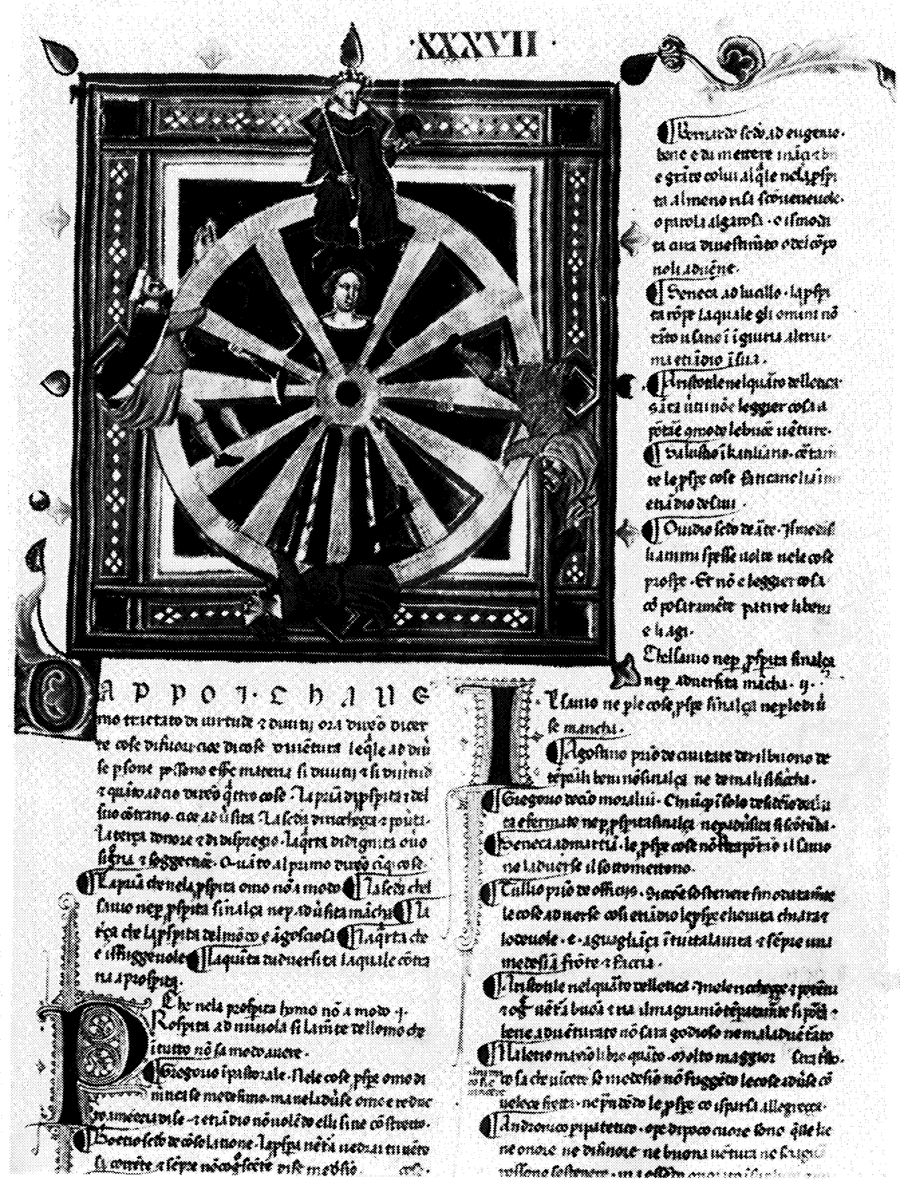
\includegraphics{include/html/images/322_1.png}

PLATE 1. \emph{Wheel of Fortune}. Codex miniature. Biblioteca Nazionale,
Florence, Italy. Courtesy of Alinari/Art Resource, New York.

\protect\hypertarget{20_ILLUSTRATIONS_FOLLOW_PAGE.xhtmlux5cux23id_3}{}{}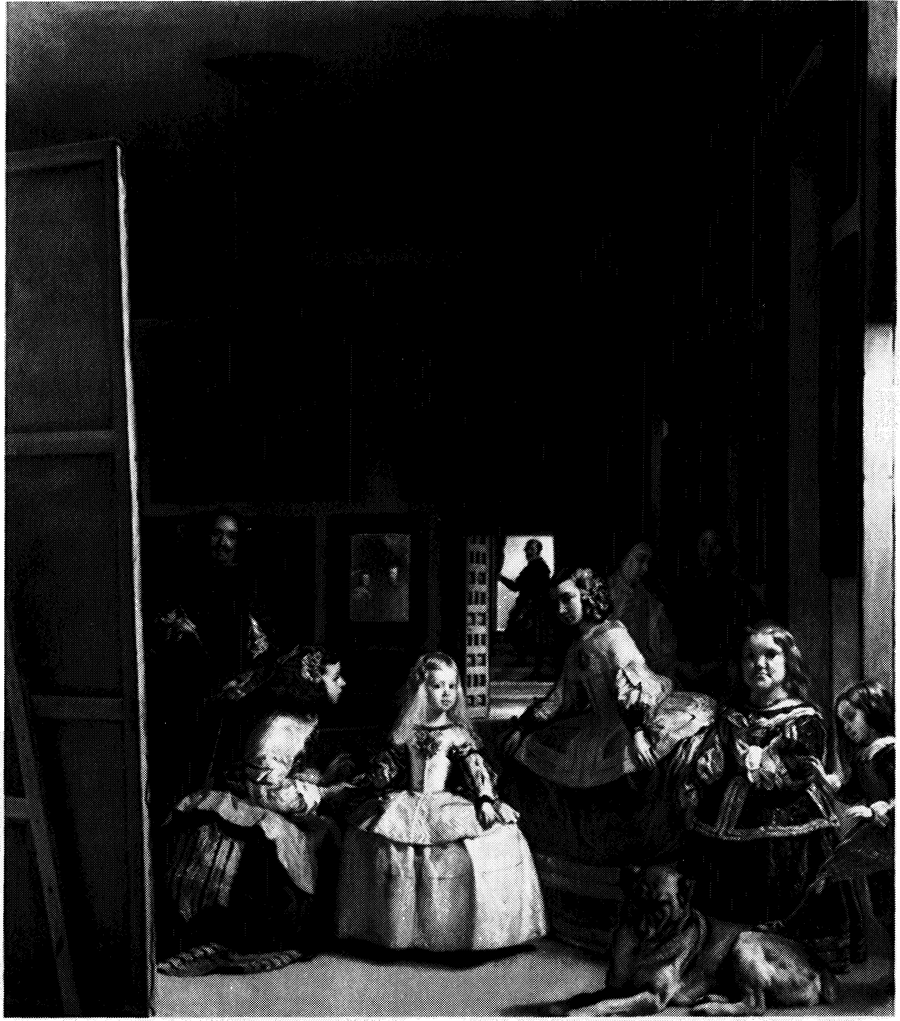
\includegraphics{include/html/images/323_1.png}

PLATE 2. Velazquez, Diego Rodriguez de Silva. \emph{The Maids of Honor}.
Prado, Madrid.

\protect\hypertarget{20_ILLUSTRATIONS_FOLLOW_PAGE.xhtmlux5cux23id_4}{}{}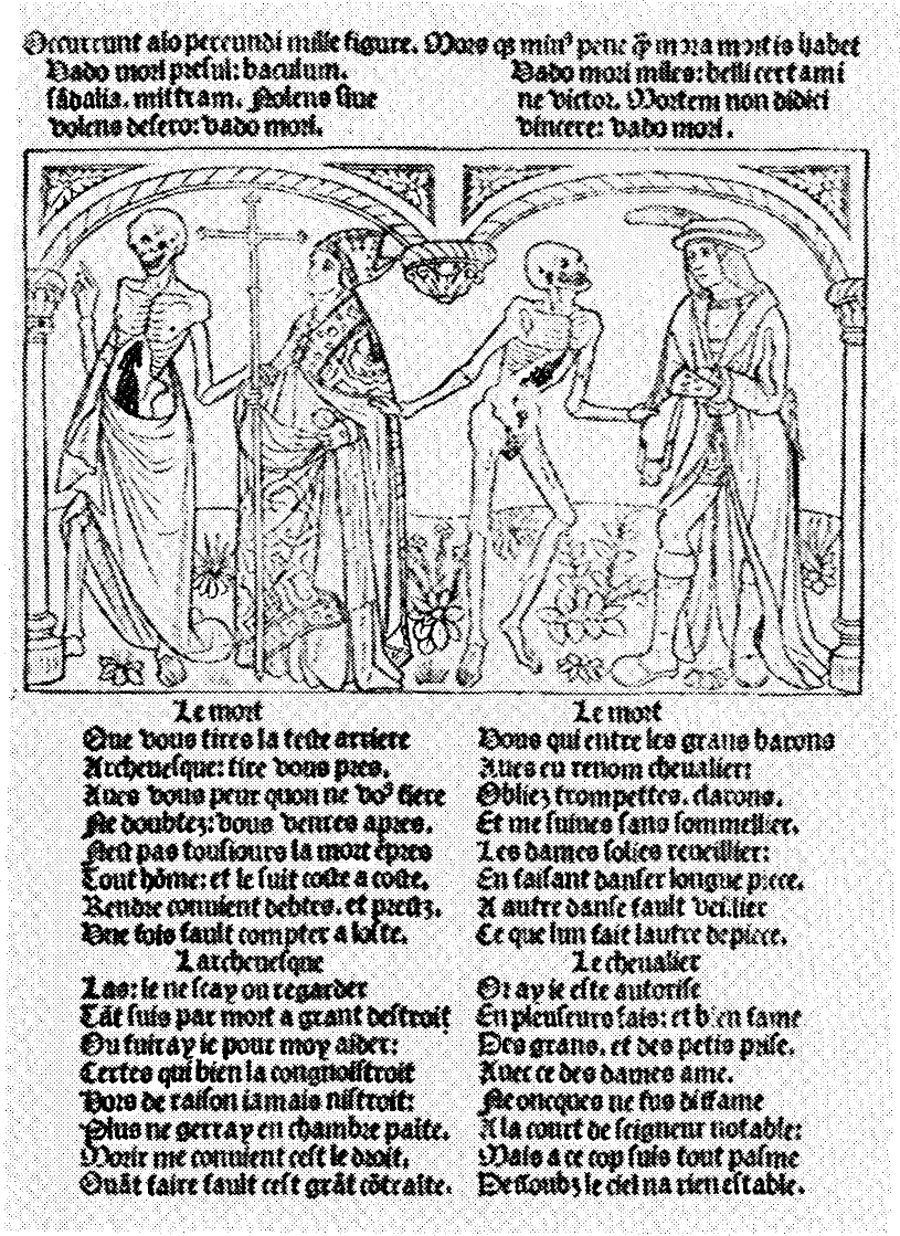
\includegraphics{include/html/images/324_1.png}

PLATE 3. Marchand, Guyot. \emph{Danse Macabre}. 1486. Bibliothèque
Nationale, Paris. Courtesy of Giraudon/Art Resource, New York.

\protect\hypertarget{20_ILLUSTRATIONS_FOLLOW_PAGE.xhtmlux5cux23id_2297}{}{}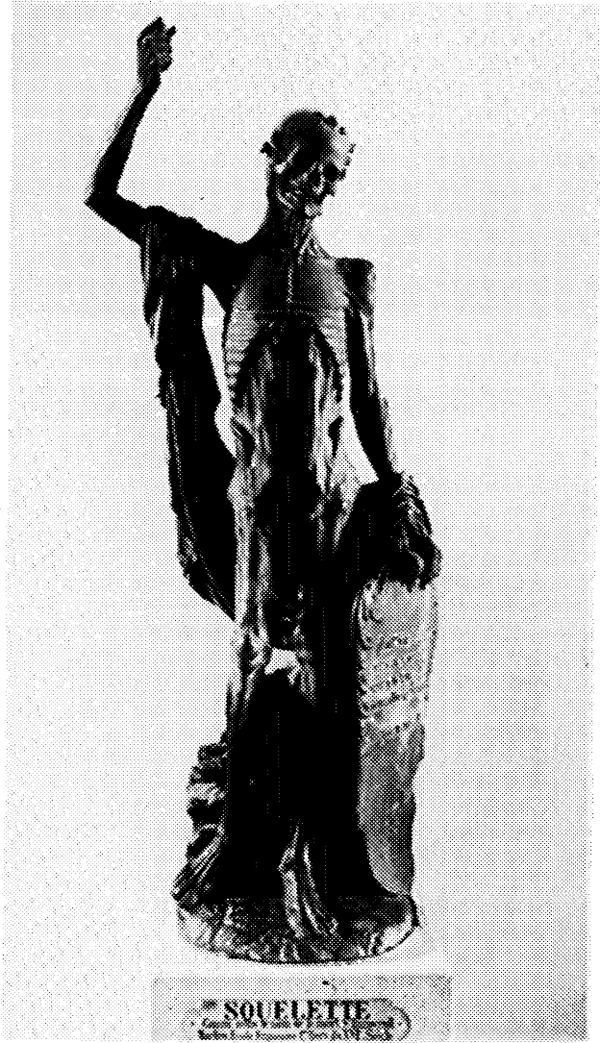
\includegraphics{include/html/images/324_2.png}

PLATE 4. French School. Figure of Death from the Cemetery of the
Innocents, Paris. 16th century. Louvre, Paris. Courtesy of Giraudon/Art
Resource, New York.

\protect\hypertarget{20_ILLUSTRATIONS_FOLLOW_PAGE.xhtmlux5cux23id_5}{}{}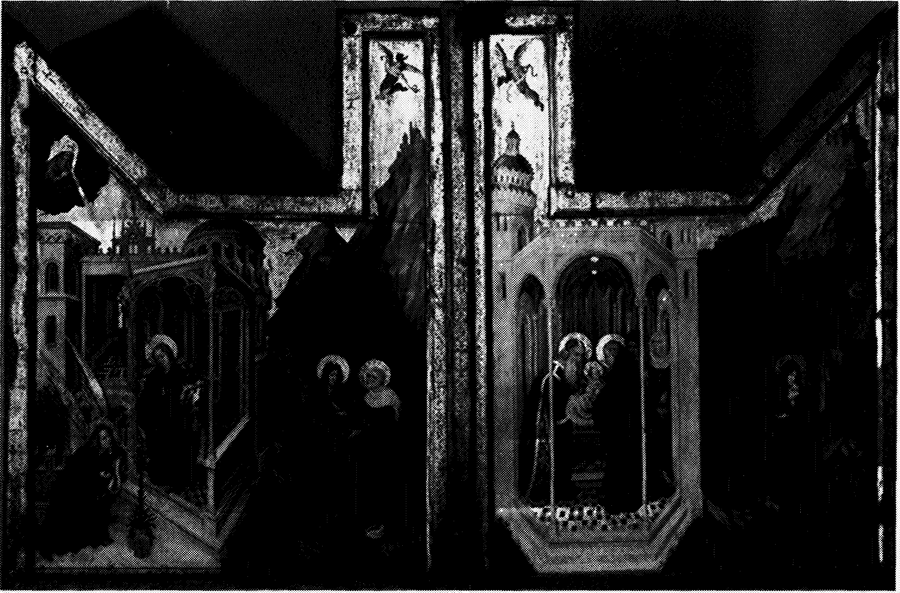
\includegraphics{include/html/images/325_1.png}

PLATE 5. Broederlam, Melchior. \emph{The Flight into Egypt}. Musée de
Beaux-Arts, Dijon.

\protect\hypertarget{20_ILLUSTRATIONS_FOLLOW_PAGE.xhtmlux5cux23id_6}{}{}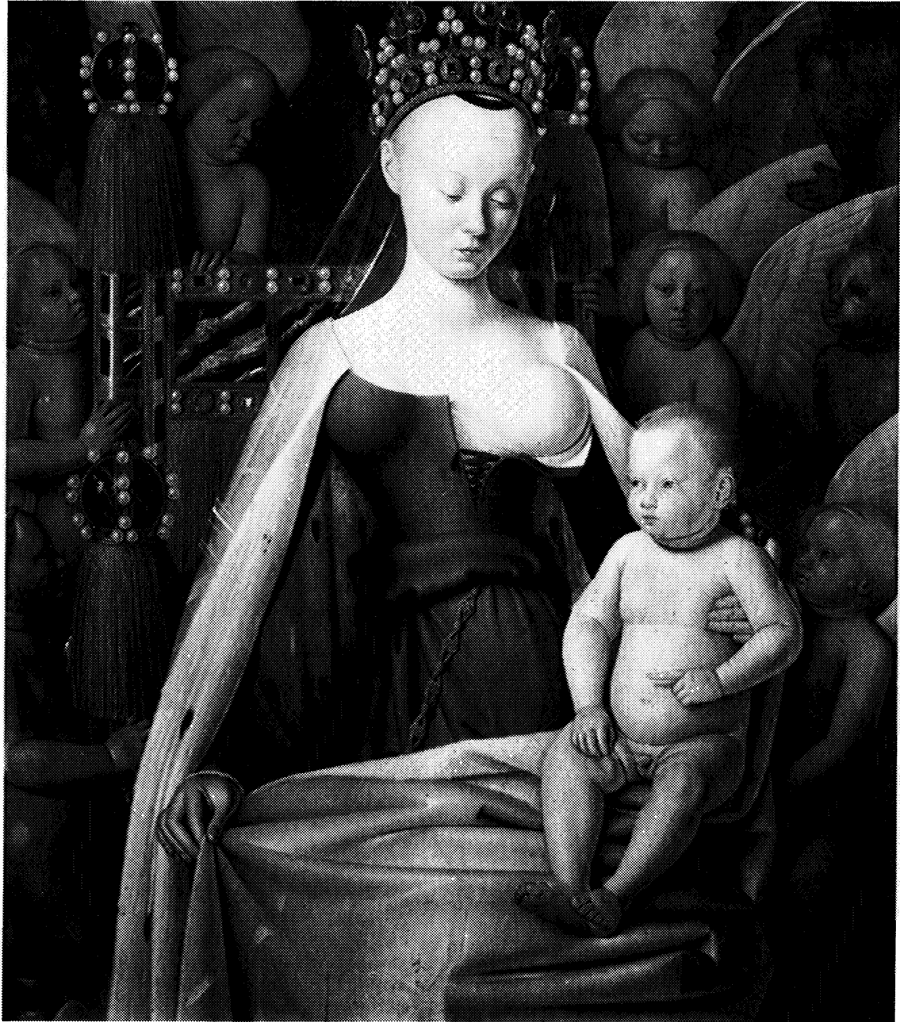
\includegraphics{include/html/images/326_1.png}

PLATE 6. Foucquet, Jean. \emph{Melun Madonna}. Koninklijk Museum,
Antwerp.

\protect\hypertarget{20_ILLUSTRATIONS_FOLLOW_PAGE.xhtmlux5cux23id_7}{}{}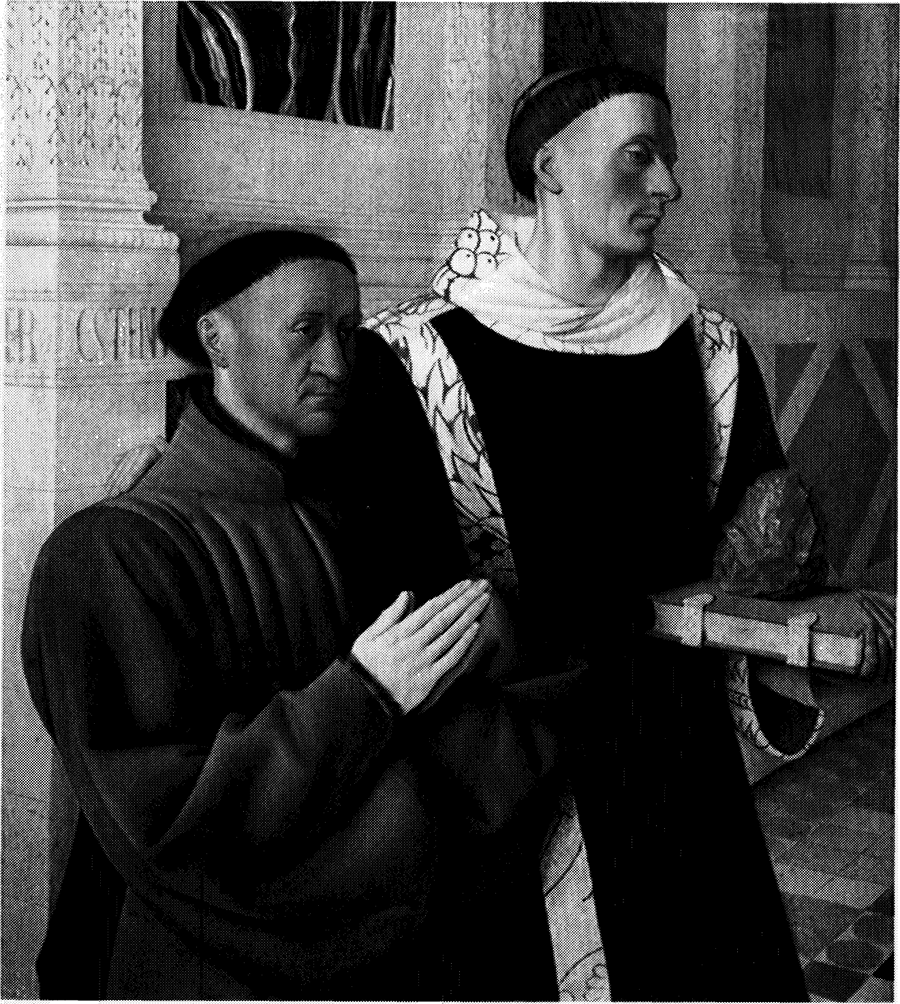
\includegraphics{include/html/images/327_1.png}

PLATE 7. Foucquet, Jean. \emph{Etienne Chevalier with St. Stephen}.
Gemaeldegalerie, Staatliche Museen, Berlin. Courtesy of Foto Marburg/Art
Resource, New York.

\protect\hypertarget{20_ILLUSTRATIONS_FOLLOW_PAGE.xhtmlux5cux23id_8}{}{}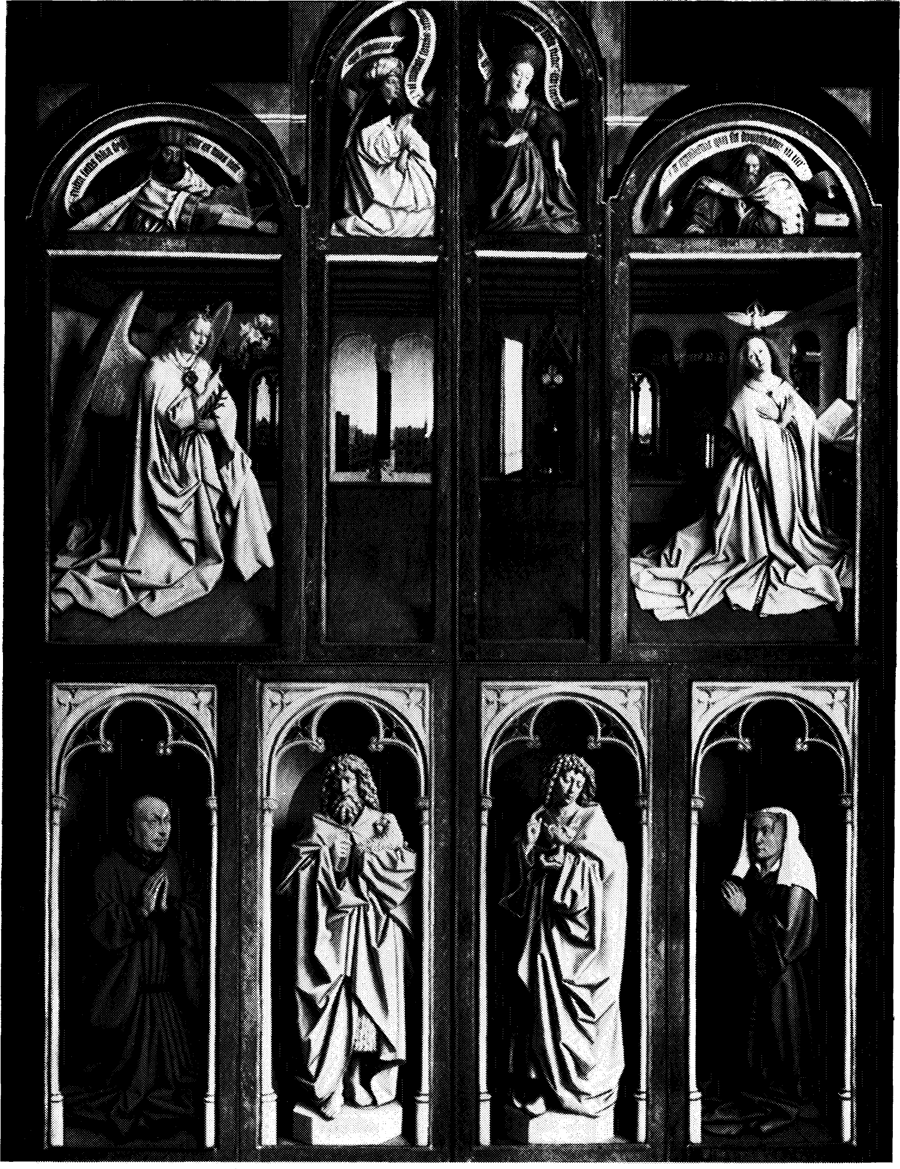
\includegraphics{include/html/images/328_1.png}

PLATE 8. Van Eyck, Jan. Ghent Altarpiece, closed. 1432. Cathedral St.
Bavo, Ghent. Courtesy of Giraudon/Art Resource, New York.

\protect\hypertarget{20_ILLUSTRATIONS_FOLLOW_PAGE.xhtmlux5cux23id_9}{}{}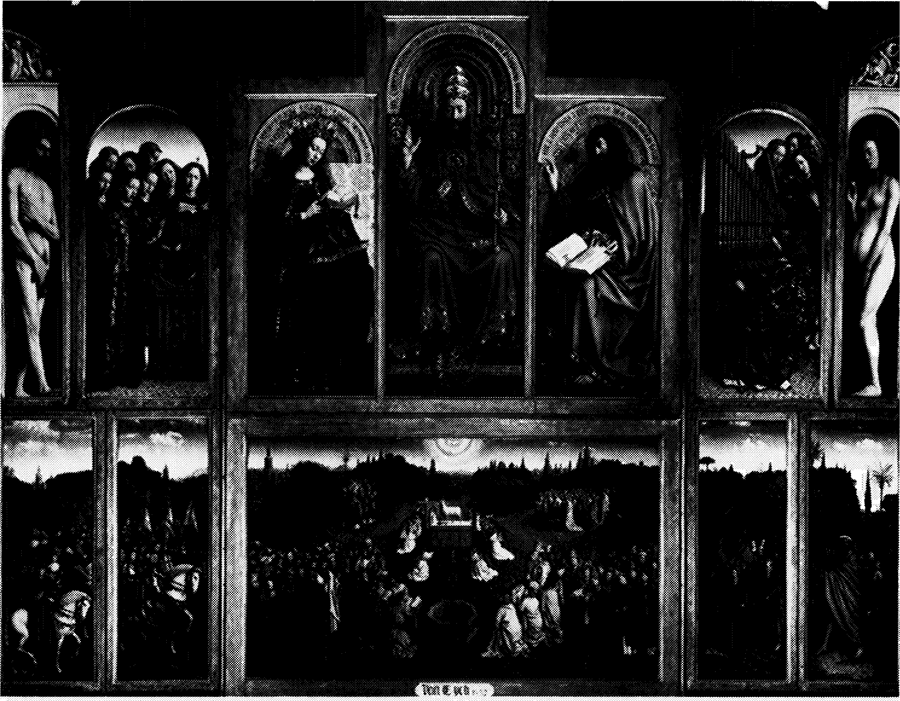
\includegraphics{include/html/images/329_1.png}

PLATE 9. Van Eyck, Jan. Ghent Altarpiece, open. 1432. Cathedral St.
Bavo, Ghent. Courtesy of Giraudon/Art Resource, New York.

\protect\hypertarget{20_ILLUSTRATIONS_FOLLOW_PAGE.xhtmlux5cux23id_10}{}{}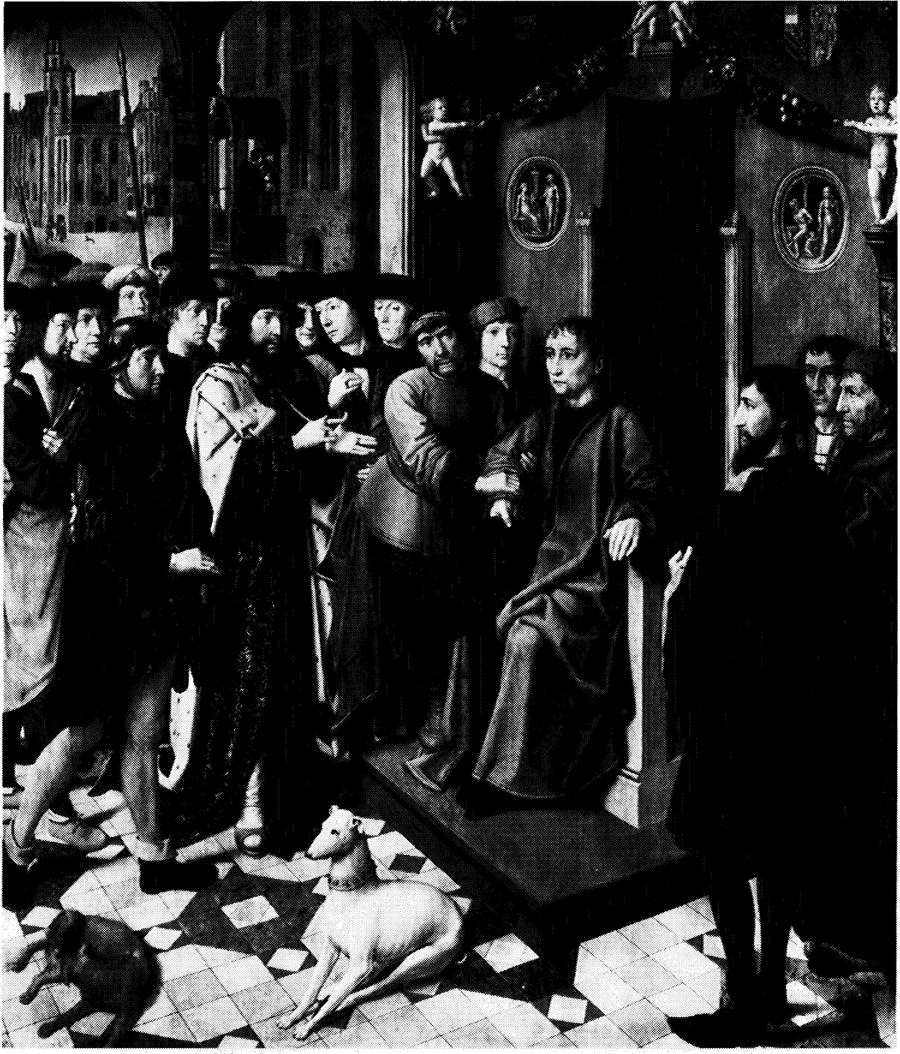
\includegraphics{include/html/images/330_1.png}

PLATE 10. David, Gerard. \emph{Judgement of Cambyses}. Municipal Museum,
Bruges. Courtesy of Alinari/Art Resource, New York.

\protect\hypertarget{20_ILLUSTRATIONS_FOLLOW_PAGE.xhtmlux5cux23id_11}{}{}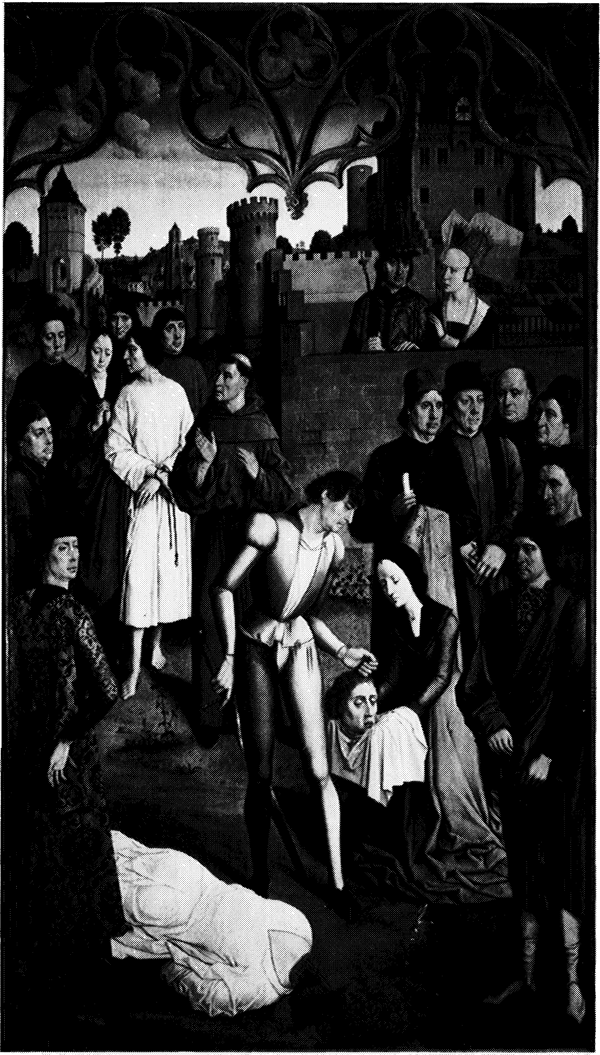
\includegraphics{include/html/images/331_1.png}

PLATE 11. Bouts, Dirk. \emph{Judgement of the Emperor Otto} (Scene 1).
Musée Royaux, Brussels.

\protect\hypertarget{20_ILLUSTRATIONS_FOLLOW_PAGE.xhtmlux5cux23id_12}{}{}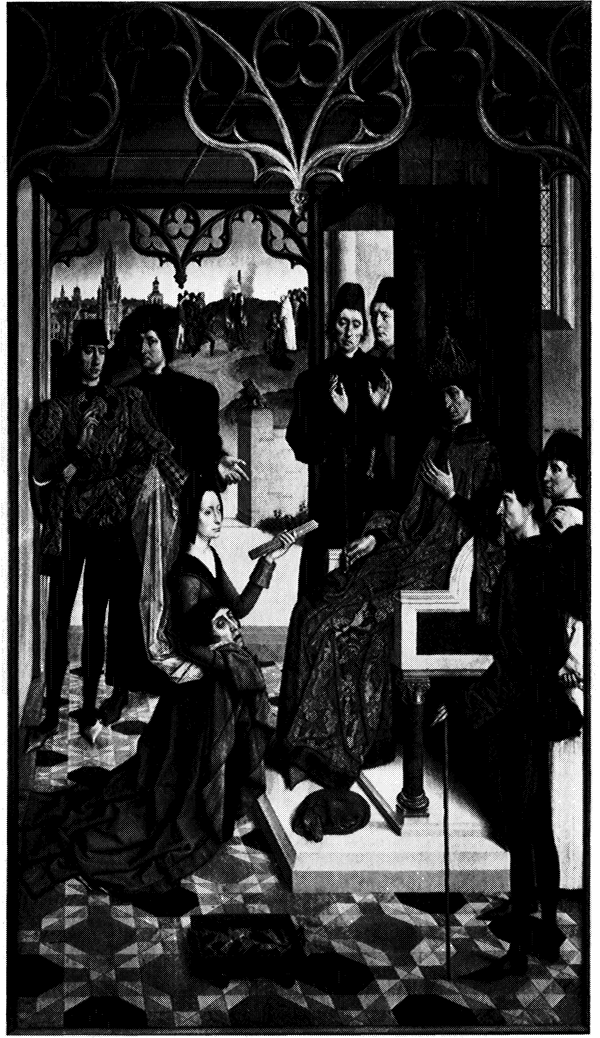
\includegraphics{include/html/images/332_1.png}

(Scene 2)

\protect\hypertarget{20_ILLUSTRATIONS_FOLLOW_PAGE.xhtmlux5cux23id_13}{}{}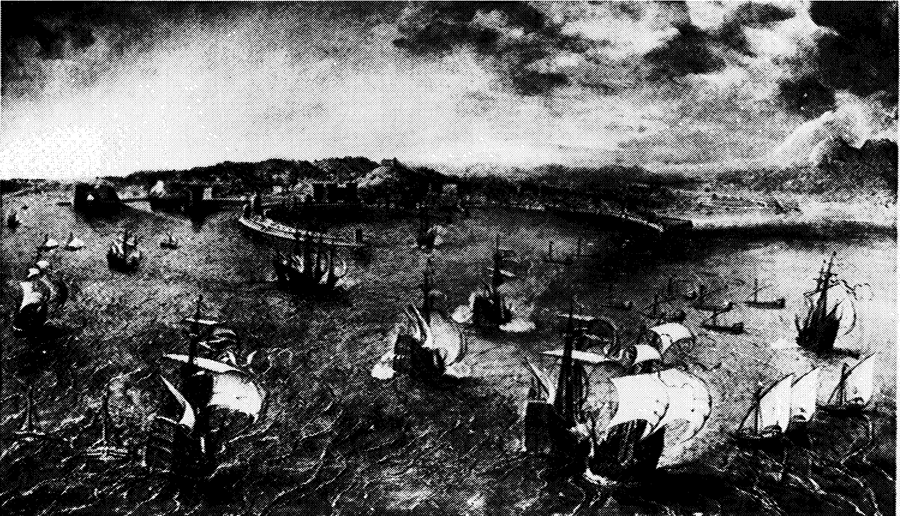
\includegraphics{include/html/images/333_1.png}

PLATE 12. Breughel, Pieter the Elder. The Old Port of Naples. Palazzo
Doria, Rome. Courtesy of Alinari/Art Resource, New York.

\protect\hypertarget{20_ILLUSTRATIONS_FOLLOW_PAGE.xhtmlux5cux23id_14}{}{}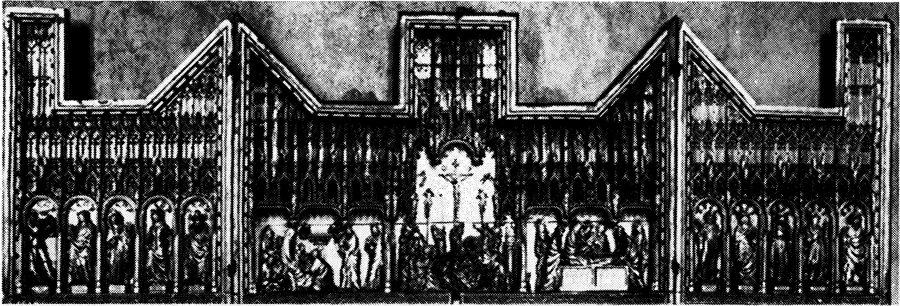
\includegraphics{include/html/images/334_1.png}

PLATE 13. Baerze, Jacques de. \emph{Retable of the Crucifixion}. Musée
des Beaux-Arts, Dijon.

\protect\hypertarget{20_ILLUSTRATIONS_FOLLOW_PAGE.xhtmlux5cux23id_2298}{}{}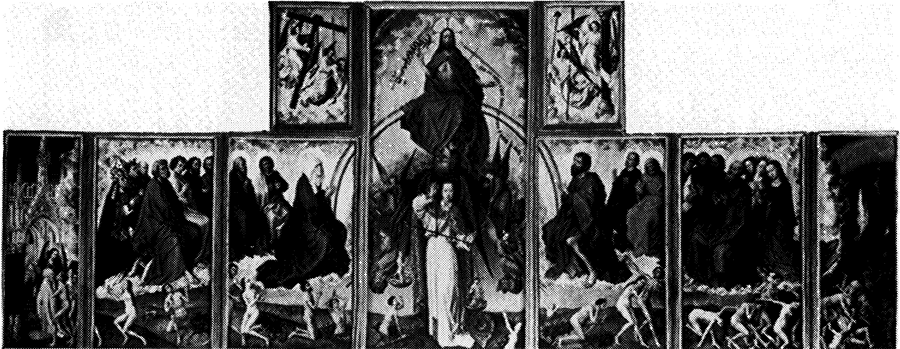
\includegraphics{include/html/images/334_2.png}

PLATE 14. Van der Weyden, Rogier. \emph{Last Judgement Altarpiece}
(open). Hotel-Dieu, Beaune, France. Courtesy of Giraudon/Art Resource,
New York.

\protect\hypertarget{20_ILLUSTRATIONS_FOLLOW_PAGE.xhtmlux5cux23id_15}{}{}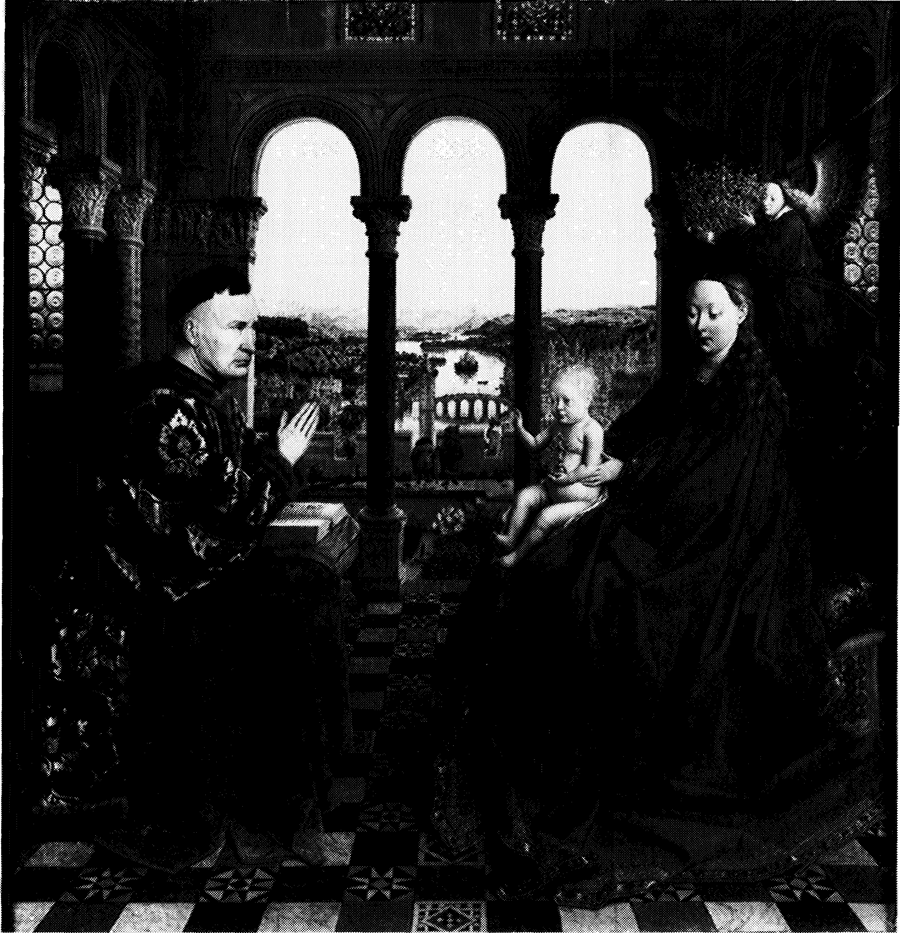
\includegraphics{include/html/images/335_1.png}

PLATE 15. Van Eyck Jan. \emph{Autun Altarpieoe}. Louvre, Paris. Cliché
des Musées Nationaux, Paris.

\protect\hypertarget{20_ILLUSTRATIONS_FOLLOW_PAGE.xhtmlux5cux23id_16}{}{}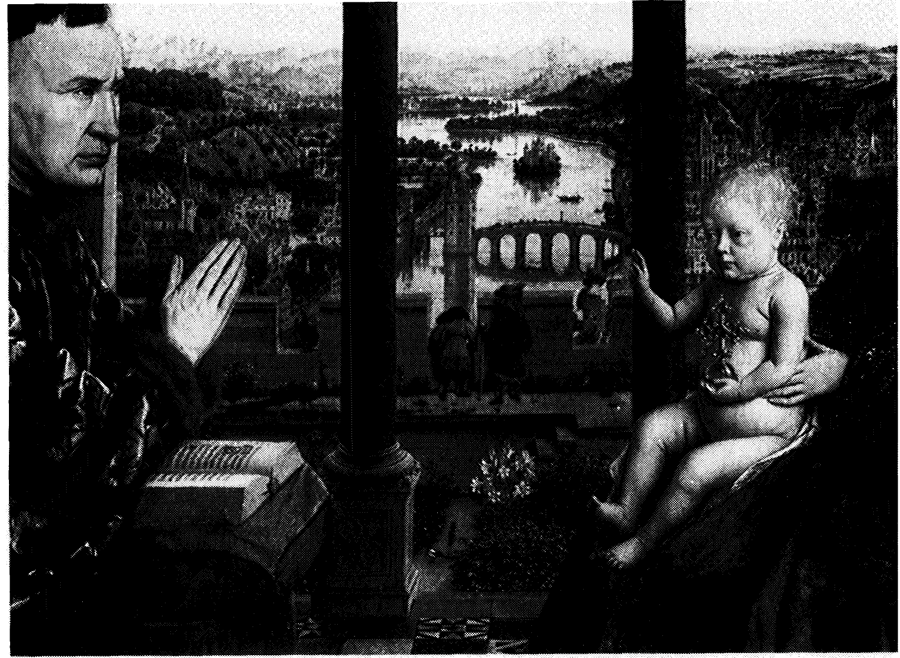
\includegraphics{include/html/images/336_1.png}

PLATE 16. Van Eyck, Jan. \emph{Autun Altarpiece}: detail of landscape in
background. Louvre, Paris. Cliché des Musées Nationaux, Paris.

\protect\hypertarget{20_ILLUSTRATIONS_FOLLOW_PAGE.xhtmlux5cux23id_17}{}{}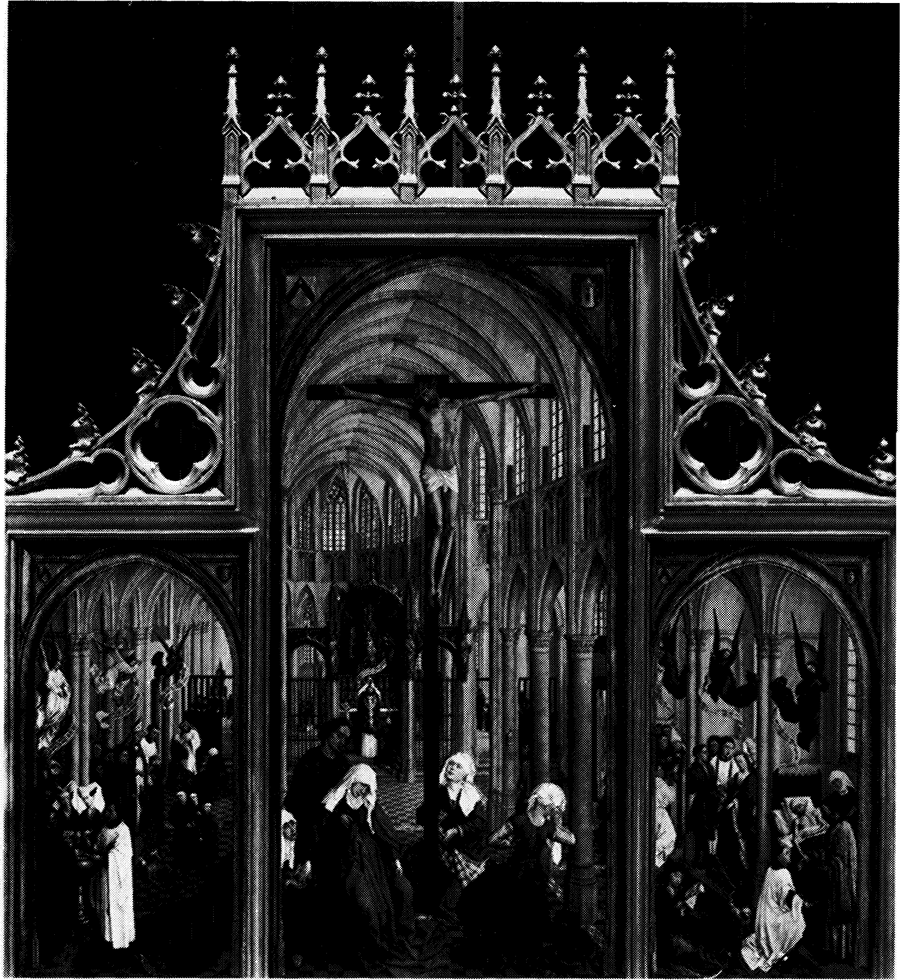
\includegraphics{include/html/images/337_1.png}

PLATE 17. Van der Weyden, Rogier. \emph{Altarpiece of the Seven
Sacraments}. Koninklijk Museum, Antwerp.

\protect\hypertarget{20_ILLUSTRATIONS_FOLLOW_PAGE.xhtmlux5cux23id_18}{}{}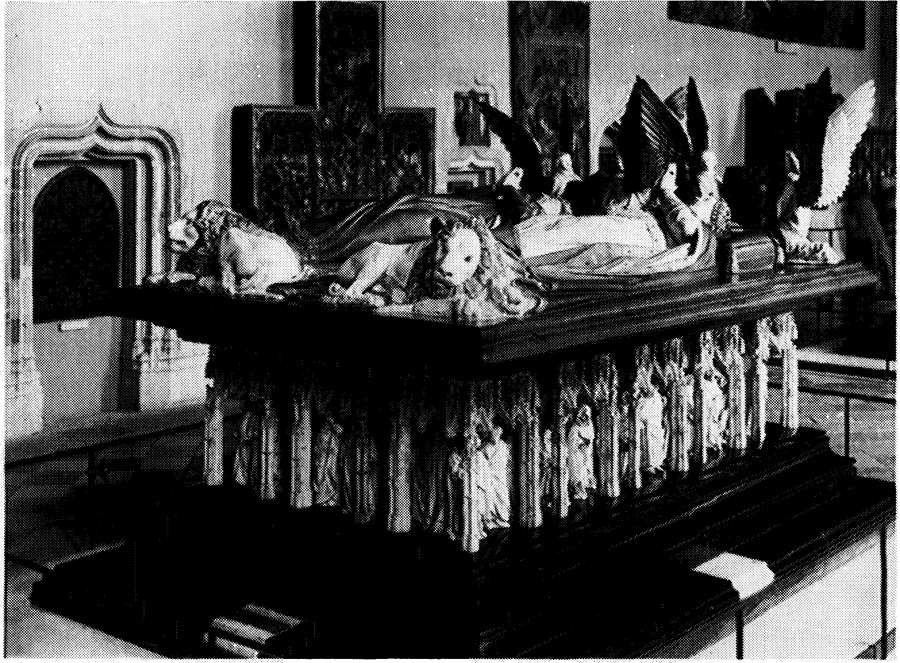
\includegraphics{include/html/images/338_1.png}

PLATE 18. Juan de la Huerta/Antoine le Moiturier. \emph{Tomb of John the
Fearless}. Musée des Beaux-Arts, Dijon.

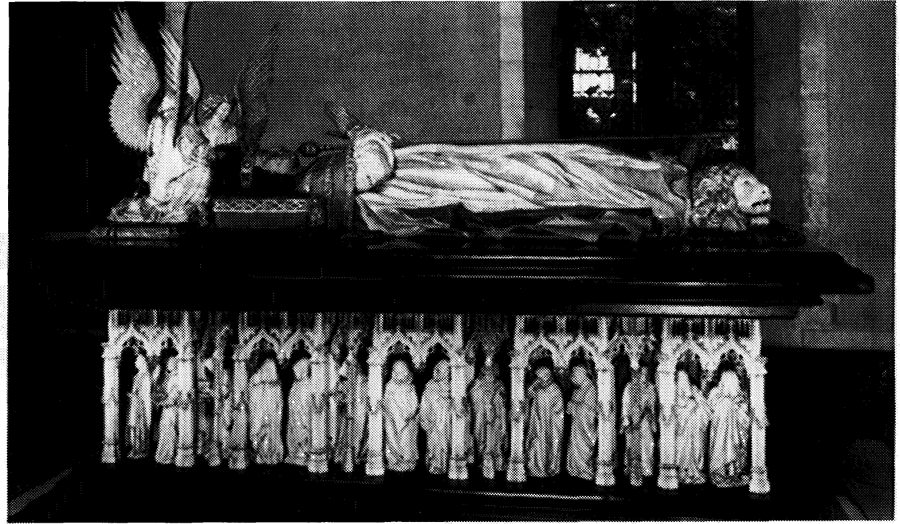
\includegraphics{include/html/images/338_2.png}

PLATE 19. Claus Sluter/Claus de Werve. \emph{Tomb of Philip the Bold}.
Musée de Beaux-Arts, Dijon.

\protect\hypertarget{20_ILLUSTRATIONS_FOLLOW_PAGE.xhtmlux5cux23id_19}{}{}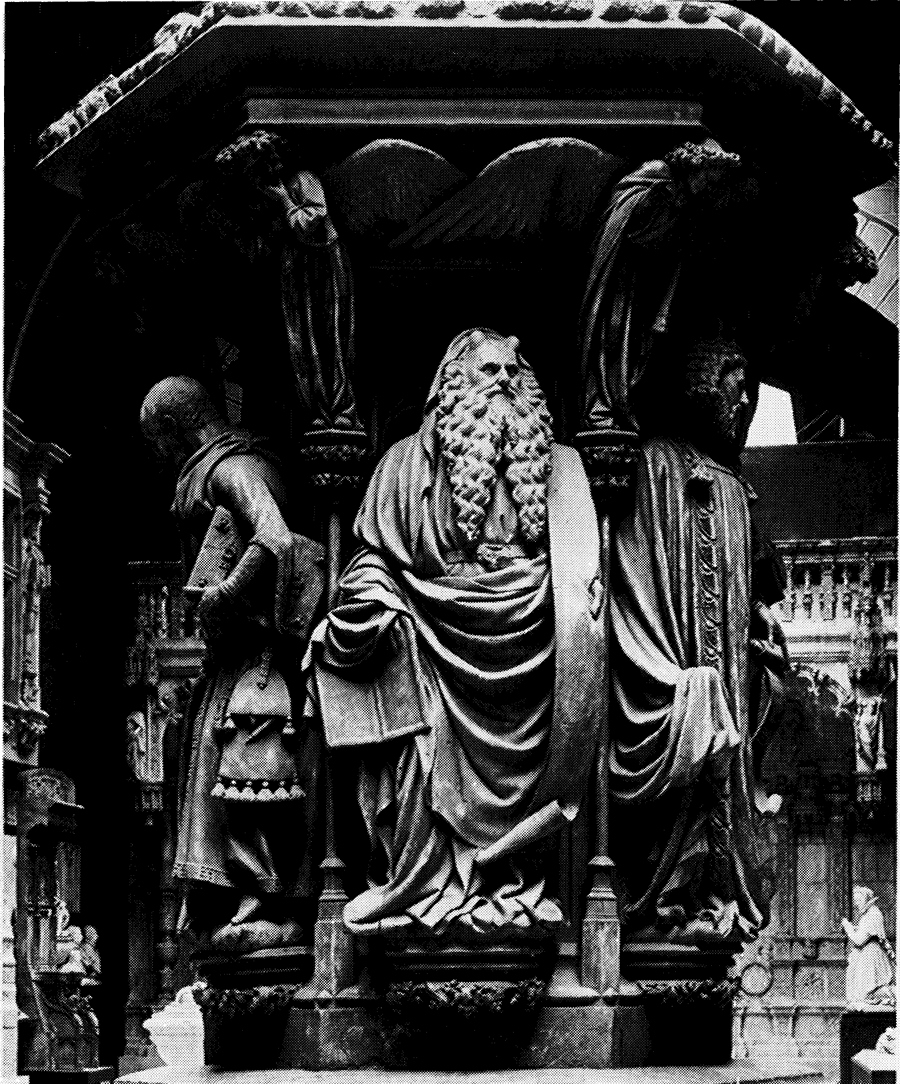
\includegraphics{include/html/images/339_1.png}

PLATE 20. Sluter, Claus. Moses from \emph{The Well of Moses}.
1395--1404. Chartreuse de Champmol, Dijon. Courtesy of Giraudon/Art
Resource, New York.

\protect\hypertarget{20_ILLUSTRATIONS_FOLLOW_PAGE.xhtmlux5cux23id_20}{}{}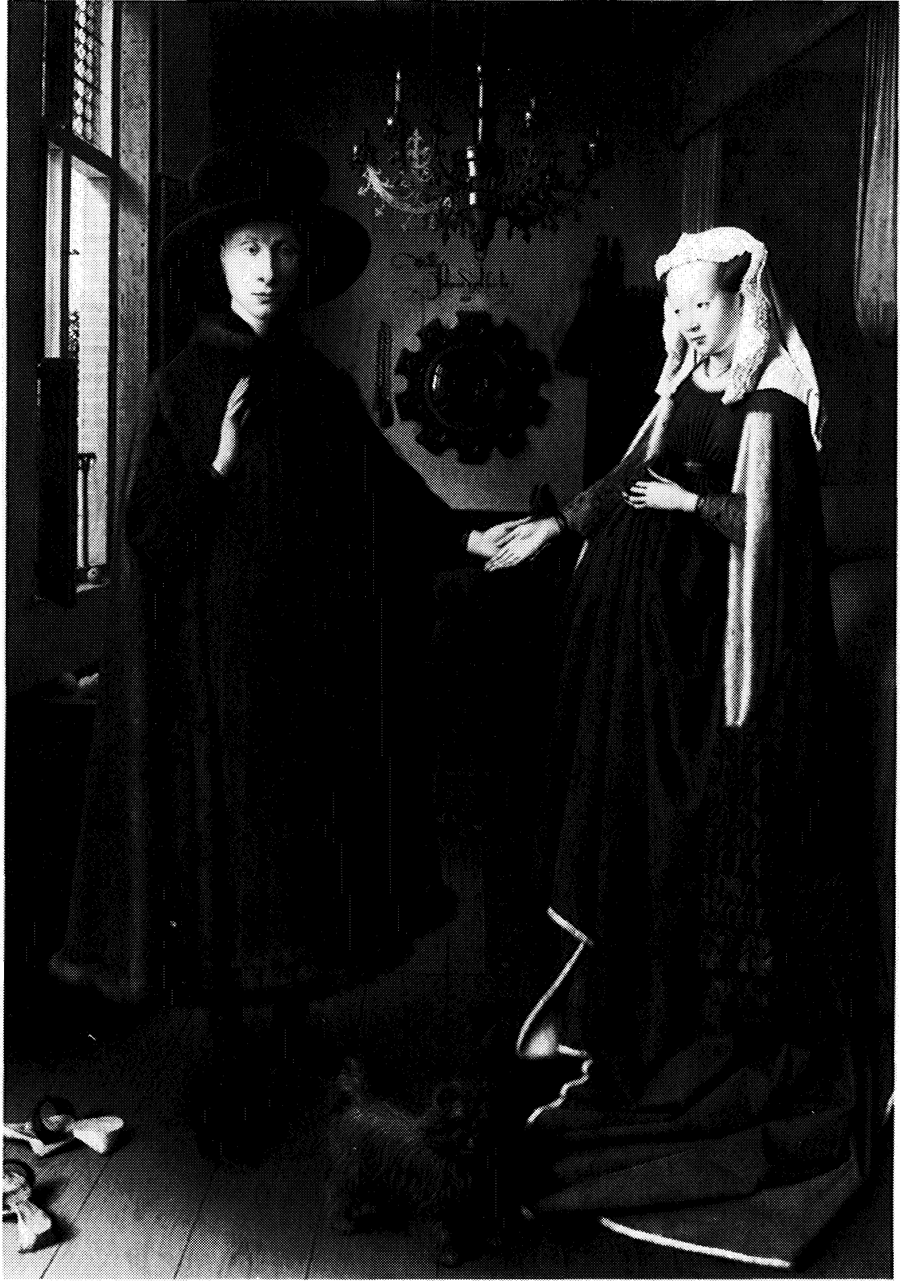
\includegraphics{include/html/images/340_1.png}

PLATE 21. Van Eyck, Jan. \emph{Wedding Portrait (Giovanni Amolfini and
Cenami Arnolfini)}. Reproduced by courtesy of the Trustees, The National
Gallery, London.

\protect\hypertarget{20_ILLUSTRATIONS_FOLLOW_PAGE.xhtmlux5cux23id_21}{}{}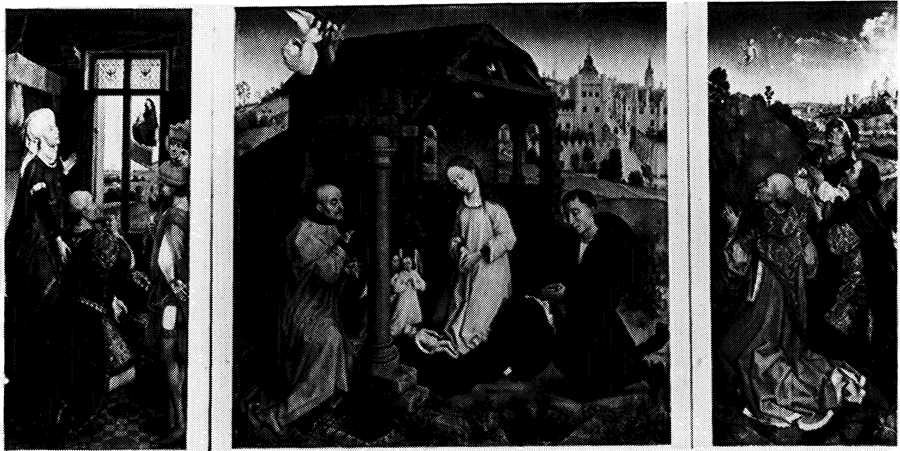
\includegraphics{include/html/images/341_1.png}

PLATE 22. Van der Weyden, Rogier. \emph{Bladelin Altarpiece}.
Gemaeldegalerie, Staatliche Museen, Berlin. Courtesy of Giraudon/Art
Resource, New York.

\protect\hypertarget{20_ILLUSTRATIONS_FOLLOW_PAGE.xhtmlux5cux23id_22}{}{}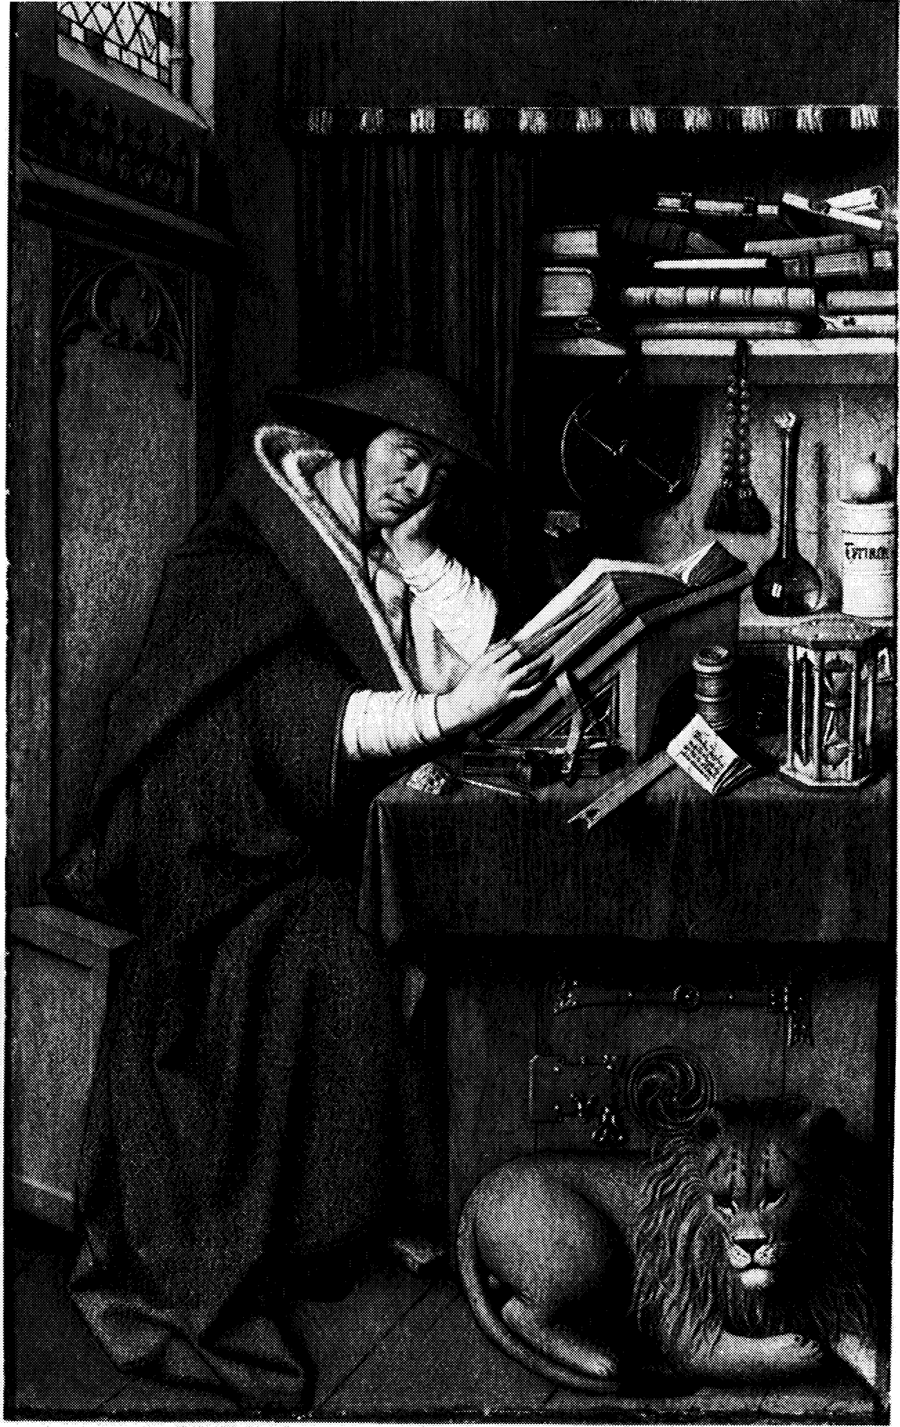
\includegraphics{include/html/images/342_1.png}

PLATE 23. Van Eyck, Jan. \emph{St. Jerome in His Study}. c. 1435. Oil on
linen paper on oak, 20.6 cm. x 13.3 cm. Accession no. 25.4. Photograph
©The Detroit Institute of Arts, 1995. City of Detroit Purchase.

\protect\hypertarget{20_ILLUSTRATIONS_FOLLOW_PAGE.xhtmlux5cux23id_23}{}{}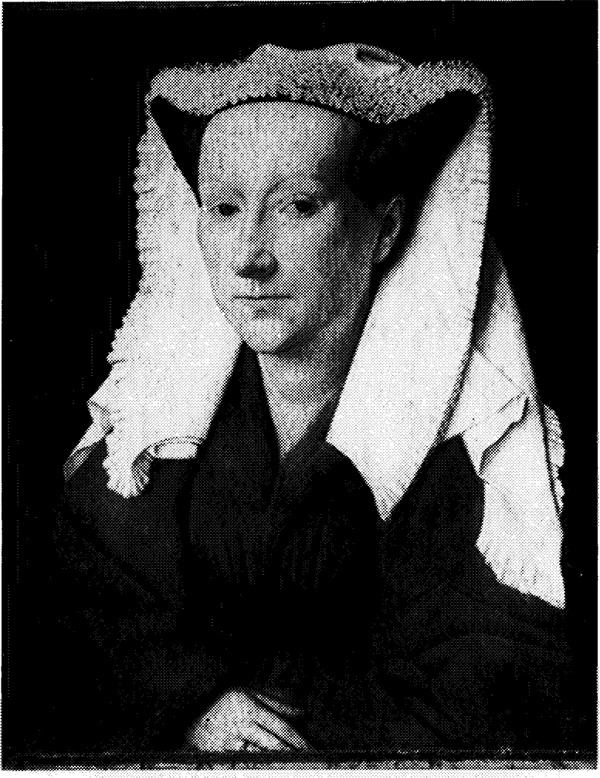
\includegraphics{include/html/images/343_1.png}

PLATE 24. Van Eyck, Jan. \emph{Margaretha van Eyck}. Municipal Museum,
Bruges. Courtesy of Foto Marburg/Art Resource, New York.

\protect\hypertarget{20_ILLUSTRATIONS_FOLLOW_PAGE.xhtmlux5cux23id_2299}{}{}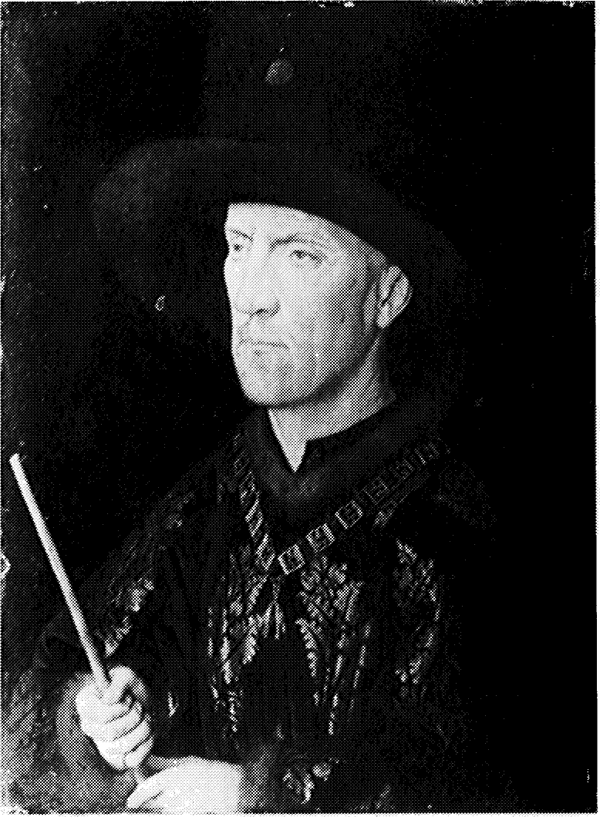
\includegraphics{include/html/images/343_2.png}

PLATE 25. Van Eyck, Jan. \emph{Baudoin de Lannoy}. Gemaeldegalerie,
Staatliche Museen, Berlin. Courtesy of Foto Marburg/Art Resource, New
York.

\protect\hypertarget{20_ILLUSTRATIONS_FOLLOW_PAGE.xhtmlux5cux23id_24}{}{}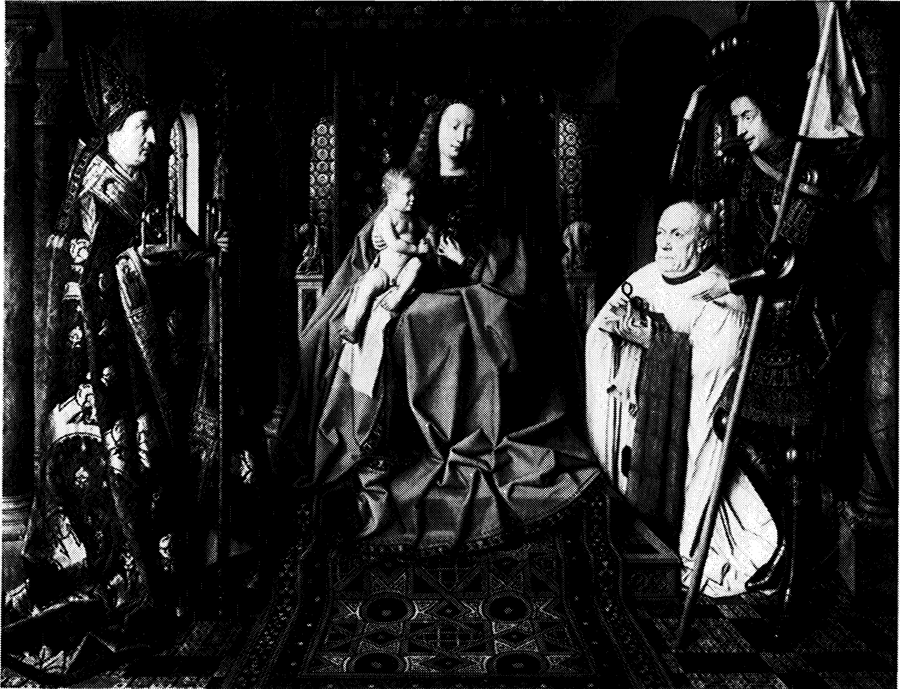
\includegraphics{include/html/images/344_1.png}

PLATE 26. Van Eyck, Jan. \emph{Madonna of Canon van der Paele}.
Municipal Museum, Bruges. Foto Marburg/Art Resource, New York.

\protect\hypertarget{20_ILLUSTRATIONS_FOLLOW_PAGE.xhtmlux5cux23id_25}{}{}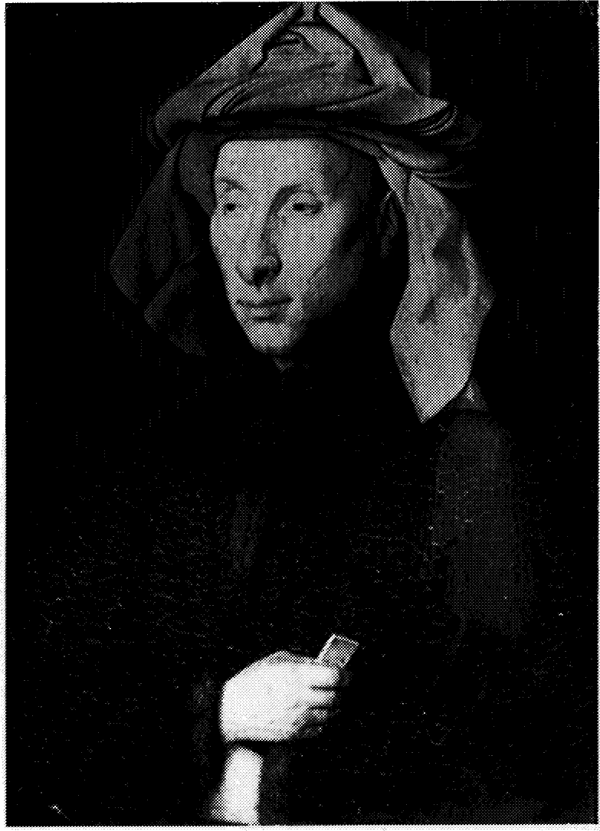
\includegraphics{include/html/images/345_1.png}

PLATE 27. Van Eyck, Jan. \emph{Giovanni Arnolfini}. Gemaeldegalerie,
Staatlich Museen, Berlin. Courtesy of Foto Marburg/Art Resource, New
York.

\protect\hypertarget{20_ILLUSTRATIONS_FOLLOW_PAGE.xhtmlux5cux23id_2300}{}{}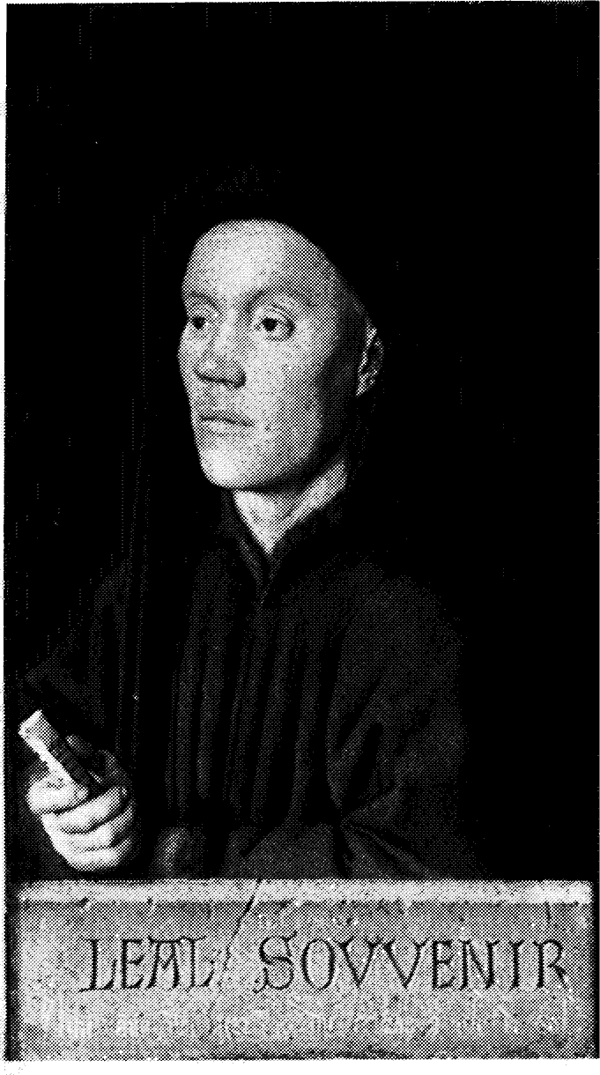
\includegraphics{include/html/images/345_2.png}

PLATE 28. Van Eyck, Jan. \emph{Leal Souvenier}. Reproduced by courtesy
of the Trustees, National Gallery, London.

\protect\hypertarget{20_ILLUSTRATIONS_FOLLOW_PAGE.xhtmlux5cux23id_26}{}{}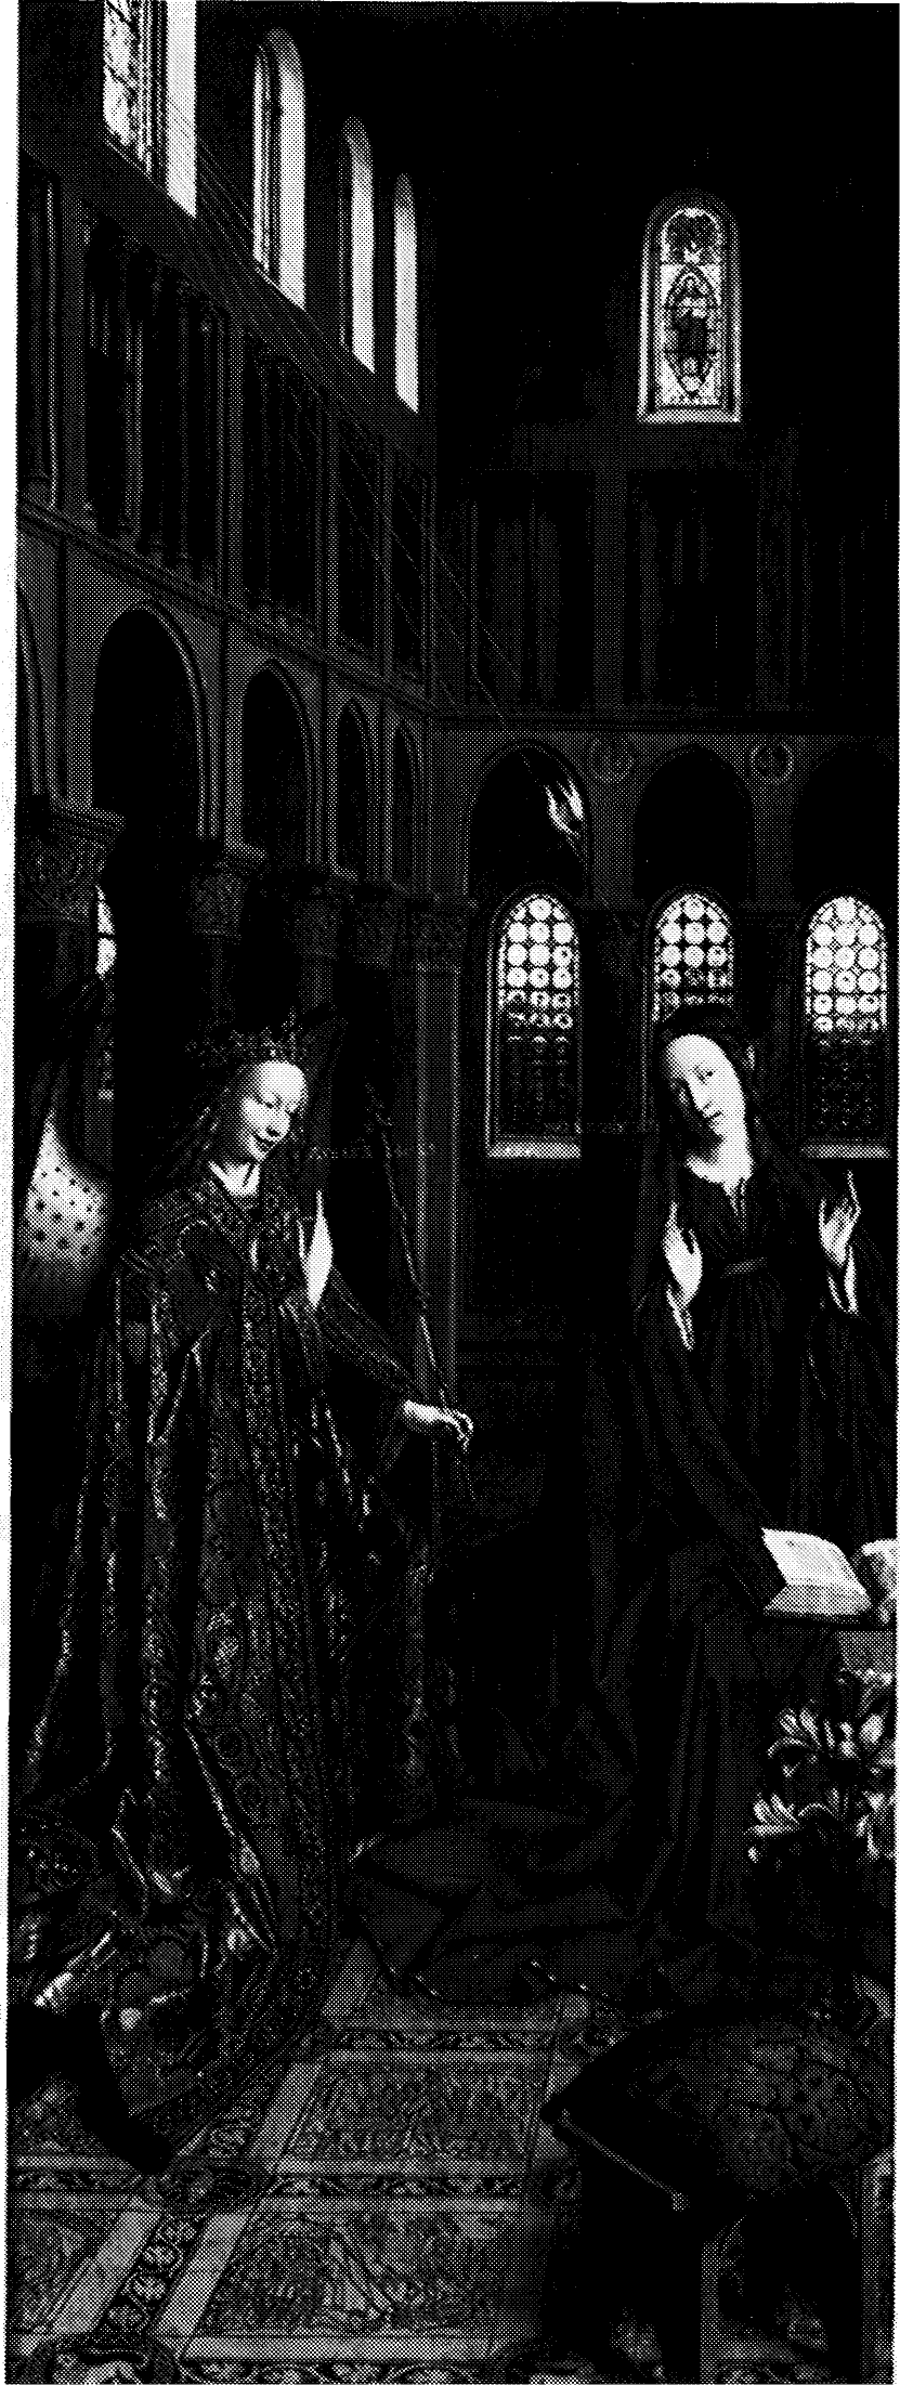
\includegraphics{include/html/images/346_1.png}

PLATE 29 (opposite). Van Eyck, Jan. \emph{Annunciation}. Andrew W.
Mellon Collection, © 1994 Board of Trustees, National Gallery of Art,
Washington, D.C.

\protect\hypertarget{20_ILLUSTRATIONS_FOLLOW_PAGE.xhtmlux5cux23id_27}{}{}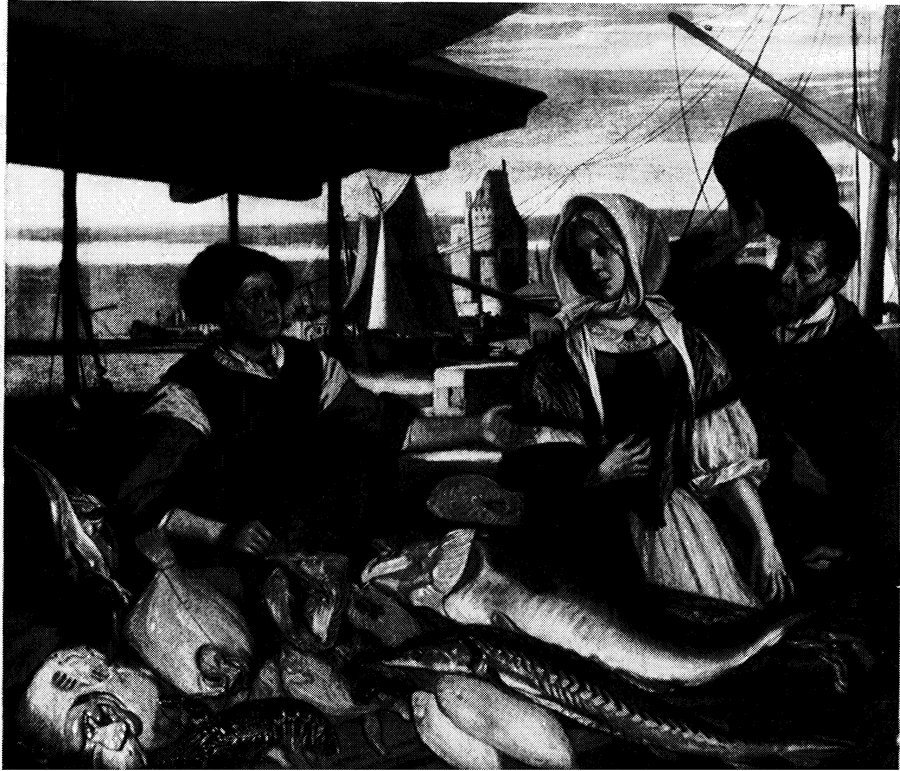
\includegraphics{include/html/images/347_1.png}

PLATE 30. De Witte, Emmanuel. \emph{The Fishmonger's Stall}. Courtesy of
Museum Boymans-van Beuningen, Rotterdam.

\protect\hypertarget{20_ILLUSTRATIONS_FOLLOW_PAGE.xhtmlux5cux23id_28}{}{}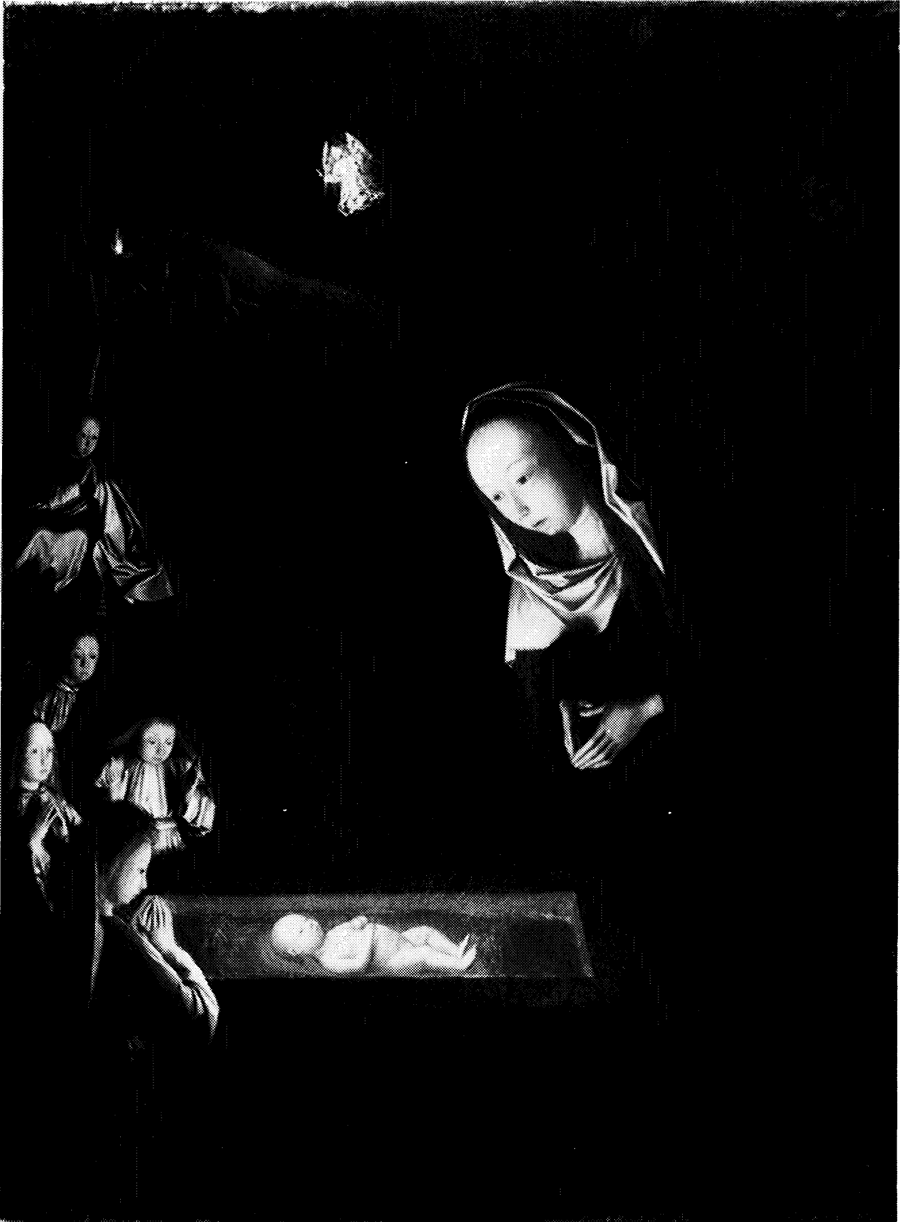
\includegraphics{include/html/images/348_1.png}

PLATE 31. Sint Jans, Geertgen tot. \emph{Nativity}. Reproduced by
courtesy of the Trustees, The National Gallery, London.

\protect\hypertarget{20_ILLUSTRATIONS_FOLLOW_PAGE.xhtmlux5cux23id_29}{}{}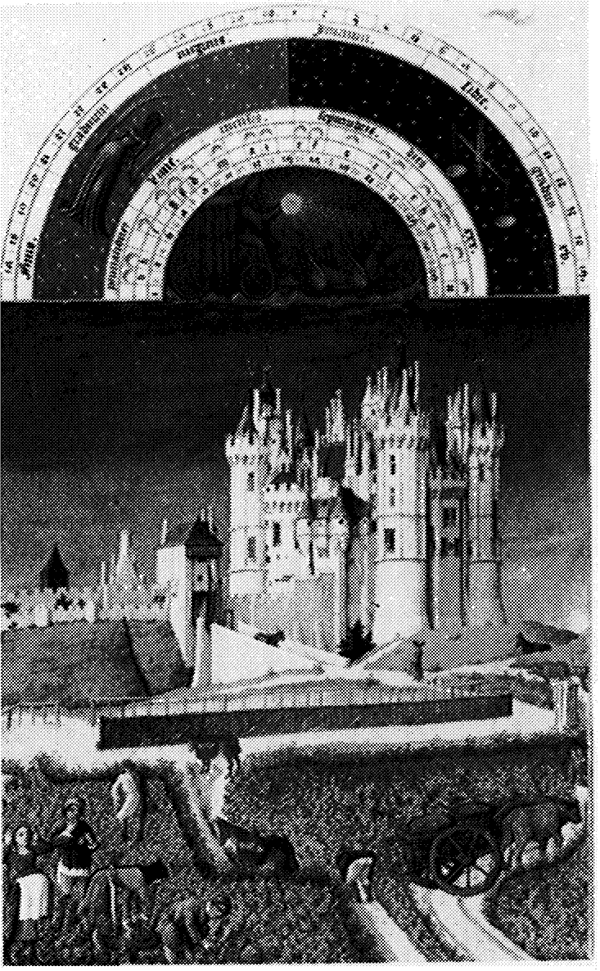
\includegraphics{include/html/images/349_1.png}

PLATE 32. Limburg Brothers. \emph{September (Grape Harvest)}. Calendar
page from the manuscript \emph{Très Riches Heures du Duc de Berry}.
Musée Conde, Chantilly. Courtesy of Giraudon/Art Resource, New York.

\protect\hypertarget{20_ILLUSTRATIONS_FOLLOW_PAGE.xhtmlux5cux23id_2301}{}{}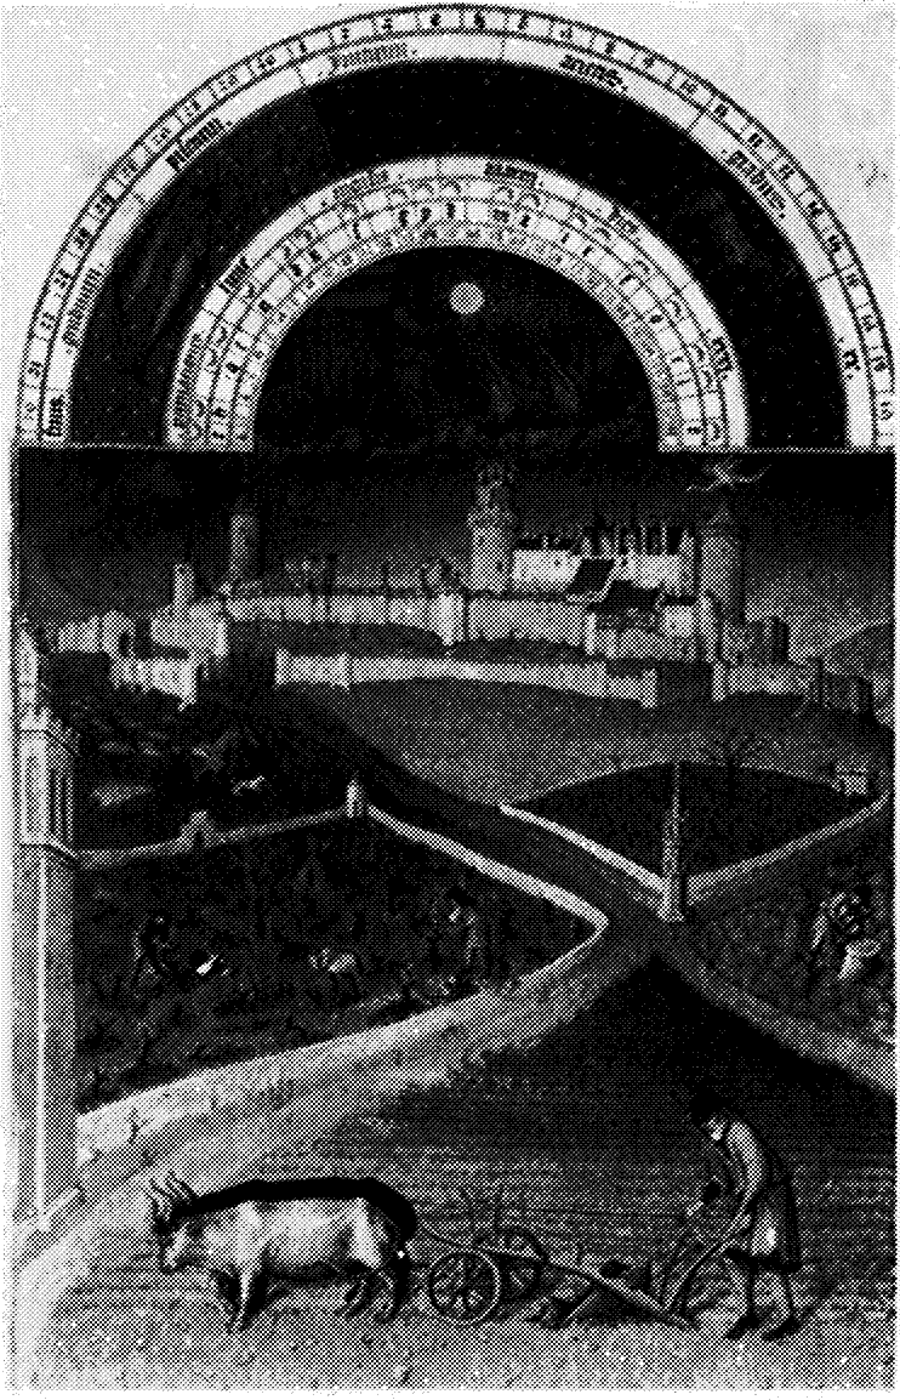
\includegraphics{include/html/images/349_2.png}

PLATE 33. Limburg Brothers. \emph{March}. Calendar page from \emph{Très
Riches Heures du Duc de Berry}. Musée Conde, Chantilly. Courtesy of
Giraudon/Art Resource, New York.

\protect\hypertarget{20_ILLUSTRATIONS_FOLLOW_PAGE.xhtmlux5cux23id_30}{}{}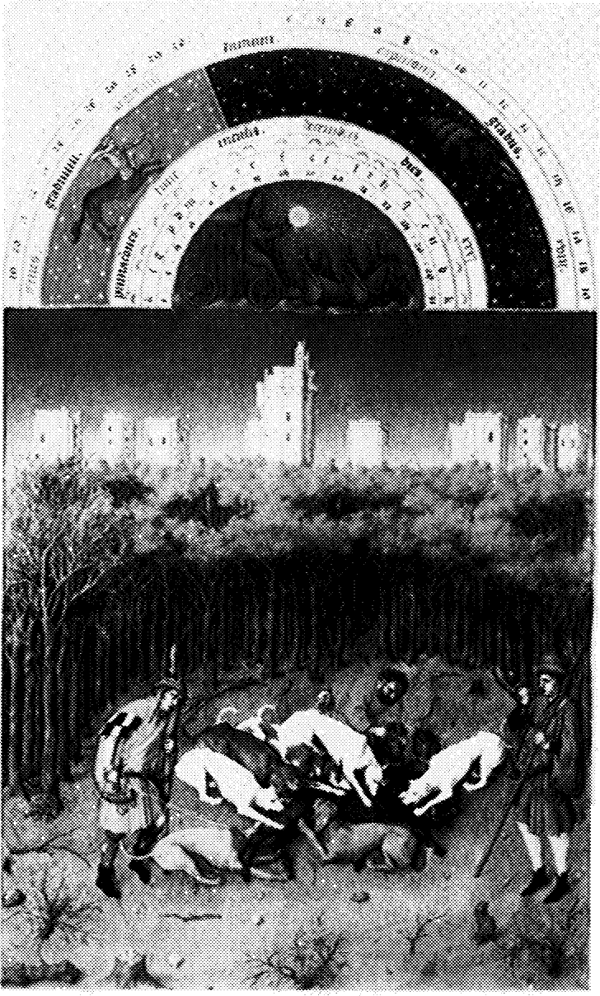
\includegraphics{include/html/images/350_1.png}

PLATE 34. Limburg Brothers. \emph{December}. Calendar page from
\emph{Très Riches Heures du Duc de Berry}. Musée Conde, Chantilly.
Courtesy of Giraudon/Art Resource, New York.

\protect\hypertarget{20_ILLUSTRATIONS_FOLLOW_PAGE.xhtmlux5cux23id_2302}{}{}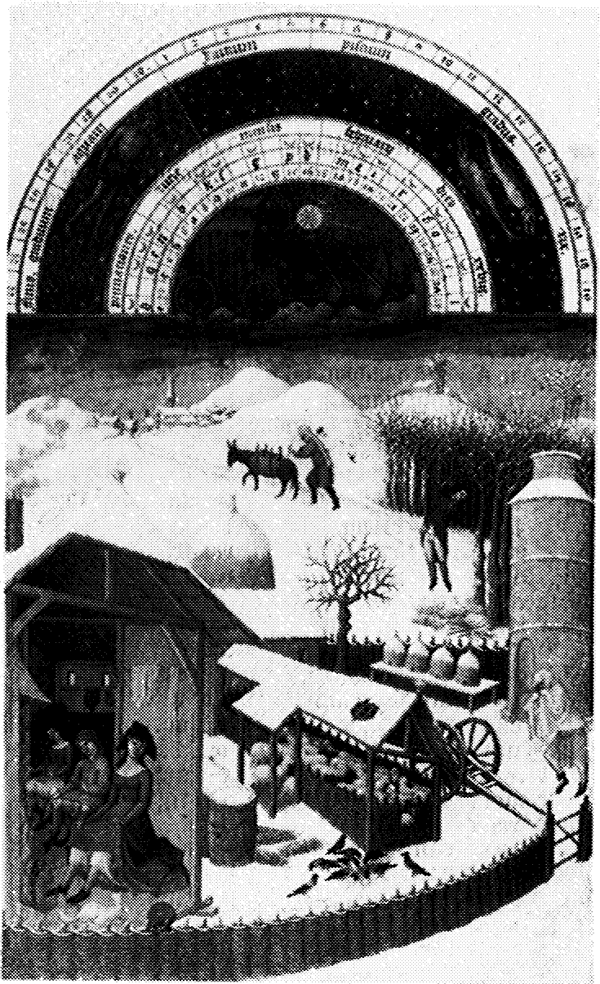
\includegraphics{include/html/images/350_2.png}

PLATE 35. Limburg Brothers. \emph{February}. Calendar page from
\emph{Très Riches Heures du Duc de Berry}. Musée Conde, Chantilly.
Courtesy of Giraudon/Art Resource, New York.

\protect\hypertarget{20_ILLUSTRATIONS_FOLLOW_PAGE.xhtmlux5cux23id_31}{}{}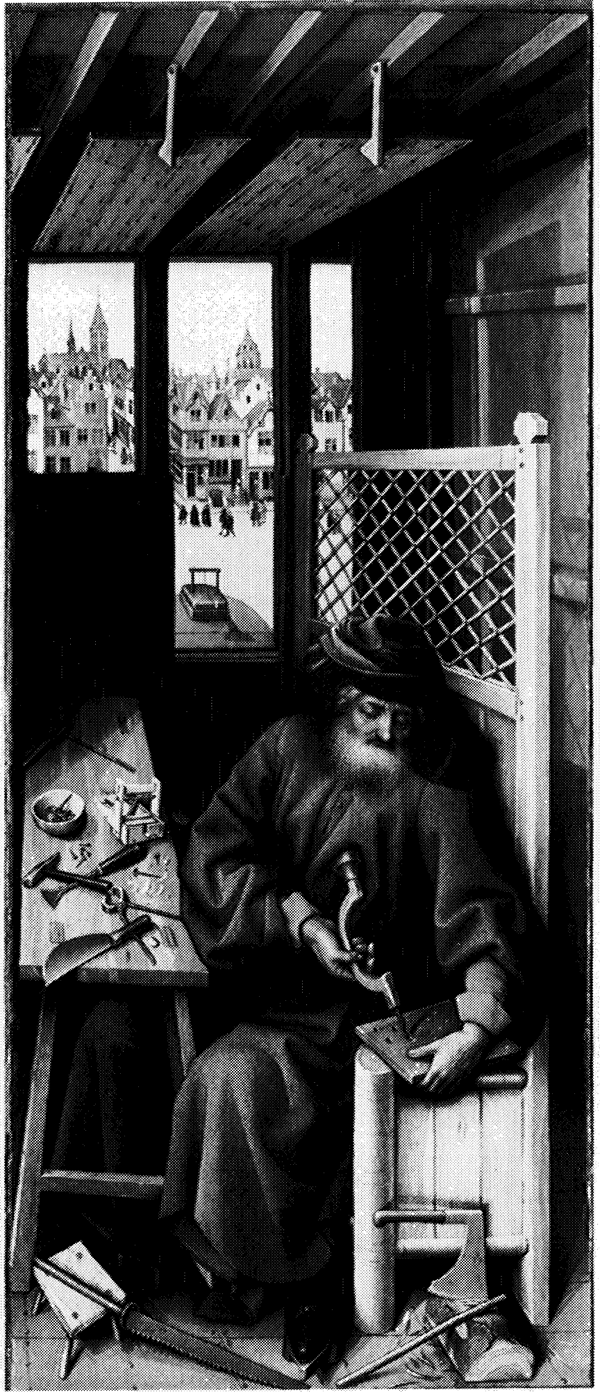
\includegraphics{include/html/images/351_1.png}

PLATE 36. Campin, Robert (Master of Flémalle). \emph{Annunciation}
(right panel). All rights reserved. The Metropolitan Museum of Art.

\protect\hypertarget{20_ILLUSTRATIONS_FOLLOW_PAGE.xhtmlux5cux23id_32}{}{}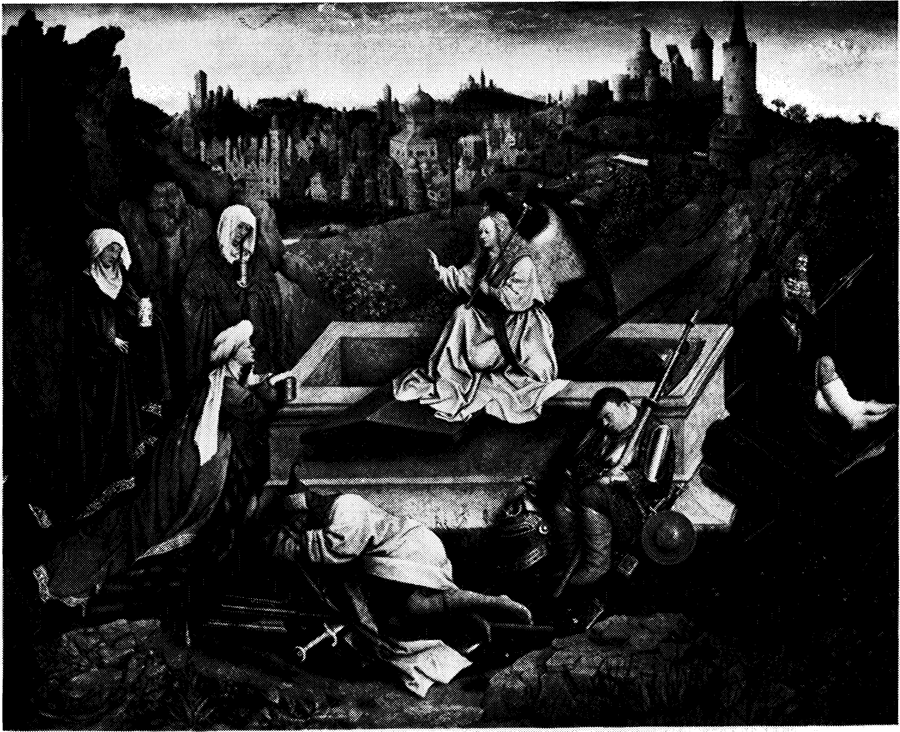
\includegraphics{include/html/images/352_1.png}

PLATE 37. Van Eyck, Hubert and Jan. \emph{The Three Marys at the Open
Sepulchre}. Museum Boymans-van Beuningen, Rotterdam.

\protect\hypertarget{20_ILLUSTRATIONS_FOLLOW_PAGE.xhtmlux5cux23id_33}{}{}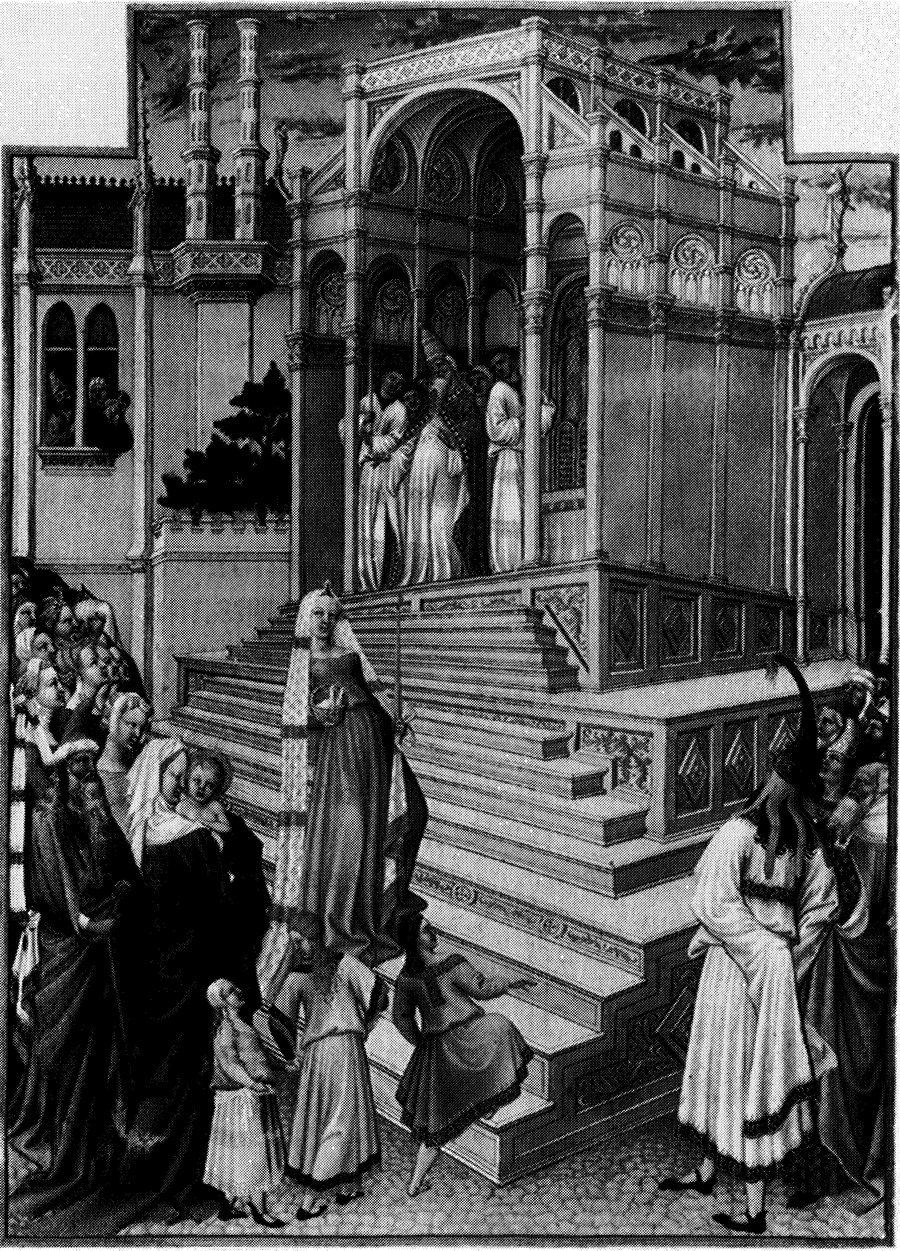
\includegraphics{include/html/images/353_1.png}

PLATE 38. Limburg Brothers. \emph{Purification}. From \emph{Très Riches
Heures du Duc de Berry}. Musée Conde, Chantilly. Courtesy of
Giraudon/Art Resource, New York.

\protect\hypertarget{20_ILLUSTRATIONS_FOLLOW_PAGE.xhtmlux5cux23id_34}{}{}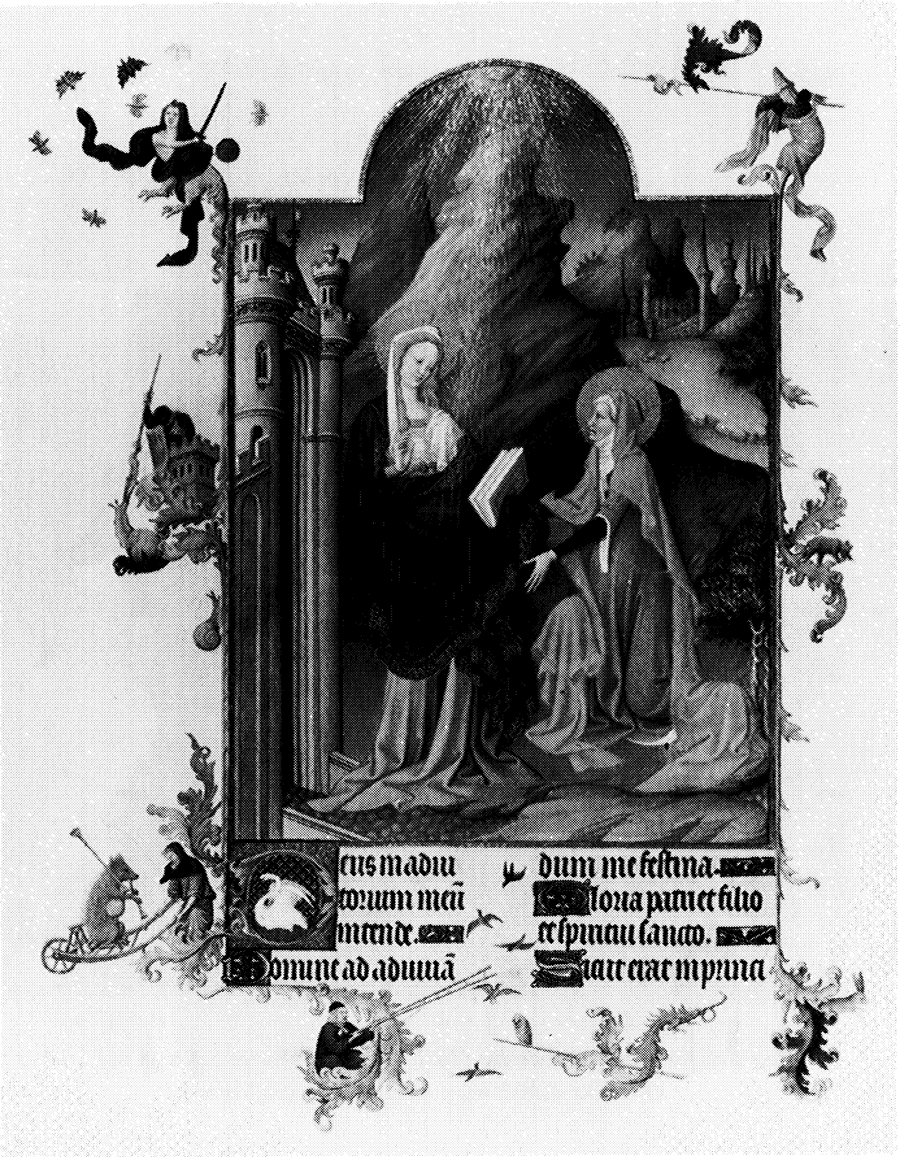
\includegraphics{include/html/images/354_1.png}

PLATE 39. Limburg Brothers. \emph{Visitation}. From \emph{Très Riches
Heures du Duc de Berry}. Musée Conde, Chantilly. Courtesy of
Giraudon/Art Resource, New York.

\protect\hypertarget{20_ILLUSTRATIONS_FOLLOW_PAGE.xhtmlux5cux23id_35}{}{}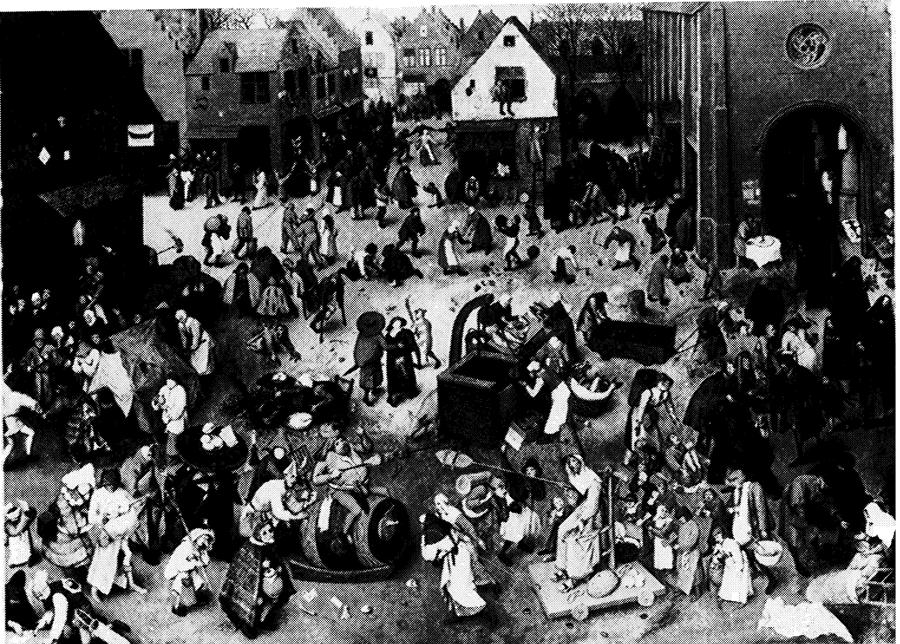
\includegraphics{include/html/images/355_1.png}

PLATE 40. Breughel, Pieter the Elder. \emph{The Battle between Carnival
and Lent}. Courtesy of Kunsthistorisches Museum, Vienna.

\protect\hypertarget{20_ILLUSTRATIONS_FOLLOW_PAGE.xhtmlux5cux23id_36}{}{}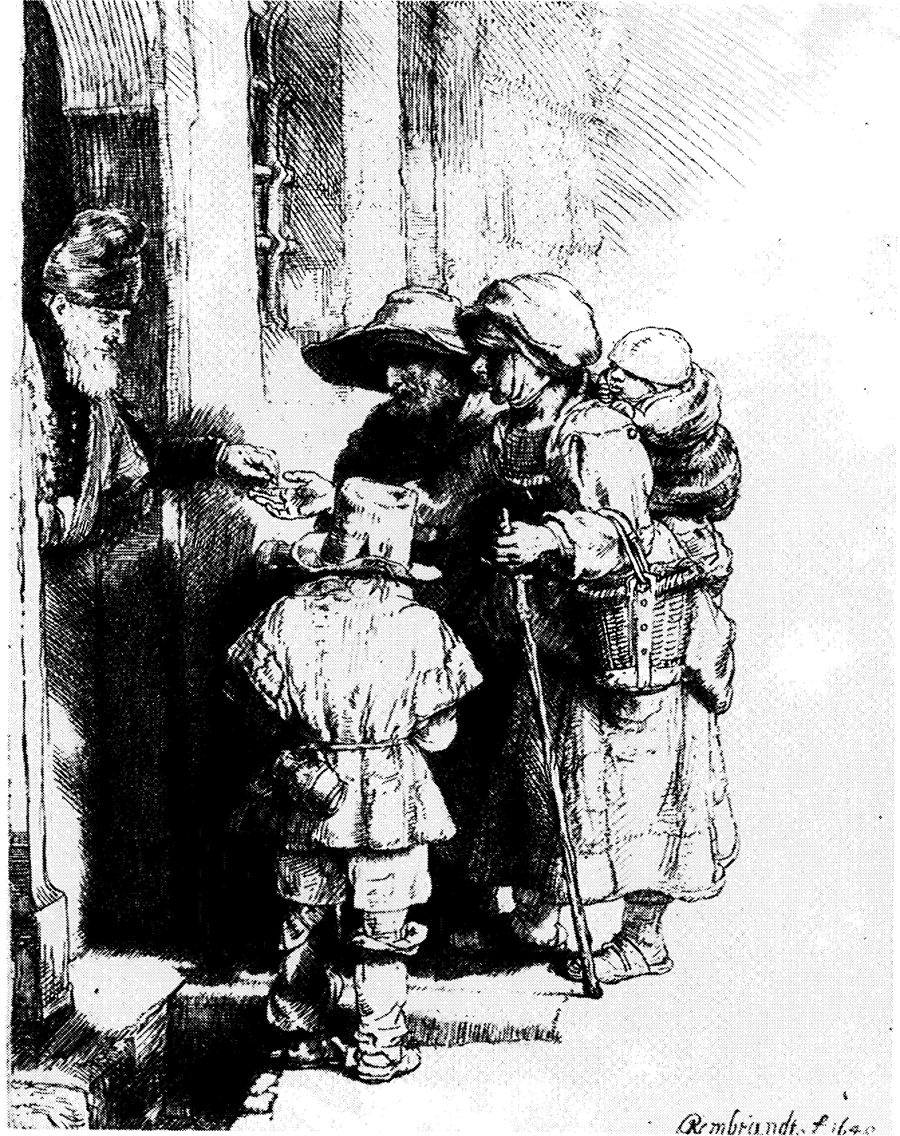
\includegraphics{include/html/images/356_1.png}

PLATE 41. Rembrandt Harmensz van Rijn. \emph{The Beggars}. Courtesy Foto
Marburg/Art Resource, New York.

\protect\hypertarget{20_ILLUSTRATIONS_FOLLOW_PAGE.xhtmlux5cux23id_37}{}{}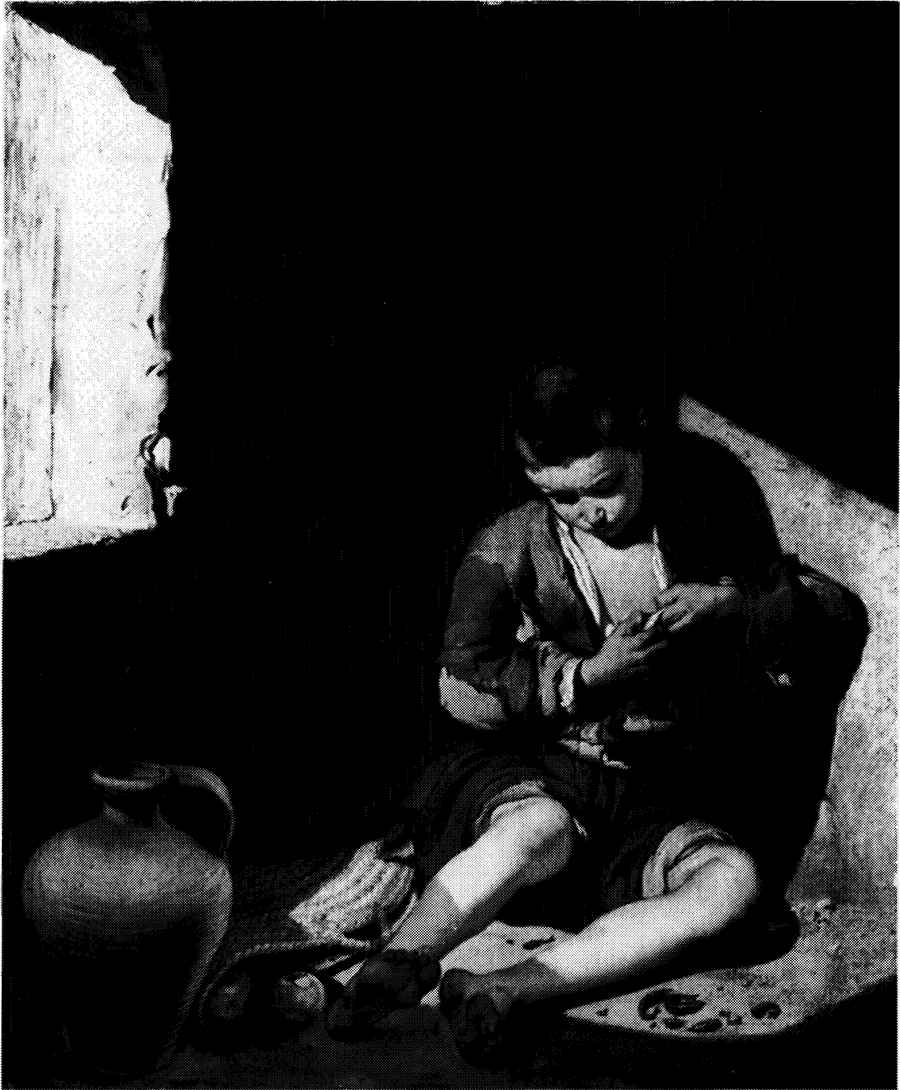
\includegraphics{include/html/images/357_1.png}

PLATE 42. Murillo, Bartolomé. \emph{Beggar Boy}. Louvre, Paris. Cliché
des Musées Nationaux-Paris.

\protect\hypertarget{20_ILLUSTRATIONS_FOLLOW_PAGE.xhtmlux5cux23id_38}{}{}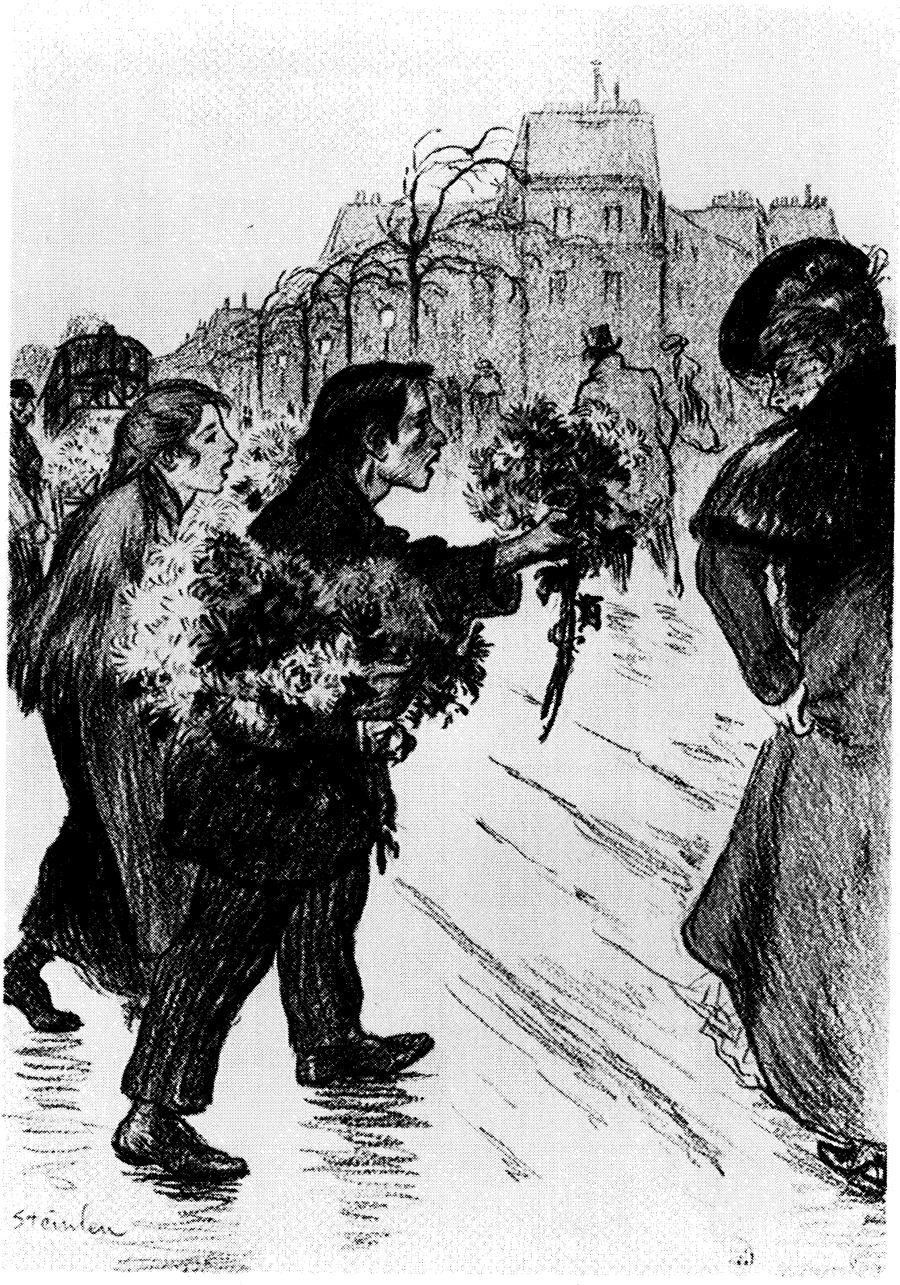
\includegraphics{include/html/images/358_1.png}

PLATE 43. Steinlen, Theophile. \emph{Flower Sellers on the Boulevard}.
Musée de la Ville de Paris, Musée Carnavalet, Paris.

\protect\hypertarget{20_ILLUSTRATIONS_FOLLOW_PAGE.xhtmlux5cux23id_39}{}{}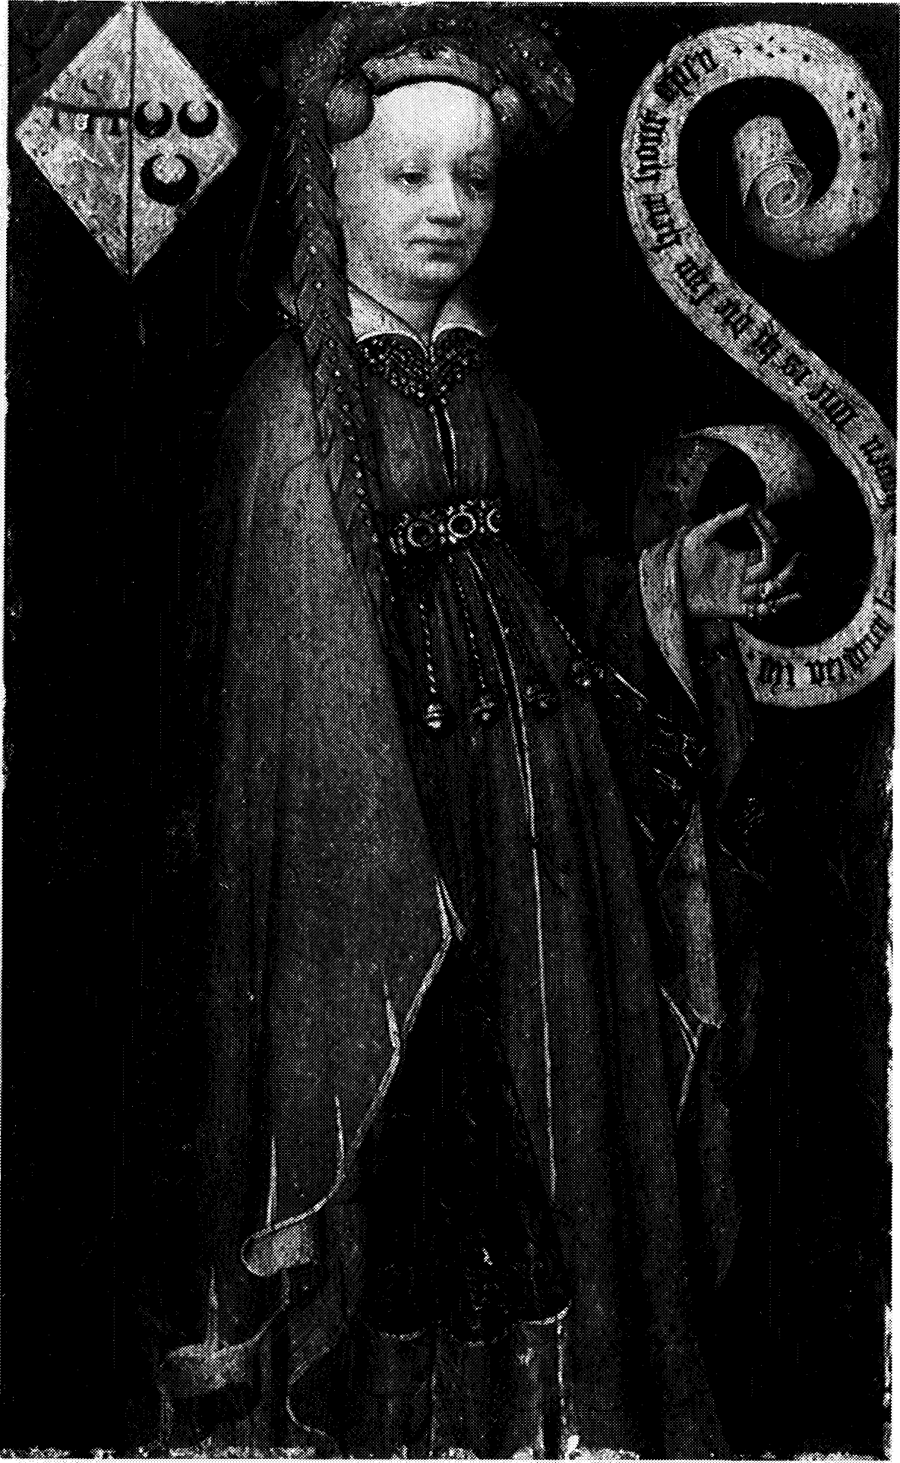
\includegraphics{include/html/images/359_1.png}

PLATE 44. Northern Netherlands School: \emph{Lysbeth van Durenvoode}.
Rijksmuseum, Amsterdam.

\protect\hypertarget{20_ILLUSTRATIONS_FOLLOW_PAGE.xhtmlux5cux23id_40}{}{}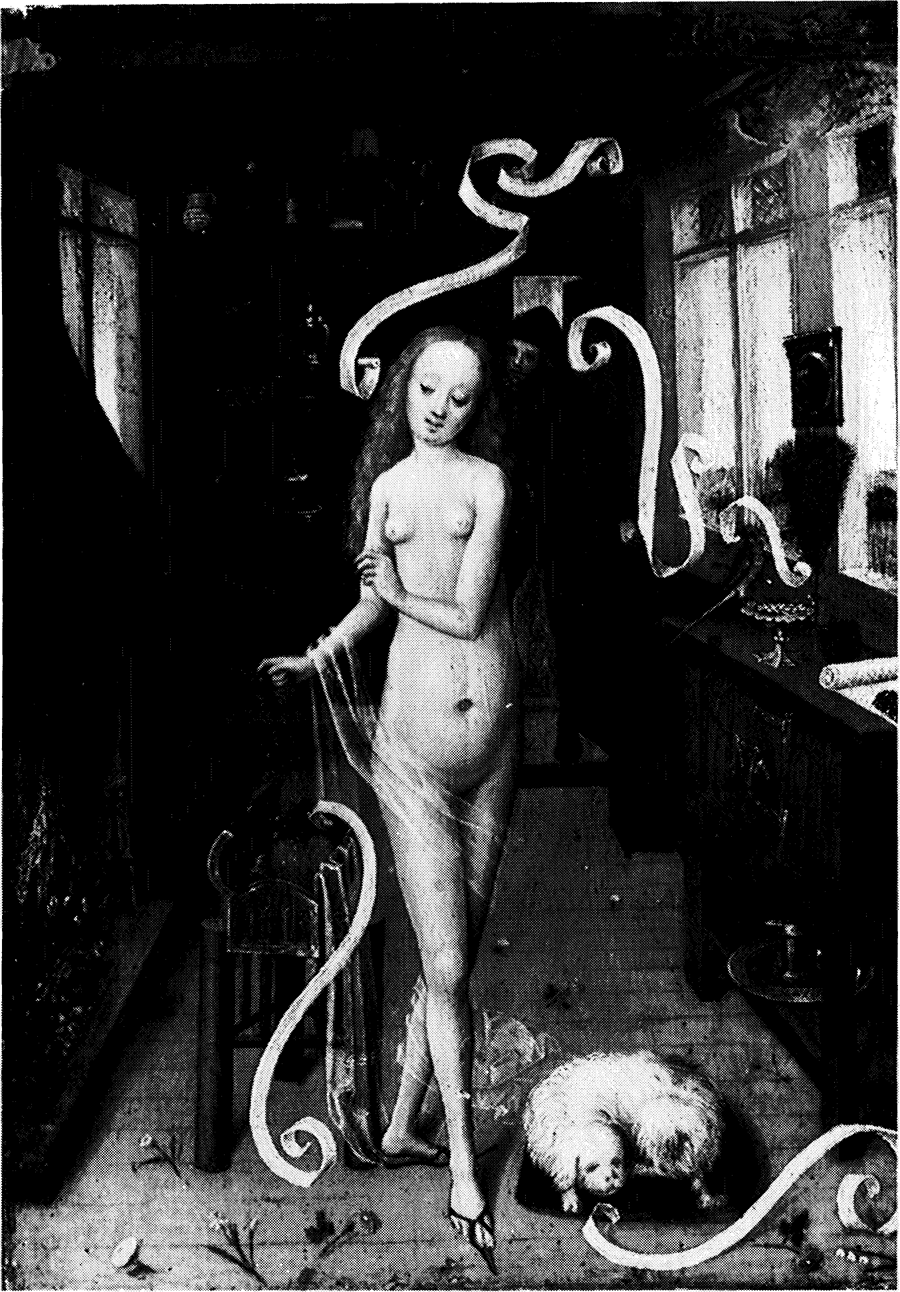
\includegraphics{include/html/images/360_1.png}

PLATE 45. Master of the Bonner Diptych: \emph{Love Magic}. Museum der
Bildenden Künste, Leipzig.

\protect\hypertarget{20_ILLUSTRATIONS_FOLLOW_PAGE.xhtmlux5cux23page_299}{}{}Of
the many works from the hands of the great and not so great artists only
a fraction of a rather special kind have been preserved. These are
primarily tomb monuments, altarpieces, portraits, and miniatures. With
the exception of portraits, only very little survives of secular
painting. Of the ornamental arts and crafts, we have a number of
specific categories: church utensils, clerical vestments, some
furniture. How much would our insight into the character of the art of
the fifteenth century be improved if we could place the bathing scenes
of Jan van Eyck or Rogier van der Weyden or the hunting scenes side by
side with the many pietàs and madonnas. We are hardly able to form any
understanding of the entire field of the applied arts. To do so, we
would have to see the ecclesiastical paraments and the stately robes of
the court, bedecked with precious stones and bells, all together. We
would have to be able to see the splendidly decorated ships of which the
miniatures convey only a highly deficient, mechanical notion. There are
only a few things whose beauty aroused so much enthusiasm in Froissart
as that of
ships.\textsuperscript{\protect\hypertarget{20_ILLUSTRATIONS_FOLLOW_PAGE.xhtmlux5cux23id_453}{\protect\hyperlink{23_NOTES.xhtmlux5cux23page_432}{10}}}
The banners, richly decorated with coats of arms,
\protect\hypertarget{20_ILLUSTRATIONS_FOLLOW_PAGE.xhtmlux5cux23page_300}{}{}fluttering
from the tops of the mast, were sometimes so long that they touched the
water. In the paintings of ships by Peter Breughel these unusually long
and broad streamers can still be seen
(\protect\hyperlink{20_ILLUSTRATIONS_FOLLOW_PAGE.xhtmlux5cux23id_13}{plate
12}). The ship of Philip the Bold, on which Melchior Broederlam worked
in 1387 at Sluis, was covered with blue and gold; large coats of arms
graced the pavilion of the aftercastle. The sails were strewn with
marguerites, the initials of the ducal couple and their slogan, ``Il me
tarde.'' Noblemen vied with one another to see whose ship was most
expensively decorated for the expedition to England. Painters are well
off, says
Froissart,\textsuperscript{\protect\hypertarget{20_ILLUSTRATIONS_FOLLOW_PAGE.xhtmlux5cux23id_451}{\protect\hyperlink{23_NOTES.xhtmlux5cux23id_452}{11}}}
they are able to demand any price, and there are never enough of them.
He claims that many ships had the masts covered with gold leaf. Guy de
la Trémoïlle, in particular, spared no expense: He spent more than two
thousand pounds for gilding. ``L'on ne se povoit de chose adviser pour
luy jolyer, ne deviser, que le seigneur de la Trimouille ne le feist
faire en ses nefs. Et tout ce paioient les povres gens parmy France
.~.~. ``
\protect\hypertarget{20_ILLUSTRATIONS_FOLLOW_PAGE.xhtmlux5cux23id_2661}{\protect\hyperlink{23_NOTES.xhtmlux5cux23id_2662}{*\textsuperscript{4}}}

This taste for splendid extravagance would undoubtedly catch our
attention forcefully if we could see the lost secular decorative arts.
The surviving works of art most decidedly do share that tendency towards
extravagance, but since we value this quality in art least, we pay less
attention to it. We only seek to enjoy the profound beauty of any given
work. Everything that is mere splendor and pomp has lost its attraction
for us. For contemporaries, however, this very pomp and splendor was of
tremendous importance.

French-Burgundian culture of the waning Middle Ages counts among those
cultures in which beauty is replaced by splendor. Late medieval art
reflects the spirit of the late Middle Ages faithfully, a spirit that
had run its course. What we had posited as one of the most important
characteristics of late medieval thought, the depiction of everything
that could be thought down to the smallest detail, the oversaturation of
the mind with an endless system of formal representation, this, too,
constitutes the essence of the art of that time. Art, too, tries to
leave nothing unformed, unpresented, or undecorated. The flamboyant
Gothic is like an endless organ postlude; it breaks down all forms by
this self-analyzing
\protect\hypertarget{20_ILLUSTRATIONS_FOLLOW_PAGE.xhtmlux5cux23page_301}{}{}process;
every detail finds its continuous elaboration, each line its
counterline. It is an unrestrainedly wild overgrowth of the idea by the
form; ornate detail attacks every surface and line. That \emph{horror
vacui}, which may perhaps be identified as a characteristic of end
periods of intellectual development, dominates in this art.

This all means that the boundaries between splendor and beauty become
less distinct. Embellishment and ornamentation no longer serve the
glorification of the naturally beautiful, but rather overgrow and thus
threaten to choke it. The farther the departure from purely pictorial
art, the more unrestrained the wild overgrowth of formal ornamentation
covering content. There is little opportunity for sculpture to engage in
this wild growth of forms as long as it creates freestanding figures:
the statues of the Moses Fountain and the
``plourants''\textsuperscript{\protect\hypertarget{20_ILLUSTRATIONS_FOLLOW_PAGE.xhtmlux5cux23id_449}{\protect\hyperlink{23_NOTES.xhtmlux5cux23id_450}{12}}}
of the tombstones compete, in their strict, simple, naturalness, with
Donatello. But as soon as the task of the art of sculpture is of a
decorative nature or falls into the realm of painting and, bound by the
reduced dimensions of the relief, reproduces entire scenes, sculpture,
too, overindulges in restless, overloaded displays. Those who see the
carvings by Jacques de Baerze at the tabernacle in Dijon next to the
paintings of Broederlam will notice the disharmony between them
(\protect\hyperlink{20_ILLUSTRATIONS_FOLLOW_PAGE.xhtmlux5cux23id_14}{plate
13}). In painting, wherever it is purely representational, simplicity
and quietude dominate; carving, by its very nature decorative, treats
the shaping of figures ornamentally, and one perceives the phenomenon of
forms crowding each other out as something that supplants the quietude
of the painted object. The difference between painting and tapestries is
of the same kind. The art of weaving, even in cases where it assumes a
task of a purely representational nature, by virtue of its set
technique, stands closer to ornamentation and is unable to extricate
itself from the exaggerated need for embellishment. Tapestries are
overcrowded with figures and colors and remain apparently archaic in
form.\textsuperscript{\protect\hypertarget{20_ILLUSTRATIONS_FOLLOW_PAGE.xhtmlux5cux23id_447}{\protect\hyperlink{23_NOTES.xhtmlux5cux23id_448}{13}}}
Departing still further from the pure fine arts, we encounter clothing.
Clothing, too, belongs undeniably to art, but it is part of its very
purpose that allure and ostentation predominate over beauty itself.
Moreover, personal vanity pulls the art of clothing into the sphere of
passion and sensuousness where the qualities that comprise the essence
of high art, balance and harmony, come second.

An extravagance like that found in the style of dress between 1350 and
1480 has not been experienced in later ages, at least not
\protect\hypertarget{20_ILLUSTRATIONS_FOLLOW_PAGE.xhtmlux5cux23page_302}{}{}in
such a general and sustained way. Certainly there have been extravagant
fashions in later times, such as the dress of the mercenaries around
1520 and aristocratic French costume in 1660, but the unrestrained
exaggeration and overprofusion so characteristic of French-Burgundian
dress for a century has no parallel. In their dress we are privileged to
observe what the sense of beauty of that age, left to its own
undisturbed impulses, would accomplish. A court costume is overburdened
with hundreds of precious stones and all its proportions are exaggerated
to a ridiculous degree; the headdress of women assumes the sugarloaf
form of the hennin; natural hair is hidden or removed at the temples and
from the area of the forehead at the hairline, so that the curiously
vaulted foreheads that were considered beautiful were prominently
displayed. The décolletage began abruptly. Male garments, however,
displayed still more numerous extravagances; most striking of all, the
elongated toes of the shoes, the \emph{poulaines}, which the knights at
Nicopolis\textsuperscript{\protect\hypertarget{20_ILLUSTRATIONS_FOLLOW_PAGE.xhtmlux5cux23id_445}{\protect\hyperlink{23_NOTES.xhtmlux5cux23id_446}{14}}}
had to cut off in order to be able to flee, the narrow waists, the
balloon-like puffed-up sleeves that rose at the shoulders, the
houpelandes dangling to the feet, and the short jackets that barely
covered the hips, the tall caps or hats narrowing at the tips or shaped
like a cylinder, the bonnets wondrously draped around the head
reminiscent of a cock's comb or a flickering flame. The more festive the
more extravagant, since all this beauty was equated with splendor,
stateliness,
\emph{estat}.\textsuperscript{\protect\hypertarget{20_ILLUSTRATIONS_FOLLOW_PAGE.xhtmlux5cux23id_443}{\protect\hyperlink{23_NOTES.xhtmlux5cux23id_444}{15}}}
The mourning dress that Philip the Good wears after the murder of his
father while receiving the King of England is so long that it trails
from the tall horse he is riding all the way to the
ground.\textsuperscript{\protect\hypertarget{20_ILLUSTRATIONS_FOLLOW_PAGE.xhtmlux5cux23id_441}{\protect\hyperlink{23_NOTES.xhtmlux5cux23id_442}{16}}}

All this wasteful splendor reaches its climax in the festivities of the
court. Everyone remembers the descriptions of the Burgundian court
festivities, such as the banquet at Lille in 1454, where the guests took
their vows to participate in the crusade against the Turks while the
pheasants were being served, or the wedding feast of Charles the Bold
and Margaret of York at Bruges in
1468.\textsuperscript{\protect\hypertarget{20_ILLUSTRATIONS_FOLLOW_PAGE.xhtmlux5cux23id_439}{\protect\hyperlink{23_NOTES.xhtmlux5cux23id_440}{17}}}
We cannot imagine a greater distance than that which exists between the
consecrated atmosphere of the Ghent and Louvain altars and these
expressions of barbaric princely ostentation. The descriptions of all
those \emph{estremets} with pastry from within which musicians
performed, the overly ornate ships and castles, the monkeys, whales,
giants, and dwarfs, and all the worn allegory belonging to them force us
to see them as unusually insipid performances.

\protect\hypertarget{20_ILLUSTRATIONS_FOLLOW_PAGE.xhtmlux5cux23page_303}{}{}However,
isn't the distance we perceive between the two extremes of church art
and the art of the court festivities easily exaggerated in more than one
respect? First of all, we have to be clear about the function that the
festivity served in society. It still had the purpose that it had among
primitive peoples; that is, to be the sovereign expression of the
culture, to be the form in which the highest joy of life was expressed
by the community, and to express the sense of that community. During
times of great social renewal, such as at the time of the French
Revolution, festivities sometimes regain that important social and
aesthetic function.

Modern man is in a position to seek individually the confirmation of his
view of life and the purest enjoyment of his \emph{joie de vivre} during
any moment of leisure in self-chosen relaxations. But an age in which
the spiritual luxuries are still poorly distributed and less accessible
requires for the purpose of renewal a communal act: the festival. The
greater the contrast with the misery of daily life, the more
indispensable the festival and the stronger the means required to bestow
splendor on life by virtue of the ecstasy of beauty and enjoyment that
lights up the darkness of reality. The fifteenth century was an age of
great emotional depression and thorough pessimism. We have already
mentioned earlier the permanent pressure from injustice and violence,
hell and damnation, pestilence, fire and hunger, Satan and the witches,
under which the century lived. Mankind in its wretchedness needed more
than the daily repeated promise of heavenly bliss and God's watchful
care and benevolence: from time to time a glorious, solemn, and communal
affirmation of the beauty of life was required. The enjoyment of life in
its primary forms---play, love, drink, dance, and song---does not
suffice. Life has to be ennobled through beauty, to be stylized in a
social expression of the joy of life. For the individual, relief through
the reading of books, listening to music, seeing art, or enjoying nature
was still out of reach; books were too expensive, nature too dangerous,
and art was no more than a small part of the festival.

The folk festival had only song and dance for its original sources of
beauty. For the beauty of color and form folk festivals based themselves
on church festivals, which had both in abundance, and usually took place
immediately after a church festival. The separation of the urban
festival from the church form, and its establishment of a decor of its
own, took place throughout the entire
fif\protect\hypertarget{20_ILLUSTRATIONS_FOLLOW_PAGE.xhtmlux5cux23page_304}{}{}teenth
century through the labor of the rhetoricians. Prior to this time, the
princely courts had been in a position both to arrange a purely secular
festival with an attendant display of art and to bestow on the festival
a splendor of its own. But display and splendor are not sufficient for
festivals; nothing is as indispensable for them as style.

The church festival possessed style because of its liturgy. In a
beautiful communal social gesture the church festivals always managed to
give moving expression to a lofty idea. The sacred dignity and noble
stateliness of the ceremonies were not destroyed even by the most
extreme overgrowth of festive details, which bordered on the burlesque.
But from where were court festivals to obtain style? On which conception
was it to be based?---The answer could be none other than the chivalric
ideal, because the entire life of the court was based on it. Was the
chivalric ideal tied to a style, to a liturgy, so to speak? Indeed;
everything related to the act of bestowing knighthood, the rules of
orders, tournaments, \emph{préséance, hommage}, and service, the entire
game of the kings at arms, heralds, coats of arms, constituted the
style. To the degree the court festival was based on those elements, it
most decidedly possessed in the eyes of contemporaries a greatly
elevated style. Strong sensitivity to the stylish festive air of the
ceremonial procedure frequently comes naturally to modern man,
independent of all the awe with which all matters aristocratic or
monarchic are seen. How much more so it must have been for those who
were still captivated by the delusion of that chivalric ideal whenever
they encountered the pompous display of costumes with their long trains
and glittering colors!

But court festivals aspired to more. They wanted to present the dream of
the heroic life in its extreme form. This is where the style failed. The
entire apparatus of knightly fancy and splendor was no longer filled
with real life. Everything had become much too literary, a sickly
renaissance, an empty convention. The inner decay of the form of life
remained hidden under the overload of glamour and etiquette. The
chivalric idea of the fifteenth century revels in a romanticism that is
hollow and worn throughout. And that was the source from which the court
festival was supposed to derive the inspiration for its performances and
presentations. How could it create a style from such a styleless,
undisciplined, and stale literature as that of chivalric romanticism in
its decay?

\protect\hypertarget{20_ILLUSTRATIONS_FOLLOW_PAGE.xhtmlux5cux23page_305}{}{}The
aesthetic value of the \emph{entremets} should be seen in this light:
They were applied literature. Actually, this was the only way this
literature could be made bearable, since in the \emph{entremets} the
fleeting, superficial shapes of all the colorful literary dream figures
had to make room for the necessity of the material representation.

The heavy barbarian seriousness evident in all this fits well into the
Burgundian court, which seemed to have lost the lighter and more
harmonious French spirit through its contact with the North. All the
tremendous display is taken solemnly and seriously. The great festivity
of the duke at Lille was both the end and the climax of a number of
banquets given by the court nobility in competition with each other. All
this had started quite simply and with little expense; the number of
guests and the luxury of the menus and \emph{entremets} were gradually
increased. By being offered a wreath by his host, a guest was designated
to take his turn as successor; in this manner the knights were followed
by the great lords and the great lords by the princes, all this with
steadily increasing expense and stateliness, until it was finally the
turn of the duke himself. But Philip intended to hold more than a
splendid feast; he intended to collect vows for the crusade against the
Turks for the reconquest of Constantinople, which had fallen a year
earlier. This was the officially proclaimed goal of the duke's life. To
prepare for the feast, he appointed a commission with the knight of the
Fleece, Jean de Lannoy, as its leader. Olivier de la Marche, too, was a
member. Whenever he comes to this issue in his memoirs he becomes very
solemn: ``Pour ce que grandes et honnorables oeuvres désirent loingtaine
renomée et perpétuelle
mémoire.''\protect\hypertarget{20_ILLUSTRATIONS_FOLLOW_PAGE.xhtmlux5cux23id_2663}{\protect\hyperlink{23_NOTES.xhtmlux5cux23id_2664}{*\textsuperscript{5}}}
These are the words with which he begins to reminisce about those great
events.\textsuperscript{\protect\hypertarget{20_ILLUSTRATIONS_FOLLOW_PAGE.xhtmlux5cux23id_437}{\protect\hyperlink{23_NOTES.xhtmlux5cux23id_438}{18}}}
The first councillors, who were closest to the duke, regularly attended
the deliberations: even Chancellor Rolin and Antoine de Croy, the First
Chamberlain, were consulted before agreement was reached where ``les
cérémonies et les mistères'' should be held.

All these beautiful events have been described so often that there is no
need to do so here. Some had even crossed the channel to witness the
spectacle. Joining the guests were innumerable noble onlookers, the
majority of whom were masked. First the guests took a stroll to admire
the splendid stationary displays; then came
\protect\hypertarget{20_ILLUSTRATIONS_FOLLOW_PAGE.xhtmlux5cux23page_306}{}{}the
performances with living persons and \emph{tableaux vivants}. Olivier
himself played the leading role of Sainte Eglise when she entered during
the most important scene inside a tower placed on the back of an
elephant led by a giant Turk. The tables were given the most marvelous
decorations: a manned
carrack\textsuperscript{\protect\hypertarget{20_ILLUSTRATIONS_FOLLOW_PAGE.xhtmlux5cux23id_435}{\protect\hyperlink{23_NOTES.xhtmlux5cux23id_436}{19}}}
with full sails, a meadow with trees, a spring, rocks, and a picture of
St. Andreas, Lusignan Castle with the fairy Melusine, a windmill and a
bird-shooting scene, a forest with moving wild animals, and, finally,
the church with an organ and singers that, alternating with the
twenty-eight-man orchestra that was sitting in a pie, offered musical
performances.

What matters here is the degree of taste or tastelessness that is found
in all this. The subject matter itself is nothing but a loose mixture of
mythological, allegorical, and moralizing images, but what about the
execution? There is no doubt that the effect was largely sought through
extravagance. The Tower of Gorkum that served as ostentatious table
decoration during a 1468 wedding celebration was forty-six feet
tall.\textsuperscript{\protect\hypertarget{20_ILLUSTRATIONS_FOLLOW_PAGE.xhtmlux5cux23id_433}{\protect\hyperlink{23_NOTES.xhtmlux5cux23id_434}{20}}}
La Marche reports about a whale fashioned for the same occasion: ``Et
certes ce fut un moult bel entremectz, car il y avoit dedans plus de
quarante
personnes.''\textsuperscript{\protect\hypertarget{20_ILLUSTRATIONS_FOLLOW_PAGE.xhtmlux5cux23id_431}{\protect\hyperlink{23_NOTES.xhtmlux5cux23id_432}{21}}}\protect\hypertarget{20_ILLUSTRATIONS_FOLLOW_PAGE.xhtmlux5cux23id_2665}{\protect\hyperlink{23_NOTES.xhtmlux5cux23id_2666}{*\textsuperscript{6}}}
As to the miracles of mechanical gadgetry, such as the living birds that
fly out of the mouth of the dragon with whom Hercules does battle and
other such astonishing contraptions, it is difficult to associate them
with any notion of art. The comic element is only poorly represented in
them. From inside the Gorkum tower, wild boars play trumpets, goats
perform a motet, wolves play the flute, four large asses perform as
singers---and do so before Charles the Bold, who was a connoisseur of
music of some stature.

I do not wish to cast doubt that, in spite of everything, there were
found among all the displays of the festival, particularly among the
sculptural pieces, a good many genuine works of art alongside the
predominantly silly ostentation. We should remember that the people who
delighted in this gargantuan splendor and wasted serious thought on it
were the same people who commissioned the works of Jan van Eyck and
Rogier van der Weyden. The duke himself was their patron, as was Rolin,
the donor of the altars of Beaune
(\protect\hyperlink{20_ILLUSTRATIONS_FOLLOW_PAGE.xhtmlux5cux23id_2298}{plate
14}) and Autun
(\protect\hyperlink{20_ILLUSTRATIONS_FOLLOW_PAGE.xhtmlux5cux23id_15}{plates
15},
\protect\hyperlink{20_ILLUSTRATIONS_FOLLOW_PAGE.xhtmlux5cux23id_16}{16}),
and Jean
\protect\hypertarget{20_ILLUSTRATIONS_FOLLOW_PAGE.xhtmlux5cux23page_307}{}{}Chevrot,
who was the patron of Rogier's \emph{Seven Sacraments}
(\protect\hyperlink{20_ILLUSTRATIONS_FOLLOW_PAGE.xhtmlux5cux23id_17}{plate
17}), and many others, such as Lannoy. It is even more significant that
the creators of these and similar ostentations were these very same
painters. Though it happens that we have no definite information about
Jan van Eyck or Rogier, we do know it to be a fact that others, Colard
Marmion, Simon Marmion, and Jacques Daret, for example, often had a hand
in such festivals. For the festival in 1468, the date of which was
unexpectedly moved up, the entire guild of painters was mobilized to
assure completion; in great haste journeymen from Ghent, Brussels,
Louvain, Thirlemont, Bergen, Quesnoy, Valenciennes, Douai, Cambrai,
Arras, Lille, Ypres, Courtray, and Oudenarde were dispatched to
Bruges.\textsuperscript{\protect\hypertarget{20_ILLUSTRATIONS_FOLLOW_PAGE.xhtmlux5cux23id_429}{\protect\hyperlink{23_NOTES.xhtmlux5cux23id_430}{22}}}
What was produced by their hands cannot have been completely ugly. One
would readily exchange many a mediocre altarpiece for the thirty fully
equipped ships, complete with the coats of arms of the ducal lords, of
the banquet of 1468, the sixty women in different regional
costumes\textsuperscript{\protect\hypertarget{20_ILLUSTRATIONS_FOLLOW_PAGE.xhtmlux5cux23id_427}{\protect\hyperlink{23_NOTES.xhtmlux5cux23id_428}{23}}}
holding fruit baskets and bird cages, and the windmills and bird
catchers.

Even at the risk of sacrilege, it is tempting to go one step further and
assert that on occasion we have to keep in mind this lost art of table
decoration, now completely vanished, in order to better understand Claus
Sluter\textsuperscript{\protect\hypertarget{20_ILLUSTRATIONS_FOLLOW_PAGE.xhtmlux5cux23id_425}{\protect\hyperlink{23_NOTES.xhtmlux5cux23id_426}{24}}}
and others like him.

Among the other arts, that of funeral sculpture served a clearly
practical function. The task facing the sculptors charged with creating
the tomb monuments for the Burgundian dukes was not one of imaginative
beauty, but was rather concerned with glorifying princely grandeur.
Their task was much more strictly limited and more precisely prescribed
than that of the painters, who in commissioned works were allowed to
give much freer reign to their creative urges and who could paint
whatever they wanted when not working on a commission. The sculptor of
that age probably did little work outside of his commissions and the
motifs of his work were limited in number and tied to a strong
tradition. Sculptors were then much more tightly dependent on the dukes
than the painters. The two great Dutch artists who were enticed out of
their country by the magnet of French artistic life were totally
monopolized by the duke of Burgundy. Sluter lived in a house in Dijon
assigned and furnished for him by the
duke.\textsuperscript{\protect\hypertarget{20_ILLUSTRATIONS_FOLLOW_PAGE.xhtmlux5cux23id_423}{\protect\hyperlink{23_NOTES.xhtmlux5cux23id_424}{25}}}
He lived there like a great lord, but at the same time like an employee
of the court. The court rank ``varlet de chambre de monsegneur le
duc\protect\hypertarget{20_ILLUSTRATIONS_FOLLOW_PAGE.xhtmlux5cux23page_308}{}{}de
Bourgogne,''\protect\hypertarget{20_ILLUSTRATIONS_FOLLOW_PAGE.xhtmlux5cux23id_2667}{\protect\hyperlink{23_NOTES.xhtmlux5cux23id_2668}{*\textsuperscript{7}}}
which Sluter shared with his cousin Claes van de Werve and Jan van Eyck,
had an authoritative meaning for the sculptors. Claes van de Werve, who
continued Sluter's work, became one of the tragic victims of art in the
service of the court: kept in Dijon year in and out in order to complete
the tomb monument of John the Fearless
(\protect\hyperlink{20_ILLUSTRATIONS_FOLLOW_PAGE.xhtmlux5cux23id_18}{plate
18}), a task for which there were never funds available, his splendidly
promising career wasted away in futile waiting and he died having never
been able to finish his task.

This relationship of servitude, however, runs contrary to the fact that
it is in the nature of the art of sculpture always to approach a certain
peak of simplicity and freedom, primarily because of the limited nature
of its means, its material, and its subject matter. We call this peak of
simplicity and freedom classicism. It is reached as soon as one of the
great masters, even be it only one, regardless of time and place, guides
the chisel. No matter what the task the age intends to force upon the
art of sculpture, the human figure and its clothing allow for only a few
variations in their depiction in wood and stone. The differences between
the Roman portrait sculpture of the Imperial period, Goujon and Colombe
in the sixteenth century, and Houdon and Pajou in the eighteenth are
much smaller than in any other field of art.

The art of Sluter, and those like him, shares in the eternal nature of
the art of sculpture. And yet .~.~. we don't perceive Sluter's works as
they really were and were intended to be. As soon as one visualizes the
Moses Fountain, just in the manner it delighted its contemporaries at
the time when the papal legate (1418) granted absolution to anyone who
visited it with pious intentions---one realizes why we dared to mention
Sluter's art and that of the \emph{entre-mets} in one breath.

The Moses Fountain is known only as a fragment
(\protect\hyperlink{20_ILLUSTRATIONS_FOLLOW_PAGE.xhtmlux5cux23id_19}{plate
20}). The first duke of Burgundy wished to see the fountain, surmounted
by an image of the Mount of Calvary, put into the yard of the
Carthusians in his beloved Champmol. The main part of the work is
comprised of the figure of the crucified Christ with Mary, John, and the
Magdalen placed at the foot of the cross. The work had already vanished,
for the most part, prior to the Revolution, which so irretrievably
disfigured the Champmol. Below the central part,
\protect\hypertarget{20_ILLUSTRATIONS_FOLLOW_PAGE.xhtmlux5cux23page_309}{}{}and
surrounding the base that is held up around the edge by angels, stand
the six figures from the Old Testament who prophesied the death of the
Messiah: Moses, David, Isaiah, Jeremiah, Daniel, and Zachariah, each
with an attached banderole on which the prophetic texts can be read. The
entire depiction has to the highest degree the character of a
performance. This is not so much because of the fact that the
\emph{tableaux vivants} or ``personnages,'' which during processions and
banquets usually had figures with such banderoles attached to them, or
that the Messiah prophecies from the Old Testament were the most
important subjects of such representations, as because of the fact that
this depiction has an unusually strong verbal effect about it. The words
of the inscriptions have an emphasized place of importance. We only
reach a full understanding of the work if we completely absorb the
sacred import of those
texts.\textsuperscript{\protect\hypertarget{20_ILLUSTRATIONS_FOLLOW_PAGE.xhtmlux5cux23id_421}{\protect\hyperlink{23_NOTES.xhtmlux5cux23id_422}{26}}}
``Immolabit enum universa multitudo filiorum Israel ad vesperam,'' reads
Moses's dictum. ``Foderunt manus meas et pedes meos, dinumeraverunt
omnia ossa mea,'' is the citation from the Psalms of David. ``Sicut ovis
ad occisionem ducetur et quasi agnus coram tondente se obmutescet et non
aperiet os suum,'' from Isaiah. ``O vos omnes qui transitis per viam,
attendite et videte si est dolor sicut dolor meus,'' Jeremiah. ``Post
hebdomades sexaginta duas occidetur Christus,'' Daniel. ``Appenderunt
mercedem meam triginta argenteos,'' Zachariah. So reads the lament,
rising in six voices around the base of the cross. This is the essential
feature of the work. And the connection between the figures and the text
is stressed with such emphasis, there is something so compelling in the
gesture of one figure and the face of another, that the entire group is
almost in danger of losing the ataraxia that is the privilege of all
great sculpture. The viewer is addressed almost too directly. Sluter
knew, as few artists have, how to express the sanctity of his subject
matter. But, from the point of view of pure art, this weight of sanctity
constitutes something overdone. Compared with Michelangelo's tomb
figures, Sluter's prophets are too expressive, too personal. We would
perhaps consider this criticism to be doubly meritorious if more than
only the head and torso of the main figure of Christ in his rigid
majesty had been preserved. All we can see is how the angels, those
wondrously poetic angels who in their naive grace are so infinitely more
angelic than the angels of Van Eyck, direct the devotion of the prophets
to the scene above them.

The strongly representative character of the Calvary of
Champ\protect\hypertarget{20_ILLUSTRATIONS_FOLLOW_PAGE.xhtmlux5cux23page_310}{}{}mol
is based, however, on something other than its purely sculptural
qualities; that is, on the splendor in which the entire work was cast.
It should be imagined as if it were painted in polychrome by Jean
Maelweel and gilded by Hermann of
Cologne.\textsuperscript{\protect\hypertarget{20_ILLUSTRATIONS_FOLLOW_PAGE.xhtmlux5cux23id_419}{\protect\hyperlink{23_NOTES.xhtmlux5cux23id_420}{27}}}
Not a single colorful or dramatic effect had been left out. The prophets
in their golden coats were standing on green pedestals; Moses and
Zachariah in red robes, their coats lined in blue; David entirely in
blue with golden stars; Jeremiah in dark blue; Jessiah, the saddest of
them all, in brocade. Golden suns and initials filled the empty areas.
Add to all this the coats of arms! The proud coats of arms of the ducal
region gleamed not only on the shaft of the base below the prophets, but
even on the crosspiece of the great, entirely gilded cross---on its
extensions shaped like capitals had been placed the coats of arms of
Burgundy and Flanders! This, perhaps more than the gilded copper pair of
glasses, supplied by Hannequin de Hacht for the nose of Jeremiah,
testifies to the spirit that gave rise to this grand ducal work of art.

The dependence of this work on its princely sponsors contributes to a
somewhat tragic and elevated element because of the greatness by means
of which the artist manages to evade the restrictions of his commission.
The representation of the ``Plourants'' around the sarcophagus had
become obligatory in Burgundian funeral art long
ago.\textsuperscript{\protect\hypertarget{20_ILLUSTRATIONS_FOLLOW_PAGE.xhtmlux5cux23id_417}{\protect\hyperlink{23_NOTES.xhtmlux5cux23id_418}{28}}}
Its aim was not a creative expression of pain in all its depths, but
rather only a very realistic depiction of a part of the actual
procession that had accompanied the body to the grave and with all the
dignitaries readily recognizable. How skillfully Sluter and his
assistants managed to turn this motif into a profound and dignified
depiction of grief, into a funeral march in stone!

But this may perhaps be overstating the assumption of disharmony between
sponsor and artist. It is not entirely certain that it was not Sluter
himself who found the pair of glasses on Jeremiah to be a great idea.
Taste and tastelessness were, so to speak, not separated in the minds of
that age; the genuine appreciation of art and the infatuation with pomp
and curiosities had not yet parted company. The naive imagination was
still able to enjoy without embarrassment that which was bizarre as if
it were beautiful. A collection such as that in the Green Vault in
Dresden displays the separated \emph{caput mortuum} that had once been a
whole with the princely art collections. In Hesdin Castle, which was
both a treasure house of art and a pleasure garden filled with those
mechanical
\protect\hypertarget{20_ILLUSTRATIONS_FOLLOW_PAGE.xhtmlux5cux23page_311}{}{}amusements,
\emph{engins d'esbatement}, Caxton came across a room decorated with
paintings depicting the story of Jason, the hero of the Golden Fleece.
For the sake of greater effect, lightning, thunder, snow, and rain
making implements were attached in imitation of Medea's magic
tricks.\textsuperscript{\protect\hypertarget{20_ILLUSTRATIONS_FOLLOW_PAGE.xhtmlux5cux23id_415}{\protect\hyperlink{23_NOTES.xhtmlux5cux23id_416}{29}}}

Imagination was also freely indulged in creating the performances, the
\emph{personnages}, which were placed on street corners during princely
entry processions. During the 1389 entry into Paris of Isabella of
Bavaria as wife of Charles VI, a white stag with gilded antlers and a
crown around its
neck\textsuperscript{\protect\hypertarget{20_ILLUSTRATIONS_FOLLOW_PAGE.xhtmlux5cux23id_413}{\protect\hyperlink{23_NOTES.xhtmlux5cux23id_414}{30}}}
was placed among the holy scenes. The stag rested on a \emph{lit de
justice} and moved his eyes, antlers, feet, and, to conclude, raised a
sword. During the same procession an angel ``par engins bien
faits''\protect\hypertarget{20_ILLUSTRATIONS_FOLLOW_PAGE.xhtmlux5cux23id_2669}{\protect\hyperlink{23_NOTES.xhtmlux5cux23id_2670}{*\textsuperscript{8}}}
descended from the tower of Notre Dame, entered through a gap in the
blue taffeta canopy covering the entire bridge just at the moment the
queen passed by, placed a crown on her head and disappeared in the same
way it had arrived ``comme s'il s'en fust retourné de soy mesmes au
ciel.''\textsuperscript{\protect\hypertarget{20_ILLUSTRATIONS_FOLLOW_PAGE.xhtmlux5cux23id_411}{\protect\hyperlink{23_NOTES.xhtmlux5cux23id_412}{31}}}\protect\hypertarget{20_ILLUSTRATIONS_FOLLOW_PAGE.xhtmlux5cux23id_2671}{\protect\hyperlink{23_NOTES.xhtmlux5cux23id_2672}{†\textsuperscript{9}}}
Philip the Good is presented with a similarly descending
maiden\textsuperscript{\protect\hypertarget{20_ILLUSTRATIONS_FOLLOW_PAGE.xhtmlux5cux23id_409}{\protect\hyperlink{23_NOTES.xhtmlux5cux23id_410}{32}}}
during an entry into Ghent, as is Charles VII in Reims in
1484.\textsuperscript{\protect\hypertarget{20_ILLUSTRATIONS_FOLLOW_PAGE.xhtmlux5cux23id_407}{\protect\hyperlink{23_NOTES.xhtmlux5cux23id_408}{33}}}
We are hard put to imagine anything more silly than a so-called
pantomime horse moved by a man inside, but during the fifteenth century
this was apparently not the case. In any event, Le Fèvre de Saint Remy
reports, without a trace of ridicule, about a performance by four
trumpeters and twelve noblemen ``sur chevaulx de artifice,'' ``saillans
et poursaillians tellement que belle chose estoit à
veoir.''\textsuperscript{\protect\hypertarget{20_ILLUSTRATIONS_FOLLOW_PAGE.xhtmlux5cux23id_405}{\protect\hyperlink{23_NOTES.xhtmlux5cux23id_406}{34}}}\protect\hypertarget{20_ILLUSTRATIONS_FOLLOW_PAGE.xhtmlux5cux23id_2673}{\protect\hyperlink{23_NOTES.xhtmlux5cux23id_2674}{‡\textsuperscript{10}}}

The separation of all that bizarre decoration, which has vanished
without a trace, from the individual works of art that have been
preserved, a separation that our appreciation of art demands and that
has been aided by the all destroying passage of time, hardly existed for
contemporaries. The artistic life of the Burgundian age was still
entirely determined by the forms of social life. Art served. It had
primarily a social function; this was primarily to display splendor and
to emphasize the importance of the individual, not the artist but rather
the donor. This is not contradicted by the fact
\protect\hypertarget{20_ILLUSTRATIONS_FOLLOW_PAGE.xhtmlux5cux23page_312}{}{}that
in church art, pompous splendor serves to direct pious thoughts upward
and that the donor, out of a pious impulse, puts his own figure in the
foreground. On the other hand, the art of secular painting is not always
as luxuriant and arrogant as would be suitable for bloated courtly life.
Too much is missing of the entire environment in which art existed for a
clear understanding of the manner in which art and life touched and
dissolved in each other. Moreover, our knowledge of this art itself is
much too fragmentary for that purpose. It is not court and church alone
that comprise the life of that age.

This is the reason for the special importance of the few works of art in
which something of the life outside those two spheres finds its
expression. One of these works radiates in its own peerless delight: the
portrait of the Arnolfini \emph{Marriage}
(\protect\hyperlink{20_ILLUSTRATIONS_FOLLOW_PAGE.xhtmlux5cux23id_20}{plate
21}). It represents the art of the fifteenth century in its purest form
and allows us to come closest to the enigmatic personality of the
painter Jan van Eyck. Painting the portrait did not require that he
reproduce the splendid majesty of God nor sense the haughtiness of the
nobleman: he painted his friends on the occasion of their wedding. Was
the subject of the painting really Jean Arnoulphin, as he was called in
Flanders, the merchant from Lucca? This face, which Jan van Eyck painted
twice,\textsuperscript{\protect\hypertarget{20_ILLUSTRATIONS_FOLLOW_PAGE.xhtmlux5cux23id_403}{\protect\hyperlink{23_NOTES.xhtmlux5cux23id_404}{35}}}
is not at all Italian. But the title of the painting as \emph{Hernoul le
fin avec sa femme dedens une chambre}, in the
1516\textsuperscript{\protect\hypertarget{20_ILLUSTRATIONS_FOLLOW_PAGE.xhtmlux5cux23id_401}{\protect\hyperlink{23_NOTES.xhtmlux5cux23id_402}{36}}}
inventory of paintings belonging to Margaret of Austria, provides strong
support for the assumption that he is Arnolfini. In that case, the
painting should not actually be called a ``bourgeois portrait,'' since
Arnolfini was a highly placed individual who repeatedly served as
adviser to the ducal government in important matters. Be that as it may,
the man depicted here was a friend of Jan van Eyck. This is shown by the
delicately phrased inscription above the mirror with which the painter
has signed his work: ``Johannes de Eyck fuit his, 1434.'' Jan van Eyck
was here. Just a short time ago. The deep silence of the chamber still
reverberates with the sound of his voice. The intimate tenderness and
the calm peace, which we are to meet again only in Rembrandt, are
encased in this work as if it were, so to speak, Jan's own heart. All of
a sudden, that evening during the Middle Ages is brought back to us, an
evening we know of, but so often seek in vain in literature, in history,
and in the life of faith of that age: the happy, noble, pure,
\protect\hypertarget{20_ILLUSTRATIONS_FOLLOW_PAGE.xhtmlux5cux23page_313}{}{}and
simple medieval age of folk song and church music. How far they are,
that loud laughter and unrestrained passion!

At this moment perhaps we can see in our imagination Jan van Eyck, who
stood outside the tension-filled, vibrant life of his time, a simple
man, a dreamer who went through life with his head bowed, looking inside
himself. Caution!---or this will turn out like an art-historical novel
about how the duke's ``varlet de chambre'' served his high lord
reluctantly, how his companions, full of pain, had to deny their high
art so that they could join the work of staging courtly festivities and
equipping fleets!

There is nothing in our possession that could justify any such notion.
The art of the Van Eycks', which we so admire, stood right in the middle
of the courtly life that is so repugnant to us. The little we know of
the life of those painters makes them appear to be men of the great
world. The duke of Berry is on the best of terms with his painters.
Froissart met him in intimate conversation with André Beauneveu in his
marvelous castle at Mehun sur
Yevre.\textsuperscript{\protect\hypertarget{20_ILLUSTRATIONS_FOLLOW_PAGE.xhtmlux5cux23id_399}{\protect\hyperlink{23_NOTES.xhtmlux5cux23id_400}{37}}}
The three brothers from Limburg, the great illustrators, delight the
duke at New Year with a surprise: a newly illustrated manuscript, ``un
livre contrefait'' consisting ``d'un piéce de bois blanc paincte en
semblance d'un livre, où il n'a nulz feuillets ne riens
escript.''\textsuperscript{\protect\hypertarget{20_ILLUSTRATIONS_FOLLOW_PAGE.xhtmlux5cux23id_397}{\protect\hyperlink{23_NOTES.xhtmlux5cux23id_398}{38}}}\protect\hypertarget{20_ILLUSTRATIONS_FOLLOW_PAGE.xhtmlux5cux23id_2349}{\protect\hyperlink{23_NOTES.xhtmlux5cux23id_2350}{*\textsuperscript{11}}}
There is no doubt that Jan van Eyck moved in courtly circles. The secret
diplomatic missions entrusted to him by Philip the Good required
knowledge of the world. He was regarded in his century as a literary man
who read the classics and studied geometry. His modest motto has a touch
of the bizarre: ``Als ik kan''---``As I can''---disguised in Greek
letters.

If not warned by these and similar facts, we may be easily inclined to
see the art of the Van Eycks as occupying a different place than it does
in the life of the fifteenth century. In our view, there were in that
time two spheres of life that were strictly separated. On the one side,
the culture of the court, the nobility, and the wealthy burghers:
boastful, craving honor and wealth, riotously colored, glowing with
passion; on the other side, the quiet, uniformly gray sphere of the
\emph{devotio moderna}: the serious men and the submissive wives of the
middle class who sought spiritual support
\protect\hypertarget{20_ILLUSTRATIONS_FOLLOW_PAGE.xhtmlux5cux23page_314}{}{}in
the Fraterhouses and from the Windesheimers. This is also the sphere of
Ruusbroec and of St. Colette. This is the sphere to which, according to
our sentiments, the art of the Van Eycks with its pious quiet mysticism
belongs. Yet it is more likely to be at home in the other sphere. The
modern \emph{dévotés} rejected the great art that unfolded during their
age. They resisted polyphonic music and even
organs,\textsuperscript{\protect\hypertarget{20_ILLUSTRATIONS_FOLLOW_PAGE.xhtmlux5cux23id_395}{\protect\hyperlink{23_NOTES.xhtmlux5cux23id_396}{39}}}
while the splendor-loving Burgundians Bishop David of Utrecht and
Charles the Bold himself had the foremost composers as their masters of
music, such men as Obrecht in Utrecht, Busnois for the duke, who even
took him with him to his camp near Neuss. The \emph{Ordinarius} of
Windesheim prohibited any embellished songs, and Thomas à Kempis states:
``If you cannot sing like the lark and the nightingale, sing like the
raven and the frogs in the pond. They sing as God has given them to
sing.''\textsuperscript{\protect\hypertarget{20_ILLUSTRATIONS_FOLLOW_PAGE.xhtmlux5cux23id_393}{\protect\hyperlink{23_NOTES.xhtmlux5cux23id_394}{40}}}
It is only natural that they commented less on painting, but they
desired their books to be simple and not to be
illustrated.\textsuperscript{\protect\hypertarget{20_ILLUSTRATIONS_FOLLOW_PAGE.xhtmlux5cux23id_391}{\protect\hyperlink{23_NOTES.xhtmlux5cux23id_392}{41}}}
It is very likely that they would have regarded even a work like the
\emph{Adoration of the Lamb} (plates 8, 9) as an expression of
unmitigated pride.

But was the separation of the two spheres really drawn as sharply as it
appears to us? We have already spoken of that earlier. There are
numerous points where the court circles and the circles of the strict
God-fearing men and women contact one another. St. Colette and Denis the
Carthusian have dealings with the dukes; Margaret of York, the second
wife of Charles the Bold, takes a lively interest in the ``reformed''
monasteries of Belgium. Beatrix of Ravenstein, one of the most prominent
individuals at the Burgundian court, wears the hair shirt under her
robes of state. ``Vestue de drap d'or et de royaux atournemens a luy
duisans, et feignant estre la plus mondaine des autres, livrant ascout à
toutes paroles perdues, comme maintes font, et monstrant de dehors de
pareil usages avecques les lascives et huiseuses, portoit journellement
la haire sur sa chair nue, jeunoit en pain et en eau mainte journée par
fiction couverte, et son mary absent couchoit en la paille de on lit
mainte
nuyt.''\textsuperscript{\protect\hypertarget{20_ILLUSTRATIONS_FOLLOW_PAGE.xhtmlux5cux23id_389}{\protect\hyperlink{23_NOTES.xhtmlux5cux23id_390}{42}}}\protect\hypertarget{20_ILLUSTRATIONS_FOLLOW_PAGE.xhtmlux5cux23id_2675}{\protect\hyperlink{23_NOTES.xhtmlux5cux23id_2676}{*\textsuperscript{12}}}
The act of turning inwardly, which had become the
per\protect\hypertarget{20_ILLUSTRATIONS_FOLLOW_PAGE.xhtmlux5cux23page_315}{}{}manent
mode of life for the modern devotees, is also known to the haughty, even
if only as a sporadic and faint echo of the sumptuous style of life.
When Philip the Good departed for Regensburg after the great feast at
Lille in order to negotiate with the emperor, several noblemen and women
of the court joined the order ``qui menèrent moult belle et saincte
vie.''\textsuperscript{\protect\hypertarget{20_ILLUSTRATIONS_FOLLOW_PAGE.xhtmlux5cux23id_387}{\protect\hyperlink{23_NOTES.xhtmlux5cux23id_388}{43}}}\protect\hypertarget{20_ILLUSTRATIONS_FOLLOW_PAGE.xhtmlux5cux23id_2677}{\protect\hyperlink{23_NOTES.xhtmlux5cux23id_2678}{*\textsuperscript{13}}}---The
chroniclers who describe with such broad detail all the pomp and
stateliness cannot help but repeat time and again a turning away from
``pompes et
beubans.''\protect\hypertarget{20_ILLUSTRATIONS_FOLLOW_PAGE.xhtmlux5cux23id_2680}{\protect\hyperlink{23_NOTES.xhtmlux5cux23id_2679}{t\textsuperscript{14}}}
Even Olivier de la Marche ponders after the feast at Lille about ``les
oultraigeux excés et la grant despense qui pour la cause de ces banquetz
ont esté faictz.''
\protect\hypertarget{20_ILLUSTRATIONS_FOLLOW_PAGE.xhtmlux5cux23id_2681}{\protect\hyperlink{23_NOTES.xhtmlux5cux23id_2682}{‡\textsuperscript{15}}}
He saw no ``entendement de vertu'' in it, with the exception of the
\emph{estremets} in which the church appeared, but another sage at the
court made it clear to him why things had to be as they
were.\textsuperscript{\protect\hypertarget{20_ILLUSTRATIONS_FOLLOW_PAGE.xhtmlux5cux23id_385}{\protect\hyperlink{23_NOTES.xhtmlux5cux23id_386}{44}}}
Louis XI retained his hatred of everything that smacked of luxury, a
hatred he had acquired during his stay at the court of
Burgundy.\textsuperscript{\protect\hypertarget{20_ILLUSTRATIONS_FOLLOW_PAGE.xhtmlux5cux23id_383}{\protect\hyperlink{23_NOTES.xhtmlux5cux23id_384}{45}}}

The artists worked in and for circles quite different than those of the
Modern Devotion. Even though the roots of the flourishing of painting as
well as those of the renewal of faith can be found in urban communal
life, the art of the Van Eycks and their successors cannot be called
bourgeois. The court and the nobility had taken possession of art. We
actually owe the advance of the art of miniatures to that full artistic
refinement that is characteristic of the work of the Limburg brothers
and the Hours of Turin primarily to princely sponsorship. The fact of
the matter is that the wealthy bourgeoisie of the large Belgian cities
aspired to a noble form of life. The difference between the art of the
southern Netherlands and France, on the one hand, and the little that we
can call art in the northern Netherlands of the fifteenth century, on
the other, is best understood as a difference in milieu: there the
sumptuous mature life of Bruges, Ghent, and Brussels, in constant
contact with the court; here a remote country town such as Haarlem, in
every respect much more like the quiet towns of the Yssel that were home
to the \emph{devotio moderna}. If we may call the works of Dirk Bouts
``Haarlemism'' (what works of his we possess were created in
\protect\hypertarget{20_ILLUSTRATIONS_FOLLOW_PAGE.xhtmlux5cux23page_316}{}{}the
south, which had attracted him also), it is the simple, astringent,
reserved qualities of his art that are genuinely bourgeois in contrast
to the aristocratic conceits, the pompous elegance, pride, and glitter
of the southern masters. The Haarlem school does indeed approach
bourgeois seriousness.

The sponsors of the great paintings, as far as we know them, were nearly
exclusively representatives of the great capitals of the age. They were
the princes themselves, the high officials of the courts, and the great
parvenus, so numerous during the Burgundian period and who took the
court as their guiding model to the same degree as did the other
sponsors of art. Burgundian power rests in particular on the ability to
put the power of money into service and to create new powers of capital
for the nobility through donations and favoritism. Those circles
indulging in the displays of the Golden Fleece and in the ostentation of
festivities and tournaments move in the form of life of the chivalric
ideal. On that movingly pious painting of the \emph{Seven Sacraments}
(\protect\hyperlink{20_ILLUSTRATIONS_FOLLOW_PAGE.xhtmlux5cux23id_17}{plate
17}) in the museum at Antwerp, the coat of arms of the bishop of
Tournay, Jean Chevrot, points to him as the most likely donor of the
painting. He, next to Rolin, was the closest adviser of the
duke,\textsuperscript{\protect\hypertarget{20_ILLUSTRATIONS_FOLLOW_PAGE.xhtmlux5cux23id_381}{\protect\hyperlink{23_NOTES.xhtmlux5cux23id_382}{46}}}
an eager servant in matters concerning the Golden Fleece and the grand
project for the crusade. The type of the great capitalist of the time is
Pieter Bladelyn, whose pious figure is known to us from the triptych
that graces the altar of the church in his town of Middelburg in
Flanders
(\protect\hyperlink{20_ILLUSTRATIONS_FOLLOW_PAGE.xhtmlux5cux23id_21}{plate
22}). He had climbed from the position of tax collector in his native
Bruges to that of general ducal treasurer. Through frugality and strict
control, he had improved governmental finances. He became treasurer of
the Golden Fleece and was admitted to the order; in 1440 he was employed
on the important mission to ransom Charles of Orléans from English
captivity; he was scheduled to participate in the campaign against the
Turks as financial administrator. His contemporaries were amazed over
his wealth. He used it for the construction of dikes, and the founding
of the new town of
Middelburg.\textsuperscript{\protect\hypertarget{20_ILLUSTRATIONS_FOLLOW_PAGE.xhtmlux5cux23id_379}{\protect\hyperlink{23_NOTES.xhtmlux5cux23id_380}{47}}}

Jodocus Vydt, who is shown on the Ghent altar as donor, and the prelate
Van de Paele also were among the great capitalists of their time. The De
Croys and the Lannoys are noble \emph{nouveaux riches}. Contemporaries
were shocked over the rise of Nicolas Rolin,
\protect\hypertarget{20_ILLUSTRATIONS_FOLLOW_PAGE.xhtmlux5cux23page_317}{}{}the
chancellor who, ``venu de petit
lieu,''\protect\hypertarget{20_ILLUSTRATIONS_FOLLOW_PAGE.xhtmlux5cux23id_2683}{\protect\hyperlink{23_NOTES.xhtmlux5cux23id_2684}{*\textsuperscript{16}}}
as jurist, became a financier and diplomat employed in the positions of
highest service. The great Burgundian treaties between 1419 and 1435
were his work. ``Soloit tout gouverner tout seul et à part uy manier et
porter tout, fust de guerre, fust de paix, fust en fait de
finances.''\textsuperscript{\protect\hypertarget{20_ILLUSTRATIONS_FOLLOW_PAGE.xhtmlux5cux23id_377}{\protect\hyperlink{23_NOTES.xhtmlux5cux23id_378}{48}}}\protect\hypertarget{20_ILLUSTRATIONS_FOLLOW_PAGE.xhtmlux5cux23id_2685}{\protect\hyperlink{23_NOTES.xhtmlux5cux23id_2686}{†\textsuperscript{17}}}
He managed, by methods not entirely above reproach, to accumulate
incredible wealth, which he used for numerous donations. In spite of
this, his greed and arrogance were spoken of with the greatest hatred.
The spirit of piety that drove him to make his donations was widely
mistrusted. Rolin, kneeling so piously in the painting (now in the
Louvre) by Jan van Eyck that he commissioned to be painted for his
hometown of Autun
(\protect\hyperlink{20_ILLUSTRATIONS_FOLLOW_PAGE.xhtmlux5cux23id_15}{plate
15}) and, yet again, just as piously, in the painting by Rogier van der
Weyden, donated to the hospital in Beaune
(\protect\hyperlink{20_ILLUSTRATIONS_FOLLOW_PAGE.xhtmlux5cux23id_2298}{plate
14}), was known for his exclusive concern with earthly matters. ``He
harvested the earth,'' says Chastellain, ``as if life on earth was
eternal. This led his mind astray because he was unwilling to impose
barriers or limitations even though his advanced age held his
approaching end up to his eyes.'' Jacques du Clercq comments, ``Le dit
chancellier fust reputé ung des sages hommes du royaume à parler
temporellement: car au regard de l'espirituel je m'en
tais.''\textsuperscript{\protect\hypertarget{20_ILLUSTRATIONS_FOLLOW_PAGE.xhtmlux5cux23id_375}{\protect\hyperlink{23_NOTES.xhtmlux5cux23id_376}{49}}}\protect\hypertarget{20_ILLUSTRATIONS_FOLLOW_PAGE.xhtmlux5cux23id_2687}{\protect\hyperlink{23_NOTES.xhtmlux5cux23id_2688}{‡\textsuperscript{18}}}

Are we to suspect the presence of a hypocritical nature behind the
countenance of the donor of \emph{La vierge}, Chancellor Rolin? We have
already
spoken\textsuperscript{\protect\hypertarget{20_ILLUSTRATIONS_FOLLOW_PAGE.xhtmlux5cux23id_373}{\protect\hyperlink{23_NOTES.xhtmlux5cux23id_374}{50}}}
of the puzzling congruence of secular sins such as pride, greed, and
unchastity with serious piety and strong faith present in such
characters as Philip of Burgundy and Louis d'Orléans. Rolin should
perhaps also be counted among these ethical types of his time. The
nature of such individuals from centuries past is not easily fathomed.

The painting of the fifteenth century is located in the sphere where the
extremes of the mystical and the crudely earthy easily touch one
another. The faith that speaks here is so overt that no earthly
depiction is too sensuous or too extreme for it. Van Eyck
\protect\hypertarget{20_ILLUSTRATIONS_FOLLOW_PAGE.xhtmlux5cux23page_318}{}{}is
capable of draping his angels and divine figures in the heavy
ponderousness of stiff robes dripping with gold and precious stones; to
point upwards he does not yet need the fluttering tips of garments and
fidgety legs of the Baroque.

Though that faith is entirely direct and stark, it is by no means
primitive on account of this. To label the painters of the fifteenth
century primitive means running the risk of a misunderstanding. In this
context, primitive can only mean coming first, in as far as an older
painting is known to us; primitive is therefore only a purely
chronological label. But there is a general inclination to tie to this
label the notion that the mind of these artists was primitive. This is
quite incorrect. The spirit of that art is that of faith itself, just as
already has been described: the utmost in the use of the creative
imagination to work through and elaborate all that which belongs to
faith.

At one time the divine figures had been seen, stiff and rigid, in the
infinite distance. This was followed by the pathos of inner emotions and
had bloomed, accompanied by songs and a flood of tears, in the mysticism
of the twelfth century, most of all with St. Bernard. The Deity had been
beseeched with sobbing emotion. To better empathize with divine
suffering, all the forms and colors that the imagination drew from
earthly life had been forced on Christ and the saints. A stream of rich
human images had poured through heaven and divided into innumerable
small branches. Gradually everything holy was depicted in ever more
refined elaboration down to the most minute detail. With his ardent
arms, man had pulled heaven to earth.

Initially, and for a long time, the word had been superior in its
formative powers to sculpted and painted creations. At a time when
sculpture still retained much of the mechanical quality of the older
images and was limited both by its materials and its compass, literature
was already beginning to describe all the positions of the body and all
the emotions of the drama at the cross down to the smallest fact. The
\emph{Meditationes vitae Christi}, already credited to Bonaventura by
1400,\textsuperscript{\protect\hypertarget{20_ILLUSTRATIONS_FOLLOW_PAGE.xhtmlux5cux23id_371}{\protect\hyperlink{23_NOTES.xhtmlux5cux23id_372}{51}}}
became the model of this pathetic naturalism that presented such
life-like details of the scenes of the nativity and childhood, of the
deposition from the cross and the lament over the body, that there was
precise information about how Joseph of Arimathea had climbed the ladder
and how he had to press down on the hand of the Lord in order to pull
out the nail.

\protect\hypertarget{20_ILLUSTRATIONS_FOLLOW_PAGE.xhtmlux5cux23page_319}{}{}But
in the meantime, pictorial technique had also advanced: fine art not
only caught up, but went ahead. In the art of the Van Eycks the
representation of the sacred objects in painting had reached a degree of
detail and naturalism that, taken strictly in an arthistorical sense,
could perhaps be called a beginning, but that, in terms of cultural
history, represents a conclusion. The utmost tension in the earthly
depiction of the divine had thus been reached; the mystic content of the
conception was ready to evaporate from the pictures and leave behind
only the infatuation with the colorful forms.

Accordingly, the naturalism of the Van Eycks, which is usually regarded
in art history as an element announcing the arrival of the Renaissance,
should rather be regarded as the complete unfolding of the medieval
spirit. It contains the same natural presentation of the saints that we
could observe in respect to all matters relating to the veneration of
saints in the sermons of John Brugman, in the elaborated contemplations
of Gerson, and in the descriptions of the pains of hell by Denis the
Carthusian.

Time and again, the form threatens to overgrow the content and keep it
from rejuvenating itself. The art of Van Eyck is, in content, still
entirely medieval. No new ideas are expressed by it. This art
constitutes an ultimate, a terminal point. The medieval system of
concepts had been built to heaven. All that was left was to paint and
decorate it.

The contemporaries of the Van Eycks were clearly aware of two things in
their admiration of the great paintings: first, of the proper
representation of the subject matter, and second, of the incredible
skill, the fabulous perfection of the details and the absolute
faithfulness to nature. On the one hand there is an appreciation that is
located more in the sphere of piety than in the arena of aesthetic
sensitivity; on the other hand there is a naive astonishment that, in
our opinion, does not rise to the level of aesthetic sensitivity. A
Genoese writer around 1450, Bartolomeo Fazio, is the first whose
art-historical contemplations of the works of Jan van Eyck, some of
which are now lost, are known to us. He praises the beauty and dignity
of a Mary figure, the hair of the angel Gabriel, ``which even surpassed
genuine hair,'' the sacred strictness of the asceticism radiating from
the face of John the Baptist, the manner in which a Jerome really
``lives.'' He also admires the perspective in \emph{St. Jerome in his
Study}
(\protect\hyperlink{20_ILLUSTRATIONS_FOLLOW_PAGE.xhtmlux5cux23id_22}{plate
23}): the sunbeam entering through a gap; the
\protect\hypertarget{20_ILLUSTRATIONS_FOLLOW_PAGE.xhtmlux5cux23page_320}{}{}mirror
image of a bathing woman; the drops of sweat on the body of another; the
burning lamp; the landscape with wanderers and mountains, forests,
villages, and castles; the endless distances of the horizon; and, once
more, the
mirror.\textsuperscript{\protect\hypertarget{20_ILLUSTRATIONS_FOLLOW_PAGE.xhtmlux5cux23id_369}{\protect\hyperlink{23_NOTES.xhtmlux5cux23id_370}{52}}}
His manner of expression reveals only astonishment. He drifts
comfortably on with the flow of unrestrained imagination; he does not
raise questions about the degree of beauty found in the entire picture.
This is still an entirely medieval evaluation of a medieval work.

After Renaissance conceptions of beauty had asserted themselves a
century later, this overly detailed execution of the independent details
is held to be the fundamental error of Flemish art. If Francesceo de
Holanda, the Portuguese painter who claims that his meditations on art
are conversations with Michelangelo, is really reproducing the opinions
of the powerful master, Michelangelo said that:

Flemish painting is more pleasing to all the pious than Italian
painting. The latter never evokes tears while the former makes them weep
copiously. This is by no means a result of the power and merits of that
art, but has to be credited entirely to the great sensitivity of pious
Flemish painting that exactly agrees with the taste of women,
particularly the elderly and the very young ones, and also with that of
monks, nuns and all refined people who are not sensitive to true
harmony. Painting in Flanders is done primarily to reproduce deceptively
the external appearance of things, mostly objects that arouse our
enthusiastic approval or are beyond reproach such as saints or prophets.
But as a rule, they paint a landscape with many figures in it. And
though the eye is pleased by all this, there is in reality, neither art
nor reason in it, no ``symmetria,'' no proportions, no choice, no
greatness. Put simply, this painting is without power or splendor; it
intends to perfectly reproduce many things simultaneously when a single
one of these things would merit enough importance for the painter to
devote all his powers to it.

The label ``pious'' here means all those of medieval spirit. In the eyes
of the grand master, the old beauty became a concern of the little and
the weak. But not all agreed. To Dürer and Quinten
\protect\hypertarget{20_ILLUSTRATIONS_FOLLOW_PAGE.xhtmlux5cux23page_321}{}{}Metsys
and to Jan van Scorel, who is reputed to have kissed \emph{The Lamb of
God}
(\protect\hyperlink{20_ILLUSTRATIONS_FOLLOW_PAGE.xhtmlux5cux23id_9}{plate
9}), this old art is by no means dead. But in this instance Michelangelo
precisely represents the Renaissance. His charges against Flemish art
are exactly against the essential features of the late medieval mind:
the vehement sentimentality, the inclination to regard every detail as
an independent entity, to be totally absorbed by the variety and color
of the seen object. The new Renaissance perception of art and life
resists this. This new perception is, as always, only accessible to us
at the expense of temporarily turning a blind eye on past beauty or
truth.

An awareness of a conscious aesthetic appreciation and a verbal
expression for it developed rather late. Admirers of art during the
fifteenth century have at their disposal only the manner of expression
we could expect of a burgher, caught in the instance of astonishment,
for whom the very idea of artistic beauty has not yet dawned. Whenever
the beauty of art penetrates his mind with its radiance and thrills him,
he immediately converts the emotion either into a sense of being filled
with God or into an awareness of the joy of life.

Denis the Carthusian wrote a treatise \emph{De venustate mundi
etpulchritudine
Dei.\textsuperscript{\protect\hypertarget{20_ILLUSTRATIONS_FOLLOW_PAGE.xhtmlux5cux23id_367}{\protect\hyperlink{23_NOTES.xhtmlux5cux23id_368}{53}}}}
The title already tells us that true beauty is only for God to know; the
world can only be \emph{venustus}: pretty, lovely. The beauties of
created things, he says, are only the outpouring of the highest beauty;
a creation is deemed beautiful only insofar as it shares in the beauty
of divinity and, by virtue of this fact, comes somewhat to resemble the
highest.\textsuperscript{\protect\hypertarget{20_ILLUSTRATIONS_FOLLOW_PAGE.xhtmlux5cux23id_365}{\protect\hyperlink{23_NOTES.xhtmlux5cux23id_366}{54}}}
On the basis of this farranging and elevated aesthetic theory, for which
Denis relies on the Pseudo-Areopagite, Augustine, Hugo of St. Victor,
and Alexander of
Hales,\textsuperscript{\protect\hypertarget{20_ILLUSTRATIONS_FOLLOW_PAGE.xhtmlux5cux23id_363}{\protect\hyperlink{23_NOTES.xhtmlux5cux23id_364}{55}}}
a pure analysis of all beauty could have been built. But the mind of the
fifteenth century fails completely to meet the challenge. Denis even
borrows his examples of earthly beauty, a leaf, the sea and its changing
colors, the restless sea, from the fine minds of his twelfth-century
predecessors, Richard and Hugo, members of the monastery of St. Victor.
Whenever he is intent on an analysis of beauty itself, he remains
entirely on the surface. Herbs are beautiful because they are green,
stones because they sparkle, the human body, as well as the dromedary
and the camel, because it is suited to its purpose. The world is
beautiful because it is long and wide, the heavenly bodies because they
are round
\protect\hypertarget{20_ILLUSTRATIONS_FOLLOW_PAGE.xhtmlux5cux23page_322}{}{}and
bright. In mountains we admire size; in rivers, length; in fields and
forests, expanse; and in the earth itself, its unmeasurable quantity.

Medieval thought always traces the idea of beauty back to the concepts
of perfection, proportion, and splendor. ``Nam ad pulchritudinem,'' says
Thomas Aquinas, ``tria requiruntur. Primo quidem integritas sive
perfectio: quae enim diminuta sunt, hoc ipso turpis sunt. Et debita
proportio sive consonantia. Et iterum claritas: unde quae habent colorem
nitidum, pulchra esse
dicuntur.''\textsuperscript{\protect\hypertarget{20_ILLUSTRATIONS_FOLLOW_PAGE.xhtmlux5cux23id_361}{\protect\hyperlink{23_NOTES.xhtmlux5cux23id_362}{56}}}\protect\hypertarget{20_ILLUSTRATIONS_FOLLOW_PAGE.xhtmlux5cux23id_2351}{\protect\hyperlink{23_NOTES.xhtmlux5cux23id_2352}{*\textsuperscript{19}}}
Denis attempts to apply a similar yardstick. The results are somewhat
clumsy; applied aesthetics are always a miserable matter. No wonder that
the mind is incapable of dwelling on earthly beauty when tackling such
an abstraction as the notion of beauty itself. Denis always veers to
unseen beauty whenever he undertakes to describe the beautiful: to the
beauty of the angels and the empyrean; or he seeks to find it in
abstract things: the beauty of life is the conduct of life under the
guidance and command of divine law, freed from the ugliness of sin. He
does not speak of the beauty of art, not to mention that of music, which
he could be most likely expected to have become aware of as having an
aesthetic value in its own right.

Once, the same Denis had entered the Church of St. John in
`sHertogenbosch while the organ was playing and the sweet melody had
immediately transported him and his melting heart into a sustained
ecstasy.\textsuperscript{\protect\hypertarget{20_ILLUSTRATIONS_FOLLOW_PAGE.xhtmlux5cux23id_359}{\protect\hyperlink{23_NOTES.xhtmlux5cux23id_360}{57}}}
The sensation of beauty was instantly turned to religion. It is likely
that it did not occur to him that in the beauty of music or of the fine
arts there was something else to be admired than the holy \emph{per se}.

Denis was one of those who opposed the introduction of modern polyphonic
music into the church. The breaking of the voice into parts
\emph{(fractio vocis)} seems like the sign of a broken soul, he says,
repeating an older authority; it is comparable to curled hair on a man
or to pleated garments on a woman, sheer vanity. Some who had practiced
such polyphonic song had confided to him that it involved arrogance and
a certain lasciviousness of mind \emph{(lascivia anima)}. He admits that
there are pious individuals who are inspired
\protect\hypertarget{20_ILLUSTRATIONS_FOLLOW_PAGE.xhtmlux5cux23page_323}{}{}by
melodies to the most intensive contemplation and devotion. This explains
why the church went so far as to permit organs. But when the artful
music serves to please the ear and delight those who are present,
particularly the women, it is decidedly
objectionable.\textsuperscript{\protect\hypertarget{20_ILLUSTRATIONS_FOLLOW_PAGE.xhtmlux5cux23id_357}{\protect\hyperlink{23_NOTES.xhtmlux5cux23id_358}{58}}}

This makes it evident that the medieval mind, whenever it intends to
convey the nature of musical emotions, still has no other means of
expression at its disposal than the vocabulary used for the sinful
stirrings of the emotions, of pride, and a certain degree of
lasciviousness.

Much was being written about musical aesthetics. As a rule, these tracts
were based on the musical theories of antiquity, which were no longer
understood; in the final analysis they tell us little about how the
beauty of music was really enjoyed. Whenever they come to the point of
expressing what it was that was actually found to be beautiful about
music, the texts become vague and strongly resemble those dealing with
the admiration of painting. In one place it is the heavenly joy that is
appreciated in music, in another it is the text
painting.\textsuperscript{\protect\hypertarget{20_ILLUSTRATIONS_FOLLOW_PAGE.xhtmlux5cux23id_355}{\protect\hyperlink{23_NOTES.xhtmlux5cux23id_356}{59}}}
All this helped to make musical emotions appear to be related in essence
to heavenly enjoyment; a depiction of sacred entities was not at stake
as it was in painting, but only a shadow of the joys of heaven
themselves. When good old Molinet, who apparently loved music himself,
tells us that Charles the Bold, who was known as a great lover of music,
passed the time in his camp near Neuss with literature and especially
with music, it is not only his rhetorical bent that causes him to
jubilate: ``Car musique est la résonnance des cieux, la voix des anges,
la joie de paradis, l'espoir de l'air, l'organe de l'église, le chant
des oyselets, la récréacion de tous cueurs tristes et désolés, la
persécution et enchassement des
diables.''\textsuperscript{\protect\hypertarget{20_ILLUSTRATIONS_FOLLOW_PAGE.xhtmlux5cux23id_353}{\protect\hyperlink{23_NOTES.xhtmlux5cux23id_354}{60}}}\protect\hypertarget{20_ILLUSTRATIONS_FOLLOW_PAGE.xhtmlux5cux23id_2690}{\protect\hyperlink{23_NOTES.xhtmlux5cux23id_2689}{*\textsuperscript{20}}}
The ecstatic element in the enjoyment of music was, of course, well
known: ``The power of harmonies,'' Pierre d'Ailly tells us, ``raptures
the human soul so much to itself that it is not only elevated above
other passions and cares, but even above
itself.''\textsuperscript{\protect\hypertarget{20_ILLUSTRATIONS_FOLLOW_PAGE.xhtmlux5cux23id_351}{\protect\hyperlink{23_NOTES.xhtmlux5cux23id_352}{61}}}

As in painting, the striking imitation of things was greatly admired,
but the danger of seeking beauty through imitation was
\protect\hypertarget{20_ILLUSTRATIONS_FOLLOW_PAGE.xhtmlux5cux23page_324}{}{}much
greater for music. Music had already made most eager use of this means
of expression for a long time. The caccia (from which the English word
``catch'' used for a canon comes), originally representing a hunt, is
the best-known example. Olivier de la Marche says that he had heard in
such a piece the yelping of dogs, the baying of hounds, and the blaring
of trumpets as if one were in the
forest.\textsuperscript{\protect\hypertarget{20_ILLUSTRATIONS_FOLLOW_PAGE.xhtmlux5cux23id_350}{\protect\hyperlink{23_NOTES.xhtmlux5cux23page_434}{62}}}
At the beginning of the sixteenth century the inventions of Jannequin, a
student of Josquin de Prés, present hunts, the tumult of the battle of
Marigiano, the market cries of Paris, ``le caquet des
femmes,''\protect\hypertarget{20_ILLUSTRATIONS_FOLLOW_PAGE.xhtmlux5cux23id_2691}{\protect\hyperlink{23_NOTES.xhtmlux5cux23id_2692}{*\textsuperscript{21}}}
and the singing of birds in musical form.

The theoretical analysis of beauty is deficient, the means of expressing
admiration superficial. Analysis does not go much further than to
substitute for an explanation of beauty the terms of measure,
gracefulness, order, greatness, and utility; above all, the terms
splendor and light are used. For an explanation of spiritual beauty,
Denis traces all these terms back to the notion of light: reason is a
light; wisdom, science, and skill are nothing but light-like rays that
illuminate the mind with their
clarity.\textsuperscript{\protect\hypertarget{20_ILLUSTRATIONS_FOLLOW_PAGE.xhtmlux5cux23id_348}{\protect\hyperlink{23_NOTES.xhtmlux5cux23id_349}{63}}}

If we were to study the sense of beauty of that age, not in its
definition of the idea of beauty or in what is said in a state of
emotions about a painting or about music, but rather in its spontaneous
expressions of gay enthusiasm for beauty, we would notice that these
expressions are almost always drawn to sensations of light and splendor
and to the sense of a lively movement.

Froissart was rarely under the influence of the beauty of things, he was
much too busy with his endless tales, but there is one spectacle that
never fails to inspire him to utter words of joyful rapture: ships on
water with fluttering flags and pennants on which colorful coats of arms
glisten in the sun. Or the play of the rays of the sun on helmets,
armor, lance tips, the flags, and banners of an approaching troop of
mounted
knights.\textsuperscript{\protect\hypertarget{20_ILLUSTRATIONS_FOLLOW_PAGE.xhtmlux5cux23id_346}{\protect\hyperlink{23_NOTES.xhtmlux5cux23id_347}{64}}}
Eustache Deschamps admired the beauty of turning windmills and of the
sun in a dewdrop; La Marche remarked how beautifully the sunlight
glittered on the blond hair of a group of German and Bohemian
knights.\textsuperscript{\protect\hypertarget{20_ILLUSTRATIONS_FOLLOW_PAGE.xhtmlux5cux23id_344}{\protect\hyperlink{23_NOTES.xhtmlux5cux23id_345}{65}}}---Linked
to this admiration for everything that glitters is the decoration of
costumes, which during the fifteenth century still depended primarily on
the application of an overabundant number of precious stones. It is only
later that these are replaced by ties
\protect\hypertarget{20_ILLUSTRATIONS_FOLLOW_PAGE.xhtmlux5cux23page_325}{}{}and
bows. To further enhance the splendor by their tinkling, small bells or
coins were worn. La Hire wears a red coat covered in its entirety with
large silver cowbells. Captain Salazar appears in an entry procession in
1465 accompanied by twenty armored riders whose horses are all hung with
large silver bells; on the saddlecloth of his own horse, attached to
each of the figures with which it is decorated, is a large gilded silver
bell. During the entry of Louis XI into Paris in 1461, the horses of
Charolais, Croy, St. Pol, and many others, have numerous large bells
attached to their saddle-cloths; the mount of Charolais carried on its
back a large bell suspended between four posts. Charles the Bold
appeared for a tournament in a festive robe covered with an abundance of
tinkling Rhenish guilders; English noblemen wore robes with golden
nobles on
them.\textsuperscript{\protect\hypertarget{20_ILLUSTRATIONS_FOLLOW_PAGE.xhtmlux5cux23id_342}{\protect\hyperlink{23_NOTES.xhtmlux5cux23id_343}{66}}}
During the wedding of the count of Geneva at Chambéry in 1434, gentlemen
and ladies all dressed in white covered with \emph{or clinquant} perform
a dance. The gentlemen also wore broad belts with many little bells
attached to
them.\textsuperscript{\protect\hypertarget{20_ILLUSTRATIONS_FOLLOW_PAGE.xhtmlux5cux23id_340}{\protect\hyperlink{23_NOTES.xhtmlux5cux23id_341}{67}}}

The same naive enjoyment of anything that attracted great attention is
again noticeable in the sense of colors that prevailed at the time. To
determine this sense exactly would require an extensive statistical
investigation that would have to include the color scale of the fine
arts as well as the art of costume and ornament. As far as clothing is
concerned, this investigation would have to be based on the numerous
descriptions rather than on the few preserved remnants of actual
material. I only present a few preliminary impressions gathered from
descriptions of tournaments and entry processions. We have to deal here
with ceremonial and official dress that display, of course, an entirely
different style than that which dominates daily attire. Ordinary
clothing employs quite a lot of gray, black, and
purple.\textsuperscript{\protect\hypertarget{20_ILLUSTRATIONS_FOLLOW_PAGE.xhtmlux5cux23id_338}{\protect\hyperlink{23_NOTES.xhtmlux5cux23id_339}{68}}}
In festive and official dress we notice, first of all, how red
dominates. No one would expect anything different from that age. Entry
processions were frequently mounted entirely in
red.\textsuperscript{\protect\hypertarget{20_ILLUSTRATIONS_FOLLOW_PAGE.xhtmlux5cux23id_336}{\protect\hyperlink{23_NOTES.xhtmlux5cux23id_337}{69}}}
Along with red, white has a significant place as a uniform color for
festivities. In the coordination of colors any combination was
tolerated: red-blue and blue-purple do occur. In a festive performance
described by La Marche, a girl appeared in violet silk on a
palfrey\textsuperscript{\protect\hypertarget{20_ILLUSTRATIONS_FOLLOW_PAGE.xhtmlux5cux23id_334}{\protect\hyperlink{23_NOTES.xhtmlux5cux23id_335}{70}}}
with a blue-silk saddle blanket, accompanied by three men in cinnabar
red and pages in green
silk.\textsuperscript{\protect\hypertarget{20_ILLUSTRATIONS_FOLLOW_PAGE.xhtmlux5cux23id_332}{\protect\hyperlink{23_NOTES.xhtmlux5cux23id_333}{71}}}
A preference for darkly glowing and muted combinations is unmistakable.

\protect\hypertarget{20_ILLUSTRATIONS_FOLLOW_PAGE.xhtmlux5cux23page_326}{}{}It
is remarkable that black and violet are more popular for clothing than
green and blue, while yellow and brown are almost entirely missing.
Black, above all black velvet, undoubtedly represents the proud, somber
splendor that the time loved, with its arrogant distance from the gay
wealth of color found everywhere. Philip the Good, after having passed
the days of his youth, always wore black and had his entourage and
horses in the same
color.\textsuperscript{\protect\hypertarget{20_ILLUSTRATIONS_FOLLOW_PAGE.xhtmlux5cux23id_330}{\protect\hyperlink{23_NOTES.xhtmlux5cux23id_331}{72}}}
The favorite colors of King René, even more eager for distinction and
refinement, were
gray-white-black.\textsuperscript{\protect\hypertarget{20_ILLUSTRATIONS_FOLLOW_PAGE.xhtmlux5cux23id_328}{\protect\hyperlink{23_NOTES.xhtmlux5cux23id_329}{73}}}

The rare presence of blue and green should not, incidentally, be
entirely regarded as a direct expression of the sense of color. More
than the other colors, blue and green held symbolic significance and
these meanings were so specific that they nearly rendered both colors
unsuitable for regular clothing. Both were the colors of love: green
symbolized the state of being in love, blue
faithfulness.\textsuperscript{\protect\hypertarget{20_ILLUSTRATIONS_FOLLOW_PAGE.xhtmlux5cux23id_326}{\protect\hyperlink{23_NOTES.xhtmlux5cux23id_327}{74}}}
Or, better put, these two were in a very special way the colors of love,
but the other colors could also serve in the symbolism of love.
Deschamps says of a group of suitors:

\emph{Li uns se vest pour li de vert},

\emph{L'autre de bleu, l'autre de blanc},

\emph{L'autre s'en vest vermeil com sane},

\emph{Et cilz qui plus la veult avoir}

\emph{Pour son grant dueil s'en vest de
noir}.\textsuperscript{\protect\hypertarget{20_ILLUSTRATIONS_FOLLOW_PAGE.xhtmlux5cux23id_324}{\protect\hyperlink{23_NOTES.xhtmlux5cux23id_325}{75}}}\emph{\protect\hypertarget{20_ILLUSTRATIONS_FOLLOW_PAGE.xhtmlux5cux23id_2693}{\protect\hyperlink{23_NOTES.xhtmlux5cux23id_2694}{*\textsuperscript{22}}}}

But green was especially the color of young, hopeful Minne:

17 \emph{tefauldra de vert vestir},

\emph{C'est la livrée aux
amoureulx}.\textsuperscript{\protect\hypertarget{20_ILLUSTRATIONS_FOLLOW_PAGE.xhtmlux5cux23id_322}{\protect\hyperlink{23_NOTES.xhtmlux5cux23id_323}{76}}}\protect\hypertarget{20_ILLUSTRATIONS_FOLLOW_PAGE.xhtmlux5cux23id_2695}{\protect\hyperlink{23_NOTES.xhtmlux5cux23id_2696}{†\textsuperscript{23}}}

It was therefore especially appropriate that knight-errants be dressed
in
green.\textsuperscript{\protect\hypertarget{20_ILLUSTRATIONS_FOLLOW_PAGE.xhtmlux5cux23id_320}{\protect\hyperlink{23_NOTES.xhtmlux5cux23id_321}{77}}}
A lover showed his faithfulness by wearing blue; for this reason,
Christine de Pisan has the lady answer her suitor when he indicates his
blue garment:

\emph{\protect\hypertarget{20_ILLUSTRATIONS_FOLLOW_PAGE.xhtmlux5cux23page_327}{}{}Au
bleu vestir ne tient mie le fait},

\emph{N'a devises porter, d'amer sa dame},

\emph{Mais au servir de loyal cuer parfait}

\emph{Elle sans plus, et la garder, de blasme}

.\emph{} . . \emph{Là gist l'amour, non pas au bleu porter},

\emph{Mais puet estre que plusieurs le meffait}

\emph{De faulseté cuident couvrir soubz lame}

\emph{Par bleu porter. .~.~}.
\textsuperscript{\protect\hypertarget{20_ILLUSTRATIONS_FOLLOW_PAGE.xhtmlux5cux23id_318}{\protect\hyperlink{23_NOTES.xhtmlux5cux23id_319}{78}}}\protect\hypertarget{20_ILLUSTRATIONS_FOLLOW_PAGE.xhtmlux5cux23id_2697}{\protect\hyperlink{23_NOTES.xhtmlux5cux23id_2698}{*\textsuperscript{24}}}

This may perhaps explain why the color blue, if used with hypocritical
intent, could also signify infidelity and why it, in a reverse leap of
logic, signified not only the unfaithful individual but also the victim
of unfaithfulness. In Holland, the blue
\emph{Huik}\textsuperscript{\protect\hypertarget{20_ILLUSTRATIONS_FOLLOW_PAGE.xhtmlux5cux23id_316}{\protect\hyperlink{23_NOTES.xhtmlux5cux23id_317}{79}}}
signified the adulteress, and the \emph{côté bleue} is the dress of the
cuckold:

\emph{Que cils qui m'a de cote vleue armé}

\emph{Et fait monstrer au doy, soit occis}.
\textsuperscript{\protect\hypertarget{20_ILLUSTRATIONS_FOLLOW_PAGE.xhtmlux5cux23id_314}{\protect\hyperlink{23_NOTES.xhtmlux5cux23id_315}{80}}}\protect\hypertarget{20_ILLUSTRATIONS_FOLLOW_PAGE.xhtmlux5cux23id_2699}{\protect\hyperlink{23_NOTES.xhtmlux5cux23id_2700}{†\textsuperscript{25}}}

Again, the above may be what lies behind the general use of blue as the
color of folly---the blue boat is the vehicle of
fools.\textsuperscript{\protect\hypertarget{20_ILLUSTRATIONS_FOLLOW_PAGE.xhtmlux5cux23id_312}{\protect\hyperlink{23_NOTES.xhtmlux5cux23id_313}{81}}}

The fact that yellow and brown remained in the background may be
explained by an aversion to their quality; that is, the unreflected
sense of color gave them a negative symbolic meaning. In other words,
yellow and brown were disliked because they were held to be ugly and,
for that reason, were given an inauspicious meaning. A man trapped in an
unhappy marriage would say:

\emph{Sur toute couleur j'ayme la tennée}

\emph{Pour ce que je l'ayme m'en suys habillée},

\emph{Et touts les aultres ay mis en obly}.

\emph{Hellas! mes amours ne sont
ycy}.\protect\hypertarget{20_ILLUSTRATIONS_FOLLOW_PAGE.xhtmlux5cux23id_2701}{\protect\hyperlink{23_NOTES.xhtmlux5cux23id_2702}{‡\textsuperscript{26}}}

\protect\hypertarget{20_ILLUSTRATIONS_FOLLOW_PAGE.xhtmlux5cux23page_328}{}{}Or
in another ditty:

\emph{Gris et tannée puis bien porter}

\emph{Car ennuyé suis
d'espérance}.\textsuperscript{\protect\hypertarget{20_ILLUSTRATIONS_FOLLOW_PAGE.xhtmlux5cux23id_310}{\protect\hyperlink{23_NOTES.xhtmlux5cux23id_311}{82}}}\emph{\protect\hypertarget{20_ILLUSTRATIONS_FOLLOW_PAGE.xhtmlux5cux23id_2703}{\protect\hyperlink{23_NOTES.xhtmlux5cux23id_2704}{*\textsuperscript{27}}}}

Incidentally, gray, in contrast to brown, appears frequently in festive
dress; as a color of sadness it possessed perhaps a more elegiac nuance
than brown.

By this time, yellow already signified enmity. Henry of Württemberg and
his entourage, all dressed in yellow, passed before the duke of Burgundy
``et fut le duc adverty que c'estoit contre
luy.''\textsuperscript{\protect\hypertarget{20_ILLUSTRATIONS_FOLLOW_PAGE.xhtmlux5cux23id_308}{\protect\hyperlink{23_NOTES.xhtmlux5cux23id_309}{83}}}\protect\hypertarget{20_ILLUSTRATIONS_FOLLOW_PAGE.xhtmlux5cux23id_2705}{\protect\hyperlink{23_NOTES.xhtmlux5cux23id_2706}{†\textsuperscript{28}}}

From the middle of the century on, the use of black and white seems
temporarily to be in decline while that of blue and green is on the rise
(but this is only a preliminary impression that is in need of further
supporting evidence). During the sixteenth century, it will be noticed
that the most daring combinations of color in dress, already mentioned
above, have for the largest part disappeared, just at the same time as
art is attempting to circumvent the naive contrast of primary colors.
For the artists of the Burgundian regions the sense of the harmony of
colors does not come from Italy. Gerard David, who stiffly continues to
work precisely in the style of the older school, does display, in
comparison to his predecessors, a refinement of his sense of color that
demonstrates that this sense is related in its development to the
general shaping of the mind. Here we encounter a field where
investigations into the history of art and culture still have much to
expect of each other.

\chapter{IMAGE AND WORD}

EACH ATTEMPT MADE TO DATE TO CLEARLY SEPARATE the Middle Ages and the
Renaissance has resulted in an apparent pushing of the boundaries ever
further back. People saw in the distant Middle Ages forms and movements
that already appeared to bear the stamp of the age to come, and the term
``Renaissance,'' to make it include all these phenomena, has been
stretched to the point that it has lost all its dynamic
powers.\textsuperscript{\protect\hypertarget{21_Chapter_Thirteen__IMAGE_AND_WORD.xhtmlux5cux23id_306}{\protect\hyperlink{23_NOTES.xhtmlux5cux23id_307}{1}}}
All this holds true on the opposite side. Those who take in the spirit
of the Renaissance without preconceived notions find more ``medieval''
elements in it than theory would seem to permit. Ariosto, Rabelais,
Margarete of Navarre, Castiglione, just as are all of the fine arts with
respect to form and content, are full of medieval elements. And yet to
us, the contrast continues to exist: Middle Ages and Renaissance are
expressions in which we sense the basic differences in the nature of an
age just as clearly as the difference between apple and strawberry,
while at the same time it remains virtually impossible to describe this
difference in greater detail.

But it is necessary to retrace the term Renaissance (which, in contrast
to the term Middle Ages, does not, \emph{a priori}, have a restricted
reference to a period of time) as much as possible to its original
meaning. It is clearly objectionable to count, as Fierens
Gevaert\textsuperscript{\protect\hypertarget{21_Chapter_Thirteen__IMAGE_AND_WORD.xhtmlux5cux23id_304}{\protect\hyperlink{23_NOTES.xhtmlux5cux23id_305}{2}}}
and others do, Sluter and the Van Eycks among Renaissance painters.
These artists have an entirely medieval taste about them. They are also
medieval in matters of form and content. In content, because their art
has shed nothing of the old and embraced nothing of the new as far as
subject matter, ideas, and meaning are concerned. In form, because their
conscientious realism and their desire to depict everything as
corporeally as possible is, above all, the perfect product of a
genuinely medieval spirit. Then, this is how we observed this spirit
working in religious thought and creativity, in the thought forms of
everyday life and everywhere else.
\protect\hypertarget{21_Chapter_Thirteen__IMAGE_AND_WORD.xhtmlux5cux23page_330}{}{}The
tendency towards this elaborate realism is abandoned by the Renaissance
during the period of its full development in the Cinquecento, while the
Quattrocento still shares it with the North.

For all practical purposes, this new spirit does not find its expression
in the fine arts and in the literature of the fifteenth century in
France and Burgundy, whatever else of the new beauty may appear there.
Art and literature still serve a spirit that was on the verge of losing
its bloom; they belong to the system of medieval thought and its
ultimate perfection. They have no other task than that of providing
perfect depictions and embellishments of concepts that have been long
thought through. The mind seems to be exhausted, the spirit awaits new
inspiration.

Now, in periods where the depictions of beauty are limited to nothing
other than exact descriptions and the pure expression of intellectual
material that is already clarified and worked through, the pictorial
arts are of more profound value than literature. This, of course, is not
the judgment of contemporaries. To them, the idea, even if no longer
flourishing, still retains so much of its convincing and significant
qualities that it is loved and admired particularly in its embellished
literary form. All those poems echoing the melody of the fifteenth
century, which appear to our sensitivities to be so hopelessly
monotonous and superficial, were praised much more enthusiastically than
any painting was ever praised. The profound emotional value of the
pictorial arts had not yet dawned on the contemporaries, or at least not
to the degree that they were able to express it.

The fact that to us by far the largest part of that literature has lost
any fragrance and luster while we are moved, possibly more profoundly
than were contemporaries, by the fine arts, may be explained by the
profound difference in the effect of art and word. But it would be all
too convenient and, at the same time, all too incomprehensible if we
were to look for the difference in the quality of the talents and to
assume that the poets, excepting Villon and Charles d'Orléans, had been
nothing but conventional empty heads, in contrast to the painters, who
were all geniuses.

Where two do the same thing, it is not necessarily the same. If the
painter limits himself to the simple reproduction in line and color of
an external reality, there is always found behind all that purely formal
imitation an ultimate remainder that is left unsaid and that cannot be
spoken of. However, if the poet aspires to
noth\protect\hypertarget{21_Chapter_Thirteen__IMAGE_AND_WORD.xhtmlux5cux23page_331}{}{}ing
higher than a mere linguistic expression of a visible or already
comprehended reality, he exhausts with his words the treasure of the
unspoken. Granted, there is the possibility of adding a new unexpressed
beauty by virtue of rhythm and sound, but if these elements, too, are
weak, the effect of the poem only lasts as long as the idea itself
captivates the listener. Contemporaries still react to an idea with a
number of living associations because the idea is interwoven with their
lives and they regard it as new and blooming in the splendor of the new
words found for it.

But if the idea does not any longer captivate us for its own sake, the
poem can remain effective only through its form. The form is
incomparably important and may even be so new and alive that questions
concerning the content of the idea are rarely raised. In the literature
of the fifteenth century a new beauty of forms is already beginning to
blossom. But by far the most poetry is still in old forms. Rhythm and
sound are of weak quality. Under these circumstances literature, devoid
of new ideas and new forms, remains an endless series of postludes on
worn-out themes. Those poets have no future.

For the painter of such a period of intellectual history, the day comes
later, because he lives on the treasure of the unspoken and it is the
wealth of this treasure that determines the most profound and most
lasting effect of all art. Look at the portraits by Van Eyck. Here we
have the sharply cut, distant face of his wife
(\protect\hyperlink{20_ILLUSTRATIONS_FOLLOW_PAGE.xhtmlux5cux23id_23}{plate
24}). There the rigid, morose, aristocratic head of Baudouin de Lannoy
(\protect\hyperlink{20_ILLUSTRATIONS_FOLLOW_PAGE.xhtmlux5cux23id_2299}{plate
25}). And there, again, the frightening, mysterious facial expression of
the Canon van de Paele, the sickly, relaxed pose of the Berlin Arnolfini
(\protect\hyperlink{20_ILLUSTRATIONS_FOLLOW_PAGE.xhtmlux5cux23id_25}{plate
27}), the Egyptian-mysterious quality of \emph{Leal Souvenier}
(\protect\hyperlink{20_ILLUSTRATIONS_FOLLOW_PAGE.xhtmlux5cux23id_2300}{plate
28}). Hidden deep in all these is the miracle of the personality
explored to its innermost reaches. In this we encounter the most
profound characterization possible: we are allowed to see it, but it
cannot be put into words. Even if Van Eyck had simultaneously also been
the greatest poet of his century, the secret that reveals itself in the
pictures would not have opened itself to him in words.

The lack of congruence in the attitude and spirit of art and literature
of the fifteenth century rests most profoundly on this fact. But once
the difference is correctly understood, a comparison of literary and
pictorial expression in certain examples and in particular details
nonetheless reveals again much greater congruence than one
ini\protect\hypertarget{21_Chapter_Thirteen__IMAGE_AND_WORD.xhtmlux5cux23page_332}{}{}tially
may have assumed. If the work of the Van Eycks and their successors is
selected as the most representative expression in art, what literary
works would have to be juxtaposed with them for a proper comparison?
Those dealing with the same subject matter do not come first, but rather
those that rise from the same sources, are the products of the same
sphere of life. This sphere, as we have earlier indicated, is that of
the extravagant princely court and the wealthy, ostentatious
bourgeoisie. The literature that is at the same level as the art of Jan
Van Eyck is courtly, or at least aristocratic, is written in French, and
is read and admired by the same circles that place their orders with the
great painters.

On the surface it appears as if we are faced with a great contrast that
makes any comparison nearly meaningless: the subject matter of painting
is overwhelmingly religious, that of French-Burgundian literature
overwhelmingly secular. But our view does not extend far enough in both
directions: in the fine arts, the secular element at one time occupied a
much larger place than the remnants lead us to assume; and in literature
worldly genres tend to attract much too much of our attention. The forms
of expression of major concern in literary history are the
\emph{Minnelied}, the sequels of the \emph{Roman de la rose}, the later
versions of the chivalric novel, the rising novella, satire, and
historiography. In painting, the profound seriousness of the altar
pictures and the portrait come first to mind. In literature we are first
reminded of the lustful leer of the erotic satires and the monotonous
terrors of the chronicles. It almost seems as if the fifteenth century
painted its virtues but described its sins. But even on the literary
side such a view is too limited: not only did pious books still occupy
the larger amount of space in the well-stocked libraries of the
Burgundian dukes, but the pious, edifying, and moralizing element
continued to make its claims even in secular literature and even among
the displays of the greatest frivolity.

Let us return once more to the premise that the effects produced by the
art and literature of the fifteenth century are strongly mismatched. The
literature, with the exception of only a few poets, fatigues and bores
us. It is all endlessly elaborated allegories in which not a single
figure offers anything new or individually its own and which, in
content, present nothing other than the long-established ethical thought
of past centuries, which has often gone stale. Over and again the same
themes: the sleeping hero in an orchard has a vision of a symbolic lady,
the morning stroll early
\protect\hypertarget{21_Chapter_Thirteen__IMAGE_AND_WORD.xhtmlux5cux23page_333}{}{}in
the month of May, the quarrel between the lady and her lover or between
two female friends or any other combination about a point of the
casuistry of love. Hopeless superficiality, a style ornamented with
fool's gold, sugar-sweet romanticism, worn-out fantasy, sober
moralizing: we sigh and ask ourselves over and over again, Are these
really the contemporaries of Jan van Eyck? Could he really have admired
all this?---Most likely, yes. This is not any stranger than seeing Bach
making do with the work of a petit bourgeoisie rhyme-smith inspired by a
rheumatic parochial dogmatism.

Contemporaries who see the works of art being born accept them without
distinction into their life dream. They do not appreciate them on the
basis of objective aesthetic perfection, but on the basis of the
resounding reverberation within them of the sacredness or passionate
vitality of their subject matter. Only when the old life dream is
dreamed out with the passing of time, and sacredness and passion have
vanished like the scent of a rose, only then, by virtue of its means of
expression, that is, its style, structure, and its harmony, does the
purely artistic effect of a work of art begin. These elements may
actually be the same in both the fine arts and literature, but they may,
nonetheless, generate an entirely different artistic evaluation.

Literature and art of the fifteenth century possess both parts of that
general characteristic that we have already spoken of as being essential
for the medieval mind: the full elaboration of all details, the tendency
not to leave any thought unexpressed, no matter what idea urges itself
on the mind, so that eventually everything could be turned into images
as distinctly visible and conceptualized as possible. Erasmus tells us
that he had once listened, in Paris, to a clergyman preach about the
prodigal son for forty days running and had, in this way, filled the
entire Lenten period. The preacher described the son's journey away from
home and back again, how he had once in a lodge eaten tongue pâté for
lunch, at another time had passed a water mill, had gambled and had
stopped at a vegetarian kitchen. The preacher labored to squeeze the
words of the prophets and evangelists for all they were worth to make
them fit all his freely invented chatter. ``Because of this, he seemed
God-like to the inexperienced crowd and the important fat notables
alike.''\textsuperscript{\protect\hypertarget{21_Chapter_Thirteen__IMAGE_AND_WORD.xhtmlux5cux23id_302}{\protect\hyperlink{23_NOTES.xhtmlux5cux23id_303}{3}}}

We propose now to demonstrate this characteristically unrestrained
elaboration by an analysis of two paintings by Jan van
\protect\hypertarget{21_Chapter_Thirteen__IMAGE_AND_WORD.xhtmlux5cux23page_334}{}{}Eyck.
First, \emph{The Madonna of Chancellor Rolin}, now in the Louvre (plates
15, 16).

The scrupulous exactness with which the material of the dresses, the
marble of the floor tiles and of the columns, the sparkle of the
windowpane and the mass book of the chancellor are treated would be
called pedantic in any artist other than Van Eyck. In one detail, the
exaggerated execution has a truly irritating effect, that is, in the
adornment of the capitals on which, in a corner, as if put into
brackets, are depicted the expulsion from paradise, the sacrifice of
Cain and Abel, the exit from the Ark of Noah, and Ham's sin. But this
ardor for elaborating detail only reaches its climax outside of the open
hall that encloses the main figures. Here we find opening, as a wide
vista through the colonnades, the most marvelous perspective Van Eyck
ever painted. We quote Durand-Gréville's
description:\textsuperscript{\protect\hypertarget{21_Chapter_Thirteen__IMAGE_AND_WORD.xhtmlux5cux23id_300}{\protect\hyperlink{23_NOTES.xhtmlux5cux23id_301}{4}}}

If one, tempted by curiosity, is careless enough to get too close, one
is lost; one is captured for the entire time the effort of a sustained
attention may last; as in a dream one sees ornament after ornament, the
crown of the Virgin, the art of the goldsmith; one sees, figure by
figure, the groups that, without rendering them overweight, fill the
capitals of the columns; blossom by blossom, leaf by leaf in the
profusion of the ground; the surprised eye discovers, between the head
of the divine child and the Virgin, a city replete with gables and
beautiful church steeples, a large church with numerous buttresses, a
spacious square cut into two parts in its whole width by a staircase,
and on the square come, walk, run, innumerable brush stokes that signify
an equal number of living figures; our eye is attracted to a bridge
formed like the back of a donkey (dropping off on both ends) that is
crowded with groups of peoples thronging and crossing each other's
paths; our eye follows the bends of a river where microscopically small
barks travel; in the middle of the river is an island, smaller than the
finger nail of a child, on which rises a stately castle complete with
numerous bell towers and surrounded by trees; to the left, our eye scans
a river embankment lined by trees and crowded with people on a stroll;
moving still farther, it transcends one by one the round peaks of green
hills, comes to rest for a
\protect\hypertarget{21_Chapter_Thirteen__IMAGE_AND_WORD.xhtmlux5cux23page_335}{}{}moment
on the distant line of snow-capped mountains and then loses itself in
the infinity of a faintly blue sky where surging clouds are fading into
oblivion.

And O, Wonder!: in all this, contrary to the claims of Michelangelo's
pupil, unity and harmony are not lost. ``Et quand le jour tombe, une
minute avant que la voix des gardiens ne vienne mettre fin a votre
contemplation, voyez comme le chef d'oeuvre se transfigure dans la
douceur du crépuscule; comme son ciel devient encore plus profond; comme
la scène principale, dont les couleurs se sont évanouies, se plonge dans
l'infini mystère de l'Harmonie et de l'Unité .~.~.
''\textsuperscript{\protect\hypertarget{21_Chapter_Thirteen__IMAGE_AND_WORD.xhtmlux5cux23id_299}{\protect\hyperlink{23_NOTES.xhtmlux5cux23page_435}{5}}}\protect\hypertarget{21_Chapter_Thirteen__IMAGE_AND_WORD.xhtmlux5cux23id_2353}{\protect\hyperlink{23_NOTES.xhtmlux5cux23id_2354}{*\textsuperscript{1}}}

Another painting particularly suited for the study of the technique of
infinite detailing is the \emph{Annunciation}, now in the Hermitage in
St. Petersburg
(\protect\hyperlink{20_ILLUSTRATIONS_FOLLOW_PAGE.xhtmlux5cux23id_26}{plate
29}). At the time the triptych, of which this work constitutes the right
wing, actually existed as a whole, what a miraculous creation it must
have been. It seems as if Van Eyck intended to demonstrate the complete
virtuosity, shrinking away from nothing, of a master who can do
anything, and dares everything. None of his works are simultaneously
more primitive, more hieratic, and more contrived. The angel does not
enter with his message into the intimacy of a dwelling chamber (the
scene that the entire genre of domestic painting took as its point of
departure), but, as was prescribed by the code of forms of the older
art, into a church. Both figures lack in pose and facial expression the
gentle sensitivity displayed in the depiction of the Annunciation on the
outer side of the altar in Ghent. The angel greets Mary with a formal
nod, not, as in Ghent, with a lily; he does not wear a small diadem, but
is depicted with scepter and a splendid crown; and he has a rigid
Aegean-smile on his face. In the glowing splendor of the colors of his
garments, the luster of the pearls, the gold and precious stones, he
excels all the other angelic figures painted by Van Eyck. The dress is
green and gold, the brocade coat dark red and gold, and his wings are
decked with peacock feathers. Mary's book, the pillow on the chair,
everything is again detailed with the
\protect\hypertarget{21_Chapter_Thirteen__IMAGE_AND_WORD.xhtmlux5cux23page_336}{}{}greatest
of care. In the church building the details are fitted with anecdotal
elaborations. The tiles show the signs of the zodiac, of which five are
visible, and in addition three scenes from the story of Samson and one
from the life of David. The back of the church, between its vaults, is
decorated with images of Isaac and Jacob in the form of medallions;
Christ on a globe accompanied by two Seraphim can be seen in the
uppermost part of a glass window; and, next to it, in wall paintings,
are the scenes of the finding of Moses and the reception of the tablets
of the law. All is explained by clearly readable inscriptions. Only in
the compartments of the ceiling do the decorations, still hinted at even
there, become unclear to the eye.

And again the miracle that in such an amassing of elaborate details,
just as in the case of the \emph{Madonna} of Rolin, the unity of key and
mood is not lost! In that case there is the gaiety of bright daylight
that pulls the eye across the main scene into the great distance; in
this case the most mysterious darkness of the high vaulted church veils
the entire scene in such a mist of sobriety and \emph{mysterium} that it
is difficult for the eye to detect all the anecdotal details.

This is the effect of the ``unbridled
elaboration''\textsuperscript{\protect\hypertarget{21_Chapter_Thirteen__IMAGE_AND_WORD.xhtmlux5cux23id_297}{\protect\hyperlink{23_NOTES.xhtmlux5cux23id_298}{6}}}
in painting! The painter, this painter, was able to vent his most
unbounded lust for detail (or, should we say, to meet the annoying
orders of an ignorant, but pious donor?) in an area less than half a
square meter in size without tiring us any more than a glance at the
lively throngs of reality would do. Because one glance is all we are
given; the dimension alone already exercises a limiting force and
entering into the beauty and the distinct qualities of everything
depicted takes place without the expense of much intellectual effort;
many perfections are not even noticed, or if they are, immediately
vanish from consciousness and are totally immersed in the effect of
color or perspective.

If we postulate that the literature of the fifteenth century (that is,
of \emph{belle littérature}, since folk art does not enter into this
context) shared the general quality of the ``endless expression of
detail,'' this happens in an entirely different sense. Not in the sense
of a minutely detailed, spider web--like realism that delights in the
surface appearance of things. This is not yet the way this quality
expresses itself in literature. Descriptions of nature and persons still
rely on the simple means of medieval poetry; the individual objects
participat\protect\hypertarget{21_Chapter_Thirteen__IMAGE_AND_WORD.xhtmlux5cux23page_337}{}{}ing
in generating the mood of the poet are mentioned but not described: the
substantive dominates the adjective. Only the main qualities of objects,
as, for example, their colors (their sounds), are given. The
unrestrained elaboration of details in the literary imagination is more
quantitative than qualitative in nature; it consists in piling up very
many individual objects rather than in analyzing their qualities in
detail. The poet does not understand the art of omission. He does not
know the empty spot; he lacks the sense for appreciating the effect of
that which is left unexpressed. This applies to the thoughts expressed
by him as well as to the images he conjures up. Even the thoughts evoked
by the object are linked as completely as possible. All of poetry is
just as overcrowded with details as is painting. But why is it that in
literature such overabundance of details leaves a so much less
harmonious impression?

This may be explained up to a point by the fact that the relationship
between primary and secondary concerns is exactly the reverse in poetry
of what it is in painting. In painting, the difference between the main
concern, that is, the adequate expression of the object, and secondary
concerns is small. In painting everything is essential. To us the
perfect harmony of painting can lie in a single detail.

In the paintings of the fifteenth century is it, above all, the profound
piety and thus the competent expression of the subject matter that we
admire first? Take the example of the Ghent Altarpiece! (Plates 8, 9.)
How little is our attention drawn to the large figures of God, Mary, and
John the Baptist! In the main scene, our eye shifts time and again away
from the lamb, the center of the picture, to the throng of worshipers on
the sides and the nature scene in the background. The eye continues to
be drawn to the margin: to Adam and Eve and to the portraits of the
donors. And if, at least in the Annunciation scene, the most moving
magic charm rests in the figure of the angel and the Virgin, that is, in
the expressive pious element, we delight, even in this instance, almost
more intensively in the copper kettle and the view of the sunny street.
In these details, which were only a secondary concern for the artist,
the mystery of everyday things blossoms in its quiet glow. Here we sense
the direct emotional stirring about the miraculous quality of all
things. There is---other than that we approach \emph{The Lamb of God}
with a preconceived religious conception---no difference between the
art-emotion in viewing the sacred depiction of the worship of
\protect\hypertarget{21_Chapter_Thirteen__IMAGE_AND_WORD.xhtmlux5cux23page_338}{}{}the
Eucharist and the emotion we feel seeing the \emph{Fishmonger's Stall}
(\protect\hyperlink{20_ILLUSTRATIONS_FOLLOW_PAGE.xhtmlux5cux23id_27}{plate
30}) by Emmanuel de Witte in the Rotterdam Museum.

It is exactly in the details that the artist has complete freedom.
Strict conventions are imposed in matters of the depiction of the main
concern of the painting, the depiction of the sacred subject matter.
Every church painting has its iconographic code from which no deviation
is tolerated. But the artist has an unlimited field left to him where he
can freely unfold his creative urges. In the garments, the props, and
the background he is able to do, without encumbrances and outside
guidance, what is the essential task of a painter: to paint. Here he can
reproduce, unrestrained by any convention, what he sees and how he sees
it. The solid, rigid edifice of the holy picture carries the wealth of
his details like a shining treasure, just like a woman with a flower on
her dress.

In the poetry of the fifteenth century, this relationship is, in a
certain sense, precisely reversed. The poet has a free hand with respect
to the main issue: he may, if he is able, find a new idea, but detail
and background are to the highest degree subject to the force of
convention. There exists for nearly every detail a normed form of
expression, a stencil, which they were reluctant to abandon. Everything,
flowers, the enjoyment of nature, sadness and joy, has its fixed form of
expression that the poet can somewhat polish and color, without creating
it anew.

He polishes and colors his subject matter endlessly because the
wholesome restriction imposed on the painter by the surface he has to
fill is lacking; the surface confronting the poet is always infinite.
The limitation of subject matter is unknown to him. Because of this very
freedom, he has to be a greater mind than the painter if he wants to
accomplish something exceptional. Even the average painter will give joy
to later generations; the average poet, however, sinks into oblivion.

To demonstrate the effect of ``unbridled elaboration'' using a work of
the fifteenth century, it would be necessary to go straight to such a
work in its entirety (and they are long!). But since this is not
possible, a few samples will have to do.

Alain Chartier was regarded as the greatest poet of his time. He was
compared to Petrarch, and Clément Marot still counts him among the best.
The brief anecdote I mentioned earlier may be taken as proof of his
popularity.\textsuperscript{\protect\hypertarget{21_Chapter_Thirteen__IMAGE_AND_WORD.xhtmlux5cux23id_295}{\protect\hyperlink{23_NOTES.xhtmlux5cux23id_296}{7}}}
By the standards of his time he could be put at the level of one of the
greatest painters. The
begin\protect\hypertarget{21_Chapter_Thirteen__IMAGE_AND_WORD.xhtmlux5cux23page_339}{}{}ning
of his poem \emph{Le livre des quatre dames}, a conversation among four
noble women whose lovers had fought at Agincourt, provides for us, as
the rules required, the landscape that is the background of the
picture.\textsuperscript{\protect\hypertarget{21_Chapter_Thirteen__IMAGE_AND_WORD.xhtmlux5cux23id_293}{\protect\hyperlink{23_NOTES.xhtmlux5cux23id_294}{8}}}
This landscape should be compared to the well-known landscape of the
Ghent Altarpiece: the wondrous flowery meadow with scrupulously executed
vegetation, with the church steeples rising behind shady hilltops, an
example of the most unbridled elaboration.

The poet ventures out into the spring morning to dispel his prolonged
melancholy.

\emph{Pour oblier melencolie},

\emph{Et pour faire chiere plus lie},

\emph{Ung doulx matin aux champs issy},

\emph{Au premier jour qu'amours ralie}

\emph{Les cueurs en la saison jolie} .~.~.
\protect\hypertarget{21_Chapter_Thirteen__IMAGE_AND_WORD.xhtmlux5cux23id_2707}{\protect\hyperlink{23_NOTES.xhtmlux5cux23id_2708}{*\textsuperscript{2}}}

All this is purely conventional and no rhythmic or formal beauty lifts
it above the most ordinary mediocrity. Now follows the description of
the spring morning:

\emph{Tout autour oiseaulx voletoient},

\emph{Et si très-doulcement chantoient},

\emph{Qu'il n'est cueur qui n'en fust joyeulx}.

\emph{Et en chantant en l'air montoient},

\emph{Et puis l'un l'autre surmontoient}

\emph{A l'estrivée à qui mieulx mieulx}.

\emph{Le temps n'estoit mie nueux},

\emph{De bleu estoient vestuz les cieux},

\emph{Et le beau soleil cler
luisoit}.\protect\hypertarget{21_Chapter_Thirteen__IMAGE_AND_WORD.xhtmlux5cux23id_2709}{\protect\hyperlink{23_NOTES.xhtmlux5cux23id_2710}{†\textsuperscript{3}}}

\protect\hypertarget{21_Chapter_Thirteen__IMAGE_AND_WORD.xhtmlux5cux23page_340}{}{}The
simple acknowledgment of the glories of the season and the location
would have had a very good effect, if only the poet had known how to
restrain himself. There is a real charm in the very simplicity of this
nature poem, but it lacks any strong form. The narrative continues in
its measured clip; after a closer description of the songs of the birds
there follows:

\emph{Les arbres regarday flourir},

\emph{Et lièvres et connins courir}.

\emph{Du printempts tout s'esjouyssoit}.

\emph{Là sembloit amour seignourir}.

\emph{Nul n'y peult vieillir ne mourir},

\emph{Ce me semble, tant qu'il y soit}.

\emph{Des erbes ung flair doulx issoit},

\emph{Que l'air sery adoulcissoit},

\emph{Et en bruiant par la valee}

\emph{Ung petit ruisselet passoit},

\emph{Qui les pays amoitissoit},

\emph{Dont l'eau ne e'estoit pas salee}.

\emph{Là buvoient les oysillons},

\emph{Après ce que des grisillons},

\emph{Des mouschettes et papillons}

\emph{Ilz avoient pris leur pasture}.

\emph{Lasniers, aoutours, esmerillons}

\emph{Vy, et mouches, aux aguillons},

\emph{Qui de beau miel paveillons}

\emph{Firent aux arbres par mesure}.

\emph{De l'autre part fut la closture}

\emph{D'ung pré gracieux, où nature}

\emph{Sema les fleurs sur la verdure},

\emph{blanches, jaunes, rouges et perses}.

\emph{D'arbres flouriz fut la ceinture},

\emph{Aussi blancs que se neige pure}

\emph{Les couvroit ce sembloit paincture},

\emph{Tant y eut de couleurs
diverses.\protect\hypertarget{21_Chapter_Thirteen__IMAGE_AND_WORD.xhtmlux5cux23id_2711}{\protect\hyperlink{23_NOTES.xhtmlux5cux23id_2712}{*\textsuperscript{4}}}}

\protect\hypertarget{21_Chapter_Thirteen__IMAGE_AND_WORD.xhtmlux5cux23page_341}{}{}A
brook rushes over pebbles; fish are swimming in it; a small forest
spreads its branches like green curtains above the banks. There is
another list of birds: ducks, doves, egrets, and pheasants are nesting
yonder.

What, compared to the painting, constitutes in the poem the different
effect of the detailed elaboration of the natural scenery? What, in
other words, is the effect of one and the same inspiration merely
expressed by different means? It is that the painter is compelled by the
character of his art to adhere to simple faithfulness to nature while
the poem loses itself in formless superficiality and the listing of
conventional motifs.

In this instance, poetry is not as close to painting as is prose. The
latter is less tied to particular motifs. It intends, at times, to put
greater emphasis on the conscientious depiction of perceived reality and
executes this with the help of freer means. In this way, perhaps, prose,
better than poetry, demonstrates the more profound relationships between
literature and the fine arts.

The basic characteristic of the late medieval mind is its predominantly
visual nature. This characteristic is closely related to the atrophy of
the mind. Thought takes place exclusively through visual conceptions.
Everything that is expressed is couched in visual terms. The absolute
lack of intellectual content in the allegorical recitations and poems
was bearable because satisfaction was attained through the visual
realization alone. The tendency to express directly the external aspects
of things found a stronger and more perfect means of expression through
pictorial rather than literary means. In the same way, it was able to
express itself more forcefully in prose than in poetry. This is the
reason why the prose of the fifteenth century constitutes in several
respects the middle term between painting and poetry. All three have the
unrestrained elaboration of details in common, but in painting and prose
this leads to a direct realism unknown in poetry, which is left without
anything better at its disposal to replace it.

\protect\hypertarget{21_Chapter_Thirteen__IMAGE_AND_WORD.xhtmlux5cux23page_342}{}{}There
is one author above all in whose work we notice the same crystal-clear
view of the external manifestations as in Van Eyck: Georges Chastellain.
He was Flemish, from the Aalst region. Though he calls himself ``léal
François,'' ``François de
naissance,''\protect\hypertarget{21_Chapter_Thirteen__IMAGE_AND_WORD.xhtmlux5cux23id_2355}{\protect\hyperlink{23_NOTES.xhtmlux5cux23id_2356}{*\textsuperscript{5}}}
it appears that Flemish was his mother tongue. La Marche calls him,
``natif flameng, toutesfois mettant par escript en langaige
franchois.''\protect\hypertarget{21_Chapter_Thirteen__IMAGE_AND_WORD.xhtmlux5cux23id_2357}{\protect\hyperlink{23_NOTES.xhtmlux5cux23id_2358}{†\textsuperscript{6}}}
He himself pointed with modest pride to his Flemish characteristics of
unrefined rusticity; he speaks of ``sa brute langue,'' calls himself,
``homme flandrin, homme de palus bestiaux, ygnorant, bloisant de langue,
gras de bouche et de palat et tout enfangié d'autres povretés
corporelles à la nature de la
terre.''\textsuperscript{\protect\hypertarget{21_Chapter_Thirteen__IMAGE_AND_WORD.xhtmlux5cux23id_291}{\protect\hyperlink{23_NOTES.xhtmlux5cux23id_292}{9}}}\protect\hypertarget{21_Chapter_Thirteen__IMAGE_AND_WORD.xhtmlux5cux23id_2359}{\protect\hyperlink{23_NOTES.xhtmlux5cux23id_2360}{‡\textsuperscript{7}}}
He owes the all too heavy
cothurnism\textsuperscript{\protect\hypertarget{21_Chapter_Thirteen__IMAGE_AND_WORD.xhtmlux5cux23id_289}{\protect\hyperlink{23_NOTES.xhtmlux5cux23id_290}{10}}}
of his stilted prose to that people's manner as well as the grave
``grandiloquence'' that makes him more or less unpalatable to French
readers. His ornate style has something of an elephantine clumsiness
about it; a contemporary rightly calls him ``cette grosse cloche si
hault
sonnant.''\textsuperscript{\protect\hypertarget{21_Chapter_Thirteen__IMAGE_AND_WORD.xhtmlux5cux23id_287}{\protect\hyperlink{23_NOTES.xhtmlux5cux23id_288}{11}}}\protect\hypertarget{21_Chapter_Thirteen__IMAGE_AND_WORD.xhtmlux5cux23id_2361}{\protect\hyperlink{23_NOTES.xhtmlux5cux23id_2362}{§\textsuperscript{8}}}
But we may perhaps credit his Flemish nature for the keen observations
of his style and his vivid colorfulness. Both remind us repeatedly of
modern Belgian authors.

An unmistakable kinship exists between Chastellain and Jan van
Eyck---and at the same time a difference of artistic level. The less
valued qualities of Van Eyck correspond, under the most favorable
circumstances, to the best in Chastellain and it means a lot to be the
equal of Jan van Eyck at his least. I am thinking, for example, of the
singing angels on the Ghent Altarpiece. The heavy garments, all dark red
and gold with sparkling gems, the overly emphasized, distorted face, the
somewhat pedantic ornaments of the music stand all are the painterly
equivalent of the dazzling bombast of the literary Burgundian court
style. But while in painting this rhetorical element occupies a
subordinate position, it becomes the major concern in Chastellain's
prose. His keen observations and his lively realism drown, in most
instances, in a flood of overly beautifully elaborated phrases and in a
clamor of decorative words.

\protect\hypertarget{21_Chapter_Thirteen__IMAGE_AND_WORD.xhtmlux5cux23page_343}{}{}But
whenever Chastellain describes an event that particularly captivates his
Flemish spirit, an entirely direct, plastic earthiness enters into his
narrative, all ceremonial elements notwithstanding, which makes it
extraordinarily suitable for its task. His repertoire of ideas is no
larger than that of his contemporaries; the counterfeit coin of
religious, ethical, and knightly convictions that had been passed around
for some time function with him for ideas. The conception is entirely
superficial, but its depiction is crisp and lively.

His portrayal of Philip the Good nearly approaches the directness of a
Van
Eyck.\textsuperscript{\protect\hypertarget{21_Chapter_Thirteen__IMAGE_AND_WORD.xhtmlux5cux23id_285}{\protect\hyperlink{23_NOTES.xhtmlux5cux23id_286}{12}}}
With the deliberateness of a chronicler who is a novelist at heart, he
tells in particular detail of a quarrel between the duke and his son
Charles early in the year 1457. Nowhere else does his strongly visual
perception of things come so sharply into focus. All the external
circumstances surrounding the event are presented with perfect clarity.
It is mandatory that a few lengthy passages of this narrative be
presented now.

At issue is a position at the court of the young count of Charolais. The
duke, in spite of an earlier promise, intended to give the position to
one of the Croys who enjoyed great favor with him; Charles, who disliked
seeing these favors go their way, opposed them.

Le duc donques par un lundy qui estoit le jour
Saint-Anthoine,\textsuperscript{\protect\hypertarget{21_Chapter_Thirteen__IMAGE_AND_WORD.xhtmlux5cux23id_283}{\protect\hyperlink{23_NOTES.xhtmlux5cux23id_284}{13}}}
après sa messe, aiant bien désir que sa maison demorast paisible et sans
discention entre ses serviteurs, et que son fils aussi fist par son
conseil et plaisir, après que jà avoit dit une grant part de ses heurs
et que la cappelle estoit vuide de gens, il appela son fils à venir vers
luy et lui dist doucement: ``Charles, de l'estrif qui est entre les
sires de Sempy et de Hémeries pour le lieu de chambrelen, je vueil que
vous y mettez cès et que le sire de Sempy obtiengne le lieu vacant.''
Adont dist le conte: ``Monseigneur, vous m'avez baillié une fois vostre
ordonnance en laquelle le sire de Sempy n'est point, et monseigneur,
s'il vous plaist, je vous prie que ceste-là je la puisse
garder.''---``Déa, ce dit le duc lors, ne vous chailliez des
ordonnances, c'est à moy à croistre et à diminuer, je vueil que le sire
de Sempy y soit mis.''---``Hahan! ce dist le conte (car ainsi jurait
tousjours), monseigneur, je vous prie, pardonnez-moy, car je ne le
\protect\hypertarget{21_Chapter_Thirteen__IMAGE_AND_WORD.xhtmlux5cux23page_344}{}{}pourroye
faire, je me tiens a ce que vous m'avez ordonné. Ce a fait le seigneur
de Croy qui m'a brassé cecy, je le vois bien.''---``Comment, ce dist le
duc, me désobéyrez-vous? ne ferez-vous pas ce que je
vueil?''---``Monseigneur, je vous obéyray volentiers, mais je ne feray
point cela.'' Et le duc, à ces mots, enfelly de ire, respondit: Hà!
garsson, désobéyras-tu à ma volenté? va hoys de mes yeux,'' et le sang,
avecques les paroles, lui tira à coeur, et devint pâle et puis à coup
enflambé et si espoentable en son vis, comme je Toys recorder au clerc
de la chappelle qui seul estoit emprès luy, qui hideur estoit à le
regarder .~.~.
\protect\hypertarget{21_Chapter_Thirteen__IMAGE_AND_WORD.xhtmlux5cux23id_2363}{\protect\hyperlink{23_NOTES.xhtmlux5cux23id_2364}{*\textsuperscript{9}}}

Is this not filled with vigor? The soft opening phrases, the rising rage
during the brief exchange of words, the hesitating speech of the son in
which one can already hear the speech of the Charles the Bold he is to
be.

The way the duke looks at his son so terrifies the duchess (whose
presence has not been mentioned until this point) that she, pushing her
son in front of her, hastily tries to flee the wrath of her husband,
silently making her way from the
oratory\textsuperscript{\protect\hypertarget{21_Chapter_Thirteen__IMAGE_AND_WORD.xhtmlux5cux23id_281}{\protect\hyperlink{23_NOTES.xhtmlux5cux23id_282}{14}}}
through the chapel. But she has to turn various corners before she
reaches the door and
\protect\hypertarget{21_Chapter_Thirteen__IMAGE_AND_WORD.xhtmlux5cux23page_345}{}{}the
scribe has the key: ``Caron,
ouvrenous,''\protect\hypertarget{21_Chapter_Thirteen__IMAGE_AND_WORD.xhtmlux5cux23id_2713}{\protect\hyperlink{23_NOTES.xhtmlux5cux23id_2714}{*\textsuperscript{10}}}
says the duchess, but the scribe falls down at her feet and pleads that
her son first ask for forgiveness before they leave the chapel. She
turns to Charles to plead in all earnesty, but he answers arrogantly and
loudly: ``Déa, madame, monseigneur m'a deffendu ses yeux et est indigné
sur moy, par quoy, après avoir eu celle deffense, je ne m'y retourneray
point si tost ains m'en yray a la garde de Dieu, je ne sçray
où.''\protect\hypertarget{21_Chapter_Thirteen__IMAGE_AND_WORD.xhtmlux5cux23id_2715}{\protect\hyperlink{23_NOTES.xhtmlux5cux23id_2716}{†\textsuperscript{11}}}
Suddenly the voice of the duke, who had remained seated on his
\emph{prie-Dieu},\textsuperscript{\protect\hypertarget{21_Chapter_Thirteen__IMAGE_AND_WORD.xhtmlux5cux23id_279}{\protect\hyperlink{23_NOTES.xhtmlux5cux23id_280}{15}}}
exhausted with rage, was heard .~.~. and the duchess cries out in mortal
fear to the scribe: ``Mon amy, tost tost ouvreznous, il nous convient
partir ou nous sommes
morts,''\protect\hypertarget{21_Chapter_Thirteen__IMAGE_AND_WORD.xhtmlux5cux23id_2717}{\protect\hyperlink{23_NOTES.xhtmlux5cux23id_2718}{‡\textsuperscript{12}}}

Philip is now under the spell of the hot blood of the Valois: having
returned to his chambers, the old duke falls into a kind of youthful
frenzy. Towards evening he secretly rides out of Brussels, alone and
insufficiently protected. ``Les jours pour celle heurre d'alors estoient
courts, et estoit jà basse vesprée quant ce prince droit-cy monta à
cheval, et ne demandoit riens autre fors estre emmy les champs seul et à
par luy. Sy porta ainsy l'anventure que ce propre jour-là, après un long
et âpre gel, il faisoit un releng, et par une longue épaisse bruyne, qui
a voit couru tout ce jour là, vesprée tourna en pluie bien menue, mais
très-mouillant et laquelle destrempoit les terres et romoit glasces
avecques vent qui s'y
entrebouta.''\protect\hypertarget{21_Chapter_Thirteen__IMAGE_AND_WORD.xhtmlux5cux23id_2719}{\protect\hyperlink{23_NOTES.xhtmlux5cux23id_2720}{§\textsuperscript{13}}}
Doesn't this sound like a Camille
Lemonnier?\textsuperscript{\protect\hypertarget{21_Chapter_Thirteen__IMAGE_AND_WORD.xhtmlux5cux23id_277}{\protect\hyperlink{23_NOTES.xhtmlux5cux23id_278}{16}}}

Then follows the description of the nocturnal wanderings through fields
and forests in which the most lively naturalism and a moralizing
rhetoric filled with a strange sense of its own importance enter into a
peculiar mixture. The duke wanders about tired and hungry. His cries are
unanswered. He is lured by a river that
\protect\hypertarget{21_Chapter_Thirteen__IMAGE_AND_WORD.xhtmlux5cux23page_346}{}{}looks
to him like a path, but his horse shys away just in time. He falls off
his horse and injures himself. He listens in vain for the crowing of a
rooster or the barking of a dog that could lead him back to human
habitations. Finally he sees a light shining and tries to get near it;
he loses sight of it, finds it again, and finally is able to reach it.
``Mais plus l'approchoit, plus sambloit hideuse chose et espoentable,
car feu partoit d'une mote d'en plus de mille lieux, avecques grosse
fumière, dont nul ne pensast à celle heure fors que ce fust ou
purgatoire d'aucune âme ou autre illusion de l'ennemy .~.~. ``
\protect\hypertarget{21_Chapter_Thirteen__IMAGE_AND_WORD.xhtmlux5cux23id_2721}{\protect\hyperlink{23_NOTES.xhtmlux5cux23id_2722}{*\textsuperscript{14}}}
He abruptly halts his horse. But then he recalls that charcoal makers
burn their coal deep in the woods. This was indeed such a charcoal fire.
But there was no house or cottage anywhere near. Only after having
wandered for a while more is he led by the barking of a dog to the hut
of a poor man where he finds rest and food.

Similarly characteristic passages from the work of Chastellain are the
descriptions of a duel between two burghers at Valenciennes, of the
nocturnal fight between the Frisian delegation in Haag and the
Burgundian noblemen whom they disturb in their nightly rest by playing
catch in an upper room in their wooden shoes, of the riot in 1467 in
Ghent when Charles's first visit as duke coincides with the fair in
Houthen from which the people return with the shrine of St.
Lieven.\textsuperscript{\protect\hypertarget{21_Chapter_Thirteen__IMAGE_AND_WORD.xhtmlux5cux23id_276}{\protect\hyperlink{23_NOTES.xhtmlux5cux23page_436}{17}}}

Time and again we see, by virtue of unintended trifling details, how
clearly the author really perceives all these external things. The duke,
confronted with the riot, faces ``multitude de faces en bacinets
enrouillés et dont les dedans estoient grignans barbes de vilain,
mordans
lèvres.''\protect\hypertarget{21_Chapter_Thirteen__IMAGE_AND_WORD.xhtmlux5cux23id_2723}{\protect\hyperlink{23_NOTES.xhtmlux5cux23id_2724}{†\textsuperscript{15}}}
The rogue who forces his way to the side of the duke at the window wears
an iron glove with a black finish. He bangs it on the windowsill to
compel
silence.\textsuperscript{\protect\hypertarget{21_Chapter_Thirteen__IMAGE_AND_WORD.xhtmlux5cux23id_274}{\protect\hyperlink{23_NOTES.xhtmlux5cux23id_275}{18}}}

This ability to narrate in crisp, simple words that which is perceived,
precisely and directly, corresponds in literature to that which in
painting is accomplished, with a perfect power of
expres\protect\hypertarget{21_Chapter_Thirteen__IMAGE_AND_WORD.xhtmlux5cux23page_347}{}{}sion,
by the tremendous visual sharpness of a Van Eyck. In literature that
realism is usually interfered with by conventional forms. It is retarded
in its expression and remains an exception in the midst of a mountain of
dry rhetoric while shining in painting like the blossoms on an apple
tree.

In this regard, painting is far ahead of literature in its means of
expression. In reproducing the effects of light painting already has an
astonishing virtuosity. Above all, the miniaturist strove to capture the
glow of a moment. In painting, this talent is seen to have first come to
its full development in the \emph{Nativity}
(\protect\hyperlink{20_ILLUSTRATIONS_FOLLOW_PAGE.xhtmlux5cux23id_28}{plate
31}) by Geertgen tot Sint Jans. The illuminators had already tried to
capture the play of the light of the torches on the armor of the
soldiers during the capture of Christ. The strange master who
illuminated King Rene's \emph{Cuer d'amours espris} succeeded in
depicting a radiant sunrise and the most mysterious effects of dusk. The
master of the \emph{Heures d' Ailly} already dares to try his hand on
the sun breaking through the clouds after a
storm.\textsuperscript{\protect\hypertarget{21_Chapter_Thirteen__IMAGE_AND_WORD.xhtmlux5cux23id_272}{\protect\hyperlink{23_NOTES.xhtmlux5cux23id_273}{19}}}

Literature had only primitive means at its disposal for the specific
reproduction of light effects. There is, to be sure, a high sensitivity
to the play of bright light, as mentioned above. There is even an
awareness of beauty as being first of all, a matter of shining elegance.
All the writers and poets of the fifteenth century like to mention the
glow of sunlight, candles, and weapons. But they do not go beyond simple
acknowledgment; there is as yet no literary procedure for the
description of such things.

We have to look elsewhere if we desire to find a literary equivalent for
the effect of light in painting. In literature, the momentary expression
is primarily achieved by a lively application of direct speech. There is
hardly another literature that so consistently reproduces speech
directly. This practice leads to tiresome abuse. Froissart and his
fellow spirits even dress explanations of political conditions in the
form of questions and answers. The endless dialogues, in their
ceremonial key and with their hollow sound, occasionally heighten rather
than interrupt monotony. But the writers do frequently succeed in
creating the illusion of directness and spontaneity completely
convincingly by the use of this technique. Froissart, above all, is a
master of lively dialogue.

``Lors il entendi les nouvelles que leur ville estoit prise.'' (The
whole speech is shouted.) `{}``Et de quel gens?' demande-il.
Respondirent ceulx qui à luy parloient: `Ce sont Bretons!'---'Ha,'
\protect\hypertarget{21_Chapter_Thirteen__IMAGE_AND_WORD.xhtmlux5cux23page_348}{}{}dist-il,
`Bretons sont mal gent, ils pilleront et ardront la ville et puis
partiront.' {[}The shouting continues{]} `Et quel cry crient-ils?' dist
le chevalier.---'Certes, sire, ils crient La
Trimouille!'\,''\protect\hypertarget{21_Chapter_Thirteen__IMAGE_AND_WORD.xhtmlux5cux23id_2725}{\protect\hyperlink{23_NOTES.xhtmlux5cux23id_2726}{*\textsuperscript{16}}}

Froissart employs the device of always having the partner in the
dialogue repeat in amazement the last word of the speaker so that a
certain element of haste is created.---`{}``Monseigneur, Gaston est
mort.'---'Mort?' dist le conte.---'Certes, mort est-il pour vray
monseigneur.'\,''\protect\hypertarget{21_Chapter_Thirteen__IMAGE_AND_WORD.xhtmlux5cux23id_2727}{\protect\hyperlink{23_NOTES.xhtmlux5cux23id_2728}{†\textsuperscript{17}}}
And elsewhere: ``Si luy demanda, en cause d'amours et de lignaige,
conseil.---'Conseil, respondi l'archevesque, `certes, beaux nieps, c'est
trop tard. Vous voulés clore l'estable quant le cheval est
perdu.'\,''\textsuperscript{\protect\hypertarget{21_Chapter_Thirteen__IMAGE_AND_WORD.xhtmlux5cux23id_270}{\protect\hyperlink{23_NOTES.xhtmlux5cux23id_271}{20}}}\protect\hypertarget{21_Chapter_Thirteen__IMAGE_AND_WORD.xhtmlux5cux23id_2729}{\protect\hyperlink{23_NOTES.xhtmlux5cux23id_2730}{‡:\textsuperscript{18}}}

Poetry too, makes generous use of this stylistic device. In a short
rhyme sequence the question and answer may alternate twice:

\emph{Mort, je me plaing}.---\emph{De qui?}---\emph{De toy}.

---\emph{Que t'ay je fait?}---\emph{Ma dame as pris}.

---\emph{C'est vérité}.---\emph{Dy moy pour quoy}.

\emph{Il me plaisoit}.---\emph{Tu as
mespris}.\textsuperscript{\protect\hypertarget{21_Chapter_Thirteen__IMAGE_AND_WORD.xhtmlux5cux23id_268}{\protect\hyperlink{23_NOTES.xhtmlux5cux23id_269}{21}}}\protect\hypertarget{21_Chapter_Thirteen__IMAGE_AND_WORD.xhtmlux5cux23id_2731}{\protect\hyperlink{23_NOTES.xhtmlux5cux23id_2732}{§\textsuperscript{19}}}

In this example the technique of repeated breaks in the dialogue is no
longer a means, but rather an end: it is a virtuosity. The poet Jean
Meschinot knew how to take this artistic device to its extreme. In a
ballade in which poor France remonstrates with her king (Louis XI) about
his guilt, the speaker changes in each of the thirty lines three or four
times. We have to admit that the effect of the poem as political satire
does not suffer from this peculiar form. The first segment reads as
follows:

\emph{\protect\hypertarget{21_Chapter_Thirteen__IMAGE_AND_WORD.xhtmlux5cux23page_349}{}{}Sire}
. . .---\emph{Que veux?}---\emph{Entendez} . .
.---\emph{Quoy?}---\emph{Mon cas}.

---\emph{Or dy}.---\emph{Je suys} . . .---\emph{Qui?}---\emph{La
destruicte France!}

---\emph{Par qui?}---\emph{Par vous}.---\emph{Comment?}---\emph{En tous
estats}.

---\emph{Tu mens}.---\emph{Non fais}.---\emph{Que le dit?}---\emph{Ma
souffrance}.

---\emph{Que souffres tu?}---\emph{Meschief}---\emph{Quel?}---\emph{A
oultrance}.

---\emph{Je n'en croy rien}.---\emph{Bien y pert}.---\emph{N'en dy
plus!}

---\emph{Las! siferay}.---\emph{Tu perds temps}.---\emph{Quelz abus!}

---\emph{Qu'ay-je mal fait?}---\emph{Contre paix}.---\emph{Et comment?}

---\emph{Guerroyant .~.~}.---\emph{Qui?}---\emph{Vos amys et congnus}.

---\emph{Parle plus beau}.---\emph{Je ne puis,
bonnement}.\textsuperscript{\protect\hypertarget{21_Chapter_Thirteen__IMAGE_AND_WORD.xhtmlux5cux23id_266}{\protect\hyperlink{23_NOTES.xhtmlux5cux23id_267}{22}}}\emph{\protect\hypertarget{21_Chapter_Thirteen__IMAGE_AND_WORD.xhtmlux5cux23id_2733}{\protect\hyperlink{23_NOTES.xhtmlux5cux23id_2734}{*\textsuperscript{20}}}}

There is another example of superficial naturalism in the literature of
the time. Though Froissart is concerned with the description of heroic
knightly deeds, what he describes almost against his will, one is
tempted to say, is the prosaic reality of war. Just as Cornmines, who
had his fill of chivalry, Froissart well describes the atmosphere of
fatigue, the futile pursuits, the random movements, and the restlessness
of a camp at night. He is a master at describing hesitation and
waiting.\textsuperscript{\protect\hypertarget{21_Chapter_Thirteen__IMAGE_AND_WORD.xhtmlux5cux23id_264}{\protect\hyperlink{23_NOTES.xhtmlux5cux23id_265}{23}}}

In his simple and precise reproduction of the external conditions of an
event, he does on occasion even attain an almost tragic power, as, for
example, in the report of the death of young Gaston Phébus, who had been
stabbed by his father in a
rage.\textsuperscript{\protect\hypertarget{21_Chapter_Thirteen__IMAGE_AND_WORD.xhtmlux5cux23id_262}{\protect\hyperlink{23_NOTES.xhtmlux5cux23id_263}{24}}}---The
work is so photographically exact that in his words the quality of the
narrator to whom he owed his endless \emph{faits divers} can be
detected. Everything he tells us about his traveling companion, the
knight Espaing, for example, is told very well, indeed.

Whenever literature is at work, simply observing and without the
encumbrance of convention, it is comparable to painting, even if it does
not attain its level.

We should not look for the literary descriptions that come closest
\protect\hypertarget{21_Chapter_Thirteen__IMAGE_AND_WORD.xhtmlux5cux23page_350}{}{}to
painting among the descriptions of nature precisely because we are
concerned with the unself-conscious observation of an individual event
about which we are told. Nature descriptions in the fifteenth century
are not as yet based on direct unself-conscious observation. Events are
related because they appear to be important. Their external
circumstances are reported just as a film sensitive to light makes a
record. A conscious literary procedure does not yet exist. A description
of nature, however, which in painting is merely a secondary appendage,
that is, presents itself totally unself-consciously, appears in
literature to be a conscious artistic device. Being of a purely
secondary character, descriptions of nature in painting could, by virtue
of this fact, retain their purity and simplicity. Since the background
was not important to the subject matter of the painting itself and
played no part in its hieratic style, the painters of the fifteenth
century were able to put into their landscapes a degree of harmonious
naturalness that was still prohibited in the strict disposition of the
subject matter constituting the main concern. An exact parallel to this
phenomenon is offered by Egyptian art: it abandons the code of forms
when modeling the miniature figure of a slave because the figure of a
slave is of no significance. The formal code usually requires that the
human figure be distorted, but figures created outside the code of forms
may, therefore, on occasion share in the simple natural faithfulness of
animal figures.

The weaker the relationship between the landscape and the main subject
matter to be depicted, the stronger the harmonious and natural qualities
of the painting as a whole. Behind the reckless, bizarre, and pompous
veneration of the kings in the \emph{Très-riches heures de
Chantilly}\textsuperscript{\protect\hypertarget{21_Chapter_Thirteen__IMAGE_AND_WORD.xhtmlux5cux23id_260}{\protect\hyperlink{23_NOTES.xhtmlux5cux23id_261}{25}}}
appears the view of Bourges in all the atmospheric and rhythmic
perfection of its dreamlike softness.

In literature, nature descriptions are still entirely dressed in the
garb of the pastorale. We have already drawn attention to the argument
at court over the pros and cons of the simple rustic life. Just as in
those days when Rousseau had his way, it was in good taste to declare
that one was tired of the vanity of courtly life and to affect a wise
flight from court replete with dark bread and the carefree love of Robin
and Marion. This was a sentimental reaction to the full-blooded splendor
and proud egotism of reality, not totally lacking in genuine sentiment,
yet in its major components merely a literary attitude.

\protect\hypertarget{21_Chapter_Thirteen__IMAGE_AND_WORD.xhtmlux5cux23page_351}{}{}The
love of nature belonged to this attitude. Its poetic expression is
conventional. Nature was a necessary element in the grand social game of
courtly-erotic culture. The terms for the beauty of flowers and the
songs of birds were intentionally cultivated in the customary forms that
every player understood. The description of nature in literature is thus
at an entirely different level than that in painting.

Disregarding for a moment pastorales and the opening stanzas of poems
with their obligatory motif of spring mornings, one rarely senses a
desire for descriptions of nature. Though occasionally a few such
descriptions may appear in literature, as for example, in the work of
Chastellain when he describes the beginning of spring thaw (and it is
precisely this sort of unintentional description that is by far the most
suggestive), it is pastorale poetry that remains the most likely place
to locate the rising literary feeling for nature. Next to the pages from
Alain Chartier, which we quoted above, to illustrate the effects of
elaborate details in general, we could place the poem ``Regnault et
Jehanneton,'' in which the kingly shepherd René dresses his love for
Jeanne de Laval. Here too, we find no coherent vision of a piece of
nature, no unity such as the painter could bestow on his landscape
through color and light, but only an unhurried enumeration of details.
First the singing of birds, one after the other, the insects, the frogs,
followed by the ploughing peasants:

\emph{Et d'autre part, les paisans au labour}

\emph{Si chantent hault, voire sans nul séjour, Resjoyssant}

\emph{Leurs beufs, lesquelx vont tout-bel charmant}

\emph{La terre grasse, qui le bon froment rent};

\emph{Et en ce point ilz les vont rescriant, Selon leur nom}:

\emph{A l'un fauveau et l'autre Grison},

\emph{Brunet, Blanchet, Blondeau ou Compaignon};

\emph{Puis les touchent tel foiz de l'aiguillon pour
avancer}.\textsuperscript{\protect\hypertarget{21_Chapter_Thirteen__IMAGE_AND_WORD.xhtmlux5cux23id_258}{\protect\hyperlink{23_NOTES.xhtmlux5cux23id_259}{26}}}\emph{\protect\hypertarget{21_Chapter_Thirteen__IMAGE_AND_WORD.xhtmlux5cux23id_2735}{\protect\hyperlink{23_NOTES.xhtmlux5cux23id_2736}{*\textsuperscript{21}}}}

\protect\hypertarget{21_Chapter_Thirteen__IMAGE_AND_WORD.xhtmlux5cux23page_352}{}{}Admittedly,
there is a certain freshness in all this and a happy tone, but it should
be compared with the calendar depictions of the breviaries. King René
presents us with all the ingredients for a good description of nature, a
palette of colors, so to speak, but nothing else. Moreover, in
describing the coming of dusk, his effort to express a certain mood is
unmistakable. The other birds are silent, but the quail still cries,
partridges scurry to their nests, deer and rabbits emerge. The sun just
a moment ago was still brightening the top of a tower, then the air
turns cold, owls and bats begin to make their fluttering sounds, and the
bell of the chapel sounds the Ave.

The calendar leaves of the \emph{Très-riches heures} provide an
opportunity to compare the same motif in the fine arts and in
literature. The splendid castles that fill in the background in the
works of the Limburg brothers are well known. The poetic works of
Eustace Deschamps may be cited as their literary counterparts. In a
number of seven short poems he sings the praises of different northern
French castles: Beauté, which was later to provide shelter for Agnes
Sorel, Bièvre, Cachan, Clermont, Nieppe, Noroy, and
Coucy.\textsuperscript{\protect\hypertarget{21_Chapter_Thirteen__IMAGE_AND_WORD.xhtmlux5cux23id_256}{\protect\hyperlink{23_NOTES.xhtmlux5cux23id_257}{27}}}
Deschamps would have to be a poet with much more powerful wings if he
were to achieve the same effect as the Limburg brothers managed to
convey in these most tender and delicate expressions of the art of
miniatures. On the September leaf
(\protect\hyperlink{20_ILLUSTRATIONS_FOLLOW_PAGE.xhtmlux5cux23id_29}{plate
32}), the castle of Saumur rises behind the grape harvesting scene as in
a dream: the tops of towers with their high wind vanes, the finials, the
lily ornaments of the spires, the twenty slender chimneys, all that
blossoms like a bed of wild white flowers in the dark blue air. Or take
the majestic broad somberness of the princely Lusignan on the March leaf
(\protect\hyperlink{20_ILLUSTRATIONS_FOLLOW_PAGE.xhtmlux5cux23id_2301}{plate
33}), the gloomy towers of Vincennes rising threateningly above the
dried foliage of the December forest
(\protect\hyperlink{20_ILLUSTRATIONS_FOLLOW_PAGE.xhtmlux5cux23id_30}{plate
34}).\textsuperscript{\protect\hypertarget{21_Chapter_Thirteen__IMAGE_AND_WORD.xhtmlux5cux23id_254}{\protect\hyperlink{23_NOTES.xhtmlux5cux23id_255}{28}}}

Did the poet, or at least this poet, possess equivalent means of
expression for evoking such images? Of course not. The description of
the architectural forms of a castle, such as in the poem on Bièvre
castle could not have any effect. As a matter of fact, all he has to
offer is a listing of the enjoyments offered by the castle. Naturally,
the painter, being outside the castle, looks at it, while the poet,
being inside, looks out:

\emph{\protect\hypertarget{21_Chapter_Thirteen__IMAGE_AND_WORD.xhtmlux5cux23page_353}{}{}Son
filz ainsné, daulphin de Viennois},

\emph{Donna le nom à ce lieu de Beauté}.

\emph{Et c'est bien drois, car moult est delectables}:

\emph{L'en y oit bien le rossignol chanter};

\emph{Marne l'ensaint, les haulz bois profitables}

\emph{Du noble parc puet l'en veoir branler} .~.~.

\emph{Les prez sont pres, les jardins deduisables},

\emph{Les beaus preaulx, fontenis bel et cler},

\emph{Vignes aussi et les terres arables}.

\emph{Moulins tournans, beaus plains à
regarder\protect\hypertarget{21_Chapter_Thirteen__IMAGE_AND_WORD.xhtmlux5cux23id_2737}{\protect\hyperlink{23_NOTES.xhtmlux5cux23id_2738}{*\textsuperscript{22}}}}

How different this effect from that of the miniatures! Yet in spite of
everything, painting and poem share both procedure and subject matter:
they list what is visible (and in the poem what is audible). The view of
the painter, however, is firmly focused on a particular and limited
complex: in his listing he has to present unity, limitation, and
coherence. Paul van Limburg may put all the details of winter in his
February picture
(\protect\hyperlink{20_ILLUSTRATIONS_FOLLOW_PAGE.xhtmlux5cux23id_2302}{plate
35}): the peasants warming themselves over a fire in the foreground, the
laundry hung for drying, the crows on a snowy ground, the sheepfold, the
beehives, the barrel, and the cart; all this and the entire country
background with the quiet village and the lonely house on the hill. Yet
the calm unity of the painting remains perfect. But the poet's view
keeps moving aimlessly; it finds no point of rest. He does not know how
to limit himself and does not convey a unified vision.

The form is overrun by the content. In literature, form and content are
both old; in painting, however, content is old while the form is new. In
painting, there is much more expression in form than in content. The
painter is able to put his entire unarticulated wisdom into the form:
the idea, the mood, the psychology can be reproduced without the trouble
of putting all this into words. The period is predominantly visually
oriented. This explains why the pictorial expression is so superior to
the literary: a literature whose perception is primarily visual fails.

\protect\hypertarget{21_Chapter_Thirteen__IMAGE_AND_WORD.xhtmlux5cux23page_354}{}{}The
poetry of the fifteenth century seems to live on almost no new ideas. A
general impotence to invent new forms prevails; all that is left is to
rework or modernize the old subject matter. There is a pause in all
thought; the mind, having completed the medieval edifice, is tired and
hesitates. Emptiness and barrenness everywhere. One despairs of the
world; everything regresses; a strong depression of the soul alone
predominates. Deschamps sighs:

\emph{Helas! on dit que je ne fais mès rien},

\emph{Qui jadis fis mainte chose nouvelle};

\emph{La raison est que je n'ay pas merrien}

\emph{Dont je fisse chose bonne ne
belle.\textsuperscript{\protect\hypertarget{21_Chapter_Thirteen__IMAGE_AND_WORD.xhtmlux5cux23id_252}{\protect\hyperlink{23_NOTES.xhtmlux5cux23id_253}{29}}}\protect\hypertarget{21_Chapter_Thirteen__IMAGE_AND_WORD.xhtmlux5cux23id_2739}{\protect\hyperlink{23_NOTES.xhtmlux5cux23id_2740}{*\textsuperscript{23}}}}

To us, nothing seems to provide stronger proof of stagnation and decay
than the fact that the old rhymed chivalric novels and other poems were
rendered in overly long equivalent prose. Yet in spite of everything,
this ``de-rhyming'' of the fifteenth century augurs a transition to a
new spirit. As late as the thirteenth century everything could be put
into rhymes, including matters concerning medicine, and natural history,
just as ancient Indian literature applied the verse form to all academic
pursuits. The fixed form signified that the oral presentation is the
intended form of communication. This is not a personal, emotional,
expressive presentation, but a mechanical recitation since in more
primitive literary epochs verses are virtually sung to a fixed and
monotonous melody. The new need for prose reveals a drive for
expression, an ascendancy of the more modern practice of reading over
the old form of oral presentation. This is also linked to the division
of the subject matter into smaller chapters with summarizing titles that
becomes generally accepted during the fifteenth century while earlier
books were less structured. Prose was confronted with relatively higher
demands than poetry; in the old rhymed forms everything is still
accepted as before; prose, in contrast, is the art form.

But the higher quality of prose in general is found in its formal
elements. It is just as little filled with new ideas as poetry.
Froissart
\protect\hypertarget{21_Chapter_Thirteen__IMAGE_AND_WORD.xhtmlux5cux23page_355}{}{}is
the perfect type of a mind that does not think in words but simply
depicts. He rarely has ideas, but only images of facts. He knows only a
few ethical motifs and emotions: fidelity, honor, greed, courage, and
all these only in their simplest form. He applies no theology, no
allegory, no mythology; if hard-pressed, some morality; he only
narrates, correctly, effortlessly, totally matter-of-factly, but is
lacking in content and he never grips our emotions except with the
mechanical superficiality of the way reality is reproduced in the
cinema. His contemplations are of an unparalleled banality; everything
is boring, nothing is more certain than death, sometimes, though, one
may win or lose. Particular notions are accompanied with automatic
certainty by the same set judgments: for example, whenever he speaks of
the Germans he maintains that they treat their prisoners badly and that
they are particularly
greedy.\textsuperscript{\protect\hypertarget{21_Chapter_Thirteen__IMAGE_AND_WORD.xhtmlux5cux23id_250}{\protect\hyperlink{23_NOTES.xhtmlux5cux23id_251}{30}}}

Even Froissart's frequently cited clever \emph{bons mots} lose, if read
in context, much of their impact. For example, it is frequently
considered to be an astute characterization of the first duke of
Burgundy, calculating and persistent Philip the Bold, when Froissart
calls him ``sage, froid et imaginatif, et qui sur ses besognes veoit au
loin.''\protect\hypertarget{21_Chapter_Thirteen__IMAGE_AND_WORD.xhtmlux5cux23id_2741}{\protect\hyperlink{23_NOTES.xhtmlux5cux23id_2742}{*\textsuperscript{24}}}
But Froissart applies this label to
everyone!\textsuperscript{\protect\hypertarget{21_Chapter_Thirteen__IMAGE_AND_WORD.xhtmlux5cux23id_248}{\protect\hyperlink{23_NOTES.xhtmlux5cux23id_249}{31}}}
Even the well-known ``Ainsi ot messire Jehan de Blois femme et guerre
qui trop luy
cousta,''\textsuperscript{\protect\hypertarget{21_Chapter_Thirteen__IMAGE_AND_WORD.xhtmlux5cux23id_246}{\protect\hyperlink{23_NOTES.xhtmlux5cux23id_247}{32}}}\protect\hypertarget{21_Chapter_Thirteen__IMAGE_AND_WORD.xhtmlux5cux23id_2743}{\protect\hyperlink{23_NOTES.xhtmlux5cux23id_2744}{†\textsuperscript{25}}}
if taken in context, does not actually make the point one reads into it.

One element is totally missing in Froissart: rhetoric. And, it is
precisely rhetoric that hid from his contemporaries the lack of new
ideas. They may be said to have reveled in the splendor of an artfully
embellished style: Ideas are regarded as new because of their stately
appearance. All terms wear brocaded garments. Terms of honor and duty
wear the colorful costume of the chivalric illusion. The sense of nature
is clothed in the costume of the pastorale, and love is mostly
restricted by the allegory of the \emph{Roman de la rose}. Not a single
thought is allowed to stand naked and free. Thoughts are rarely allowed
to move other than in the measured steps of endless processions.

\protect\hypertarget{21_Chapter_Thirteen__IMAGE_AND_WORD.xhtmlux5cux23page_356}{}{}The
rhetorical-ornamental element is also not lacking in the fine arts.
There are innumerable parts in particular paintings that can be called
painted rhetoric. As, for example, St. George on Van Eyck's
\emph{Madonna of the Canon Van de Paele}, who recommends the donor to
the Virgin. How clearly the artist tried to make the golden armor and
splendid helmet of St. George antique. How weakly rhetorical is his
gesture. The work of Paul van Limburg also displays this consciously
rhetorical element in the overloaded bizarre splendor, an unmistakable
effort at an exotic, theatrical expression, with which the three kings
make their appearance.

The poetry of the fifteenth century puts forth its most advantageous
side as long as it does not attempt to express profound ideas and is
freed also from the task of doing this beautifully. It is at its best
when it evokes, only for a moment, an image, a mood. Its effect depends
on its formal elements: the image, the tone, the rhythm. This is why
this poetry fails in large-scale, long-winded artful works where
rhythmic and tonal qualities are subordinate. However, this poetry is
fresh in those genres where form is the main concern: the rondeau, the
ballade, which build on a simple light idea and derive their power from
image, tone, and rhythm. These are the simple and directly creative
qualities of the folk song; whenever the art song gets closest to the
folk song it exudes its greatest charm.

During the fourteenth century a reversal occurs in the relationship
between lyrical poetry and music. During the older periods poems, even
nonlyrical ones, were inseparably tied to musical presentations. It is
even assumed that the \emph{chansons de geste}, those sequences often or
twelve syllables (just as the Indian sloka), were also sung in the same
manner. The normal type of the medieval poet is the one who has written
the poem and composed its accompanying music as well. This holds true in
the fourteenth century for a figure such as Guillaume de Machaut. It is
he who establishes both the most common lyrical forms of his times,
ballade, rondel, etc., and the form of the \emph{débat}. Machaut's
rondels and ballades are characterized by great simplicity, little
color, and light intellectual content. These are advantageous features
because in this instance the poem comprises only half of the work of
art. The song with music is the better the less colorful and expressive
it is, as, for example the simple rondel:

\emph{\protect\hypertarget{21_Chapter_Thirteen__IMAGE_AND_WORD.xhtmlux5cux23page_357}{}{}Au
departir de vous mon cuer vous lais}

\emph{Et je m'en vois dolans et esplourés}.

\emph{Pour vous servir, sans retraire jamais},

\emph{Au departir de vous mon cuer vous lais}.

\emph{Et par m'ame, je n'arai bien ne pais}

\emph{Jusqu'au retour, einsi desconfortés}.

\emph{Au departir de vous mon cuer vous lais}.

\emph{Et je m'en vois dolans et
esplourés}.\textsuperscript{\protect\hypertarget{21_Chapter_Thirteen__IMAGE_AND_WORD.xhtmlux5cux23id_244}{\protect\hyperlink{23_NOTES.xhtmlux5cux23id_245}{33}}}\protect\hypertarget{21_Chapter_Thirteen__IMAGE_AND_WORD.xhtmlux5cux23id_2745}{\protect\hyperlink{23_NOTES.xhtmlux5cux23id_2746}{*\textsuperscript{26}}}

Deschamps is no longer the composer of the music for his ballades. He is
therefore much more colorful and restless than Machaut, and for the same
reason frequently more interesting though of lesser poetic style. It
goes without saying that the fleeting, light poem that almost lacks any
content and is meant to be accompanied by a certain tune does not die
out even though the poets are no longer the composers of the melodies.
The rondel retains its style, as is shown by the following by Jean
Meschinot:

\emph{M'aimerez-vous bien},

\emph{Dictes, par vostre ame?}

\emph{Mais que je vous ame}

\emph{Plus que nulle rien},

\emph{M'aimerez-vous bien?}

\emph{Dieu mit tant de bien}

\emph{En vous, que c'est basme};

\emph{Pour ce je me clame}

\emph{Vostre. Mais combien}

\emph{M'aimerez-vous
bien?}\textsuperscript{\protect\hypertarget{21_Chapter_Thirteen__IMAGE_AND_WORD.xhtmlux5cux23id_242}{\protect\hyperlink{23_NOTES.xhtmlux5cux23id_243}{34}}}\protect\hypertarget{21_Chapter_Thirteen__IMAGE_AND_WORD.xhtmlux5cux23id_2747}{\protect\hyperlink{23_NOTES.xhtmlux5cux23id_2748}{†\textsuperscript{27}}}

\protect\hypertarget{21_Chapter_Thirteen__IMAGE_AND_WORD.xhtmlux5cux23page_358}{}{}The
clean, simple talent of Christine de Pisan is particularly suited for
these fleeting effects. She had the same facility in composing verses as
all her contemporaries: with little variation in form and idea, smooth
and colorless, calm and quiet, accompanied by a soft jesting melancholy.
These are truly literary poems. They are entirely courtly in thought and
tone. They remind us of the ivory plaques of the fourteenth century that
repeat, over and over, in purely conventional depictions the same
motifs: a hunting scene, an event from \emph{Tristan and Isolde} or from
the \emph{Roman de la rose}, graceful, cool, and charming. Where
Christine in her gentle refinement finds also the tone of the folk song,
the result is sometimes something totally pure. A reunion, for example:

\emph{Tu soies le très bien venu},

\emph{M'amour, or m'embrace et me baise}

\emph{Et comment t'es tu maintenu}

\emph{Puis ton depart? Sain et bien aise}

\emph{As tu esté tousjours? Ça vien}

\emph{Costé moy, te sié et me conte}

\emph{Comment t'a esté, mal ou bien},

\emph{Car de ce vueil savoir le compte}.

---\emph{Ma dame, a qui je suis tenu}

\emph{Plus que aultre, a nul n'en desplaise},

\emph{Sachés que desir m'a tenu}

\emph{Si court qu'oncques n'oz tel mesaise},

\emph{Ne plaisir ne prenoie en rien}

\emph{Loings de vous. Amours, qui cuers dompte},

\emph{Me disoit: ``Loyauté me tien},

\emph{Car de ce vueil savoir le compte.''}

---\emph{Dont m'as tu ton serment tenu},

\emph{Bon gré t'en sçray par saint Nicaise};

\emph{Et puis que sain es revenu}

\emph{Joye arons assez; or t'apaise}

\emph{Et me dis se scez de combien}

\emph{Le mal qu'en as eu a plus monte}

\emph{Que cil qu'a souffert le cuer mien},

\emph{Car de ce vueil savoir le compte}.

---\emph{Plus mal que vous, si com retien},

\emph{Ay eu, mais dites sanz mesconte},

\emph{\protect\hypertarget{21_Chapter_Thirteen__IMAGE_AND_WORD.xhtmlux5cux23page_359}{}{}Quarts
baisiers en aray je bien?}

\emph{Car de ce vueil savoir le
compte.\textsuperscript{\protect\hypertarget{21_Chapter_Thirteen__IMAGE_AND_WORD.xhtmlux5cux23id_240}{\protect\hyperlink{23_NOTES.xhtmlux5cux23id_241}{35}}}\protect\hypertarget{21_Chapter_Thirteen__IMAGE_AND_WORD.xhtmlux5cux23id_2749}{\protect\hyperlink{23_NOTES.xhtmlux5cux23id_2750}{*\textsuperscript{28}}}}

Or a lover's longing:

\emph{Il a au jour d'ui un mois}

\emph{Que mon ami s'en ala}.

\emph{Mon cuer remaint morne et cois},

\emph{Il a au jour d'ui un mois}.

\emph{``A Dieu, me dit, je m'en vois''};

\emph{Ne puis a moy ne parla},

\emph{Il a au jour d'ui un
mois}.\textsuperscript{\protect\hypertarget{21_Chapter_Thirteen__IMAGE_AND_WORD.xhtmlux5cux23id_238}{\protect\hyperlink{23_NOTES.xhtmlux5cux23id_239}{36}}}\protect\hypertarget{21_Chapter_Thirteen__IMAGE_AND_WORD.xhtmlux5cux23id_2751}{\protect\hyperlink{23_NOTES.xhtmlux5cux23id_2752}{†\textsuperscript{29}}}

A surrender:

\emph{``Mon ami, ne plourez plus};

\emph{Car tant me faittes pitié}

\emph{Que mon cuer se rent conclus}

\emph{A vostre doulce amistié}.

\emph{Reprenez autre maniere};

\emph{Pour Dieu, plus ne vous douiez},

\emph{Et me faittes bonne chiere}:

\emph{Je vueil quanque vous
voulez}.''\protect\hypertarget{21_Chapter_Thirteen__IMAGE_AND_WORD.xhtmlux5cux23id_2753}{\protect\hyperlink{23_NOTES.xhtmlux5cux23id_2754}{‡\textsuperscript{30}}}

\protect\hypertarget{21_Chapter_Thirteen__IMAGE_AND_WORD.xhtmlux5cux23page_360}{}{}The
tender, spontaneous femininity of these songs, lacking the
masculine-weighty fantastic reflections and the colorful dress of the
figures from the \emph{Roman de la rose}, makes them palatable to us.
All they offer to us is a single, just felt emotion; the theme has just
touched the heart and is then immediately turned into an image without
requiring any help from an idea to accomplish this. This poetry has that
quality that is characteristic of music and poetry of all periods in
which the inspiration is based exclusively on the simple vision of a
moment: the theme is pure and strong, the song opens with clear and firm
notes, like the song of a blackbird, but the poet or composer has
already spent himself after the stanza; the mood vanishes, the execution
is trapped in the quagmire of weak rhetoric. We meet with the same
disappointment that almost all poets of the fifteenth century have for
us.

Here is an example from Christine's ballades:

\emph{Quant chacun s'en revient de l'ost}

\emph{Pou quoy demeures tu derriere?}

\emph{Et si scez que m'amour entiere}

\emph{T'ay baillée en garde et
depost}.\textsuperscript{\protect\hypertarget{21_Chapter_Thirteen__IMAGE_AND_WORD.xhtmlux5cux23id_236}{\protect\hyperlink{23_NOTES.xhtmlux5cux23id_237}{37}}}\emph{\protect\hypertarget{21_Chapter_Thirteen__IMAGE_AND_WORD.xhtmlux5cux23id_2756}{\protect\hyperlink{23_NOTES.xhtmlux5cux23id_2757}{*\textsuperscript{31}}}}

We would now expect an accomplished medieval-French Leonore ballade. But
the poetess has nothing else to say but this opening. Another two short
unimportant stanzas put an end to the matter.

But how fresh is the opening of Froissart's ``Le debat dou cheval et dou
levrier'':

\emph{Froissart d'Escoce revenoit}

\emph{Sus un cheval cui gris estoit},

\emph{Un blanc levrier menoit en lasse}.

\emph{``Las,'' dist le levrier, ``Je me lasse},

\emph{Grisel, quant nous reposerons?}

\emph{Il est heure que nous
mongons.''\textsuperscript{38}\protect\hypertarget{21_Chapter_Thirteen__IMAGE_AND_WORD.xhtmlux5cux23id_2755}{\protect\hyperlink{23_NOTES.xhtmlux5cux23id_2758}{†\textsuperscript{}}}}

\protect\hypertarget{21_Chapter_Thirteen__IMAGE_AND_WORD.xhtmlux5cux23page_361}{}{}This
tone is, however, not carried through; the poem collapses immediately.
The theme is only sensed, not thought. The themes are, however, at times
splendidly suggestive. In Pierre Michault's ``Danse aux aveugles'' we
see mankind engaged in the eternal dance around the throne of love, good
fortune, and
death.\textsuperscript{\protect\hypertarget{21_Chapter_Thirteen__IMAGE_AND_WORD.xhtmlux5cux23id_233}{\protect\hyperlink{23_NOTES.xhtmlux5cux23id_234}{39}}}
But the execution is below standard from the very beginning. An
``Exclamacion des os Sainct Innocent,'' by an unknown poet, opens with
the shout of the bones in the bone houses of the famous cemetery:

\emph{Les os sommes de povres trepassez}.

\emph{Cy amassez par monceaulx compassez}.

\emph{Rompus, cassez, sans reigle ne compas} .~.~.
\textsuperscript{\protect\hypertarget{21_Chapter_Thirteen__IMAGE_AND_WORD.xhtmlux5cux23id_231}{\protect\hyperlink{23_NOTES.xhtmlux5cux23id_232}{40}}}\protect\hypertarget{21_Chapter_Thirteen__IMAGE_AND_WORD.xhtmlux5cux23id_2759}{\protect\hyperlink{23_NOTES.xhtmlux5cux23id_2760}{*\textsuperscript{33}}}

As the opening of the most somber lament of death, these lines are well
suited; but all of this leads to nothing other than a \emph{memento
mori} of the most ordinary kind.

These are all preliminary sketches suitable for pictorial works. For the
painter, such a single vision already contains the subject matter for a
fully elaborated picture, but for the poet, it remains insufficient.

Does all this mean that the power of painting in the fifteenth century
excels that of literature in every respect? No. There are always areas
in which literature has richer and more immediate means of expression at
its disposal than do the fine arts. Ridicule, above all, is one such
area. The fine arts, whenever they lower themselves to the level of
caricature, are able to express the comic sentiment only to a small
degree. Visually expressed, the comic element tends to become serious.
Only in cases where the admixture of the comic element in the complexity
of life is very small, where it is only seasoning and not the dominant
taste, are works of fine art able to keep pace with the spoken or
written word. Genre painting contains the comic element at its weakest.

Here the fine arts are still completely on their own ground. The
unbridled elaboration of detail that we already ascribed to the painting
of the fifteenth century shades imperceptibly into the leisurely
narration of trivia until it becomes genre. With the Master of Flémalle
detail becomes ``genre.'' His carpenter Joseph sits and makes
\protect\hypertarget{21_Chapter_Thirteen__IMAGE_AND_WORD.xhtmlux5cux23page_362}{}{}mousetraps
(\protect\hyperlink{20_ILLUSTRATIONS_FOLLOW_PAGE.xhtmlux5cux23id_31}{plate
36}); the character of genre is present in all the details. The step
from the purely painterly vision to that of genre is taken when Van Eyck
leaves a window shade open or paints a sideboard or a fireplace in the
manner of the Master of Flémalle.

But even in the case of genre, words have a dimension in which they
surpass depiction; they are capable of explicitly expressing states of
mind. In our discussion of Deschamps's descriptions of the beauty of
castles, we stated that they had actually failed and were infinitely far
behind that of which miniature art was capable. But we should compare
the ballade in which Deschamps describes, as in a genre picture, how he
lay ill in his shabby castle of
Fismes.\textsuperscript{\protect\hypertarget{21_Chapter_Thirteen__IMAGE_AND_WORD.xhtmlux5cux23id_229}{\protect\hyperlink{23_NOTES.xhtmlux5cux23id_230}{41}}}
The owls, crows, starlings, and sparrows who nest in the tower keep him
awake:

\emph{C'est une estrange melodie}

\emph{Qui ne semble pas grant deduit}

\emph{A gens qui sont en maladie}.

\emph{Premiers les corbes font sçavoir}

\emph{Pour certain si tost qu'il est jour}:

\emph{De fort crier font loeur pouoir}

\emph{Le gros, le gresle, sanz sejour};

\emph{Mieulx vauldroit le son d'un tabour}

\emph{Que telz cris de divers oyseaulx},

\emph{Puis vient la proie; vaches, veaulx},

\emph{Crians, muyans, et trop vuit},

\emph{Joint du moustier la sonnerie}.

\emph{Qui tout l'entendement destruit}

\emph{A gens qui sont en
maladie.\protect\hypertarget{21_Chapter_Thirteen__IMAGE_AND_WORD.xhtmlux5cux23id_2761}{\protect\hyperlink{23_NOTES.xhtmlux5cux23id_2762}{*\textsuperscript{34}}}}

Towards evening the owls come and scare the patient with their lamenting
cries that make him think of death:

\emph{\protect\hypertarget{21_Chapter_Thirteen__IMAGE_AND_WORD.xhtmlux5cux23page_363}{}{}C'est
froit hostel et mal reduit}

\emph{A gens qui sont en
maladie.\protect\hypertarget{21_Chapter_Thirteen__IMAGE_AND_WORD.xhtmlux5cux23id_2763}{\protect\hyperlink{23_NOTES.xhtmlux5cux23id_2764}{*\textsuperscript{35}}}}

As soon as even a glimmer of a comic element or even only a more
leisurely way of narrating begins to appear, the method of stringing
lists of things together is no longer so tiring. Lively lists of
bourgeoisie customs, long, leisurely descriptions of the female toilet
break the monotony. In his long allegorical poem \emph{Le espinette
amoureuse}, Froissart suddenly enchants us with a listing of about sixty
children's games that he used to play as a little boy in
Valenciennes.\textsuperscript{\protect\hypertarget{21_Chapter_Thirteen__IMAGE_AND_WORD.xhtmlux5cux23id_227}{\protect\hyperlink{23_NOTES.xhtmlux5cux23id_228}{42}}}
The literary service of the devil of gluttony has already begun. The
abundant feasts of Zola, Huysmans, and Anatole France have their
prototypes in medieval times. How appetizingly Froissart describes the
\emph{bon vivants} from Brussels who crowd around fat Duke Wenzel at the
battle of Basweiler; they have their servants with them, each with a
large wine flask tied to the saddle, bread and cheese, smoked salmon,
trouts and eel paste, all neatly wrapped in small napkins; they
considerably confuse the order of
battle.\textsuperscript{\protect\hypertarget{21_Chapter_Thirteen__IMAGE_AND_WORD.xhtmlux5cux23id_225}{\protect\hyperlink{23_NOTES.xhtmlux5cux23id_226}{43}}}

As a result of its proclivity for genre-like qualities, the literature
of that time is capable of turning even the most sober subject into
verse. Deschamps is able to plead for money in verse without lowering
his accustomed poetic standards; in a series of ballades he begs for an
official robe that had been promised to him, for firewood, a horse, and
back pay that is due
him.\textsuperscript{\protect\hypertarget{21_Chapter_Thirteen__IMAGE_AND_WORD.xhtmlux5cux23id_223}{\protect\hyperlink{23_NOTES.xhtmlux5cux23id_224}{44}}}

From this it is only a small step from genre types to the bizarre and
burlesque or, if you want, to the art of Breughel. In this form of the
comic, painting is still the equal of literature. The Breughel-like
element is already completely present in the art of the fourteenth
century. It is there in Melchior Broedelam's \emph{Flight into Egypt}
(\protect\hyperlink{20_ILLUSTRATIONS_FOLLOW_PAGE.xhtmlux5cux23id_5}{plate
5}), in Dijon; in the three sleeping soldiers in the \emph{Marys at the
Sepulchre} that is ascribed to Hubert van Eyck
(\protect\hyperlink{20_ILLUSTRATIONS_FOLLOW_PAGE.xhtmlux5cux23id_32}{plate
37}). No one is as forceful with intentionally bizarre elements as is
Paul van Limburg. A spectator in \emph{The Purification of the Virgin}
wears a crooked magician's hat a meter high with fathom-long sleeves
(\protect\hyperlink{20_ILLUSTRATIONS_FOLLOW_PAGE.xhtmlux5cux23id_33}{plate
38}). There is the burlesque in the baptismal fount, which is decorated
with three grotesque masks with their tongues out. In the background of
the \emph{Visitation} a hero in a tower does battle with a snail
\protect\hypertarget{21_Chapter_Thirteen__IMAGE_AND_WORD.xhtmlux5cux23page_364}{}{}and
another man pushes a wheelbarrow holding a pig playing a bagpipe
(\protect\hyperlink{20_ILLUSTRATIONS_FOLLOW_PAGE.xhtmlux5cux23id_34}{plate
39}).\textsuperscript{\protect\hypertarget{21_Chapter_Thirteen__IMAGE_AND_WORD.xhtmlux5cux23id_221}{\protect\hyperlink{23_NOTES.xhtmlux5cux23id_222}{45}}}

The literature of the fifteenth century is bizarre on almost every one
of its pages; its artificial style and the strangely fantastic costumes
of its allegories testify to this fact. Motifs, through which Breughel's
unleashed fantasy was later to vent its fury, as for example the quarrel
between Lent and Carnival, the struggle between meat and fish, were
already popular in the literature of the fifteenth century
(\protect\hyperlink{20_ILLUSTRATIONS_FOLLOW_PAGE.xhtmlux5cux23id_35}{plate
40}). Breughelish to a high degree is Deschamps's keen vision in which
he has the troops, gathering in Sluis for a campaign against England,
appear to the guard as an army of rats and mice.

\emph{``Avant, avant! tirez-vous ça}.

\emph{Je voy merveille, ce me semble.''}

---\emph{``Et quoy, guette, que vois-tu là?''}

\emph{``Je voy dix mille rats ensemble}

\emph{Et mainte souris qui s'assemble}

\emph{Dessus la rive de la mer} . . .
''\emph{\protect\hypertarget{21_Chapter_Thirteen__IMAGE_AND_WORD.xhtmlux5cux23id_2365}{\protect\hyperlink{23_NOTES.xhtmlux5cux23id_2366}{*\textsuperscript{36}}}}

In another instance he is sitting at a table at court, mournful and
unfocused, when suddenly he notices how the courtiers are eating: one
chews like a pig, that one nibbles like a mouse, this uses his teeth
like a saw, that one distorts his face, the beard of the other whips up
and down. ``While they ate, they looked like
devils.''\textsuperscript{\protect\hypertarget{21_Chapter_Thirteen__IMAGE_AND_WORD.xhtmlux5cux23id_219}{\protect\hyperlink{23_NOTES.xhtmlux5cux23id_220}{46}}}

Whenever literature describes the life of ordinary people, it
automatically resorts to that deft realism mixed with humor that was so
to blossom in the fine arts. Chastellain's description of the poor
peasant who gives shelter to the lost duke of Burgundy is like a work by
Breughel.\textsuperscript{\protect\hypertarget{21_Chapter_Thirteen__IMAGE_AND_WORD.xhtmlux5cux23id_217}{\protect\hyperlink{23_NOTES.xhtmlux5cux23id_218}{47}}}
Pastorales, in their description of eating, dancing, and wooing
shepherds, are time and again drawn from their basic sentimental and
romantic theme towards a fresh naturalism of slightly comic effect. We
count among this an interest in worn-out clothing that had already begun
to stir in both the literature and art of the fifteenth century. The
calendar miniatures emphasize with great enjoyment the threadbare knees
of the mowers in the wheat
\protect\hypertarget{21_Chapter_Thirteen__IMAGE_AND_WORD.xhtmlux5cux23page_365}{}{}or
paint the rags of beggars receiving alms. In all this we have the point
of origin of that line that, via Rembrandt's sketches
(\protect\hyperlink{20_ILLUSTRATIONS_FOLLOW_PAGE.xhtmlux5cux23id_36}{plate
41}) and Murillo's begging youths
(\protect\hyperlink{20_ILLUSTRATIONS_FOLLOW_PAGE.xhtmlux5cux23id_37}{plate
42}), leads to the street people of Steinlen
(\protect\hyperlink{20_ILLUSTRATIONS_FOLLOW_PAGE.xhtmlux5cux23id_38}{plate
43}).

But at the same time, one is struck by the great difference between the
pictorial and the literary. While the fine arts already perceive the
picturesque qualities of a beggar, that is, are sensitive to the magic
of form, literature, for the time being, is only concerned with the
beggar's significance, whether it laments, praises, or condemns him. In
the condemnations, in particular, are the archetypes of the realistic
literary depictions of poverty. Beggars had become terribly troublesome
towards the end of the medieval period. Their pitiful hordes took
shelter in the churches and disrupted church services with their cries
and noisy carryings on. Among them were to be found many evil people,
\emph{validi mendicantes}. In 1428 the cathedral chapter of Notre Dame
in Paris attempted in vain to restrict them to the church doors; only
later were they at least pushed from the choir into the nave of the
church.\textsuperscript{\protect\hypertarget{21_Chapter_Thirteen__IMAGE_AND_WORD.xhtmlux5cux23id_215}{\protect\hyperlink{23_NOTES.xhtmlux5cux23id_216}{48}}}
Deschamps never tires of making his hatred of these miserable people
known; he regards them all as hypocrites and cheaters. Beat and drive
them from the churches, he shouts, hang or burn
them!\textsuperscript{\protect\hypertarget{21_Chapter_Thirteen__IMAGE_AND_WORD.xhtmlux5cux23id_214}{\protect\hyperlink{23_NOTES.xhtmlux5cux23page_437}{49}}}
The road traveled from here to the modern literary description of misery
seems to be much longer than that which the fine arts had to traverse.
In painting, a new element entered all on its own; in literature, in
contrast, a newly matured social sensitivity had first to create
entirely new forms of expression.

Wherever the comic element, be it either weaker or stronger, coarser or
more subtle, was already provided by the appearance of the subject
matter itself, as in the case of genre or burlesque, the fine arts were
able to keep pace with the word. But there were spheres of humor that
were quite inaccessible to pictorial expression, where neither color nor
line were able to express anything. In all places where the comic
element is intended to provoke healthy laughter: in the comedy, farce,
burlesque, the joke, in short, in all the forms of the crudely comic,
literature rules unchallenged. A very particular spirit is heard in that
rich treasure of late medieval culture.

Even where ridicule sounds its most exquisite notes and waxes about the
most serious things in life, about love and one's own suffering, in the
realm of the faint smile literature is master. The
\protect\hypertarget{21_Chapter_Thirteen__IMAGE_AND_WORD.xhtmlux5cux23page_366}{}{}affected,
smoothed-over, and worn forms of eroticism undergo refinement and
purification by the admixture of irony.

Outside eroticism, irony is still awkward and naive. French authors
around 1400 occasionally were careful to warn their readers when they
spoke ironically. Deschamps praises the good times; everything is going
perfectly, everywhere peace and justice reign:

\emph{L'en me demande chascun jour}

\emph{Qu'il me semble du temps que voy},

\emph{Et je respons: c'est tout honour},

\emph{Loyauté, verité et Joy},

\emph{Largesce, prouesce et arroy},

\emph{Charité et biens qui s'advance}

\emph{Pour le commun; mais, par ma loy},

\emph{Je ne di pas quanque je
pense.\protect\hypertarget{21_Chapter_Thirteen__IMAGE_AND_WORD.xhtmlux5cux23id_2367}{\protect\hyperlink{23_NOTES.xhtmlux5cux23id_2368}{*\textsuperscript{37}}}}

In another place at the end of a ballade with the same tendency he says:
``Tous ces poins a rebours
retien.''\textsuperscript{\protect\hypertarget{21_Chapter_Thirteen__IMAGE_AND_WORD.xhtmlux5cux23id_212}{\protect\hyperlink{23_NOTES.xhtmlux5cux23id_213}{50}}}\protect\hypertarget{21_Chapter_Thirteen__IMAGE_AND_WORD.xhtmlux5cux23id_2369}{\protect\hyperlink{23_NOTES.xhtmlux5cux23id_2370}{†\textsuperscript{38}}}
Yet another has the refrain: ``C'est grant pechiez d'anisy blasmer le
monde'':\protect\hypertarget{21_Chapter_Thirteen__IMAGE_AND_WORD.xhtmlux5cux23id_2371}{\protect\hyperlink{23_NOTES.xhtmlux5cux23id_2372}{‡\textsuperscript{39}}}

\emph{Prince, s'il est par tout generalment}

\emph{comme je say, toute vertu habonde};

\emph{Mais tel m'orroit qui diroit: ``Il se ment''} .~.~.
\textsuperscript{\protect\hypertarget{21_Chapter_Thirteen__IMAGE_AND_WORD.xhtmlux5cux23id_210}{\protect\hyperlink{23_NOTES.xhtmlux5cux23id_211}{51}}}\protect\hypertarget{21_Chapter_Thirteen__IMAGE_AND_WORD.xhtmlux5cux23id_2373}{\protect\hyperlink{23_NOTES.xhtmlux5cux23id_2374}{§\textsuperscript{40}}}

A \emph{bel esprit} from the second half of the fifteenth century
entitles his epigram: ``Soubz une meschante paincture faicte de
mauvaises couleurs et du plus meschant peinctre du monde, par manière
d'yronnie par maître Jehan
Robertet.''\textsuperscript{\protect\hypertarget{21_Chapter_Thirteen__IMAGE_AND_WORD.xhtmlux5cux23id_208}{\protect\hyperlink{23_NOTES.xhtmlux5cux23id_209}{52}}}\protect\hypertarget{21_Chapter_Thirteen__IMAGE_AND_WORD.xhtmlux5cux23id_2375}{\protect\hyperlink{23_NOTES.xhtmlux5cux23id_2376}{**\textsuperscript{41}}}

But how subtle irony becomes as soon as it deals with love. In these
instances irony blends with gentle melancholy, with the
sub\protect\hypertarget{21_Chapter_Thirteen__IMAGE_AND_WORD.xhtmlux5cux23page_367}{}{}dued
tenderness with which the eroticism of the fifteenth century puts
something new into the old forms. The hard heart melts with a sob. A
note sounds that had not before been heard in earthly love: \emph{de
profundis.\protect\hypertarget{21_Chapter_Thirteen__IMAGE_AND_WORD.xhtmlux5cux23id_2869}{\protect\hyperlink{23_NOTES.xhtmlux5cux23id_2870}{*\textsuperscript{42}}}}

This is self-mockery, the figure of the ``amant remis et
renié''\protect\hypertarget{21_Chapter_Thirteen__IMAGE_AND_WORD.xhtmlux5cux23id_2867}{\protect\hyperlink{23_NOTES.xhtmlux5cux23id_2868}{†\textsuperscript{43}}}
that Villon embraces; these are the muted small songs of disillusionment
sung by Charles d'Orléans, the smile through tears: ``Je riz en
pleurs,''\protect\hypertarget{21_Chapter_Thirteen__IMAGE_AND_WORD.xhtmlux5cux23id_2865}{\protect\hyperlink{23_NOTES.xhtmlux5cux23id_2866}{‡\textsuperscript{44}}}
which was not only of Villon's invention. An old biblical adage, ``risus
dolore miscebitur et extrema gaudii luctus
occupat,''\textsuperscript{\protect\hypertarget{21_Chapter_Thirteen__IMAGE_AND_WORD.xhtmlux5cux23id_206}{\protect\hyperlink{23_NOTES.xhtmlux5cux23id_207}{53}}}\protect\hypertarget{21_Chapter_Thirteen__IMAGE_AND_WORD.xhtmlux5cux23id_2863}{\protect\hyperlink{23_NOTES.xhtmlux5cux23id_2864}{§\textsuperscript{45}}}
revived in a new application, acquired a bitter and refined emotional
meaning. Alain Chartier, the slick court poet, knows this motif as well
as Villon, the vagabond. Earlier than both, it is already found in Othe
de
Granson.\textsuperscript{\protect\hypertarget{21_Chapter_Thirteen__IMAGE_AND_WORD.xhtmlux5cux23id_204}{\protect\hyperlink{23_NOTES.xhtmlux5cux23id_205}{54}}}
The following examples are from Alain Chartier.

\emph{Je n'ay bouche qui puisse rire},

\emph{Que les yeulx ne la desmentissent}:

\emph{Car le cueur l'en vouldroit desdire}

\emph{Par les lermes qui des yeulx
issent.\protect\hypertarget{21_Chapter_Thirteen__IMAGE_AND_WORD.xhtmlux5cux23id_2861}{\protect\hyperlink{23_NOTES.xhtmlux5cux23id_2862}{**\textsuperscript{46}}}}

Or of a disconsolate lover:

\emph{De faire chiere s'efforcoit}

\emph{Et menoit une joye fainte},

\emph{Et à chanter con cueur forçoit}

\emph{Non pas pour plaisir, mais pour crainte},

\emph{Car tousjours ung relaiz de plainte}

\emph{S'enlassoit au ton de sa voix},

\emph{Et revenoit à son attainte}

\emph{Comme l'oysel au chant du
bois}.\textsuperscript{\protect\hypertarget{21_Chapter_Thirteen__IMAGE_AND_WORD.xhtmlux5cux23id_202}{\protect\hyperlink{23_NOTES.xhtmlux5cux23id_203}{55}}}\protect\hypertarget{21_Chapter_Thirteen__IMAGE_AND_WORD.xhtmlux5cux23id_2859}{\protect\hyperlink{23_NOTES.xhtmlux5cux23id_2860}{††\textsuperscript{47}}}

\protect\hypertarget{21_Chapter_Thirteen__IMAGE_AND_WORD.xhtmlux5cux23page_368}{}{}At
the end of a poem, the poet, in the style of a vagabond song, denies his
suffering:

\emph{C'est livret voult dicter et faire escripre}

\emph{Pour passer temps sans courage villain}

\emph{Ung simple clerc que l'en appelle Alain},

\emph{Qui parle ainsi d'amours pour oyr
dire}.\textsuperscript{\protect\hypertarget{21_Chapter_Thirteen__IMAGE_AND_WORD.xhtmlux5cux23id_200}{\protect\hyperlink{23_NOTES.xhtmlux5cux23id_201}{56}}}\emph{\protect\hypertarget{21_Chapter_Thirteen__IMAGE_AND_WORD.xhtmlux5cux23id_2857}{\protect\hyperlink{23_NOTES.xhtmlux5cux23id_2858}{*\textsuperscript{48}}}}

Or, in a detailed imaginative scene at the end of King Rene's endless
\emph{Cuer d'amours espris}, the chamberlain, holding a candle, checks
to see if the king has lost his heart, but cannot discover any hole in
his side:

\emph{Sy me dist tout en soubzriant}

\emph{Que je dormisse seulement}

\emph{Et que n'avoye nullement}

\emph{Pour ce mal garde de
morir}.\textsuperscript{\protect\hypertarget{21_Chapter_Thirteen__IMAGE_AND_WORD.xhtmlux5cux23id_198}{\protect\hyperlink{23_NOTES.xhtmlux5cux23id_199}{57}}}\protect\hypertarget{21_Chapter_Thirteen__IMAGE_AND_WORD.xhtmlux5cux23id_2855}{\protect\hyperlink{23_NOTES.xhtmlux5cux23id_2856}{†\textsuperscript{49}}}

The old conventional forms had acquired a new freshness by the new
sentiment. No one has taken the customary personification of sentiments
as far as Charles d'Orléans. He views his own heart as a separate being:

\emph{Je suys celluy au cueur vestu de noir} .~.~.
\textsuperscript{\protect\hypertarget{21_Chapter_Thirteen__IMAGE_AND_WORD.xhtmlux5cux23id_196}{\protect\hyperlink{23_NOTES.xhtmlux5cux23id_197}{58}}}\protect\hypertarget{21_Chapter_Thirteen__IMAGE_AND_WORD.xhtmlux5cux23id_2853}{\protect\hyperlink{23_NOTES.xhtmlux5cux23id_2854}{‡\textsuperscript{50}}}

The older lyric, even the \emph{dolce stil nuova}, had taken
personification with sacred seriousness, but in the poems of Charles
d'Orléans the line between seriousness and mockery can no longer be
drawn; he exaggerates personification without losing the subtle feeling
in the process:

\emph{Un jour à mon cueur devisoye}

\emph{Qui en secret à moy parloit},

\emph{\protect\hypertarget{21_Chapter_Thirteen__IMAGE_AND_WORD.xhtmlux5cux23page_369}{}{}Et
en parlant lui demandoye}

\emph{Se point d'espargne fait avoit}

\emph{D'aucuns biens quant Amours servoit}:

\emph{Il me dist que très voulentiers}

\emph{La vérité m'en compteroit},

\emph{Mais qu'eust visité ses papiers}.

\emph{Quant ce m'eut dit, It print sa voye}

\emph{Et d'avecques moy se partoit}.

\emph{Après entrer je le véoye}

\emph{En ung comptouer qu'il avoit}:

\emph{Là, de ça et de là queroit},

\emph{En cherchant plusieurs vieulx caïers}

\emph{Car le vray monstrer me vouloit},

\emph{Mais qu'eust visitez ses papiers} . .
.\textsuperscript{\protect\hypertarget{21_Chapter_Thirteen__IMAGE_AND_WORD.xhtmlux5cux23id_194}{\protect\hyperlink{23_NOTES.xhtmlux5cux23id_195}{59}}}\protect\hypertarget{21_Chapter_Thirteen__IMAGE_AND_WORD.xhtmlux5cux23id_2851}{\protect\hyperlink{23_NOTES.xhtmlux5cux23id_2852}{*\textsuperscript{51}}}

In the above passage, the comic element predominates, in that which
follows, it is seriousness:

\emph{Ne hurtez plus à l'uis de ma pensée},

\emph{Soing et Soucy, sans tant vous travailler};

\emph{Car elle dort et ne veult s'esveiller},

\emph{Toute la nuit en peine a despensée}.

\emph{En dangier est, se s'elle n'est bien pansée};

\emph{Cessez, cessez, laissez la sommeiller};

\emph{Ne hurtez plus à l'uis de ma pensée},

\emph{Soing et Soucy, sans tant vous travailler .} .
.\textsuperscript{\protect\hypertarget{21_Chapter_Thirteen__IMAGE_AND_WORD.xhtmlux5cux23id_192}{\protect\hyperlink{23_NOTES.xhtmlux5cux23id_193}{60}}}\protect\hypertarget{21_Chapter_Thirteen__IMAGE_AND_WORD.xhtmlux5cux23id_2849}{\protect\hyperlink{23_NOTES.xhtmlux5cux23id_2850}{†\textsuperscript{52}}}

\protect\hypertarget{21_Chapter_Thirteen__IMAGE_AND_WORD.xhtmlux5cux23page_370}{}{}Disguising
the lovers in churchly forms not only serves obscenely graphic language
and crude irreverence as in the \emph{Cent nouvelles nouvelles}, it also
provides the most tender, nearly elegiac, love poem produced by the
fifteenth century with its form: ``L'amant rendu cordelier à
l'observance d'amours.'' By the mixture with the seasoning of blasphemy,
so favored by the mind of the fifteenth century, softly sad eroticism
acquired an even more pronounced taste.

The motif of the lovers as members of a spiritual order had already
given rise, in the circle of Charles d'Orléans, to a poetic brotherhood
that called itself \emph{les amoureux de l'observance}. But was it
really Martial d'Auvergne who elaborated this motif into this moving
poem that towers so much above his other work?

The wretched and disappointed lover renounces the world in the strange
monastery where only distressed lovers, \emph{les amoureux martyrs}, are
accepted. In a calm dialogue with the prior he tells the gentle story of
his unrequited love and is admonished to forget it. Beneath the
medieval-satirical dress here is fully formed the mood of a Watteau and
of the Pierrot cult, only without
moonlight.\textsuperscript{\protect\hypertarget{21_Chapter_Thirteen__IMAGE_AND_WORD.xhtmlux5cux23id_190}{\protect\hyperlink{23_NOTES.xhtmlux5cux23id_191}{61}}}
Did she not have the habit, asks the prior, of casting a loving glance
in your direction or saying in passing a ``Dieu
gart?''\protect\hypertarget{21_Chapter_Thirteen__IMAGE_AND_WORD.xhtmlux5cux23id_2847}{\protect\hyperlink{23_NOTES.xhtmlux5cux23id_2848}{*\textsuperscript{53}}}
It never went that far, answers the lover; but at night I stood for
three hours at her door and looked up at the eaves:

\emph{Et puis, quant je oyoye les verrières}

\emph{De la maison qui cliquetoient},

\emph{Lors me sembloit que mes priéres}

\emph{Exaussées d'elle sy
estoient}.\protect\hypertarget{21_Chapter_Thirteen__IMAGE_AND_WORD.xhtmlux5cux23id_2845}{\protect\hyperlink{23_NOTES.xhtmlux5cux23id_2846}{†\textsuperscript{54}}}

``Were you sure that she noticed you?'' asks the prior.

Se \emph{m'aist Dieu, j'estoye tant ravis},

\emph{Que ne savoye mon sens ne estre},

\emph{Car, sans parler, m'estoit advis}

\emph{Que le vent ventoit sa fenestre}

\emph{Et que m'avoit bien peu congnoistre},

\emph{En disant bas: ``Doint bonne nuyt,''}

\emph{\protect\hypertarget{21_Chapter_Thirteen__IMAGE_AND_WORD.xhtmlux5cux23page_371}{}{}Et
Dieu scet se j'estoye grant maistre}

\emph{Après cela toute la
nuyt}.\textsuperscript{\protect\hypertarget{21_Chapter_Thirteen__IMAGE_AND_WORD.xhtmlux5cux23id_188}{\protect\hyperlink{23_NOTES.xhtmlux5cux23id_189}{62}}}\emph{\protect\hypertarget{21_Chapter_Thirteen__IMAGE_AND_WORD.xhtmlux5cux23id_2843}{\protect\hyperlink{23_NOTES.xhtmlux5cux23id_2844}{*\textsuperscript{55}}}}

He slept wonderfully in this bliss:

\emph{Tellement estoie restauré}

\emph{Que, sans tourner ne travailler},

\emph{Ja faisoie un somme doré},

\emph{Sans point la nuyt me resveiller},

\emph{Et puis, avant que m'abilier},

\emph{Pour en rendre à Amours louanges},

\emph{Baisoie troys fois mon orillier},

\emph{En riant à par moy aux
anges}.\protect\hypertarget{21_Chapter_Thirteen__IMAGE_AND_WORD.xhtmlux5cux23id_2841}{\protect\hyperlink{23_NOTES.xhtmlux5cux23id_2842}{†\textsuperscript{56}}}

During his solemn acceptance into the order, his lady, who had scorned
him, faints, and a small golden heart enameled with tears, which he had
given her as a gift, falls out of her dress:

\emph{Les aultres, pour leur mal couvrir}

\emph{A force leurs cueurs retenoient},

\emph{Passans temps a clone et rouvrir}

\emph{Les heures qu'en leurs mains tenoient},

\emph{Dont souvent les feuilles tournoient}

\emph{En signe de devocion};

\emph{Mais les deulz et pleurs que menoient}

\emph{Monstroient bien leur
affection}.\protect\hypertarget{21_Chapter_Thirteen__IMAGE_AND_WORD.xhtmlux5cux23id_2839}{\protect\hyperlink{23_NOTES.xhtmlux5cux23id_2840}{‡\textsuperscript{57}}}

When the prior finally gets around to enumerating his new duties and
warns him never to listen to the nightingale, never to slumber
\protect\hypertarget{21_Chapter_Thirteen__IMAGE_AND_WORD.xhtmlux5cux23page_372}{}{}under
``eglantiers et aubespines,'' and, above all, never to look into the
eyes of women, then the poem laments on the theme of \emph{doux yeux} in
an endless melody with ever varying stanzas:

\emph{Doux yeulx qui tousjours vont et viennent};

\emph{Doulx yeulx eschauffans le plisson},

\emph{De ceulx qui amoureux deviennent .~.~}.

\emph{Doux yeulx a cler esperlissans},

\emph{Qui dient: C'est fait quant tu vouldras},

\emph{A ceulx qu'ils sentent bien puissans} .~.~.
\textsuperscript{\protect\hypertarget{21_Chapter_Thirteen__IMAGE_AND_WORD.xhtmlux5cux23id_186}{\protect\hyperlink{23_NOTES.xhtmlux5cux23id_187}{63}}}\protect\hypertarget{21_Chapter_Thirteen__IMAGE_AND_WORD.xhtmlux5cux23id_2837}{\protect\hyperlink{23_NOTES.xhtmlux5cux23id_2838}{*\textsuperscript{58}}}

During the fifteenth century all the conventional forms of eroticism
are, imperceptibly, permeated with this gentle, subdued note of relaxed
melancholy. The old satire of cynical derision of women is thus suddenly
pierced by an entirely different mood: in the \emph{Quinze joyes de
manage} the earlier imbecile reviling of women is tempered by a note of
quiet disillusionment and depression. This imparts to it the sadness of
a modern novel about marriage; the ideas are shallow and hastily
expressed; the conversations, in their tenderness, do not reflect
malicious intent.

In matters of the means of expression for love, literature had the
schooling of centuries behind it. Its masters were such diverse spirits
as Plato and Ovid, the troubadours and the minstrels, Dante and Jean de
Meun. The fine arts, in contrast, were still unusually primitive in this
arena and remained so for a long time. Only during the eighteenth
century does the artistic representation of love catch up with the
literary description in matters of refinement and wealth of expression.
The painting of the fifteenth century is still incapable of being
frivolous and sentimental. It is still denied the expression of the
roguish element. The picture of the maiden Lysbet van Durenvoode, by an
unknown master before 1430
(\protect\hyperlink{20_ILLUSTRATIONS_FOLLOW_PAGE.xhtmlux5cux23id_39}{plate
44}), shows a figure of such strict dignity that she was once described
as the figure of the donor of a devotional picture, but the text on the
banderole she holds in her hand reads: ``Mi verdriet lange te hopen,
\protect\hypertarget{21_Chapter_Thirteen__IMAGE_AND_WORD.xhtmlux5cux23page_373}{}{}Wie
is hi die syn hert hout
open?''\protect\hypertarget{21_Chapter_Thirteen__IMAGE_AND_WORD.xhtmlux5cux23id_2835}{\protect\hyperlink{23_NOTES.xhtmlux5cux23id_2836}{*\textsuperscript{59}}}
This art knows both chaste and obscene elements. It does not yet possess
the means to express the intermediate stages. It says little about the
life of love and does so in naive and innocent forms. We do have, of
course, to remind ourselves anew that most art of this sort that existed
has been lost. It would be of extraordinary interest to us if we could
compare the sort of nudity painted by Van Eyck in his \emph{Bath of
Women} or that by Rogier where two young men peep laughingly through a
chink (both pictures are described by Fazio) with that of Van Eyck's
Adam and Eve in the Ghent Altarpiece. Incidentally, the erotic element
is not altogether lacking in Adam and Eve; the artist undoubtedly
followed the conventional code of female beauty with respect to the
small breasts that are placed too high, the long slender arms, the
protruding belly. But how naively all this is done; he has neither the
ability nor the slightest desire to titillate the senses.---Charm,
however, is said to be the essential element of the \emph{Little Love
Magic} that is labeled ``from the school of Jan van
Eyck,''\textsuperscript{\protect\hypertarget{21_Chapter_Thirteen__IMAGE_AND_WORD.xhtmlux5cux23id_184}{\protect\hyperlink{23_NOTES.xhtmlux5cux23id_185}{64}}}
a room in which a girl, naked as is proper for magic, attempts to force
the appearance of her beloved by sorcery
(\protect\hyperlink{20_ILLUSTRATIONS_FOLLOW_PAGE.xhtmlux5cux23id_40}{plate
45}). Nudity is presented in this instance in that same unpretentious
concupiscence that we encounter in the nude pictures by Cranach.

It was not prudishness that so limited the role of depiction in
eroticism. The late Middle Ages display a peculiar contrast between a
strongly developed sense of modesty and a surprising lack of restraint.
For the latter we need not cite any examples; it shows itself
everywhere. The sense of modesty, on the other hand, can be seen, for
example, in the fact that the victims in the worst scenes of murder or
pillage are shown in their shirts or underwear. The Burgher of Paris is
never so disgusted as when this rule is violated: ``Et ne volut pas
convoitise que on leur laissast neis leurs brayes, pour tant qu'ilz
vaulsissent 4 deniers, qui estoit un des plus grans cruaultés et
inhumanité chrestienne à aultre de quoy on peut
parler.''\textsuperscript{\protect\hypertarget{21_Chapter_Thirteen__IMAGE_AND_WORD.xhtmlux5cux23id_182}{\protect\hyperlink{23_NOTES.xhtmlux5cux23id_183}{65}}}\protect\hypertarget{21_Chapter_Thirteen__IMAGE_AND_WORD.xhtmlux5cux23id_2833}{\protect\hyperlink{23_NOTES.xhtmlux5cux23id_2834}{†\textsuperscript{60}}}
In the report of the cruelty of the Bastard of
Vauru\textsuperscript{\protect\hypertarget{21_Chapter_Thirteen__IMAGE_AND_WORD.xhtmlux5cux23id_180}{\protect\hyperlink{23_NOTES.xhtmlux5cux23id_181}{66}}}
to a poor woman he is disgusted that the knavish villain cut her dress
\protect\hypertarget{21_Chapter_Thirteen__IMAGE_AND_WORD.xhtmlux5cux23page_374}{}{}off
slightly below the waist far more than he is about the cruelties
inflicted upon the other
victims.\textsuperscript{\protect\hypertarget{21_Chapter_Thirteen__IMAGE_AND_WORD.xhtmlux5cux23id_178}{\protect\hyperlink{23_NOTES.xhtmlux5cux23id_179}{67}}}---Given
the prevailing sense of modesty, it is even more remarkable that the
female nude, still little used in art, was given such free reign in the
\emph{tableau vivant}. No entry procession lacked the presentation,
\emph{personnages}, of naked goddesses or nymphs, as those Dürer saw
during Charles V's entry into Antwerp in
1520\textsuperscript{\protect\hypertarget{21_Chapter_Thirteen__IMAGE_AND_WORD.xhtmlux5cux23id_176}{\protect\hyperlink{23_NOTES.xhtmlux5cux23id_177}{68}}}
and who prompted Hans Makart's erroneous assumption that the women had
been part of the procession. The presentations were performed on small
stages at certain locations, sometimes even in water, as for example,
the sirens who swam by the bridge over the river Leie ``toutes nues et
échevelées ainsi comme on les
peint,''\protect\hypertarget{21_Chapter_Thirteen__IMAGE_AND_WORD.xhtmlux5cux23id_2831}{\protect\hyperlink{23_NOTES.xhtmlux5cux23id_2832}{*\textsuperscript{61}}}
during the entry of Philip the Good into Ghent in
1457.\textsuperscript{\protect\hypertarget{21_Chapter_Thirteen__IMAGE_AND_WORD.xhtmlux5cux23id_174}{\protect\hyperlink{23_NOTES.xhtmlux5cux23id_175}{69}}}
The Judgment of Paris was the most popular subject of such
performances.---They should be understood as nothing more than
manifestations of a naive popular sensuality rather than of a Greek
sense of beauty or of a trivial lack of modesty. Jean de Roye describes
the sirens, placed not too far from the figure of the crucified one
between the thieves, with the following words: ``Et sy avoit encores
trois bien belles filles, faisans personnages de seraines toutes nues,
et leur veoit on le beau tetin droit, separé, rond et dur, qui estoit
chose bien plaisant, et disoient de petiz motetz et bergeretes; et près
d'eulx jouoient plusieurs bas instrumens qui rendoient de grandes
melodies.''\textsuperscript{\protect\hypertarget{21_Chapter_Thirteen__IMAGE_AND_WORD.xhtmlux5cux23id_172}{\protect\hyperlink{23_NOTES.xhtmlux5cux23id_173}{70}}}\protect\hypertarget{21_Chapter_Thirteen__IMAGE_AND_WORD.xhtmlux5cux23id_2829}{\protect\hyperlink{23_NOTES.xhtmlux5cux23id_2830}{†\textsuperscript{62}}}
Molinet reports with what delight the people viewed the \emph{Judgement
of Paris} during the 1494 entry of Philip the Beautiful into Antwerp:
``mais le hourd ou les gens donnoient le plus affectueux regard fut sur
l'histoire des trois déesses, qui l'on véoit au nud et de femmes
vives.''\textsuperscript{\protect\hypertarget{21_Chapter_Thirteen__IMAGE_AND_WORD.xhtmlux5cux23id_170}{\protect\hyperlink{23_NOTES.xhtmlux5cux23id_171}{71}}}\protect\hypertarget{21_Chapter_Thirteen__IMAGE_AND_WORD.xhtmlux5cux23id_2827}{\protect\hyperlink{23_NOTES.xhtmlux5cux23id_2828}{†\textsuperscript{63}}}
Just consider how great is the distance from any pure sense of beauty
that is shown in Lille in 1468 when the performance of that scene during
the entry of Charles the Bold was parodied by a fat Venus, an emaciated
Juno, a hunchbacked Minerva, all wearing golden crowns on their
heads.\textsuperscript{\protect\hypertarget{21_Chapter_Thirteen__IMAGE_AND_WORD.xhtmlux5cux23id_168}{\protect\hyperlink{23_NOTES.xhtmlux5cux23id_169}{72}}}
The presentation of nudity remained the fashion until late in the
sixteenth century. During the entry of the
\protect\hypertarget{21_Chapter_Thirteen__IMAGE_AND_WORD.xhtmlux5cux23page_375}{}{}duke
of Brittany into Reims in 1532, a naked Ceres with a
Bacchus\textsuperscript{\protect\hypertarget{21_Chapter_Thirteen__IMAGE_AND_WORD.xhtmlux5cux23id_166}{\protect\hyperlink{23_NOTES.xhtmlux5cux23id_167}{73}}}
could be seen, and even William of Orange, on his entry into Brussels on
September 18, 1578, was still treated to the sight of an Andromeda, ``a
maiden in chains, as naked as she was born from her Mother's womb; she
seemed a marble statue.'' So comments Johan Baptista Houwaert, who had
arranged the
tableaux.\textsuperscript{\protect\hypertarget{21_Chapter_Thirteen__IMAGE_AND_WORD.xhtmlux5cux23id_164}{\protect\hyperlink{23_NOTES.xhtmlux5cux23id_165}{74}}}

The backwardness of pictorial expression compared to literature is,
incidentally, not limited to the comic, the sentimental, and the erotic.
Pictorial expression reaches a limit whenever it is no longer supported
by the predominantly visual orientation that we had been inclined to
regard as the reason for the superiority of painting over literature in
general. Whenever something more than a directly clear image of the
natural world was needed, painting fails step by step and it becomes
suddenly very evident how well founded Michelangelo's charge was: this
art seeks to depict many things simultaneously in perfection; while a
single one of them would be important enough to devote all energies to
it.

Let us return to a painting by Jan van Eyck. His art is unsurpassed as
long as it works close-up, microscopically, so to say: in the facial
features, for example, or the material of the garments and the jewels.
The absolutely keen observation suffices in these cases. But as soon as
the perceived reality has to be made part of a different equation, so to
speak, as is the case in the presentation of buildings and landscapes,
one becomes aware of some weaknesses, in spite of the intrinsic charm
exuded by the early perspective. For example, there can be a certain
lack of cohesion, a somewhat deficient disposition. The more the
depiction is conditioned by intentional composition, and the more a
pictorial form has to be created in order to do justice to the
particular subject matter of a painting, the more evident the failure
becomes.

No one will deny the claim that in the illustrated breviaries, the
calendar pages are superior to those with depictions of stories from the
Holy Scriptures. In the case of the former, direct perception and its
narrative reproduction sufficed. But for the composition of an important
action, or of a presentation with movement and many persons, a feeling
for rhythmic construction and cohesion is required above all. Giotto had
once possessed it and Michelangelo was to correctly handle it again. But
the characteristic of the art of the fifteenth century was its
many-faceted quality. Only where this many-faceted quality itself
becomes cohesiveness is that effect of a
\protect\hypertarget{21_Chapter_Thirteen__IMAGE_AND_WORD.xhtmlux5cux23page_376}{}{}high
degree of harmony attained as in the \emph{Adoration of the Lamb}. There
we actually find rhythm, an incomparably strong rhythm, the triumphant
rhythm of all those groups converging on the center. But this rhythm is,
so to speak, derived from purely mathematical coordination, from the
multifacetedness itself. Van Eyck avoids the difficulties of composition
by depicting only scenes of strict quietude; he achieves a static but
not a dynamic harmony.

This, above all, marks the great distance between Rogier van der Weyden
and Van Eyck. Rogier limits himself so that he may find rhythm; he does
not always attain it, but he is always aspiring to it.

There was an old, strict tradition of depiction with respect to the most
important themes of the Holy Scripture. The painter was no longer
required to find for himself the arrangement of his
painting.\textsuperscript{\protect\hypertarget{21_Chapter_Thirteen__IMAGE_AND_WORD.xhtmlux5cux23id_162}{\protect\hyperlink{23_NOTES.xhtmlux5cux23id_163}{75}}}
Some of these \emph{sujets} came close to a rhythmic structure of their
own. In scenes like that of a pietà, a deposition, the adoration of the
shepherds, rhythm comes naturally. Just recall such works as the
\emph{Pietà} by Rogier van der Weyden in Madrid, those of the Avignon
school in the Louvre and in Brussels, those of Petrus Christus, Geertgen
tot Sint Jans, the \emph{Belles heures
d'Ailly}.\textsuperscript{\protect\hypertarget{21_Chapter_Thirteen__IMAGE_AND_WORD.xhtmlux5cux23id_160}{\protect\hyperlink{23_NOTES.xhtmlux5cux23id_161}{76}}}

But wherever the scene becomes livelier, such as the mockery of Christ,
the carrying of the cross, the adoration of the Kings, difficulties of
composition mount and a certain unrest, an insufficient cohesion of
visual conception, results. In cases where the iconographic norms of the
church leave the artist to his own devices, he finds himself in a rather
helpless position. The judicial scenes to which Dirk Bouts and Gerard
David still gave a certain ceremonial arrangement were already rather
weak as far as composition is concerned. Composition becomes awkward and
clumsy in the \emph{Martyrdom of St. Erasmus} in Louvan, and in that of
\emph{St. Hippolytus}, who is quartered by horses, in Bruges, the flawed
structure is positively repugnant.

Whenever never before seen fantasies are to be depicted, the art of the
fifteenth century veers into the ridiculous. Great painting was
protected against this by its strict \emph{sujets}; but the art of book
illustration did not have the luxury of avoiding the depiction of all
the mythological and allegorical fantasies made available by literature.
The illustration of the \emph{Epitre d'Othéa à
Hector},\textsuperscript{\protect\hypertarget{21_Chapter_Thirteen__IMAGE_AND_WORD.xhtmlux5cux23id_158}{\protect\hyperlink{23_NOTES.xhtmlux5cux23id_159}{77}}}
a detailed mythological fantasy probably by Christine de Pisan, provides
a good example. Here we have the most awkward cases. The Greek gods have
large wings attached to the backs of their ermine coats or Burgundian
\protect\hypertarget{21_Chapter_Thirteen__IMAGE_AND_WORD.xhtmlux5cux23page_377}{}{}robes
of state; the entire design as expression misses the mark: Minos;
Saturn, who devours his children; Midas, who distributes the prizes, all
are fashioned equally naively, yet whenever the illustrator was allowed
to delight in the background with a small shepherd and his sheep, or a
little hill with a gallows and a wheel, he displays his usual
skill.\textsuperscript{\protect\hypertarget{21_Chapter_Thirteen__IMAGE_AND_WORD.xhtmlux5cux23id_156}{\protect\hyperlink{23_NOTES.xhtmlux5cux23id_157}{78}}}
But this is where the positive power of these artists has its limits. In
the final analysis, they are just about as limited as the poets in their
freely creative formative work.

The imagination had been led into a dead-end street by allegorical
presentation. An image cannot be freely fashioned because it has to
completely comprise the thought, and the thought is restrained in its
flight by the image. Imagination had become accustomed to transposing
thought as soberly as possible, and without a sense of style, to the
picture. \emph{Temperantia} wears a clockwork on her head to indicate
her nature. The illustrator of the \emph{Epitre d'Othéa} simply uses a
small wall clock for this purpose, which he also places on the wall of
Philip the
Good.\textsuperscript{\protect\hypertarget{21_Chapter_Thirteen__IMAGE_AND_WORD.xhtmlux5cux23id_154}{\protect\hyperlink{23_NOTES.xhtmlux5cux23id_155}{79}}}
If a keen and naturally observant mind like Chastellain paints
allegorical figures from his own experience they turn out to be
extraordinarily affected. For example, he envisions four ladies who
accuse him in his \emph{Exposition sur vérité mal prise}, which he wrote
to justify himself in the wake of his daring political poem \emph{Le dit
de
Vérité}.\textsuperscript{\protect\hypertarget{21_Chapter_Thirteen__IMAGE_AND_WORD.xhtmlux5cux23id_152}{\protect\hyperlink{23_NOTES.xhtmlux5cux23id_153}{80}}}
These ladies are called Indignation, Reprobation, Accusation, and
Vindication. We cite his description of the
second:\textsuperscript{\protect\hypertarget{21_Chapter_Thirteen__IMAGE_AND_WORD.xhtmlux5cux23id_150}{\protect\hyperlink{23_NOTES.xhtmlux5cux23id_151}{81}}}

Ceste dame droit-cy se monstroit avoir les conditions seures, raisons
moult aguës et mordantes; grignoit les dens et mâchoit ses lèvres:
niquoit de la teste souvent; et monstrant signe d'estre arguëresse,
sauteloit sur ses pieds et tournoit l'un costé puis çà l'autre costé
puis là; portoit manière d'impatience et de contradiction: le droit oeil
avoit clos et l'autre ouvert; avoit un sacq plein de livres devant lui,
dont les uns mit en son escours comme chéris, les autres jetta au loin
par despit; deschira papiers et feuilles; quayers jetta au loin par
despit; deschira papiers et feuilles; quayers jetta au feu félonnement;
rioit sur les uns et les baisoit, sur les autres cracha par vilennie et
les foula des pieds; avoit une plume en sa main, pleine d'encre, de
laquelle roioit maintes ecritures notables .~.~. d'une esponge aussy
noircissoit aucunes ymages, autres esgratinoit aux ongles .~.~. et les
tierces
\protect\hypertarget{21_Chapter_Thirteen__IMAGE_AND_WORD.xhtmlux5cux23page_378}{}{}rasoit
toutes au net et les planoit comme pour les mettres hors de mémoire; et
se monstroit dure et felle ennemie à beaucoup de gens de bien, plus
volontairement que par
raison.\protect\hypertarget{21_Chapter_Thirteen__IMAGE_AND_WORD.xhtmlux5cux23id_2825}{\protect\hyperlink{23_NOTES.xhtmlux5cux23id_2826}{*\textsuperscript{64}}}

But in another passage he observes how Lady \emph{Paix} spreads her
coat, raises it into the air, and how the coat then divides into four
other ladies: \emph{Paix de coeur, Paix de bouche, Paix de semblant,
Paix de vrax
effet}.\textsuperscript{\protect\hypertarget{21_Chapter_Thirteen__IMAGE_AND_WORD.xhtmlux5cux23id_148}{\protect\hyperlink{23_NOTES.xhtmlux5cux23id_149}{82}}}\protect\hypertarget{21_Chapter_Thirteen__IMAGE_AND_WORD.xhtmlux5cux23id_2823}{\protect\hyperlink{23_NOTES.xhtmlux5cux23id_2824}{†\textsuperscript{65}}}
In yet another of his allegories, female figures appear called
``Pesanteur de tes Pays, Diverse condition et qualité de tes divers
peuples, L'envie et haine des François et des voisines
nations,''\protect\hypertarget{21_Chapter_Thirteen__IMAGE_AND_WORD.xhtmlux5cux23id_2821}{\protect\hyperlink{23_NOTES.xhtmlux5cux23id_2822}{‡\textsuperscript{66}}}
as if political editorials could be
allegorized.\textsuperscript{\protect\hypertarget{21_Chapter_Thirteen__IMAGE_AND_WORD.xhtmlux5cux23id_146}{\protect\hyperlink{23_NOTES.xhtmlux5cux23id_147}{83}}}
That all these figures were not envisioned, but invented, is
demonstrated, on top of all this, by the fact that they display their
names on banderoles; he does not fashion these figures directly from his
living imagination, but presents them as in painting or a performance.

In \emph{La mort du duc Philippe, mystère par manière de lamentation} he
sees his duke as a flask filled with precious ointment that is suspended
on a thread from the sky; the earth has nourished the flask on its
breast.\textsuperscript{\protect\hypertarget{21_Chapter_Thirteen__IMAGE_AND_WORD.xhtmlux5cux23id_144}{\protect\hyperlink{23_NOTES.xhtmlux5cux23id_145}{84}}}
Molinet sees how Christ as the pelican (a customary image) not only
feeds his young with his blood but also washes the mirror of death with
it.\textsuperscript{\protect\hypertarget{21_Chapter_Thirteen__IMAGE_AND_WORD.xhtmlux5cux23id_142}{\protect\hyperlink{23_NOTES.xhtmlux5cux23id_143}{85}}}

The inspiration of beauty is lost here: a playful and false joke, an
exhausted spirit awaits new fertilization. In the dream motif,
consistently used as the framework of an action, we rarely sense
\protect\hypertarget{21_Chapter_Thirteen__IMAGE_AND_WORD.xhtmlux5cux23page_379}{}{}genuine
dream elements such as occur so movingly in Dante and Shakespeare. Not
even the illusion that the poet has really experienced his conception as
a vision is always maintained: Chastellain calls himself ``l'inventeur
ou le fantasieur de ceste
vision.''\textsuperscript{\protect\hypertarget{21_Chapter_Thirteen__IMAGE_AND_WORD.xhtmlux5cux23id_140}{\protect\hyperlink{23_NOTES.xhtmlux5cux23id_141}{86}}}\protect\hypertarget{21_Chapter_Thirteen__IMAGE_AND_WORD.xhtmlux5cux23id_2819}{\protect\hyperlink{23_NOTES.xhtmlux5cux23id_2820}{*\textsuperscript{67}}}

On the barren field of allegorical depiction only mockery can grow new
blossoms. As soon as an allegory is seasoned with humor, it still
manages to produce a certain effect. Deschamps asks the physician how
Virtues and Law are faring:

\emph{Phisicien, comment fait Droit?}

---\emph{Sur m'ame, il est en petit point} .~.~.

---\emph{Que fait Raison?} .~.~.

\emph{Perdu a son entendement},

\emph{Elle parle mais faiblement},

\emph{Et Justice est toute ydiote} .~.~.
\textsuperscript{\protect\hypertarget{21_Chapter_Thirteen__IMAGE_AND_WORD.xhtmlux5cux23id_138}{\protect\hyperlink{23_NOTES.xhtmlux5cux23id_139}{87}}}\protect\hypertarget{21_Chapter_Thirteen__IMAGE_AND_WORD.xhtmlux5cux23id_2817}{\protect\hyperlink{23_NOTES.xhtmlux5cux23id_2818}{†\textsuperscript{68}}}

The different types of fantasy are scrambled together without any sense
of style. There is no more bizarre product than a political pamphlet in
the garb of the pastorale. The unknown poet, who calls himself Burarius,
has in ``Le pastoralet'' described all the slander heaped by the
Burgundians on the party of Orléans and has done it in the tone of a
pastorale. He makes Orléans, John the Fearless, and their entire proud
and grim entourage into gentle shepherds. The coats of the shepherds
have either fleur-de-lis or lions rampant on them. There are ``bergiers
à long jupel.'' These are the
clergy.\textsuperscript{\protect\hypertarget{21_Chapter_Thirteen__IMAGE_AND_WORD.xhtmlux5cux23id_136}{\protect\hyperlink{23_NOTES.xhtmlux5cux23id_137}{88}}}
The shepherd, Tristifer-Orléans, takes bread and cheese away from the
others, also their apples, nuts, and flutes; he takes the bells from the
sheep. He threatens those who resist with his big shepherd's staff until
he himself is slain with one. Occasionally the poet almost forgets his
somber theme and indulges in the sweetest pastorale only to interrupt
this fantasy in a strange way with bitter political
slander.\textsuperscript{\protect\hypertarget{21_Chapter_Thirteen__IMAGE_AND_WORD.xhtmlux5cux23id_134}{\protect\hyperlink{23_NOTES.xhtmlux5cux23id_135}{89}}}

Molinet mixes all the motifs of faith, war, coats of arms, and love in a
proclamation from the Creator to all true lovers:

\emph{\protect\hypertarget{21_Chapter_Thirteen__IMAGE_AND_WORD.xhtmlux5cux23page_380}{}{}Nous
Dieu d'amours, créateur, roy de gloire}

\emph{Salut à tous vrays amans d'humble affaire}

\emph{Comme il soit vray depuis la victoire}

\emph{De nostre filz sur le mont de Calvaire}

\emph{Plusieurs souldars par peu de congnoissance}

\emph{De noz armes, font au dyable allyance} .~.~.
\protect\hypertarget{21_Chapter_Thirteen__IMAGE_AND_WORD.xhtmlux5cux23id_2815}{\protect\hyperlink{23_NOTES.xhtmlux5cux23id_2816}{*\textsuperscript{69}}}

Then the proper coat of arms is described for them: a shield of silver,
the upper part of gold with five wounds; the Church Militant is granted
the right to recruit and take into service all those who want to rally
to the arms:

\emph{Mais qu'en pleurs et en larmes},

\emph{De cueur contrict etfoy sans
abuser}.\textsuperscript{\protect\hypertarget{21_Chapter_Thirteen__IMAGE_AND_WORD.xhtmlux5cux23id_132}{\protect\hyperlink{23_NOTES.xhtmlux5cux23id_133}{90}}}\protect\hypertarget{21_Chapter_Thirteen__IMAGE_AND_WORD.xhtmlux5cux23id_2813}{\protect\hyperlink{23_NOTES.xhtmlux5cux23id_2814}{†\textsuperscript{70}}}

The devices employed by Molinet to gain the praise of his contemporaries
as an inspired rhetorician and poet appear to us like the last
degenerative stage of a form of expression shortly before its demise. He
engages in the most tasteless wordplay: ``Et ainsi demoura l'escluse en
paix qui lui fut incluse, car la guerre fut d'elle excluse plus
solitaire que rencluse.
''\textsuperscript{\protect\hypertarget{21_Chapter_Thirteen__IMAGE_AND_WORD.xhtmlux5cux23id_130}{\protect\hyperlink{23_NOTES.xhtmlux5cux23id_131}{91}}}\protect\hypertarget{21_Chapter_Thirteen__IMAGE_AND_WORD.xhtmlux5cux23id_2811}{\protect\hyperlink{23_NOTES.xhtmlux5cux23id_2812}{‡\textsuperscript{71}}}
In the introduction to his moralized prose version of the \emph{Roman de
la rose}, he plays with his name Molinet: ``Et affin que je ne perde le
froment de ma labeur, et que la farine que en sera molue puisse avoir
fleur salutaire, j'ay intencion, se Dieu m'en donne la grace, de tourner
et convertir soubz mes rudes meulles le vicieux au vertueux, le corporel
en l'espirituel, la mondanité en divinité, et souverainement de la
moraliser. Et par ainsi nous tirerons le miel hors de la dure pierre, et
las rose vermeille hors des poignans espines, où nous trouverons grain
et graine, fruict, fleur et feuille, très souefve odeur, odorant
verdure, verdoyant fioriture, florissant norriture, nourrissant fruict
et
fruc\protect\hypertarget{21_Chapter_Thirteen__IMAGE_AND_WORD.xhtmlux5cux23page_381}{}{}tifiant
pasture.''\textsuperscript{\protect\hypertarget{21_Chapter_Thirteen__IMAGE_AND_WORD.xhtmlux5cux23id_128}{\protect\hyperlink{23_NOTES.xhtmlux5cux23id_129}{92}}}\protect\hypertarget{21_Chapter_Thirteen__IMAGE_AND_WORD.xhtmlux5cux23id_2809}{\protect\hyperlink{23_NOTES.xhtmlux5cux23id_2810}{*\textsuperscript{72}}}
How much this looks like the end of an age---how threadbare and spent!
But this is precisely what the contemporary admired as something new;
medieval poetry actually didn't know the play on words, it played more
with images, as does Olivier de la Marche, who was Molinet's kindred
spirit and admirer:

\emph{Là prins fièvre de souvenance}

\emph{Et catherre de desplaisir},

\emph{Une migraine de souffrance},

\emph{Colicque d'une impascience},

\emph{Mal de dens non a soustenir},

\emph{Mon cueur ne porroit plus souffrir}

\emph{Les regretz de ma destinee}

\emph{Par douleur non
accoustumée}.\textsuperscript{\protect\hypertarget{21_Chapter_Thirteen__IMAGE_AND_WORD.xhtmlux5cux23id_126}{\protect\hyperlink{23_NOTES.xhtmlux5cux23id_127}{93}}}\protect\hypertarget{21_Chapter_Thirteen__IMAGE_AND_WORD.xhtmlux5cux23id_2807}{\protect\hyperlink{23_NOTES.xhtmlux5cux23id_2808}{†\textsuperscript{73}}}

Meschinot is just as much a slave to the feeble allegory as La Marche;
the eyeglasses of his ``Lunettes des princes'' are Prudence and Justice;
Force is the frame, Temperance the nail that holds everything together.
Raison hands the poet the pair of glasses together with directions for
their use. Sent by heaven, Raison enters his mind in order to hold a
feast there, but finds everything spoiled by Despair, which leaves
nothing there ``pour disner
bonne-ment.''\textsuperscript{\protect\hypertarget{21_Chapter_Thirteen__IMAGE_AND_WORD.xhtmlux5cux23id_124}{\protect\hyperlink{23_NOTES.xhtmlux5cux23id_125}{94}}}\protect\hypertarget{21_Chapter_Thirteen__IMAGE_AND_WORD.xhtmlux5cux23id_2805}{\protect\hyperlink{23_NOTES.xhtmlux5cux23id_2806}{‡\textsuperscript{74}}}

Everything seems degenerated and decayed. And yet, we have already
entered an age when the new spirit of the Renaissance is at large in the
land. Its great new inspiration, the pure new form---where do we find
it?

\chapter{THE COMING OF THE NEW FORM}

THE RELATIONSHIP BETWEEN RISING HUMANISM AND the dying spirit of the
Middle Ages is much more complicated than we are inclined to imagine. To
us, who see the two cultural complexes very sharply separated, it
appears as if the receptiveness to the eternal youth of antiquity and
the denial of the entire worn-out apparatus of the medieval expression
of thought had come, like a sudden revelation, to everyone at once. As
if the spirit, mortally tired of allegory and the flamboyant style, had
suddenly understood: not this, but that! As if the golden harmony of
classical antiquity had suddenly stood before their eyes like a
long-awaited liberation, and as if they had embraced antiquity with the
joy of someone who had finally found his salvation.

But this was not the case. In the middle of the garden of medieval
thought, between the luxuriantly growing old seeds, classicism grew
gradually. At the beginning it is only a formal element of the
imagination. Only later does it become a great new inspiration of the
soul. And even then, the spirit and forms of expression that we are
accustomed to regard as the old, medieval ones do not die on the vine.

In order to recognize this more clearly, it would be useful to observe
the approach of the Renaissance in greater detail than can be done here.
This scrutiny should focus, not on Italy but on France, the country that
had provided the most fertile soil for everything that comprised the
splendid wealth of genuinely medieval culture. Viewing the Italian
Quattrocento in its glorious contrast to late medieval life anywhere
else, we gain an overall impression of balance, gaiety, and freedom,
pure and sonorous. Taken together, these qualities are regarded to be
the Renaissance, and perhaps taken for the signature of the new spirit.
In the meantime, thanks to the unavoidable one-sidedness without which
no historical judgment can be reached, it is forgotten that in the Italy
of the
\protect\hypertarget{22_Chapter_Fourteen__THE_COMING_OF.xhtmlux5cux23page_383}{}{}Quattrocento,
too, the firm foundation of cultural life still remained genuinely
medieval, that in the minds of the Renaissance itself medieval features
are much more deeply impressed than is generally realized. But in the
general perception it is the tone of the Renaissance that dominates.

However, a general look at the French-Burgundian world of the fifteenth
century gives the primary impression of a fundamentally somber mood, a
barbarian splendor, bizarre and overloaded forms, an imagination that
had become threadbare---all the signs of the medieval spirit in its last
gasps. In this instance it is easily forgotten that, here too, the
Renaissance was approaching from all sides; but here it had not yet
become dominant, and had not yet transformed the underlying groundtone.

The remarkable thing in all this is that the new arrives as form before
it really becomes a new spirit.

The new classical forms arise in the middle of the old notions and
relationships of life. Humanism got its start by nothing more dramatic
than that a learned circle took more care than usual to observe a pure
Latin and classical sentence structure. Such a circle flourished around
1400 in France; it was comprised of a few clerics and magistrates: Jean
de Montreuil, canon of Lille and royal secretary; Nicolas de Clémanges,
the famous literary leader; the reform-minded cleric Gontier Col;
Ambrosius Miliis, princely private secretary (as was the first
named).\textsuperscript{\protect\hypertarget{22_Chapter_Fourteen__THE_COMING_OF.xhtmlux5cux23id_122}{\protect\hyperlink{23_NOTES.xhtmlux5cux23id_123}{1}}}
They write beautiful and proud humanist letters to one another, which
are in no way inferior to later products of the genre, neither in the
hollow generality of the thought, in the deliberate importance, in the
forced structure of the sentences and the unclear expression, nor in the
delight in learned play. Jean de Montreuil gets excited over the
question whether ``orreolum'' and ``schedula'' were to be written with
or without an ``h'' and over the use of ``k'' in Latin words. ``If you
do not come to my assistance, worthy teacher and brother,'' he writes to
Clémanges,\textsuperscript{\protect\hypertarget{22_Chapter_Fourteen__THE_COMING_OF.xhtmlux5cux23id_120}{\protect\hyperlink{23_NOTES.xhtmlux5cux23id_121}{2}}}
``I will lose my good name and deserve death now that I have noticed
that in my last letter to my Lord and Father, the Bishop of Cambray,
overly hasty and casual as the pen is wont to be, I put in the place of
the comparative case `proprior,' the word `proximore.' Do correct it or
our critics will write denunciatory tracts about
it.''\textsuperscript{\protect\hypertarget{22_Chapter_Fourteen__THE_COMING_OF.xhtmlux5cux23id_118}{\protect\hyperlink{23_NOTES.xhtmlux5cux23id_119}{3}}}
It is clear that these letters are designed to be learned literary
exercises for the public. Also genuinely humanistic
\protect\hypertarget{22_Chapter_Fourteen__THE_COMING_OF.xhtmlux5cux23page_384}{}{}are
his attacks on his friend Ambrosius, who had charged Cicero with
self-contradiction and who had ranked Ovid above
Virgil.\textsuperscript{\protect\hypertarget{22_Chapter_Fourteen__THE_COMING_OF.xhtmlux5cux23id_116}{\protect\hyperlink{23_NOTES.xhtmlux5cux23id_117}{4}}}

In one of his letters Montreuil provides a leisurely description of the
cloister of Charlieu near Senlis. It is very noticeable how he suddenly
becomes more readable as soon as he simply narrates, in medieval style,
what can be seen there. How the sparrows in the refectory share the
meal, so that one may entertain doubts whether the king had instituted
the benefice for the monks or for the birds; how a little wren acts as
if he were the abbot, how the donkey of the gardener asks the letter
writer to keep him in mind in his epistle. All this sounds fresh and
attractive, but not specifically
humanist.\textsuperscript{\protect\hypertarget{22_Chapter_Fourteen__THE_COMING_OF.xhtmlux5cux23id_114}{\protect\hyperlink{23_NOTES.xhtmlux5cux23id_115}{5}}}
But let us not forget that we had already met the same Jean de Montreuil
and Gontier Col as passionate defenders of the \emph{Roman de la rose}
and as members of the \emph{Cours d'amours} of 1401. Does this not
demonstrate how external an element of life this early humanism was? It
is only a reinforced effect of medieval school erudition and is little
different from the revival of the classical Latin tradition that can be
observed in Alcuin and his fellow spirits during the time of Charlemagne
and later in the French schools of the twelfth century.

Though this first French humanism spends its force in the small circle
of men who had nourished it without finding a direct successor, it is
nonetheless already linked to the large international intellectual
movement. Jean de Montreuil and his kindred spirits already see in
Petrarch their shining model. They repeatedly mention Coluccio Salutati,
the Florentine Chancellor who in the middle of the fourteenth century
had introduced the new Latin rhetoric into the language of state
documents.\textsuperscript{\protect\hypertarget{22_Chapter_Fourteen__THE_COMING_OF.xhtmlux5cux23id_112}{\protect\hyperlink{23_NOTES.xhtmlux5cux23id_113}{6}}}
However, in France, Petrarch, if we may say so, is still embraced with
the medieval spirit. He had been a personal friend of some of the
leading minds of an earlier generation, the poet Philippe de Vitri; the
philosopher and politician Nicolas Oresme, who had educated the dauphin
(Charles V). Philippe de Mézières also seems to have known Petrarch.
These men are no humanists even though the ideas of Oresme contained
much that is new. If it is true, as Paulin
Paris\textsuperscript{\protect\hypertarget{22_Chapter_Fourteen__THE_COMING_OF.xhtmlux5cux23id_110}{\protect\hyperlink{23_NOTES.xhtmlux5cux23id_111}{7}}}
assumed, that Machaut's Peronne d'Armentières was influenced in her
desire for a poetic conduct of courtship not only by the example of
Heloise, but also by Laura, \emph{Le voir-dit} would constitute a
remarkable testimony to the fact that a work in which we are prone to
sense above all the arrival of modern ideas could, nonetheless, inspire
a medieval work.

\protect\hypertarget{22_Chapter_Fourteen__THE_COMING_OF.xhtmlux5cux23page_385}{}{}But
are we not, as a rule, already predisposed to see Petrarch and Boccaccio
too exclusively from their modern side? We regard them as the first
innovators and do so with justification. But it would be wrong to assume
that, being the first humanists, they would actually no longer properly
fit into the fourteenth century. Their entire work, no matter how much
of a new breath may permeate it, stands on the culture of their age.
Beyond that, it should be noted that Petrarch and Boccaccio were known
outside of Italy during the waning Middle Ages not because of their
vernacular writings, which were to make them immortal, but through their
Latin works. Petrarch was, to his contemporaries, primarily an Erasmus
\emph{avant la lettre}, a many-talented and tasteful author of treatises
about ethics and life, a great writer of letters, the romanticist of
antiquity with his ``Liber de viris illustribus'' and ``Rerum memorandum
libri IV.'' The subjects he dealt with, \emph{De contemptu mundiy De
otio religiosorum, De vita solitaria}, are completely in the tradition
of medieval thought. His glorification of the heroes of antiquity is
much closer to the veneration of the \emph{neuf
preux}\textsuperscript{\protect\hypertarget{22_Chapter_Fourteen__THE_COMING_OF.xhtmlux5cux23id_108}{\protect\hyperlink{23_NOTES.xhtmlux5cux23id_109}{8}}}
than one might assume. It is far from peculiar that there were contacts
between Petrarch and Geert Groote or that Jean de Varennes, the fanatic
of
Saint-Lié,\textsuperscript{\protect\hypertarget{22_Chapter_Fourteen__THE_COMING_OF.xhtmlux5cux23id_106}{\protect\hyperlink{23_NOTES.xhtmlux5cux23id_107}{9}}}
invokes Petrarch's authority to defend himself against suspicions of
heresy\textsuperscript{\protect\hypertarget{22_Chapter_Fourteen__THE_COMING_OF.xhtmlux5cux23id_104}{\protect\hyperlink{23_NOTES.xhtmlux5cux23id_105}{10}}}
and that he borrows from Petrarch the text for a new prayer: ``tota
caeca christianitas.'' How much Petrarch meant to his century is
expressed by Jean de Montreuil in the following words: ``devotissimus,
catholicus ac celeberrimus philosophus
moralis.''\textsuperscript{\protect\hypertarget{22_Chapter_Fourteen__THE_COMING_OF.xhtmlux5cux23id_102}{\protect\hyperlink{23_NOTES.xhtmlux5cux23id_103}{11}}}
Denis the Carthusian was still in a position to borrow from Petrarch a
lament over that truly medieval idea, the loss of the Holy Sepulchre;
``but since the style of Franciscus is rhetorical and difficult, I will
cite the meaning of his words rather than their
form.''\textsuperscript{\protect\hypertarget{22_Chapter_Fourteen__THE_COMING_OF.xhtmlux5cux23id_100}{\protect\hyperlink{23_NOTES.xhtmlux5cux23id_101}{12}}}

Petrarch had given particular impetus to those classic literary
expressions of the first French humanists by his derisive statement that
there were no rhetoricians and poets outside Italy. The \emph{bels
esprits} in France would not take this lying down. Nicolas de Clémanges
and Jean de Montreuil raise a lively protest against such a
claim.\textsuperscript{\protect\hypertarget{22_Chapter_Fourteen__THE_COMING_OF.xhtmlux5cux23id_98}{\protect\hyperlink{23_NOTES.xhtmlux5cux23id_99}{13}}}

Boccaccio's influence was similar to that of Petrarch albeit in a more
limited field. He was not venerated as the author of the
\emph{Decameron} but as ``le docteur de patience en adversité,'' the
author of \emph{Libri de casibus virorum illustrium} and \emph{De claris
mulieribus}. Boccaccio
\protect\hypertarget{22_Chapter_Fourteen__THE_COMING_OF.xhtmlux5cux23page_386}{}{}had
staked out for himself the role of a kind of impresario of Fortuna with
these strange collections of works about the vagrancies of human fate.
Chastellain sees him in this
light.\textsuperscript{\protect\hypertarget{22_Chapter_Fourteen__THE_COMING_OF.xhtmlux5cux23id_96}{\protect\hyperlink{23_NOTES.xhtmlux5cux23id_97}{14}}}
He entitles a rather bizarre treatise about all sorts of tragic
individual fates of his time \emph{Le Temple de Bocace}, in which the
spirit of the ``noble historien'' is evoked to console Margaret of
England over her misfortune. The claim that Boccaccio was insufficiently
or mistakenly seen by the still too medieval Burgundians is without
merit. They grasped his strongly medieval side, which we run the risk of
forgetting entirely.

It is not so much a difference in effort or mood that distinguishes
rising humanism in France from that in Italy, but rather a nuance in
taste and erudition. The imitation of antiquity does not come as easily
to the French as it does to those born under the skies of Tuscany or in
the shadow of the Colosseum even though the learned authors early
acquired a facile command of the classical-Latin style of letters. The
secular authors are, however, still inexperienced in the fine points of
mythology and history. Machaut, who was no scholar and has to be
regarded as secular poet in spite of all his spiritual dignity,
hopelessly confuses the names of the seven sages. Chastellain mistakes
Pelleus with Pelias; La Marche, Proteus with Pirithous. The poet of the
``Pastoralet'' speaks of ``le bon roy scypion
d'afrique.''\protect\hypertarget{22_Chapter_Fourteen__THE_COMING_OF.xhtmlux5cux23id_2803}{\protect\hyperlink{23_NOTES.xhtmlux5cux23id_2804}{*\textsuperscript{1}}}
The authors of \emph{Le Jouvencel} derive ``politique'' from πολυç and
an allegedly Greek ``icos, gardien,'' ``qui est à dire gardien de
pluralité.''\textsuperscript{\protect\hypertarget{22_Chapter_Fourteen__THE_COMING_OF.xhtmlux5cux23id_94}{\protect\hyperlink{23_NOTES.xhtmlux5cux23id_95}{15}}}\protect\hypertarget{22_Chapter_Fourteen__THE_COMING_OF.xhtmlux5cux23id_2801}{\protect\hyperlink{23_NOTES.xhtmlux5cux23id_2802}{†\textsuperscript{2}}}

Nonetheless, the classical vision does, time and again, break through
their medieval allegorical form. A poet such as that of the ragged
pastorale ``Le pastoralet'' suddenly bestows a hint of the splendor of
the Quattrocento on his description of the god Silvanus and in a prayer
to Pan only to return abruptly to the well traveled paths of the old
ways.\textsuperscript{\protect\hypertarget{22_Chapter_Fourteen__THE_COMING_OF.xhtmlux5cux23id_92}{\protect\hyperlink{23_NOTES.xhtmlux5cux23id_93}{16}}}
Just as Van Eyck sometimes presents the forms of classical architecture
within his purely medieval compositions, authors attempt to incorporate
still purely formal and ornamental classical features. The chroniclers
test their strength with speeches on matters of state and war,
\emph{contiones}, in the style of Livy, or they mention wondrous signs,
\emph{prodigia}, because Livy did the
same.\textsuperscript{\protect\hypertarget{22_Chapter_Fourteen__THE_COMING_OF.xhtmlux5cux23id_90}{\protect\hyperlink{23_NOTES.xhtmlux5cux23id_91}{17}}}
The clumsier this application of classical forms, the more
\protect\hypertarget{22_Chapter_Fourteen__THE_COMING_OF.xhtmlux5cux23page_387}{}{}instructive
the material for studying the transition from the Middle Ages to the
Renaissance. The bishop of Châlons, Jean Germain, attempts to describe
the peace conference at Arras in 1435 in the forceful marked style of
the Romans. His intent is to attain a Livian effect by using short
sentences and descriptions of vivid clarity. But the result is a
caricature of ancient prose, just as bloated as it is naive, drawn like
the little figures of a calendar page from a breviary, but failing in
style.\textsuperscript{\protect\hypertarget{22_Chapter_Fourteen__THE_COMING_OF.xhtmlux5cux23id_88}{\protect\hyperlink{23_NOTES.xhtmlux5cux23id_89}{18}}}
Antiquity is still seen in extraordinarily alien terms. On the occasion
of the funeral services for Charles the Bold in Nancy, the young duke of
Lorraine, who defeated him, appears dressed in mourning, ``à
l'antique,'' to pay his last respects to the body of his enemy; that is,
he wears a long golden beard stretching down to his belt. In this way he
represents one of the nine \emph{preux} and celebrates his own triumph.
In this masquerade he prays for a quarter of an
hour.\textsuperscript{\protect\hypertarget{22_Chapter_Fourteen__THE_COMING_OF.xhtmlux5cux23id_86}{\protect\hyperlink{23_NOTES.xhtmlux5cux23id_87}{19}}}

In the minds of the French around 1400, the terms \emph{rhétorique,
orateur, poésie} were congruous with the idea of antiquity. To them they
meant the enviable perfection of antiquity, above all a form artfully
elaborated. All these poets of the fifteenth century (a few even
earlier), whenever they follow their feelings and actually have
something to say, compose flowing, simple, frequently powerful, and
occasionally tender poems. But if they intend these poems to be
particularly beautiful, they draw on mythology, use pretentious
Latinizing expressions and call themselves ``Rhetoricien.'' Christine de
Pisan expressedly distinguishes a mythological poem from her usual work
as ``balade
pouétique.''\textsuperscript{\protect\hypertarget{22_Chapter_Fourteen__THE_COMING_OF.xhtmlux5cux23id_84}{\protect\hyperlink{23_NOTES.xhtmlux5cux23id_85}{20}}}
When Eustache Deschamps sends his works to his fellow artist and admirer
Chaucer, he resorts to the most unpalatable, quasi-classical mishmash:

O \emph{Socrates plains de philosophie},

\emph{Seneque en meurs et Anglux en pratique},

\emph{Ovides grans en ta poeterie},

\emph{Bries en parler, saiges en rethorique}

\emph{Aigles tres haulz, qui par ta théorique}

\emph{Enlumines le regne d'Eneas}.

\emph{L'Isle aux Geans, ceuls de Bruth, et qui as}

\emph{Semé les fleurs et panté le rosier},

\emph{Aux ignorans de la langue pandras},

\emph{Grant translateur, noble Geffroy Chaucier!}

. \emph{.~.~. . .~.~. . .~.~. . .~.~. . .~.~. . .~.~}.

\emph{\protect\hypertarget{22_Chapter_Fourteen__THE_COMING_OF.xhtmlux5cux23page_388}{}{}A
toy pour ce de la fontaine Helye}

\emph{Requier avoir un buvraige autentique},

\emph{Dont la doys est du tout en ta baillie}.

\emph{Pour rafrener d'elle ma soif ethique},

\emph{Qui en Gaule seray paralitique}

\emph{Jusques a ce que tu
m'abuveras}.\textsuperscript{\protect\hypertarget{22_Chapter_Fourteen__THE_COMING_OF.xhtmlux5cux23id_82}{\protect\hyperlink{23_NOTES.xhtmlux5cux23id_83}{21}}}\emph{\protect\hypertarget{22_Chapter_Fourteen__THE_COMING_OF.xhtmlux5cux23id_2799}{\protect\hyperlink{23_NOTES.xhtmlux5cux23id_2800}{*\textsuperscript{3}}}}

Here we have the beginning of that \emph{manière} that was soon to
evolve into the ridiculous Latinization of the noble French language on
which Villon and Rabelais were to heap their
scorn.\textsuperscript{\protect\hypertarget{22_Chapter_Fourteen__THE_COMING_OF.xhtmlux5cux23id_80}{\protect\hyperlink{23_NOTES.xhtmlux5cux23id_81}{22}}}
This style is found over and over in poetic correspondence, in
dedications and speeches, in short, whenever something is expected to be
particularly beautiful. Chastellain speaks of ``Vostre très-humble et
obéissante serve et ancelle, la ville de Gand,'' ``la viscéral intime
douleur et
tribulation'';\protect\hypertarget{22_Chapter_Fourteen__THE_COMING_OF.xhtmlux5cux23id_2797}{\protect\hyperlink{23_NOTES.xhtmlux5cux23id_2798}{†\textsuperscript{4}}}
La Marche of ``nostre francigéne locution et langue
vernacule'';\protect\hypertarget{22_Chapter_Fourteen__THE_COMING_OF.xhtmlux5cux23id_2795}{\protect\hyperlink{23_NOTES.xhtmlux5cux23id_2796}{‡\textsuperscript{5}}}
Molinet of ``abreuvé de la doulce et melliflue liqueur procedant de la
fontaine caballine,'' ``ce vertueux duc scipionique,'' ``gens de
muliébre
courage.''\textsuperscript{\protect\hypertarget{22_Chapter_Fourteen__THE_COMING_OF.xhtmlux5cux23id_78}{\protect\hyperlink{23_NOTES.xhtmlux5cux23id_79}{23}}}\protect\hypertarget{22_Chapter_Fourteen__THE_COMING_OF.xhtmlux5cux23id_2793}{\protect\hyperlink{23_NOTES.xhtmlux5cux23id_2794}{§\textsuperscript{6}}}

These ideals of a refined \emph{rhetorique} are not only the ideals of a
pure literary expression, they are at the same time the ideals of the
highest literary communication. All of humanism, just as the poetry of
the troubadours had been, is a social game, a kind of conversation, a
striving for a higher form of life. Even the conversation of the learned
men of the sixteenth and seventeenth centuries by no means denies this
fact. In this respect, France occupies the middle ground between Italy
and the Netherlands. In Italy, where
lan\protect\hypertarget{22_Chapter_Fourteen__THE_COMING_OF.xhtmlux5cux23page_389}{}{}guage
and thought still had the least distance between themselves and genuine,
authentic antiquity, humanistic forms could readily be accepted into the
highest life of the people. The Italian language can hardly be said to
have been violated by a somewhat stronger Latinized form of expression.
The humanist club spirit readily matched the customs of society. The
Italian humanists represented the gradual development of Italian folk
culture and, because of that, the first type of modern man. In the
Burgundian regions, however, the spirit and form of society were still
so medieval that the effort towards a renewed and purified expression
could initially be embodied in perfectly old-fashioned form in the
``Chambers of Rhetoricians.'' As cooperatives they are but a
continuation of the medieval brotherhood, and the spirit they emanate
is, for the time being, new only with respect to the entirely external
formal aspect. Modern culture is first inaugurated in them by the
biblical humanism of Erasmus.

France, with the exception of the northern provinces, does not know the
old-fashioned apparatus of the ``Chambers of Rhetoricians,'' but its
\emph{noble rhetoriciens} do not yet resemble the Italian humanists
either. They, too, still retain much of the spirit and form of the
medieval age. It may be claimed without exaggeration, that the French
authors and poets of the fifteenth century who best manage to steer
clear of classicism are closer to the modern development of literature
than those who pay homage to Latinism and oratorical form. The modern
authors, such as Villon, Coquillart, Henri Baude, as well as Charles
d'Orléans and the author of ``L'amant rendu cordelier,'' are those whose
minds are unencumbered by all this, even if still dressed in medieval
form. In poetry and prose, at least, the classicistic aspiration proves
to have a retarding influence. The pompous spokesmen of the heavily
draped Burgundian ideal, such as Chastellain, La Marche, Molinet, are
the old-fashioned minds of French literature. But even they, once they
manage to free themselves here and there from their artfully embellished
ideal and compose or write as it comes from the heart and goes straight
to the heart, without much ado, they become readable and, at the same
time, appear to be more modern.

A second-rate poet, Jean Robertet (1420--90), secretary to three dukes
of Bourbon and three French kings, regarded Georges Chastellain, the
Flemish Burgundian, as the peak of the most noble poetic art. This
admiration gave rise to a literary correspondence
\protect\hypertarget{22_Chapter_Fourteen__THE_COMING_OF.xhtmlux5cux23page_390}{}{}that
is offered here as an illustration of the above comments. To make the
acquaintance of Chastellain, Robertet relied on the services of a
certain Montferrant who lived in Bruges as governor of a young Bourbon
who had been raised at the court of his uncle the duke of Burgundy. He
sent to Montferrant, in addition to a bombastic hymn of praise for the
aging court chronicler and poet, two letters addressed to Chastellain:
one in French and one in Latin. When Chastellain did not immediately
accept the proposal for a literary correspondence, Montferrant fashioned
a laborious encouragement according to the old recipe: \emph{les Douze
Dames de Rhétorique} had appeared to him. They were called
\emph{Science, Eloquence, Gravité de Sens, Profondité}, etc. Chastellain
succumbed to this temptation. The letters of the three are arranged
around the \emph{Douze Dames de
Rhétorique.\textsuperscript{\protect\hypertarget{22_Chapter_Fourteen__THE_COMING_OF.xhtmlux5cux23id_76}{\protect\hyperlink{23_NOTES.xhtmlux5cux23id_77}{24}}}}
It was, however, not long before Chastellain had his fill and
discontinued the exchange of letters.

Robertet uses quasi-modern Latinism in its silliest form. He describes a
cold: ``J'ay esté en aucun temps en la case nostre en repos, durant une
partie de la brumale
froidure.''\textsuperscript{\protect\hypertarget{22_Chapter_Fourteen__THE_COMING_OF.xhtmlux5cux23id_74}{\protect\hyperlink{23_NOTES.xhtmlux5cux23id_75}{25}}}\protect\hypertarget{22_Chapter_Fourteen__THE_COMING_OF.xhtmlux5cux23id_2791}{\protect\hyperlink{23_NOTES.xhtmlux5cux23id_2792}{*\textsuperscript{7}}}
The hyperbolic expressions in which Robertet couches his admiration are
just as simpleminded. After he had finally received his poetic letter
from Chastellain (which, in fact, was much better than his own poetry),
he wrote to Montferrant:

\emph{Frappé en l'oeil d'une clarté terrible}

\emph{Attaint au coeur d'éloquence incrédible},

\emph{A humain sens difficile à produire},

\emph{Tout offusquié de lumière incendible}

\emph{Outre percant de ray presqu'impossible}

\emph{Sur obscur corps qui jamais ne peut luire},

\emph{Ravi, abstrait me trouve en mon déduire},

\emph{En extase corps gisant à la terre},

\emph{Foible esperit perplex à voye enquerre}

\emph{Pour trouver lieu et oportune yssue}

\emph{Du pas estroit où je suis mis en serre},

\emph{Pris à la rets qu'amour vraye a
tissue}.\protect\hypertarget{22_Chapter_Fourteen__THE_COMING_OF.xhtmlux5cux23id_2789}{\protect\hyperlink{23_NOTES.xhtmlux5cux23id_2790}{†\textsuperscript{8}}}

\protect\hypertarget{22_Chapter_Fourteen__THE_COMING_OF.xhtmlux5cux23page_391}{}{}And
continues in prose: ``Où est l'oeil capable de tel objet visible,
l'oreille pour ouyr le haut son argentin et tintinabule
d'or?''\protect\hypertarget{22_Chapter_Fourteen__THE_COMING_OF.xhtmlux5cux23id_2377}{\protect\hyperlink{23_NOTES.xhtmlux5cux23id_2378}{*\textsuperscript{9}}}
And what, he asks of Montferrant, ``amy des dieux immortels et chéri des
hommes, haut pis Ulixien, plein de melliflue faconde,'' about that?
``N'est-ce resplendeur équale au curre
Phoebus?''\protect\hypertarget{22_Chapter_Fourteen__THE_COMING_OF.xhtmlux5cux23id_2380}{\protect\hyperlink{23_NOTES.xhtmlux5cux23id_2379}{†\textsuperscript{10}}}
``Is it not more than Orpheus's lyre, la tube d'Amphion, la Mercuriale
fleute qui endormyt
Argus?''\protect\hypertarget{22_Chapter_Fourteen__THE_COMING_OF.xhtmlux5cux23id_2381}{\protect\hyperlink{23_NOTES.xhtmlux5cux23id_2382}{‡\textsuperscript{11}}}
etc.\textsuperscript{\protect\hypertarget{22_Chapter_Fourteen__THE_COMING_OF.xhtmlux5cux23id_72}{\protect\hyperlink{23_NOTES.xhtmlux5cux23id_73}{26}}}

With this extreme display of bloated authorial humility, these three
poets, adhering faithfully to the medieval prescription, keep step. But
not these three alone; all their contemporaries still honor this form.
La Marche hopes that there may be some use for his memoirs as modest
flowers in a wreath, and compares his work to the ruminations of a stag.
Molinet invites all ``orateurs'' to trim all that is superfluous from
his work. Even Commines expresses the hope that the archbishop of Vienna
to whom he sends his efforts may perhaps have occasion to include them
in a Latin
work.\textsuperscript{\protect\hypertarget{22_Chapter_Fourteen__THE_COMING_OF.xhtmlux5cux23id_70}{\protect\hyperlink{23_NOTES.xhtmlux5cux23id_71}{27}}}

The poetic correspondence between Robertet, Chastellain, and Montferrat
demonstrates that the golden luster of the new classicism is only
attached to a picture that is really medieval. And this Robertet, we
should remind ourselves, has spent some time in Italy, ``en Ytalie, sur
qui les respections du ciel influent aorné parler, et vers qui tyrent
toutes douceurs élémentaires pour la fondre
harmonie.''\textsuperscript{\protect\hypertarget{22_Chapter_Fourteen__THE_COMING_OF.xhtmlux5cux23id_68}{\protect\hyperlink{23_NOTES.xhtmlux5cux23id_69}{28}}}\protect\hypertarget{22_Chapter_Fourteen__THE_COMING_OF.xhtmlux5cux23id_2383}{\protect\hyperlink{23_NOTES.xhtmlux5cux23id_2384}{§\textsuperscript{12}}}
But he apparently did not bring home much of the harmony of the
Quattrocento. To his mind, the excellence of Italy consisted only in the
``aorné parler,'' in the purely external cultivation of an artificial
style.

The only thing that renders this impression of delicately embellished
antiquating dubious for a moment is a touch of irony that occasionally
surfaces unmistakably amid the affected outpourings
\protect\hypertarget{22_Chapter_Fourteen__THE_COMING_OF.xhtmlux5cux23page_392}{}{}of
the heart. Your Robertet, the ladies of rhetoric tell
Montferrant,\textsuperscript{\protect\hypertarget{22_Chapter_Fourteen__THE_COMING_OF.xhtmlux5cux23id_66}{\protect\hyperlink{23_NOTES.xhtmlux5cux23id_67}{29}}}---``il
est exemple de Tullian art, et forme de subtilité Térencienne .~.~. qui
succié a de nos seins notre plus intériore substance par faveur; qui,
outre la grâce donnée en propre terroir, se est allé rendre en pays
gourmant pour réfection nouvelle (that is, Italian), là ou enfans
parlent en aubes à leurs mères, frians d'escole en doctrine sur
permission de
eage.''\protect\hypertarget{22_Chapter_Fourteen__THE_COMING_OF.xhtmlux5cux23id_2787}{\protect\hyperlink{23_NOTES.xhtmlux5cux23id_2788}{*\textsuperscript{13}}}
Chastellain terminated the correspondence because he was tired of it;
the gate had long been open for \emph{Dame Vanité}, he was now locking
it. ``Robertet m'a surfondu de sa nuée, et dont les perles, qui en celle
se congréent comme grésil, me font resplendir mes vestements; mais qu'en
est mieux au corps obscur dessoubs, lorsque ma robe decoit les
voyans?''\protect\hypertarget{22_Chapter_Fourteen__THE_COMING_OF.xhtmlux5cux23id_2785}{\protect\hyperlink{23_NOTES.xhtmlux5cux23id_2786}{†\textsuperscript{14}}}
If Robertet were to continue in this manner, Chastellain would throw
them into the fire unread. In the event that he wants to speak
unaffectedly, as is proper among friends, George would not withdraw his
affection.

The fact that under the classical gown still dwells a medieval mind is
less obvious in cases where the humanist uses only Latin. In those cases
the imperfect notion of the spirit of antiquity does not betray itself
by a clumsy treatment; then the scholar can imitate without encumbrance
and imitate quite effectively. A humanist such as Robert Gaguin
(1433--1501) appears to us in his letters and speeches to be already
almost as modern as Erasmus, who owed his early fame to him; it was
Gaguin who published in his compendium of French history the first
academic work of history in France
(1495),\textsuperscript{\protect\hypertarget{22_Chapter_Fourteen__THE_COMING_OF.xhtmlux5cux23id_64}{\protect\hyperlink{23_NOTES.xhtmlux5cux23id_65}{30}}}
a letter by Erasmus who thus came to see some of his writing in print
for the first time. Even if Gaguin knew as little Greek as
Petrarch,\textsuperscript{\protect\hypertarget{22_Chapter_Fourteen__THE_COMING_OF.xhtmlux5cux23id_62}{\protect\hyperlink{23_NOTES.xhtmlux5cux23id_63}{31}}}
he is, for this reason, no less a genuine humanist. We see at the same
time, however, how the old spirit still lives in him. He still uses his
rhetorical skills in Latin for the old medieval subjects such as a
diatribe against
marriage\textsuperscript{\protect\hypertarget{22_Chapter_Fourteen__THE_COMING_OF.xhtmlux5cux23id_60}{\protect\hyperlink{23_NOTES.xhtmlux5cux23id_61}{32}}}
or disapproval of life at court, by retranslating Alain Chartier's
\emph{Curial} back into Latin.
\protect\hypertarget{22_Chapter_Fourteen__THE_COMING_OF.xhtmlux5cux23page_393}{}{}Or,
in this instance in a French poem, he treats the social value of the
estates in the frequently used form of a debate, ``Le debat du
laboureur, du prestre et du gendarme.'' In his French poems, Gaguin, who
had a perfect command of the Latin style, did not indulge in any of the
rhetorical embellishments; there were no Latinized forms, no hyperbolic
phrases, no mythology. As a French poet he stands squarely on the side
of those who preserve in their medieval form their naturalness and, with
it, their readability. For him, the humanist form is hardly anything
other than a gown that he can casually don; it may fit him well, but he
moves more freely without that splendiferousness. The Renaissance is
only loosely tied to the French spirit of the fifteenth century.

We are accustomed to regard the appearance of pagan-sounding expression
as an unmistakable criterion for the beginning of the Renaissance. But
every student of medieval literature knows that this literary paganism
was by no means limited to the sphere of the Renaissance. When humanists
call God ``princips superum'' and Mary ``genetrix tonantis,'' they do
not commit a sacrilege. This purely external transposing of the persons
of the Christian faith into the names of pagan mythology is very
old\textsuperscript{\protect\hypertarget{22_Chapter_Fourteen__THE_COMING_OF.xhtmlux5cux23id_59}{\protect\hyperlink{23_NOTES.xhtmlux5cux23page_440}{33}}}
and means little or nothing for the content of religious sentiment. The
arch-poet of the twelfth century unconcernably rhymes in his confession:

\emph{Vita vetus displicet, mores placent novi};

\emph{Homo videt faciem, sed cor patet
Iovi.\protect\hypertarget{22_Chapter_Fourteen__THE_COMING_OF.xhtmlux5cux23id_2783}{\protect\hyperlink{23_NOTES.xhtmlux5cux23id_2784}{*\textsuperscript{15}}}}

When Deschamps speaks of ``Jupiter venu de Paradis,
``\textsuperscript{\protect\hypertarget{22_Chapter_Fourteen__THE_COMING_OF.xhtmlux5cux23id_57}{\protect\hyperlink{23_NOTES.xhtmlux5cux23id_58}{34}}}\protect\hypertarget{22_Chapter_Fourteen__THE_COMING_OF.xhtmlux5cux23id_2781}{\protect\hyperlink{23_NOTES.xhtmlux5cux23id_2782}{†\textsuperscript{16}}}
he does not intend any godlessness; as little as does Villon in the
touching ballade he made for his mother when, in order to pray, he calls
Our Dear Lady ``haulte
Déesse.''\textsuperscript{\protect\hypertarget{22_Chapter_Fourteen__THE_COMING_OF.xhtmlux5cux23id_55}{\protect\hyperlink{23_NOTES.xhtmlux5cux23id_56}{35}}}\protect\hypertarget{22_Chapter_Fourteen__THE_COMING_OF.xhtmlux5cux23id_2779}{\protect\hyperlink{23_NOTES.xhtmlux5cux23id_2780}{‡\textsuperscript{17}}}

A certain heathen coloration also belongs to the pastorale; there it was
safe to have the pagan deities appear. In ``Le pastoralet,'' the
Celestine monastery in Paris is called ``temple au haulz bois pour le
diex
prier.''\textsuperscript{\protect\hypertarget{22_Chapter_Fourteen__THE_COMING_OF.xhtmlux5cux23id_53}{\protect\hyperlink{23_NOTES.xhtmlux5cux23id_54}{36}}}\protect\hypertarget{22_Chapter_Fourteen__THE_COMING_OF.xhtmlux5cux23id_2777}{\protect\hyperlink{23_NOTES.xhtmlux5cux23id_2778}{§\textsuperscript{18}}}
But nobody was led astray by such innocent
pa\protect\hypertarget{22_Chapter_Fourteen__THE_COMING_OF.xhtmlux5cux23page_394}{}{}ganism.
On top of all this, the poet also declared ``se pour estrangier ma muse
je parle des dieux des païens, sy sont les pastours crestiens et
moy.''\textsuperscript{\protect\hypertarget{22_Chapter_Fourteen__THE_COMING_OF.xhtmlux5cux23id_51}{\protect\hyperlink{23_NOTES.xhtmlux5cux23id_52}{37}}}\protect\hypertarget{22_Chapter_Fourteen__THE_COMING_OF.xhtmlux5cux23id_2775}{\protect\hyperlink{23_NOTES.xhtmlux5cux23id_2776}{*\textsuperscript{19}}}
Molinet, too, shifts responsibility for having Mars and Minerva appear
in a dream poem to ``Raison et entendement,'' who say to him: ``Tu le
dois faire non pas pour adjouter foy aux dieux et déesses, mais pour ce
que Nostre Seigneur seul inspire les gens ainsi qu'il lui plaist, et
souventes fois par divers
inspirations.''\textsuperscript{\protect\hypertarget{22_Chapter_Fourteen__THE_COMING_OF.xhtmlux5cux23id_49}{\protect\hyperlink{23_NOTES.xhtmlux5cux23id_50}{38}}}\protect\hypertarget{22_Chapter_Fourteen__THE_COMING_OF.xhtmlux5cux23id_2773}{\protect\hyperlink{23_NOTES.xhtmlux5cux23id_2774}{†\textsuperscript{20}}}

Much of the literary paganism of the fully developed Renaissance should
not be taken more seriously than these expressions. However, if a feel
for recognizing pagan faith as such, particularly pagan sacrifices,
announces itself, it is of deeper significance for the advance of the
new spirit. This sentiment may surface even among those as deeply rooted
in the Middle Ages as Chastellain:

\emph{Des dieux jadis les nations gentiles}

\emph{Quirent l'amour par humbles sacrifices},

\emph{Lesquels, posé que ne fussent utiles}.

\emph{Furent nientmoins rendables et fertiles}

\emph{De maint grant fruit et de haulx bénéfices},

\emph{Monstrans par fait que d'amour les offices}

\emph{Et d'honneur humble, impartis où qu'ils soient}

\emph{Pour percer ciel et enfer
suffisoient}.\textsuperscript{\protect\hypertarget{22_Chapter_Fourteen__THE_COMING_OF.xhtmlux5cux23id_47}{\protect\hyperlink{23_NOTES.xhtmlux5cux23id_48}{39}}}\protect\hypertarget{22_Chapter_Fourteen__THE_COMING_OF.xhtmlux5cux23id_2771}{\protect\hyperlink{23_NOTES.xhtmlux5cux23id_2772}{‡\textsuperscript{21}}}

The sound of the Renaissance may suddenly ring out in the midst of
medieval life. During a \emph{pas d'armes} in Arras in 1446, Philippe de
Ternant, contrary to the then prevailing custom, appears without a
``bannerole de devocion,'' a banner with a pious saying or figure.
``Laquelle chose je ne prise
point,''\protect\hypertarget{22_Chapter_Fourteen__THE_COMING_OF.xhtmlux5cux23id_2769}{\protect\hyperlink{23_NOTES.xhtmlux5cux23id_2770}{§\textsuperscript{22}}}
comments La Marche on this infamy. But still more infamous is the motto
worn by Ternant:
\protect\hypertarget{22_Chapter_Fourteen__THE_COMING_OF.xhtmlux5cux23page_395}{}{}``Je
souhaite que avoir puisse de mes desirs assouvissance et jamais aultre
bien
n'eusse.''\textsuperscript{\protect\hypertarget{22_Chapter_Fourteen__THE_COMING_OF.xhtmlux5cux23id_45}{\protect\hyperlink{23_NOTES.xhtmlux5cux23id_46}{40}}}\protect\hypertarget{22_Chapter_Fourteen__THE_COMING_OF.xhtmlux5cux23id_2767}{\protect\hyperlink{23_NOTES.xhtmlux5cux23id_2768}{*\textsuperscript{23}}}
This could well have been the motto of the most free-thinking libertines
of the sixteenth century.

Individuals did not have to go to classic literature for a source for
this real paganism. They could find it in their own medieval treasury,
the \emph{Roman de la rose}. The paganism was found in the erotic
cultural forms. Here Venus and the God of Love had, for a long time,
their hiding place where they received something more than purely
rhetorical veneration. Jean de Meun embodies the great pagan. For
innumerable readers since the thirteenth century, the school of paganism
had not been his merging of the names of the gods of antiquity with
those of Jesus and Mary, but the fact that he offered in a most daring
fashion earthly lust permeated with the Christian notion of bliss. It is
difficult to imagine a greater blasphemy than the words from Genesis:
``Then the Lord regretted that he had made man on the earth,'' put, with
a reversed meaning, into the mouth of Mother Nature, who, in his poem,
functions perfectly as a demiurge: Nature regretted having created human
beings because they do not pay attention to the commandment to
procreate:

\emph{Si m'aïst Diex li crucefis},

\emph{Moult me repens dont homme
fis}\textsuperscript{\protect\hypertarget{22_Chapter_Fourteen__THE_COMING_OF.xhtmlux5cux23id_43}{\protect\hyperlink{23_NOTES.xhtmlux5cux23id_44}{41}}}\protect\hypertarget{22_Chapter_Fourteen__THE_COMING_OF.xhtmlux5cux23id_2765}{\protect\hyperlink{23_NOTES.xhtmlux5cux23id_2766}{†\textsuperscript{24}}}

It is amazing that the church that was overzealously on guard against
small dogmatic deviations of a speculative nature, and reacted to them
with such vehemence, allowed the teaching of this breviary for the
aristocracy to continue to grow luxuriously in the mind without putting
any impediments in its way.

The new form and the new spirit do not correspond to each other. Just as
the thoughts of the coming age were expressed in a medieval garb, the
most medieval ideas were presented in sapphic meters with a whole train
of mythological figures. Classicism and the modern spirit are two
entirely different entities. Literary classicism is a child born aged.
Antiquity hardly held more significance for the renewal of \emph{la
belle littérature} than the arrows of Philotectes. The case is entirely
different in the fine arts and scientific thinking:
\protect\hypertarget{22_Chapter_Fourteen__THE_COMING_OF.xhtmlux5cux23page_396}{}{}for
both, antique purity of presentation and expression, antique
multifaceted interests, antique control of one's own life and insight
into man, meant much more than a mere crutch on which to lean. In the
fine arts, the overcoming of superfluity, exaggeration, twistedness, of
the grimace and of the flamboyantly curved, was all the work of
antiquity. In the domain of thought, it was still more indispensable and
fertile. But in the literary domain classicism was more an impediment
than a prerequsite to an unfolding simplicity and harmony.

Those few in the France of the fifteenth century who adopt humanistic
forms do not yet ring in the Renaissance because their sentiments and
orientation are still medieval. The Renaissance only arrives when the
``tone of life'' is changing, when the ebb tide of the deadly denial of
life has given way to a new flood and a stiff, fresh breeze is blowing;
it arrives only when the joyful insight (or was it an illusion?) has
ripened that all the glories of the ancient world, of which for so long
men had seen themselves the reflection, could be reclaimed.


\backmatter

\chapter{NOTES}

\textbf{\emph{Translator's Introduction}}

\protect\hypertarget{23_NOTES.xhtmlux5cux23id_2248}{\protect\hyperlink{05_TRANSLATOR_S_INTRODUCTION.xhtmlux5cux23id_2247}{1}}.
As Professor Weintraub characterizes it in his \emph{Visions of Culture}
(Chicago: The University of Chicago Press, 1966), p. 212.

\protect\hypertarget{23_NOTES.xhtmlux5cux23id_2246}{\protect\hyperlink{05_TRANSLATOR_S_INTRODUCTION.xhtmlux5cux23id_2245}{2}}.
Johan Huizinga, \emph{The Waning of the Middle Ages}, trans. F. Hopman
(Garden City, N.Y.: Doubleday and Company, Inc., 1954).

\protect\hypertarget{23_NOTES.xhtmlux5cux23id_2244}{\protect\hyperlink{05_TRANSLATOR_S_INTRODUCTION.xhtmlux5cux23id_2243}{3}}.{~~~~~~~~},
1989. \emph{Briefwisseling I 1894--1924} (Veen: Tjeenkwillink).

\protect\hypertarget{23_NOTES.xhtmlux5cux23id_2242}{\protect\hyperlink{05_TRANSLATOR_S_INTRODUCTION.xhtmlux5cux23id_2241}{4}}.{~~~~~~~~},
1972. \emph{America: A Dutch Historian's Vision, from Afar and Near},
trans. and ed. Herbert H. Rowen (New York: Harper \& Row). This volume
contains both \emph{Man and the Masses in America} and \emph{Life and
Thought in America}.

\protect\hypertarget{23_NOTES.xhtmlux5cux23id_2240}{\protect\hyperlink{05_TRANSLATOR_S_INTRODUCTION.xhtmlux5cux23id_2239}{5}}.
Pesch, A. J. van, 1932. ``Levensbericht van F. J. Hopman,'' in
\emph{Handelingen en Levensberichten van de Maatschappij der
Nederlandsche Letterkunde} (Leiden: E. J. Brill), pp. 177--92.

\protect\hypertarget{23_NOTES.xhtmlux5cux23id_2238}{\protect\hyperlink{05_TRANSLATOR_S_INTRODUCTION.xhtmlux5cux23id_2237}{6}}.
\emph{In Johan Huizinga 1872--1972. Papers delivered to the Johan
Huizinga Conference Groningen 11--13 December 1972}, eds. W. H. R. Coops
\emph{et. al}. (The Hague: Martinus Nijhoff, 1973), pp. 91--103.

\protect\hypertarget{23_NOTES.xhtmlux5cux23id_2236}{\protect\hyperlink{05_TRANSLATOR_S_INTRODUCTION.xhtmlux5cux23id_2235}{7}}.
As we have translated the book's title. We refer to the Hopman
translation as \emph{Waning}.

\protect\hypertarget{23_NOTES.xhtmlux5cux23id_2234}{\protect\hyperlink{05_TRANSLATOR_S_INTRODUCTION.xhtmlux5cux23id_2233}{8}}.
Available in English as \emph{My Path to History}, in \emph{Dutch
Civilization in the Seventeenth Century and Other Essays}, ed. Pieter
Geyl and F. W. N. Hugenholtz, trans. Arnold J. Pomerans (New York:
Frederick Unger Publishing Co., 1968), pp. 244--76. This translation,
too, leaves much to be desired.

\protect\hypertarget{23_NOTES.xhtmlux5cux23id_2232}{\protect\hyperlink{05_TRANSLATOR_S_INTRODUCTION.xhtmlux5cux23id_2231}{9}}.
\emph{In the Shadow of Tomorrow}, trans. J. H. Huizinga (New York: W. W.
Norton \& Company, Inc. n.d.).

\protect\hypertarget{23_NOTES.xhtmlux5cux23id_2230}{\protect\hyperlink{05_TRANSLATOR_S_INTRODUCTION.xhtmlux5cux23id_2229}{10}}.
\emph{Homo Ludens: A Study of the Play-Element in Culture} (Boston: The
Beacon Press, 1955).

\textbf{\emph{Chapter 1}}

\protect\hypertarget{23_NOTES.xhtmlux5cux23id_2304}{\protect\hyperlink{08_Chapter_One__THE_PASSIONATE_INTE.xhtmlux5cux23id_2303}{*\textsuperscript{1}}}
``which is hideous to hear''

\protect\hypertarget{23_NOTES.xhtmlux5cux23id_2251}{\protect\hyperlink{08_Chapter_One__THE_PASSIONATE_INTE.xhtmlux5cux23id_2252}{*\textsuperscript{2}}}
``the most touching processions that had been seen in the memory of
men''

\protect\hypertarget{23_NOTES.xhtmlux5cux23id_2249}{\protect\hyperlink{08_Chapter_One__THE_PASSIONATE_INTE.xhtmlux5cux23id_2250}{†\textsuperscript{3}}}
``with great weeping, with many tears, with great devotion.''

\protect\hypertarget{23_NOTES.xhtmlux5cux23id_2255}{\protect\hyperlink{08_Chapter_One__THE_PASSIONATE_INTE.xhtmlux5cux23id_2256}{‡\textsuperscript{4}}}
``and he so touched their hearts that everyone burst into tears and his
death was commended as the finest that was ever seen.''

\protect\hypertarget{23_NOTES.xhtmlux5cux23id_2253}{\protect\hyperlink{08_Chapter_One__THE_PASSIONATE_INTE.xhtmlux5cux23id_2254}{*\textsuperscript{5}}}
``There was a great multitude of people there, almost all of whom wept
hot tears.''

\protect\hypertarget{23_NOTES.xhtmlux5cux23id_2258}{\protect\hyperlink{08_Chapter_One__THE_PASSIONATE_INTE.xhtmlux5cux23id_2257}{†\textsuperscript{6}}}
``to the bread of adversity, to the water of affliction'' (Isaiah
30:20).

\protect\hypertarget{23_NOTES.xhtmlux5cux23id_2261}{\protect\hyperlink{08_Chapter_One__THE_PASSIONATE_INTE.xhtmlux5cux23id_2259}{‡\textsuperscript{7}}}
``in the style of the members of parliament''

\protect\hypertarget{23_NOTES.xhtmlux5cux23id_2263}{\protect\hyperlink{08_Chapter_One__THE_PASSIONATE_INTE.xhtmlux5cux23id_2260}{*\textsuperscript{8}}}
``the people, great and small, wept from the bottom of their hearts as
if they were watching their best friends being put into the ground, and
so did he.''

\protect\hypertarget{23_NOTES.xhtmlux5cux23id_2264}{\protect\hyperlink{08_Chapter_One__THE_PASSIONATE_INTE.xhtmlux5cux23id_2262}{†\textsuperscript{9}}}
``sobbing and crying loudly at his departure.''

\protect\hypertarget{23_NOTES.xhtmlux5cux23id_2266}{\protect\hyperlink{08_Chapter_One__THE_PASSIONATE_INTE.xhtmlux5cux23id_2267}{*\textsuperscript{10}}}
``Meanwhile, they behaved like snails who pull in their horns when
people come near and put them out again when they don't hear anything
anymore. After the said preacher had left the neighborhood, they began,
in a very short space of time, to behave as before and gradually to
resume wearing their old finery as large or larger than they had been.''

\protect\hypertarget{23_NOTES.xhtmlux5cux23id_2268}{\protect\hyperlink{08_Chapter_One__THE_PASSIONATE_INTE.xhtmlux5cux23id_2269}{†\textsuperscript{11}}}
``dressed in the deepest mourning, most pitiful to see; and because of
the great sorrow and grief they showed at the death of their said
master, many tears were shed and lamentations uttered throughout the
said town.''

\protect\hypertarget{23_NOTES.xhtmlux5cux23id_2274}{\protect\hyperlink{08_Chapter_One__THE_PASSIONATE_INTE.xhtmlux5cux23id_2271}{‡\textsuperscript{12}}}
``And God knows what doleful and piteous plaints they made, mourning for
their master.''

\protect\hypertarget{23_NOTES.xhtmlux5cux23id_2306}{\protect\hyperlink{08_Chapter_One__THE_PASSIONATE_INTE.xhtmlux5cux23id_2305}{*\textsuperscript{13}}}
``and even the wisest would lose his patience.''

\protect\hypertarget{23_NOTES.xhtmlux5cux23id_2272}{\protect\hyperlink{08_Chapter_One__THE_PASSIONATE_INTE.xhtmlux5cux23id_2273}{*\textsuperscript{14}}}
``Then were heard voices and cries and tears flowed and with one accord
they shouted: `We all, we all, my lord, will live and die with you.'\,''

\protect\hypertarget{23_NOTES.xhtmlux5cux23id_2276}{\protect\hyperlink{08_Chapter_One__THE_PASSIONATE_INTE.xhtmlux5cux23id_2277}{*\textsuperscript{15}}}
``So stay then and suffer, and I will suffer for you, rather than see
you in want.''

\protect\hypertarget{23_NOTES.xhtmlux5cux23id_2280}{\protect\hyperlink{08_Chapter_One__THE_PASSIONATE_INTE.xhtmlux5cux23id_2275}{†\textsuperscript{16}}}
``says the one, `I have a thousand,' the other, `Ten thousand,' the
third, `I have this or that to put at your service and I am willing to
share all that might befall you.'\,''

\protect\hypertarget{23_NOTES.xhtmlux5cux23id_2278}{\protect\hyperlink{08_Chapter_One__THE_PASSIONATE_INTE.xhtmlux5cux23id_2279}{*\textsuperscript{17}}}
``Good morning, your majesty, good morning; and what is this? Are you
playing at King Arthur, now, or is it Sir Lancelot?''

\protect\hypertarget{23_NOTES.xhtmlux5cux23id_2282}{\protect\hyperlink{08_Chapter_One__THE_PASSIONATE_INTE.xhtmlux5cux23id_2283}{*\textsuperscript{18}}}
``who, half reluctantly and with regret, took a Scottish groat out of
his purse and lent it to her.''

\protect\hypertarget{23_NOTES.xhtmlux5cux23id_2285}{\protect\hyperlink{08_Chapter_One__THE_PASSIONATE_INTE.xhtmlux5cux23id_2281}{†\textsuperscript{19}}}
``A certain little treatise on fortune, based on its inconstancy and
deceptive nature.''

\protect\hypertarget{23_NOTES.xhtmlux5cux23id_2289}{\protect\hyperlink{08_Chapter_One__THE_PASSIONATE_INTE.xhtmlux5cux23id_2284}{‡\textsuperscript{20}}}
``a duke and a count and ten men, all on horseback.''

\protect\hypertarget{23_NOTES.xhtmlux5cux23id_2287}{\protect\hyperlink{08_Chapter_One__THE_PASSIONATE_INTE.xhtmlux5cux23id_2288}{*\textsuperscript{21}}}
``by the art of magic or in other ways.''

\protect\hypertarget{23_NOTES.xhtmlux5cux23id_2291}{\protect\hyperlink{08_Chapter_One__THE_PASSIONATE_INTE.xhtmlux5cux23id_2286}{†\textsuperscript{22}}}
``For princes are men, and their affairs are high and dangerous, and
their natures are subject to many passions such as hatred and envy and
their hearts are veritable dwelling places for these because of their
pride in reigning.''

\protect\hypertarget{23_NOTES.xhtmlux5cux23id_2292}{\protect\hyperlink{08_Chapter_One__THE_PASSIONATE_INTE.xhtmlux5cux23id_2290}{*\textsuperscript{23}}}
``he, who to avenge the outrage done to the person of the duke Jean
sustained the war for sixteen years.''

\protect\hypertarget{23_NOTES.xhtmlux5cux23id_2295}{\protect\hyperlink{08_Chapter_One__THE_PASSIONATE_INTE.xhtmlux5cux23id_2296}{†\textsuperscript{24}}}
``in the most violent and deadly rage he would give himself up to
revenge the dead, in so far as God would permit him, and he would risk
body and soul, possessions and lands, staking everything on the game and
on inconstant fortune, because he considered it more salutary and
agreeable to God to undertake the task than to leave it.''

\protect\hypertarget{23_NOTES.xhtmlux5cux23id_2293}{\protect\hyperlink{08_Chapter_One__THE_PASSIONATE_INTE.xhtmlux5cux23id_2294}{*\textsuperscript{25}}}
``in defiance of him.''

\protect\hypertarget{23_NOTES.xhtmlux5cux23id_2386}{\protect\hyperlink{08_Chapter_One__THE_PASSIONATE_INTE.xhtmlux5cux23id_2385}{†\textsuperscript{26}}}
``because they said I was a schismatic and believed in Benedict, the
antipope.''

\protect\hypertarget{23_NOTES.xhtmlux5cux23id_2388}{\protect\hyperlink{08_Chapter_One__THE_PASSIONATE_INTE.xhtmlux5cux23id_2387}{*\textsuperscript{27}}}
``at which the people were more delighted than if a new holy body had
been resurrected.''

\protect\hypertarget{23_NOTES.xhtmlux5cux23id_2390}{\protect\hyperlink{08_Chapter_One__THE_PASSIONATE_INTE.xhtmlux5cux23id_2389}{*\textsuperscript{28}}}
``and there was a great deal of laughter because they were all poor
men.''

\protect\hypertarget{23_NOTES.xhtmlux5cux23id_2392}{\protect\hyperlink{08_Chapter_One__THE_PASSIONATE_INTE.xhtmlux5cux23id_2391}{*\textsuperscript{29}}}
``the female dwarf of Mademoiselle of Burgundy''

\protect\hypertarget{23_NOTES.xhtmlux5cux23id_2394}{\protect\hyperlink{08_Chapter_One__THE_PASSIONATE_INTE.xhtmlux5cux23id_2393}{†\textsuperscript{30}}}
``to the father of Belon, the fool, who came to visit his daughter .~.~.
''

\protect\hypertarget{23_NOTES.xhtmlux5cux23id_2396}{\protect\hyperlink{08_Chapter_One__THE_PASSIONATE_INTE.xhtmlux5cux23id_2395}{‡\textsuperscript{31}}}
``to chain up Belon, the fool, and the other to put around the neck of
the monkey of her grace, the Duchess.''

\protect\hypertarget{23_NOTES.xhtmlux5cux23id_2398}{\protect\hyperlink{08_Chapter_One__THE_PASSIONATE_INTE.xhtmlux5cux23id_2397}{*\textsuperscript{32}}}
``as if it had been washed in rose water.''

\protect\hypertarget{23_NOTES.xhtmlux5cux23id_2400}{\protect\hyperlink{08_Chapter_One__THE_PASSIONATE_INTE.xhtmlux5cux23id_2399}{*\textsuperscript{33}}}
``hot-tempered Picardy''

\protect\hypertarget{23_NOTES.xhtmlux5cux23id_2402}{\protect\hyperlink{08_Chapter_One__THE_PASSIONATE_INTE.xhtmlux5cux23id_2401}{†\textsuperscript{34}}}
Pride gives rise to every evil.

\protect\hypertarget{23_NOTES.xhtmlux5cux23id_2404}{\protect\hyperlink{08_Chapter_One__THE_PASSIONATE_INTE.xhtmlux5cux23id_2403}{‡\textsuperscript{35}}}
Greed is the root of all evil.

\protect\hypertarget{23_NOTES.xhtmlux5cux23id_2406}{\protect\hyperlink{08_Chapter_One__THE_PASSIONATE_INTE.xhtmlux5cux23id_2405}{*\textsuperscript{36}}}
``a very pompous man, grasping, more worldly than his station
required.''

\protect\hypertarget{23_NOTES.xhtmlux5cux23id_2408}{\protect\hyperlink{08_Chapter_One__THE_PASSIONATE_INTE.xhtmlux5cux23id_2407}{†\textsuperscript{37}}}
``a man who showed very little pity to people, if he did not receive
money or another gift which was worthwhile; and it was told for truth
that he had more than fifty lawsuits in process, since nothing could be
gotten out of him without going to court.''

\protect\hypertarget{23_NOTES.xhtmlux5cux23id_2410}{\protect\hyperlink{08_Chapter_One__THE_PASSIONATE_INTE.xhtmlux5cux23id_2409}{*\textsuperscript{38}}}
``as a robber and murderer''

\protect\hypertarget{23_NOTES.xhtmlux5cux23id_2228}{\protect\hyperlink{08_Chapter_One__THE_PASSIONATE_INTE.xhtmlux5cux23id_2227}{1}}.
{[}Trans. (Throughout, all translators' comments will be preceded by
this abbreviation in brackets){]} Huizinga's title is \emph{`s Levens
felheid}, literally, Life's Facets, and the \emph{fel} carries the sense
of something that affects the senses strongly. Perhaps there is a bit of
the idea of tension between states of mind or emotion, \emph{spanning},
as the span of a bridge, as well. The implication is that medieval life,
lived in such suspended tension between sharply, even crassly,
contrasting states, strongly affected people's senses. This is the
beginning of a subtle, but forceful development of metaphor that is an
important part of Huizinga's narrative technique.

\protect\hypertarget{23_NOTES.xhtmlux5cux23page_398}{\protect\hyperlink{08_Chapter_One__THE_PASSIONATE_INTE.xhtmlux5cux23id_2226}{2}}.
Oeuvres de Georges Chastellain, ed. Kervyn de Lettenhove, Bruxelles
1863--66; 8 vols., III, p. 44.

\protect\hypertarget{23_NOTES.xhtmlux5cux23id_2225}{\protect\hyperlink{08_Chapter_One__THE_PASSIONATE_INTE.xhtmlux5cux23id_2224}{3}}.
Chastellain, II, p. 267; Mémoires d'Olivier de la Marche, ed. Beaune et
d'Arbaumont (Soc. de l'historie de France), 1883--88; 4 vols., II, p.
248.

\protect\hypertarget{23_NOTES.xhtmlux5cux23id_2223}{\protect\hyperlink{08_Chapter_One__THE_PASSIONATE_INTE.xhtmlux5cux23id_2222}{4}}.
Journal d'un bourgeois de Paris, ed. A. Tuetey (Publ. de la soc. de
l'historie de Paris, Doc. no. III), 1881, pp. 5, 56.

\protect\hypertarget{23_NOTES.xhtmlux5cux23id_2221}{\protect\hyperlink{08_Chapter_One__THE_PASSIONATE_INTE.xhtmlux5cux23id_2220}{5}}.
Journal d'un bourgeois, pp. 20--24. See Journal de Jean de Roye, dite
Chronique scandaleuse, ed. B. de Mandrot (Soc. de l'historie de France),
1894--96, 2 vols., I, p. 330.

\protect\hypertarget{23_NOTES.xhtmlux5cux23id_2219}{\protect\hyperlink{08_Chapter_One__THE_PASSIONATE_INTE.xhtmlux5cux23id_2218}{6}}.
Chastellain, III, p. 461; see V, p. 403.

\protect\hypertarget{23_NOTES.xhtmlux5cux23id_2217}{\protect\hyperlink{08_Chapter_One__THE_PASSIONATE_INTE.xhtmlux5cux23id_2216}{7}}.
Jean Juvenal des Ursins, Chronique, ed. Michaud et Poujoulat, Nouvelle
collection des mémoires, II, 1412, p. 474.

\protect\hypertarget{23_NOTES.xhtmlux5cux23id_2215}{\protect\hyperlink{08_Chapter_One__THE_PASSIONATE_INTE.xhtmlux5cux23id_2214}{8}}.
{[}Trans.{]} The image of the life of people as a dance to death:
frequently painted and depicted in poetry. See below, chap. 5.

\protect\hypertarget{23_NOTES.xhtmlux5cux23id_2213}{\protect\hyperlink{08_Chapter_One__THE_PASSIONATE_INTE.xhtmlux5cux23id_2212}{9}}.
See Journal d'un bourgeois, pp. 6, 70; Jean Molinet, Chronique, ed.
Buchon (Coll. de chron. nat.), 1827--28, 5 vols., II, p. 23; Lettres de
Louis XI, ed. Vaesen, Charavay, de Mandrot (Soc. de l'hist. de France),
1883--1909, 11 vols., 20. Apr. 1477, VI, p. 158; Chronique scandaleuse,
II, p. 47; Chronique scandaleuse, Interpolations, II, p. 364.

\protect\hypertarget{23_NOTES.xhtmlux5cux23id_2211}{\protect\hyperlink{08_Chapter_One__THE_PASSIONATE_INTE.xhtmlux5cux23id_2210}{10}}.
Journal d'un bourgeois, p. 234--37.

\protect\hypertarget{23_NOTES.xhtmlux5cux23id_2209}{\protect\hyperlink{08_Chapter_One__THE_PASSIONATE_INTE.xhtmlux5cux23id_2208}{11}}.
Chron. scand., II, p. 70, 72.

\protect\hypertarget{23_NOTES.xhtmlux5cux23id_2207}{\protect\hyperlink{08_Chapter_One__THE_PASSIONATE_INTE.xhtmlux5cux23id_2206}{12}}.
Vita auct. Petro Ranzano O. P. (1455), Acta sanctorum Apr. t. I, pp.
494ff.

\protect\hypertarget{23_NOTES.xhtmlux5cux23id_2205}{\protect\hyperlink{08_Chapter_One__THE_PASSIONATE_INTE.xhtmlux5cux23id_2204}{13}}.
J. Soyer, Notes pour servir à l'histoire littéraire. Du succes de la
prédication de frère Olivier Maillart à Orléans en 1485, Bulletin de la
société archéologique et historique de l'Orléanais, t. XVIII, 1919,
according to Revue historique, t. 131, p. 351.

\protect\hypertarget{23_NOTES.xhtmlux5cux23id_2203}{\protect\hyperlink{08_Chapter_One__THE_PASSIONATE_INTE.xhtmlux5cux23id_2202}{14}}.
{[}Trans.{]} \emph{Hennin}. A style of coiffure in the shape of a cone
rising very high from which veils were suspended.

\protect\hypertarget{23_NOTES.xhtmlux5cux23id_2201}{\protect\hyperlink{08_Chapter_One__THE_PASSIONATE_INTE.xhtmlux5cux23id_2200}{15}}.
{[}Trans.{]} A mystical order for lay women that performed good works
and was given to publicly reading the Bible aloud in French. Not
officially sanctioned by the church. See: Barbara Tuchmann, \emph{The
Distant Mirror}. Alfred A. Knopf, New York, 1978, p. 317.

\protect\hypertarget{23_NOTES.xhtmlux5cux23id_2199}{\protect\hyperlink{08_Chapter_One__THE_PASSIONATE_INTE.xhtmlux5cux23id_2198}{16}}.
Enguerrand de Monstrelet, Chroniques, ed. Douët d'Arcq. (Soc. de l'hist.
de France) 1857--62, 6 vols., IV, pp. 302--6.

\protect\hypertarget{23_NOTES.xhtmlux5cux23id_2197}{\protect\hyperlink{08_Chapter_One__THE_PASSIONATE_INTE.xhtmlux5cux23id_2196}{17}}.
Wadding, Annales Minorum, X, p. 72; K. Hefele, Der h. Bernhardin von
Siena und die franziskanische wanderpredigt in Italien. Freiburg 1912,
S. 47, 80.

\protect\hypertarget{23_NOTES.xhtmlux5cux23id_2195}{\protect\hyperlink{08_Chapter_One__THE_PASSIONATE_INTE.xhtmlux5cux23id_2194}{18}}.
Chron. scand., I, p. 22, 1461; Jean Chartier, Hist. de Charles VII, ed.
N. Godefroy, 1661, p. 320.

\protect\hypertarget{23_NOTES.xhtmlux5cux23id_2193}{\protect\hyperlink{08_Chapter_One__THE_PASSIONATE_INTE.xhtmlux5cux23id_2192}{19}}.
Chastellain, III, pp. 36, 98, 124, 125, 210, 238, 239, 247, 474; Jacques
du Clercq, Mémoires (1448--1467), ed. de Reiffenberg, Bruxelles 1823, 4
vols., IV, p. 40, II, p. 280, 355, III, p. 100; Juvenal des Ursins, pp.
405, 407, 420; Molinet, III, pp. 36, 314.

\protect\hypertarget{23_NOTES.xhtmlux5cux23id_2191}{\protect\hyperlink{08_Chapter_One__THE_PASSIONATE_INTE.xhtmlux5cux23id_2190}{20}}.
Jean Germain, Liber de virtutibus Philippi ducis Burgundiae, ed. Kervyn
de Lettenhove, Chron. rel. à l'hist. de la Belg. sous la dom. des ducs
de Bourg. (Coll. des chron. belges), 1876, II, p. 50.

\protect\hypertarget{23_NOTES.xhtmlux5cux23id_2189}{\protect\hyperlink{08_Chapter_One__THE_PASSIONATE_INTE.xhtmlux5cux23id_2188}{21}}.
La Marche, I, p. 61.

\protect\hypertarget{23_NOTES.xhtmlux5cux23id_2187}{\protect\hyperlink{08_Chapter_One__THE_PASSIONATE_INTE.xhtmlux5cux23id_2186}{22}}.
Chastellain, IV, pp. 333f.

\protect\hypertarget{23_NOTES.xhtmlux5cux23page_399}{\protect\hyperlink{08_Chapter_One__THE_PASSIONATE_INTE.xhtmlux5cux23id_2185}{23}}.
Chastellain, III, p. 92.

\protect\hypertarget{23_NOTES.xhtmlux5cux23id_2184}{\protect\hyperlink{08_Chapter_One__THE_PASSIONATE_INTE.xhtmlux5cux23id_2183}{24}}.
Jean Froissart, Chroniques, ed. S. Luce et G. Raynaud (Soc. de l'hist.
de France), 1869--1899, 11 vols. (only up to 1385), IV, pp. 89--93.

\protect\hypertarget{23_NOTES.xhtmlux5cux23id_2182}{\protect\hyperlink{08_Chapter_One__THE_PASSIONATE_INTE.xhtmlux5cux23id_2181}{25}}.
Chastellain, III, pp. 85ff.

\protect\hypertarget{23_NOTES.xhtmlux5cux23id_2180}{\protect\hyperlink{08_Chapter_One__THE_PASSIONATE_INTE.xhtmlux5cux23id_2179}{26}}.
Chastellain, III, p. 279.

\protect\hypertarget{23_NOTES.xhtmlux5cux23id_2178}{\protect\hyperlink{08_Chapter_One__THE_PASSIONATE_INTE.xhtmlux5cux23id_2177}{27}}.
La Marche, II, p. 421.

\protect\hypertarget{23_NOTES.xhtmlux5cux23id_2176}{\protect\hyperlink{08_Chapter_One__THE_PASSIONATE_INTE.xhtmlux5cux23id_2175}{28}}.
Juvenal des Ursins, p. 379.

\protect\hypertarget{23_NOTES.xhtmlux5cux23id_2174}{\protect\hyperlink{08_Chapter_One__THE_PASSIONATE_INTE.xhtmlux5cux23id_2173}{29}}.
Martin Le Franc, Le Champion des dames, See G. Doutrepont, La
littérature française à la cour des ducs de Bourgogne (Bibl. de XVe
siecle t. VIII), Paris, Champion, 1909, p. 304.

\protect\hypertarget{23_NOTES.xhtmlux5cux23id_2172}{\protect\hyperlink{08_Chapter_One__THE_PASSIONATE_INTE.xhtmlux5cux23id_2171}{30}}.
Acta sanctorum Apr. t. I, p. 496; A. Renaudet, Préréforme et humanisme à
Paris 1494--1517, Paris, Champion, 1916, p. 163.

\protect\hypertarget{23_NOTES.xhtmlux5cux23id_2170}{\protect\hyperlink{08_Chapter_One__THE_PASSIONATE_INTE.xhtmlux5cux23id_2169}{31}}.
{[}Trans.{]} \emph{Spanning}. See note 1.

\protect\hypertarget{23_NOTES.xhtmlux5cux23id_2168}{\protect\hyperlink{08_Chapter_One__THE_PASSIONATE_INTE.xhtmlux5cux23id_2167}{32}}.
Chastellain, IV, pp. 3oof, VII, p. 75; see Thomas Basin, De rebus gestis
Caroli VII. et Lud. XL historiarum libri XII, ed. Quicherat (Soc. de
l'hist. de France), 1855--1859, 4 vols., I, p. 158.

\protect\hypertarget{23_NOTES.xhtmlux5cux23id_2166}{\protect\hyperlink{08_Chapter_One__THE_PASSIONATE_INTE.xhtmlux5cux23id_2165}{33}}.
Journal d'un bourgeois, p. 219.

\protect\hypertarget{23_NOTES.xhtmlux5cux23id_2164}{\protect\hyperlink{08_Chapter_One__THE_PASSIONATE_INTE.xhtmlux5cux23id_2163}{34}}.
Chastellain III, p. 30.

\protect\hypertarget{23_NOTES.xhtmlux5cux23id_2162}{\protect\hyperlink{08_Chapter_One__THE_PASSIONATE_INTE.xhtmlux5cux23id_2161}{35}}.
La Marche, I, p. 89.

\protect\hypertarget{23_NOTES.xhtmlux5cux23id_2160}{\protect\hyperlink{08_Chapter_One__THE_PASSIONATE_INTE.xhtmlux5cux23id_2159}{36}}.
Chastellain, I, pp. 82, 79; Monstrelet, III, p. 361.

\protect\hypertarget{23_NOTES.xhtmlux5cux23id_2158}{\protect\hyperlink{08_Chapter_One__THE_PASSIONATE_INTE.xhtmlux5cux23id_2157}{37}}.
La Marche, I, p. 201.

\protect\hypertarget{23_NOTES.xhtmlux5cux23id_2156}{\protect\hyperlink{08_Chapter_One__THE_PASSIONATE_INTE.xhtmlux5cux23id_2155}{38}}.
On the Treaty of Arras see among others La Marche, I, p. 207.

\protect\hypertarget{23_NOTES.xhtmlux5cux23id_2154}{\protect\hyperlink{08_Chapter_One__THE_PASSIONATE_INTE.xhtmlux5cux23id_2153}{39}}.
Chastellain, I, p. 196.

\protect\hypertarget{23_NOTES.xhtmlux5cux23id_2152}{\protect\hyperlink{08_Chapter_One__THE_PASSIONATE_INTE.xhtmlux5cux23id_2151}{40}}.
Basin, III, p. 74, {[}Trans.{]} 40 {[}Trans.{]} \emph{Hoecken and
Kabeljauen}: The names of two political parties that formed during the
complicated struggle for succession in Holland, Zeeland, and Hainaut. In
standard interpretations the Kabeljauen (codfish) were the party of the
ascending burghers while the Hoecken (hooks) were the declining nobles
who hoped to snare the wealth of the burghers. Huizinga repeatedly
cautions against accepting such simple economic explanations.

\protect\hypertarget{23_NOTES.xhtmlux5cux23id_2150}{\protect\hyperlink{08_Chapter_One__THE_PASSIONATE_INTE.xhtmlux5cux23id_2149}{41}}.
That a perception like this by no means rules out a recognition of
economic factors, not to mention the charge that it was formulated as a
protest against the economic explanation of history, can be demonstrated
by the following quotation from Jaures: ``Mais il n'y a pas seulement
dans l'histoire des luttes de classes, il y a aussi des luttes de
partis. J'entends qu'en dehors des affinités ou des antagonismes
économiques il se forme des groupements de passions, des intérêts
d'orgueil, de domination, qui se disputent la surface de l'histoire et
qui déterminent de très vastes ébranlements.'' Histoire de la révolution
francaise, IV, p. 1458.

\protect\hypertarget{23_NOTES.xhtmlux5cux23id_2148}{\protect\hyperlink{08_Chapter_One__THE_PASSIONATE_INTE.xhtmlux5cux23id_2147}{42}}.
{[}Trans.{]} \emph{Arnold and Adolf of Geldern}: Arnold had secured the
dukedom by ceding much of the power of the position to a council of
nobles and leading burghers that led his wife and son Adolf to conspire
against him. Arnold, in retaliation, sold the succession to Charles the
Bold, who became Duke of Gelder upon Arnold's death. When Charles was
killed, Adolf was released from prison. He mounted a campaign to regain
the dukedom, but was killed at the siege of Tournai.

\protect\hypertarget{23_NOTES.xhtmlux5cux23id_2146}{\protect\hyperlink{08_Chapter_One__THE_PASSIONATE_INTE.xhtmlux5cux23id_2145}{43}}.
Chastellain, IV, p. 201; see my Studie uit de voorgeschiedenis van ons
nationaal besef, in De Gids 1912, I.

\protect\hypertarget{23_NOTES.xhtmlux5cux23id_2144}{\protect\hyperlink{08_Chapter_One__THE_PASSIONATE_INTE.xhtmlux5cux23id_2143}{44}}.
{[}Trans.{]} In the Hundred Years War (1337--1453). The struggle between
\protect\hypertarget{23_NOTES.xhtmlux5cux23page_400}{}{}England and
France over territory and dynastic issues which waxed and waned during
nearly the whole period covered by Huizinga's study. Though the
\emph{Autumn of the Middle Ages} is a cultural history of France and
Burgundy at the time of the war, Huizinga does not narrate the events of
that war, although an alert reader will be able to detect many of them.
In part, Huizinga assumes basic familiarity with this history on the
part of his readers, but the omission is also a deliberate break with
the narrative historical tradition. The reader might be well served by
reading a good encyclopedia article on both the Hundred Years War and
the history of Burgundy.

\protect\hypertarget{23_NOTES.xhtmlux5cux23id_2142}{\protect\hyperlink{08_Chapter_One__THE_PASSIONATE_INTE.xhtmlux5cux23id_2141}{45}}.
Journal d'un bourgeois, p. 242; see Monstrelet, IV, p. 341d.

\protect\hypertarget{23_NOTES.xhtmlux5cux23id_2140}{\protect\hyperlink{08_Chapter_One__THE_PASSIONATE_INTE.xhtmlux5cux23id_2139}{46}}.
Jan van Dixmude, ed. Lambin, Ypres 1839, p. 283.

\protect\hypertarget{23_NOTES.xhtmlux5cux23id_2138}{\protect\hyperlink{08_Chapter_One__THE_PASSIONATE_INTE.xhtmlux5cux23id_2137}{47}}.
Froissart, ed. Luce, XI, p. 52.

\protect\hypertarget{23_NOTES.xhtmlux5cux23id_2136}{\protect\hyperlink{08_Chapter_One__THE_PASSIONATE_INTE.xhtmlux5cux23id_2135}{48}}.
Mémoires de Pierre le Fruictier dit Salmon, Buchon 3\textsuperscript{e}
suppl. de Froissart, XV, p. 22.

\protect\hypertarget{23_NOTES.xhtmlux5cux23id_2134}{\protect\hyperlink{08_Chapter_One__THE_PASSIONATE_INTE.xhtmlux5cux23id_2133}{49}}.
Chronique du Religieux de Saint Denis, ed. Bellaguet (Coll. des
documents inédits) 1839--1852, 6 vols., I, p. 34; Juvenal des Ursins,
pp. 342, 467--471; Journal d'un bourgeois, pp. 12, 31, 44. {[}Trans.{]}
A St. Andrew's cross is a cross in the shape of an ``X.'' It was an
insignium of the Burgundian party, hence pro--English. It is still a
part of the Union Jack.

\protect\hypertarget{23_NOTES.xhtmlux5cux23id_2132}{\protect\hyperlink{08_Chapter_One__THE_PASSIONATE_INTE.xhtmlux5cux23id_2131}{50}}.
Molinet, III, p. 487.

\protect\hypertarget{23_NOTES.xhtmlux5cux23id_2130}{\protect\hyperlink{08_Chapter_One__THE_PASSIONATE_INTE.xhtmlux5cux23id_2129}{51}}.
Molinet, III, pp. 226, 241, 283--287; La Marche, III, pp. 289, 302.

\protect\hypertarget{23_NOTES.xhtmlux5cux23id_2128}{\protect\hyperlink{08_Chapter_One__THE_PASSIONATE_INTE.xhtmlux5cux23id_2127}{52}}.
Clementis V constitutiones. lib. V. tit. 9, c. 1.; Joannis Gersonii,
Opera omnia, ed. L. Ellies Dupin, ed. II, Hagae Comitis 1728, 5 vols.,
II, p. 427; Ordonnances des rois de France, t. VIII, p. 122; N. Jorga,
Philippe de Mézières et la croisade au XlVe siècle (Bibl. de l'ecole des
hautes études, fasc. 110), 1896, p. 438; Religieux de S. Denis, II, p.
533.

\protect\hypertarget{23_NOTES.xhtmlux5cux23id_2126}{\protect\hyperlink{08_Chapter_One__THE_PASSIONATE_INTE.xhtmlux5cux23id_2125}{53}}.
Journal d'un bourgeois, pp. 223, 229.

\protect\hypertarget{23_NOTES.xhtmlux5cux23id_2124}{\protect\hyperlink{08_Chapter_One__THE_PASSIONATE_INTE.xhtmlux5cux23id_2123}{54}}.
Jacques du Clercq, IV, p. 265. Petit--Dutaillis, Documents nouveaux sur
les moeurs populaires et le droit de venegeance das les Pays-Bas au XVe
siecle (Bibl. du XVe Siecle), Paris, Champion, 1908, pp. 7, 21.

\protect\hypertarget{23_NOTES.xhtmlux5cux23id_2122}{\protect\hyperlink{08_Chapter_One__THE_PASSIONATE_INTE.xhtmlux5cux23id_2121}{55}}.
Pierre de Fenin (Petitot, Coll. de mém. VII), p. 593; see his story of
the fool who was beaten to death, p. 619.

\protect\hypertarget{23_NOTES.xhtmlux5cux23id_2120}{\protect\hyperlink{08_Chapter_One__THE_PASSIONATE_INTE.xhtmlux5cux23id_2119}{56}}.
Journal d'un bourgeois, p. 204.

\protect\hypertarget{23_NOTES.xhtmlux5cux23id_2118}{\protect\hyperlink{08_Chapter_One__THE_PASSIONATE_INTE.xhtmlux5cux23id_2117}{57}}.
{[}Trans.{]} \emph{entremets}. Although the word comes to mean side
dishes, Huizinga uses it in an older sense meaning elaborate
entertainments held between the courses of aristocratic banquets. See
chap. 12 for descriptions of some of these \emph{entremets}.

\protect\hypertarget{23_NOTES.xhtmlux5cux23id_2116}{\protect\hyperlink{08_Chapter_One__THE_PASSIONATE_INTE.xhtmlux5cux23id_2115}{58}}.
Jean Lefèvre de Saint-Remy, Chronique, ed. F. Morand (Soc. de l'hist. de
France), 1876, 2 vols., II, p. 168; Laborde, Les ducs de Bourgogne,
Etudes sur les lettres, les arts, et l'industrie pendant le XVe siecle,
Paris 1849--1853, 3 vols., II, p. 208.

\protect\hypertarget{23_NOTES.xhtmlux5cux23id_2114}{\protect\hyperlink{08_Chapter_One__THE_PASSIONATE_INTE.xhtmlux5cux23id_2113}{59}}.
La Marche, III, p. 135; Laborde, II, p. 325.

\protect\hypertarget{23_NOTES.xhtmlux5cux23id_2112}{\protect\hyperlink{08_Chapter_One__THE_PASSIONATE_INTE.xhtmlux5cux23id_2111}{60}}.
Laborde, III, pp. 355, 398. Le Moyen-age, XX, 1907, pp. 193--201.

\protect\hypertarget{23_NOTES.xhtmlux5cux23id_2110}{\protect\hyperlink{08_Chapter_One__THE_PASSIONATE_INTE.xhtmlux5cux23id_2109}{61}}.
Juvenal des Ursins, pp. 438, 1405. See, however, Rel. de. S. Denis, III,
p. 349.

\protect\hypertarget{23_NOTES.xhtmlux5cux23id_2108}{\protect\hyperlink{08_Chapter_One__THE_PASSIONATE_INTE.xhtmlux5cux23id_2107}{62}}.
Piaget, Romania, XX, p. 417 en XXXI, 1902, pp. 597--603.

\protect\hypertarget{23_NOTES.xhtmlux5cux23id_2106}{\protect\hyperlink{08_Chapter_One__THE_PASSIONATE_INTE.xhtmlux5cux23id_2105}{63}}.
Journal d'un bourgeois, p. 95.

\protect\hypertarget{23_NOTES.xhtmlux5cux23id_2104}{\protect\hyperlink{08_Chapter_One__THE_PASSIONATE_INTE.xhtmlux5cux23id_2103}{64}}.
Jacques de Clercq, III, p. 262.

\protect\hypertarget{23_NOTES.xhtmlux5cux23page_401}{\protect\hyperlink{08_Chapter_One__THE_PASSIONATE_INTE.xhtmlux5cux23id_2102}{65}}.
Jacques du Clercq passim; Petit Dutaillis, Documents etc., p. 131.

\emph{\protect\hypertarget{23_NOTES.xhtmlux5cux23id_2101}{\protect\hyperlink{08_Chapter_One__THE_PASSIONATE_INTE.xhtmlux5cux23id_2100}{66}}}.
Hugo of St. Victor, De fructibus carnia et spiritus, Migne CLXXVI, p.
997.

\protect\hypertarget{23_NOTES.xhtmlux5cux23id_2099}{\protect\hyperlink{08_Chapter_One__THE_PASSIONATE_INTE.xhtmlux5cux23id_2098}{67}}.
Tobit 4:14. ({[}Trans.{]} In English Bibles, Tobit 4:13.)

\protect\hypertarget{23_NOTES.xhtmlux5cux23id_2097}{\protect\hyperlink{08_Chapter_One__THE_PASSIONATE_INTE.xhtmlux5cux23id_2096}{68}}.
I Timothy 6:10.

\protect\hypertarget{23_NOTES.xhtmlux5cux23id_2095}{\protect\hyperlink{08_Chapter_One__THE_PASSIONATE_INTE.xhtmlux5cux23id_2094}{69}}.
Petrus Damiani, Epist. lib. I, 15, Migne CXLIV, p. 234, id. Contra
philargyriam ib. CXLV, p. 533; Pseudo-Bernardus, Liber de modo bene
vivendi 44, 45, Migne CLXXXLV, p. 1266.

\protect\hypertarget{23_NOTES.xhtmlux5cux23id_2093}{\protect\hyperlink{08_Chapter_One__THE_PASSIONATE_INTE.xhtmlux5cux23id_2092}{70}}.
Journal d'un bourgeois, pp. 325, 343, 357; in the note on the citations
from the parliamentary records.

\protect\hypertarget{23_NOTES.xhtmlux5cux23id_2091}{\protect\hyperlink{08_Chapter_One__THE_PASSIONATE_INTE.xhtmlux5cux23id_2090}{71}}.
L. Mirot, Les d'Orgemont, leur origine, leur fortune, etc. (Bibl. du XVe
siecle), Paris, 1913; P. Champion, Francois Villon, Sa vie et son temps
(Bibl. du XVe siècle), Paris, 1913, II, pp. 230f.

\protect\hypertarget{23_NOTES.xhtmlux5cux23id_2089}{\protect\hyperlink{08_Chapter_One__THE_PASSIONATE_INTE.xhtmlux5cux23id_2088}{72}}.
Mathieu d'Escouchy, Chronique, ed. G. du Fresne de Beaucourt (Soc. de
l'hist. de France), 1863--1864, 3 vols., I, p. iv--xxiii.

\protect\hypertarget{23_NOTES.xhtmlux5cux23id_2087}{\protect\hyperlink{08_Chapter_One__THE_PASSIONATE_INTE.xhtmlux5cux23id_2086}{73}}.
P. Champion, François Villon, sa vie et son temps (Bibl. du XVe siècle),
Paris, 1913, 2 vols.

\textbf{\emph{Chapter 2}}

\protect\hypertarget{23_NOTES.xhtmlux5cux23id_2412}{\protect\hyperlink{09_Chapter_Two__THE_CRAVING_FOR_A_M.xhtmlux5cux23id_2411}{*\textsuperscript{1}}}
Time of mourning and of temptation, /Age of tears, of envy and of
torment, / Time of languor and of damnation,/Age that brings us to the
end,/Time full of horror which does all things foolishly,/Lying age,
full of pride and envy,/Time without honor and without true judgment,
/Age of sadness which shortens life.

\protect\hypertarget{23_NOTES.xhtmlux5cux23id_2414}{\protect\hyperlink{09_Chapter_Two__THE_CRAVING_FOR_A_M.xhtmlux5cux23id_2413}{*\textsuperscript{2}}}
All mirth is lost, /All hearts have been taken by storm, /By sadness and
melancholy.

\protect\hypertarget{23_NOTES.xhtmlux5cux23id_2416}{\protect\hyperlink{09_Chapter_Two__THE_CRAVING_FOR_A_M.xhtmlux5cux23id_2415}{†\textsuperscript{3}}}
O miserable and most sad life! .~.~. /There is warfare, death, and
famine;/ Cold and heat, day and night make us weak;/Fleas, scabs, and so
many other vermin/Make war on us. In short, have mercy Lord/On our
miserable persons, whose life is very short.

\protect\hypertarget{23_NOTES.xhtmlux5cux23id_2418}{\protect\hyperlink{09_Chapter_Two__THE_CRAVING_FOR_A_M.xhtmlux5cux23id_2417}{‡\textsuperscript{4}}}
And I poor writer,/With the sad heart, feeble and vain,/When I see
everyone mourning,/Then trouble holds me in her hand,/I always have
tears in my eyes,/ For I wish for nothing but to die.

\protect\hypertarget{23_NOTES.xhtmlux5cux23id_2420}{\protect\hyperlink{09_Chapter_Two__THE_CRAVING_FOR_A_M.xhtmlux5cux23id_2419}{*\textsuperscript{5}}}
``I man of sadness, born in deepest darkness and thick rain of
lamentations''

\protect\hypertarget{23_NOTES.xhtmlux5cux23id_2422}{\protect\hyperlink{09_Chapter_Two__THE_CRAVING_FOR_A_M.xhtmlux5cux23id_2421}{†\textsuperscript{6}}}
``So much had La Marche suffered.''

\protect\hypertarget{23_NOTES.xhtmlux5cux23id_2424}{\protect\hyperlink{09_Chapter_Two__THE_CRAVING_FOR_A_M.xhtmlux5cux23id_2423}{‡\textsuperscript{7}}}
``when he had reflected (merancoliet) for a while, he resolved to answer
the emissaries of the King of France''

\protect\hypertarget{23_NOTES.xhtmlux5cux23id_2426}{\protect\hyperlink{09_Chapter_Two__THE_CRAVING_FOR_A_M.xhtmlux5cux23id_2425}{*\textsuperscript{8}}}
Now he is decaying, pitiful and weak,/Old, covetous and libelous;/I see
only fools, men and women both .~.~. /The end is truly near .~.~.
/Everything is going bad .~.~.

\protect\hypertarget{23_NOTES.xhtmlux5cux23id_2428}{\protect\hyperlink{09_Chapter_Two__THE_CRAVING_FOR_A_M.xhtmlux5cux23id_2427}{*\textsuperscript{9}}}
``a magnificent and praiseworthy thing''

\protect\hypertarget{23_NOTES.xhtmlux5cux23id_2430}{\protect\hyperlink{09_Chapter_Two__THE_CRAVING_FOR_A_M.xhtmlux5cux23id_2429}{†\textsuperscript{10}}}
``He was in a habit of devoting a part of his day to serious
occupations, and, with games and laughter interspersed, pleased himself
with fine speeches and with exhorting his nobles, like an orator, to
practice virtue. And in this intention, he was often seen sitting in a
chair of state, with his nobles before him, remonstrating with them
according to time and circumstances. And always, as the prince and ruler
of all, he was richly and magnificently dressed, more so than all the
others.''

\protect\hypertarget{23_NOTES.xhtmlux5cux23id_2432}{\protect\hyperlink{09_Chapter_Two__THE_CRAVING_FOR_A_M.xhtmlux5cux23id_2431}{‡\textsuperscript{11}}}
``high magnificence of heart, because he was seen and regarded in
extraordinary things''

\protect\hypertarget{23_NOTES.xhtmlux5cux23id_2434}{\protect\hyperlink{09_Chapter_Two__THE_CRAVING_FOR_A_M.xhtmlux5cux23id_2433}{*\textsuperscript{12}}}
``which was not customary for men on watch.''

\protect\hypertarget{23_NOTES.xhtmlux5cux23id_2308}{\protect\hyperlink{09_Chapter_Two__THE_CRAVING_FOR_A_M.xhtmlux5cux23id_2307}{*\textsuperscript{13}}}
``wretched people''

\protect\hypertarget{23_NOTES.xhtmlux5cux23id_2436}{\protect\hyperlink{09_Chapter_Two__THE_CRAVING_FOR_A_M.xhtmlux5cux23id_2435}{*\textsuperscript{14}}}
``He who humbles himself before someone who is greater than he increases
and multiplies his honor himself and the good shines forth and overflows
from his face.''

\protect\hypertarget{23_NOTES.xhtmlux5cux23id_2438}{\protect\hyperlink{09_Chapter_Two__THE_CRAVING_FOR_A_M.xhtmlux5cux23id_2437}{*\textsuperscript{15}}}
``Go on.''---``I shall not.''---``Come forward!/Certainly, you will do
so, dear cousin.''/---``No, I shall not.''---``Call to our
neighbor,/That she should offer before you.''/---``You should not suffer
it.''/The neighbor responds; ``This is not proper/for me; offer, it is
only because of you/That the priest does not continue.''

\protect\hypertarget{23_NOTES.xhtmlux5cux23id_2440}{\protect\hyperlink{09_Chapter_Two__THE_CRAVING_FOR_A_M.xhtmlux5cux23id_2439}{*\textsuperscript{16}}}
The young woman should answer:/---``Take it, I shall not,
lady.''/---``Yes, do take it, dear friend.''/---``Certainly I shall not
take it;/People would take me for a fool.''/---``Pass it, Miss
Marote.''/``I shall not, Jesus Christ forbid!/Pass it to the Lady
Ermagart.''/---``Lady take it.''---``Holy Mary,/Take the pax to the
bailiff's wife.''/---``No, to the governor's wife.''

\protect\hypertarget{23_NOTES.xhtmlux5cux23id_2442}{\protect\hyperlink{09_Chapter_Two__THE_CRAVING_FOR_A_M.xhtmlux5cux23id_2441}{*\textsuperscript{17}}}
``and many marveled greatly at his liberality.''

\protect\hypertarget{23_NOTES.xhtmlux5cux23id_2444}{\protect\hyperlink{09_Chapter_Two__THE_CRAVING_FOR_A_M.xhtmlux5cux23id_2443}{*\textsuperscript{18}}}
``and had the body buried!''

\protect\hypertarget{23_NOTES.xhtmlux5cux23id_2446}{\protect\hyperlink{09_Chapter_Two__THE_CRAVING_FOR_A_M.xhtmlux5cux23id_2445}{*\textsuperscript{19}}}
``but when they had succeeded in making one or two get up, seven or
eight sat down on the other side.''

\protect\hypertarget{23_NOTES.xhtmlux5cux23id_2447}{\protect\hyperlink{09_Chapter_Two__THE_CRAVING_FOR_A_M.xhtmlux5cux23id_2448}{†\textsuperscript{20}}}
``without saying a word to him, they approached him. Lhuillier elbowed
him in the stomach, the others tore up the priest's hat and its
ribbons.''

\protect\hypertarget{23_NOTES.xhtmlux5cux23id_2450}{\protect\hyperlink{09_Chapter_Two__THE_CRAVING_FOR_A_M.xhtmlux5cux23id_2449}{*\textsuperscript{21}}}
``heaping many invectives on him, shaking his finger in the archbishop's
face, and grabbing him in such a way by the arm that he tore his
vestment; and if the archbishop had not held up his hand, he would have
hit him in the face.''

\protect\hypertarget{23_NOTES.xhtmlux5cux23id_2452}{\protect\hyperlink{09_Chapter_Two__THE_CRAVING_FOR_A_M.xhtmlux5cux23id_2451}{*\textsuperscript{22}}}
``and there was neither rule nor measure to his grief, and he astonished
everyone with the depths of his sorrow.''

\protect\hypertarget{23_NOTES.xhtmlux5cux23id_2454}{\protect\hyperlink{09_Chapter_Two__THE_CRAVING_FOR_A_M.xhtmlux5cux23id_2453}{†\textsuperscript{23}}}
``there was lamentation; all kinds of people weeping and crying and
varied shouts of pain and suffering, loudly expressed, could be heard.''

\protect\hypertarget{23_NOTES.xhtmlux5cux23id_2456}{\protect\hyperlink{09_Chapter_Two__THE_CRAVING_FOR_A_M.xhtmlux5cux23id_2455}{‡\textsuperscript{24}}}
``truly dead and gone to the grave.''

\protect\hypertarget{23_NOTES.xhtmlux5cux23id_2458}{\protect\hyperlink{09_Chapter_Two__THE_CRAVING_FOR_A_M.xhtmlux5cux23id_2457}{*\textsuperscript{25}}}
``That is humbug!''

\protect\hypertarget{23_NOTES.xhtmlux5cux23id_2460}{\protect\hyperlink{09_Chapter_Two__THE_CRAVING_FOR_A_M.xhtmlux5cux23id_2459}{†\textsuperscript{26}}}
``Monsieur the Chancellor, I thank you for the letters, etc., but I beg
you to send no more by him who brought them, for I found his face
terribly changed since I last saw him, and I tell you on my honor that
he made me much afraid; and farewell.''

\protect\hypertarget{23_NOTES.xhtmlux5cux23id_2462}{\protect\hyperlink{09_Chapter_Two__THE_CRAVING_FOR_A_M.xhtmlux5cux23id_2461}{*\textsuperscript{27}}}
``When Madame was in private, she by no means always lay in bed nor
confined herself to one room.''

\protect\hypertarget{23_NOTES.xhtmlux5cux23id_2464}{\protect\hyperlink{09_Chapter_Two__THE_CRAVING_FOR_A_M.xhtmlux5cux23id_2463}{*\textsuperscript{28}}}
``most beautiful contrition for her Sins''

\protect\hypertarget{23_NOTES.xhtmlux5cux23id_2085}{\protect\hyperlink{09_Chapter_Two__THE_CRAVING_FOR_A_M.xhtmlux5cux23id_2084}{1}}.
Allen, no. 541, Antwerpen, 26 February 1516/17; see no. 542, no. 566,
no. 862, no. 967.

\protect\hypertarget{23_NOTES.xhtmlux5cux23id_2083}{\protect\hyperlink{09_Chapter_Two__THE_CRAVING_FOR_A_M.xhtmlux5cux23id_2082}{2}}.
\emph{Germanae}, which, in this particular instance, cannot be
translated as ``German.''

\protect\hypertarget{23_NOTES.xhtmlux5cux23id_2081}{\protect\hyperlink{09_Chapter_Two__THE_CRAVING_FOR_A_M.xhtmlux5cux23id_2080}{3}}.
Eustache Deschamps, Oeuvres complètes, ed. De Queux de Saint Hilaire et
G. Raynaud (Soc. des anciens textes français) 1878--1903, 11 vols., no.
31 (I, p. 113, see nos. 85, 126, 152, 162, 176, 248, 366, 375, 386, 400,
933, 936, 1195, 1196, 1207, 1213, 1239, 1240, etc.; Chastellain, I pp.
9, 27, IV pp. 5, 56, VI pp. 206, 208, 219, 295; Alain Chartier, Oeuvres,
ed. A. Duchesne, Paris 1617, p. 262; Alanus de Rupe, Sermo, II, p. 313
(B. Alanus redivivus, ed J. A. Coppenstein, Naples, 1642).

\protect\hypertarget{23_NOTES.xhtmlux5cux23id_2079}{\protect\hyperlink{09_Chapter_Two__THE_CRAVING_FOR_A_M.xhtmlux5cux23id_2078}{4}}.
Deschamps, no. 562 (IV, p. 18).

\protect\hypertarget{23_NOTES.xhtmlux5cux23id_2077}{\protect\hyperlink{09_Chapter_Two__THE_CRAVING_FOR_A_M.xhtmlux5cux23id_2076}{5}}.
A. de la Borderie, Jean Meschinot, sa vie et ses oeuvres (Bibl. de
l'Ecole des chartes), LVI, 1895, pp. 277, 280, 305, 310, 312, 622, etc.

\protect\hypertarget{23_NOTES.xhtmlux5cux23id_2075}{\protect\hyperlink{09_Chapter_Two__THE_CRAVING_FOR_A_M.xhtmlux5cux23id_2074}{6}}.
Chastellain, I, p. 10 Prologue; see Complainte de fortune, VIII, p. 334.

\protect\hypertarget{23_NOTES.xhtmlux5cux23id_2073}{\protect\hyperlink{09_Chapter_Two__THE_CRAVING_FOR_A_M.xhtmlux5cux23id_2072}{7}}.
La Marche, I p. 186, IV p. 89; H. Stein, Etude sur Olivier de la Marche,
historien, poete et diplomate (Mém. couronnés etc., de l'Acad royale de
Belg. t. XLIX), Bruxelles 1888, frontispiece.

\protect\hypertarget{23_NOTES.xhtmlux5cux23id_2071}{\protect\hyperlink{09_Chapter_Two__THE_CRAVING_FOR_A_M.xhtmlux5cux23id_2070}{8}}.
Monstrelet, IV, p. 430.

\protect\hypertarget{23_NOTES.xhtmlux5cux23id_2069}{\protect\hyperlink{09_Chapter_Two__THE_CRAVING_FOR_A_M.xhtmlux5cux23id_2068}{9}}.
Froissart, ed. Luce, X, p. 275; Deschamps no. 810 (IV, p. 327); see Les
Quinze joyes de mariage (Paris, Marpon et Flammarion), p. 64 (quinte
joye); Le livre messire Geoffroi de Charney, Romania, XXXVI, 1897, p.
399.

\protect\hypertarget{23_NOTES.xhtmlux5cux23id_2067}{\protect\hyperlink{09_Chapter_Two__THE_CRAVING_FOR_A_M.xhtmlux5cux23id_2066}{10}}.
Joannis de Varennis responsiones ad capitula accusationum etc. §17, by
Gerson, Opera, I, p. 920.

\protect\hypertarget{23_NOTES.xhtmlux5cux23id_2065}{\protect\hyperlink{09_Chapter_Two__THE_CRAVING_FOR_A_M.xhtmlux5cux23id_2064}{11}}.
Deschamps, no. 95 (I, p. 203).

\protect\hypertarget{23_NOTES.xhtmlux5cux23id_2063}{\protect\hyperlink{09_Chapter_Two__THE_CRAVING_FOR_A_M.xhtmlux5cux23id_2062}{12}}.
Deschamps, Le miroir de mariage, IX, pp. 25, 69, 81, no. 1004 (V, p.
259), further II pp. 8, 183--188, III pp. 39, 373, VII p. 3, IX p. 209,
etc.

\protect\hypertarget{23_NOTES.xhtmlux5cux23id_2061}{\protect\hyperlink{09_Chapter_Two__THE_CRAVING_FOR_A_M.xhtmlux5cux23id_2060}{13}}.
Convivio lib., IV, cap. 27, 28.

\protect\hypertarget{23_NOTES.xhtmlux5cux23page_402}{\protect\hyperlink{09_Chapter_Two__THE_CRAVING_FOR_A_M.xhtmlux5cux23id_2059}{14}}.
Discours de l'excellence de virginité, Gerson, Opera III, p. 382; see
Dionysius Cartusianus, De vanitate mundi, Opera omnia, cura et labore
monachorum sacr. ord. Cart., Monstrolii-Tornaci 1896--1913, 41, vol.
XXXIX, p. 472.

\protect\hypertarget{23_NOTES.xhtmlux5cux23id_2058}{\protect\hyperlink{09_Chapter_Two__THE_CRAVING_FOR_A_M.xhtmlux5cux23id_2057}{15}}.
{[}Trans.{]} \emph{Levensspel}. Life game. An important element in
Huizinga's thinking about how culture arises. The forms of life, of
which chivalry is one, arise through \emph{play}, which, as Huizinga
explains in the later \emph{Homo Ludens}, is neither unconscious (people
always know when they are ``playing'' at being a knight or shepherd) nor
nonseriousness. See below, note 65.

\protect\hypertarget{23_NOTES.xhtmlux5cux23id_2056}{\protect\hyperlink{09_Chapter_Two__THE_CRAVING_FOR_A_M.xhtmlux5cux23id_2055}{16}}.
Chastellain, V, p. 364.

\protect\hypertarget{23_NOTES.xhtmlux5cux23id_2054}{\protect\hyperlink{09_Chapter_Two__THE_CRAVING_FOR_A_M.xhtmlux5cux23id_2053}{17}}.
La Marche, IV, p. cxiv.--The old Dutch translation of his Estat de la
maison du duc Charles de Bourgogne by Matthaeus, Analecta, I, pp.
357--494.

\protect\hypertarget{23_NOTES.xhtmlux5cux23id_2052}{\protect\hyperlink{09_Chapter_Two__THE_CRAVING_FOR_A_M.xhtmlux5cux23id_2051}{18}}.
Christine de Pisan, Oeuvres poétiques, ed. M. Roy (Soc. des anciens
texts français), 1886--1896, 3 vols., I, p. 251, no. 38; Leo von
Rozmitals Reise, ed. Schmeller (Bibl. des lit. Vereins zu Stuttgart, t.
VII), 1844, pp. 24, 149.

\protect\hypertarget{23_NOTES.xhtmlux5cux23id_2050}{\protect\hyperlink{09_Chapter_Two__THE_CRAVING_FOR_A_M.xhtmlux5cux23id_2049}{19}}.
La Marche, IV, pp. 4ff.; Chastellain, V, p. 370.

\protect\hypertarget{23_NOTES.xhtmlux5cux23id_2048}{\protect\hyperlink{09_Chapter_Two__THE_CRAVING_FOR_A_M.xhtmlux5cux23id_2047}{20}}.
Chastellain, V, p. 368.

\protect\hypertarget{23_NOTES.xhtmlux5cux23id_2046}{\protect\hyperlink{09_Chapter_Two__THE_CRAVING_FOR_A_M.xhtmlux5cux23id_2045}{21}}.
La Marche, IV, Estat de la maison, pp. 34ff.

\protect\hypertarget{23_NOTES.xhtmlux5cux23id_2044}{\protect\hyperlink{09_Chapter_Two__THE_CRAVING_FOR_A_M.xhtmlux5cux23id_2043}{22}}.
La Marche, I, p. 277.

\protect\hypertarget{23_NOTES.xhtmlux5cux23id_2042}{\protect\hyperlink{09_Chapter_Two__THE_CRAVING_FOR_A_M.xhtmlux5cux23id_2041}{23}}.
La Marche, IV, Estat de la maison, pp. 34, 51, 20, 31.

\protect\hypertarget{23_NOTES.xhtmlux5cux23id_2040}{\protect\hyperlink{09_Chapter_Two__THE_CRAVING_FOR_A_M.xhtmlux5cux23id_2039}{24}}.
Froissart, ed. Luce, III, p. 172.

\protect\hypertarget{23_NOTES.xhtmlux5cux23id_2038}{\protect\hyperlink{09_Chapter_Two__THE_CRAVING_FOR_A_M.xhtmlux5cux23id_2037}{25}}.
Journal d'un bourgeois, §218, p. 105.

\protect\hypertarget{23_NOTES.xhtmlux5cux23id_2036}{\protect\hyperlink{09_Chapter_Two__THE_CRAVING_FOR_A_M.xhtmlux5cux23id_2035}{26}}.
Chronique scandaleuse, I, p. 53.

\protect\hypertarget{23_NOTES.xhtmlux5cux23id_2034}{\protect\hyperlink{09_Chapter_Two__THE_CRAVING_FOR_A_M.xhtmlux5cux23id_2033}{27}}.
Molinet, I, p. 184; Basin, II, p. 376.

\protect\hypertarget{23_NOTES.xhtmlux5cux23id_2032}{\protect\hyperlink{09_Chapter_Two__THE_CRAVING_FOR_A_M.xhtmlux5cux23id_2031}{28}}.
Alienor de Poitiers, Les honneurs de la cour, ed. La Curne de Sainte
Palaye, Mémoires sur l'ancienne chevalerie, 1781, II, p. 201.

\protect\hypertarget{23_NOTES.xhtmlux5cux23id_2030}{\protect\hyperlink{09_Chapter_Two__THE_CRAVING_FOR_A_M.xhtmlux5cux23id_2029}{29}}.
Chastellain, III pp. 196--212, 290, 292, 308, IV pp. 412--414, 428;
Alienor de Poitiers, pp. 209, 212.

\protect\hypertarget{23_NOTES.xhtmlux5cux23id_2028}{\protect\hyperlink{09_Chapter_Two__THE_CRAVING_FOR_A_M.xhtmlux5cux23id_2027}{30}}.
Alienor de Poitiers, p. 210; Chastellain, IV, p. 312; Juvenal des
Ursins, p. 405; La Marche, I, p. 278, Froissart, ed. Luce, I, pp. 16,
22, etc.

\protect\hypertarget{23_NOTES.xhtmlux5cux23id_2026}{\protect\hyperlink{09_Chapter_Two__THE_CRAVING_FOR_A_M.xhtmlux5cux23id_2025}{31}}.
Molinet, V, pp. 194, 192.

\protect\hypertarget{23_NOTES.xhtmlux5cux23id_2024}{\protect\hyperlink{09_Chapter_Two__THE_CRAVING_FOR_A_M.xhtmlux5cux23id_2023}{32}}.
Alienor de Poitiers, p. 190; Deschamps, IX, p. 109.

\protect\hypertarget{23_NOTES.xhtmlux5cux23id_2022}{\protect\hyperlink{09_Chapter_Two__THE_CRAVING_FOR_A_M.xhtmlux5cux23id_2021}{33}}.
Chastellain, V, p. 27--33.

\protect\hypertarget{23_NOTES.xhtmlux5cux23id_2020}{\protect\hyperlink{09_Chapter_Two__THE_CRAVING_FOR_A_M.xhtmlux5cux23id_2019}{34}}.
Only on your account must the priest wait. Deschamps, IX, Le miroir de
mariage, pp. 109--110.

\protect\hypertarget{23_NOTES.xhtmlux5cux23id_2018}{\protect\hyperlink{09_Chapter_Two__THE_CRAVING_FOR_A_M.xhtmlux5cux23id_2017}{35}}.
There are more examples of such ``paix'' in Laborde, II, nos. 43, 45,
75, 126, 140, 5293. The English term, now rare, is ``osculatory.'' The
plate frequently had a figure of Christ or the Virgin painted on it.

\protect\hypertarget{23_NOTES.xhtmlux5cux23id_2016}{\protect\hyperlink{09_Chapter_Two__THE_CRAVING_FOR_A_M.xhtmlux5cux23id_2015}{36}}.
Deschamps, IX, Le miroir de mariage, p. 300, see VIII, p. 156 ballade
no. 1462; Molinet, V, p. 195; Les cent nouvelles nouvelles, ed. Th.
Wright, II, p. 123; see Les Quinze joy es de mariage, p. 185.

\protect\hypertarget{23_NOTES.xhtmlux5cux23id_2014}{\protect\hyperlink{09_Chapter_Two__THE_CRAVING_FOR_A_M.xhtmlux5cux23id_2013}{37}}.
Canonization procedure at Tours, Acta Sanctorum Apr. t. I, p. 152.

\protect\hypertarget{23_NOTES.xhtmlux5cux23id_2012}{\protect\hyperlink{09_Chapter_Two__THE_CRAVING_FOR_A_M.xhtmlux5cux23id_2011}{38}}.
Such quarrels over rank among Dutch nobles, which were already pointed
out by W. Moll, Kerkgeschiedenis van Nederland voor de hervorming
(Utrecht 1864--69), 2 Teile (5 Stücke), II, 3, p. 284, are described in
greater detail by H. Obreen, Bydragen voor Vaderlandsche Geschiedenis en
Oudheidkunde, X\textsuperscript{4}, p. 308.

\protect\hypertarget{23_NOTES.xhtmlux5cux23id_2010}{\protect\hyperlink{09_Chapter_Two__THE_CRAVING_FOR_A_M.xhtmlux5cux23id_2009}{39}}.
Deschamps, IX, pp. 111--114.

\protect\hypertarget{23_NOTES.xhtmlux5cux23page_403}{\protect\hyperlink{09_Chapter_Two__THE_CRAVING_FOR_A_M.xhtmlux5cux23id_2008}{40}}.
Jean de Stavelot, Chronique ed. Borgnet (Coll. des chron. belges) 1861,
p. 96.

\protect\hypertarget{23_NOTES.xhtmlux5cux23id_2007}{\protect\hyperlink{09_Chapter_Two__THE_CRAVING_FOR_A_M.xhtmlux5cux23id_2006}{41}}.
Pierre de Fenin, p. 607; Journal d'un bourgeois, p. 9.

\protect\hypertarget{23_NOTES.xhtmlux5cux23id_2005}{\protect\hyperlink{09_Chapter_Two__THE_CRAVING_FOR_A_M.xhtmlux5cux23id_2004}{42}}.
According to Jevenal des Ursins, p. 543, and Thomas Basin, I. p. 31. The
Journal d'un bourgeois gives another cause for the death sentence, as
does Le Livre des trahisons, ed. Kervyn de Lettenhove (Chron. rel. à
hist. de Belg. sous les ducs de Bourg.), II, p. 138.

\protect\hypertarget{23_NOTES.xhtmlux5cux23id_2003}{\protect\hyperlink{09_Chapter_Two__THE_CRAVING_FOR_A_M.xhtmlux5cux23id_2002}{43}}.
Rel. de S. Denis, I, p. 30; Juvenal des Ursins, p. 341.

\protect\hypertarget{23_NOTES.xhtmlux5cux23id_2001}{\protect\hyperlink{09_Chapter_Two__THE_CRAVING_FOR_A_M.xhtmlux5cux23id_2000}{44}}.
Pierre de Fenin, p. 606; Monstrelet, IV, p. 9.

\protect\hypertarget{23_NOTES.xhtmlux5cux23id_1999}{\protect\hyperlink{09_Chapter_Two__THE_CRAVING_FOR_A_M.xhtmlux5cux23id_1998}{45}}.
Pierre de Fenin. p. 604.

\protect\hypertarget{23_NOTES.xhtmlux5cux23id_1997}{\protect\hyperlink{09_Chapter_Two__THE_CRAVING_FOR_A_M.xhtmlux5cux23id_1996}{46}}.
Christine de Pisan, I, p. 251, no. 38; Chastellain, V, p. 364ff.;
Rozmitals Reise, pp. 24, 149.

\protect\hypertarget{23_NOTES.xhtmlux5cux23id_1995}{\protect\hyperlink{09_Chapter_Two__THE_CRAVING_FOR_A_M.xhtmlux5cux23id_1994}{47}}.
Deschamps, I, nos. 80, 114, 118, II, nos. 256, 266, IV, nos. 800, 803,
V, nos. 1018, 1024, 1029, VII, nos. 253, X, nos. 13, 14.

\protect\hypertarget{23_NOTES.xhtmlux5cux23id_1993}{\protect\hyperlink{09_Chapter_Two__THE_CRAVING_FOR_A_M.xhtmlux5cux23id_1992}{48}}.
Anonymous report from the fifteenth century in Journal de l'inst. hist.,
IV. p. 353; see Juvenal des Ursins, p. 569; Rel. de S. Denis, VI, p.
492.

\protect\hypertarget{23_NOTES.xhtmlux5cux23id_1991}{\protect\hyperlink{09_Chapter_Two__THE_CRAVING_FOR_A_M.xhtmlux5cux23id_1990}{49}}.
Jean Chartier, Hist. de Charles VII, ed. D. Godefroy 1661, p. 318.

\protect\hypertarget{23_NOTES.xhtmlux5cux23id_1989}{\protect\hyperlink{09_Chapter_Two__THE_CRAVING_FOR_A_M.xhtmlux5cux23id_1988}{50}}.
Entry of the Dauphin as duke of Brittany into Rennes 1532, in Th.
Godefroy, Le cérémonial françois 1649, p. 619.

\protect\hypertarget{23_NOTES.xhtmlux5cux23id_1987}{\protect\hyperlink{09_Chapter_Two__THE_CRAVING_FOR_A_M.xhtmlux5cux23id_1986}{51}}.
Rel. de S. Denis, I, p. 32.

\protect\hypertarget{23_NOTES.xhtmlux5cux23id_1985}{\protect\hyperlink{09_Chapter_Two__THE_CRAVING_FOR_A_M.xhtmlux5cux23id_1984}{52}}.
Journal d'un bourgeois, p. 277.

\protect\hypertarget{23_NOTES.xhtmlux5cux23id_1983}{\protect\hyperlink{09_Chapter_Two__THE_CRAVING_FOR_A_M.xhtmlux5cux23id_1982}{53}}.
Thomas Basin, II, p. 9.

\protect\hypertarget{23_NOTES.xhtmlux5cux23id_1981}{\protect\hyperlink{09_Chapter_Two__THE_CRAVING_FOR_A_M.xhtmlux5cux23id_1980}{54}}.
A. Renaudet, Préréforme et humanisme a Paris, p. 11. Based on the
documents of the trial.

\protect\hypertarget{23_NOTES.xhtmlux5cux23id_1979}{\protect\hyperlink{09_Chapter_Two__THE_CRAVING_FOR_A_M.xhtmlux5cux23id_1978}{55}}.
De Laborde, Les ducs de Bourgogne, I, p. 172, 177.

\protect\hypertarget{23_NOTES.xhtmlux5cux23id_1977}{\protect\hyperlink{09_Chapter_Two__THE_CRAVING_FOR_A_M.xhtmlux5cux23id_1976}{56}}.
Livre des trahisons, p. 156.

\protect\hypertarget{23_NOTES.xhtmlux5cux23id_1975}{\protect\hyperlink{09_Chapter_Two__THE_CRAVING_FOR_A_M.xhtmlux5cux23id_1974}{57}}.
Chastellain, I, p. 188.

\protect\hypertarget{23_NOTES.xhtmlux5cux23id_1973}{\protect\hyperlink{09_Chapter_Two__THE_CRAVING_FOR_A_M.xhtmlux5cux23id_1972}{58}}.
Alienor de Poitiers, Les honneurs de la cour, p. 254.

\protect\hypertarget{23_NOTES.xhtmlux5cux23id_1971}{\protect\hyperlink{09_Chapter_Two__THE_CRAVING_FOR_A_M.xhtmlux5cux23id_1970}{59}}.
Rel. de S. Denis, II, p. 114.

\protect\hypertarget{23_NOTES.xhtmlux5cux23id_1969}{\protect\hyperlink{09_Chapter_Two__THE_CRAVING_FOR_A_M.xhtmlux5cux23id_1968}{60}}.
Chastellain, I p. 49, V p. 240; see La Marche, I, p. 201; Monstrelet,
III, p. 358; Lefèvre de S. Remy, I, p. 380.

\protect\hypertarget{23_NOTES.xhtmlux5cux23id_1967}{\protect\hyperlink{09_Chapter_Two__THE_CRAVING_FOR_A_M.xhtmlux5cux23id_1966}{61}}.
Chastellain, V, p. 228; see IV, p. 210.

\protect\hypertarget{23_NOTES.xhtmlux5cux23id_1965}{\protect\hyperlink{09_Chapter_Two__THE_CRAVING_FOR_A_M.xhtmlux5cux23id_1964}{62}}.
Chastellain, III, p. 296; IV, p. 213, 216.

\protect\hypertarget{23_NOTES.xhtmlux5cux23id_1963}{\protect\hyperlink{09_Chapter_Two__THE_CRAVING_FOR_A_M.xhtmlux5cux23id_1962}{63}}.
Chronique scandaleuse, interpol., II, p. 332.

\protect\hypertarget{23_NOTES.xhtmlux5cux23id_1961}{\protect\hyperlink{09_Chapter_Two__THE_CRAVING_FOR_A_M.xhtmlux5cux23id_1960}{64}}.
Lettres de Louis XI, X, p. 110.

\protect\hypertarget{23_NOTES.xhtmlux5cux23id_1959}{\protect\hyperlink{09_Chapter_Two__THE_CRAVING_FOR_A_M.xhtmlux5cux23id_1958}{65}}.
{[}Trans.{]} In this sentence is the kernel of Huizinga's theory of the
role of play in culture that was later to be elaborated in \emph{Homo
Ludens}. Mourning customs are ``play'' in the sense that they enable us
to deal with an otherwise crushing reality. To Huizinga, such forms are
never unconsciously performed; the player always recognizes the game
just as the actor in his thick-soled \emph{corthurni} never confuses
himself with the role he is playing.

The theatrical metaphor is important. See below, chapter 13, p. 342.

\emph{\protect\hypertarget{23_NOTES.xhtmlux5cux23id_1957}{\protect\hyperlink{09_Chapter_Two__THE_CRAVING_FOR_A_M.xhtmlux5cux23id_1956}{66}}}.
Alienor de Poitiers, Les honneurs de la cour, pp. 254--256.

\protect\hypertarget{23_NOTES.xhtmlux5cux23id_1955}{\protect\hyperlink{09_Chapter_Two__THE_CRAVING_FOR_A_M.xhtmlux5cux23id_1954}{67}}.
Lefèvre de S. Remy, II, p. 11; Pierre de Fenin, pp. 599, 605;
Monstrelet, III, p. 347; Theod. Pauli, De rebus actis sub ducibus
Burgundiae compendium, ed Kervyn de Lettenhove (Chron. rel. à l'hist. de
Belg. sous dom. des ducs de Bourg, t. III), p. 267.

\protect\hypertarget{23_NOTES.xhtmlux5cux23page_404}{\protect\hyperlink{09_Chapter_Two__THE_CRAVING_FOR_A_M.xhtmlux5cux23id_1953}{68}}.
{[}Trans.{]} \emph{vuurmand}. A kind of cabinet warmed by coals and used
to dry an infant's linens and blankets. For this information we are
indebted to Helen Roozen of Mt. Vernon, Washington, and her sister
Jeanne Roozen of Heemstede, Holland.

\protect\hypertarget{23_NOTES.xhtmlux5cux23id_1952}{\protect\hyperlink{09_Chapter_Two__THE_CRAVING_FOR_A_M.xhtmlux5cux23id_1951}{69}}.
Alienor de Poitiers, pp. 217--245; Laborde, II, p. 267, Inventory of
1420.

\protect\hypertarget{23_NOTES.xhtmlux5cux23id_1950}{\protect\hyperlink{09_Chapter_Two__THE_CRAVING_FOR_A_M.xhtmlux5cux23id_1949}{70}}.
Successor to Monstrelet, 1449 (Chastellain, V, p. 367).

\protect\hypertarget{23_NOTES.xhtmlux5cux23id_1948}{\protect\hyperlink{09_Chapter_Two__THE_CRAVING_FOR_A_M.xhtmlux5cux23id_1947}{71}}.
See Petit Dutaillis, Documents nouveaux sur les moeurs populaires, etc.,
p. 14; La Curne de S. Palaye, Mémoires sur l'ancienne chevalerie, I, p.
272.

\protect\hypertarget{23_NOTES.xhtmlux5cux23id_1946}{\protect\hyperlink{09_Chapter_Two__THE_CRAVING_FOR_A_M.xhtmlux5cux23id_1945}{72}}.
Chastellain. Le Pas de la mort, VI, p. 61.

\protect\hypertarget{23_NOTES.xhtmlux5cux23id_1944}{\protect\hyperlink{09_Chapter_Two__THE_CRAVING_FOR_A_M.xhtmlux5cux23id_1943}{73}}.
Hefele, Der h. Bernhardin v. Siena etc. p. 42. On the prosecution of
sodomy in France, Jacques du Clercq, II, pp. 272, 282, 337, 338, 350,
III, p. 15.

\protect\hypertarget{23_NOTES.xhtmlux5cux23id_1942}{\protect\hyperlink{09_Chapter_Two__THE_CRAVING_FOR_A_M.xhtmlux5cux23id_1941}{74}}.
Thomas Walsingham, Historia Anglicana, II, 148 (Rolls series ed. H. T.
Riley, 1864). In the case of Henry II of France, the guilty nature of
the mignons is not to be doubted, but this happens at the end of the
sixteenth century.

\protect\hypertarget{23_NOTES.xhtmlux5cux23id_1940}{\protect\hyperlink{09_Chapter_Two__THE_CRAVING_FOR_A_M.xhtmlux5cux23id_1939}{75}}.
Philippe de Commines, Mémoires, ed. B. de Mandrot (Coll. de textes pour
servir a l'enseignement de l'histoire) 1901--1913, 2 vols., I, p. 316.

\protect\hypertarget{23_NOTES.xhtmlux5cux23id_1938}{\protect\hyperlink{09_Chapter_Two__THE_CRAVING_FOR_A_M.xhtmlux5cux23id_1937}{76}}.
La Marche, II, p. 425; Molinet, II, pp. 29, 280; Chastellain, IV, p. 41.

\protect\hypertarget{23_NOTES.xhtmlux5cux23id_1936}{\protect\hyperlink{09_Chapter_Two__THE_CRAVING_FOR_A_M.xhtmlux5cux23id_1935}{77}}.
Les cent nouvelles, II, p. 61; Froissart, ed. Kervyn, XI, p. 93.

\protect\hypertarget{23_NOTES.xhtmlux5cux23id_1934}{\protect\hyperlink{09_Chapter_Two__THE_CRAVING_FOR_A_M.xhtmlux5cux23id_1933}{78}}.
Froissart, ed. Kervyn, ib. XIV, p. 318; Le livre des faits de Jacques de
Lalaing, p. 29, 247 (Chastellain, VIII); La Marche, I, p. 268;
L'hystoire du petit Jehan de Saintré, chap. 47.

\protect\hypertarget{23_NOTES.xhtmlux5cux23id_1932}{\protect\hyperlink{09_Chapter_Two__THE_CRAVING_FOR_A_M.xhtmlux5cux23id_1931}{79}}.
Chastellain, IV, p. 237.

\textbf{\emph{Chapter 3}}

\protect\hypertarget{23_NOTES.xhtmlux5cux23id_2466}{\protect\hyperlink{10_Chapter_Three__THE_HEROIC_DREAM.xhtmlux5cux23id_2465}{*\textsuperscript{1}}}
estates of body and mouth

\protect\hypertarget{23_NOTES.xhtmlux5cux23id_2468}{\protect\hyperlink{10_Chapter_Three__THE_HEROIC_DREAM.xhtmlux5cux23id_2467}{*\textsuperscript{2}}}
``Coming to the third estate, which completes the kingdom, it is the
estate of the good towns, of merchants and of laboring men, of whom it
is not becoming to give such a long exposition as of the others, because
it is hardly possible to attribute great qualities to them, as they are
of servile degree. {[}O Flemish folk!{]}''

\protect\hypertarget{23_NOTES.xhtmlux5cux23id_2470}{\protect\hyperlink{10_Chapter_Three__THE_HEROIC_DREAM.xhtmlux5cux23id_2469}{*\textsuperscript{3}}}
``this rebellious rustic brewer''

\protect\hypertarget{23_NOTES.xhtmlux5cux23id_2472}{\protect\hyperlink{10_Chapter_Three__THE_HEROIC_DREAM.xhtmlux5cux23id_2471}{†\textsuperscript{4}}}
``and such a naughty villein too.''

\protect\hypertarget{23_NOTES.xhtmlux5cux23id_2474}{\protect\hyperlink{10_Chapter_Three__THE_HEROIC_DREAM.xhtmlux5cux23id_2473}{‡\textsuperscript{5}}}
The innocent must starve;/In this way the big wolves fill their belly
every day, /Who by thousands and hundreds/Hoard ill-gotten treasures; it
is the grain, it is the corn,/The blood and the bones with which the
soil is tilled/By the poor people, and their spirits cry/To God for
vengeance and woe to lordship .~.~.

\protect\hypertarget{23_NOTES.xhtmlux5cux23id_2476}{\protect\hyperlink{10_Chapter_Three__THE_HEROIC_DREAM.xhtmlux5cux23id_2475}{*\textsuperscript{6}}}
``the prince knows nothing of this''

\protect\hypertarget{23_NOTES.xhtmlux5cux23id_2478}{\protect\hyperlink{10_Chapter_Three__THE_HEROIC_DREAM.xhtmlux5cux23id_2477}{†\textsuperscript{7}}}
``poor sheep, poor foolish people''

\protect\hypertarget{23_NOTES.xhtmlux5cux23id_2480}{\protect\hyperlink{10_Chapter_Three__THE_HEROIC_DREAM.xhtmlux5cux23id_2479}{‡\textsuperscript{8}}}
``The poor man will not have bread to eat, except perhaps a handful of
rye or barley; his poor wife will lie in and they will have four or six
little ones about the hearth or the oven, which perchance will be warm;
they will ask for bread, they will scream, mad with hunger. The poor
mother will have but a very little salted bread to stuff between their
teeth. Now such misery ought to suffice; but no;---the plunderers will
come who will seek everything. .~.~. Everything will be taken and
snapped up; and we need not ask who pays.''

\protect\hypertarget{23_NOTES.xhtmlux5cux23id_2310}{\protect\hyperlink{10_Chapter_Three__THE_HEROIC_DREAM.xhtmlux5cux23id_2309}{*\textsuperscript{9}}}
O God, see the indigence of the common people,/Provide for it with all
speed:/Alas! with hunger, cold, fear, and misery they tremble. /If they
have sinned or have been negligent/Towards you, they pray indulgence./Is
it not a pity they have lost their goods?/They have no more corn to take
to the mill,/From them their wool and linen are taken,/Water, nothing
more, they have left to drink.

\protect\hypertarget{23_NOTES.xhtmlux5cux23id_2482}{\protect\hyperlink{10_Chapter_Three__THE_HEROIC_DREAM.xhtmlux5cux23id_2481}{*\textsuperscript{10}}}
Whence does sovereign nobility come to one?/From a gentle heart, adorned
by noble morals/ .~.~. No one is a villein unless it comes from his
heart.

\protect\hypertarget{23_NOTES.xhtmlux5cux23id_2484}{\protect\hyperlink{10_Chapter_Three__THE_HEROIC_DREAM.xhtmlux5cux23id_2483}{*\textsuperscript{11}}}
Children, children, from me, Adam, born,/Who after God am the first
father./Created by him, you are descended from me,/Naturally of my rib
and of Eve;/She was your mother. How is it that one is a villein/And the
other takes the name of gentility,/Of you brothers? Whence comes such
nobility?/I do not know, unless it comes from virtues,/And the villains
from all \emph{vice} which wounds:/You are all covered by the same
skin./When God made me out of the mud where I lay,/Mortal man, feeble,
heavy and vain,/Eve from me, He created us quite nude,/But the
imperishable spirit gave us/in abundance; We were hungry and thirsty
afterwards,/Labor, pain, and children in sorrow;/For our sins, children
are born in pain/by all women; Vilely you are conceived./Whence comes
this name: Villein, that wounds the heart?/You are all covered by the
same skin. /The mighty kings, the counts and the dukes, /The governor of
the people and sovereign,/When they are born, with what are they
clothed?/By a dirty skin./ .~.~. Prince, remember without disdaining/The
poor people, that death holds the reins.

\protect\hypertarget{23_NOTES.xhtmlux5cux23id_2486}{\protect\hyperlink{10_Chapter_Three__THE_HEROIC_DREAM.xhtmlux5cux23id_2485}{*\textsuperscript{12}}}
``knighthood and learning which go very well together.''

\protect\hypertarget{23_NOTES.xhtmlux5cux23id_2488}{\protect\hyperlink{10_Chapter_Three__THE_HEROIC_DREAM.xhtmlux5cux23id_2487}{*\textsuperscript{13}}}
``the first deed of knighthood and chivalrous prowess that was ever
achieved.''

\protect\hypertarget{23_NOTES.xhtmlux5cux23id_2490}{\protect\hyperlink{10_Chapter_Three__THE_HEROIC_DREAM.xhtmlux5cux23id_2489}{†\textsuperscript{14}}}
``terrestrial knighthood and human chivalry''

\protect\hypertarget{23_NOTES.xhtmlux5cux23id_2492}{\protect\hyperlink{10_Chapter_Three__THE_HEROIC_DREAM.xhtmlux5cux23id_2491}{*\textsuperscript{15}}}
``The glory of princes consists in pride and in undertaking exceedingly
dangerous things; all princely expressions of power converge in a single
point which we call pride.''

\protect\hypertarget{23_NOTES.xhtmlux5cux23id_2494}{\protect\hyperlink{10_Chapter_Three__THE_HEROIC_DREAM.xhtmlux5cux23id_2493}{†\textsuperscript{16}}}
``among the profound sentiments of man there is none more apt to be
transformed into probity, patriotism and conscience, for a proud man
feels the need of self-respect, and to obtain it, he is led to deserve
it.''

\protect\hypertarget{23_NOTES.xhtmlux5cux23id_2496}{\protect\hyperlink{10_Chapter_Three__THE_HEROIC_DREAM.xhtmlux5cux23id_2495}{*\textsuperscript{17}}}
Honor urges every noble nature/To love all that is noble in its own
essence. / Nobility adds uprightness to it.

\protect\hypertarget{23_NOTES.xhtmlux5cux23id_2498}{\protect\hyperlink{10_Chapter_Three__THE_HEROIC_DREAM.xhtmlux5cux23id_2497}{*\textsuperscript{18}}}
``and he maintained the discipline of chivalry very well, as did the
Romans formerly.''

\protect\hypertarget{23_NOTES.xhtmlux5cux23id_2502}{\protect\hyperlink{10_Chapter_Three__THE_HEROIC_DREAM.xhtmlux5cux23id_2501}{†\textsuperscript{19}}}
``lofty stories of Rome''

\protect\hypertarget{23_NOTES.xhtmlux5cux23id_2500}{\protect\hyperlink{10_Chapter_Three__THE_HEROIC_DREAM.xhtmlux5cux23id_2499}{‡\textsuperscript{20}}}
``whom he wished to follow and imitate.''

\protect\hypertarget{23_NOTES.xhtmlux5cux23id_2504}{\protect\hyperlink{10_Chapter_Three__THE_HEROIC_DREAM.xhtmlux5cux23id_2503}{*\textsuperscript{21}}}
``He desired the great glory of fame, which more than anything else led
him to undertake his wars; and longed to resemble those ancient princes
who have been so much talked of after their death.''

\protect\hypertarget{23_NOTES.xhtmlux5cux23id_2506}{\protect\hyperlink{10_Chapter_Three__THE_HEROIC_DREAM.xhtmlux5cux23id_2505}{†\textsuperscript{22}}}
``And then I perceived that he had set his heart on high and singular
purposes for the future, and on acquiring glory and renown by
extraordinary works.''

\protect\hypertarget{23_NOTES.xhtmlux5cux23id_2508}{\protect\hyperlink{10_Chapter_Three__THE_HEROIC_DREAM.xhtmlux5cux23id_2507}{*\textsuperscript{23}}}
``the valiant dead---Roman or otherwise.''

\protect\hypertarget{23_NOTES.xhtmlux5cux23id_2510}{\protect\hyperlink{10_Chapter_Three__THE_HEROIC_DREAM.xhtmlux5cux23id_2509}{†\textsuperscript{24}}}
``My lord, who are those two women to whom you bowed so low?''
``Huguenin,'' said he, ``I do not know.'' Then he said to him: ``My
lord, they are whores.'' ``Whores, you say,'' said he, ``Huguenin, I
would rather have saluted ten whores than to have omitted saluting one
respectable woman.''

\protect\hypertarget{23_NOTES.xhtmlux5cux23id_2512}{\protect\hyperlink{10_Chapter_Three__THE_HEROIC_DREAM.xhtmlux5cux23id_2511}{‡\textsuperscript{25}}}
``What you will''

\protect\hypertarget{23_NOTES.xhtmlux5cux23id_2514}{\protect\hyperlink{10_Chapter_Three__THE_HEROIC_DREAM.xhtmlux5cux23id_2513}{*\textsuperscript{26}}}
``It is a joyous thing, is war. .~.~. You love your comrade so in war.
When you see that your quarrel is just and your blood is fighting well,
tears come to your eyes. A great sweet feeling of loyalty and of pity
fills your heart on seeing your friend so valiantly exposing his body to
execute and accomplish the command of our creator. And then you prepare
to go and die or live with him, and for love not to abandon him. And out
of that, there arises such a delectation, that he who has not tasted it
is not fit to say what a delight it is. Do you think that a man who does
that fears death? Not at all; for he feels so strengthened, he is so
elated, that he does not know where he is. Truly he is afraid of
nothing.''

\protect\hypertarget{23_NOTES.xhtmlux5cux23id_2516}{\protect\hyperlink{10_Chapter_Three__THE_HEROIC_DREAM.xhtmlux5cux23id_2515}{*\textsuperscript{27}}}
``he served all, honored all, for the love of one. His speech was
graceful, courteous and diffident before his lady.''

\protect\hypertarget{23_NOTES.xhtmlux5cux23id_2518}{\protect\hyperlink{10_Chapter_Three__THE_HEROIC_DREAM.xhtmlux5cux23id_2517}{*\textsuperscript{28}}}
When we are in the tavern, drinking strong wine,/When the ladies pass
and look at us,/With those white throats and those tight bodices,/Those
sparkling eyes resplendent with smiling beauty,/Nature urges us to have
desiring hearts,/ .~.~. Then we could conquer Yaumont and Agoulant/And
the others would conquer Olivier and Rollant./But when we are in camp on
our trotting chargers,/ Our bucklers round our necks and our lances
lowered,/And the great cold freezes us all together,/And our limbs are
crushed before and behind,/And our enemies are approaching us,/Then we
should wish to be in a cellar so large,/That we might not be seen by any
means.

\protect\hypertarget{23_NOTES.xhtmlux5cux23id_2520}{\protect\hyperlink{10_Chapter_Three__THE_HEROIC_DREAM.xhtmlux5cux23id_2519}{*\textsuperscript{29}}}
``Alas, where are women to inspire us, to fire us to bravery, or to
charge us with tokens, insignia, scarves, and veils!''

\protect\hypertarget{23_NOTES.xhtmlux5cux23id_2522}{\protect\hyperlink{10_Chapter_Three__THE_HEROIC_DREAM.xhtmlux5cux23id_2521}{*\textsuperscript{30}}}
``and they went to the battlefield for, I don't know, whatever foolish
enterprise.''

\protect\hypertarget{23_NOTES.xhtmlux5cux23id_2524}{\protect\hyperlink{10_Chapter_Three__THE_HEROIC_DREAM.xhtmlux5cux23id_2523}{*\textsuperscript{31}}}
``the Fountain of Tears, the Tree of Charlemagne''

\protect\hypertarget{23_NOTES.xhtmlux5cux23id_2525}{\protect\hyperlink{10_Chapter_Three__THE_HEROIC_DREAM.xhtmlux5cux23id_2526}{†\textsuperscript{32}}}
``lady of the secret island''

\protect\hypertarget{23_NOTES.xhtmlux5cux23id_2528}{\protect\hyperlink{10_Chapter_Three__THE_HEROIC_DREAM.xhtmlux5cux23id_2527}{‡\textsuperscript{33}}}
``noble knight, slave and servant of the beautiful giantess with the
blonde wig, the greatest in the world.''

\protect\hypertarget{23_NOTES.xhtmlux5cux23id_2530}{\protect\hyperlink{10_Chapter_Three__THE_HEROIC_DREAM.xhtmlux5cux23id_2529}{§\textsuperscript{34}}}
``the white knight,'' ``the unknown knight,'' ``the knight with the
cape''

\protect\hypertarget{23_NOTES.xhtmlux5cux23id_2532}{\protect\hyperlink{10_Chapter_Three__THE_HEROIC_DREAM.xhtmlux5cux23id_2531}{*\textsuperscript{35}}}
Not for amusement, nor for recreation,/But for the purpose that
praise/Be given to God in the first place,/And glory and high fame to
the good.

\protect\hypertarget{23_NOTES.xhtmlux5cux23id_2534}{\protect\hyperlink{10_Chapter_Three__THE_HEROIC_DREAM.xhtmlux5cux23id_2533}{†\textsuperscript{36}}}
``did not, as is said, institute this order for vain purposes.''

\protect\hypertarget{23_NOTES.xhtmlux5cux23id_2536}{\protect\hyperlink{10_Chapter_Three__THE_HEROIC_DREAM.xhtmlux5cux23id_2535}{*\textsuperscript{37}}}
Detestable to God and to men/Is lying and treason,/For this reason, not
placed in the gallery/Of worthies is the image of Jason,/Who to carry
off the fleece/of Cholchis was willing to perjure./Larceny cannot remain
hidden.

\protect\hypertarget{23_NOTES.xhtmlux5cux23id_2538}{\protect\hyperlink{10_Chapter_Three__THE_HEROIC_DREAM.xhtmlux5cux23id_2537}{*\textsuperscript{38}}}
``a very savage rule of order''

\protect\hypertarget{23_NOTES.xhtmlux5cux23id_2540}{\protect\hyperlink{10_Chapter_Three__THE_HEROIC_DREAM.xhtmlux5cux23id_2539}{†\textsuperscript{39}}}
``and I firmly believe that these Galois and Galoises, who died in this
manner, were martyrs of love.''

\protect\hypertarget{23_NOTES.xhtmlux5cux23id_2542}{\protect\hyperlink{10_Chapter_Three__THE_HEROIC_DREAM.xhtmlux5cux23id_2541}{*\textsuperscript{40}}}
``My beauty, is it well closed?'' ``Yes, certainly.''

\protect\hypertarget{23_NOTES.xhtmlux5cux23id_2544}{\protect\hyperlink{10_Chapter_Three__THE_HEROIC_DREAM.xhtmlux5cux23id_2543}{†\textsuperscript{41}}}
Now come what may, for it is not otherwise./---Then the gentle girl took
away her finger, /And the eye remained closed, as the people saw.

\protect\hypertarget{23_NOTES.xhtmlux5cux23id_2872}{\protect\hyperlink{10_Chapter_Three__THE_HEROIC_DREAM.xhtmlux5cux23id_2871}{*\textsuperscript{42}}}
Now then, said the queen, I have well known for a long time/That I am
with child, my body has felt it;/It has already turned within my
body./And I vow, and promise God who created me .~.~. /That this, my
fruit, shall not exit my body,/Until you have taken me into the land
over there,/And fulfilled the vow which you have sworn,/And if it is to
be born before this has been done,/ Then I will kill myself with a big
steel knife./My soul will be lost and the fruit will perish.

\protect\hypertarget{23_NOTES.xhtmlux5cux23id_2874}{\protect\hyperlink{10_Chapter_Three__THE_HEROIC_DREAM.xhtmlux5cux23id_2873}{†\textsuperscript{43}}}
And when the king had heard, he thought seriously about it, /And then he
said, Now then, there will be no more vows.

\protect\hypertarget{23_NOTES.xhtmlux5cux23id_2876}{\protect\hyperlink{10_Chapter_Three__THE_HEROIC_DREAM.xhtmlux5cux23id_2875}{*\textsuperscript{44}}}
``with the desire of avoiding idleness, and with the thought, thereby,
to obtain honor and the esteem of the very beautiful whose servants we
are.''

\protect\hypertarget{23_NOTES.xhtmlux5cux23id_2878}{\protect\hyperlink{10_Chapter_Three__THE_HEROIC_DREAM.xhtmlux5cux23id_2877}{†\textsuperscript{45}}}
``to the death.''

\protect\hypertarget{23_NOTES.xhtmlux5cux23id_2880}{\protect\hyperlink{10_Chapter_Three__THE_HEROIC_DREAM.xhtmlux5cux23id_2879}{*\textsuperscript{46}}}
``It is not the pleasure of my very redoubted lord that Messire Philippe
Pot undertakes, in his company, the holy votive journey with his arm
bare; but he desires that he should travel with him well and
sufficiently armed as is becoming.''

\protect\hypertarget{23_NOTES.xhtmlux5cux23id_2882}{\protect\hyperlink{10_Chapter_Three__THE_HEROIC_DREAM.xhtmlux5cux23id_2881}{*\textsuperscript{47}}}
``if she wants.''

\protect\hypertarget{23_NOTES.xhtmlux5cux23id_2884}{\protect\hyperlink{10_Chapter_Three__THE_HEROIC_DREAM.xhtmlux5cux23id_2883}{†\textsuperscript{48}}}
``poor squire''

\protect\hypertarget{23_NOTES.xhtmlux5cux23id_2886}{\protect\hyperlink{10_Chapter_Three__THE_HEROIC_DREAM.xhtmlux5cux23id_2885}{*\textsuperscript{49}}}
``Show favor to Zion and grant her prosperity; rebuild the walls of
Jerusalem.''

\protect\hypertarget{23_NOTES.xhtmlux5cux23id_2888}{\protect\hyperlink{10_Chapter_Three__THE_HEROIC_DREAM.xhtmlux5cux23id_2887}{†\textsuperscript{50}}}
``if it had pleased God, his creator, to allow him a full span of
years.''

\protect\hypertarget{23_NOTES.xhtmlux5cux23id_2890}{\protect\hyperlink{10_Chapter_Three__THE_HEROIC_DREAM.xhtmlux5cux23id_2889}{‡\textsuperscript{51}}}
``the voyage to Turkey''

\protect\hypertarget{23_NOTES.xhtmlux5cux23id_2892}{\protect\hyperlink{10_Chapter_Three__THE_HEROIC_DREAM.xhtmlux5cux23id_2891}{*\textsuperscript{52}}}
``to prevent the shedding of the blood of Christians and the destruction
of the people on whom my heart has compassion .~.~. that by my own body
this quarrel might be settled, without proceeding by means of wars,
which would entail that many noblemen and others, both of your army and
of mine, would end their days pitifully.''

\protect\hypertarget{23_NOTES.xhtmlux5cux23id_2894}{\protect\hyperlink{10_Chapter_Three__THE_HEROIC_DREAM.xhtmlux5cux23id_2893}{†\textsuperscript{53}}}
``man to man''

\protect\hypertarget{23_NOTES.xhtmlux5cux23id_2896}{\protect\hyperlink{10_Chapter_Three__THE_HEROIC_DREAM.xhtmlux5cux23id_2895}{*\textsuperscript{54}}}
``most beautiful ceremony''

\protect\hypertarget{23_NOTES.xhtmlux5cux23id_2898}{\protect\hyperlink{10_Chapter_Three__THE_HEROIC_DREAM.xhtmlux5cux23id_2897}{†\textsuperscript{55}}}
``O, my lord of Burgundy, I have served you well in your war against
Ghent! O my lord, for God's sake, I beg for mercy, save my life!''

\protect\hypertarget{23_NOTES.xhtmlux5cux23id_2900}{\protect\hyperlink{10_Chapter_Three__THE_HEROIC_DREAM.xhtmlux5cux23id_2899}{*\textsuperscript{56}}}
``as the chief guardian of the very laudable ceremonies of honor,''

\protect\hypertarget{23_NOTES.xhtmlux5cux23id_2902}{\protect\hyperlink{10_Chapter_Three__THE_HEROIC_DREAM.xhtmlux5cux23id_2901}{*\textsuperscript{57}}}
``If we were to seek another path to the fight .~.~. we would show that
we are not proper knights.''

\protect\hypertarget{23_NOTES.xhtmlux5cux23id_2904}{\protect\hyperlink{10_Chapter_Three__THE_HEROIC_DREAM.xhtmlux5cux23id_2903}{†\textsuperscript{58}}}
``Some held it a prowess, and some held it to be a shame and a great
overbearing.''

\protect\hypertarget{23_NOTES.xhtmlux5cux23id_2906}{\protect\hyperlink{10_Chapter_Three__THE_HEROIC_DREAM.xhtmlux5cux23id_2905}{*\textsuperscript{59}}}
``From this day on, this encounter was called the struggle of Mons en
Vimeu. It was not, however, declared to be a battle because the parties
only encountered one another by chance and no flags were displayed.''

\protect\hypertarget{23_NOTES.xhtmlux5cux23id_2908}{\protect\hyperlink{10_Chapter_Three__THE_HEROIC_DREAM.xhtmlux5cux23id_2907}{†\textsuperscript{60}}}
``because all battles should take the name of the nearest fortress.''

\protect\hypertarget{23_NOTES.xhtmlux5cux23id_2910}{\protect\hyperlink{10_Chapter_Three__THE_HEROIC_DREAM.xhtmlux5cux23id_2909}{*\textsuperscript{61}}}
``Then the king fought for a very long time with Monsigneur Utsasse, and
he with him, so that it was a great pleasure to see.''

\protect\hypertarget{23_NOTES.xhtmlux5cux23id_2912}{\protect\hyperlink{10_Chapter_Three__THE_HEROIC_DREAM.xhtmlux5cux23id_2911}{†\textsuperscript{62}}}
``When he had looked at it a long time, it was taken from that place and
hanged on a tree. This was the last end of Phillippe d'Artevelle.''

\protect\hypertarget{23_NOTES.xhtmlux5cux23id_2914}{\protect\hyperlink{10_Chapter_Three__THE_HEROIC_DREAM.xhtmlux5cux23id_2913}{‡\textsuperscript{63}}}
``in which he treated him like a villain.''

\protect\hypertarget{23_NOTES.xhtmlux5cux23id_2916}{\protect\hyperlink{10_Chapter_Three__THE_HEROIC_DREAM.xhtmlux5cux23id_2915}{*\textsuperscript{64}}}
``a gentleman.''

\protect\hypertarget{23_NOTES.xhtmlux5cux23id_2918}{\protect\hyperlink{10_Chapter_Three__THE_HEROIC_DREAM.xhtmlux5cux23id_2917}{†\textsuperscript{65}}}
``because there is danger and loss of life and God knows how awful it is
when there is a storm and there is sea sickness that many people find
hard to bear. Beyond that, look at the hard life which must be endured
and does not become nobility.''

\protect\hypertarget{23_NOTES.xhtmlux5cux23id_2920}{\protect\hyperlink{10_Chapter_Three__THE_HEROIC_DREAM.xhtmlux5cux23id_2919}{‡\textsuperscript{66}}}
``in the style of Burgundy''

\protect\hypertarget{23_NOTES.xhtmlux5cux23id_2922}{\protect\hyperlink{10_Chapter_Three__THE_HEROIC_DREAM.xhtmlux5cux23id_2921}{*\textsuperscript{67}}}
``I am a poor man who desires advancement,''

\protect\hypertarget{23_NOTES.xhtmlux5cux23id_2924}{\protect\hyperlink{10_Chapter_Three__THE_HEROIC_DREAM.xhtmlux5cux23id_2923}{†\textsuperscript{68}}}
``who desire to advance themselves by arms.''

\protect\hypertarget{23_NOTES.xhtmlux5cux23id_2926}{\protect\hyperlink{10_Chapter_Three__THE_HEROIC_DREAM.xhtmlux5cux23id_2925}{‡\textsuperscript{69}}}
And when will the paymaster come?

\protect\hypertarget{23_NOTES.xhtmlux5cux23id_2928}{\protect\hyperlink{10_Chapter_Three__THE_HEROIC_DREAM.xhtmlux5cux23id_2927}{§\textsuperscript{70}}}
A nobleman of twenty thalers

\protect\hypertarget{23_NOTES.xhtmlux5cux23id_3082}{\protect\hyperlink{10_Chapter_Three__THE_HEROIC_DREAM.xhtmlux5cux23id_3081}{*\textsuperscript{71}}}
``My opinion is, if he had gone out on this night, he would have been
behaving well .~.~. but really, when honor came into question he would
not have liked to be accused of cowardice.''

\protect\hypertarget{23_NOTES.xhtmlux5cux23id_3084}{\protect\hyperlink{10_Chapter_Three__THE_HEROIC_DREAM.xhtmlux5cux23id_3083}{*\textsuperscript{72}}}
William, it is your desire to go to Hungary and Turkey and try to fight
with people and countries who have never done anything to us and you
have no reasonable ground to do this other than vain earthly glory. Let
John of Burgundy and our cousins of France go forth on this undertaking
and as for you, go to Friesland and conquer our heritage.''

\protect\hypertarget{23_NOTES.xhtmlux5cux23id_3086}{\protect\hyperlink{10_Chapter_Three__THE_HEROIC_DREAM.xhtmlux5cux23id_3085}{*\textsuperscript{73}}}
Under green leaves, on delightful grass /Near a noisy brook and a clear
fountain/I found a portable hut. /There Gontier took his meal with dame
Helayne/ On fresh cheese, milk, cheese curds,/Cream, cream cheese,
apple, nut, plum, pear,/Garlic and onions, chopped shallots/on a brown
crust, with coarse salt, the better to drink.

\protect\hypertarget{23_NOTES.xhtmlux5cux23id_3088}{\protect\hyperlink{10_Chapter_Three__THE_HEROIC_DREAM.xhtmlux5cux23id_3087}{†\textsuperscript{74}}}
``mouth as well as nose, to the smooth as well as the bearded.''

\protect\hypertarget{23_NOTES.xhtmlux5cux23id_3090}{\protect\hyperlink{10_Chapter_Three__THE_HEROIC_DREAM.xhtmlux5cux23id_3089}{*\textsuperscript{75}}}
I heard Gontier in felling his tree/Thanking God for his security:/``I
do not know,'' said he, ``what are pillars of marble,/Shining pommels,
walls decorated with paintings; /I have no fear of treason hidden/Under
friendly appearances, nor that I shall be poisoned/in a gold cup. I do
not bare my head/Before a tyrant, nor bend my knee./No usher's rod ever
turns me away,/For no covetousness, ambition, greed/entices me./Work
holds me in joyous liberty;/I love Helayne, and she me without fail,/And
that is enough. The tomb does not frighten us.''/ Then I said, ``Alas, a
serf of the court is not worth a farthing,/But free Franc Gontier is
worth a real gem set in gold.''

\protect\hypertarget{23_NOTES.xhtmlux5cux23id_3092}{\protect\hyperlink{10_Chapter_Three__THE_HEROIC_DREAM.xhtmlux5cux23id_3091}{†\textsuperscript{76}}}
Returning from a sovereign's court/Where I had long sojourned,/In a
bush, near a fountain,/I found Robin the free, his head crowned,/With
chaplets of flowers he had adorned/His head, and Marion, his love .~.~.

\protect\hypertarget{23_NOTES.xhtmlux5cux23id_3094}{\protect\hyperlink{10_Chapter_Three__THE_HEROIC_DREAM.xhtmlux5cux23id_3093}{*\textsuperscript{77}}}
.~.~. I will henceforth live/In a middle station, that is my resolve,/To
abandon war and live by labor:/Waging war is but damnation.

\protect\hypertarget{23_NOTES.xhtmlux5cux23id_3096}{\protect\hyperlink{10_Chapter_Three__THE_HEROIC_DREAM.xhtmlux5cux23id_3095}{†\textsuperscript{78}}}
I only ask of God to give me/That in the world I may serve and praise
him,/ Live for myself, my coat or doublet whole,/One horse to carry my
labor./And that I may govern my estate/To no extreme, in grace without
envy,/Without having too much, without begging my bread,/For today, this
is the safest life.

\protect\hypertarget{23_NOTES.xhtmlux5cux23id_3098}{\protect\hyperlink{10_Chapter_Three__THE_HEROIC_DREAM.xhtmlux5cux23id_3097}{‡\textsuperscript{79}}}
.~.~. A working man, a poor teamster/goes ill dressed, torn clothes, ill
shod/ But laboring he takes pleasure in his work/And merrily finishes
it. /At night he sleeps well; and therefore such a loyal heart/Sees four
kings and their reigns end.

\protect\hypertarget{23_NOTES.xhtmlux5cux23id_3100}{\protect\hyperlink{10_Chapter_Three__THE_HEROIC_DREAM.xhtmlux5cux23id_3099}{*\textsuperscript{80}}}
The court is a sea, from which comes /Waves of pride, storms of envy
.~.~. / Wrath stirs up quarrels and outrages, /Which often cause the
ships to sink:/Treason has its part here./Swim elsewhere for your
amusement.

\protect\hypertarget{23_NOTES.xhtmlux5cux23id_1930}{\protect\hyperlink{10_Chapter_Three__THE_HEROIC_DREAM.xhtmlux5cux23id_1929}{1}}.
Deschamps, II, p. 226.

\protect\hypertarget{23_NOTES.xhtmlux5cux23id_1928}{\protect\hyperlink{10_Chapter_Three__THE_HEROIC_DREAM.xhtmlux5cux23id_1927}{2}}.
Chastellain, Le miroir des nobles hommes en France, VI, p. 204.
Exposition sur vérité mal prise, VI, p. 416. L'entrée du roys Loys en
nouveau règne, VII, p. 10.

\protect\hypertarget{23_NOTES.xhtmlux5cux23id_1926}{\protect\hyperlink{10_Chapter_Three__THE_HEROIC_DREAM.xhtmlux5cux23id_1925}{3}}.
Froissart, ed. Kervyn, XIII, p. 22; Jean Germain, Liber de virtutibus
ducis Burg., p. 109; Molinet, I p. 83, III p. 100.

\protect\hypertarget{23_NOTES.xhtmlux5cux23id_1924}{\protect\hyperlink{10_Chapter_Three__THE_HEROIC_DREAM.xhtmlux5cux23id_1923}{4}}.
Monstrelet, II, p. 241.

\protect\hypertarget{23_NOTES.xhtmlux5cux23id_1922}{\protect\hyperlink{10_Chapter_Three__THE_HEROIC_DREAM.xhtmlux5cux23id_1921}{5}}.
Chastellain, VII, pp. 13--16.

\protect\hypertarget{23_NOTES.xhtmlux5cux23id_1920}{\protect\hyperlink{10_Chapter_Three__THE_HEROIC_DREAM.xhtmlux5cux23id_1919}{6}}.
Chastellain, III, p. 82; IV, p. 170; V, pp. 279, 309.

\protect\hypertarget{23_NOTES.xhtmlux5cux23id_1918}{\protect\hyperlink{10_Chapter_Three__THE_HEROIC_DREAM.xhtmlux5cux23id_1917}{7}}.
Jacques du Clercq, II, p. 245, see p. 339.

\protect\hypertarget{23_NOTES.xhtmlux5cux23id_1916}{\protect\hyperlink{10_Chapter_Three__THE_HEROIC_DREAM.xhtmlux5cux23id_1915}{8}}.
See above p. 11.

\protect\hypertarget{23_NOTES.xhtmlux5cux23id_1914}{\protect\hyperlink{10_Chapter_Three__THE_HEROIC_DREAM.xhtmlux5cux23id_1913}{9}}.
Chastellain, III, pp. 82--89.

\protect\hypertarget{23_NOTES.xhtmlux5cux23id_1912}{\protect\hyperlink{10_Chapter_Three__THE_HEROIC_DREAM.xhtmlux5cux23id_1911}{10}}.
{[}Trans.{]} \emph{Gilles de Rais}: Baron of Rais who fought bravely on
the side of Jeanne d'Arc and who was made marshal of France in 1429.
Falling upon hard times, he turned to magic and alchemy, for which he
attempted to atone by holy acts. At the same time he pursued a secret
life of kidnapping, pederasty, sodomy, and murder. His frightful acts
are described in horrific detail in Huysmans's 1891 novel \emph{Là Bas},
which Huizinga read as a young man. Some sources identify Gilles de Rais
with the figure of Bluebeard, but Gilles's crimes were committed against
young boys. Michelet calls him ``bête d'extermination.''

\protect\hypertarget{23_NOTES.xhtmlux5cux23id_1910}{\protect\hyperlink{10_Chapter_Three__THE_HEROIC_DREAM.xhtmlux5cux23id_1909}{11}}.
Chastellain, VIII, pp. 90 ff.

\protect\hypertarget{23_NOTES.xhtmlux5cux23id_1908}{\protect\hyperlink{10_Chapter_Three__THE_HEROIC_DREAM.xhtmlux5cux23id_1907}{12}}.
Chastellain, II, p. 345.

\protect\hypertarget{23_NOTES.xhtmlux5cux23id_1906}{\protect\hyperlink{10_Chapter_Three__THE_HEROIC_DREAM.xhtmlux5cux23id_1905}{13}}.
Deschamps, no. 113, I, p. 230.

\protect\hypertarget{23_NOTES.xhtmlux5cux23page_405}{\protect\hyperlink{10_Chapter_Three__THE_HEROIC_DREAM.xhtmlux5cux23id_1904}{14}}.
Nicholas de Clémanges, Opera, ed. Lydius, Leiden 1613, p. 48. cap. IX.

\protect\hypertarget{23_NOTES.xhtmlux5cux23id_1903}{\protect\hyperlink{10_Chapter_Three__THE_HEROIC_DREAM.xhtmlux5cux23id_1902}{15}}.
In the Latin translation of Gerson, Opera, IV, p. 583--622; the French
text is from 1824, the cited text by D. H. Carnahan, The Ad Deum vadit
of Jean Gerson, University of Illinois studies in language and
literature 1917, III, no. 1, p. 13. See Denifle et Chatelain,
Chartularium Univ. Paris. IV, no. 1819.

\protect\hypertarget{23_NOTES.xhtmlux5cux23id_1901}{\protect\hyperlink{10_Chapter_Three__THE_HEROIC_DREAM.xhtmlux5cux23id_1900}{16}}.
In H. Denifle, La guerre de cent Ans et la désolation des eglises etc.
en France, Paris 1897--99, 2 vols., I, pp. 497--513.

\protect\hypertarget{23_NOTES.xhtmlux5cux23id_1899}{\protect\hyperlink{10_Chapter_Three__THE_HEROIC_DREAM.xhtmlux5cux23id_1898}{17}}.
Alain Chartier, Oeuvres, ed. Duchesne, p. 402.

\protect\hypertarget{23_NOTES.xhtmlux5cux23id_1897}{\protect\hyperlink{10_Chapter_Three__THE_HEROIC_DREAM.xhtmlux5cux23id_1896}{18}}.
Rob. Gaguini Epistole et orationes, ed. L. Thuasne (Bibl. litt. de la
Renaissance), Paris 1903, 2 vols., II pp. 321, 350.

\protect\hypertarget{23_NOTES.xhtmlux5cux23id_1895}{\protect\hyperlink{10_Chapter_Three__THE_HEROIC_DREAM.xhtmlux5cux23id_1894}{19}}.
Froissart, ed. Kervyn, XII, p. 4, Le livre des trahisons, pp. 19, 26;
Chastellain, I p. xxx, III p. 325, V pp. 260, 275, 325, VII, pp.
466--480; Thomas Basin, passim, especially I, pp. 44, 56, 59, 115; see
La complainte du povre commun et des povres laboureurs de France
(Monstrelet, VI, p. 176--190).

\protect\hypertarget{23_NOTES.xhtmlux5cux23id_1893}{\protect\hyperlink{10_Chapter_Three__THE_HEROIC_DREAM.xhtmlux5cux23id_1892}{20}}.
Les Faicts de Dictz de messire Jehan Molinet, Paris, Jehan Petit, 1537,
f. 87 vso.

\protect\hypertarget{23_NOTES.xhtmlux5cux23id_1891}{\protect\hyperlink{10_Chapter_Three__THE_HEROIC_DREAM.xhtmlux5cux23id_1890}{21}}.
Ballade 19, in A. de la Borderie, Jean Meschinot, sa vie et ses oeuvres
(Bibl. de l'école des chartes), LVI, 1895, p. 296; see Les lunettes des
princes, ibid., pp. 607, 613.

\protect\hypertarget{23_NOTES.xhtmlux5cux23id_1889}{\protect\hyperlink{10_Chapter_Three__THE_HEROIC_DREAM.xhtmlux5cux23id_1888}{22}}.
Masselin, Journal des Etats Généraux de France tenus à Tours en 1484,
ed. A. Bernier (Coll. des documents inédits), p. 672.

\protect\hypertarget{23_NOTES.xhtmlux5cux23id_1887}{\protect\hyperlink{10_Chapter_Three__THE_HEROIC_DREAM.xhtmlux5cux23id_1886}{23}}.
Deschamps, VI, no. 1140, p. 67. The link between the idea of equality
and the ``nobility of the heart'' is the point of the words of Ghismonda
to her father Tancred in the first novella of the fourth day in
Boccaccio's Decameron.

\protect\hypertarget{23_NOTES.xhtmlux5cux23id_1885}{\protect\hyperlink{10_Chapter_Three__THE_HEROIC_DREAM.xhtmlux5cux23id_1884}{24}}.
Deschamps, VI, p. 124, no. 1176.

\protect\hypertarget{23_NOTES.xhtmlux5cux23id_1883}{\protect\hyperlink{10_Chapter_Three__THE_HEROIC_DREAM.xhtmlux5cux23id_1882}{25}}.
Molinet, II, p. 104--107; Jean le Maire de Belges, Les chansons de Namur
1507.

\protect\hypertarget{23_NOTES.xhtmlux5cux23id_1881}{\protect\hyperlink{10_Chapter_Three__THE_HEROIC_DREAM.xhtmlux5cux23id_1880}{26}}.
Chastellain, Le miroir des nobles hommes de France, VI, pp. 203, 211,
214.

\protect\hypertarget{23_NOTES.xhtmlux5cux23id_1879}{\protect\hyperlink{10_Chapter_Three__THE_HEROIC_DREAM.xhtmlux5cux23id_1878}{27}}.
Le Jouvencel, ed. C. Favre et L. Lecestre (Soc. de l'hist. de France)
1887--89, 2 vols., I, p. 13.

\protect\hypertarget{23_NOTES.xhtmlux5cux23id_1877}{\protect\hyperlink{10_Chapter_Three__THE_HEROIC_DREAM.xhtmlux5cux23id_1876}{28}}.
Livre des faicts du mareschal de Boucicaut, Petitot, Coll de mém., VI,
p. 375.

\protect\hypertarget{23_NOTES.xhtmlux5cux23id_1875}{\protect\hyperlink{10_Chapter_Three__THE_HEROIC_DREAM.xhtmlux5cux23id_1874}{29}}.
Philippe de Vitri, Le chapel des fleurs de lis (1335), ed. A. Piaget,
Romania XXVII, 1898, pp. 8off.

\protect\hypertarget{23_NOTES.xhtmlux5cux23id_1873}{\protect\hyperlink{10_Chapter_Three__THE_HEROIC_DREAM.xhtmlux5cux23id_1872}{30}}.
Molinet, I, p. 16--17.

\protect\hypertarget{23_NOTES.xhtmlux5cux23id_1871}{\protect\hyperlink{10_Chapter_Three__THE_HEROIC_DREAM.xhtmlux5cux23id_1870}{31}}.
N. Jorga, Philippe de Mézières, p. 469.

\protect\hypertarget{23_NOTES.xhtmlux5cux23id_1869}{\protect\hyperlink{10_Chapter_Three__THE_HEROIC_DREAM.xhtmlux5cux23id_1868}{32}}.
Jorga, Mézières, p. 506.

\protect\hypertarget{23_NOTES.xhtmlux5cux23id_1867}{\protect\hyperlink{10_Chapter_Three__THE_HEROIC_DREAM.xhtmlux5cux23id_1866}{33}}.
Froissart, ed. Luce, I, pp. 2--3; Monstrelet, I, p. 2; d'Escouchy, I, p.
1; Chastellain, I prologue, II p. 116, VI p. 266; La Marche, I, p. 187;
Molinet, I p. 17, II p. 54.

\protect\hypertarget{23_NOTES.xhtmlux5cux23id_1865}{\protect\hyperlink{10_Chapter_Three__THE_HEROIC_DREAM.xhtmlux5cux23id_1864}{34}}.
{[}Trans.{]} \emph{Heralds and Kings of Arms}: Heralds were originally
royal messengers, but not, however, trumpeters. The position evolved
into that of those in charge of tournaments and the regulations
concerning coats of arms. Kings of Arms were the chief heralds of
particular chivalric orders. See Charles MacKinnon of Dunakin,
\emph{Heraldry}.

\protect\hypertarget{23_NOTES.xhtmlux5cux23page_406}{\protect\hyperlink{10_Chapter_Three__THE_HEROIC_DREAM.xhtmlux5cux23id_1863}{35}}.
Lefèvre de S. Remy, II, p. 249; Froissart, ed Luce, I, p. 1; see Le
débat des hérauts d'armes de France et d'Angleterre, ed. L. Pannier et
P. Meyer (Soc. des anciens textes français), 1887, p. 1.

\protect\hypertarget{23_NOTES.xhtmlux5cux23id_1862}{\protect\hyperlink{10_Chapter_Three__THE_HEROIC_DREAM.xhtmlux5cux23id_1861}{36}}.
{[}Trans.{]} \emph{Lefevre de S. Remy}, Toison d'or, King of Arms of the
Order of the Golden Fleece.

\protect\hypertarget{23_NOTES.xhtmlux5cux23id_1860}{\protect\hyperlink{10_Chapter_Three__THE_HEROIC_DREAM.xhtmlux5cux23id_1859}{37}}.
Chastellain, V, p. 443.

\protect\hypertarget{23_NOTES.xhtmlux5cux23id_1858}{\protect\hyperlink{10_Chapter_Three__THE_HEROIC_DREAM.xhtmlux5cux23id_1857}{38}}.
Les origines de la France contemporaine, La révolution, I, p. 190.

\protect\hypertarget{23_NOTES.xhtmlux5cux23id_1856}{\protect\hyperlink{10_Chapter_Three__THE_HEROIC_DREAM.xhtmlux5cux23id_1855}{39}}.
Die Kultur der Renaissance in Italien, X, II, p. 155.

\protect\hypertarget{23_NOTES.xhtmlux5cux23id_1854}{\protect\hyperlink{10_Chapter_Three__THE_HEROIC_DREAM.xhtmlux5cux23id_1853}{40}}.
Burckhardt, Die Kulture, X, I, p. 152--165.

\protect\hypertarget{23_NOTES.xhtmlux5cux23id_1852}{\protect\hyperlink{10_Chapter_Three__THE_HEROIC_DREAM.xhtmlux5cux23id_1851}{41}}.
Froissart, ed. Luce, IV, p. 112; where the name Bamborough, called as
well Bembro or Brembo, is mangled into Brandebourch.

\protect\hypertarget{23_NOTES.xhtmlux5cux23id_1850}{\protect\hyperlink{10_Chapter_Three__THE_HEROIC_DREAM.xhtmlux5cux23id_1849}{42}}.
Le dit de vérité, Chastellain, VI, p. 221.

\protect\hypertarget{23_NOTES.xhtmlux5cux23id_1848}{\protect\hyperlink{10_Chapter_Three__THE_HEROIC_DREAM.xhtmlux5cux23id_1847}{43}}.
Le livre de la paix, Chastellain, VIII, p. 367.

\protect\hypertarget{23_NOTES.xhtmlux5cux23id_1846}{\protect\hyperlink{10_Chapter_Three__THE_HEROIC_DREAM.xhtmlux5cux23id_1845}{44}}.
Froissart, ed Luce, I, p. 3.

\protect\hypertarget{23_NOTES.xhtmlux5cux23id_1844}{\protect\hyperlink{10_Chapter_Three__THE_HEROIC_DREAM.xhtmlux5cux23id_1843}{45}}.
Le cuer d'amours épris, Oeuvres du roi René, ed. De Quatrebarbes, Angers
1845, 4 vols., III, p. 112.

\protect\hypertarget{23_NOTES.xhtmlux5cux23id_1842}{\protect\hyperlink{10_Chapter_Three__THE_HEROIC_DREAM.xhtmlux5cux23id_1841}{46}}.
Lefèvre de S. Remy, II, p. 68.

\protect\hypertarget{23_NOTES.xhtmlux5cux23id_1840}{\protect\hyperlink{10_Chapter_Three__THE_HEROIC_DREAM.xhtmlux5cux23id_1839}{47}}.
Doutrepont, p. 183.

\protect\hypertarget{23_NOTES.xhtmlux5cux23id_1838}{\protect\hyperlink{10_Chapter_Three__THE_HEROIC_DREAM.xhtmlux5cux23id_1837}{48}}.
La Marche, II, p. 216, 334.

\protect\hypertarget{23_NOTES.xhtmlux5cux23id_1836}{\protect\hyperlink{10_Chapter_Three__THE_HEROIC_DREAM.xhtmlux5cux23id_1835}{49}}.
Ph. Wielant, Antiquités de Flandre, ed. De Smet (Corp. chron. Flandriae,
IV), p. 56.

\protect\hypertarget{23_NOTES.xhtmlux5cux23id_1834}{\protect\hyperlink{10_Chapter_Three__THE_HEROIC_DREAM.xhtmlux5cux23id_1833}{50}}.
Commines, I, p. 390, see the anecdote in Doutrepont, p. 185.

\protect\hypertarget{23_NOTES.xhtmlux5cux23id_1832}{\protect\hyperlink{10_Chapter_Three__THE_HEROIC_DREAM.xhtmlux5cux23id_1831}{51}}.
Chastellain, V, p. 316--319.

\protect\hypertarget{23_NOTES.xhtmlux5cux23id_1830}{\protect\hyperlink{10_Chapter_Three__THE_HEROIC_DREAM.xhtmlux5cux23id_1829}{52}}.
P. Meyer, Bull. de la soc. des anc. textes français, p. 45--54.

\protect\hypertarget{23_NOTES.xhtmlux5cux23id_1828}{\protect\hyperlink{10_Chapter_Three__THE_HEROIC_DREAM.xhtmlux5cux23id_1827}{53}}.
Deschamps, nos. 12, 93, 207, 239, 362, 403, 432, 652, I pp. 86, 199, II
p. 29, X pp. xxxv, xxviff.

\protect\hypertarget{23_NOTES.xhtmlux5cux23id_1826}{\protect\hyperlink{10_Chapter_Three__THE_HEROIC_DREAM.xhtmlux5cux23id_1825}{54}}.
Journal d'un bourgeois, p. 274. In the middle of the sixteenth century
John Coke still knew them as The nyne worthyes, The debate between the
Heraides, ed. L. Pannier et P. Meyer, Le débat des hérauts d'armes, p.
108, §171, while Cervantes called them ``todos los nueve de la fama'';
Don Quijote, I, 5.

\protect\hypertarget{23_NOTES.xhtmlux5cux23id_1824}{\protect\hyperlink{10_Chapter_Three__THE_HEROIC_DREAM.xhtmlux5cux23id_1823}{55}}.
Molinet, Faictz et Dictz, f. 151 v.

\protect\hypertarget{23_NOTES.xhtmlux5cux23id_1822}{\protect\hyperlink{10_Chapter_Three__THE_HEROIC_DREAM.xhtmlux5cux23id_1821}{56}}.
La Curne de Sainte Palaye, II, p. 88.

\protect\hypertarget{23_NOTES.xhtmlux5cux23id_1820}{\protect\hyperlink{10_Chapter_Three__THE_HEROIC_DREAM.xhtmlux5cux23id_1819}{57}}.
Deschamps, nos. 206, 239, II pp. 27, 69, no. 312, II p. 324, Le lay du
très bon connestable B. du Guesclin.

\protect\hypertarget{23_NOTES.xhtmlux5cux23id_1818}{\protect\hyperlink{10_Chapter_Three__THE_HEROIC_DREAM.xhtmlux5cux23id_1817}{58}}.
S. Luce, La France pendant la querre de cent ans, p. 231: Du Guesclin,
dixième preux.

\protect\hypertarget{23_NOTES.xhtmlux5cux23id_1816}{\protect\hyperlink{10_Chapter_Three__THE_HEROIC_DREAM.xhtmlux5cux23id_1815}{59}}.
Chastellain, La mort du roy charles VII, VI, p. 440.

\protect\hypertarget{23_NOTES.xhtmlux5cux23id_1814}{\protect\hyperlink{10_Chapter_Three__THE_HEROIC_DREAM.xhtmlux5cux23id_1813}{60}}.
Laborde, II, p. 242, no. 4091; 138, no. 242; see also p. 146, no. 3343;
p. 260, no. 4220; p. 266, no. 4253. The psalter was acquired during the
War of the Spanish Succession by Joan van den Berg, the \emph{Kommissar
der Generalstaaten} in Belgium, and is today in the University of Leiden
library.

\protect\hypertarget{23_NOTES.xhtmlux5cux23id_1812}{\protect\hyperlink{10_Chapter_Three__THE_HEROIC_DREAM.xhtmlux5cux23id_1811}{61}}.
Burckhardt, \emph{Die Kultur der Renaissance in Italien}, X, I, p. 246.

\protect\hypertarget{23_NOTES.xhtmlux5cux23id_1810}{\protect\hyperlink{10_Chapter_Three__THE_HEROIC_DREAM.xhtmlux5cux23id_1809}{62}}.
Le livre des faicts du maréchal Boucicaut, ed. Petitot, Coll. de
mémoires, I. serie, VI, VII.

\protect\hypertarget{23_NOTES.xhtmlux5cux23id_1808}{\protect\hyperlink{10_Chapter_Three__THE_HEROIC_DREAM.xhtmlux5cux23id_1807}{63}}.
Le livre des faicts, VI, p. 379.

\protect\hypertarget{23_NOTES.xhtmlux5cux23id_1806}{\protect\hyperlink{10_Chapter_Three__THE_HEROIC_DREAM.xhtmlux5cux23id_1805}{64}}.
Le livre des faicts, VII, pp. 214, 185, 200--201.

\protect\hypertarget{23_NOTES.xhtmlux5cux23id_1804}{\protect\hyperlink{10_Chapter_Three__THE_HEROIC_DREAM.xhtmlux5cux23id_1803}{65}}.
Chr. de Pisan, Le débat des deux amants, Oeuvres poétiques, II, p. 96.

\emph{\protect\hypertarget{23_NOTES.xhtmlux5cux23page_407}{\protect\hyperlink{10_Chapter_Three__THE_HEROIC_DREAM.xhtmlux5cux23id_1802}{66}}}.
Antoine de la Salle, La salade, chap. 3, Paris, M. le Noir, 1521, f. 4
vso.

\protect\hypertarget{23_NOTES.xhtmlux5cux23id_1801}{\protect\hyperlink{10_Chapter_Three__THE_HEROIC_DREAM.xhtmlux5cux23id_1800}{67}}.
Le livre des cent ballades, ed. G. Raynaud (Soc. des anciens textes
français), p. lv.

\protect\hypertarget{23_NOTES.xhtmlux5cux23id_1799}{\protect\hyperlink{10_Chapter_Three__THE_HEROIC_DREAM.xhtmlux5cux23id_1798}{68}}.
Ed. C. Favre and L. Lecestre (Soc. de l'hist. de France), 1887--89.

\emph{\protect\hypertarget{23_NOTES.xhtmlux5cux23id_1797}{\protect\hyperlink{10_Chapter_Three__THE_HEROIC_DREAM.xhtmlux5cux23id_1796}{6g}}}.
{[}Trans.{]} \emph{Minnelieder}: Songs composed by the knightly class of
practitioners of the northern versions of courtly love.

\protect\hypertarget{23_NOTES.xhtmlux5cux23id_1795}{\protect\hyperlink{10_Chapter_Three__THE_HEROIC_DREAM.xhtmlux5cux23id_1794}{70}}.
Lejouvencel, I, p. 25.

\protect\hypertarget{23_NOTES.xhtmlux5cux23id_1793}{\protect\hyperlink{10_Chapter_Three__THE_HEROIC_DREAM.xhtmlux5cux23id_1792}{71}}.
Le livre des faits du bon chevalier Messire Jacques de Lalaing, ed.
Kervyn de Lettenhove, in Chastellain, Oeuvres, VIII.

\protect\hypertarget{23_NOTES.xhtmlux5cux23id_1791}{\protect\hyperlink{10_Chapter_Three__THE_HEROIC_DREAM.xhtmlux5cux23id_1790}{72}}.
Lejouvencel, II, p. 20.

\protect\hypertarget{23_NOTES.xhtmlux5cux23id_1789}{\protect\hyperlink{10_Chapter_Three__THE_HEROIC_DREAM.xhtmlux5cux23id_1788}{73}}.
W. James, The varieties of religious experience. Gifford lectures
1901--1902. London 1903, p. 318.

\protect\hypertarget{23_NOTES.xhtmlux5cux23id_1787}{\protect\hyperlink{10_Chapter_Three__THE_HEROIC_DREAM.xhtmlux5cux23id_1786}{74}}.
{[}Trans.{]} \emph{Opgeheven} (German, \emph{aufgehoben)} has the
connotation of canceling and then raising up into a higher synthesis.
Here the sensual passion is spiritualized into the heroic dream.

\protect\hypertarget{23_NOTES.xhtmlux5cux23id_1785}{\protect\hyperlink{10_Chapter_Three__THE_HEROIC_DREAM.xhtmlux5cux23id_1784}{75}}.
{[}Trans.{]} This obscure passage is probably a reflection of Huizinga's
early studies in philology. He apparently refers to a theory suggested
by Max Muller that traced the origin of all myth back to celestial
phenomena such as the rising and setting of the sun. Huizinga's
suggestion that a much more natural explanation lies in the sexual drive
of young men is a rejection of complexity in favor of common sense and
is a counterpoint to his rejection of the too facile simplifications of
economic determinism. See Richard M. Dorson (ed.), \emph{Pagan Customs
and Savage Myths} (Chicago: University of Chicago Press, 1968).

\protect\hypertarget{23_NOTES.xhtmlux5cux23id_1783}{\protect\hyperlink{10_Chapter_Three__THE_HEROIC_DREAM.xhtmlux5cux23id_1782}{76}}.
{[}Trans.{]} Huizinga uses the term for love \emph{Min} (German,
\emph{Minne)} to refer to the elevated love of the practice of courtly
love. Occasionally, he uses \emph{Min} to specify the heavenly love of
God. In this translation, we have used \emph{Minne} only where the
reference is to courtly love.

\protect\hypertarget{23_NOTES.xhtmlux5cux23id_1781}{\protect\hyperlink{10_Chapter_Three__THE_HEROIC_DREAM.xhtmlux5cux23id_1780}{77}}.
Le livre des faicts, p. 398

\protect\hypertarget{23_NOTES.xhtmlux5cux23id_1779}{\protect\hyperlink{10_Chapter_Three__THE_HEROIC_DREAM.xhtmlux5cux23id_1778}{78}}.
Ed. G. Raynaud, Société des anciens textes français, 1905.

\protect\hypertarget{23_NOTES.xhtmlux5cux23id_1777}{\protect\hyperlink{10_Chapter_Three__THE_HEROIC_DREAM.xhtmlux5cux23id_1776}{79}}.
Two heros from the Romance of Aspremont.

\protect\hypertarget{23_NOTES.xhtmlux5cux23id_1775}{\protect\hyperlink{10_Chapter_Three__THE_HEROIC_DREAM.xhtmlux5cux23id_1774}{80}}.
Les voeux du héron vs. 354--371, ed. Soc des bibliophiles de Mons, no.
8, 1839.

\protect\hypertarget{23_NOTES.xhtmlux5cux23id_1773}{\protect\hyperlink{10_Chapter_Three__THE_HEROIC_DREAM.xhtmlux5cux23id_1772}{81}}.
Letter of the Count of Chimay to Chastellain, Oeuvres, VIII, p. 266.

\protect\hypertarget{23_NOTES.xhtmlux5cux23id_1771}{\protect\hyperlink{10_Chapter_Three__THE_HEROIC_DREAM.xhtmlux5cux23id_1770}{82}}.
Perceforest, in Quatrebarbes, Oeuvres de roi René, II, p. xciv.

\protect\hypertarget{23_NOTES.xhtmlux5cux23id_1769}{\protect\hyperlink{10_Chapter_Three__THE_HEROIC_DREAM.xhtmlux5cux23id_1768}{83}}.
Des trois chevaliers et del chainse, in Jacques de Baisieux, ed.
Scheler, Trouvères belges, I, 1876, p. 162.

\protect\hypertarget{23_NOTES.xhtmlux5cux23id_1767}{\protect\hyperlink{10_Chapter_Three__THE_HEROIC_DREAM.xhtmlux5cux23id_1766}{84}}.
Rel. de S. Denis, I, p. 594ff; Juvenal des Ursins, p. 379.

\protect\hypertarget{23_NOTES.xhtmlux5cux23id_1765}{\protect\hyperlink{10_Chapter_Three__THE_HEROIC_DREAM.xhtmlux5cux23id_1764}{85}}.
Among others forbidden by the Lateran Synod of 1215; again by Pope
Nicholas II, 1279; see Raynaldus, Annales ecclesiastici, III (= Baronius
XXII), 1279, xvi--xx; Dionysii Cartusiani Opera, I, XXXVI, p. 206.

\protect\hypertarget{23_NOTES.xhtmlux5cux23id_1763}{\protect\hyperlink{10_Chapter_Three__THE_HEROIC_DREAM.xhtmlux5cux23id_1762}{86}}.
Deschamps, I p. 222, no. 108; p. 223, no. 109.

\protect\hypertarget{23_NOTES.xhtmlux5cux23id_1761}{\protect\hyperlink{10_Chapter_Three__THE_HEROIC_DREAM.xhtmlux5cux23id_1760}{87}}.
Journal d'un bourgeois de Paris, pp. 59, 56.

\protect\hypertarget{23_NOTES.xhtmlux5cux23id_1759}{\protect\hyperlink{10_Chapter_Three__THE_HEROIC_DREAM.xhtmlux5cux23id_1758}{88}}.
Adam v. Bremen, Gesta Hammaburg. eccl. pontificum, lib., II, cap. 1.

\protect\hypertarget{23_NOTES.xhtmlux5cux23id_1757}{\protect\hyperlink{10_Chapter_Three__THE_HEROIC_DREAM.xhtmlux5cux23id_1756}{89}}.
La Marche, II, pp. 119, 144; d'Escouchy, I, p. 245.

\protect\hypertarget{23_NOTES.xhtmlux5cux23id_1755}{\protect\hyperlink{10_Chapter_Three__THE_HEROIC_DREAM.xhtmlux5cux23id_1754}{90}}.
Chastellain, VIII, p. 238.

\protect\hypertarget{23_NOTES.xhtmlux5cux23id_1753}{\protect\hyperlink{10_Chapter_Three__THE_HEROIC_DREAM.xhtmlux5cux23id_1752}{91}}.
La Marche, I, p. 292.

\protect\hypertarget{23_NOTES.xhtmlux5cux23id_1751}{\protect\hyperlink{10_Chapter_Three__THE_HEROIC_DREAM.xhtmlux5cux23id_1750}{92}}.
Le livre des faits de Jacques de Lalaing, in Chastellain, VIII, pp.
188ff.

\protect\hypertarget{23_NOTES.xhtmlux5cux23page_408}{\protect\hyperlink{10_Chapter_Three__THE_HEROIC_DREAM.xhtmlux5cux23id_1749}{93}}.
Oeuvres du roi René, I, p. lxxv.

\protect\hypertarget{23_NOTES.xhtmlux5cux23id_1748}{\protect\hyperlink{10_Chapter_Three__THE_HEROIC_DREAM.xhtmlux5cux23id_1747}{94}}.
La Marche, III, p. 123; Molinet, V, p. 18.

\protect\hypertarget{23_NOTES.xhtmlux5cux23id_1746}{\protect\hyperlink{10_Chapter_Three__THE_HEROIC_DREAM.xhtmlux5cux23id_1745}{95}}.
La Marche, II, pp. 118, 121, 122, 133, 341; Chastellain, I p. 256, VIII
pp. 217, 246.

\protect\hypertarget{23_NOTES.xhtmlux5cux23id_1744}{\protect\hyperlink{10_Chapter_Three__THE_HEROIC_DREAM.xhtmlux5cux23id_1743}{96}}.
La Marche, II p. 173, I p. 285; Oeuvres du roi René, I, p. lxxv.

\protect\hypertarget{23_NOTES.xhtmlux5cux23id_1742}{\protect\hyperlink{10_Chapter_Three__THE_HEROIC_DREAM.xhtmlux5cux23id_1741}{97}}.
Oeuvres du roi René, I, pp. lxxxvi, 57.

\protect\hypertarget{23_NOTES.xhtmlux5cux23id_1740}{\protect\hyperlink{10_Chapter_Three__THE_HEROIC_DREAM.xhtmlux5cux23id_1739}{98}}.
{[}Trans.{]} \emph{Knightly orders}. Huizinga probably means as the
three orders of the Holy Land of the Templars, the Knights of Saint John
the Baptist \emph{(Hospitallers)}, and the Teutonic Knights. The three
Spanish orders are the Order of Santiago, the Knights of Calatrava, and
perhaps the Knights of Christ, although these last were Portuguese.

\protect\hypertarget{23_NOTES.xhtmlux5cux23id_1738}{\protect\hyperlink{10_Chapter_Three__THE_HEROIC_DREAM.xhtmlux5cux23id_1737}{99}}.
N. Jorga, Phil, de Mézières, p. 348.

\protect\hypertarget{23_NOTES.xhtmlux5cux23id_1736}{\protect\hyperlink{10_Chapter_Three__THE_HEROIC_DREAM.xhtmlux5cux23id_1735}{100}}.
Chastellain, II, p. 7; IV, p. 233, cf. 269; VI, p. 154.

\protect\hypertarget{23_NOTES.xhtmlux5cux23id_1734}{\protect\hyperlink{10_Chapter_Three__THE_HEROIC_DREAM.xhtmlux5cux23id_1733}{101}}.
La Marche, I, p. 109.

\protect\hypertarget{23_NOTES.xhtmlux5cux23id_1732}{\protect\hyperlink{10_Chapter_Three__THE_HEROIC_DREAM.xhtmlux5cux23id_1731}{102}}.
Statuten \emph{des ordens}, in Luc d'Achéry, Spicilegium, III, p. 730.

\protect\hypertarget{23_NOTES.xhtmlux5cux23id_1730}{\protect\hyperlink{10_Chapter_Three__THE_HEROIC_DREAM.xhtmlux5cux23id_1729}{103}}.
Chastellain, II, p. 10.

\protect\hypertarget{23_NOTES.xhtmlux5cux23id_1728}{\protect\hyperlink{10_Chapter_Three__THE_HEROIC_DREAM.xhtmlux5cux23id_1727}{104}}.
Chronique scandaleuse, I, p. 236.

\protect\hypertarget{23_NOTES.xhtmlux5cux23id_1726}{\protect\hyperlink{10_Chapter_Three__THE_HEROIC_DREAM.xhtmlux5cux23id_1725}{105}}.
Le songe de la thoison d'or, in Doutrepont, p. 154.

\protect\hypertarget{23_NOTES.xhtmlux5cux23id_1724}{\protect\hyperlink{10_Chapter_Three__THE_HEROIC_DREAM.xhtmlux5cux23id_1723}{106}}.
Fillastre, Le premier volume de la toison d'or, Paris 1515, fol. 2.

\protect\hypertarget{23_NOTES.xhtmlux5cux23id_1722}{\protect\hyperlink{10_Chapter_Three__THE_HEROIC_DREAM.xhtmlux5cux23id_1721}{107}}.
{[}Trans.{]} \emph{Bannerets}: Knights who had distinguished themselves
and been promoted to the command of a section of knights.

\protect\hypertarget{23_NOTES.xhtmlux5cux23id_1720}{\protect\hyperlink{10_Chapter_Three__THE_HEROIC_DREAM.xhtmlux5cux23id_1719}{108}}.
Boucicaut, I, p. 504; Jorga, Ph. de Mézières, pp. 83, 4638; Romania,
XXVI, pp. 3951, 3961; Deschamps, XI, p. 28; Oeuvres du roi René, I, p.
xi; Monstrelet, V, p. 449.

\protect\hypertarget{23_NOTES.xhtmlux5cux23id_1718}{\protect\hyperlink{10_Chapter_Three__THE_HEROIC_DREAM.xhtmlux5cux23id_1717}{109}}.
Froissart, Poésies, ed. A Scheler (Acad. royale de Belgique), 1870--72,
3 vols., II, p. 341.

\protect\hypertarget{23_NOTES.xhtmlux5cux23id_1716}{\protect\hyperlink{10_Chapter_Three__THE_HEROIC_DREAM.xhtmlux5cux23id_1715}{110}}.
Alain Chartier, La ballade de Fougères, p. 718.

\protect\hypertarget{23_NOTES.xhtmlux5cux23id_1714}{\protect\hyperlink{10_Chapter_Three__THE_HEROIC_DREAM.xhtmlux5cux23id_1713}{111}}.
La Marche, IV, p. 164; Jacques du Clercq, II, p. 6.

\protect\hypertarget{23_NOTES.xhtmlux5cux23id_1712}{\protect\hyperlink{10_Chapter_Three__THE_HEROIC_DREAM.xhtmlux5cux23id_1711}{112}}.
Liber Karoleidos vs. 88 (Chron. rel. a l'hist de Belg. sous la dom. des
ducs de Bourg), III.

\protect\hypertarget{23_NOTES.xhtmlux5cux23id_1710}{\protect\hyperlink{10_Chapter_Three__THE_HEROIC_DREAM.xhtmlux5cux23id_1709}{113}}.
Gen. 30, 32; 4 Kings, 3, 4; Job 31:20; Psalm 71:6.

\protect\hypertarget{23_NOTES.xhtmlux5cux23id_1708}{\protect\hyperlink{10_Chapter_Three__THE_HEROIC_DREAM.xhtmlux5cux23id_1707}{114}}.
Guillaume Fillastre, Le second volume de la toison d'or, Paris, Franc.
Regnault, 1516, fol. 1, 2.

\protect\hypertarget{23_NOTES.xhtmlux5cux23id_1706}{\protect\hyperlink{10_Chapter_Three__THE_HEROIC_DREAM.xhtmlux5cux23id_1705}{115}}.
La Marche, III p. 201, IV p. 67; Lefèvre de S. Remy, II, p. 292; the
ceremonial of such a christening is in Humphrey of Glocester's Herald
Nicholas Upton, De officio militari, ed. E. Bysshe (Bissaeus), London
1654, lib. I, c. XI, p. 19.

\protect\hypertarget{23_NOTES.xhtmlux5cux23id_1704}{\protect\hyperlink{10_Chapter_Three__THE_HEROIC_DREAM.xhtmlux5cux23id_1703}{116}}.
Presumably Deschamps is hinting at this order in the envoi of the
ballade on the love order of the leaves (as opposed to that of the
Flowers), no. 767, IV, p. 262; see 763: ``Royne sur fleurs en vertu
demourant, Galoys, Dannoy, Mornay, Pierre ensement De tremoille .~.~.
vont .~.~. vostre bien qui est grant etc.''

\protect\hypertarget{23_NOTES.xhtmlux5cux23id_1702}{\protect\hyperlink{10_Chapter_Three__THE_HEROIC_DREAM.xhtmlux5cux23id_1701}{117}}.
Le livre du chevalier de la Tour Landry, ed. A. de Montaiglon (Bibl.
elzevirenne), Paris, 1854, p. 241ff.

\protect\hypertarget{23_NOTES.xhtmlux5cux23id_1700}{\protect\hyperlink{10_Chapter_Three__THE_HEROIC_DREAM.xhtmlux5cux23id_1699}{118}}.
Voeu du héron, ed. Soc. des bibl. de Mons, p. 17.

\protect\hypertarget{23_NOTES.xhtmlux5cux23id_1698}{\protect\hyperlink{10_Chapter_Three__THE_HEROIC_DREAM.xhtmlux5cux23id_1697}{119}}.
Froissart, ed. Luce, I, p. 124.

\protect\hypertarget{23_NOTES.xhtmlux5cux23id_1696}{\protect\hyperlink{10_Chapter_Three__THE_HEROIC_DREAM.xhtmlux5cux23id_1695}{120}}.
Rel. de S. Denis, III, p. 72. Harald Harfagri took a vow not to cut his
\protect\hypertarget{23_NOTES.xhtmlux5cux23page_409}{}{}hair until he
had conquered all of Norway. Haraldar saga Harfagra, cap. 4; see Voluspa
33.

\protect\hypertarget{23_NOTES.xhtmlux5cux23id_1694}{\protect\hyperlink{10_Chapter_Three__THE_HEROIC_DREAM.xhtmlux5cux23id_1693}{121}}.
Jorga, Ph. de Mézières, p. 76.

\protect\hypertarget{23_NOTES.xhtmlux5cux23id_1692}{\protect\hyperlink{10_Chapter_Three__THE_HEROIC_DREAM.xhtmlux5cux23id_1691}{122}}.
Claude Menard, Hist. de Bertrand du Guesclin, pp. 39, 55, 410, 488, La
Curne, I, p. 240. Luther still speaks of the superstitious vows by the
soldiers of his time, Tischreden, Weimarer Ausg. II, no. 2753 b, p.
632--33.

\protect\hypertarget{23_NOTES.xhtmlux5cux23id_1690}{\protect\hyperlink{10_Chapter_Three__THE_HEROIC_DREAM.xhtmlux5cux23id_1689}{123}}.
Douet d'Arcq, Choix de pièces inédites rel. au règne de Charles VI.
(Soc. de l'hist. de France, 1863), I, p. 370.

\protect\hypertarget{23_NOTES.xhtmlux5cux23id_1688}{\protect\hyperlink{10_Chapter_Three__THE_HEROIC_DREAM.xhtmlux5cux23id_1687}{124}}.
Le livre des faits, chaps. XVIff, in Chastellain, VIII, p. 70.

\protect\hypertarget{23_NOTES.xhtmlux5cux23id_1686}{\protect\hyperlink{10_Chapter_Three__THE_HEROIC_DREAM.xhtmlux5cux23id_1685}{125}}.
Le petit Jehan de Saintré, chap. 48.

\protect\hypertarget{23_NOTES.xhtmlux5cux23id_1684}{\protect\hyperlink{10_Chapter_Three__THE_HEROIC_DREAM.xhtmlux5cux23id_1683}{126}}.
Germania, chap. 31; La Curne, I, p. 236.

\protect\hypertarget{23_NOTES.xhtmlux5cux23id_1682}{\protect\hyperlink{10_Chapter_Three__THE_HEROIC_DREAM.xhtmlux5cux23id_1681}{127}}.
Heimskringla, Olafssaga Tryggvasonar, chap. 35; Weinhold, Altnordisches
Leben, p. 462.

\protect\hypertarget{23_NOTES.xhtmlux5cux23id_1680}{\protect\hyperlink{10_Chapter_Three__THE_HEROIC_DREAM.xhtmlux5cux23id_1679}{128}}.
La Marche, II, p. 366.

\protect\hypertarget{23_NOTES.xhtmlux5cux23id_1678}{\protect\hyperlink{10_Chapter_Three__THE_HEROIC_DREAM.xhtmlux5cux23id_1677}{129}}.
La Marche, II, p. 381--387.

\protect\hypertarget{23_NOTES.xhtmlux5cux23id_1676}{\protect\hyperlink{10_Chapter_Three__THE_HEROIC_DREAM.xhtmlux5cux23id_1675}{130}}.
La Marche, loc. cit.; d'Escouchy, II, pp. 166, 218.

\protect\hypertarget{23_NOTES.xhtmlux5cux23id_1674}{\protect\hyperlink{10_Chapter_Three__THE_HEROIC_DREAM.xhtmlux5cux23id_1673}{131}}.
d'Escouchy, II, p. 189.

\protect\hypertarget{23_NOTES.xhtmlux5cux23id_1672}{\protect\hyperlink{10_Chapter_Three__THE_HEROIC_DREAM.xhtmlux5cux23id_1671}{132}}.
Doutrepont, p. 513.

\protect\hypertarget{23_NOTES.xhtmlux5cux23id_1670}{\protect\hyperlink{10_Chapter_Three__THE_HEROIC_DREAM.xhtmlux5cux23id_1669}{133}}.
Doutrepont, pp. 110, 112.

\protect\hypertarget{23_NOTES.xhtmlux5cux23id_1668}{\protect\hyperlink{10_Chapter_Three__THE_HEROIC_DREAM.xhtmlux5cux23id_1667}{134}}.
Chastellain, III, p. 376.

\protect\hypertarget{23_NOTES.xhtmlux5cux23id_1666}{\protect\hyperlink{10_Chapter_Three__THE_HEROIC_DREAM.xhtmlux5cux23id_1665}{135}}.
See above p. 87.

\protect\hypertarget{23_NOTES.xhtmlux5cux23id_1664}{\protect\hyperlink{10_Chapter_Three__THE_HEROIC_DREAM.xhtmlux5cux23id_1663}{136}}.
Chronique de Berne (Molinier no. 3103), in Kervyn, Froissart, II, p.
531.

\protect\hypertarget{23_NOTES.xhtmlux5cux23id_1662}{\protect\hyperlink{10_Chapter_Three__THE_HEROIC_DREAM.xhtmlux5cux23id_1661}{137}}.
d'Escouchy, II, p. 220.

\protect\hypertarget{23_NOTES.xhtmlux5cux23id_1660}{\protect\hyperlink{10_Chapter_Three__THE_HEROIC_DREAM.xhtmlux5cux23id_1659}{138}}.
Froissart, ed. Luce, X, pp. 240, 243.

\protect\hypertarget{23_NOTES.xhtmlux5cux23id_1658}{\protect\hyperlink{10_Chapter_Three__THE_HEROIC_DREAM.xhtmlux5cux23id_1657}{139}}.
Le livre des faits, Chastellain, VIII, pp. 158--161.

\protect\hypertarget{23_NOTES.xhtmlux5cux23id_1656}{\protect\hyperlink{10_Chapter_Three__THE_HEROIC_DREAM.xhtmlux5cux23id_1655}{140}}.
La Marche, IV, Estat de la Maison, pp. 34, 47.

\protect\hypertarget{23_NOTES.xhtmlux5cux23id_1654}{\protect\hyperlink{10_Chapter_Three__THE_HEROIC_DREAM.xhtmlux5cux23id_1653}{141}}.
{[}Trans.{]} ``Waning'' here translates \emph{laatste}.

\protect\hypertarget{23_NOTES.xhtmlux5cux23id_1652}{\protect\hyperlink{10_Chapter_Three__THE_HEROIC_DREAM.xhtmlux5cux23id_1651}{142}}.
See my essay, ``Uit de voorgeschiedenis van ons nationaal desef,'' de
Gils, 1912, I.

\protect\hypertarget{23_NOTES.xhtmlux5cux23id_1650}{\protect\hyperlink{10_Chapter_Three__THE_HEROIC_DREAM.xhtmlux5cux23id_1649}{143}}.
Psalms 50:19; in the King James and Revised eds., 51:18; and in the
Vulgate, 51:20.

\protect\hypertarget{23_NOTES.xhtmlux5cux23id_1648}{\protect\hyperlink{10_Chapter_Three__THE_HEROIC_DREAM.xhtmlux5cux23id_1647}{144}}.
Monstrelet, IV, p. 112; Pierre de Fenin, p. 363; Lefèvre de S. Remy, II,
p. \emph{63}; Chastellain, I, p. 331.

\protect\hypertarget{23_NOTES.xhtmlux5cux23id_1646}{\protect\hyperlink{10_Chapter_Three__THE_HEROIC_DREAM.xhtmlux5cux23id_1645}{145}}.
See J. D. Hintzen, De Kruistochtplannen van Philip den Goede,
Dissertation: University of Leiden, 1918.

\protect\hypertarget{23_NOTES.xhtmlux5cux23id_1644}{\protect\hyperlink{10_Chapter_Three__THE_HEROIC_DREAM.xhtmlux5cux23id_1643}{146}}.
Chastellain, III, pp. 6, 10, 34, 77, 118, 119, 178, 334; IV, pp. 125,
128, 171, 431, 437, 451, 470; V, p. 49.

\protect\hypertarget{23_NOTES.xhtmlux5cux23id_1642}{\protect\hyperlink{10_Chapter_Three__THE_HEROIC_DREAM.xhtmlux5cux23id_1641}{147}}.
La Marche, II, p. 382.

\protect\hypertarget{23_NOTES.xhtmlux5cux23id_1640}{\protect\hyperlink{10_Chapter_Three__THE_HEROIC_DREAM.xhtmlux5cux23id_1639}{148}}.
De Gids, 1912, I, Uit de voorgeschiedenis van ons nationaal besef

\protect\hypertarget{23_NOTES.xhtmlux5cux23id_1638}{\protect\hyperlink{10_Chapter_Three__THE_HEROIC_DREAM.xhtmlux5cux23id_1637}{149}}.
Rymer, Foedera III, pars 3, p. 158 = VII, p. 407.

\protect\hypertarget{23_NOTES.xhtmlux5cux23id_1636}{\protect\hyperlink{10_Chapter_Three__THE_HEROIC_DREAM.xhtmlux5cux23id_1635}{150}}.
Monstrelet, I, pp. 43ff.

\protect\hypertarget{23_NOTES.xhtmlux5cux23id_1634}{\protect\hyperlink{10_Chapter_Three__THE_HEROIC_DREAM.xhtmlux5cux23id_1633}{151}}.
Monstrelet, IV, p. 219.

\protect\hypertarget{23_NOTES.xhtmlux5cux23id_1632}{\protect\hyperlink{10_Chapter_Three__THE_HEROIC_DREAM.xhtmlux5cux23id_1631}{152}}.
Pierre de Fenin, p. 626--27; Monstrelet, IV, p. 244; Liber de
virtutibus, p. 27.

\protect\hypertarget{23_NOTES.xhtmlux5cux23id_1630}{\protect\hyperlink{10_Chapter_Three__THE_HEROIC_DREAM.xhtmlux5cux23id_1629}{153}}.
Lefèvre de S. Remy, II, p. 107.

\protect\hypertarget{23_NOTES.xhtmlux5cux23id_1628}{\protect\hyperlink{10_Chapter_Three__THE_HEROIC_DREAM.xhtmlux5cux23id_1627}{154}}.
Laborde, I, pp. 201ff.

\protect\hypertarget{23_NOTES.xhtmlux5cux23page_410}{\protect\hyperlink{10_Chapter_Three__THE_HEROIC_DREAM.xhtmlux5cux23id_1626}{155}}.
La Marche, II, pp. 27, 382.

\protect\hypertarget{23_NOTES.xhtmlux5cux23id_1625}{\protect\hyperlink{10_Chapter_Three__THE_HEROIC_DREAM.xhtmlux5cux23id_1624}{156}}.
Bandello, I, Nov. 39; Filippo duca di Burgogna si mette fuor di
proposito a grandissimo periglio.

\protect\hypertarget{23_NOTES.xhtmlux5cux23id_1623}{\protect\hyperlink{10_Chapter_Three__THE_HEROIC_DREAM.xhtmlux5cux23id_1622}{157}}.
F. von Bezold, Aus dem Briefwechsel der Markgräfin Isabella von
Este-Gonzaga, Archiv f. Kulturgesch., VIII, p. 396.

\protect\hypertarget{23_NOTES.xhtmlux5cux23id_1621}{\protect\hyperlink{10_Chapter_Three__THE_HEROIC_DREAM.xhtmlux5cux23id_1620}{158}}.
Papiers de Granvelle, I, pp. 360ff.; Geschichte Karls V, II, p. 641;
Fueter, Geschichte des europäischen staatensystems 1492--1559, p. 307.
See from Erasmus to Nicolaus Beraldus, 25 May 1522, Dedication of De
Ratione conscribendi epistolas, Leidener Ausg., I, p. 344.

\protect\hypertarget{23_NOTES.xhtmlux5cux23id_1619}{\protect\hyperlink{10_Chapter_Three__THE_HEROIC_DREAM.xhtmlux5cux23id_1618}{159}}.
Chastellain, III, pp. 38--49; La Marche, II, pp. 406ff.; d'Escouchy, II,
pp. 300ff; Corp. chron. Flandr., III, p. 525; Petit Dutaillis, Documents
nouveaux, pp. 113, 137. --For an apparently safe form of judicial duel
see Deschamps, IX, p. 21.

\protect\hypertarget{23_NOTES.xhtmlux5cux23id_1617}{\protect\hyperlink{10_Chapter_Three__THE_HEROIC_DREAM.xhtmlux5cux23id_1616}{160}}.
{[}Trans.{]} \emph{houpelande: A} tunic with a long skirt \emph{(OED)}.

\protect\hypertarget{23_NOTES.xhtmlux5cux23id_1615}{\protect\hyperlink{10_Chapter_Three__THE_HEROIC_DREAM.xhtmlux5cux23id_1614}{161}}.
Froissart, ed. Luce, IV, pp. 89--94.

\protect\hypertarget{23_NOTES.xhtmlux5cux23id_1613}{\protect\hyperlink{10_Chapter_Three__THE_HEROIC_DREAM.xhtmlux5cux23id_1612}{162}}.
Froissart, IV, pp. 127--28.

\protect\hypertarget{23_NOTES.xhtmlux5cux23id_1611}{\protect\hyperlink{10_Chapter_Three__THE_HEROIC_DREAM.xhtmlux5cux23id_1610}{163}}.
Lefèvre de S. Remy, I, p. 241.

\protect\hypertarget{23_NOTES.xhtmlux5cux23id_1609}{\protect\hyperlink{10_Chapter_Three__THE_HEROIC_DREAM.xhtmlux5cux23id_1608}{164}}.
Froissart, ed. Luce, XI, p. 3.

\protect\hypertarget{23_NOTES.xhtmlux5cux23id_1607}{\protect\hyperlink{10_Chapter_Three__THE_HEROIC_DREAM.xhtmlux5cux23id_1606}{165}}.
Rel. de S. Denis, III, p. 175.

\protect\hypertarget{23_NOTES.xhtmlux5cux23id_1605}{\protect\hyperlink{10_Chapter_Three__THE_HEROIC_DREAM.xhtmlux5cux23id_1604}{166}}.
Froissart, ed. Luce, XI, pp. 24ff.; VI, p. 156.

\protect\hypertarget{23_NOTES.xhtmlux5cux23id_1603}{\protect\hyperlink{10_Chapter_Three__THE_HEROIC_DREAM.xhtmlux5cux23id_1602}{167}}.
{[}Trans.{]} \emph{Aristies: A} useful term for which there does not
seem to be an English equivalent. A knight or group of knights who fight
in circumstances to which they and their opponents have agreed in
advance; a pitched battle.

\protect\hypertarget{23_NOTES.xhtmlux5cux23id_1601}{\protect\hyperlink{10_Chapter_Three__THE_HEROIC_DREAM.xhtmlux5cux23id_1600}{168}}.
Froissart, ed. Luce, IV, p. no. 115. Other similar combats for instance,
Molinier, Sources, IV, no. 3707; Molinet, IV, p. 294.

\protect\hypertarget{23_NOTES.xhtmlux5cux23id_1599}{\protect\hyperlink{10_Chapter_Three__THE_HEROIC_DREAM.xhtmlux5cux23id_1598}{169}}.
Rel. de S. Denis, I, p. 392.

\protect\hypertarget{23_NOTES.xhtmlux5cux23id_1597}{\protect\hyperlink{10_Chapter_Three__THE_HEROIC_DREAM.xhtmlux5cux23id_1596}{170}}.
Le Jouvencel, I, p. 209; II, pp. 99, 103.

\protect\hypertarget{23_NOTES.xhtmlux5cux23id_1595}{\protect\hyperlink{10_Chapter_Three__THE_HEROIC_DREAM.xhtmlux5cux23id_1594}{171}}.
Froissart, ed. Luce, I, p. 65; IV, p. 49; II, p. 32.

\protect\hypertarget{23_NOTES.xhtmlux5cux23id_1593}{\protect\hyperlink{10_Chapter_Three__THE_HEROIC_DREAM.xhtmlux5cux23id_1592}{172}}.
Chastellain, II, p. 140.

\protect\hypertarget{23_NOTES.xhtmlux5cux23id_1591}{\protect\hyperlink{10_Chapter_Three__THE_HEROIC_DREAM.xhtmlux5cux23id_1590}{173}}.
Monstrelet, III, p. 101; Lefèvre de S. Remy, I, p. 247.

\protect\hypertarget{23_NOTES.xhtmlux5cux23id_1589}{\protect\hyperlink{10_Chapter_Three__THE_HEROIC_DREAM.xhtmlux5cux23id_1588}{174}}.
Molinet, II, pp. 36, 48; III, pp. 98, 453; IV, p. 372.

\protect\hypertarget{23_NOTES.xhtmlux5cux23id_1587}{\protect\hyperlink{10_Chapter_Three__THE_HEROIC_DREAM.xhtmlux5cux23id_1586}{175}}.
Froissart, ed. Luce, III, p. 187; XI, p. 22.

\protect\hypertarget{23_NOTES.xhtmlux5cux23id_1585}{\protect\hyperlink{10_Chapter_Three__THE_HEROIC_DREAM.xhtmlux5cux23id_1584}{176}}.
Chastellain, II, 374.

\protect\hypertarget{23_NOTES.xhtmlux5cux23id_1583}{\protect\hyperlink{10_Chapter_Three__THE_HEROIC_DREAM.xhtmlux5cux23id_1582}{177}}.
Molinet, I, p. 65.

\protect\hypertarget{23_NOTES.xhtmlux5cux23id_1581}{\protect\hyperlink{10_Chapter_Three__THE_HEROIC_DREAM.xhtmlux5cux23id_1580}{178}}.
Monstrelet, IV, p. 65.

\protect\hypertarget{23_NOTES.xhtmlux5cux23id_1579}{\protect\hyperlink{10_Chapter_Three__THE_HEROIC_DREAM.xhtmlux5cux23id_1578}{179}}.
Monstrelet, III, p. 111; Lefèvre de S. Remy, I, p. 259.

\protect\hypertarget{23_NOTES.xhtmlux5cux23id_1577}{\protect\hyperlink{10_Chapter_Three__THE_HEROIC_DREAM.xhtmlux5cux23id_1576}{180}}.
Basin, III, p. 57.

\protect\hypertarget{23_NOTES.xhtmlux5cux23id_1575}{\protect\hyperlink{10_Chapter_Three__THE_HEROIC_DREAM.xhtmlux5cux23id_1574}{181}}.
Froissart, ed. Luce, IV, p. 80.

\protect\hypertarget{23_NOTES.xhtmlux5cux23id_1573}{\protect\hyperlink{10_Chapter_Three__THE_HEROIC_DREAM.xhtmlux5cux23id_1572}{182}}.
Chastellain, I, p. 260; La Marche, I, p. 89.

\protect\hypertarget{23_NOTES.xhtmlux5cux23id_1571}{\protect\hyperlink{10_Chapter_Three__THE_HEROIC_DREAM.xhtmlux5cux23id_1570}{183}}.
Commines, I, p. 55.

\protect\hypertarget{23_NOTES.xhtmlux5cux23id_1569}{\protect\hyperlink{10_Chapter_Three__THE_HEROIC_DREAM.xhtmlux5cux23id_1568}{184}}.
Chastellain, III, pp. 82ff.

\protect\hypertarget{23_NOTES.xhtmlux5cux23id_1567}{\protect\hyperlink{10_Chapter_Three__THE_HEROIC_DREAM.xhtmlux5cux23id_1566}{185}}.
Froissart, ed. Luce, IX, p. 220; XI, p. 202.

\protect\hypertarget{23_NOTES.xhtmlux5cux23id_1565}{\protect\hyperlink{10_Chapter_Three__THE_HEROIC_DREAM.xhtmlux5cux23id_1564}{186}}.
Ms. Chronik von Oudenarde, in Rel de S. Denis, I, p. 2291. {[}Trans.{]}
The king was fourteen years old.

\protect\hypertarget{23_NOTES.xhtmlux5cux23id_1563}{\protect\hyperlink{10_Chapter_Three__THE_HEROIC_DREAM.xhtmlux5cux23id_1562}{187}}.
Froissart, ed. Luce, XI, p. 58.

\protect\hypertarget{23_NOTES.xhtmlux5cux23id_1561}{\protect\hyperlink{10_Chapter_Three__THE_HEROIC_DREAM.xhtmlux5cux23id_1560}{188}}.
Chastellain, II, p. 259.

\protect\hypertarget{23_NOTES.xhtmlux5cux23page_411}{\protect\hyperlink{10_Chapter_Three__THE_HEROIC_DREAM.xhtmlux5cux23id_1559}{189}}.
La Marche, II, p. 324.

\protect\hypertarget{23_NOTES.xhtmlux5cux23id_1558}{\protect\hyperlink{10_Chapter_Three__THE_HEROIC_DREAM.xhtmlux5cux23id_1557}{190}}.
Chastellain, I, p. 28; Commines, I, p. 31; see Petit Dutaillis in
Lavisse, Histoire de France, IV\textsuperscript{2}, p. 33.

\protect\hypertarget{23_NOTES.xhtmlux5cux23id_1556}{\protect\hyperlink{10_Chapter_Three__THE_HEROIC_DREAM.xhtmlux5cux23id_1555}{191}}.
Deschamps, IX, p. 80; see vs. 2228, 2295; XI, p. 173.

\protect\hypertarget{23_NOTES.xhtmlux5cux23id_1554}{\protect\hyperlink{10_Chapter_Three__THE_HEROIC_DREAM.xhtmlux5cux23id_1553}{192}}.
Froissart, ed. Luce, II, p. 37.

\protect\hypertarget{23_NOTES.xhtmlux5cux23id_1552}{\protect\hyperlink{10_Chapter_Three__THE_HEROIC_DREAM.xhtmlux5cux23id_1551}{193}}.
Le débat des hérauts d'armes, §86, 87, p. 33

\protect\hypertarget{23_NOTES.xhtmlux5cux23id_1550}{\protect\hyperlink{10_Chapter_Three__THE_HEROIC_DREAM.xhtmlux5cux23id_1549}{194}}.
Livre des faits, Chastellain, VIII, p. 2522.

\protect\hypertarget{23_NOTES.xhtmlux5cux23id_1548}{\protect\hyperlink{10_Chapter_Three__THE_HEROIC_DREAM.xhtmlux5cux23id_1547}{195}}.
Froissart, ed Kervyn, XI, p. 24.

\protect\hypertarget{23_NOTES.xhtmlux5cux23id_1546}{\protect\hyperlink{10_Chapter_Three__THE_HEROIC_DREAM.xhtmlux5cux23id_1545}{196}}.
Froissart, ed. Luce, IV, p. 83, ed. Kervyn, XI, p. 24.

\protect\hypertarget{23_NOTES.xhtmlux5cux23id_1544}{\protect\hyperlink{10_Chapter_Three__THE_HEROIC_DREAM.xhtmlux5cux23id_1543}{197}}.
Deschamps, IV, no. 785, p. 289.

\protect\hypertarget{23_NOTES.xhtmlux5cux23id_1542}{\protect\hyperlink{10_Chapter_Three__THE_HEROIC_DREAM.xhtmlux5cux23id_1541}{198}}.
Chastellain, V, p. 217.

\protect\hypertarget{23_NOTES.xhtmlux5cux23id_1540}{\protect\hyperlink{10_Chapter_Three__THE_HEROIC_DREAM.xhtmlux5cux23id_1539}{199}}.
Le songe véritable, Mém. de la soc. de l'hist. de Paris, t. XVII, p.
325, in Raynaud, Les cent ballades, p. iv.

\protect\hypertarget{23_NOTES.xhtmlux5cux23id_1538}{\protect\hyperlink{10_Chapter_Three__THE_HEROIC_DREAM.xhtmlux5cux23id_1537}{200}}.
Commines, I, p. 295.

\protect\hypertarget{23_NOTES.xhtmlux5cux23id_1536}{\protect\hyperlink{10_Chapter_Three__THE_HEROIC_DREAM.xhtmlux5cux23id_1535}{201}}.
Livres messires Geoffroy de Charny, Romania XXVI.

\protect\hypertarget{23_NOTES.xhtmlux5cux23id_1534}{\protect\hyperlink{10_Chapter_Three__THE_HEROIC_DREAM.xhtmlux5cux23id_1533}{202}}.
Commines, I, pp. 36--42, 86, 164.

\protect\hypertarget{23_NOTES.xhtmlux5cux23id_1532}{\protect\hyperlink{10_Chapter_Three__THE_HEROIC_DREAM.xhtmlux5cux23id_1531}{203}}.
Froissart, ed. Luce, IV, p. 70, 302; see ed. Kervyn de Lettenhove,
Bruxelles 1869--1877, 26 vols., V, p. 513.

\protect\hypertarget{23_NOTES.xhtmlux5cux23id_1530}{\protect\hyperlink{10_Chapter_Three__THE_HEROIC_DREAM.xhtmlux5cux23id_1529}{204}}.
{[}Trans.{]} \emph{Jean de Nevers}: The name of John the Fearless before
he became duke of Burgundy. Nevers was one of the territories of the
dukes of Burgundy in central France.

\protect\hypertarget{23_NOTES.xhtmlux5cux23id_1528}{\protect\hyperlink{10_Chapter_Three__THE_HEROIC_DREAM.xhtmlux5cux23id_1527}{205}}.
Froissart, ed. Kervyn, XV, p. 227.

\protect\hypertarget{23_NOTES.xhtmlux5cux23id_1526}{\protect\hyperlink{10_Chapter_Three__THE_HEROIC_DREAM.xhtmlux5cux23id_1525}{206}}.
Doutrepont, p. 112.

\protect\hypertarget{23_NOTES.xhtmlux5cux23id_1524}{\protect\hyperlink{10_Chapter_Three__THE_HEROIC_DREAM.xhtmlux5cux23id_1523}{207}}.
Emerson, Nature, ed. Routledge, 1881, 230--31.

\protect\hypertarget{23_NOTES.xhtmlux5cux23id_1522}{\protect\hyperlink{10_Chapter_Three__THE_HEROIC_DREAM.xhtmlux5cux23id_1521}{208}}.
{[}Trans.{]} \emph{The Y of Pythagoras}: An image of the course of the
afterlife that Plato elevates to a myth in book 10 of \emph{Republic}.
Huizinga uses it simply as the image of a path which splits, one of the
branches itself having two branches.

\protect\hypertarget{23_NOTES.xhtmlux5cux23id_1520}{\protect\hyperlink{10_Chapter_Three__THE_HEROIC_DREAM.xhtmlux5cux23id_1519}{209}}.
Piaget, Romania, XXVII, 1898, p. 63.

\protect\hypertarget{23_NOTES.xhtmlux5cux23id_1518}{\protect\hyperlink{10_Chapter_Three__THE_HEROIC_DREAM.xhtmlux5cux23id_1517}{210}}.
Deschamps, no. 315, III, p. 1.

\protect\hypertarget{23_NOTES.xhtmlux5cux23id_1516}{\protect\hyperlink{10_Chapter_Three__THE_HEROIC_DREAM.xhtmlux5cux23id_1515}{211}}.
Deschamps, I, p. 161 no. 65; see I, p. 78 no. 7, p. 175 no. 75.

\protect\hypertarget{23_NOTES.xhtmlux5cux23id_1514}{\protect\hyperlink{10_Chapter_Three__THE_HEROIC_DREAM.xhtmlux5cux23id_1513}{212}}.
Deschamps, nos. 1287, 1288, 1289; VII, p. 33; see no. 178, I, p. 313.

\protect\hypertarget{23_NOTES.xhtmlux5cux23id_1512}{\protect\hyperlink{10_Chapter_Three__THE_HEROIC_DREAM.xhtmlux5cux23id_1511}{213}}.
Deschamps, no. 240, II, p. 71; see no. 196, II, p. 15.

\protect\hypertarget{23_NOTES.xhtmlux5cux23id_1510}{\protect\hyperlink{10_Chapter_Three__THE_HEROIC_DREAM.xhtmlux5cux23id_1509}{214}}.
Deschamps, no. 184, I, p. 320.

\protect\hypertarget{23_NOTES.xhtmlux5cux23id_1508}{\protect\hyperlink{10_Chapter_Three__THE_HEROIC_DREAM.xhtmlux5cux23id_1507}{215}}.
Deschamps, no. 1124, no. 307; VI, p. 41; II, p. 213, Lai de franchise.

\protect\hypertarget{23_NOTES.xhtmlux5cux23id_1506}{\protect\hyperlink{10_Chapter_Three__THE_HEROIC_DREAM.xhtmlux5cux23id_1505}{216}}.
See further Deschamps, nos. 199, 200, 201, 258, 291, 970, 973, 1017,
1018, 1021, 1201, 1258.

\protect\hypertarget{23_NOTES.xhtmlux5cux23id_1504}{\protect\hyperlink{10_Chapter_Three__THE_HEROIC_DREAM.xhtmlux5cux23id_1503}{217}}.
Deschamps, XI, p. 94.

\protect\hypertarget{23_NOTES.xhtmlux5cux23id_1502}{\protect\hyperlink{10_Chapter_Three__THE_HEROIC_DREAM.xhtmlux5cux23id_1501}{218}}.
N. de Clémanges, Opera, ed. 1613, Epistolaeno. 14, p. 57; no. 18, p. 72;
no. 104, p. 296.

\protect\hypertarget{23_NOTES.xhtmlux5cux23id_1500}{\protect\hyperlink{10_Chapter_Three__THE_HEROIC_DREAM.xhtmlux5cux23id_1499}{219}}.
Joh. de Monasteriolo, Epistolae, Martène et Durand, Ampl. Collectio, II,
c. 1398.

\protect\hypertarget{23_NOTES.xhtmlux5cux23id_1498}{\protect\hyperlink{10_Chapter_Three__THE_HEROIC_DREAM.xhtmlux5cux23id_1497}{220}}.
Joh. de Monasteriolo, Epistolae, c. 1459.

\protect\hypertarget{23_NOTES.xhtmlux5cux23id_1496}{\protect\hyperlink{10_Chapter_Three__THE_HEROIC_DREAM.xhtmlux5cux23id_1495}{221}}.
Alain Chartier, Oeuvres, ed. Duchesne, 1617, p. 391.

\protect\hypertarget{23_NOTES.xhtmlux5cux23id_1494}{\protect\hyperlink{10_Chapter_Three__THE_HEROIC_DREAM.xhtmlux5cux23id_1493}{222}}.
See Roberti Gaguini Epistole et orationes, ed. Thuasne (Paris: E.
Bouillon, 1903), I, p. 37; II, p. 202.

\protect\hypertarget{23_NOTES.xhtmlux5cux23id_1492}{\protect\hyperlink{10_Chapter_Three__THE_HEROIC_DREAM.xhtmlux5cux23id_1491}{223}}.
Oeuvres du roi René, ed. Quatrebarbes, IV, p. 73; see Thuasne, Gaguini,
II, p. 204.

\protect\hypertarget{23_NOTES.xhtmlux5cux23page_412}{\protect\hyperlink{10_Chapter_Three__THE_HEROIC_DREAM.xhtmlux5cux23id_1490}{224}}.
Meschinot, ed. 1522, f. 94, in La Borderie, Bibl. de l'Ecole des
Chartes, LVI, 1895, p. 313.

\protect\hypertarget{23_NOTES.xhtmlux5cux23id_1489}{\protect\hyperlink{10_Chapter_Three__THE_HEROIC_DREAM.xhtmlux5cux23id_1488}{225}}.
See Thuasne, Gaguini, II, p. 205.

\textbf{\emph{Chapter 4}}

\protect\hypertarget{23_NOTES.xhtmlux5cux23id_3102}{\protect\hyperlink{11_Chapter_Four__THE_FORMS_OF_LOVE.xhtmlux5cux23id_3101}{*\textsuperscript{1}}}
``sweet new style.''

\protect\hypertarget{23_NOTES.xhtmlux5cux23id_3104}{\protect\hyperlink{11_Chapter_Four__THE_FORMS_OF_LOVE.xhtmlux5cux23id_3103}{*\textsuperscript{2}}}
``art of love.''

\protect\hypertarget{23_NOTES.xhtmlux5cux23id_3106}{\protect\hyperlink{11_Chapter_Four__THE_FORMS_OF_LOVE.xhtmlux5cux23id_3105}{*\textsuperscript{3}}}
``for them and all their retinue, baths provided with everything
required for the calling of Venus, to take by choice and by election
what they liked best, and all at the expense of the duke.''

\protect\hypertarget{23_NOTES.xhtmlux5cux23id_3108}{\protect\hyperlink{11_Chapter_Four__THE_FORMS_OF_LOVE.xhtmlux5cux23id_3107}{†\textsuperscript{4}}}
``a machine to wet the ladies when they pass under it.''

\protect\hypertarget{23_NOTES.xhtmlux5cux23id_3110}{\protect\hyperlink{11_Chapter_Four__THE_FORMS_OF_LOVE.xhtmlux5cux23id_3109}{*\textsuperscript{5}}}
\emph{One Hundred New Stories}

\protect\hypertarget{23_NOTES.xhtmlux5cux23id_3112}{\protect\hyperlink{11_Chapter_Four__THE_FORMS_OF_LOVE.xhtmlux5cux23id_3111}{†\textsuperscript{6}}}
``honorable and edifying work''

\protect\hypertarget{23_NOTES.xhtmlux5cux23id_3114}{\protect\hyperlink{11_Chapter_Four__THE_FORMS_OF_LOVE.xhtmlux5cux23id_3113}{‡\textsuperscript{7}}}
``very suitable to tell in any good company.''

\protect\hypertarget{23_NOTES.xhtmlux5cux23id_3116}{\protect\hyperlink{11_Chapter_Four__THE_FORMS_OF_LOVE.xhtmlux5cux23id_3115}{*\textsuperscript{8}}}
These are the ten commandments,/True God of love .~.~.

\protect\hypertarget{23_NOTES.xhtmlux5cux23id_3118}{\protect\hyperlink{11_Chapter_Four__THE_FORMS_OF_LOVE.xhtmlux5cux23id_3117}{†\textsuperscript{9}}}
Then call me and command me lay my hands/On a book and order me to
swear,/That I will honestly do my duty/In the matters of love.

\protect\hypertarget{23_NOTES.xhtmlux5cux23id_3120}{\protect\hyperlink{11_Chapter_Four__THE_FORMS_OF_LOVE.xhtmlux5cux23id_3119}{‡\textsuperscript{10}}}
And I have the hope, that he soon/Will sit high in the Paradise of
lovers/As a martyr and highly honored saint.

\protect\hypertarget{23_NOTES.xhtmlux5cux23id_3122}{\protect\hyperlink{11_Chapter_Four__THE_FORMS_OF_LOVE.xhtmlux5cux23id_3121}{*\textsuperscript{11}}}
I have celebrated the obsequies of my lady/In the monastery of love,/And
the service for her soul/Was sung by Dolorous Thought./Many tapers of
pitiful sighs/Have burned in her illumination./Also I had the tomb made/
Of regrets .~.~.

\protect\hypertarget{23_NOTES.xhtmlux5cux23id_3124}{\protect\hyperlink{11_Chapter_Four__THE_FORMS_OF_LOVE.xhtmlux5cux23id_3123}{†\textsuperscript{12}}}
``The Lover Made Member of the Order of Love''

\protect\hypertarget{23_NOTES.xhtmlux5cux23id_3126}{\protect\hyperlink{11_Chapter_Four__THE_FORMS_OF_LOVE.xhtmlux5cux23id_3125}{*\textsuperscript{13}}}
``which was not made of virgin wax.''

\protect\hypertarget{23_NOTES.xhtmlux5cux23id_3128}{\protect\hyperlink{11_Chapter_Four__THE_FORMS_OF_LOVE.xhtmlux5cux23id_3127}{*\textsuperscript{14}}}
``of the slanderous \emph{Roman de la rose.''}

\protect\hypertarget{23_NOTES.xhtmlux5cux23id_3130}{\protect\hyperlink{11_Chapter_Four__THE_FORMS_OF_LOVE.xhtmlux5cux23id_3129}{†\textsuperscript{15}}}
``on the feathers and wings of my various thoughts, from one place to
another, to the holy court of Christianity.''

\protect\hypertarget{23_NOTES.xhtmlux5cux23id_3132}{\protect\hyperlink{11_Chapter_Four__THE_FORMS_OF_LOVE.xhtmlux5cux23id_3131}{*\textsuperscript{16}}}
``Shame, Fear, and Danger {[}Virtue on Guard{]}, the good porter who
would not dare, who would not deign to sanction even an impure kiss or
dissolute look, or attractive smile or light speech.''

\protect\hypertarget{23_NOTES.xhtmlux5cux23id_3134}{\protect\hyperlink{11_Chapter_Four__THE_FORMS_OF_LOVE.xhtmlux5cux23id_3133}{†\textsuperscript{17}}}
``how all young girls should sell their bodies early and dearly, without
fear and without shame, and that they should make light of deceit and
perjury.''

\protect\hypertarget{23_NOTES.xhtmlux5cux23id_3136}{\protect\hyperlink{11_Chapter_Four__THE_FORMS_OF_LOVE.xhtmlux5cux23id_3135}{*\textsuperscript{18}}}
``to spend a part of the time more pleasantly and to find new joys
arising---to honor, praise, recommend and serve all women and maidens.''

\protect\hypertarget{23_NOTES.xhtmlux5cux23id_3138}{\protect\hyperlink{11_Chapter_Four__THE_FORMS_OF_LOVE.xhtmlux5cux23id_3137}{*\textsuperscript{19}}}
``in the form of amorous lawsuits to defend different positions.''

\protect\hypertarget{23_NOTES.xhtmlux5cux23id_3140}{\protect\hyperlink{11_Chapter_Four__THE_FORMS_OF_LOVE.xhtmlux5cux23id_3139}{*\textsuperscript{20}}}
``signifying novelty.''

\protect\hypertarget{23_NOTES.xhtmlux5cux23id_3142}{\protect\hyperlink{11_Chapter_Four__THE_FORMS_OF_LOVE.xhtmlux5cux23id_3141}{†\textsuperscript{21}}}
Instead of in blue, lady, you dress in green.

\protect\hypertarget{23_NOTES.xhtmlux5cux23id_3144}{\protect\hyperlink{11_Chapter_Four__THE_FORMS_OF_LOVE.xhtmlux5cux23id_3143}{‡\textsuperscript{22}}}
``fools of court and changers of names,''

\protect\hypertarget{23_NOTES.xhtmlux5cux23id_3146}{\protect\hyperlink{11_Chapter_Four__THE_FORMS_OF_LOVE.xhtmlux5cux23id_3145}{§\textsuperscript{23}}}
A little darling of great courage/who carried bunches of mottos

\protect\hypertarget{23_NOTES.xhtmlux5cux23id_3148}{\protect\hyperlink{11_Chapter_Four__THE_FORMS_OF_LOVE.xhtmlux5cux23id_3147}{*\textsuperscript{24}}}
``The King Who Does Not Lie,'' ``The Castle of Love,'' ``Sales of
Love,'' and ``Games for Sale''

\protect\hypertarget{23_NOTES.xhtmlux5cux23id_3150}{\protect\hyperlink{11_Chapter_Four__THE_FORMS_OF_LOVE.xhtmlux5cux23id_3149}{†\textsuperscript{25}}}
I sell you the hollyhock./---Belle, I dare not tell/How love draws me
towards you/But you know it without a word.

\protect\hypertarget{23_NOTES.xhtmlux5cux23id_3152}{\protect\hyperlink{11_Chapter_Four__THE_FORMS_OF_LOVE.xhtmlux5cux23id_3151}{‡\textsuperscript{26}}}
Of the Castle of Love I ask you:/Tell me the first foundation!/---To
love loyally./Now mention the principal wall/Which makes it fine, strong
and sure!/---To conceal wisely. /Tell me what are the loopholes,/The
windows and the stones!/---Alluring looks. /Friend, mention the
porter!/Ill-speaking danger {[}Virtue on Guard{]}./What is the key that
can unlock it?/---Courteous request.

\protect\hypertarget{23_NOTES.xhtmlux5cux23id_3154}{\protect\hyperlink{11_Chapter_Four__THE_FORMS_OF_LOVE.xhtmlux5cux23id_3153}{*\textsuperscript{27}}}
``graceful games of love and his adventures''

\protect\hypertarget{23_NOTES.xhtmlux5cux23id_3156}{\protect\hyperlink{11_Chapter_Four__THE_FORMS_OF_LOVE.xhtmlux5cux23id_3155}{†\textsuperscript{28}}}
``Lady, I would prefer to hear her well spoken of and that I should find
her bad.''

\protect\hypertarget{23_NOTES.xhtmlux5cux23id_2312}{\protect\hyperlink{11_Chapter_Four__THE_FORMS_OF_LOVE.xhtmlux5cux23id_2311}{*\textsuperscript{29}}}
``I shall make, to your glory and praise, something that will be well
remembered.'' ``And, my very sweet heart, are you sorry because we have
begun so late? .~.~. By God, so am I; .~.~. but here is the remedy: let
us enjoy life as much as circumstances permit, so that we may make up
for the time we have lost; and that people may speak of our love a
hundred years hence, and all well and honorably; for if there were evil,
you would conceal it from God, if you could.''

\protect\hypertarget{23_NOTES.xhtmlux5cux23id_3158}{\protect\hyperlink{11_Chapter_Four__THE_FORMS_OF_LOVE.xhtmlux5cux23id_3157}{*\textsuperscript{30}}}
``very devoutly.''

\protect\hypertarget{23_NOTES.xhtmlux5cux23id_3160}{\protect\hyperlink{11_Chapter_Four__THE_FORMS_OF_LOVE.xhtmlux5cux23id_3159}{*\textsuperscript{31}}}
.~.~. When the priest said, Agnus Dei,/Faith I owe to Saint
Crepais,/Sweetly she gave me the pax, /Between two pillars of the
church. /And I needed it indeed, / For my amorous heart was/Troubled,
that we soon had to part.

\protect\hypertarget{23_NOTES.xhtmlux5cux23id_3162}{\protect\hyperlink{11_Chapter_Four__THE_FORMS_OF_LOVE.xhtmlux5cux23id_3161}{*\textsuperscript{32}}}
``false long and pensive looks and little sighs, and wonderful emotional
faces, and who have more words at hand than other people.''

\protect\hypertarget{23_NOTES.xhtmlux5cux23id_3164}{\protect\hyperlink{11_Chapter_Four__THE_FORMS_OF_LOVE.xhtmlux5cux23id_3163}{†\textsuperscript{33}}}
``\,'Mademoiselle, it would be better to fall into your hands as a
prisoner than into many another's, and I think your prison would not be
so hard as that of the English.'---She replied that she had recently
seen one whom she could wish to be her prisoner. And then I asked her,
if she would make a bad prison for him, and she said not at all, and
that she would hold him as dear as her own person, and I told her that
the man would be very fortunate in having such a sweet and noble prison.
What can I say? She could talk well enough, and it seemed, to judge from
her conversation, that she knew a great deal, and her eyes also had a
lively and lightsome expression. .~.~. And when we had departed my lord
my father said to me, `What do you think of her whom you have seen? Tell
me your opinion.' `Monseigneur, she seems to me all well and good, but I
shall never be nearer to her than I am now, if you please.'\,''

\protect\hypertarget{23_NOTES.xhtmlux5cux23id_2314}{\protect\hyperlink{11_Chapter_Four__THE_FORMS_OF_LOVE.xhtmlux5cux23id_2313}{*\textsuperscript{34}}}
``to marry for love''

\protect\hypertarget{23_NOTES.xhtmlux5cux23id_2315}{\protect\hyperlink{11_Chapter_Four__THE_FORMS_OF_LOVE.xhtmlux5cux23id_2316}{†\textsuperscript{35}}}
``in hope of marriage''

\protect\hypertarget{23_NOTES.xhtmlux5cux23id_2318}{\protect\hyperlink{11_Chapter_Four__THE_FORMS_OF_LOVE.xhtmlux5cux23id_2317}{‡\textsuperscript{36}}}
``For I have heard many women say who were in love in their youth, that
when they were in church, their thoughts and fancies made them dwell
more on those nimble imaginations and delights of their love-affairs
than on the service of God, and the art of love is of such a nature,
that just at the holiest moments of the service, that is to say, when
the priest holds our Lord on the altar, the most of these little
thoughts will come to them.''

\protect\hypertarget{23_NOTES.xhtmlux5cux23id_2930}{\protect\hyperlink{11_Chapter_Four__THE_FORMS_OF_LOVE.xhtmlux5cux23id_2929}{*\textsuperscript{37}}}
I have seen a king of Sicily/Turn shepherd/And his gentle wife/Take to
the same trade/Carrying the shepherd's pouch,/The crook and
hat,/Dwelling on the heath/Near their flock.

\protect\hypertarget{23_NOTES.xhtmlux5cux23id_2932}{\protect\hyperlink{11_Chapter_Four__THE_FORMS_OF_LOVE.xhtmlux5cux23id_2931}{†\textsuperscript{38}}}
Seigneur, you are God's shepherd;/Guard his animals loyally,/Lead them
to the field or orchard,/But do not lose them by any means,/For your
trouble you will be well paid/If you guard them well, and if you do
not,/You received this name in an evil hour.

\protect\hypertarget{23_NOTES.xhtmlux5cux23id_2934}{\protect\hyperlink{11_Chapter_Four__THE_FORMS_OF_LOVE.xhtmlux5cux23id_2933}{*\textsuperscript{39}}}
``noble shepherdesses who formerly tended and guarded the sheep of the
country over there {[}the Netherlands{]}.''

\protect\hypertarget{23_NOTES.xhtmlux5cux23id_2936}{\protect\hyperlink{11_Chapter_Four__THE_FORMS_OF_LOVE.xhtmlux5cux23id_2935}{†\textsuperscript{40}}}
``all in the style of a pastoral.''

\protect\hypertarget{23_NOTES.xhtmlux5cux23id_2938}{\protect\hyperlink{11_Chapter_Four__THE_FORMS_OF_LOVE.xhtmlux5cux23id_2937}{‡\textsuperscript{41}}}
Rest to my poor sheep,/Who here in great need,/Your shepherd shall not
sleep,/And now that you are scattered,/To God thou shall betake,/Accept
his wholesome word,/Live as pious Christians,/Soon it will be done.

\protect\hypertarget{23_NOTES.xhtmlux5cux23id_2940}{\protect\hyperlink{11_Chapter_Four__THE_FORMS_OF_LOVE.xhtmlux5cux23id_2939}{§\textsuperscript{42}}}
``the shepherd and the shepherdess''

\protect\hypertarget{23_NOTES.xhtmlux5cux23id_2942}{\protect\hyperlink{11_Chapter_Four__THE_FORMS_OF_LOVE.xhtmlux5cux23id_2941}{*\textsuperscript{43}}}
My bread is good; no one needs to clothe me;/The water is healthy, which
I desire to drink,/I do not fear either tyrant or poison.

\protect\hypertarget{23_NOTES.xhtmlux5cux23id_2944}{\protect\hyperlink{11_Chapter_Four__THE_FORMS_OF_LOVE.xhtmlux5cux23id_2943}{†\textsuperscript{44}}}
``that instrument of bestial people.''

\protect\hypertarget{23_NOTES.xhtmlux5cux23id_2946}{\protect\hyperlink{11_Chapter_Four__THE_FORMS_OF_LOVE.xhtmlux5cux23id_2945}{‡\textsuperscript{45}}}
``which causes strong breath''

\protect\hypertarget{23_NOTES.xhtmlux5cux23id_2948}{\protect\hyperlink{11_Chapter_Four__THE_FORMS_OF_LOVE.xhtmlux5cux23id_2947}{§\textsuperscript{46}}}
``All the birds from here to Babylon,''

\protect\hypertarget{23_NOTES.xhtmlux5cux23id_2950}{\protect\hyperlink{11_Chapter_Four__THE_FORMS_OF_LOVE.xhtmlux5cux23id_2949}{*\textsuperscript{47}}}
Marriage is a sweet thing,/I know that from my own experience .~.~.

\protect\hypertarget{23_NOTES.xhtmlux5cux23id_1487}{\protect\hyperlink{11_Chapter_Four__THE_FORMS_OF_LOVE.xhtmlux5cux23id_1486}{1}}.
{[}Trans.{]} \emph{La vita nuova. The New Life}---Dante's masterpiece of
courtly love poetry.

\protect\hypertarget{23_NOTES.xhtmlux5cux23id_1485}{\protect\hyperlink{11_Chapter_Four__THE_FORMS_OF_LOVE.xhtmlux5cux23id_1484}{2}}.
As the newest {[}1914{]} translator of the Roman de la rose, E.
Langlois, renders the name.

\protect\hypertarget{23_NOTES.xhtmlux5cux23id_1483}{\protect\hyperlink{11_Chapter_Four__THE_FORMS_OF_LOVE.xhtmlux5cux23id_1482}{3}}.
Chastellain, IV, p. 165.

\protect\hypertarget{23_NOTES.xhtmlux5cux23id_1481}{\protect\hyperlink{11_Chapter_Four__THE_FORMS_OF_LOVE.xhtmlux5cux23id_1480}{4}}.
Basin, II, p. 224.

\protect\hypertarget{23_NOTES.xhtmlux5cux23id_1479}{\protect\hyperlink{11_Chapter_Four__THE_FORMS_OF_LOVE.xhtmlux5cux23id_1478}{5}}.
La Marche, II, p. 350.

\protect\hypertarget{23_NOTES.xhtmlux5cux23id_1477}{\protect\hyperlink{11_Chapter_Four__THE_FORMS_OF_LOVE.xhtmlux5cux23id_1476}{6}}.
{[}Trans.{]} ``And if they passed that night together in great delight,
one can well believe it.'' In Tuchmann, \emph{Mirror}, p. 420.

\protect\hypertarget{23_NOTES.xhtmlux5cux23id_1475}{\protect\hyperlink{11_Chapter_Four__THE_FORMS_OF_LOVE.xhtmlux5cux23id_1474}{7}}.
Froissart, IX, pp. 223--236; Deschamps, VII, no. 1282.

\protect\hypertarget{23_NOTES.xhtmlux5cux23id_1473}{\protect\hyperlink{11_Chapter_Four__THE_FORMS_OF_LOVE.xhtmlux5cux23id_1472}{8}}.
Cent nouvelles nouvelles, ed. Wright, II, p. 15; see I, p. 277; II, pp.
20, 168, and so forth, and the Quinze joyes de mariage, passim.

\protect\hypertarget{23_NOTES.xhtmlux5cux23id_1471}{\protect\hyperlink{11_Chapter_Four__THE_FORMS_OF_LOVE.xhtmlux5cux23id_1470}{9}}.
Petit de Julleville, Jean Regnier, balli d'Auxerre, Revue d'hist. litt.
de la France, 1895, p. 157, in Doutrepont, p. 383; see Deschamps, VIII,
p. 43.

\protect\hypertarget{23_NOTES.xhtmlux5cux23id_1469}{\protect\hyperlink{11_Chapter_Four__THE_FORMS_OF_LOVE.xhtmlux5cux23id_1468}{10}}.
Deschamps, VI, p. 112, no. 1169, La leçon de musique.

\protect\hypertarget{23_NOTES.xhtmlux5cux23id_1467}{\protect\hyperlink{11_Chapter_Four__THE_FORMS_OF_LOVE.xhtmlux5cux23id_1466}{11}}.
Charles d'Orléans, Poésies complètes, Paris 1874, 2 vols., I, pp. 12,
42.

\protect\hypertarget{23_NOTES.xhtmlux5cux23id_1465}{\protect\hyperlink{11_Chapter_Four__THE_FORMS_OF_LOVE.xhtmlux5cux23id_1464}{12}}.
Charles d'Orléans, I, p. 88.

\protect\hypertarget{23_NOTES.xhtmlux5cux23id_1463}{\protect\hyperlink{11_Chapter_Four__THE_FORMS_OF_LOVE.xhtmlux5cux23id_1462}{13}}.
Deschamps, VI, p 82, no. 1151; see also V, p. 132, no. 926; IX, p. 94,
c. 31; VI, p. 138, no. 1184; XI, p. 18, no. 1438; XI, pp. 269, 2861.

\protect\hypertarget{23_NOTES.xhtmlux5cux23id_1461}{\protect\hyperlink{11_Chapter_Four__THE_FORMS_OF_LOVE.xhtmlux5cux23id_1460}{14}}.
Christine de Pisan, I'Epistre au dieu d'amours, Oeuvres poétiques, ed.
M. Roy, II, p. 1.

\protect\hypertarget{23_NOTES.xhtmlux5cux23id_1459}{\protect\hyperlink{11_Chapter_Four__THE_FORMS_OF_LOVE.xhtmlux5cux23id_1458}{15}}.
Joh. de Monasteriolo, Epistolae, Martène et Durand, Amplissima.
collectio, II col., p. 1409, 1421, 1422.

\protect\hypertarget{23_NOTES.xhtmlux5cux23id_1457}{\protect\hyperlink{11_Chapter_Four__THE_FORMS_OF_LOVE.xhtmlux5cux23id_1456}{16}}.
Piaget, Chronologie des épistres sur le Roman de la rose, Etudes romanes
dédiées à Gaston Paris, Paris, 1891, p. 119.

\protect\hypertarget{23_NOTES.xhtmlux5cux23id_1455}{\protect\hyperlink{11_Chapter_Four__THE_FORMS_OF_LOVE.xhtmlux5cux23id_1454}{17}}.
Gerson, Opera, III, p. 597; Gerson, Considérations sur St. Joseph, III,
p. 866; Sermo contra luxuriem, III, pp. 923, 925, 930, 968.

\protect\hypertarget{23_NOTES.xhtmlux5cux23id_1453}{\protect\hyperlink{11_Chapter_Four__THE_FORMS_OF_LOVE.xhtmlux5cux23id_1452}{18}}.
{[}Trans.{]} \emph{Old Woman}: Another allegorical figure of the
\emph{Roman de la rose}.

\protect\hypertarget{23_NOTES.xhtmlux5cux23id_1451}{\protect\hyperlink{11_Chapter_Four__THE_FORMS_OF_LOVE.xhtmlux5cux23id_1450}{19}}.
After Gerson.---The ms. letter of Pierre Col in the Bibl. nationale mss
français 1563, f. 183, was not accessible to me.

\protect\hypertarget{23_NOTES.xhtmlux5cux23id_1449}{\protect\hyperlink{11_Chapter_Four__THE_FORMS_OF_LOVE.xhtmlux5cux23id_1448}{20}}.
{[}Trans.{]} ``As it is written in the law of the Lord, Every male that
openeth the womb shall be called holy to the Lord.''

\protect\hypertarget{23_NOTES.xhtmlux5cux23id_1447}{\protect\hyperlink{11_Chapter_Four__THE_FORMS_OF_LOVE.xhtmlux5cux23id_1446}{21}}.
Bibl. de l'école des chartes, LX, 1899, p. 569.

\protect\hypertarget{23_NOTES.xhtmlux5cux23id_1445}{\protect\hyperlink{11_Chapter_Four__THE_FORMS_OF_LOVE.xhtmlux5cux23id_1444}{22}}.
E. Langlois, Le roman de la rose (Société des anciens textes français),
1914, T.I., Introduction, p. 36.

\protect\hypertarget{23_NOTES.xhtmlux5cux23id_1443}{\protect\hyperlink{11_Chapter_Four__THE_FORMS_OF_LOVE.xhtmlux5cux23id_1442}{23}}.
Ronsard, Amours, no. CLXI.

\protect\hypertarget{23_NOTES.xhtmlux5cux23id_1441}{\protect\hyperlink{11_Chapter_Four__THE_FORMS_OF_LOVE.xhtmlux5cux23id_1440}{24}}.
A. Piaget, La cour amoureuse dite de Charles VI, Romania, XX p. 417,
XXXI p. 599, Doutrepont, p. 367.

\protect\hypertarget{23_NOTES.xhtmlux5cux23id_1439}{\protect\hyperlink{11_Chapter_Four__THE_FORMS_OF_LOVE.xhtmlux5cux23id_1438}{25}}.
Leroux de Lincy, Tentative de rapt etc. en 1405, Bibl. de l'école de
chartes, 2. serie, III, 1846, p. 316.

\protect\hypertarget{23_NOTES.xhtmlux5cux23id_1437}{\protect\hyperlink{11_Chapter_Four__THE_FORMS_OF_LOVE.xhtmlux5cux23id_1436}{26}}.
Piaget, Romania, XX, p. 447.

\protect\hypertarget{23_NOTES.xhtmlux5cux23page_413}{\protect\hyperlink{11_Chapter_Four__THE_FORMS_OF_LOVE.xhtmlux5cux23id_1435}{27}}.
Oeuvres de Rabelais, ed. Abel Lefranc c.s. I., Gargantua chap. 9, p. 96.

\protect\hypertarget{23_NOTES.xhtmlux5cux23id_1434}{\protect\hyperlink{11_Chapter_Four__THE_FORMS_OF_LOVE.xhtmlux5cux23id_1433}{28}}.
Guillaume de Machaut, Le livre du voir-dit, ed. p. P. Paris (Société des
bibliophiles françois), 1875, pp. 82, 213, 214, 240, 299, 309, 347, 351.

\protect\hypertarget{23_NOTES.xhtmlux5cux23id_1432}{\protect\hyperlink{11_Chapter_Four__THE_FORMS_OF_LOVE.xhtmlux5cux23id_1431}{29}}.
Juvenal des Ursins, p. 496.

\protect\hypertarget{23_NOTES.xhtmlux5cux23id_1430}{\protect\hyperlink{11_Chapter_Four__THE_FORMS_OF_LOVE.xhtmlux5cux23id_1429}{30}}.
Rabelais, Gargantua, chap. 9

\protect\hypertarget{23_NOTES.xhtmlux5cux23id_1428}{\protect\hyperlink{11_Chapter_Four__THE_FORMS_OF_LOVE.xhtmlux5cux23id_1427}{31}}.
Coquillart, Droits nouveaux, I, p. 111.

\protect\hypertarget{23_NOTES.xhtmlux5cux23id_1426}{\protect\hyperlink{11_Chapter_Four__THE_FORMS_OF_LOVE.xhtmlux5cux23id_1425}{32}}.
Christine de Pisan, I, p. 187ff.

\protect\hypertarget{23_NOTES.xhtmlux5cux23id_1424}{\protect\hyperlink{11_Chapter_Four__THE_FORMS_OF_LOVE.xhtmlux5cux23id_1423}{33}}.
E. Hoepffner, Frage- und Antwortspiele in der franz. Literatur des 14
Jahrh., Zeitschrift f. roman. Philogie, XXXIII, 1909, pp. 695, 703.

\protect\hypertarget{23_NOTES.xhtmlux5cux23id_1422}{\protect\hyperlink{11_Chapter_Four__THE_FORMS_OF_LOVE.xhtmlux5cux23id_1421}{34}}.
Christine de Pisan, Le dit de la rose, 75, Oeuvres poétiques, II, p. 31.

\protect\hypertarget{23_NOTES.xhtmlux5cux23id_1420}{\protect\hyperlink{11_Chapter_Four__THE_FORMS_OF_LOVE.xhtmlux5cux23id_1419}{35}}.
Machaut, Remède de fortune, 3879ff. Oeuvres, ed. Hoepffner (Soc. des
anc. textes français), 1908-11, 2 vols., II, p. 142.

\protect\hypertarget{23_NOTES.xhtmlux5cux23id_1418}{\protect\hyperlink{11_Chapter_Four__THE_FORMS_OF_LOVE.xhtmlux5cux23id_1417}{36}}.
Christine de Pisan, Le livre des trois jugements, Oeuvres poétiques, II,
p. 111.

\protect\hypertarget{23_NOTES.xhtmlux5cux23id_1416}{\protect\hyperlink{11_Chapter_Four__THE_FORMS_OF_LOVE.xhtmlux5cux23id_1415}{37}}.
{[}Trans.{]} \emph{Bettina}. Bettina von Arnim was a young woman who
carried on a correspondence with the older Goethe. The
\emph{Briefwechsel Goethes mit einem Kinde} was published in 1835.

\protect\hypertarget{23_NOTES.xhtmlux5cux23id_1414}{\protect\hyperlink{11_Chapter_Four__THE_FORMS_OF_LOVE.xhtmlux5cux23id_1413}{38}}.
Le livre du voir-dit. The hypothesis that there is no reality to the
history of this affair (following Hanf, Zeitschrift fur roman. Philogie,
XXII, p. 145) lacks any proof.

\protect\hypertarget{23_NOTES.xhtmlux5cux23id_1412}{\protect\hyperlink{11_Chapter_Four__THE_FORMS_OF_LOVE.xhtmlux5cux23id_1411}{39}}.
A castle near Château Thierry.

\protect\hypertarget{23_NOTES.xhtmlux5cux23id_1410}{\protect\hyperlink{11_Chapter_Four__THE_FORMS_OF_LOVE.xhtmlux5cux23id_1409}{40}}.
Voir-Dit, lettre, II, p. 20.

\protect\hypertarget{23_NOTES.xhtmlux5cux23id_1408}{\protect\hyperlink{11_Chapter_Four__THE_FORMS_OF_LOVE.xhtmlux5cux23id_1407}{41}}.
Voir-Dit, lettre, XXVII, p. 203.

\protect\hypertarget{23_NOTES.xhtmlux5cux23id_1406}{\protect\hyperlink{11_Chapter_Four__THE_FORMS_OF_LOVE.xhtmlux5cux23id_1405}{42}}.
Voir-Dit, pp. 20, 96, 146, 154, 162.

\protect\hypertarget{23_NOTES.xhtmlux5cux23id_1404}{\protect\hyperlink{11_Chapter_Four__THE_FORMS_OF_LOVE.xhtmlux5cux23id_1403}{43}}.
The kiss separated by a leaf reoccurs: see Le grand garde derrière str.
6, W. G. C. Byvanck, Un poete inconnu de la société de François Villon,
Paris, Champion, 1891, p. 27. Compare the figure of speech: ``he held no
leaf in front of his mouth.''

\protect\hypertarget{23_NOTES.xhtmlux5cux23id_1402}{\protect\hyperlink{11_Chapter_Four__THE_FORMS_OF_LOVE.xhtmlux5cux23id_1401}{44}}.
Voir-Dit, pp. 143, 144.

\protect\hypertarget{23_NOTES.xhtmlux5cux23id_1400}{\protect\hyperlink{11_Chapter_Four__THE_FORMS_OF_LOVE.xhtmlux5cux23id_1399}{45}}.
Voir-Dit, p. no.

\protect\hypertarget{23_NOTES.xhtmlux5cux23id_1398}{\protect\hyperlink{11_Chapter_Four__THE_FORMS_OF_LOVE.xhtmlux5cux23id_1397}{46}}.
See above, p. 48.

\protect\hypertarget{23_NOTES.xhtmlux5cux23id_1396}{\protect\hyperlink{11_Chapter_Four__THE_FORMS_OF_LOVE.xhtmlux5cux23id_1395}{47}}.
Voir-Dit, pp. 98, 70.

\protect\hypertarget{23_NOTES.xhtmlux5cux23id_1394}{\protect\hyperlink{11_Chapter_Four__THE_FORMS_OF_LOVE.xhtmlux5cux23id_1393}{48}}.
Le livre du chevalier de la Tour Landry, ed. A. de Montaiglon (Bibl.
elzevirienne), 1854.

\protect\hypertarget{23_NOTES.xhtmlux5cux23id_1392}{\protect\hyperlink{11_Chapter_Four__THE_FORMS_OF_LOVE.xhtmlux5cux23id_1391}{49}}.
p. 245.

\protect\hypertarget{23_NOTES.xhtmlux5cux23id_1390}{\protect\hyperlink{11_Chapter_Four__THE_FORMS_OF_LOVE.xhtmlux5cux23id_1389}{50}}.
p. 28.

\protect\hypertarget{23_NOTES.xhtmlux5cux23id_1388}{\protect\hyperlink{11_Chapter_Four__THE_FORMS_OF_LOVE.xhtmlux5cux23id_1387}{51}}.
See above, p. 32.

\protect\hypertarget{23_NOTES.xhtmlux5cux23id_1386}{\protect\hyperlink{11_Chapter_Four__THE_FORMS_OF_LOVE.xhtmlux5cux23id_1385}{52}}.
The sentence is completely illogical (pensée .~.~. fait penser .~.~. à
pensiers); they seize upon one, but nowhere so often as in church.

\protect\hypertarget{23_NOTES.xhtmlux5cux23id_1384}{\protect\hyperlink{11_Chapter_Four__THE_FORMS_OF_LOVE.xhtmlux5cux23id_1383}{53}}.
pp. 249, 252--254.

\protect\hypertarget{23_NOTES.xhtmlux5cux23id_1382}{\protect\hyperlink{11_Chapter_Four__THE_FORMS_OF_LOVE.xhtmlux5cux23id_1381}{54}}.
Recollections des merveilles, Chastellain, VII, p. 200; see the
description of the Joutes de Saint Inglevert, mentioned by Kervyn,
Froissart, XIV, p. 406.

\protect\hypertarget{23_NOTES.xhtmlux5cux23id_1380}{\protect\hyperlink{11_Chapter_Four__THE_FORMS_OF_LOVE.xhtmlux5cux23id_1379}{55}}.
Le pastoralet, ed. Kervyn de Lettenhove (Chron. rel. à l'hist. de Belg.
sous la dom. des ducs de Bourg.), II, p. 573. For this mixture of
pastoral form and political purpose, the poet finds his parallel in no
less a man than Ariosto, whose single pastoral composition was dedicated
to the defense of his patron,
Cardinal\protect\hypertarget{23_NOTES.xhtmlux5cux23page_414}{}{}Ippolito
d'Este, on the occasion of the plot by Albertino Boschetti (1506). The
case of the cardinal was hardly better than that of John the Fearless,
and the support of Ariosto hardly more sympathetic than that of the
unknown Burgundian. See G. Bertoni, L'Orlando furioso e la rinascenza a
Ferrara, Modena, 1919, pp. 42, 247.

\protect\hypertarget{23_NOTES.xhtmlux5cux23id_1378}{\protect\hyperlink{11_Chapter_Four__THE_FORMS_OF_LOVE.xhtmlux5cux23id_1377}{56}}.
P. 2151.

\protect\hypertarget{23_NOTES.xhtmlux5cux23id_1376}{\protect\hyperlink{11_Chapter_Four__THE_FORMS_OF_LOVE.xhtmlux5cux23id_1375}{57}}.
Meschinot, Les Lunettes des princes, in La Borderie (Bibl. de l'Ec. des
chartes, LVI, 1895), p. 606.

\protect\hypertarget{23_NOTES.xhtmlux5cux23id_1374}{\protect\hyperlink{11_Chapter_Four__THE_FORMS_OF_LOVE.xhtmlux5cux23id_1373}{58}}.
La Marche, III, p. 135; see Molinet, Recollection des merveilles, about
the imprisonment of Maximillian at Bruges; ``Les moutons detenterent En
son parc le bergier,'' Faictz et dictz, f. 208 vso.

\protect\hypertarget{23_NOTES.xhtmlux5cux23id_1372}{\protect\hyperlink{11_Chapter_Four__THE_FORMS_OF_LOVE.xhtmlux5cux23id_1371}{59}}.
Molinet, IV, p. 389.

\protect\hypertarget{23_NOTES.xhtmlux5cux23id_1370}{\protect\hyperlink{11_Chapter_Four__THE_FORMS_OF_LOVE.xhtmlux5cux23id_1369}{60}}.
{[}Trans.{]} \emph{Leewendalers}. A one-act play by Vondel.

\protect\hypertarget{23_NOTES.xhtmlux5cux23id_1368}{\protect\hyperlink{11_Chapter_Four__THE_FORMS_OF_LOVE.xhtmlux5cux23id_1367}{61}}.
{[}Trans.{]} The Dutch national anthem.

\protect\hypertarget{23_NOTES.xhtmlux5cux23id_1366}{\protect\hyperlink{11_Chapter_Four__THE_FORMS_OF_LOVE.xhtmlux5cux23id_1365}{62}}.
Molinet, I, pp. 190, 194; III, p. 138; see Juvenal des Ursins. p. 382.

\emph{\protect\hypertarget{23_NOTES.xhtmlux5cux23id_1364}{\protect\hyperlink{11_Chapter_Four__THE_FORMS_OF_LOVE.xhtmlux5cux23id_1363}{63}}}.
Deschamps, II, p. 213, Lay de franchise, see Chr. de Pisan, Le dit de al
Pastoure, Le pastoralet, Roi René, Regnant et Jehanneton, Martial
d'Auvergne, vigilles du roi Charles VII, etc., etc.

\protect\hypertarget{23_NOTES.xhtmlux5cux23id_1362}{\protect\hyperlink{11_Chapter_Four__THE_FORMS_OF_LOVE.xhtmlux5cux23id_1361}{64}}.
Deschamps, no. 923, see XI, p. 322.

\protect\hypertarget{23_NOTES.xhtmlux5cux23id_1360}{\protect\hyperlink{11_Chapter_Four__THE_FORMS_OF_LOVE.xhtmlux5cux23id_1359}{65}}.
Villon, ed. Longnon, p. 83.

\emph{\protect\hypertarget{23_NOTES.xhtmlux5cux23id_1358}{\protect\hyperlink{11_Chapter_Four__THE_FORMS_OF_LOVE.xhtmlux5cux23id_1357}{66}}}.
Gerson, Opera, III, p. 302.

\protect\hypertarget{23_NOTES.xhtmlux5cux23id_1356}{\protect\hyperlink{11_Chapter_Four__THE_FORMS_OF_LOVE.xhtmlux5cux23id_1355}{67}}.
L'epistre au dieu d'amours, II, p. 14.

\protect\hypertarget{23_NOTES.xhtmlux5cux23id_1354}{\protect\hyperlink{11_Chapter_Four__THE_FORMS_OF_LOVE.xhtmlux5cux23id_1353}{68}}.
Quinze joyes de mariage, p. 222.

\protect\hypertarget{23_NOTES.xhtmlux5cux23id_1352}{\protect\hyperlink{11_Chapter_Four__THE_FORMS_OF_LOVE.xhtmlux5cux23id_1351}{69}}.
Oeuvres poétiques, I, p. 237, no. 26.

\textbf{\emph{Chapter} 5}

\protect\hypertarget{23_NOTES.xhtmlux5cux23id_2951}{\protect\hyperlink{12_Chapter_Five__THE_VISION_OF_DEAT.xhtmlux5cux23id_2952}{*\textsuperscript{1}}}
``reminder of death''

\protect\hypertarget{23_NOTES.xhtmlux5cux23id_2956}{\protect\hyperlink{12_Chapter_Five__THE_VISION_OF_DEAT.xhtmlux5cux23id_2955}{*\textsuperscript{2}}}
Where is the glory of Babylon? Where is now the terrible/Nebuchadnezzar,
and strong Darius, famous Cyrus?/Like a wheel, left to itself, so they
went away;/ Their glory remains in plenty, it is secure---they, however,
moulder/Where is now the Curia Julia, Where the Julian procession?
Caesar, you vanished!/And you were the fiercest in the whole world and
the mightiest!/ .~.~. /Where is now Marius and Fabricius, who were
strangers to gold?/Where is the honorable death and memorable deeds of
Paulus?/Where is the heavenly Phillipic voice {[}Demosthenes{]}, where
that of heavenly Cicero?/Where is Cato's peacefulness for the citizens
and his scorn for the rebels?/Where is now Regulus? Or where Romulus, or
where Remus?/The rose {[}Rome{]} of yore is but a name, mere names are
left to us.

\protect\hypertarget{23_NOTES.xhtmlux5cux23id_2954}{\protect\hyperlink{12_Chapter_Five__THE_VISION_OF_DEAT.xhtmlux5cux23id_2953}{*\textsuperscript{3}}}
Say, where is Solomon, once so splendid,/Or Sampson, where is he,
invincible chief,/And fair Absalom of the wonderful face,/Or sweet
Jonathan, the most amiable?/Where has Caesar gone, greatest in
power?/Whither the famous rich {[}Crassus{]}, whose whole soul centered
around mealtime?/Say, where is Tullius {[}Cicero{]}, famous for his
speech,/Where is Aristotle, the greatest in genius?

\protect\hypertarget{23_NOTES.xhtmlux5cux23id_2958}{\protect\hyperlink{12_Chapter_Five__THE_VISION_OF_DEAT.xhtmlux5cux23id_2957}{†\textsuperscript{4}}}
``But where are the snows of yesterday?''

\protect\hypertarget{23_NOTES.xhtmlux5cux23id_2960}{\protect\hyperlink{12_Chapter_Five__THE_VISION_OF_DEAT.xhtmlux5cux23id_2959}{‡\textsuperscript{5}}}
Alas! And the good king of Spain/Whose name I do not know?

\protect\hypertarget{23_NOTES.xhtmlux5cux23id_2962}{\protect\hyperlink{12_Chapter_Five__THE_VISION_OF_DEAT.xhtmlux5cux23id_2961}{*\textsuperscript{6}}}
Once I was beautiful above all women/But by death I became like this,/my
flesh was very beautiful, fresh and soft,/Now it has completely turned
to ashes./ My body was very pleasing and very pretty,/I used frequently
to dress in silk,/ Now I must justly be quite naked. /Clad I was in gray
fur and in miniver,/In a great palace I lived as I wished,/Now I am
lodged in this little coffin./My room was adorned with fine
tapestry,/Now my grave is enveloped by cobwebs.

\protect\hypertarget{23_NOTES.xhtmlux5cux23id_2964}{\protect\hyperlink{12_Chapter_Five__THE_VISION_OF_DEAT.xhtmlux5cux23id_2963}{†\textsuperscript{7}}}
``The Ornament and Triumph of the Ladies''

\protect\hypertarget{23_NOTES.xhtmlux5cux23id_2966}{\protect\hyperlink{12_Chapter_Five__THE_VISION_OF_DEAT.xhtmlux5cux23id_2965}{*\textsuperscript{8}}}
These sweet looks, these eyes made for pleasure,/Remember, they will
lose their luster, /Nose and brows, the eloquent mouth/Will putrefy
.~.~.

\protect\hypertarget{23_NOTES.xhtmlux5cux23id_2968}{\protect\hyperlink{12_Chapter_Five__THE_VISION_OF_DEAT.xhtmlux5cux23id_2967}{†\textsuperscript{9}}}
If you live your natural lifetime,/Of which sixty years is a great
deal,/your beauty will change into ugliness,/Your health into obscure
malady,/And you will be an encumbrance to the earth./If you have a
daughter, you will be a shadow to her,/She will be desired and asked
for,/And the mother will be abandoned by all.

\protect\hypertarget{23_NOTES.xhtmlux5cux23id_2970}{\protect\hyperlink{12_Chapter_Five__THE_VISION_OF_DEAT.xhtmlux5cux23id_2969}{*\textsuperscript{10}}}
What has become of this smooth forehead,/Fair hair, curving brows,/Large
space between the eyes, pretty looks,/With which I caught the most
subtle ones;/ That fine straight nose, neither large nor small, /These
tiny ears close to the head, / The dimpled chin, well-shaped bright
face,/And those beautiful vermillion lips?/ .~.~. /The forehead
wrinkled, hair gray,/The brows bare, lackluster eyes .~.~.

\protect\hypertarget{23_NOTES.xhtmlux5cux23id_2972}{\protect\hyperlink{12_Chapter_Five__THE_VISION_OF_DEAT.xhtmlux5cux23id_2971}{†\textsuperscript{11}}}
``abuse of abominable savagery, practised by some of the faithful in a
horrible way and inconsiderately.''

\protect\hypertarget{23_NOTES.xhtmlux5cux23id_2974}{\protect\hyperlink{12_Chapter_Five__THE_VISION_OF_DEAT.xhtmlux5cux23id_2973}{*\textsuperscript{12}}}
``I made the Dance Macabre''

\protect\hypertarget{23_NOTES.xhtmlux5cux23id_2976}{\protect\hyperlink{12_Chapter_Five__THE_VISION_OF_DEAT.xhtmlux5cux23id_2975}{*\textsuperscript{13}}}
``I am Death, known to all creatures,''

\protect\hypertarget{23_NOTES.xhtmlux5cux23id_2978}{\protect\hyperlink{12_Chapter_Five__THE_VISION_OF_DEAT.xhtmlux5cux23id_2977}{*\textsuperscript{14}}}
My friend, look at my face,/See what doleful death does,/And henceforth
do not forget;/This is she, whom you so loved,/And this body, which is
yours,/ Will become hateful and filthy to you, forever lost;/It will be
a stinking meal/ For the earth and for the worms./Hard death ends all
beauty.

\protect\hypertarget{23_NOTES.xhtmlux5cux23id_2980}{\protect\hyperlink{12_Chapter_Five__THE_VISION_OF_DEAT.xhtmlux5cux23id_2979}{*\textsuperscript{15}}}
There is not a limb nor a form/That does not smell of
putrefaction./Before the soul is outside,/The heart which wants to burst
the body,/Raises and lifts the chest,/Which nearly touches the
backbone./---The face is discolored and pale,/ And the eyes veiled in
the head./Speech fails him,/For the tongue cleaves to the palate./The
pulse trembles and he pants./ .~.~. /The bones are disjointed on all
sides;/There is not a tendon that does not stretch as to burst.

\protect\hypertarget{23_NOTES.xhtmlux5cux23id_2982}{\protect\hyperlink{12_Chapter_Five__THE_VISION_OF_DEAT.xhtmlux5cux23id_2981}{†\textsuperscript{16}}}
Death makes him shudder, pale,/The nose to curve, the veins to swell,
/The neck to inflate, the flesh to soften, /Joints and tendons to grow
and swell.

\protect\hypertarget{23_NOTES.xhtmlux5cux23id_2984}{\protect\hyperlink{12_Chapter_Five__THE_VISION_OF_DEAT.xhtmlux5cux23id_2983}{‡\textsuperscript{17}}}
O female body, which is so soft,/Smooth, suave, precious,/Do these evils
await you?/Yes, or you must go to heaven alive.

\protect\hypertarget{23_NOTES.xhtmlux5cux23id_2986}{\protect\hyperlink{12_Chapter_Five__THE_VISION_OF_DEAT.xhtmlux5cux23id_2985}{*\textsuperscript{18}}}
``beautiful bone chambers''

\protect\hypertarget{23_NOTES.xhtmlux5cux23id_2988}{\protect\hyperlink{12_Chapter_Five__THE_VISION_OF_DEAT.xhtmlux5cux23id_2987}{*\textsuperscript{19}}}
Laborer, who in care and toil/Have lived all your time,/You must die,
that is certain,/No drawing back helps, no struggling./Death should make
you happy,/ Because it frees you from great sorrow.

\protect\hypertarget{23_NOTES.xhtmlux5cux23id_1350}{\protect\hyperlink{12_Chapter_Five__THE_VISION_OF_DEAT.xhtmlux5cux23id_1349}{1}}.
Directorium vitae nobilium, Dionysii opera, t. XXXVII, p. 550; t.
XXXVIII, p. 358

\protect\hypertarget{23_NOTES.xhtmlux5cux23id_1348}{\protect\hyperlink{12_Chapter_Five__THE_VISION_OF_DEAT.xhtmlux5cux23id_1347}{2}}.
Don Juan, c. 11, 76--80, see C. H. Becker, Ubi sunt qui ante in mundo
fuere. Essays dedicated to Ernst Kuhn 11 February 1916, pp. 87--105.

\protect\hypertarget{23_NOTES.xhtmlux5cux23id_1346}{\protect\hyperlink{12_Chapter_Five__THE_VISION_OF_DEAT.xhtmlux5cux23id_1345}{3}}.
Bernardi Morlanensis, De contemptu mundi, ed. Th. Wright, the
Anglo-Latin satirical poets and epigrammatists of the twelfth century
(Rerum Britannicarum medii aevi scriptores), London, 1872, 2 vols., II,
p. 37.

\protect\hypertarget{23_NOTES.xhtmlux5cux23id_1344}{\protect\hyperlink{12_Chapter_Five__THE_VISION_OF_DEAT.xhtmlux5cux23id_1343}{4}}.
Earlier ascribed to Bernhard of Clairvaux, held by a few to be by Walter
Mapes; see H. L. Daniel, Thesaurus hymnologicus, Lipsiae 1841--1856, IV,
p. 288.

\protect\hypertarget{23_NOTES.xhtmlux5cux23id_1342}{\protect\hyperlink{12_Chapter_Five__THE_VISION_OF_DEAT.xhtmlux5cux23id_1341}{5}}.
Deschamps, III, nos. 330, 345, 368, 399; Gerson, Sermo III de defunctis,
Opera, III, p. 1568; Dion. Cart., De quatuor hominim novissimis, Opera,
t. XLI, p. 511; Chastellain, VI, p. 52.

\protect\hypertarget{23_NOTES.xhtmlux5cux23id_1340}{\protect\hyperlink{12_Chapter_Five__THE_VISION_OF_DEAT.xhtmlux5cux23id_1339}{6}}.
Villon, ed. Longnon, p. 33.

\protect\hypertarget{23_NOTES.xhtmlux5cux23id_1338}{\protect\hyperlink{12_Chapter_Five__THE_VISION_OF_DEAT.xhtmlux5cux23id_1337}{7}}.
Villon, ed. Longnon, p. 34.

\protect\hypertarget{23_NOTES.xhtmlux5cux23id_1336}{\protect\hyperlink{12_Chapter_Five__THE_VISION_OF_DEAT.xhtmlux5cux23id_1335}{8}}.
Emile Mâle, L'art religieux à la fin du moyen-âge, Paris 1908, p. 376.

\protect\hypertarget{23_NOTES.xhtmlux5cux23id_1334}{\protect\hyperlink{12_Chapter_Five__THE_VISION_OF_DEAT.xhtmlux5cux23id_1333}{9}}.
See my work De Vidûshaka in het Indisch tooneel, Groningen 1897, p. 77.

\protect\hypertarget{23_NOTES.xhtmlux5cux23id_1332}{\protect\hyperlink{12_Chapter_Five__THE_VISION_OF_DEAT.xhtmlux5cux23id_1331}{10}}.
Odo of Cluny, Collationum lib. III, Migne t. CXXXIII, p. 556.

\protect\hypertarget{23_NOTES.xhtmlux5cux23id_1330}{\protect\hyperlink{12_Chapter_Five__THE_VISION_OF_DEAT.xhtmlux5cux23id_1329}{11}}.
Innocentius III, De contemptu mundi sive de miseria conditionis humanae
libri tres, Migne t. CCXVII, p. 702.

\protect\hypertarget{23_NOTES.xhtmlux5cux23id_1328}{\protect\hyperlink{12_Chapter_Five__THE_VISION_OF_DEAT.xhtmlux5cux23id_1327}{12}}.
Innocentius III, p. 713.

\protect\hypertarget{23_NOTES.xhtmlux5cux23page_415}{\protect\hyperlink{12_Chapter_Five__THE_VISION_OF_DEAT.xhtmlux5cux23id_1326}{13}}.
Oeuvres de roi René, ed. Quatrebarbes I, p. ci. After the fifth and the
eighth lines there appears to be a verse missing. Possibly to rhyme with
``menu vair'' should be ``mangé des vers'' or something similar.

\protect\hypertarget{23_NOTES.xhtmlux5cux23id_1325}{\protect\hyperlink{12_Chapter_Five__THE_VISION_OF_DEAT.xhtmlux5cux23id_1324}{14}}.
Olivier de la Marche, Le parement et triumphe des dames, Paris, Michel
le Noir, 1520, at the end.

\protect\hypertarget{23_NOTES.xhtmlux5cux23id_1323}{\protect\hyperlink{12_Chapter_Five__THE_VISION_OF_DEAT.xhtmlux5cux23id_1322}{15}}.
La Marche, Le parement et triumphe des dames, at the end.

\protect\hypertarget{23_NOTES.xhtmlux5cux23id_1321}{\protect\hyperlink{12_Chapter_Five__THE_VISION_OF_DEAT.xhtmlux5cux23id_1320}{16}}.
Villon, Testament, vs. 453ff., ed. Longnon, p. 39.

\protect\hypertarget{23_NOTES.xhtmlux5cux23id_1319}{\protect\hyperlink{12_Chapter_Five__THE_VISION_OF_DEAT.xhtmlux5cux23id_1318}{17}}.
H. Kern, Het Lied van Ambapâlî uit de Therîgâthâ, Versl. en Meded. der
Koninkl. Akad. van Wetenschappen te Amsterdam 5, III, p. 153, 1917.

\protect\hypertarget{23_NOTES.xhtmlux5cux23id_1317}{\protect\hyperlink{12_Chapter_Five__THE_VISION_OF_DEAT.xhtmlux5cux23id_1316}{18}}.
Molinet, Faictz et dictz, fo. 4, fo. 42 v.

\protect\hypertarget{23_NOTES.xhtmlux5cux23id_1315}{\protect\hyperlink{12_Chapter_Five__THE_VISION_OF_DEAT.xhtmlux5cux23id_1314}{19}}.
Procedure concerning the beatification of Peter of Luxembourg, 1390,
Acta sanctorum Julii, I, p. 562. Compare the regular renewal of the wax
in which the bodies of the English kings and their relatives are
wrapped, Rymer, Foedera VII, 361, 433 = III\textsuperscript{3}, 140,
168, etc.

\protect\hypertarget{23_NOTES.xhtmlux5cux23id_1313}{\protect\hyperlink{12_Chapter_Five__THE_VISION_OF_DEAT.xhtmlux5cux23id_1312}{20}}.
Les Grandes chroniques de France, ed. Paulin Paris 1836--1838, 6 vols.,
VI, p. 334.

\protect\hypertarget{23_NOTES.xhtmlux5cux23id_1311}{\protect\hyperlink{12_Chapter_Five__THE_VISION_OF_DEAT.xhtmlux5cux23id_1310}{21}}.
See the detailed study of Dietrich Schäfer, Mittelalterlicher Brauch bei
de Überfuhrung von Leichen. Sitzungsberichte der preussischen Akademie
der Wissenschaften, 1920, pp. 478--498.

\protect\hypertarget{23_NOTES.xhtmlux5cux23id_1309}{\protect\hyperlink{12_Chapter_Five__THE_VISION_OF_DEAT.xhtmlux5cux23id_1308}{22}}.
Lefèvre de S. Remy, I, p. 200, wherein one must read Suffolk for Oxford.

\protect\hypertarget{23_NOTES.xhtmlux5cux23id_1307}{\protect\hyperlink{12_Chapter_Five__THE_VISION_OF_DEAT.xhtmlux5cux23id_1306}{23}}.
Juvenal des Ursins, p. 567; Journal d'un bourgeois, pp. 237, 307, 671.

\protect\hypertarget{23_NOTES.xhtmlux5cux23id_1305}{\protect\hyperlink{12_Chapter_Five__THE_VISION_OF_DEAT.xhtmlux5cux23id_1304}{24}}.
See also the extensive literature on the theme, G. Huet, Notes
d'histoire littéraire, III, Le moyen âge, XX, 1918, p. 148.

\protect\hypertarget{23_NOTES.xhtmlux5cux23id_1303}{\protect\hyperlink{12_Chapter_Five__THE_VISION_OF_DEAT.xhtmlux5cux23id_1302}{25}}.
See the above cited Emile Mâle, L'art religieux à la fin du moyen-âge,
II, 2. La Mort.

\protect\hypertarget{23_NOTES.xhtmlux5cux23id_1301}{\protect\hyperlink{12_Chapter_Five__THE_VISION_OF_DEAT.xhtmlux5cux23id_1300}{26}}.
Laborde, II, 1, 393.

\protect\hypertarget{23_NOTES.xhtmlux5cux23id_1299}{\protect\hyperlink{12_Chapter_Five__THE_VISION_OF_DEAT.xhtmlux5cux23id_1298}{27}}.
A few reproductions by Mâle, L'art religieux à la fin du moyen-âge, and
in the Gazette des beaux arts 1918, avril--juin, p. 167.

\protect\hypertarget{23_NOTES.xhtmlux5cux23id_1297}{\protect\hyperlink{12_Chapter_Five__THE_VISION_OF_DEAT.xhtmlux5cux23id_1296}{28}}.
Through the researches of Huet, Notes de l'hist. littéraire, it is
clearly seen that a round dance of the dead was the primitive source to
which Goethe returned in his \emph{Totentanz}.

\protect\hypertarget{23_NOTES.xhtmlux5cux23id_1295}{\protect\hyperlink{12_Chapter_Five__THE_VISION_OF_DEAT.xhtmlux5cux23id_1294}{29}}.
{[}Trans.{]} \emph{dubbeldanger}: German \emph{Doppelgänger}.

\protect\hypertarget{23_NOTES.xhtmlux5cux23id_1293}{\protect\hyperlink{12_Chapter_Five__THE_VISION_OF_DEAT.xhtmlux5cux23id_1292}{30}}.
Earlier and incorrectly thought to be older (1350). See G. Ticknor,
Geschichte der schönen Literatur in Spanien (original in English), I p.
77, II p. 598; Grobers Grundrisz, II\textsuperscript{1} p. 1180,
II\textsuperscript{2} p. 428.

\protect\hypertarget{23_NOTES.xhtmlux5cux23id_1291}{\protect\hyperlink{12_Chapter_Five__THE_VISION_OF_DEAT.xhtmlux5cux23id_1290}{31}}.
Oeuvres du roi René, I, p. clii.

\protect\hypertarget{23_NOTES.xhtmlux5cux23id_1289}{\protect\hyperlink{12_Chapter_Five__THE_VISION_OF_DEAT.xhtmlux5cux23id_1288}{32}}.
Chastellain, Le pas de la mort, VI, p. 59.

\protect\hypertarget{23_NOTES.xhtmlux5cux23id_1287}{\protect\hyperlink{12_Chapter_Five__THE_VISION_OF_DEAT.xhtmlux5cux23id_1286}{33}}.
See Innocentius III, De contemptu mundi, II, c. 42; Dion. Cart., De
quatuor hominum novissimis, t. XLI, p. 496.

\protect\hypertarget{23_NOTES.xhtmlux5cux23id_1285}{\protect\hyperlink{12_Chapter_Five__THE_VISION_OF_DEAT.xhtmlux5cux23id_1284}{34}}.
Chastellain, Oeuvres, VI, p. 49.

\protect\hypertarget{23_NOTES.xhtmlux5cux23id_1283}{\protect\hyperlink{12_Chapter_Five__THE_VISION_OF_DEAT.xhtmlux5cux23id_1282}{35}}.
Loc. cit., p. 60.

\protect\hypertarget{23_NOTES.xhtmlux5cux23id_1281}{\protect\hyperlink{12_Chapter_Five__THE_VISION_OF_DEAT.xhtmlux5cux23id_1280}{36}}.
Villon, Testament, XLI, vs. 321--28, ed. Longnon, p. 33.

\protect\hypertarget{23_NOTES.xhtmlux5cux23id_1279}{\protect\hyperlink{12_Chapter_Five__THE_VISION_OF_DEAT.xhtmlux5cux23id_1278}{37}}.
Champion, Villon, I, p. 303.

\protect\hypertarget{23_NOTES.xhtmlux5cux23id_1277}{\protect\hyperlink{12_Chapter_Five__THE_VISION_OF_DEAT.xhtmlux5cux23id_1276}{38}}.
Mâle, L'art religieux .~.~. , p. 389.

\protect\hypertarget{23_NOTES.xhtmlux5cux23id_1275}{\protect\hyperlink{12_Chapter_Five__THE_VISION_OF_DEAT.xhtmlux5cux23id_1274}{39}}.
Leroux de Lincy, Livre des légendes, p. 95.

\protect\hypertarget{23_NOTES.xhtmlux5cux23id_42}{\protect\hyperlink{12_Chapter_Five__THE_VISION_OF_DEAT.xhtmlux5cux23id_41}{40}}.
Le livre des faits, etc., II, p. 184.

\protect\hypertarget{23_NOTES.xhtmlux5cux23page_416}{\protect\hyperlink{12_Chapter_Five__THE_VISION_OF_DEAT.xhtmlux5cux23id_1273}{41}}.
Journal d'un bourgeois, I, pp. 233--234, 392, 276. See further Champion,
Villon, I, p. 306.

\protect\hypertarget{23_NOTES.xhtmlux5cux23id_1272}{\protect\hyperlink{12_Chapter_Five__THE_VISION_OF_DEAT.xhtmlux5cux23id_1271}{42}}.
A. de la Salle, Le reconfort de Madame du Fresne, ed. J Nève, Paris
1903.

\textbf{\emph{Chapter 6}}

\protect\hypertarget{23_NOTES.xhtmlux5cux23id_2990}{\protect\hyperlink{13_Chapter_Six__THE_DEPICTION_OF_TH.xhtmlux5cux23id_2989}{*\textsuperscript{1}}}
``from the mere fantasies of men and their melancholy powers of
imagination''

\protect\hypertarget{23_NOTES.xhtmlux5cux23id_2992}{\protect\hyperlink{13_Chapter_Six__THE_DEPICTION_OF_TH.xhtmlux5cux23id_2991}{*\textsuperscript{2}}}
``then the material semen out of which the body was composed was neither
too solid nor too fluid.''

\protect\hypertarget{23_NOTES.xhtmlux5cux23id_2994}{\protect\hyperlink{13_Chapter_Six__THE_DEPICTION_OF_TH.xhtmlux5cux23id_2993}{†\textsuperscript{3}}}
``a beautiful theological question''

\protect\hypertarget{23_NOTES.xhtmlux5cux23id_2996}{\protect\hyperlink{13_Chapter_Six__THE_DEPICTION_OF_TH.xhtmlux5cux23id_2995}{*\textsuperscript{4}}}
``to see God in passing.''

\protect\hypertarget{23_NOTES.xhtmlux5cux23id_2998}{\protect\hyperlink{13_Chapter_Six__THE_DEPICTION_OF_TH.xhtmlux5cux23id_2997}{†\textsuperscript{5}}}
``a God on a donkey.''

\protect\hypertarget{23_NOTES.xhtmlux5cux23id_3000}{\protect\hyperlink{13_Chapter_Six__THE_DEPICTION_OF_TH.xhtmlux5cux23id_2999}{‡\textsuperscript{6}}}
``and she believed she was about to die and had the loving God brought
to her.''

\protect\hypertarget{23_NOTES.xhtmlux5cux23id_3002}{\protect\hyperlink{13_Chapter_Six__THE_DEPICTION_OF_TH.xhtmlux5cux23id_3001}{*\textsuperscript{7}}}
``Let God do it, He is a man of mature years.''

\protect\hypertarget{23_NOTES.xhtmlux5cux23id_3004}{\protect\hyperlink{13_Chapter_Six__THE_DEPICTION_OF_TH.xhtmlux5cux23id_3003}{†\textsuperscript{8}}}
``and begged him with folded hands, because he was as highly placed as
God.''

\protect\hypertarget{23_NOTES.xhtmlux5cux23id_3006}{\protect\hyperlink{13_Chapter_Six__THE_DEPICTION_OF_TH.xhtmlux5cux23id_3005}{‡\textsuperscript{9}}}
``strong spirit''

\protect\hypertarget{23_NOTES.xhtmlux5cux23id_3008}{\protect\hyperlink{13_Chapter_Six__THE_DEPICTION_OF_TH.xhtmlux5cux23id_3007}{*\textsuperscript{10}}}
``So Much I Enjoy Myself,'' ``If My Face Is Pale,'' ``The Armed Man''

\protect\hypertarget{23_NOTES.xhtmlux5cux23id_3010}{\protect\hyperlink{13_Chapter_Six__THE_DEPICTION_OF_TH.xhtmlux5cux23id_3009}{†\textsuperscript{11}}}
Then to the sound of the trumpet /God shall open his general and grand
accounting office.

\protect\hypertarget{23_NOTES.xhtmlux5cux23id_3012}{\protect\hyperlink{13_Chapter_Six__THE_DEPICTION_OF_TH.xhtmlux5cux23id_3011}{‡\textsuperscript{12}}}
Hear ye, Hear ye, the honor and the glory /And the great indulgence
conferred by arms.

\protect\hypertarget{23_NOTES.xhtmlux5cux23id_3014}{\protect\hyperlink{13_Chapter_Six__THE_DEPICTION_OF_TH.xhtmlux5cux23id_3013}{*\textsuperscript{13}}}
``See here, the image of the Trinity, the Father, the Son and the Holy
Ghost.''

\protect\hypertarget{23_NOTES.xhtmlux5cux23id_3016}{\protect\hyperlink{13_Chapter_Six__THE_DEPICTION_OF_TH.xhtmlux5cux23id_3015}{*\textsuperscript{14}}}
``seins''---bosom; ``dévotion''---submission, piety; ``bénir''---bless,
blessed, pregnant.

\protect\hypertarget{23_NOTES.xhtmlux5cux23id_3018}{\protect\hyperlink{13_Chapter_Six__THE_DEPICTION_OF_TH.xhtmlux5cux23id_3017}{†\textsuperscript{15}}}
``dishonorable parts of the body and filthy and hateful sins.''

\protect\hypertarget{23_NOTES.xhtmlux5cux23id_3020}{\protect\hyperlink{13_Chapter_Six__THE_DEPICTION_OF_TH.xhtmlux5cux23id_3019}{‡\textsuperscript{16}}}
``Kiss Me''

\protect\hypertarget{23_NOTES.xhtmlux5cux23id_3022}{\protect\hyperlink{13_Chapter_Six__THE_DEPICTION_OF_TH.xhtmlux5cux23id_3021}{§\textsuperscript{17}}}
``Red Nose''

\protect\hypertarget{23_NOTES.xhtmlux5cux23id_3024}{\protect\hyperlink{13_Chapter_Six__THE_DEPICTION_OF_TH.xhtmlux5cux23id_3023}{*\textsuperscript{18}}}
``as befits the conqueror of a country, a secular prince.''

\protect\hypertarget{23_NOTES.xhtmlux5cux23id_3026}{\protect\hyperlink{13_Chapter_Six__THE_DEPICTION_OF_TH.xhtmlux5cux23id_3025}{†\textsuperscript{19}}}
Earlier people were/Very pious in church,/On their knees in
humility/Close to the altar, /And meekly uncovering their heads,/But at
present like beasts/Too often they come to the altar/With hood and hat
on their heads.

\protect\hypertarget{23_NOTES.xhtmlux5cux23id_3028}{\protect\hyperlink{13_Chapter_Six__THE_DEPICTION_OF_TH.xhtmlux5cux23id_3027}{*\textsuperscript{20}}}
``in great and high solemnity and reverence,''

\protect\hypertarget{23_NOTES.xhtmlux5cux23id_3030}{\protect\hyperlink{13_Chapter_Six__THE_DEPICTION_OF_TH.xhtmlux5cux23id_3029}{†\textsuperscript{21}}}
``a crowd of rascals and toughs''

\protect\hypertarget{23_NOTES.xhtmlux5cux23id_3032}{\protect\hyperlink{13_Chapter_Six__THE_DEPICTION_OF_TH.xhtmlux5cux23id_3031}{*\textsuperscript{22}}}
If I often go to church/it is to see the fair one/fresh as a new rose.

\protect\hypertarget{23_NOTES.xhtmlux5cux23id_3034}{\protect\hyperlink{13_Chapter_Six__THE_DEPICTION_OF_TH.xhtmlux5cux23id_3033}{†\textsuperscript{23}}}
``and there is here a good example why one should not go on pilgrimage
for the sake of silly, worldly lusts.''

\protect\hypertarget{23_NOTES.xhtmlux5cux23id_3036}{\protect\hyperlink{13_Chapter_Six__THE_DEPICTION_OF_TH.xhtmlux5cux23id_3035}{*\textsuperscript{24}}}
There is none so mean but says,/I deny God and His mother.

\protect\hypertarget{23_NOTES.xhtmlux5cux23id_3038}{\protect\hyperlink{13_Chapter_Six__THE_DEPICTION_OF_TH.xhtmlux5cux23id_3037}{†\textsuperscript{25}}}
``I deny God''

\protect\hypertarget{23_NOTES.xhtmlux5cux23id_3040}{\protect\hyperlink{13_Chapter_Six__THE_DEPICTION_OF_TH.xhtmlux5cux23id_3039}{*\textsuperscript{26}}}
``I deny boots''

\protect\hypertarget{23_NOTES.xhtmlux5cux23id_3042}{\protect\hyperlink{13_Chapter_Six__THE_DEPICTION_OF_TH.xhtmlux5cux23id_3041}{†\textsuperscript{27}}}
``My good dog whom God pardons.''

\protect\hypertarget{23_NOTES.xhtmlux5cux23id_3044}{\protect\hyperlink{13_Chapter_Six__THE_DEPICTION_OF_TH.xhtmlux5cux23id_3043}{‡\textsuperscript{28}}}
``straight to the paradise of dogs.''

\protect\hypertarget{23_NOTES.xhtmlux5cux23id_3046}{\protect\hyperlink{13_Chapter_Six__THE_DEPICTION_OF_TH.xhtmlux5cux23id_3045}{§\textsuperscript{29}}}
``Heretic.''

\protect\hypertarget{23_NOTES.xhtmlux5cux23id_3048}{\protect\hyperlink{13_Chapter_Six__THE_DEPICTION_OF_TH.xhtmlux5cux23id_3047}{*\textsuperscript{30}}}
``the young angel makes an old devil''

\protect\hypertarget{23_NOTES.xhtmlux5cux23id_3050}{\protect\hyperlink{13_Chapter_Six__THE_DEPICTION_OF_TH.xhtmlux5cux23id_3049}{*\textsuperscript{31}}}
``I have attended to my spiritual concerns and, in my conscience, I
believe I have greatly angered God, having for a long time already erred
against the faith, and I cannot believe a word about the Trinity, nor
that the Son of God has humbled Himself to such an extent to come down
from heaven into the carnal body of a woman; and I believe and say that
when we die there is no such thing as a soul. .~.~. I have held this
opinion ever since I became self-conscious, and I shall hold it to the
end.''

\protect\hypertarget{23_NOTES.xhtmlux5cux23id_3052}{\protect\hyperlink{13_Chapter_Six__THE_DEPICTION_OF_TH.xhtmlux5cux23id_3051}{*\textsuperscript{32}}}
``as imitations and small reflections of God.''

\protect\hypertarget{23_NOTES.xhtmlux5cux23id_3054}{\protect\hyperlink{13_Chapter_Six__THE_DEPICTION_OF_TH.xhtmlux5cux23id_3053}{†\textsuperscript{33}}}
``You shall neither adore them or serve them.''

\protect\hypertarget{23_NOTES.xhtmlux5cux23id_3056}{\protect\hyperlink{13_Chapter_Six__THE_DEPICTION_OF_TH.xhtmlux5cux23id_3055}{*\textsuperscript{34}}}
Woman I am, poor and old,/Who knows nothing; I never could read;/In the
church where I am a parishioner,/I see paradise painted with harps and
lutes,/ And a hell where the damned are boiled:/The one frightens me,
the other brings joy and mirth.

\protect\hypertarget{23_NOTES.xhtmlux5cux23id_3058}{\protect\hyperlink{13_Chapter_Six__THE_DEPICTION_OF_TH.xhtmlux5cux23id_3057}{*\textsuperscript{35}}}
``very often and very loudly.''

\protect\hypertarget{23_NOTES.xhtmlux5cux23id_3060}{\protect\hyperlink{13_Chapter_Six__THE_DEPICTION_OF_TH.xhtmlux5cux23id_3059}{*\textsuperscript{36}}}
You who serve a wife and children /Always keep Joseph in mind;/He served
a woman constantly, gloomily and mournfully,/And he guarded Jesus Christ
in his infancy;/He went on foot with his bundle on his staff;/In many
places he is so pictured,/Next to a mule, for their fair pleasure,/And
so he never had any amusement in this world.

\protect\hypertarget{23_NOTES.xhtmlux5cux23id_3062}{\protect\hyperlink{13_Chapter_Six__THE_DEPICTION_OF_TH.xhtmlux5cux23id_3061}{*\textsuperscript{37}}}
What poverty Joseph suffered/And hardship/And misery,/When God was
born!/Many a time he has carried him/And lifted him up out of
kindness./Together with his mother/On his mule/He led them/Into Egypt.
/I saw him/Painted thus./The good man is painted/Quite exhausted/and
dressed/In a frock and a striped garment;/Leaning on his stick/Old,
spent,/And broken./No earthly joy had he,/But of him/Goes the cry/It is
Joseph the fool.

\protect\hypertarget{23_NOTES.xhtmlux5cux23id_3166}{\protect\hyperlink{13_Chapter_Six__THE_DEPICTION_OF_TH.xhtmlux5cux23id_3165}{*\textsuperscript{38}}}
``God wished that she should marry that saintly man Joseph, who was old
and upright, for God wished to be born in wedlock, to comply with the
current legal requirements, \emph{to avoid gossip}.''

\protect\hypertarget{23_NOTES.xhtmlux5cux23id_3168}{\protect\hyperlink{13_Chapter_Six__THE_DEPICTION_OF_TH.xhtmlux5cux23id_3167}{†\textsuperscript{39}}}
``If it pleases you, I shall marry and shall have a large bevy of
children and relations.''

\protect\hypertarget{23_NOTES.xhtmlux5cux23id_3170}{\protect\hyperlink{13_Chapter_Six__THE_DEPICTION_OF_TH.xhtmlux5cux23id_3169}{‡\textsuperscript{40}}}
``I am black, but comely'' {[}Song of Songs 1:5{]}.

\protect\hypertarget{23_NOTES.xhtmlux5cux23id_3172}{\protect\hyperlink{13_Chapter_Six__THE_DEPICTION_OF_TH.xhtmlux5cux23id_3171}{§\textsuperscript{41}}}
``Even though this maiden is black, nonetheless, she is graceful and has
a beautiful body and limbs and is well suited to bear many children.''

\protect\hypertarget{23_NOTES.xhtmlux5cux23id_3174}{\protect\hyperlink{13_Chapter_Six__THE_DEPICTION_OF_TH.xhtmlux5cux23id_3173}{**\textsuperscript{42}}}
``My beloved son has said to me that she is black and brown. Certainly,
I desire that my son's bride should be young, courteous, pretty,
graceful, and beautiful, and should have beautiful limbs.''

\protect\hypertarget{23_NOTES.xhtmlux5cux23id_3176}{\protect\hyperlink{13_Chapter_Six__THE_DEPICTION_OF_TH.xhtmlux5cux23id_3175}{††\textsuperscript{43}}}
Take her, for she is pleasing,/fit to love her sweet bridegroom;/Now
take plenty of our possessions,/And give them to her in abundance.

\protect\hypertarget{23_NOTES.xhtmlux5cux23id_3064}{\protect\hyperlink{13_Chapter_Six__THE_DEPICTION_OF_TH.xhtmlux5cux23id_3063}{*\textsuperscript{44}}}
There are five saints in the genealogy,/And five female saints to whom
God has granted/Benignantly at the end of their lives,/That who ever
invokes their help with all his heart/In all dangers, that God will
hear/Their intercedence in all disorders whatever./He is wise who serves
these five,/George, Denis, Christopher, Giles, and Blaise.

\protect\hypertarget{23_NOTES.xhtmlux5cux23id_3066}{\protect\hyperlink{13_Chapter_Six__THE_DEPICTION_OF_TH.xhtmlux5cux23id_3065}{*\textsuperscript{45}}}
``O God, who hath distinguished Thy chosen saints, George, etc., etc.,
with special privileges before all others, that all those who in their
need invoke their help shall obtain the salutary fulfillment of their
prayer, according to the promise of Thy grace.''

\protect\hypertarget{23_NOTES.xhtmlux5cux23id_3068}{\protect\hyperlink{13_Chapter_Six__THE_DEPICTION_OF_TH.xhtmlux5cux23id_3067}{*\textsuperscript{46}}}
``May Saint Anthony burn me''

\protect\hypertarget{23_NOTES.xhtmlux5cux23id_3070}{\protect\hyperlink{13_Chapter_Six__THE_DEPICTION_OF_TH.xhtmlux5cux23id_3069}{†\textsuperscript{47}}}
``Saint Anthony burn the brothel, Saint Anthony burn that horse!''

\protect\hypertarget{23_NOTES.xhtmlux5cux23id_3072}{\protect\hyperlink{13_Chapter_Six__THE_DEPICTION_OF_TH.xhtmlux5cux23id_3071}{‡\textsuperscript{48}}}
``Saint Anthony sells me his evil all too dear, /He stokes the fire in
my body.''

\protect\hypertarget{23_NOTES.xhtmlux5cux23id_3074}{\protect\hyperlink{13_Chapter_Six__THE_DEPICTION_OF_TH.xhtmlux5cux23id_3073}{§\textsuperscript{49}}}
``Saint Maur will not make you tremble.''

\protect\hypertarget{23_NOTES.xhtmlux5cux23id_3076}{\protect\hyperlink{13_Chapter_Six__THE_DEPICTION_OF_TH.xhtmlux5cux23id_3075}{*\textsuperscript{50}}}
Do not make gods of silver,/Of gold, of wood, of stone, or of bronze,/
That lead the people to idolatry .~.~. /Because the work has a pleasant
shape;/ Their coloring of which I complain,/The beauty of shining
gold,/Make many ignorant people believe/That these are God for
certain,/And they serve by foolish thoughts/Such images as stand
about/In churches where they place too many of them;/That is very ill
done; in short,/Let us not adore such counterfeits./ .~.~. / Prince, let
us believe in one God/And adore him to perfection /In the fields,
everywhere, for this is right,/No false gods, of iron or stone,/Stones
which have no understanding:/Let us not adore such counterfeits.

\protect\hypertarget{23_NOTES.xhtmlux5cux23id_1270}{\protect\hyperlink{13_Chapter_Six__THE_DEPICTION_OF_TH.xhtmlux5cux23id_1269}{1}}.
J. Burckhardt, Weltgeschichtliche Betrachtungen, 1905, p. 97, 147.

\protect\hypertarget{23_NOTES.xhtmlux5cux23id_1268}{\protect\hyperlink{13_Chapter_Six__THE_DEPICTION_OF_TH.xhtmlux5cux23id_1267}{2}}.
{[}Trans.{]} \emph{Spanning}. See chap. 1, n. 1

\protect\hypertarget{23_NOTES.xhtmlux5cux23id_1266}{\protect\hyperlink{13_Chapter_Six__THE_DEPICTION_OF_TH.xhtmlux5cux23id_1265}{3}}.
{[}Trans.{]} \emph{This-worldliness in other-worldly terms}: That is, to
envision the after-life or the divine merely as an exaggerated version
of this life; a habit of thought which demeans the transcendent by
lowering it to the material. For a later, fuller use of this
terminology, see Arthur O. Lovejoy, \emph{The Great Chain of Being}.
Boston: Harvard University Press, 1964.

\protect\hypertarget{23_NOTES.xhtmlux5cux23id_1264}{\protect\hyperlink{13_Chapter_Six__THE_DEPICTION_OF_TH.xhtmlux5cux23id_1263}{4}}.
{[}Trans.{]} \emph{Suso}: 1300--1366. A follower of the great German
mystic Meister Eckhart. He was an accomplished ascetic as well as a
renowned preacher.

\protect\hypertarget{23_NOTES.xhtmlux5cux23id_1262}{\protect\hyperlink{13_Chapter_Six__THE_DEPICTION_OF_TH.xhtmlux5cux23id_1261}{5}}.
Heinrich Seuse, Leben, ed. Bihlmeyer, Deutsche Schriften, 1907, pp. 24,
25.

\protect\hypertarget{23_NOTES.xhtmlux5cux23id_1260}{\protect\hyperlink{13_Chapter_Six__THE_DEPICTION_OF_TH.xhtmlux5cux23id_1259}{6}}.
{[}Trans.{]} \emph{bonte}: German \emph{buntes}, colorful. An adjective
very often used by Huizinga in \emph{Autumn}. The translator's
temptation to replace it with synonyms should be resisted since the
``colorful'' aspect of such as the images of saints is precisely why
they are ``this-worldly.'' Huizinga would have remembered
Mephistopheles' temptation of the student in \emph{Faust}: ``Grey, my
friend, is all of theory, and green is life's golden tree'' (I, 2,
2039).

\protect\hypertarget{23_NOTES.xhtmlux5cux23id_1258}{\protect\hyperlink{13_Chapter_Six__THE_DEPICTION_OF_TH.xhtmlux5cux23id_1257}{7}}.
{[}Trans.{]} \emph{Gerson}: 1363--1429. A student of Pierre d'Ailly and
succeeded him as Chancellor of the University of Paris. An enemy of
scholastic speculation and a nominalist, he was also a delicate mystic.
Of very humble origin, he rose to his position through strength of mind.
He was very prominent in the attempts to heal the Great Schism. One
feels that Huizinga admired him greatly.

\protect\hypertarget{23_NOTES.xhtmlux5cux23id_1256}{\protect\hyperlink{13_Chapter_Six__THE_DEPICTION_OF_TH.xhtmlux5cux23id_1255}{8}}.
Gerson, Opera, III, p. 309.

\protect\hypertarget{23_NOTES.xhtmlux5cux23id_1254}{\protect\hyperlink{13_Chapter_Six__THE_DEPICTION_OF_TH.xhtmlux5cux23id_1253}{9}}.
Nic. de Clémanges, De novis festivitatibus non instituendis, Opera, ed.
Lydius Lugd. Bat. 1613, pp. 151, 159.

\protect\hypertarget{23_NOTES.xhtmlux5cux23id_1252}{\protect\hyperlink{13_Chapter_Six__THE_DEPICTION_OF_TH.xhtmlux5cux23id_1251}{10}}.
In Gerson, Opera, II, p. 911.

\protect\hypertarget{23_NOTES.xhtmlux5cux23id_1250}{\protect\hyperlink{13_Chapter_Six__THE_DEPICTION_OF_TH.xhtmlux5cux23id_1249}{11}}.
Acta sanctorum, Apr. t. III, p. 149.

\protect\hypertarget{23_NOTES.xhtmlux5cux23id_1248}{\protect\hyperlink{13_Chapter_Six__THE_DEPICTION_OF_TH.xhtmlux5cux23id_1247}{12}}.
Ac aliis vere pauperibus et miserabilibus indigentibus, quibus convenit
jus et verus titulus mendicandi.

\protect\hypertarget{23_NOTES.xhtmlux5cux23id_1246}{\protect\hyperlink{13_Chapter_Six__THE_DEPICTION_OF_TH.xhtmlux5cux23id_1245}{13}}.
Qui ecclesiam suis mendaciis maculant et earn irrisibilem reddunt.

\protect\hypertarget{23_NOTES.xhtmlux5cux23id_1244}{\protect\hyperlink{13_Chapter_Six__THE_DEPICTION_OF_TH.xhtmlux5cux23id_1243}{14}}.
Alanus Redivivus, ed. J. Coppenstein, 1642, p. 77.

\protect\hypertarget{23_NOTES.xhtmlux5cux23id_1242}{\protect\hyperlink{13_Chapter_Six__THE_DEPICTION_OF_TH.xhtmlux5cux23id_1241}{15}}.
Commines, I, p. 310; Chastellain, V, p. 27; Le Jouvencel, I, p. 82; Jean
Lud, in Deutsche Geschichtsblätter, XV, p. 248; Journal d'un bourgeois,
p. 384; Paston Letters, II, p. 18; J, H. Ramsay, Lancaster and York, II,
p. 275; Play of Sir John Oldcastle, II, p. 2 and others.

\protect\hypertarget{23_NOTES.xhtmlux5cux23id_1240}{\protect\hyperlink{13_Chapter_Six__THE_DEPICTION_OF_TH.xhtmlux5cux23id_1239}{16}}.
Contra superstitionem praesertim Innocentum, Opera, I, p. 203.

\protect\hypertarget{23_NOTES.xhtmlux5cux23id_1238}{\protect\hyperlink{13_Chapter_Six__THE_DEPICTION_OF_TH.xhtmlux5cux23id_1237}{17}}.
Gerson, Quaedam argumentatio adversus eos qui publice volunt dogmatizare
etc. Opera, II, pp. 521--522.

\protect\hypertarget{23_NOTES.xhtmlux5cux23id_1236}{\protect\hyperlink{13_Chapter_Six__THE_DEPICTION_OF_TH.xhtmlux5cux23id_1235}{18}}.
Johannis de Varennis Responsiones etc., Gerson, I, p. 909.

\protect\hypertarget{23_NOTES.xhtmlux5cux23id_1234}{\protect\hyperlink{13_Chapter_Six__THE_DEPICTION_OF_TH.xhtmlux5cux23id_1233}{19}}.
Journal d'un bourgeois, p. 259. For ``une hucque vermeille par
dessoubz,'' which is impossible, read ``par dessus.''

\protect\hypertarget{23_NOTES.xhtmlux5cux23id_1232}{\protect\hyperlink{13_Chapter_Six__THE_DEPICTION_OF_TH.xhtmlux5cux23id_1231}{20}}.
Gerson, Considérations sur Saint Joseph, III, pp. 842--68, Josephina,
IV, \protect\hypertarget{23_NOTES.xhtmlux5cux23page_417}{}{}p. 753;
Sermo de natalitate beatae Mariae Virginis, III, p. 1351; Further IV, p.
729, 731, 732, 735, 736.

\protect\hypertarget{23_NOTES.xhtmlux5cux23id_1230}{\protect\hyperlink{13_Chapter_Six__THE_DEPICTION_OF_TH.xhtmlux5cux23id_1229}{21}}.
Gerson, De distinctione verarum visionum a falsis, Opera, I, p. 50.

\protect\hypertarget{23_NOTES.xhtmlux5cux23id_1228}{\protect\hyperlink{13_Chapter_Six__THE_DEPICTION_OF_TH.xhtmlux5cux23id_1227}{22}}.
C. Schmidt, Der Prediger Olivier Maillard, Zeitschrift f. hist.
Theologie, 1856, p. 501.

\protect\hypertarget{23_NOTES.xhtmlux5cux23id_1226}{\protect\hyperlink{13_Chapter_Six__THE_DEPICTION_OF_TH.xhtmlux5cux23id_1225}{23}}.
See Thuasne, Rob. Gaguini, Ep. Or., I, pp. 72ff.

\protect\hypertarget{23_NOTES.xhtmlux5cux23id_1224}{\protect\hyperlink{13_Chapter_Six__THE_DEPICTION_OF_TH.xhtmlux5cux23id_1223}{24}}.
Les cent nouvelles nouvelles, ed. Wright, II, pp. 75ff., I2ff.

\protect\hypertarget{23_NOTES.xhtmlux5cux23id_1222}{\protect\hyperlink{13_Chapter_Six__THE_DEPICTION_OF_TH.xhtmlux5cux23id_1221}{25}}.
Le livre du chevalier de la Tour Landry, ed. de Montaiglon, p. 56.

\protect\hypertarget{23_NOTES.xhtmlux5cux23id_1220}{\protect\hyperlink{13_Chapter_Six__THE_DEPICTION_OF_TH.xhtmlux5cux23id_1219}{26}}.
Loc. cit., p. 257: ``Se elles ouyssent sonner la messe ou a veoir
Dieu.''

\protect\hypertarget{23_NOTES.xhtmlux5cux23id_1218}{\protect\hyperlink{13_Chapter_Six__THE_DEPICTION_OF_TH.xhtmlux5cux23id_1217}{27}}.
Leroux de Lincy, Le livre des Proverbes français, Paris, 1859, 2 vols.,
I, p. 21.

\protect\hypertarget{23_NOTES.xhtmlux5cux23id_1216}{\protect\hyperlink{13_Chapter_Six__THE_DEPICTION_OF_TH.xhtmlux5cux23id_1215}{28}}.
Froissart, ed. Luce, V, p. 24.

\protect\hypertarget{23_NOTES.xhtmlux5cux23id_1214}{\protect\hyperlink{13_Chapter_Six__THE_DEPICTION_OF_TH.xhtmlux5cux23id_1213}{29}}.
``Cum juramento asseruit non credere in Deum dicti episcopi,'' Rel. de
S. Denis, I, p. 102.

\protect\hypertarget{23_NOTES.xhtmlux5cux23id_1212}{\protect\hyperlink{13_Chapter_Six__THE_DEPICTION_OF_TH.xhtmlux5cux23id_1211}{30}}.
{[}Trans.{]} \emph{Hansje in den Kelder}. Hans in the cellar. A rare
antique drinking dish in which through a clever mechanism a little
figure pops up when the dish is filled. The dish was used to toast an
expectant mother. We are indebted to Willemien Rathonyi-Reusz of the
Canadian Association for the Advancement of Netherlandic Studies for
this information.

\protect\hypertarget{23_NOTES.xhtmlux5cux23id_1210}{\protect\hyperlink{13_Chapter_Six__THE_DEPICTION_OF_TH.xhtmlux5cux23id_1209}{31}}.
Laborde, II, p. 264, no. 4238, Inventory of 1420; ib. II, p. 10, no. 77.
Inventory of Charles the Bold, who well might be the source of this
specimen.

\protect\hypertarget{23_NOTES.xhtmlux5cux23id_1208}{\protect\hyperlink{13_Chapter_Six__THE_DEPICTION_OF_TH.xhtmlux5cux23id_1207}{32}}.
Gerson, Opera, III, p. 947.

\protect\hypertarget{23_NOTES.xhtmlux5cux23id_1206}{\protect\hyperlink{13_Chapter_Six__THE_DEPICTION_OF_TH.xhtmlux5cux23id_1205}{33}}.
Journal d'un bourgeois, p. 3662.

\protect\hypertarget{23_NOTES.xhtmlux5cux23id_1204}{\protect\hyperlink{13_Chapter_Six__THE_DEPICTION_OF_TH.xhtmlux5cux23id_1203}{34}}.
A Dutch letter of indulgence from the fourteenth century, ed. J. Verdam,
Ned. Archief voor Kerkgesch. 1900, pp. 117--22.

\protect\hypertarget{23_NOTES.xhtmlux5cux23id_1202}{\protect\hyperlink{13_Chapter_Six__THE_DEPICTION_OF_TH.xhtmlux5cux23id_1201}{35}}.
A. Eekhof, De questierders van den aflaat in de Noordelijke Nederl., `s
Gravenhagem 1909, p. 12.

\protect\hypertarget{23_NOTES.xhtmlux5cux23id_1200}{\protect\hyperlink{13_Chapter_Six__THE_DEPICTION_OF_TH.xhtmlux5cux23id_1199}{36}}.
Chastellain, I, pp. 187--89; entry of Henry V and Philip of Burgundy
into Paris 1420; II, p. 16: Entry of the latter into Ghent 1430.

\protect\hypertarget{23_NOTES.xhtmlux5cux23id_1198}{\protect\hyperlink{13_Chapter_Six__THE_DEPICTION_OF_TH.xhtmlux5cux23id_1197}{37}}.
Doutrepont, p. 379.

\protect\hypertarget{23_NOTES.xhtmlux5cux23id_1196}{\protect\hyperlink{13_Chapter_Six__THE_DEPICTION_OF_TH.xhtmlux5cux23id_1195}{38}}.
Deschamps, III, p. 89, no. 357; le roi René, Traicté de la forme de
devise d'un tournoy, Oeuvres, II, p. 9.

\protect\hypertarget{23_NOTES.xhtmlux5cux23id_1194}{\protect\hyperlink{13_Chapter_Six__THE_DEPICTION_OF_TH.xhtmlux5cux23id_1193}{39}}.
Olivier de la Marche, II, p. 202.

\protect\hypertarget{23_NOTES.xhtmlux5cux23id_1192}{\protect\hyperlink{13_Chapter_Six__THE_DEPICTION_OF_TH.xhtmlux5cux23id_1191}{40}}.
Monstrelet, I, p. 285, cf. 306.

\protect\hypertarget{23_NOTES.xhtmlux5cux23id_1190}{\protect\hyperlink{13_Chapter_Six__THE_DEPICTION_OF_TH.xhtmlux5cux23id_1189}{41}}.
Liber de virtutibus Philippe ducis Burgundiae, pp. 13, 16 (Chron. rel. à
l'hist de Belgique sous la dom. des ducs de Bourg., II).

\protect\hypertarget{23_NOTES.xhtmlux5cux23id_1188}{\protect\hyperlink{13_Chapter_Six__THE_DEPICTION_OF_TH.xhtmlux5cux23id_1187}{42}}.
Molinet, II pp. 84--94, III p. 98; Faictz et Dictz, f. 47, see I, p.
240, and also Chastellain, III pp. 209, 260, IV p. 48, V p. 301, VII p.
1ff.

\protect\hypertarget{23_NOTES.xhtmlux5cux23id_1186}{\protect\hyperlink{13_Chapter_Six__THE_DEPICTION_OF_TH.xhtmlux5cux23id_1185}{43}}.
Molinet, III, p. 109.

\protect\hypertarget{23_NOTES.xhtmlux5cux23id_1184}{\protect\hyperlink{13_Chapter_Six__THE_DEPICTION_OF_TH.xhtmlux5cux23id_1183}{44}}.
Gerson, Oratio ad regem Franciae, Opera, IV, p. 662.

\protect\hypertarget{23_NOTES.xhtmlux5cux23id_1182}{\protect\hyperlink{13_Chapter_Six__THE_DEPICTION_OF_TH.xhtmlux5cux23id_1181}{45}}.
Quinze joyes de Mariage, p. XIII.

\protect\hypertarget{23_NOTES.xhtmlux5cux23id_1180}{\protect\hyperlink{13_Chapter_Six__THE_DEPICTION_OF_TH.xhtmlux5cux23id_1179}{46}}.
Gerson, Opera, III, p. 299.

\protect\hypertarget{23_NOTES.xhtmlux5cux23id_1178}{\protect\hyperlink{13_Chapter_Six__THE_DEPICTION_OF_TH.xhtmlux5cux23id_1177}{47}}.
{[}Trans.{]} \emph{Agnes Sorel} 1422--50. The first ``official''
mistress of a King of France, she served Charles VII. He gave her the
castle of Beauté, where she died after childbirth and profound
repentance.

\protect\hypertarget{23_NOTES.xhtmlux5cux23id_1176}{\protect\hyperlink{13_Chapter_Six__THE_DEPICTION_OF_TH.xhtmlux5cux23id_1175}{48}}.
Friedländer, Jahrb. d. K. Preuss. Kunstsammlungen, XVII, 1896, p. 206.

\protect\hypertarget{23_NOTES.xhtmlux5cux23id_1174}{\protect\hyperlink{13_Chapter_Six__THE_DEPICTION_OF_TH.xhtmlux5cux23id_1173}{49}}.
Wetzer und Welte, Kirchenlexicon, see Musik, col. 2040; see Erasmus,
Christiani Matrimonii Institutio, Opera (ed. Lugd. Bat.), V, col. 718c:
``Nunc\protect\hypertarget{23_NOTES.xhtmlux5cux23page_418}{}{}sonis
neqissimis aptantur verba sacra, nihilo magis decore, quam si thaidis
ornatum addas Catoni. Interdum nec verba silentur impudica cantorum
licentia.'' {[}Trans.: ``Nowadays the most frivolous tunes are given
holy words, which is no better than if one put the jewelry of Thais on
Cato. And given the whore-like shamelessness of the singers, the
(secular) words are not even held back.''{]}

\protect\hypertarget{23_NOTES.xhtmlux5cux23id_1172}{\protect\hyperlink{13_Chapter_Six__THE_DEPICTION_OF_TH.xhtmlux5cux23id_1171}{50}}.
Chastellain, III, p. 155.

\protect\hypertarget{23_NOTES.xhtmlux5cux23id_1170}{\protect\hyperlink{13_Chapter_Six__THE_DEPICTION_OF_TH.xhtmlux5cux23id_1169}{51}}.
H. van den Velden, Rod. Agricola, een nederlandsch Humanist der 15 eeuw,
I, dl., Leiden 1911, p. 44.

\protect\hypertarget{23_NOTES.xhtmlux5cux23id_1168}{\protect\hyperlink{13_Chapter_Six__THE_DEPICTION_OF_TH.xhtmlux5cux23id_1167}{52}}.
Deschamps, X, no. 33, p. lxi, in the next to the last line we find
``l'ostel,'' which, of course, makes no sense.

\protect\hypertarget{23_NOTES.xhtmlux5cux23id_1166}{\protect\hyperlink{13_Chapter_Six__THE_DEPICTION_OF_TH.xhtmlux5cux23id_1165}{53}}.
Nic. de Clémanges, De novis celebritatibus non instituendis, Opera, ed.
Lydius, 1613, p. 143.

\protect\hypertarget{23_NOTES.xhtmlux5cux23id_1164}{\protect\hyperlink{13_Chapter_Six__THE_DEPICTION_OF_TH.xhtmlux5cux23id_1163}{54}}.
Le livre du chevalier de la Tour Landry, pp. \emph{66}, 70.

\protect\hypertarget{23_NOTES.xhtmlux5cux23id_1162}{\protect\hyperlink{13_Chapter_Six__THE_DEPICTION_OF_TH.xhtmlux5cux23id_1161}{55}}.
Gerson, sermo de nativitate Domini, Opera, III, pp. 946, 947.

\protect\hypertarget{23_NOTES.xhtmlux5cux23id_1160}{\protect\hyperlink{13_Chapter_Six__THE_DEPICTION_OF_TH.xhtmlux5cux23id_1159}{56}}.
Nicolas de Clémanges, De novis celebritatibus non instituendis, p. 147.

\protect\hypertarget{23_NOTES.xhtmlux5cux23id_1158}{\protect\hyperlink{13_Chapter_Six__THE_DEPICTION_OF_TH.xhtmlux5cux23id_1157}{57}}.
O. Winckelmann, Zur Kulturgeschichte des Strassburger Munsters,
Zeitschr. f. d. Geschichte des Oberrheins, N. F. XXII, 2.

\protect\hypertarget{23_NOTES.xhtmlux5cux23id_1156}{\protect\hyperlink{13_Chapter_Six__THE_DEPICTION_OF_TH.xhtmlux5cux23id_1155}{58}}.
Dionysius Cartusianus, De modo agendi processiones etc., Opera, XXXVI,
pp. I98ff.

\protect\hypertarget{23_NOTES.xhtmlux5cux23id_1154}{\protect\hyperlink{13_Chapter_Six__THE_DEPICTION_OF_TH.xhtmlux5cux23id_1153}{59}}.
Chastellain, V, pp. 253ff.

\protect\hypertarget{23_NOTES.xhtmlux5cux23id_1152}{\protect\hyperlink{13_Chapter_Six__THE_DEPICTION_OF_TH.xhtmlux5cux23id_1151}{60}}.
See above, p. 48.

\protect\hypertarget{23_NOTES.xhtmlux5cux23id_1150}{\protect\hyperlink{13_Chapter_Six__THE_DEPICTION_OF_TH.xhtmlux5cux23id_1149}{61}}.
Michel Menot, Sermones, f. 144 vso., in Champion, Villon, I, p. 202.

\protect\hypertarget{23_NOTES.xhtmlux5cux23id_1148}{\protect\hyperlink{13_Chapter_Six__THE_DEPICTION_OF_TH.xhtmlux5cux23id_1147}{62}}.
Le livre du chevalier de la Tour Landry, p. 65; Olivier de la Marche,
II, p. 89; L'amant rendu cordelier, p. 25, huitain 68; Rel. de S. Denis,
I, p. 102.

\protect\hypertarget{23_NOTES.xhtmlux5cux23id_1146}{\protect\hyperlink{13_Chapter_Six__THE_DEPICTION_OF_TH.xhtmlux5cux23id_1145}{63}}.
Christine de Pisan, Oeuvres poétiques, I, p. 172, see p. 60, l'epistre
au dieu d'Amours, II, 3; Deschamps V p. 51 no. 871, II p. 185 vs 75; Seè
above, p. 147.

\protect\hypertarget{23_NOTES.xhtmlux5cux23id_1144}{\protect\hyperlink{13_Chapter_Six__THE_DEPICTION_OF_TH.xhtmlux5cux23id_1143}{64}}.
L'amant rendu cordelier, p. 25.

\protect\hypertarget{23_NOTES.xhtmlux5cux23id_1142}{\protect\hyperlink{13_Chapter_Six__THE_DEPICTION_OF_TH.xhtmlux5cux23id_1141}{65}}.
Menot, Sermones, p. 202.

\protect\hypertarget{23_NOTES.xhtmlux5cux23id_1140}{\protect\hyperlink{13_Chapter_Six__THE_DEPICTION_OF_TH.xhtmlux5cux23id_1139}{66}}.
Gerson, Expostulatio .~.~. adversus corruptionem juventutis per lascivas
imagines et alia hujus modi, Opera, III, p. 291; cf. De parvulis
Christum trahendis, ib. p. 281; Contra tentationem blasphemiae, ib. p.
246.

\protect\hypertarget{23_NOTES.xhtmlux5cux23id_1138}{\protect\hyperlink{13_Chapter_Six__THE_DEPICTION_OF_TH.xhtmlux5cux23id_1137}{67}}.
Le livre du chevalier de la Tour Landry, pp. 80, 81; see Machaut, Livre
du voir-dit, pp. 143ff.

\protect\hypertarget{23_NOTES.xhtmlux5cux23id_1136}{\protect\hyperlink{13_Chapter_Six__THE_DEPICTION_OF_TH.xhtmlux5cux23id_1135}{68}}.
Tour Landry, pp. 55, 63, 73, 79.

\protect\hypertarget{23_NOTES.xhtmlux5cux23id_1134}{\protect\hyperlink{13_Chapter_Six__THE_DEPICTION_OF_TH.xhtmlux5cux23id_1133}{69}}.
Nicolas de Clémanges, De novis celebritatibus .~.~. , p. 145.

\protect\hypertarget{23_NOTES.xhtmlux5cux23id_1132}{\protect\hyperlink{13_Chapter_Six__THE_DEPICTION_OF_TH.xhtmlux5cux23id_1131}{70}}.
Quinze joyes de mariage, p. 127; see pp. 19, 29, 124.

\protect\hypertarget{23_NOTES.xhtmlux5cux23id_1130}{\protect\hyperlink{13_Chapter_Six__THE_DEPICTION_OF_TH.xhtmlux5cux23id_1129}{71}}.
Froissart, ed. Luce et Raynaud, XI, pp. 225ff.

\protect\hypertarget{23_NOTES.xhtmlux5cux23id_1128}{\protect\hyperlink{13_Chapter_Six__THE_DEPICTION_OF_TH.xhtmlux5cux23id_1127}{72}}.
Chron. Montis S. Agnetis, p. 341; J. C. Pool, Frederik v. Heilo en aijne
schriften, Amsterdam 1866, p. 126; see Hendrik Mande in W. Moll, Joh.
Brugman en het godsdienstig leven onzer vaderen in de
15\textsuperscript{e} eeuw, 1854, 2 vols., I, p. 264.

\protect\hypertarget{23_NOTES.xhtmlux5cux23id_1126}{\protect\hyperlink{13_Chapter_Six__THE_DEPICTION_OF_TH.xhtmlux5cux23id_1125}{73}}.
Gerson, Centilogium de impulsibus, Opera, III, p. 154.

\protect\hypertarget{23_NOTES.xhtmlux5cux23id_1124}{\protect\hyperlink{13_Chapter_Six__THE_DEPICTION_OF_TH.xhtmlux5cux23id_1123}{74}}.
Deschamps, IV, p. 322 no. 807; see I, p. 272 no. 146: ``si n'y a Si
meschant qui encor ne die Je regni Dieu .~.~. ''

\protect\hypertarget{23_NOTES.xhtmlux5cux23id_1122}{\protect\hyperlink{13_Chapter_Six__THE_DEPICTION_OF_TH.xhtmlux5cux23id_1121}{75}}.
Gerson, Adversus lascivas imagines, Opera, III, p. 292; Sermo de
nativatate Domini, III, p. 946.

\protect\hypertarget{23_NOTES.xhtmlux5cux23page_419}{\protect\hyperlink{13_Chapter_Six__THE_DEPICTION_OF_TH.xhtmlux5cux23id_1120}{76}}.
Deschamps, I, pp. 271ff. nos. 145, 146, p. 217 no. 105; see II, p. lvi,
and Gerson, III, p. 85.

\protect\hypertarget{23_NOTES.xhtmlux5cux23id_1119}{\protect\hyperlink{13_Chapter_Six__THE_DEPICTION_OF_TH.xhtmlux5cux23id_1118}{77}}.
Gerson, Considérations sur le peché de blasphème, Opera, III, p. 889.

\protect\hypertarget{23_NOTES.xhtmlux5cux23id_1117}{\protect\hyperlink{13_Chapter_Six__THE_DEPICTION_OF_TH.xhtmlux5cux23id_1116}{78}}.
Regulae morales, Opera, III, p. 85.

\protect\hypertarget{23_NOTES.xhtmlux5cux23id_1115}{\protect\hyperlink{13_Chapter_Six__THE_DEPICTION_OF_TH.xhtmlux5cux23id_1114}{79}}.
Ordonnances des rois de France, t. VIII, p. 130; Rel. de S. Denis, II,
p. 533.

\protect\hypertarget{23_NOTES.xhtmlux5cux23id_1113}{\protect\hyperlink{13_Chapter_Six__THE_DEPICTION_OF_TH.xhtmlux5cux23id_1112}{80}}.
P. d'Ailly, De reformatione, cap. 6, de reform. laicorum, in Gerson,
Opera II, p. 914.

\protect\hypertarget{23_NOTES.xhtmlux5cux23id_1111}{\protect\hyperlink{13_Chapter_Six__THE_DEPICTION_OF_TH.xhtmlux5cux23id_1110}{81}}.
Gerson, Contra foedam tentationem blasphemiae, Opera, III, p. 243.

\protect\hypertarget{23_NOTES.xhtmlux5cux23id_1109}{\protect\hyperlink{13_Chapter_Six__THE_DEPICTION_OF_TH.xhtmlux5cux23id_1108}{82}}.
Gerson, Regulae morales, Opera, III, p. 85.

\protect\hypertarget{23_NOTES.xhtmlux5cux23id_1107}{\protect\hyperlink{13_Chapter_Six__THE_DEPICTION_OF_TH.xhtmlux5cux23id_1106}{83}}.
Gerson, Contra foedam tentationem blasphemiae, Opera, III, p. 246: hi
qui audacter contra fidem loquuntur in forma joci etc.

\protect\hypertarget{23_NOTES.xhtmlux5cux23id_1105}{\protect\hyperlink{13_Chapter_Six__THE_DEPICTION_OF_TH.xhtmlux5cux23id_1104}{84}}.
Cent nouvelles nouvelles, II, p. 205.

\protect\hypertarget{23_NOTES.xhtmlux5cux23id_1103}{\protect\hyperlink{13_Chapter_Six__THE_DEPICTION_OF_TH.xhtmlux5cux23id_1102}{85}}.
Gerson, Sermo de S. Nicolao, Opera, III, p. 1577; De parvulis ad
Christum trahendis ib. p. 279. Against this same saying also Dionysius
Cart., Inter Jesum et puerum dialogus, art. 2, Opera, t. XXXVIII, p.
190.

\protect\hypertarget{23_NOTES.xhtmlux5cux23id_1101}{\protect\hyperlink{13_Chapter_Six__THE_DEPICTION_OF_TH.xhtmlux5cux23id_1100}{86}}.
Gerson, De distinctione verarum visionum a falsis, Opera, I, p. 45.

\protect\hypertarget{23_NOTES.xhtmlux5cux23id_1099}{\protect\hyperlink{13_Chapter_Six__THE_DEPICTION_OF_TH.xhtmlux5cux23id_1098}{87}}.
Ibid., p. 58.

\protect\hypertarget{23_NOTES.xhtmlux5cux23id_1097}{\protect\hyperlink{13_Chapter_Six__THE_DEPICTION_OF_TH.xhtmlux5cux23id_1096}{88}}.
Petrus Damiani, Opera, XII, 29; Migne, P. L., 145, p. 283; see for the
twelfth and thirteenth centuries Hauck, Kirchengeschichte Deutschlands,
IV, pp. 81, 898.

\protect\hypertarget{23_NOTES.xhtmlux5cux23id_1095}{\protect\hyperlink{13_Chapter_Six__THE_DEPICTION_OF_TH.xhtmlux5cux23id_1094}{89}}.
Deschamps, VI, p. 109, no. 1167, id., no. 1222; Commines, I, p. 449.

\protect\hypertarget{23_NOTES.xhtmlux5cux23id_1093}{\protect\hyperlink{13_Chapter_Six__THE_DEPICTION_OF_TH.xhtmlux5cux23id_1092}{90}}.
Froissart, ed. Kervyn, XIV, p. 67.

\protect\hypertarget{23_NOTES.xhtmlux5cux23id_1091}{\protect\hyperlink{13_Chapter_Six__THE_DEPICTION_OF_TH.xhtmlux5cux23id_1090}{91}}.
Rel. de S. Denis, I, pp. 102, 104; Jean Juvenal des Ursins, p. 346.

\protect\hypertarget{23_NOTES.xhtmlux5cux23id_1089}{\protect\hyperlink{13_Chapter_Six__THE_DEPICTION_OF_TH.xhtmlux5cux23id_1088}{92}}.
Jacques du Clercq, II, pp. 277, 340; IV, p. 59; see Molinet IV, p. 390,
Rel. de S. Denis, I, p. 643.

\protect\hypertarget{23_NOTES.xhtmlux5cux23id_1087}{\protect\hyperlink{13_Chapter_Six__THE_DEPICTION_OF_TH.xhtmlux5cux23id_1086}{93}}.
Joh. de Monasteriolo, Epistolae, II, p. 1415; see ep. 75, 76, p. 1456 of
Ambr. de Miliis to Gontier Col, in which he complains about Jean de
Montreuil.

\protect\hypertarget{23_NOTES.xhtmlux5cux23id_1085}{\protect\hyperlink{13_Chapter_Six__THE_DEPICTION_OF_TH.xhtmlux5cux23id_1084}{94}}.
Gerson, Sermo III in Sancti Ludovici, Opera, III, p. 1451.

\protect\hypertarget{23_NOTES.xhtmlux5cux23id_1083}{\protect\hyperlink{13_Chapter_Six__THE_DEPICTION_OF_TH.xhtmlux5cux23id_1082}{95}}.
Gerson, Contra impugnantes ordinem carthusiensium, Opera, II, p. 713.

\protect\hypertarget{23_NOTES.xhtmlux5cux23id_1081}{\protect\hyperlink{13_Chapter_Six__THE_DEPICTION_OF_TH.xhtmlux5cux23id_1080}{96}}.
Gerson, De decern praceptis, Opera, I, p. 245.

\protect\hypertarget{23_NOTES.xhtmlux5cux23id_1079}{\protect\hyperlink{13_Chapter_Six__THE_DEPICTION_OF_TH.xhtmlux5cux23id_1078}{97}}.
Gerson, Sermo de nativ. Domini, Opera, III, p. 947.

\protect\hypertarget{23_NOTES.xhtmlux5cux23id_1077}{\protect\hyperlink{13_Chapter_Six__THE_DEPICTION_OF_TH.xhtmlux5cux23id_1076}{98}}.
Nic. de Clémanges, De novis celebr. etc., p. 151.

\protect\hypertarget{23_NOTES.xhtmlux5cux23id_1075}{\protect\hyperlink{13_Chapter_Six__THE_DEPICTION_OF_TH.xhtmlux5cux23id_1074}{99}}.
Villon, Testament, vs. 893ff., ed Longnon, p. 57.

\protect\hypertarget{23_NOTES.xhtmlux5cux23id_1073}{\protect\hyperlink{13_Chapter_Six__THE_DEPICTION_OF_TH.xhtmlux5cux23id_1072}{100}}.
Gerson, Sermo de nativitate Domine, Opera, III, p. 947; Regulae morales,
ib. p. 86; Liber de vita spirituali animae, ib. p. 66.

\protect\hypertarget{23_NOTES.xhtmlux5cux23id_1071}{\protect\hyperlink{13_Chapter_Six__THE_DEPICTION_OF_TH.xhtmlux5cux23id_1070}{101}}.
Hist. translationis corporis sanctissimi ecclesiae doctoris divi Thorn.
de Aq., 1368, auct. fr. Raymundo Hugonis O. P., Acta sanctorum Martii,
I, p. 725.

\protect\hypertarget{23_NOTES.xhtmlux5cux23id_1069}{\protect\hyperlink{13_Chapter_Six__THE_DEPICTION_OF_TH.xhtmlux5cux23id_1068}{102}}.
Report of the papal commissioner Bishop Conrad of Hildesheim and Abbot
Hermann of Georgenthal about the testimony concerning St. Elisabeth of
Marburg in January 1235, given in Historisches Jahrbuch der
Görres-Gesellschaft, XXVIII, p. 887.

\protect\hypertarget{23_NOTES.xhtmlux5cux23id_1067}{\protect\hyperlink{13_Chapter_Six__THE_DEPICTION_OF_TH.xhtmlux5cux23id_1066}{103}}.
Rel. de S. Denis, II, p. 37.

\protect\hypertarget{23_NOTES.xhtmlux5cux23id_1065}{\protect\hyperlink{13_Chapter_Six__THE_DEPICTION_OF_TH.xhtmlux5cux23id_1064}{104}}.
See below p. 198.

\protect\hypertarget{23_NOTES.xhtmlux5cux23id_1063}{\protect\hyperlink{13_Chapter_Six__THE_DEPICTION_OF_TH.xhtmlux5cux23id_1062}{105}}.
Chastellain, III, p. 407; IV, p. 216.

\protect\hypertarget{23_NOTES.xhtmlux5cux23id_1061}{\protect\hyperlink{13_Chapter_Six__THE_DEPICTION_OF_TH.xhtmlux5cux23id_1060}{106}}.
Deschamps, I, p. 277, no. 150.

\protect\hypertarget{23_NOTES.xhtmlux5cux23id_1059}{\protect\hyperlink{13_Chapter_Six__THE_DEPICTION_OF_TH.xhtmlux5cux23id_1058}{107}}.
Deschamps, II, p. 348, no. 314.

\protect\hypertarget{23_NOTES.xhtmlux5cux23page_420}{\protect\hyperlink{13_Chapter_Six__THE_DEPICTION_OF_TH.xhtmlux5cux23id_1057}{108}}.
From Johann Ecks's Pfarrbuch for U. L. Frau in Ingolstadt, in Archiv fur
Kulturgesch., VIII, p. 103.

\protect\hypertarget{23_NOTES.xhtmlux5cux23id_1056}{\protect\hyperlink{13_Chapter_Six__THE_DEPICTION_OF_TH.xhtmlux5cux23id_1055}{109}}.
Joseph Seitz, Die Verehrung des heil. Joseph in ihrer gesch.
Entwicklung, etc., Freiburg, Herder, 1908.

\protect\hypertarget{23_NOTES.xhtmlux5cux23id_1054}{\protect\hyperlink{13_Chapter_Six__THE_DEPICTION_OF_TH.xhtmlux5cux23id_1053}{110}}.
Le livre du chevalier de la Tour Landry, p. 212.

\protect\hypertarget{23_NOTES.xhtmlux5cux23id_1052}{\protect\hyperlink{13_Chapter_Six__THE_DEPICTION_OF_TH.xhtmlux5cux23id_1051}{111}}.
B. Nat. Ms. fr. 1875, in Ch. Oulmont, Le verger, le temple et la
cellule, essai sur la sensualité dans les oeuvres de mystique
religieuse, Paris 1912, pp. 284ff.

\protect\hypertarget{23_NOTES.xhtmlux5cux23id_1050}{\protect\hyperlink{13_Chapter_Six__THE_DEPICTION_OF_TH.xhtmlux5cux23id_1049}{112}}.
See the passages about the images of saints in E. Mâle, L'art religieux
à la fin du moyen-âge, chap. IV.

\protect\hypertarget{23_NOTES.xhtmlux5cux23id_1048}{\protect\hyperlink{13_Chapter_Six__THE_DEPICTION_OF_TH.xhtmlux5cux23id_1047}{113}}.
Deschamps, I, p. 114, no. 32; VI, p. 243, no. 1237.

\protect\hypertarget{23_NOTES.xhtmlux5cux23id_1046}{\protect\hyperlink{13_Chapter_Six__THE_DEPICTION_OF_TH.xhtmlux5cux23id_1045}{114}}.
Bambergisches Missale from 1490, in Uhrig, Die 14 hl. Nothelfer (XIV.
Auxiliatores), Theol. Quartalschrift, LXX, 1888, p. 72; see an Utrecht
Missal from 1514 and a Dominican Missal of 1550, in Acta sanctorum
Aprilis, t. III, p. 149.

\protect\hypertarget{23_NOTES.xhtmlux5cux23id_1044}{\protect\hyperlink{13_Chapter_Six__THE_DEPICTION_OF_TH.xhtmlux5cux23id_1043}{115}}.
Erasmus, Ratio seu methodus compendio pervendi ad veram theologiam, ed.
Basel, 1520, p. 171. ({[}Trans.{]} Added in the German translation: see
Moriae Encomium, cap. 40; Colloquia, Militaria, LB I 642.)

\protect\hypertarget{23_NOTES.xhtmlux5cux23id_1042}{\protect\hyperlink{13_Chapter_Six__THE_DEPICTION_OF_TH.xhtmlux5cux23id_1041}{116}}.
In the just cited ballade of Deschamps we also find Martha, who
destroyed the Tarasque at Tarascon. {[}Trans.{]} That is, St. Martha,
who destroyed a monster called the Tarasque at the town of Tarascon in
southern France.

\protect\hypertarget{23_NOTES.xhtmlux5cux23id_1040}{\protect\hyperlink{13_Chapter_Six__THE_DEPICTION_OF_TH.xhtmlux5cux23id_1039}{117}}.
Oeuvres de Coquillart, ed. Ch. d'Héricault (Bibl. elzevirenne), 1857,
II, p. 281.

\protect\hypertarget{23_NOTES.xhtmlux5cux23id_1038}{\protect\hyperlink{13_Chapter_Six__THE_DEPICTION_OF_TH.xhtmlux5cux23id_1037}{118}}.
Deschamps, no. 1230, VI, p. 232.

\protect\hypertarget{23_NOTES.xhtmlux5cux23id_1036}{\protect\hyperlink{13_Chapter_Six__THE_DEPICTION_OF_TH.xhtmlux5cux23id_1035}{119}}.
Rob. Gaguini, Epistole et orationes, ed. Thuasne, II, p. 176.

\protect\hypertarget{23_NOTES.xhtmlux5cux23id_1034}{\protect\hyperlink{13_Chapter_Six__THE_DEPICTION_OF_TH.xhtmlux5cux23id_1033}{120}}.
Colloquia, Exequiae Seraphicae, ed. Elzev., p. 620. {[}Trans.{]} The
German translation adds: I, c. 869 B, see Ep. 447, line 426, Allen II,
p. 303, and cites the Colloquia as Leidener Ausg.

\protect\hypertarget{23_NOTES.xhtmlux5cux23id_1032}{\protect\hyperlink{13_Chapter_Six__THE_DEPICTION_OF_TH.xhtmlux5cux23id_1031}{121}}.
Gargantua, chap. 45.

\protect\hypertarget{23_NOTES.xhtmlux5cux23id_1030}{\protect\hyperlink{13_Chapter_Six__THE_DEPICTION_OF_TH.xhtmlux5cux23id_1029}{122}}.
Apologie pour Hérodote, chap. 38, ed. Ristelhuber, 1879, II, p. 324.

\protect\hypertarget{23_NOTES.xhtmlux5cux23id_1028}{\protect\hyperlink{13_Chapter_Six__THE_DEPICTION_OF_TH.xhtmlux5cux23id_1027}{123}}.
Deschamps, VIII, p. 201, no. 1489.

\protect\hypertarget{23_NOTES.xhtmlux5cux23id_1026}{\protect\hyperlink{13_Chapter_Six__THE_DEPICTION_OF_TH.xhtmlux5cux23id_1025}{124}}.
Gerson, de Angelis, Opera, III, p. 1481; De praeceptis decalogi, I, p.
431; Oratio ad bonum angelum suum, III, p. 511; Tractatus VIII super
Magnificat, IV, p. 370; see III, pp. 137, 553, 739.

\protect\hypertarget{23_NOTES.xhtmlux5cux23id_1024}{\protect\hyperlink{13_Chapter_Six__THE_DEPICTION_OF_TH.xhtmlux5cux23id_1023}{125}}.
Gerson, Opera, IV, p. 389.

\textbf{\emph{Chapter} 7}

\protect\hypertarget{23_NOTES.xhtmlux5cux23id_3078}{\protect\hyperlink{14_Chapter_Seven__THE_PIOUS_PERSONA.xhtmlux5cux23id_3077}{*\textsuperscript{1}}}
``in order to absolve everyone''

\protect\hypertarget{23_NOTES.xhtmlux5cux23id_3080}{\protect\hyperlink{14_Chapter_Seven__THE_PIOUS_PERSONA.xhtmlux5cux23id_3079}{†\textsuperscript{2}}}
We pray God that the Jacobins/Might eat the Augustinians/And that the
Carmelites might be hung/With the cords of the Friars Minor.

\protect\hypertarget{23_NOTES.xhtmlux5cux23id_2546}{\protect\hyperlink{14_Chapter_Seven__THE_PIOUS_PERSONA.xhtmlux5cux23id_2545}{*\textsuperscript{3}}}
``and they who had earlier prayed for him now cursed him.''

\protect\hypertarget{23_NOTES.xhtmlux5cux23id_2548}{\protect\hyperlink{14_Chapter_Seven__THE_PIOUS_PERSONA.xhtmlux5cux23id_2547}{*\textsuperscript{4}}}
``If God wants to give me the victory, He will keep it for me.''

\protect\hypertarget{23_NOTES.xhtmlux5cux23id_2550}{\protect\hyperlink{14_Chapter_Seven__THE_PIOUS_PERSONA.xhtmlux5cux23id_2549}{*\textsuperscript{5}}}
``his dear hermitage of Reculée''

\protect\hypertarget{23_NOTES.xhtmlux5cux23id_2552}{\protect\hyperlink{14_Chapter_Seven__THE_PIOUS_PERSONA.xhtmlux5cux23id_2551}{†\textsuperscript{6}}}
``not differing from the barrows in which dung and ordure are usually
carried .~.~. and I have heard it recounted and said .~.~. that in all
towns where he came, he made similar entries out of humility.''

\protect\hypertarget{23_NOTES.xhtmlux5cux23id_2554}{\protect\hyperlink{14_Chapter_Seven__THE_PIOUS_PERSONA.xhtmlux5cux23id_2553}{*\textsuperscript{7}}}
``if God had hated him so much that he let him die at the court of
princes of this world.''

\protect\hypertarget{23_NOTES.xhtmlux5cux23id_2556}{\protect\hyperlink{14_Chapter_Seven__THE_PIOUS_PERSONA.xhtmlux5cux23id_2555}{*\textsuperscript{8}}}
``There was killed in good style the aforesaid Lord Charles of Blois,
with his face to the enemy, and a bastard son of his called Jehans de
Blois, and several other knights and squires of Brittany.''

\protect\hypertarget{23_NOTES.xhtmlux5cux23id_2558}{\protect\hyperlink{14_Chapter_Seven__THE_PIOUS_PERSONA.xhtmlux5cux23id_2557}{*\textsuperscript{9}}}
``Sweet, courteous and debonair .~.~. virgin as to body, a great giver
of alms. The greater part of the day and the night he spent in prayer.
And in all his life there was nothing but humility.''

\protect\hypertarget{23_NOTES.xhtmlux5cux23id_2560}{\protect\hyperlink{14_Chapter_Seven__THE_PIOUS_PERSONA.xhtmlux5cux23id_2559}{*\textsuperscript{10}}}
``I see well .~.~. that you want to lead me from the right road to the
bad; but assuredly, if once I enter on it, I shall do so much that the
whole world will talk of me.''

\protect\hypertarget{23_NOTES.xhtmlux5cux23id_2562}{\protect\hyperlink{14_Chapter_Seven__THE_PIOUS_PERSONA.xhtmlux5cux23id_2561}{*\textsuperscript{11}}}
``who bought the grace of God and of the Virgin Mary for more money than
ever king did''

\protect\hypertarget{23_NOTES.xhtmlux5cux23id_2320}{\protect\hyperlink{14_Chapter_Seven__THE_PIOUS_PERSONA.xhtmlux5cux23id_2319}{*\textsuperscript{12}}}
``Monsieur de Genas, I beg you to send me lemons and sweet oranges, and
muscatel pears, and parsnips, and it is for the holy man who eats
neither flesh nor fish; and you will do me a very great favor.''

\protect\hypertarget{23_NOTES.xhtmlux5cux23id_2322}{\protect\hyperlink{14_Chapter_Seven__THE_PIOUS_PERSONA.xhtmlux5cux23id_2321}{*\textsuperscript{13}}}
``He is still alive .~.~. so that he may well change, for the better or
for the worst, so that I shall be silent, as many mocked at the arrival
of this hermit, whom they called `holy man.'\,''

\protect\hypertarget{23_NOTES.xhtmlux5cux23id_2324}{\protect\hyperlink{14_Chapter_Seven__THE_PIOUS_PERSONA.xhtmlux5cux23id_2323}{†\textsuperscript{14}}}
``of such saintly life, nor one in whom the Holy Spirit seemed more to
speak through his mouth.''

\protect\hypertarget{23_NOTES.xhtmlux5cux23id_2326}{\protect\hyperlink{14_Chapter_Seven__THE_PIOUS_PERSONA.xhtmlux5cux23id_2325}{‡\textsuperscript{15}}}
``famous pious man and greatest prince and duke,''

\protect\hypertarget{23_NOTES.xhtmlux5cux23id_2328}{\protect\hyperlink{14_Chapter_Seven__THE_PIOUS_PERSONA.xhtmlux5cux23id_2327}{*\textsuperscript{16}}}
``He who reads Dionysius, has read everything.''

\protect\hypertarget{23_NOTES.xhtmlux5cux23id_1022}{\protect\hyperlink{14_Chapter_Seven__THE_PIOUS_PERSONA.xhtmlux5cux23id_1021}{1}}.
Monstrelet, IV, p. 304.

\protect\hypertarget{23_NOTES.xhtmlux5cux23id_1020}{\protect\hyperlink{14_Chapter_Seven__THE_PIOUS_PERSONA.xhtmlux5cux23id_1019}{2}}.
Bernh. of Siena, Opera, I, p. 100, in Hefele, Der h. Bernhardin von
Siena .~.~. , p. 36.

\protect\hypertarget{23_NOTES.xhtmlux5cux23id_1018}{\protect\hyperlink{14_Chapter_Seven__THE_PIOUS_PERSONA.xhtmlux5cux23id_1017}{3}}.
Les cent nouvelles nouvelles, II, p. 157; Les quinze joyes de mariage,
pp. 111, 215.

\protect\hypertarget{23_NOTES.xhtmlux5cux23id_1016}{\protect\hyperlink{14_Chapter_Seven__THE_PIOUS_PERSONA.xhtmlux5cux23id_1015}{4}}.
Molinet, Faictz et dictz, f. 188 vso.

\protect\hypertarget{23_NOTES.xhtmlux5cux23id_1014}{\protect\hyperlink{14_Chapter_Seven__THE_PIOUS_PERSONA.xhtmlux5cux23id_1013}{5}}.
{[}Trans.{]} \emph{duke of Armagnac}: A title of Louis d'Orléans.

\protect\hypertarget{23_NOTES.xhtmlux5cux23id_1012}{\protect\hyperlink{14_Chapter_Seven__THE_PIOUS_PERSONA.xhtmlux5cux23id_1011}{6}}.
Journal d'un bourgeois, p. 336, see p. 242, no. 514.

\protect\hypertarget{23_NOTES.xhtmlux5cux23id_1010}{\protect\hyperlink{14_Chapter_Seven__THE_PIOUS_PERSONA.xhtmlux5cux23id_1009}{7}}.
Ghillebert de Lannoy, Oeuvres, ed. Ch. Potvin, Louvain, 1878, p. 163.

\protect\hypertarget{23_NOTES.xhtmlux5cux23id_1008}{\protect\hyperlink{14_Chapter_Seven__THE_PIOUS_PERSONA.xhtmlux5cux23id_1007}{8}}.
Les cent nouvelles nouvelles, II, p. 101.

\protect\hypertarget{23_NOTES.xhtmlux5cux23id_1006}{\protect\hyperlink{14_Chapter_Seven__THE_PIOUS_PERSONA.xhtmlux5cux23id_1005}{9}}.
Lejouvencel, II, p. 107.

\protect\hypertarget{23_NOTES.xhtmlux5cux23page_421}{\protect\hyperlink{14_Chapter_Seven__THE_PIOUS_PERSONA.xhtmlux5cux23id_1004}{10}}.
Songe de viel pelerin, bij Jorga, Phi. de Mézières, p.
423\textsuperscript{e}.

\protect\hypertarget{23_NOTES.xhtmlux5cux23id_1003}{\protect\hyperlink{14_Chapter_Seven__THE_PIOUS_PERSONA.xhtmlux5cux23id_1002}{11}}.
Journal d'un bourgeois, pp. 214, 2892.

\protect\hypertarget{23_NOTES.xhtmlux5cux23id_1001}{\protect\hyperlink{14_Chapter_Seven__THE_PIOUS_PERSONA.xhtmlux5cux23id_1000}{12}}.
Gerson, Opera, I, p. 206.

\protect\hypertarget{23_NOTES.xhtmlux5cux23id_999}{\protect\hyperlink{14_Chapter_Seven__THE_PIOUS_PERSONA.xhtmlux5cux23id_998}{13}}.
Jorga, Phil. de Mézières, p. 506.

\protect\hypertarget{23_NOTES.xhtmlux5cux23id_997}{\protect\hyperlink{14_Chapter_Seven__THE_PIOUS_PERSONA.xhtmlux5cux23id_996}{14}}.
W. Moll, Johannes Brugman, II, p. 125.

\protect\hypertarget{23_NOTES.xhtmlux5cux23id_995}{\protect\hyperlink{14_Chapter_Seven__THE_PIOUS_PERSONA.xhtmlux5cux23id_994}{15}}.
Chastellain, IV, p. 263--65.

\protect\hypertarget{23_NOTES.xhtmlux5cux23id_993}{\protect\hyperlink{14_Chapter_Seven__THE_PIOUS_PERSONA.xhtmlux5cux23id_992}{16}}.
Chastellain, II, p. 300; VII, p. 222. Jean Germain, Liber de virtutibus,
p. 10 (The less severe fasting exercise mentioned here may belong to a
different time); Jean Jouffroy, De Philippo duce oratio (Chron. rel. à
l'hist de Belg. sous la dom. des ducs de Bourg., III), p. 118.

\protect\hypertarget{23_NOTES.xhtmlux5cux23id_991}{\protect\hyperlink{14_Chapter_Seven__THE_PIOUS_PERSONA.xhtmlux5cux23id_990}{17}}.
La Marche, II, p. 40.

\protect\hypertarget{23_NOTES.xhtmlux5cux23id_989}{\protect\hyperlink{14_Chapter_Seven__THE_PIOUS_PERSONA.xhtmlux5cux23id_988}{18}}.
Monstrelet, IV, p. 302.

\protect\hypertarget{23_NOTES.xhtmlux5cux23id_987}{\protect\hyperlink{14_Chapter_Seven__THE_PIOUS_PERSONA.xhtmlux5cux23id_986}{19}}.
Jorga, Phil. de Mézières, p. 350.

\protect\hypertarget{23_NOTES.xhtmlux5cux23id_985}{\protect\hyperlink{14_Chapter_Seven__THE_PIOUS_PERSONA.xhtmlux5cux23id_984}{20}}.
See Jorga, Phil. de Mézières, p. 444; Champion, Villon, I, p. 17.

\protect\hypertarget{23_NOTES.xhtmlux5cux23id_983}{\protect\hyperlink{14_Chapter_Seven__THE_PIOUS_PERSONA.xhtmlux5cux23id_982}{21}}.
{[}Trans.{]} \emph{Gerard Groote}: 1340--84. Mystic and popular preacher
who founded both the Brethren of the Common Life and the Windesheim
Convent (although the latter did not come into existence until after his
death). Some modern opinion is that it is he rather than Thomas à Kempis
who was the author of the \emph{Imitatio Christi}.

\protect\hypertarget{23_NOTES.xhtmlux5cux23id_981}{\protect\hyperlink{14_Chapter_Seven__THE_PIOUS_PERSONA.xhtmlux5cux23id_980}{22}}.
Oeuvres du roi René, ed. Quatrebarbes, I, p. cx.

\protect\hypertarget{23_NOTES.xhtmlux5cux23id_979}{\protect\hyperlink{14_Chapter_Seven__THE_PIOUS_PERSONA.xhtmlux5cux23id_978}{23}}.
Monstrelet, V, p. 112.

\protect\hypertarget{23_NOTES.xhtmlux5cux23id_977}{\protect\hyperlink{14_Chapter_Seven__THE_PIOUS_PERSONA.xhtmlux5cux23id_976}{24}}.
La Marche, I, p. 194.

\protect\hypertarget{23_NOTES.xhtmlux5cux23id_975}{\protect\hyperlink{14_Chapter_Seven__THE_PIOUS_PERSONA.xhtmlux5cux23id_974}{25}}.
Acta sanctorum Jan., t. II, p. 1018.

\protect\hypertarget{23_NOTES.xhtmlux5cux23id_973}{\protect\hyperlink{14_Chapter_Seven__THE_PIOUS_PERSONA.xhtmlux5cux23id_972}{26}}.
Jorga, Phil. de Mézières, pp. 509, 512.

\protect\hypertarget{23_NOTES.xhtmlux5cux23id_971}{\protect\hyperlink{14_Chapter_Seven__THE_PIOUS_PERSONA.xhtmlux5cux23id_970}{27}}.
It is not important in this connection whether the church had clarified
the question of recommending persons for sainthood or only for
beatification.

\protect\hypertarget{23_NOTES.xhtmlux5cux23id_969}{\protect\hyperlink{14_Chapter_Seven__THE_PIOUS_PERSONA.xhtmlux5cux23id_968}{28}}.
André Du Chesne, Hist. de la maison de Chastillon sur Marne, Paris 1621,
Preuves, pp. 126--31, Extraict de l'enqueste faite pour la canonization
de Charles de Blois, pp. 223, 234.

\protect\hypertarget{23_NOTES.xhtmlux5cux23id_967}{\protect\hyperlink{14_Chapter_Seven__THE_PIOUS_PERSONA.xhtmlux5cux23id_966}{29}}.
Froissart, ed. Luce, VI, p. 168.

\protect\hypertarget{23_NOTES.xhtmlux5cux23id_965}{\protect\hyperlink{14_Chapter_Seven__THE_PIOUS_PERSONA.xhtmlux5cux23id_964}{30}}.
The grounds on which Dom Plaine, Revue des questions historiques, XI, p.
41, objects to Froissart's testimony do not seem cogent enough to me.

\protect\hypertarget{23_NOTES.xhtmlux5cux23id_963}{\protect\hyperlink{14_Chapter_Seven__THE_PIOUS_PERSONA.xhtmlux5cux23id_962}{31}}.
W. James, The varieties of religious experience, pp. 37of.

\protect\hypertarget{23_NOTES.xhtmlux5cux23id_961}{\protect\hyperlink{14_Chapter_Seven__THE_PIOUS_PERSONA.xhtmlux5cux23id_960}{32}}.
Ordonnances des rois de France, t. VIII, p. 398, Nov. 1400, 426, 18
March 1401.

\protect\hypertarget{23_NOTES.xhtmlux5cux23id_959}{\protect\hyperlink{14_Chapter_Seven__THE_PIOUS_PERSONA.xhtmlux5cux23id_958}{33}}.
Mémoires de Pierre Salmon, ed. Buchon, Coll. de chron. nationales,
3\textsuperscript{e} Supplément de Froissart, XV, p. 49.

\protect\hypertarget{23_NOTES.xhtmlux5cux23id_957}{\protect\hyperlink{14_Chapter_Seven__THE_PIOUS_PERSONA.xhtmlux5cux23id_956}{34}}.
Froissart, ed. Kervyn, XIII, p. 40.

\protect\hypertarget{23_NOTES.xhtmlux5cux23id_955}{\protect\hyperlink{14_Chapter_Seven__THE_PIOUS_PERSONA.xhtmlux5cux23id_954}{35}}.
Acta sanctorum Julii, t. I, p. 486--628. Prof. Wensinck has brought to
my attention that the custom of keeping a daily list of sins is a very
old saintly tradition already described by Johannes Climacus (c. 600),
Scala Paradisi, ed. Raderus, Paris 1633, p. 65; that it is also known in
Islam, by Ghazâlî, and that it is still recommended by Ignatius of
Loyola in the Exercitia spiritualia.

\protect\hypertarget{23_NOTES.xhtmlux5cux23id_953}{\protect\hyperlink{14_Chapter_Seven__THE_PIOUS_PERSONA.xhtmlux5cux23id_952}{36}}.
La Marche, I, p. 180.

\protect\hypertarget{23_NOTES.xhtmlux5cux23id_951}{\protect\hyperlink{14_Chapter_Seven__THE_PIOUS_PERSONA.xhtmlux5cux23id_950}{37}}.
Lettres de Louis XI, t. VI, p. 514, cf. V, p. 86, X, p. 65.

\protect\hypertarget{23_NOTES.xhtmlux5cux23id_949}{\protect\hyperlink{14_Chapter_Seven__THE_PIOUS_PERSONA.xhtmlux5cux23id_948}{38}}.
Commines, I, p. 291.

\protect\hypertarget{23_NOTES.xhtmlux5cux23id_947}{\protect\hyperlink{14_Chapter_Seven__THE_PIOUS_PERSONA.xhtmlux5cux23id_946}{39}}.
Commines, II, pp. 67, 68.

\protect\hypertarget{23_NOTES.xhtmlux5cux23page_422}{\protect\hyperlink{14_Chapter_Seven__THE_PIOUS_PERSONA.xhtmlux5cux23id_945}{40}}.
Commines, II, p. 57; Lettres X, p. 16; IX, p. 260. At times, there was
such an \emph{agnus scythicus} in the Colouia Museum at Haarlem.

\protect\hypertarget{23_NOTES.xhtmlux5cux23id_944}{\protect\hyperlink{14_Chapter_Seven__THE_PIOUS_PERSONA.xhtmlux5cux23id_943}{41}}.
Chron. scan., II, p. 122.

\protect\hypertarget{23_NOTES.xhtmlux5cux23id_942}{\protect\hyperlink{14_Chapter_Seven__THE_PIOUS_PERSONA.xhtmlux5cux23id_941}{42}}.
Commines, II, pp. 55, 77.

\protect\hypertarget{23_NOTES.xhtmlux5cux23id_940}{\protect\hyperlink{14_Chapter_Seven__THE_PIOUS_PERSONA.xhtmlux5cux23id_939}{43}}.
Acta sanctorum Apr. t., I, p. 115.---Lettres de Louis XI, X, pp. 76, 90.

\protect\hypertarget{23_NOTES.xhtmlux5cux23id_938}{\protect\hyperlink{14_Chapter_Seven__THE_PIOUS_PERSONA.xhtmlux5cux23id_937}{44}}.
Sed volens caute atque astute agere propterea quod a pluribus fuisset
sub umbra sanctitatis deceptus, decrevit variis modis experiri virtutem
servi Dei, Acta sanctorum, Apr., t. 1, p. 115.

\protect\hypertarget{23_NOTES.xhtmlux5cux23id_936}{\protect\hyperlink{14_Chapter_Seven__THE_PIOUS_PERSONA.xhtmlux5cux23id_935}{45}}.
Acta sanctorum, Apr., t. 1, p. 108; Commines, II, p. 55.

\protect\hypertarget{23_NOTES.xhtmlux5cux23id_934}{\protect\hyperlink{14_Chapter_Seven__THE_PIOUS_PERSONA.xhtmlux5cux23id_933}{46}}.
Lettres, X, pp. 124, 29. June 1483.

\protect\hypertarget{23_NOTES.xhtmlux5cux23id_932}{\protect\hyperlink{14_Chapter_Seven__THE_PIOUS_PERSONA.xhtmlux5cux23id_931}{47}}.
Lettres, X, p. 4 \emph{passim}; Commines, II, p. 54.

\protect\hypertarget{23_NOTES.xhtmlux5cux23id_930}{\protect\hyperlink{14_Chapter_Seven__THE_PIOUS_PERSONA.xhtmlux5cux23id_929}{48}}.
Commines, II, p. 56; Acta sanctorum, Apr., t. 1, p. 115.

\protect\hypertarget{23_NOTES.xhtmlux5cux23id_928}{\protect\hyperlink{14_Chapter_Seven__THE_PIOUS_PERSONA.xhtmlux5cux23id_927}{49}}.
A. Renaudet, Préréforme et humanisme à Paris, p. 172.

\protect\hypertarget{23_NOTES.xhtmlux5cux23id_926}{\protect\hyperlink{14_Chapter_Seven__THE_PIOUS_PERSONA.xhtmlux5cux23id_925}{50}}.
Doutrepont, p. 226.

\protect\hypertarget{23_NOTES.xhtmlux5cux23id_924}{\protect\hyperlink{14_Chapter_Seven__THE_PIOUS_PERSONA.xhtmlux5cux23id_923}{51}}.
Vita Dionysii auct. Theod. Loer, Dion. Opera, I, p. xliiff., id. De vita
et regimine principum, t. XXXVII, p. 497.

\protect\hypertarget{23_NOTES.xhtmlux5cux23id_922}{\protect\hyperlink{14_Chapter_Seven__THE_PIOUS_PERSONA.xhtmlux5cux23id_921}{52}}.
Opera, t. XLI, p. 621; D. A. Mougel, Denys le chartreux, sa vie etc.;
Montreuil, 1896, p. 63.

\protect\hypertarget{23_NOTES.xhtmlux5cux23id_920}{\protect\hyperlink{14_Chapter_Seven__THE_PIOUS_PERSONA.xhtmlux5cux23id_919}{53}}.
Opera, t. XLI, p. 617; Vita, I, p. xxxi; Mougel, p. 51; Bijdragen en
mede-deelingen van het historisch genootschap te Utrecht, XVIII, p.
331d.

\protect\hypertarget{23_NOTES.xhtmlux5cux23id_918}{\protect\hyperlink{14_Chapter_Seven__THE_PIOUS_PERSONA.xhtmlux5cux23id_917}{54}}.
Opera, t. XXXIX, p. 496; Mougel, p. 54; Moll, Johannes Brugman, I, p.
74; Kerkgesch., II 2, p. 124; K. Krogh-Tonning, Der letzte Scholastiker,
Freiburg 1904, p. 175.

\protect\hypertarget{23_NOTES.xhtmlux5cux23id_916}{\protect\hyperlink{14_Chapter_Seven__THE_PIOUS_PERSONA.xhtmlux5cux23id_915}{55}}.
Mougel, p. 58.

\protect\hypertarget{23_NOTES.xhtmlux5cux23id_914}{\protect\hyperlink{14_Chapter_Seven__THE_PIOUS_PERSONA.xhtmlux5cux23id_913}{56}}.
De mutua cogitione, Opera, t. XXXVI, p. 178.

\protect\hypertarget{23_NOTES.xhtmlux5cux23id_912}{\protect\hyperlink{14_Chapter_Seven__THE_PIOUS_PERSONA.xhtmlux5cux23id_911}{57}}.
Vita, Opera, t. I, p. xxiv, xxxviii.

\protect\hypertarget{23_NOTES.xhtmlux5cux23id_910}{\protect\hyperlink{14_Chapter_Seven__THE_PIOUS_PERSONA.xhtmlux5cux23id_909}{58}}.
Vita, Opera, t. I, p. XXVI.

\protect\hypertarget{23_NOTES.xhtmlux5cux23id_908}{\protect\hyperlink{14_Chapter_Seven__THE_PIOUS_PERSONA.xhtmlux5cux23id_907}{59}}.
De munificentia Dei beneficiis Dei, Opera, t. XXXIV, art. 26, p. 319.

\textbf{\emph{Chapter 8}}

\protect\hypertarget{23_NOTES.xhtmlux5cux23id_2564}{\protect\hyperlink{15_Chapter_Eight__RELIGIOUS_EXCITAT.xhtmlux5cux23id_2563}{*\textsuperscript{1}}}
``And he was much visited by people who came to see him from all
countries on account of the simple, very noble and most honest life he
led.''

\protect\hypertarget{23_NOTES.xhtmlux5cux23id_2566}{\protect\hyperlink{15_Chapter_Eight__RELIGIOUS_EXCITAT.xhtmlux5cux23id_2565}{†\textsuperscript{2}}}
``Saint of St. Lié''

\protect\hypertarget{23_NOTES.xhtmlux5cux23id_2568}{\protect\hyperlink{15_Chapter_Eight__RELIGIOUS_EXCITAT.xhtmlux5cux23id_2567}{‡\textsuperscript{3}}}
``fool of St. Lié''

\protect\hypertarget{23_NOTES.xhtmlux5cux23id_2570}{\protect\hyperlink{15_Chapter_Eight__RELIGIOUS_EXCITAT.xhtmlux5cux23id_2569}{§\textsuperscript{4}}}
``After the wolf, after the wolf!''

\protect\hypertarget{23_NOTES.xhtmlux5cux23id_2572}{\protect\hyperlink{15_Chapter_Eight__RELIGIOUS_EXCITAT.xhtmlux5cux23id_2571}{*\textsuperscript{5}}}
``prostitute of apostasy''

\protect\hypertarget{23_NOTES.xhtmlux5cux23id_906}{\protect\hyperlink{15_Chapter_Eight__RELIGIOUS_EXCITAT.xhtmlux5cux23id_905}{1}}.
Gerson, Tractatus VIII super Magnificat, Opera, IV, p. 386.

\protect\hypertarget{23_NOTES.xhtmlux5cux23id_904}{\protect\hyperlink{15_Chapter_Eight__RELIGIOUS_EXCITAT.xhtmlux5cux23id_903}{2}}.
Acta sanctorum Martii, t. I, p. 561, see pp. 540, 601.

\protect\hypertarget{23_NOTES.xhtmlux5cux23id_902}{\protect\hyperlink{15_Chapter_Eight__RELIGIOUS_EXCITAT.xhtmlux5cux23id_901}{3}}.
Hefele, Der h. Bernhardin von Siena .~.~. , p. 79.

\protect\hypertarget{23_NOTES.xhtmlux5cux23id_900}{\protect\hyperlink{15_Chapter_Eight__RELIGIOUS_EXCITAT.xhtmlux5cux23id_899}{4}}.
Moll, Johannes Brugman, II, pp. 74, 86.

\protect\hypertarget{23_NOTES.xhtmlux5cux23id_898}{\protect\hyperlink{15_Chapter_Eight__RELIGIOUS_EXCITAT.xhtmlux5cux23id_897}{5}}.
See above, p. 181.

\protect\hypertarget{23_NOTES.xhtmlux5cux23id_896}{\protect\hyperlink{15_Chapter_Eight__RELIGIOUS_EXCITAT.xhtmlux5cux23id_895}{6}}.
See above, p. 4.

\protect\hypertarget{23_NOTES.xhtmlux5cux23id_894}{\protect\hyperlink{15_Chapter_Eight__RELIGIOUS_EXCITAT.xhtmlux5cux23id_893}{7}}.
Acta sanctorum Apr, t. I, p. 195.---The picture which Hefele (Der h.
Bernhardin von Siena .~.~. ) gives of the preachers in Italy is in many
regards accurate for French-speaking countries.

\protect\hypertarget{23_NOTES.xhtmlux5cux23id_892}{\protect\hyperlink{15_Chapter_Eight__RELIGIOUS_EXCITAT.xhtmlux5cux23id_891}{8}}.
Opus quadragesimale Sancti Vincentii, 1482, and Oliverii Maillardi
Sermones dominicales etc., Paris, Jean Petit, 1515. In the first edition
(see p. 316, note 2) I stated that I had not found the work of these two
in the Netherlands. Dr. C. van Slee and Miss M. E. Kronenberg were kind
enough to point out to me that the DeVente Athenaeum Library owns both.

\protect\hypertarget{23_NOTES.xhtmlux5cux23id_890}{\protect\hyperlink{15_Chapter_Eight__RELIGIOUS_EXCITAT.xhtmlux5cux23id_889}{9}}.
Life of S. Petrus Thomasius, Carmeliter, in Philippe de Mézières, Acta
sanctorum Jan., t. II, p. 997; also Dionysius Cartusianus over Brugman's
style of
\protect\hypertarget{23_NOTES.xhtmlux5cux23page_423}{}{}preaching: De
vita et regimine episcoporum, nobilium, etc., etc., vol. 37ff.; Inter
Jesum et puerum dialogus, vol. 38.

\protect\hypertarget{23_NOTES.xhtmlux5cux23id_888}{\protect\hyperlink{15_Chapter_Eight__RELIGIOUS_EXCITAT.xhtmlux5cux23id_887}{10}}.
Acta sanctorum Apr., t. I, p. 513.

\protect\hypertarget{23_NOTES.xhtmlux5cux23id_886}{\protect\hyperlink{15_Chapter_Eight__RELIGIOUS_EXCITAT.xhtmlux5cux23id_885}{11}}.
James, Varieties of Religious Experience, p. 348: ``For sensitiveness
and narrowness, when they occur together, as they often do, require
above all things a simplified world to dwell in''; cf. p. 3531.

\protect\hypertarget{23_NOTES.xhtmlux5cux23id_884}{\protect\hyperlink{15_Chapter_Eight__RELIGIOUS_EXCITAT.xhtmlux5cux23id_883}{12}}.
Moll, Brugman, I, p. 52.

\protect\hypertarget{23_NOTES.xhtmlux5cux23id_882}{\protect\hyperlink{15_Chapter_Eight__RELIGIOUS_EXCITAT.xhtmlux5cux23id_881}{13}}.
Dion. Cart. De quotidiano baptimate lacrimarum, t. XXIX, p. 84; De
oratione, t. XLI, p. 31--55; Expositio hymni Audi conditor, t. XXXV, p.
34.

\protect\hypertarget{23_NOTES.xhtmlux5cux23id_880}{\protect\hyperlink{15_Chapter_Eight__RELIGIOUS_EXCITAT.xhtmlux5cux23id_879}{14}}.
Acta sanctorum Apr., t. I, pp. 485, 494.

\protect\hypertarget{23_NOTES.xhtmlux5cux23id_878}{\protect\hyperlink{15_Chapter_Eight__RELIGIOUS_EXCITAT.xhtmlux5cux23id_877}{15}}.
Chastellain, III p. 119; Antonio de Beatis (1517), L. Pastor, Die Reise
des Kardinals Luigi d'Aragona, Freiburg 1905, p. 513, 52; Polydorus
Vergilius, Anglicae historiae libri XXVI, Basileae, 1546, p. 15.

\protect\hypertarget{23_NOTES.xhtmlux5cux23id_876}{\protect\hyperlink{15_Chapter_Eight__RELIGIOUS_EXCITAT.xhtmlux5cux23id_875}{16}}.
Gerson, Epistola contra libellum Johannis de Schonhavia, Opera, I, p.
79.

\protect\hypertarget{23_NOTES.xhtmlux5cux23id_874}{\protect\hyperlink{15_Chapter_Eight__RELIGIOUS_EXCITAT.xhtmlux5cux23id_873}{17}}.
Gerson, De distinctione verarum visionum a falsis, Opera, I, p. 44.

\protect\hypertarget{23_NOTES.xhtmlux5cux23id_872}{\protect\hyperlink{15_Chapter_Eight__RELIGIOUS_EXCITAT.xhtmlux5cux23id_871}{18}}.
Ibid., p. 48.

\protect\hypertarget{23_NOTES.xhtmlux5cux23id_870}{\protect\hyperlink{15_Chapter_Eight__RELIGIOUS_EXCITAT.xhtmlux5cux23id_869}{19}}.
Gerson, De examinatione doctrinarum, Opera, I, p. 19.

\protect\hypertarget{23_NOTES.xhtmlux5cux23id_868}{\protect\hyperlink{15_Chapter_Eight__RELIGIOUS_EXCITAT.xhtmlux5cux23id_867}{20}}.
Ibid., p. 16, 17.

\protect\hypertarget{23_NOTES.xhtmlux5cux23id_866}{\protect\hyperlink{15_Chapter_Eight__RELIGIOUS_EXCITAT.xhtmlux5cux23id_865}{21}}.
Gerson, De distinctione etc., I, p. 44.

\protect\hypertarget{23_NOTES.xhtmlux5cux23id_864}{\protect\hyperlink{15_Chapter_Eight__RELIGIOUS_EXCITAT.xhtmlux5cux23id_863}{22}}.
Gerson, Tractatus II super Magnificat, Opera, IV, p. 248.

\protect\hypertarget{23_NOTES.xhtmlux5cux23id_862}{\protect\hyperlink{15_Chapter_Eight__RELIGIOUS_EXCITAT.xhtmlux5cux23id_861}{23}}.
Sixty-five useful articles on the Passion of our Lord, Moll, Brugman,
II, p. 75.

\protect\hypertarget{23_NOTES.xhtmlux5cux23id_860}{\protect\hyperlink{15_Chapter_Eight__RELIGIOUS_EXCITAT.xhtmlux5cux23id_859}{24}}.
Gerson, De monte contemplationis, Opera, III, p. 562.

\protect\hypertarget{23_NOTES.xhtmlux5cux23id_858}{\protect\hyperlink{15_Chapter_Eight__RELIGIOUS_EXCITAT.xhtmlux5cux23id_857}{25}}.
Gerson, De distinctione etc., Opera, I, p. 49.

\protect\hypertarget{23_NOTES.xhtmlux5cux23id_856}{\protect\hyperlink{15_Chapter_Eight__RELIGIOUS_EXCITAT.xhtmlux5cux23id_855}{26}}.
Ibid.

\protect\hypertarget{23_NOTES.xhtmlux5cux23id_854}{\protect\hyperlink{15_Chapter_Eight__RELIGIOUS_EXCITAT.xhtmlux5cux23id_853}{27}}.
Acta sanctorum Martii, t. I, p. 562.

\protect\hypertarget{23_NOTES.xhtmlux5cux23id_852}{\protect\hyperlink{15_Chapter_Eight__RELIGIOUS_EXCITAT.xhtmlux5cux23id_851}{28}}.
James, Varieties of religious experience, p. 343.

\protect\hypertarget{23_NOTES.xhtmlux5cux23id_850}{\protect\hyperlink{15_Chapter_Eight__RELIGIOUS_EXCITAT.xhtmlux5cux23id_849}{29}}.
Acta sanctorum, Martii, t. 1, p. 552ff

\protect\hypertarget{23_NOTES.xhtmlux5cux23id_848}{\protect\hyperlink{15_Chapter_Eight__RELIGIOUS_EXCITAT.xhtmlux5cux23id_847}{30}}.
Froissart, ed. Kervyn, XV, p. 132; Rel. de S. Denis, II, p. 124;
Johannis de Varennis, Responsiones ad capita accusationum in Gerson,
Opera, I, pp. 925, 926.

\protect\hypertarget{23_NOTES.xhtmlux5cux23id_846}{\protect\hyperlink{15_Chapter_Eight__RELIGIOUS_EXCITAT.xhtmlux5cux23id_845}{31}}.
Responsiones, Opera, I, p. 936.

\emph{\protect\hypertarget{23_NOTES.xhtmlux5cux23id_844}{\protect\hyperlink{15_Chapter_Eight__RELIGIOUS_EXCITAT.xhtmlux5cux23id_843}{32}}}.
Ibid., p. 910ff.

\protect\hypertarget{23_NOTES.xhtmlux5cux23id_842}{\protect\hyperlink{15_Chapter_Eight__RELIGIOUS_EXCITAT.xhtmlux5cux23id_841}{33}}.
Gerson, De probatione spirituum, Opera, I, p. 41.

\protect\hypertarget{23_NOTES.xhtmlux5cux23id_840}{\protect\hyperlink{15_Chapter_Eight__RELIGIOUS_EXCITAT.xhtmlux5cux23id_839}{34}}.
Gerson, Epistola contra libellum Joh. de Schonhavia (polemics over
Ruusbroec), Opera, I, p. 82.

\protect\hypertarget{23_NOTES.xhtmlux5cux23id_838}{\protect\hyperlink{15_Chapter_Eight__RELIGIOUS_EXCITAT.xhtmlux5cux23id_837}{35}}.
Gerson, Sermo contra luxuriem, Opera, III, p. 924.

\protect\hypertarget{23_NOTES.xhtmlux5cux23id_836}{\protect\hyperlink{15_Chapter_Eight__RELIGIOUS_EXCITAT.xhtmlux5cux23id_835}{36}}.
Gerson, De distinctione etc., Opera, I, p. 55.

\protect\hypertarget{23_NOTES.xhtmlux5cux23id_834}{\protect\hyperlink{15_Chapter_Eight__RELIGIOUS_EXCITAT.xhtmlux5cux23id_833}{37}}.
Opera, III, pp. 589ff.

\protect\hypertarget{23_NOTES.xhtmlux5cux23id_832}{\protect\hyperlink{15_Chapter_Eight__RELIGIOUS_EXCITAT.xhtmlux5cux23id_831}{38}}.
Ibid., p. 593.

\protect\hypertarget{23_NOTES.xhtmlux5cux23id_830}{\protect\hyperlink{15_Chapter_Eight__RELIGIOUS_EXCITAT.xhtmlux5cux23id_829}{39}}.
Gerson, De consolatione theologiae, Opera, I, p. 174.

\protect\hypertarget{23_NOTES.xhtmlux5cux23id_828}{\protect\hyperlink{15_Chapter_Eight__RELIGIOUS_EXCITAT.xhtmlux5cux23id_827}{40}}.
{[}Trans.{]} \emph{Ruusbroec}: 1293--1381. Dutch mystic, the teacher of
Groote. Unlike many other mystics, Ruusbroec did not teach the the soul
was extinguished in God at the highest ecstasy, but that it retained its
identity.

\protect\hypertarget{23_NOTES.xhtmlux5cux23id_826}{\protect\hyperlink{15_Chapter_Eight__RELIGIOUS_EXCITAT.xhtmlux5cux23id_825}{41}}.
Gerson, Epistola .~.~. super tertia parte libri Johannis Ruysbroeck, De
ornatu nupt. spir., Opera, I, pp. 59, 67 \emph{passim}.

\protect\hypertarget{23_NOTES.xhtmlux5cux23page_424}{\protect\hyperlink{15_Chapter_Eight__RELIGIOUS_EXCITAT.xhtmlux5cux23id_824}{42}}.
Gerson, Epistola contra libellum Joh. de Schonhavia, Opera, I, p. 82.

\protect\hypertarget{23_NOTES.xhtmlux5cux23id_823}{\protect\hyperlink{15_Chapter_Eight__RELIGIOUS_EXCITAT.xhtmlux5cux23id_822}{43}}.
The same feeling in a modern person: ``I committed myself to Him in the
profoundest belief that my individuality was going to be destroyed, that
he would take all from me, and that I was willing.'' James, Varieties of
religious experience, p. 223.

\protect\hypertarget{23_NOTES.xhtmlux5cux23id_821}{\protect\hyperlink{15_Chapter_Eight__RELIGIOUS_EXCITAT.xhtmlux5cux23id_820}{44}}.
Gerson, De distinctione etc., Opera, I, p. 55; De libris caute legendis,
Opera, I, p. 114.

\protect\hypertarget{23_NOTES.xhtmlux5cux23id_819}{\protect\hyperlink{15_Chapter_Eight__RELIGIOUS_EXCITAT.xhtmlux5cux23id_818}{45}}.
{[}Trans.{]} \emph{the mad love of God}: Huizinga here uses the poetic
form for love, \emph{min}.

\protect\hypertarget{23_NOTES.xhtmlux5cux23id_817}{\protect\hyperlink{15_Chapter_Eight__RELIGIOUS_EXCITAT.xhtmlux5cux23id_816}{46}}.
Gerson, De examinatione doctrinarum, Opera, I, p. 19; De distinctione,
I, p. 55; De libris caute legendis, I, p. 114; Epistola super Joh.
Ruysbroeck De ornatu, I, p. 62; De consolatione theologiae, I, p. 174;
De susceptione humanitatis Christi, I, p. 455; De nuptiis Christi et
ecclesiae, II, p. 370; De triplici theologia, III, p. 869.

\protect\hypertarget{23_NOTES.xhtmlux5cux23id_815}{\protect\hyperlink{15_Chapter_Eight__RELIGIOUS_EXCITAT.xhtmlux5cux23id_814}{47}}.
Moll, Johannes Brugman, I, p. 57.

\protect\hypertarget{23_NOTES.xhtmlux5cux23id_813}{\protect\hyperlink{15_Chapter_Eight__RELIGIOUS_EXCITAT.xhtmlux5cux23id_812}{48}}.
Gerson, De distinctione etc., I, p. 55.

\protect\hypertarget{23_NOTES.xhtmlux5cux23id_811}{\protect\hyperlink{15_Chapter_Eight__RELIGIOUS_EXCITAT.xhtmlux5cux23id_810}{49}}.
Moll, Brugman, I, pp. 234, 314.

\protect\hypertarget{23_NOTES.xhtmlux5cux23id_809}{\protect\hyperlink{15_Chapter_Eight__RELIGIOUS_EXCITAT.xhtmlux5cux23id_808}{50}}.
Ecclesiasticus 24: 29 {[}the English languages bibles: 24:21{]}; see
Meister Eckhart, Predigten no. 43, p. 146, par. 26.

\protect\hypertarget{23_NOTES.xhtmlux5cux23id_807}{\protect\hyperlink{15_Chapter_Eight__RELIGIOUS_EXCITAT.xhtmlux5cux23id_806}{51}}.
Ruusbroec, Die Spieghel der ewigher salicheit, cap. 7, Die chierheit der
gheesteleker brulocht, 1. II c 53, Werken, ed. David en Snellaert
(Maatsch. der Vlaemsche bibliophilen) 18602, 1868, III pp. 156--59, VI
p. 132.

\protect\hypertarget{23_NOTES.xhtmlux5cux23id_805}{\protect\hyperlink{15_Chapter_Eight__RELIGIOUS_EXCITAT.xhtmlux5cux23id_804}{52}}.
After the ms. in Oulmont, Le verger, le temple, et la cellule, p. 277.

\protect\hypertarget{23_NOTES.xhtmlux5cux23id_803}{\protect\hyperlink{15_Chapter_Eight__RELIGIOUS_EXCITAT.xhtmlux5cux23id_802}{53}}.
See the refutation of this opinion by James, Varieties of Religious
Experience, pp. 101, 191 276.

\protect\hypertarget{23_NOTES.xhtmlux5cux23id_801}{\protect\hyperlink{15_Chapter_Eight__RELIGIOUS_EXCITAT.xhtmlux5cux23id_800}{54}}.
Moll, Brugman, II, p. 84.

\protect\hypertarget{23_NOTES.xhtmlux5cux23id_799}{\protect\hyperlink{15_Chapter_Eight__RELIGIOUS_EXCITAT.xhtmlux5cux23id_798}{55}}.
Oulmont, Le verger, le temple, et la cellule, pp. 204, 210.

\protect\hypertarget{23_NOTES.xhtmlux5cux23id_797}{\protect\hyperlink{15_Chapter_Eight__RELIGIOUS_EXCITAT.xhtmlux5cux23id_796}{56}}.
B. Alanus redivivus, ed. J. A. Coppenstein, Neapel 1642, pp. 29, 31,
105, 108, \emph{116 passim}.

\protect\hypertarget{23_NOTES.xhtmlux5cux23id_795}{\protect\hyperlink{15_Chapter_Eight__RELIGIOUS_EXCITAT.xhtmlux5cux23id_794}{57}}.
Alanus redivivus, pp. 209, 218.

\protect\hypertarget{23_NOTES.xhtmlux5cux23id_793}{\protect\hyperlink{15_Chapter_Eight__RELIGIOUS_EXCITAT.xhtmlux5cux23id_792}{58}}.
{[}Trans.{]} \emph{The Hammer of Witches}: The most astonishing work of
pathological religious fanaticism to come out of the Middle Ages; it
prescribes techniques for the trials of accused witches that assure a
guilty verdict, yet the authors clearly believe in the validity of their
approach. It is available in a modern edition. H. Kramer and J.
Sprenger, \emph{The Malleus Maleficarum}. trans. M. Summers (New York:
Dover Publications, 1971). The translator, Montague Summers, was a
famous eccentric and his editorial comments in favor of the persecution
of witches can be ignored.

\textbf{\emph{Chapter 9}}

\protect\hypertarget{23_NOTES.xhtmlux5cux23id_2574}{\protect\hyperlink{16_Chapter_Nine__THE_DECLINE_OF_SYM.xhtmlux5cux23id_2573}{*\textsuperscript{1}}}
``In those times when speculation has become completely abstract,
defined concepts are easily in disaccord with profound intuitions.''

\protect\hypertarget{23_NOTES.xhtmlux5cux23id_2576}{\protect\hyperlink{16_Chapter_Nine__THE_DECLINE_OF_SYM.xhtmlux5cux23id_2575}{*\textsuperscript{2}}}
The slipper only gives us health/And all profit without serious
illness,/To give it a title to authority/I give it the name of humility.

\protect\hypertarget{23_NOTES.xhtmlux5cux23id_2578}{\protect\hyperlink{16_Chapter_Nine__THE_DECLINE_OF_SYM.xhtmlux5cux23id_2577}{*\textsuperscript{3}}}
``Then arose the goddess of Discord, who lived in the tower of Evil
Counsel, and Rage and Vengeance, and they took up arms of all sorts and
cast out Reason, Justice, Remembrance of God, and Moderation most
shamefully.''

\protect\hypertarget{23_NOTES.xhtmlux5cux23id_2580}{\protect\hyperlink{16_Chapter_Nine__THE_DECLINE_OF_SYM.xhtmlux5cux23id_2579}{†\textsuperscript{4}}}
``And since the time they were dead was the short time a man needs to go
a hundred paces, they had only their pants on, and they lay in heaps
like swine, covered with filth.''

\protect\hypertarget{23_NOTES.xhtmlux5cux23id_2582}{\protect\hyperlink{16_Chapter_Nine__THE_DECLINE_OF_SYM.xhtmlux5cux23id_2581}{*\textsuperscript{5}}}
``in the fashion of mummers, and to raise the mood in order to arouse
the greatest enjoyment.''

\protect\hypertarget{23_NOTES.xhtmlux5cux23id_791}{\protect\hyperlink{16_Chapter_Nine__THE_DECLINE_OF_SYM.xhtmlux5cux23id_790}{1}}.
Seuse, Leben, chap. 4, 45. Deutsche Schriften, S. 15, 154; Acta
sanctorum Jan. t. II, p. 656.

\protect\hypertarget{23_NOTES.xhtmlux5cux23id_789}{\protect\hyperlink{16_Chapter_Nine__THE_DECLINE_OF_SYM.xhtmlux5cux23id_788}{2}}.
Hefele, Der h. Bernhardin von Siena .~.~. , p. 167; see p. 259, ``Uber
den Namen Jesus,'' B's defense of the custom.

\protect\hypertarget{23_NOTES.xhtmlux5cux23id_787}{\protect\hyperlink{16_Chapter_Nine__THE_DECLINE_OF_SYM.xhtmlux5cux23id_786}{3}}.
Eug. Demole, Le soleil comme cimier des armes de Geneve, note in Revue
historique, CXXIII, p. 450.

\protect\hypertarget{23_NOTES.xhtmlux5cux23page_425}{\protect\hyperlink{16_Chapter_Nine__THE_DECLINE_OF_SYM.xhtmlux5cux23id_785}{4}}.
Rod. Hospinianus, De templis etc., ed. II a, Turgi, 1603, p. 213.

\protect\hypertarget{23_NOTES.xhtmlux5cux23id_784}{\protect\hyperlink{16_Chapter_Nine__THE_DECLINE_OF_SYM.xhtmlux5cux23id_783}{5}}.
{[}Trans.{]} \emph{Monstrance}: A container for holding the Host after
it is consecrated.

\protect\hypertarget{23_NOTES.xhtmlux5cux23id_782}{\protect\hyperlink{16_Chapter_Nine__THE_DECLINE_OF_SYM.xhtmlux5cux23id_781}{6}}.
James, Varieties of religious experience, pp. 474, 475.

\protect\hypertarget{23_NOTES.xhtmlux5cux23id_780}{\protect\hyperlink{16_Chapter_Nine__THE_DECLINE_OF_SYM.xhtmlux5cux23id_779}{7}}.
Irenaeus, Adversus haereses libri V, 1. IV c. 213.

\protect\hypertarget{23_NOTES.xhtmlux5cux23id_778}{\protect\hyperlink{16_Chapter_Nine__THE_DECLINE_OF_SYM.xhtmlux5cux23id_777}{8}}.
Concerning the necessity of such realism see James, Varieties of
religious experience, p. 56.

\protect\hypertarget{23_NOTES.xhtmlux5cux23id_776}{\protect\hyperlink{16_Chapter_Nine__THE_DECLINE_OF_SYM.xhtmlux5cux23id_775}{9}}.
{[}Trans.{]} \emph{Universals, Realism, Nominalism}: These complex
issues are much too involved to be adequately handled by a brief note.
However, the position of the church was that there existed in the world
(perhaps in the mind of God) universals of which all particulars are
imperfect examples. That is to say, that beauty existed as such
\emph{(ante rem)} fully apparent to God. Man, on the other hand, only
experiences particular expressions of beauty (in nature or art, for
instance). Necessarily, since man is fallen, man's experience of beauty
is incomplete. Nevertheless, since man's experience of beauty is truly a
part of universal beauty, God and man are tied together in a shared
reality. The church is the mediator between God and man in this reality.
This realist mentality logically gives credence to symbolic thought,
since in it any particular entity refers to the universal of which it is
a reflection. The nominalists, on the other hand, held that our only
knowledge is of particulars and that we generalize from our knowledge of
particulars to create a universal. After \emph{(post rem)} we have seen
enough particular examples of beauty, we form a general idea of beauty.
The problem with this, from the point of view of a centralized church,
is that God and man do not necessarily share the same reality and the
church is not necessarily the only means by which a person can attain
salvation. Huizinga's claim is that the nominalists still believe in
universals, although for them they are created by human thought rather
than existing \emph{a priori}. Since universals exist, symbolic modes of
thought have attraction and value for the nominalist as well as the
realist. For an elegant explanation of these issues see Steven Ozment,
\emph{The Age of Reform 1250--1550}. New Haven: Yale University Press,
1980.

\protect\hypertarget{23_NOTES.xhtmlux5cux23id_774}{\protect\hyperlink{16_Chapter_Nine__THE_DECLINE_OF_SYM.xhtmlux5cux23id_773}{10}}.
Goethe, Sprüche in Prosa, nos. 742, 743.

\protect\hypertarget{23_NOTES.xhtmlux5cux23id_772}{\protect\hyperlink{16_Chapter_Nine__THE_DECLINE_OF_SYM.xhtmlux5cux23id_771}{11}}.
St. Bernard, Libellus ad quendam sacerdotem, in Dion. Cart., De vita et
regimine curatorum, t. XXXVII, p. 222.

\protect\hypertarget{23_NOTES.xhtmlux5cux23id_770}{\protect\hyperlink{16_Chapter_Nine__THE_DECLINE_OF_SYM.xhtmlux5cux23id_769}{12}}.
Bonaventura, De reductione artium ad theologiam, Opera, ed. Paris, 1871,
t. VII, p. 502.

\protect\hypertarget{23_NOTES.xhtmlux5cux23id_768}{\protect\hyperlink{16_Chapter_Nine__THE_DECLINE_OF_SYM.xhtmlux5cux23id_767}{13}}.
P. Rousselot, Pour l'historie de probleme de l'amour (Bäumker und von
Hertling, Beitr zur Gesch. der Philosophie in Mittelalter, VI, 6),
Münster 1908.

\protect\hypertarget{23_NOTES.xhtmlux5cux23id_766}{\protect\hyperlink{16_Chapter_Nine__THE_DECLINE_OF_SYM.xhtmlux5cux23id_765}{14}}.
{[}Trans.{]} \emph{Eindigende} (German \emph{Ausgehenden)}: The use of
this term here and in similar places somewhat justifies the use of the
title \emph{Waning of the Middle Ages} in the previous translation of
the work.

\protect\hypertarget{23_NOTES.xhtmlux5cux23id_764}{\protect\hyperlink{16_Chapter_Nine__THE_DECLINE_OF_SYM.xhtmlux5cux23id_763}{15}}.
Sicard, Mitrale sive de officiis ecclesiasticis summa, Migne, t. CCXIII,
c. 232.

\protect\hypertarget{23_NOTES.xhtmlux5cux23id_762}{\protect\hyperlink{16_Chapter_Nine__THE_DECLINE_OF_SYM.xhtmlux5cux23id_761}{16}}.
Gerson, Compendium Theologiae, Opera, I, pp. 234, 303f., 325; Meditatio
super septimo psalmo poenitentiali, IV, p. 26.

\protect\hypertarget{23_NOTES.xhtmlux5cux23id_760}{\protect\hyperlink{16_Chapter_Nine__THE_DECLINE_OF_SYM.xhtmlux5cux23id_759}{17}}.
Alanus redivivus, passim.

\protect\hypertarget{23_NOTES.xhtmlux5cux23id_758}{\protect\hyperlink{16_Chapter_Nine__THE_DECLINE_OF_SYM.xhtmlux5cux23id_757}{18}}.
On page 12 Fortitudo is equated with Abstinentia, however on page 201 it
is Temperantia that falls into the place. There are still other
variations.

\protect\hypertarget{23_NOTES.xhtmlux5cux23page_426}{\protect\hyperlink{16_Chapter_Nine__THE_DECLINE_OF_SYM.xhtmlux5cux23id_756}{19}}.
Froissart, Poésies, ed. Scheler, I, p. 53.

\protect\hypertarget{23_NOTES.xhtmlux5cux23id_755}{\protect\hyperlink{16_Chapter_Nine__THE_DECLINE_OF_SYM.xhtmlux5cux23id_754}{20}}.
Chastellain, Traité par forme d'allégorie mystique sur l'entrée du roy
Loys en nouveau règne, Oeuvres, VII, p. 1; Molinet, II, p. 71, III, p.
112.

\protect\hypertarget{23_NOTES.xhtmlux5cux23id_753}{\protect\hyperlink{16_Chapter_Nine__THE_DECLINE_OF_SYM.xhtmlux5cux23id_752}{21}}.
See Coquillart, Les droits nouveaux, ed. d'Héricault, I, p. 72.

\protect\hypertarget{23_NOTES.xhtmlux5cux23id_751}{\protect\hyperlink{16_Chapter_Nine__THE_DECLINE_OF_SYM.xhtmlux5cux23id_750}{22}}.
Opera, I, p. xliv ff.

\protect\hypertarget{23_NOTES.xhtmlux5cux23id_749}{\protect\hyperlink{16_Chapter_Nine__THE_DECLINE_OF_SYM.xhtmlux5cux23id_748}{23}}.
H. Usener, Götternamen, Versuch zu einer Lehre von der religïsen
Begriffsbildung, Bonn 1896, p. 73.

\protect\hypertarget{23_NOTES.xhtmlux5cux23id_747}{\protect\hyperlink{16_Chapter_Nine__THE_DECLINE_OF_SYM.xhtmlux5cux23id_746}{24}}.
J. Mangeart, Catalogue des mss. de la bibl. de Valenciennes, 1860, p.
687.

\protect\hypertarget{23_NOTES.xhtmlux5cux23id_745}{\protect\hyperlink{16_Chapter_Nine__THE_DECLINE_OF_SYM.xhtmlux5cux23id_744}{25}}.
Journal d'un bourgeois, p. 96.

\protect\hypertarget{23_NOTES.xhtmlux5cux23id_743}{\protect\hyperlink{16_Chapter_Nine__THE_DECLINE_OF_SYM.xhtmlux5cux23id_742}{26}}.
La Marche, II, p. 378.

\protect\hypertarget{23_NOTES.xhtmlux5cux23id_741}{\protect\hyperlink{16_Chapter_Nine__THE_DECLINE_OF_SYM.xhtmlux5cux23id_740}{27}}.
Histoire littéraire de la France (XlVe siecle), t. XXIV, 1862, p. 541;
Grôbers Grundriss, II, 1, p. 877, II, 2, p. 406; see les Cent nouvelles
nouvelles, II, p. 183, Rabelais, Pantagruel, 1, IV, chap. 29.

\protect\hypertarget{23_NOTES.xhtmlux5cux23id_739}{\protect\hyperlink{16_Chapter_Nine__THE_DECLINE_OF_SYM.xhtmlux5cux23id_738}{28}}.
H. Grotefend, Korrespondenzblatt des Gesamtvereins etc., 67, 1919, p.
124, Dock = doll.

\protect\hypertarget{23_NOTES.xhtmlux5cux23id_737}{\protect\hyperlink{16_Chapter_Nine__THE_DECLINE_OF_SYM.xhtmlux5cux23id_736}{29}}.
De captivitate babylonica ecclesiae praeludium, Weimarer Ausgabe, VI, p.
562.

\textbf{\emph{Chapter 10}}

\protect\hypertarget{23_NOTES.xhtmlux5cux23id_2584}{\protect\hyperlink{17_Chapter_Ten__THE_FAILURE_OF_IMAG.xhtmlux5cux23id_2583}{*\textsuperscript{1}}}
``I did not kiss the man, but the precious mouth whence have issued and
gone forth so many good words and virtuous sayings.''

\protect\hypertarget{23_NOTES.xhtmlux5cux23id_2586}{\protect\hyperlink{17_Chapter_Ten__THE_FAILURE_OF_IMAG.xhtmlux5cux23id_2585}{†\textsuperscript{2}}}
``It may be that I err in my faith, but I will not be a heretic.''

\protect\hypertarget{23_NOTES.xhtmlux5cux23id_2588}{\protect\hyperlink{17_Chapter_Ten__THE_FAILURE_OF_IMAG.xhtmlux5cux23id_2587}{‡\textsuperscript{3}}}
``antecedent will''

\protect\hypertarget{23_NOTES.xhtmlux5cux23id_2590}{\protect\hyperlink{17_Chapter_Ten__THE_FAILURE_OF_IMAG.xhtmlux5cux23id_2589}{§\textsuperscript{4}}}
``consequent will''

\protect\hypertarget{23_NOTES.xhtmlux5cux23id_2330}{\protect\hyperlink{17_Chapter_Ten__THE_FAILURE_OF_IMAG.xhtmlux5cux23id_2329}{*\textsuperscript{5}}}
\emph{On Contempt of the World}

\protect\hypertarget{23_NOTES.xhtmlux5cux23id_2332}{\protect\hyperlink{17_Chapter_Ten__THE_FAILURE_OF_IMAG.xhtmlux5cux23id_2331}{†\textsuperscript{6}}}
``made from the dirtiest semen, conceived in the titillation of the
flesh, nourished with menstrual blood so that it is so loathsome and
impure that fruit will not grow and plants will wither when touched by
it .~.~. if dogs eat it, they will go mad.''

\protect\hypertarget{23_NOTES.xhtmlux5cux23id_2592}{\protect\hyperlink{17_Chapter_Ten__THE_FAILURE_OF_IMAG.xhtmlux5cux23id_2591}{*\textsuperscript{7}}}
Pious Pelican, Lord Jesus,/Cleanse me, an impure one, by your blood,/O
which one drop can save/the whole world from iniquity.

\protect\hypertarget{23_NOTES.xhtmlux5cux23id_2594}{\protect\hyperlink{17_Chapter_Ten__THE_FAILURE_OF_IMAG.xhtmlux5cux23id_2593}{*\textsuperscript{8}}}
``Trinity super-substantial, super-adorable and super-good .~.~. lead us
to the super-bright contemplation of Thyself.'' {[}The Lord is{]}
``super-merciful, super-dignified, super-kind, super-radiant,
super-omnipotent and super-wise, superglorious.''

\protect\hypertarget{23_NOTES.xhtmlux5cux23id_2596}{\protect\hyperlink{17_Chapter_Ten__THE_FAILURE_OF_IMAG.xhtmlux5cux23id_2595}{*\textsuperscript{9}}}
``Well be, heart and mind and soul in the bottomless abyss of all lovely
things.''

\protect\hypertarget{23_NOTES.xhtmlux5cux23id_2598}{\protect\hyperlink{17_Chapter_Ten__THE_FAILURE_OF_IMAG.xhtmlux5cux23id_2597}{†\textsuperscript{10}}}
``This spark .~.~. is not satisfied either with the Father nor with the
Son nor yet with the Holy Ghost, nor with the Trinity itself, in so far
as each one exists in its own being. Indeed, I affirm: this light is not
even satisfied when the divine nature is born in him as a generative
fruit. I will say one thing more that will sound even stranger: I
maintain in all seriousness that this light is also not satisfied with
the unified divine being, resting in itself, which neither gives nor
receives: rather, it will know whence this being comes; it wants to
enter the simple ground, the silent desert; into which never anything
distinct has ever been seen; not-Father, not-Son, not--Holy Ghost; in
the innermost where no one is at home, only there is this light
satisfied, and it belongs to it more fervently than to itself. Because
this ground is a simple (bare of all particulars) silence which rests in
itself'' .~.~. ``entering into the empty deity, where there is neither
work nor image; that it can lose itself there and immerse itself into
the wilderness.''

\protect\hypertarget{23_NOTES.xhtmlux5cux23id_2600}{\protect\hyperlink{17_Chapter_Ten__THE_FAILURE_OF_IMAG.xhtmlux5cux23id_2599}{*\textsuperscript{11}}}
Let them shout with open heart:/O tremendous abyss!/Entirely without
mouth,/Lead us into your abyss/And make known thy love to us.

\protect\hypertarget{23_NOTES.xhtmlux5cux23id_2602}{\protect\hyperlink{17_Chapter_Ten__THE_FAILURE_OF_IMAG.xhtmlux5cux23id_2601}{*\textsuperscript{12}}}
``And here it dies its highest death. In this death the soul loses all
craving and all images and all power of comprehension and all form and
is deprived of all being. And you can be sure as God lives: as little as
a dead man, who is physically dead, can move, as little can a soul,
which is spiritually dead like that, reveal any mode or any image to any
man. Because this spirit is dead and buried in the Deity.''

\protect\hypertarget{23_NOTES.xhtmlux5cux23id_2604}{\protect\hyperlink{17_Chapter_Ten__THE_FAILURE_OF_IMAG.xhtmlux5cux23id_2603}{*\textsuperscript{13}}}
``She soared high above him in a clouded sky; she was bright as the
morning star and shone like the radiant sun; her crown was eternity, her
dress was bliss, her words sweetness, her embrace satisfied all lust;
she was far and near, high and low; she was present and yet hidden; she
could be approached, but no one could hold her.''

\protect\hypertarget{23_NOTES.xhtmlux5cux23id_2606}{\protect\hyperlink{17_Chapter_Ten__THE_FAILURE_OF_IMAG.xhtmlux5cux23id_2605}{†\textsuperscript{14}}}
``All creatures are a pure nothing. I don't say they are small or they
are something, they are a pure nothing. What has no being, that is
nothing. All creatures have no being, because their being soars in the
presence of God.''

\protect\hypertarget{23_NOTES.xhtmlux5cux23id_735}{\protect\hyperlink{17_Chapter_Ten__THE_FAILURE_OF_IMAG.xhtmlux5cux23id_734}{1}}.
Petri de Alliaco, Tractatus I, adversus cancellarium Parisiensem, in
Gerson, Opera, I, p. 723.

\protect\hypertarget{23_NOTES.xhtmlux5cux23id_733}{\protect\hyperlink{17_Chapter_Ten__THE_FAILURE_OF_IMAG.xhtmlux5cux23id_732}{2}}.
Dion. Cart., Opera, t. XXXVI, p. 200.

\protect\hypertarget{23_NOTES.xhtmlux5cux23id_731}{\protect\hyperlink{17_Chapter_Ten__THE_FAILURE_OF_IMAG.xhtmlux5cux23id_730}{3}}.
Dion. Cart. Revelatio II, Opera, I, p. xiv.

\protect\hypertarget{23_NOTES.xhtmlux5cux23id_729}{\protect\hyperlink{17_Chapter_Ten__THE_FAILURE_OF_IMAG.xhtmlux5cux23id_728}{4}}.
Dion. Cart., Opera, t. XXXVII, XXXVIII, XXXIX, p. 496.

\protect\hypertarget{23_NOTES.xhtmlux5cux23id_727}{\protect\hyperlink{17_Chapter_Ten__THE_FAILURE_OF_IMAG.xhtmlux5cux23id_726}{5}}.
{[}Trans.{]} \emph{Lamprecht}: Along with Burckhardt, whose great
\emph{Kultur der Renaissance in Italien} has important interactions with
\emph{Autumn}, Lamprecht was a significant figure in the development of
historiography preceding Huizinga. For a full treatment of Burckhardt,
Lamprecht, and others see Karl J. Weintraub, \emph{Visions of Culture}.
Chicago: The University of Chicago Press, 1969.

\protect\hypertarget{23_NOTES.xhtmlux5cux23id_725}{\protect\hyperlink{17_Chapter_Ten__THE_FAILURE_OF_IMAG.xhtmlux5cux23id_724}{6}}.
Alain Chartier, Oeuvres, p. xi.

\protect\hypertarget{23_NOTES.xhtmlux5cux23id_723}{\protect\hyperlink{17_Chapter_Ten__THE_FAILURE_OF_IMAG.xhtmlux5cux23id_722}{7}}.
Gerson, Opera, I, p. 17.

\protect\hypertarget{23_NOTES.xhtmlux5cux23id_721}{\protect\hyperlink{17_Chapter_Ten__THE_FAILURE_OF_IMAG.xhtmlux5cux23id_720}{8}}.
Dion. Cart., Opera, t. XVIII, p. 433.

\protect\hypertarget{23_NOTES.xhtmlux5cux23id_719}{\protect\hyperlink{17_Chapter_Ten__THE_FAILURE_OF_IMAG.xhtmlux5cux23id_718}{9}}.
Dion. Cart., Opera, XXXIX, p. 18 ff., De vitiis et virtutibus, p.
\emph{363}; De gravitate et enormitate peccati, ibid., t. XXIX, p. 50.

\protect\hypertarget{23_NOTES.xhtmlux5cux23id_717}{\protect\hyperlink{17_Chapter_Ten__THE_FAILURE_OF_IMAG.xhtmlux5cux23id_716}{10}}.
Dion. Cart., Opera, XXXIX, p. 37.

\protect\hypertarget{23_NOTES.xhtmlux5cux23id_715}{\protect\hyperlink{17_Chapter_Ten__THE_FAILURE_OF_IMAG.xhtmlux5cux23id_714}{11}}.
Ibid. p. 56.

\protect\hypertarget{23_NOTES.xhtmlux5cux23id_713}{\protect\hyperlink{17_Chapter_Ten__THE_FAILURE_OF_IMAG.xhtmlux5cux23id_712}{12}}.
Dion Cart., De quatuor hominum novissimis, Opera, t. XLI, p. 545.

\protect\hypertarget{23_NOTES.xhtmlux5cux23id_711}{\protect\hyperlink{17_Chapter_Ten__THE_FAILURE_OF_IMAG.xhtmlux5cux23id_710}{13}}.
Dion. Cart., De quatuor hominum novissimis, t. XLI, pp. 489ff.

\protect\hypertarget{23_NOTES.xhtmlux5cux23id_709}{\protect\hyperlink{17_Chapter_Ten__THE_FAILURE_OF_IMAG.xhtmlux5cux23id_708}{14}}.
Moll, Brugman, I, pp. 20, 23, 28.

\protect\hypertarget{23_NOTES.xhtmlux5cux23id_707}{\protect\hyperlink{17_Chapter_Ten__THE_FAILURE_OF_IMAG.xhtmlux5cux23id_706}{15}}.
Moll, Brugman, I., p. 3201.

\protect\hypertarget{23_NOTES.xhtmlux5cux23id_705}{\protect\hyperlink{17_Chapter_Ten__THE_FAILURE_OF_IMAG.xhtmlux5cux23id_704}{16}}.
The example of St. Aegidius, Germanus, Quiricus in Gerson, De via
imitativa, III, p. 777; see Contra gulam sermo, ibid., p. 909.---Olivier
Maillard, Serm. de sanctis fol. 8a.

\protect\hypertarget{23_NOTES.xhtmlux5cux23id_703}{\protect\hyperlink{17_Chapter_Ten__THE_FAILURE_OF_IMAG.xhtmlux5cux23id_702}{17}}.
{[}Trans.{]} \emph{thesaurus ecclesiae}. the treasury of the church. The
doctrine that Christ's sacrifice on the cross and the works of the
saints are a source of merit (grace) from which all can draw. Here it is
explained in a modern handbook:

\protect\hypertarget{23_NOTES.xhtmlux5cux23page_427}{}{}The lives of the
saints were immensely fruitful. By their constant attention to the
interior voice of God, and by their obedience to His will and to His
Church, they became dear to Him; they knew that the best way to serve
Him lay in their service to others, and thus they offered their lives as
a supplication and a reparation for all those still laden with the
burden of the punishment due to their sins. Through their good works
they grew continuously in the love of God, but their expiation greatly
exceeded that which was required for their own shortcomings. Recognizing
their desire to share their spiritual wealth with others, the Church
uses this overflow of the merits of her saints---joined to the infinite
merit of Christ Himself---as an offering to God by which the balance of
reparation due to His justice may be paid by their sacrificial love (N.
G. M. Van Doornik, S. Jelsma, and A. Van de Lisdonk, \emph{A Handbook of
the Catholic Faith}, ed. John Greenwood, New York: Image Books, 1956,
pp. 290--91).

\protect\hypertarget{23_NOTES.xhtmlux5cux23id_701}{\protect\hyperlink{17_Chapter_Ten__THE_FAILURE_OF_IMAG.xhtmlux5cux23id_700}{18}}.
Innocentius III, De contemptu mundi 1. I, c. 1, Migne, t. CCXVII, pp.
702ff.

\protect\hypertarget{23_NOTES.xhtmlux5cux23id_699}{\protect\hyperlink{17_Chapter_Ten__THE_FAILURE_OF_IMAG.xhtmlux5cux23id_698}{19}}.
Wetzer und Welte, Kirchenlexikon, XI, 1601, Freiburg im Breisgau,
Herder, 1882--1903.

\protect\hypertarget{23_NOTES.xhtmlux5cux23id_697}{\protect\hyperlink{17_Chapter_Ten__THE_FAILURE_OF_IMAG.xhtmlux5cux23id_696}{20}}.
Extravag. commun. lib. V, tit. IX, cap. 2---``Quanto plures ex eius
applicatione trahuntur ad iustitiam, tanto magis accrescit ipsorum
cumulus meritorum.''

\protect\hypertarget{23_NOTES.xhtmlux5cux23id_695}{\protect\hyperlink{17_Chapter_Ten__THE_FAILURE_OF_IMAG.xhtmlux5cux23id_694}{21}}.
Bonaventura, In secundum librum sententiarum, dist. 41, art. 1, qu. 2;
ibid. 30, 2, 1, 34; in quart, lib. sent. d. 34, a. 1, qu. 2, Breviloquii
pars II, Opera, ed. Paris, 1871, t. III, pp. 577a, 335, 438, VI, p.
327b, VII, p. 271ab.

\protect\hypertarget{23_NOTES.xhtmlux5cux23id_693}{\protect\hyperlink{17_Chapter_Ten__THE_FAILURE_OF_IMAG.xhtmlux5cux23id_692}{22}}.
Dion. Cart., De vitiis et virtutibus, Opera, t. XXXIX, p. 20.

\protect\hypertarget{23_NOTES.xhtmlux5cux23id_691}{\protect\hyperlink{17_Chapter_Ten__THE_FAILURE_OF_IMAG.xhtmlux5cux23id_690}{23}}.
McKechnie, William Sharp, Magna Carta, p. 401, Glasgow, J. Maclehose and
Sons, 1905.

\protect\hypertarget{23_NOTES.xhtmlux5cux23id_689}{\protect\hyperlink{17_Chapter_Ten__THE_FAILURE_OF_IMAG.xhtmlux5cux23id_688}{24}}.
From the hymn ``Adore te devoto.'' The same thought is in the earlier
mentioned Bull Unigenitus. See Marlow, Faustus: ``See, where Christ's
blood streams in the firmament! One drop of blood will save me.''

\protect\hypertarget{23_NOTES.xhtmlux5cux23id_687}{\protect\hyperlink{17_Chapter_Ten__THE_FAILURE_OF_IMAG.xhtmlux5cux23id_686}{25}}.
Dion. Cart., Dialogion de fide cath., Opera, t. XVIII, p. 366.

\emph{\protect\hypertarget{23_NOTES.xhtmlux5cux23id_685}{\protect\hyperlink{17_Chapter_Ten__THE_FAILURE_OF_IMAG.xhtmlux5cux23id_684}{26}}}.
Dion. Cart., Dialogion de fide cath., t. XLI, p. 489.

\protect\hypertarget{23_NOTES.xhtmlux5cux23id_683}{\protect\hyperlink{17_Chapter_Ten__THE_FAILURE_OF_IMAG.xhtmlux5cux23id_682}{27}}.
Dion. Cart., De laudibus sanctae et individuae trinitatis, t. XXXV, p.
137; de laud glor. Virg. Mariae and passim. He borrowed the use of the
super-terms from Dionysius Areopagita.

\protect\hypertarget{23_NOTES.xhtmlux5cux23id_681}{\protect\hyperlink{17_Chapter_Ten__THE_FAILURE_OF_IMAG.xhtmlux5cux23id_680}{28}}.
James, Varieties of religious experience, p. 419.

\protect\hypertarget{23_NOTES.xhtmlux5cux23id_679}{\protect\hyperlink{17_Chapter_Ten__THE_FAILURE_OF_IMAG.xhtmlux5cux23id_678}{29}}.
Joannis Scoti, De divisione naturae, 1. III c. 19, Migne, Patr. latina,
t. CXXII, p. 681.

\protect\hypertarget{23_NOTES.xhtmlux5cux23id_677}{\protect\hyperlink{17_Chapter_Ten__THE_FAILURE_OF_IMAG.xhtmlux5cux23id_676}{30}}.
Angelus Silesius, Cherubinischer Wandersmann, I, 25, Halle a. S., M.
Niemeyer, 1895.

\protect\hypertarget{23_NOTES.xhtmlux5cux23id_675}{\protect\hyperlink{17_Chapter_Ten__THE_FAILURE_OF_IMAG.xhtmlux5cux23id_674}{31}}.
Opera, I, p. xliv.

\protect\hypertarget{23_NOTES.xhtmlux5cux23id_673}{\protect\hyperlink{17_Chapter_Ten__THE_FAILURE_OF_IMAG.xhtmlux5cux23id_672}{32}}.
Seuse, Leben, cap. 3, ed. K. Bihlmeyer, Deutsche Schriften, Stuttgard
1907, p. 14. See cap. 5, p. 21, 1. 3 and below.

\protect\hypertarget{23_NOTES.xhtmlux5cux23id_671}{\protect\hyperlink{17_Chapter_Ten__THE_FAILURE_OF_IMAG.xhtmlux5cux23id_670}{33}}.
Meister Eckhart, Predigten, nos. 60 and 76, ed. F. Pfeiffer, Deutsche
Mystiker des XIV. Jahrh., Leipzig 1857, II, p. 193, 11. 34ff; p. 242,
11. 2ff.

\protect\hypertarget{23_NOTES.xhtmlux5cux23page_428}{\protect\hyperlink{17_Chapter_Ten__THE_FAILURE_OF_IMAG.xhtmlux5cux23id_669}{34}}.
Tauler, Predigten, no. 28, ed. F. Vettor Deutsche Texte des
Mittelalters, XI), Berlin 1910, p. 117, 11. 3off.

\protect\hypertarget{23_NOTES.xhtmlux5cux23id_668}{\protect\hyperlink{17_Chapter_Ten__THE_FAILURE_OF_IMAG.xhtmlux5cux23id_667}{35}}.
Ruusbroec, Dat boec van seven sloten, cap. 19, Werken, ed. David, IV,
pp. 106--8.

\protect\hypertarget{23_NOTES.xhtmlux5cux23id_666}{\protect\hyperlink{17_Chapter_Ten__THE_FAILURE_OF_IMAG.xhtmlux5cux23id_665}{36}}.
Ruusbroec, Dat boec van den rike de ghelieven, cap. 43, ed. David, IV,
p. 264.

\protect\hypertarget{23_NOTES.xhtmlux5cux23id_664}{\protect\hyperlink{17_Chapter_Ten__THE_FAILURE_OF_IMAG.xhtmlux5cux23id_663}{37}}.
Ibid., cap. 35, p. 246.

\protect\hypertarget{23_NOTES.xhtmlux5cux23id_662}{\protect\hyperlink{17_Chapter_Ten__THE_FAILURE_OF_IMAG.xhtmlux5cux23id_661}{38}}.
Ruusbroec, Van seven trappen in den graet der gheesteliker minnen, cap.
14, ed. David, IV, p. 53. For \emph{ontfonken} I read \emph{ontsonken}.

\protect\hypertarget{23_NOTES.xhtmlux5cux23id_660}{\protect\hyperlink{17_Chapter_Ten__THE_FAILURE_OF_IMAG.xhtmlux5cux23id_659}{39}}.
Ruusbroec, Boec vna der hoechster waerheit, ed. David, p. 263; see
Spieghel der ewigher salicheit, cap. 25, p. 231.

\protect\hypertarget{23_NOTES.xhtmlux5cux23id_658}{\protect\hyperlink{17_Chapter_Ten__THE_FAILURE_OF_IMAG.xhtmlux5cux23id_657}{40}}.
Spieghel der ewigher salicheit, cap. 19, p. 144, cap. 23, p. 227.

\protect\hypertarget{23_NOTES.xhtmlux5cux23id_656}{\protect\hyperlink{17_Chapter_Ten__THE_FAILURE_OF_IMAG.xhtmlux5cux23id_655}{41}}.
II, Par. 6, 1: Dominus pollicitus est, ut habitaret in caligine. Ps 17,
13: Et posuit tenebras latibulum suum. {[}Trans. Huizinga's references
are to the Vulgate (Latin) Bible. In English Bibles this would be II
Chronicles 6:1: The Lord has said that he would dwell in thick darkness.
Psalm 18:11: He made darkness his secret place.{]}

\protect\hypertarget{23_NOTES.xhtmlux5cux23id_654}{\protect\hyperlink{17_Chapter_Ten__THE_FAILURE_OF_IMAG.xhtmlux5cux23id_653}{42}}.
Dion. Cart., De laudibus sanctae et individuae trinijtatis per modum
horarum, Opera, t. XXXV, pp. 137--38, id. XLI, p. 263 etc.; see De
passione dni salvatoris dialogus, t. XXXV, p. 274: ``ingrediendo
caliginem hoc est ad super-splendidissimae ac prorsus incomprehensibilis
Deitatis praefatam notitiam pertingendo per omnem negationem ab ea.''

\protect\hypertarget{23_NOTES.xhtmlux5cux23id_652}{\protect\hyperlink{17_Chapter_Ten__THE_FAILURE_OF_IMAG.xhtmlux5cux23id_651}{43}}.
Jostes, Meister Eckhart und seine Jünger, 1895, p. 95.

\protect\hypertarget{23_NOTES.xhtmlux5cux23id_650}{\protect\hyperlink{17_Chapter_Ten__THE_FAILURE_OF_IMAG.xhtmlux5cux23id_649}{44}}.
Dion. Cart., De contemplatione, lib. III, art. 5, Opera, t. XLI, p. 259.

\protect\hypertarget{23_NOTES.xhtmlux5cux23id_648}{\protect\hyperlink{17_Chapter_Ten__THE_FAILURE_OF_IMAG.xhtmlux5cux23id_647}{45}}.
Dion. Cart., De contemplatione, t. XLI, p. 269, after Dion. Areop.

\protect\hypertarget{23_NOTES.xhtmlux5cux23id_646}{\protect\hyperlink{17_Chapter_Ten__THE_FAILURE_OF_IMAG.xhtmlux5cux23id_645}{46}}.
Cankara ad Brahmasûtram, 3, 2, 17.

\protect\hypertarget{23_NOTES.xhtmlux5cux23id_644}{\protect\hyperlink{17_Chapter_Ten__THE_FAILURE_OF_IMAG.xhtmlux5cux23id_643}{47}}.
Chandogya-upanishad, 8.

\protect\hypertarget{23_NOTES.xhtmlux5cux23id_642}{\protect\hyperlink{17_Chapter_Ten__THE_FAILURE_OF_IMAG.xhtmlux5cux23id_641}{48}}.
Brhadâranyaka-upanishad, 4, 3, 21, 22.

\protect\hypertarget{23_NOTES.xhtmlux5cux23id_640}{\protect\hyperlink{17_Chapter_Ten__THE_FAILURE_OF_IMAG.xhtmlux5cux23id_639}{49}}.
Seuse, Leben, cap. 4, p. 14.

\protect\hypertarget{23_NOTES.xhtmlux5cux23id_638}{\protect\hyperlink{17_Chapter_Ten__THE_FAILURE_OF_IMAG.xhtmlux5cux23id_637}{50}}.
Eckhart, Predigten, no. 40, p. 136, par. 23.

\protect\hypertarget{23_NOTES.xhtmlux5cux23id_636}{\protect\hyperlink{17_Chapter_Ten__THE_FAILURE_OF_IMAG.xhtmlux5cux23id_635}{51}}.
Eckhart, Predigten, no. 9, pp. 47ff.

\protect\hypertarget{23_NOTES.xhtmlux5cux23id_634}{\protect\hyperlink{17_Chapter_Ten__THE_FAILURE_OF_IMAG.xhtmlux5cux23id_633}{52}}.
Thomas à Kempis, Soliloquium animae, Opera omnia, ed. M. J. Pohl,
Freiburg 1902--10, 7 vols., I, p. 230.

\protect\hypertarget{23_NOTES.xhtmlux5cux23id_632}{\protect\hyperlink{17_Chapter_Ten__THE_FAILURE_OF_IMAG.xhtmlux5cux23id_631}{53}}.
Thomas à Kempis, Soliloquium animae, p. 222.

\textbf{\emph{Chapter 11}}

\protect\hypertarget{23_NOTES.xhtmlux5cux23id_2334}{\protect\hyperlink{18_Chapter_Eleven__THE_FORMS_OF_THO.xhtmlux5cux23id_2333}{*\textsuperscript{15}}}
``and then I have heard it said by the ancients who knew .~.~. ''

\protect\hypertarget{23_NOTES.xhtmlux5cux23id_2336}{\protect\hyperlink{18_Chapter_Eleven__THE_FORMS_OF_THO.xhtmlux5cux23id_2335}{†\textsuperscript{16}}}
``at which the people mocked a good deal''

\protect\hypertarget{23_NOTES.xhtmlux5cux23id_2338}{\protect\hyperlink{18_Chapter_Eleven__THE_FORMS_OF_THO.xhtmlux5cux23id_2337}{‡\textsuperscript{17}}}
``But at present everyone does what he pleases: because of which we may
well be afraid that all will go badly.''

\protect\hypertarget{23_NOTES.xhtmlux5cux23id_2340}{\protect\hyperlink{18_Chapter_Eleven__THE_FORMS_OF_THO.xhtmlux5cux23id_2339}{§\textsuperscript{18}}}
``fruitmaster .~.~. wax department .~.~. so that this matter is very
well ordained thus.''

\protect\hypertarget{23_NOTES.xhtmlux5cux23id_2342}{\protect\hyperlink{18_Chapter_Eleven__THE_FORMS_OF_THO.xhtmlux5cux23id_2341}{**\textsuperscript{19}}}
``grand sergeanty''

\protect\hypertarget{23_NOTES.xhtmlux5cux23id_2607}{\protect\hyperlink{18_Chapter_Eleven__THE_FORMS_OF_THO.xhtmlux5cux23id_2608}{*\textsuperscript{20}}}
``Thus had good duke John drawn the moral inference of the case.''

\protect\hypertarget{23_NOTES.xhtmlux5cux23id_2610}{\protect\hyperlink{18_Chapter_Eleven__THE_FORMS_OF_THO.xhtmlux5cux23id_2609}{*\textsuperscript{21}}}
``I have a great deal of fear in my heart, truly fear so great that my
spirit and my memory have fled, and, that to make it worse, the little
understanding I had, has completely left me.''

\protect\hypertarget{23_NOTES.xhtmlux5cux23id_2612}{\protect\hyperlink{18_Chapter_Eleven__THE_FORMS_OF_THO.xhtmlux5cux23id_2611}{*\textsuperscript{22}}}
``I shall prove this truth by twelve reasons in honor of the twelve
apostles.''

\protect\hypertarget{23_NOTES.xhtmlux5cux23id_2344}{\protect\hyperlink{18_Chapter_Eleven__THE_FORMS_OF_THO.xhtmlux5cux23id_2343}{*\textsuperscript{23}}}
``I avouch you.''

\protect\hypertarget{23_NOTES.xhtmlux5cux23id_2346}{\protect\hyperlink{18_Chapter_Eleven__THE_FORMS_OF_THO.xhtmlux5cux23id_2345}{†\textsuperscript{24}}}
``The big fishes eat the smaller.'' ``The badly dressed are placed with
their back to the wind.'' ``None is chaste if it's not necessary .~.~.
`` ``Men are good so long as it saves their skin.'' ``At need we let the
devil help us.'' .~.~. ``There is no horse so well shod that he never
slips.''

\protect\hypertarget{23_NOTES.xhtmlux5cux23id_2614}{\protect\hyperlink{18_Chapter_Eleven__THE_FORMS_OF_THO.xhtmlux5cux23id_2613}{*\textsuperscript{25}}}
``He who is silent about all things is troubled by nothing.'' ``A
well-groomed head wears the helmet badly.'' ``You cut wide belts from
the skin of your neighbor.'' ``As the lord, so the servant.'' ``As the
judge, so the judgment.'' ``He who serves the common weal is paid by
none for his trouble.'' ``Those who have head sores should not take off
their hats.''

\protect\hypertarget{23_NOTES.xhtmlux5cux23id_2616}{\protect\hyperlink{18_Chapter_Eleven__THE_FORMS_OF_THO.xhtmlux5cux23id_2615}{†\textsuperscript{26}}}
``That's the way it is with fighting, sometimes you win, sometimes you
lose.'' ``Now, there is nothing which people won't eventually get tired
of.'' ``People say, and it's true, that there is nothing more certain
than death.''

\protect\hypertarget{23_NOTES.xhtmlux5cux23id_2618}{\protect\hyperlink{18_Chapter_Eleven__THE_FORMS_OF_THO.xhtmlux5cux23id_2617}{‡\textsuperscript{27}}}
``When will it be?'' ``Soon or late it may come.'' ``Onward.'' ``Better
next time.'' ``More sorrow than joy.''

\protect\hypertarget{23_NOTES.xhtmlux5cux23id_2620}{\protect\hyperlink{18_Chapter_Eleven__THE_FORMS_OF_THO.xhtmlux5cux23id_2619}{*\textsuperscript{28}}}
``I shall have no other.'' ``Your pleasure.'' ``Remember.'' ``More than
all.''

\protect\hypertarget{23_NOTES.xhtmlux5cux23id_2622}{\protect\hyperlink{18_Chapter_Eleven__THE_FORMS_OF_THO.xhtmlux5cux23id_2621}{†\textsuperscript{29}}}
``You have my heart.'' ``I desire it.'' ``Forever.'' ``All for you.''

\protect\hypertarget{23_NOTES.xhtmlux5cux23id_2624}{\protect\hyperlink{18_Chapter_Eleven__THE_FORMS_OF_THO.xhtmlux5cux23id_2623}{*\textsuperscript{30}}}
``and people did not know how one could bear the shame after the great
joy that had been displayed.''

\protect\hypertarget{23_NOTES.xhtmlux5cux23id_2626}{\protect\hyperlink{18_Chapter_Eleven__THE_FORMS_OF_THO.xhtmlux5cux23id_2625}{†\textsuperscript{31}}}
``banned for all his days.''

\emph{\protect\hypertarget{23_NOTES.xhtmlux5cux23id_2628}{\protect\hyperlink{18_Chapter_Eleven__THE_FORMS_OF_THO.xhtmlux5cux23id_2627}{\$\textsuperscript{32}}}}
``Good people, say your paternosters for the soul of the late Laurent
Guernier, in his life an inhabitant of Provins, who was lately found
dead under an oak tree.''

\protect\hypertarget{23_NOTES.xhtmlux5cux23id_2630}{\protect\hyperlink{18_Chapter_Eleven__THE_FORMS_OF_THO.xhtmlux5cux23id_2629}{*\textsuperscript{33}}}
``the children, the pretty scholars, like innocent lambs''

\protect\hypertarget{23_NOTES.xhtmlux5cux23id_2632}{\protect\hyperlink{18_Chapter_Eleven__THE_FORMS_OF_THO.xhtmlux5cux23id_2631}{*\textsuperscript{34}}}
I have seen an unknown thing:/A dead man revived,/And on his return/ Buy
for thousands. /The one says: He is alive, /The other: It is but wind.
/All good hearts, void of envy/regret his loss often.

\protect\hypertarget{23_NOTES.xhtmlux5cux23id_2348}{\protect\hyperlink{18_Chapter_Eleven__THE_FORMS_OF_THO.xhtmlux5cux23id_2347}{*\textsuperscript{35}}}
Free Will

\protect\hypertarget{23_NOTES.xhtmlux5cux23id_2634}{\protect\hyperlink{18_Chapter_Eleven__THE_FORMS_OF_THO.xhtmlux5cux23id_2633}{*\textsuperscript{36}}}
``agreeing with the names of common articles of clothing, instruments
and games of the present time such as Pantoufle, Courtaulx and
Mornifle.''

\protect\hypertarget{23_NOTES.xhtmlux5cux23id_2636}{\protect\hyperlink{18_Chapter_Eleven__THE_FORMS_OF_THO.xhtmlux5cux23id_2635}{*\textsuperscript{37}}}
``He could not voluntarily extirpate from his mind the aforesaid signs
and their effect against God .~.~. from this great folly, which is an
enemy to the Christian soul.''

\protect\hypertarget{23_NOTES.xhtmlux5cux23id_2638}{\protect\hyperlink{18_Chapter_Eleven__THE_FORMS_OF_THO.xhtmlux5cux23id_2637}{†\textsuperscript{38}}}
``wild Scotland.''

\protect\hypertarget{23_NOTES.xhtmlux5cux23id_2640}{\protect\hyperlink{18_Chapter_Eleven__THE_FORMS_OF_THO.xhtmlux5cux23id_2639}{*\textsuperscript{39}}}
``Do I not have before me the candle stubs, baptised by devilish means
and full of abominable mysteries against me and the others?''

\protect\hypertarget{23_NOTES.xhtmlux5cux23id_2642}{\protect\hyperlink{18_Chapter_Eleven__THE_FORMS_OF_THO.xhtmlux5cux23id_2641}{†\textsuperscript{40}}}
``because in all things he showed himself to be a man of correct and
complete trust in God, without having any need to know His secrets.''

\protect\hypertarget{23_NOTES.xhtmlux5cux23id_2644}{\protect\hyperlink{18_Chapter_Eleven__THE_FORMS_OF_THO.xhtmlux5cux23id_2643}{*\textsuperscript{41}}}
``And when someone argued with him, be it a cleric or a lay person, he
said that that one ought to be seized as suspected of the Waldensian
heresy.

\protect\hypertarget{23_NOTES.xhtmlux5cux23id_2646}{\protect\hyperlink{18_Chapter_Eleven__THE_FORMS_OF_THO.xhtmlux5cux23id_2645}{†\textsuperscript{42}}}
``such things were never before heard of happening in these countries.''

\protect\hypertarget{23_NOTES.xhtmlux5cux23id_2648}{\protect\hyperlink{18_Chapter_Eleven__THE_FORMS_OF_THO.xhtmlux5cux23id_2647}{‡\textsuperscript{43}}}
``a matter conjured by a few bad subjects.''

\protect\hypertarget{23_NOTES.xhtmlux5cux23id_2650}{\protect\hyperlink{18_Chapter_Eleven__THE_FORMS_OF_THO.xhtmlux5cux23id_2649}{*\textsuperscript{44}}}
There is no aged woman so stupid /Who has been guilty of committing the
least of these deeds,/But in order to have them burned or hanged,/The
enemy confuses human nature./He who knows how to set so many traps,/To
make the mind malicious./There are neither sticks nor rods/On which a
human could fly,/ But when the devil has confused/Their mind, they
believe that they fly/Some-where to indulge in pleasure/And to
accomplish their lust./Then they can be heard to speak of Rome,/Though
they have never been there./ .~.~. /The devils are all in hell, /Tied
up---says Franc-Vouloir---/And they will never get pliers or files/ To
get rid of their chains./How, then, should they be able to come/And play
so many tricks on the Christian Children/And to indulge in so many
lascivious adventures?/I can't understand your silliness.

\protect\hypertarget{23_NOTES.xhtmlux5cux23id_2652}{\protect\hyperlink{18_Chapter_Eleven__THE_FORMS_OF_THO.xhtmlux5cux23id_2651}{†\textsuperscript{45}}}
As long as I live, I shall not believe/That a woman can bodily /Travel
through the air like blackbird or thrush,/---Said the Champion
forthwith.---/Saint Augustine says plainly/That it is an illusion and
fantasy,/And others think it is nothing, /Also Gregory, Ambroise and
Jerome./When the poor woman lies in her bed, /In order to sleep and rest
there, /The enemy who never lies down to sleep/Comes and remains by her
side./Then to call up illusions/Before her he can so subtly,/That she
thinks she does or proposes to do/What she only dreams. / Perhaps the
gammer will dream/That on a cat or a dog/She will go to the meeting;/But
certainly nothing will happen;/And there is neither a stick nor a beam/
That could lift her a step.

\protect\hypertarget{23_NOTES.xhtmlux5cux23id_2654}{\protect\hyperlink{18_Chapter_Eleven__THE_FORMS_OF_THO.xhtmlux5cux23id_2653}{*\textsuperscript{46}}}
``which many ignorant people keep in a quiet place, and they have such
great faith in this manure, that they truly strongly believe that as
long as they keep it beautifully draped in silk or in linen, they will
never be poor.''

\protect\hypertarget{23_NOTES.xhtmlux5cux23id_630}{\protect\hyperlink{18_Chapter_Eleven__THE_FORMS_OF_THO.xhtmlux5cux23id_629}{1}}.
Alienor de Poitiers, Les honneurs de la cour, pp. 184, 189, 242, 266.

\protect\hypertarget{23_NOTES.xhtmlux5cux23id_628}{\protect\hyperlink{18_Chapter_Eleven__THE_FORMS_OF_THO.xhtmlux5cux23id_627}{2}}.
Olivier de la Marche, L'estat de la maison etc., t. IV, p. 56; see
similar questions above, p. 44.

\protect\hypertarget{23_NOTES.xhtmlux5cux23id_626}{\protect\hyperlink{18_Chapter_Eleven__THE_FORMS_OF_THO.xhtmlux5cux23id_625}{3}}.
J. H. Round, The king's Serjeants and officers of state with their
coronation services, London 1911, p. 41.

\protect\hypertarget{23_NOTES.xhtmlux5cux23id_624}{\protect\hyperlink{18_Chapter_Eleven__THE_FORMS_OF_THO.xhtmlux5cux23id_623}{4}}.
{[}Trans.{]} For instance, the cell of Maximillian in Bruges was called
the ``Broodhuis.'' See p. 299.

\protect\hypertarget{23_NOTES.xhtmlux5cux23id_622}{\protect\hyperlink{18_Chapter_Eleven__THE_FORMS_OF_THO.xhtmlux5cux23id_621}{5}}.
Le livre des trahisons, p. 27

\protect\hypertarget{23_NOTES.xhtmlux5cux23id_620}{\protect\hyperlink{18_Chapter_Eleven__THE_FORMS_OF_THO.xhtmlux5cux23id_619}{6}}.
Rel. de S. Denis, III, p. 464ff.; Juvenal des Ursins, p. 440; Noël
Valois, La France et le grand schisme d'occident, Paris, 1896--1902, 4
vols., III, p. 433.

\protect\hypertarget{23_NOTES.xhtmlux5cux23id_618}{\protect\hyperlink{18_Chapter_Eleven__THE_FORMS_OF_THO.xhtmlux5cux23id_617}{7}}.
Juvenal des Ursins, p. 342.

\protect\hypertarget{23_NOTES.xhtmlux5cux23page_429}{\protect\hyperlink{18_Chapter_Eleven__THE_FORMS_OF_THO.xhtmlux5cux23id_616}{8}}.
{[}Trans.{]} \emph{Athalia}: A Jewish figure who slew all the male heirs
to the throne so that she might gain the sucession. II Kings 22--23.

\protect\hypertarget{23_NOTES.xhtmlux5cux23id_615}{\protect\hyperlink{18_Chapter_Eleven__THE_FORMS_OF_THO.xhtmlux5cux23id_614}{9}}.
{[}Trans.{]} \emph{bal des ardents}: At a masquerade ball given by the
queen (Isabella of Bavaria) to celebrate the wedding of one of her
ladies, Charles VI (thirteen years old!) and a group of his playmates
dressed themselves as ``wood savages'' in costumes made of wax and hemp.
Knowing that these costumes were dangerously flammable, the king gave
orders that no flames were to be allowed in the ballroom, but Louis
d'Orléans entered with his retinue carrying torches. Louis himself held
the torch that set the revelers aflame. The king was saved by the
duchess de Berry (herself only fifteen), who put out his fire with her
dress. All save one of the king's companions died. See Tuchmann,
\emph{Mirror}.

\protect\hypertarget{23_NOTES.xhtmlux5cux23id_613}{\protect\hyperlink{18_Chapter_Eleven__THE_FORMS_OF_THO.xhtmlux5cux23id_612}{10}}.
{[}Trans.{]} Charles VI was a victim of frequent spells of insanity,
during which he relentlessly persecuted the queen.

\protect\hypertarget{23_NOTES.xhtmlux5cux23id_611}{\protect\hyperlink{18_Chapter_Eleven__THE_FORMS_OF_THO.xhtmlux5cux23id_610}{11}}.
Monstrelet, I, pp. 177--42; Coville, Le véritable texte de la
justification du duc de Bourgogne par Jean Petit (Bibl. de l'Ecole de
chartes), 1911, p. 57. For a draft of a second justification in which
Petit refutes the testimony that Abbot Thomas von Cerisi had given on
Sept 11, 1408; see O. Cartellieri, Beiträge zur Geschichte der Herzöge
von Burgund, V, Sitzungsbericht der Heidelberger Akademie der
Wissenschaften 1914, p. 6; further Wolfgang Seiferth, Der Tyrannenmord
von 1407, Leipziger Inaugural-Dissertation, 1922.

\protect\hypertarget{23_NOTES.xhtmlux5cux23id_609}{\protect\hyperlink{18_Chapter_Eleven__THE_FORMS_OF_THO.xhtmlux5cux23id_608}{12}}.
Leroux de Lincy, Le proverbe français, see E. E. Langois (Bibl. de
l'Ecole des chartes), LX, 1899, p. 569; J. Ulrich, Zeitschr. f. franz
Sprache u. Lit. XXIV, 1902, p. 191.

\protect\hypertarget{23_NOTES.xhtmlux5cux23id_607}{\protect\hyperlink{18_Chapter_Eleven__THE_FORMS_OF_THO.xhtmlux5cux23id_606}{13}}.
Les Grandes chroniques de France, ed. P. Paris, IV, p. 478.

\protect\hypertarget{23_NOTES.xhtmlux5cux23id_605}{\protect\hyperlink{18_Chapter_Eleven__THE_FORMS_OF_THO.xhtmlux5cux23id_604}{14}}.
Alain Chartier, ed. Duchesne, p. 717.

\protect\hypertarget{23_NOTES.xhtmlux5cux23id_603}{\protect\hyperlink{18_Chapter_Eleven__THE_FORMS_OF_THO.xhtmlux5cux23id_602}{15}}.
Jean Molinet, Faictz et Dictz, ed. Paris, 1537, fos. 80, 119, 152, 161,
170.

\protect\hypertarget{23_NOTES.xhtmlux5cux23id_601}{\protect\hyperlink{18_Chapter_Eleven__THE_FORMS_OF_THO.xhtmlux5cux23id_600}{16}}.
Coquillart, Oeuvres, I, p. 6.

\protect\hypertarget{23_NOTES.xhtmlux5cux23id_599}{\protect\hyperlink{18_Chapter_Eleven__THE_FORMS_OF_THO.xhtmlux5cux23id_598}{17}}.
Villon, ed. Longnon, p. 134.

\protect\hypertarget{23_NOTES.xhtmlux5cux23id_597}{\protect\hyperlink{18_Chapter_Eleven__THE_FORMS_OF_THO.xhtmlux5cux23id_596}{18}}.
Roberti Gaguini, Epistole et orationes., ed. Thuasne, II, p. 366.

\protect\hypertarget{23_NOTES.xhtmlux5cux23id_595}{\protect\hyperlink{18_Chapter_Eleven__THE_FORMS_OF_THO.xhtmlux5cux23id_594}{19}}.
Gerson, Opera, IV, p. 657; ibid. I, p. 936; Carnahan, The Ad Deum vadit
of Jean Gerson, pp. 61, 71; see Leroux de Lincy, Le proverbe français,
I, p. lii.

\protect\hypertarget{23_NOTES.xhtmlux5cux23id_593}{\protect\hyperlink{18_Chapter_Eleven__THE_FORMS_OF_THO.xhtmlux5cux23id_592}{20}}.
Geoffroi de Paris, ed. de Wailly et Delisle, Bouquet, Recueil des
Historiens des Gaules et de la France, XXII, p. 87, see index rerum et
personarum s.v. Proverbia, p. 926.

\protect\hypertarget{23_NOTES.xhtmlux5cux23id_591}{\protect\hyperlink{18_Chapter_Eleven__THE_FORMS_OF_THO.xhtmlux5cux23id_590}{21}}.
Froissart, ed. Luce, XI, p. 119; ed. Kervyn, XIII, p. 41, XIV, p. 33,
XV, p. 10; Lejouvencel, I, p. 60, 62, 63, 74, 78, 93.

\protect\hypertarget{23_NOTES.xhtmlux5cux23id_589}{\protect\hyperlink{18_Chapter_Eleven__THE_FORMS_OF_THO.xhtmlux5cux23id_588}{22}}.
``Je l'envie'' is a play on words with the meaning, I command you here,
I invite. ``Ic houd'' is the answer thereto: I accept. ``Cominus et
eminus'' is an allusion to the belief that the porcupine could also
shoot its quills.

\protect\hypertarget{23_NOTES.xhtmlux5cux23id_587}{\protect\hyperlink{18_Chapter_Eleven__THE_FORMS_OF_THO.xhtmlux5cux23id_586}{23}}.
See my ``Uit de voorgeschiedenis van ons nationaal besef,'' De Gids,
1912, I.

\protect\hypertarget{23_NOTES.xhtmlux5cux23id_585}{\protect\hyperlink{18_Chapter_Eleven__THE_FORMS_OF_THO.xhtmlux5cux23id_584}{24}}.
See above, p. 143.

\protect\hypertarget{23_NOTES.xhtmlux5cux23id_583}{\protect\hyperlink{18_Chapter_Eleven__THE_FORMS_OF_THO.xhtmlux5cux23id_582}{25}}.
A. Piaget, Le livre Messire Geoffroy de Charny, Romania XXVI, 1897, p.
396.

\protect\hypertarget{23_NOTES.xhtmlux5cux23id_581}{\protect\hyperlink{18_Chapter_Eleven__THE_FORMS_OF_THO.xhtmlux5cux23id_580}{26}}.
L'arbre des batailles, Paris, Michel le Noir 1515. See for Bonet,
Molinier, Sources de l'histoire de France, no. 3861.

\protect\hypertarget{23_NOTES.xhtmlux5cux23page_430}{\protect\hyperlink{18_Chapter_Eleven__THE_FORMS_OF_THO.xhtmlux5cux23id_579}{27}}.
Chap. 25, p. 85 bis (numbers 80--90 appear in the edition of 1515
twice), pp. 124--26.

\protect\hypertarget{23_NOTES.xhtmlux5cux23id_578}{\protect\hyperlink{18_Chapter_Eleven__THE_FORMS_OF_THO.xhtmlux5cux23id_577}{28}}.
Chaps. 56, 60, 84, 132.

\protect\hypertarget{23_NOTES.xhtmlux5cux23id_576}{\protect\hyperlink{18_Chapter_Eleven__THE_FORMS_OF_THO.xhtmlux5cux23id_575}{29}}.
Chaps. 82, 89, 80 bis and ff.

\protect\hypertarget{23_NOTES.xhtmlux5cux23id_574}{\protect\hyperlink{18_Chapter_Eleven__THE_FORMS_OF_THO.xhtmlux5cux23id_573}{30}}.
Lejouvencel, I, p. 222, II, p. 8, 93, 96, 133, 124.

\protect\hypertarget{23_NOTES.xhtmlux5cux23id_572}{\protect\hyperlink{18_Chapter_Eleven__THE_FORMS_OF_THO.xhtmlux5cux23id_571}{31}}.
Les vers de maitre Henri Baude, poete du XVe siecle, ed. Quicherat
(Trésor des pieces rares ou inédites), 1856, pp. 20--25.

\protect\hypertarget{23_NOTES.xhtmlux5cux23id_570}{\protect\hyperlink{18_Chapter_Eleven__THE_FORMS_OF_THO.xhtmlux5cux23id_569}{32}}.
Champion, Villon, II, p. 182.

\protect\hypertarget{23_NOTES.xhtmlux5cux23id_568}{\protect\hyperlink{18_Chapter_Eleven__THE_FORMS_OF_THO.xhtmlux5cux23id_567}{33}}.
Still stronger is the formalism of South American tribes who demand that
anyone who accidentally wounds himself must pay his clan blood money
because he has spilled the blood of the clan. L. Farrand, Basis of
American history, p. 198 (The American nation, A history, vol. II).

\protect\hypertarget{23_NOTES.xhtmlux5cux23id_566}{\protect\hyperlink{18_Chapter_Eleven__THE_FORMS_OF_THO.xhtmlux5cux23id_565}{34}}.
La Marche, II, p. 80.

\protect\hypertarget{23_NOTES.xhtmlux5cux23id_564}{\protect\hyperlink{18_Chapter_Eleven__THE_FORMS_OF_THO.xhtmlux5cux23id_563}{35}}.
La Marche, II, p. 168.

\protect\hypertarget{23_NOTES.xhtmlux5cux23id_562}{\protect\hyperlink{18_Chapter_Eleven__THE_FORMS_OF_THO.xhtmlux5cux23id_561}{36}}.
Chastellain, IV, p. 169.

\protect\hypertarget{23_NOTES.xhtmlux5cux23id_560}{\protect\hyperlink{18_Chapter_Eleven__THE_FORMS_OF_THO.xhtmlux5cux23id_559}{37}}.
Chron. scand., II, p. 83.

\protect\hypertarget{23_NOTES.xhtmlux5cux23id_558}{\protect\hyperlink{18_Chapter_Eleven__THE_FORMS_OF_THO.xhtmlux5cux23id_557}{38}}.
Petit-Dutaillis, Documents nouveaux sur les moeurs populaires etc.; see
Chastellain, V, p. 399 in Jacques du Clercq, passim.

\protect\hypertarget{23_NOTES.xhtmlux5cux23id_556}{\protect\hyperlink{18_Chapter_Eleven__THE_FORMS_OF_THO.xhtmlux5cux23id_555}{39}}.
Du Clercq, IV, p. 264; see III, pp. 180, 184, 206, 209.

\protect\hypertarget{23_NOTES.xhtmlux5cux23id_554}{\protect\hyperlink{18_Chapter_Eleven__THE_FORMS_OF_THO.xhtmlux5cux23id_553}{40}}.
Monstrelet, I, p. 342, V, p. 333; Chastellain, II, p. 389; La Marche,
II, pp. 284, 331; Le livre des trahisons, pp. 34, 226.

\protect\hypertarget{23_NOTES.xhtmlux5cux23id_552}{\protect\hyperlink{18_Chapter_Eleven__THE_FORMS_OF_THO.xhtmlux5cux23id_551}{41}}.
Quicherat, Th. Basin, I, p. xliv.

\protect\hypertarget{23_NOTES.xhtmlux5cux23id_550}{\protect\hyperlink{18_Chapter_Eleven__THE_FORMS_OF_THO.xhtmlux5cux23id_549}{42}}.
Chastellain, III, p. 106.

\protect\hypertarget{23_NOTES.xhtmlux5cux23id_548}{\protect\hyperlink{18_Chapter_Eleven__THE_FORMS_OF_THO.xhtmlux5cux23id_547}{43}}.
Sermo de nativ. domini, Gerson, Opera, III, p. 947.

\protect\hypertarget{23_NOTES.xhtmlux5cux23id_546}{\protect\hyperlink{18_Chapter_Eleven__THE_FORMS_OF_THO.xhtmlux5cux23id_545}{44}}.
Le pastoralet, vs. 2043.

\protect\hypertarget{23_NOTES.xhtmlux5cux23id_544}{\protect\hyperlink{18_Chapter_Eleven__THE_FORMS_OF_THO.xhtmlux5cux23id_543}{45}}.
Jean Jouffroy, Oratio, I, p. 188.

\protect\hypertarget{23_NOTES.xhtmlux5cux23id_542}{\protect\hyperlink{18_Chapter_Eleven__THE_FORMS_OF_THO.xhtmlux5cux23id_541}{46}}.
La Marche, I, p. 63.

\protect\hypertarget{23_NOTES.xhtmlux5cux23id_540}{\protect\hyperlink{18_Chapter_Eleven__THE_FORMS_OF_THO.xhtmlux5cux23id_539}{47}}.
Gerson, Querela nomine Universitatis etc., Opera, IV, p. 574; see Rel.
de S. Denis, III, p. 185.

\protect\hypertarget{23_NOTES.xhtmlux5cux23id_538}{\protect\hyperlink{18_Chapter_Eleven__THE_FORMS_OF_THO.xhtmlux5cux23id_537}{48}}.
Chastellain, II, p. 375, see 307.

\protect\hypertarget{23_NOTES.xhtmlux5cux23id_536}{\protect\hyperlink{18_Chapter_Eleven__THE_FORMS_OF_THO.xhtmlux5cux23id_535}{49}}.
Commines, I, p. 111, 363.

\protect\hypertarget{23_NOTES.xhtmlux5cux23id_534}{\protect\hyperlink{18_Chapter_Eleven__THE_FORMS_OF_THO.xhtmlux5cux23id_533}{50}}.
Monstrelet, IV, p. 388.

\protect\hypertarget{23_NOTES.xhtmlux5cux23id_532}{\protect\hyperlink{18_Chapter_Eleven__THE_FORMS_OF_THO.xhtmlux5cux23id_531}{51}}.
Basin, I, p. 66.

\protect\hypertarget{23_NOTES.xhtmlux5cux23id_530}{\protect\hyperlink{18_Chapter_Eleven__THE_FORMS_OF_THO.xhtmlux5cux23id_529}{52}}.
La Marche, I pp. 60, 63, 83, 88, 91, 94, 1341; III p. 101.

\protect\hypertarget{23_NOTES.xhtmlux5cux23id_528}{\protect\hyperlink{18_Chapter_Eleven__THE_FORMS_OF_THO.xhtmlux5cux23id_527}{53}}.
Commines, I, pp. 170, 262, 391, 413, 460.

\protect\hypertarget{23_NOTES.xhtmlux5cux23id_526}{\protect\hyperlink{18_Chapter_Eleven__THE_FORMS_OF_THO.xhtmlux5cux23id_525}{54}}.
Basin, II, pp. 417, 419; Molinet, Faictz et Dictz f. 205. In the third
line I read sa for la.

\protect\hypertarget{23_NOTES.xhtmlux5cux23id_524}{\protect\hyperlink{18_Chapter_Eleven__THE_FORMS_OF_THO.xhtmlux5cux23id_523}{55}}.
Deschamps, Oeuvres, t. IX.

\protect\hypertarget{23_NOTES.xhtmlux5cux23id_522}{\protect\hyperlink{18_Chapter_Eleven__THE_FORMS_OF_THO.xhtmlux5cux23id_521}{56}}.
Deschamps, Oeuvres, t. IX, pp. 219ff.

\protect\hypertarget{23_NOTES.xhtmlux5cux23id_520}{\protect\hyperlink{18_Chapter_Eleven__THE_FORMS_OF_THO.xhtmlux5cux23id_519}{57}}.
Deschamps, Oeuvres, t. IX, pp. 293ff.

\protect\hypertarget{23_NOTES.xhtmlux5cux23id_518}{\protect\hyperlink{18_Chapter_Eleven__THE_FORMS_OF_THO.xhtmlux5cux23id_517}{58}}.
See Marett, The threshold of religion, passim.

\protect\hypertarget{23_NOTES.xhtmlux5cux23id_516}{\protect\hyperlink{18_Chapter_Eleven__THE_FORMS_OF_THO.xhtmlux5cux23id_515}{59}}.
Monstrelet, IV, p. 93; Livre des trahisons, p. 157; Molinet, II, p. 129;
see du Clercq, IV, pp. 203, 273; Th. Pauli, p. 278.

\protect\hypertarget{23_NOTES.xhtmlux5cux23id_514}{\protect\hyperlink{18_Chapter_Eleven__THE_FORMS_OF_THO.xhtmlux5cux23id_513}{60}}.
Molinet, I, p. 65.

\protect\hypertarget{23_NOTES.xhtmlux5cux23id_512}{\protect\hyperlink{18_Chapter_Eleven__THE_FORMS_OF_THO.xhtmlux5cux23id_511}{61}}.
Molinet, IV, p. 417; Courtaulx is a musical instrument,'Mornifle is a
card game.

\protect\hypertarget{23_NOTES.xhtmlux5cux23id_510}{\protect\hyperlink{18_Chapter_Eleven__THE_FORMS_OF_THO.xhtmlux5cux23id_509}{62}}.
Gerson, Opera, I, p. 205.

\protect\hypertarget{23_NOTES.xhtmlux5cux23page_431}{\protect\hyperlink{18_Chapter_Eleven__THE_FORMS_OF_THO.xhtmlux5cux23id_508}{63}}.
Le songe du vieil pelerin, in Jorga, Phil. de Mézières, p. 691.

\protect\hypertarget{23_NOTES.xhtmlux5cux23id_507}{\protect\hyperlink{18_Chapter_Eleven__THE_FORMS_OF_THO.xhtmlux5cux23id_506}{64}}.
Juvenal des Ursins, p. 425.

\protect\hypertarget{23_NOTES.xhtmlux5cux23id_505}{\protect\hyperlink{18_Chapter_Eleven__THE_FORMS_OF_THO.xhtmlux5cux23id_504}{65}}.
Juvenal des Ursins, p. 415.

\emph{\protect\hypertarget{23_NOTES.xhtmlux5cux23id_503}{\protect\hyperlink{18_Chapter_Eleven__THE_FORMS_OF_THO.xhtmlux5cux23id_502}{66}}}.
Gerson, Opera, I, p. 206.

\protect\hypertarget{23_NOTES.xhtmlux5cux23id_501}{\protect\hyperlink{18_Chapter_Eleven__THE_FORMS_OF_THO.xhtmlux5cux23id_500}{67}}.
Gerson, Sermo coram rege Franciae, Opera, IV, p. 620; Juvenal des
Ursins, pp. 415, 423.

\protect\hypertarget{23_NOTES.xhtmlux5cux23id_499}{\protect\hyperlink{18_Chapter_Eleven__THE_FORMS_OF_THO.xhtmlux5cux23id_498}{68}}.
Gerson, Opera, I, p. 216.

\protect\hypertarget{23_NOTES.xhtmlux5cux23id_497}{\protect\hyperlink{18_Chapter_Eleven__THE_FORMS_OF_THO.xhtmlux5cux23id_496}{69}}.
Chastellain, IV, pp. 324, 323, 3141; see du Clercq, III, p. 236.

\protect\hypertarget{23_NOTES.xhtmlux5cux23id_495}{\protect\hyperlink{18_Chapter_Eleven__THE_FORMS_OF_THO.xhtmlux5cux23id_494}{70}}.
Chastellain, II, p. 376; III, pp. 446, 4471, 448; IV p. 213; V, p. 32.

\protect\hypertarget{23_NOTES.xhtmlux5cux23id_493}{\protect\hyperlink{18_Chapter_Eleven__THE_FORMS_OF_THO.xhtmlux5cux23id_492}{71}}.
Monstrelet, V, p. 425. {[}Trans.{]} \emph{Gilles de Rais}: See above,
chap. 3, note 10.

\protect\hypertarget{23_NOTES.xhtmlux5cux23id_491}{\protect\hyperlink{18_Chapter_Eleven__THE_FORMS_OF_THO.xhtmlux5cux23id_490}{72}}.
{[}Trans.{]} \emph{Malleus Maleficarum}: See above, chapter 8, note 59.

\protect\hypertarget{23_NOTES.xhtmlux5cux23id_489}{\protect\hyperlink{18_Chapter_Eleven__THE_FORMS_OF_THO.xhtmlux5cux23id_488}{73}}.
Chronique de Pierre le Prêtre, in Bourquelot, La vauderie d'Arras (Bibl.
de l'Ecole des chartes), 2 série, III, p. 109.

\protect\hypertarget{23_NOTES.xhtmlux5cux23id_487}{\protect\hyperlink{18_Chapter_Eleven__THE_FORMS_OF_THO.xhtmlux5cux23id_486}{74}}.
Jacques du Clercq, III, passim; Matthieu d'Escouchy, II, pp. 416ff.

\protect\hypertarget{23_NOTES.xhtmlux5cux23id_485}{\protect\hyperlink{18_Chapter_Eleven__THE_FORMS_OF_THO.xhtmlux5cux23id_484}{75}}.
Martin lefranc, Le champion des dames, in Bourquelot, La vauderie
d'Arras, p. 86; in Ro. Gaguini, ed. Thuasne, II, p. 474.

\protect\hypertarget{23_NOTES.xhtmlux5cux23id_483}{\protect\hyperlink{18_Chapter_Eleven__THE_FORMS_OF_THO.xhtmlux5cux23id_482}{76}}.
Froissart, ed. Kervyn, XI, p. 193.

\protect\hypertarget{23_NOTES.xhtmlux5cux23id_481}{\protect\hyperlink{18_Chapter_Eleven__THE_FORMS_OF_THO.xhtmlux5cux23id_480}{77}}.
Gerson, Contra superstitionem praesertim Innocentum, Op. I, p. 205; De
erroribus circa artem magicam, I, p. 211; De falsis prophetis I, p. 545;
De passioni-bus animae, III, p. 142.

\protect\hypertarget{23_NOTES.xhtmlux5cux23id_479}{\protect\hyperlink{18_Chapter_Eleven__THE_FORMS_OF_THO.xhtmlux5cux23id_478}{78}}.
Journal d'un bourgeois, p. 236.

\protect\hypertarget{23_NOTES.xhtmlux5cux23id_477}{\protect\hyperlink{18_Chapter_Eleven__THE_FORMS_OF_THO.xhtmlux5cux23id_476}{79}}.
Journal d'un bourgeois, p. 220.

\protect\hypertarget{23_NOTES.xhtmlux5cux23id_475}{\protect\hyperlink{18_Chapter_Eleven__THE_FORMS_OF_THO.xhtmlux5cux23id_474}{80}}.
Dion. Cart., Contra vitia superstitionum quibus circa cultum veri Dei
erratur, Opera, t. XXXVI, pp. 211ff.; see A. Franz, Die kirchlichen
Benediktionen im Mittelalter, Freiburg 1909, 2 vols.

\protect\hypertarget{23_NOTES.xhtmlux5cux23id_473}{\protect\hyperlink{18_Chapter_Eleven__THE_FORMS_OF_THO.xhtmlux5cux23id_472}{81}}.
For example, Jacques du Clercq, III, pp. 104--7.

\textbf{\emph{Chapter 12}}

\protect\hypertarget{23_NOTES.xhtmlux5cux23id_2656}{\protect\hyperlink{20_ILLUSTRATIONS_FOLLOW_PAGE.xhtmlux5cux23id_2655}{*\textsuperscript{1}}}
``representing the dead man when he was alive.''

\protect\hypertarget{23_NOTES.xhtmlux5cux23id_2658}{\protect\hyperlink{20_ILLUSTRATIONS_FOLLOW_PAGE.xhtmlux5cux23id_2657}{†\textsuperscript{2}}}
``Five sols to Blaise for representing the dead knight at the funeral.''

\protect\hypertarget{23_NOTES.xhtmlux5cux23id_2660}{\protect\hyperlink{20_ILLUSTRATIONS_FOLLOW_PAGE.xhtmlux5cux23id_2659}{*\textsuperscript{3}}}
``Breadhouse''

\protect\hypertarget{23_NOTES.xhtmlux5cux23id_2662}{\protect\hyperlink{20_ILLUSTRATIONS_FOLLOW_PAGE.xhtmlux5cux23id_2661}{*\textsuperscript{4}}}
``One could not even conceive a way to make the ship prettier which the
lord de la Trémoïlle did not have done. And all this paid for by the
poor people of France.''

\protect\hypertarget{23_NOTES.xhtmlux5cux23id_2664}{\protect\hyperlink{20_ILLUSTRATIONS_FOLLOW_PAGE.xhtmlux5cux23id_2663}{*\textsuperscript{5}}}
``Because great and honorable achievements deserve a lasting renown and
perpetual remembrance.''

\protect\hypertarget{23_NOTES.xhtmlux5cux23id_2666}{\protect\hyperlink{20_ILLUSTRATIONS_FOLLOW_PAGE.xhtmlux5cux23id_2665}{*\textsuperscript{6}}}
``And this certainly was a very fine entremet for there were more than
forty persons in it.''

\protect\hypertarget{23_NOTES.xhtmlux5cux23id_2668}{\protect\hyperlink{20_ILLUSTRATIONS_FOLLOW_PAGE.xhtmlux5cux23id_2667}{*\textsuperscript{7}}}
``chamberlain of the duke of Burgundy''

\protect\hypertarget{23_NOTES.xhtmlux5cux23id_2670}{\protect\hyperlink{20_ILLUSTRATIONS_FOLLOW_PAGE.xhtmlux5cux23id_2669}{*\textsuperscript{8}}}
``by an ingenious mechanism''

\protect\hypertarget{23_NOTES.xhtmlux5cux23id_2672}{\protect\hyperlink{20_ILLUSTRATIONS_FOLLOW_PAGE.xhtmlux5cux23id_2671}{†\textsuperscript{9}}}
``as if he had returned to heaven of his own accord.''

\protect\hypertarget{23_NOTES.xhtmlux5cux23id_2674}{\protect\hyperlink{20_ILLUSTRATIONS_FOLLOW_PAGE.xhtmlux5cux23id_2673}{‡\textsuperscript{10}}}
``on an artificial horse, sallying forth and caracoling in such a way
that it was a fine thing to see.''

\protect\hypertarget{23_NOTES.xhtmlux5cux23id_2350}{\protect\hyperlink{20_ILLUSTRATIONS_FOLLOW_PAGE.xhtmlux5cux23id_2349}{*\textsuperscript{11}}}
``a false book .~.~. of a block of white wood painted to look like a
book, in which there were no leaves and nothing was written.''

\protect\hypertarget{23_NOTES.xhtmlux5cux23id_2676}{\protect\hyperlink{20_ILLUSTRATIONS_FOLLOW_PAGE.xhtmlux5cux23id_2675}{*\textsuperscript{12}}}
``Dressed in gold cloth and royal ornaments, befitting her estate, and
appearing to be the most worldly of them all, giving an ear to those
empty words (as one does) and displaying the outward nature of the most
careless and conceited, she wore day after day the hair shirt on her
naked skin, fasted secretly on bread and water and, when her husband was
absent, slept in the straw of her bed.''

\protect\hypertarget{23_NOTES.xhtmlux5cux23id_2678}{\protect\hyperlink{20_ILLUSTRATIONS_FOLLOW_PAGE.xhtmlux5cux23id_2677}{*\textsuperscript{13}}}
``in order to live a beautiful and pious life.''

\protect\hypertarget{23_NOTES.xhtmlux5cux23id_2679}{\protect\hyperlink{20_ILLUSTRATIONS_FOLLOW_PAGE.xhtmlux5cux23id_2680}{†\textsuperscript{14}}}
``pomp and pride.''

\protect\hypertarget{23_NOTES.xhtmlux5cux23id_2682}{\protect\hyperlink{20_ILLUSTRATIONS_FOLLOW_PAGE.xhtmlux5cux23id_2681}{‡\textsuperscript{15}}}
``the outrageous excess and the great waste that was made for the
purpose of that banquet.''

\protect\hypertarget{23_NOTES.xhtmlux5cux23id_2684}{\protect\hyperlink{20_ILLUSTRATIONS_FOLLOW_PAGE.xhtmlux5cux23id_2683}{*\textsuperscript{16}}}
``came from the humble people,''

\protect\hypertarget{23_NOTES.xhtmlux5cux23id_2686}{\protect\hyperlink{20_ILLUSTRATIONS_FOLLOW_PAGE.xhtmlux5cux23id_2685}{†\textsuperscript{17}}}
``He used to govern everything quite alone and manage and bear the
burden of all business by himself, be it of war, be it of peace, be it
of matters of finance.''

\protect\hypertarget{23_NOTES.xhtmlux5cux23id_2688}{\protect\hyperlink{20_ILLUSTRATIONS_FOLLOW_PAGE.xhtmlux5cux23id_2687}{‡\textsuperscript{18}}}
``Said chancellor was reputed among the sages of the realm, to speak
temporally; for as to spiritual matters, I shall be silent.''

\protect\hypertarget{23_NOTES.xhtmlux5cux23id_2352}{\protect\hyperlink{20_ILLUSTRATIONS_FOLLOW_PAGE.xhtmlux5cux23id_2351}{*\textsuperscript{19}}}
``Three things are required for beauty .~.~. First, integrity or
completeness, because what is unfinished is repugnant. Next, proportion
or consonance is required. And finally, clarity, since we call beautiful
whatever has a pure color.''

\protect\hypertarget{23_NOTES.xhtmlux5cux23id_2689}{\protect\hyperlink{20_ILLUSTRATIONS_FOLLOW_PAGE.xhtmlux5cux23id_2690}{*\textsuperscript{20}}}
``Because music is the resonance of the heavens, the voice of the
angels, the joy of paradise, the hope of the air, the organ of the
Church, the song of the little birds, the recreation of all gloomy and
despairing hearts, the persecution and the driving away of the devils.''

\protect\hypertarget{23_NOTES.xhtmlux5cux23id_2692}{\protect\hyperlink{20_ILLUSTRATIONS_FOLLOW_PAGE.xhtmlux5cux23id_2691}{*\textsuperscript{21}}}
``The chattering of women,''

\protect\hypertarget{23_NOTES.xhtmlux5cux23id_2694}{\protect\hyperlink{20_ILLUSTRATIONS_FOLLOW_PAGE.xhtmlux5cux23id_2693}{*\textsuperscript{22}}}
Some dress themselves for her in green,/The other blue, another in
white,/ Another in vermillion like blood,/And he who desires her
most/Because of his great sorrow dresses in black.

\protect\hypertarget{23_NOTES.xhtmlux5cux23id_2696}{\protect\hyperlink{20_ILLUSTRATIONS_FOLLOW_PAGE.xhtmlux5cux23id_2695}{†\textsuperscript{23}}}
You will have to dress in green, /It is the livery of those in love.

\protect\hypertarget{23_NOTES.xhtmlux5cux23id_2698}{\protect\hyperlink{20_ILLUSTRATIONS_FOLLOW_PAGE.xhtmlux5cux23id_2697}{*\textsuperscript{24}}}
To wear mottoes of love for one's lady,/or to wear blue is no proof,/But
to serve her with a perfectly loyal heart/And no others, and to keep her
from blame/ .~.~. Love lies in that, not in wearing blue,/But it may be
that many think/ To cover the offense of falsehood under a tombstone/By
wearing blue. .~.~.

\protect\hypertarget{23_NOTES.xhtmlux5cux23id_2700}{\protect\hyperlink{20_ILLUSTRATIONS_FOLLOW_PAGE.xhtmlux5cux23id_2699}{†\textsuperscript{25}}}
That he, who dresses me in the blue coat/And causes people to point
their fingers at me, will be killed!

\protect\hypertarget{23_NOTES.xhtmlux5cux23id_2702}{\protect\hyperlink{20_ILLUSTRATIONS_FOLLOW_PAGE.xhtmlux5cux23id_2701}{‡\textsuperscript{26}}}
Of all colors I love brown best,/And because I love it, I dress in it,/I
have forgotten all other colors./Alas! What I love is not here.

\protect\hypertarget{23_NOTES.xhtmlux5cux23id_2704}{\protect\hyperlink{20_ILLUSTRATIONS_FOLLOW_PAGE.xhtmlux5cux23id_2703}{*\textsuperscript{27}}}
I may well wear gray and tan/For I have no longer any hope.

\protect\hypertarget{23_NOTES.xhtmlux5cux23id_2706}{\protect\hyperlink{20_ILLUSTRATIONS_FOLLOW_PAGE.xhtmlux5cux23id_2705}{†\textsuperscript{28}}}
``and the duke was informed that it was meant for him.''/{[}Note 15{]}
furthermore, she did not have a formal hairdo like other ladies who were
of royal standing.

\protect\hypertarget{23_NOTES.xhtmlux5cux23id_471}{\protect\hyperlink{19_Chapter_Twelve__ART_IN_LIFE.xhtmlux5cux23id_470}{1}}.
The major parts of chapters 12 and 13 are a restructuring and expansion
of the essay: De Kunst der Van Eyck's in het leven van hun tijd, De
Gids, 1916, nos. 6 and 7.

\protect\hypertarget{23_NOTES.xhtmlux5cux23id_469}{\protect\hyperlink{19_Chapter_Twelve__ART_IN_LIFE.xhtmlux5cux23id_468}{2}}.
{[}Trans.{]} Hugo's \emph{Notre Dame de Paris} is best known to most
Americans as \emph{The Hunchback of Notre Dame}.

\protect\hypertarget{23_NOTES.xhtmlux5cux23id_467}{\protect\hyperlink{19_Chapter_Twelve__ART_IN_LIFE.xhtmlux5cux23id_466}{3}}.
Rel. de S. Denis, II, p. 78.

\protect\hypertarget{23_NOTES.xhtmlux5cux23id_465}{\protect\hyperlink{20_ILLUSTRATIONS_FOLLOW_PAGE.xhtmlux5cux23id_464}{4}}.
Rel. de S. Denis, II, p. 413.

\protect\hypertarget{23_NOTES.xhtmlux5cux23id_463}{\protect\hyperlink{20_ILLUSTRATIONS_FOLLOW_PAGE.xhtmlux5cux23id_462}{5}}.
Rel. de S. Denis, I, p. 358.

\protect\hypertarget{23_NOTES.xhtmlux5cux23id_461}{\protect\hyperlink{20_ILLUSTRATIONS_FOLLOW_PAGE.xhtmlux5cux23id_460}{6}}.
Rel. de S. Denis, I, p. 600; Juvenal des Ursins, p. 379.

\protect\hypertarget{23_NOTES.xhtmlux5cux23id_459}{\protect\hyperlink{20_ILLUSTRATIONS_FOLLOW_PAGE.xhtmlux5cux23id_458}{7}}.
La Curne de Sainte Palaye, I, p. 388; see also Journal d'un bourgeois,
p. 67.

\protect\hypertarget{23_NOTES.xhtmlux5cux23id_457}{\protect\hyperlink{20_ILLUSTRATIONS_FOLLOW_PAGE.xhtmlux5cux23id_456}{8}}.
Journal d'un bourgeois, p. 179 (Charles VI); 309 (Isabella of Barvaria);
Chastellain, IV, p. 42 (Charles VII), I, p. 332 (Henry V); Lefèvre de S.
Remy, II, p. 65; M. d'Escouchy, II, pp. 424, 432; Chron. scand., I, p.
21; Jean Chartier, p. 319 (Charles VII); Quatrebarbes, Oeuvres du roi
René, I, p. 129; Gaguini compendium super Francorum gestis, ed. Paris,
1500, burial of Charles VIII, f. 164.

\protect\hypertarget{23_NOTES.xhtmlux5cux23id_455}{\protect\hyperlink{20_ILLUSTRATIONS_FOLLOW_PAGE.xhtmlux5cux23id_454}{9}}.
Martial d'Auvergne, Vigilles de Charles VII. Les poésies de Martial de
Paris, dit d'Auvergne, Paris, 1724, 2 vols., II, p. 170.

\protect\hypertarget{23_NOTES.xhtmlux5cux23page_432}{\protect\hyperlink{20_ILLUSTRATIONS_FOLLOW_PAGE.xhtmlux5cux23id_453}{10}}.
For example Froissart, ed. Luce, VIII, p. 43.

\protect\hypertarget{23_NOTES.xhtmlux5cux23id_452}{\protect\hyperlink{20_ILLUSTRATIONS_FOLLOW_PAGE.xhtmlux5cux23id_451}{11}}.
Froissart, ed. Kervyn, XI, p. 367. A variant of the text has
``proviseurs'' for ``peintres.'' The context makes the latter more
probable.

\protect\hypertarget{23_NOTES.xhtmlux5cux23id_450}{\protect\hyperlink{20_ILLUSTRATIONS_FOLLOW_PAGE.xhtmlux5cux23id_449}{12}}.
{[}Trans.{]} \emph{Plourants: pleurants}, mourners.

\protect\hypertarget{23_NOTES.xhtmlux5cux23id_448}{\protect\hyperlink{20_ILLUSTRATIONS_FOLLOW_PAGE.xhtmlux5cux23id_447}{13}}.
Betty Kurth, Die Blutezeit der Bildwirkerkunst zu Tournay und der
Burgundische Hof, Jahrbuch der Kunstsammlungen des Kaiserhauses, 34,
1917, 3.

\protect\hypertarget{23_NOTES.xhtmlux5cux23id_446}{\protect\hyperlink{20_ILLUSTRATIONS_FOLLOW_PAGE.xhtmlux5cux23id_445}{14}}.
{[}Trans.{]} \emph{Nicopolis}: September 25, 1396, a combined European
force putatively led by John of Nevers (later John the Fearless, duke of
Burgundy) met the Turkish forces of Sultan Bajazet. The Europeans fought
bravely, but the disarray caused by their quarrels over precedence in
the order of battle combined with the genius of Bajazet to give the
battle to the Turks. Hundreds of knights were captured, stripped naked,
and executed one by one in full view of their fellows. Only the most
prominent were spared to be held for ransom. John of Nevers personally
pled with Bajazet for the life of Boucicaut, who was allowed to live
once it was understood that he, too, was wealthy. See Tuchmann,
\emph{Mirror}.

\protect\hypertarget{23_NOTES.xhtmlux5cux23id_444}{\protect\hyperlink{20_ILLUSTRATIONS_FOLLOW_PAGE.xhtmlux5cux23id_443}{15}}.
Pierre de Fenin, p. 624 of Bonne d'Artois: ``et avec ce ne portoit point
d'estate sur son chief comment autres dames à elle
pareilles.''{[}Trans.: ``furthermore, she did not have a formal hairdo
like other ladies who were of royal standing.''{]}

\protect\hypertarget{23_NOTES.xhtmlux5cux23id_442}{\protect\hyperlink{20_ILLUSTRATIONS_FOLLOW_PAGE.xhtmlux5cux23id_441}{16}}.
Le livre des trahisons, p. 156.

\protect\hypertarget{23_NOTES.xhtmlux5cux23id_440}{\protect\hyperlink{20_ILLUSTRATIONS_FOLLOW_PAGE.xhtmlux5cux23id_439}{17}}.
Chastellain, III, p. 375; La Marche, II p. 340, III p. 165; d'Escouchy,
II, p. 116; Laborde, II; see Moliner, Les sources de l'hist. de France,
nos. 3645, 3661, 3663, 5030; Inv. des arch. du Nord, IV, p. 195.

\protect\hypertarget{23_NOTES.xhtmlux5cux23id_438}{\protect\hyperlink{20_ILLUSTRATIONS_FOLLOW_PAGE.xhtmlux5cux23id_437}{18}}.
La Marche, II, pp. 34off.

\protect\hypertarget{23_NOTES.xhtmlux5cux23id_436}{\protect\hyperlink{20_ILLUSTRATIONS_FOLLOW_PAGE.xhtmlux5cux23id_435}{19}}.
This is a type of merchant ship; the low German form is \emph{Kracke}.

\protect\hypertarget{23_NOTES.xhtmlux5cux23id_434}{\protect\hyperlink{20_ILLUSTRATIONS_FOLLOW_PAGE.xhtmlux5cux23id_433}{20}}.
Laborde, II, p. 326.

\protect\hypertarget{23_NOTES.xhtmlux5cux23id_432}{\protect\hyperlink{20_ILLUSTRATIONS_FOLLOW_PAGE.xhtmlux5cux23id_431}{21}}.
La Marche, III, p. 197.

\protect\hypertarget{23_NOTES.xhtmlux5cux23id_430}{\protect\hyperlink{20_ILLUSTRATIONS_FOLLOW_PAGE.xhtmlux5cux23id_429}{22}}.
Laborde, II, p. 375, no. 4880.

\protect\hypertarget{23_NOTES.xhtmlux5cux23id_428}{\protect\hyperlink{20_ILLUSTRATIONS_FOLLOW_PAGE.xhtmlux5cux23id_427}{23}}.
Laborde, II, pp. 322, 329.

\protect\hypertarget{23_NOTES.xhtmlux5cux23id_426}{\protect\hyperlink{20_ILLUSTRATIONS_FOLLOW_PAGE.xhtmlux5cux23id_425}{24}}.
Although on the primary references, the master's seal says ``Claus
Sluter,'' one can hardly think that the non-Dutch Claus could have been
the original form of his Christian name.

\protect\hypertarget{23_NOTES.xhtmlux5cux23id_424}{\protect\hyperlink{20_ILLUSTRATIONS_FOLLOW_PAGE.xhtmlux5cux23id_423}{25}}.
A. Kleinclausz, Un atelier de sculpture au XVe siecle, Gazette des beaux
arts, t. 29, 1903, I.

\emph{\protect\hypertarget{23_NOTES.xhtmlux5cux23id_422}{\protect\hyperlink{20_ILLUSTRATIONS_FOLLOW_PAGE.xhtmlux5cux23id_421}{26}}}.
Exod. 12:6: ``The whole assembly of the congregation of Israel shall
kill it in the evening.'' Ps. 21:18: ``They pierced my hands and my
feet. I may tell all my bones.'' Isaiah 53:7: ``He is brought as a lamb
to the slaughter, and as a sheep before her shearers is dumb, so he
openeth not his mouth.'' Lamentations 1:12: ``All ye who pass by, behold
and see if there is any sorrow like unto my sorrow.'' Daniel 9:26:
``After threescore and two weeks shall Messiah be cut off.'' Zechariah
11:12: ``They weighed for my price 30 pieces of silver.''

\protect\hypertarget{23_NOTES.xhtmlux5cux23id_420}{\protect\hyperlink{20_ILLUSTRATIONS_FOLLOW_PAGE.xhtmlux5cux23id_419}{27}}.
The now vanished colors are known through a report composed in 1832.

\protect\hypertarget{23_NOTES.xhtmlux5cux23id_418}{\protect\hyperlink{20_ILLUSTRATIONS_FOLLOW_PAGE.xhtmlux5cux23id_417}{28}}.
Kleinclausz, L'art funéraire de la Bourgogne au moyen âge, Gazette des
beaux arts, 1902, t. 27.

\protect\hypertarget{23_NOTES.xhtmlux5cux23id_416}{\protect\hyperlink{20_ILLUSTRATIONS_FOLLOW_PAGE.xhtmlux5cux23id_415}{29}}.
Chastellain, V, p. 262, Doutrepont, p. 156.

\protect\hypertarget{23_NOTES.xhtmlux5cux23id_414}{\protect\hyperlink{20_ILLUSTRATIONS_FOLLOW_PAGE.xhtmlux5cux23id_413}{30}}.
{[}Trans.{]} \emph{The stag with the crown}: This emblem was of special
significance to Charles VI, who, when he was told that such a stag had
been taken, wearing
\protect\hypertarget{23_NOTES.xhtmlux5cux23page_433}{}{}a crown around
its neck inscribed \emph{Caesar hoc mihi donavit}, ordered the emblem
placed on the royal crockery. See Tuchmann, \emph{Mirror}.

\protect\hypertarget{23_NOTES.xhtmlux5cux23id_412}{\protect\hyperlink{20_ILLUSTRATIONS_FOLLOW_PAGE.xhtmlux5cux23id_411}{31}}.
Juvenal des Ursins, p. 378.

\protect\hypertarget{23_NOTES.xhtmlux5cux23id_410}{\protect\hyperlink{20_ILLUSTRATIONS_FOLLOW_PAGE.xhtmlux5cux23id_409}{32}}.
Jacques du Clercq, II, p. 280.

\protect\hypertarget{23_NOTES.xhtmlux5cux23id_408}{\protect\hyperlink{20_ILLUSTRATIONS_FOLLOW_PAGE.xhtmlux5cux23id_407}{33}}.
Foulquart, in d'Hericault, Oeuvres de Coquillart, I, p. 23\emph{1}.

\protect\hypertarget{23_NOTES.xhtmlux5cux23id_406}{\protect\hyperlink{20_ILLUSTRATIONS_FOLLOW_PAGE.xhtmlux5cux23id_405}{34}}.
Lefèvre de S. Remy, II, p. 291.

\protect\hypertarget{23_NOTES.xhtmlux5cux23id_404}{\protect\hyperlink{20_ILLUSTRATIONS_FOLLOW_PAGE.xhtmlux5cux23id_403}{35}}.
London, National Gallery; Berlin, Kaiser-Friedrich-Museum.

\protect\hypertarget{23_NOTES.xhtmlux5cux23id_402}{\protect\hyperlink{20_ILLUSTRATIONS_FOLLOW_PAGE.xhtmlux5cux23id_401}{36}}.
W. H. J. Weale, Hubert and John van Eyck, Their life and work,
London--New York, 1908, p. 701.

\protect\hypertarget{23_NOTES.xhtmlux5cux23id_400}{\protect\hyperlink{20_ILLUSTRATIONS_FOLLOW_PAGE.xhtmlux5cux23id_399}{37}}.
Froissart, ed. Kervyn, XI, p. 197.

\protect\hypertarget{23_NOTES.xhtmlux5cux23id_398}{\protect\hyperlink{20_ILLUSTRATIONS_FOLLOW_PAGE.xhtmlux5cux23id_397}{38}}.
P. Durrieu, Les très riches heures de Jean de France, duc de Bery
(Heures de Chantilly), Paris, 1904, p. 81.

\protect\hypertarget{23_NOTES.xhtmlux5cux23id_396}{\protect\hyperlink{20_ILLUSTRATIONS_FOLLOW_PAGE.xhtmlux5cux23id_395}{39}}.
Moll, Kerkgesch. II\textsuperscript{3}, p. 313; see J. G. R. Acquoy, Het
klooster van Windesheim en zijn invloed, Utrecht, 1875--90, 3 vols., II,
p. 249.

\protect\hypertarget{23_NOTES.xhtmlux5cux23id_394}{\protect\hyperlink{20_ILLUSTRATIONS_FOLLOW_PAGE.xhtmlux5cux23id_393}{40}}.
Th. à Kempis, Sermones ad novitios no. 29, Opera, ed. Pohl, t. VI, p.
287.

\protect\hypertarget{23_NOTES.xhtmlux5cux23id_392}{\protect\hyperlink{20_ILLUSTRATIONS_FOLLOW_PAGE.xhtmlux5cux23id_391}{41}}.
Moll, Kerkgesch. II\textsuperscript{2}, p. 321; Acquoy, Het klooster van
Windesheim .~.~. , p. 222.

\protect\hypertarget{23_NOTES.xhtmlux5cux23id_390}{\protect\hyperlink{20_ILLUSTRATIONS_FOLLOW_PAGE.xhtmlux5cux23id_389}{42}}.
Chastellain, IV, p. 218.

\protect\hypertarget{23_NOTES.xhtmlux5cux23id_388}{\protect\hyperlink{20_ILLUSTRATIONS_FOLLOW_PAGE.xhtmlux5cux23id_387}{43}}.
La Marche, II, p. 398.

\protect\hypertarget{23_NOTES.xhtmlux5cux23id_386}{\protect\hyperlink{20_ILLUSTRATIONS_FOLLOW_PAGE.xhtmlux5cux23id_385}{44}}.
La Marche, II, 369.

\protect\hypertarget{23_NOTES.xhtmlux5cux23id_384}{\protect\hyperlink{20_ILLUSTRATIONS_FOLLOW_PAGE.xhtmlux5cux23id_383}{45}}.
Chastellain, IV pp. 136, 275, 359, 361, V p. 225; du Clercq, IV, p. 7.

\protect\hypertarget{23_NOTES.xhtmlux5cux23id_382}{\protect\hyperlink{20_ILLUSTRATIONS_FOLLOW_PAGE.xhtmlux5cux23id_381}{46}}.
Chastellain, III, p. 332; du Clercq, III, p. 56.

\protect\hypertarget{23_NOTES.xhtmlux5cux23id_380}{\protect\hyperlink{20_ILLUSTRATIONS_FOLLOW_PAGE.xhtmlux5cux23id_379}{47}}.
Chastellain, V p. 44, II p. 281; La Marche, II, p. 85; du Clercq, III,
p. 56.

\protect\hypertarget{23_NOTES.xhtmlux5cux23id_378}{\protect\hyperlink{20_ILLUSTRATIONS_FOLLOW_PAGE.xhtmlux5cux23id_377}{48}}.
Chastellain, III, p. 330.

\protect\hypertarget{23_NOTES.xhtmlux5cux23id_376}{\protect\hyperlink{20_ILLUSTRATIONS_FOLLOW_PAGE.xhtmlux5cux23id_375}{49}}.
du Clercq, III, p. 203.

\protect\hypertarget{23_NOTES.xhtmlux5cux23id_374}{\protect\hyperlink{20_ILLUSTRATIONS_FOLLOW_PAGE.xhtmlux5cux23id_373}{50}}.
See p. 206.

\protect\hypertarget{23_NOTES.xhtmlux5cux23id_372}{\protect\hyperlink{20_ILLUSTRATIONS_FOLLOW_PAGE.xhtmlux5cux23id_371}{51}}.
Bonaventura's editor in Quaracchi ascribes them to Johannes de Caulibus,
a Frenchman of San Gimignano who died in 1370.

\protect\hypertarget{23_NOTES.xhtmlux5cux23id_370}{\protect\hyperlink{20_ILLUSTRATIONS_FOLLOW_PAGE.xhtmlux5cux23id_369}{52}}.
Facius, Liber de viris illustribus, ed. L. Mehus, Florenz 1745, p. 46.

\protect\hypertarget{23_NOTES.xhtmlux5cux23id_368}{\protect\hyperlink{20_ILLUSTRATIONS_FOLLOW_PAGE.xhtmlux5cux23id_367}{53}}.
Dion. Cart., Opera, t. XXXIV, p. 223.

\protect\hypertarget{23_NOTES.xhtmlux5cux23id_366}{\protect\hyperlink{20_ILLUSTRATIONS_FOLLOW_PAGE.xhtmlux5cux23id_365}{54}}.
Dion. Cart., Opera, t. XXXIV, pp. 247, 230.

\protect\hypertarget{23_NOTES.xhtmlux5cux23id_364}{\protect\hyperlink{20_ILLUSTRATIONS_FOLLOW_PAGE.xhtmlux5cux23id_363}{55}}.
O. Zöckler, Dionys des Kartäusers Schrift de venustate mundi, Beitrag
zur Vorgeschichte der Ästhetik, Theol. Studien und Kritiken, 1881, p.
651; see E. Anitchkoff, L'esthétique au moyen âge XX, 1918, p. 221.

\protect\hypertarget{23_NOTES.xhtmlux5cux23id_362}{\protect\hyperlink{20_ILLUSTRATIONS_FOLLOW_PAGE.xhtmlux5cux23id_361}{56}}.
Summa theologiae, pars. ia, q. XXXIX, art. 8.

\protect\hypertarget{23_NOTES.xhtmlux5cux23id_360}{\protect\hyperlink{20_ILLUSTRATIONS_FOLLOW_PAGE.xhtmlux5cux23id_359}{57}}.
Dion. Cart., Opera, t. I, Vita, p. xxxvi.

\protect\hypertarget{23_NOTES.xhtmlux5cux23id_358}{\protect\hyperlink{20_ILLUSTRATIONS_FOLLOW_PAGE.xhtmlux5cux23id_357}{58}}.
Dion. Cart., De vita canonicorum, art. 20, Opera, t. XXXVII, p. 197: An
discantus in divino obsequio sit commendabilis; see Thomas Aquinas,
Summa theologiae, IIa, Ilae, q. 91, art. 2: Utrum cantus sint assumendi
ad laudem divinam.

\protect\hypertarget{23_NOTES.xhtmlux5cux23id_356}{\protect\hyperlink{20_ILLUSTRATIONS_FOLLOW_PAGE.xhtmlux5cux23id_355}{59}}.
{[}Trans.{]} \emph{Text painting}: The effort to make the music mirror
the meaning of the words so that, for instance, in a mass, the word
\emph{ascendit} would be accompanied by a rising melodic line,
\emph{descendit}, the opposite. ``Suffered, crucified and was buried''
would be set in an agitated texture. This is the musical equivalent of
symbolism and allegory.

\protect\hypertarget{23_NOTES.xhtmlux5cux23id_354}{\protect\hyperlink{20_ILLUSTRATIONS_FOLLOW_PAGE.xhtmlux5cux23id_353}{60}}.
Molinet, I, p. 73; see p. 67.

\protect\hypertarget{23_NOTES.xhtmlux5cux23id_352}{\protect\hyperlink{20_ILLUSTRATIONS_FOLLOW_PAGE.xhtmlux5cux23id_351}{61}}.
Petri Alliaci, De falsis prophetis, in Gerson, Opera, I, p. 538.

\protect\hypertarget{23_NOTES.xhtmlux5cux23page_434}{\protect\hyperlink{20_ILLUSTRATIONS_FOLLOW_PAGE.xhtmlux5cux23id_350}{62}}.
La Marche, II, p. 361.

\protect\hypertarget{23_NOTES.xhtmlux5cux23id_349}{\protect\hyperlink{20_ILLUSTRATIONS_FOLLOW_PAGE.xhtmlux5cux23id_348}{63}}.
De venustate etc., t. XXXIV, p. 242.

\protect\hypertarget{23_NOTES.xhtmlux5cux23id_347}{\protect\hyperlink{20_ILLUSTRATIONS_FOLLOW_PAGE.xhtmlux5cux23id_346}{64}}.
Froissart, ed. Luce, IV p. 90, VIII p. 43, 58, XI pp. 53, 129; ed.
Kervyn, XI pp. 340, 360, XIII p. 150, XIV pp. 157, 215.

\protect\hypertarget{23_NOTES.xhtmlux5cux23id_345}{\protect\hyperlink{20_ILLUSTRATIONS_FOLLOW_PAGE.xhtmlux5cux23id_344}{65}}.
Deschamps, I p. 155; II p. 211, II, no. 307, p. 208; La Marche, I, p.
274.

\emph{\protect\hypertarget{23_NOTES.xhtmlux5cux23id_343}{\protect\hyperlink{20_ILLUSTRATIONS_FOLLOW_PAGE.xhtmlux5cux23id_342}{66}}}.
Livre des trahisons, pp. 150, 156; La Marche, II pp. 12, 347, III pp.
127, 89; Chastellain, IV, p. 44; Chron. scand., I, pp. 26, 126.

\protect\hypertarget{23_NOTES.xhtmlux5cux23id_341}{\protect\hyperlink{20_ILLUSTRATIONS_FOLLOW_PAGE.xhtmlux5cux23id_340}{67}}.
Lefèvre de S. Remy, II, pp. 294, 296.

\protect\hypertarget{23_NOTES.xhtmlux5cux23id_339}{\protect\hyperlink{20_ILLUSTRATIONS_FOLLOW_PAGE.xhtmlux5cux23id_338}{68}}.
Couderc, Les comptes d'un grand couturier parisien au XVe siecle,
Bulletin de la soc. de l'hist. de Paris, XXXVIII, 1911, pp. 125ff.

\protect\hypertarget{23_NOTES.xhtmlux5cux23id_337}{\protect\hyperlink{20_ILLUSTRATIONS_FOLLOW_PAGE.xhtmlux5cux23id_336}{69}}.
For example Monstrelet, V, p. 2; du Clercq, I, p. 348.

\protect\hypertarget{23_NOTES.xhtmlux5cux23id_335}{\protect\hyperlink{20_ILLUSTRATIONS_FOLLOW_PAGE.xhtmlux5cux23id_334}{70}}.
{[}Trans.{]} \emph{Palfrey}: a knight generally had to have at least two
horses; the warhorse was a stallion and the palfrey a less high-spirited
animal suited for general purposes. Some palfreys were especially
trained to be suitable for women and priests.

\protect\hypertarget{23_NOTES.xhtmlux5cux23id_333}{\protect\hyperlink{20_ILLUSTRATIONS_FOLLOW_PAGE.xhtmlux5cux23id_332}{71}}.
La Marche, II, p. 343.

\protect\hypertarget{23_NOTES.xhtmlux5cux23id_331}{\protect\hyperlink{20_ILLUSTRATIONS_FOLLOW_PAGE.xhtmlux5cux23id_330}{72}}.
Chastellain, VII, p. 223; La Marche, I p. 276, II pp. n, 68, 345; du
Clercq, II, p. 197; Jean Germain, Liber de virtutibus, p. 11; Jouffroy,
Oratio, p. 173.

\protect\hypertarget{23_NOTES.xhtmlux5cux23id_329}{\protect\hyperlink{20_ILLUSTRATIONS_FOLLOW_PAGE.xhtmlux5cux23id_328}{73}}.
d'Escouchy, I, p. 234.

\protect\hypertarget{23_NOTES.xhtmlux5cux23id_327}{\protect\hyperlink{20_ILLUSTRATIONS_FOLLOW_PAGE.xhtmlux5cux23id_326}{74}}.
See p. 142.

\protect\hypertarget{23_NOTES.xhtmlux5cux23id_325}{\protect\hyperlink{20_ILLUSTRATIONS_FOLLOW_PAGE.xhtmlux5cux23id_324}{75}}.
Le miroir de mariage, XVII vs. 1650, Deschamps, Oeuvres, IX, p. 57.

\protect\hypertarget{23_NOTES.xhtmlux5cux23id_323}{\protect\hyperlink{20_ILLUSTRATIONS_FOLLOW_PAGE.xhtmlux5cux23id_322}{76}}.
Chansons françaises du quinzième siècle, ed. G. Paris (Soc. des anciens
textes français), 1875, no. XLX, p. 50; see Deschamps, no. 415, III, p.
217, no. 419, ib. p. 223, no. 423, ib. p. 227, no. 481, ib. p. 302, no.
728, IV, p. 199; L'amant rendu cordelier, sect. 62, p. 23; Molinet,
Faictz et Dictz, fol. 176.

\protect\hypertarget{23_NOTES.xhtmlux5cux23id_321}{\protect\hyperlink{20_ILLUSTRATIONS_FOLLOW_PAGE.xhtmlux5cux23id_320}{77}}.
Blason des couleurs of the herald Sicile (in La Curne de Sainte Palaye,
Mémoires sur l'ancienne chevalerie II, p. 56). Concerning color
symbolism in Italy, see Bertoni, L'Orlando furioso, pp. 221ff.

\protect\hypertarget{23_NOTES.xhtmlux5cux23id_319}{\protect\hyperlink{20_ILLUSTRATIONS_FOLLOW_PAGE.xhtmlux5cux23id_318}{78}}.
Cent balades d'amant et de dame, no. 92, Christine d'Pisan, Oeuvres
poétiques, III, p. 299. See Deschamps, X, no. 52; L'histoire et
plaisante chronicque du petit Jehan de Saintré, ed. G. Hellény, Paris,
1890, p. 415.

\protect\hypertarget{23_NOTES.xhtmlux5cux23id_317}{\protect\hyperlink{20_ILLUSTRATIONS_FOLLOW_PAGE.xhtmlux5cux23id_316}{79}}.
{[}Trans.\} \emph{Huik}: a hooded cloak. In Holland, the saying has it
that one ``hangs one's huik out to test the wind.''

\protect\hypertarget{23_NOTES.xhtmlux5cux23id_315}{\protect\hyperlink{20_ILLUSTRATIONS_FOLLOW_PAGE.xhtmlux5cux23id_314}{80}}.
Le pastoralet, vs. 2054, p. 636; see Les cent nouvelles, II, p. 118:
``craindroit tres fort estre du rang des bleuz vestuz qu'on appelle
communement noz amis.''

\protect\hypertarget{23_NOTES.xhtmlux5cux23id_313}{\protect\hyperlink{20_ILLUSTRATIONS_FOLLOW_PAGE.xhtmlux5cux23id_312}{81}}.
{[}Trans.{]} \emph{The blue boat}: As in the painting by Bosch in the
Louvre.

\protect\hypertarget{23_NOTES.xhtmlux5cux23id_311}{\protect\hyperlink{20_ILLUSTRATIONS_FOLLOW_PAGE.xhtmlux5cux23id_310}{82}}.
Chansons du XVe siecle, no. 5, p. 5; no. 87, p. 85.

\protect\hypertarget{23_NOTES.xhtmlux5cux23id_309}{\protect\hyperlink{20_ILLUSTRATIONS_FOLLOW_PAGE.xhtmlux5cux23id_308}{83}}.
La Marche, II, p. 207.

\textbf{\emph{Chapter 13}}

\protect\hypertarget{23_NOTES.xhtmlux5cux23id_2354}{\protect\hyperlink{21_Chapter_Thirteen__IMAGE_AND_WORD.xhtmlux5cux23id_2353}{*\textsuperscript{1}}}
``And as the day ends, one minute before the voice of the curator breaks
into your contemplation, the eye sees how the masterpiece transforms
itself in the softness of twilight; how the sky becomes still darker;
how the main scene, whose colors are faded, submerges in the eternal
mystery of harmony and unity .~.~. ''

\protect\hypertarget{23_NOTES.xhtmlux5cux23id_2708}{\protect\hyperlink{21_Chapter_Thirteen__IMAGE_AND_WORD.xhtmlux5cux23id_2707}{*\textsuperscript{2}}}
To forget melancholy, /And to cheer myself, /One sweet morning I went
into the fields,/On the first day on which love joins/Hearts in the
beautiful season .~.~.

\protect\hypertarget{23_NOTES.xhtmlux5cux23id_2710}{\protect\hyperlink{21_Chapter_Thirteen__IMAGE_AND_WORD.xhtmlux5cux23id_2709}{†\textsuperscript{3}}}
All around birds were flying,/And they sang so very sweetly,/That there
is no heart that would not be gladdened by it. /And while singing they
rose up in the air,/And then passed and repassed one another/Vying with
each other as to which should rise the highest./The weather was not
cloudy at all./The heavens were clad in blue,/And the beautiful sun was
shining brightly.

\protect\hypertarget{23_NOTES.xhtmlux5cux23id_2712}{\protect\hyperlink{21_Chapter_Thirteen__IMAGE_AND_WORD.xhtmlux5cux23id_2711}{*\textsuperscript{4}}}
I saw the trees blossom,/And hares and rabbits run./Everything rejoiced
at the Spring. /Amour seemed to hold sway there. /None could age or
die,/It seemed to me, so long as he was there. /From the grass rose a
sweet smell, /Which the clear air made sweeter still,/And purling
through the valley,/A little brook passed/ Moistening the lands/Of which
the water was not salty./There drank the little birds/After they had fed
upon crickets,/Little flies and butterflies./I saw there lanners, hawks,
and merlins,/And flies with a sting/Who made pavilions of fine honey/In
the trees by measure./In another part was the enclosure/Of a charming
meadow, where nature/Strewed flowers on the verdure/White, yellow, red,
and violet./It was encircled by blossoming trees/As white as if pure
snow/Covered them, it looked like a painting,/So many various colors
there were.

\protect\hypertarget{23_NOTES.xhtmlux5cux23id_2356}{\protect\hyperlink{21_Chapter_Thirteen__IMAGE_AND_WORD.xhtmlux5cux23id_2355}{*\textsuperscript{5}}}
``a loyal Frenchman .~.~. French by birth,''

\protect\hypertarget{23_NOTES.xhtmlux5cux23id_2358}{\protect\hyperlink{21_Chapter_Thirteen__IMAGE_AND_WORD.xhtmlux5cux23id_2357}{†\textsuperscript{6}}}
``Flemish born, though writing in French.''

\protect\hypertarget{23_NOTES.xhtmlux5cux23id_2360}{\protect\hyperlink{21_Chapter_Thirteen__IMAGE_AND_WORD.xhtmlux5cux23id_2359}{‡\textsuperscript{7}}}
``his coarse speech .~.~. a Flemish man, a man of the cattle-breeding
marshes, rude, ignorant, stammering of tongue, greasy of mouth and of
palate and quite bemired with other physical defects, proper to the
nature of the land.''

\protect\hypertarget{23_NOTES.xhtmlux5cux23id_2362}{\protect\hyperlink{21_Chapter_Thirteen__IMAGE_AND_WORD.xhtmlux5cux23id_2361}{§\textsuperscript{8}}}
``this fat bell with the loud sound.''

\protect\hypertarget{23_NOTES.xhtmlux5cux23id_2364}{\protect\hyperlink{21_Chapter_Thirteen__IMAGE_AND_WORD.xhtmlux5cux23id_2363}{*\textsuperscript{9}}}
``The duke then, on a Monday, which was Saint Anthony's day after mass,
being very desirous that his house should remain peaceful and without
dissensions between his servants and that his son, too, should do his
will and pleasure, after he had already said a great part of his hours,
and the chapel was empty of people, called his son to come to him and
said to him gently: `Charles, the quarrel that is going on between the
lords of Sempy and of Hémeries, about this office of chamberlain, I wish
that you put a stop to it, and that the lord of Sempy obtain the
vacancy. ' Then said the count: `Monseigneur, you once gave me your
orders in which the lord of Sempy is not mentioned, and monseigneur, if
you please, I pray you, that I may keep to them.'---'Déa,' this said the
duke then, `do not trouble yourself about orders, it belongs to me to
raise and to lower, I wish that the lord of Sempy be placed
there.'---'Hahan!' this said the count (for he always swore like that),
`Monseigneur, I beg you, forgive me, for I could not do it, I abide by
what you have ordered me. This was done by my lord of Croy, who played
me this trick, I can see that.'---'How,' this said the duke, `will you
disobey me? will you not do what I wish?'---'Monseigneur, I shall gladly
obey you, but I shall not do this.' And the duke, at these words,
choking with anger, replied: `Há! boy, will you disobey my will? Go out
of my sight, ' and the blood with these words rushing to his heart, he
turned pale and then all at once flushed and there came such a horrible
expression on his face, as I heard from the clerk of the chapel, who was
alone with him, that it was hideous to look at him .~.~. ''

\protect\hypertarget{23_NOTES.xhtmlux5cux23id_2714}{\protect\hyperlink{21_Chapter_Thirteen__IMAGE_AND_WORD.xhtmlux5cux23id_2713}{*\textsuperscript{10}}}
``Caron, open the door for us,''

\protect\hypertarget{23_NOTES.xhtmlux5cux23id_2716}{\protect\hyperlink{21_Chapter_Thirteen__IMAGE_AND_WORD.xhtmlux5cux23id_2715}{†\textsuperscript{11}}}
``Faith, madam, monseigneur has forbidden me to come into his sight and
is indignant at me, so that, after this prohibition, I shall not return
to him so soon, but under God's care, I shall go away, I do not know
where.''

\protect\hypertarget{23_NOTES.xhtmlux5cux23id_2718}{\protect\hyperlink{21_Chapter_Thirteen__IMAGE_AND_WORD.xhtmlux5cux23id_2717}{‡\textsuperscript{12}}}
``My friend, now, now, open the door for us so that we may leave, or we
are dead.''

\protect\hypertarget{23_NOTES.xhtmlux5cux23id_2720}{\protect\hyperlink{21_Chapter_Thirteen__IMAGE_AND_WORD.xhtmlux5cux23id_2719}{§\textsuperscript{13}}}
``The days were short at that time, and it was already evening when that
prince here mounted his horse, and asked nothing but to be alone out in
the fields. It so happened that on that day after a long and sharp frost
it had begun to thaw, and because of a lasting thick fog that had been
about all day, in the evening a fine but very penetrating rain began to
fall, which soaked the fields and broke the ice, as did the wind that
joined in.''

\protect\hypertarget{23_NOTES.xhtmlux5cux23id_2722}{\protect\hyperlink{21_Chapter_Thirteen__IMAGE_AND_WORD.xhtmlux5cux23id_2721}{*\textsuperscript{14}}}
``But the more he approached it, the more it seemed a hideous and
frightful thing, for fire came out of a mound in more than a thousand
places with thick smoke, and, at that hour, anyone would think that it
was the purgatory of some soul or some other illusion of the devil.''

\protect\hypertarget{23_NOTES.xhtmlux5cux23id_2724}{\protect\hyperlink{21_Chapter_Thirteen__IMAGE_AND_WORD.xhtmlux5cux23id_2723}{†\textsuperscript{15}}}
``a multitude of faces in rusty helmets, framing the grinning beards of
villains, biting their lips.''

\protect\hypertarget{23_NOTES.xhtmlux5cux23id_2726}{\protect\hyperlink{21_Chapter_Thirteen__IMAGE_AND_WORD.xhtmlux5cux23id_2725}{*\textsuperscript{16}}}
``Then he heard the news that their town was taken. `And by what
people?' he asks. Those with whom he was speaking answered, `They are
Bretons!' `Ha,' says he, `Bretons are bad people, they will pillage and
burn and afterwards depart.' `And what war-cry do they cry?' said the
knight. `Sure my lord, they cry La Trimouille!'\,''

\protect\hypertarget{23_NOTES.xhtmlux5cux23id_2728}{\protect\hyperlink{21_Chapter_Thirteen__IMAGE_AND_WORD.xhtmlux5cux23id_2727}{†\textsuperscript{17}}}
``My lord, Gaston is dead.'' ``Dead?'' said the count. ``Indeed, he is
dead in sooth, my lord.''

\protect\hypertarget{23_NOTES.xhtmlux5cux23id_2730}{\protect\hyperlink{21_Chapter_Thirteen__IMAGE_AND_WORD.xhtmlux5cux23id_2729}{‡\textsuperscript{18}}}
``So he asked for counsel in matters of love and lineage. The archbishop
answered, `Counsel, sure, good nephew, it is too late for that. You want
to shut the stable when the horse is lost.'\,''

\protect\hypertarget{23_NOTES.xhtmlux5cux23id_2732}{\protect\hyperlink{21_Chapter_Thirteen__IMAGE_AND_WORD.xhtmlux5cux23id_2731}{§\textsuperscript{19}}}
Death, I complain.---Of whom?---Of you./---What have I done to
you?---You have taken my lady./---That is true.---Tell me why?/---It
pleased me.---You mistook.

\protect\hypertarget{23_NOTES.xhtmlux5cux23id_2734}{\protect\hyperlink{21_Chapter_Thirteen__IMAGE_AND_WORD.xhtmlux5cux23id_2733}{*\textsuperscript{20}}}
Sire .~.~.---What do you want?---Listen .~.~.---To what---To my
case./---Speak out.---I am .~.~.---Who?---Devastated France!/---By
whom?---By you.---How?---In all estates./---You lie.---I do not.---Who
says so?---My sufferings./---What do you
suffer?---Misery.---Which?---The extremity of misery./---I do not
believe a word of it.---Evidently.---Do not say any more about
it!/---Alas! I must.---You waste time.---What a shame!/---What ill have
I done?---Against peace.---And how?/---By making war .~.~.---With
whom?---With your friends and kinsmen./---Speak more pleasingly.---I
cannot, in truth.

\protect\hypertarget{23_NOTES.xhtmlux5cux23id_2736}{\protect\hyperlink{21_Chapter_Thirteen__IMAGE_AND_WORD.xhtmlux5cux23id_2735}{*\textsuperscript{21}}}
And on the other side the peasants sing at their work/So loudly, truly
unceasing, rejoicing./Their oxen, stoutly plow/The fertile earth, which
brings forth good food;/And they call them by their names:/One,
``Fauveau,'' another, ``Grison, ``/``Brunet,'' ``Blanchet,'' Blondeau''
or Compaignon'';/They often poke them with their pointed stick,/To make
them go forward.

\protect\hypertarget{23_NOTES.xhtmlux5cux23id_2738}{\protect\hyperlink{21_Chapter_Thirteen__IMAGE_AND_WORD.xhtmlux5cux23id_2737}{*\textsuperscript{22}}}
His eldest son, the dauphin of Viennois, /Gave this spot the name of
Beauty. / And justly, for it is very delectable:/One hears the
nightingale sing there;/The river Marne surrounds it, the lofty pleasant
woods/Of the noble park may be seen swaying on the wind .~.~. /Meadows
are near, pleasure gardens,/The fine lawns, beautiful and clear
fountains,/Vineyards and arable lands,/Turning mills, plains beautiful
to view.

\protect\hypertarget{23_NOTES.xhtmlux5cux23id_2740}{\protect\hyperlink{21_Chapter_Thirteen__IMAGE_AND_WORD.xhtmlux5cux23id_2739}{*\textsuperscript{23}}}
Alas! it is said that I no longer make anything./I who formerly made
many new things;/The reason is that I have no subject matter/Of which to
make good or fine things.

\protect\hypertarget{23_NOTES.xhtmlux5cux23id_2742}{\protect\hyperlink{21_Chapter_Thirteen__IMAGE_AND_WORD.xhtmlux5cux23id_2741}{*\textsuperscript{24}}}
``wise, cool and imaginative, and farsighted in business.''

\protect\hypertarget{23_NOTES.xhtmlux5cux23id_2744}{\protect\hyperlink{21_Chapter_Thirteen__IMAGE_AND_WORD.xhtmlux5cux23id_2743}{†\textsuperscript{25}}}
``so Jean de Blois acquired the wife and the war which was to cost him
so much.''

\protect\hypertarget{23_NOTES.xhtmlux5cux23id_2746}{\protect\hyperlink{21_Chapter_Thirteen__IMAGE_AND_WORD.xhtmlux5cux23id_2745}{*\textsuperscript{26}}}
On parting from you I leave you my heart. /And I go away lamenting and
weeping/That it may serve you without ever being retracted./On parting
from you I leave you my heart/And by my soul, I shall indeed have
nothing good nor peace,/Till my return, being thus discomforted./On
parting from you I leave you my heart/And I go away lamenting and
weeping.

\protect\hypertarget{23_NOTES.xhtmlux5cux23id_2748}{\protect\hyperlink{21_Chapter_Thirteen__IMAGE_AND_WORD.xhtmlux5cux23id_2747}{†\textsuperscript{27}}}
Will you love me indeed,/Tell me, by your soul?/If I love you/More than
anything,/Will you love me indeed?/God put so much goodness/In you that
it is balm./Therefore I proclaim myself/Yours. But how much/Will you
love me indeed?

\protect\hypertarget{23_NOTES.xhtmlux5cux23id_2750}{\protect\hyperlink{21_Chapter_Thirteen__IMAGE_AND_WORD.xhtmlux5cux23id_2749}{*\textsuperscript{28}}}
You are most welcome, /My love; now embrace me and kiss me,/And how have
you been/Since your departure? Healthy and at ease/Have you always been?
Here come/Beside me, sit down and tell me/How you have been, ill or
well,/ For of this I want to have an account./---My lady, to whom I am
bound/More than any other, may it displease no one, /Know that desire so
seized me/That I never had such discomfort,/Nor did I take pleasure in
anything/Far from you. Amour, who tames hearts,/Said to me, ``Remain
faithful to me,/For of this I want to have an account.''/---So you kept
your oath to me./I thank you much for it by Saint Nicaise;/And as you
came back safe and sound,/We shall have joy enough; now be at ease/And
tell me if you know by how much/The grief you had from it exceeds/That
which my heart has suffered,/For of this I want to have an
account./---More grief than you, as I think I had,/But you, tell me
accurately/ How many kisses shall I have for it?/For of this I want to
have an account.

\protect\hypertarget{23_NOTES.xhtmlux5cux23id_2752}{\protect\hyperlink{21_Chapter_Thirteen__IMAGE_AND_WORD.xhtmlux5cux23id_2751}{†\textsuperscript{29}}}
It is a month today/Since my lover departed./My heart remains gloomy and
silent,/It is a month today./``Good-bye,'' he said, ``I am
going'';/Since then he has not spoken to me,/It is a month today.

\protect\hypertarget{23_NOTES.xhtmlux5cux23id_2754}{\protect\hyperlink{21_Chapter_Thirteen__IMAGE_AND_WORD.xhtmlux5cux23id_2753}{‡\textsuperscript{30}}}
Friend, weep no more;/For I am so touched with pity/That my heart gives
itself up/To your sweet friendship./Change your manner;/For God's sake,
be sad no longer,/And show me a cheerful face:/I desire whatever you
wish.

\protect\hypertarget{23_NOTES.xhtmlux5cux23id_2757}{\protect\hyperlink{21_Chapter_Thirteen__IMAGE_AND_WORD.xhtmlux5cux23id_2756}{*\textsuperscript{31}}}
When everybody comes back from the army/Why do you stay behind?/You know
that I pledged you/My loyal love to protect and keep.

\textsuperscript{32\protect\hypertarget{23_NOTES.xhtmlux5cux23id_2758}{\protect\hyperlink{21_Chapter_Thirteen__IMAGE_AND_WORD.xhtmlux5cux23id_2755}{†\textsuperscript{}}}}
Froissart came back from Scotland/On a horse which was gray./He led a
white greyhound on a leash./``Alas,'' said the greyhound, ``I am
tired,/Grisel, when shall we rest?/It is time we were feeding.''

\protect\hypertarget{23_NOTES.xhtmlux5cux23id_2760}{\protect\hyperlink{21_Chapter_Thirteen__IMAGE_AND_WORD.xhtmlux5cux23id_2759}{*\textsuperscript{33}}}
We are the bones of the poor dead,/Here heaped up in measured mounds,/
Broken, fractured, without rule or order .~.~.

\protect\hypertarget{23_NOTES.xhtmlux5cux23id_2762}{\protect\hyperlink{21_Chapter_Thirteen__IMAGE_AND_WORD.xhtmlux5cux23id_2761}{*\textsuperscript{34}}}
It is a strange melody/Which is not a great amusement/To people who are
ill./First the ravens let us know/For certain as soon as it is day:/They
cry aloud with all their might,/The fat and the thin bird, without
interruption./Even the sound of a drum would be better/Than the cries of
various birds,/Then come the cattle; cows, calves,/Bellowing, lowing,
all this is noxious,/When one has an empty brain,/The bells of the
church join in,/Which destroys the reason altogether/Of people who are
ill.

\protect\hypertarget{23_NOTES.xhtmlux5cux23id_2764}{\protect\hyperlink{21_Chapter_Thirteen__IMAGE_AND_WORD.xhtmlux5cux23id_2763}{*\textsuperscript{35}}}
It is a cold hostel and ill refuge/For people who are ill.

\protect\hypertarget{23_NOTES.xhtmlux5cux23id_2366}{\protect\hyperlink{21_Chapter_Thirteen__IMAGE_AND_WORD.xhtmlux5cux23id_2365}{*\textsuperscript{36}}}
``Forward, forward! turn there./I see a marvel, it seems to
me.''/---``And what, watchman, do you see there?''/``I see ten thousand
rats assembled/And a multitude of mice collecting/On the seashore .~.~.
''

\protect\hypertarget{23_NOTES.xhtmlux5cux23id_2368}{\protect\hyperlink{21_Chapter_Thirteen__IMAGE_AND_WORD.xhtmlux5cux23id_2367}{*\textsuperscript{37}}}
People ask me every day/What I think of the present times,/And I answer,
it is all honor, /Loyalty, truth and faith, /Liberality, heroism and
order, /Largesse and kindness that will advance/The common good; but by
my faith, /I do not say what I think.

\protect\hypertarget{23_NOTES.xhtmlux5cux23id_2370}{\protect\hyperlink{21_Chapter_Thirteen__IMAGE_AND_WORD.xhtmlux5cux23id_2369}{†\textsuperscript{38}}}
``Take all these points the other way about.''

\protect\hypertarget{23_NOTES.xhtmlux5cux23id_2372}{\protect\hyperlink{21_Chapter_Thirteen__IMAGE_AND_WORD.xhtmlux5cux23id_2371}{‡\textsuperscript{39}}}
``It is a great sin to reproach the world in this manner.''

\protect\hypertarget{23_NOTES.xhtmlux5cux23id_2374}{\protect\hyperlink{21_Chapter_Thirteen__IMAGE_AND_WORD.xhtmlux5cux23id_2373}{§\textsuperscript{40}}}
Prince, if it is generally everywhere/As I know, all virtue abounds;/But
many a man hearing me will say, ``He lies .~.~. ''

\protect\hypertarget{23_NOTES.xhtmlux5cux23id_2376}{\protect\hyperlink{21_Chapter_Thirteen__IMAGE_AND_WORD.xhtmlux5cux23id_2375}{**\textsuperscript{41}}}
``under a bad picture done in bad colors and by the most paltry painter
in the world, in an ironical manner by master Jean Robertet.''

\protect\hypertarget{23_NOTES.xhtmlux5cux23id_2870}{\protect\hyperlink{21_Chapter_Thirteen__IMAGE_AND_WORD.xhtmlux5cux23id_2869}{*\textsuperscript{42}}}
``out of the depths.''

\protect\hypertarget{23_NOTES.xhtmlux5cux23id_2868}{\protect\hyperlink{21_Chapter_Thirteen__IMAGE_AND_WORD.xhtmlux5cux23id_2867}{†\textsuperscript{43}}}
``lover who has been turned away''

\protect\hypertarget{23_NOTES.xhtmlux5cux23id_2866}{\protect\hyperlink{21_Chapter_Thirteen__IMAGE_AND_WORD.xhtmlux5cux23id_2865}{‡\textsuperscript{44}}}
``I laugh through tears''

\protect\hypertarget{23_NOTES.xhtmlux5cux23id_2864}{\protect\hyperlink{21_Chapter_Thirteen__IMAGE_AND_WORD.xhtmlux5cux23id_2863}{§\textsuperscript{45}}}
``Even in laughter the heart may be sorrowful; and the end of mirth is
heaviness.''

\protect\hypertarget{23_NOTES.xhtmlux5cux23id_2862}{\protect\hyperlink{21_Chapter_Thirteen__IMAGE_AND_WORD.xhtmlux5cux23id_2861}{**\textsuperscript{46}}}
I don't have a mouth which could laugh,/Without my eyes belying it:/For
the heart would deny it/By the tears issuing from the eyes.

\protect\hypertarget{23_NOTES.xhtmlux5cux23id_2860}{\protect\hyperlink{21_Chapter_Thirteen__IMAGE_AND_WORD.xhtmlux5cux23id_2859}{††\textsuperscript{47}}}
He constrained himself to be cheerful/And showed a feigned joy,/And
forced his heart to sing/Not from pleasure, but from fear,/For ever a
reminder of complaint/Entwined itself with the tone of his voice,/And he
returned to his suffering/As the Ousel returns to his song in the wood.

\protect\hypertarget{23_NOTES.xhtmlux5cux23id_2858}{\protect\hyperlink{21_Chapter_Thirteen__IMAGE_AND_WORD.xhtmlux5cux23id_2857}{*\textsuperscript{48}}}
This book meant to speak and to describe/To pass the time without vulgar
mood/A simple clerk called Alain/Who speaks of love by hearsay.

\protect\hypertarget{23_NOTES.xhtmlux5cux23id_2856}{\protect\hyperlink{21_Chapter_Thirteen__IMAGE_AND_WORD.xhtmlux5cux23id_2855}{†\textsuperscript{49}}}
So he told me smiling/That I should sleep/And be not at all afraid/That
I should die of this evil.

\protect\hypertarget{23_NOTES.xhtmlux5cux23id_2854}{\protect\hyperlink{21_Chapter_Thirteen__IMAGE_AND_WORD.xhtmlux5cux23id_2853}{‡\textsuperscript{50}}}
I am the one whose heart is draped in black .~.~.

\protect\hypertarget{23_NOTES.xhtmlux5cux23id_2852}{\protect\hyperlink{21_Chapter_Thirteen__IMAGE_AND_WORD.xhtmlux5cux23id_2851}{*\textsuperscript{51}}}
``One day I was talking with my heart/Which secretly spoke to me,/And in
talking I asked it/If it had saved/Any goods while serving Amour:/It
said quite willingly/It would tell me the truth about it,/As soon as it
had consulted its papers./Having told me this it went away/And from me
departed./Then I saw it enter/In an accounts office it had:/There it
rummaged here and there,/In looking for several old writing books,/For
it would show me the truth,/As soon as it had consulted its papers .~.~.
''

\protect\hypertarget{23_NOTES.xhtmlux5cux23id_2850}{\protect\hyperlink{21_Chapter_Thirteen__IMAGE_AND_WORD.xhtmlux5cux23id_2849}{†\textsuperscript{52}}}
Do not knock at the door of my mind anymore,/Anxiety and Care, do not
trouble yourselves;/For it sleeps and does not want to wake, /It has
passed all night in torment. /It will be in danger, if not well
nursed;/Stop, stop, let it slumber;/Do not knock at the door of my mind
anymore,/Anxiety and Care, do not trouble yourselves.

\protect\hypertarget{23_NOTES.xhtmlux5cux23id_2848}{\protect\hyperlink{21_Chapter_Thirteen__IMAGE_AND_WORD.xhtmlux5cux23id_2847}{*\textsuperscript{53}}}
``God protect you.''

\protect\hypertarget{23_NOTES.xhtmlux5cux23id_2846}{\protect\hyperlink{21_Chapter_Thirteen__IMAGE_AND_WORD.xhtmlux5cux23id_2845}{†\textsuperscript{54}}}
And then, when I heard the window/Of the house clatter,/Then it seemed
to me that my prayers /Had been heard by her.

\protect\hypertarget{23_NOTES.xhtmlux5cux23id_2844}{\protect\hyperlink{21_Chapter_Thirteen__IMAGE_AND_WORD.xhtmlux5cux23id_2843}{*\textsuperscript{55}}}
So help me God, I was so ravished,/That I was scarcely conscious,/For,
without being told, it seemed to me/that the wind moved her window/And
she could well have recognized me,/Perhaps saying softly: ``Good night,
then,''/And God knows I felt like a great master/After this all night.

\protect\hypertarget{23_NOTES.xhtmlux5cux23id_2842}{\protect\hyperlink{21_Chapter_Thirteen__IMAGE_AND_WORD.xhtmlux5cux23id_2841}{†\textsuperscript{56}}}
I felt so refreshed/That, without turning or tossing,/I enjoyed golden
slumber, /Without waking up all night,/And then, before dressing,/To
praise Amour for it,/I kissed my pillow thrice,/While laughing to myself
at the angels.

\protect\hypertarget{23_NOTES.xhtmlux5cux23id_2840}{\protect\hyperlink{21_Chapter_Thirteen__IMAGE_AND_WORD.xhtmlux5cux23id_2839}{‡\textsuperscript{57}}}
The others, to hide their affliction/Controlled their hearts by
force,/Passing the time closing and opening /The breviaries they held in
their hands,/Of which they turned the leaves/As a sign of devotion;/But
by their sorrow and tears they/ Clearly showed their emotion.

\protect\hypertarget{23_NOTES.xhtmlux5cux23id_2838}{\protect\hyperlink{21_Chapter_Thirteen__IMAGE_AND_WORD.xhtmlux5cux23id_2837}{*\textsuperscript{58}}}
Sweet eyes that move back and forth;/Sweet eyes enwarming the skin,/Of
those who fall in love .~.~. /Sweet eyes of pearly clearness,/That say:
I am ready when you please,/to those who feel those eyes powerfully
.~.~.

\protect\hypertarget{23_NOTES.xhtmlux5cux23id_2836}{\protect\hyperlink{21_Chapter_Thirteen__IMAGE_AND_WORD.xhtmlux5cux23id_2835}{*\textsuperscript{59}}}
``I am weary of hoping so long. Where is he who holds his heart open?''

\protect\hypertarget{23_NOTES.xhtmlux5cux23id_2834}{\protect\hyperlink{21_Chapter_Thirteen__IMAGE_AND_WORD.xhtmlux5cux23id_2833}{†\textsuperscript{60}}}
``And it can't be laid to greed that they left them only in their pants
since they were worth only four deniers---which was terribly gruesome
and one of the greatest Christian inhumanities against one's neighbor
that it is possible to imagine.''

\protect\hypertarget{23_NOTES.xhtmlux5cux23id_2832}{\protect\hyperlink{21_Chapter_Thirteen__IMAGE_AND_WORD.xhtmlux5cux23id_2831}{*\textsuperscript{61}}}
``completely nude and with disheveled hair as they are painted''

\protect\hypertarget{23_NOTES.xhtmlux5cux23id_2830}{\protect\hyperlink{21_Chapter_Thirteen__IMAGE_AND_WORD.xhtmlux5cux23id_2829}{†\textsuperscript{62}}}
``And there were also three very handsome girls, representing quite
naked sirens, and one saw their beautiful erected, separate, round and
hard breasts, which was a very pleasant sight, and they recited little
motets and bergerettes; and near them several deep-toned instruments
were playing fine melodies.''

\protect\hypertarget{23_NOTES.xhtmlux5cux23id_2828}{\protect\hyperlink{21_Chapter_Thirteen__IMAGE_AND_WORD.xhtmlux5cux23id_2827}{‡\textsuperscript{63}}}
``but the stand at which the people looked with the greatest pleasure
was the history of the three goddesses represented nude by living
women.''

\protect\hypertarget{23_NOTES.xhtmlux5cux23id_2826}{\protect\hyperlink{21_Chapter_Thirteen__IMAGE_AND_WORD.xhtmlux5cux23id_2825}{*\textsuperscript{64}}}
``This dame here is said to have acrid conditions and very tart and
biting reasons; she ground her teeth and bit her lips; often nodded her
head; and indicated by gesture that she was arguing, jumped on her feet
and turned to this side and to that; she proved to be impatient and
inclined to contradict; the right eye was closed and the other open; she
had a bag full of books before her, of which she put some into her
girdle, as if they were dear to her, the others she thew away
spitefully; she tore up papers and leaves; she threw writing books into
the fire furiously; she smiled on some and kissed them; she spat on
others out of meanness and trod them underfoot; she had a pen in her
hand, full of ink, with which she crossed out many important writings
.~.~. ; also with a sponge she blackened some pictures, she scratched
out others with her nails, and others she erased wholly and smoothed
them as if to have them forgotten; and showed herself a hard and fell
enemy to many respectable people, more arbitrarily than reasonably.''

\protect\hypertarget{23_NOTES.xhtmlux5cux23id_2824}{\protect\hyperlink{21_Chapter_Thirteen__IMAGE_AND_WORD.xhtmlux5cux23id_2823}{†\textsuperscript{65}}}
``Peace of Heart, Peace of Mouth, Seeming Peace, Peace of True Effect.''

\protect\hypertarget{23_NOTES.xhtmlux5cux23id_2822}{\protect\hyperlink{21_Chapter_Thirteen__IMAGE_AND_WORD.xhtmlux5cux23id_2821}{‡\textsuperscript{66}}}
``Importance of your Lands, Various qualities and conditions of your
several peoples, The Envy and Hatred of Frenchmen and of Neighboring
Nations''

\protect\hypertarget{23_NOTES.xhtmlux5cux23id_2820}{\protect\hyperlink{21_Chapter_Thirteen__IMAGE_AND_WORD.xhtmlux5cux23id_2819}{*\textsuperscript{67}}}
``the inventor and conjuror of this vision''

\protect\hypertarget{23_NOTES.xhtmlux5cux23id_2818}{\protect\hyperlink{21_Chapter_Thirteen__IMAGE_AND_WORD.xhtmlux5cux23id_2817}{†\textsuperscript{68}}}
Physician, what about Law?/---By my soul, he is poorly .~.~. /---How
does Reason? .~.~. /She is out of her mind,/She speaks but feebly,/And
Justice has become an idiot .~.~.

\protect\hypertarget{23_NOTES.xhtmlux5cux23id_2816}{\protect\hyperlink{21_Chapter_Thirteen__IMAGE_AND_WORD.xhtmlux5cux23id_2815}{*\textsuperscript{69}}}
We God of Love, creator, king of glory/All hail to all true lovers in
their humility!/As it is true that since the victory/Of our son on Mount
Calvary/ Several soldiers through lack of knowledge/Of our arms, make an
alliance with the devil .~.~.

\protect\hypertarget{23_NOTES.xhtmlux5cux23id_2814}{\protect\hyperlink{21_Chapter_Thirteen__IMAGE_AND_WORD.xhtmlux5cux23id_2813}{†\textsuperscript{70}}}
Who now in sobbing and in tears, /With a contrite heart and faithful
without deceit.

\protect\hypertarget{23_NOTES.xhtmlux5cux23id_2812}{\protect\hyperlink{21_Chapter_Thirteen__IMAGE_AND_WORD.xhtmlux5cux23id_2811}{‡\textsuperscript{71}}}
``And so Sluys remained in peace that was included with her, for war was
excluded from her, lonelier than a recluse.''

\protect\hypertarget{23_NOTES.xhtmlux5cux23id_2810}{\protect\hyperlink{21_Chapter_Thirteen__IMAGE_AND_WORD.xhtmlux5cux23id_2809}{*\textsuperscript{72}}}
``And lest I lose the wheat of my labor, and that the flour into which
it will be ground may have wholesome blossom, I intend, if God gives me
grace for it, to turn and convert under my rough millstones the vicious
into the virtuous, the corporeal into the spiritual, the worldly into
the divine, and, above all, to moralize it. And in this way we shall
gather honey from the hard stone and the vermeil rose from sharp thorns,
where we shall find grains and seed, fruit, flower and leaf, very sweet
fragrance, sweet-smelling verdure, verdant florescence, flourishing
nurture, nourishing fruit and fruitful pasture.''

\protect\hypertarget{23_NOTES.xhtmlux5cux23id_2808}{\protect\hyperlink{21_Chapter_Thirteen__IMAGE_AND_WORD.xhtmlux5cux23id_2807}{†\textsuperscript{73}}}
Then I am gripped with the fever of thought/And the catarrh of
displeasure, / A migraine of sorrow,/Colic of impatience,/Unbearable
toothache./My heart could no longer take it,/The regrets of my
fate/Through unaccustomed sorrow.

\protect\hypertarget{23_NOTES.xhtmlux5cux23id_2806}{\protect\hyperlink{21_Chapter_Thirteen__IMAGE_AND_WORD.xhtmlux5cux23id_2805}{‡\textsuperscript{74}}}
``to eat his fill.''

\protect\hypertarget{23_NOTES.xhtmlux5cux23id_307}{\protect\hyperlink{21_Chapter_Thirteen__IMAGE_AND_WORD.xhtmlux5cux23id_306}{1}}.
Concerning this problem see my Renaissancestudiën I: Het probleem, de
Gids, 1920, IV.

\protect\hypertarget{23_NOTES.xhtmlux5cux23id_305}{\protect\hyperlink{21_Chapter_Thirteen__IMAGE_AND_WORD.xhtmlux5cux23id_304}{2}}.
La Renaissance septentrionale et les premiers maîtres des Flandres,
Bruxelles 1905.

\protect\hypertarget{23_NOTES.xhtmlux5cux23id_303}{\protect\hyperlink{21_Chapter_Thirteen__IMAGE_AND_WORD.xhtmlux5cux23id_302}{3}}.
Erasmus, Ratio seu Methodus compendio perveniendi ad veram theologiam,
ed. Basel 1520, p. 146.

\protect\hypertarget{23_NOTES.xhtmlux5cux23id_301}{\protect\hyperlink{21_Chapter_Thirteen__IMAGE_AND_WORD.xhtmlux5cux23id_300}{4}}.
E. Durand-Gréville, Hubert et Jean van Eyck, Bruxelles, 1910, p. 119.

\protect\hypertarget{23_NOTES.xhtmlux5cux23page_435}{\protect\hyperlink{21_Chapter_Thirteen__IMAGE_AND_WORD.xhtmlux5cux23id_299}{5}}.
{[}Trans.{]} In the English translation done by F. Hopman under
Huizinga's supervision this paragraph is replaced by the following:

Are not unity and harmony lost in this aggregation of details as
Michelangelo affirmed of Flemish art in general? Having recently seen
the picture again, I can no longer deny it as I formerly did on the
strength of recollections many years old.

If this reflects a true change of position on the issue on the part of
Huizinga, it is strange that the alteration did not make it into any
subsequent Dutch editions.

\protect\hypertarget{23_NOTES.xhtmlux5cux23id_298}{\protect\hyperlink{21_Chapter_Thirteen__IMAGE_AND_WORD.xhtmlux5cux23id_297}{6}}.
{[}Trans.{]} \emph{Unbridled elaboration}: The Dutch is
\emph{ongebreidelde uitwerking}; German, \emph{zügellose Detaillierung}.

\protect\hypertarget{23_NOTES.xhtmlux5cux23id_296}{\protect\hyperlink{21_Chapter_Thirteen__IMAGE_AND_WORD.xhtmlux5cux23id_295}{7}}.
P. 251.

\protect\hypertarget{23_NOTES.xhtmlux5cux23id_294}{\protect\hyperlink{21_Chapter_Thirteen__IMAGE_AND_WORD.xhtmlux5cux23id_293}{8}}.
Alain Chartier, Oeuvres, ed. Duchesne, p. 594.

\protect\hypertarget{23_NOTES.xhtmlux5cux23id_292}{\protect\hyperlink{21_Chapter_Thirteen__IMAGE_AND_WORD.xhtmlux5cux23id_291}{9}}.
Chastellain, I pp. 11, 12, IV pp. 21, 393, VII pp. 160; La Marche, I, p.
14; Molinet, I, p. 23.

\protect\hypertarget{23_NOTES.xhtmlux5cux23id_290}{\protect\hyperlink{21_Chapter_Thirteen__IMAGE_AND_WORD.xhtmlux5cux23id_289}{10}}.
{[}Trans.{]} \emph{cothurnism}: see chap. 2, n. 65

\protect\hypertarget{23_NOTES.xhtmlux5cux23id_288}{\protect\hyperlink{21_Chapter_Thirteen__IMAGE_AND_WORD.xhtmlux5cux23id_287}{11}}.
Jean Robertet, in Chastellain, VII, p. 182.

\protect\hypertarget{23_NOTES.xhtmlux5cux23id_286}{\protect\hyperlink{21_Chapter_Thirteen__IMAGE_AND_WORD.xhtmlux5cux23id_285}{12}}.
Chastellain, VII, p. 219.

\protect\hypertarget{23_NOTES.xhtmlux5cux23id_284}{\protect\hyperlink{21_Chapter_Thirteen__IMAGE_AND_WORD.xhtmlux5cux23id_283}{13}}.
Chastellain, III, pp. 231ff.---Saint Anthony's day is January 17.

\protect\hypertarget{23_NOTES.xhtmlux5cux23id_282}{\protect\hyperlink{21_Chapter_Thirteen__IMAGE_AND_WORD.xhtmlux5cux23id_281}{14}}.
Oratory, a carpeted and secluded little corner of a chapel.

\protect\hypertarget{23_NOTES.xhtmlux5cux23id_280}{\protect\hyperlink{21_Chapter_Thirteen__IMAGE_AND_WORD.xhtmlux5cux23id_279}{15}}.
{[}Trans.{]} \emph{prie-Dieu}: Dutch \emph{bidstoel}; German,
\emph{Betstuhl}. Literally, ``prayer stool.'' The piece of furniture is
most likely similar to that on which the donor kneels in the
\emph{Madonna of Chancellor Rolin}.

\protect\hypertarget{23_NOTES.xhtmlux5cux23id_278}{\protect\hyperlink{21_Chapter_Thirteen__IMAGE_AND_WORD.xhtmlux5cux23id_277}{16}}.
{[}Trans.{]} \emph{Camille Lemonnier}. A Belgian novelist who was active
during the last decade of the nineteenth century. In his memoirs,
Huizinga says he was strongly influenced by modern literary movements.
See his \emph{My Path of History}, page 253, where he says:

{[}S{]}oon after we enrolled ten of us from the class of 1891 formed a
club. .~.~. We were all enthusiastic supporters of the
\emph{Tachtigers}, a literary movement round the journal \emph{De Nieuwe
Gids} (1885), and consequently rated literature far higher than science,
sought the meaning of life within our selves (which was a great
blessing) and completely ignored politics and allied topics (which was a
grave fault). Throughout my student years I never took a newspaper. We
looked up to Van Deijssel, Kloos, Gorter \emph{et al}. as to so many
demigods. In the comfortable reading room of \emph{Mutua Fides}, we not
only followed the Kloos crisis in \emph{De Nieuwe Gids} month by month,
and dutifully denounced Van Eeden, but also devoured the \emph{Mercure
de France}, watched Pierre Louys's star rise by side of Rémy de
Gourmont's, and finally hailed Alfred Jarry's \emph{succès de
scandal}---in short, we took a most one-sided view of what was happening
in literature, even though Edgar Allan Poe, Robert Louis Stevenson,
Dante Gabriel Rossetti and many other authors made a great impression on
us as well. In later years our enthusiasm for the \emph{Tachtigers} was
jolted by the appearance of P. L. Tak's \emph{De Kroniek}, in which our
own contemporaries, among them Jan Kalf and the talented and precocious
André Jolles, put forward their views. \emph{At the time, literary ideas
had begun to have a profound effect on me}. {[}Emphasis added.{]}

\protect\hypertarget{23_NOTES.xhtmlux5cux23page_436}{\protect\hyperlink{21_Chapter_Thirteen__IMAGE_AND_WORD.xhtmlux5cux23id_276}{17}}.
Chastellain, III, p. 46; see above p. 109; and see Chastellain, III p.
104, V p. 259.

\protect\hypertarget{23_NOTES.xhtmlux5cux23id_275}{\protect\hyperlink{21_Chapter_Thirteen__IMAGE_AND_WORD.xhtmlux5cux23id_274}{18}}.
Chastellain, V, pp. 273, 269, 271.

\protect\hypertarget{23_NOTES.xhtmlux5cux23id_273}{\protect\hyperlink{21_Chapter_Thirteen__IMAGE_AND_WORD.xhtmlux5cux23id_272}{19}}.
See the reproduction in E. Chmelarz, Jahrb. der Kunsthist. Samml. des
allerh. Kaiserhauses XI, 1890; and P. Durrieu, Les belles heures du duc
de Berry, Gazette des beaux arts, 1906, t. 35, p. 283.

\protect\hypertarget{23_NOTES.xhtmlux5cux23id_271}{\protect\hyperlink{21_Chapter_Thirteen__IMAGE_AND_WORD.xhtmlux5cux23id_270}{20}}.
Froissart, ed. Kervyn, XIII, p. 50, XI, p. 99, XIII, p. 4.

\protect\hypertarget{23_NOTES.xhtmlux5cux23id_269}{\protect\hyperlink{21_Chapter_Thirteen__IMAGE_AND_WORD.xhtmlux5cux23id_268}{21}}.
Unknown poet printed in Deschamps, Oeuvres, X, no. 18; see Le Débat du
cuer et du corps de Villon, and Charles d'Orléans, rondel 192.

\protect\hypertarget{23_NOTES.xhtmlux5cux23id_267}{\protect\hyperlink{21_Chapter_Thirteen__IMAGE_AND_WORD.xhtmlux5cux23id_266}{22}}.
Ed. de 1522, fol. 101, in A. de la Borderie, Jean Meschinot etc., Bibl.
de l'Ecole des chartes LVI, 1895, p. 301. See die ballads von Henri
Baude, ed. Quicherat (Trésor des pieces rares ou inédites), Paris, pp.
26, 37, 55, 79.

\protect\hypertarget{23_NOTES.xhtmlux5cux23id_265}{\protect\hyperlink{21_Chapter_Thirteen__IMAGE_AND_WORD.xhtmlux5cux23id_264}{23}}.
Froissart, ed. Luce, I pp. 56, 66, 71, XI p. 13, ed. Kervyn, XII pp. 2,
23; see also Deschamps, III, p. 42.

\protect\hypertarget{23_NOTES.xhtmlux5cux23id_263}{\protect\hyperlink{21_Chapter_Thirteen__IMAGE_AND_WORD.xhtmlux5cux23id_262}{24}}.
Froissart, ed. Kervyn, XI, p. 89.

\protect\hypertarget{23_NOTES.xhtmlux5cux23id_261}{\protect\hyperlink{21_Chapter_Thirteen__IMAGE_AND_WORD.xhtmlux5cux23id_260}{25}}.
Durrieu, Les très-riches heures de Jean de France duc de Berry, 1904,
pi. 38.

\protect\hypertarget{23_NOTES.xhtmlux5cux23id_259}{\protect\hyperlink{21_Chapter_Thirteen__IMAGE_AND_WORD.xhtmlux5cux23id_258}{26}}.
Oeuvres du roi René, ed. Quatrebarbes, II, p. 105.

\protect\hypertarget{23_NOTES.xhtmlux5cux23id_257}{\protect\hyperlink{21_Chapter_Thirteen__IMAGE_AND_WORD.xhtmlux5cux23id_256}{27}}.
Deschamps, I, nos. 61, 144; III, nos. 454, 483, 524; IV, nos. 617, 636.

\protect\hypertarget{23_NOTES.xhtmlux5cux23id_255}{\protect\hyperlink{21_Chapter_Thirteen__IMAGE_AND_WORD.xhtmlux5cux23id_254}{28}}.
Durrieu, Les très-riches heures de Jean de France duc de Berry, pls. 3,
9, 12.

\protect\hypertarget{23_NOTES.xhtmlux5cux23id_253}{\protect\hyperlink{21_Chapter_Thirteen__IMAGE_AND_WORD.xhtmlux5cux23id_252}{29}}.
Deschamps, VI, p. 191, no. 1204.

\protect\hypertarget{23_NOTES.xhtmlux5cux23id_251}{\protect\hyperlink{21_Chapter_Thirteen__IMAGE_AND_WORD.xhtmlux5cux23id_250}{30}}.
Froissart, ed. Luce, V p. 64, VIII pp. 5, 48, XI p. 110; ed. Kervyn,
XIII pp. 14, 21, 84, 102, 264.

\protect\hypertarget{23_NOTES.xhtmlux5cux23id_249}{\protect\hyperlink{21_Chapter_Thirteen__IMAGE_AND_WORD.xhtmlux5cux23id_248}{31}}.
Froissart, ed. Kervyn, XV pp. 54, 109, 184; XVI pp. 23, 52; ed. Luce, I
p. 394.

\protect\hypertarget{23_NOTES.xhtmlux5cux23id_247}{\protect\hyperlink{21_Chapter_Thirteen__IMAGE_AND_WORD.xhtmlux5cux23id_246}{32}}.
Froissart, XIII, p. 13.

\protect\hypertarget{23_NOTES.xhtmlux5cux23id_245}{\protect\hyperlink{21_Chapter_Thirteen__IMAGE_AND_WORD.xhtmlux5cux23id_244}{33}}.
G. de Machaut, Poésies lyriques, ed. V. Chichmaref (Zapiski ist. fil.
fakulteta imp. S. Peterb. universiteta XCII, 1909) no. 60, I, p. 74.

\protect\hypertarget{23_NOTES.xhtmlux5cux23id_243}{\protect\hyperlink{21_Chapter_Thirteen__IMAGE_AND_WORD.xhtmlux5cux23id_242}{34}}.
La Borderie, Jean Meschinot etc., p. 618.

\protect\hypertarget{23_NOTES.xhtmlux5cux23id_241}{\protect\hyperlink{21_Chapter_Thirteen__IMAGE_AND_WORD.xhtmlux5cux23id_240}{35}}.
Christine de Pisan, Oeuvres poétiques, I, p. 276.

\protect\hypertarget{23_NOTES.xhtmlux5cux23id_239}{\protect\hyperlink{21_Chapter_Thirteen__IMAGE_AND_WORD.xhtmlux5cux23id_238}{36}}.
Ibid., I, p. 164, no. 30.

\protect\hypertarget{23_NOTES.xhtmlux5cux23id_237}{\protect\hyperlink{21_Chapter_Thirteen__IMAGE_AND_WORD.xhtmlux5cux23id_236}{37}}.
Ibid., I, p. 275, no. 5.

\protect\hypertarget{23_NOTES.xhtmlux5cux23id_235}{\protect\hyperlink{23_NOTES.xhtmlux5cux23id_235}{38}}.
Froissart, Poésies, ed. Schéler, II, p. 216.

\protect\hypertarget{23_NOTES.xhtmlux5cux23id_234}{\protect\hyperlink{21_Chapter_Thirteen__IMAGE_AND_WORD.xhtmlux5cux23id_233}{39}}.
P. Michault, La dance aux aveugles etc., Lille, 1748.

\protect\hypertarget{23_NOTES.xhtmlux5cux23id_232}{\protect\hyperlink{21_Chapter_Thirteen__IMAGE_AND_WORD.xhtmlux5cux23id_231}{40}}.
Recueil de poésies françoises des XV\textsuperscript{e} et
XVI\textsuperscript{e} siècles, ed. de Montaiglon (Bibl. elzavirienne),
IX, p. 59.

\protect\hypertarget{23_NOTES.xhtmlux5cux23id_230}{\protect\hyperlink{21_Chapter_Thirteen__IMAGE_AND_WORD.xhtmlux5cux23id_229}{41}}.
Deschamps, VI, no. 1202, p. 188.

\protect\hypertarget{23_NOTES.xhtmlux5cux23id_228}{\protect\hyperlink{21_Chapter_Thirteen__IMAGE_AND_WORD.xhtmlux5cux23id_227}{42}}.
Froissart, Poésies, I, p. 91.

\protect\hypertarget{23_NOTES.xhtmlux5cux23id_226}{\protect\hyperlink{21_Chapter_Thirteen__IMAGE_AND_WORD.xhtmlux5cux23id_225}{43}}.
Froissart, ed. Kervyn, XIII, p. 22.

\protect\hypertarget{23_NOTES.xhtmlux5cux23id_224}{\protect\hyperlink{21_Chapter_Thirteen__IMAGE_AND_WORD.xhtmlux5cux23id_223}{44}}.
Deschamps, I, p. 196, no. 90; p. 192, no. 87; IV, p. 294, no. 788; V, p.
94 no. 903, p. 97 no. 905, p. 121 no. 919; VII, p. 220, no. 1375. See
II, p. 86, no. 247, no. 250.

\protect\hypertarget{23_NOTES.xhtmlux5cux23id_222}{\protect\hyperlink{21_Chapter_Thirteen__IMAGE_AND_WORD.xhtmlux5cux23id_221}{45}}.
Durrieu, Les très-riches heures, pls. 38, 39, 60, 27, 28.

\protect\hypertarget{23_NOTES.xhtmlux5cux23id_220}{\protect\hyperlink{21_Chapter_Thirteen__IMAGE_AND_WORD.xhtmlux5cux23id_219}{46}}.
Deschamps, V, p. 351, no. 1060; V, p. 15, no. 844.

\protect\hypertarget{23_NOTES.xhtmlux5cux23id_218}{\protect\hyperlink{21_Chapter_Thirteen__IMAGE_AND_WORD.xhtmlux5cux23id_217}{47}}.
Chastellain, III, pp. 256ff.

\protect\hypertarget{23_NOTES.xhtmlux5cux23id_216}{\protect\hyperlink{21_Chapter_Thirteen__IMAGE_AND_WORD.xhtmlux5cux23id_215}{48}}.
Journal d'un bourgeois, p. 3252.

\protect\hypertarget{23_NOTES.xhtmlux5cux23page_437}{\protect\hyperlink{21_Chapter_Thirteen__IMAGE_AND_WORD.xhtmlux5cux23id_214}{49}}.
Deschamps, nos. 1229, 1230, 1233, 1259, 1299, 1300, 1477, VI pp. 230,
232, 237, 279, VII pp. 52, 54, VIII p. 182; see Gaguin's De validorum
mendicantium astucia, Thuasne, II, pp. 169ff.

\protect\hypertarget{23_NOTES.xhtmlux5cux23id_213}{\protect\hyperlink{21_Chapter_Thirteen__IMAGE_AND_WORD.xhtmlux5cux23id_212}{50}}.
Deschamps, no. 219, II, p. 44, no. 2, p. 71.

\protect\hypertarget{23_NOTES.xhtmlux5cux23id_211}{\protect\hyperlink{21_Chapter_Thirteen__IMAGE_AND_WORD.xhtmlux5cux23id_210}{51}}.
Ibid. IV, p. 291, no. 786.

\protect\hypertarget{23_NOTES.xhtmlux5cux23id_209}{\protect\hyperlink{21_Chapter_Thirteen__IMAGE_AND_WORD.xhtmlux5cux23id_208}{52}}.
Bibliothèque de l'école des chartes, 2\textsuperscript{e} série III
1846, p. 70.

\protect\hypertarget{23_NOTES.xhtmlux5cux23id_207}{\protect\hyperlink{21_Chapter_Thirteen__IMAGE_AND_WORD.xhtmlux5cux23id_206}{53}}.
Proverbs 14:13.

\protect\hypertarget{23_NOTES.xhtmlux5cux23id_205}{\protect\hyperlink{21_Chapter_Thirteen__IMAGE_AND_WORD.xhtmlux5cux23id_204}{54}}.
{[}Trans.{]} The Hopman translation includes two fragments from Granson
at this point

\emph{Veillier ou lit et jeuner à table}

\emph{Rire plourant et en plaignant chanter}.

\emph{{[}Lying abed awake and fasting at the board, laughing in tears
and lamenting in song.{]}}

And:

\emph{Je prins congiè de ce tresdoulz enfant}

\emph{Les yeulx mouilliez et la bouche riant}.

\emph{{[}I took leave of this most sweet child With tearful eyes and a
laughing mouth.{]}}

\protect\hypertarget{23_NOTES.xhtmlux5cux23id_203}{\protect\hyperlink{21_Chapter_Thirteen__IMAGE_AND_WORD.xhtmlux5cux23id_202}{55}}.
Alain Chartier, La belle dame dans mercy, pp. 503, 505,; see Le débat du
reveille-matin, p. 498; Chansons du XV\textsuperscript{e} siècle, p. 71,
no. 73; L'amant rendu cordelier à l'observance d'amours, vs. 371;
Molinet, Faictz et dictz, ed. 1537, 172f.

\protect\hypertarget{23_NOTES.xhtmlux5cux23id_201}{\protect\hyperlink{21_Chapter_Thirteen__IMAGE_AND_WORD.xhtmlux5cux23id_200}{56}}.
Alain Chartier, Le débat des deux fortunes d'amours, p. 581.

\protect\hypertarget{23_NOTES.xhtmlux5cux23id_199}{\protect\hyperlink{21_Chapter_Thirteen__IMAGE_AND_WORD.xhtmlux5cux23id_198}{57}}.
Oeuvres du roi René, ed. Quatrebarbes, III, p. 194.

\protect\hypertarget{23_NOTES.xhtmlux5cux23id_197}{\protect\hyperlink{21_Chapter_Thirteen__IMAGE_AND_WORD.xhtmlux5cux23id_196}{58}}.
Charles d'Orléans, Poésies complètes, p. 68.

\protect\hypertarget{23_NOTES.xhtmlux5cux23id_195}{\protect\hyperlink{21_Chapter_Thirteen__IMAGE_AND_WORD.xhtmlux5cux23id_194}{59}}.
Charles d'Orléans, Poésies complètes, p. 88, ballade no. 19.

\protect\hypertarget{23_NOTES.xhtmlux5cux23id_193}{\protect\hyperlink{21_Chapter_Thirteen__IMAGE_AND_WORD.xhtmlux5cux23id_192}{60}}.
Charles d'Orléans, Poésies complètes, chanson no. 62.

\protect\hypertarget{23_NOTES.xhtmlux5cux23id_191}{\protect\hyperlink{21_Chapter_Thirteen__IMAGE_AND_WORD.xhtmlux5cux23id_190}{61}}.
{[}Trans.{]} \emph{Pierrot}: The use of this image here is perhaps an
indication of Huizinga's awareness of modern art and literature.
Pierrot, the clown figure from French pantomime, figures prominently in
early twentieth-century art, noticeably the paintings of Picasso and in
the setting of the \emph{Pierrot Lunaire} (``Moonstruck Pierrot'') poems
of Albert Giraud (whose work Huizinga would have known) by Arnold
Schönberg in 1912. In these poems Pierrot is touchingly crushed by love.

\protect\hypertarget{23_NOTES.xhtmlux5cux23id_189}{\protect\hyperlink{21_Chapter_Thirteen__IMAGE_AND_WORD.xhtmlux5cux23id_188}{62}}.
Compare Alain Chartier, p. 549: ``Ou se le vent une fenestre boute/Dont
il cuide que sa dame l'escoute/S'en va coucher joyeulx .~.~. ''

\protect\hypertarget{23_NOTES.xhtmlux5cux23id_187}{\protect\hyperlink{21_Chapter_Thirteen__IMAGE_AND_WORD.xhtmlux5cux23id_186}{63}}.
Huitains 51, 53, 57, 167, 188, 192, ed. de Montaiglon (Soc. des anc.
textes français), 1881.

\protect\hypertarget{23_NOTES.xhtmlux5cux23id_185}{\protect\hyperlink{21_Chapter_Thirteen__IMAGE_AND_WORD.xhtmlux5cux23id_184}{64}}.
Museum of Leipzig, no. 509.

\protect\hypertarget{23_NOTES.xhtmlux5cux23id_183}{\protect\hyperlink{21_Chapter_Thirteen__IMAGE_AND_WORD.xhtmlux5cux23id_182}{65}}.
Journal d'un bourgeois, p. 96. Prof. D. C. Hesseling has brought to my
attention that, in addition to modesty, another image is in play here;
Namely, that the dead may not appear without a shroud at the last
judgment, and he refers me to a Greek text of the seventh century
(Johannes Moschus c. 78, Migne Patrol. graecam t. LXXXVII, p. 2933 D.),
which might be a parallel to Western conceptions. On the other hand, one
should not forget that in the depictions of the resurrection of the dead
in miniatures and in paintings, the dead always come from the grave
naked.

\emph{\protect\hypertarget{23_NOTES.xhtmlux5cux23id_181}{\protect\hyperlink{21_Chapter_Thirteen__IMAGE_AND_WORD.xhtmlux5cux23id_180}{66}}}.
{[}Trans.{]} \emph{Bastard of Vauru}: In the winter of 1421--22, the
city of Meaux was
\protect\hypertarget{23_NOTES.xhtmlux5cux23page_438}{}{}besieged by
Henry V. The Bastard of Vauru was one of the city garrison who exploited
the populace, demanding ransoms and hanging those who could not pay on
``Vauru's tree.'' The woman in question was pregnant (according to the
Burgher of Paris) and hung and left to die from this tree. ``That cruel
and evil monster, the Bastard de Vauru, hearing her saying things that
annoyed him, had her beaten with sticks and then dragged off at a great
rate to his elm. He had her tied to it and bound and all of her clothes
cut off short so that she was naked as far as her navel, an inhuman
thing to do!'' \emph{A Parisian Journal 1405--1449}, trans. Janet
Shirley, Oxford: Clarendon Press, 1968.

\protect\hypertarget{23_NOTES.xhtmlux5cux23id_179}{\protect\hyperlink{21_Chapter_Thirteen__IMAGE_AND_WORD.xhtmlux5cux23id_178}{67}}.
Juvenal des Ursins, 1418, p. 541; Journal d'un bourgeois, pp. 92, 172.

\protect\hypertarget{23_NOTES.xhtmlux5cux23id_177}{\protect\hyperlink{21_Chapter_Thirteen__IMAGE_AND_WORD.xhtmlux5cux23id_176}{68}}.
J. Veth and S. Muller, A. Dürers Niederläandische Reise, Berlin-Utrecht,
1918, 2 Bde., I, p. 13.

\protect\hypertarget{23_NOTES.xhtmlux5cux23id_175}{\protect\hyperlink{21_Chapter_Thirteen__IMAGE_AND_WORD.xhtmlux5cux23id_174}{69}}.
Chastellain, III, p. 414.

\protect\hypertarget{23_NOTES.xhtmlux5cux23id_173}{\protect\hyperlink{21_Chapter_Thirteen__IMAGE_AND_WORD.xhtmlux5cux23id_172}{70}}.
Chron. scand., I, p. 27.

\protect\hypertarget{23_NOTES.xhtmlux5cux23id_171}{\protect\hyperlink{21_Chapter_Thirteen__IMAGE_AND_WORD.xhtmlux5cux23id_170}{71}}.
Molinet, V, p. 15.

\protect\hypertarget{23_NOTES.xhtmlux5cux23id_169}{\protect\hyperlink{21_Chapter_Thirteen__IMAGE_AND_WORD.xhtmlux5cux23id_168}{72}}.
Lefebvre, Theatre de Lille, p. 54, in Doutrepont, p. 354.

\protect\hypertarget{23_NOTES.xhtmlux5cux23id_167}{\protect\hyperlink{21_Chapter_Thirteen__IMAGE_AND_WORD.xhtmlux5cux23id_166}{73}}.
Th. Godefroy, Le ceremonial françois, 1649, p. 617.

\protect\hypertarget{23_NOTES.xhtmlux5cux23id_165}{\protect\hyperlink{21_Chapter_Thirteen__IMAGE_AND_WORD.xhtmlux5cux23id_164}{74}}.
J. B. Houwaert, Declaratie van die triumphante Incompst van den .~.~.
Prince van Oraingnien etc.; t'Antwerpen, Plantijn, 1579, p. 39.

\protect\hypertarget{23_NOTES.xhtmlux5cux23id_163}{\protect\hyperlink{21_Chapter_Thirteen__IMAGE_AND_WORD.xhtmlux5cux23id_162}{75}}.
The thesis of Emile Mâle concerning the influence of theatrical
representations on paintings may be left standing in this instance.

\protect\hypertarget{23_NOTES.xhtmlux5cux23id_161}{\protect\hyperlink{21_Chapter_Thirteen__IMAGE_AND_WORD.xhtmlux5cux23id_160}{76}}.
See P. Durrieu, Gazette des beaux arts, 1906, t. 35, p. 275.

\protect\hypertarget{23_NOTES.xhtmlux5cux23id_159}{\protect\hyperlink{21_Chapter_Thirteen__IMAGE_AND_WORD.xhtmlux5cux23id_158}{77}}.
Christine de Pisan, Epitre d'Othéa à Hector, Ms. 9392 de Jean Miélot,
ed. J. van den Gheyn, Bruxelles 1913.

\protect\hypertarget{23_NOTES.xhtmlux5cux23id_157}{\protect\hyperlink{21_Chapter_Thirteen__IMAGE_AND_WORD.xhtmlux5cux23id_156}{78}}.
Ibid., Pls. 5, 8, 26, 24, 25.

\protect\hypertarget{23_NOTES.xhtmlux5cux23id_155}{\protect\hyperlink{21_Chapter_Thirteen__IMAGE_AND_WORD.xhtmlux5cux23id_154}{79}}.
Christine de Pisan, Epitre d'Othéa, pls. 1 and 3; Michel, Histoire de
l'art, IV, 2, p. 603: Michel Colombe, Grabmonument aus der Kathedrale
von Nantes, p. 616: figure of Temperantia on the grave monument of the
Cardinal of Amboise in the Rouen Cathedral.

\protect\hypertarget{23_NOTES.xhtmlux5cux23id_153}{\protect\hyperlink{21_Chapter_Thirteen__IMAGE_AND_WORD.xhtmlux5cux23id_152}{80}}.
See my essay Uit de voorgeschiedenis van ons nationaal besef, De Gids,
1912, I.

\protect\hypertarget{23_NOTES.xhtmlux5cux23id_151}{\protect\hyperlink{21_Chapter_Thirteen__IMAGE_AND_WORD.xhtmlux5cux23id_150}{81}}.
Expositions sur vérité mal prise, Chastellain, VI, p. 249.

\protect\hypertarget{23_NOTES.xhtmlux5cux23id_149}{\protect\hyperlink{21_Chapter_Thirteen__IMAGE_AND_WORD.xhtmlux5cux23id_148}{82}}.
Le livre de paix, Castellain, VII, p. 375.

\protect\hypertarget{23_NOTES.xhtmlux5cux23id_147}{\protect\hyperlink{21_Chapter_Thirteen__IMAGE_AND_WORD.xhtmlux5cux23id_146}{83}}.
Advertissement au duc Charles, Chastellain, VII, pp. 304ff.

\protect\hypertarget{23_NOTES.xhtmlux5cux23id_145}{\protect\hyperlink{21_Chapter_Thirteen__IMAGE_AND_WORD.xhtmlux5cux23id_144}{84}}.
Chastellain, VII, pp. 237ff.

\protect\hypertarget{23_NOTES.xhtmlux5cux23id_143}{\protect\hyperlink{21_Chapter_Thirteen__IMAGE_AND_WORD.xhtmlux5cux23id_142}{85}}.
Molinet, Le miroir de la mort, fragment in Chastellain, VI, p. 460.

\protect\hypertarget{23_NOTES.xhtmlux5cux23id_141}{\protect\hyperlink{21_Chapter_Thirteen__IMAGE_AND_WORD.xhtmlux5cux23id_140}{86}}.
Chastellain, VII, p. 419.

\protect\hypertarget{23_NOTES.xhtmlux5cux23id_139}{\protect\hyperlink{21_Chapter_Thirteen__IMAGE_AND_WORD.xhtmlux5cux23id_138}{87}}.
Deschamps, I, p. 170.

\protect\hypertarget{23_NOTES.xhtmlux5cux23id_137}{\protect\hyperlink{21_Chapter_Thirteen__IMAGE_AND_WORD.xhtmlux5cux23id_136}{88}}.
Le pastoralet, vs. 501, 7240, 5768.

\protect\hypertarget{23_NOTES.xhtmlux5cux23id_135}{\protect\hyperlink{21_Chapter_Thirteen__IMAGE_AND_WORD.xhtmlux5cux23id_134}{89}}.
Compare for the mixture of pastoral and politics, Deschamps, III, p. 62,
no. 344, p. 93, no. 359.

\protect\hypertarget{23_NOTES.xhtmlux5cux23id_133}{\protect\hyperlink{21_Chapter_Thirteen__IMAGE_AND_WORD.xhtmlux5cux23id_132}{90}}.
Molinet, Faictz et dictz, f. 1.

\protect\hypertarget{23_NOTES.xhtmlux5cux23id_131}{\protect\hyperlink{21_Chapter_Thirteen__IMAGE_AND_WORD.xhtmlux5cux23id_130}{91}}.
Molinet, Chronique, IV, p. 307.

\protect\hypertarget{23_NOTES.xhtmlux5cux23id_129}{\protect\hyperlink{21_Chapter_Thirteen__IMAGE_AND_WORD.xhtmlux5cux23id_128}{92}}.
In E. Langlois, Le roman de la rose (Soc. des anc. textes), 1914, I, p.
33.

\protect\hypertarget{23_NOTES.xhtmlux5cux23id_127}{\protect\hyperlink{21_Chapter_Thirteen__IMAGE_AND_WORD.xhtmlux5cux23id_126}{93}}.
Recueil de chansons etc. (Soc. des bibliophiles belges), III, p. 31.

\protect\hypertarget{23_NOTES.xhtmlux5cux23id_125}{\protect\hyperlink{21_Chapter_Thirteen__IMAGE_AND_WORD.xhtmlux5cux23id_124}{94}}.
La Borderie, Jean Meschinot etc., pp. 603, 632.

\textbf{\emph{\protect\hypertarget{23_NOTES.xhtmlux5cux23page_439}{}{}Chapter
14}}

\protect\hypertarget{23_NOTES.xhtmlux5cux23id_2804}{\protect\hyperlink{22_Chapter_Fourteen__THE_COMING_OF.xhtmlux5cux23id_2803}{*\textsuperscript{1}}}
``the good king Scipio of Africa.''

\protect\hypertarget{23_NOTES.xhtmlux5cux23id_2802}{\protect\hyperlink{22_Chapter_Fourteen__THE_COMING_OF.xhtmlux5cux23id_2801}{†\textsuperscript{2}}}
``that is to say, guardian of the multitude.''

\protect\hypertarget{23_NOTES.xhtmlux5cux23id_2800}{\protect\hyperlink{22_Chapter_Fourteen__THE_COMING_OF.xhtmlux5cux23id_2799}{*\textsuperscript{3}}}
O Socrates full of philosophy, /Seneca in morals and Englishman in
practice, / Great Ovid in your poetry,/Brief of speech, well-versed in
rhetoric,/Exalted eagle who by your erudition/Has illuminated the reign
of Aeneas./The island of the giants, and that of Brut, and those who
have/Sown flowers and planted the eglantine,/For the ignorant of the
language, you will pour your self forth,/Great translator, noble
Geoffrey Chaucer!/ .~.~. /From you therefore out of the fountain of Hey
le/I ask to have an authentic draught,/Of which the conduit is entirely
in your power/To slake my ethical thirst,/I who in Gaul shall be
paralyzed/Till you shall give me to drink.

\protect\hypertarget{23_NOTES.xhtmlux5cux23id_2798}{\protect\hyperlink{22_Chapter_Fourteen__THE_COMING_OF.xhtmlux5cux23id_2797}{†\textsuperscript{4}}}
``your very humble and obedient slave and servant, the city of Ghent,''
``the intestinal inward sorrow and tribulation.''

\protect\hypertarget{23_NOTES.xhtmlux5cux23id_2796}{\protect\hyperlink{22_Chapter_Fourteen__THE_COMING_OF.xhtmlux5cux23id_2795}{‡\textsuperscript{5}}}
``our French-born locution and vernacular tongue.''

\protect\hypertarget{23_NOTES.xhtmlux5cux23id_2794}{\protect\hyperlink{22_Chapter_Fourteen__THE_COMING_OF.xhtmlux5cux23id_2793}{§\textsuperscript{6}}}
``having drunk from the sweet and mellifluous liquor proceeding from the
Hippocrene fountain,'' ``this virtuous scipionic duke,'' ``people of
womanly courage.''

\protect\hypertarget{23_NOTES.xhtmlux5cux23id_2792}{\protect\hyperlink{22_Chapter_Fourteen__THE_COMING_OF.xhtmlux5cux23id_2791}{*\textsuperscript{7}}}
``I have for some time rested in our house during a part of this foggy
coldness.''

\protect\hypertarget{23_NOTES.xhtmlux5cux23id_2790}{\protect\hyperlink{22_Chapter_Fourteen__THE_COMING_OF.xhtmlux5cux23id_2789}{†\textsuperscript{8}}}
Struck in the eye by a terrible brightness/Touched in the heart by
incredible eloquence, /Difficult for the human mind to produce,/Quite
obscured by incendiary light/Penetrating with almost unbearable rays/To
a dark body that can never shine,/Ravished, distraught, I find myself in
my contemplation, /My body in ecstasy lying on the ground,/My feeble
spirit is at a loss to go in quest of a path/ In order to find a place
and opportune exit/From the narrow pass where I am hemmed in,/Caught in
the toils which true love has netted.

\protect\hypertarget{23_NOTES.xhtmlux5cux23id_2378}{\protect\hyperlink{22_Chapter_Fourteen__THE_COMING_OF.xhtmlux5cux23id_2377}{*\textsuperscript{9}}}
``where is the eye that could see such a visible object, where is the
ear to hear the high silver tone and golden tintinnabulations?''

\protect\hypertarget{23_NOTES.xhtmlux5cux23id_2379}{\protect\hyperlink{22_Chapter_Fourteen__THE_COMING_OF.xhtmlux5cux23id_2380}{†\textsuperscript{10}}}
``friend of the immortal gods, beloved of men, high Ulyssean breast,
full of mellifluous eloquence .~.~. is this not splendor equal to the
car of Phoebus?''

\protect\hypertarget{23_NOTES.xhtmlux5cux23id_2382}{\protect\hyperlink{22_Chapter_Fourteen__THE_COMING_OF.xhtmlux5cux23id_2381}{‡\textsuperscript{11}}}
``the reed of Amphion, the Mercurial flute, which caused Argus to fall
sleep?''

\protect\hypertarget{23_NOTES.xhtmlux5cux23id_2384}{\protect\hyperlink{22_Chapter_Fourteen__THE_COMING_OF.xhtmlux5cux23id_2383}{§\textsuperscript{12}}}
``in Italy, on which the kind influences of heaven bring beautiful
speech, and towards which all elemental sweetness is drawn, there to
dissolve into harmony.''

\protect\hypertarget{23_NOTES.xhtmlux5cux23id_2788}{\protect\hyperlink{22_Chapter_Fourteen__THE_COMING_OF.xhtmlux5cux23id_2787}{*\textsuperscript{13}}}
``is an example of Ciceronian art and a kind of Terence-like subtlety
.~.~. he, who was favored to absorb from our breasts our innermost
substance; who, going beyond the grace granted by his own soil, to new
refreshment in the land of good taste (Italy) has gone, there, where
children in morning songs speak to their mothers, eager for school and
widely learned beyond their years.''

\protect\hypertarget{23_NOTES.xhtmlux5cux23id_2786}{\protect\hyperlink{22_Chapter_Fourteen__THE_COMING_OF.xhtmlux5cux23id_2785}{†\textsuperscript{14}}}
``Robertet has rained on me from his cloud, he, whose pearls gather in
this cloud like hail, has made my garment shine; but what of the dark
body underneath, if my dress deceives the clear sighted?''

\protect\hypertarget{23_NOTES.xhtmlux5cux23id_2784}{\protect\hyperlink{22_Chapter_Fourteen__THE_COMING_OF.xhtmlux5cux23id_2783}{*\textsuperscript{15}}}
The old life displeased, the new morals are fallen;/Mankind sees the
face, yet the heart is open to honest Jupiter.

\protect\hypertarget{23_NOTES.xhtmlux5cux23id_2782}{\protect\hyperlink{22_Chapter_Fourteen__THE_COMING_OF.xhtmlux5cux23id_2781}{†\textsuperscript{16}}}
``Jupiter come from Paradise,''

\protect\hypertarget{23_NOTES.xhtmlux5cux23id_2780}{\protect\hyperlink{22_Chapter_Fourteen__THE_COMING_OF.xhtmlux5cux23id_2779}{‡\textsuperscript{17}}}
``High Goddess.''

\protect\hypertarget{23_NOTES.xhtmlux5cux23id_2778}{\protect\hyperlink{22_Chapter_Fourteen__THE_COMING_OF.xhtmlux5cux23id_2777}{§\textsuperscript{18}}}
``the temple in the high woods where people pray to the gods.''

\protect\hypertarget{23_NOTES.xhtmlux5cux23id_2776}{\protect\hyperlink{22_Chapter_Fourteen__THE_COMING_OF.xhtmlux5cux23id_2775}{*\textsuperscript{19}}}
``If, to lend my Muse some strangeness, I speak of the pagan gods, the
shepherds and myself are Christians all the same.''

\protect\hypertarget{23_NOTES.xhtmlux5cux23id_2774}{\protect\hyperlink{22_Chapter_Fourteen__THE_COMING_OF.xhtmlux5cux23id_2773}{†\textsuperscript{20}}}
``Reason and Understanding'' .~.~. ``You should do it, not to instill
faith in gods and goddesses, but because our Lord alone inspires people
as it pleases Him and frequently by differing means.''

\protect\hypertarget{23_NOTES.xhtmlux5cux23id_2772}{\protect\hyperlink{22_Chapter_Fourteen__THE_COMING_OF.xhtmlux5cux23id_2771}{‡\textsuperscript{21}}}
Formerly the gentile nations of the gods,/Sought love by humble
sacrifices,/ Which, taken for granted that they were useless,/Were
nevertheless profitable and prolific,/Of much important fruit and high
benefits,/Which shows by facts that offices of love/And of humble
homage, rendered wherever they were,/Were sufficient to pierce heaven
and hell.

\protect\hypertarget{23_NOTES.xhtmlux5cux23id_2770}{\protect\hyperlink{22_Chapter_Fourteen__THE_COMING_OF.xhtmlux5cux23id_2769}{§\textsuperscript{22}}}
``Which I by no means approve.''

\protect\hypertarget{23_NOTES.xhtmlux5cux23id_2768}{\protect\hyperlink{22_Chapter_Fourteen__THE_COMING_OF.xhtmlux5cux23id_2767}{*\textsuperscript{23}}}
``I wish I could have satisfied all my desires and never had any other
good.''

\protect\hypertarget{23_NOTES.xhtmlux5cux23id_2766}{\protect\hyperlink{22_Chapter_Fourteen__THE_COMING_OF.xhtmlux5cux23id_2765}{†\textsuperscript{24}}}
So help me God who was crucified:/I much repent that I made man.

\protect\hypertarget{23_NOTES.xhtmlux5cux23id_123}{\protect\hyperlink{22_Chapter_Fourteen__THE_COMING_OF.xhtmlux5cux23id_122}{1}}.
Alma Le Duc, Gontier Col and the French Prerenaissance, 1919, was not
available to me.

\protect\hypertarget{23_NOTES.xhtmlux5cux23id_121}{\protect\hyperlink{22_Chapter_Fourteen__THE_COMING_OF.xhtmlux5cux23id_120}{2}}.
N. de démanges, Opera, ed. Lydius, Lugd. Bat., 1613; Joh. de
Monasteriolo, Epistolae, Martene et Durand, Amplissima Collectio, II,
col. 1310.

\protect\hypertarget{23_NOTES.xhtmlux5cux23id_119}{\protect\hyperlink{22_Chapter_Fourteen__THE_COMING_OF.xhtmlux5cux23id_118}{3}}.
Montreuil, Epistolae 69, c. 1447, ep. 15, c. 1338.

\protect\hypertarget{23_NOTES.xhtmlux5cux23id_117}{\protect\hyperlink{22_Chapter_Fourteen__THE_COMING_OF.xhtmlux5cux23id_116}{4}}.
Epistolae 59, c. 1426, ep. 58, c. 1423.

\protect\hypertarget{23_NOTES.xhtmlux5cux23id_115}{\protect\hyperlink{22_Chapter_Fourteen__THE_COMING_OF.xhtmlux5cux23id_114}{5}}.
Epistolae 40, cols. 1388, 1396.

\protect\hypertarget{23_NOTES.xhtmlux5cux23id_113}{\protect\hyperlink{22_Chapter_Fourteen__THE_COMING_OF.xhtmlux5cux23id_112}{6}}.
Epistolae 59, 67, cols. 1427, 1435.

\protect\hypertarget{23_NOTES.xhtmlux5cux23id_111}{\protect\hyperlink{22_Chapter_Fourteen__THE_COMING_OF.xhtmlux5cux23id_110}{7}}.
Le livre du voir-dit, p. xviii.

\protect\hypertarget{23_NOTES.xhtmlux5cux23id_109}{\protect\hyperlink{22_Chapter_Fourteen__THE_COMING_OF.xhtmlux5cux23id_108}{8}}.
See p. 76.

\protect\hypertarget{23_NOTES.xhtmlux5cux23id_107}{\protect\hyperlink{22_Chapter_Fourteen__THE_COMING_OF.xhtmlux5cux23id_106}{9}}.
See p. 226.

\protect\hypertarget{23_NOTES.xhtmlux5cux23id_105}{\protect\hyperlink{22_Chapter_Fourteen__THE_COMING_OF.xhtmlux5cux23id_104}{10}}.
Gerson, Opera, I, p. 922.

\protect\hypertarget{23_NOTES.xhtmlux5cux23id_103}{\protect\hyperlink{22_Chapter_Fourteen__THE_COMING_OF.xhtmlux5cux23id_102}{11}}.
Epistolae 38, col. 1385.

\protect\hypertarget{23_NOTES.xhtmlux5cux23id_101}{\protect\hyperlink{22_Chapter_Fourteen__THE_COMING_OF.xhtmlux5cux23id_100}{12}}.
Dion. Cart., t. XXXVII, p. 495.

\protect\hypertarget{23_NOTES.xhtmlux5cux23id_99}{\protect\hyperlink{22_Chapter_Fourteen__THE_COMING_OF.xhtmlux5cux23id_98}{13}}.
Petrarca, Opera, ed. Basel, 1581, p. 847; Clémanges, Opera, Ep. 5, p.
24; J. de Montr., Ep. 50, col. 1428.

\protect\hypertarget{23_NOTES.xhtmlux5cux23id_97}{\protect\hyperlink{22_Chapter_Fourteen__THE_COMING_OF.xhtmlux5cux23id_96}{14}}.
Chastellain, VII, pp. 75--143, see V, pp. 38--40, VI, p. 80; VIII, p.
358, Le livre des trahisons, p. 145.

\protect\hypertarget{23_NOTES.xhtmlux5cux23id_95}{\protect\hyperlink{22_Chapter_Fourteen__THE_COMING_OF.xhtmlux5cux23id_94}{15}}.
Machaut, Le voir-dit, p. 230; Chastellain, VI, p. 194; La Marche, III,
p. 166; Le pastoralet vs. 2806; Le Jouvencel, I, p. 16.

\protect\hypertarget{23_NOTES.xhtmlux5cux23id_93}{\protect\hyperlink{22_Chapter_Fourteen__THE_COMING_OF.xhtmlux5cux23id_92}{16}}.
Le pastoralet, vs. 541, 4612.

\protect\hypertarget{23_NOTES.xhtmlux5cux23id_91}{\protect\hyperlink{22_Chapter_Fourteen__THE_COMING_OF.xhtmlux5cux23id_90}{17}}.
Chastellain, III, pp. 173, 117, 359 etc.; Molinet, II, p. 207.

\protect\hypertarget{23_NOTES.xhtmlux5cux23id_89}{\protect\hyperlink{22_Chapter_Fourteen__THE_COMING_OF.xhtmlux5cux23id_88}{18}}.
J. Germain, Liber de virtutibus Philippe ducis Burgundiae (Chron. rel. à
l'hist. de Belg. sous la dom. des ducs de Bourg. III).

\protect\hypertarget{23_NOTES.xhtmlux5cux23id_87}{\protect\hyperlink{22_Chapter_Fourteen__THE_COMING_OF.xhtmlux5cux23id_86}{19}}.
Chron. scand., II, p. 42.

\protect\hypertarget{23_NOTES.xhtmlux5cux23id_85}{\protect\hyperlink{22_Chapter_Fourteen__THE_COMING_OF.xhtmlux5cux23id_84}{20}}.
Christine de Pisan, Oeuvres poétiques, I, no. 90, p. 90.

\protect\hypertarget{23_NOTES.xhtmlux5cux23id_83}{\protect\hyperlink{22_Chapter_Fourteen__THE_COMING_OF.xhtmlux5cux23id_82}{21}}.
Deschamps, no. 285, II, p. 138.

\protect\hypertarget{23_NOTES.xhtmlux5cux23id_81}{\protect\hyperlink{22_Chapter_Fourteen__THE_COMING_OF.xhtmlux5cux23id_80}{22}}.
Villon, ed. Lognon, p. 15, h. 36--38; Rabelais, Pantagruel, 1.2, chap.
6.

\protect\hypertarget{23_NOTES.xhtmlux5cux23id_79}{\protect\hyperlink{22_Chapter_Fourteen__THE_COMING_OF.xhtmlux5cux23id_78}{23}}.
Chastellain, V, pp. 292ff.; La Marche, Parament et triumphe des dames,
Prologue; Molinet, Faictz et dictz, Prologue, Molinet, Chronique, I, pp.
72, 10, 54.

\protect\hypertarget{23_NOTES.xhtmlux5cux23id_77}{\protect\hyperlink{22_Chapter_Fourteen__THE_COMING_OF.xhtmlux5cux23id_76}{24}}.
Summaries by Kervyn de Lettenhove, Oeuvres de Chastellain, VII, 1. pp.
45--186; see P. Durrieu, Un barbier de nom français à Bruges, Académie
des inscriptions et belles-lettres, Comptes rendus, 1917, pp. 542--58.

\protect\hypertarget{23_NOTES.xhtmlux5cux23id_75}{\protect\hyperlink{22_Chapter_Fourteen__THE_COMING_OF.xhtmlux5cux23id_74}{25}}.
Chastellain, VII, p. 146.

\protect\hypertarget{23_NOTES.xhtmlux5cux23id_73}{\protect\hyperlink{22_Chapter_Fourteen__THE_COMING_OF.xhtmlux5cux23id_72}{26}}.
Chastellain, VII, p. 180.

\protect\hypertarget{23_NOTES.xhtmlux5cux23id_71}{\protect\hyperlink{22_Chapter_Fourteen__THE_COMING_OF.xhtmlux5cux23id_70}{27}}.
La Marche, I, pp. 15, 184--86; Molinet, I p. 14, III p. 99; Chastellain,
VI: Exposition sur vérité mal prise, VII pp. 76, 29, 142, 422; Commines,
I p. 3; see Doutrepont, p. 24.

\protect\hypertarget{23_NOTES.xhtmlux5cux23id_69}{\protect\hyperlink{22_Chapter_Fourteen__THE_COMING_OF.xhtmlux5cux23id_68}{28}}.
Chastellain, VII, p. 159.

\protect\hypertarget{23_NOTES.xhtmlux5cux23id_67}{\protect\hyperlink{22_Chapter_Fourteen__THE_COMING_OF.xhtmlux5cux23id_66}{29}}.
Ibid.

\protect\hypertarget{23_NOTES.xhtmlux5cux23id_65}{\protect\hyperlink{22_Chapter_Fourteen__THE_COMING_OF.xhtmlux5cux23id_64}{30}}.
R. Gaguini, Ep. et Or., ed. Thuasne, I, p. 126; Allen, Erasmi Epistolae
no. 43 I, p. 145.

\protect\hypertarget{23_NOTES.xhtmlux5cux23id_63}{\protect\hyperlink{22_Chapter_Fourteen__THE_COMING_OF.xhtmlux5cux23id_62}{31}}.
R. Gaguini, ed. Thuasne, I, p. 20.

\protect\hypertarget{23_NOTES.xhtmlux5cux23id_61}{\protect\hyperlink{22_Chapter_Fourteen__THE_COMING_OF.xhtmlux5cux23id_60}{32}}.
R. Gaguini, ed. Thuasne, I, p. 178, II, p. 509.

\protect\hypertarget{23_NOTES.xhtmlux5cux23page_440}{\protect\hyperlink{22_Chapter_Fourteen__THE_COMING_OF.xhtmlux5cux23id_59}{33}}.
See F. von Bezold, Das Fortleben der antiker Götter im mittelalterlichen
Humanismus, Bonn und Leipzig, 1922.

\protect\hypertarget{23_NOTES.xhtmlux5cux23id_58}{\protect\hyperlink{22_Chapter_Fourteen__THE_COMING_OF.xhtmlux5cux23id_57}{34}}.
Deschamps, no. 63, I, p. 158.

\protect\hypertarget{23_NOTES.xhtmlux5cux23id_56}{\protect\hyperlink{22_Chapter_Fourteen__THE_COMING_OF.xhtmlux5cux23id_55}{35}}.
Villon, Testament, vs. 899, ed. Longnon, p. 58.

\protect\hypertarget{23_NOTES.xhtmlux5cux23id_54}{\protect\hyperlink{22_Chapter_Fourteen__THE_COMING_OF.xhtmlux5cux23id_53}{36}}.
Le pastoralet, vs. 2094.

\protect\hypertarget{23_NOTES.xhtmlux5cux23id_52}{\protect\hyperlink{22_Chapter_Fourteen__THE_COMING_OF.xhtmlux5cux23id_51}{37}}.
Ibid., vs. 30, p. 574.

\protect\hypertarget{23_NOTES.xhtmlux5cux23id_50}{\protect\hyperlink{22_Chapter_Fourteen__THE_COMING_OF.xhtmlux5cux23id_49}{38}}.
Molinet, V, p. 21.

\protect\hypertarget{23_NOTES.xhtmlux5cux23id_48}{\protect\hyperlink{22_Chapter_Fourteen__THE_COMING_OF.xhtmlux5cux23id_47}{39}}.
Chastellain, Le dit de Vérité, VI, p. 221, see Exposition sur vérité mal
prise, ibid., pp. 297, 310.

\protect\hypertarget{23_NOTES.xhtmlux5cux23id_46}{\protect\hyperlink{22_Chapter_Fourteen__THE_COMING_OF.xhtmlux5cux23id_45}{40}}.
La Marche, II, p. \emph{68}.

\protect\hypertarget{23_NOTES.xhtmlux5cux23id_44}{\protect\hyperlink{22_Chapter_Fourteen__THE_COMING_OF.xhtmlux5cux23id_43}{41}}.
Roman de la rose, vs. 20141.

\chapter{BIBLIOGRAPHY}

Achéry, Luc d', \emph{Spicilegium}, nova ed., Paris, 1723, III, p. 730:
\emph{Statuts de l'ordre de l'Etoile}.

Acquoy, J. G. R., \emph{Het klooster van Windesheim en zijn invloed}, 3
vols., Utrecht, 1875--80.

\emph{Acta Sanctorum}, see Colette, François de Paule, Pierre de
Luxembourg, Pierre Thomas, Vincent Ferrer.

Ailly Pierre d', \emph{De falsis prophetis}, in Gerson, \emph{Opera}, I,
p. 538; \emph{De Reformatione}, ibid., II, p. 911; \emph{Tractatus I
adversus cancellarium Parisiensem}, ibid., I, p. 723.

Alain de la Roche = Alanus de Rupe, Beatus Alanus redivivus, ed. J. A.
Coppenstein, Naples, 1642.

\emph{Amant rendu cordelier à l'observance d'amours, L'}, poème attribué
à Martial d'Auvergne, published by A. de Montaiglon (Société des anciens
textes français), 1881.

Anitchkoff, E., \emph{L'esthétique au moyen âge}, Le Moyen Age, vol. XX
(1918), p. 221.

Baisieux, Jacques de, \emph{Des trois chevaliers et del chainse},
Scheler, Trouvères belges, vol. I, 1876.

Basin, Thomas, \emph{De rebus gestis Caroli VII et Ludovici XI
historiarum libri XII}, ed. Quicherat, Société de l'histoire de France,
4 vols., 1855--59.

\emph{Baude, Les vers de maître Henri}, ed. Quicherat, Trésors des
pièces rares ou inédites, 1856.

Beatis, Antonio de, \emph{Die Reise des Kardinals Luigi d'Aragona}, ed.
L. von Pastor, Freiburg, 1905.

Becker, C. H., \emph{Ubi sunt qui ante nos in mundo fuere, Islamstudien
I}, 1924, p. 501.

Bertoni, G., \emph{L'Orlando furioso e la rinacenza a Ferrara}, Modena,
1919.

\emph{Blois, Extraict de l'enqueste faite pour la canonization de
Charles de}, in André du Chesne, \emph{Histoire de la maison de
Chastillon sur Marne}, Paris, 1621, Preuves, p. 223.

Bonaventura, Saint, \emph{Opera}, Paris, 1871.

Bonet, Honoré, \emph{L'arbre des batailles}, Paris, Michel le Noir,
1515.

\emph{Boucicaut, Le livre des faicts du mareschal de}, ed. Petitot,
Collection de mémoires, VI.

Bourquelot, F., \emph{Les Vaudois du quinzième siècle}, Bibliothèque de
l'Ecole des chartes, 2nd series, III, p. 109.

Burckhardt, J, \emph{Die Kultur der Renaissance in Italien}, 10th ed.,
Leipzig, 1908.

{~~~~~~~~}, \emph{Weltgeschichtliche Betrachtungen}, Berlin-Stuttgart,
1905.

Byvanck, W. G. C., \emph{Spécimen d'un essai critique sur les oeuvres de
Villon}, Leyde, 1882.

\protect\hypertarget{24_BIBLIOGRAPHY.xhtmlux5cux23page_442}{}{}{~~~~~~~~},
\emph{Un poète inconnu de la société de François Villon}, Paris, 1891.

Carnahan, D. H., \emph{The ``Ad Deum vadit'' of Jean Gerson}, University
of Illinois studies in language and literature, 1917, III, no. 1.

\emph{Caroli ducis Burgundice, De laudibus, De Morte, etc., Chroniques
relatives à l'histoire de la Belgique sous la domination des ducs de
Bourgogne}, ed. Kervyn de Lettenhove, vol. III, Brussels, 1873.

Cartellieri, O, \emph{Geschichte der Herzöge von Burgund, I Philipp der
Kuhne}, Leipzig, 1910.

{~~~~~~~~}, \emph{Beiträge zur Geschichte der Herzöge von Burgund},
Sitzungsbericht der Heidelberger Akademie der Wissenschaften, 1911, etc.

\emph{Cent ballades, Le livre des}, ed. G. Raynaud, Société des anciens
textes français, 1905.

\emph{Cent nouvelles nouvelles, Les}, ed. Th. Wright, Bibliothèque
elzévirienne, 2 vols., Paris, 1857--58.

Champion, P, \emph{Vie de Charles d'Orléans, 1394--1465}, Paris, 1911.

{~~~~~~~~}, \emph{François Villon, sa vie et son temps}, Bibliothèque du
XVe siècle, 2 vols., Paris, 1912.

\emph{Chansons françaises du quinzième siècle}, ed. G. Paris, Société
des anciens textes français, 1875.

Charney, Geoffroy de, see Piaget.

\emph{Chartier, Les oeuvres de maistre Alain}, ed. A. Du Chesne,
Tourangeau, Paris, 1617.

Chartier, Jean, \emph{Histoire de Charles VII}, ed. D. Godefroy, Paris,
1661.

\emph{Chastellain, Oeuvres de Georges}, ed. Kervyn de Lettenhove, 8
vols., Brussels, 1863--66. Especially Chronique, vols. I--V; Le miroir
des nobles hommes en France, Le dit de vérité, Exposition sur vérité mal
prise, La mort du roy Charles VII, vol. VI; L'entré du roy Loys en
nouveau règne, Advertissement au duc Charles, Le livre de la paix,
Recollection des merveilles, La temple de Bocace, Le douze Dames de
rhétorique, Le lyon rampant, Les hauts faits du duc de Bourgogne, La
mort du duc Philippe, vol. VII.

Chesne, André du, \emph{Histoire de la maison de Chastillon sur Marne},
Paris, 1621.

Chmelarz, E., \emph{König René der Gute und die Handschrift seines
Romanes ``Cuer d'amours espris'' in der K. K. Hojbibliothek}, Jahrbuch
de Kunsthist. Sammlungen des allerh Kaiserhauses, XI, Vienna, 1890.

Chopinel, Jean. See \emph{Roman de la rose}.

\emph{Chronique de Berne}, ed. H. Moranvillé, Société de l'histoire de
France, 3 vols. 1891--97.

\emph{Chronique scandaleuse}. See Roye.

Clémanges, Nicolas de, \emph{Opera}, ed. Lydius, Leyden, 1613.

Clercq, Jacques du, \emph{Mémoires (1448--1467)}, ed. de Reiffenberg, 4
vols. Brussels, 1823.

Clopinel, Jean. See \emph{Roman de la rose}.

Colette, Sainte, \emph{Acta Sanctorum Martii}, vol. I, 532--623.

Commines, Philippe de, \emph{Mémoires}, ed. B. de Mandrot, Collection de
textes pour servir à enseignement de l'histoire, 2 vols., 1901--3.

\emph{Complainte du povre commun et des povres laboureurs de France,
La}, in Monstrelet, \emph{Chronique}, vol. VI, p. 176.

\protect\hypertarget{24_BIBLIOGRAPHY.xhtmlux5cux23page_443}{}{}Coopland,
G. W., \emph{The Tree of Battles and Some of Its Sources}, Revue
d'histoire du droit, V, 173, Haarlem, 1923.

Coquillart, G., \emph{Oeuvres}, ed. Ch. d'Héricault, Bibliothèque
elzévirienne, 2 vols., 1857.

Couderc, C, \emph{Les comptes d'un grand couturier parisien au XVe
siècle}, Bulletin de la société de l'histoire de Paris, vol. XXXVIII
(1911), p. 118.

Coville, A, \emph{Les premiers Valois et la guerre de cent ans,
1328--1422}, in Lavisse, \emph{Histoire de France}, vol. IV, 1.

{~~~~~~~~}, \emph{Le véritable texte de la justification du duc de
Bourgogne par Jean Petit}, Bibliothèque de l'Ecole des chartes, 1911, p.
57.

\emph{Débat des hérauts d'armes de France et d'Angleterre, Le}, ed. L.
Pannier and P. Meyer, Société des anciens textes français, 1887.

Denifle, H, \emph{La désolation des églises, etc. en France, 2} vols,
Paris, 1897--99.

{~~~~~~~~}, and Chatelain, Aemilio, \emph{Chartularium universitatis
Parisiensis}, 4 + 2 vols., Paris, 1889--97.

Déprez, E, \emph{La Bataille de Najera, 3 avril 1367}, Revue historique,
vol. CXXXVI (1921), p. 37.

Deschamps, Eustache, Oeuvres complètes, ed. De Queux de Saint Hilaire et
G. Raynaud, Société des anciens textes français, 11 vols., 1878--1903.

Dionysius Cartusianus (or of Ryckel), \emph{Opera omnia, cura et labore
monachorum sacr. ord. Cart.}, 41 vols. Montreuil and Tournay,
1896--1913. Especially Dialogion de fide catholica, vol. 18; De
quotidiano baptismate lacrimarum, vol. 29; De munificentia et beneficiis
Dei, vol. 34; De laudibus sanctae et individuae trinitatis, de passione
domini salvatoris dialogus, vol. 35; De mutua cognitione, De modo agendi
processiones, Contra vitia superstitionum quibus circa cultum veri Dei
erratur, vol. 36; De vita et regimine episcoporum, nobilium, etc., etc.,
vol. 37ff.; Inter Jesum et puerum dialogus, vol. 38; Directorium vitae
nobilium, vol. 37; De vitiis et virtutibus, vol. 39; De contemplatione,
De quattuor hominum novissimis, vol. 41.

Dixmude, Jan van, \emph{Chronike}, ed. J. J. Lambin, Ypres, 1839.

Douet, d'Arcq, \emph{Choix de pièces inédites relatives au règne de
Charles VI}, Société de l'histoire de France, 2 vols., 1863.

Doutrepont, G., \emph{La littérature française à la cour des ducs de
Bourgogne}, Bibliothèque du XVe siècle, Paris, 1909.

Durand-Gréville, E., \emph{Hubert et Jean Van Eyck}, Bruxelles, 1910.

Durrieu, P., \emph{Les très-riches heures de Jean de France, duc de
Berry}, Paris, 1904.

{~~~~~~~~}, \emph{Les belles heures du duc de Berry}, Gazette des beaux
arts, 1906, vol. XXXV, p. 283.

{~~~~~~~~}, \emph{Un barbier de nom français à Bruges}, Comptes rendus
de l'Académie des inscriptions et belles--lettres, 1917, p. 542.

{~~~~~~~~}, \emph{La miniature flamande au temps de la cour de
Bourgogne} (1450--1530), Brussels, 1921.

Eckhart, Meister, \emph{Predigten}, ed. F. Pfeiffer, in \emph{Deutsche
Mystiker des XIV Jahrhunderts, 2} vols., Leipzig, 1857.

\emph{Elisabeth, Saint of Hungary, Report on an Autopsy of the body of,
by bishop Konrad of Hildesheim and abbot Hermann of Georgenthal},
Historisches Jahrbuch der Görresgesellschaft, vol. XXVIII, p. 887.

\protect\hypertarget{24_BIBLIOGRAPHY.xhtmlux5cux23page_444}{}{}Erasmus,
Desiderius, \emph{Opera omnia}, ed. J. Clericus, 10 vols., Leyden,
1703--6.

{~~~~~~~~}, \emph{Ratio seu methodus compendio perveniendi ad veram
theologiam}, ed. Basileae, 1520.

{~~~~~~~~}, \emph{Opus epistolarum} .~.~. \emph{denuo recognitum et
auctum}, P. S. a n d H . M . A l l e n, 5 vols., Oxford 1906--24
(--1524).

{~~~~~~~~}, \emph{Colloquia}, ed. Elzevier, 1636.

Escouchy, Mathieu d', \emph{Chronique}, ed. G. du Fresne de Beaucourt,
Société de l'histoire de France, 3 vols., 1863--64.

Estienne, Henri, \emph{Apologie pour Hérodote}, ed. Ristelhuber, 2
vols., 1879.

Facius, Bartolomaeus, \emph{De Viris illustribus liber}, ed. L. Mehus,
Florence, 1745.

Fenin, Pierre de, \emph{Mémoires}, Petitot, Collection de mémoires, VII.

Ferrer, see Vincent.

Fierens, Gevaert, \emph{La renaissance septentrionale et les premiers
maîtres des Flandres}, Brussels, 1905.

Fillastre, Guillaume, \emph{Le premier et le second volume de la toison
d'or}, Paris, Franc. Regnault, 1515--16.

François de Paule, Saint, \emph{Acta sanctorum Aprilis}, vol. I, pp.
103--234.

Fredericq, P., \emph{Codex documentorum sacratissimarum Indulgentiarum
Neerlandicarum}, Rijks geschiedkundige Publicatiën (small series), no.
21, The Hague, 1922.

Fresne de Beaucourt, G. du, \emph{Histoire de Charles VII, 6} vols.,
Paris, 1881--91.

Froissart, Jean, \emph{Chroniques}, ed. S. Luce et G. Raynaud, Société
de l'histoire de France, 11 vols., 1869--99 (--1385).

{~~~~~~~~}, \emph{Chroniques}, ed. Kervyn de Lettenhove, 29 vols.,
Brussels, 1867--77.

{~~~~~~~~}, \emph{Poésies}, ed. A. Scheler, Académie royale de Belgique,
3 vols., 1870--72.

{~~~~~~~~}, \emph{Meliador}, ed. A Longnon, Société des anciens textes
français, 3 vols., 1895--99.

Gaguin, Robert, \emph{Epistolae et orationes}, ed. L. Thuasne,
Bibliothèque littéraire de la Renaissance, 2 vols., Paris, 1903.

{~~~~~~~~}, \emph{Compendium super Francorum gestis}, Paris, 1500.

\emph{Gartia Dei, Oratio Antonii}, ed. Kervyn de Lettenhove,
\emph{Chron. rel. à l'hist. de la Belgique sous la dom. des ducs de
Bourgogne}, vol. III.

Geoffroi, de Paris, \emph{Chronique}, ed. De Wailly et Delisle, Bouquet,
Recueil des historiens, vol. XXII.

Germain, Jean, \emph{Liber de virtutibus Philippi ducis Burgundiae}, ed.
Kevyn de Lettenhove, \emph{Chron. rel. à l'hist. de la Belgique sous la
dom. des ducs de Bourgogne}, vol. II.

Gerson, Jean, \emph{Opera omnia}, ed. L. Ellies du Pin, 2nd ed., Hagae
Comitis, 1728, 5 vols. Especially vol. I, De examinatione doctrinarum,
De probatione spirituum, De distinctione vera visionum a falsis,
Epistola super librum Joh. Ruysbroeck, etc., Ep. contra libellum Joh. de
Schonhavia, id. contra defensionem Joh. de Schonhavia, Contra vanam
curiositatem, De libris caute legendis, De consolatione theologiae,
Contra superstitionem praesertim Innocentum, De erroribus circa artem
magicam, Compendium theologiae, De decern praeceptis, De praeceptis
decaolgi, De susceptione humanitatis Christi, De falsis prophetis; vol.
II, De nuptis Christi et ecclesiae, Expostulatio adv. eos qui publice
volunt dogmatizare, etc., Contra impugnantes ordinem Carthusiensium;
vol. III, Liber de vita spirituali animae, Regulae morales, De
passionibus animae,
Centi\protect\hypertarget{24_BIBLIOGRAPHY.xhtmlux5cux23page_445}{}{}logium
de impulsibus, Contra foedam tentationem blasphemiae, de parvulus ad
Christum trahendis, Expostulatio adversus corruptionem juventutis per
lascivas imagines, Discours de l'excellence de virginité, Oratio ad
bonum angelum suum, De monte contemplationis, De vita imitativa,
Considérations sur Saint Joseph, De triplici theologia, Considérations
sur le péché de blasphème, Contra gulam sermo, Sermo contra luxuriem,
Sermo de nativitate Domini, Sermo de natalitate b. Mariae Virginis,
Sermones in die S. Ludovici, Sermo de Angelis, Sermones de defunctis,
Sermo de S. Nicolao; vol. IV, Meditatio super VII\textsuperscript{mo}
psalmo poenitentiali, Tractatus super Magnificat, Querela nomine
Universitatis, Sermo coram rege Franciae, Oratio ad regem Franciae,
Josephina.

Godefroy, Th., \emph{Le cérémonial françois, 2} vols., Paris, 1649.

\emph{Grandes chroniques de France, Les}, ed. Paulin Paris, 6 vols.,
Paris, 1836--38

Hanotaux, \emph{G., Jeanne d'Arc}, Paris, 1911.

Hefele, K., \emph{Der heilige Bernhardin von Siena und die
franziskanische Wanderpredigt in Italien}, Freiburg, 1912.

Hintzen, J. D., \emph{De kruistochtplannen van Philips den Goede},
Rotterdam, 1918.

\emph{Histoire littéraire de la France, XlVe siècle}, vol. XXIV, 1862.

Hoepffner, E., \emph{Frage- und Antwortspiele in der französischen
Literatur des 14 Jahrhunderts}, Zeitschrift für romanische Philologie,
vol. XXXIII, 1909.

Hospinianus, R., \emph{De templis, hoc est de origine, progressu, usu et
abusu templorum, etc.}, 2nd ed., Zürich, 1603.

Houwaert, J. B., \emph{Declaratie van die triumphante incompst van den
Prince van Oraingnien, etc.}, Antwerp, Plantijn, 1579.

Huet, G., \emph{Notes d'histoire littéraire III}, in Le Moyen Age, vol.
XX, 1918.

Huizinga, J., \emph{Uit de voorgeschiedenis van ons nationaal besef}, De
Gids, 1912, vol. III. \emph{{~~~~~~~~}}, \emph{Renaissancestudiën I: Het
probleem}, De Gids, 1920, vol. IV.

James, W., \emph{The Varieties of Religious Experience}, London, 1903.

Jorga, N., \emph{Philippe de Mézières et la croisade au XlVe siècle},
Bibliothèque de l'Ecole des hautes études, Fasc. CX, 1896.

Jouffroy, Jean, \emph{De Philippo duce oratio}, ed. Kervyn de
Lettenhove, \emph{Chron. rel. à l'hist. de la Belgique sous la dom. des
ducs de Bourgogne}, vol. III.

\emph{Journal d'un bourgeois de Paris, 1405--1449}, ed. A. Tuetey,
publications de la Société de l'histoire de Paris, doc. no. III, 1881.

\emph{Jouvencel, Le}, ed. C. Favre et L. Lecestre, Société de l'histoire
de France, 2 vols., 1887--92.

Juvenal des Ursins, Jean, \emph{Chronique}, ed Michaud et Poujoulat,
Nouvelle collection des mémoires, II.

Kempis, Thomas à, \emph{Opera omnia}, ed. M. J. Pohl, 7 vols., Freiburg,
1902--10.

Kleinclauz, A., \emph{Histoire de Bourgogne}, Paris, 1909.

\emph{{~~~~~~~~}}, \emph{L'art funéraire de la Bourgogne à moyen âge},
Gazette des beaux arts, vol. XXVII, 1902.

\emph{{~~~~~~~~}}, \emph{Un atelier de sculpture au XVe siécle}, Gazette
des beaux arts, vol. XXIX, 1903.

Krogh-Tonning, K., \emph{Der letzte scholastiker, Eine Apologie},
Freiburg, 1904.

Kurth, Betty, \emph{Die Blütezeit der Bildwirkerkunst zu Tournay und der
burgundische Hof}, Jahrbuch der Kunstsammlungen des Kaiserhauses, XXXIV,
1917.

\protect\hypertarget{24_BIBLIOGRAPHY.xhtmlux5cux23page_446}{}{}Laborde,
L. de, \emph{Les ducs de Bourgogne, Etudes sur les lettres, les arts et
l'industrie pendant le XVe siècle}, 3 vols., Paris, 1849--53.

La Curne de Sainte Palaye, J. B., \emph{Mémoires sur l'ancienne
chevalerie}, 1781.

\emph{Lalaing, Le livre des faits du bon chevalier messire Jacques de},
ed. Kervyn de Lettenhove, \emph{Oeuvres de Chastellain}, vol. VIII.

La Marche, Olivier de, \emph{Mémoires}, ed. Beaune et d'Arbaumont,
Société de l'histoire de France, 4 vols., 1883--88.

\emph{{~~~~~~~~}}, \emph{Estat de la maison de duc Charles de
Bourgogne}, ibid., vol. IV.

\emph{{~~~~~~~~}}, \emph{Rationarium aulae et imperii Caroli Audacis
ducis Burgundiae}, ed. A. Matthaeus Analecta, I, pp. 357--494 (Middle
Dutch translation of the preceding work).

\emph{{~~~~~~~~}}, \emph{Le parement et triumphe des dames}, Paris,
Michel le Noir, 1520.

Langlois, E., \emph{Anciens proverbes français}, Bibliothèque de l'Ecole
des chartes, vol. LX (1899), p. 569.

\emph{{~~~~~~~~}}, \emph{Recueil d'arts de seconde rhétorique},
Documents inédites sur l'histoire de France, Paris, 1902.

Lannoy, Ghillebert de, Oeuvres, ed. Ch. Potvin, Louvain, 1878.

La Roche, see Alain.

La Salle, Antoine de la, \emph{La Salade}, Paris, Michel le Noir, 1521.

\emph{{~~~~~~~~}}, \emph{L'histoire et plaisante cronicque de Jehan de
Saintree}, ed. G. Helleny, Paris, 1890.

\emph{{~~~~~~~~}}, \emph{Le reconfort de Madame du Fresne}, ed. J. Nève,
Paris, 1903.

\emph{La Tour Landry, Le livre du chevalier de}, ed. A. de Montaiglon,
Bibliothèque elzévirienne, Paris, 1854.

Lefèvre de Saint Remy, Jean, \emph{Chronique}, ed. F. Morand, Société de
l'histoire de France, 2 vols., 1876.

Leroux, de Lincy, A., \emph{Le livre des proverbes français}, 2nd ed., 2
vols., Paris, 1859.

\emph{Liber Karoleidos}, ed. Kervyn de Lettenhove, \emph{Chron. rel. à
l'hist. de la Belgique sous la dom. des ducs de Bourgogne,}, vol. III.

\emph{Livre des trahisons, Le}, ed. id., ibid., vol. II.

Loër, Theodericus, \emph{Vita Dionysii Cartusiani}, in Dionysii, Opera,
I, p. xlii.

Lorris, Guillaume de, see \emph{Roman de la rose}.

\emph{Louis XI, lettres de}, ed. Vaesen, Charavay, de Mandrot, Société
de l'histoire de France, 11 vols., 1883--1909.

Luce, S., \emph{La France pendant la guerre de cent ans}, Paris, 1890.

Luther, Martin, \emph{De captivate babylonica ecclesiae praeludium},
Werke, Weimar edition, vol. VI.

Luxembourg, see Pierre.

Machaut, Guillaume de, \emph{Le livre du voir-dit}, ed. Paulin Paris,
Société des bibliophiles françois, 1875.

\emph{{~~~~~~~~}}, \emph{Oeuvres}, ed E. Hoepffner, Société des anciens
textes français, 2 vols., 1908--11.

\emph{{~~~~~~~~}}, \emph{Poésies lyriques}, ed. V. Chichmaref, Zapiski
istoritcheski fil. fakulteta imp. S. Peterb. univers., vol. XCII, 1909.

Magnien, Ch., \emph{Caxton à la cour de Charles le Téméraire}, Annuaire
de la société d'archéologie de Bruxelles, vol. XXIII, 1912.

Maillard, Olivier, \emph{Sermones dominicales, etc.}, Paris, Jean Petit,
1515.

Mâle, E., \emph{L'art religieux du treizième siècle en France}, Paris,
1902.

\emph{\protect\hypertarget{24_BIBLIOGRAPHY.xhtmlux5cux23page_447}{}{}{~~~~~~~~}},
\emph{L'art religieux à la fin du moyen-âge en France}, Paris, 1908.

Mangeart, J., \emph{Catalog des manuscrits de la bibliothèque de
Valenciennes}, 1860.

Martial (d'Auvergne), \emph{Les poésies de Martial de Paris dit
d'Auvergne}, 2 vols, Paris, 1724. See \emph{Amant rendu} .~.~.

\emph{Meschinot, Jean, sa vie et ses oeuvres}, par A. de la Borderie,
Bibliothèque de l'Ecole des chartes, vol. LVI, 1895.

Meyer, P., \emph{Les neuf preux}, Bulletin de la société des anciens
textes français, 1883, p. 45.

Michault, Pierre, \emph{La dance aux aveugles et autres poésies du XVe
siécle}, Lille, 1748.

Michel, André, \emph{Histoire de l'art}, vols. III and IV, Paris, 1907,
etc.

Molinet, Jean, \emph{Chronique}, ed. J. Buchon, Collection de chroniques
nationales, 5 vols., 1827--28.

\emph{{~~~~~~~~}}, \emph{Les faicts et dictz de messire Jehan}, Paris,
Jehan Petit, 1537.

Molinier, A., \emph{Les sources de l'histoire de France, des origines
aux guerres d'Italie} (1494), 6 vols., Paris, 1901--6.

Moll, W. \emph{Kerkgeschiedinis van Nederland vóór de hervorming}, 5
parts, Utrecht, 1864--69.

\emph{{~~~~~~~~}}, \emph{Johannes Brugman en het godsdienstig leven
onzer vaderen in de vijfiien eeuw, 2} vols., Amsterdam, 1854.

Monstrelet, Enguerrand de, \emph{Chroniques}, ed. Douet d'Arcq, Société
de l'histoire de France, 6 vols., 1857--62.

Montreuil, Jean de, \emph{Epistolae}, ed. Martène et Durand, Amplissima
collectio, II col., 1398.

Mougel, D. A., \emph{Denys le Chartreux, sa vie, etc.}, Montreuil, 1896.

Nys, E. \emph{Le droit de guerre et les précurseurs de Grotius},
Brussels and Leipzig, 1882.

\emph{{~~~~~~~~}}, \emph{Etudes de droit international et de droit
politique}, Brussels and Paris, 1896.

\emph{Ordonnances des rois de France}, Paris, 1723--77.

Orléans, Charles d', \emph{Poésies complètes, 2} vols., Paris, 1874.

Oulmont, Ch., \emph{Le verger, le temple et la cellule, Essai sur la
sensualité dans les oeuvres de mystique religieuse}, Paris, 1912.

Pannier, L., \emph{Les joyaux du duc de Guyenne, recherches sur les
goûts artistiques et la vie privée du dauphin Louis}, Revue
archéologique, 1873.

\emph{Pastoralet, Le}, ed. Kervyn de Lettenhove, \emph{Chron. rel. à
l'hist. de la Belgique sous la dom. des ducs de Bourgogne}, vol. II.

Pauli, Theodericus, \emph{De rebus actis sub ducibus Burgundiae
compendium}, ed. id., ibid., vol. III.

Petit Dutaillis, Ch., \emph{Charles VII, Louis XI et les premières
années de Charles VIII (1422--1492)}, in Lavisse, \emph{Histoire de
France}, vol. IV, part 2.

\emph{{~~~~~~~~}}, \emph{Documents nouveaux sur les moeurs populaires et
le droit de vengeance dans les Pays-bas au XVe siècle}, Bibliothèque de
XVe siècle, Paris, 1908.

Petrarca, Francesco, \emph{Opera}, Basle edition, 1581.

Piaget, A., \emph{Oton de Granson et ses poésies}, Romania, vol. XIX,
1890.

\emph{{~~~~~~~~}}, \emph{Chronologie des épistres sur le Roman de la
rose}, Etudes romanes dédiées à Gaston Paris, 1891, p. 113.

\emph{{~~~~~~~~}}, \emph{La cour amoureuse dite de Charles VI}, Romania,
vol. XX, 1891; XXI, 1892.

\emph{{~~~~~~~~}}, \emph{Le livre messire Geoffroy de Charney}, Romania,
vol. XXVI, 1897.

\emph{{~~~~~~~~}}, \emph{Le chapel des fleurs de lis, par Philippe de
Vitri}, Romania, vol. XXVII, 1898.

\protect\hypertarget{24_BIBLIOGRAPHY.xhtmlux5cux23page_448}{}{}Pierre de
Luxembourg, the Blessed, \emph{Acta sanctorum Julii}, vol. I, pp.
509--628.

Pierre Thomas, Carmelite Saint, \emph{Acta sanctorum Januarii}, vol. II
(his life by Philippe de Mézières).

Pirenne, H., \emph{Histoire de Belgique}, 5 vols., Brussels, 1902--21.

Pisan, Christine de, Oeuvres poétiques, ed. M. Roy, Société des anciens
textes français, 3 vols., 1886--96.

{~~~~~~~~}, \emph{Epitre d'Othéa à Hector}, Manuscrit 9392, de Jean
Miélot, ed. J. van den Gheyn, Brussels, 1913.

\emph{Poésies françoises des XVe et XVIe siècles, Recueil de}, ed. A. de
Montaiglon, Bibliothèque elzévirienne, Paris, 1856.

Polydorus Vergilius, \emph{Anglicae historiae libri XXVI}, Basle, 1546.

Pool, J. C, \emph{Frederik van Heilo en zijne schrifien}, Amsterdam,
1866.

Portiers, Alienor de, \emph{Les honneurs de la cour}, ed. La Curne de
Sainte Palaye, \emph{Mémoires sur l'ancienne chevalerie}, 1781, II.

\emph{Quinze joyes de mariage, Les}, Paris, Marpon et Flammarion, no
date.

Ramsay, J. H., \emph{Lancaster and York, 1399--1485, 2} vols., Oxford,
1892.

Raynaldus, \emph{Annales ecclesiastici}, vol. III (= Baronius, vol.
XXII).

Raynaud, G., \emph{Rondeaux, etc., du XVe siècle}, Société des anciens
textes français, 1889.

\emph{Religieux de Saint Denis, Chronique du}, ed. Bellaguet, Collection
des documents inédits, 6 vols., 1839--52.

Renaudet, A., \emph{Préréforme et humanisme à Paris, 1494--1517}, Paris,
1916.

\emph{René, Oeuvres du roi}, ed. Quatrebarbes, 4 vols., Angers, 1845.

\emph{Roman de la rose, Le}, ed. M. Méon, 4 vols., Paris, 1814.

{~~~~~~~~}, ed. F. Michel, 2 vols., Paris, 1864.

{~~~~~~~~}, ed. E. Langlois, Société des anciens textes français, 1914,
I.

Rousselot, P., \emph{Pour l'histoire du problème de l'amour}, Beiträge
zur Geschichte der Philosophie im Mittelalter, ed. Bäumker and von
Hertling, vol. VI, 1908.

Roye, Jean de, \emph{Journal dite Chronique scandaleuse}, ed. B. de
Mandrot, Société de l'histoire de France, 2 vols., 1894--96.

Rozmital, Leo von, \emph{Reise durch die Abendlände, 1465--1467}, ed.
Schmeller, Biblio--thek des literarischen Verins zu Stuttgart, vol. VII,
1844.

Ruelens, Ch., \emph{Recueil de chansons, poèmes, etc. relatifs aux
Pays-Bas}, 1878.

Ruusbroec, Johannes, \emph{Werken}, ed. David and Snellaert,
Maetschappij der Vlaemsche bibliophilen, 1860--68. Especially II, Die
chierheit de gheesteleker brulocht, Spieghel de ewigher salicheit; IV,
Van seven trappen in den graet der gheestelicker minnen, Boec van der
hoechster waerheit, Dat boec van seven sloten, Dat boec van den rike der
ghelieven.

\emph{Ruysbroeck l'Admirable, Oeuvres de}, Translation from the Flemish
by the Bénédictines de Saint Paul de Wisques, vols. I--III, Brussels and
Paris, 1917-20.

Salmon, Pierre le Fruictier dit, \emph{Mémoires}, ed. Buchon, Collection
de chroniques nationales 3e supplément de Froissart, vol. XV.

Schäfer, D. \emph{Mittlealterliche Brauch bei der Ueberführung von
Leichen}, Sitzungsberichte der preussichen Akademie der Wissenschaften,
1920, p. 478.

Schmidt, C., \emph{Der Prediger Olivier Maillard}, Zeitschrift für
historische Theologie, 1856.

Seuse, Heinrich (Suso), \emph{Deutsche Schrifien}, ed. K. Bihlmeyer,
Stuttgart, 1907.

\protect\hypertarget{24_BIBLIOGRAPHY.xhtmlux5cux23page_449}{}{}Sicard,
\emph{Mitrale sive de officiis ecclesiasticis summa}, Migne, Patr. lat.,
vol. CCXIII.

Stavelot, Jean de, \emph{Chronique}, ed. Borgnet, Collection des
chroniques belges, Brussels, 1861.

Stein, H., \emph{Etude sur Olivier de la Marche}, Mémoires couronnés de
l'Academie royale de Belgique, vol. XLIX, 1888.

Tauler, Johannes, \emph{Predigten}, in Vetter, Deutsche Texte des
Mittelalters, vol. XI, Berlin, 1910.

Thomas Aquinas, Saint, \emph{Historia transltionis corporis sanctissimi
ecclesioe doctoris divi Th. de Aq. 1368}, auct. fr. Raymundo Hugonis O.
P., Acta sanctorum Martii, vol. I, p. 725.

Thomas, see Pierre.

\emph{Trahisons}, see \emph{Livre des}.

Upton, Nicolas, \emph{De officio militari}, ed. E. Bysshe, London, 1654.

Valois, Noël, \emph{La France et le grand schisme d'occident}, 4 vols.,
Paris, 1896--1902.

Varennes, Jean de, \emph{Responsiones ad capitula accusationum, etc.},
in Gerson, Opera, I, pp. 906-43.

Vigneulles, Philippe de, \emph{Mémoires}, ed. H. Michelant, Bibliothek
des lit. Verins zu Stuttgart, vol. XXIV, 1852.

Villon, François, \emph{Oeuvres}, ed. A. Longnon, Les classiques
français du moyen âge, vol. II, Paris, 1914.

Vincent Ferrer, Saint, \emph{Vita}, auct. Petro Ranzano O. P., 1455,
Acta sanctorum Aprilis, vol. I, pp. 82--512.

{~~~~~~~~}, \emph{Sermones quadragesimales}, Cologne, 1482.

Vitri, Philippe de, Le \emph{chapel des fleurs delis}, ed. A. Piaget,
Romania, vol. XXVII, 1898.

\emph{Voeux du héron, Les}, ed. Société des bibliophiles de Mons, no. 8,
1839.

Walsingham, Thomas, \emph{Historia Anglicana}, ed. H. T. Riley, in
\emph{Rer brit. medii aevi scriptores} (Rolls series), 3 vols., London,
1864.

Weale, W. H. J., \emph{Hubert and John van Eyck, their Life and Work},
London and New York, 1908.

Wielant, Philippe, \emph{Antiquites de Flandre}, ed. De Smet, Corpus
chronicorum Flandriae, vol. IV.

Wright, Th., \emph{The Anglo-Latin Satirical Poets and Epigrammatists of
the Twelfth Century}, in \emph{Rerum britannicarum medii aevi
scriptores} (Rolls series), 2 vols., London, 1872.

Zöckler, O., \emph{Dionys des Kartäusers Schrift De venustate mundi,
Beitrag zur vorgeschichte der Asthetick}, Theologische Studien und
Kritiken, 1881.

% \chapter{INDEX}

\emph{Abuzé en court, L'} (Charles Rochefort),
\protect\hyperlink{10_Chapter_Three__THE_HEROIC_DREAM.xhtmlux5cux23page_124}{124},
\protect\hyperlink{16_Chapter_Nine__THE_DECLINE_OF_SYM.xhtmlux5cux23page_245}{245}

Achatius, Saint,
\protect\hyperlink{13_Chapter_Six__THE_DEPICTION_OF_TH.xhtmlux5cux23page_198}{198}

Adam and Eve,
\protect\hyperlink{21_Chapter_Thirteen__IMAGE_AND_WORD.xhtmlux5cux23page_337}{337},
\protect\hyperlink{21_Chapter_Thirteen__IMAGE_AND_WORD.xhtmlux5cux23page_373}{373}

Adolf, Saint,
\protect\hyperlink{13_Chapter_Six__THE_DEPICTION_OF_TH.xhtmlux5cux23page_184}{184}

\emph{Adoration of the Lamb. See} Ghent Altarpiece

Adrian, Saint,
\protect\hyperlink{13_Chapter_Six__THE_DEPICTION_OF_TH.xhtmlux5cux23page_198}{198}

Agincourt, battle of: Boucicaut captured,
\protect\hyperlink{10_Chapter_Three__THE_HEROIC_DREAM.xhtmlux5cux23page_78}{78};
dead boiled,
\protect\hyperlink{12_Chapter_Five__THE_VISION_OF_DEAT.xhtmlux5cux23page_164}{164};
Henry V at,
\protect\hyperlink{10_Chapter_Three__THE_HEROIC_DREAM.xhtmlux5cux23page_111}{111},
\protect\hyperlink{10_Chapter_Three__THE_HEROIC_DREAM.xhtmlux5cux23page_114}{114};
in \emph{Le livre des quatre dames},
\protect\hyperlink{21_Chapter_Thirteen__IMAGE_AND_WORD.xhtmlux5cux23page_339}{339};
in ``Le Pastoralet,''
\protect\hyperlink{11_Chapter_Four__THE_FORMS_OF_LOVE.xhtmlux5cux23page_152}{152};
named,
\protect\hyperlink{10_Chapter_Three__THE_HEROIC_DREAM.xhtmlux5cux23page_114}{114};
pride at,
\protect\hyperlink{10_Chapter_Three__THE_HEROIC_DREAM.xhtmlux5cux23page_113}{113--}\protect\hyperlink{10_Chapter_Three__THE_HEROIC_DREAM.xhtmlux5cux23page_114}{114}

Agricola, Rudolph,
\protect\hyperlink{13_Chapter_Six__THE_DEPICTION_OF_TH.xhtmlux5cux23page_183}{183}

Ailly, Pierre d': against blasphemy,
\protect\hyperlink{13_Chapter_Six__THE_DEPICTION_OF_TH.xhtmlux5cux23page_187}{187};
beggars,
\protect\hyperlink{14_Chapter_Seven__THE_PIOUS_PERSONA.xhtmlux5cux23page_205}{205};
disapproval of courtly life,
\protect\hyperlink{10_Chapter_Three__THE_HEROIC_DREAM.xhtmlux5cux23page_124}{124};
music,
\protect\hyperlink{20_ILLUSTRATIONS_FOLLOW_PAGE.xhtmlux5cux23page_323}{323};
opposes elaborate ritual, etc.,
\protect\hyperlink{13_Chapter_Six__THE_DEPICTION_OF_TH.xhtmlux5cux23page_175}{175};
relic of St. Louis and,
\protect\hyperlink{13_Chapter_Six__THE_DEPICTION_OF_TH.xhtmlux5cux23page_192}{192};
scholastic argument,
\protect\hyperlink{17_Chapter_Ten__THE_FAILURE_OF_IMAG.xhtmlux5cux23page_249}{249}

Alain. \emph{See} La Roche

Alexander the Great,
\protect\hyperlink{10_Chapter_Three__THE_HEROIC_DREAM.xhtmlux5cux23page_75}{75}

allegory: church forms of,
\protect\hyperlink{11_Chapter_Four__THE_FORMS_OF_LOVE.xhtmlux5cux23page_130}{130--}\protect\hyperlink{11_Chapter_Four__THE_FORMS_OF_LOVE.xhtmlux5cux23page_131}{131};
emotional value,
\protect\hyperlink{16_Chapter_Nine__THE_DECLINE_OF_SYM.xhtmlux5cux23page_243}{243--}\protect\hyperlink{16_Chapter_Nine__THE_DECLINE_OF_SYM.xhtmlux5cux23page_244}{244};
eroticism,
\protect\hyperlink{11_Chapter_Four__THE_FORMS_OF_LOVE.xhtmlux5cux23page_132}{132};
explanation,
\protect\hyperlink{16_Chapter_Nine__THE_DECLINE_OF_SYM.xhtmlux5cux23page_238}{238};
fatigue of,
\protect\hyperlink{22_Chapter_Fourteen__THE_COMING_OF.xhtmlux5cux23page_382}{382};
Meschinot,
\protect\hyperlink{21_Chapter_Thirteen__IMAGE_AND_WORD.xhtmlux5cux23page_381}{381};
pastorale and,
\protect\hyperlink{11_Chapter_Four__THE_FORMS_OF_LOVE.xhtmlux5cux23page_150}{150}.
See also \emph{Roman de la rose}; symbolism

altarpieces: Autun (Jan van Eyck),
\protect\hyperlink{20_ILLUSTRATIONS_FOLLOW_PAGE.xhtmlux5cux23page_306}{306},
\protect\hyperlink{20_ILLUSTRATIONS_FOLLOW_PAGE.xhtmlux5cux23page_317}{317};
Ghent (van Eyck Brothers
\protect\hyperlink{19_Chapter_Twelve__ART_IN_LIFE.xhtmlux5cux23page_297}{297},
\protect\hyperlink{21_Chapter_Thirteen__IMAGE_AND_WORD.xhtmlux5cux23page_342}{342},
\protect\hyperlink{21_Chapter_Thirteen__IMAGE_AND_WORD.xhtmlux5cux23page_339}{339};
Beaune (van der Weyden),
\protect\hyperlink{20_ILLUSTRATIONS_FOLLOW_PAGE.xhtmlux5cux23page_306}{306},
\protect\hyperlink{20_ILLUSTRATIONS_FOLLOW_PAGE.xhtmlux5cux23page_317}{317};
Bladelyn (van der Weyden),
\protect\hyperlink{20_ILLUSTRATIONS_FOLLOW_PAGE.xhtmlux5cux23page_316}{316};
\emph{Seven Sacraments} (van der Weyden),
\protect\hyperlink{20_ILLUSTRATIONS_FOLLOW_PAGE.xhtmlux5cux23page_306}{306--}\protect\hyperlink{20_ILLUSTRATIONS_FOLLOW_PAGE.xhtmlux5cux23page_307}{307}.
\emph{See also} individual works

Amadis,
\protect\hyperlink{10_Chapter_Three__THE_HEROIC_DREAM.xhtmlux5cux23page_84}{84}

\emph{Amant rendu cordelier de l'observance d'amour},
\protect\hyperlink{11_Chapter_Four__THE_FORMS_OF_LOVE.xhtmlux5cux23page_132}{132},
\protect\hyperlink{21_Chapter_Thirteen__IMAGE_AND_WORD.xhtmlux5cux23page_370}{370},
\protect\hyperlink{22_Chapter_Fourteen__THE_COMING_OF.xhtmlux5cux23page_389}{389}

Ambapali,
\protect\hyperlink{12_Chapter_Five__THE_VISION_OF_DEAT.xhtmlux5cux23page_163}{163}

Andrew, Saint,
\protect\hyperlink{08_Chapter_One__THE_PASSIONATE_INTE.xhtmlux5cux23page_18}{18},
\protect\hyperlink{08_Chapter_One__THE_PASSIONATE_INTE.xhtmlux5cux23page_19}{19},
\protect\hyperlink{08_Chapter_One__THE_PASSIONATE_INTE.xhtmlux5cux23page_24}{24},
\protect\hyperlink{10_Chapter_Three__THE_HEROIC_DREAM.xhtmlux5cux23page_108}{108}

Andromeda,
\protect\hyperlink{21_Chapter_Thirteen__IMAGE_AND_WORD.xhtmlux5cux23page_375}{375}

angels: \emph{Ars morendi},
\protect\hyperlink{12_Chapter_Five__THE_VISION_OF_DEAT.xhtmlux5cux23page_167}{167};
chivalry and,
\protect\hyperlink{10_Chapter_Three__THE_HEROIC_DREAM.xhtmlux5cux23page_70}{70--}\protect\hyperlink{10_Chapter_Three__THE_HEROIC_DREAM.xhtmlux5cux23page_71}{71};
guardian,
\protect\hyperlink{13_Chapter_Six__THE_DEPICTION_OF_TH.xhtmlux5cux23page_181}{181},
\protect\hyperlink{13_Chapter_Six__THE_DEPICTION_OF_TH.xhtmlux5cux23page_201}{201--}\protect\hyperlink{13_Chapter_Six__THE_DEPICTION_OF_TH.xhtmlux5cux23page_202}{202};
saints and,
\protect\hyperlink{13_Chapter_Six__THE_DEPICTION_OF_TH.xhtmlux5cux23page_192}{192--}\protect\hyperlink{13_Chapter_Six__THE_DEPICTION_OF_TH.xhtmlux5cux23page_193}{193},
\protect\hyperlink{13_Chapter_Six__THE_DEPICTION_OF_TH.xhtmlux5cux23page_196}{196--}\protect\hyperlink{13_Chapter_Six__THE_DEPICTION_OF_TH.xhtmlux5cux23page_197}{197},
\protect\hyperlink{13_Chapter_Six__THE_DEPICTION_OF_TH.xhtmlux5cux23page_201}{201--}\protect\hyperlink{13_Chapter_Six__THE_DEPICTION_OF_TH.xhtmlux5cux23page_202}{202};
Sluter's,
\protect\hyperlink{20_ILLUSTRATIONS_FOLLOW_PAGE.xhtmlux5cux23page_309}{309};
Van Eyck,
\protect\hyperlink{20_ILLUSTRATIONS_FOLLOW_PAGE.xhtmlux5cux23page_317}{317--}\protect\hyperlink{20_ILLUSTRATIONS_FOLLOW_PAGE.xhtmlux5cux23page_318}{318},
\protect\hyperlink{21_Chapter_Thirteen__IMAGE_AND_WORD.xhtmlux5cux23page_335}{335},
\protect\hyperlink{21_Chapter_Thirteen__IMAGE_AND_WORD.xhtmlux5cux23page_337}{337},
\protect\hyperlink{21_Chapter_Thirteen__IMAGE_AND_WORD.xhtmlux5cux23page_342}{342}

Anjou, Louis of,
\protect\hyperlink{14_Chapter_Seven__THE_PIOUS_PERSONA.xhtmlux5cux23page_212}{212}

Annouciade, Order of the,
\protect\hyperlink{10_Chapter_Three__THE_HEROIC_DREAM.xhtmlux5cux23page_94}{94}

\emph{Annunciation} (Jan van Eyck),
\protect\hyperlink{21_Chapter_Thirteen__IMAGE_AND_WORD.xhtmlux5cux23page_335}{335--}\protect\hyperlink{21_Chapter_Thirteen__IMAGE_AND_WORD.xhtmlux5cux23page_336}{336}

Anthony, Saint,
\protect\hyperlink{13_Chapter_Six__THE_DEPICTION_OF_TH.xhtmlux5cux23page_198}{198},
\protect\hyperlink{13_Chapter_Six__THE_DEPICTION_OF_TH.xhtmlux5cux23page_200}{200}

Antonius, Order of,
\protect\hyperlink{10_Chapter_Three__THE_HEROIC_DREAM.xhtmlux5cux23page_94}{94--}\protect\hyperlink{10_Chapter_Three__THE_HEROIC_DREAM.xhtmlux5cux23page_95}{95}

\emph{Arbre des batailles L'} (Honoré Bonet),
\protect\hyperlink{18_Chapter_Eleven__THE_FORMS_OF_THO.xhtmlux5cux23page_277}{277--}\protect\hyperlink{18_Chapter_Eleven__THE_FORMS_OF_THO.xhtmlux5cux23page_278}{278}

Arc, Jeanne d',
\protect\hyperlink{08_Chapter_One__THE_PASSIONATE_INTE.xhtmlux5cux23page_4}{4},
\protect\hyperlink{10_Chapter_Three__THE_HEROIC_DREAM.xhtmlux5cux23page_77}{77},
\protect\hyperlink{10_Chapter_Three__THE_HEROIC_DREAM.xhtmlux5cux23page_79}{79--}\protect\hyperlink{10_Chapter_Three__THE_HEROIC_DREAM.xhtmlux5cux23page_80}{80},
\protect\hyperlink{18_Chapter_Eleven__THE_FORMS_OF_THO.xhtmlux5cux23page_283}{283},
\protect\hyperlink{19_Chapter_Twelve__ART_IN_LIFE.xhtmlux5cux23page_295}{295}

Areopagite, Pseudo--Dionysius,
\protect\hyperlink{14_Chapter_Seven__THE_PIOUS_PERSONA.xhtmlux5cux23page_218}{218},
\protect\hyperlink{17_Chapter_Ten__THE_FAILURE_OF_IMAG.xhtmlux5cux23page_258}{258},
\protect\hyperlink{17_Chapter_Ten__THE_FAILURE_OF_IMAG.xhtmlux5cux23page_261}{261}

Aristo, Ludovico,
\protect\hyperlink{10_Chapter_Three__THE_HEROIC_DREAM.xhtmlux5cux23page_85}{85},
\protect\hyperlink{21_Chapter_Thirteen__IMAGE_AND_WORD.xhtmlux5cux23page_329}{329}

Armagnac,
\protect\hyperlink{08_Chapter_One__THE_PASSIONATE_INTE.xhtmlux5cux23page_3}{3},
\protect\hyperlink{08_Chapter_One__THE_PASSIONATE_INTE.xhtmlux5cux23page_4}{4},
\protect\hyperlink{08_Chapter_One__THE_PASSIONATE_INTE.xhtmlux5cux23page_18}{18},
\protect\hyperlink{14_Chapter_Seven__THE_PIOUS_PERSONA.xhtmlux5cux23page_205}{205}

Armentières, Peronelle d',
\protect\hyperlink{11_Chapter_Four__THE_FORMS_OF_LOVE.xhtmlux5cux23page_142}{142},
\protect\hyperlink{11_Chapter_Four__THE_FORMS_OF_LOVE.xhtmlux5cux23page_144}{144},
\protect\hyperlink{11_Chapter_Four__THE_FORMS_OF_LOVE.xhtmlux5cux23page_147}{147--}\protect\hyperlink{11_Chapter_Four__THE_FORMS_OF_LOVE.xhtmlux5cux23page_150}{150}

Arnolfini, Giovanni,
\protect\hyperlink{20_ILLUSTRATIONS_FOLLOW_PAGE.xhtmlux5cux23page_312}{312},
\protect\hyperlink{21_Chapter_Thirteen__IMAGE_AND_WORD.xhtmlux5cux23page_331}{331}

Arras: reputation of,
\protect\hyperlink{18_Chapter_Eleven__THE_FORMS_OF_THO.xhtmlux5cux23page_289}{289};
treaty of,
\protect\hyperlink{08_Chapter_One__THE_PASSIONATE_INTE.xhtmlux5cux23page_16}{16}

\emph{Arrestz d'amour} (Martial d'Auvergne),
\protect\hyperlink{11_Chapter_Four__THE_FORMS_OF_LOVE.xhtmlux5cux23page_131}{131},
\protect\hyperlink{11_Chapter_Four__THE_FORMS_OF_LOVE.xhtmlux5cux23page_144}{144}

\emph{ars morendi},
\protect\hyperlink{12_Chapter_Five__THE_VISION_OF_DEAT.xhtmlux5cux23page_167}{167}

Art of Dying. See \emph{ars morendi}

Artevelde, Jacob van,
\protect\hyperlink{10_Chapter_Three__THE_HEROIC_DREAM.xhtmlux5cux23page_104}{104}

Artevelde, Phillip van,
\protect\hyperlink{09_Chapter_Two__THE_CRAVING_FOR_A_M.xhtmlux5cux23page_34}{34},
\protect\hyperlink{10_Chapter_Three__THE_HEROIC_DREAM.xhtmlux5cux23page_104}{104},
\protect\hyperlink{10_Chapter_Three__THE_HEROIC_DREAM.xhtmlux5cux23page_115}{115}

\emph{Artharva-Veda},
\protect\hyperlink{17_Chapter_Ten__THE_FAILURE_OF_IMAG.xhtmlux5cux23page_255}{255}

Artois, Robert d',
\protect\hyperlink{10_Chapter_Three__THE_HEROIC_DREAM.xhtmlux5cux23page_98}{98},
\protect\hyperlink{10_Chapter_Three__THE_HEROIC_DREAM.xhtmlux5cux23page_102}{102}

\protect\hypertarget{25_INDEX.xhtmlux5cux23page_452}{}{}Aubroit, Hugues,
\protect\hyperlink{13_Chapter_Six__THE_DEPICTION_OF_TH.xhtmlux5cux23page_179}{179},
\protect\hyperlink{13_Chapter_Six__THE_DEPICTION_OF_TH.xhtmlux5cux23page_189}{189},
\protect\hyperlink{18_Chapter_Eleven__THE_FORMS_OF_THO.xhtmlux5cux23page_274}{274}

Augustine, Saint,
\protect\hyperlink{08_Chapter_One__THE_PASSIONATE_INTE.xhtmlux5cux23page_25}{25},
\protect\hyperlink{17_Chapter_Ten__THE_FAILURE_OF_IMAG.xhtmlux5cux23page_266}{266},
\protect\hyperlink{18_Chapter_Eleven__THE_FORMS_OF_THO.xhtmlux5cux23page_293}{293},
\protect\hyperlink{20_ILLUSTRATIONS_FOLLOW_PAGE.xhtmlux5cux23page_321}{321}

Augustinian order,
\protect\hyperlink{10_Chapter_Three__THE_HEROIC_DREAM.xhtmlux5cux23page_64}{64}

Autun Altarpiece,
\protect\hyperlink{20_ILLUSTRATIONS_FOLLOW_PAGE.xhtmlux5cux23page_306}{306},
\protect\hyperlink{20_ILLUSTRATIONS_FOLLOW_PAGE.xhtmlux5cux23page_317}{317},
\protect\hyperlink{21_Chapter_Thirteen__IMAGE_AND_WORD.xhtmlux5cux23page_333}{333-}\protect\hyperlink{21_Chapter_Thirteen__IMAGE_AND_WORD.xhtmlux5cux23page_335}{335},
\protect\hyperlink{21_Chapter_Thirteen__IMAGE_AND_WORD.xhtmlux5cux23page_336}{336}

Averröes,
\protect\hyperlink{13_Chapter_Six__THE_DEPICTION_OF_TH.xhtmlux5cux23page_189}{189}

Baerze, Jacques de,
\protect\hyperlink{20_ILLUSTRATIONS_FOLLOW_PAGE.xhtmlux5cux23page_301}{301}

Bayazid, sultan,
\protect\hyperlink{10_Chapter_Three__THE_HEROIC_DREAM.xhtmlux5cux23page_78}{78},
\protect\hyperlink{10_Chapter_Three__THE_HEROIC_DREAM.xhtmlux5cux23page_86}{86}

``Ballade de Fougères'' (Alain Chartier),
\protect\hyperlink{18_Chapter_Eleven__THE_FORMS_OF_THO.xhtmlux5cux23page_274}{274}

``Ballade des dames du temps jadis'' (Villon),
\protect\hyperlink{12_Chapter_Five__THE_VISION_OF_DEAT.xhtmlux5cux23page_158}{158}

Bamborough, Robert,
\protect\hyperlink{10_Chapter_Three__THE_HEROIC_DREAM.xhtmlux5cux23page_74}{74}

Bandello,
\protect\hyperlink{10_Chapter_Three__THE_HEROIC_DREAM.xhtmlux5cux23page_108}{108}

Barante, Prosper de,
\protect\hyperlink{19_Chapter_Twelve__ART_IN_LIFE.xhtmlux5cux23page_294}{294}

Barbara, Saint,
\protect\hyperlink{13_Chapter_Six__THE_DEPICTION_OF_TH.xhtmlux5cux23page_197}{197},
\protect\hyperlink{13_Chapter_Six__THE_DEPICTION_OF_TH.xhtmlux5cux23page_198}{198},
\protect\hyperlink{16_Chapter_Nine__THE_DECLINE_OF_SYM.xhtmlux5cux23page_246}{246}

Basin, Thomas (bishop of Lisieux),
\protect\hyperlink{10_Chapter_Three__THE_HEROIC_DREAM.xhtmlux5cux23page_72}{72},
\protect\hyperlink{18_Chapter_Eleven__THE_FORMS_OF_THO.xhtmlux5cux23page_283}{283}

Bastard of Vauru,
\protect\hyperlink{21_Chapter_Thirteen__IMAGE_AND_WORD.xhtmlux5cux23page_373}{373}

``Bataille de Karesme et de charnage,''
\protect\hyperlink{16_Chapter_Nine__THE_DECLINE_OF_SYM.xhtmlux5cux23page_246}{246}

\emph{Bath of Women} (Jan van Eyck),
\protect\hyperlink{21_Chapter_Thirteen__IMAGE_AND_WORD.xhtmlux5cux23page_373}{373}

Bavaria, Albert of,
\protect\hyperlink{10_Chapter_Three__THE_HEROIC_DREAM.xhtmlux5cux23page_118}{118}

Bavaria, Isabella,
\protect\hyperlink{08_Chapter_One__THE_PASSIONATE_INTE.xhtmlux5cux23page_11}{11},
\protect\hyperlink{11_Chapter_Four__THE_FORMS_OF_LOVE.xhtmlux5cux23page_129}{129},
\protect\hyperlink{13_Chapter_Six__THE_DEPICTION_OF_TH.xhtmlux5cux23page_185}{185},
\protect\hyperlink{20_ILLUSTRATIONS_FOLLOW_PAGE.xhtmlux5cux23page_298}{298},
\protect\hyperlink{20_ILLUSTRATIONS_FOLLOW_PAGE.xhtmlux5cux23page_311}{311}

Bavaria, John of,
\protect\hyperlink{09_Chapter_Two__THE_CRAVING_FOR_A_M.xhtmlux5cux23page_50}{50},
\protect\hyperlink{14_Chapter_Seven__THE_PIOUS_PERSONA.xhtmlux5cux23page_206}{206}

Beaugrant, Madam de,
\protect\hyperlink{08_Chapter_One__THE_PASSIONATE_INTE.xhtmlux5cux23page_23}{23}

Beaumanoir, Robert de,
\protect\hyperlink{10_Chapter_Three__THE_HEROIC_DREAM.xhtmlux5cux23page_112}{112},
\protect\hyperlink{14_Chapter_Seven__THE_PIOUS_PERSONA.xhtmlux5cux23page_211}{211}

Beaumont, Jean de,
\protect\hyperlink{10_Chapter_Three__THE_HEROIC_DREAM.xhtmlux5cux23page_87}{87},
\protect\hyperlink{10_Chapter_Three__THE_HEROIC_DREAM.xhtmlux5cux23page_102}{102}

Beaune Altarpiece (van der Weyden),
\protect\hyperlink{20_ILLUSTRATIONS_FOLLOW_PAGE.xhtmlux5cux23page_306}{306},
\protect\hyperlink{20_ILLUSTRATIONS_FOLLOW_PAGE.xhtmlux5cux23page_317}{317}

Beauté, castle of,
\protect\hyperlink{21_Chapter_Thirteen__IMAGE_AND_WORD.xhtmlux5cux23page_352}{352}

Bedford, John of Lancaster, duke of,
\protect\hyperlink{09_Chapter_Two__THE_CRAVING_FOR_A_M.xhtmlux5cux23page_51}{51},
\protect\hyperlink{09_Chapter_Two__THE_CRAVING_FOR_A_M.xhtmlux5cux23page_57}{57},
\protect\hyperlink{10_Chapter_Three__THE_HEROIC_DREAM.xhtmlux5cux23page_93}{93},
\protect\hyperlink{10_Chapter_Three__THE_HEROIC_DREAM.xhtmlux5cux23page_112}{112},
\protect\hyperlink{14_Chapter_Seven__THE_PIOUS_PERSONA.xhtmlux5cux23page_206}{206}

Beggars,
\protect\hyperlink{08_Chapter_One__THE_PASSIONATE_INTE.xhtmlux5cux23page_27}{27},
\protect\hyperlink{13_Chapter_Six__THE_DEPICTION_OF_TH.xhtmlux5cux23page_199}{199},
\protect\hyperlink{13_Chapter_Six__THE_DEPICTION_OF_TH.xhtmlux5cux23page_200}{200},
\protect\hyperlink{21_Chapter_Thirteen__IMAGE_AND_WORD.xhtmlux5cux23page_365}{365}.
\emph{See also} mendicant orders

beguines,
\protect\hyperlink{08_Chapter_One__THE_PASSIONATE_INTE.xhtmlux5cux23page_6}{6}

Belon,
\protect\hyperlink{08_Chapter_One__THE_PASSIONATE_INTE.xhtmlux5cux23page_23}{23}

Benedict VIII, pope,
\protect\hyperlink{08_Chapter_One__THE_PASSIONATE_INTE.xhtmlux5cux23page_13}{13},
\protect\hyperlink{10_Chapter_Three__THE_HEROIC_DREAM.xhtmlux5cux23page_100}{100}

Bernard, Saint,
\protect\hyperlink{14_Chapter_Seven__THE_PIOUS_PERSONA.xhtmlux5cux23page_218}{218},
\protect\hyperlink{15_Chapter_Eight__RELIGIOUS_EXCITAT.xhtmlux5cux23page_220}{220},
\protect\hyperlink{15_Chapter_Eight__RELIGIOUS_EXCITAT.xhtmlux5cux23page_222}{222},
\protect\hyperlink{15_Chapter_Eight__RELIGIOUS_EXCITAT.xhtmlux5cux23page_229}{229},
\protect\hyperlink{15_Chapter_Eight__RELIGIOUS_EXCITAT.xhtmlux5cux23page_232}{232};
language and mysticism of,
\protect\hyperlink{17_Chapter_Ten__THE_FAILURE_OF_IMAG.xhtmlux5cux23page_263}{263},
\protect\hyperlink{20_ILLUSTRATIONS_FOLLOW_PAGE.xhtmlux5cux23page_318}{318};
Thomas à Kempis and,
\protect\hyperlink{17_Chapter_Ten__THE_FAILURE_OF_IMAG.xhtmlux5cux23page_266}{266};
treasury of merit,
\protect\hyperlink{17_Chapter_Ten__THE_FAILURE_OF_IMAG.xhtmlux5cux23page_256}{256}

Bernard of Morley,
\protect\hyperlink{12_Chapter_Five__THE_VISION_OF_DEAT.xhtmlux5cux23page_157}{157}

Bernardino of Siena, Saint,
\protect\hyperlink{16_Chapter_Nine__THE_DECLINE_OF_SYM.xhtmlux5cux23page_234}{234}

Berry, herald,
\protect\hyperlink{10_Chapter_Three__THE_HEROIC_DREAM.xhtmlux5cux23page_73}{73}

Berry, John, duke of: amorous debate,
\protect\hyperlink{11_Chapter_Four__THE_FORMS_OF_LOVE.xhtmlux5cux23page_137}{137};
artists and,
\protect\hyperlink{20_ILLUSTRATIONS_FOLLOW_PAGE.xhtmlux5cux23page_298}{298},
\protect\hyperlink{20_ILLUSTRATIONS_FOLLOW_PAGE.xhtmlux5cux23page_313}{313};
decorates chapel,
\protect\hyperlink{19_Chapter_Twelve__ART_IN_LIFE.xhtmlux5cux23page_297}{297};
Louis d'Orléans, murder of and,
\protect\hyperlink{18_Chapter_Eleven__THE_FORMS_OF_THO.xhtmlux5cux23page_271}{271};
Peter of Luxembourg and,
\protect\hyperlink{14_Chapter_Seven__THE_PIOUS_PERSONA.xhtmlux5cux23page_213}{213},
\protect\hyperlink{14_Chapter_Seven__THE_PIOUS_PERSONA.xhtmlux5cux23page_214}{214};
prohibits knightly duel,
\protect\hyperlink{10_Chapter_Three__THE_HEROIC_DREAM.xhtmlux5cux23page_112}{112};
relic of St. Louis and,
\protect\hyperlink{13_Chapter_Six__THE_DEPICTION_OF_TH.xhtmlux5cux23page_192}{192};
sculptures and,
\protect\hyperlink{12_Chapter_Five__THE_VISION_OF_DEAT.xhtmlux5cux23page_164}{164},
\protect\hyperlink{12_Chapter_Five__THE_VISION_OF_DEAT.xhtmlux5cux23page_170}{170};
wears satin armor,
\protect\hyperlink{10_Chapter_Three__THE_HEROIC_DREAM.xhtmlux5cux23page_115}{115}

Berthelemy, Jean,
\protect\hyperlink{15_Chapter_Eight__RELIGIOUS_EXCITAT.xhtmlux5cux23page_231}{231}

Bertulph, Saint,
\protect\hyperlink{13_Chapter_Six__THE_DEPICTION_OF_TH.xhtmlux5cux23page_193}{193}

Bétisac, Jean,
\protect\hyperlink{13_Chapter_Six__THE_DEPICTION_OF_TH.xhtmlux5cux23page_188}{188}

\emph{bibhatsa-rasa},
\protect\hyperlink{12_Chapter_Five__THE_VISION_OF_DEAT.xhtmlux5cux23page_159}{159}

\emph{Bien public}, war of the,
\protect\hyperlink{10_Chapter_Three__THE_HEROIC_DREAM.xhtmlux5cux23page_79}{79--}\protect\hyperlink{10_Chapter_Three__THE_HEROIC_DREAM.xhtmlux5cux23page_80}{80},
\protect\hyperlink{10_Chapter_Three__THE_HEROIC_DREAM.xhtmlux5cux23page_115}{115}

Bièvre, castle of,
\protect\hyperlink{21_Chapter_Thirteen__IMAGE_AND_WORD.xhtmlux5cux23page_352}{352}

Bladelin, Pieter,
\protect\hyperlink{20_ILLUSTRATIONS_FOLLOW_PAGE.xhtmlux5cux23page_316}{316}

Bladelin Altarpiece (van Eyck),
\protect\hyperlink{20_ILLUSTRATIONS_FOLLOW_PAGE.xhtmlux5cux23page_316}{316}

Blaise, Saint,
\protect\hyperlink{13_Chapter_Six__THE_DEPICTION_OF_TH.xhtmlux5cux23page_198}{198}

\emph{Blason des couleurs, Le} (Sizilien),
\protect\hyperlink{11_Chapter_Four__THE_FORMS_OF_LOVE.xhtmlux5cux23page_142}{142}

blasphemy: eroticism, mixed with,
\protect\hyperlink{21_Chapter_Thirteen__IMAGE_AND_WORD.xhtmlux5cux23page_370}{370};
Gerson,
\protect\hyperlink{13_Chapter_Six__THE_DEPICTION_OF_TH.xhtmlux5cux23page_187}{187};
\emph{Hansje in den Kelder},
\protect\hyperlink{13_Chapter_Six__THE_DEPICTION_OF_TH.xhtmlux5cux23page_179}{179};
heretical visions and beliefs,
\protect\hyperlink{13_Chapter_Six__THE_DEPICTION_OF_TH.xhtmlux5cux23page_176}{176--}\protect\hyperlink{13_Chapter_Six__THE_DEPICTION_OF_TH.xhtmlux5cux23page_177}{177};
root in strong faith,
\protect\hyperlink{13_Chapter_Six__THE_DEPICTION_OF_TH.xhtmlux5cux23page_186}{186};
sacred festivals debauched,
\protect\hyperlink{13_Chapter_Six__THE_DEPICTION_OF_TH.xhtmlux5cux23page_183}{183--}\protect\hyperlink{13_Chapter_Six__THE_DEPICTION_OF_TH.xhtmlux5cux23page_184}{184}.
See also \emph{Roman de la rose}

Blois, Charles de,
\protect\hyperlink{14_Chapter_Seven__THE_PIOUS_PERSONA.xhtmlux5cux23page_211}{211--}\protect\hyperlink{14_Chapter_Seven__THE_PIOUS_PERSONA.xhtmlux5cux23page_212}{212}

Blois, Jehan de,
\protect\hyperlink{21_Chapter_Thirteen__IMAGE_AND_WORD.xhtmlux5cux23page_355}{355}

Boccaccio, Giovanni,
\protect\hyperlink{22_Chapter_Fourteen__THE_COMING_OF.xhtmlux5cux23page_385}{385},
\protect\hyperlink{22_Chapter_Fourteen__THE_COMING_OF.xhtmlux5cux23page_386}{386}

Bois, Nansart du,
\protect\hyperlink{08_Chapter_One__THE_PASSIONATE_INTE.xhtmlux5cux23page_3}{3}

Bonaventura, Saint,
\protect\hyperlink{15_Chapter_Eight__RELIGIOUS_EXCITAT.xhtmlux5cux23page_231}{231},
\protect\hyperlink{16_Chapter_Nine__THE_DECLINE_OF_SYM.xhtmlux5cux23page_248}{248},
\protect\hyperlink{20_ILLUSTRATIONS_FOLLOW_PAGE.xhtmlux5cux23page_318}{318}

Bonet, Honoré,
\protect\hyperlink{18_Chapter_Eleven__THE_FORMS_OF_THO.xhtmlux5cux23page_277}{277--}\protect\hyperlink{18_Chapter_Eleven__THE_FORMS_OF_THO.xhtmlux5cux23page_278}{278}

Boniface, Jean de,
\protect\hyperlink{10_Chapter_Three__THE_HEROIC_DREAM.xhtmlux5cux23page_101}{101}

Boniface VIII, pope,
\protect\hyperlink{12_Chapter_Five__THE_VISION_OF_DEAT.xhtmlux5cux23page_163}{163}

Borgia, Cesare,
\protect\hyperlink{10_Chapter_Three__THE_HEROIC_DREAM.xhtmlux5cux23page_109}{109}

Borromeus, Karl, Saint,
\protect\hyperlink{14_Chapter_Seven__THE_PIOUS_PERSONA.xhtmlux5cux23page_210}{210}

Boucicaut, Jean le Meingre, maréchal: biography,
\protect\hyperlink{10_Chapter_Three__THE_HEROIC_DREAM.xhtmlux5cux23page_70}{70},
\protect\hyperlink{10_Chapter_Three__THE_HEROIC_DREAM.xhtmlux5cux23page_78}{78--}\protect\hyperlink{10_Chapter_Three__THE_HEROIC_DREAM.xhtmlux5cux23page_80}{80},
\protect\hyperlink{10_Chapter_Three__THE_HEROIC_DREAM.xhtmlux5cux23page_85}{85--}\protect\hyperlink{10_Chapter_Three__THE_HEROIC_DREAM.xhtmlux5cux23page_86}{86};
Cemetery of the Innocents and,
\protect\hyperlink{12_Chapter_Five__THE_VISION_OF_DEAT.xhtmlux5cux23page_170}{170};
Christine de Pisan and,
\protect\hyperlink{11_Chapter_Four__THE_FORMS_OF_LOVE.xhtmlux5cux23page_140}{140};
greed,
\protect\hyperlink{10_Chapter_Three__THE_HEROIC_DREAM.xhtmlux5cux23page_117}{117};
Ordre de la Dame blanche,
\protect\hyperlink{10_Chapter_Three__THE_HEROIC_DREAM.xhtmlux5cux23page_94}{94};
women, honor of,
\protect\hyperlink{13_Chapter_Six__THE_DEPICTION_OF_TH.xhtmlux5cux23page_174}{174}

Bouillon, Godfrey of,
\protect\hyperlink{10_Chapter_Three__THE_HEROIC_DREAM.xhtmlux5cux23page_76}{76}

Bourbon, Isabella de,
\protect\hyperlink{09_Chapter_Two__THE_CRAVING_FOR_A_M.xhtmlux5cux23page_56}{56--}\protect\hyperlink{09_Chapter_Two__THE_CRAVING_FOR_A_M.xhtmlux5cux23page_58}{58},
\protect\hyperlink{18_Chapter_Eleven__THE_FORMS_OF_THO.xhtmlux5cux23page_281}{281}

Bourbon, Jacques de, king,
\protect\hyperlink{14_Chapter_Seven__THE_PIOUS_PERSONA.xhtmlux5cux23page_209}{209}

Bourbon, Jean de, duke,
\protect\hyperlink{10_Chapter_Three__THE_HEROIC_DREAM.xhtmlux5cux23page_101}{101}

Bourbon, Louis de,
\protect\hyperlink{10_Chapter_Three__THE_HEROIC_DREAM.xhtmlux5cux23page_95}{95},
\protect\hyperlink{14_Chapter_Seven__THE_PIOUS_PERSONA.xhtmlux5cux23page_213}{213}

Bouts, Dirk,
\protect\hyperlink{19_Chapter_Twelve__ART_IN_LIFE.xhtmlux5cux23page_297}{297},
\protect\hyperlink{21_Chapter_Thirteen__IMAGE_AND_WORD.xhtmlux5cux23page_376}{376}

\protect\hypertarget{25_INDEX.xhtmlux5cux23page_453}{}{}Brabant, Anton
of,
\protect\hyperlink{11_Chapter_Four__THE_FORMS_OF_LOVE.xhtmlux5cux23page_140}{140}

Breughel, Peter,
\protect\hyperlink{20_ILLUSTRATIONS_FOLLOW_PAGE.xhtmlux5cux23page_300}{300},
\protect\hyperlink{21_Chapter_Thirteen__IMAGE_AND_WORD.xhtmlux5cux23page_363}{363},
\protect\hyperlink{21_Chapter_Thirteen__IMAGE_AND_WORD.xhtmlux5cux23page_364}{364}

Bridget of Sweden, Saint,
\protect\hyperlink{15_Chapter_Eight__RELIGIOUS_EXCITAT.xhtmlux5cux23page_225}{225}

Broderlam, Melchoir,
\protect\hyperlink{13_Chapter_Six__THE_DEPICTION_OF_TH.xhtmlux5cux23page_177}{177},
\protect\hyperlink{21_Chapter_Thirteen__IMAGE_AND_WORD.xhtmlux5cux23page_363}{363}

Brothers of the Common Life,
\protect\hyperlink{15_Chapter_Eight__RELIGIOUS_EXCITAT.xhtmlux5cux23page_223}{223}.
See also \emph{Devotio moderna}

Brothers of the Free Spirit (Turlupins),
\protect\hyperlink{12_Chapter_Five__THE_VISION_OF_DEAT.xhtmlux5cux23page_163}{163},
\protect\hyperlink{13_Chapter_Six__THE_DEPICTION_OF_TH.xhtmlux5cux23page_189}{189},
\protect\hyperlink{15_Chapter_Eight__RELIGIOUS_EXCITAT.xhtmlux5cux23page_229}{229}

Brugman, Jan,
\protect\hyperlink{14_Chapter_Seven__THE_PIOUS_PERSONA.xhtmlux5cux23page_218}{218},
\protect\hyperlink{15_Chapter_Eight__RELIGIOUS_EXCITAT.xhtmlux5cux23page_230}{230},
\protect\hyperlink{17_Chapter_Ten__THE_FAILURE_OF_IMAG.xhtmlux5cux23page_250}{250},
\protect\hyperlink{17_Chapter_Ten__THE_FAILURE_OF_IMAG.xhtmlux5cux23page_266}{266},
\protect\hyperlink{20_ILLUSTRATIONS_FOLLOW_PAGE.xhtmlux5cux23page_319}{319}

Buddhism,
\protect\hyperlink{09_Chapter_Two__THE_CRAVING_FOR_A_M.xhtmlux5cux23page_35}{35},
\protect\hyperlink{17_Chapter_Ten__THE_FAILURE_OF_IMAG.xhtmlux5cux23page_252}{252},
\protect\hyperlink{17_Chapter_Ten__THE_FAILURE_OF_IMAG.xhtmlux5cux23page_263}{263--}\protect\hyperlink{17_Chapter_Ten__THE_FAILURE_OF_IMAG.xhtmlux5cux23page_264}{264}

Bueil, Jean de (Le Jouvencel): biography \emph{(Le Jouvencel)},
\protect\hyperlink{10_Chapter_Three__THE_HEROIC_DREAM.xhtmlux5cux23page_79}{79--}\protect\hyperlink{10_Chapter_Three__THE_HEROIC_DREAM.xhtmlux5cux23page_82}{82};
casuistry,
\protect\hyperlink{18_Chapter_Eleven__THE_FORMS_OF_THO.xhtmlux5cux23page_277}{277--}\protect\hyperlink{18_Chapter_Eleven__THE_FORMS_OF_THO.xhtmlux5cux23page_278}{278};
Chastellain, in,
\protect\hyperlink{10_Chapter_Three__THE_HEROIC_DREAM.xhtmlux5cux23page_78}{78};
dictums,
\protect\hyperlink{18_Chapter_Eleven__THE_FORMS_OF_THO.xhtmlux5cux23page_275}{275};
Greek, errors in,
\protect\hyperlink{22_Chapter_Fourteen__THE_COMING_OF.xhtmlux5cux23page_386}{386};
knightly duels and,
\protect\hyperlink{10_Chapter_Three__THE_HEROIC_DREAM.xhtmlux5cux23page_112}{112--}\protect\hyperlink{10_Chapter_Three__THE_HEROIC_DREAM.xhtmlux5cux23page_113}{113},
\protect\hyperlink{14_Chapter_Seven__THE_PIOUS_PERSONA.xhtmlux5cux23page_206}{206};
\emph{Preux},
\protect\hyperlink{10_Chapter_Three__THE_HEROIC_DREAM.xhtmlux5cux23page_77}{77}

Burarius,
\protect\hyperlink{21_Chapter_Thirteen__IMAGE_AND_WORD.xhtmlux5cux23page_379}{379}

Burckhardt, Jacob,
\protect\hyperlink{08_Chapter_One__THE_PASSIONATE_INTE.xhtmlux5cux23page_15}{15},
\protect\hyperlink{09_Chapter_Two__THE_CRAVING_FOR_A_M.xhtmlux5cux23page_43}{43},
\protect\hyperlink{10_Chapter_Three__THE_HEROIC_DREAM.xhtmlux5cux23page_73}{73--}\protect\hyperlink{10_Chapter_Three__THE_HEROIC_DREAM.xhtmlux5cux23page_74}{74},
\protect\hyperlink{13_Chapter_Six__THE_DEPICTION_OF_TH.xhtmlux5cux23page_173}{173--}\protect\hyperlink{13_Chapter_Six__THE_DEPICTION_OF_TH.xhtmlux5cux23page_174}{174}

Burgher of Paris, the: allegory,
\protect\hyperlink{16_Chapter_Nine__THE_DECLINE_OF_SYM.xhtmlux5cux23page_244}{244};
Anne of Burgundy angers,
\protect\hyperlink{14_Chapter_Seven__THE_PIOUS_PERSONA.xhtmlux5cux23page_206}{206};
Bastard of Vauru,
\protect\hyperlink{21_Chapter_Thirteen__IMAGE_AND_WORD.xhtmlux5cux23page_373}{373};
Brother Richard,
\protect\hyperlink{08_Chapter_One__THE_PASSIONATE_INTE.xhtmlux5cux23page_5}{5};
Louis d'Orléans, funeral of,
\protect\hyperlink{14_Chapter_Seven__THE_PIOUS_PERSONA.xhtmlux5cux23page_205}{205};
modesty,
\protect\hyperlink{21_Chapter_Thirteen__IMAGE_AND_WORD.xhtmlux5cux23page_373}{373};
murders in Paris,
\protect\hyperlink{16_Chapter_Nine__THE_DECLINE_OF_SYM.xhtmlux5cux23page_244}{244};
procession of children,
\protect\hyperlink{12_Chapter_Five__THE_VISION_OF_DEAT.xhtmlux5cux23page_170}{170};
stories of lost crowns,
\protect\hyperlink{08_Chapter_One__THE_PASSIONATE_INTE.xhtmlux5cux23page_14}{14};
tournaments,
\protect\hyperlink{10_Chapter_Three__THE_HEROIC_DREAM.xhtmlux5cux23page_89}{89};
Tutetey's notes,
\protect\hyperlink{08_Chapter_One__THE_PASSIONATE_INTE.xhtmlux5cux23page_29}{29}

Burgundians, party of the: founding of dukedom,
\protect\hyperlink{10_Chapter_Three__THE_HEROIC_DREAM.xhtmlux5cux23page_104}{104--}\protect\hyperlink{10_Chapter_Three__THE_HEROIC_DREAM.xhtmlux5cux23page_105}{105};
Golden Fleece,
\protect\hyperlink{10_Chapter_Three__THE_HEROIC_DREAM.xhtmlux5cux23page_94}{94};
knightly courage,
\protect\hyperlink{10_Chapter_Three__THE_HEROIC_DREAM.xhtmlux5cux23page_104}{104--}\protect\hyperlink{10_Chapter_Three__THE_HEROIC_DREAM.xhtmlux5cux23page_105}{105};
Louis d'Orléans, murder of,
\protect\hyperlink{18_Chapter_Eleven__THE_FORMS_OF_THO.xhtmlux5cux23page_282}{282};
Mézières, Philippe de, suspicions of,
\protect\hyperlink{18_Chapter_Eleven__THE_FORMS_OF_THO.xhtmlux5cux23page_288}{288};
propaganda,
\protect\hyperlink{11_Chapter_Four__THE_FORMS_OF_LOVE.xhtmlux5cux23page_152}{152},
\protect\hyperlink{21_Chapter_Thirteen__IMAGE_AND_WORD.xhtmlux5cux23page_379}{379}

Burgundy, Anne of,
\protect\hyperlink{14_Chapter_Seven__THE_PIOUS_PERSONA.xhtmlux5cux23page_206}{206}

Burgundy, Anton of,
\protect\hyperlink{11_Chapter_Four__THE_FORMS_OF_LOVE.xhtmlux5cux23page_129}{129}

Burgundy, court of: Coquinet,
\protect\hyperlink{08_Chapter_One__THE_PASSIONATE_INTE.xhtmlux5cux23page_12}{12};
dwarves,
\protect\hyperlink{08_Chapter_One__THE_PASSIONATE_INTE.xhtmlux5cux23page_23}{23};
duel of burghers,
\protect\hyperlink{08_Chapter_One__THE_PASSIONATE_INTE.xhtmlux5cux23page_3}{3},
\protect\hyperlink{08_Chapter_One__THE_PASSIONATE_INTE.xhtmlux5cux23page_8}{8},
\protect\hyperlink{08_Chapter_One__THE_PASSIONATE_INTE.xhtmlux5cux23page_12}{12},
\protect\hyperlink{20_ILLUSTRATIONS_FOLLOW_PAGE.xhtmlux5cux23page_314}{314--}\protect\hyperlink{20_ILLUSTRATIONS_FOLLOW_PAGE.xhtmlux5cux23page_315}{315};
France compared to,
\protect\hyperlink{09_Chapter_Two__THE_CRAVING_FOR_A_M.xhtmlux5cux23page_50}{50--}\protect\hyperlink{09_Chapter_Two__THE_CRAVING_FOR_A_M.xhtmlux5cux23page_52}{52};
Louis XI at,
\protect\hyperlink{20_ILLUSTRATIONS_FOLLOW_PAGE.xhtmlux5cux23page_315}{315};
Luxembourg, dukes of and,
\protect\hyperlink{14_Chapter_Seven__THE_PIOUS_PERSONA.xhtmlux5cux23page_212}{212--}\protect\hyperlink{14_Chapter_Seven__THE_PIOUS_PERSONA.xhtmlux5cux23page_213}{213};
ritual forms,
\protect\hyperlink{09_Chapter_Two__THE_CRAVING_FOR_A_M.xhtmlux5cux23page_42}{42--}\protect\hyperlink{09_Chapter_Two__THE_CRAVING_FOR_A_M.xhtmlux5cux23page_45}{45}

Burgundy, David of,
\protect\hyperlink{13_Chapter_Six__THE_DEPICTION_OF_TH.xhtmlux5cux23page_182}{182--}\protect\hyperlink{13_Chapter_Six__THE_DEPICTION_OF_TH.xhtmlux5cux23page_183}{183}

Burgundy, dukes of: \emph{Cour d'amours},
\protect\hyperlink{08_Chapter_One__THE_PASSIONATE_INTE.xhtmlux5cux23page_24}{24};
\emph{Hansje in den Keldern},
\protect\hyperlink{13_Chapter_Six__THE_DEPICTION_OF_TH.xhtmlux5cux23page_179}{179};
saints and,
\protect\hyperlink{14_Chapter_Seven__THE_PIOUS_PERSONA.xhtmlux5cux23page_214}{214};
state forms,
\protect\hyperlink{09_Chapter_Two__THE_CRAVING_FOR_A_M.xhtmlux5cux23page_37}{37}.
\emph{See also} Charles the Bold; John the Fearless; Philip the Bold;
Philip the Good

Burgundy, Mary of,
\protect\hyperlink{09_Chapter_Two__THE_CRAVING_FOR_A_M.xhtmlux5cux23page_55}{55},
\protect\hyperlink{09_Chapter_Two__THE_CRAVING_FOR_A_M.xhtmlux5cux23page_58}{58},
\protect\hyperlink{13_Chapter_Six__THE_DEPICTION_OF_TH.xhtmlux5cux23page_181}{181}

Busnois, Antoine,
\protect\hyperlink{20_ILLUSTRATIONS_FOLLOW_PAGE.xhtmlux5cux23page_314}{314}

Bussy, Oudart de,
\protect\hyperlink{08_Chapter_One__THE_PASSIONATE_INTE.xhtmlux5cux23page_4}{4}

Byron, Byronianism,
\protect\hyperlink{09_Chapter_Two__THE_CRAVING_FOR_A_M.xhtmlux5cux23page_32}{32},
\protect\hyperlink{12_Chapter_Five__THE_VISION_OF_DEAT.xhtmlux5cux23page_157}{157}

Cachan, castle of,
\protect\hyperlink{21_Chapter_Thirteen__IMAGE_AND_WORD.xhtmlux5cux23page_352}{352}

Caesar, Julius: exemplar of knighthood,
\protect\hyperlink{10_Chapter_Three__THE_HEROIC_DREAM.xhtmlux5cux23page_75}{75};
former splendor,
\protect\hyperlink{12_Chapter_Five__THE_VISION_OF_DEAT.xhtmlux5cux23page_157}{157}

Campin, Robert (the Master of Flémalle),
\protect\hyperlink{21_Chapter_Thirteen__IMAGE_AND_WORD.xhtmlux5cux23page_361}{361--}\protect\hyperlink{21_Chapter_Thirteen__IMAGE_AND_WORD.xhtmlux5cux23page_362}{362}

Campo Santo (Pisa),
\protect\hyperlink{12_Chapter_Five__THE_VISION_OF_DEAT.xhtmlux5cux23page_164}{164}

Capeluche (hangman),
\protect\hyperlink{09_Chapter_Two__THE_CRAVING_FOR_A_M.xhtmlux5cux23page_50}{50}

Capistrano, John of,
\protect\hyperlink{14_Chapter_Seven__THE_PIOUS_PERSONA.xhtmlux5cux23page_210}{210}

Carmelites, Order of: Brother Thomas,
\protect\hyperlink{08_Chapter_One__THE_PASSIONATE_INTE.xhtmlux5cux23page_6}{6};
Paris monastery,
\protect\hyperlink{13_Chapter_Six__THE_DEPICTION_OF_TH.xhtmlux5cux23page_179}{179}

``Casibus virorum illustrium, De'' (Boccaccio),
\protect\hyperlink{18_Chapter_Eleven__THE_FORMS_OF_THO.xhtmlux5cux23page_272}{272},
\protect\hyperlink{22_Chapter_Fourteen__THE_COMING_OF.xhtmlux5cux23page_385}{385}

Catherine, Saint,
\protect\hyperlink{13_Chapter_Six__THE_DEPICTION_OF_TH.xhtmlux5cux23page_192}{192},
\protect\hyperlink{13_Chapter_Six__THE_DEPICTION_OF_TH.xhtmlux5cux23page_198}{198}

Catherine of Siena, Saint,
\protect\hyperlink{15_Chapter_Eight__RELIGIOUS_EXCITAT.xhtmlux5cux23page_225}{225},
\protect\hyperlink{15_Chapter_Eight__RELIGIOUS_EXCITAT.xhtmlux5cux23page_229}{229},
\protect\hyperlink{15_Chapter_Eight__RELIGIOUS_EXCITAT.xhtmlux5cux23page_232}{232}

Caxton, William,
\protect\hyperlink{20_ILLUSTRATIONS_FOLLOW_PAGE.xhtmlux5cux23page_311}{311}

Celestines, Order of the: and Louis d'Orleans,
\protect\hyperlink{14_Chapter_Seven__THE_PIOUS_PERSONA.xhtmlux5cux23page_208}{208};
and Peter of Luxembourg,
\protect\hyperlink{14_Chapter_Seven__THE_PIOUS_PERSONA.xhtmlux5cux23page_213}{213};
and Philippe de Mézières,
\protect\hyperlink{14_Chapter_Seven__THE_PIOUS_PERSONA.xhtmlux5cux23page_206}{206},
\protect\hyperlink{14_Chapter_Seven__THE_PIOUS_PERSONA.xhtmlux5cux23page_208}{208},
\protect\hyperlink{18_Chapter_Eleven__THE_FORMS_OF_THO.xhtmlux5cux23page_272}{272};
Avignon monastery, wall painting,
\protect\hyperlink{12_Chapter_Five__THE_VISION_OF_DEAT.xhtmlux5cux23page_161}{161};
in ``Le Pastoralet,''
\protect\hyperlink{22_Chapter_Fourteen__THE_COMING_OF.xhtmlux5cux23page_393}{393};
Paris monastery,
\protect\hyperlink{14_Chapter_Seven__THE_PIOUS_PERSONA.xhtmlux5cux23page_206}{206},
\protect\hyperlink{14_Chapter_Seven__THE_PIOUS_PERSONA.xhtmlux5cux23page_208}{208},
\protect\hyperlink{14_Chapter_Seven__THE_PIOUS_PERSONA.xhtmlux5cux23page_213}{213}

Cemetery of the Innocents: Brother Richard preaches in,
\protect\hyperlink{08_Chapter_One__THE_PASSIONATE_INTE.xhtmlux5cux23page_5}{5};
closed,
\protect\hyperlink{08_Chapter_One__THE_PASSIONATE_INTE.xhtmlux5cux23page_27}{27};
\emph{danse macabre} in,
\protect\hyperlink{12_Chapter_Five__THE_VISION_OF_DEAT.xhtmlux5cux23page_165}{165--}\protect\hyperlink{12_Chapter_Five__THE_VISION_OF_DEAT.xhtmlux5cux23page_166}{166},
\protect\hyperlink{12_Chapter_Five__THE_VISION_OF_DEAT.xhtmlux5cux23page_169}{169--}\protect\hyperlink{12_Chapter_Five__THE_VISION_OF_DEAT.xhtmlux5cux23page_170}{170};
nuns in,
\protect\hyperlink{13_Chapter_Six__THE_DEPICTION_OF_TH.xhtmlux5cux23page_179}{179}

\emph{Cent ballades, Livre des} (Boucicaut),
\protect\hyperlink{11_Chapter_Four__THE_FORMS_OF_LOVE.xhtmlux5cux23page_137}{137}

\emph{Cent nouvelles nouvelles, Les}: blasphemy,
\protect\hyperlink{13_Chapter_Six__THE_DEPICTION_OF_TH.xhtmlux5cux23page_187}{187};
eroticism,
\protect\hyperlink{11_Chapter_Four__THE_FORMS_OF_LOVE.xhtmlux5cux23page_130}{130},
\protect\hyperlink{11_Chapter_Four__THE_FORMS_OF_LOVE.xhtmlux5cux23page_131}{131},
\protect\hyperlink{11_Chapter_Four__THE_FORMS_OF_LOVE.xhtmlux5cux23page_150}{150};
obscenity,
\protect\hyperlink{13_Chapter_Six__THE_DEPICTION_OF_TH.xhtmlux5cux23page_181}{181--}\protect\hyperlink{13_Chapter_Six__THE_DEPICTION_OF_TH.xhtmlux5cux23page_182}{182},
\protect\hyperlink{21_Chapter_Thirteen__IMAGE_AND_WORD.xhtmlux5cux23page_370}{370}

Chaise-Dieu, La,
\protect\hyperlink{12_Chapter_Five__THE_VISION_OF_DEAT.xhtmlux5cux23page_166}{166}

Champion, Pierre,
\protect\hyperlink{08_Chapter_One__THE_PASSIONATE_INTE.xhtmlux5cux23page_29}{29}

``Champion des Dames, Le'' (Martin Lefranc),
\protect\hyperlink{18_Chapter_Eleven__THE_FORMS_OF_THO.xhtmlux5cux23page_290}{290}

Champol, monastery of,
\protect\hyperlink{14_Chapter_Seven__THE_PIOUS_PERSONA.xhtmlux5cux23page_209}{209};
Moses Fountain (Sluter),
\protect\hyperlink{20_ILLUSTRATIONS_FOLLOW_PAGE.xhtmlux5cux23page_308}{308--}\protect\hyperlink{20_ILLUSTRATIONS_FOLLOW_PAGE.xhtmlux5cux23page_311}{311}

\emph{\protect\hypertarget{25_INDEX.xhtmlux5cux23page_454}{}{}chansons
de geste},
\protect\hyperlink{21_Chapter_Thirteen__IMAGE_AND_WORD.xhtmlux5cux23page_356}{356}

\emph{Chapel des fleurs delis} (Philippe de Vitri),
\protect\hyperlink{10_Chapter_Three__THE_HEROIC_DREAM.xhtmlux5cux23page_70}{70}

Charlemagne,
\protect\hyperlink{10_Chapter_Three__THE_HEROIC_DREAM.xhtmlux5cux23page_76}{76}

Charles V (emperor): entry into Antwerp,
\protect\hyperlink{21_Chapter_Thirteen__IMAGE_AND_WORD.xhtmlux5cux23page_374}{374};
mignon,
\protect\hyperlink{09_Chapter_Two__THE_CRAVING_FOR_A_M.xhtmlux5cux23page_59}{59};
princely duel,
\protect\hyperlink{10_Chapter_Three__THE_HEROIC_DREAM.xhtmlux5cux23page_109}{109}

Charles V (king of France): and Oresme,
\protect\hyperlink{22_Chapter_Fourteen__THE_COMING_OF.xhtmlux5cux23page_384}{384};
confession for felons,
\protect\hyperlink{08_Chapter_One__THE_PASSIONATE_INTE.xhtmlux5cux23page_21}{21};
piety,
\protect\hyperlink{14_Chapter_Seven__THE_PIOUS_PERSONA.xhtmlux5cux23page_206}{206}

Charles VI (king of France): and Philippe de Mézières,
\protect\hyperlink{10_Chapter_Three__THE_HEROIC_DREAM.xhtmlux5cux23page_71}{71};
\emph{Arbre des batailles} dedicated to,
\protect\hyperlink{18_Chapter_Eleven__THE_FORMS_OF_THO.xhtmlux5cux23page_277}{277};
Boucicaut in Genoa for,
\protect\hyperlink{10_Chapter_Three__THE_HEROIC_DREAM.xhtmlux5cux23page_79}{79};
chooses wife from portrait,
\protect\hyperlink{18_Chapter_Eleven__THE_FORMS_OF_THO.xhtmlux5cux23page_277}{277};
coronation,
\protect\hyperlink{09_Chapter_Two__THE_CRAVING_FOR_A_M.xhtmlux5cux23page_50}{50};
\emph{cour d'amours},
\protect\hyperlink{11_Chapter_Four__THE_FORMS_OF_LOVE.xhtmlux5cux23page_140}{140};
demeans body of Arteveldt,
\protect\hyperlink{10_Chapter_Three__THE_HEROIC_DREAM.xhtmlux5cux23page_115}{115};
distributes relics of Saint Louis,
\protect\hyperlink{13_Chapter_Six__THE_DEPICTION_OF_TH.xhtmlux5cux23page_192}{192};
entry into Paris,
\protect\hyperlink{20_ILLUSTRATIONS_FOLLOW_PAGE.xhtmlux5cux23page_311}{311};
funeral,
\protect\hyperlink{09_Chapter_Two__THE_CRAVING_FOR_A_M.xhtmlux5cux23page_51}{51};
madman,
\protect\hyperlink{08_Chapter_One__THE_PASSIONATE_INTE.xhtmlux5cux23page_12}{12},
\protect\hyperlink{08_Chapter_One__THE_PASSIONATE_INTE.xhtmlux5cux23page_23}{23};
marriage,
\protect\hyperlink{11_Chapter_Four__THE_FORMS_OF_LOVE.xhtmlux5cux23page_129}{129},
\protect\hyperlink{13_Chapter_Six__THE_DEPICTION_OF_TH.xhtmlux5cux23page_185}{185};
penance for felons,
\protect\hyperlink{08_Chapter_One__THE_PASSIONATE_INTE.xhtmlux5cux23page_21}{21};
thrashed,
\protect\hyperlink{08_Chapter_One__THE_PASSIONATE_INTE.xhtmlux5cux23page_11}{11};
war with Armagnacs,
\protect\hyperlink{08_Chapter_One__THE_PASSIONATE_INTE.xhtmlux5cux23page_3}{3};
welcomed to Paris,
\protect\hyperlink{08_Chapter_One__THE_PASSIONATE_INTE.xhtmlux5cux23page_19}{19}

Charles VII (king of France): Chastellain's \emph{Mystère}; entry into
Reims,
\protect\hyperlink{20_ILLUSTRATIONS_FOLLOW_PAGE.xhtmlux5cux23page_311}{311};
funeral,
\protect\hyperlink{08_Chapter_One__THE_PASSIONATE_INTE.xhtmlux5cux23page_7}{7},
\protect\hyperlink{09_Chapter_Two__THE_CRAVING_FOR_A_M.xhtmlux5cux23page_51}{51}

Charles the Bold (duke of Burgundy): bombardment of Granson,
\protect\hyperlink{11_Chapter_Four__THE_FORMS_OF_LOVE.xhtmlux5cux23page_153}{153};
camp near Neuss,
\protect\hyperlink{10_Chapter_Three__THE_HEROIC_DREAM.xhtmlux5cux23page_114}{114},
\protect\hyperlink{18_Chapter_Eleven__THE_FORMS_OF_THO.xhtmlux5cux23page_286}{286};
court life,
\protect\hyperlink{09_Chapter_Two__THE_CRAVING_FOR_A_M.xhtmlux5cux23page_42}{42--}\protect\hyperlink{09_Chapter_Two__THE_CRAVING_FOR_A_M.xhtmlux5cux23page_45}{45};
at death of Philip the Good,
\protect\hyperlink{08_Chapter_One__THE_PASSIONATE_INTE.xhtmlux5cux23page_18}{18},
\protect\hyperlink{09_Chapter_Two__THE_CRAVING_FOR_A_M.xhtmlux5cux23page_54}{54--}\protect\hyperlink{09_Chapter_Two__THE_CRAVING_FOR_A_M.xhtmlux5cux23page_55}{55};
dress,
\protect\hyperlink{20_ILLUSTRATIONS_FOLLOW_PAGE.xhtmlux5cux23page_325}{325};
dwarves,
\protect\hyperlink{08_Chapter_One__THE_PASSIONATE_INTE.xhtmlux5cux23page_23}{23};
entry into Lille,
\protect\hyperlink{21_Chapter_Thirteen__IMAGE_AND_WORD.xhtmlux5cux23page_374}{374};
funeral,
\protect\hyperlink{22_Chapter_Fourteen__THE_COMING_OF.xhtmlux5cux23page_387}{387};
Golden Fleece,
\protect\hyperlink{10_Chapter_Three__THE_HEROIC_DREAM.xhtmlux5cux23page_94}{94},
\protect\hyperlink{10_Chapter_Three__THE_HEROIC_DREAM.xhtmlux5cux23page_96}{96};
\emph{guerre du bien public},
\protect\hyperlink{10_Chapter_Three__THE_HEROIC_DREAM.xhtmlux5cux23page_115}{115};
and Jacques Coeur,
\protect\hyperlink{10_Chapter_Three__THE_HEROIC_DREAM.xhtmlux5cux23page_104}{104};
jewels,
\protect\hyperlink{18_Chapter_Eleven__THE_FORMS_OF_THO.xhtmlux5cux23page_269}{269};
and knightly ideal,
\protect\hyperlink{08_Chapter_One__THE_PASSIONATE_INTE.xhtmlux5cux23page_28}{28},
\protect\hyperlink{09_Chapter_Two__THE_CRAVING_FOR_A_M.xhtmlux5cux23page_39}{39},
\protect\hyperlink{10_Chapter_Three__THE_HEROIC_DREAM.xhtmlux5cux23page_75}{75};
music,
\protect\hyperlink{20_ILLUSTRATIONS_FOLLOW_PAGE.xhtmlux5cux23page_306}{306},
\protect\hyperlink{20_ILLUSTRATIONS_FOLLOW_PAGE.xhtmlux5cux23page_314}{314},
\protect\hyperlink{20_ILLUSTRATIONS_FOLLOW_PAGE.xhtmlux5cux23page_323}{323};
order of the garter,
\protect\hyperlink{10_Chapter_Three__THE_HEROIC_DREAM.xhtmlux5cux23page_93}{93};
quarrel with Philip the Good,
\protect\hyperlink{21_Chapter_Thirteen__IMAGE_AND_WORD.xhtmlux5cux23page_343}{343--}\protect\hyperlink{21_Chapter_Thirteen__IMAGE_AND_WORD.xhtmlux5cux23page_346}{346};
Quintius Curtius translated for,
\protect\hyperlink{10_Chapter_Three__THE_HEROIC_DREAM.xhtmlux5cux23page_75}{75};
revenues cancelled,
\protect\hyperlink{08_Chapter_One__THE_PASSIONATE_INTE.xhtmlux5cux23page_9}{9};
and Saint Colette,
\protect\hyperlink{14_Chapter_Seven__THE_PIOUS_PERSONA.xhtmlux5cux23page_217}{217};
and Saint Sophia,
\protect\hyperlink{14_Chapter_Seven__THE_PIOUS_PERSONA.xhtmlux5cux23page_218}{218};
stubbornness,
\protect\hyperlink{08_Chapter_One__THE_PASSIONATE_INTE.xhtmlux5cux23page_25}{25};
virtue,
\protect\hyperlink{11_Chapter_Four__THE_FORMS_OF_LOVE.xhtmlux5cux23page_128}{128};
wasteful splendor,
\protect\hyperlink{20_ILLUSTRATIONS_FOLLOW_PAGE.xhtmlux5cux23page_302}{302}

Charney, Geoffroy de,
\protect\hyperlink{18_Chapter_Eleven__THE_FORMS_OF_THO.xhtmlux5cux23page_277}{277}

Charolais, Count of; \emph{See} Charles the Bold

Chartier, Alain: fame,
\protect\hyperlink{21_Chapter_Thirteen__IMAGE_AND_WORD.xhtmlux5cux23page_338}{338--}\protect\hyperlink{21_Chapter_Thirteen__IMAGE_AND_WORD.xhtmlux5cux23page_339}{339};
kissed by Marguereta of Scotland,
\protect\hyperlink{17_Chapter_Ten__THE_FAILURE_OF_IMAG.xhtmlux5cux23page_251}{251};
works: ``Ballade de Fougères,''
\protect\hyperlink{18_Chapter_Eleven__THE_FORMS_OF_THO.xhtmlux5cux23page_274}{274};
\emph{Le Curial},
\protect\hyperlink{10_Chapter_Three__THE_HEROIC_DREAM.xhtmlux5cux23page_124}{124};
\emph{Livre de quatre dames},
\protect\hyperlink{21_Chapter_Thirteen__IMAGE_AND_WORD.xhtmlux5cux23page_333}{333--}\protect\hyperlink{21_Chapter_Thirteen__IMAGE_AND_WORD.xhtmlux5cux23page_339}{339},
\protect\hyperlink{21_Chapter_Thirteen__IMAGE_AND_WORD.xhtmlux5cux23page_351}{351},
\protect\hyperlink{21_Chapter_Thirteen__IMAGE_AND_WORD.xhtmlux5cux23page_367}{367--}\protect\hyperlink{21_Chapter_Thirteen__IMAGE_AND_WORD.xhtmlux5cux23page_368}{368};
\emph{Quadriloge invectii,
\protect\hyperlink{10_Chapter_Three__THE_HEROIC_DREAM.xhtmlux5cux23page_66}{66--}\protect\hyperlink{10_Chapter_Three__THE_HEROIC_DREAM.xhtmlux5cux23page_67}{67}}

Chastellain, George: allegory,
\protect\hyperlink{21_Chapter_Thirteen__IMAGE_AND_WORD.xhtmlux5cux23page_377}{377--}\protect\hyperlink{21_Chapter_Thirteen__IMAGE_AND_WORD.xhtmlux5cux23page_378}{378},
\protect\hyperlink{21_Chapter_Thirteen__IMAGE_AND_WORD.xhtmlux5cux23page_379}{379};
bells,
\protect\hyperlink{08_Chapter_One__THE_PASSIONATE_INTE.xhtmlux5cux23page_2}{2};
bourgeois honor,
\protect\hyperlink{10_Chapter_Three__THE_HEROIC_DREAM.xhtmlux5cux23page_116}{116};
and Charles the Bold,
\protect\hyperlink{08_Chapter_One__THE_PASSIONATE_INTE.xhtmlux5cux23page_9}{9--}\protect\hyperlink{08_Chapter_One__THE_PASSIONATE_INTE.xhtmlux5cux23page_10}{10},
\protect\hyperlink{21_Chapter_Thirteen__IMAGE_AND_WORD.xhtmlux5cux23page_343}{343--}\protect\hyperlink{21_Chapter_Thirteen__IMAGE_AND_WORD.xhtmlux5cux23page_346}{346};
compared to Breugel,
\protect\hyperlink{21_Chapter_Thirteen__IMAGE_AND_WORD.xhtmlux5cux23page_364}{364};
compared to van Eyck,
\protect\hyperlink{21_Chapter_Thirteen__IMAGE_AND_WORD.xhtmlux5cux23page_342}{342};
court ritual,
\protect\hyperlink{09_Chapter_Two__THE_CRAVING_FOR_A_M.xhtmlux5cux23page_42}{42--}\protect\hyperlink{09_Chapter_Two__THE_CRAVING_FOR_A_M.xhtmlux5cux23page_43}{43},
\protect\hyperlink{09_Chapter_Two__THE_CRAVING_FOR_A_M.xhtmlux5cux23page_46}{46},
\protect\hyperlink{09_Chapter_Two__THE_CRAVING_FOR_A_M.xhtmlux5cux23page_47}{47};
Crusade,
\protect\hyperlink{10_Chapter_Three__THE_HEROIC_DREAM.xhtmlux5cux23page_106}{106};
De Barant's source,
\protect\hyperlink{19_Chapter_Twelve__ART_IN_LIFE.xhtmlux5cux23page_294}{294};
description of nature,
\protect\hyperlink{21_Chapter_Thirteen__IMAGE_AND_WORD.xhtmlux5cux23page_351}{351};
duel of Plouvier and Mafout,
\protect\hyperlink{10_Chapter_Three__THE_HEROIC_DREAM.xhtmlux5cux23page_109}{109--}\protect\hyperlink{10_Chapter_Three__THE_HEROIC_DREAM.xhtmlux5cux23page_111}{111};
errors,
\protect\hyperlink{22_Chapter_Fourteen__THE_COMING_OF.xhtmlux5cux23page_386}{386};
exaggerations,
\protect\hyperlink{18_Chapter_Eleven__THE_FORMS_OF_THO.xhtmlux5cux23page_282}{282};
French loyalty,
\protect\hyperlink{10_Chapter_Three__THE_HEROIC_DREAM.xhtmlux5cux23page_77}{77};
Golden Fleece,
\protect\hyperlink{10_Chapter_Three__THE_HEROIC_DREAM.xhtmlux5cux23page_93}{93};
greed,
\protect\hyperlink{10_Chapter_Three__THE_HEROIC_DREAM.xhtmlux5cux23page_117}{117};
King René's \emph{pas d'armes},
\protect\hyperlink{11_Chapter_Four__THE_FORMS_OF_LOVE.xhtmlux5cux23page_151}{151--}\protect\hyperlink{11_Chapter_Four__THE_FORMS_OF_LOVE.xhtmlux5cux23page_152}{152};
Louis XI weeps,
\protect\hyperlink{08_Chapter_One__THE_PASSIONATE_INTE.xhtmlux5cux23page_8}{8};
\emph{manière},
\protect\hyperlink{22_Chapter_Fourteen__THE_COMING_OF.xhtmlux5cux23page_388}{388};
mignon,
\protect\hyperlink{09_Chapter_Two__THE_CRAVING_FOR_A_M.xhtmlux5cux23page_58}{58--}\protect\hyperlink{09_Chapter_Two__THE_CRAVING_FOR_A_M.xhtmlux5cux23page_59}{59};
misfortunes of Margaret of Anjou,
\protect\hyperlink{08_Chapter_One__THE_PASSIONATE_INTE.xhtmlux5cux23page_14}{14};
on nature of princes,
\protect\hyperlink{08_Chapter_One__THE_PASSIONATE_INTE.xhtmlux5cux23page_15}{15},
\protect\hyperlink{13_Chapter_Six__THE_DEPICTION_OF_TH.xhtmlux5cux23page_183}{183--}\protect\hyperlink{13_Chapter_Six__THE_DEPICTION_OF_TH.xhtmlux5cux23page_184}{184};
paganism,
\protect\hyperlink{22_Chapter_Fourteen__THE_COMING_OF.xhtmlux5cux23page_394}{394};
``pas de mort,''
\protect\hyperlink{12_Chapter_Five__THE_VISION_OF_DEAT.xhtmlux5cux23page_167}{167--}\protect\hyperlink{12_Chapter_Five__THE_VISION_OF_DEAT.xhtmlux5cux23page_168}{168};
Philip and the dauphin,
\protect\hyperlink{09_Chapter_Two__THE_CRAVING_FOR_A_M.xhtmlux5cux23page_46}{46};
Philip and quarrel with Charles the Bold,
\protect\hyperlink{21_Chapter_Thirteen__IMAGE_AND_WORD.xhtmlux5cux23page_343}{343--}\protect\hyperlink{21_Chapter_Thirteen__IMAGE_AND_WORD.xhtmlux5cux23page_346}{346};
political symbolism,
\protect\hyperlink{16_Chapter_Nine__THE_DECLINE_OF_SYM.xhtmlux5cux23page_242}{242};
princes and bad news,
\protect\hyperlink{09_Chapter_Two__THE_CRAVING_FOR_A_M.xhtmlux5cux23page_54}{54--}\protect\hyperlink{09_Chapter_Two__THE_CRAVING_FOR_A_M.xhtmlux5cux23page_56}{56};
Robertet, correspondence with,
\protect\hyperlink{22_Chapter_Fourteen__THE_COMING_OF.xhtmlux5cux23page_389}{389--}\protect\hyperlink{22_Chapter_Fourteen__THE_COMING_OF.xhtmlux5cux23page_392}{392};
on Rolin,
\protect\hyperlink{20_ILLUSTRATIONS_FOLLOW_PAGE.xhtmlux5cux23page_317}{317};
style,
\protect\hyperlink{21_Chapter_Thirteen__IMAGE_AND_WORD.xhtmlux5cux23page_342}{342--}\protect\hyperlink{21_Chapter_Thirteen__IMAGE_AND_WORD.xhtmlux5cux23page_343}{343},
\protect\hyperlink{21_Chapter_Thirteen__IMAGE_AND_WORD.xhtmlux5cux23page_364}{364};
superstition,
\protect\hyperlink{18_Chapter_Eleven__THE_FORMS_OF_THO.xhtmlux5cux23page_288}{288};
view of society,
\protect\hyperlink{10_Chapter_Three__THE_HEROIC_DREAM.xhtmlux5cux23page_63}{63--}\protect\hyperlink{10_Chapter_Three__THE_HEROIC_DREAM.xhtmlux5cux23page_65}{65};
world weariness,
\protect\hyperlink{09_Chapter_Two__THE_CRAVING_FOR_A_M.xhtmlux5cux23page_34}{34};
works: \emph{Temple de Bocace},
\protect\hyperlink{22_Chapter_Fourteen__THE_COMING_OF.xhtmlux5cux23page_386}{386}

Chaucer, Geoffrey,
\protect\hyperlink{22_Chapter_Fourteen__THE_COMING_OF.xhtmlux5cux23page_387}{387}

Chevalier, Etienne,
\protect\hyperlink{13_Chapter_Six__THE_DEPICTION_OF_TH.xhtmlux5cux23page_182}{182}

\emph{Chevaliers Nostre Dame de la Noble Maison. See} Stars, Order of
the

Chevrot, Jean (bishop of Tourney): collection for crusade,
\protect\hyperlink{10_Chapter_Three__THE_HEROIC_DREAM.xhtmlux5cux23page_107}{107};
patron of \emph{Seven Sacraments} (van der Weyden),
\protect\hyperlink{20_ILLUSTRATIONS_FOLLOW_PAGE.xhtmlux5cux23page_306}{306--}\protect\hyperlink{20_ILLUSTRATIONS_FOLLOW_PAGE.xhtmlux5cux23page_307}{307},
\protect\hyperlink{20_ILLUSTRATIONS_FOLLOW_PAGE.xhtmlux5cux23page_316}{316}

childbirth customs,
\protect\hyperlink{09_Chapter_Two__THE_CRAVING_FOR_A_M.xhtmlux5cux23page_57}{57--}\protect\hyperlink{09_Chapter_Two__THE_CRAVING_FOR_A_M.xhtmlux5cux23page_58}{58}

Chopinel, Jean,
\protect\hyperlink{11_Chapter_Four__THE_FORMS_OF_LOVE.xhtmlux5cux23page_127}{127}

Christopher, Saint,
\protect\hyperlink{13_Chapter_Six__THE_DEPICTION_OF_TH.xhtmlux5cux23page_197}{197},
\protect\hyperlink{13_Chapter_Six__THE_DEPICTION_OF_TH.xhtmlux5cux23page_198}{198},
\protect\hyperlink{16_Chapter_Nine__THE_DECLINE_OF_SYM.xhtmlux5cux23page_246}{246}

Cicero: ideal of equality,
\protect\hyperlink{10_Chapter_Three__THE_HEROIC_DREAM.xhtmlux5cux23page_68}{68};
Jean de Montreuil imitates,
\protect\hyperlink{11_Chapter_Four__THE_FORMS_OF_LOVE.xhtmlux5cux23page_138}{138},
\protect\hyperlink{22_Chapter_Fourteen__THE_COMING_OF.xhtmlux5cux23page_384}{384};
and tournaments,
\protect\hyperlink{10_Chapter_Three__THE_HEROIC_DREAM.xhtmlux5cux23page_88}{88}

\protect\hypertarget{25_INDEX.xhtmlux5cux23page_455}{}{}Claiquin,
Bertram de. \emph{See} Guesclin, Bertrand du

\emph{Claris mulieribus, De} (Boccaccio),
\protect\hyperlink{22_Chapter_Fourteen__THE_COMING_OF.xhtmlux5cux23page_385}{385--}\protect\hyperlink{22_Chapter_Fourteen__THE_COMING_OF.xhtmlux5cux23page_386}{386}

Clémanges, Nicolas de: critique of courtly life,
\protect\hyperlink{10_Chapter_Three__THE_HEROIC_DREAM.xhtmlux5cux23page_124}{124};
humanist letters,
\protect\hyperlink{22_Chapter_Fourteen__THE_COMING_OF.xhtmlux5cux23page_383}{383};
on pilgrimages,
\protect\hyperlink{13_Chapter_Six__THE_DEPICTION_OF_TH.xhtmlux5cux23page_185}{185};
Petrarch,
\protect\hyperlink{22_Chapter_Fourteen__THE_COMING_OF.xhtmlux5cux23page_385}{385};
works: \emph{Liber de lapsu et reparatione},
\protect\hyperlink{10_Chapter_Three__THE_HEROIC_DREAM.xhtmlux5cux23page_66}{66}

Clement VI, pope,
\protect\hyperlink{17_Chapter_Ten__THE_FAILURE_OF_IMAG.xhtmlux5cux23page_255}{255}

Clercq, Jacques du: dark chronicle,
\protect\hyperlink{08_Chapter_One__THE_PASSIONATE_INTE.xhtmlux5cux23page_29}{29};
nobles refuse sacrament,
\protect\hyperlink{13_Chapter_Six__THE_DEPICTION_OF_TH.xhtmlux5cux23page_189}{189},
\protect\hyperlink{18_Chapter_Eleven__THE_FORMS_OF_THO.xhtmlux5cux23page_280}{280}

Clermont, castle of,
\protect\hyperlink{21_Chapter_Thirteen__IMAGE_AND_WORD.xhtmlux5cux23page_352}{352}

Clopinel, Jean. \emph{See} Chopinel, Jean

clothing,
\protect\hyperlink{20_ILLUSTRATIONS_FOLLOW_PAGE.xhtmlux5cux23page_325}{325--}\protect\hyperlink{20_ILLUSTRATIONS_FOLLOW_PAGE.xhtmlux5cux23page_328}{328}.
See also \emph{poulaines}

Coeur, Jacques: chivalry,
\protect\hyperlink{10_Chapter_Three__THE_HEROIC_DREAM.xhtmlux5cux23page_104}{104};
in \emph{Temple de Bocace},
\protect\hyperlink{10_Chapter_Three__THE_HEROIC_DREAM.xhtmlux5cux23page_65}{65}

Coimbra, John of,
\protect\hyperlink{08_Chapter_One__THE_PASSIONATE_INTE.xhtmlux5cux23page_8}{8}

Coitier, Jacques,
\protect\hyperlink{14_Chapter_Seven__THE_PIOUS_PERSONA.xhtmlux5cux23page_216}{216}

Col, Gontier and Pierre: attack on Gerson,
\protect\hyperlink{11_Chapter_Four__THE_FORMS_OF_LOVE.xhtmlux5cux23page_138}{138};
defense of \emph{Roman de la rose},
\protect\hyperlink{11_Chapter_Four__THE_FORMS_OF_LOVE.xhtmlux5cux23page_137}{137--}\protect\hyperlink{11_Chapter_Four__THE_FORMS_OF_LOVE.xhtmlux5cux23page_138}{138};
G. warned against court service,
\protect\hyperlink{10_Chapter_Three__THE_HEROIC_DREAM.xhtmlux5cux23page_124}{124};
humanist letters,
\protect\hyperlink{22_Chapter_Fourteen__THE_COMING_OF.xhtmlux5cux23page_383}{383--}\protect\hyperlink{22_Chapter_Fourteen__THE_COMING_OF.xhtmlux5cux23page_384}{384};
membership in \emph{Cour d'amours},
\protect\hyperlink{11_Chapter_Four__THE_FORMS_OF_LOVE.xhtmlux5cux23page_141}{141}

Colette, Saint: adviser to court of Burgundy,
\protect\hyperlink{14_Chapter_Seven__THE_PIOUS_PERSONA.xhtmlux5cux23page_217}{217},
\protect\hyperlink{20_ILLUSTRATIONS_FOLLOW_PAGE.xhtmlux5cux23page_314}{314};
art of van Eyck and,
\protect\hyperlink{20_ILLUSTRATIONS_FOLLOW_PAGE.xhtmlux5cux23page_314}{314};
influences Jacques de Bourbon,
\protect\hyperlink{14_Chapter_Seven__THE_PIOUS_PERSONA.xhtmlux5cux23page_209}{209};
and the Passion,
\protect\hyperlink{15_Chapter_Eight__RELIGIOUS_EXCITAT.xhtmlux5cux23page_220}{220};
theopathic state,
\protect\hyperlink{15_Chapter_Eight__RELIGIOUS_EXCITAT.xhtmlux5cux23page_226}{226};
type of saint,
\protect\hyperlink{14_Chapter_Seven__THE_PIOUS_PERSONA.xhtmlux5cux23page_210}{210}

Cologne, Hermann of,
\protect\hyperlink{20_ILLUSTRATIONS_FOLLOW_PAGE.xhtmlux5cux23page_310}{310}

\emph{Combat des trente}: agreement for,
\protect\hyperlink{10_Chapter_Three__THE_HEROIC_DREAM.xhtmlux5cux23page_74}{74};
Froissart on,
\protect\hyperlink{10_Chapter_Three__THE_HEROIC_DREAM.xhtmlux5cux23page_112}{112};
Crokart,
\protect\hyperlink{10_Chapter_Three__THE_HEROIC_DREAM.xhtmlux5cux23page_118}{118}

Commines, Philippe de,
\protect\hyperlink{21_Chapter_Thirteen__IMAGE_AND_WORD.xhtmlux5cux23page_349}{349},
\protect\hyperlink{22_Chapter_Fourteen__THE_COMING_OF.xhtmlux5cux23page_391}{391};
on Charles the Bold,
\protect\hyperlink{10_Chapter_Three__THE_HEROIC_DREAM.xhtmlux5cux23page_75}{75--}\protect\hyperlink{10_Chapter_Three__THE_HEROIC_DREAM.xhtmlux5cux23page_76}{76},
\protect\hyperlink{10_Chapter_Three__THE_HEROIC_DREAM.xhtmlux5cux23page_115}{115},
\protect\hyperlink{10_Chapter_Three__THE_HEROIC_DREAM.xhtmlux5cux23page_117}{117};
contempt for knighthood,
\protect\hyperlink{10_Chapter_Three__THE_HEROIC_DREAM.xhtmlux5cux23page_117}{117},
\protect\hyperlink{10_Chapter_Three__THE_HEROIC_DREAM.xhtmlux5cux23page_120}{120};
does not exaggerate,
\protect\hyperlink{18_Chapter_Eleven__THE_FORMS_OF_THO.xhtmlux5cux23page_283}{283};
inaccuracies,
\protect\hyperlink{18_Chapter_Eleven__THE_FORMS_OF_THO.xhtmlux5cux23page_283}{283};
mignon,
\protect\hyperlink{09_Chapter_Two__THE_CRAVING_FOR_A_M.xhtmlux5cux23page_59}{59},
\protect\hyperlink{10_Chapter_Three__THE_HEROIC_DREAM.xhtmlux5cux23page_72}{72};
and Saint Francis of Paula,
\protect\hyperlink{14_Chapter_Seven__THE_PIOUS_PERSONA.xhtmlux5cux23page_216}{216--}\protect\hyperlink{14_Chapter_Seven__THE_PIOUS_PERSONA.xhtmlux5cux23page_217}{217};
sober mind,
\protect\hyperlink{10_Chapter_Three__THE_HEROIC_DREAM.xhtmlux5cux23page_118}{118}

``Complaincte de Eco'' (Guillaume Coquillart),
\protect\hyperlink{18_Chapter_Eleven__THE_FORMS_OF_THO.xhtmlux5cux23page_274}{274}

``Contrediz Franz Gontier'' (Villon),
\protect\hyperlink{11_Chapter_Four__THE_FORMS_OF_LOVE.xhtmlux5cux23page_154}{154}

Constance, Council of,
\protect\hyperlink{15_Chapter_Eight__RELIGIOUS_EXCITAT.xhtmlux5cux23page_223}{223}

\emph{Contemptu mundi, De} (Innocent III),
\protect\hyperlink{12_Chapter_Five__THE_VISION_OF_DEAT.xhtmlux5cux23page_160}{160},
\protect\hyperlink{17_Chapter_Ten__THE_FAILURE_OF_IMAG.xhtmlux5cux23page_254}{254},
\protect\hyperlink{22_Chapter_Fourteen__THE_COMING_OF.xhtmlux5cux23page_385}{385}

\emph{Contra peregrinantes} (Frederick van Helio),
\protect\hyperlink{13_Chapter_Six__THE_DEPICTION_OF_TH.xhtmlux5cux23page_186}{186}

\emph{Convivio} (Dante),
\protect\hyperlink{09_Chapter_Two__THE_CRAVING_FOR_A_M.xhtmlux5cux23page_36}{36}

Coquillart, Guillaume,
\protect\hyperlink{11_Chapter_Four__THE_FORMS_OF_LOVE.xhtmlux5cux23page_142}{142};
``Complaincte de Eco,''
\protect\hyperlink{18_Chapter_Eleven__THE_FORMS_OF_THO.xhtmlux5cux23page_274}{274};
modern,
\protect\hyperlink{22_Chapter_Fourteen__THE_COMING_OF.xhtmlux5cux23page_389}{389}

Coucy, castle of,
\protect\hyperlink{10_Chapter_Three__THE_HEROIC_DREAM.xhtmlux5cux23page_77}{77},
\protect\hyperlink{21_Chapter_Thirteen__IMAGE_AND_WORD.xhtmlux5cux23page_352}{352}

Coucy, Enguerrand de,
\protect\hyperlink{10_Chapter_Three__THE_HEROIC_DREAM.xhtmlux5cux23page_94}{94},
\protect\hyperlink{10_Chapter_Three__THE_HEROIC_DREAM.xhtmlux5cux23page_111}{111}

Count of Nevers. See John the Fearless

Courtenay, Pierre de,
\protect\hyperlink{10_Chapter_Three__THE_HEROIC_DREAM.xhtmlux5cux23page_112}{112}

Coustain, Jean,
\protect\hyperlink{14_Chapter_Seven__THE_PIOUS_PERSONA.xhtmlux5cux23page_207}{207}

Cranach, Lucas,
\protect\hyperlink{21_Chapter_Thirteen__IMAGE_AND_WORD.xhtmlux5cux23page_373}{373}

Craon, Pierre de: confession for felons,
\protect\hyperlink{08_Chapter_One__THE_PASSIONATE_INTE.xhtmlux5cux23page_21}{21};
mignon,
\protect\hyperlink{09_Chapter_Two__THE_CRAVING_FOR_A_M.xhtmlux5cux23page_59}{59}

Crokart,
\protect\hyperlink{10_Chapter_Three__THE_HEROIC_DREAM.xhtmlux5cux23page_118}{118}

Croy: Antoine de,
\protect\hyperlink{20_ILLUSTRATIONS_FOLLOW_PAGE.xhtmlux5cux23page_305}{305};
family,
\protect\hyperlink{20_ILLUSTRATIONS_FOLLOW_PAGE.xhtmlux5cux23page_316}{316},
\protect\hyperlink{20_ILLUSTRATIONS_FOLLOW_PAGE.xhtmlux5cux23page_325}{325},
\protect\hyperlink{21_Chapter_Thirteen__IMAGE_AND_WORD.xhtmlux5cux23page_343}{343};
Philippe de,
\protect\hyperlink{10_Chapter_Three__THE_HEROIC_DREAM.xhtmlux5cux23page_87}{87}

\emph{Cuer d'amours espris} (King René),
\protect\hyperlink{21_Chapter_Thirteen__IMAGE_AND_WORD.xhtmlux5cux23page_347}{347},
\protect\hyperlink{21_Chapter_Thirteen__IMAGE_AND_WORD.xhtmlux5cux23page_368}{368}

\emph{Curial, Le} (Alain Chartier),
\protect\hyperlink{10_Chapter_Three__THE_HEROIC_DREAM.xhtmlux5cux23page_124}{124},
\protect\hyperlink{22_Chapter_Fourteen__THE_COMING_OF.xhtmlux5cux23page_392}{392}

Cyriac, Saint,
\protect\hyperlink{13_Chapter_Six__THE_DEPICTION_OF_TH.xhtmlux5cux23page_198}{198}

Damianus, Saint,
\protect\hyperlink{13_Chapter_Six__THE_DEPICTION_OF_TH.xhtmlux5cux23page_200}{200}

``Danse aux Aveugles'' (Pierre Michault),
\protect\hyperlink{21_Chapter_Thirteen__IMAGE_AND_WORD.xhtmlux5cux23page_361}{361}

\emph{danse macabre},
\protect\hyperlink{08_Chapter_One__THE_PASSIONATE_INTE.xhtmlux5cux23page_4}{4},
\protect\hyperlink{08_Chapter_One__THE_PASSIONATE_INTE.xhtmlux5cux23page_5}{5},
\protect\hyperlink{10_Chapter_Three__THE_HEROIC_DREAM.xhtmlux5cux23page_68}{68},
\protect\hyperlink{12_Chapter_Five__THE_VISION_OF_DEAT.xhtmlux5cux23page_157}{157},
\protect\hyperlink{12_Chapter_Five__THE_VISION_OF_DEAT.xhtmlux5cux23page_172}{172};
in art,
\protect\hyperlink{12_Chapter_Five__THE_VISION_OF_DEAT.xhtmlux5cux23page_165}{165};
Cemetery of the Innocents,
\protect\hyperlink{12_Chapter_Five__THE_VISION_OF_DEAT.xhtmlux5cux23page_166}{166},
\protect\hyperlink{12_Chapter_Five__THE_VISION_OF_DEAT.xhtmlux5cux23page_170}{170};
corpse in,
\protect\hyperlink{12_Chapter_Five__THE_VISION_OF_DEAT.xhtmlux5cux23page_166}{166};
etymology,
\protect\hyperlink{12_Chapter_Five__THE_VISION_OF_DEAT.xhtmlux5cux23page_164}{164};
Guyot Marchant,
\protect\hyperlink{12_Chapter_Five__THE_VISION_OF_DEAT.xhtmlux5cux23page_165}{165},
\protect\hyperlink{12_Chapter_Five__THE_VISION_OF_DEAT.xhtmlux5cux23page_167}{167};
La Chaise-Dieu,
\protect\hyperlink{12_Chapter_Five__THE_VISION_OF_DEAT.xhtmlux5cux23page_165}{165};
and literature,
\protect\hyperlink{12_Chapter_Five__THE_VISION_OF_DEAT.xhtmlux5cux23page_168}{168};
Martial d'Auvergne; of women,
\protect\hyperlink{12_Chapter_Five__THE_VISION_OF_DEAT.xhtmlux5cux23page_167}{167},
\protect\hyperlink{12_Chapter_Five__THE_VISION_OF_DEAT.xhtmlux5cux23page_171}{171};
related images,
\protect\hyperlink{12_Chapter_Five__THE_VISION_OF_DEAT.xhtmlux5cux23page_164}{164};
verses,
\protect\hyperlink{12_Chapter_Five__THE_VISION_OF_DEAT.xhtmlux5cux23page_171}{171}

Dante: curses greed,
\protect\hyperlink{08_Chapter_One__THE_PASSIONATE_INTE.xhtmlux5cux23page_26}{26};
\emph{Dolce stil nuovo},
\protect\hyperlink{11_Chapter_Four__THE_FORMS_OF_LOVE.xhtmlux5cux23page_126}{126},
\protect\hyperlink{11_Chapter_Four__THE_FORMS_OF_LOVE.xhtmlux5cux23page_131}{131};
dreams in,
\protect\hyperlink{21_Chapter_Thirteen__IMAGE_AND_WORD.xhtmlux5cux23page_379}{379};
hell,
\protect\hyperlink{17_Chapter_Ten__THE_FAILURE_OF_IMAG.xhtmlux5cux23page_252}{252};
honor,
\protect\hyperlink{10_Chapter_Three__THE_HEROIC_DREAM.xhtmlux5cux23page_74}{74};
literature of love,
\protect\hyperlink{11_Chapter_Four__THE_FORMS_OF_LOVE.xhtmlux5cux23page_126}{126},
\protect\hyperlink{21_Chapter_Thirteen__IMAGE_AND_WORD.xhtmlux5cux23page_372}{372};
Farinata and Ugolino,
\protect\hyperlink{17_Chapter_Ten__THE_FAILURE_OF_IMAG.xhtmlux5cux23page_252}{252};
works: \emph{Convivio},
\protect\hyperlink{09_Chapter_Two__THE_CRAVING_FOR_A_M.xhtmlux5cux23page_36}{36};
De \emph{monarchia},
\protect\hyperlink{16_Chapter_Nine__THE_DECLINE_OF_SYM.xhtmlux5cux23page_247}{247};
\emph{Vita nuova},
\protect\hyperlink{11_Chapter_Four__THE_FORMS_OF_LOVE.xhtmlux5cux23page_126}{126--}\protect\hyperlink{11_Chapter_Four__THE_FORMS_OF_LOVE.xhtmlux5cux23page_127}{127}

David: exemplar of knighthood,
\protect\hyperlink{10_Chapter_Three__THE_HEROIC_DREAM.xhtmlux5cux23page_75}{75},
\protect\hyperlink{10_Chapter_Three__THE_HEROIC_DREAM.xhtmlux5cux23page_76}{76},
\protect\hyperlink{10_Chapter_Three__THE_HEROIC_DREAM.xhtmlux5cux23page_96}{96};
in \emph{Annunciation} (van Eyck),
\protect\hyperlink{21_Chapter_Thirteen__IMAGE_AND_WORD.xhtmlux5cux23page_336}{336};
in Brugmann,
\protect\hyperlink{15_Chapter_Eight__RELIGIOUS_EXCITAT.xhtmlux5cux23page_230}{230};
on Moses Fountain (Sluter),
\protect\hyperlink{20_ILLUSTRATIONS_FOLLOW_PAGE.xhtmlux5cux23page_309}{309};
\emph{Psalms},
\protect\hyperlink{20_ILLUSTRATIONS_FOLLOW_PAGE.xhtmlux5cux23page_309}{309}

David (bishop of Utrecht),
\protect\hyperlink{20_ILLUSTRATIONS_FOLLOW_PAGE.xhtmlux5cux23page_314}{314}

\protect\hypertarget{25_INDEX.xhtmlux5cux23page_456}{}{}David, Gerard:
\emph{Judgement of Cambyses},
\protect\hyperlink{19_Chapter_Twelve__ART_IN_LIFE.xhtmlux5cux23page_297}{297};
judicial scenes,
\protect\hyperlink{21_Chapter_Thirteen__IMAGE_AND_WORD.xhtmlux5cux23page_376}{376};
paints \emph{Broodhuis},
\protect\hyperlink{20_ILLUSTRATIONS_FOLLOW_PAGE.xhtmlux5cux23page_299}{299};
sense of color,
\protect\hyperlink{20_ILLUSTRATIONS_FOLLOW_PAGE.xhtmlux5cux23page_328}{328}

``Débat dou cheval et dou levrier, Le'' (Froissart),
\protect\hyperlink{21_Chapter_Thirteen__IMAGE_AND_WORD.xhtmlux5cux23page_360}{360}

\emph{Débat des hérauts d'armes de France et d'Angleterre},
\protect\hyperlink{10_Chapter_Three__THE_HEROIC_DREAM.xhtmlux5cux23page_116}{116}

\emph{Débat du laboureur, du prestre, et du gendarme} (Robert Gaguin),
\protect\hyperlink{10_Chapter_Three__THE_HEROIC_DREAM.xhtmlux5cux23page_67}{67},
\protect\hyperlink{22_Chapter_Fourteen__THE_COMING_OF.xhtmlux5cux23page_393}{393}

\emph{Decameron} (Boccaccio),
\protect\hyperlink{22_Chapter_Fourteen__THE_COMING_OF.xhtmlux5cux23page_385}{385}

Denis, Saint,
\protect\hyperlink{13_Chapter_Six__THE_DEPICTION_OF_TH.xhtmlux5cux23page_198}{198}

Denis the Carthusian, Saint: and art of van Eycks,
\protect\hyperlink{20_ILLUSTRATIONS_FOLLOW_PAGE.xhtmlux5cux23page_319}{319};
on beauty,
\protect\hyperlink{20_ILLUSTRATIONS_FOLLOW_PAGE.xhtmlux5cux23page_321}{321};
and blasphemy,
\protect\hyperlink{13_Chapter_Six__THE_DEPICTION_OF_TH.xhtmlux5cux23page_184}{184};
classical style,
\protect\hyperlink{22_Chapter_Fourteen__THE_COMING_OF.xhtmlux5cux23page_385}{385};
on death,
\protect\hyperlink{12_Chapter_Five__THE_VISION_OF_DEAT.xhtmlux5cux23page_156}{156},
\protect\hyperlink{12_Chapter_Five__THE_VISION_OF_DEAT.xhtmlux5cux23page_158}{158};
holds name of Jesus aloft,
\protect\hyperlink{16_Chapter_Nine__THE_DECLINE_OF_SYM.xhtmlux5cux23page_234}{234};
Luther on,
\protect\hyperlink{16_Chapter_Nine__THE_DECLINE_OF_SYM.xhtmlux5cux23page_248}{248};
mystic expression,
\protect\hyperlink{17_Chapter_Ten__THE_FAILURE_OF_IMAG.xhtmlux5cux23page_256}{256},
\protect\hyperlink{17_Chapter_Ten__THE_FAILURE_OF_IMAG.xhtmlux5cux23page_258}{258};
personalization of expression,
\protect\hyperlink{16_Chapter_Nine__THE_DECLINE_OF_SYM.xhtmlux5cux23page_243}{243};
political adviser,
\protect\hyperlink{08_Chapter_One__THE_PASSIONATE_INTE.xhtmlux5cux23page_12}{12},
\protect\hyperlink{14_Chapter_Seven__THE_PIOUS_PERSONA.xhtmlux5cux23page_217}{217},
\protect\hyperlink{20_ILLUSTRATIONS_FOLLOW_PAGE.xhtmlux5cux23page_314}{314};
scholastic form,
\protect\hyperlink{17_Chapter_Ten__THE_FAILURE_OF_IMAG.xhtmlux5cux23page_250}{250};
type of saint,
\protect\hyperlink{14_Chapter_Seven__THE_PIOUS_PERSONA.xhtmlux5cux23page_211}{211},
\protect\hyperlink{14_Chapter_Seven__THE_PIOUS_PERSONA.xhtmlux5cux23page_218}{218},
\protect\hyperlink{14_Chapter_Seven__THE_PIOUS_PERSONA.xhtmlux5cux23page_219}{219},
\protect\hyperlink{17_Chapter_Ten__THE_FAILURE_OF_IMAG.xhtmlux5cux23page_265}{265};
and witchcraft,
\protect\hyperlink{18_Chapter_Eleven__THE_FORMS_OF_THO.xhtmlux5cux23page_292}{292};
works: \emph{De doctrina et regulis},
\protect\hyperlink{17_Chapter_Ten__THE_FAILURE_OF_IMAG.xhtmlux5cux23page_250}{250};
\emph{De vita et regimine},
\protect\hyperlink{17_Chapter_Ten__THE_FAILURE_OF_IMAG.xhtmlux5cux23page_250}{250}

Deschamps, Eustache,
\protect\hyperlink{21_Chapter_Thirteen__IMAGE_AND_WORD.xhtmlux5cux23page_363}{363};
allegory,
\protect\hyperlink{18_Chapter_Eleven__THE_FORMS_OF_THO.xhtmlux5cux23page_284}{284--}\protect\hyperlink{18_Chapter_Eleven__THE_FORMS_OF_THO.xhtmlux5cux23page_285}{285};
beauty,
\protect\hyperlink{20_ILLUSTRATIONS_FOLLOW_PAGE.xhtmlux5cux23page_324}{324},
\protect\hyperlink{21_Chapter_Thirteen__IMAGE_AND_WORD.xhtmlux5cux23page_362}{362};
beggars,
\protect\hyperlink{13_Chapter_Six__THE_DEPICTION_OF_TH.xhtmlux5cux23page_199}{199},
\protect\hyperlink{21_Chapter_Thirteen__IMAGE_AND_WORD.xhtmlux5cux23page_365}{365};
classicism,
\protect\hyperlink{22_Chapter_Fourteen__THE_COMING_OF.xhtmlux5cux23page_387}{387},
\protect\hyperlink{22_Chapter_Fourteen__THE_COMING_OF.xhtmlux5cux23page_393}{393};
color symbolism,
\protect\hyperlink{20_ILLUSTRATIONS_FOLLOW_PAGE.xhtmlux5cux23page_326}{326};
compared to Limburg brothers,
\protect\hyperlink{21_Chapter_Thirteen__IMAGE_AND_WORD.xhtmlux5cux23page_352}{352},
\protect\hyperlink{21_Chapter_Thirteen__IMAGE_AND_WORD.xhtmlux5cux23page_362}{362};
contradictory,
\protect\hyperlink{14_Chapter_Seven__THE_PIOUS_PERSONA.xhtmlux5cux23page_208}{208};
equality in death,
\protect\hyperlink{10_Chapter_Three__THE_HEROIC_DREAM.xhtmlux5cux23page_68}{68};
former splendor theme,
\protect\hyperlink{12_Chapter_Five__THE_VISION_OF_DEAT.xhtmlux5cux23page_158}{158};
hypocrisy,
\protect\hyperlink{11_Chapter_Four__THE_FORMS_OF_LOVE.xhtmlux5cux23page_154}{154};
images of saints,
\protect\hyperlink{13_Chapter_Six__THE_DEPICTION_OF_TH.xhtmlux5cux23page_199}{199--}\protect\hyperlink{13_Chapter_Six__THE_DEPICTION_OF_TH.xhtmlux5cux23page_200}{200};
impotent forms,
\protect\hyperlink{21_Chapter_Thirteen__IMAGE_AND_WORD.xhtmlux5cux23page_354}{354};
irony,
\protect\hyperlink{21_Chapter_Thirteen__IMAGE_AND_WORD.xhtmlux5cux23page_366}{366},
\protect\hyperlink{21_Chapter_Thirteen__IMAGE_AND_WORD.xhtmlux5cux23page_379}{379};
marriage,
\protect\hyperlink{18_Chapter_Eleven__THE_FORMS_OF_THO.xhtmlux5cux23page_284}{284};
melancholy,
\protect\hyperlink{09_Chapter_Two__THE_CRAVING_FOR_A_M.xhtmlux5cux23page_34}{34};
miserable assertions about life,
\protect\hyperlink{09_Chapter_Two__THE_CRAVING_FOR_A_M.xhtmlux5cux23page_36}{36};
misery of court life,
\protect\hyperlink{09_Chapter_Two__THE_CRAVING_FOR_A_M.xhtmlux5cux23page_51}{51};
mocks knights,
\protect\hyperlink{10_Chapter_Three__THE_HEROIC_DREAM.xhtmlux5cux23page_116}{116};
Nine Worthies, the,
\protect\hyperlink{10_Chapter_Three__THE_HEROIC_DREAM.xhtmlux5cux23page_76}{76}
(see also \emph{\protect\hyperlink{25_INDEX.xhtmlux5cux23id_2270}{Preux,
Les Neuf})}; pastoral life,
\protect\hyperlink{10_Chapter_Three__THE_HEROIC_DREAM.xhtmlux5cux23page_122}{122--}\protect\hyperlink{10_Chapter_Three__THE_HEROIC_DREAM.xhtmlux5cux23page_124}{124};
realism and naturalism,
\protect\hyperlink{11_Chapter_Four__THE_FORMS_OF_LOVE.xhtmlux5cux23page_133}{133};
and Saint Joseph,
\protect\hyperlink{13_Chapter_Six__THE_DEPICTION_OF_TH.xhtmlux5cux23page_177}{177},
\protect\hyperlink{13_Chapter_Six__THE_DEPICTION_OF_TH.xhtmlux5cux23page_194}{194};
style,
\protect\hyperlink{21_Chapter_Thirteen__IMAGE_AND_WORD.xhtmlux5cux23page_357}{357},
\protect\hyperlink{21_Chapter_Thirteen__IMAGE_AND_WORD.xhtmlux5cux23page_366}{366};
and swearing,
\protect\hyperlink{13_Chapter_Six__THE_DEPICTION_OF_TH.xhtmlux5cux23page_186}{186};
works: ``Temps de doleur'',
\protect\hyperlink{09_Chapter_Two__THE_CRAVING_FOR_A_M.xhtmlux5cux23page_32}{32};
``Le Miroir de marriage,''
\protect\hyperlink{18_Chapter_Eleven__THE_FORMS_OF_THO.xhtmlux5cux23page_284}{284}

devils. \emph{See} witchcraft

\emph{Devotio moderna}: mysticism,
\protect\hyperlink{15_Chapter_Eight__RELIGIOUS_EXCITAT.xhtmlux5cux23page_223}{223},
\protect\hyperlink{17_Chapter_Ten__THE_FAILURE_OF_IMAG.xhtmlux5cux23page_265}{265};
not French,
\protect\hyperlink{15_Chapter_Eight__RELIGIOUS_EXCITAT.xhtmlux5cux23page_221}{221},
\protect\hyperlink{15_Chapter_Eight__RELIGIOUS_EXCITAT.xhtmlux5cux23page_223}{223--}\protect\hyperlink{15_Chapter_Eight__RELIGIOUS_EXCITAT.xhtmlux5cux23page_224}{224},
\protect\hyperlink{20_ILLUSTRATIONS_FOLLOW_PAGE.xhtmlux5cux23page_315}{315};
piety,
\protect\hyperlink{14_Chapter_Seven__THE_PIOUS_PERSONA.xhtmlux5cux23page_203}{203--}\protect\hyperlink{14_Chapter_Seven__THE_PIOUS_PERSONA.xhtmlux5cux23page_205}{205},
\protect\hyperlink{15_Chapter_Eight__RELIGIOUS_EXCITAT.xhtmlux5cux23page_222}{222},
\protect\hyperlink{15_Chapter_Eight__RELIGIOUS_EXCITAT.xhtmlux5cux23page_224}{224--}\protect\hyperlink{15_Chapter_Eight__RELIGIOUS_EXCITAT.xhtmlux5cux23page_225}{225};
and pilgrimages,
\protect\hyperlink{13_Chapter_Six__THE_DEPICTION_OF_TH.xhtmlux5cux23page_185}{185};
socialization,
\protect\hyperlink{15_Chapter_Eight__RELIGIOUS_EXCITAT.xhtmlux5cux23page_222}{222};
sphere of life,
\protect\hyperlink{20_ILLUSTRATIONS_FOLLOW_PAGE.xhtmlux5cux23page_313}{313},
\protect\hyperlink{20_ILLUSTRATIONS_FOLLOW_PAGE.xhtmlux5cux23page_315}{315}

Dionysius. \emph{See} Areopagite

\emph{Diversis diaboli tentationibus, De} (Gerson),
\protect\hyperlink{15_Chapter_Eight__RELIGIOUS_EXCITAT.xhtmlux5cux23page_228}{228}

\emph{Dolce stil nuove} (Dante),
\protect\hyperlink{11_Chapter_Four__THE_FORMS_OF_LOVE.xhtmlux5cux23page_126}{126},
\protect\hyperlink{11_Chapter_Four__THE_FORMS_OF_LOVE.xhtmlux5cux23page_131}{131}

Dominican order,
\protect\hyperlink{13_Chapter_Six__THE_DEPICTION_OF_TH.xhtmlux5cux23page_176}{176},
\protect\hyperlink{13_Chapter_Six__THE_DEPICTION_OF_TH.xhtmlux5cux23page_178}{178}

\emph{Donatus moralisatus seu allegoriam traductus} (Gerson),
\protect\hyperlink{16_Chapter_Nine__THE_DECLINE_OF_SYM.xhtmlux5cux23page_242}{242}

Dufay, Guillaume,
\protect\hyperlink{13_Chapter_Six__THE_DEPICTION_OF_TH.xhtmlux5cux23page_180}{180},
\protect\hyperlink{19_Chapter_Twelve__ART_IN_LIFE.xhtmlux5cux23page_294}{294}

Dunois,
\protect\hyperlink{10_Chapter_Three__THE_HEROIC_DREAM.xhtmlux5cux23page_77}{77}

Durand-Gréville, E.,
\protect\hyperlink{21_Chapter_Thirteen__IMAGE_AND_WORD.xhtmlux5cux23page_334}{334}

Durandus, Guilielmus,
\protect\hyperlink{16_Chapter_Nine__THE_DECLINE_OF_SYM.xhtmlux5cux23page_248}{248}

Durer, Albrecht,
\protect\hyperlink{20_ILLUSTRATIONS_FOLLOW_PAGE.xhtmlux5cux23page_320}{320},
\protect\hyperlink{21_Chapter_Thirteen__IMAGE_AND_WORD.xhtmlux5cux23page_374}{374}

Eck, Johannes,
\protect\hyperlink{13_Chapter_Six__THE_DEPICTION_OF_TH.xhtmlux5cux23page_195}{195}

Eckhart, Master,
\protect\hyperlink{17_Chapter_Ten__THE_FAILURE_OF_IMAG.xhtmlux5cux23page_257}{257},
\protect\hyperlink{17_Chapter_Ten__THE_FAILURE_OF_IMAG.xhtmlux5cux23page_258}{258},
\protect\hyperlink{17_Chapter_Ten__THE_FAILURE_OF_IMAG.xhtmlux5cux23page_262}{262},
\protect\hyperlink{17_Chapter_Ten__THE_FAILURE_OF_IMAG.xhtmlux5cux23page_265}{265}

Edward II (king of England),
\protect\hyperlink{08_Chapter_One__THE_PASSIONATE_INTE.xhtmlux5cux23page_12}{12}

Edward III (king of England): attacks merchant vessels,
\protect\hyperlink{08_Chapter_One__THE_PASSIONATE_INTE.xhtmlux5cux23page_11}{11},
\protect\hyperlink{10_Chapter_Three__THE_HEROIC_DREAM.xhtmlux5cux23page_111}{111};
defense of Montfort,
\protect\hyperlink{14_Chapter_Seven__THE_PIOUS_PERSONA.xhtmlux5cux23page_211}{211};
knightly duel,
\protect\hyperlink{10_Chapter_Three__THE_HEROIC_DREAM.xhtmlux5cux23page_115}{115};
vows,
\protect\hyperlink{10_Chapter_Three__THE_HEROIC_DREAM.xhtmlux5cux23page_97}{97},
\protect\hyperlink{10_Chapter_Three__THE_HEROIC_DREAM.xhtmlux5cux23page_98}{98},
\protect\hyperlink{10_Chapter_Three__THE_HEROIC_DREAM.xhtmlux5cux23page_102}{102}

Edward IV (king of England): and court ritual,
\protect\hyperlink{09_Chapter_Two__THE_CRAVING_FOR_A_M.xhtmlux5cux23page_42}{42};
and Innocent's Day,
\protect\hyperlink{13_Chapter_Six__THE_DEPICTION_OF_TH.xhtmlux5cux23page_176}{176};
and Margaret of Anjou,
\protect\hyperlink{08_Chapter_One__THE_PASSIONATE_INTE.xhtmlux5cux23page_14}{14}

Edward of York,
\protect\hyperlink{12_Chapter_Five__THE_VISION_OF_DEAT.xhtmlux5cux23page_164}{164}

Elizabeth of Thuringia, Saint,
\protect\hyperlink{13_Chapter_Six__THE_DEPICTION_OF_TH.xhtmlux5cux23page_192}{192}

Elspeth, Saint,
\protect\hyperlink{13_Chapter_Six__THE_DEPICTION_OF_TH.xhtmlux5cux23page_198}{198}

emblems,
\protect\hyperlink{18_Chapter_Eleven__THE_FORMS_OF_THO.xhtmlux5cux23page_276}{276}

Emerson, R. W.,
\protect\hyperlink{09_Chapter_Two__THE_CRAVING_FOR_A_M.xhtmlux5cux23page_47}{47}

\emph{Emprise du Dragon},
\protect\hyperlink{10_Chapter_Three__THE_HEROIC_DREAM.xhtmlux5cux23page_90}{90}

Epicureans,
\protect\hyperlink{13_Chapter_Six__THE_DEPICTION_OF_TH.xhtmlux5cux23page_189}{189}

epithalamium,
\protect\hyperlink{11_Chapter_Four__THE_FORMS_OF_LOVE.xhtmlux5cux23page_129}{129}

\emph{Epitre d'Othea à Hector} (Christine de Pisan),
\protect\hyperlink{21_Chapter_Thirteen__IMAGE_AND_WORD.xhtmlux5cux23page_376}{376--}\protect\hyperlink{21_Chapter_Thirteen__IMAGE_AND_WORD.xhtmlux5cux23page_377}{377}

Erasmus, Desiderius: cult of saints,
\protect\hyperlink{13_Chapter_Six__THE_DEPICTION_OF_TH.xhtmlux5cux23page_200}{200};
and Robert Gaguin,
\protect\hyperlink{22_Chapter_Fourteen__THE_COMING_OF.xhtmlux5cux23page_392}{392};
hears sermon on Prodigal,
\protect\hyperlink{21_Chapter_Thirteen__IMAGE_AND_WORD.xhtmlux5cux23page_333}{333};
optimism and pessimism,
\protect\hyperlink{09_Chapter_Two__THE_CRAVING_FOR_A_M.xhtmlux5cux23page_31}{31--}\protect\hyperlink{09_Chapter_Two__THE_CRAVING_FOR_A_M.xhtmlux5cux23page_32}{32};
Petrarch compared to,
\protect\hyperlink{22_Chapter_Fourteen__THE_COMING_OF.xhtmlux5cux23page_385}{385};
rhetoricians,
\protect\hyperlink{22_Chapter_Fourteen__THE_COMING_OF.xhtmlux5cux23page_389}{389}

Erasmus, Saint: attribute,
\protect\hyperlink{13_Chapter_Six__THE_DEPICTION_OF_TH.xhtmlux5cux23page_198}{198};
\emph{Martydom of},
\protect\hyperlink{21_Chapter_Thirteen__IMAGE_AND_WORD.xhtmlux5cux23page_376}{376}

``Esclamacion des os Sainct Innocent,''
\protect\hyperlink{21_Chapter_Thirteen__IMAGE_AND_WORD.xhtmlux5cux23page_361}{361}

Escouchy, Mathieu d',
\protect\hyperlink{08_Chapter_One__THE_PASSIONATE_INTE.xhtmlux5cux23page_28}{28},
\protect\hyperlink{10_Chapter_Three__THE_HEROIC_DREAM.xhtmlux5cux23page_72}{72}

\protect\hypertarget{25_INDEX.xhtmlux5cux23page_457}{}{}Escu verd à la
dame blanche, Ordre de 1',
\protect\hyperlink{10_Chapter_Three__THE_HEROIC_DREAM.xhtmlux5cux23page_79}{79},
\protect\hyperlink{10_Chapter_Three__THE_HEROIC_DREAM.xhtmlux5cux23page_94}{94}

\emph{Espinette amoureuse, Le} (Froissart),
\protect\hyperlink{21_Chapter_Thirteen__IMAGE_AND_WORD.xhtmlux5cux23page_363}{363}

Estienne, Henry,
\protect\hyperlink{13_Chapter_Six__THE_DEPICTION_OF_TH.xhtmlux5cux23page_200}{200}

\emph{estremets},
\protect\hyperlink{20_ILLUSTRATIONS_FOLLOW_PAGE.xhtmlux5cux23page_302}{302},
\protect\hyperlink{20_ILLUSTRATIONS_FOLLOW_PAGE.xhtmlux5cux23page_315}{315}

Eustace, Saint,
\protect\hyperlink{13_Chapter_Six__THE_DEPICTION_OF_TH.xhtmlux5cux23page_198}{198}

Eutropius, Saint,
\protect\hyperlink{13_Chapter_Six__THE_DEPICTION_OF_TH.xhtmlux5cux23page_200}{200}

\emph{Exposition su vérité mal prise} (Chastellain),
\protect\hyperlink{21_Chapter_Thirteen__IMAGE_AND_WORD.xhtmlux5cux23page_377}{377}

Eyck, Brothers van: courtly life,
\protect\hyperlink{20_ILLUSTRATIONS_FOLLOW_PAGE.xhtmlux5cux23page_313}{313--}\protect\hyperlink{20_ILLUSTRATIONS_FOLLOW_PAGE.xhtmlux5cux23page_316}{316};
contemporary appreciation,
\protect\hyperlink{20_ILLUSTRATIONS_FOLLOW_PAGE.xhtmlux5cux23page_319}{319};
dominate our perception,
\protect\hyperlink{19_Chapter_Twelve__ART_IN_LIFE.xhtmlux5cux23page_294}{294};
naturalism,
\protect\hyperlink{20_ILLUSTRATIONS_FOLLOW_PAGE.xhtmlux5cux23page_319}{319};
work compared to literature,
\protect\hyperlink{21_Chapter_Thirteen__IMAGE_AND_WORD.xhtmlux5cux23page_332}{332--}\protect\hyperlink{21_Chapter_Thirteen__IMAGE_AND_WORD.xhtmlux5cux23page_333}{333};
works: Ghent Altarpiece,
\protect\hyperlink{19_Chapter_Twelve__ART_IN_LIFE.xhtmlux5cux23page_297}{297},
\protect\hyperlink{21_Chapter_Thirteen__IMAGE_AND_WORD.xhtmlux5cux23page_342}{342},
\protect\hyperlink{21_Chapter_Thirteen__IMAGE_AND_WORD.xhtmlux5cux23page_372}{372--}\protect\hyperlink{21_Chapter_Thirteen__IMAGE_AND_WORD.xhtmlux5cux23page_373}{373}

Eyck, Hubert van,
\protect\hyperlink{21_Chapter_Thirteen__IMAGE_AND_WORD.xhtmlux5cux23page_363}{363}

Eyck, Jan van: bathing scenes,
\protect\hyperlink{20_ILLUSTRATIONS_FOLLOW_PAGE.xhtmlux5cux23page_299}{299};
bride portrait,
\protect\hyperlink{19_Chapter_Twelve__ART_IN_LIFE.xhtmlux5cux23page_297}{297};
compared to poets,
\protect\hyperlink{21_Chapter_Thirteen__IMAGE_AND_WORD.xhtmlux5cux23page_342}{342--}\protect\hyperlink{21_Chapter_Thirteen__IMAGE_AND_WORD.xhtmlux5cux23page_343}{343},
\protect\hyperlink{21_Chapter_Thirteen__IMAGE_AND_WORD.xhtmlux5cux23page_347}{347};
compared with Sluter,
\protect\hyperlink{20_ILLUSTRATIONS_FOLLOW_PAGE.xhtmlux5cux23page_309}{309};
court position,
\protect\hyperlink{20_ILLUSTRATIONS_FOLLOW_PAGE.xhtmlux5cux23page_307}{307--}\protect\hyperlink{20_ILLUSTRATIONS_FOLLOW_PAGE.xhtmlux5cux23page_308}{308},
\protect\hyperlink{20_ILLUSTRATIONS_FOLLOW_PAGE.xhtmlux5cux23page_313}{313--}\protect\hyperlink{20_ILLUSTRATIONS_FOLLOW_PAGE.xhtmlux5cux23page_316}{316};
Fazio on,
\protect\hyperlink{20_ILLUSTRATIONS_FOLLOW_PAGE.xhtmlux5cux23page_319}{319--}\protect\hyperlink{20_ILLUSTRATIONS_FOLLOW_PAGE.xhtmlux5cux23page_320}{320};
medieval,
\protect\hyperlink{20_ILLUSTRATIONS_FOLLOW_PAGE.xhtmlux5cux23page_319}{319},
\protect\hyperlink{21_Chapter_Thirteen__IMAGE_AND_WORD.xhtmlux5cux23page_329}{329};
nudity,
\protect\hyperlink{21_Chapter_Thirteen__IMAGE_AND_WORD.xhtmlux5cux23page_373}{373};
patrons,
\protect\hyperlink{20_ILLUSTRATIONS_FOLLOW_PAGE.xhtmlux5cux23page_306}{306--}\protect\hyperlink{20_ILLUSTRATIONS_FOLLOW_PAGE.xhtmlux5cux23page_307}{307};
practical work,
\protect\hyperlink{20_ILLUSTRATIONS_FOLLOW_PAGE.xhtmlux5cux23page_299}{299},
\protect\hyperlink{20_ILLUSTRATIONS_FOLLOW_PAGE.xhtmlux5cux23page_306}{306--}\protect\hyperlink{20_ILLUSTRATIONS_FOLLOW_PAGE.xhtmlux5cux23page_307}{307};
Rogier van der Weyden compared to,
\protect\hyperlink{21_Chapter_Thirteen__IMAGE_AND_WORD.xhtmlux5cux23page_376}{376};
Rolin,
\protect\hyperlink{20_ILLUSTRATIONS_FOLLOW_PAGE.xhtmlux5cux23page_317}{317};
weaknesses,
\protect\hyperlink{21_Chapter_Thirteen__IMAGE_AND_WORD.xhtmlux5cux23page_375}{375--}\protect\hyperlink{21_Chapter_Thirteen__IMAGE_AND_WORD.xhtmlux5cux23page_376}{376};
works: \emph{Annunciation},
\protect\hyperlink{21_Chapter_Thirteen__IMAGE_AND_WORD.xhtmlux5cux23page_335}{335},
\protect\hyperlink{22_Chapter_Fourteen__THE_COMING_OF.xhtmlux5cux23page_386}{386};
\emph{Arnolfini Marriage},
\protect\hyperlink{20_ILLUSTRATIONS_FOLLOW_PAGE.xhtmlux5cux23page_312}{312},
\protect\hyperlink{20_ILLUSTRATIONS_FOLLOW_PAGE.xhtmlux5cux23page_313}{313};
\emph{Bath of Women},
\protect\hyperlink{21_Chapter_Thirteen__IMAGE_AND_WORD.xhtmlux5cux23page_373}{373};
\emph{Little Love Magic} (attributed),
\protect\hyperlink{21_Chapter_Thirteen__IMAGE_AND_WORD.xhtmlux5cux23page_373}{373};
\emph{Madonna of the Chancellor Rolin},
\protect\hyperlink{21_Chapter_Thirteen__IMAGE_AND_WORD.xhtmlux5cux23page_333}{333--}\protect\hyperlink{21_Chapter_Thirteen__IMAGE_AND_WORD.xhtmlux5cux23page_335}{335},
\emph{Madonna of the Canon van der Paele},
\protect\hyperlink{21_Chapter_Thirteen__IMAGE_AND_WORD.xhtmlux5cux23page_356}{356};
portraits,
\protect\hyperlink{21_Chapter_Thirteen__IMAGE_AND_WORD.xhtmlux5cux23page_331}{331}

Falstaff, Sir John,
\protect\hyperlink{12_Chapter_Five__THE_VISION_OF_DEAT.xhtmlux5cux23page_164}{164}

Farinata degli Uberti,
\protect\hyperlink{17_Chapter_Ten__THE_FAILURE_OF_IMAG.xhtmlux5cux23page_252}{252}

Fazio, Bartolomeo,
\protect\hyperlink{20_ILLUSTRATIONS_FOLLOW_PAGE.xhtmlux5cux23page_319}{319},
\protect\hyperlink{21_Chapter_Thirteen__IMAGE_AND_WORD.xhtmlux5cux23page_373}{373}

Ferrer, Vincent, Saint: and Brother Thomas,
\protect\hyperlink{15_Chapter_Eight__RELIGIOUS_EXCITAT.xhtmlux5cux23page_226}{226};
eloquence,
\protect\hyperlink{15_Chapter_Eight__RELIGIOUS_EXCITAT.xhtmlux5cux23page_222}{222};
impact of,
\protect\hyperlink{08_Chapter_One__THE_PASSIONATE_INTE.xhtmlux5cux23page_5}{5--}\protect\hyperlink{08_Chapter_One__THE_PASSIONATE_INTE.xhtmlux5cux23page_6}{6};
political adviser,
\protect\hyperlink{08_Chapter_One__THE_PASSIONATE_INTE.xhtmlux5cux23page_12}{12};
tears,
\protect\hyperlink{15_Chapter_Eight__RELIGIOUS_EXCITAT.xhtmlux5cux23page_223}{223};
type of saint,
\protect\hyperlink{14_Chapter_Seven__THE_PIOUS_PERSONA.xhtmlux5cux23page_210}{210}

Fiacrius, Saint,
\protect\hyperlink{13_Chapter_Six__THE_DEPICTION_OF_TH.xhtmlux5cux23page_200}{200}

Fillastre, Guillaume (bishop of Tournay),
\protect\hyperlink{10_Chapter_Three__THE_HEROIC_DREAM.xhtmlux5cux23page_94}{94},
\protect\hyperlink{10_Chapter_Three__THE_HEROIC_DREAM.xhtmlux5cux23page_96}{96},
\protect\hyperlink{10_Chapter_Three__THE_HEROIC_DREAM.xhtmlux5cux23page_107}{107},
\protect\hyperlink{18_Chapter_Eleven__THE_FORMS_OF_THO.xhtmlux5cux23page_274}{274}

Fismes, castle of,
\protect\hyperlink{21_Chapter_Thirteen__IMAGE_AND_WORD.xhtmlux5cux23page_362}{362}

Flémalle, Master of (Robert Campin),
\protect\hyperlink{21_Chapter_Thirteen__IMAGE_AND_WORD.xhtmlux5cux23page_362}{362}

\emph{Flight into Egypt} (Broderlam),
\protect\hyperlink{21_Chapter_Thirteen__IMAGE_AND_WORD.xhtmlux5cux23page_363}{363}

Foucquet, Jehan,
\protect\hyperlink{13_Chapter_Six__THE_DEPICTION_OF_TH.xhtmlux5cux23page_182}{182}

Fradin, Antoine,
\protect\hyperlink{08_Chapter_One__THE_PASSIONATE_INTE.xhtmlux5cux23page_5}{5}

``Franc Gontier, Le dit de'' (Philippe de Vitri),
\protect\hyperlink{10_Chapter_Three__THE_HEROIC_DREAM.xhtmlux5cux23page_121}{121},
\protect\hyperlink{10_Chapter_Three__THE_HEROIC_DREAM.xhtmlux5cux23page_124}{124},
\protect\hyperlink{11_Chapter_Four__THE_FORMS_OF_LOVE.xhtmlux5cux23page_153}{153--}\protect\hyperlink{11_Chapter_Four__THE_FORMS_OF_LOVE.xhtmlux5cux23page_154}{154}

France, Anatole,
\protect\hyperlink{21_Chapter_Thirteen__IMAGE_AND_WORD.xhtmlux5cux23page_363}{363}

France, House of,
\protect\hyperlink{08_Chapter_One__THE_PASSIONATE_INTE.xhtmlux5cux23page_13}{13},
\protect\hyperlink{08_Chapter_One__THE_PASSIONATE_INTE.xhtmlux5cux23page_16}{16},
\protect\hyperlink{09_Chapter_Two__THE_CRAVING_FOR_A_M.xhtmlux5cux23page_46}{46},
\protect\hyperlink{14_Chapter_Seven__THE_PIOUS_PERSONA.xhtmlux5cux23page_217}{217}

France, kings and queens of,
\protect\hyperlink{08_Chapter_One__THE_PASSIONATE_INTE.xhtmlux5cux23page_8}{8},
\protect\hyperlink{10_Chapter_Three__THE_HEROIC_DREAM.xhtmlux5cux23page_63}{63},
\protect\hyperlink{09_Chapter_Two__THE_CRAVING_FOR_A_M.xhtmlux5cux23page_54}{54},
\protect\hyperlink{10_Chapter_Three__THE_HEROIC_DREAM.xhtmlux5cux23page_106}{106};
birth and mourning customs,
\protect\hyperlink{09_Chapter_Two__THE_CRAVING_FOR_A_M.xhtmlux5cux23page_56}{56--}\protect\hyperlink{09_Chapter_Two__THE_CRAVING_FOR_A_M.xhtmlux5cux23page_57}{57}

France, military spirit,
\protect\hyperlink{10_Chapter_Three__THE_HEROIC_DREAM.xhtmlux5cux23page_80}{80}

Francis I (king of France),
\protect\hyperlink{10_Chapter_Three__THE_HEROIC_DREAM.xhtmlux5cux23page_77}{77},
\protect\hyperlink{10_Chapter_Three__THE_HEROIC_DREAM.xhtmlux5cux23page_109}{109}

Francis de Paula, Saint,
\protect\hyperlink{14_Chapter_Seven__THE_PIOUS_PERSONA.xhtmlux5cux23page_210}{210},
\protect\hyperlink{14_Chapter_Seven__THE_PIOUS_PERSONA.xhtmlux5cux23page_214}{214},
\protect\hyperlink{14_Chapter_Seven__THE_PIOUS_PERSONA.xhtmlux5cux23page_216}{216--}\protect\hyperlink{14_Chapter_Seven__THE_PIOUS_PERSONA.xhtmlux5cux23page_218}{218}

Francis of Assisi, Saint,
\protect\hyperlink{14_Chapter_Seven__THE_PIOUS_PERSONA.xhtmlux5cux23page_206}{206},
\protect\hyperlink{14_Chapter_Seven__THE_PIOUS_PERSONA.xhtmlux5cux23page_209}{209}

Francis Xavier, Saint,
\protect\hyperlink{14_Chapter_Seven__THE_PIOUS_PERSONA.xhtmlux5cux23page_210}{210}

Franciscan order,
\protect\hyperlink{11_Chapter_Four__THE_FORMS_OF_LOVE.xhtmlux5cux23page_131}{131},
\protect\hyperlink{12_Chapter_Five__THE_VISION_OF_DEAT.xhtmlux5cux23page_158}{158},
\protect\hyperlink{13_Chapter_Six__THE_DEPICTION_OF_TH.xhtmlux5cux23page_176}{176}

Frankenthal, vision of,
\protect\hyperlink{13_Chapter_Six__THE_DEPICTION_OF_TH.xhtmlux5cux23page_192}{192--}\protect\hyperlink{13_Chapter_Six__THE_DEPICTION_OF_TH.xhtmlux5cux23page_193}{193}

\emph{Fraterhouses},
\protect\hyperlink{14_Chapter_Seven__THE_PIOUS_PERSONA.xhtmlux5cux23page_203}{203},
\protect\hyperlink{15_Chapter_Eight__RELIGIOUS_EXCITAT.xhtmlux5cux23page_223}{223},
\protect\hyperlink{17_Chapter_Ten__THE_FAILURE_OF_IMAG.xhtmlux5cux23page_265}{265},
\protect\hyperlink{20_ILLUSTRATIONS_FOLLOW_PAGE.xhtmlux5cux23page_314}{314}.
See also \emph{Devotio moderna}; Windesheim convents

Frederick III (emperor): compared to God the Father,
\protect\hyperlink{13_Chapter_Six__THE_DEPICTION_OF_TH.xhtmlux5cux23page_181}{181},
\protect\hyperlink{15_Chapter_Eight__RELIGIOUS_EXCITAT.xhtmlux5cux23page_221}{221};
entry into Brussels,
\protect\hyperlink{13_Chapter_Six__THE_DEPICTION_OF_TH.xhtmlux5cux23page_181}{181};
and Philip the Good,
\protect\hyperlink{10_Chapter_Three__THE_HEROIC_DREAM.xhtmlux5cux23page_109}{109},
\protect\hyperlink{20_ILLUSTRATIONS_FOLLOW_PAGE.xhtmlux5cux23page_315}{315};
princely duel,
\protect\hyperlink{10_Chapter_Three__THE_HEROIC_DREAM.xhtmlux5cux23page_109}{109}

Froissart, Jean: and Albert of Bavaria,
\protect\hyperlink{10_Chapter_Three__THE_HEROIC_DREAM.xhtmlux5cux23page_118}{118};
allegory,
\protect\hyperlink{16_Chapter_Nine__THE_DECLINE_OF_SYM.xhtmlux5cux23page_247}{247};
Artevelde,
\protect\hyperlink{09_Chapter_Two__THE_CRAVING_FOR_A_M.xhtmlux5cux23page_34}{34},
\protect\hyperlink{10_Chapter_Three__THE_HEROIC_DREAM.xhtmlux5cux23page_115}{115};
battles,
\protect\hyperlink{18_Chapter_Eleven__THE_FORMS_OF_THO.xhtmlux5cux23page_283}{283};
beauty,
\protect\hyperlink{20_ILLUSTRATIONS_FOLLOW_PAGE.xhtmlux5cux23page_324}{324};
blasphemy,
\protect\hyperlink{13_Chapter_Six__THE_DEPICTION_OF_TH.xhtmlux5cux23page_179}{179};
bravery,
\protect\hyperlink{10_Chapter_Three__THE_HEROIC_DREAM.xhtmlux5cux23page_75}{75};
Charles de Blois,
\protect\hyperlink{14_Chapter_Seven__THE_PIOUS_PERSONA.xhtmlux5cux23page_212}{212};
children's games,
\protect\hyperlink{21_Chapter_Thirteen__IMAGE_AND_WORD.xhtmlux5cux23page_363}{363};
\emph{combat des trente},
\protect\hyperlink{10_Chapter_Three__THE_HEROIC_DREAM.xhtmlux5cux23page_112}{112};
crudity,
\protect\hyperlink{11_Chapter_Four__THE_FORMS_OF_LOVE.xhtmlux5cux23page_129}{129};
description,
\protect\hyperlink{21_Chapter_Thirteen__IMAGE_AND_WORD.xhtmlux5cux23page_349}{349};
dialogue,
\protect\hyperlink{21_Chapter_Thirteen__IMAGE_AND_WORD.xhtmlux5cux23page_347}{347--}\protect\hyperlink{21_Chapter_Thirteen__IMAGE_AND_WORD.xhtmlux5cux23page_348}{348};
duel of Edward III,
\protect\hyperlink{10_Chapter_Three__THE_HEROIC_DREAM.xhtmlux5cux23page_115}{115};
Ghent, burghers of,
\protect\hyperlink{10_Chapter_Three__THE_HEROIC_DREAM.xhtmlux5cux23page_115}{115--}\protect\hyperlink{10_Chapter_Three__THE_HEROIC_DREAM.xhtmlux5cux23page_116}{116};
heralds and kings of arms,
\protect\hyperlink{10_Chapter_Three__THE_HEROIC_DREAM.xhtmlux5cux23page_72}{72};
Jason,
\protect\hyperlink{10_Chapter_Three__THE_HEROIC_DREAM.xhtmlux5cux23page_95}{95};
knighthood,
\protect\hyperlink{10_Chapter_Three__THE_HEROIC_DREAM.xhtmlux5cux23page_72}{72};
lack of ideas,
\protect\hyperlink{21_Chapter_Thirteen__IMAGE_AND_WORD.xhtmlux5cux23page_354}{354--}\protect\hyperlink{21_Chapter_Thirteen__IMAGE_AND_WORD.xhtmlux5cux23page_355}{355};
melancholy,
\protect\hyperlink{09_Chapter_Two__THE_CRAVING_FOR_A_M.xhtmlux5cux23page_34}{34};
oath,
\protect\hyperlink{10_Chapter_Three__THE_HEROIC_DREAM.xhtmlux5cux23page_99}{99};
Order of the Stars,
\protect\hyperlink{10_Chapter_Three__THE_HEROIC_DREAM.xhtmlux5cux23page_111}{111};
painters and nobles,
\protect\hyperlink{20_ILLUSTRATIONS_FOLLOW_PAGE.xhtmlux5cux23page_299}{299--}\protect\hyperlink{20_ILLUSTRATIONS_FOLLOW_PAGE.xhtmlux5cux23page_300}{300};
Peter of Luxembourg,
\protect\hyperlink{14_Chapter_Seven__THE_PIOUS_PERSONA.xhtmlux5cux23page_213}{213};
profit in war,
\protect\hyperlink{10_Chapter_Three__THE_HEROIC_DREAM.xhtmlux5cux23page_75}{75},
\protect\hyperlink{10_Chapter_Three__THE_HEROIC_DREAM.xhtmlux5cux23page_117}{117};
rhetoric,
\protect\hyperlink{21_Chapter_Thirteen__IMAGE_AND_WORD.xhtmlux5cux23page_355}{355};
sea battles,
\protect\hyperlink{10_Chapter_Three__THE_HEROIC_DREAM.xhtmlux5cux23page_116}{116};
ships,
\protect\hyperlink{20_ILLUSTRATIONS_FOLLOW_PAGE.xhtmlux5cux23page_324}{324};
symbolism,
\protect\hyperlink{16_Chapter_Nine__THE_DECLINE_OF_SYM.xhtmlux5cux23page_242}{242};
witchcraft,
\protect\hyperlink{18_Chapter_Eleven__THE_FORMS_OF_THO.xhtmlux5cux23page_292}{292};
works: ``Débat dou cheval et dou levrier,''
\protect\hyperlink{21_Chapter_Thirteen__IMAGE_AND_WORD.xhtmlux5cux23page_360}{360};
\emph{Espinette amoureuse},
\protect\hyperlink{21_Chapter_Thirteen__IMAGE_AND_WORD.xhtmlux5cux23page_363}{363};
\emph{Meliador},
\protect\hyperlink{10_Chapter_Three__THE_HEROIC_DREAM.xhtmlux5cux23page_72}{72},
\protect\hyperlink{10_Chapter_Three__THE_HEROIC_DREAM.xhtmlux5cux23page_84}{84};
``Orloge amoureus,''
\protect\hyperlink{16_Chapter_Nine__THE_DECLINE_OF_SYM.xhtmlux5cux23page_242}{242};
\emph{Perceforest},
\protect\hyperlink{10_Chapter_Three__THE_HEROIC_DREAM.xhtmlux5cux23page_84}{84}

\protect\hypertarget{25_INDEX.xhtmlux5cux23page_458}{}{}Froment, Jean,
\protect\hyperlink{08_Chapter_One__THE_PASSIONATE_INTE.xhtmlux5cux23page_28}{28}

Fulco (bishop of Toulouse),
\protect\hyperlink{17_Chapter_Ten__THE_FAILURE_OF_IMAG.xhtmlux5cux23page_251}{251}

Fusil,
\protect\hyperlink{10_Chapter_Three__THE_HEROIC_DREAM.xhtmlux5cux23page_96}{96}

Gaguin, Robert: academic history of France,
\protect\hyperlink{22_Chapter_Fourteen__THE_COMING_OF.xhtmlux5cux23page_392}{392};
Erasmus,
\protect\hyperlink{22_Chapter_Fourteen__THE_COMING_OF.xhtmlux5cux23page_392}{392};
humanist,
\protect\hyperlink{10_Chapter_Three__THE_HEROIC_DREAM.xhtmlux5cux23page_124}{124},
\protect\hyperlink{22_Chapter_Fourteen__THE_COMING_OF.xhtmlux5cux23page_392}{392};
works: \emph{Le Curial} (translation),
\protect\hyperlink{10_Chapter_Three__THE_HEROIC_DREAM.xhtmlux5cux23page_124}{124};
\emph{Débat du laboureur, du preste et du gendarme},
\protect\hyperlink{10_Chapter_Three__THE_HEROIC_DREAM.xhtmlux5cux23page_67}{67};
``Le passe temps d'oysiveté,''
\protect\hyperlink{18_Chapter_Eleven__THE_FORMS_OF_THO.xhtmlux5cux23page_274}{274}

\emph{Galois},
\protect\hyperlink{10_Chapter_Three__THE_HEROIC_DREAM.xhtmlux5cux23page_98}{98}

Garter, Order of the,
\protect\hyperlink{10_Chapter_Three__THE_HEROIC_DREAM.xhtmlux5cux23page_93}{93}

Gaunt, John of (duke of Lancaster),
\protect\hyperlink{19_Chapter_Twelve__ART_IN_LIFE.xhtmlux5cux23page_297}{297}

Gavere, battle of,
\protect\hyperlink{18_Chapter_Eleven__THE_FORMS_OF_THO.xhtmlux5cux23page_283}{283}

Gawain, Sir,
\protect\hyperlink{10_Chapter_Three__THE_HEROIC_DREAM.xhtmlux5cux23page_75}{75}

Gelder, Adolf and Arnold of,
\protect\hyperlink{08_Chapter_One__THE_PASSIONATE_INTE.xhtmlux5cux23page_18}{18},
\protect\hyperlink{14_Chapter_Seven__THE_PIOUS_PERSONA.xhtmlux5cux23page_218}{218},
\protect\hyperlink{18_Chapter_Eleven__THE_FORMS_OF_THO.xhtmlux5cux23page_283}{283}

George, Saint,
\protect\hyperlink{10_Chapter_Three__THE_HEROIC_DREAM.xhtmlux5cux23page_78}{78},
\protect\hyperlink{10_Chapter_Three__THE_HEROIC_DREAM.xhtmlux5cux23page_95}{95},
\protect\hyperlink{13_Chapter_Six__THE_DEPICTION_OF_TH.xhtmlux5cux23page_198}{198},
\protect\hyperlink{21_Chapter_Thirteen__IMAGE_AND_WORD.xhtmlux5cux23page_356}{356}

Germain, Jean (bishop of Chalons),
\protect\hyperlink{08_Chapter_One__THE_PASSIONATE_INTE.xhtmlux5cux23page_8}{8},
\protect\hyperlink{10_Chapter_Three__THE_HEROIC_DREAM.xhtmlux5cux23page_95}{95},
\protect\hyperlink{16_Chapter_Nine__THE_DECLINE_OF_SYM.xhtmlux5cux23page_244}{244},
\protect\hyperlink{22_Chapter_Fourteen__THE_COMING_OF.xhtmlux5cux23page_387}{387}

Gerson, Jean de: angels,
\protect\hyperlink{13_Chapter_Six__THE_DEPICTION_OF_TH.xhtmlux5cux23page_181}{181},
\protect\hyperlink{13_Chapter_Six__THE_DEPICTION_OF_TH.xhtmlux5cux23page_201}{201};
blasphemy,
\protect\hyperlink{13_Chapter_Six__THE_DEPICTION_OF_TH.xhtmlux5cux23page_187}{187-}\protect\hyperlink{13_Chapter_Six__THE_DEPICTION_OF_TH.xhtmlux5cux23page_188}{188};
character,
\protect\hyperlink{15_Chapter_Eight__RELIGIOUS_EXCITAT.xhtmlux5cux23page_224}{224};
compared to Thomas à Kempis,
\protect\hyperlink{17_Chapter_Ten__THE_FAILURE_OF_IMAG.xhtmlux5cux23page_266}{266};
compared to van Eycks,
\protect\hyperlink{20_ILLUSTRATIONS_FOLLOW_PAGE.xhtmlux5cux23page_319}{319};
contemplative life,
\protect\hyperlink{15_Chapter_Eight__RELIGIOUS_EXCITAT.xhtmlux5cux23page_225}{225};
dread of life,
\protect\hyperlink{09_Chapter_Two__THE_CRAVING_FOR_A_M.xhtmlux5cux23page_36}{36};
Greet Groote,
\protect\hyperlink{15_Chapter_Eight__RELIGIOUS_EXCITAT.xhtmlux5cux23page_223}{223};
image of cross,
\protect\hyperlink{15_Chapter_Eight__RELIGIOUS_EXCITAT.xhtmlux5cux23page_220}{220};
irreligion,
\protect\hyperlink{13_Chapter_Six__THE_DEPICTION_OF_TH.xhtmlux5cux23page_175}{175--}\protect\hyperlink{13_Chapter_Six__THE_DEPICTION_OF_TH.xhtmlux5cux23page_179}{179},
\protect\hyperlink{13_Chapter_Six__THE_DEPICTION_OF_TH.xhtmlux5cux23page_188}{188};
misfortunes of poor,
\protect\hyperlink{10_Chapter_Three__THE_HEROIC_DREAM.xhtmlux5cux23page_66}{66};
modern devotion,
\protect\hyperlink{15_Chapter_Eight__RELIGIOUS_EXCITAT.xhtmlux5cux23page_228}{228};
morality,
\protect\hyperlink{18_Chapter_Eleven__THE_FORMS_OF_THO.xhtmlux5cux23page_281}{281};
mysticism,
\protect\hyperlink{15_Chapter_Eight__RELIGIOUS_EXCITAT.xhtmlux5cux23page_228}{228--}\protect\hyperlink{15_Chapter_Eight__RELIGIOUS_EXCITAT.xhtmlux5cux23page_230}{230};
Orléans, Louis d',
\protect\hyperlink{18_Chapter_Eleven__THE_FORMS_OF_THO.xhtmlux5cux23page_287}{287};
penance for felons,
\protect\hyperlink{08_Chapter_One__THE_PASSIONATE_INTE.xhtmlux5cux23page_21}{21};
popular devotion,
\protect\hyperlink{15_Chapter_Eight__RELIGIOUS_EXCITAT.xhtmlux5cux23page_224}{224--}\protect\hyperlink{15_Chapter_Eight__RELIGIOUS_EXCITAT.xhtmlux5cux23page_225}{225};
proverbs,
\protect\hyperlink{18_Chapter_Eleven__THE_FORMS_OF_THO.xhtmlux5cux23page_274}{274};
Quiricus, Saint,
\protect\hyperlink{17_Chapter_Ten__THE_FAILURE_OF_IMAG.xhtmlux5cux23page_254}{254};
and \emph{Roman de la rose},
\protect\hyperlink{11_Chapter_Four__THE_FORMS_OF_LOVE.xhtmlux5cux23page_138}{138--}\protect\hyperlink{11_Chapter_Four__THE_FORMS_OF_LOVE.xhtmlux5cux23page_140}{140},
\protect\hyperlink{11_Chapter_Four__THE_FORMS_OF_LOVE.xhtmlux5cux23page_154}{154};
Saint Joseph,
\protect\hyperlink{13_Chapter_Six__THE_DEPICTION_OF_TH.xhtmlux5cux23page_176}{176--}\protect\hyperlink{13_Chapter_Six__THE_DEPICTION_OF_TH.xhtmlux5cux23page_177}{177},
\protect\hyperlink{13_Chapter_Six__THE_DEPICTION_OF_TH.xhtmlux5cux23page_179}{179};
saints,
\protect\hyperlink{13_Chapter_Six__THE_DEPICTION_OF_TH.xhtmlux5cux23page_187}{187};
symbolism,
\protect\hyperlink{16_Chapter_Nine__THE_DECLINE_OF_SYM.xhtmlux5cux23page_241}{241--}\protect\hyperlink{16_Chapter_Nine__THE_DECLINE_OF_SYM.xhtmlux5cux23page_242}{242},
\protect\hyperlink{16_Chapter_Nine__THE_DECLINE_OF_SYM.xhtmlux5cux23page_248}{248};
unchastity of priests,
\protect\hyperlink{15_Chapter_Eight__RELIGIOUS_EXCITAT.xhtmlux5cux23page_228}{228--}\protect\hyperlink{15_Chapter_Eight__RELIGIOUS_EXCITAT.xhtmlux5cux23page_229}{229};
vanished glory theme,
\protect\hyperlink{12_Chapter_Five__THE_VISION_OF_DEAT.xhtmlux5cux23page_158}{158};
witchcraft,
\protect\hyperlink{18_Chapter_Eleven__THE_FORMS_OF_THO.xhtmlux5cux23page_292}{292};
works: \emph{De diversis diaboli tentationibus},
\protect\hyperlink{15_Chapter_Eight__RELIGIOUS_EXCITAT.xhtmlux5cux23page_228}{228};
\emph{Donatus moralisatus seu des allegoriam traductus},
\protect\hyperlink{16_Chapter_Nine__THE_DECLINE_OF_SYM.xhtmlux5cux23page_242}{242}

Ghent, defense of,
\protect\hyperlink{10_Chapter_Three__THE_HEROIC_DREAM.xhtmlux5cux23page_65}{65},
\protect\hyperlink{10_Chapter_Three__THE_HEROIC_DREAM.xhtmlux5cux23page_115}{115},
\protect\hyperlink{18_Chapter_Eleven__THE_FORMS_OF_THO.xhtmlux5cux23page_281}{281--}\protect\hyperlink{18_Chapter_Eleven__THE_FORMS_OF_THO.xhtmlux5cux23page_283}{283}

Ghent Altarpiece (van Eycks); analysis,
\protect\hyperlink{21_Chapter_Thirteen__IMAGE_AND_WORD.xhtmlux5cux23page_337}{337};
compared to literature,
\protect\hyperlink{21_Chapter_Thirteen__IMAGE_AND_WORD.xhtmlux5cux23page_339}{339},
\protect\hyperlink{21_Chapter_Thirteen__IMAGE_AND_WORD.xhtmlux5cux23page_342}{342};
landscape in,
\protect\hyperlink{21_Chapter_Thirteen__IMAGE_AND_WORD.xhtmlux5cux23page_339}{339};
purpose,
\protect\hyperlink{19_Chapter_Twelve__ART_IN_LIFE.xhtmlux5cux23page_297}{297};
rhythm,
\protect\hyperlink{21_Chapter_Thirteen__IMAGE_AND_WORD.xhtmlux5cux23page_376}{376};
Jodocus Vydt, donor,
\protect\hyperlink{20_ILLUSTRATIONS_FOLLOW_PAGE.xhtmlux5cux23page_316}{316};
Windesheimers and,
\protect\hyperlink{20_ILLUSTRATIONS_FOLLOW_PAGE.xhtmlux5cux23page_314}{314}

Gideon,
\protect\hyperlink{10_Chapter_Three__THE_HEROIC_DREAM.xhtmlux5cux23page_95}{95},
\protect\hyperlink{21_Chapter_Thirteen__IMAGE_AND_WORD.xhtmlux5cux23page_342}{342}

Giles, Saint,
\protect\hyperlink{13_Chapter_Six__THE_DEPICTION_OF_TH.xhtmlux5cux23page_198}{198},
\protect\hyperlink{17_Chapter_Ten__THE_FAILURE_OF_IMAG.xhtmlux5cux23page_254}{254}

Giotto,
\protect\hyperlink{21_Chapter_Thirteen__IMAGE_AND_WORD.xhtmlux5cux23page_375}{375}

Glasdale, William,
\protect\hyperlink{12_Chapter_Five__THE_VISION_OF_DEAT.xhtmlux5cux23page_164}{164}

Godefroy, Denis,
\protect\hyperlink{13_Chapter_Six__THE_DEPICTION_OF_TH.xhtmlux5cux23page_182}{182}

Goes, Hugo van der,
\protect\hyperlink{20_ILLUSTRATIONS_FOLLOW_PAGE.xhtmlux5cux23page_299}{299}

Goethe,
\protect\hyperlink{09_Chapter_Two__THE_CRAVING_FOR_A_M.xhtmlux5cux23page_47}{47},
\protect\hyperlink{16_Chapter_Nine__THE_DECLINE_OF_SYM.xhtmlux5cux23page_238}{238}

Gonzaga, Aloysius, Saint,
\protect\hyperlink{14_Chapter_Seven__THE_PIOUS_PERSONA.xhtmlux5cux23page_210}{210},
\protect\hyperlink{15_Chapter_Eight__RELIGIOUS_EXCITAT.xhtmlux5cux23page_226}{226}

Gonzaga, Francesco,
\protect\hyperlink{10_Chapter_Three__THE_HEROIC_DREAM.xhtmlux5cux23page_109}{109}

Golden Fleece, Order of the,
\protect\hyperlink{20_ILLUSTRATIONS_FOLLOW_PAGE.xhtmlux5cux23page_316}{316};
Jean Cevrot,
\protect\hyperlink{20_ILLUSTRATIONS_FOLLOW_PAGE.xhtmlux5cux23page_316}{316};
Gideon,
\protect\hyperlink{10_Chapter_Three__THE_HEROIC_DREAM.xhtmlux5cux23page_95}{95};
heralds and kings of arms,
\protect\hyperlink{10_Chapter_Three__THE_HEROIC_DREAM.xhtmlux5cux23page_72}{72--}\protect\hyperlink{10_Chapter_Three__THE_HEROIC_DREAM.xhtmlux5cux23page_73}{73};
importance,
\protect\hyperlink{10_Chapter_Three__THE_HEROIC_DREAM.xhtmlux5cux23page_94}{94--}\protect\hyperlink{10_Chapter_Three__THE_HEROIC_DREAM.xhtmlux5cux23page_95}{95};
Jason,
\protect\hyperlink{10_Chapter_Three__THE_HEROIC_DREAM.xhtmlux5cux23page_95}{95},
\protect\hyperlink{20_ILLUSTRATIONS_FOLLOW_PAGE.xhtmlux5cux23page_311}{311};
Kolchis,
\protect\hyperlink{10_Chapter_Three__THE_HEROIC_DREAM.xhtmlux5cux23page_95}{95};
pomp,
\protect\hyperlink{10_Chapter_Three__THE_HEROIC_DREAM.xhtmlux5cux23page_96}{96};
spiritual significance,
\protect\hyperlink{10_Chapter_Three__THE_HEROIC_DREAM.xhtmlux5cux23page_93}{93};
success,
\protect\hyperlink{10_Chapter_Three__THE_HEROIC_DREAM.xhtmlux5cux23page_95}{95--}\protect\hyperlink{10_Chapter_Three__THE_HEROIC_DREAM.xhtmlux5cux23page_96}{96}

Golden Shield, Order of the,
\protect\hyperlink{10_Chapter_Three__THE_HEROIC_DREAM.xhtmlux5cux23page_94}{94}

Granson, bombardment of,
\protect\hyperlink{11_Chapter_Four__THE_FORMS_OF_LOVE.xhtmlux5cux23page_153}{153}

Granson, Othe de,
\protect\hyperlink{21_Chapter_Thirteen__IMAGE_AND_WORD.xhtmlux5cux23page_367}{367}

greed, sin of,
\protect\hyperlink{08_Chapter_One__THE_PASSIONATE_INTE.xhtmlux5cux23page_25}{25--}\protect\hyperlink{08_Chapter_One__THE_PASSIONATE_INTE.xhtmlux5cux23page_27}{27}

Gregory the Great (pope),
\protect\hyperlink{10_Chapter_Three__THE_HEROIC_DREAM.xhtmlux5cux23page_68}{68}

Guernier, Laurent,
\protect\hyperlink{18_Chapter_Eleven__THE_FORMS_OF_THO.xhtmlux5cux23page_280}{280}

Guesclin, Bertrand du,
\protect\hyperlink{10_Chapter_Three__THE_HEROIC_DREAM.xhtmlux5cux23page_77}{77},
\protect\hyperlink{10_Chapter_Three__THE_HEROIC_DREAM.xhtmlux5cux23page_78}{78},
\protect\hyperlink{10_Chapter_Three__THE_HEROIC_DREAM.xhtmlux5cux23page_100}{100},
\protect\hyperlink{14_Chapter_Seven__THE_PIOUS_PERSONA.xhtmlux5cux23page_211}{211},
\protect\hyperlink{20_ILLUSTRATIONS_FOLLOW_PAGE.xhtmlux5cux23page_298}{298}

Gwendolyn of Bar, Saint,
\protect\hyperlink{13_Chapter_Six__THE_DEPICTION_OF_TH.xhtmlux5cux23page_198}{198}

Hacht, Hannequin de,
\protect\hyperlink{20_ILLUSTRATIONS_FOLLOW_PAGE.xhtmlux5cux23page_310}{310}

Hagenbach, Peter von,
\protect\hyperlink{08_Chapter_One__THE_PASSIONATE_INTE.xhtmlux5cux23page_11}{11}

Hales, Alexander of,
\protect\hyperlink{17_Chapter_Ten__THE_FAILURE_OF_IMAG.xhtmlux5cux23page_255}{255},
\protect\hyperlink{20_ILLUSTRATIONS_FOLLOW_PAGE.xhtmlux5cux23page_321}{321}

Hannibal,
\protect\hyperlink{10_Chapter_Three__THE_HEROIC_DREAM.xhtmlux5cux23page_75}{75}

Hans, acrobat,
\protect\hyperlink{08_Chapter_One__THE_PASSIONATE_INTE.xhtmlux5cux23page_23}{23}

\emph{Hansje in den Kelder},
\protect\hyperlink{13_Chapter_Six__THE_DEPICTION_OF_TH.xhtmlux5cux23page_179}{179}

Hautbourdin, Bastard of St. Pol,
\protect\hyperlink{10_Chapter_Three__THE_HEROIC_DREAM.xhtmlux5cux23page_89}{89}

Hauteville, Pierre de,
\protect\hyperlink{11_Chapter_Four__THE_FORMS_OF_LOVE.xhtmlux5cux23page_140}{140}

Hector,
\protect\hyperlink{10_Chapter_Three__THE_HEROIC_DREAM.xhtmlux5cux23page_76}{76}

Heilo, Frederick von: \emph{Contra peregrinantes},
\protect\hyperlink{13_Chapter_Six__THE_DEPICTION_OF_TH.xhtmlux5cux23page_186}{186}

Hennegowen, House of,
\protect\hyperlink{10_Chapter_Three__THE_HEROIC_DREAM.xhtmlux5cux23page_104}{104}

Hennegowen, Philippa, queen,
\protect\hyperlink{10_Chapter_Three__THE_HEROIC_DREAM.xhtmlux5cux23page_99}{99--}\protect\hyperlink{10_Chapter_Three__THE_HEROIC_DREAM.xhtmlux5cux23page_100}{100}

Hennegowen, Willem of,
\protect\hyperlink{10_Chapter_Three__THE_HEROIC_DREAM.xhtmlux5cux23page_113}{113},
\protect\hyperlink{10_Chapter_Three__THE_HEROIC_DREAM.xhtmlux5cux23page_118}{118}

\emph{henouars} (salt-weighers),
\protect\hyperlink{09_Chapter_Two__THE_CRAVING_FOR_A_M.xhtmlux5cux23page_51}{51}

Henry IV (king of England),
\protect\hyperlink{10_Chapter_Three__THE_HEROIC_DREAM.xhtmlux5cux23page_75}{75},
\protect\hyperlink{10_Chapter_Three__THE_HEROIC_DREAM.xhtmlux5cux23page_107}{107--}\protect\hyperlink{10_Chapter_Three__THE_HEROIC_DREAM.xhtmlux5cux23page_108}{108}

Henry V (king of England):
Agin\protect\hypertarget{25_INDEX.xhtmlux5cux23page_459}{}{}court,
battle of,
\protect\hyperlink{10_Chapter_Three__THE_HEROIC_DREAM.xhtmlux5cux23page_111}{111},
\protect\hyperlink{10_Chapter_Three__THE_HEROIC_DREAM.xhtmlux5cux23page_114}{114};
body boiled,
\protect\hyperlink{12_Chapter_Five__THE_VISION_OF_DEAT.xhtmlux5cux23page_164}{164};
chivalry,
\protect\hyperlink{10_Chapter_Three__THE_HEROIC_DREAM.xhtmlux5cux23page_111}{111};
crusade,
\protect\hyperlink{10_Chapter_Three__THE_HEROIC_DREAM.xhtmlux5cux23page_106}{106};
death,
\protect\hyperlink{10_Chapter_Three__THE_HEROIC_DREAM.xhtmlux5cux23page_106}{106};
seige of Meaux,
\protect\hyperlink{18_Chapter_Eleven__THE_FORMS_OF_THO.xhtmlux5cux23page_286}{286}

Henry VI (king of England): and Margaret of Anjou,
\protect\hyperlink{08_Chapter_One__THE_PASSIONATE_INTE.xhtmlux5cux23page_13}{13};
coronation,
\protect\hyperlink{09_Chapter_Two__THE_CRAVING_FOR_A_M.xhtmlux5cux23page_52}{52};
insane,
\protect\hyperlink{08_Chapter_One__THE_PASSIONATE_INTE.xhtmlux5cux23page_13}{13};
\emph{preux},
\protect\hyperlink{10_Chapter_Three__THE_HEROIC_DREAM.xhtmlux5cux23page_77}{77}

Hercules,
\protect\hyperlink{10_Chapter_Three__THE_HEROIC_DREAM.xhtmlux5cux23page_75}{75},
\protect\hyperlink{20_ILLUSTRATIONS_FOLLOW_PAGE.xhtmlux5cux23page_306}{306}

Herp, Hendrik van,
\protect\hyperlink{15_Chapter_Eight__RELIGIOUS_EXCITAT.xhtmlux5cux23page_229}{229}

Hesdin, castle of,
\protect\hyperlink{10_Chapter_Three__THE_HEROIC_DREAM.xhtmlux5cux23page_108}{108},
\protect\hyperlink{11_Chapter_Four__THE_FORMS_OF_LOVE.xhtmlux5cux23page_128}{128},
\protect\hyperlink{16_Chapter_Nine__THE_DECLINE_OF_SYM.xhtmlux5cux23page_244}{244},
\protect\hyperlink{20_ILLUSTRATIONS_FOLLOW_PAGE.xhtmlux5cux23page_299}{299},
\protect\hyperlink{20_ILLUSTRATIONS_FOLLOW_PAGE.xhtmlux5cux23page_310}{310}

\emph{Heures d'Ailly, Les belles},
\protect\hyperlink{21_Chapter_Thirteen__IMAGE_AND_WORD.xhtmlux5cux23page_376}{376}

\emph{Histoire des Ducs de Bourgogne} (De Barante),
\protect\hyperlink{19_Chapter_Twelve__ART_IN_LIFE.xhtmlux5cux23page_294}{294}

\emph{Hoecken},
\protect\hyperlink{08_Chapter_One__THE_PASSIONATE_INTE.xhtmlux5cux23page_18}{18}.
\emph{See also}
\protect\hyperlink{25_INDEX.xhtmlux5cux23id_2265}{political parties}

Holando, Francesco,
\protect\hyperlink{20_ILLUSTRATIONS_FOLLOW_PAGE.xhtmlux5cux23page_320}{320}

Holbein, Hans,
\protect\hyperlink{12_Chapter_Five__THE_VISION_OF_DEAT.xhtmlux5cux23page_165}{165},
\protect\hyperlink{12_Chapter_Five__THE_VISION_OF_DEAT.xhtmlux5cux23page_166}{166}

Holy Martyrs, Fourteen,
\protect\hyperlink{13_Chapter_Six__THE_DEPICTION_OF_TH.xhtmlux5cux23page_192}{192},
\protect\hyperlink{13_Chapter_Six__THE_DEPICTION_OF_TH.xhtmlux5cux23page_197}{197},
\protect\hyperlink{13_Chapter_Six__THE_DEPICTION_OF_TH.xhtmlux5cux23page_198}{198}

Host: inappropriate behavior and,
\protect\hyperlink{13_Chapter_Six__THE_DEPICTION_OF_TH.xhtmlux5cux23page_178}{178--}\protect\hyperlink{13_Chapter_Six__THE_DEPICTION_OF_TH.xhtmlux5cux23page_179}{179},
\protect\hyperlink{13_Chapter_Six__THE_DEPICTION_OF_TH.xhtmlux5cux23page_183}{183--}\protect\hyperlink{13_Chapter_Six__THE_DEPICTION_OF_TH.xhtmlux5cux23page_184}{184},
\protect\hyperlink{14_Chapter_Seven__THE_PIOUS_PERSONA.xhtmlux5cux23page_206}{206};
monstrance,
\protect\hyperlink{16_Chapter_Nine__THE_DECLINE_OF_SYM.xhtmlux5cux23page_234}{234};
symbolism,
\protect\hyperlink{16_Chapter_Nine__THE_DECLINE_OF_SYM.xhtmlux5cux23page_239}{239}.
\emph{See also} Sacraments

Hours of Turin,
\protect\hyperlink{20_ILLUSTRATIONS_FOLLOW_PAGE.xhtmlux5cux23page_315}{315}

Hugo of St. Victor,
\protect\hyperlink{14_Chapter_Seven__THE_PIOUS_PERSONA.xhtmlux5cux23page_218}{218},
\protect\hyperlink{20_ILLUSTRATIONS_FOLLOW_PAGE.xhtmlux5cux23page_321}{321}

Huguenin, squire,
\protect\hyperlink{10_Chapter_Three__THE_HEROIC_DREAM.xhtmlux5cux23page_79}{79}

Hundred Years War, the,
\emph{\protect\hyperlink{10_Chapter_Three__THE_HEROIC_DREAM.xhtmlux5cux23page_66}{66}}

\emph{hungerdocks},
\protect\hyperlink{16_Chapter_Nine__THE_DECLINE_OF_SYM.xhtmlux5cux23page_246}{246}

Hutten, Ulrich von,
\protect\hyperlink{09_Chapter_Two__THE_CRAVING_FOR_A_M.xhtmlux5cux23page_31}{31}

Huysmans, Joris Karl,
\protect\hyperlink{21_Chapter_Thirteen__IMAGE_AND_WORD.xhtmlux5cux23page_363}{363}

Ignatius, Saint. \emph{See} Loyola

I'Isle Adam,
\protect\hyperlink{09_Chapter_Two__THE_CRAVING_FOR_A_M.xhtmlux5cux23page_50}{50}

\emph{Imitatio Christi} (Thomas à Kempis),
\protect\hyperlink{17_Chapter_Ten__THE_FAILURE_OF_IMAG.xhtmlux5cux23page_266}{266},
\protect\hyperlink{18_Chapter_Eleven__THE_FORMS_OF_THO.xhtmlux5cux23page_275}{275}

Innocent III, pope,
\protect\hyperlink{12_Chapter_Five__THE_VISION_OF_DEAT.xhtmlux5cux23page_160}{160}

Isabella de Bourbon (countess of Charolais),
\protect\hyperlink{09_Chapter_Two__THE_CRAVING_FOR_A_M.xhtmlux5cux23page_56}{56--}\protect\hyperlink{09_Chapter_Two__THE_CRAVING_FOR_A_M.xhtmlux5cux23page_58}{58}

Isabella of Bavaria (queen of France),
\protect\hyperlink{08_Chapter_One__THE_PASSIONATE_INTE.xhtmlux5cux23page_11}{11},
\protect\hyperlink{11_Chapter_Four__THE_FORMS_OF_LOVE.xhtmlux5cux23page_129}{129},
\protect\hyperlink{20_ILLUSTRATIONS_FOLLOW_PAGE.xhtmlux5cux23page_298}{298},
\protect\hyperlink{20_ILLUSTRATIONS_FOLLOW_PAGE.xhtmlux5cux23page_311}{311}

Isabella of France (queen of England),
\protect\hyperlink{20_ILLUSTRATIONS_FOLLOW_PAGE.xhtmlux5cux23page_298}{298}

Isabella of Lorraine,
\protect\hyperlink{12_Chapter_Five__THE_VISION_OF_DEAT.xhtmlux5cux23page_166}{166}

Isolde,
\protect\hyperlink{21_Chapter_Thirteen__IMAGE_AND_WORD.xhtmlux5cux23page_358}{358}

Ives, Saint,
\protect\hyperlink{14_Chapter_Seven__THE_PIOUS_PERSONA.xhtmlux5cux23page_212}{212}

James, Saint,
\protect\hyperlink{13_Chapter_Six__THE_DEPICTION_OF_TH.xhtmlux5cux23page_177}{177},
\protect\hyperlink{13_Chapter_Six__THE_DEPICTION_OF_TH.xhtmlux5cux23page_191}{191--}\protect\hyperlink{13_Chapter_Six__THE_DEPICTION_OF_TH.xhtmlux5cux23page_192}{192}

James, William,
\protect\hyperlink{10_Chapter_Three__THE_HEROIC_DREAM.xhtmlux5cux23page_82}{82},
\protect\hyperlink{14_Chapter_Seven__THE_PIOUS_PERSONA.xhtmlux5cux23page_212}{212--}\protect\hyperlink{14_Chapter_Seven__THE_PIOUS_PERSONA.xhtmlux5cux23page_213}{213},
\protect\hyperlink{15_Chapter_Eight__RELIGIOUS_EXCITAT.xhtmlux5cux23page_226}{226}

James I (king of England),
\protect\hyperlink{09_Chapter_Two__THE_CRAVING_FOR_A_M.xhtmlux5cux23page_58}{58}

Jannequin,
\protect\hyperlink{20_ILLUSTRATIONS_FOLLOW_PAGE.xhtmlux5cux23page_324}{324}

Jason,
\protect\hyperlink{10_Chapter_Three__THE_HEROIC_DREAM.xhtmlux5cux23page_96}{96},
\protect\hyperlink{20_ILLUSTRATIONS_FOLLOW_PAGE.xhtmlux5cux23page_311}{311}

Jeanne of Arc, Saint. \emph{See} Arc, Jeanne d'

Jerome, Saint,
\protect\hyperlink{17_Chapter_Ten__THE_FAILURE_OF_IMAG.xhtmlux5cux23page_255}{255},
\protect\hyperlink{20_ILLUSTRATIONS_FOLLOW_PAGE.xhtmlux5cux23page_319}{319}

Jerusalem, liberation of,
\protect\hyperlink{10_Chapter_Three__THE_HEROIC_DREAM.xhtmlux5cux23page_105}{105--}\protect\hyperlink{10_Chapter_Three__THE_HEROIC_DREAM.xhtmlux5cux23page_106}{106}

Joab,
\protect\hyperlink{18_Chapter_Eleven__THE_FORMS_OF_THO.xhtmlux5cux23page_270}{270}

John, Saint,
\protect\hyperlink{13_Chapter_Six__THE_DEPICTION_OF_TH.xhtmlux5cux23page_177}{177},
\protect\hyperlink{13_Chapter_Six__THE_DEPICTION_OF_TH.xhtmlux5cux23page_200}{200},
\protect\hyperlink{18_Chapter_Eleven__THE_FORMS_OF_THO.xhtmlux5cux23page_271}{271--}\protect\hyperlink{18_Chapter_Eleven__THE_FORMS_OF_THO.xhtmlux5cux23page_272}{272},
\protect\hyperlink{20_ILLUSTRATIONS_FOLLOW_PAGE.xhtmlux5cux23page_308}{308}

John II (king of France): battle of Portiers,
\protect\hyperlink{10_Chapter_Three__THE_HEROIC_DREAM.xhtmlux5cux23page_104}{104};
dukedom of Burgundy,
\protect\hyperlink{10_Chapter_Three__THE_HEROIC_DREAM.xhtmlux5cux23page_104}{104--}\protect\hyperlink{10_Chapter_Three__THE_HEROIC_DREAM.xhtmlux5cux23page_105}{105};
Order of Stars,
\protect\hyperlink{10_Chapter_Three__THE_HEROIC_DREAM.xhtmlux5cux23page_93}{93},
\protect\hyperlink{10_Chapter_Three__THE_HEROIC_DREAM.xhtmlux5cux23page_94}{94},
\protect\hyperlink{10_Chapter_Three__THE_HEROIC_DREAM.xhtmlux5cux23page_111}{111},
\protect\hyperlink{18_Chapter_Eleven__THE_FORMS_OF_THO.xhtmlux5cux23page_277}{277}

John of Capistrano, Saint,
\protect\hyperlink{14_Chapter_Seven__THE_PIOUS_PERSONA.xhtmlux5cux23page_210}{210}

John of Lancaster,
\protect\hyperlink{10_Chapter_Three__THE_HEROIC_DREAM.xhtmlux5cux23page_107}{107}

John of Salisbury,
\protect\hyperlink{10_Chapter_Three__THE_HEROIC_DREAM.xhtmlux5cux23page_121}{121}

John the Baptist, Saint,
\protect\hyperlink{13_Chapter_Six__THE_DEPICTION_OF_TH.xhtmlux5cux23page_177}{177},
\protect\hyperlink{13_Chapter_Six__THE_DEPICTION_OF_TH.xhtmlux5cux23page_200}{200},
\protect\hyperlink{20_ILLUSTRATIONS_FOLLOW_PAGE.xhtmlux5cux23page_319}{319},
\protect\hyperlink{21_Chapter_Thirteen__IMAGE_AND_WORD.xhtmlux5cux23page_337}{337}

John the Fearless (duke of Burgundy),
\protect\hyperlink{08_Chapter_One__THE_PASSIONATE_INTE.xhtmlux5cux23page_3}{3},
\protect\hyperlink{08_Chapter_One__THE_PASSIONATE_INTE.xhtmlux5cux23page_4}{4},
\protect\hyperlink{08_Chapter_One__THE_PASSIONATE_INTE.xhtmlux5cux23page_25}{25},
\protect\hyperlink{09_Chapter_Two__THE_CRAVING_FOR_A_M.xhtmlux5cux23page_58}{58};
and Boucicaut; burial,
\protect\hyperlink{09_Chapter_Two__THE_CRAVING_FOR_A_M.xhtmlux5cux23page_57}{57};
and Capeluche,
\protect\hyperlink{09_Chapter_Two__THE_CRAVING_FOR_A_M.xhtmlux5cux23page_50}{50};
compared to Lamb of God,
\protect\hyperlink{13_Chapter_Six__THE_DEPICTION_OF_TH.xhtmlux5cux23page_181}{181};
and \emph{cours d'amours},
\protect\hyperlink{11_Chapter_Four__THE_FORMS_OF_LOVE.xhtmlux5cux23page_140}{140};
defense of,
\protect\hyperlink{18_Chapter_Eleven__THE_FORMS_OF_THO.xhtmlux5cux23page_271}{271--}\protect\hyperlink{18_Chapter_Eleven__THE_FORMS_OF_THO.xhtmlux5cux23page_273}{273};
emblem,
\protect\hyperlink{18_Chapter_Eleven__THE_FORMS_OF_THO.xhtmlux5cux23page_276}{276};
funeral,
\protect\hyperlink{09_Chapter_Two__THE_CRAVING_FOR_A_M.xhtmlux5cux23page_54}{54};
to Joab,
\protect\hyperlink{18_Chapter_Eleven__THE_FORMS_OF_THO.xhtmlux5cux23page_270}{270};
and Louis d'Orléans,
\protect\hyperlink{08_Chapter_One__THE_PASSIONATE_INTE.xhtmlux5cux23page_12}{12},
\protect\hyperlink{18_Chapter_Eleven__THE_FORMS_OF_THO.xhtmlux5cux23page_271}{271};
and Michelle de France,
\protect\hyperlink{09_Chapter_Two__THE_CRAVING_FOR_A_M.xhtmlux5cux23page_46}{46};
Nicopolis, battle of,
\protect\hyperlink{08_Chapter_One__THE_PASSIONATE_INTE.xhtmlux5cux23page_13}{13};
``Le Pastoralet,''
\protect\hyperlink{11_Chapter_Four__THE_FORMS_OF_LOVE.xhtmlux5cux23page_152}{152},
\protect\hyperlink{21_Chapter_Thirteen__IMAGE_AND_WORD.xhtmlux5cux23page_379}{379};
penance for murder,
\protect\hyperlink{08_Chapter_One__THE_PASSIONATE_INTE.xhtmlux5cux23page_16}{16};
tomb monument,
\protect\hyperlink{20_ILLUSTRATIONS_FOLLOW_PAGE.xhtmlux5cux23page_308}{308}

Joseph, Saint,
\protect\hyperlink{13_Chapter_Six__THE_DEPICTION_OF_TH.xhtmlux5cux23page_177}{177},
\protect\hyperlink{13_Chapter_Six__THE_DEPICTION_OF_TH.xhtmlux5cux23page_193}{193--}\protect\hyperlink{13_Chapter_Six__THE_DEPICTION_OF_TH.xhtmlux5cux23page_196}{196},
\protect\hyperlink{21_Chapter_Thirteen__IMAGE_AND_WORD.xhtmlux5cux23page_361}{361}

Joseph of Arimathia,
\protect\hyperlink{20_ILLUSTRATIONS_FOLLOW_PAGE.xhtmlux5cux23page_318}{318}

Joshua,
\protect\hyperlink{10_Chapter_Three__THE_HEROIC_DREAM.xhtmlux5cux23page_76}{76}

Josquin des Pres,
\protect\hyperlink{20_ILLUSTRATIONS_FOLLOW_PAGE.xhtmlux5cux23page_324}{324}

Jouvencel, Jean. \emph{See} Bueil, Jean de

\emph{Jouvencel, Le}: analysis,
\protect\hyperlink{10_Chapter_Three__THE_HEROIC_DREAM.xhtmlux5cux23page_79}{79--}\protect\hyperlink{10_Chapter_Three__THE_HEROIC_DREAM.xhtmlux5cux23page_81}{81},
\protect\hyperlink{10_Chapter_Three__THE_HEROIC_DREAM.xhtmlux5cux23page_112}{112};
casuistry of war,
\protect\hyperlink{18_Chapter_Eleven__THE_FORMS_OF_THO.xhtmlux5cux23page_278}{278};
etymology in,
\protect\hyperlink{22_Chapter_Fourteen__THE_COMING_OF.xhtmlux5cux23page_386}{386}

Judas Maccabaeus,
\protect\hyperlink{10_Chapter_Three__THE_HEROIC_DREAM.xhtmlux5cux23page_76}{76}

\emph{Judgment of Cambyses} (Gerard David),
\protect\hyperlink{19_Chapter_Twelve__ART_IN_LIFE.xhtmlux5cux23page_297}{297}

Judgment of Paris,
\protect\hyperlink{21_Chapter_Thirteen__IMAGE_AND_WORD.xhtmlux5cux23page_374}{374}

\emph{Judgment of the Emperor Otto} (Dirk Bouts),
\protect\hyperlink{19_Chapter_Twelve__ART_IN_LIFE.xhtmlux5cux23page_297}{297}

\emph{Kabeljauen},
\protect\hyperlink{08_Chapter_One__THE_PASSIONATE_INTE.xhtmlux5cux23page_18}{18}.
\emph{See also} political parties

\protect\hypertarget{25_INDEX.xhtmlux5cux23page_460}{}{}Kempis, Thomas
à, Saint: character,
\protect\hyperlink{17_Chapter_Ten__THE_FAILURE_OF_IMAG.xhtmlux5cux23page_265}{265--}\protect\hyperlink{17_Chapter_Ten__THE_FAILURE_OF_IMAG.xhtmlux5cux23page_267}{267};
ignorance of mundane things,
\protect\hyperlink{15_Chapter_Eight__RELIGIOUS_EXCITAT.xhtmlux5cux23page_222}{222};
\emph{Imitatio Christi},
\protect\hyperlink{17_Chapter_Ten__THE_FAILURE_OF_IMAG.xhtmlux5cux23page_266}{266};
and modern perceptions,
\protect\hyperlink{19_Chapter_Twelve__ART_IN_LIFE.xhtmlux5cux23page_294}{294};
music,
\protect\hyperlink{20_ILLUSTRATIONS_FOLLOW_PAGE.xhtmlux5cux23page_314}{314};
on pilgrimages,
\protect\hyperlink{13_Chapter_Six__THE_DEPICTION_OF_TH.xhtmlux5cux23page_186}{186};
separate sphere from court,
\protect\hyperlink{20_ILLUSTRATIONS_FOLLOW_PAGE.xhtmlux5cux23page_314}{314}.
\emph{See also} political parties

\emph{Kerelsleid},
\protect\hyperlink{10_Chapter_Three__THE_HEROIC_DREAM.xhtmlux5cux23page_65}{65}

Klip, van der. \emph{See} La Roche, Alain de

knighthood: ideal of,
\protect\hyperlink{10_Chapter_Three__THE_HEROIC_DREAM.xhtmlux5cux23page_82}{82--}\protect\hyperlink{10_Chapter_Three__THE_HEROIC_DREAM.xhtmlux5cux23page_86}{86},
\protect\hyperlink{10_Chapter_Three__THE_HEROIC_DREAM.xhtmlux5cux23page_119}{119--}\protect\hyperlink{10_Chapter_Three__THE_HEROIC_DREAM.xhtmlux5cux23page_120}{120};
orders of,
\protect\hyperlink{10_Chapter_Three__THE_HEROIC_DREAM.xhtmlux5cux23page_92}{92}.
\emph{See also} individual orders

La Curne de Sante Palaye,
\protect\hyperlink{10_Chapter_Three__THE_HEROIC_DREAM.xhtmlux5cux23page_101}{101}

La Hire,
\protect\hyperlink{10_Chapter_Three__THE_HEROIC_DREAM.xhtmlux5cux23page_77}{77},
\protect\hyperlink{20_ILLUSTRATIONS_FOLLOW_PAGE.xhtmlux5cux23page_325}{325}

Laiaine, Jacques de: biography,
\protect\hyperlink{10_Chapter_Three__THE_HEROIC_DREAM.xhtmlux5cux23page_78}{78};
compared to \emph{Le Jouvencel},
\protect\hyperlink{10_Chapter_Three__THE_HEROIC_DREAM.xhtmlux5cux23page_81}{81};
Froissart on,
\protect\hyperlink{10_Chapter_Three__THE_HEROIC_DREAM.xhtmlux5cux23page_116}{116};
and Jacques Coeur,
\protect\hyperlink{10_Chapter_Three__THE_HEROIC_DREAM.xhtmlux5cux23page_101}{101};
mignon,
\protect\hyperlink{09_Chapter_Two__THE_CRAVING_FOR_A_M.xhtmlux5cux23page_59}{59};
vows,
\protect\hyperlink{10_Chapter_Three__THE_HEROIC_DREAM.xhtmlux5cux23page_101}{101}

La Marche, Olivier,
\protect\hyperlink{22_Chapter_Fourteen__THE_COMING_OF.xhtmlux5cux23page_394}{394};
allegory,
\protect\hyperlink{21_Chapter_Thirteen__IMAGE_AND_WORD.xhtmlux5cux23page_381}{381};
beauty,
\protect\hyperlink{20_ILLUSTRATIONS_FOLLOW_PAGE.xhtmlux5cux23page_324}{324};
on Chastellain,
\protect\hyperlink{21_Chapter_Thirteen__IMAGE_AND_WORD.xhtmlux5cux23page_342}{342};
colors,
\protect\hyperlink{20_ILLUSTRATIONS_FOLLOW_PAGE.xhtmlux5cux23page_325}{325};
crusade,
\protect\hyperlink{20_ILLUSTRATIONS_FOLLOW_PAGE.xhtmlux5cux23page_305}{305};
on extravagance,
\protect\hyperlink{20_ILLUSTRATIONS_FOLLOW_PAGE.xhtmlux5cux23page_315}{315};
duel of burghers,
\protect\hyperlink{10_Chapter_Three__THE_HEROIC_DREAM.xhtmlux5cux23page_109}{109--}\protect\hyperlink{10_Chapter_Three__THE_HEROIC_DREAM.xhtmlux5cux23page_111}{111};
errors,
\protect\hyperlink{18_Chapter_Eleven__THE_FORMS_OF_THO.xhtmlux5cux23page_283}{283},
\protect\hyperlink{22_Chapter_Fourteen__THE_COMING_OF.xhtmlux5cux23page_386}{386};
generalizes,
\protect\hyperlink{18_Chapter_Eleven__THE_FORMS_OF_THO.xhtmlux5cux23page_282}{282};
glorification of knighthood,
\protect\hyperlink{10_Chapter_Three__THE_HEROIC_DREAM.xhtmlux5cux23page_72}{72},
\protect\hyperlink{10_Chapter_Three__THE_HEROIC_DREAM.xhtmlux5cux23page_93}{93};
on Jacques de Bourbon, king,
\protect\hyperlink{14_Chapter_Seven__THE_PIOUS_PERSONA.xhtmlux5cux23page_209}{209};
lack of empathy with lower orders,
\protect\hyperlink{10_Chapter_Three__THE_HEROIC_DREAM.xhtmlux5cux23page_116}{116};
\emph{manière},
\protect\hyperlink{22_Chapter_Fourteen__THE_COMING_OF.xhtmlux5cux23page_388}{388};
motto,
\protect\hyperlink{09_Chapter_Two__THE_CRAVING_FOR_A_M.xhtmlux5cux23page_34}{34};
music,
\protect\hyperlink{20_ILLUSTRATIONS_FOLLOW_PAGE.xhtmlux5cux23page_324}{324};
old-fashioned,
\protect\hyperlink{22_Chapter_Fourteen__THE_COMING_OF.xhtmlux5cux23page_389}{389},
\protect\hyperlink{22_Chapter_Fourteen__THE_COMING_OF.xhtmlux5cux23page_391}{391};
``Parement et triumphe des dames,''
\protect\hyperlink{12_Chapter_Five__THE_VISION_OF_DEAT.xhtmlux5cux23page_158}{158},
\protect\hyperlink{12_Chapter_Five__THE_VISION_OF_DEAT.xhtmlux5cux23page_161}{161},
\protect\hyperlink{16_Chapter_Nine__THE_DECLINE_OF_SYM.xhtmlux5cux23page_242}{242};
pageant,
\protect\hyperlink{16_Chapter_Nine__THE_DECLINE_OF_SYM.xhtmlux5cux23page_246}{246};
on past glory,
\protect\hyperlink{12_Chapter_Five__THE_VISION_OF_DEAT.xhtmlux5cux23page_158}{158},
\protect\hyperlink{12_Chapter_Five__THE_VISION_OF_DEAT.xhtmlux5cux23page_161}{161};
poetry,
\protect\hyperlink{21_Chapter_Thirteen__IMAGE_AND_WORD.xhtmlux5cux23page_381}{381};
on rage,
\protect\hyperlink{08_Chapter_One__THE_PASSIONATE_INTE.xhtmlux5cux23page_8}{8};
on revenge,
\protect\hyperlink{08_Chapter_One__THE_PASSIONATE_INTE.xhtmlux5cux23page_16}{16};
ritual at court,
\protect\hyperlink{09_Chapter_Two__THE_CRAVING_FOR_A_M.xhtmlux5cux23page_42}{42}

\emph{Lamb, Adoration of the. See} Ghent Altarpiece

Lamprecht,
\protect\hyperlink{17_Chapter_Ten__THE_FAILURE_OF_IMAG.xhtmlux5cux23page_250}{250}

Lancaster, Duke of, John of Gaunt,
\protect\hyperlink{19_Chapter_Twelve__ART_IN_LIFE.xhtmlux5cux23page_297}{297}

Lancaster, House of,
\protect\hyperlink{08_Chapter_One__THE_PASSIONATE_INTE.xhtmlux5cux23page_14}{14}

Lancelot, Sir,
\protect\hyperlink{10_Chapter_Three__THE_HEROIC_DREAM.xhtmlux5cux23page_75}{75},
\protect\hyperlink{10_Chapter_Three__THE_HEROIC_DREAM.xhtmlux5cux23page_85}{85},
\protect\hyperlink{10_Chapter_Three__THE_HEROIC_DREAM.xhtmlux5cux23page_91}{91}

Lannoy, Baudouin de,
\protect\hyperlink{20_ILLUSTRATIONS_FOLLOW_PAGE.xhtmlux5cux23page_307}{307},
\protect\hyperlink{21_Chapter_Thirteen__IMAGE_AND_WORD.xhtmlux5cux23page_331}{331}

Lannoy, Ghillebert de,
\protect\hyperlink{14_Chapter_Seven__THE_PIOUS_PERSONA.xhtmlux5cux23page_205}{205}

Lannoy, Hue de,
\protect\hyperlink{09_Chapter_Two__THE_CRAVING_FOR_A_M.xhtmlux5cux23page_50}{50}

Lannoy, Jean de,
\protect\hyperlink{20_ILLUSTRATIONS_FOLLOW_PAGE.xhtmlux5cux23page_305}{305}

Lannoy family,
\protect\hyperlink{20_ILLUSTRATIONS_FOLLOW_PAGE.xhtmlux5cux23page_316}{316}

La Noue, François de,
\protect\hyperlink{10_Chapter_Three__THE_HEROIC_DREAM.xhtmlux5cux23page_84}{84}

\emph{Lapsu et reparatione justitiae, Liber de} (Nicolas de Clémanges),
\emph{\protect\hyperlink{10_Chapter_Three__THE_HEROIC_DREAM.xhtmlux5cux23page_66}{66}}

La Roche, Alain de,
\protect\hyperlink{15_Chapter_Eight__RELIGIOUS_EXCITAT.xhtmlux5cux23page_232}{232},
\protect\hyperlink{16_Chapter_Nine__THE_DECLINE_OF_SYM.xhtmlux5cux23page_241}{241},
\protect\hyperlink{17_Chapter_Ten__THE_FAILURE_OF_IMAG.xhtmlux5cux23page_266}{266}

La Salle, Antoine,
\protect\hyperlink{12_Chapter_Five__THE_VISION_OF_DEAT.xhtmlux5cux23page_171}{171},
\protect\hyperlink{14_Chapter_Seven__THE_PIOUS_PERSONA.xhtmlux5cux23page_208}{208}

La Tour Landry, Chevalier de,
\protect\hyperlink{10_Chapter_Three__THE_HEROIC_DREAM.xhtmlux5cux23page_98}{98},
\protect\hyperlink{11_Chapter_Four__THE_FORMS_OF_LOVE.xhtmlux5cux23page_147}{147},
\protect\hyperlink{13_Chapter_Six__THE_DEPICTION_OF_TH.xhtmlux5cux23page_185}{185},
\protect\hyperlink{13_Chapter_Six__THE_DEPICTION_OF_TH.xhtmlux5cux23page_195}{195}

Laud, Saint,
\protect\hyperlink{14_Chapter_Seven__THE_PIOUS_PERSONA.xhtmlux5cux23page_215}{215}

Laval, Jeanne de,
\protect\hyperlink{21_Chapter_Thirteen__IMAGE_AND_WORD.xhtmlux5cux23page_351}{351}

Lazarus,
\protect\hyperlink{12_Chapter_Five__THE_VISION_OF_DEAT.xhtmlux5cux23page_167}{167}

\emph{Leal Souvenir} (Jan van Eyck),
\protect\hyperlink{21_Chapter_Thirteen__IMAGE_AND_WORD.xhtmlux5cux23page_331}{331}

Le Fèvre, Jean,
\protect\hyperlink{12_Chapter_Five__THE_VISION_OF_DEAT.xhtmlux5cux23page_164}{164},
\protect\hyperlink{12_Chapter_Five__THE_VISION_OF_DEAT.xhtmlux5cux23page_165}{165}

Le Fèvre de Saint Remy, Jean,
\protect\hyperlink{20_ILLUSTRATIONS_FOLLOW_PAGE.xhtmlux5cux23page_311}{311}

Lefranc, Martin,
\protect\hyperlink{18_Chapter_Eleven__THE_FORMS_OF_THO.xhtmlux5cux23page_290}{290--}\protect\hyperlink{18_Chapter_Eleven__THE_FORMS_OF_THO.xhtmlux5cux23page_291}{291}

Legris, Estienne,
\protect\hyperlink{11_Chapter_Four__THE_FORMS_OF_LOVE.xhtmlux5cux23page_140}{140}

Leo X, pope,
\protect\hyperlink{10_Chapter_Three__THE_HEROIC_DREAM.xhtmlux5cux23page_78}{78}

Leo of Lusiguan, king of Armenia,
\protect\hyperlink{09_Chapter_Two__THE_CRAVING_FOR_A_M.xhtmlux5cux23page_54}{54}

Liein, Saint,
\protect\hyperlink{13_Chapter_Six__THE_DEPICTION_OF_TH.xhtmlux5cux23page_184}{184}

life: enjoyment,
\protect\hyperlink{09_Chapter_Two__THE_CRAVING_FOR_A_M.xhtmlux5cux23page_40}{40--}\protect\hyperlink{09_Chapter_Two__THE_CRAVING_FOR_A_M.xhtmlux5cux23page_41}{41};
three paths,
\protect\hyperlink{09_Chapter_Two__THE_CRAVING_FOR_A_M.xhtmlux5cux23page_36}{36--}\protect\hyperlink{09_Chapter_Two__THE_CRAVING_FOR_A_M.xhtmlux5cux23page_42}{42}

Limburg, Paul van,
\protect\hyperlink{21_Chapter_Thirteen__IMAGE_AND_WORD.xhtmlux5cux23page_353}{353},
\protect\hyperlink{21_Chapter_Thirteen__IMAGE_AND_WORD.xhtmlux5cux23page_356}{356},
\protect\hyperlink{21_Chapter_Thirteen__IMAGE_AND_WORD.xhtmlux5cux23page_363}{363}

Limburg brothers,
\protect\hyperlink{20_ILLUSTRATIONS_FOLLOW_PAGE.xhtmlux5cux23page_313}{313},
\protect\hyperlink{20_ILLUSTRATIONS_FOLLOW_PAGE.xhtmlux5cux23page_315}{315},
\protect\hyperlink{21_Chapter_Thirteen__IMAGE_AND_WORD.xhtmlux5cux23page_352}{352}

``Little Mary of Nymwegen,''
\protect\hyperlink{08_Chapter_One__THE_PASSIONATE_INTE.xhtmlux5cux23page_18}{18}

\emph{Livre de crainte amoureuse, Le} (Jean Berthelemy),
\protect\hyperlink{15_Chapter_Eight__RELIGIOUS_EXCITAT.xhtmlux5cux23page_231}{231}

\emph{Livre de voir-dit, Le} (Guillaume de Machaut),
\protect\hyperlink{11_Chapter_Four__THE_FORMS_OF_LOVE.xhtmlux5cux23page_144}{144--}\protect\hyperlink{11_Chapter_Four__THE_FORMS_OF_LOVE.xhtmlux5cux23page_150}{150},
\protect\hyperlink{22_Chapter_Fourteen__THE_COMING_OF.xhtmlux5cux23page_384}{384}

\emph{Livre du Chevalier de la Tour Landry pour l'enseignement de ses
filles, Le},
\protect\hyperlink{11_Chapter_Four__THE_FORMS_OF_LOVE.xhtmlux5cux23page_147}{147}

Livy, Titus,
\protect\hyperlink{10_Chapter_Three__THE_HEROIC_DREAM.xhtmlux5cux23page_78}{78},
\protect\hyperlink{22_Chapter_Fourteen__THE_COMING_OF.xhtmlux5cux23page_386}{386}

Longuyon, Jacque de,
\protect\hyperlink{10_Chapter_Three__THE_HEROIC_DREAM.xhtmlux5cux23page_76}{76}

Lorraine, René, duke of,
\protect\hyperlink{20_ILLUSTRATIONS_FOLLOW_PAGE.xhtmlux5cux23page_298}{298},
\protect\hyperlink{22_Chapter_Fourteen__THE_COMING_OF.xhtmlux5cux23page_387}{387}

Lorris, Guillaume de,
\protect\hyperlink{11_Chapter_Four__THE_FORMS_OF_LOVE.xhtmlux5cux23page_133}{133--}\protect\hyperlink{11_Chapter_Four__THE_FORMS_OF_LOVE.xhtmlux5cux23page_134}{134}

Louis, Saint. See Louis IX, king of France

Louis IX (king of France),
\protect\hyperlink{09_Chapter_Two__THE_CRAVING_FOR_A_M.xhtmlux5cux23page_37}{37},
\protect\hyperlink{10_Chapter_Three__THE_HEROIC_DREAM.xhtmlux5cux23page_77}{77},
\protect\hyperlink{13_Chapter_Six__THE_DEPICTION_OF_TH.xhtmlux5cux23page_192}{192}

Louis XI (king of France): Church of the Innocents,
\protect\hyperlink{12_Chapter_Five__THE_VISION_OF_DEAT.xhtmlux5cux23page_169}{169};
and Philippe de Commines,
\protect\hyperlink{10_Chapter_Three__THE_HEROIC_DREAM.xhtmlux5cux23page_117}{117};
compared with Jesus,
\protect\hyperlink{15_Chapter_Eight__RELIGIOUS_EXCITAT.xhtmlux5cux23page_221}{221};
contempt for knighthood,
\protect\hyperlink{10_Chapter_Three__THE_HEROIC_DREAM.xhtmlux5cux23page_117}{117};
coronation,
\protect\hyperlink{09_Chapter_Two__THE_CRAVING_FOR_A_M.xhtmlux5cux23page_52}{52};
entry into Paris,
\protect\hyperlink{20_ILLUSTRATIONS_FOLLOW_PAGE.xhtmlux5cux23page_325}{325};
exhumes de Bussy,
\protect\hyperlink{08_Chapter_One__THE_PASSIONATE_INTE.xhtmlux5cux23page_4}{4};
foreign orders,
\protect\hyperlink{10_Chapter_Three__THE_HEROIC_DREAM.xhtmlux5cux23page_93}{93};
and Francis of Paula, Saint,
\protect\hyperlink{14_Chapter_Seven__THE_PIOUS_PERSONA.xhtmlux5cux23page_214}{214--}\protect\hyperlink{14_Chapter_Seven__THE_PIOUS_PERSONA.xhtmlux5cux23page_219}{219};\protect\hypertarget{25_INDEX.xhtmlux5cux23page_461}{}{}hatred
of luxury,
\protect\hyperlink{20_ILLUSTRATIONS_FOLLOW_PAGE.xhtmlux5cux23page_315}{315};
inherits estates of King René,
\protect\hyperlink{08_Chapter_One__THE_PASSIONATE_INTE.xhtmlux5cux23page_13}{13};
Innocents Day,
\protect\hyperlink{13_Chapter_Six__THE_DEPICTION_OF_TH.xhtmlux5cux23page_176}{176};
mignon,
\protect\hyperlink{09_Chapter_Two__THE_CRAVING_FOR_A_M.xhtmlux5cux23page_59}{59};
queen visits Burgundy,
\protect\hyperlink{09_Chapter_Two__THE_CRAVING_FOR_A_M.xhtmlux5cux23page_47}{47};
reaction to bad news,
\protect\hyperlink{09_Chapter_Two__THE_CRAVING_FOR_A_M.xhtmlux5cux23page_56}{56};
superstitious,
\protect\hyperlink{18_Chapter_Eleven__THE_FORMS_OF_THO.xhtmlux5cux23page_288}{288};
and symbolic punishment,
\protect\hyperlink{18_Chapter_Eleven__THE_FORMS_OF_THO.xhtmlux5cux23page_281}{281};
tears,
\protect\hyperlink{08_Chapter_One__THE_PASSIONATE_INTE.xhtmlux5cux23page_8}{8};
in work of Jean Meschinot,
\protect\hyperlink{21_Chapter_Thirteen__IMAGE_AND_WORD.xhtmlux5cux23page_348}{348}

Louis XII (king of France),
\protect\hyperlink{10_Chapter_Three__THE_HEROIC_DREAM.xhtmlux5cux23page_109}{109}

Loyola, Ignatius, Saint,
\protect\hyperlink{14_Chapter_Seven__THE_PIOUS_PERSONA.xhtmlux5cux23page_210}{210}

Luna, Peter of. \emph{See} Benedict VIII

``Lunettes des Princes, Les'' (Jean Meschinot),
\protect\hyperlink{11_Chapter_Four__THE_FORMS_OF_LOVE.xhtmlux5cux23page_153}{153},
\protect\hyperlink{21_Chapter_Thirteen__IMAGE_AND_WORD.xhtmlux5cux23page_381}{381}

Lusignan, castle of,
\protect\hyperlink{20_ILLUSTRATIONS_FOLLOW_PAGE.xhtmlux5cux23page_306}{306},
\protect\hyperlink{21_Chapter_Thirteen__IMAGE_AND_WORD.xhtmlux5cux23page_352}{352}

Lusignan, Pierre de,
\protect\hyperlink{10_Chapter_Three__THE_HEROIC_DREAM.xhtmlux5cux23page_94}{94}

Luther, Martin,
\protect\hyperlink{16_Chapter_Nine__THE_DECLINE_OF_SYM.xhtmlux5cux23page_248}{248}

Luxembourg, Peter of,
\protect\hyperlink{14_Chapter_Seven__THE_PIOUS_PERSONA.xhtmlux5cux23page_212}{212--}\protect\hyperlink{14_Chapter_Seven__THE_PIOUS_PERSONA.xhtmlux5cux23page_214}{214}

Machaut, Guillaume de: casuistry,
\protect\hyperlink{11_Chapter_Four__THE_FORMS_OF_LOVE.xhtmlux5cux23page_143}{143--}\protect\hyperlink{11_Chapter_Four__THE_FORMS_OF_LOVE.xhtmlux5cux23page_144}{144};
color symbolism,
\protect\hyperlink{11_Chapter_Four__THE_FORMS_OF_LOVE.xhtmlux5cux23page_142}{142};
and Deschamps,
\protect\hyperlink{10_Chapter_Three__THE_HEROIC_DREAM.xhtmlux5cux23page_76}{76},
\protect\hyperlink{21_Chapter_Thirteen__IMAGE_AND_WORD.xhtmlux5cux23page_357}{357};
music,
\protect\hyperlink{21_Chapter_Thirteen__IMAGE_AND_WORD.xhtmlux5cux23page_356}{356};
and Peronelle d'Armentières,
\protect\hyperlink{11_Chapter_Four__THE_FORMS_OF_LOVE.xhtmlux5cux23page_142}{142--}\protect\hyperlink{11_Chapter_Four__THE_FORMS_OF_LOVE.xhtmlux5cux23page_147}{147};
pilgrimage,
\protect\hyperlink{11_Chapter_Four__THE_FORMS_OF_LOVE.xhtmlux5cux23page_145}{145};
poetry,
\protect\hyperlink{21_Chapter_Thirteen__IMAGE_AND_WORD.xhtmlux5cux23page_356}{356};
works: \emph{Jugement d'amour},
\protect\hyperlink{11_Chapter_Four__THE_FORMS_OF_LOVE.xhtmlux5cux23page_144}{144};
\emph{Livre de voir-dit},
\protect\hyperlink{11_Chapter_Four__THE_FORMS_OF_LOVE.xhtmlux5cux23page_144}{144},
\protect\hyperlink{11_Chapter_Four__THE_FORMS_OF_LOVE.xhtmlux5cux23page_147}{147}

\emph{Madonna of the Canon van de Paele} (Jan van Eyck),
\protect\hyperlink{21_Chapter_Thirteen__IMAGE_AND_WORD.xhtmlux5cux23page_356}{356}

\emph{Madonna of the Chancellor Rolin} (Jan van Eyck). \emph{See} Autun
Altarpiece

Maelweel, Jean,
\protect\hyperlink{20_ILLUSTRATIONS_FOLLOW_PAGE.xhtmlux5cux23page_310}{310}

Maillard, Olivier,
\protect\hyperlink{08_Chapter_One__THE_PASSIONATE_INTE.xhtmlux5cux23page_6}{6},
\protect\hyperlink{08_Chapter_One__THE_PASSIONATE_INTE.xhtmlux5cux23page_12}{12},
\protect\hyperlink{13_Chapter_Six__THE_DEPICTION_OF_TH.xhtmlux5cux23page_177}{177},
\protect\hyperlink{15_Chapter_Eight__RELIGIOUS_EXCITAT.xhtmlux5cux23page_221}{221},
\protect\hyperlink{18_Chapter_Eleven__THE_FORMS_OF_THO.xhtmlux5cux23page_274}{274}

\emph{Mahâbhârata},
\protect\hyperlink{10_Chapter_Three__THE_HEROIC_DREAM.xhtmlux5cux23page_89}{89}

Mahuot, no

Mâle, Emile,
\protect\hyperlink{12_Chapter_Five__THE_VISION_OF_DEAT.xhtmlux5cux23page_165}{165}

\emph{Malleus Maleficorum} (Henry Institoris, Jacob Sprenger),
\protect\hyperlink{18_Chapter_Eleven__THE_FORMS_OF_THO.xhtmlux5cux23page_286}{286},
\protect\hyperlink{18_Chapter_Eleven__THE_FORMS_OF_THO.xhtmlux5cux23page_289}{289}

Margaret, Saint,
\protect\hyperlink{13_Chapter_Six__THE_DEPICTION_OF_TH.xhtmlux5cux23page_192}{192},
\protect\hyperlink{13_Chapter_Six__THE_DEPICTION_OF_TH.xhtmlux5cux23page_198}{198}

Margaret of Anjou (queen of England),
\protect\hyperlink{08_Chapter_One__THE_PASSIONATE_INTE.xhtmlux5cux23page_13}{13--}\protect\hyperlink{08_Chapter_One__THE_PASSIONATE_INTE.xhtmlux5cux23page_14}{14}

Margaret of Austria,
\protect\hyperlink{14_Chapter_Seven__THE_PIOUS_PERSONA.xhtmlux5cux23page_217}{217},
\protect\hyperlink{20_ILLUSTRATIONS_FOLLOW_PAGE.xhtmlux5cux23page_312}{312}

Margaret of York,
\protect\hyperlink{20_ILLUSTRATIONS_FOLLOW_PAGE.xhtmlux5cux23page_302}{302},
\protect\hyperlink{20_ILLUSTRATIONS_FOLLOW_PAGE.xhtmlux5cux23page_314}{314}

Marie-Antoinette,
\protect\hyperlink{11_Chapter_Four__THE_FORMS_OF_LOVE.xhtmlux5cux23page_150}{150}

Marmion, Colard,
\protect\hyperlink{20_ILLUSTRATIONS_FOLLOW_PAGE.xhtmlux5cux23page_307}{307}

Marmion, Simon,
\protect\hyperlink{20_ILLUSTRATIONS_FOLLOW_PAGE.xhtmlux5cux23page_307}{307}

Marot, Clément,
\protect\hyperlink{11_Chapter_Four__THE_FORMS_OF_LOVE.xhtmlux5cux23page_140}{140},
\protect\hyperlink{21_Chapter_Thirteen__IMAGE_AND_WORD.xhtmlux5cux23page_338}{338}

Martial d'Auvergne,
\protect\hyperlink{11_Chapter_Four__THE_FORMS_OF_LOVE.xhtmlux5cux23page_144}{144},
\protect\hyperlink{12_Chapter_Five__THE_VISION_OF_DEAT.xhtmlux5cux23page_171}{171},
\protect\hyperlink{21_Chapter_Thirteen__IMAGE_AND_WORD.xhtmlux5cux23page_370}{370--}\protect\hyperlink{21_Chapter_Thirteen__IMAGE_AND_WORD.xhtmlux5cux23page_372}{372}

Martianus Capella,
\protect\hyperlink{16_Chapter_Nine__THE_DECLINE_OF_SYM.xhtmlux5cux23page_238}{238}

Martin V, pope,
\protect\hyperlink{16_Chapter_Nine__THE_DECLINE_OF_SYM.xhtmlux5cux23page_234}{234}

\emph{Martyrdom of St. Erasmus} (Dirk Bouts),
\protect\hyperlink{21_Chapter_Thirteen__IMAGE_AND_WORD.xhtmlux5cux23page_376}{376}

\emph{Martydom of St. Hippolytus} (Dirk Bouts),
\protect\hyperlink{21_Chapter_Thirteen__IMAGE_AND_WORD.xhtmlux5cux23page_376}{376}

\emph{Marys at the Sepulchre} (van Eyck brothers),
\protect\hyperlink{21_Chapter_Thirteen__IMAGE_AND_WORD.xhtmlux5cux23page_363}{363}

Maupassant, Guy de,
\protect\hyperlink{11_Chapter_Four__THE_FORMS_OF_LOVE.xhtmlux5cux23page_151}{151}

Maur, Saint,
\protect\hyperlink{13_Chapter_Six__THE_DEPICTION_OF_TH.xhtmlux5cux23page_198}{198}

Medea,
\protect\hyperlink{20_ILLUSTRATIONS_FOLLOW_PAGE.xhtmlux5cux23page_311}{311}

Medici, Lorenzo de,
\protect\hyperlink{09_Chapter_Two__THE_CRAVING_FOR_A_M.xhtmlux5cux23page_39}{39},
\protect\hyperlink{11_Chapter_Four__THE_FORMS_OF_LOVE.xhtmlux5cux23page_127}{127},
\protect\hyperlink{14_Chapter_Seven__THE_PIOUS_PERSONA.xhtmlux5cux23page_215}{215}

\emph{Meditationes vitae Christi} (St. Bonaventura),
\protect\hyperlink{20_ILLUSTRATIONS_FOLLOW_PAGE.xhtmlux5cux23page_318}{318}

Meingre, Jean le. \emph{See} Boucicaut

melancholy,
\protect\hyperlink{09_Chapter_Two__THE_CRAVING_FOR_A_M.xhtmlux5cux23page_32}{32--}\protect\hyperlink{09_Chapter_Two__THE_CRAVING_FOR_A_M.xhtmlux5cux23page_34}{34}

\emph{Méliador} (Froissart),
\protect\hyperlink{10_Chapter_Three__THE_HEROIC_DREAM.xhtmlux5cux23page_72}{72},
\protect\hyperlink{10_Chapter_Three__THE_HEROIC_DREAM.xhtmlux5cux23page_84}{84}

\emph{Melun Madonna} (Foucquet),
\protect\hyperlink{13_Chapter_Six__THE_DEPICTION_OF_TH.xhtmlux5cux23page_182}{182}

Mélusine,
\protect\hyperlink{20_ILLUSTRATIONS_FOLLOW_PAGE.xhtmlux5cux23page_306}{306}

Memling, Hans,
\protect\hyperlink{19_Chapter_Twelve__ART_IN_LIFE.xhtmlux5cux23page_294}{294}

mendicant orders,
\protect\hyperlink{09_Chapter_Two__THE_CRAVING_FOR_A_M.xhtmlux5cux23page_34}{34},
\protect\hyperlink{12_Chapter_Five__THE_VISION_OF_DEAT.xhtmlux5cux23page_156}{156},
\protect\hyperlink{12_Chapter_Five__THE_VISION_OF_DEAT.xhtmlux5cux23page_170}{170};
complaints against Brother of the Common Life by,
\protect\hyperlink{15_Chapter_Eight__RELIGIOUS_EXCITAT.xhtmlux5cux23page_223}{223};
dissolute,
\protect\hyperlink{14_Chapter_Seven__THE_PIOUS_PERSONA.xhtmlux5cux23page_204}{204};
not true poor,
\protect\hyperlink{13_Chapter_Six__THE_DEPICTION_OF_TH.xhtmlux5cux23page_175}{175},
\protect\hyperlink{13_Chapter_Six__THE_DEPICTION_OF_TH.xhtmlux5cux23page_186}{186};
\emph{Piers Plowman},
\protect\hyperlink{14_Chapter_Seven__THE_PIOUS_PERSONA.xhtmlux5cux23page_205}{205};
symbolism of poverty outmoded,
\protect\hyperlink{14_Chapter_Seven__THE_PIOUS_PERSONA.xhtmlux5cux23page_205}{205}.
\emph{See also} beggars

``Mervilles du monde'' (Jean Molinet),
\protect\hyperlink{18_Chapter_Eleven__THE_FORMS_OF_THO.xhtmlux5cux23page_284}{284}

Meschinot, Jean,
\protect\hyperlink{10_Chapter_Three__THE_HEROIC_DREAM.xhtmlux5cux23page_67}{67},
\protect\hyperlink{10_Chapter_Three__THE_HEROIC_DREAM.xhtmlux5cux23page_124}{124--}\protect\hyperlink{10_Chapter_Three__THE_HEROIC_DREAM.xhtmlux5cux23page_125}{125};
allegory,
\protect\hyperlink{21_Chapter_Thirteen__IMAGE_AND_WORD.xhtmlux5cux23page_381}{381};
dialogue,
\protect\hyperlink{21_Chapter_Thirteen__IMAGE_AND_WORD.xhtmlux5cux23page_348}{348--}\protect\hyperlink{21_Chapter_Thirteen__IMAGE_AND_WORD.xhtmlux5cux23page_349}{349};
``Lunettes des princes,''
\protect\hyperlink{11_Chapter_Four__THE_FORMS_OF_LOVE.xhtmlux5cux23page_153}{153};
rondel by,
\protect\hyperlink{21_Chapter_Thirteen__IMAGE_AND_WORD.xhtmlux5cux23page_357}{357}

Metsys, Quintin,
\protect\hyperlink{20_ILLUSTRATIONS_FOLLOW_PAGE.xhtmlux5cux23page_320}{320--}\protect\hyperlink{20_ILLUSTRATIONS_FOLLOW_PAGE.xhtmlux5cux23page_321}{321}

Meun, Jean de. \emph{See} Chopinel, Jean de

Mézières, Philippe de: Celestine cloister, Paris,
\protect\hyperlink{14_Chapter_Seven__THE_PIOUS_PERSONA.xhtmlux5cux23page_208}{208};
crusade,
\protect\hyperlink{10_Chapter_Three__THE_HEROIC_DREAM.xhtmlux5cux23page_106}{106};
funeral plans,
\protect\hyperlink{14_Chapter_Seven__THE_PIOUS_PERSONA.xhtmlux5cux23page_209}{209};
Louis d'Orléans,
\protect\hyperlink{18_Chapter_Eleven__THE_FORMS_OF_THO.xhtmlux5cux23page_272}{272},
\protect\hyperlink{18_Chapter_Eleven__THE_FORMS_OF_THO.xhtmlux5cux23page_287}{287};
Ordre de la Passion,
\protect\hyperlink{10_Chapter_Three__THE_HEROIC_DREAM.xhtmlux5cux23page_71}{71},
\protect\hyperlink{10_Chapter_Three__THE_HEROIC_DREAM.xhtmlux5cux23page_92}{92},
\protect\hyperlink{10_Chapter_Three__THE_HEROIC_DREAM.xhtmlux5cux23page_100}{100},
\protect\hyperlink{14_Chapter_Seven__THE_PIOUS_PERSONA.xhtmlux5cux23page_208}{208};
ostentation,
\protect\hyperlink{14_Chapter_Seven__THE_PIOUS_PERSONA.xhtmlux5cux23page_208}{208--}\protect\hyperlink{14_Chapter_Seven__THE_PIOUS_PERSONA.xhtmlux5cux23page_209}{209};
peace, England and France,
\protect\hyperlink{10_Chapter_Three__THE_HEROIC_DREAM.xhtmlux5cux23page_72}{72};
penance for felons,
\protect\hyperlink{08_Chapter_One__THE_PASSIONATE_INTE.xhtmlux5cux23page_21}{21};
Peter of Luxembourg,
\protect\hyperlink{14_Chapter_Seven__THE_PIOUS_PERSONA.xhtmlux5cux23page_213}{213};
Petrarch,
\protect\hyperlink{22_Chapter_Fourteen__THE_COMING_OF.xhtmlux5cux23page_384}{384};
\emph{Songe du vieil pélerin},
\protect\hyperlink{10_Chapter_Three__THE_HEROIC_DREAM.xhtmlux5cux23page_71}{71};
witchcraft,
\protect\hyperlink{18_Chapter_Eleven__THE_FORMS_OF_THO.xhtmlux5cux23page_287}{287}

Michael Archangel, Saint,
\protect\hyperlink{10_Chapter_Three__THE_HEROIC_DREAM.xhtmlux5cux23page_70}{70--}\protect\hyperlink{10_Chapter_Three__THE_HEROIC_DREAM.xhtmlux5cux23page_71}{71},
\protect\hyperlink{13_Chapter_Six__THE_DEPICTION_OF_TH.xhtmlux5cux23page_192}{192}

Michault, Pierre,
\protect\hyperlink{10_Chapter_Three__THE_HEROIC_DREAM.xhtmlux5cux23page_94}{94},
\protect\hyperlink{21_Chapter_Thirteen__IMAGE_AND_WORD.xhtmlux5cux23page_361}{361}

\protect\hypertarget{25_INDEX.xhtmlux5cux23page_462}{}{}Michelangelo,
\protect\hyperlink{20_ILLUSTRATIONS_FOLLOW_PAGE.xhtmlux5cux23page_309}{309},
\protect\hyperlink{20_ILLUSTRATIONS_FOLLOW_PAGE.xhtmlux5cux23page_320}{320--}\protect\hyperlink{20_ILLUSTRATIONS_FOLLOW_PAGE.xhtmlux5cux23page_321}{321},
\protect\hyperlink{21_Chapter_Thirteen__IMAGE_AND_WORD.xhtmlux5cux23page_335}{335},
\protect\hyperlink{21_Chapter_Thirteen__IMAGE_AND_WORD.xhtmlux5cux23page_375}{375}

Michelle de France (duchess of Burgundy),
\protect\hyperlink{09_Chapter_Two__THE_CRAVING_FOR_A_M.xhtmlux5cux23page_46}{46},
\protect\hyperlink{09_Chapter_Two__THE_CRAVING_FOR_A_M.xhtmlux5cux23page_54}{54}

Midas,
\protect\hyperlink{21_Chapter_Thirteen__IMAGE_AND_WORD.xhtmlux5cux23page_377}{377}

mignon,
\protect\hyperlink{09_Chapter_Two__THE_CRAVING_FOR_A_M.xhtmlux5cux23page_58}{58--}\protect\hyperlink{09_Chapter_Two__THE_CRAVING_FOR_A_M.xhtmlux5cux23page_59}{59}

Miliis, Ambrosius de,
\protect\hyperlink{13_Chapter_Six__THE_DEPICTION_OF_TH.xhtmlux5cux23page_189}{189},
\protect\hyperlink{22_Chapter_Fourteen__THE_COMING_OF.xhtmlux5cux23page_383}{383}

Minims, Order of,
\protect\hyperlink{14_Chapter_Seven__THE_PIOUS_PERSONA.xhtmlux5cux23page_216}{216}

Minorites, Order of,
\protect\hyperlink{08_Chapter_One__THE_PASSIONATE_INTE.xhtmlux5cux23page_21}{21},
\protect\hyperlink{14_Chapter_Seven__THE_PIOUS_PERSONA.xhtmlux5cux23page_216}{216},
\protect\hyperlink{18_Chapter_Eleven__THE_FORMS_OF_THO.xhtmlux5cux23page_278}{278}

Minos,
\protect\hyperlink{21_Chapter_Thirteen__IMAGE_AND_WORD.xhtmlux5cux23page_377}{377}

Mirabeau, marquis de,
\protect\hyperlink{10_Chapter_Three__THE_HEROIC_DREAM.xhtmlux5cux23page_67}{67}

\emph{Miroir de manage} (Eustace Deschamps),
\protect\hyperlink{18_Chapter_Eleven__THE_FORMS_OF_THO.xhtmlux5cux23page_284}{284}

Modern Devotion. See \emph{Devotio moderna}

Molinet, Jean: compares nobles to divinities,
\protect\hyperlink{13_Chapter_Six__THE_DEPICTION_OF_TH.xhtmlux5cux23page_181}{181};
glorification of knighthood,
\protect\hyperlink{10_Chapter_Three__THE_HEROIC_DREAM.xhtmlux5cux23page_72}{72};
judgment of Paris,
\protect\hyperlink{21_Chapter_Thirteen__IMAGE_AND_WORD.xhtmlux5cux23page_347}{347};
\emph{manière},
\protect\hyperlink{22_Chapter_Fourteen__THE_COMING_OF.xhtmlux5cux23page_388}{388};
mocks mendicants,
\protect\hyperlink{14_Chapter_Seven__THE_PIOUS_PERSONA.xhtmlux5cux23page_204}{204};
music,
\protect\hyperlink{20_ILLUSTRATIONS_FOLLOW_PAGE.xhtmlux5cux23page_323}{323};
old-fashioned,
\protect\hyperlink{22_Chapter_Fourteen__THE_COMING_OF.xhtmlux5cux23page_391}{391};
paganism,
\protect\hyperlink{22_Chapter_Fourteen__THE_COMING_OF.xhtmlux5cux23page_394}{394};
\emph{preux},
\protect\hyperlink{10_Chapter_Three__THE_HEROIC_DREAM.xhtmlux5cux23page_77}{77};
profane work,
\protect\hyperlink{14_Chapter_Seven__THE_PIOUS_PERSONA.xhtmlux5cux23page_208}{208};
proverbs,
\protect\hyperlink{16_Chapter_Nine__THE_DECLINE_OF_SYM.xhtmlux5cux23page_247}{247};
\emph{Roman de la rose},
\protect\hyperlink{11_Chapter_Four__THE_FORMS_OF_LOVE.xhtmlux5cux23page_140}{140},
\protect\hyperlink{21_Chapter_Thirteen__IMAGE_AND_WORD.xhtmlux5cux23page_380}{380};
symbolism,
\protect\hyperlink{21_Chapter_Thirteen__IMAGE_AND_WORD.xhtmlux5cux23page_378}{378--}\protect\hyperlink{21_Chapter_Thirteen__IMAGE_AND_WORD.xhtmlux5cux23page_381}{381};
works: \emph{Faictz et Dictz},
\protect\hyperlink{16_Chapter_Nine__THE_DECLINE_OF_SYM.xhtmlux5cux23page_247}{247};
``Mervilles du monde,''
\protect\hyperlink{18_Chapter_Eleven__THE_FORMS_OF_THO.xhtmlux5cux23page_284}{284};
\emph{Resource du petit peu-ple},
\protect\hyperlink{10_Chapter_Three__THE_HEROIC_DREAM.xhtmlux5cux23page_67}{67}

Monstrelet, Enguerrend de: Brother Thomas,
\protect\hyperlink{08_Chapter_One__THE_PASSIONATE_INTE.xhtmlux5cux23page_6}{6};
casuistry,
\protect\hyperlink{10_Chapter_Three__THE_HEROIC_DREAM.xhtmlux5cux23page_114}{114};
inaccurate,
\protect\hyperlink{18_Chapter_Eleven__THE_FORMS_OF_THO.xhtmlux5cux23page_283}{283};
knighthood,
\protect\hyperlink{10_Chapter_Three__THE_HEROIC_DREAM.xhtmlux5cux23page_72}{72};
and modern vision,
\protect\hyperlink{19_Chapter_Twelve__ART_IN_LIFE.xhtmlux5cux23page_294}{294};
superficial,
\protect\hyperlink{18_Chapter_Eleven__THE_FORMS_OF_THO.xhtmlux5cux23page_283}{283}

Montaigu, Jean de,
\protect\hyperlink{08_Chapter_One__THE_PASSIONATE_INTE.xhtmlux5cux23page_4}{4}

Montereau,
\protect\hyperlink{08_Chapter_One__THE_PASSIONATE_INTE.xhtmlux5cux23page_12}{12},
\protect\hyperlink{08_Chapter_One__THE_PASSIONATE_INTE.xhtmlux5cux23page_16}{16},
\protect\hyperlink{10_Chapter_Three__THE_HEROIC_DREAM.xhtmlux5cux23page_105}{105}

Montfort, Jean de,
\protect\hyperlink{14_Chapter_Seven__THE_PIOUS_PERSONA.xhtmlux5cux23page_211}{211}

Montlhéry, battle of,
\protect\hyperlink{08_Chapter_One__THE_PASSIONATE_INTE.xhtmlux5cux23page_28}{28},
\protect\hyperlink{10_Chapter_Three__THE_HEROIC_DREAM.xhtmlux5cux23page_117}{117}

Montreuil, Jean de,
\protect\hyperlink{10_Chapter_Three__THE_HEROIC_DREAM.xhtmlux5cux23page_124}{124},
\protect\hyperlink{11_Chapter_Four__THE_FORMS_OF_LOVE.xhtmlux5cux23page_137}{137--}\protect\hyperlink{11_Chapter_Four__THE_FORMS_OF_LOVE.xhtmlux5cux23page_138}{138},
\protect\hyperlink{11_Chapter_Four__THE_FORMS_OF_LOVE.xhtmlux5cux23page_141}{141}

\emph{Morgante} (Pulci),
\protect\hyperlink{10_Chapter_Three__THE_HEROIC_DREAM.xhtmlux5cux23page_85}{85}

Moses,
\protect\hyperlink{21_Chapter_Thirteen__IMAGE_AND_WORD.xhtmlux5cux23page_336}{336}

\emph{Moses Fountain} (Sluter),
\protect\hyperlink{20_ILLUSTRATIONS_FOLLOW_PAGE.xhtmlux5cux23page_301}{301},
\protect\hyperlink{20_ILLUSTRATIONS_FOLLOW_PAGE.xhtmlux5cux23page_308}{308--}\protect\hyperlink{20_ILLUSTRATIONS_FOLLOW_PAGE.xhtmlux5cux23page_310}{310}

mottoes,
\protect\hyperlink{18_Chapter_Eleven__THE_FORMS_OF_THO.xhtmlux5cux23page_275}{275--}\protect\hyperlink{18_Chapter_Eleven__THE_FORMS_OF_THO.xhtmlux5cux23page_276}{276};
Boucicaut,
\protect\hyperlink{10_Chapter_Three__THE_HEROIC_DREAM.xhtmlux5cux23page_79}{79};
at duel of the two burghers, no; La Marche,
\protect\hyperlink{09_Chapter_Two__THE_CRAVING_FOR_A_M.xhtmlux5cux23page_34}{34};
Mézières,
\protect\hyperlink{14_Chapter_Seven__THE_PIOUS_PERSONA.xhtmlux5cux23page_210}{210};
Rabelais and,
\protect\hyperlink{11_Chapter_Four__THE_FORMS_OF_LOVE.xhtmlux5cux23page_142}{142}

Moulins, Denis de,
\protect\hyperlink{08_Chapter_One__THE_PASSIONATE_INTE.xhtmlux5cux23page_27}{27}

mourning customs,
\protect\hyperlink{09_Chapter_Two__THE_CRAVING_FOR_A_M.xhtmlux5cux23page_53}{53--}\protect\hyperlink{09_Chapter_Two__THE_CRAVING_FOR_A_M.xhtmlux5cux23page_57}{57},
\protect\hyperlink{20_ILLUSTRATIONS_FOLLOW_PAGE.xhtmlux5cux23page_302}{302}

Murillo,
\protect\hyperlink{21_Chapter_Thirteen__IMAGE_AND_WORD.xhtmlux5cux23page_365}{365}

Najera, battle of,
\protect\hyperlink{10_Chapter_Three__THE_HEROIC_DREAM.xhtmlux5cux23page_113}{113}

Nancy, battle of,
\protect\hyperlink{18_Chapter_Eleven__THE_FORMS_OF_THO.xhtmlux5cux23page_284}{284}

\emph{Nativity} (Geertgen tot sint Jans),
\protect\hyperlink{21_Chapter_Thirteen__IMAGE_AND_WORD.xhtmlux5cux23page_347}{347}

Naugrete, battle of. \emph{See} Najera

neo-Platonism,
\protect\hyperlink{16_Chapter_Nine__THE_DECLINE_OF_SYM.xhtmlux5cux23page_237}{237},
\protect\hyperlink{18_Chapter_Eleven__THE_FORMS_OF_THO.xhtmlux5cux23page_268}{268}

Neuss, siege of,
\protect\hyperlink{10_Chapter_Three__THE_HEROIC_DREAM.xhtmlux5cux23page_87}{87},
\protect\hyperlink{10_Chapter_Three__THE_HEROIC_DREAM.xhtmlux5cux23page_114}{114},
\protect\hyperlink{18_Chapter_Eleven__THE_FORMS_OF_THO.xhtmlux5cux23page_283}{283},
\protect\hyperlink{18_Chapter_Eleven__THE_FORMS_OF_THO.xhtmlux5cux23page_286}{286},
\protect\hyperlink{20_ILLUSTRATIONS_FOLLOW_PAGE.xhtmlux5cux23page_314}{314},
\protect\hyperlink{20_ILLUSTRATIONS_FOLLOW_PAGE.xhtmlux5cux23page_323}{323}

Nicholas, Saint,
\protect\hyperlink{17_Chapter_Ten__THE_FAILURE_OF_IMAG.xhtmlux5cux23page_254}{254}

Nicopolis, battle of: Boucicaut at,
\protect\hyperlink{10_Chapter_Three__THE_HEROIC_DREAM.xhtmlux5cux23page_78}{78},
\protect\hyperlink{10_Chapter_Three__THE_HEROIC_DREAM.xhtmlux5cux23page_86}{86};
destruction of French knighthood,
\protect\hyperlink{08_Chapter_One__THE_PASSIONATE_INTE.xhtmlux5cux23page_13}{13},
\protect\hyperlink{10_Chapter_Three__THE_HEROIC_DREAM.xhtmlux5cux23page_86}{86};
poor planning,
\protect\hyperlink{10_Chapter_Three__THE_HEROIC_DREAM.xhtmlux5cux23page_105}{105},
\protect\hyperlink{10_Chapter_Three__THE_HEROIC_DREAM.xhtmlux5cux23page_118}{118};
\emph{poulaines},
\protect\hyperlink{20_ILLUSTRATIONS_FOLLOW_PAGE.xhtmlux5cux23page_302}{302}

Nieppe, castle of,
\protect\hyperlink{21_Chapter_Thirteen__IMAGE_AND_WORD.xhtmlux5cux23page_352}{352}

Nietzsche, Friedrich,
\protect\hyperlink{18_Chapter_Eleven__THE_FORMS_OF_THO.xhtmlux5cux23page_282}{282}

Niles, Saint,
\protect\hyperlink{14_Chapter_Seven__THE_PIOUS_PERSONA.xhtmlux5cux23page_216}{216}

nominalism,
\protect\hyperlink{16_Chapter_Nine__THE_DECLINE_OF_SYM.xhtmlux5cux23page_237}{237}

Noroy, castle of,
\protect\hyperlink{21_Chapter_Thirteen__IMAGE_AND_WORD.xhtmlux5cux23page_352}{352}

\emph{Notre Dame de Paris} (Victor Hugo),
\protect\hyperlink{19_Chapter_Twelve__ART_IN_LIFE.xhtmlux5cux23page_294}{294}

Or, Madam d',
\protect\hyperlink{08_Chapter_One__THE_PASSIONATE_INTE.xhtmlux5cux23page_23}{23}

Orange, William of,
\protect\hyperlink{09_Chapter_Two__THE_CRAVING_FOR_A_M.xhtmlux5cux23page_58}{58},
\protect\hyperlink{21_Chapter_Thirteen__IMAGE_AND_WORD.xhtmlux5cux23page_375}{375}

Oresme, Nicholas,
\protect\hyperlink{22_Chapter_Fourteen__THE_COMING_OF.xhtmlux5cux23page_384}{384}

Orgemont, Nicholas d',
\protect\hyperlink{08_Chapter_One__THE_PASSIONATE_INTE.xhtmlux5cux23page_4}{4};
family,
\protect\hyperlink{08_Chapter_One__THE_PASSIONATE_INTE.xhtmlux5cux23page_27}{27}

Orléans, Charles d': \emph{amoureux de l'observance},
\protect\hyperlink{21_Chapter_Thirteen__IMAGE_AND_WORD.xhtmlux5cux23page_370}{370};
captivity,
\protect\hyperlink{20_ILLUSTRATIONS_FOLLOW_PAGE.xhtmlux5cux23page_316}{316};
modern,
\protect\hyperlink{22_Chapter_Fourteen__THE_COMING_OF.xhtmlux5cux23page_389}{389};
piety and sinfulness,
\emph{\protect\hyperlink{14_Chapter_Seven__THE_PIOUS_PERSONA.xhtmlux5cux23page_206}{206}};
poetry,
\protect\hyperlink{11_Chapter_Four__THE_FORMS_OF_LOVE.xhtmlux5cux23page_131}{131},
\protect\hyperlink{21_Chapter_Thirteen__IMAGE_AND_WORD.xhtmlux5cux23page_330}{330},
\protect\hyperlink{21_Chapter_Thirteen__IMAGE_AND_WORD.xhtmlux5cux23page_367}{367--}\protect\hyperlink{21_Chapter_Thirteen__IMAGE_AND_WORD.xhtmlux5cux23page_370}{370}

Orléans, House of,
\protect\hyperlink{08_Chapter_One__THE_PASSIONATE_INTE.xhtmlux5cux23page_3}{3},
\protect\hyperlink{08_Chapter_One__THE_PASSIONATE_INTE.xhtmlux5cux23page_12}{12}

Orléans, Louis d': and Burgundians,
\protect\hyperlink{18_Chapter_Eleven__THE_FORMS_OF_THO.xhtmlux5cux23page_283}{283};
and Mézières,
\protect\hyperlink{10_Chapter_Three__THE_HEROIC_DREAM.xhtmlux5cux23page_71}{71},
\protect\hyperlink{18_Chapter_Eleven__THE_FORMS_OF_THO.xhtmlux5cux23page_287}{287},
\protect\hyperlink{18_Chapter_Eleven__THE_FORMS_OF_THO.xhtmlux5cux23page_289}{289--}\protect\hyperlink{18_Chapter_Eleven__THE_FORMS_OF_THO.xhtmlux5cux23page_290}{290};
and Peter of Luxembourg,
\protect\hyperlink{14_Chapter_Seven__THE_PIOUS_PERSONA.xhtmlux5cux23page_213}{213};
and \emph{Preux},
\protect\hyperlink{10_Chapter_Three__THE_HEROIC_DREAM.xhtmlux5cux23page_77}{77};
casuistry,
\protect\hyperlink{11_Chapter_Four__THE_FORMS_OF_LOVE.xhtmlux5cux23page_143}{143};
cloister of Celestines,
\protect\hyperlink{14_Chapter_Seven__THE_PIOUS_PERSONA.xhtmlux5cux23page_208}{208--}\protect\hyperlink{14_Chapter_Seven__THE_PIOUS_PERSONA.xhtmlux5cux23page_209}{209};
court case,
\protect\hyperlink{18_Chapter_Eleven__THE_FORMS_OF_THO.xhtmlux5cux23page_270}{270--}\protect\hyperlink{18_Chapter_Eleven__THE_FORMS_OF_THO.xhtmlux5cux23page_273}{273},
\protect\hyperlink{18_Chapter_Eleven__THE_FORMS_OF_THO.xhtmlux5cux23page_285}{285};
device,
\protect\hyperlink{10_Chapter_Three__THE_HEROIC_DREAM.xhtmlux5cux23page_95}{95},
\protect\hyperlink{18_Chapter_Eleven__THE_FORMS_OF_THO.xhtmlux5cux23page_276}{276};
knightly duel,
\protect\hyperlink{10_Chapter_Three__THE_HEROIC_DREAM.xhtmlux5cux23page_107}{107};
mignon,
\protect\hyperlink{09_Chapter_Two__THE_CRAVING_FOR_A_M.xhtmlux5cux23page_59}{59};
murder of,
\protect\hyperlink{08_Chapter_One__THE_PASSIONATE_INTE.xhtmlux5cux23page_12}{12},
\protect\hyperlink{11_Chapter_Four__THE_FORMS_OF_LOVE.xhtmlux5cux23page_152}{152},
\protect\hyperlink{13_Chapter_Six__THE_DEPICTION_OF_TH.xhtmlux5cux23page_181}{181},
\protect\hyperlink{18_Chapter_Eleven__THE_FORMS_OF_THO.xhtmlux5cux23page_270}{270--}\protect\hyperlink{18_Chapter_Eleven__THE_FORMS_OF_THO.xhtmlux5cux23page_271}{271},
\protect\hyperlink{18_Chapter_Eleven__THE_FORMS_OF_THO.xhtmlux5cux23page_282}{282};
order of the Porcupine,
\protect\hyperlink{10_Chapter_Three__THE_HEROIC_DREAM.xhtmlux5cux23page_95}{95};
``Le Pastoralet,''
\protect\hyperlink{21_Chapter_Thirteen__IMAGE_AND_WORD.xhtmlux5cux23page_379}{379};
piety and sinfulness,
\protect\hyperlink{14_Chapter_Seven__THE_PIOUS_PERSONA.xhtmlux5cux23page_206}{206},
\protect\hyperlink{14_Chapter_Seven__THE_PIOUS_PERSONA.xhtmlux5cux23page_213}{213},
\protect\hyperlink{20_ILLUSTRATIONS_FOLLOW_PAGE.xhtmlux5cux23page_317}{317};
witchcraft,
\protect\hyperlink{18_Chapter_Eleven__THE_FORMS_OF_THO.xhtmlux5cux23page_271}{271--}\protect\hyperlink{18_Chapter_Eleven__THE_FORMS_OF_THO.xhtmlux5cux23page_273}{273},
\protect\hyperlink{18_Chapter_Eleven__THE_FORMS_OF_THO.xhtmlux5cux23page_287}{287--}\protect\hyperlink{18_Chapter_Eleven__THE_FORMS_OF_THO.xhtmlux5cux23page_288}{288}

``Orloge amoureus, Le'' (Froissart),
\protect\hyperlink{16_Chapter_Nine__THE_DECLINE_OF_SYM.xhtmlux5cux23page_242}{242}

Ovid,
\protect\hyperlink{21_Chapter_Thirteen__IMAGE_AND_WORD.xhtmlux5cux23page_372}{372},
\protect\hyperlink{22_Chapter_Fourteen__THE_COMING_OF.xhtmlux5cux23page_384}{384}

Paele George van de, canon,
\protect\hyperlink{20_ILLUSTRATIONS_FOLLOW_PAGE.xhtmlux5cux23page_316}{316},
\protect\hyperlink{21_Chapter_Thirteen__IMAGE_AND_WORD.xhtmlux5cux23page_331}{331},
\protect\hyperlink{21_Chapter_Thirteen__IMAGE_AND_WORD.xhtmlux5cux23page_356}{356}

\emph{\protect\hypertarget{25_INDEX.xhtmlux5cux23page_463}{}{}pais, la},
\protect\hyperlink{09_Chapter_Two__THE_CRAVING_FOR_A_M.xhtmlux5cux23page_48}{48--}\protect\hyperlink{09_Chapter_Two__THE_CRAVING_FOR_A_M.xhtmlux5cux23page_49}{49},
\protect\hyperlink{11_Chapter_Four__THE_FORMS_OF_LOVE.xhtmlux5cux23page_147}{147}

Palamedes,
\protect\hyperlink{10_Chapter_Three__THE_HEROIC_DREAM.xhtmlux5cux23page_91}{91}

Pantaleon, Saint,
\protect\hyperlink{13_Chapter_Six__THE_DEPICTION_OF_TH.xhtmlux5cux23page_198}{198}

``Parement et triumph des dames, Le'' (Olivier de la Marche),
\protect\hyperlink{12_Chapter_Five__THE_VISION_OF_DEAT.xhtmlux5cux23page_158}{158},
\protect\hyperlink{12_Chapter_Five__THE_VISION_OF_DEAT.xhtmlux5cux23page_161}{161}

Paris, Geoffroi de,
\protect\hyperlink{18_Chapter_Eleven__THE_FORMS_OF_THO.xhtmlux5cux23page_275}{275}

Parlement of Paris,
\protect\hyperlink{08_Chapter_One__THE_PASSIONATE_INTE.xhtmlux5cux23page_3}{3},
\protect\hyperlink{08_Chapter_One__THE_PASSIONATE_INTE.xhtmlux5cux23page_28}{28},
\protect\hyperlink{09_Chapter_Two__THE_CRAVING_FOR_A_M.xhtmlux5cux23page_52}{52},
\protect\hyperlink{10_Chapter_Three__THE_HEROIC_DREAM.xhtmlux5cux23page_65}{65}

\emph{pas d'armes: de la Bergère},
\protect\hyperlink{22_Chapter_Fourteen__THE_COMING_OF.xhtmlux5cux23page_394}{394};
\emph{de la pélerine},
\protect\hyperlink{10_Chapter_Three__THE_HEROIC_DREAM.xhtmlux5cux23page_89}{89};
\emph{Empris du dragon},
\protect\hyperlink{10_Chapter_Three__THE_HEROIC_DREAM.xhtmlux5cux23page_91}{91};
\emph{Joyesse garde},
\protect\hyperlink{10_Chapter_Three__THE_HEROIC_DREAM.xhtmlux5cux23page_90}{90--}\protect\hyperlink{10_Chapter_Three__THE_HEROIC_DREAM.xhtmlux5cux23page_91}{91};
\emph{La fontaine des pleurs, l'arbre Charlemagne},
\protect\hyperlink{10_Chapter_Three__THE_HEROIC_DREAM.xhtmlux5cux23page_89}{89},
\protect\hyperlink{10_Chapter_Three__THE_HEROIC_DREAM.xhtmlux5cux23page_90}{90--}\protect\hyperlink{10_Chapter_Three__THE_HEROIC_DREAM.xhtmlux5cux23page_91}{91},
\protect\hyperlink{10_Chapter_Three__THE_HEROIC_DREAM.xhtmlux5cux23page_97}{97},
\protect\hyperlink{10_Chapter_Three__THE_HEROIC_DREAM.xhtmlux5cux23page_109}{109},
\protect\hyperlink{13_Chapter_Six__THE_DEPICTION_OF_TH.xhtmlux5cux23page_181}{181}

\emph{Pas de la mort} (Chastellain),
\protect\hyperlink{12_Chapter_Five__THE_VISION_OF_DEAT.xhtmlux5cux23page_158}{158},
\protect\hyperlink{12_Chapter_Five__THE_VISION_OF_DEAT.xhtmlux5cux23page_167}{167}

``Passe temps d'oysiveté, Le'' (Robert Gaguin),
\protect\hyperlink{18_Chapter_Eleven__THE_FORMS_OF_THO.xhtmlux5cux23page_274}{274}

Passion, Order of the,
\protect\hyperlink{10_Chapter_Three__THE_HEROIC_DREAM.xhtmlux5cux23page_71}{71},
\protect\hyperlink{10_Chapter_Three__THE_HEROIC_DREAM.xhtmlux5cux23page_92}{92--}\protect\hyperlink{10_Chapter_Three__THE_HEROIC_DREAM.xhtmlux5cux23page_93}{93},
\protect\hyperlink{10_Chapter_Three__THE_HEROIC_DREAM.xhtmlux5cux23page_100}{100},
\protect\hyperlink{14_Chapter_Seven__THE_PIOUS_PERSONA.xhtmlux5cux23page_208}{208}

``Pastorelet, Le'' (Buriarius),
\protect\hyperlink{11_Chapter_Four__THE_FORMS_OF_LOVE.xhtmlux5cux23page_152}{152},
\protect\hyperlink{21_Chapter_Thirteen__IMAGE_AND_WORD.xhtmlux5cux23page_379}{379},
\protect\hyperlink{22_Chapter_Fourteen__THE_COMING_OF.xhtmlux5cux23page_386}{386--}\protect\hyperlink{22_Chapter_Fourteen__THE_COMING_OF.xhtmlux5cux23page_387}{387},
\protect\hyperlink{22_Chapter_Fourteen__THE_COMING_OF.xhtmlux5cux23page_393}{393--}\protect\hyperlink{22_Chapter_Fourteen__THE_COMING_OF.xhtmlux5cux23page_394}{394}

``Pastoure, Le dit de la'' (Christine de Pisan),
\protect\hyperlink{11_Chapter_Four__THE_FORMS_OF_LOVE.xhtmlux5cux23page_151}{151}

Paul, Saint,
\protect\hyperlink{17_Chapter_Ten__THE_FAILURE_OF_IMAG.xhtmlux5cux23page_265}{265}

Pelias,
\protect\hyperlink{22_Chapter_Fourteen__THE_COMING_OF.xhtmlux5cux23page_386}{386}

Penthesilea,
\protect\hyperlink{10_Chapter_Three__THE_HEROIC_DREAM.xhtmlux5cux23page_77}{77}

Penthièvre, Jeanne de,
\protect\hyperlink{14_Chapter_Seven__THE_PIOUS_PERSONA.xhtmlux5cux23page_211}{211}

\emph{Perceforest} (Froissart),
\protect\hyperlink{10_Chapter_Three__THE_HEROIC_DREAM.xhtmlux5cux23page_84}{84}

Péronne, treaty of,
\protect\hyperlink{10_Chapter_Three__THE_HEROIC_DREAM.xhtmlux5cux23page_93}{93}

Peter, Saint,
\protect\hyperlink{13_Chapter_Six__THE_DEPICTION_OF_TH.xhtmlux5cux23page_177}{177},
\protect\hyperlink{14_Chapter_Seven__THE_PIOUS_PERSONA.xhtmlux5cux23page_215}{215},
\protect\hyperlink{16_Chapter_Nine__THE_DECLINE_OF_SYM.xhtmlux5cux23page_247}{247},
\protect\hyperlink{17_Chapter_Ten__THE_FAILURE_OF_IMAG.xhtmlux5cux23page_255}{255}

Peter of Luxembourg,
\protect\hyperlink{14_Chapter_Seven__THE_PIOUS_PERSONA.xhtmlux5cux23page_210}{210},
\protect\hyperlink{14_Chapter_Seven__THE_PIOUS_PERSONA.xhtmlux5cux23page_213}{213},
\protect\hyperlink{14_Chapter_Seven__THE_PIOUS_PERSONA.xhtmlux5cux23page_214}{214}

Petit, Jean,
\protect\hyperlink{18_Chapter_Eleven__THE_FORMS_OF_THO.xhtmlux5cux23page_270}{270--}\protect\hyperlink{18_Chapter_Eleven__THE_FORMS_OF_THO.xhtmlux5cux23page_274}{274},
\protect\hyperlink{18_Chapter_Eleven__THE_FORMS_OF_THO.xhtmlux5cux23page_285}{285},
\protect\hyperlink{18_Chapter_Eleven__THE_FORMS_OF_THO.xhtmlux5cux23page_287}{287}

\emph{Petit Jehan de Saintré} (Antoine de la Salle),
\protect\hyperlink{10_Chapter_Three__THE_HEROIC_DREAM.xhtmlux5cux23page_101}{101}

Petrarch: Alain Chartier compared to,
\protect\hyperlink{21_Chapter_Thirteen__IMAGE_AND_WORD.xhtmlux5cux23page_338}{338};
in Holy Orders,
\protect\hyperlink{11_Chapter_Four__THE_FORMS_OF_LOVE.xhtmlux5cux23page_146}{146};
humanists and,
\protect\hyperlink{22_Chapter_Fourteen__THE_COMING_OF.xhtmlux5cux23page_384}{384--}\protect\hyperlink{22_Chapter_Fourteen__THE_COMING_OF.xhtmlux5cux23page_385}{385};
love in poetry,
\protect\hyperlink{11_Chapter_Four__THE_FORMS_OF_LOVE.xhtmlux5cux23page_127}{127};
on tournaments,
\protect\hyperlink{10_Chapter_Three__THE_HEROIC_DREAM.xhtmlux5cux23page_88}{88--}\protect\hyperlink{10_Chapter_Three__THE_HEROIC_DREAM.xhtmlux5cux23page_89}{89};
praises Philippe de Vitri,
\protect\hyperlink{10_Chapter_Three__THE_HEROIC_DREAM.xhtmlux5cux23page_121}{121};
Robert Gaguin and,
\protect\hyperlink{22_Chapter_Fourteen__THE_COMING_OF.xhtmlux5cux23page_392}{392}

Petrus Christus,
\protect\hyperlink{21_Chapter_Thirteen__IMAGE_AND_WORD.xhtmlux5cux23page_376}{376}

Phébus, Gaston (count of Foix),
\protect\hyperlink{14_Chapter_Seven__THE_PIOUS_PERSONA.xhtmlux5cux23page_206}{206}

Phébus, Gaston (son),
\protect\hyperlink{09_Chapter_Two__THE_CRAVING_FOR_A_M.xhtmlux5cux23page_59}{59},
\protect\hyperlink{21_Chapter_Thirteen__IMAGE_AND_WORD.xhtmlux5cux23page_349}{349}

Philip le Beau (archduke of Austria),
\protect\hyperlink{09_Chapter_Two__THE_CRAVING_FOR_A_M.xhtmlux5cux23page_47}{47},
\protect\hyperlink{13_Chapter_Six__THE_DEPICTION_OF_TH.xhtmlux5cux23page_181}{181},
\protect\hyperlink{21_Chapter_Thirteen__IMAGE_AND_WORD.xhtmlux5cux23page_374}{374},
\protect\hyperlink{13_Chapter_Six__THE_DEPICTION_OF_TH.xhtmlux5cux23page_181}{181}

Philip the Bold (duke of Burgundy),
\protect\hyperlink{08_Chapter_One__THE_PASSIONATE_INTE.xhtmlux5cux23page_25}{25};
campaign against England,
\protect\hyperlink{10_Chapter_Three__THE_HEROIC_DREAM.xhtmlux5cux23page_107}{107};
cloistered orders and,
\protect\hyperlink{14_Chapter_Seven__THE_PIOUS_PERSONA.xhtmlux5cux23page_208}{208};
\emph{Cour d'amours} and,
\protect\hyperlink{11_Chapter_Four__THE_FORMS_OF_LOVE.xhtmlux5cux23page_140}{140};
Froissart's characterization,
\protect\hyperlink{21_Chapter_Thirteen__IMAGE_AND_WORD.xhtmlux5cux23page_355}{355};
Portiers, battle of,
\protect\hyperlink{10_Chapter_Three__THE_HEROIC_DREAM.xhtmlux5cux23page_104}{104}

Philip the Good (duke of Burgundy),
\protect\hyperlink{08_Chapter_One__THE_PASSIONATE_INTE.xhtmlux5cux23page_8}{8},
\protect\hyperlink{08_Chapter_One__THE_PASSIONATE_INTE.xhtmlux5cux23page_25}{25},
\protect\hyperlink{10_Chapter_Three__THE_HEROIC_DREAM.xhtmlux5cux23page_63}{63},
\protect\hyperlink{14_Chapter_Seven__THE_PIOUS_PERSONA.xhtmlux5cux23page_207}{207},
\protect\hyperlink{18_Chapter_Eleven__THE_FORMS_OF_THO.xhtmlux5cux23page_281}{281},
\protect\hyperlink{19_Chapter_Twelve__ART_IN_LIFE.xhtmlux5cux23page_297}{297},
\protect\hyperlink{20_ILLUSTRATIONS_FOLLOW_PAGE.xhtmlux5cux23page_311}{311},
\protect\hyperlink{20_ILLUSTRATIONS_FOLLOW_PAGE.xhtmlux5cux23page_315}{315},
\protect\hyperlink{21_Chapter_Thirteen__IMAGE_AND_WORD.xhtmlux5cux23page_377}{377};
bad news and,
\protect\hyperlink{09_Chapter_Two__THE_CRAVING_FOR_A_M.xhtmlux5cux23page_55}{55};
brewer of Lille and,
\protect\hyperlink{08_Chapter_One__THE_PASSIONATE_INTE.xhtmlux5cux23page_11}{11},
\protect\hyperlink{10_Chapter_Three__THE_HEROIC_DREAM.xhtmlux5cux23page_64}{64};
Charles the Bold, quarrel with,
\protect\hyperlink{21_Chapter_Thirteen__IMAGE_AND_WORD.xhtmlux5cux23page_343}{343--}\protect\hyperlink{21_Chapter_Thirteen__IMAGE_AND_WORD.xhtmlux5cux23page_346}{346};
Chastellain's portrayal of,
\protect\hyperlink{21_Chapter_Thirteen__IMAGE_AND_WORD.xhtmlux5cux23page_343}{343};
colors,
\protect\hyperlink{20_ILLUSTRATIONS_FOLLOW_PAGE.xhtmlux5cux23page_326}{326};
crusade,
\protect\hyperlink{10_Chapter_Three__THE_HEROIC_DREAM.xhtmlux5cux23page_97}{97},
\protect\hyperlink{10_Chapter_Three__THE_HEROIC_DREAM.xhtmlux5cux23page_101}{101},
\protect\hyperlink{10_Chapter_Three__THE_HEROIC_DREAM.xhtmlux5cux23page_106}{106};
emblem,
\protect\hyperlink{10_Chapter_Three__THE_HEROIC_DREAM.xhtmlux5cux23page_96}{96};
entry into Ghent,
\protect\hyperlink{21_Chapter_Thirteen__IMAGE_AND_WORD.xhtmlux5cux23page_374}{374};
head shaved,
\protect\hyperlink{08_Chapter_One__THE_PASSIONATE_INTE.xhtmlux5cux23page_11}{11};
hears Remonstrance,
\protect\hyperlink{16_Chapter_Nine__THE_DECLINE_OF_SYM.xhtmlux5cux23page_244}{244};
John the Fearless and,
\protect\hyperlink{08_Chapter_One__THE_PASSIONATE_INTE.xhtmlux5cux23page_16}{16};
life of,
\protect\hyperlink{09_Chapter_Two__THE_CRAVING_FOR_A_M.xhtmlux5cux23page_34}{34};
middle class and,
\protect\hyperlink{08_Chapter_One__THE_PASSIONATE_INTE.xhtmlux5cux23page_11}{11},
\protect\hyperlink{10_Chapter_Three__THE_HEROIC_DREAM.xhtmlux5cux23page_64}{64};
mourning dress,
\protect\hyperlink{20_ILLUSTRATIONS_FOLLOW_PAGE.xhtmlux5cux23page_302}{302};
piety and worldliness,
\protect\hyperlink{14_Chapter_Seven__THE_PIOUS_PERSONA.xhtmlux5cux23page_207}{207},
\protect\hyperlink{14_Chapter_Seven__THE_PIOUS_PERSONA.xhtmlux5cux23page_212}{212};
political fantasies,
\protect\hyperlink{10_Chapter_Three__THE_HEROIC_DREAM.xhtmlux5cux23page_106}{106};
politically astute,
\protect\hyperlink{08_Chapter_One__THE_PASSIONATE_INTE.xhtmlux5cux23page_10}{10};
precedence and,
\protect\hyperlink{09_Chapter_Two__THE_CRAVING_FOR_A_M.xhtmlux5cux23page_46}{46};
princely duel,
\protect\hyperlink{10_Chapter_Three__THE_HEROIC_DREAM.xhtmlux5cux23page_107}{107--}\protect\hyperlink{10_Chapter_Three__THE_HEROIC_DREAM.xhtmlux5cux23page_109}{109};
Saint Colette consults,
\protect\hyperlink{14_Chapter_Seven__THE_PIOUS_PERSONA.xhtmlux5cux23page_217}{217};
Saint Denis the Carthusian consults,
\protect\hyperlink{14_Chapter_Seven__THE_PIOUS_PERSONA.xhtmlux5cux23page_217}{217};
superstition,
\protect\hyperlink{18_Chapter_Eleven__THE_FORMS_OF_THO.xhtmlux5cux23page_288}{288};
strategy,
\protect\hyperlink{10_Chapter_Three__THE_HEROIC_DREAM.xhtmlux5cux23page_113}{113};
taxes,
\protect\hyperlink{10_Chapter_Three__THE_HEROIC_DREAM.xhtmlux5cux23page_106}{106};
van Eyck and,
\protect\hyperlink{20_ILLUSTRATIONS_FOLLOW_PAGE.xhtmlux5cux23page_313}{313};
vow,
\protect\hyperlink{10_Chapter_Three__THE_HEROIC_DREAM.xhtmlux5cux23page_101}{101}

Physiocrats,
\protect\hyperlink{11_Chapter_Four__THE_FORMS_OF_LOVE.xhtmlux5cux23page_150}{150}

\emph{Piers Plowman, The Vision of William Concerning},
\protect\hyperlink{14_Chapter_Seven__THE_PIOUS_PERSONA.xhtmlux5cux23page_205}{205}

Pisan, Christine de: Boucicaut praised by,
\protect\hyperlink{10_Chapter_Three__THE_HEROIC_DREAM.xhtmlux5cux23page_79}{79},
\protect\hyperlink{11_Chapter_Four__THE_FORMS_OF_LOVE.xhtmlux5cux23page_140}{140};
Celestines, cloister of,
\protect\hyperlink{14_Chapter_Seven__THE_PIOUS_PERSONA.xhtmlux5cux23page_208}{208};
classicism,
\protect\hyperlink{16_Chapter_Nine__THE_DECLINE_OF_SYM.xhtmlux5cux23page_247}{247},
\protect\hyperlink{21_Chapter_Thirteen__IMAGE_AND_WORD.xhtmlux5cux23page_376}{376},
\protect\hyperlink{22_Chapter_Fourteen__THE_COMING_OF.xhtmlux5cux23page_387}{387};
color symbolism,
\protect\hyperlink{20_ILLUSTRATIONS_FOLLOW_PAGE.xhtmlux5cux23page_326}{326--}\protect\hyperlink{20_ILLUSTRATIONS_FOLLOW_PAGE.xhtmlux5cux23page_327}{327};
irreligion,
\protect\hyperlink{13_Chapter_Six__THE_DEPICTION_OF_TH.xhtmlux5cux23page_185}{185};
\emph{Roman de la rose} and,
\protect\hyperlink{11_Chapter_Four__THE_FORMS_OF_LOVE.xhtmlux5cux23page_137}{137},
\protect\hyperlink{11_Chapter_Four__THE_FORMS_OF_LOVE.xhtmlux5cux23page_141}{141},
\protect\hyperlink{11_Chapter_Four__THE_FORMS_OF_LOVE.xhtmlux5cux23page_155}{155};
talent,
\protect\hyperlink{21_Chapter_Thirteen__IMAGE_AND_WORD.xhtmlux5cux23page_358}{358--}\protect\hyperlink{21_Chapter_Thirteen__IMAGE_AND_WORD.xhtmlux5cux23page_360}{360};
works: ``Epistre d'Othéa,''
\protect\hyperlink{16_Chapter_Nine__THE_DECLINE_OF_SYM.xhtmlux5cux23page_247}{247},
\protect\hyperlink{21_Chapter_Thirteen__IMAGE_AND_WORD.xhtmlux5cux23page_376}{376};
``Le dit de la pastoure,''
\protect\hyperlink{11_Chapter_Four__THE_FORMS_OF_LOVE.xhtmlux5cux23page_151}{151}

Pius, Saint,
\protect\hyperlink{13_Chapter_Six__THE_DEPICTION_OF_TH.xhtmlux5cux23page_200}{200}

Platonic idealism,
\protect\hyperlink{16_Chapter_Nine__THE_DECLINE_OF_SYM.xhtmlux5cux23page_236}{236}

\emph{plourants},
\protect\hyperlink{09_Chapter_Two__THE_CRAVING_FOR_A_M.xhtmlux5cux23page_55}{55},
\protect\hyperlink{20_ILLUSTRATIONS_FOLLOW_PAGE.xhtmlux5cux23page_301}{301},
\protect\hyperlink{20_ILLUSTRATIONS_FOLLOW_PAGE.xhtmlux5cux23page_310}{310}

Plouvier, Jacotin,
\protect\hyperlink{10_Chapter_Three__THE_HEROIC_DREAM.xhtmlux5cux23page_107}{107},
\protect\hyperlink{10_Chapter_Three__THE_HEROIC_DREAM.xhtmlux5cux23page_109}{109--}\protect\hyperlink{10_Chapter_Three__THE_HEROIC_DREAM.xhtmlux5cux23page_111}{111}

Polignac, house of,
\protect\hyperlink{20_ILLUSTRATIONS_FOLLOW_PAGE.xhtmlux5cux23page_298}{298}

\protect\hypertarget{25_INDEX.xhtmlux5cux23id_2265}{}{}political
parties,
\protect\hyperlink{08_Chapter_One__THE_PASSIONATE_INTE.xhtmlux5cux23page_18}{18--}\protect\hyperlink{08_Chapter_One__THE_PASSIONATE_INTE.xhtmlux5cux23page_19}{19}

Porcupine, Order of the,
\protect\hyperlink{10_Chapter_Three__THE_HEROIC_DREAM.xhtmlux5cux23page_94}{94},
\protect\hyperlink{18_Chapter_Eleven__THE_FORMS_OF_THO.xhtmlux5cux23page_276}{276}

Porete, Marguerite,
\protect\hyperlink{15_Chapter_Eight__RELIGIOUS_EXCITAT.xhtmlux5cux23page_229}{229}

Portiers, Alienor de,
\protect\hyperlink{09_Chapter_Two__THE_CRAVING_FOR_A_M.xhtmlux5cux23page_57}{57},
\protect\hyperlink{18_Chapter_Eleven__THE_FORMS_OF_THO.xhtmlux5cux23page_268}{268--}\protect\hyperlink{18_Chapter_Eleven__THE_FORMS_OF_THO.xhtmlux5cux23page_269}{269}

Pot, Philippe,
\protect\hyperlink{08_Chapter_One__THE_PASSIONATE_INTE.xhtmlux5cux23page_11}{11},
\protect\hyperlink{10_Chapter_Three__THE_HEROIC_DREAM.xhtmlux5cux23page_102}{102}

Pouchier, Etienne (bishop of Paris),
\protect\hyperlink{08_Chapter_One__THE_PASSIONATE_INTE.xhtmlux5cux23page_21}{21}

\emph{poulaines},
\protect\hyperlink{20_ILLUSTRATIONS_FOLLOW_PAGE.xhtmlux5cux23page_302}{302}

\protect\hypertarget{25_INDEX.xhtmlux5cux23page_464}{}{}precedence,
\protect\hyperlink{09_Chapter_Two__THE_CRAVING_FOR_A_M.xhtmlux5cux23page_44}{44--}\protect\hyperlink{09_Chapter_Two__THE_CRAVING_FOR_A_M.xhtmlux5cux23page_50}{50},
\protect\hyperlink{18_Chapter_Eleven__THE_FORMS_OF_THO.xhtmlux5cux23page_277}{277--}\protect\hyperlink{18_Chapter_Eleven__THE_FORMS_OF_THO.xhtmlux5cux23page_278}{278}

prefiguration,
\protect\hyperlink{16_Chapter_Nine__THE_DECLINE_OF_SYM.xhtmlux5cux23page_239}{239}

Prés, Josquin de,
\protect\hyperlink{20_ILLUSTRATIONS_FOLLOW_PAGE.xhtmlux5cux23page_324}{324}

\protect\hypertarget{25_INDEX.xhtmlux5cux23id_2270}{}{}Preux, Les Neuf,
\protect\hyperlink{10_Chapter_Three__THE_HEROIC_DREAM.xhtmlux5cux23page_76}{76--}\protect\hyperlink{10_Chapter_Three__THE_HEROIC_DREAM.xhtmlux5cux23page_78}{78},
\protect\hyperlink{18_Chapter_Eleven__THE_FORMS_OF_THO.xhtmlux5cux23page_285}{285},
\protect\hyperlink{22_Chapter_Fourteen__THE_COMING_OF.xhtmlux5cux23page_387}{387}

pride, sin of,
\protect\hyperlink{08_Chapter_One__THE_PASSIONATE_INTE.xhtmlux5cux23page_26}{26--}\protect\hyperlink{08_Chapter_One__THE_PASSIONATE_INTE.xhtmlux5cux23page_27}{27}

\emph{Proverbes del vilain},
\protect\hyperlink{10_Chapter_Three__THE_HEROIC_DREAM.xhtmlux5cux23page_65}{65}

proverbs,
\protect\hyperlink{12_Chapter_Five__THE_VISION_OF_DEAT.xhtmlux5cux23page_165}{165},
\protect\hyperlink{15_Chapter_Eight__RELIGIOUS_EXCITAT.xhtmlux5cux23page_227}{227},
\protect\hyperlink{16_Chapter_Nine__THE_DECLINE_OF_SYM.xhtmlux5cux23page_246}{246},
\protect\hyperlink{18_Chapter_Eleven__THE_FORMS_OF_THO.xhtmlux5cux23page_273}{273--}\protect\hyperlink{18_Chapter_Eleven__THE_FORMS_OF_THO.xhtmlux5cux23page_275}{275}.
See \emph{also} mottoes

Prudentius,
\protect\hyperlink{16_Chapter_Nine__THE_DECLINE_OF_SYM.xhtmlux5cux23page_238}{238}

Pulci, Luigi,
\protect\hyperlink{10_Chapter_Three__THE_HEROIC_DREAM.xhtmlux5cux23page_85}{85}

\emph{Purification of the Virgin} (Limburg brothers),
\protect\hyperlink{21_Chapter_Thirteen__IMAGE_AND_WORD.xhtmlux5cux23page_363}{363}

Pyramus and Thisby,
\protect\hyperlink{11_Chapter_Four__THE_FORMS_OF_LOVE.xhtmlux5cux23page_126}{126}

\emph{Quadriloge invectif} (Alain Chartier),
\protect\hyperlink{10_Chapter_Three__THE_HEROIC_DREAM.xhtmlux5cux23page_67}{67}

\emph{Quatre Dames, Le livre des} (Alain Chartier),
\protect\hyperlink{21_Chapter_Thirteen__IMAGE_AND_WORD.xhtmlux5cux23page_339}{339}

\emph{Quinze joyes de mariage, Les},
\protect\hyperlink{11_Chapter_Four__THE_FORMS_OF_LOVE.xhtmlux5cux23page_155}{155},
\protect\hyperlink{13_Chapter_Six__THE_DEPICTION_OF_TH.xhtmlux5cux23page_182}{182},
\protect\hyperlink{13_Chapter_Six__THE_DEPICTION_OF_TH.xhtmlux5cux23page_185}{185},
\protect\hyperlink{21_Chapter_Thirteen__IMAGE_AND_WORD.xhtmlux5cux23page_372}{372}

Quiricus, Saint,
\protect\hyperlink{17_Chapter_Ten__THE_FAILURE_OF_IMAG.xhtmlux5cux23page_254}{254}

Rabelais, François de,
\protect\hyperlink{11_Chapter_Four__THE_FORMS_OF_LOVE.xhtmlux5cux23page_142}{142},
\protect\hyperlink{13_Chapter_Six__THE_DEPICTION_OF_TH.xhtmlux5cux23page_200}{200},
\protect\hyperlink{21_Chapter_Thirteen__IMAGE_AND_WORD.xhtmlux5cux23page_329}{329},
\protect\hyperlink{22_Chapter_Fourteen__THE_COMING_OF.xhtmlux5cux23page_388}{388}

Rais, Gilles de,
\protect\hyperlink{10_Chapter_Three__THE_HEROIC_DREAM.xhtmlux5cux23page_65}{65},
\protect\hyperlink{14_Chapter_Seven__THE_PIOUS_PERSONA.xhtmlux5cux23page_206}{206},
\protect\hyperlink{18_Chapter_Eleven__THE_FORMS_OF_THO.xhtmlux5cux23page_289}{289}

Rallant, Gaultier,
\protect\hyperlink{09_Chapter_Two__THE_CRAVING_FOR_A_M.xhtmlux5cux23page_45}{45}

\emph{Rationale divinorum officiorum} (Durandus),
\protect\hyperlink{16_Chapter_Nine__THE_DECLINE_OF_SYM.xhtmlux5cux23page_248}{248}

Ravenstein, Beatrix of,
\protect\hyperlink{20_ILLUSTRATIONS_FOLLOW_PAGE.xhtmlux5cux23page_314}{314}

Ravenstein, Phillip of,
\protect\hyperlink{11_Chapter_Four__THE_FORMS_OF_LOVE.xhtmlux5cux23page_153}{153}

Raynaud, Gaston,
\protect\hyperlink{10_Chapter_Three__THE_HEROIC_DREAM.xhtmlux5cux23page_124}{124}

realism,
\protect\hyperlink{16_Chapter_Nine__THE_DECLINE_OF_SYM.xhtmlux5cux23page_237}{237--}\protect\hyperlink{16_Chapter_Nine__THE_DECLINE_OF_SYM.xhtmlux5cux23page_239}{239}

Rebreviettes, Jennet de,
\protect\hyperlink{10_Chapter_Three__THE_HEROIC_DREAM.xhtmlux5cux23page_103}{103}

``Reconfort de Madam du Fresne, Le'' (Antoine de la Salle),
\protect\hyperlink{12_Chapter_Five__THE_VISION_OF_DEAT.xhtmlux5cux23page_171}{171}

\emph{Reformatione, De} (Pierre d'Ailly),
\protect\hyperlink{13_Chapter_Six__THE_DEPICTION_OF_TH.xhtmlux5cux23page_175}{175}

Regnault d'Arincourt,
\protect\hyperlink{11_Chapter_Four__THE_FORMS_OF_LOVE.xhtmlux5cux23page_141}{141}

``Regnault et Jehanneton'' (King René),
\protect\hyperlink{21_Chapter_Thirteen__IMAGE_AND_WORD.xhtmlux5cux23page_351}{351}

Rembrandt,
\protect\hyperlink{20_ILLUSTRATIONS_FOLLOW_PAGE.xhtmlux5cux23page_312}{312},
\protect\hyperlink{21_Chapter_Thirteen__IMAGE_AND_WORD.xhtmlux5cux23page_365}{365}

René, king of Anjou: chivalry and,
\protect\hyperlink{10_Chapter_Three__THE_HEROIC_DREAM.xhtmlux5cux23page_74}{74};
colors,
\protect\hyperlink{10_Chapter_Three__THE_HEROIC_DREAM.xhtmlux5cux23page_91}{91},
\protect\hyperlink{20_ILLUSTRATIONS_FOLLOW_PAGE.xhtmlux5cux23page_326}{326};
Day of Innocents and,
\protect\hyperlink{13_Chapter_Six__THE_DEPICTION_OF_TH.xhtmlux5cux23page_176}{176};
\emph{Emprise du dragon},
\protect\hyperlink{10_Chapter_Three__THE_HEROIC_DREAM.xhtmlux5cux23page_91}{91};
fortune and,
\protect\hyperlink{08_Chapter_One__THE_PASSIONATE_INTE.xhtmlux5cux23page_13}{13};
\emph{Joyesse garde},
\protect\hyperlink{10_Chapter_Three__THE_HEROIC_DREAM.xhtmlux5cux23page_91}{91};
Laval, Jeanne de and,
\protect\hyperlink{10_Chapter_Three__THE_HEROIC_DREAM.xhtmlux5cux23page_71}{71},
\protect\hyperlink{21_Chapter_Thirteen__IMAGE_AND_WORD.xhtmlux5cux23page_351}{351};
painting by,
\protect\hyperlink{12_Chapter_Five__THE_VISION_OF_DEAT.xhtmlux5cux23page_161}{161};
\emph{Pas d'armes de bergère},
\protect\hyperlink{10_Chapter_Three__THE_HEROIC_DREAM.xhtmlux5cux23page_91}{91},
\protect\hyperlink{11_Chapter_Four__THE_FORMS_OF_LOVE.xhtmlux5cux23page_151}{151--}\protect\hyperlink{11_Chapter_Four__THE_FORMS_OF_LOVE.xhtmlux5cux23page_152}{152};
piety,
\protect\hyperlink{14_Chapter_Seven__THE_PIOUS_PERSONA.xhtmlux5cux23page_209}{209};
tomb monument,
\protect\hyperlink{12_Chapter_Five__THE_VISION_OF_DEAT.xhtmlux5cux23page_166}{166};
worldly,
\protect\hyperlink{14_Chapter_Seven__THE_PIOUS_PERSONA.xhtmlux5cux23page_206}{206};
works: \emph{Cuer d'amours espris},
\protect\hyperlink{21_Chapter_Thirteen__IMAGE_AND_WORD.xhtmlux5cux23page_347}{347},
\protect\hyperlink{21_Chapter_Thirteen__IMAGE_AND_WORD.xhtmlux5cux23page_368}{368};
\emph{L'abuzé} (attributed),
\protect\hyperlink{10_Chapter_Three__THE_HEROIC_DREAM.xhtmlux5cux23page_124}{124};
``Regnault et Jehanneton,''
\protect\hyperlink{21_Chapter_Thirteen__IMAGE_AND_WORD.xhtmlux5cux23page_351}{351}

\emph{Resource du petit peuple} (Molinet),
\protect\hyperlink{10_Chapter_Three__THE_HEROIC_DREAM.xhtmlux5cux23page_67}{67}

rhetoricians,
\protect\hyperlink{22_Chapter_Fourteen__THE_COMING_OF.xhtmlux5cux23page_389}{389}

Richard, Brother,
\protect\hyperlink{08_Chapter_One__THE_PASSIONATE_INTE.xhtmlux5cux23page_4}{4},
\protect\hyperlink{08_Chapter_One__THE_PASSIONATE_INTE.xhtmlux5cux23page_7}{7},
\protect\hyperlink{08_Chapter_One__THE_PASSIONATE_INTE.xhtmlux5cux23page_18}{18},
\protect\hyperlink{18_Chapter_Eleven__THE_FORMS_OF_THO.xhtmlux5cux23page_292}{292}

Richard II (king of England),
\protect\hyperlink{08_Chapter_One__THE_PASSIONATE_INTE.xhtmlux5cux23page_12}{12};
Charles VI and,
\protect\hyperlink{10_Chapter_Three__THE_HEROIC_DREAM.xhtmlux5cux23page_71}{71};
Isabella of France and,
\protect\hyperlink{20_ILLUSTRATIONS_FOLLOW_PAGE.xhtmlux5cux23page_298}{298};
mignon,
\protect\hyperlink{09_Chapter_Two__THE_CRAVING_FOR_A_M.xhtmlux5cux23page_59}{59};
princely duel,
\protect\hyperlink{10_Chapter_Three__THE_HEROIC_DREAM.xhtmlux5cux23page_107}{107}

Richard of St. Victor,
\protect\hyperlink{20_ILLUSTRATIONS_FOLLOW_PAGE.xhtmlux5cux23page_321}{321}

Robertet, Jean,
\protect\hyperlink{21_Chapter_Thirteen__IMAGE_AND_WORD.xhtmlux5cux23page_366}{366},
\protect\hyperlink{22_Chapter_Fourteen__THE_COMING_OF.xhtmlux5cux23page_389}{389--}\protect\hyperlink{22_Chapter_Fourteen__THE_COMING_OF.xhtmlux5cux23page_391}{391}

Roch, Saint,
\protect\hyperlink{13_Chapter_Six__THE_DEPICTION_OF_TH.xhtmlux5cux23page_191}{191},
\protect\hyperlink{13_Chapter_Six__THE_DEPICTION_OF_TH.xhtmlux5cux23page_197}{197},
\protect\hyperlink{13_Chapter_Six__THE_DEPICTION_OF_TH.xhtmlux5cux23page_198}{198}

Rochefort, Charles de: allegory,
\protect\hyperlink{16_Chapter_Nine__THE_DECLINE_OF_SYM.xhtmlux5cux23page_245}{245};
\emph{L'abuzé},
\protect\hyperlink{10_Chapter_Three__THE_HEROIC_DREAM.xhtmlux5cux23page_124}{124}

Rolin, Nicholas: artists, patron of,
\protect\hyperlink{20_ILLUSTRATIONS_FOLLOW_PAGE.xhtmlux5cux23page_306}{306};
Chevot, Jean and,
\protect\hyperlink{20_ILLUSTRATIONS_FOLLOW_PAGE.xhtmlux5cux23page_316}{316};
death,
\protect\hyperlink{09_Chapter_Two__THE_CRAVING_FOR_A_M.xhtmlux5cux23page_55}{55};
festivity at Lille,
\protect\hyperlink{20_ILLUSTRATIONS_FOLLOW_PAGE.xhtmlux5cux23page_305}{305};
John the Fearless, murder of and,
\protect\hyperlink{08_Chapter_One__THE_PASSIONATE_INTE.xhtmlux5cux23page_17}{17};
\emph{Madonna} (van Eyck),
\protect\hyperlink{20_ILLUSTRATIONS_FOLLOW_PAGE.xhtmlux5cux23page_317}{317},
\protect\hyperlink{21_Chapter_Thirteen__IMAGE_AND_WORD.xhtmlux5cux23page_334}{334--}\protect\hyperlink{21_Chapter_Thirteen__IMAGE_AND_WORD.xhtmlux5cux23page_335}{335},
\protect\hyperlink{21_Chapter_Thirteen__IMAGE_AND_WORD.xhtmlux5cux23page_336}{336};
nouveau riche,
\protect\hyperlink{20_ILLUSTRATIONS_FOLLOW_PAGE.xhtmlux5cux23page_316}{316--}\protect\hyperlink{20_ILLUSTRATIONS_FOLLOW_PAGE.xhtmlux5cux23page_317}{317};
piety,
\protect\hyperlink{20_ILLUSTRATIONS_FOLLOW_PAGE.xhtmlux5cux23page_317}{317}

\emph{Roman de la rose: L'abuzé} and,
\protect\hyperlink{10_Chapter_Three__THE_HEROIC_DREAM.xhtmlux5cux23page_124}{124};
allegory,
\protect\hyperlink{10_Chapter_Three__THE_HEROIC_DREAM.xhtmlux5cux23page_96}{96},
\protect\hyperlink{11_Chapter_Four__THE_FORMS_OF_LOVE.xhtmlux5cux23page_135}{135--}\protect\hyperlink{11_Chapter_Four__THE_FORMS_OF_LOVE.xhtmlux5cux23page_136}{136},
\protect\hyperlink{11_Chapter_Four__THE_FORMS_OF_LOVE.xhtmlux5cux23page_141}{141--}\protect\hyperlink{11_Chapter_Four__THE_FORMS_OF_LOVE.xhtmlux5cux23page_142}{142},
\protect\hyperlink{16_Chapter_Nine__THE_DECLINE_OF_SYM.xhtmlux5cux23page_244}{244--}\protect\hyperlink{16_Chapter_Nine__THE_DECLINE_OF_SYM.xhtmlux5cux23page_245}{245},
\protect\hyperlink{21_Chapter_Thirteen__IMAGE_AND_WORD.xhtmlux5cux23page_355}{355};
\emph{Chastel d'amours} and,
\protect\hyperlink{11_Chapter_Four__THE_FORMS_OF_LOVE.xhtmlux5cux23page_143}{143};
Christine de Pisan, works compared to,
\protect\hyperlink{21_Chapter_Thirteen__IMAGE_AND_WORD.xhtmlux5cux23page_360}{360};
classicism and,
\protect\hyperlink{16_Chapter_Nine__THE_DECLINE_OF_SYM.xhtmlux5cux23page_247}{247};
contempt for women in,
\protect\hyperlink{11_Chapter_Four__THE_FORMS_OF_LOVE.xhtmlux5cux23page_136}{136};
conventional,
\protect\hyperlink{21_Chapter_Thirteen__IMAGE_AND_WORD.xhtmlux5cux23page_358}{358};
debate over,
\protect\hyperlink{11_Chapter_Four__THE_FORMS_OF_LOVE.xhtmlux5cux23page_137}{137--}\protect\hyperlink{11_Chapter_Four__THE_FORMS_OF_LOVE.xhtmlux5cux23page_141}{141},
\protect\hyperlink{11_Chapter_Four__THE_FORMS_OF_LOVE.xhtmlux5cux23page_153}{153};
dominates aristocracy,
\protect\hyperlink{11_Chapter_Four__THE_FORMS_OF_LOVE.xhtmlux5cux23page_127}{127},
\protect\hyperlink{11_Chapter_Four__THE_FORMS_OF_LOVE.xhtmlux5cux23page_133}{133};
humanists and,
\protect\hyperlink{22_Chapter_Fourteen__THE_COMING_OF.xhtmlux5cux23page_384}{384};
literary history,
\protect\hyperlink{21_Chapter_Thirteen__IMAGE_AND_WORD.xhtmlux5cux23page_332}{332};
obcenity,
\protect\hyperlink{13_Chapter_Six__THE_DEPICTION_OF_TH.xhtmlux5cux23page_182}{182};
pagan,
\protect\hyperlink{11_Chapter_Four__THE_FORMS_OF_LOVE.xhtmlux5cux23page_135}{135};
prose version,
\protect\hyperlink{21_Chapter_Thirteen__IMAGE_AND_WORD.xhtmlux5cux23page_380}{380};
reality and,
\protect\hyperlink{11_Chapter_Four__THE_FORMS_OF_LOVE.xhtmlux5cux23page_154}{154}

Romuald, Saint,
\protect\hyperlink{13_Chapter_Six__THE_DEPICTION_OF_TH.xhtmlux5cux23page_192}{192},
\protect\hyperlink{14_Chapter_Seven__THE_PIOUS_PERSONA.xhtmlux5cux23page_216}{216}

Ronsard, Pierre,
\protect\hyperlink{11_Chapter_Four__THE_FORMS_OF_LOVE.xhtmlux5cux23page_140}{140}

Rosa of Viterbo, Saint,
\protect\hyperlink{12_Chapter_Five__THE_VISION_OF_DEAT.xhtmlux5cux23page_163}{163}

Rosary, the,
\protect\hyperlink{13_Chapter_Six__THE_DEPICTION_OF_TH.xhtmlux5cux23page_175}{175},
\protect\hyperlink{15_Chapter_Eight__RELIGIOUS_EXCITAT.xhtmlux5cux23page_232}{232},
\protect\hyperlink{15_Chapter_Eight__RELIGIOUS_EXCITAT.xhtmlux5cux23page_233}{233},
\protect\hyperlink{16_Chapter_Nine__THE_DECLINE_OF_SYM.xhtmlux5cux23page_241}{241}

Rosebeke, battle of,
\protect\hyperlink{08_Chapter_One__THE_PASSIONATE_INTE.xhtmlux5cux23page_19}{19}

Round Table,
\protect\hyperlink{09_Chapter_Two__THE_CRAVING_FOR_A_M.xhtmlux5cux23page_39}{39},
\protect\hyperlink{10_Chapter_Three__THE_HEROIC_DREAM.xhtmlux5cux23page_75}{75}

Roye, Jean de,
\protect\hyperlink{21_Chapter_Thirteen__IMAGE_AND_WORD.xhtmlux5cux23page_374}{374}

Rupe, Alanus de. See La Roche, Alain de

Ruusbroec, Jan,
\protect\hyperlink{17_Chapter_Ten__THE_FAILURE_OF_IMAG.xhtmlux5cux23page_260}{260},
\protect\hyperlink{17_Chapter_Ten__THE_FAILURE_OF_IMAG.xhtmlux5cux23page_261}{261},
\protect\hyperlink{17_Chapter_Ten__THE_FAILURE_OF_IMAG.xhtmlux5cux23page_265}{265}

Sacraments,
\protect\hyperlink{13_Chapter_Six__THE_DEPICTION_OF_TH.xhtmlux5cux23page_175}{175}:
and art,
\protect\hyperlink{19_Chapter_Twelve__ART_IN_LIFE.xhtmlux5cux23page_296}{296};
baptism,
\protect\hyperlink{09_Chapter_Two__THE_CRAVING_FOR_A_M.xhtmlux5cux23page_58}{58},
\protect\hyperlink{11_Chapter_Four__THE_FORMS_OF_LOVE.xhtmlux5cux23page_140}{140},
\protect\hyperlink{13_Chapter_Six__THE_DEPICTION_OF_TH.xhtmlux5cux23page_178}{178--}\protect\hyperlink{13_Chapter_Six__THE_DEPICTION_OF_TH.xhtmlux5cux23page_179}{179},
\protect\hyperlink{14_Chapter_Seven__THE_PIOUS_PERSONA.xhtmlux5cux23page_206}{206},
\protect\hyperlink{15_Chapter_Eight__RELIGIOUS_EXCITAT.xhtmlux5cux23page_222}{222},\protect\hypertarget{25_INDEX.xhtmlux5cux23page_465}{\protect\hyperlink{15_Chapter_Eight__RELIGIOUS_EXCITAT.xhtmlux5cux23page_227}{227}};
differ from charms, etc.,
\protect\hyperlink{18_Chapter_Eleven__THE_FORMS_OF_THO.xhtmlux5cux23page_292}{292--}\protect\hyperlink{18_Chapter_Eleven__THE_FORMS_OF_THO.xhtmlux5cux23page_293}{293};
disrespect for,
\protect\hyperlink{13_Chapter_Six__THE_DEPICTION_OF_TH.xhtmlux5cux23page_178}{178},
\protect\hyperlink{13_Chapter_Six__THE_DEPICTION_OF_TH.xhtmlux5cux23page_183}{183--}\protect\hyperlink{13_Chapter_Six__THE_DEPICTION_OF_TH.xhtmlux5cux23page_185}{185},
\protect\hyperlink{14_Chapter_Seven__THE_PIOUS_PERSONA.xhtmlux5cux23page_206}{206};
Extreme Unction,
\protect\hyperlink{08_Chapter_One__THE_PASSIONATE_INTE.xhtmlux5cux23page_21}{21};
Eckhart,
\protect\hyperlink{17_Chapter_Ten__THE_FAILURE_OF_IMAG.xhtmlux5cux23page_257}{257};
Eucharist,
\protect\hyperlink{09_Chapter_Two__THE_CRAVING_FOR_A_M.xhtmlux5cux23page_44}{44},
\protect\hyperlink{13_Chapter_Six__THE_DEPICTION_OF_TH.xhtmlux5cux23page_178}{178},
\protect\hyperlink{13_Chapter_Six__THE_DEPICTION_OF_TH.xhtmlux5cux23page_183}{183--}\protect\hyperlink{13_Chapter_Six__THE_DEPICTION_OF_TH.xhtmlux5cux23page_184}{184},
\protect\hyperlink{16_Chapter_Nine__THE_DECLINE_OF_SYM.xhtmlux5cux23page_234}{234},
\protect\hyperlink{16_Chapter_Nine__THE_DECLINE_OF_SYM.xhtmlux5cux23page_239}{239};
Festival of the,
\protect\hyperlink{16_Chapter_Nine__THE_DECLINE_OF_SYM.xhtmlux5cux23page_234}{234--}\protect\hyperlink{16_Chapter_Nine__THE_DECLINE_OF_SYM.xhtmlux5cux23page_235}{235};
invalid,
\protect\hyperlink{15_Chapter_Eight__RELIGIOUS_EXCITAT.xhtmlux5cux23page_227}{227--}\protect\hyperlink{15_Chapter_Eight__RELIGIOUS_EXCITAT.xhtmlux5cux23page_228}{228};
marriage,
\protect\hyperlink{11_Chapter_Four__THE_FORMS_OF_LOVE.xhtmlux5cux23page_129}{129};
mysticism and,
\protect\hyperlink{17_Chapter_Ten__THE_FAILURE_OF_IMAG.xhtmlux5cux23page_264}{264};
Penance,
\protect\hyperlink{08_Chapter_One__THE_PASSIONATE_INTE.xhtmlux5cux23page_21}{21},
\protect\hyperlink{15_Chapter_Eight__RELIGIOUS_EXCITAT.xhtmlux5cux23page_227}{227};
Seven,
\protect\hyperlink{16_Chapter_Nine__THE_DECLINE_OF_SYM.xhtmlux5cux23page_241}{241};
\emph{Seven Sacraments} (van der Weyden),
\protect\hyperlink{20_ILLUSTRATIONS_FOLLOW_PAGE.xhtmlux5cux23page_307}{307},
\protect\hyperlink{20_ILLUSTRATIONS_FOLLOW_PAGE.xhtmlux5cux23page_316}{316};
symbolism,
\protect\hyperlink{11_Chapter_Four__THE_FORMS_OF_LOVE.xhtmlux5cux23page_140}{140}

Saint Pol, \emph{connétable} of,
\protect\hyperlink{10_Chapter_Three__THE_HEROIC_DREAM.xhtmlux5cux23page_89}{89},
\protect\hyperlink{14_Chapter_Seven__THE_PIOUS_PERSONA.xhtmlux5cux23page_215}{215}

Saint Pol, Louis de (count of Luxembourg),
\protect\hyperlink{20_ILLUSTRATIONS_FOLLOW_PAGE.xhtmlux5cux23page_325}{325}

Saint Victor, monastery of. \emph{See} Hugo of St. Victor; Richard of
St. Victor

Salazar, Jean de,
\protect\hyperlink{20_ILLUSTRATIONS_FOLLOW_PAGE.xhtmlux5cux23page_325}{325}

Salisbury, William Montague, duke of,
\protect\hyperlink{10_Chapter_Three__THE_HEROIC_DREAM.xhtmlux5cux23page_99}{99}

Salmon, Pierre,
\protect\hyperlink{08_Chapter_One__THE_PASSIONATE_INTE.xhtmlux5cux23page_19}{19},
\protect\hyperlink{14_Chapter_Seven__THE_PIOUS_PERSONA.xhtmlux5cux23page_213}{213}

Salutati, Coluccio,
\protect\hyperlink{22_Chapter_Fourteen__THE_COMING_OF.xhtmlux5cux23page_384}{384}

Samson,
\protect\hyperlink{21_Chapter_Thirteen__IMAGE_AND_WORD.xhtmlux5cux23page_336}{336}

Samur, castle of,
\protect\hyperlink{21_Chapter_Thirteen__IMAGE_AND_WORD.xhtmlux5cux23page_352}{352}

Sancerre, Louis de,
\protect\hyperlink{09_Chapter_Two__THE_CRAVING_FOR_A_M.xhtmlux5cux23page_52}{52}

Saracens,
\protect\hyperlink{10_Chapter_Three__THE_HEROIC_DREAM.xhtmlux5cux23page_71}{71},
\protect\hyperlink{10_Chapter_Three__THE_HEROIC_DREAM.xhtmlux5cux23page_102}{102}.
\emph{See also} Turks

Saturn,
\protect\hyperlink{21_Chapter_Thirteen__IMAGE_AND_WORD.xhtmlux5cux23page_377}{377}

Savanarola,
\protect\hyperlink{08_Chapter_One__THE_PASSIONATE_INTE.xhtmlux5cux23page_7}{7}

Savoy, Amadeus of,
\protect\hyperlink{10_Chapter_Three__THE_HEROIC_DREAM.xhtmlux5cux23page_94}{94}

Savoy, duke of,
\protect\hyperlink{14_Chapter_Seven__THE_PIOUS_PERSONA.xhtmlux5cux23page_209}{209}

Savoy, House of,
\protect\hyperlink{14_Chapter_Seven__THE_PIOUS_PERSONA.xhtmlux5cux23page_217}{217}

Saxony, duke of,
\protect\hyperlink{10_Chapter_Three__THE_HEROIC_DREAM.xhtmlux5cux23page_108}{108}

Scipio,
\protect\hyperlink{10_Chapter_Three__THE_HEROIC_DREAM.xhtmlux5cux23page_88}{88}

Scorel, Jan van,
\protect\hyperlink{20_ILLUSTRATIONS_FOLLOW_PAGE.xhtmlux5cux23page_321}{321}

Sebastian, Saint,
\protect\hyperlink{13_Chapter_Six__THE_DEPICTION_OF_TH.xhtmlux5cux23page_198}{198}

Selonnet, prior of. \emph{See} Bonet, Honoré

Semiramis,
\protect\hyperlink{10_Chapter_Three__THE_HEROIC_DREAM.xhtmlux5cux23page_77}{77}

Sempy. \emph{See} Croy, Philippe de

Seneca,
\protect\hyperlink{10_Chapter_Three__THE_HEROIC_DREAM.xhtmlux5cux23page_68}{68}

Shakespeare,
\protect\hyperlink{21_Chapter_Thirteen__IMAGE_AND_WORD.xhtmlux5cux23page_379}{379}

Sint Jans, Geertgen of: \emph{Nativity},
\protect\hyperlink{21_Chapter_Thirteen__IMAGE_AND_WORD.xhtmlux5cux23page_347}{347};
rhythm,
\protect\hyperlink{21_Chapter_Thirteen__IMAGE_AND_WORD.xhtmlux5cux23page_376}{376}

Sluter, Claus: dominates our impression of age,
\protect\hyperlink{19_Chapter_Twelve__ART_IN_LIFE.xhtmlux5cux23page_294}{294};
duke of Burgundy and,
\protect\hyperlink{20_ILLUSTRATIONS_FOLLOW_PAGE.xhtmlux5cux23page_307}{307--}\protect\hyperlink{20_ILLUSTRATIONS_FOLLOW_PAGE.xhtmlux5cux23page_308}{308};
\emph{Moses Fountain},
\protect\hyperlink{20_ILLUSTRATIONS_FOLLOW_PAGE.xhtmlux5cux23page_308}{308--}\protect\hyperlink{20_ILLUSTRATIONS_FOLLOW_PAGE.xhtmlux5cux23page_311}{311};
medieval,
\protect\hyperlink{21_Chapter_Thirteen__IMAGE_AND_WORD.xhtmlux5cux23page_329}{329};
\emph{Plourants},
\protect\hyperlink{20_ILLUSTRATIONS_FOLLOW_PAGE.xhtmlux5cux23page_310}{310};
sanctity of subject matter,
\protect\hyperlink{20_ILLUSTRATIONS_FOLLOW_PAGE.xhtmlux5cux23page_308}{308--}\protect\hyperlink{20_ILLUSTRATIONS_FOLLOW_PAGE.xhtmlux5cux23page_309}{309}

sodomy,
\protect\hyperlink{08_Chapter_One__THE_PASSIONATE_INTE.xhtmlux5cux23page_20}{20},
\protect\hyperlink{09_Chapter_Two__THE_CRAVING_FOR_A_M.xhtmlux5cux23page_59}{59}

\emph{Songe du vieil pélerin} (Philippe de Mézières),
\protect\hyperlink{10_Chapter_Three__THE_HEROIC_DREAM.xhtmlux5cux23page_71}{71}

Sorel, Agnes,
\protect\hyperlink{09_Chapter_Two__THE_CRAVING_FOR_A_M.xhtmlux5cux23page_58}{58},
\protect\hyperlink{13_Chapter_Six__THE_DEPICTION_OF_TH.xhtmlux5cux23page_182}{182},
\protect\hyperlink{21_Chapter_Thirteen__IMAGE_AND_WORD.xhtmlux5cux23page_352}{352}

Sprenger, Jacob,
\protect\hyperlink{15_Chapter_Eight__RELIGIOUS_EXCITAT.xhtmlux5cux23page_233}{233}

Standonck, Jan,
\protect\hyperlink{14_Chapter_Seven__THE_PIOUS_PERSONA.xhtmlux5cux23page_217}{217}

Stars, Order of the,
\protect\hyperlink{10_Chapter_Three__THE_HEROIC_DREAM.xhtmlux5cux23page_93}{93},
\protect\hyperlink{10_Chapter_Three__THE_HEROIC_DREAM.xhtmlux5cux23page_94}{94},
\protect\hyperlink{10_Chapter_Three__THE_HEROIC_DREAM.xhtmlux5cux23page_111}{111},
\protect\hyperlink{18_Chapter_Eleven__THE_FORMS_OF_THO.xhtmlux5cux23page_277}{277}

Steinlen,
\protect\hyperlink{21_Chapter_Thirteen__IMAGE_AND_WORD.xhtmlux5cux23page_365}{365}

Stephen, Saint,
\protect\hyperlink{13_Chapter_Six__THE_DEPICTION_OF_TH.xhtmlux5cux23page_182}{182}

Suffolk, Michael de la Pole, count of,
\protect\hyperlink{12_Chapter_Five__THE_VISION_OF_DEAT.xhtmlux5cux23page_164}{164}

\emph{Summis Desiderantes},
\protect\hyperlink{18_Chapter_Eleven__THE_FORMS_OF_THO.xhtmlux5cux23page_286}{286}

Suso, Henry, Saint,
\protect\hyperlink{15_Chapter_Eight__RELIGIOUS_EXCITAT.xhtmlux5cux23page_232}{232};
mysticism,
\protect\hyperlink{17_Chapter_Ten__THE_FAILURE_OF_IMAG.xhtmlux5cux23page_263}{263};
name of Jesus,
\protect\hyperlink{16_Chapter_Nine__THE_DECLINE_OF_SYM.xhtmlux5cux23page_234}{234};
symbolism,
\protect\hyperlink{13_Chapter_Six__THE_DEPICTION_OF_TH.xhtmlux5cux23page_174}{174};
transcendence,
\protect\hyperlink{13_Chapter_Six__THE_DEPICTION_OF_TH.xhtmlux5cux23page_174}{174}

Sword, Order of the,
\protect\hyperlink{10_Chapter_Three__THE_HEROIC_DREAM.xhtmlux5cux23page_94}{94}

symbolism,
\protect\hyperlink{16_Chapter_Nine__THE_DECLINE_OF_SYM.xhtmlux5cux23page_234}{234--}\protect\hyperlink{16_Chapter_Nine__THE_DECLINE_OF_SYM.xhtmlux5cux23page_248}{248};
Alain de la Roche,
\protect\hyperlink{15_Chapter_Eight__RELIGIOUS_EXCITAT.xhtmlux5cux23page_232}{232},
\protect\hyperlink{17_Chapter_Ten__THE_FAILURE_OF_IMAG.xhtmlux5cux23page_266}{266};
colors,
\protect\hyperlink{11_Chapter_Four__THE_FORMS_OF_LOVE.xhtmlux5cux23page_142}{142},
\protect\hyperlink{20_ILLUSTRATIONS_FOLLOW_PAGE.xhtmlux5cux23page_326}{326};
epithamalium,
\protect\hyperlink{11_Chapter_Four__THE_FORMS_OF_LOVE.xhtmlux5cux23page_129}{129};
love,
\protect\hyperlink{20_ILLUSTRATIONS_FOLLOW_PAGE.xhtmlux5cux23page_326}{326};
medieval thought, life of,
\protect\hyperlink{17_Chapter_Ten__THE_FAILURE_OF_IMAG.xhtmlux5cux23page_249}{249};
mysticism,
\protect\hyperlink{15_Chapter_Eight__RELIGIOUS_EXCITAT.xhtmlux5cux23page_231}{231},
\protect\hyperlink{17_Chapter_Ten__THE_FAILURE_OF_IMAG.xhtmlux5cux23page_257}{257--}\protect\hyperlink{17_Chapter_Ten__THE_FAILURE_OF_IMAG.xhtmlux5cux23page_258}{258};
phallic,
\protect\hyperlink{11_Chapter_Four__THE_FORMS_OF_LOVE.xhtmlux5cux23page_130}{130};
poverty,
\protect\hyperlink{14_Chapter_Seven__THE_PIOUS_PERSONA.xhtmlux5cux23page_205}{205};
princes,
\protect\hyperlink{13_Chapter_Six__THE_DEPICTION_OF_TH.xhtmlux5cux23page_181}{181};
ritual,
\protect\hyperlink{17_Chapter_Ten__THE_FAILURE_OF_IMAG.xhtmlux5cux23page_264}{264}.
\emph{See also} allegory; \emph{Roman de la rose}

Tacitus,
\protect\hyperlink{10_Chapter_Three__THE_HEROIC_DREAM.xhtmlux5cux23page_101}{101}

Taine, Hippolyte,
\protect\hyperlink{10_Chapter_Three__THE_HEROIC_DREAM.xhtmlux5cux23page_73}{73}

\emph{Temple de Bocace, Le} (Chastellain),
\protect\hyperlink{10_Chapter_Three__THE_HEROIC_DREAM.xhtmlux5cux23page_65}{65},
\protect\hyperlink{22_Chapter_Fourteen__THE_COMING_OF.xhtmlux5cux23page_386}{386}

Tewkesbury, battle of,
\protect\hyperlink{08_Chapter_One__THE_PASSIONATE_INTE.xhtmlux5cux23page_14}{14}

Theocritus,
\protect\hyperlink{10_Chapter_Three__THE_HEROIC_DREAM.xhtmlux5cux23page_120}{120}

Thistle, Order of the,
\protect\hyperlink{10_Chapter_Three__THE_HEROIC_DREAM.xhtmlux5cux23page_94}{94}

Thomas, Brother,
\protect\hyperlink{08_Chapter_One__THE_PASSIONATE_INTE.xhtmlux5cux23page_6}{6--}\protect\hyperlink{08_Chapter_One__THE_PASSIONATE_INTE.xhtmlux5cux23page_7}{7},
\protect\hyperlink{14_Chapter_Seven__THE_PIOUS_PERSONA.xhtmlux5cux23page_208}{208},
\protect\hyperlink{15_Chapter_Eight__RELIGIOUS_EXCITAT.xhtmlux5cux23page_226}{226}

Thomas, Pierre,
\protect\hyperlink{14_Chapter_Seven__THE_PIOUS_PERSONA.xhtmlux5cux23page_209}{209}

Thomas Aquinas, Saint,
\protect\hyperlink{13_Chapter_Six__THE_DEPICTION_OF_TH.xhtmlux5cux23page_192}{192},
\protect\hyperlink{17_Chapter_Ten__THE_FAILURE_OF_IMAG.xhtmlux5cux23page_256}{256},
\protect\hyperlink{18_Chapter_Eleven__THE_FORMS_OF_THO.xhtmlux5cux23page_293}{293},
\protect\hyperlink{20_ILLUSTRATIONS_FOLLOW_PAGE.xhtmlux5cux23page_322}{322}

\emph{Three Kings, The} (Limburg brothers),
\protect\hyperlink{21_Chapter_Thirteen__IMAGE_AND_WORD.xhtmlux5cux23page_356}{356}

Thucydides,
\protect\hyperlink{10_Chapter_Three__THE_HEROIC_DREAM.xhtmlux5cux23page_72}{72}

Tomyris,
\protect\hyperlink{10_Chapter_Three__THE_HEROIC_DREAM.xhtmlux5cux23page_77}{77}

Tonnerre, count of,
\protect\hyperlink{11_Chapter_Four__THE_FORMS_OF_LOVE.xhtmlux5cux23page_141}{141}

Toraine, Jean de (dauphin of France). \emph{See} Louis d'Orléans

\emph{Totentanz}. See \emph{danse macabre}

tournaments. See \emph{pas d'armes}

\protect\hypertarget{25_INDEX.xhtmlux5cux23page_466}{}{}Tournay, Bishop,
\protect\hyperlink{09_Chapter_Two__THE_CRAVING_FOR_A_M.xhtmlux5cux23page_54}{54--}\protect\hyperlink{09_Chapter_Two__THE_CRAVING_FOR_A_M.xhtmlux5cux23page_55}{55}.
\emph{See also} Chevrot, Jean.

Trastamara, Heinrich de,
\protect\hyperlink{10_Chapter_Three__THE_HEROIC_DREAM.xhtmlux5cux23page_113}{113}

Trazegnies, Gilles de,
\protect\hyperlink{10_Chapter_Three__THE_HEROIC_DREAM.xhtmlux5cux23page_78}{78}

Treasury of Merit,
\protect\hyperlink{17_Chapter_Ten__THE_FAILURE_OF_IMAG.xhtmlux5cux23page_255}{255}

Trémoille, Guy de la,
\protect\hyperlink{10_Chapter_Three__THE_HEROIC_DREAM.xhtmlux5cux23page_112}{112},
\protect\hyperlink{20_ILLUSTRATIONS_FOLLOW_PAGE.xhtmlux5cux23page_300}{300}

Trent, Council of,
\protect\hyperlink{13_Chapter_Six__THE_DEPICTION_OF_TH.xhtmlux5cux23page_198}{198}

\emph{Très-riches heures de Chantilly, Les} (Limburg brothers),
\protect\hyperlink{21_Chapter_Thirteen__IMAGE_AND_WORD.xhtmlux5cux23page_350}{350},
\protect\hyperlink{21_Chapter_Thirteen__IMAGE_AND_WORD.xhtmlux5cux23page_352}{352}

Tristan,
\protect\hyperlink{10_Chapter_Three__THE_HEROIC_DREAM.xhtmlux5cux23page_91}{91},
\protect\hyperlink{21_Chapter_Thirteen__IMAGE_AND_WORD.xhtmlux5cux23page_358}{358}

Troilus,
\protect\hyperlink{10_Chapter_Three__THE_HEROIC_DREAM.xhtmlux5cux23page_75}{75}

Turks,
\protect\hyperlink{08_Chapter_One__THE_PASSIONATE_INTE.xhtmlux5cux23page_13}{13},
\protect\hyperlink{14_Chapter_Seven__THE_PIOUS_PERSONA.xhtmlux5cux23page_217}{217},
\protect\hyperlink{20_ILLUSTRATIONS_FOLLOW_PAGE.xhtmlux5cux23page_302}{302},
\protect\hyperlink{20_ILLUSTRATIONS_FOLLOW_PAGE.xhtmlux5cux23page_305}{305},
\protect\hyperlink{20_ILLUSTRATIONS_FOLLOW_PAGE.xhtmlux5cux23page_316}{316};
Bajasid, sultan,
\protect\hyperlink{10_Chapter_Three__THE_HEROIC_DREAM.xhtmlux5cux23page_78}{78};
chivalric orders and,
\protect\hyperlink{10_Chapter_Three__THE_HEROIC_DREAM.xhtmlux5cux23page_92}{92},
\protect\hyperlink{10_Chapter_Three__THE_HEROIC_DREAM.xhtmlux5cux23page_105}{105};
expulsion of,
\protect\hyperlink{10_Chapter_Three__THE_HEROIC_DREAM.xhtmlux5cux23page_71}{71};
Great Turk,
\protect\hyperlink{10_Chapter_Three__THE_HEROIC_DREAM.xhtmlux5cux23page_102}{102},
\protect\hyperlink{10_Chapter_Three__THE_HEROIC_DREAM.xhtmlux5cux23page_108}{108},
\protect\hyperlink{14_Chapter_Seven__THE_PIOUS_PERSONA.xhtmlux5cux23page_215}{215};
Nicopolis, battle of,
\protect\hyperlink{10_Chapter_Three__THE_HEROIC_DREAM.xhtmlux5cux23page_118}{118}

Turlupins,
\protect\hyperlink{12_Chapter_Five__THE_VISION_OF_DEAT.xhtmlux5cux23page_163}{163},
\protect\hyperlink{13_Chapter_Six__THE_DEPICTION_OF_TH.xhtmlux5cux23page_189}{189},
\protect\hyperlink{15_Chapter_Eight__RELIGIOUS_EXCITAT.xhtmlux5cux23page_229}{229}

Tutetey, A.,
\protect\hyperlink{08_Chapter_One__THE_PASSIONATE_INTE.xhtmlux5cux23page_29}{29}

\emph{Twelfth Night} (Shakespeare),
\protect\hyperlink{09_Chapter_Two__THE_CRAVING_FOR_A_M.xhtmlux5cux23page_59}{59}

``typism'' (Lamprecht),
\protect\hyperlink{17_Chapter_Ten__THE_FAILURE_OF_IMAG.xhtmlux5cux23page_250}{250}

Ugolino della Gherardesca,
\protect\hyperlink{17_Chapter_Ten__THE_FAILURE_OF_IMAG.xhtmlux5cux23page_252}{252}

\emph{Unigenitus},
\protect\hyperlink{17_Chapter_Ten__THE_FAILURE_OF_IMAG.xhtmlux5cux23page_255}{255}

universals,
\protect\hyperlink{16_Chapter_Nine__THE_DECLINE_OF_SYM.xhtmlux5cux23page_237}{237--}\protect\hyperlink{16_Chapter_Nine__THE_DECLINE_OF_SYM.xhtmlux5cux23page_238}{238}

Urban, pope,
\protect\hyperlink{08_Chapter_One__THE_PASSIONATE_INTE.xhtmlux5cux23page_19}{19}

Valentine, Saint,
\protect\hyperlink{13_Chapter_Six__THE_DEPICTION_OF_TH.xhtmlux5cux23page_198}{198}

\emph{Validorum per francium mendicantium varia astucia} (Robert
Gaguin),
\protect\hyperlink{13_Chapter_Six__THE_DEPICTION_OF_TH.xhtmlux5cux23page_199}{199--}\protect\hyperlink{13_Chapter_Six__THE_DEPICTION_OF_TH.xhtmlux5cux23page_200}{200}

Valois, House of,
\protect\hyperlink{08_Chapter_One__THE_PASSIONATE_INTE.xhtmlux5cux23page_16}{16},
\protect\hyperlink{14_Chapter_Seven__THE_PIOUS_PERSONA.xhtmlux5cux23page_211}{211},
\protect\hyperlink{21_Chapter_Thirteen__IMAGE_AND_WORD.xhtmlux5cux23page_345}{345}

Varennes, Jean de,
\protect\hyperlink{15_Chapter_Eight__RELIGIOUS_EXCITAT.xhtmlux5cux23page_226}{226--}\protect\hyperlink{15_Chapter_Eight__RELIGIOUS_EXCITAT.xhtmlux5cux23page_228}{228},
\protect\hyperlink{18_Chapter_Eleven__THE_FORMS_OF_THO.xhtmlux5cux23page_274}{274},
\protect\hyperlink{22_Chapter_Fourteen__THE_COMING_OF.xhtmlux5cux23page_385}{385}

\emph{Vauderie d'Arras},
\protect\hyperlink{18_Chapter_Eleven__THE_FORMS_OF_THO.xhtmlux5cux23page_289}{289}

Velazquez, Diego,
\protect\hyperlink{08_Chapter_One__THE_PASSIONATE_INTE.xhtmlux5cux23page_23}{23}

Venus,
\protect\hyperlink{11_Chapter_Four__THE_FORMS_OF_LOVE.xhtmlux5cux23page_134}{134--}\protect\hyperlink{11_Chapter_Four__THE_FORMS_OF_LOVE.xhtmlux5cux23page_136}{136},
\protect\hyperlink{11_Chapter_Four__THE_FORMS_OF_LOVE.xhtmlux5cux23page_139}{139},
\protect\hyperlink{16_Chapter_Nine__THE_DECLINE_OF_SYM.xhtmlux5cux23page_247}{247},
\protect\hyperlink{21_Chapter_Thirteen__IMAGE_AND_WORD.xhtmlux5cux23page_374}{374},
\protect\hyperlink{22_Chapter_Fourteen__THE_COMING_OF.xhtmlux5cux23page_395}{395}

Vere, Robert de,
\protect\hyperlink{09_Chapter_Two__THE_CRAVING_FOR_A_M.xhtmlux5cux23page_59}{59}

Vignolles, Etienne de. See La Hire

Villiers, George (duke of Buckingham),
\protect\hyperlink{09_Chapter_Two__THE_CRAVING_FOR_A_M.xhtmlux5cux23page_58}{58}

Villon, François: beauty,
\protect\hyperlink{19_Chapter_Twelve__ART_IN_LIFE.xhtmlux5cux23page_295}{295};
``La belle heaulmière,''
\protect\hyperlink{10_Chapter_Three__THE_HEROIC_DREAM.xhtmlux5cux23page_112}{112};
Chastellain compared to,
\protect\hyperlink{12_Chapter_Five__THE_VISION_OF_DEAT.xhtmlux5cux23page_168}{168--}\protect\hyperlink{12_Chapter_Five__THE_VISION_OF_DEAT.xhtmlux5cux23page_169}{169};
Latinisms, scorn of,
\protect\hyperlink{22_Chapter_Fourteen__THE_COMING_OF.xhtmlux5cux23page_388}{388};
love poetry,
\protect\hyperlink{21_Chapter_Thirteen__IMAGE_AND_WORD.xhtmlux5cux23page_367}{367};
modern,
\protect\hyperlink{22_Chapter_Fourteen__THE_COMING_OF.xhtmlux5cux23page_389}{389};
paganism,
\protect\hyperlink{22_Chapter_Fourteen__THE_COMING_OF.xhtmlux5cux23page_393}{393};
compared with painter,
\protect\hyperlink{21_Chapter_Thirteen__IMAGE_AND_WORD.xhtmlux5cux23page_330}{330};
prayer for mother,
\protect\hyperlink{13_Chapter_Six__THE_DEPICTION_OF_TH.xhtmlux5cux23page_191}{191};
proverbs,
\protect\hyperlink{18_Chapter_Eleven__THE_FORMS_OF_THO.xhtmlux5cux23page_274}{274};
testament,
\protect\hyperlink{18_Chapter_Eleven__THE_FORMS_OF_THO.xhtmlux5cux23page_278}{278};
will,
\protect\hyperlink{08_Chapter_One__THE_PASSIONATE_INTE.xhtmlux5cux23page_29}{29};
works: ``Ballade des dames du temps jadis,''
\protect\hyperlink{12_Chapter_Five__THE_VISION_OF_DEAT.xhtmlux5cux23page_158}{158};
``Les contrediz Franc Gontier,''
\protect\hyperlink{11_Chapter_Four__THE_FORMS_OF_LOVE.xhtmlux5cux23page_154}{154}

Vincennes, castle of,
\protect\hyperlink{21_Chapter_Thirteen__IMAGE_AND_WORD.xhtmlux5cux23page_352}{352}

Virgil,
\protect\hyperlink{22_Chapter_Fourteen__THE_COMING_OF.xhtmlux5cux23page_384}{384}

virginity: allegory,
\protect\hyperlink{16_Chapter_Nine__THE_DECLINE_OF_SYM.xhtmlux5cux23page_239}{239};
clergy and,
\protect\hyperlink{15_Chapter_Eight__RELIGIOUS_EXCITAT.xhtmlux5cux23page_225}{225--}\protect\hyperlink{15_Chapter_Eight__RELIGIOUS_EXCITAT.xhtmlux5cux23page_227}{227};
Colette, Saint, and,
\protect\hyperlink{15_Chapter_Eight__RELIGIOUS_EXCITAT.xhtmlux5cux23page_225}{225--}\protect\hyperlink{15_Chapter_Eight__RELIGIOUS_EXCITAT.xhtmlux5cux23page_227}{227};
estate of,
\protect\hyperlink{10_Chapter_Three__THE_HEROIC_DREAM.xhtmlux5cux23page_62}{62};
Gerson on,
\protect\hyperlink{09_Chapter_Two__THE_CRAVING_FOR_A_M.xhtmlux5cux23page_36}{36};
heroic dream and,
\protect\hyperlink{10_Chapter_Three__THE_HEROIC_DREAM.xhtmlux5cux23page_83}{83};
Mary of Burgundy,
\protect\hyperlink{13_Chapter_Six__THE_DEPICTION_OF_TH.xhtmlux5cux23page_181}{181}.
See also \emph{Roman de la rose}

\emph{Viris illustribus, Liber de} (Petrarch),
\protect\hyperlink{22_Chapter_Fourteen__THE_COMING_OF.xhtmlux5cux23page_385}{385}

Vitri, Philippe de (bishop of Meaux): Petrarch and,
\protect\hyperlink{22_Chapter_Fourteen__THE_COMING_OF.xhtmlux5cux23page_384}{384};
works: \emph{Chapel des fleurs de lis},
\protect\hyperlink{10_Chapter_Three__THE_HEROIC_DREAM.xhtmlux5cux23page_70}{70};
``Dit du Franc Gontier,''
\protect\hyperlink{10_Chapter_Three__THE_HEROIC_DREAM.xhtmlux5cux23page_120}{120--}\protect\hyperlink{10_Chapter_Three__THE_HEROIC_DREAM.xhtmlux5cux23page_123}{123}

\emph{Visitation} (Limburg brothers),
\protect\hyperlink{21_Chapter_Thirteen__IMAGE_AND_WORD.xhtmlux5cux23page_363}{363--}\protect\hyperlink{21_Chapter_Thirteen__IMAGE_AND_WORD.xhtmlux5cux23page_364}{364}

\emph{Vita et regimine episcoporum, etc}. (Denis the Carthusian),
\protect\hyperlink{17_Chapter_Ten__THE_FAILURE_OF_IMAG.xhtmlux5cux23page_250}{250}

\emph{Vita nuova, La} (Dante),
\protect\hyperlink{11_Chapter_Four__THE_FORMS_OF_LOVE.xhtmlux5cux23page_126}{126--}\protect\hyperlink{11_Chapter_Four__THE_FORMS_OF_LOVE.xhtmlux5cux23page_127}{127}

\emph{Vita solitaria},
\protect\hyperlink{22_Chapter_Fourteen__THE_COMING_OF.xhtmlux5cux23page_385}{385}

Vitus, Saint,
\protect\hyperlink{13_Chapter_Six__THE_DEPICTION_OF_TH.xhtmlux5cux23page_198}{198}

``Vivat rex'' (Gerson),
\emph{\protect\hyperlink{10_Chapter_Three__THE_HEROIC_DREAM.xhtmlux5cux23page_66}{66}}

\emph{Voeu du Héron},
\protect\hyperlink{10_Chapter_Three__THE_HEROIC_DREAM.xhtmlux5cux23page_99}{99--}\protect\hyperlink{10_Chapter_Three__THE_HEROIC_DREAM.xhtmlux5cux23page_100}{100},
\protect\hyperlink{10_Chapter_Three__THE_HEROIC_DREAM.xhtmlux5cux23page_102}{102--}\protect\hyperlink{10_Chapter_Three__THE_HEROIC_DREAM.xhtmlux5cux23page_103}{103}

\emph{Voeux des Faisan},
\protect\hyperlink{10_Chapter_Three__THE_HEROIC_DREAM.xhtmlux5cux23page_97}{97},
\protect\hyperlink{10_Chapter_Three__THE_HEROIC_DREAM.xhtmlux5cux23page_101}{101--}\protect\hyperlink{10_Chapter_Three__THE_HEROIC_DREAM.xhtmlux5cux23page_103}{103},
\protect\hyperlink{20_ILLUSTRATIONS_FOLLOW_PAGE.xhtmlux5cux23page_302}{302}

\emph{Voeux du Paon,
\protect\hyperlink{10_Chapter_Three__THE_HEROIC_DREAM.xhtmlux5cux23page_76}{76}}

Vydt, Judocus,
\protect\hyperlink{20_ILLUSTRATIONS_FOLLOW_PAGE.xhtmlux5cux23page_316}{316}

Watteau, Antoine,
\protect\hyperlink{21_Chapter_Thirteen__IMAGE_AND_WORD.xhtmlux5cux23page_370}{370}

Wenzel of Luxembourg,
\protect\hyperlink{21_Chapter_Thirteen__IMAGE_AND_WORD.xhtmlux5cux23page_363}{363}

Werve, Claus de,
\protect\hyperlink{20_ILLUSTRATIONS_FOLLOW_PAGE.xhtmlux5cux23page_308}{308}

Weyden, Rogier van der: aristocracy and,
\protect\hyperlink{20_ILLUSTRATIONS_FOLLOW_PAGE.xhtmlux5cux23page_306}{306--}\protect\hyperlink{20_ILLUSTRATIONS_FOLLOW_PAGE.xhtmlux5cux23page_307}{307};
bathing scenes,
\protect\hyperlink{20_ILLUSTRATIONS_FOLLOW_PAGE.xhtmlux5cux23page_299}{299};
Bladelin Altarpiece,
\protect\hyperlink{20_ILLUSTRATIONS_FOLLOW_PAGE.xhtmlux5cux23page_316}{316};
Beaune Altarpiece,
\protect\hyperlink{20_ILLUSTRATIONS_FOLLOW_PAGE.xhtmlux5cux23page_306}{306--}\protect\hyperlink{20_ILLUSTRATIONS_FOLLOW_PAGE.xhtmlux5cux23page_307}{307},
\protect\hyperlink{20_ILLUSTRATIONS_FOLLOW_PAGE.xhtmlux5cux23page_317}{317};
dominates our impression of age,
\protect\hyperlink{19_Chapter_Twelve__ART_IN_LIFE.xhtmlux5cux23page_294}{294};
images of justice,
\protect\hyperlink{19_Chapter_Twelve__ART_IN_LIFE.xhtmlux5cux23page_297}{297};
nudity,
\protect\hyperlink{21_Chapter_Thirteen__IMAGE_AND_WORD.xhtmlux5cux23page_373}{373};
rhythm,
\protect\hyperlink{21_Chapter_Thirteen__IMAGE_AND_WORD.xhtmlux5cux23page_376}{376};
\emph{Seven Sacraments},
\protect\hyperlink{20_ILLUSTRATIONS_FOLLOW_PAGE.xhtmlux5cux23page_306}{306--}\protect\hyperlink{20_ILLUSTRATIONS_FOLLOW_PAGE.xhtmlux5cux23page_307}{307};
\emph{Pietà},
\protect\hyperlink{21_Chapter_Thirteen__IMAGE_AND_WORD.xhtmlux5cux23page_376}{376}

wills,
\protect\hyperlink{08_Chapter_One__THE_PASSIONATE_INTE.xhtmlux5cux23page_29}{29},
\protect\hyperlink{18_Chapter_Eleven__THE_FORMS_OF_THO.xhtmlux5cux23page_278}{278}

Windesheim convents: character not French,
\protect\hyperlink{15_Chapter_Eight__RELIGIOUS_EXCITAT.xhtmlux5cux23page_223}{223};
cult of saints and,
\protect\hyperlink{13_Chapter_Six__THE_DEPICTION_OF_TH.xhtmlux5cux23page_200}{200};
Denis the Carthusian and,
\protect\hyperlink{14_Chapter_Seven__THE_PIOUS_PERSONA.xhtmlux5cux23page_218}{218};
hell, fear of,
\protect\hyperlink{17_Chapter_Ten__THE_FAILURE_OF_IMAG.xhtmlux5cux23page_253}{253};
Gerson and,
\protect\hyperlink{15_Chapter_Eight__RELIGIOUS_EXCITAT.xhtmlux5cux23page_228}{228};
Hendrik van Herp,
\protect\hyperlink{15_Chapter_Eight__RELIGIOUS_EXCITAT.xhtmlux5cux23page_229}{229};
Jan-I-Don't-Know,
\protect\hyperlink{15_Chapter_Eight__RELIGIOUS_EXCITAT.xhtmlux5cux23page_222}{222};
moderation,\protect\hypertarget{25_INDEX.xhtmlux5cux23page_467}{\protect\hyperlink{17_Chapter_Ten__THE_FAILURE_OF_IMAG.xhtmlux5cux23page_265}{265}};
music and,
\protect\hyperlink{20_ILLUSTRATIONS_FOLLOW_PAGE.xhtmlux5cux23page_314}{314};
religious tension and,
\protect\hyperlink{14_Chapter_Seven__THE_PIOUS_PERSONA.xhtmlux5cux23page_203}{203};
separate sphere of life,
\protect\hyperlink{19_Chapter_Twelve__ART_IN_LIFE.xhtmlux5cux23page_295}{295},
\protect\hyperlink{20_ILLUSTRATIONS_FOLLOW_PAGE.xhtmlux5cux23page_314}{314};
witchcraft craze,
\protect\hyperlink{15_Chapter_Eight__RELIGIOUS_EXCITAT.xhtmlux5cux23page_233}{233}

witchcraft,
\protect\hyperlink{08_Chapter_One__THE_PASSIONATE_INTE.xhtmlux5cux23page_20}{20},
\protect\hyperlink{08_Chapter_One__THE_PASSIONATE_INTE.xhtmlux5cux23page_24}{24},
\protect\hyperlink{13_Chapter_Six__THE_DEPICTION_OF_TH.xhtmlux5cux23page_193}{193},
\protect\hyperlink{14_Chapter_Seven__THE_PIOUS_PERSONA.xhtmlux5cux23page_218}{218};
Arras and,
\protect\hyperlink{18_Chapter_Eleven__THE_FORMS_OF_THO.xhtmlux5cux23page_288}{288--}\protect\hyperlink{18_Chapter_Eleven__THE_FORMS_OF_THO.xhtmlux5cux23page_290}{290};
belief in,
\protect\hyperlink{18_Chapter_Eleven__THE_FORMS_OF_THO.xhtmlux5cux23page_286}{286};
d'Es-couchy and false accusation,
\protect\hyperlink{08_Chapter_One__THE_PASSIONATE_INTE.xhtmlux5cux23page_28}{28};
\emph{invultare},
\protect\hyperlink{18_Chapter_Eleven__THE_FORMS_OF_THO.xhtmlux5cux23page_288}{288};
Louis d'Orléans,
\protect\hyperlink{14_Chapter_Seven__THE_PIOUS_PERSONA.xhtmlux5cux23page_206}{206},
\protect\hyperlink{18_Chapter_Eleven__THE_FORMS_OF_THO.xhtmlux5cux23page_287}{287--}\protect\hyperlink{18_Chapter_Eleven__THE_FORMS_OF_THO.xhtmlux5cux23page_288}{288};
\emph{Malleus malificarum},
\protect\hyperlink{15_Chapter_Eight__RELIGIOUS_EXCITAT.xhtmlux5cux23page_233}{233},
\protect\hyperlink{18_Chapter_Eleven__THE_FORMS_OF_THO.xhtmlux5cux23page_286}{286},
\protect\hyperlink{18_Chapter_Eleven__THE_FORMS_OF_THO.xhtmlux5cux23page_287}{287--}\protect\hyperlink{18_Chapter_Eleven__THE_FORMS_OF_THO.xhtmlux5cux23page_288}{288};
persecution of,
\protect\hyperlink{18_Chapter_Eleven__THE_FORMS_OF_THO.xhtmlux5cux23page_286}{286--}\protect\hyperlink{18_Chapter_Eleven__THE_FORMS_OF_THO.xhtmlux5cux23page_293}{293};
reformation and,
\protect\hyperlink{13_Chapter_Six__THE_DEPICTION_OF_TH.xhtmlux5cux23page_202}{202};
\emph{Summis desiderans},
\protect\hyperlink{18_Chapter_Eleven__THE_FORMS_OF_THO.xhtmlux5cux23page_286}{286};
Windesheimers and,
\protect\hyperlink{15_Chapter_Eight__RELIGIOUS_EXCITAT.xhtmlux5cux23page_233}{233}

Württemberg, Henry of,
\protect\hyperlink{20_ILLUSTRATIONS_FOLLOW_PAGE.xhtmlux5cux23page_328}{328}

Xaintrailles,
\protect\hyperlink{10_Chapter_Three__THE_HEROIC_DREAM.xhtmlux5cux23page_79}{79}

Xavier. \emph{See} Francis Xavier, Saint

York, Edward of,
\protect\hyperlink{12_Chapter_Five__THE_VISION_OF_DEAT.xhtmlux5cux23page_164}{164}

York, House of,
\protect\hyperlink{08_Chapter_One__THE_PASSIONATE_INTE.xhtmlux5cux23page_14}{14}

York, Margaret of (duchess of Burgundy),
\protect\hyperlink{08_Chapter_One__THE_PASSIONATE_INTE.xhtmlux5cux23page_23}{23},
\protect\hyperlink{18_Chapter_Eleven__THE_FORMS_OF_THO.xhtmlux5cux23page_283}{283},
\protect\hyperlink{20_ILLUSTRATIONS_FOLLOW_PAGE.xhtmlux5cux23page_302}{302},
\protect\hyperlink{20_ILLUSTRATIONS_FOLLOW_PAGE.xhtmlux5cux23page_314}{314}

Zanobi, Saint,
\protect\hyperlink{14_Chapter_Seven__THE_PIOUS_PERSONA.xhtmlux5cux23page_215}{215}

Zola, Émile,
\protect\hyperlink{21_Chapter_Thirteen__IMAGE_AND_WORD.xhtmlux5cux23page_363}{363}


\end{document}
